\documentclass{book}
\usepackage[a4paper,top=2.5cm,bottom=2.5cm,left=2.5cm,right=2.5cm]{geometry}
\usepackage{makeidx}
\usepackage{natbib}
\usepackage{graphicx}
\usepackage{multicol}
\usepackage{float}
\usepackage{listings}
\usepackage{color}
\usepackage{ifthen}
\usepackage[table]{xcolor}
\usepackage{textcomp}
\usepackage{alltt}
\usepackage{ifpdf}
\ifpdf
\usepackage[pdftex,
            pagebackref=true,
            colorlinks=true,
            linkcolor=blue,
            unicode
           ]{hyperref}
\else
\usepackage[ps2pdf,
            pagebackref=true,
            colorlinks=true,
            linkcolor=blue,
            unicode
           ]{hyperref}
\usepackage{pspicture}
\fi
\usepackage[utf8]{inputenc}
\usepackage{mathptmx}
\usepackage[scaled=.90]{helvet}
\usepackage{courier}
\usepackage{sectsty}
\usepackage{amssymb}
\usepackage[titles]{tocloft}
\usepackage{doxygen}
\lstset{language=C++,inputencoding=utf8,basicstyle=\footnotesize,breaklines=true,breakatwhitespace=true,tabsize=8,numbers=left }
\makeindex
\setcounter{tocdepth}{3}
\renewcommand{\footrulewidth}{0.4pt}
\renewcommand{\familydefault}{\sfdefault}
\hfuzz=15pt
\setlength{\emergencystretch}{15pt}
\hbadness=750
\tolerance=750
\begin{document}
\hypersetup{pageanchor=false,citecolor=blue}
\begin{titlepage}
\vspace*{7cm}
\begin{center}
{\Large Mol\-Sim }\\
\vspace*{1cm}
{\large Generated by Doxygen 1.8.3.1}\\
\vspace*{0.5cm}
{\small Thu Dec 19 2013 14:44:19}\\
\end{center}
\end{titlepage}
\clearemptydoublepage
\pagenumbering{roman}
\tableofcontents
\clearemptydoublepage
\pagenumbering{arabic}
\hypersetup{pageanchor=true,citecolor=blue}
\chapter{Namespace Index}
\section{Namespace List}
Here is a list of all namespaces with brief descriptions\-:\begin{DoxyCompactList}
\item\contentsline{section}{\hyperlink{namespaceoutputWriter}{output\-Writer} }{\pageref{namespaceoutputWriter}}{}
\item\contentsline{section}{\hyperlink{namespaceutils}{utils} }{\pageref{namespaceutils}}{}
\item\contentsline{section}{\hyperlink{namespacexml__schema}{xml\-\_\-schema} \\*C++ namespace for the http\-://www.w3.\-org/2001/\-X\-M\-L\-Schema schema namespace }{\pageref{namespacexml__schema}}{}
\item\contentsline{section}{\hyperlink{namespacexml__schema_1_1dom}{xml\-\_\-schema\-::dom} \\*D\-O\-M interaction }{\pageref{namespacexml__schema_1_1dom}}{}
\end{DoxyCompactList}

\chapter{Hierarchical Index}
\section{Class Hierarchy}
This inheritance list is sorted roughly, but not completely, alphabetically\-:\begin{DoxyCompactList}
\item \contentsline{section}{utils\-:\-:Boundary\-Handler}{\pageref{classutils_1_1BoundaryHandler}}{}
\item \contentsline{section}{Cuboid}{\pageref{classCuboid}}{}
\item \contentsline{section}{File\-Reader}{\pageref{classFileReader}}{}
\item fundamental\-\_\-base\begin{DoxyCompactList}
\item \contentsline{section}{condition\-\_\-t}{\pageref{classcondition__t}}{}
\end{DoxyCompactList}
\item \contentsline{section}{utils\-:\-:L\-C\-Inner\-Particle\-Iterator}{\pageref{classutils_1_1LCInnerParticleIterator}}{}
\item \contentsline{section}{utils\-:\-:L\-C\-Outer\-Particle\-Iterator}{\pageref{classutils_1_1LCOuterParticleIterator}}{}
\item \contentsline{section}{utils\-:\-:L\-C\-Particle\-Container}{\pageref{classutils_1_1LCParticleContainer}}{}
\item list\begin{DoxyCompactList}
\item \contentsline{section}{Data\-Array\-List\-\_\-t}{\pageref{classDataArrayList__t}}{}
\begin{DoxyCompactList}
\item \contentsline{section}{Data\-Array\-\_\-t}{\pageref{classDataArray__t}}{}
\end{DoxyCompactList}
\end{DoxyCompactList}
\item \contentsline{section}{Particle}{\pageref{classParticle}}{}
\item \contentsline{section}{utils\-:\-:Particle\-Container}{\pageref{classutils_1_1ParticleContainer}}{}
\item \contentsline{section}{utils\-:\-:Particle\-Generator}{\pageref{classutils_1_1ParticleGenerator}}{}
\item \contentsline{section}{utils\-:\-:Particle\-Iterator}{\pageref{classutils_1_1ParticleIterator}}{}
\item simple\-\_\-type\begin{DoxyCompactList}
\item \contentsline{section}{Data\-Array\-List\-\_\-t}{\pageref{classDataArrayList__t}}{}
\end{DoxyCompactList}
\item \contentsline{section}{Sphere}{\pageref{classSphere}}{}
\item string\begin{DoxyCompactList}
\item \contentsline{section}{type}{\pageref{classtype}}{}
\item \contentsline{section}{type\-\_\-t}{\pageref{classtype__t}}{}
\end{DoxyCompactList}
\item Test\-Case\begin{DoxyCompactList}
\item \contentsline{section}{File\-Reader\-Test}{\pageref{classFileReaderTest}}{}
\item \contentsline{section}{L\-C\-Inner\-Particle\-Iterator\-Test}{\pageref{classLCInnerParticleIteratorTest}}{}
\item \contentsline{section}{L\-C\-Outer\-Particle\-Iterator\-Test}{\pageref{classLCOuterParticleIteratorTest}}{}
\item \contentsline{section}{L\-C\-Particle\-Container\-Test}{\pageref{classLCParticleContainerTest}}{}
\item \contentsline{section}{Particle\-Container\-Test}{\pageref{classParticleContainerTest}}{}
\item \contentsline{section}{Particle\-Generator\-Test}{\pageref{classParticleGeneratorTest}}{}
\item \contentsline{section}{Particle\-Iterator\-Test}{\pageref{classParticleIteratorTest}}{}
\item \contentsline{section}{Thermostat\-Test}{\pageref{classThermostatTest}}{}
\end{DoxyCompactList}
\item \contentsline{section}{Thermostat}{\pageref{classThermostat}}{}
\item type\begin{DoxyCompactList}
\item \contentsline{section}{Cell\-Data}{\pageref{classCellData}}{}
\item \contentsline{section}{Cells}{\pageref{classCells}}{}
\item \contentsline{section}{center\-Pos\-\_\-t}{\pageref{classcenterPos__t}}{}
\item \contentsline{section}{cuboid\-\_\-t}{\pageref{classcuboid__t}}{}
\item \contentsline{section}{cuboids\-\_\-t}{\pageref{classcuboids__t}}{}
\item \contentsline{section}{domainsize\-\_\-t}{\pageref{classdomainsize__t}}{}
\item \contentsline{section}{inputfile\-\_\-t}{\pageref{classinputfile__t}}{}
\item \contentsline{section}{lc\-\_\-t}{\pageref{classlc__t}}{}
\item \contentsline{section}{ori\-\_\-t}{\pageref{classori__t}}{}
\item \contentsline{section}{outputfile\-\_\-t}{\pageref{classoutputfile__t}}{}
\item \contentsline{section}{particle\-\_\-t}{\pageref{classparticle__t}}{}
\item \contentsline{section}{particles\-\_\-t}{\pageref{classparticles__t}}{}
\item \contentsline{section}{Piece\-Unstructured\-Grid\-\_\-t}{\pageref{classPieceUnstructuredGrid__t}}{}
\item \contentsline{section}{Point\-Data}{\pageref{classPointData}}{}
\item \contentsline{section}{Points}{\pageref{classPoints}}{}
\item \contentsline{section}{Poly\-Data\-\_\-t}{\pageref{classPolyData__t}}{}
\item \contentsline{section}{position\-\_\-t}{\pageref{classposition__t}}{}
\item \contentsline{section}{pse\-\_\-t}{\pageref{classpse__t}}{}
\item \contentsline{section}{size3\-D\-\_\-t}{\pageref{classsize3D__t}}{}
\item \contentsline{section}{sphere\-\_\-t}{\pageref{classsphere__t}}{}
\item \contentsline{section}{spheres\-\_\-t}{\pageref{classspheres__t}}{}
\item \contentsline{section}{start\-V\-\_\-t}{\pageref{classstartV__t}}{}
\item \contentsline{section}{start\-Vel\-\_\-t}{\pageref{classstartVel__t}}{}
\item \contentsline{section}{thermo\-\_\-t}{\pageref{classthermo__t}}{}
\item \contentsline{section}{Unstructured\-Grid\-\_\-t}{\pageref{classUnstructuredGrid__t}}{}
\item \contentsline{section}{velocity\-\_\-t}{\pageref{classvelocity__t}}{}
\item \contentsline{section}{V\-T\-K\-File\-\_\-t}{\pageref{classVTKFile__t}}{}
\end{DoxyCompactList}
\item \contentsline{section}{utils\-:\-:Vector$<$ type, length $>$}{\pageref{classutils_1_1Vector}}{}
\item \contentsline{section}{utils\-:\-:Vector$<$ double, 3 $>$}{\pageref{classutils_1_1Vector}}{}
\item \contentsline{section}{output\-Writer\-:\-:V\-T\-K\-Writer}{\pageref{classoutputWriter_1_1VTKWriter}}{}
\item \contentsline{section}{output\-Writer\-:\-:X\-Y\-Z\-Writer}{\pageref{classoutputWriter_1_1XYZWriter}}{}
\end{DoxyCompactList}

\chapter{Class Index}
\section{Class List}
Here are the classes, structs, unions and interfaces with brief descriptions\-:\begin{DoxyCompactList}
\item\contentsline{section}{\hyperlink{classutils_1_1BoundaryHandler}{utils\-::\-Boundary\-Handler} }{\pageref{classutils_1_1BoundaryHandler}}{}
\item\contentsline{section}{\hyperlink{classCellData}{Cell\-Data} \\*Class corresponding to the Cell\-Data schema type }{\pageref{classCellData}}{}
\item\contentsline{section}{\hyperlink{classCells}{Cells} \\*Class corresponding to the Cells schema type }{\pageref{classCells}}{}
\item\contentsline{section}{\hyperlink{classcenterPos__t}{center\-Pos\-\_\-t} }{\pageref{classcenterPos__t}}{}
\item\contentsline{section}{\hyperlink{classcondition__t}{condition\-\_\-t} }{\pageref{classcondition__t}}{}
\item\contentsline{section}{\hyperlink{classCuboid}{Cuboid} \\*This is a class representing a 3\-D cuboid of particles }{\pageref{classCuboid}}{}
\item\contentsline{section}{\hyperlink{classcuboid__t}{cuboid\-\_\-t} }{\pageref{classcuboid__t}}{}
\item\contentsline{section}{\hyperlink{classcuboids__t}{cuboids\-\_\-t} }{\pageref{classcuboids__t}}{}
\item\contentsline{section}{\hyperlink{classDataArray__t}{Data\-Array\-\_\-t} \\*Class corresponding to the Data\-Array\-\_\-t schema type }{\pageref{classDataArray__t}}{}
\item\contentsline{section}{\hyperlink{classDataArrayList__t}{Data\-Array\-List\-\_\-t} \\*List class corresponding to the Data\-Array\-List\-\_\-t schema type }{\pageref{classDataArrayList__t}}{}
\item\contentsline{section}{\hyperlink{classdomainsize__t}{domainsize\-\_\-t} }{\pageref{classdomainsize__t}}{}
\item\contentsline{section}{\hyperlink{classFileReader}{File\-Reader} }{\pageref{classFileReader}}{}
\item\contentsline{section}{\hyperlink{classFileReaderTest}{File\-Reader\-Test} }{\pageref{classFileReaderTest}}{}
\item\contentsline{section}{\hyperlink{classinputfile__t}{inputfile\-\_\-t} }{\pageref{classinputfile__t}}{}
\item\contentsline{section}{\hyperlink{classlc__t}{lc\-\_\-t} }{\pageref{classlc__t}}{}
\item\contentsline{section}{\hyperlink{classutils_1_1LCInnerParticleIterator}{utils\-::\-L\-C\-Inner\-Particle\-Iterator} }{\pageref{classutils_1_1LCInnerParticleIterator}}{}
\item\contentsline{section}{\hyperlink{classLCInnerParticleIteratorTest}{L\-C\-Inner\-Particle\-Iterator\-Test} }{\pageref{classLCInnerParticleIteratorTest}}{}
\item\contentsline{section}{\hyperlink{classutils_1_1LCOuterParticleIterator}{utils\-::\-L\-C\-Outer\-Particle\-Iterator} }{\pageref{classutils_1_1LCOuterParticleIterator}}{}
\item\contentsline{section}{\hyperlink{classLCOuterParticleIteratorTest}{L\-C\-Outer\-Particle\-Iterator\-Test} }{\pageref{classLCOuterParticleIteratorTest}}{}
\item\contentsline{section}{\hyperlink{classutils_1_1LCParticleContainer}{utils\-::\-L\-C\-Particle\-Container} }{\pageref{classutils_1_1LCParticleContainer}}{}
\item\contentsline{section}{\hyperlink{classLCParticleContainerTest}{L\-C\-Particle\-Container\-Test} }{\pageref{classLCParticleContainerTest}}{}
\item\contentsline{section}{\hyperlink{classori__t}{ori\-\_\-t} }{\pageref{classori__t}}{}
\item\contentsline{section}{\hyperlink{classoutputfile__t}{outputfile\-\_\-t} }{\pageref{classoutputfile__t}}{}
\item\contentsline{section}{\hyperlink{classParticle}{Particle} }{\pageref{classParticle}}{}
\item\contentsline{section}{\hyperlink{classparticle__t}{particle\-\_\-t} }{\pageref{classparticle__t}}{}
\item\contentsline{section}{\hyperlink{classutils_1_1ParticleContainer}{utils\-::\-Particle\-Container} }{\pageref{classutils_1_1ParticleContainer}}{}
\item\contentsline{section}{\hyperlink{classParticleContainerTest}{Particle\-Container\-Test} }{\pageref{classParticleContainerTest}}{}
\item\contentsline{section}{\hyperlink{classutils_1_1ParticleGenerator}{utils\-::\-Particle\-Generator} \\*This is a class capsulating (almost) all work related to cuboids and spheres }{\pageref{classutils_1_1ParticleGenerator}}{}
\item\contentsline{section}{\hyperlink{classParticleGeneratorTest}{Particle\-Generator\-Test} }{\pageref{classParticleGeneratorTest}}{}
\item\contentsline{section}{\hyperlink{classutils_1_1ParticleIterator}{utils\-::\-Particle\-Iterator} }{\pageref{classutils_1_1ParticleIterator}}{}
\item\contentsline{section}{\hyperlink{classParticleIteratorTest}{Particle\-Iterator\-Test} }{\pageref{classParticleIteratorTest}}{}
\item\contentsline{section}{\hyperlink{classparticles__t}{particles\-\_\-t} }{\pageref{classparticles__t}}{}
\item\contentsline{section}{\hyperlink{classPieceUnstructuredGrid__t}{Piece\-Unstructured\-Grid\-\_\-t} \\*Class corresponding to the Piece\-Unstructured\-Grid\-\_\-t schema type }{\pageref{classPieceUnstructuredGrid__t}}{}
\item\contentsline{section}{\hyperlink{classPointData}{Point\-Data} \\*Class corresponding to the Point\-Data schema type }{\pageref{classPointData}}{}
\item\contentsline{section}{\hyperlink{classPoints}{Points} \\*Class corresponding to the Points schema type }{\pageref{classPoints}}{}
\item\contentsline{section}{\hyperlink{classPolyData__t}{Poly\-Data\-\_\-t} \\*Class corresponding to the Poly\-Data\-\_\-t schema type }{\pageref{classPolyData__t}}{}
\item\contentsline{section}{\hyperlink{classposition__t}{position\-\_\-t} }{\pageref{classposition__t}}{}
\item\contentsline{section}{\hyperlink{classpse__t}{pse\-\_\-t} }{\pageref{classpse__t}}{}
\item\contentsline{section}{\hyperlink{classsize3D__t}{size3\-D\-\_\-t} }{\pageref{classsize3D__t}}{}
\item\contentsline{section}{\hyperlink{classSphere}{Sphere} \\*This is a class representing a 3\-D sphere of particles }{\pageref{classSphere}}{}
\item\contentsline{section}{\hyperlink{classsphere__t}{sphere\-\_\-t} }{\pageref{classsphere__t}}{}
\item\contentsline{section}{\hyperlink{classspheres__t}{spheres\-\_\-t} }{\pageref{classspheres__t}}{}
\item\contentsline{section}{\hyperlink{classstartV__t}{start\-V\-\_\-t} }{\pageref{classstartV__t}}{}
\item\contentsline{section}{\hyperlink{classstartVel__t}{start\-Vel\-\_\-t} }{\pageref{classstartVel__t}}{}
\item\contentsline{section}{\hyperlink{classthermo__t}{thermo\-\_\-t} }{\pageref{classthermo__t}}{}
\item\contentsline{section}{\hyperlink{classThermostat}{Thermostat} }{\pageref{classThermostat}}{}
\item\contentsline{section}{\hyperlink{classThermostatTest}{Thermostat\-Test} }{\pageref{classThermostatTest}}{}
\item\contentsline{section}{\hyperlink{classtype}{type} \\*Enumeration class corresponding to the type schema type }{\pageref{classtype}}{}
\item\contentsline{section}{\hyperlink{classtype__t}{type\-\_\-t} }{\pageref{classtype__t}}{}
\item\contentsline{section}{\hyperlink{classUnstructuredGrid__t}{Unstructured\-Grid\-\_\-t} \\*Class corresponding to the Unstructured\-Grid\-\_\-t schema type }{\pageref{classUnstructuredGrid__t}}{}
\item\contentsline{section}{\hyperlink{classutils_1_1Vector}{utils\-::\-Vector$<$ type, length $>$} }{\pageref{classutils_1_1Vector}}{}
\item\contentsline{section}{\hyperlink{classvelocity__t}{velocity\-\_\-t} }{\pageref{classvelocity__t}}{}
\item\contentsline{section}{\hyperlink{classVTKFile__t}{V\-T\-K\-File\-\_\-t} \\*Class corresponding to the V\-T\-K\-File\-\_\-t schema type }{\pageref{classVTKFile__t}}{}
\item\contentsline{section}{\hyperlink{classoutputWriter_1_1VTKWriter}{output\-Writer\-::\-V\-T\-K\-Writer} }{\pageref{classoutputWriter_1_1VTKWriter}}{}
\item\contentsline{section}{\hyperlink{classoutputWriter_1_1XYZWriter}{output\-Writer\-::\-X\-Y\-Z\-Writer} }{\pageref{classoutputWriter_1_1XYZWriter}}{}
\end{DoxyCompactList}

\chapter{File Index}
\section{File List}
Here is a list of all files with brief descriptions\-:\begin{DoxyCompactList}
\item\contentsline{section}{src/\hyperlink{Cuboid_8cpp}{Cuboid.\-cpp} }{\pageref{Cuboid_8cpp}}{}
\item\contentsline{section}{src/\hyperlink{Cuboid_8h}{Cuboid.\-h} }{\pageref{Cuboid_8h}}{}
\item\contentsline{section}{src/\hyperlink{FileReader_8cpp}{File\-Reader.\-cpp} }{\pageref{FileReader_8cpp}}{}
\item\contentsline{section}{src/\hyperlink{FileReader_8h}{File\-Reader.\-h} }{\pageref{FileReader_8h}}{}
\item\contentsline{section}{src/\hyperlink{MaxwellBoltzmannDistribution_8cpp}{Maxwell\-Boltzmann\-Distribution.\-cpp} }{\pageref{MaxwellBoltzmannDistribution_8cpp}}{}
\item\contentsline{section}{src/\hyperlink{MaxwellBoltzmannDistribution_8h}{Maxwell\-Boltzmann\-Distribution.\-h} }{\pageref{MaxwellBoltzmannDistribution_8h}}{}
\item\contentsline{section}{src/\hyperlink{MolSim_8cpp}{Mol\-Sim.\-cpp} }{\pageref{MolSim_8cpp}}{}
\item\contentsline{section}{src/\hyperlink{Particle_8cpp}{Particle.\-cpp} }{\pageref{Particle_8cpp}}{}
\item\contentsline{section}{src/\hyperlink{Particle_8h}{Particle.\-h} }{\pageref{Particle_8h}}{}
\item\contentsline{section}{src/\hyperlink{Sphere_8cpp}{Sphere.\-cpp} }{\pageref{Sphere_8cpp}}{}
\item\contentsline{section}{src/\hyperlink{Sphere_8h}{Sphere.\-h} }{\pageref{Sphere_8h}}{}
\item\contentsline{section}{src/output\-Writer/\hyperlink{vtk-unstructured_8cpp}{vtk-\/unstructured.\-cpp} }{\pageref{vtk-unstructured_8cpp}}{}
\item\contentsline{section}{src/output\-Writer/\hyperlink{vtk-unstructured_8h}{vtk-\/unstructured.\-h} \\*Generated from vtk-\/unstructured.\-xsd }{\pageref{vtk-unstructured_8h}}{}
\item\contentsline{section}{src/output\-Writer/\hyperlink{VTKWriter_8cpp}{V\-T\-K\-Writer.\-cpp} }{\pageref{VTKWriter_8cpp}}{}
\item\contentsline{section}{src/output\-Writer/\hyperlink{VTKWriter_8h}{V\-T\-K\-Writer.\-h} }{\pageref{VTKWriter_8h}}{}
\item\contentsline{section}{src/output\-Writer/\hyperlink{XYZWriter_8cpp}{X\-Y\-Z\-Writer.\-cpp} }{\pageref{XYZWriter_8cpp}}{}
\item\contentsline{section}{src/output\-Writer/\hyperlink{XYZWriter_8h}{X\-Y\-Z\-Writer.\-h} }{\pageref{XYZWriter_8h}}{}
\item\contentsline{section}{src/tests/\hyperlink{FileReaderTest_8cpp}{File\-Reader\-Test.\-cpp} }{\pageref{FileReaderTest_8cpp}}{}
\item\contentsline{section}{src/tests/\hyperlink{FileReaderTest_8h}{File\-Reader\-Test.\-h} }{\pageref{FileReaderTest_8h}}{}
\item\contentsline{section}{src/tests/\hyperlink{LCInnerParticleIteratorTest_8cpp}{L\-C\-Inner\-Particle\-Iterator\-Test.\-cpp} }{\pageref{LCInnerParticleIteratorTest_8cpp}}{}
\item\contentsline{section}{src/tests/\hyperlink{LCInnerParticleIteratorTest_8h}{L\-C\-Inner\-Particle\-Iterator\-Test.\-h} }{\pageref{LCInnerParticleIteratorTest_8h}}{}
\item\contentsline{section}{src/tests/\hyperlink{LCOuterParticleIteratorTest_8cpp}{L\-C\-Outer\-Particle\-Iterator\-Test.\-cpp} }{\pageref{LCOuterParticleIteratorTest_8cpp}}{}
\item\contentsline{section}{src/tests/\hyperlink{LCOuterParticleIteratorTest_8h}{L\-C\-Outer\-Particle\-Iterator\-Test.\-h} }{\pageref{LCOuterParticleIteratorTest_8h}}{}
\item\contentsline{section}{src/tests/\hyperlink{LCParticleContainerTest_8cpp}{L\-C\-Particle\-Container\-Test.\-cpp} }{\pageref{LCParticleContainerTest_8cpp}}{}
\item\contentsline{section}{src/tests/\hyperlink{LCParticleContainerTest_8h}{L\-C\-Particle\-Container\-Test.\-h} }{\pageref{LCParticleContainerTest_8h}}{}
\item\contentsline{section}{src/tests/\hyperlink{ParticleContainerTest_8cpp}{Particle\-Container\-Test.\-cpp} }{\pageref{ParticleContainerTest_8cpp}}{}
\item\contentsline{section}{src/tests/\hyperlink{ParticleContainerTest_8h}{Particle\-Container\-Test.\-h} }{\pageref{ParticleContainerTest_8h}}{}
\item\contentsline{section}{src/tests/\hyperlink{ParticleGeneratorTest_8cpp}{Particle\-Generator\-Test.\-cpp} }{\pageref{ParticleGeneratorTest_8cpp}}{}
\item\contentsline{section}{src/tests/\hyperlink{ParticleGeneratorTest_8h}{Particle\-Generator\-Test.\-h} }{\pageref{ParticleGeneratorTest_8h}}{}
\item\contentsline{section}{src/tests/\hyperlink{ParticleIteratorTest_8cpp}{Particle\-Iterator\-Test.\-cpp} }{\pageref{ParticleIteratorTest_8cpp}}{}
\item\contentsline{section}{src/tests/\hyperlink{ParticleIteratorTest_8h}{Particle\-Iterator\-Test.\-h} }{\pageref{ParticleIteratorTest_8h}}{}
\item\contentsline{section}{src/tests/\hyperlink{ThermostatTest_8cpp}{Thermostat\-Test.\-cpp} }{\pageref{ThermostatTest_8cpp}}{}
\item\contentsline{section}{src/tests/\hyperlink{ThermostatTest_8h}{Thermostat\-Test.\-h} }{\pageref{ThermostatTest_8h}}{}
\item\contentsline{section}{src/utils/\hyperlink{BoundaryHandler_8cpp}{Boundary\-Handler.\-cpp} }{\pageref{BoundaryHandler_8cpp}}{}
\item\contentsline{section}{src/utils/\hyperlink{BoundaryHandler_8h}{Boundary\-Handler.\-h} }{\pageref{BoundaryHandler_8h}}{}
\item\contentsline{section}{src/utils/\hyperlink{InputCuboids_8cpp}{Input\-Cuboids.\-cpp} }{\pageref{InputCuboids_8cpp}}{}
\item\contentsline{section}{src/utils/\hyperlink{InputCuboids_8h}{Input\-Cuboids.\-h} }{\pageref{InputCuboids_8h}}{}
\item\contentsline{section}{src/utils/\hyperlink{InputParticles_8cpp}{Input\-Particles.\-cpp} }{\pageref{InputParticles_8cpp}}{}
\item\contentsline{section}{src/utils/\hyperlink{InputParticles_8h}{Input\-Particles.\-h} }{\pageref{InputParticles_8h}}{}
\item\contentsline{section}{src/utils/\hyperlink{InputSetting_8cpp}{Input\-Setting.\-cpp} }{\pageref{InputSetting_8cpp}}{}
\item\contentsline{section}{src/utils/\hyperlink{InputSetting_8h}{Input\-Setting.\-h} }{\pageref{InputSetting_8h}}{}
\item\contentsline{section}{src/utils/\hyperlink{InputSpheres_8cpp}{Input\-Spheres.\-cpp} }{\pageref{InputSpheres_8cpp}}{}
\item\contentsline{section}{src/utils/\hyperlink{InputSpheres_8h}{Input\-Spheres.\-h} }{\pageref{InputSpheres_8h}}{}
\item\contentsline{section}{src/utils/\hyperlink{LCInnerParticleIterator_8cpp}{L\-C\-Inner\-Particle\-Iterator.\-cpp} }{\pageref{LCInnerParticleIterator_8cpp}}{}
\item\contentsline{section}{src/utils/\hyperlink{LCInnerParticleIterator_8h}{L\-C\-Inner\-Particle\-Iterator.\-h} }{\pageref{LCInnerParticleIterator_8h}}{}
\item\contentsline{section}{src/utils/\hyperlink{LCOuterParticleIterator_8cpp}{L\-C\-Outer\-Particle\-Iterator.\-cpp} }{\pageref{LCOuterParticleIterator_8cpp}}{}
\item\contentsline{section}{src/utils/\hyperlink{LCOuterParticleIterator_8h}{L\-C\-Outer\-Particle\-Iterator.\-h} }{\pageref{LCOuterParticleIterator_8h}}{}
\item\contentsline{section}{src/utils/\hyperlink{LCParticleContainer_8cpp}{L\-C\-Particle\-Container.\-cpp} }{\pageref{LCParticleContainer_8cpp}}{}
\item\contentsline{section}{src/utils/\hyperlink{LCParticleContainer_8h}{L\-C\-Particle\-Container.\-h} }{\pageref{LCParticleContainer_8h}}{}
\item\contentsline{section}{src/utils/\hyperlink{ParticleContainer_8cpp}{Particle\-Container.\-cpp} }{\pageref{ParticleContainer_8cpp}}{}
\item\contentsline{section}{src/utils/\hyperlink{ParticleContainer_8h}{Particle\-Container.\-h} }{\pageref{ParticleContainer_8h}}{}
\item\contentsline{section}{src/utils/\hyperlink{ParticleGenerator_8cpp}{Particle\-Generator.\-cpp} }{\pageref{ParticleGenerator_8cpp}}{}
\item\contentsline{section}{src/utils/\hyperlink{ParticleGenerator_8h}{Particle\-Generator.\-h} }{\pageref{ParticleGenerator_8h}}{}
\item\contentsline{section}{src/utils/\hyperlink{ParticleIterator_8cpp}{Particle\-Iterator.\-cpp} }{\pageref{ParticleIterator_8cpp}}{}
\item\contentsline{section}{src/utils/\hyperlink{ParticleIterator_8h}{Particle\-Iterator.\-h} }{\pageref{ParticleIterator_8h}}{}
\item\contentsline{section}{src/utils/\hyperlink{Thermostat_8cpp}{Thermostat.\-cpp} }{\pageref{Thermostat_8cpp}}{}
\item\contentsline{section}{src/utils/\hyperlink{Thermostat_8h}{Thermostat.\-h} }{\pageref{Thermostat_8h}}{}
\item\contentsline{section}{src/utils/\hyperlink{Vector_8h}{Vector.\-h} }{\pageref{Vector_8h}}{}
\end{DoxyCompactList}

\chapter{Namespace Documentation}
\hypertarget{namespaceoutputWriter}{\section{output\-Writer Namespace Reference}
\label{namespaceoutputWriter}\index{output\-Writer@{output\-Writer}}
}
\subsection*{Classes}
\begin{DoxyCompactItemize}
\item 
class \hyperlink{classoutputWriter_1_1VTKWriter}{V\-T\-K\-Writer}
\item 
class \hyperlink{classoutputWriter_1_1XYZWriter}{X\-Y\-Z\-Writer}
\end{DoxyCompactItemize}

\hypertarget{namespaceutils}{\section{utils Namespace Reference}
\label{namespaceutils}\index{utils@{utils}}
}
\subsection*{Classes}
\begin{DoxyCompactItemize}
\item 
class \hyperlink{classutils_1_1BoundaryHandler}{Boundary\-Handler}
\item 
class \hyperlink{classutils_1_1LCInnerParticleIterator}{L\-C\-Inner\-Particle\-Iterator}
\item 
class \hyperlink{classutils_1_1LCOuterParticleIterator}{L\-C\-Outer\-Particle\-Iterator}
\item 
class \hyperlink{classutils_1_1LCParticleContainer}{L\-C\-Particle\-Container}
\item 
class \hyperlink{classutils_1_1ParticleContainer}{Particle\-Container}
\item 
class \hyperlink{classutils_1_1ParticleGenerator}{Particle\-Generator}
\begin{DoxyCompactList}\small\item\em This is a class capsulating (almost) all work related to cuboids and spheres. \end{DoxyCompactList}\item 
class \hyperlink{classutils_1_1ParticleIterator}{Particle\-Iterator}
\item 
class \hyperlink{classutils_1_1Vector}{Vector}
\end{DoxyCompactItemize}

\hypertarget{namespacexml__schema}{\section{xml\-\_\-schema Namespace Reference}
\label{namespacexml__schema}\index{xml\-\_\-schema@{xml\-\_\-schema}}
}


C++ namespace for the http\-://www.w3.\-org/2001/\-X\-M\-L\-Schema schema namespace.  


\subsection*{Namespaces}
\begin{DoxyCompactItemize}
\item 
namespace \hyperlink{namespacexml__schema_1_1dom}{dom}
\begin{DoxyCompactList}\small\item\em D\-O\-M interaction. \end{DoxyCompactList}\end{DoxyCompactItemize}
\subsection*{Typedefs}
\begin{DoxyCompactItemize}
\item 
typedef \-::xsd\-::cxx\-::tree\-::type \hyperlink{namespacexml__schema_a4bf7f144ce936a6a393de26f4cb707f0}{type}
\begin{DoxyCompactList}\small\item\em C++ type corresponding to the any\-Type X\-M\-L Schema built-\/in type. \end{DoxyCompactList}\item 
typedef \\*
\-::xsd\-::cxx\-::tree\-::simple\-\_\-type\\*
$<$ \hyperlink{namespacexml__schema_a4bf7f144ce936a6a393de26f4cb707f0}{type} $>$ \hyperlink{namespacexml__schema_ab0835e08cd73a2d842f597be0bdecafc}{simple\-\_\-type}
\begin{DoxyCompactList}\small\item\em C++ type corresponding to the any\-Simple\-Type X\-M\-L Schema built-\/in type. \end{DoxyCompactList}\item 
typedef \-::xsd\-::cxx\-::tree\-::type \hyperlink{namespacexml__schema_ada9aa30dc722e93ee2ed7243085402a5}{container}
\begin{DoxyCompactList}\small\item\em Alias for the any\-Type type. \end{DoxyCompactList}\item 
typedef signed char \hyperlink{namespacexml__schema_a2a462724b41fb68016d13b34f9a84b7d}{byte}
\begin{DoxyCompactList}\small\item\em C++ type corresponding to the byte X\-M\-L Schema built-\/in type. \end{DoxyCompactList}\item 
typedef unsigned char \hyperlink{namespacexml__schema_a876b68656d976c6343512f3d44fe8ca2}{unsigned\-\_\-byte}
\begin{DoxyCompactList}\small\item\em C++ type corresponding to the unsigned\-Byte X\-M\-L Schema built-\/in type. \end{DoxyCompactList}\item 
typedef short \hyperlink{namespacexml__schema_a705720c1fed1575ccdcfd21cb7ab39ab}{short\-\_\-}
\begin{DoxyCompactList}\small\item\em C++ type corresponding to the short X\-M\-L Schema built-\/in type. \end{DoxyCompactList}\item 
typedef unsigned short \hyperlink{namespacexml__schema_a7fc7b4a846c512c370346e15dfdcecaa}{unsigned\-\_\-short}
\begin{DoxyCompactList}\small\item\em C++ type corresponding to the unsigned\-Short X\-M\-L Schema built-\/in type. \end{DoxyCompactList}\item 
typedef int \hyperlink{namespacexml__schema_acfa24ac68e1a188e7f44c36f7a158bf4}{int\-\_\-}
\begin{DoxyCompactList}\small\item\em C++ type corresponding to the int X\-M\-L Schema built-\/in type. \end{DoxyCompactList}\item 
typedef unsigned int \hyperlink{namespacexml__schema_a85ca3205d8af287e149aac54535f57e7}{unsigned\-\_\-int}
\begin{DoxyCompactList}\small\item\em C++ type corresponding to the unsigned\-Int X\-M\-L Schema built-\/in type. \end{DoxyCompactList}\item 
typedef long long \hyperlink{namespacexml__schema_a1d78aacee49e26cb7a69d5aa97df1268}{long\-\_\-}
\begin{DoxyCompactList}\small\item\em C++ type corresponding to the long X\-M\-L Schema built-\/in type. \end{DoxyCompactList}\item 
typedef unsigned long long \hyperlink{namespacexml__schema_a4413fbcf4c65ffc7aaafe465d72fcb33}{unsigned\-\_\-long}
\begin{DoxyCompactList}\small\item\em C++ type corresponding to the unsigned\-Long X\-M\-L Schema built-\/in type. \end{DoxyCompactList}\item 
typedef long long \hyperlink{namespacexml__schema_aaaea7c8ce4dfbe26cc52c91c29c97b7c}{integer}
\begin{DoxyCompactList}\small\item\em C++ type corresponding to the integer X\-M\-L Schema built-\/in type. \end{DoxyCompactList}\item 
typedef long long \hyperlink{namespacexml__schema_a3de6073e510eb8edd71ddc6e0256e2f9}{non\-\_\-positive\-\_\-integer}
\begin{DoxyCompactList}\small\item\em C++ type corresponding to the non\-Positive\-Integer X\-M\-L Schema built-\/in type. \end{DoxyCompactList}\item 
typedef unsigned long long \hyperlink{namespacexml__schema_af42ef5911d65f41a0a03598b056f05aa}{non\-\_\-negative\-\_\-integer}
\begin{DoxyCompactList}\small\item\em C++ type corresponding to the non\-Negative\-Integer X\-M\-L Schema built-\/in type. \end{DoxyCompactList}\item 
typedef unsigned long long \hyperlink{namespacexml__schema_abe9d639a15a121d2868ae2f9c974ca24}{positive\-\_\-integer}
\begin{DoxyCompactList}\small\item\em C++ type corresponding to the positive\-Integer X\-M\-L Schema built-\/in type. \end{DoxyCompactList}\item 
typedef long long \hyperlink{namespacexml__schema_acf9528a84381d07f2802785c947bf441}{negative\-\_\-integer}
\begin{DoxyCompactList}\small\item\em C++ type corresponding to the negative\-Integer X\-M\-L Schema built-\/in type. \end{DoxyCompactList}\item 
typedef bool \hyperlink{namespacexml__schema_ae5ada4ec9c54b51765c3e4c0e9631bba}{boolean}
\begin{DoxyCompactList}\small\item\em C++ type corresponding to the boolean X\-M\-L Schema built-\/in type. \end{DoxyCompactList}\item 
typedef float \hyperlink{namespacexml__schema_ad7e04ab17bba0b3fdde43fb79ef6ed87}{float\-\_\-}
\begin{DoxyCompactList}\small\item\em C++ type corresponding to the float X\-M\-L Schema built-\/in type. \end{DoxyCompactList}\item 
typedef double \hyperlink{namespacexml__schema_aac2d3d3483d3a20e8d96d2e8e5b3a470}{double\-\_\-}
\begin{DoxyCompactList}\small\item\em C++ type corresponding to the double X\-M\-L Schema built-\/in type. \end{DoxyCompactList}\item 
typedef double \hyperlink{namespacexml__schema_a69bfaf24f63a8c18ebd8e21db6b343df}{decimal}
\begin{DoxyCompactList}\small\item\em C++ type corresponding to the decimal X\-M\-L Schema built-\/in type. \end{DoxyCompactList}\item 
typedef \\*
\-::xsd\-::cxx\-::tree\-::string$<$ char, \\*
\hyperlink{namespacexml__schema_ab0835e08cd73a2d842f597be0bdecafc}{simple\-\_\-type} $>$ \hyperlink{namespacexml__schema_ac0cec83a330f0024e4e318b3deac5104}{string}
\begin{DoxyCompactList}\small\item\em C++ type corresponding to the string X\-M\-L Schema built-\/in type. \end{DoxyCompactList}\item 
typedef \\*
\-::xsd\-::cxx\-::tree\-::normalized\-\_\-string\\*
$<$ char, \hyperlink{namespacexml__schema_ac0cec83a330f0024e4e318b3deac5104}{string} $>$ \hyperlink{namespacexml__schema_a72078e45c15d8879c64071dea056f60c}{normalized\-\_\-string}
\begin{DoxyCompactList}\small\item\em C++ type corresponding to the normalized\-String X\-M\-L Schema built-\/in type. \end{DoxyCompactList}\item 
typedef \\*
\-::xsd\-::cxx\-::tree\-::token$<$ char, \\*
\hyperlink{namespacexml__schema_a72078e45c15d8879c64071dea056f60c}{normalized\-\_\-string} $>$ \hyperlink{namespacexml__schema_aac8666db04b41e8b19afa60d8ecb1e89}{token}
\begin{DoxyCompactList}\small\item\em C++ type corresponding to the token X\-M\-L Schema built-\/in type. \end{DoxyCompactList}\item 
typedef \-::xsd\-::cxx\-::tree\-::name\\*
$<$ char, \hyperlink{namespacexml__schema_aac8666db04b41e8b19afa60d8ecb1e89}{token} $>$ \hyperlink{namespacexml__schema_a2f1617231643eded4c3b9aa5f1ed6c08}{name}
\begin{DoxyCompactList}\small\item\em C++ type corresponding to the Name X\-M\-L Schema built-\/in type. \end{DoxyCompactList}\item 
typedef \\*
\-::xsd\-::cxx\-::tree\-::nmtoken\\*
$<$ char, \hyperlink{namespacexml__schema_aac8666db04b41e8b19afa60d8ecb1e89}{token} $>$ \hyperlink{namespacexml__schema_af60189e21a69b126898eb625992ff730}{nmtoken}
\begin{DoxyCompactList}\small\item\em C++ type corresponding to the N\-M\-T\-O\-K\-E\-N X\-M\-L Schema built-\/in type. \end{DoxyCompactList}\item 
typedef \\*
\-::xsd\-::cxx\-::tree\-::nmtokens\\*
$<$ char, \hyperlink{namespacexml__schema_ab0835e08cd73a2d842f597be0bdecafc}{simple\-\_\-type}, \hyperlink{namespacexml__schema_af60189e21a69b126898eb625992ff730}{nmtoken} $>$ \hyperlink{namespacexml__schema_ab2ece9a172d690c8276a27fa696a3b43}{nmtokens}
\begin{DoxyCompactList}\small\item\em C++ type corresponding to the N\-M\-T\-O\-K\-E\-N\-S X\-M\-L Schema built-\/in type. \end{DoxyCompactList}\item 
typedef \\*
\-::xsd\-::cxx\-::tree\-::ncname$<$ char, \\*
\hyperlink{namespacexml__schema_a2f1617231643eded4c3b9aa5f1ed6c08}{name} $>$ \hyperlink{namespacexml__schema_adb64d7469eb27804ae649fbaccba54d6}{ncname}
\begin{DoxyCompactList}\small\item\em C++ type corresponding to the N\-C\-Name X\-M\-L Schema built-\/in type. \end{DoxyCompactList}\item 
typedef \\*
\-::xsd\-::cxx\-::tree\-::language\\*
$<$ char, \hyperlink{namespacexml__schema_aac8666db04b41e8b19afa60d8ecb1e89}{token} $>$ \hyperlink{namespacexml__schema_a9ccaf8d8efb41ea5331f512f381fc6ce}{language}
\begin{DoxyCompactList}\small\item\em C++ type corresponding to the language X\-M\-L Schema built-\/in type. \end{DoxyCompactList}\item 
typedef \-::xsd\-::cxx\-::tree\-::id\\*
$<$ char, \hyperlink{namespacexml__schema_adb64d7469eb27804ae649fbaccba54d6}{ncname} $>$ \hyperlink{namespacexml__schema_a551698f0c4c57e5e194dc1f2892da3ef}{id}
\begin{DoxyCompactList}\small\item\em C++ type corresponding to the I\-D X\-M\-L Schema built-\/in type. \end{DoxyCompactList}\item 
typedef \\*
\-::xsd\-::cxx\-::tree\-::idref$<$ char, \\*
\hyperlink{namespacexml__schema_adb64d7469eb27804ae649fbaccba54d6}{ncname}, \hyperlink{namespacexml__schema_a4bf7f144ce936a6a393de26f4cb707f0}{type} $>$ \hyperlink{namespacexml__schema_a50fe7403f3e6be3634976c84c1ea1f8c}{idref}
\begin{DoxyCompactList}\small\item\em C++ type corresponding to the I\-D\-R\-E\-F X\-M\-L Schema built-\/in type. \end{DoxyCompactList}\item 
typedef \\*
\-::xsd\-::cxx\-::tree\-::idrefs$<$ char, \\*
\hyperlink{namespacexml__schema_ab0835e08cd73a2d842f597be0bdecafc}{simple\-\_\-type}, \hyperlink{namespacexml__schema_a50fe7403f3e6be3634976c84c1ea1f8c}{idref} $>$ \hyperlink{namespacexml__schema_aac27fe5af9a5b2ee009fd3c9abe3abe9}{idrefs}
\begin{DoxyCompactList}\small\item\em C++ type corresponding to the I\-D\-R\-E\-F\-S X\-M\-L Schema built-\/in type. \end{DoxyCompactList}\item 
typedef \-::xsd\-::cxx\-::tree\-::uri\\*
$<$ char, \hyperlink{namespacexml__schema_ab0835e08cd73a2d842f597be0bdecafc}{simple\-\_\-type} $>$ \hyperlink{namespacexml__schema_aad28b7e5769e04950db7f4bd15c163be}{uri}
\begin{DoxyCompactList}\small\item\em C++ type corresponding to the any\-U\-R\-I X\-M\-L Schema built-\/in type. \end{DoxyCompactList}\item 
typedef \\*
\-::xsd\-::cxx\-::tree\-::qname$<$ char, \\*
\hyperlink{namespacexml__schema_ab0835e08cd73a2d842f597be0bdecafc}{simple\-\_\-type}, \hyperlink{namespacexml__schema_aad28b7e5769e04950db7f4bd15c163be}{uri}, \hyperlink{namespacexml__schema_adb64d7469eb27804ae649fbaccba54d6}{ncname} $>$ \hyperlink{namespacexml__schema_a5343b1a86a36b809f1acf953a2497af2}{qname}
\begin{DoxyCompactList}\small\item\em C++ type corresponding to the Q\-Name X\-M\-L Schema built-\/in type. \end{DoxyCompactList}\item 
typedef \\*
\-::xsd\-::cxx\-::tree\-::buffer$<$ char $>$ \hyperlink{namespacexml__schema_a3a1af5d598f84fcd6707cc9f84880533}{buffer}
\begin{DoxyCompactList}\small\item\em Binary buffer type. \end{DoxyCompactList}\item 
typedef \\*
\-::xsd\-::cxx\-::tree\-::base64\-\_\-binary\\*
$<$ char, \hyperlink{namespacexml__schema_ab0835e08cd73a2d842f597be0bdecafc}{simple\-\_\-type} $>$ \hyperlink{namespacexml__schema_a6a44de5a5883b8a6377178c988a87b93}{base64\-\_\-binary}
\begin{DoxyCompactList}\small\item\em C++ type corresponding to the base64\-Binary X\-M\-L Schema built-\/in type. \end{DoxyCompactList}\item 
typedef \\*
\-::xsd\-::cxx\-::tree\-::hex\-\_\-binary\\*
$<$ char, \hyperlink{namespacexml__schema_ab0835e08cd73a2d842f597be0bdecafc}{simple\-\_\-type} $>$ \hyperlink{namespacexml__schema_ac9db22d87610e02355669749770fac89}{hex\-\_\-binary}
\begin{DoxyCompactList}\small\item\em C++ type corresponding to the hex\-Binary X\-M\-L Schema built-\/in type. \end{DoxyCompactList}\item 
typedef \-::xsd\-::cxx\-::tree\-::time\-\_\-zone \hyperlink{namespacexml__schema_ab32f228c8863c36bf48dbb7356c50c0e}{time\-\_\-zone}
\begin{DoxyCompactList}\small\item\em Time zone type. \end{DoxyCompactList}\item 
typedef \-::xsd\-::cxx\-::tree\-::date\\*
$<$ char, \hyperlink{namespacexml__schema_ab0835e08cd73a2d842f597be0bdecafc}{simple\-\_\-type} $>$ \hyperlink{namespacexml__schema_abc702b2b5f66618b0fdbbbe484492b4d}{date}
\begin{DoxyCompactList}\small\item\em C++ type corresponding to the date X\-M\-L Schema built-\/in type. \end{DoxyCompactList}\item 
typedef \\*
\-::xsd\-::cxx\-::tree\-::date\-\_\-time\\*
$<$ char, \hyperlink{namespacexml__schema_ab0835e08cd73a2d842f597be0bdecafc}{simple\-\_\-type} $>$ \hyperlink{namespacexml__schema_a94af98c4870fb2715706678639c97224}{date\-\_\-time}
\begin{DoxyCompactList}\small\item\em C++ type corresponding to the date\-Time X\-M\-L Schema built-\/in type. \end{DoxyCompactList}\item 
typedef \\*
\-::xsd\-::cxx\-::tree\-::duration\\*
$<$ char, \hyperlink{namespacexml__schema_ab0835e08cd73a2d842f597be0bdecafc}{simple\-\_\-type} $>$ \hyperlink{namespacexml__schema_a1acfdda85b50d50b1718ab6917a8f993}{duration}
\begin{DoxyCompactList}\small\item\em C++ type corresponding to the duration X\-M\-L Schema built-\/in type. \end{DoxyCompactList}\item 
typedef \-::xsd\-::cxx\-::tree\-::gday\\*
$<$ char, \hyperlink{namespacexml__schema_ab0835e08cd73a2d842f597be0bdecafc}{simple\-\_\-type} $>$ \hyperlink{namespacexml__schema_a80cbdd05209953df8c443ba8d81d4c25}{gday}
\begin{DoxyCompactList}\small\item\em C++ type corresponding to the g\-Day X\-M\-L Schema built-\/in type. \end{DoxyCompactList}\item 
typedef \\*
\-::xsd\-::cxx\-::tree\-::gmonth$<$ char, \\*
\hyperlink{namespacexml__schema_ab0835e08cd73a2d842f597be0bdecafc}{simple\-\_\-type} $>$ \hyperlink{namespacexml__schema_afe97b9ae1d131c601ce16f8bb4cdc022}{gmonth}
\begin{DoxyCompactList}\small\item\em C++ type corresponding to the g\-Month X\-M\-L Schema built-\/in type. \end{DoxyCompactList}\item 
typedef \\*
\-::xsd\-::cxx\-::tree\-::gmonth\-\_\-day\\*
$<$ char, \hyperlink{namespacexml__schema_ab0835e08cd73a2d842f597be0bdecafc}{simple\-\_\-type} $>$ \hyperlink{namespacexml__schema_a61e87eff200c80a4fce76244d6d01296}{gmonth\-\_\-day}
\begin{DoxyCompactList}\small\item\em C++ type corresponding to the g\-Month\-Day X\-M\-L Schema built-\/in type. \end{DoxyCompactList}\item 
typedef \\*
\-::xsd\-::cxx\-::tree\-::gyear$<$ char, \\*
\hyperlink{namespacexml__schema_ab0835e08cd73a2d842f597be0bdecafc}{simple\-\_\-type} $>$ \hyperlink{namespacexml__schema_a180526e3ae3592e56a0037c1f2ec8e5b}{gyear}
\begin{DoxyCompactList}\small\item\em C++ type corresponding to the g\-Year X\-M\-L Schema built-\/in type. \end{DoxyCompactList}\item 
typedef \\*
\-::xsd\-::cxx\-::tree\-::gyear\-\_\-month\\*
$<$ char, \hyperlink{namespacexml__schema_ab0835e08cd73a2d842f597be0bdecafc}{simple\-\_\-type} $>$ \hyperlink{namespacexml__schema_a8da9330a638589b1ef456991753a2804}{gyear\-\_\-month}
\begin{DoxyCompactList}\small\item\em C++ type corresponding to the g\-Year\-Month X\-M\-L Schema built-\/in type. \end{DoxyCompactList}\item 
typedef \-::xsd\-::cxx\-::tree\-::time\\*
$<$ char, \hyperlink{namespacexml__schema_ab0835e08cd73a2d842f597be0bdecafc}{simple\-\_\-type} $>$ \hyperlink{namespacexml__schema_a59aaa57bb5452c1f6c6111f1501277d4}{time}
\begin{DoxyCompactList}\small\item\em C++ type corresponding to the time X\-M\-L Schema built-\/in type. \end{DoxyCompactList}\item 
typedef \\*
\-::xsd\-::cxx\-::tree\-::entity$<$ char, \\*
\hyperlink{namespacexml__schema_adb64d7469eb27804ae649fbaccba54d6}{ncname} $>$ \hyperlink{namespacexml__schema_acbf59a94b42e0d01cdfc56b93465912a}{entity}
\begin{DoxyCompactList}\small\item\em C++ type corresponding to the E\-N\-T\-I\-T\-Y X\-M\-L Schema built-\/in type. \end{DoxyCompactList}\item 
typedef \\*
\-::xsd\-::cxx\-::tree\-::entities\\*
$<$ char, \hyperlink{namespacexml__schema_ab0835e08cd73a2d842f597be0bdecafc}{simple\-\_\-type}, \hyperlink{namespacexml__schema_acbf59a94b42e0d01cdfc56b93465912a}{entity} $>$ \hyperlink{namespacexml__schema_a27645dad916b7c154cfa441c84cfb8f8}{entities}
\begin{DoxyCompactList}\small\item\em C++ type corresponding to the E\-N\-T\-I\-T\-I\-E\-S X\-M\-L Schema built-\/in type. \end{DoxyCompactList}\item 
typedef \\*
\-::xsd\-::cxx\-::xml\-::dom\-::namespace\-\_\-info\\*
$<$ char $>$ \hyperlink{namespacexml__schema_a21061cbf10bfd5a1c98489f10429786e}{namespace\-\_\-info}
\begin{DoxyCompactList}\small\item\em Namespace serialization information. \end{DoxyCompactList}\item 
typedef \\*
\-::xsd\-::cxx\-::xml\-::dom\-::namespace\-\_\-infomap\\*
$<$ char $>$ \hyperlink{namespacexml__schema_ad52b6e3505153cb30ba3452f7868450e}{namespace\-\_\-infomap}
\begin{DoxyCompactList}\small\item\em Namespace serialization information map. \end{DoxyCompactList}\item 
typedef \\*
\-::xsd\-::cxx\-::tree\-::list\-\_\-stream\\*
$<$ char $>$ \hyperlink{namespacexml__schema_ab6c818ac91e70a25620375e0d000be83}{list\-\_\-stream}
\begin{DoxyCompactList}\small\item\em List serialization stream. \end{DoxyCompactList}\item 
typedef \\*
\-::xsd\-::cxx\-::tree\-::as\-\_\-double\\*
$<$ \hyperlink{namespacexml__schema_aac2d3d3483d3a20e8d96d2e8e5b3a470}{double\-\_\-} $>$ \hyperlink{namespacexml__schema_ae0eab1db5641db3b286a63a0ebe40351}{as\-\_\-double}
\begin{DoxyCompactList}\small\item\em Serialization wrapper for the double type. \end{DoxyCompactList}\item 
typedef \\*
\-::xsd\-::cxx\-::tree\-::as\-\_\-decimal\\*
$<$ \hyperlink{namespacexml__schema_a69bfaf24f63a8c18ebd8e21db6b343df}{decimal} $>$ \hyperlink{namespacexml__schema_a60dfdca63dedf12d8a524c0496def693}{as\-\_\-decimal}
\begin{DoxyCompactList}\small\item\em Serialization wrapper for the decimal type. \end{DoxyCompactList}\item 
typedef \-::xsd\-::cxx\-::tree\-::facet \hyperlink{namespacexml__schema_ae447ddf0dd2470b5a095774e0b359a86}{facet}
\begin{DoxyCompactList}\small\item\em Simple type facet. \end{DoxyCompactList}\item 
typedef \-::xsd\-::cxx\-::tree\-::flags \hyperlink{namespacexml__schema_a0612287d030cb2732d31a45b258fdc87}{flags}
\begin{DoxyCompactList}\small\item\em Parsing and serialization flags. \end{DoxyCompactList}\item 
typedef \\*
\-::xsd\-::cxx\-::tree\-::properties\\*
$<$ char $>$ \hyperlink{namespacexml__schema_a1a8ebac679580b41baebd62c7d641c1d}{properties}
\begin{DoxyCompactList}\small\item\em Parsing properties. \end{DoxyCompactList}\item 
typedef \-::xsd\-::cxx\-::tree\-::severity \hyperlink{namespacexml__schema_a7d2d246dda9239f18f1866a1cdb4022e}{severity}
\begin{DoxyCompactList}\small\item\em Error severity. \end{DoxyCompactList}\item 
typedef \\*
\-::xsd\-::cxx\-::tree\-::error$<$ char $>$ \hyperlink{namespacexml__schema_a25204746dcf5a00a92e68d214a894b84}{error}
\begin{DoxyCompactList}\small\item\em Error condition. \end{DoxyCompactList}\item 
typedef \\*
\-::xsd\-::cxx\-::tree\-::diagnostics\\*
$<$ char $>$ \hyperlink{namespacexml__schema_a0d9a5a38c30964872464e338625301d8}{diagnostics}
\begin{DoxyCompactList}\small\item\em List of error conditions. \end{DoxyCompactList}\item 
typedef \\*
\-::xsd\-::cxx\-::tree\-::exception\\*
$<$ char $>$ \hyperlink{namespacexml__schema_a1e9265f27587f794fe1b02f5cefb447f}{exception}
\begin{DoxyCompactList}\small\item\em Root of the C++/\-Tree exception hierarchy. \end{DoxyCompactList}\item 
typedef \\*
\-::xsd\-::cxx\-::tree\-::bounds$<$ char $>$ \hyperlink{namespacexml__schema_a0130942a2c58fd1fda434722d42ede1d}{bounds}
\begin{DoxyCompactList}\small\item\em Exception indicating that the size argument exceeds the capacity argument. \end{DoxyCompactList}\item 
typedef \\*
\-::xsd\-::cxx\-::tree\-::duplicate\-\_\-id\\*
$<$ char $>$ \hyperlink{namespacexml__schema_a6dc417261c18af4fcce090133dd605f8}{duplicate\-\_\-id}
\begin{DoxyCompactList}\small\item\em Exception indicating that a duplicate I\-D value was encountered in the object model. \end{DoxyCompactList}\item 
typedef \\*
\-::xsd\-::cxx\-::tree\-::parsing\\*
$<$ char $>$ \hyperlink{namespacexml__schema_afbb8ed049be1751901785a29a6d13942}{parsing}
\begin{DoxyCompactList}\small\item\em Exception indicating a parsing failure. \end{DoxyCompactList}\item 
typedef \\*
\-::xsd\-::cxx\-::tree\-::expected\-\_\-element\\*
$<$ char $>$ \hyperlink{namespacexml__schema_a8deca57d1e322d97eea32518a7237a49}{expected\-\_\-element}
\begin{DoxyCompactList}\small\item\em Exception indicating that an expected element was not encountered. \end{DoxyCompactList}\item 
typedef \\*
\-::xsd\-::cxx\-::tree\-::unexpected\-\_\-element\\*
$<$ char $>$ \hyperlink{namespacexml__schema_a381b3f3410f9f6ba1f44c5500d90345b}{unexpected\-\_\-element}
\begin{DoxyCompactList}\small\item\em Exception indicating that an unexpected element was encountered. \end{DoxyCompactList}\item 
typedef \\*
\-::xsd\-::cxx\-::tree\-::expected\-\_\-attribute\\*
$<$ char $>$ \hyperlink{namespacexml__schema_af16d098ecb2b5ba96a0734aa34bd8a5b}{expected\-\_\-attribute}
\begin{DoxyCompactList}\small\item\em Exception indicating that an expected attribute was not encountered. \end{DoxyCompactList}\item 
typedef \\*
\-::xsd\-::cxx\-::tree\-::unexpected\-\_\-enumerator\\*
$<$ char $>$ \hyperlink{namespacexml__schema_a7601f5d15eeb816df6a0e1cb2b0f379b}{unexpected\-\_\-enumerator}
\begin{DoxyCompactList}\small\item\em Exception indicating that an unexpected enumerator was encountered. \end{DoxyCompactList}\item 
typedef \\*
\-::xsd\-::cxx\-::tree\-::expected\-\_\-text\-\_\-content\\*
$<$ char $>$ \hyperlink{namespacexml__schema_ad0938777db5685ea04372a964518e87b}{expected\-\_\-text\-\_\-content}
\begin{DoxyCompactList}\small\item\em Exception indicating that the text content was expected for an element. \end{DoxyCompactList}\item 
typedef \\*
\-::xsd\-::cxx\-::tree\-::no\-\_\-prefix\-\_\-mapping\\*
$<$ char $>$ \hyperlink{namespacexml__schema_a103914036487a85ba84743f0e65b1d96}{no\-\_\-prefix\-\_\-mapping}
\begin{DoxyCompactList}\small\item\em Exception indicating that a prefix-\/namespace mapping was not provided. \end{DoxyCompactList}\item 
typedef \\*
\-::xsd\-::cxx\-::tree\-::serialization\\*
$<$ char $>$ \hyperlink{namespacexml__schema_a40e04a11c9e6204762591b4de3755899}{serialization}
\begin{DoxyCompactList}\small\item\em Exception indicating a serialization failure. \end{DoxyCompactList}\item 
typedef \\*
\-::xsd\-::cxx\-::xml\-::error\-\_\-handler\\*
$<$ char $>$ \hyperlink{namespacexml__schema_a0a5d9528e9175cedf199984a8bb64d62}{error\-\_\-handler}
\begin{DoxyCompactList}\small\item\em Error handler callback interface. \end{DoxyCompactList}\end{DoxyCompactItemize}


\subsection{Detailed Description}
C++ namespace for the http\-://www.w3.\-org/2001/\-X\-M\-L\-Schema schema namespace. 

\subsection{Typedef Documentation}
\hypertarget{namespacexml__schema_a60dfdca63dedf12d8a524c0496def693}{\index{xml\-\_\-schema@{xml\-\_\-schema}!as\-\_\-decimal@{as\-\_\-decimal}}
\index{as\-\_\-decimal@{as\-\_\-decimal}!xml_schema@{xml\-\_\-schema}}
\subsubsection[{as\-\_\-decimal}]{\setlength{\rightskip}{0pt plus 5cm}typedef \-::xsd\-::cxx\-::tree\-::as\-\_\-decimal$<$ {\bf decimal} $>$ {\bf xml\-\_\-schema\-::as\-\_\-decimal}}}\label{namespacexml__schema_a60dfdca63dedf12d8a524c0496def693}


Serialization wrapper for the decimal type. 

\hypertarget{namespacexml__schema_ae0eab1db5641db3b286a63a0ebe40351}{\index{xml\-\_\-schema@{xml\-\_\-schema}!as\-\_\-double@{as\-\_\-double}}
\index{as\-\_\-double@{as\-\_\-double}!xml_schema@{xml\-\_\-schema}}
\subsubsection[{as\-\_\-double}]{\setlength{\rightskip}{0pt plus 5cm}typedef \-::xsd\-::cxx\-::tree\-::as\-\_\-double$<$ {\bf double\-\_\-} $>$ {\bf xml\-\_\-schema\-::as\-\_\-double}}}\label{namespacexml__schema_ae0eab1db5641db3b286a63a0ebe40351}


Serialization wrapper for the double type. 

\hypertarget{namespacexml__schema_a6a44de5a5883b8a6377178c988a87b93}{\index{xml\-\_\-schema@{xml\-\_\-schema}!base64\-\_\-binary@{base64\-\_\-binary}}
\index{base64\-\_\-binary@{base64\-\_\-binary}!xml_schema@{xml\-\_\-schema}}
\subsubsection[{base64\-\_\-binary}]{\setlength{\rightskip}{0pt plus 5cm}typedef\-::xsd\-::cxx\-::tree\-::base64\-\_\-binary$<$ char, {\bf simple\-\_\-type} $>$ {\bf xml\-\_\-schema\-::base64\-\_\-binary}}}\label{namespacexml__schema_a6a44de5a5883b8a6377178c988a87b93}


C++ type corresponding to the base64\-Binary X\-M\-L Schema built-\/in type. 

\hypertarget{namespacexml__schema_ae5ada4ec9c54b51765c3e4c0e9631bba}{\index{xml\-\_\-schema@{xml\-\_\-schema}!boolean@{boolean}}
\index{boolean@{boolean}!xml_schema@{xml\-\_\-schema}}
\subsubsection[{boolean}]{\setlength{\rightskip}{0pt plus 5cm}typedef bool {\bf xml\-\_\-schema\-::boolean}}}\label{namespacexml__schema_ae5ada4ec9c54b51765c3e4c0e9631bba}


C++ type corresponding to the boolean X\-M\-L Schema built-\/in type. 

\hypertarget{namespacexml__schema_a0130942a2c58fd1fda434722d42ede1d}{\index{xml\-\_\-schema@{xml\-\_\-schema}!bounds@{bounds}}
\index{bounds@{bounds}!xml_schema@{xml\-\_\-schema}}
\subsubsection[{bounds}]{\setlength{\rightskip}{0pt plus 5cm}typedef\-::xsd\-::cxx\-::tree\-::bounds$<$ char $>$ {\bf xml\-\_\-schema\-::bounds}}}\label{namespacexml__schema_a0130942a2c58fd1fda434722d42ede1d}


Exception indicating that the size argument exceeds the capacity argument. 

\hypertarget{namespacexml__schema_a3a1af5d598f84fcd6707cc9f84880533}{\index{xml\-\_\-schema@{xml\-\_\-schema}!buffer@{buffer}}
\index{buffer@{buffer}!xml_schema@{xml\-\_\-schema}}
\subsubsection[{buffer}]{\setlength{\rightskip}{0pt plus 5cm}typedef\-::xsd\-::cxx\-::tree\-::buffer$<$ char $>$ {\bf xml\-\_\-schema\-::buffer}}}\label{namespacexml__schema_a3a1af5d598f84fcd6707cc9f84880533}


Binary buffer type. 

\hypertarget{namespacexml__schema_a2a462724b41fb68016d13b34f9a84b7d}{\index{xml\-\_\-schema@{xml\-\_\-schema}!byte@{byte}}
\index{byte@{byte}!xml_schema@{xml\-\_\-schema}}
\subsubsection[{byte}]{\setlength{\rightskip}{0pt plus 5cm}typedef signed char {\bf xml\-\_\-schema\-::byte}}}\label{namespacexml__schema_a2a462724b41fb68016d13b34f9a84b7d}


C++ type corresponding to the byte X\-M\-L Schema built-\/in type. 

\hypertarget{namespacexml__schema_ada9aa30dc722e93ee2ed7243085402a5}{\index{xml\-\_\-schema@{xml\-\_\-schema}!container@{container}}
\index{container@{container}!xml_schema@{xml\-\_\-schema}}
\subsubsection[{container}]{\setlength{\rightskip}{0pt plus 5cm}typedef\-::xsd\-::cxx\-::tree\-::type {\bf xml\-\_\-schema\-::container}}}\label{namespacexml__schema_ada9aa30dc722e93ee2ed7243085402a5}


Alias for the any\-Type type. 

\hypertarget{namespacexml__schema_abc702b2b5f66618b0fdbbbe484492b4d}{\index{xml\-\_\-schema@{xml\-\_\-schema}!date@{date}}
\index{date@{date}!xml_schema@{xml\-\_\-schema}}
\subsubsection[{date}]{\setlength{\rightskip}{0pt plus 5cm}typedef\-::xsd\-::cxx\-::tree\-::date$<$ char, {\bf simple\-\_\-type} $>$ {\bf xml\-\_\-schema\-::date}}}\label{namespacexml__schema_abc702b2b5f66618b0fdbbbe484492b4d}


C++ type corresponding to the date X\-M\-L Schema built-\/in type. 

\hypertarget{namespacexml__schema_a94af98c4870fb2715706678639c97224}{\index{xml\-\_\-schema@{xml\-\_\-schema}!date\-\_\-time@{date\-\_\-time}}
\index{date\-\_\-time@{date\-\_\-time}!xml_schema@{xml\-\_\-schema}}
\subsubsection[{date\-\_\-time}]{\setlength{\rightskip}{0pt plus 5cm}typedef\-::xsd\-::cxx\-::tree\-::date\-\_\-time$<$ char, {\bf simple\-\_\-type} $>$ {\bf xml\-\_\-schema\-::date\-\_\-time}}}\label{namespacexml__schema_a94af98c4870fb2715706678639c97224}


C++ type corresponding to the date\-Time X\-M\-L Schema built-\/in type. 

\hypertarget{namespacexml__schema_a69bfaf24f63a8c18ebd8e21db6b343df}{\index{xml\-\_\-schema@{xml\-\_\-schema}!decimal@{decimal}}
\index{decimal@{decimal}!xml_schema@{xml\-\_\-schema}}
\subsubsection[{decimal}]{\setlength{\rightskip}{0pt plus 5cm}typedef double {\bf xml\-\_\-schema\-::decimal}}}\label{namespacexml__schema_a69bfaf24f63a8c18ebd8e21db6b343df}


C++ type corresponding to the decimal X\-M\-L Schema built-\/in type. 

\hypertarget{namespacexml__schema_a0d9a5a38c30964872464e338625301d8}{\index{xml\-\_\-schema@{xml\-\_\-schema}!diagnostics@{diagnostics}}
\index{diagnostics@{diagnostics}!xml_schema@{xml\-\_\-schema}}
\subsubsection[{diagnostics}]{\setlength{\rightskip}{0pt plus 5cm}typedef\-::xsd\-::cxx\-::tree\-::diagnostics$<$ char $>$ {\bf xml\-\_\-schema\-::diagnostics}}}\label{namespacexml__schema_a0d9a5a38c30964872464e338625301d8}


List of error conditions. 

\hypertarget{namespacexml__schema_aac2d3d3483d3a20e8d96d2e8e5b3a470}{\index{xml\-\_\-schema@{xml\-\_\-schema}!double\-\_\-@{double\-\_\-}}
\index{double\-\_\-@{double\-\_\-}!xml_schema@{xml\-\_\-schema}}
\subsubsection[{double\-\_\-}]{\setlength{\rightskip}{0pt plus 5cm}typedef double {\bf xml\-\_\-schema\-::double\-\_\-}}}\label{namespacexml__schema_aac2d3d3483d3a20e8d96d2e8e5b3a470}


C++ type corresponding to the double X\-M\-L Schema built-\/in type. 

\hypertarget{namespacexml__schema_a6dc417261c18af4fcce090133dd605f8}{\index{xml\-\_\-schema@{xml\-\_\-schema}!duplicate\-\_\-id@{duplicate\-\_\-id}}
\index{duplicate\-\_\-id@{duplicate\-\_\-id}!xml_schema@{xml\-\_\-schema}}
\subsubsection[{duplicate\-\_\-id}]{\setlength{\rightskip}{0pt plus 5cm}typedef\-::xsd\-::cxx\-::tree\-::duplicate\-\_\-id$<$ char $>$ {\bf xml\-\_\-schema\-::duplicate\-\_\-id}}}\label{namespacexml__schema_a6dc417261c18af4fcce090133dd605f8}


Exception indicating that a duplicate I\-D value was encountered in the object model. 

\hypertarget{namespacexml__schema_a1acfdda85b50d50b1718ab6917a8f993}{\index{xml\-\_\-schema@{xml\-\_\-schema}!duration@{duration}}
\index{duration@{duration}!xml_schema@{xml\-\_\-schema}}
\subsubsection[{duration}]{\setlength{\rightskip}{0pt plus 5cm}typedef\-::xsd\-::cxx\-::tree\-::duration$<$ char, {\bf simple\-\_\-type} $>$ {\bf xml\-\_\-schema\-::duration}}}\label{namespacexml__schema_a1acfdda85b50d50b1718ab6917a8f993}


C++ type corresponding to the duration X\-M\-L Schema built-\/in type. 

\hypertarget{namespacexml__schema_a27645dad916b7c154cfa441c84cfb8f8}{\index{xml\-\_\-schema@{xml\-\_\-schema}!entities@{entities}}
\index{entities@{entities}!xml_schema@{xml\-\_\-schema}}
\subsubsection[{entities}]{\setlength{\rightskip}{0pt plus 5cm}typedef\-::xsd\-::cxx\-::tree\-::entities$<$ char, {\bf simple\-\_\-type}, {\bf entity} $>$ {\bf xml\-\_\-schema\-::entities}}}\label{namespacexml__schema_a27645dad916b7c154cfa441c84cfb8f8}


C++ type corresponding to the E\-N\-T\-I\-T\-I\-E\-S X\-M\-L Schema built-\/in type. 

\hypertarget{namespacexml__schema_acbf59a94b42e0d01cdfc56b93465912a}{\index{xml\-\_\-schema@{xml\-\_\-schema}!entity@{entity}}
\index{entity@{entity}!xml_schema@{xml\-\_\-schema}}
\subsubsection[{entity}]{\setlength{\rightskip}{0pt plus 5cm}typedef\-::xsd\-::cxx\-::tree\-::entity$<$ char, {\bf ncname} $>$ {\bf xml\-\_\-schema\-::entity}}}\label{namespacexml__schema_acbf59a94b42e0d01cdfc56b93465912a}


C++ type corresponding to the E\-N\-T\-I\-T\-Y X\-M\-L Schema built-\/in type. 

\hypertarget{namespacexml__schema_a25204746dcf5a00a92e68d214a894b84}{\index{xml\-\_\-schema@{xml\-\_\-schema}!error@{error}}
\index{error@{error}!xml_schema@{xml\-\_\-schema}}
\subsubsection[{error}]{\setlength{\rightskip}{0pt plus 5cm}typedef\-::xsd\-::cxx\-::tree\-::error$<$ char $>$ {\bf xml\-\_\-schema\-::error}}}\label{namespacexml__schema_a25204746dcf5a00a92e68d214a894b84}


Error condition. 

\hypertarget{namespacexml__schema_a0a5d9528e9175cedf199984a8bb64d62}{\index{xml\-\_\-schema@{xml\-\_\-schema}!error\-\_\-handler@{error\-\_\-handler}}
\index{error\-\_\-handler@{error\-\_\-handler}!xml_schema@{xml\-\_\-schema}}
\subsubsection[{error\-\_\-handler}]{\setlength{\rightskip}{0pt plus 5cm}typedef\-::xsd\-::cxx\-::xml\-::error\-\_\-handler$<$ char $>$ {\bf xml\-\_\-schema\-::error\-\_\-handler}}}\label{namespacexml__schema_a0a5d9528e9175cedf199984a8bb64d62}


Error handler callback interface. 

\hypertarget{namespacexml__schema_a1e9265f27587f794fe1b02f5cefb447f}{\index{xml\-\_\-schema@{xml\-\_\-schema}!exception@{exception}}
\index{exception@{exception}!xml_schema@{xml\-\_\-schema}}
\subsubsection[{exception}]{\setlength{\rightskip}{0pt plus 5cm}typedef\-::xsd\-::cxx\-::tree\-::exception$<$ char $>$ {\bf xml\-\_\-schema\-::exception}}}\label{namespacexml__schema_a1e9265f27587f794fe1b02f5cefb447f}


Root of the C++/\-Tree exception hierarchy. 

\hypertarget{namespacexml__schema_af16d098ecb2b5ba96a0734aa34bd8a5b}{\index{xml\-\_\-schema@{xml\-\_\-schema}!expected\-\_\-attribute@{expected\-\_\-attribute}}
\index{expected\-\_\-attribute@{expected\-\_\-attribute}!xml_schema@{xml\-\_\-schema}}
\subsubsection[{expected\-\_\-attribute}]{\setlength{\rightskip}{0pt plus 5cm}typedef\-::xsd\-::cxx\-::tree\-::expected\-\_\-attribute$<$ char $>$ {\bf xml\-\_\-schema\-::expected\-\_\-attribute}}}\label{namespacexml__schema_af16d098ecb2b5ba96a0734aa34bd8a5b}


Exception indicating that an expected attribute was not encountered. 

\hypertarget{namespacexml__schema_a8deca57d1e322d97eea32518a7237a49}{\index{xml\-\_\-schema@{xml\-\_\-schema}!expected\-\_\-element@{expected\-\_\-element}}
\index{expected\-\_\-element@{expected\-\_\-element}!xml_schema@{xml\-\_\-schema}}
\subsubsection[{expected\-\_\-element}]{\setlength{\rightskip}{0pt plus 5cm}typedef\-::xsd\-::cxx\-::tree\-::expected\-\_\-element$<$ char $>$ {\bf xml\-\_\-schema\-::expected\-\_\-element}}}\label{namespacexml__schema_a8deca57d1e322d97eea32518a7237a49}


Exception indicating that an expected element was not encountered. 

\hypertarget{namespacexml__schema_ad0938777db5685ea04372a964518e87b}{\index{xml\-\_\-schema@{xml\-\_\-schema}!expected\-\_\-text\-\_\-content@{expected\-\_\-text\-\_\-content}}
\index{expected\-\_\-text\-\_\-content@{expected\-\_\-text\-\_\-content}!xml_schema@{xml\-\_\-schema}}
\subsubsection[{expected\-\_\-text\-\_\-content}]{\setlength{\rightskip}{0pt plus 5cm}typedef\-::xsd\-::cxx\-::tree\-::expected\-\_\-text\-\_\-content$<$ char $>$ {\bf xml\-\_\-schema\-::expected\-\_\-text\-\_\-content}}}\label{namespacexml__schema_ad0938777db5685ea04372a964518e87b}


Exception indicating that the text content was expected for an element. 

\hypertarget{namespacexml__schema_ae447ddf0dd2470b5a095774e0b359a86}{\index{xml\-\_\-schema@{xml\-\_\-schema}!facet@{facet}}
\index{facet@{facet}!xml_schema@{xml\-\_\-schema}}
\subsubsection[{facet}]{\setlength{\rightskip}{0pt plus 5cm}typedef \-::xsd\-::cxx\-::tree\-::facet {\bf xml\-\_\-schema\-::facet}}}\label{namespacexml__schema_ae447ddf0dd2470b5a095774e0b359a86}


Simple type facet. 

\hypertarget{namespacexml__schema_a0612287d030cb2732d31a45b258fdc87}{\index{xml\-\_\-schema@{xml\-\_\-schema}!flags@{flags}}
\index{flags@{flags}!xml_schema@{xml\-\_\-schema}}
\subsubsection[{flags}]{\setlength{\rightskip}{0pt plus 5cm}typedef\-::xsd\-::cxx\-::tree\-::flags {\bf xml\-\_\-schema\-::flags}}}\label{namespacexml__schema_a0612287d030cb2732d31a45b258fdc87}


Parsing and serialization flags. 

\hypertarget{namespacexml__schema_ad7e04ab17bba0b3fdde43fb79ef6ed87}{\index{xml\-\_\-schema@{xml\-\_\-schema}!float\-\_\-@{float\-\_\-}}
\index{float\-\_\-@{float\-\_\-}!xml_schema@{xml\-\_\-schema}}
\subsubsection[{float\-\_\-}]{\setlength{\rightskip}{0pt plus 5cm}typedef float {\bf xml\-\_\-schema\-::float\-\_\-}}}\label{namespacexml__schema_ad7e04ab17bba0b3fdde43fb79ef6ed87}


C++ type corresponding to the float X\-M\-L Schema built-\/in type. 

\hypertarget{namespacexml__schema_a80cbdd05209953df8c443ba8d81d4c25}{\index{xml\-\_\-schema@{xml\-\_\-schema}!gday@{gday}}
\index{gday@{gday}!xml_schema@{xml\-\_\-schema}}
\subsubsection[{gday}]{\setlength{\rightskip}{0pt plus 5cm}typedef\-::xsd\-::cxx\-::tree\-::gday$<$ char, {\bf simple\-\_\-type} $>$ {\bf xml\-\_\-schema\-::gday}}}\label{namespacexml__schema_a80cbdd05209953df8c443ba8d81d4c25}


C++ type corresponding to the g\-Day X\-M\-L Schema built-\/in type. 

\hypertarget{namespacexml__schema_afe97b9ae1d131c601ce16f8bb4cdc022}{\index{xml\-\_\-schema@{xml\-\_\-schema}!gmonth@{gmonth}}
\index{gmonth@{gmonth}!xml_schema@{xml\-\_\-schema}}
\subsubsection[{gmonth}]{\setlength{\rightskip}{0pt plus 5cm}typedef\-::xsd\-::cxx\-::tree\-::gmonth$<$ char, {\bf simple\-\_\-type} $>$ {\bf xml\-\_\-schema\-::gmonth}}}\label{namespacexml__schema_afe97b9ae1d131c601ce16f8bb4cdc022}


C++ type corresponding to the g\-Month X\-M\-L Schema built-\/in type. 

\hypertarget{namespacexml__schema_a61e87eff200c80a4fce76244d6d01296}{\index{xml\-\_\-schema@{xml\-\_\-schema}!gmonth\-\_\-day@{gmonth\-\_\-day}}
\index{gmonth\-\_\-day@{gmonth\-\_\-day}!xml_schema@{xml\-\_\-schema}}
\subsubsection[{gmonth\-\_\-day}]{\setlength{\rightskip}{0pt plus 5cm}typedef\-::xsd\-::cxx\-::tree\-::gmonth\-\_\-day$<$ char, {\bf simple\-\_\-type} $>$ {\bf xml\-\_\-schema\-::gmonth\-\_\-day}}}\label{namespacexml__schema_a61e87eff200c80a4fce76244d6d01296}


C++ type corresponding to the g\-Month\-Day X\-M\-L Schema built-\/in type. 

\hypertarget{namespacexml__schema_a180526e3ae3592e56a0037c1f2ec8e5b}{\index{xml\-\_\-schema@{xml\-\_\-schema}!gyear@{gyear}}
\index{gyear@{gyear}!xml_schema@{xml\-\_\-schema}}
\subsubsection[{gyear}]{\setlength{\rightskip}{0pt plus 5cm}typedef\-::xsd\-::cxx\-::tree\-::gyear$<$ char, {\bf simple\-\_\-type} $>$ {\bf xml\-\_\-schema\-::gyear}}}\label{namespacexml__schema_a180526e3ae3592e56a0037c1f2ec8e5b}


C++ type corresponding to the g\-Year X\-M\-L Schema built-\/in type. 

\hypertarget{namespacexml__schema_a8da9330a638589b1ef456991753a2804}{\index{xml\-\_\-schema@{xml\-\_\-schema}!gyear\-\_\-month@{gyear\-\_\-month}}
\index{gyear\-\_\-month@{gyear\-\_\-month}!xml_schema@{xml\-\_\-schema}}
\subsubsection[{gyear\-\_\-month}]{\setlength{\rightskip}{0pt plus 5cm}typedef\-::xsd\-::cxx\-::tree\-::gyear\-\_\-month$<$ char, {\bf simple\-\_\-type} $>$ {\bf xml\-\_\-schema\-::gyear\-\_\-month}}}\label{namespacexml__schema_a8da9330a638589b1ef456991753a2804}


C++ type corresponding to the g\-Year\-Month X\-M\-L Schema built-\/in type. 

\hypertarget{namespacexml__schema_ac9db22d87610e02355669749770fac89}{\index{xml\-\_\-schema@{xml\-\_\-schema}!hex\-\_\-binary@{hex\-\_\-binary}}
\index{hex\-\_\-binary@{hex\-\_\-binary}!xml_schema@{xml\-\_\-schema}}
\subsubsection[{hex\-\_\-binary}]{\setlength{\rightskip}{0pt plus 5cm}typedef\-::xsd\-::cxx\-::tree\-::hex\-\_\-binary$<$ char, {\bf simple\-\_\-type} $>$ {\bf xml\-\_\-schema\-::hex\-\_\-binary}}}\label{namespacexml__schema_ac9db22d87610e02355669749770fac89}


C++ type corresponding to the hex\-Binary X\-M\-L Schema built-\/in type. 

\hypertarget{namespacexml__schema_a551698f0c4c57e5e194dc1f2892da3ef}{\index{xml\-\_\-schema@{xml\-\_\-schema}!id@{id}}
\index{id@{id}!xml_schema@{xml\-\_\-schema}}
\subsubsection[{id}]{\setlength{\rightskip}{0pt plus 5cm}typedef\-::xsd\-::cxx\-::tree\-::id$<$ char, {\bf ncname} $>$ {\bf xml\-\_\-schema\-::id}}}\label{namespacexml__schema_a551698f0c4c57e5e194dc1f2892da3ef}


C++ type corresponding to the I\-D X\-M\-L Schema built-\/in type. 

\hypertarget{namespacexml__schema_a50fe7403f3e6be3634976c84c1ea1f8c}{\index{xml\-\_\-schema@{xml\-\_\-schema}!idref@{idref}}
\index{idref@{idref}!xml_schema@{xml\-\_\-schema}}
\subsubsection[{idref}]{\setlength{\rightskip}{0pt plus 5cm}typedef\-::xsd\-::cxx\-::tree\-::idref$<$ char, {\bf ncname}, {\bf type} $>$ {\bf xml\-\_\-schema\-::idref}}}\label{namespacexml__schema_a50fe7403f3e6be3634976c84c1ea1f8c}


C++ type corresponding to the I\-D\-R\-E\-F X\-M\-L Schema built-\/in type. 

\hypertarget{namespacexml__schema_aac27fe5af9a5b2ee009fd3c9abe3abe9}{\index{xml\-\_\-schema@{xml\-\_\-schema}!idrefs@{idrefs}}
\index{idrefs@{idrefs}!xml_schema@{xml\-\_\-schema}}
\subsubsection[{idrefs}]{\setlength{\rightskip}{0pt plus 5cm}typedef\-::xsd\-::cxx\-::tree\-::idrefs$<$ char, {\bf simple\-\_\-type}, {\bf idref} $>$ {\bf xml\-\_\-schema\-::idrefs}}}\label{namespacexml__schema_aac27fe5af9a5b2ee009fd3c9abe3abe9}


C++ type corresponding to the I\-D\-R\-E\-F\-S X\-M\-L Schema built-\/in type. 

\hypertarget{namespacexml__schema_acfa24ac68e1a188e7f44c36f7a158bf4}{\index{xml\-\_\-schema@{xml\-\_\-schema}!int\-\_\-@{int\-\_\-}}
\index{int\-\_\-@{int\-\_\-}!xml_schema@{xml\-\_\-schema}}
\subsubsection[{int\-\_\-}]{\setlength{\rightskip}{0pt plus 5cm}typedef int {\bf xml\-\_\-schema\-::int\-\_\-}}}\label{namespacexml__schema_acfa24ac68e1a188e7f44c36f7a158bf4}


C++ type corresponding to the int X\-M\-L Schema built-\/in type. 

\hypertarget{namespacexml__schema_aaaea7c8ce4dfbe26cc52c91c29c97b7c}{\index{xml\-\_\-schema@{xml\-\_\-schema}!integer@{integer}}
\index{integer@{integer}!xml_schema@{xml\-\_\-schema}}
\subsubsection[{integer}]{\setlength{\rightskip}{0pt plus 5cm}typedef long long {\bf xml\-\_\-schema\-::integer}}}\label{namespacexml__schema_aaaea7c8ce4dfbe26cc52c91c29c97b7c}


C++ type corresponding to the integer X\-M\-L Schema built-\/in type. 

\hypertarget{namespacexml__schema_a9ccaf8d8efb41ea5331f512f381fc6ce}{\index{xml\-\_\-schema@{xml\-\_\-schema}!language@{language}}
\index{language@{language}!xml_schema@{xml\-\_\-schema}}
\subsubsection[{language}]{\setlength{\rightskip}{0pt plus 5cm}typedef\-::xsd\-::cxx\-::tree\-::language$<$ char, {\bf token} $>$ {\bf xml\-\_\-schema\-::language}}}\label{namespacexml__schema_a9ccaf8d8efb41ea5331f512f381fc6ce}


C++ type corresponding to the language X\-M\-L Schema built-\/in type. 

\hypertarget{namespacexml__schema_ab6c818ac91e70a25620375e0d000be83}{\index{xml\-\_\-schema@{xml\-\_\-schema}!list\-\_\-stream@{list\-\_\-stream}}
\index{list\-\_\-stream@{list\-\_\-stream}!xml_schema@{xml\-\_\-schema}}
\subsubsection[{list\-\_\-stream}]{\setlength{\rightskip}{0pt plus 5cm}typedef \-::xsd\-::cxx\-::tree\-::list\-\_\-stream$<$ char $>$ {\bf xml\-\_\-schema\-::list\-\_\-stream}}}\label{namespacexml__schema_ab6c818ac91e70a25620375e0d000be83}


List serialization stream. 

\hypertarget{namespacexml__schema_a1d78aacee49e26cb7a69d5aa97df1268}{\index{xml\-\_\-schema@{xml\-\_\-schema}!long\-\_\-@{long\-\_\-}}
\index{long\-\_\-@{long\-\_\-}!xml_schema@{xml\-\_\-schema}}
\subsubsection[{long\-\_\-}]{\setlength{\rightskip}{0pt plus 5cm}typedef long long {\bf xml\-\_\-schema\-::long\-\_\-}}}\label{namespacexml__schema_a1d78aacee49e26cb7a69d5aa97df1268}


C++ type corresponding to the long X\-M\-L Schema built-\/in type. 

\hypertarget{namespacexml__schema_a2f1617231643eded4c3b9aa5f1ed6c08}{\index{xml\-\_\-schema@{xml\-\_\-schema}!name@{name}}
\index{name@{name}!xml_schema@{xml\-\_\-schema}}
\subsubsection[{name}]{\setlength{\rightskip}{0pt plus 5cm}typedef\-::xsd\-::cxx\-::tree\-::name$<$ char, {\bf token} $>$ {\bf xml\-\_\-schema\-::name}}}\label{namespacexml__schema_a2f1617231643eded4c3b9aa5f1ed6c08}


C++ type corresponding to the Name X\-M\-L Schema built-\/in type. 

\hypertarget{namespacexml__schema_a21061cbf10bfd5a1c98489f10429786e}{\index{xml\-\_\-schema@{xml\-\_\-schema}!namespace\-\_\-info@{namespace\-\_\-info}}
\index{namespace\-\_\-info@{namespace\-\_\-info}!xml_schema@{xml\-\_\-schema}}
\subsubsection[{namespace\-\_\-info}]{\setlength{\rightskip}{0pt plus 5cm}typedef \-::xsd\-::cxx\-::xml\-::dom\-::namespace\-\_\-info$<$ char $>$ {\bf xml\-\_\-schema\-::namespace\-\_\-info}}}\label{namespacexml__schema_a21061cbf10bfd5a1c98489f10429786e}


Namespace serialization information. 

\hypertarget{namespacexml__schema_ad52b6e3505153cb30ba3452f7868450e}{\index{xml\-\_\-schema@{xml\-\_\-schema}!namespace\-\_\-infomap@{namespace\-\_\-infomap}}
\index{namespace\-\_\-infomap@{namespace\-\_\-infomap}!xml_schema@{xml\-\_\-schema}}
\subsubsection[{namespace\-\_\-infomap}]{\setlength{\rightskip}{0pt plus 5cm}typedef \-::xsd\-::cxx\-::xml\-::dom\-::namespace\-\_\-infomap$<$ char $>$ {\bf xml\-\_\-schema\-::namespace\-\_\-infomap}}}\label{namespacexml__schema_ad52b6e3505153cb30ba3452f7868450e}


Namespace serialization information map. 

\hypertarget{namespacexml__schema_adb64d7469eb27804ae649fbaccba54d6}{\index{xml\-\_\-schema@{xml\-\_\-schema}!ncname@{ncname}}
\index{ncname@{ncname}!xml_schema@{xml\-\_\-schema}}
\subsubsection[{ncname}]{\setlength{\rightskip}{0pt plus 5cm}typedef\-::xsd\-::cxx\-::tree\-::ncname$<$ char, {\bf name} $>$ {\bf xml\-\_\-schema\-::ncname}}}\label{namespacexml__schema_adb64d7469eb27804ae649fbaccba54d6}


C++ type corresponding to the N\-C\-Name X\-M\-L Schema built-\/in type. 

\hypertarget{namespacexml__schema_acf9528a84381d07f2802785c947bf441}{\index{xml\-\_\-schema@{xml\-\_\-schema}!negative\-\_\-integer@{negative\-\_\-integer}}
\index{negative\-\_\-integer@{negative\-\_\-integer}!xml_schema@{xml\-\_\-schema}}
\subsubsection[{negative\-\_\-integer}]{\setlength{\rightskip}{0pt plus 5cm}typedef long long {\bf xml\-\_\-schema\-::negative\-\_\-integer}}}\label{namespacexml__schema_acf9528a84381d07f2802785c947bf441}


C++ type corresponding to the negative\-Integer X\-M\-L Schema built-\/in type. 

\hypertarget{namespacexml__schema_af60189e21a69b126898eb625992ff730}{\index{xml\-\_\-schema@{xml\-\_\-schema}!nmtoken@{nmtoken}}
\index{nmtoken@{nmtoken}!xml_schema@{xml\-\_\-schema}}
\subsubsection[{nmtoken}]{\setlength{\rightskip}{0pt plus 5cm}typedef\-::xsd\-::cxx\-::tree\-::nmtoken$<$ char, {\bf token} $>$ {\bf xml\-\_\-schema\-::nmtoken}}}\label{namespacexml__schema_af60189e21a69b126898eb625992ff730}


C++ type corresponding to the N\-M\-T\-O\-K\-E\-N X\-M\-L Schema built-\/in type. 

\hypertarget{namespacexml__schema_ab2ece9a172d690c8276a27fa696a3b43}{\index{xml\-\_\-schema@{xml\-\_\-schema}!nmtokens@{nmtokens}}
\index{nmtokens@{nmtokens}!xml_schema@{xml\-\_\-schema}}
\subsubsection[{nmtokens}]{\setlength{\rightskip}{0pt plus 5cm}typedef\-::xsd\-::cxx\-::tree\-::nmtokens$<$ char, {\bf simple\-\_\-type}, {\bf nmtoken} $>$ {\bf xml\-\_\-schema\-::nmtokens}}}\label{namespacexml__schema_ab2ece9a172d690c8276a27fa696a3b43}


C++ type corresponding to the N\-M\-T\-O\-K\-E\-N\-S X\-M\-L Schema built-\/in type. 

\hypertarget{namespacexml__schema_a103914036487a85ba84743f0e65b1d96}{\index{xml\-\_\-schema@{xml\-\_\-schema}!no\-\_\-prefix\-\_\-mapping@{no\-\_\-prefix\-\_\-mapping}}
\index{no\-\_\-prefix\-\_\-mapping@{no\-\_\-prefix\-\_\-mapping}!xml_schema@{xml\-\_\-schema}}
\subsubsection[{no\-\_\-prefix\-\_\-mapping}]{\setlength{\rightskip}{0pt plus 5cm}typedef\-::xsd\-::cxx\-::tree\-::no\-\_\-prefix\-\_\-mapping$<$ char $>$ {\bf xml\-\_\-schema\-::no\-\_\-prefix\-\_\-mapping}}}\label{namespacexml__schema_a103914036487a85ba84743f0e65b1d96}


Exception indicating that a prefix-\/namespace mapping was not provided. 

\hypertarget{namespacexml__schema_af42ef5911d65f41a0a03598b056f05aa}{\index{xml\-\_\-schema@{xml\-\_\-schema}!non\-\_\-negative\-\_\-integer@{non\-\_\-negative\-\_\-integer}}
\index{non\-\_\-negative\-\_\-integer@{non\-\_\-negative\-\_\-integer}!xml_schema@{xml\-\_\-schema}}
\subsubsection[{non\-\_\-negative\-\_\-integer}]{\setlength{\rightskip}{0pt plus 5cm}typedef unsigned long long {\bf xml\-\_\-schema\-::non\-\_\-negative\-\_\-integer}}}\label{namespacexml__schema_af42ef5911d65f41a0a03598b056f05aa}


C++ type corresponding to the non\-Negative\-Integer X\-M\-L Schema built-\/in type. 

\hypertarget{namespacexml__schema_a3de6073e510eb8edd71ddc6e0256e2f9}{\index{xml\-\_\-schema@{xml\-\_\-schema}!non\-\_\-positive\-\_\-integer@{non\-\_\-positive\-\_\-integer}}
\index{non\-\_\-positive\-\_\-integer@{non\-\_\-positive\-\_\-integer}!xml_schema@{xml\-\_\-schema}}
\subsubsection[{non\-\_\-positive\-\_\-integer}]{\setlength{\rightskip}{0pt plus 5cm}typedef long long {\bf xml\-\_\-schema\-::non\-\_\-positive\-\_\-integer}}}\label{namespacexml__schema_a3de6073e510eb8edd71ddc6e0256e2f9}


C++ type corresponding to the non\-Positive\-Integer X\-M\-L Schema built-\/in type. 

\hypertarget{namespacexml__schema_a72078e45c15d8879c64071dea056f60c}{\index{xml\-\_\-schema@{xml\-\_\-schema}!normalized\-\_\-string@{normalized\-\_\-string}}
\index{normalized\-\_\-string@{normalized\-\_\-string}!xml_schema@{xml\-\_\-schema}}
\subsubsection[{normalized\-\_\-string}]{\setlength{\rightskip}{0pt plus 5cm}typedef\-::xsd\-::cxx\-::tree\-::normalized\-\_\-string$<$ char, {\bf string} $>$ {\bf xml\-\_\-schema\-::normalized\-\_\-string}}}\label{namespacexml__schema_a72078e45c15d8879c64071dea056f60c}


C++ type corresponding to the normalized\-String X\-M\-L Schema built-\/in type. 

\hypertarget{namespacexml__schema_afbb8ed049be1751901785a29a6d13942}{\index{xml\-\_\-schema@{xml\-\_\-schema}!parsing@{parsing}}
\index{parsing@{parsing}!xml_schema@{xml\-\_\-schema}}
\subsubsection[{parsing}]{\setlength{\rightskip}{0pt plus 5cm}typedef\-::xsd\-::cxx\-::tree\-::parsing$<$ char $>$ {\bf xml\-\_\-schema\-::parsing}}}\label{namespacexml__schema_afbb8ed049be1751901785a29a6d13942}


Exception indicating a parsing failure. 

\hypertarget{namespacexml__schema_abe9d639a15a121d2868ae2f9c974ca24}{\index{xml\-\_\-schema@{xml\-\_\-schema}!positive\-\_\-integer@{positive\-\_\-integer}}
\index{positive\-\_\-integer@{positive\-\_\-integer}!xml_schema@{xml\-\_\-schema}}
\subsubsection[{positive\-\_\-integer}]{\setlength{\rightskip}{0pt plus 5cm}typedef unsigned long long {\bf xml\-\_\-schema\-::positive\-\_\-integer}}}\label{namespacexml__schema_abe9d639a15a121d2868ae2f9c974ca24}


C++ type corresponding to the positive\-Integer X\-M\-L Schema built-\/in type. 

\hypertarget{namespacexml__schema_a1a8ebac679580b41baebd62c7d641c1d}{\index{xml\-\_\-schema@{xml\-\_\-schema}!properties@{properties}}
\index{properties@{properties}!xml_schema@{xml\-\_\-schema}}
\subsubsection[{properties}]{\setlength{\rightskip}{0pt plus 5cm}typedef\-::xsd\-::cxx\-::tree\-::properties$<$ char $>$ {\bf xml\-\_\-schema\-::properties}}}\label{namespacexml__schema_a1a8ebac679580b41baebd62c7d641c1d}


Parsing properties. 

\hypertarget{namespacexml__schema_a5343b1a86a36b809f1acf953a2497af2}{\index{xml\-\_\-schema@{xml\-\_\-schema}!qname@{qname}}
\index{qname@{qname}!xml_schema@{xml\-\_\-schema}}
\subsubsection[{qname}]{\setlength{\rightskip}{0pt plus 5cm}typedef\-::xsd\-::cxx\-::tree\-::qname$<$ char, {\bf simple\-\_\-type}, {\bf uri}, {\bf ncname} $>$ {\bf xml\-\_\-schema\-::qname}}}\label{namespacexml__schema_a5343b1a86a36b809f1acf953a2497af2}


C++ type corresponding to the Q\-Name X\-M\-L Schema built-\/in type. 

\hypertarget{namespacexml__schema_a40e04a11c9e6204762591b4de3755899}{\index{xml\-\_\-schema@{xml\-\_\-schema}!serialization@{serialization}}
\index{serialization@{serialization}!xml_schema@{xml\-\_\-schema}}
\subsubsection[{serialization}]{\setlength{\rightskip}{0pt plus 5cm}typedef \-::xsd\-::cxx\-::tree\-::serialization$<$ char $>$ {\bf xml\-\_\-schema\-::serialization}}}\label{namespacexml__schema_a40e04a11c9e6204762591b4de3755899}


Exception indicating a serialization failure. 

\hypertarget{namespacexml__schema_a7d2d246dda9239f18f1866a1cdb4022e}{\index{xml\-\_\-schema@{xml\-\_\-schema}!severity@{severity}}
\index{severity@{severity}!xml_schema@{xml\-\_\-schema}}
\subsubsection[{severity}]{\setlength{\rightskip}{0pt plus 5cm}typedef\-::xsd\-::cxx\-::tree\-::severity {\bf xml\-\_\-schema\-::severity}}}\label{namespacexml__schema_a7d2d246dda9239f18f1866a1cdb4022e}


Error severity. 

\hypertarget{namespacexml__schema_a705720c1fed1575ccdcfd21cb7ab39ab}{\index{xml\-\_\-schema@{xml\-\_\-schema}!short\-\_\-@{short\-\_\-}}
\index{short\-\_\-@{short\-\_\-}!xml_schema@{xml\-\_\-schema}}
\subsubsection[{short\-\_\-}]{\setlength{\rightskip}{0pt plus 5cm}typedef short {\bf xml\-\_\-schema\-::short\-\_\-}}}\label{namespacexml__schema_a705720c1fed1575ccdcfd21cb7ab39ab}


C++ type corresponding to the short X\-M\-L Schema built-\/in type. 

\hypertarget{namespacexml__schema_ab0835e08cd73a2d842f597be0bdecafc}{\index{xml\-\_\-schema@{xml\-\_\-schema}!simple\-\_\-type@{simple\-\_\-type}}
\index{simple\-\_\-type@{simple\-\_\-type}!xml_schema@{xml\-\_\-schema}}
\subsubsection[{simple\-\_\-type}]{\setlength{\rightskip}{0pt plus 5cm}typedef\-::xsd\-::cxx\-::tree\-::simple\-\_\-type$<$ {\bf type} $>$ {\bf xml\-\_\-schema\-::simple\-\_\-type}}}\label{namespacexml__schema_ab0835e08cd73a2d842f597be0bdecafc}


C++ type corresponding to the any\-Simple\-Type X\-M\-L Schema built-\/in type. 

\hypertarget{namespacexml__schema_ac0cec83a330f0024e4e318b3deac5104}{\index{xml\-\_\-schema@{xml\-\_\-schema}!string@{string}}
\index{string@{string}!xml_schema@{xml\-\_\-schema}}
\subsubsection[{string}]{\setlength{\rightskip}{0pt plus 5cm}typedef\-::xsd\-::cxx\-::tree\-::string$<$ char, {\bf simple\-\_\-type} $>$ {\bf xml\-\_\-schema\-::string}}}\label{namespacexml__schema_ac0cec83a330f0024e4e318b3deac5104}


C++ type corresponding to the string X\-M\-L Schema built-\/in type. 

\hypertarget{namespacexml__schema_a59aaa57bb5452c1f6c6111f1501277d4}{\index{xml\-\_\-schema@{xml\-\_\-schema}!time@{time}}
\index{time@{time}!xml_schema@{xml\-\_\-schema}}
\subsubsection[{time}]{\setlength{\rightskip}{0pt plus 5cm}typedef\-::xsd\-::cxx\-::tree\-::time$<$ char, {\bf simple\-\_\-type} $>$ {\bf xml\-\_\-schema\-::time}}}\label{namespacexml__schema_a59aaa57bb5452c1f6c6111f1501277d4}


C++ type corresponding to the time X\-M\-L Schema built-\/in type. 

\hypertarget{namespacexml__schema_ab32f228c8863c36bf48dbb7356c50c0e}{\index{xml\-\_\-schema@{xml\-\_\-schema}!time\-\_\-zone@{time\-\_\-zone}}
\index{time\-\_\-zone@{time\-\_\-zone}!xml_schema@{xml\-\_\-schema}}
\subsubsection[{time\-\_\-zone}]{\setlength{\rightskip}{0pt plus 5cm}typedef\-::xsd\-::cxx\-::tree\-::time\-\_\-zone {\bf xml\-\_\-schema\-::time\-\_\-zone}}}\label{namespacexml__schema_ab32f228c8863c36bf48dbb7356c50c0e}


Time zone type. 

\hypertarget{namespacexml__schema_aac8666db04b41e8b19afa60d8ecb1e89}{\index{xml\-\_\-schema@{xml\-\_\-schema}!token@{token}}
\index{token@{token}!xml_schema@{xml\-\_\-schema}}
\subsubsection[{token}]{\setlength{\rightskip}{0pt plus 5cm}typedef\-::xsd\-::cxx\-::tree\-::token$<$ char, {\bf normalized\-\_\-string} $>$ {\bf xml\-\_\-schema\-::token}}}\label{namespacexml__schema_aac8666db04b41e8b19afa60d8ecb1e89}


C++ type corresponding to the token X\-M\-L Schema built-\/in type. 

\hypertarget{namespacexml__schema_a4bf7f144ce936a6a393de26f4cb707f0}{\index{xml\-\_\-schema@{xml\-\_\-schema}!type@{type}}
\index{type@{type}!xml_schema@{xml\-\_\-schema}}
\subsubsection[{type}]{\setlength{\rightskip}{0pt plus 5cm}typedef\-::xsd\-::cxx\-::tree\-::type {\bf xml\-\_\-schema\-::type}}}\label{namespacexml__schema_a4bf7f144ce936a6a393de26f4cb707f0}


C++ type corresponding to the any\-Type X\-M\-L Schema built-\/in type. 

\hypertarget{namespacexml__schema_a381b3f3410f9f6ba1f44c5500d90345b}{\index{xml\-\_\-schema@{xml\-\_\-schema}!unexpected\-\_\-element@{unexpected\-\_\-element}}
\index{unexpected\-\_\-element@{unexpected\-\_\-element}!xml_schema@{xml\-\_\-schema}}
\subsubsection[{unexpected\-\_\-element}]{\setlength{\rightskip}{0pt plus 5cm}typedef\-::xsd\-::cxx\-::tree\-::unexpected\-\_\-element$<$ char $>$ {\bf xml\-\_\-schema\-::unexpected\-\_\-element}}}\label{namespacexml__schema_a381b3f3410f9f6ba1f44c5500d90345b}


Exception indicating that an unexpected element was encountered. 

\hypertarget{namespacexml__schema_a7601f5d15eeb816df6a0e1cb2b0f379b}{\index{xml\-\_\-schema@{xml\-\_\-schema}!unexpected\-\_\-enumerator@{unexpected\-\_\-enumerator}}
\index{unexpected\-\_\-enumerator@{unexpected\-\_\-enumerator}!xml_schema@{xml\-\_\-schema}}
\subsubsection[{unexpected\-\_\-enumerator}]{\setlength{\rightskip}{0pt plus 5cm}typedef\-::xsd\-::cxx\-::tree\-::unexpected\-\_\-enumerator$<$ char $>$ {\bf xml\-\_\-schema\-::unexpected\-\_\-enumerator}}}\label{namespacexml__schema_a7601f5d15eeb816df6a0e1cb2b0f379b}


Exception indicating that an unexpected enumerator was encountered. 

\hypertarget{namespacexml__schema_a876b68656d976c6343512f3d44fe8ca2}{\index{xml\-\_\-schema@{xml\-\_\-schema}!unsigned\-\_\-byte@{unsigned\-\_\-byte}}
\index{unsigned\-\_\-byte@{unsigned\-\_\-byte}!xml_schema@{xml\-\_\-schema}}
\subsubsection[{unsigned\-\_\-byte}]{\setlength{\rightskip}{0pt plus 5cm}typedef unsigned char {\bf xml\-\_\-schema\-::unsigned\-\_\-byte}}}\label{namespacexml__schema_a876b68656d976c6343512f3d44fe8ca2}


C++ type corresponding to the unsigned\-Byte X\-M\-L Schema built-\/in type. 

\hypertarget{namespacexml__schema_a85ca3205d8af287e149aac54535f57e7}{\index{xml\-\_\-schema@{xml\-\_\-schema}!unsigned\-\_\-int@{unsigned\-\_\-int}}
\index{unsigned\-\_\-int@{unsigned\-\_\-int}!xml_schema@{xml\-\_\-schema}}
\subsubsection[{unsigned\-\_\-int}]{\setlength{\rightskip}{0pt plus 5cm}typedef unsigned int {\bf xml\-\_\-schema\-::unsigned\-\_\-int}}}\label{namespacexml__schema_a85ca3205d8af287e149aac54535f57e7}


C++ type corresponding to the unsigned\-Int X\-M\-L Schema built-\/in type. 

\hypertarget{namespacexml__schema_a4413fbcf4c65ffc7aaafe465d72fcb33}{\index{xml\-\_\-schema@{xml\-\_\-schema}!unsigned\-\_\-long@{unsigned\-\_\-long}}
\index{unsigned\-\_\-long@{unsigned\-\_\-long}!xml_schema@{xml\-\_\-schema}}
\subsubsection[{unsigned\-\_\-long}]{\setlength{\rightskip}{0pt plus 5cm}typedef unsigned long long {\bf xml\-\_\-schema\-::unsigned\-\_\-long}}}\label{namespacexml__schema_a4413fbcf4c65ffc7aaafe465d72fcb33}


C++ type corresponding to the unsigned\-Long X\-M\-L Schema built-\/in type. 

\hypertarget{namespacexml__schema_a7fc7b4a846c512c370346e15dfdcecaa}{\index{xml\-\_\-schema@{xml\-\_\-schema}!unsigned\-\_\-short@{unsigned\-\_\-short}}
\index{unsigned\-\_\-short@{unsigned\-\_\-short}!xml_schema@{xml\-\_\-schema}}
\subsubsection[{unsigned\-\_\-short}]{\setlength{\rightskip}{0pt plus 5cm}typedef unsigned short {\bf xml\-\_\-schema\-::unsigned\-\_\-short}}}\label{namespacexml__schema_a7fc7b4a846c512c370346e15dfdcecaa}


C++ type corresponding to the unsigned\-Short X\-M\-L Schema built-\/in type. 

\hypertarget{namespacexml__schema_aad28b7e5769e04950db7f4bd15c163be}{\index{xml\-\_\-schema@{xml\-\_\-schema}!uri@{uri}}
\index{uri@{uri}!xml_schema@{xml\-\_\-schema}}
\subsubsection[{uri}]{\setlength{\rightskip}{0pt plus 5cm}typedef\-::xsd\-::cxx\-::tree\-::uri$<$ char, {\bf simple\-\_\-type} $>$ {\bf xml\-\_\-schema\-::uri}}}\label{namespacexml__schema_aad28b7e5769e04950db7f4bd15c163be}


C++ type corresponding to the any\-U\-R\-I X\-M\-L Schema built-\/in type. 


\hypertarget{namespacexml__schema_1_1dom}{\section{xml\-\_\-schema\-:\-:dom Namespace Reference}
\label{namespacexml__schema_1_1dom}\index{xml\-\_\-schema\-::dom@{xml\-\_\-schema\-::dom}}
}


D\-O\-M interaction.  


\subsection*{Variables}
\begin{DoxyCompactItemize}
\item 
const X\-M\-L\-Ch $\ast$const \hyperlink{namespacexml__schema_1_1dom_a825af74d328c3a1cb72aa9a61ddde150}{tree\-\_\-node\-\_\-key} = \-::xsd\-::cxx\-::tree\-::user\-\_\-data\-\_\-keys\-::node
\begin{DoxyCompactList}\small\item\em D\-O\-M user data key for back pointers to tree nodes. \end{DoxyCompactList}\end{DoxyCompactItemize}


\subsection{Detailed Description}
D\-O\-M interaction. 

\subsection{Variable Documentation}
\hypertarget{namespacexml__schema_1_1dom_a825af74d328c3a1cb72aa9a61ddde150}{\index{xml\-\_\-schema\-::dom@{xml\-\_\-schema\-::dom}!tree\-\_\-node\-\_\-key@{tree\-\_\-node\-\_\-key}}
\index{tree\-\_\-node\-\_\-key@{tree\-\_\-node\-\_\-key}!xml_schema::dom@{xml\-\_\-schema\-::dom}}
\subsubsection[{tree\-\_\-node\-\_\-key}]{\setlength{\rightskip}{0pt plus 5cm}const X\-M\-L\-Ch $\ast$const xml\-\_\-schema\-::dom\-::tree\-\_\-node\-\_\-key = \-::xsd\-::cxx\-::tree\-::user\-\_\-data\-\_\-keys\-::node}}\label{namespacexml__schema_1_1dom_a825af74d328c3a1cb72aa9a61ddde150}


D\-O\-M user data key for back pointers to tree nodes. 


\chapter{Class Documentation}
\hypertarget{classutils_1_1BoundaryHandler}{\section{utils\-:\-:Boundary\-Handler Class Reference}
\label{classutils_1_1BoundaryHandler}\index{utils\-::\-Boundary\-Handler@{utils\-::\-Boundary\-Handler}}
}


{\ttfamily \#include $<$Boundary\-Handler.\-h$>$}

\subsection*{Public Member Functions}
\begin{DoxyCompactItemize}
\item 
\hyperlink{classutils_1_1BoundaryHandler_aecff16bfef1e12ef1a251d7b44915493}{Boundary\-Handler} (std\-::vector$<$ int $>$ boundary\-\_\-type\-\_\-arg, \hyperlink{classutils_1_1LCParticleContainer}{L\-C\-Particle\-Container} \&container\-\_\-arg, double h\-\_\-arg, void($\ast$\hyperlink{classutils_1_1BoundaryHandler_ade349a546fc40f1eb2cc3753ac3536b9}{calculate})(\hyperlink{classParticle}{Particle} \&, \hyperlink{classParticle}{Particle} \&))
\item 
virtual \hyperlink{classutils_1_1BoundaryHandler_a8c795e94a9f951670a62d108f5ba02fa}{$\sim$\-Boundary\-Handler} ()
\item 
void \hyperlink{classutils_1_1BoundaryHandler_ae63925911b31b9877847c6e8d737cfc9}{apply\-Outflow} ()
\item 
void \hyperlink{classutils_1_1BoundaryHandler_afea9ba491aca8a3510fe20d3cab60649}{apply\-Periodic\-Moving} ()
\item 
void \hyperlink{classutils_1_1BoundaryHandler_a4ad00db701882fcec1fcb275c18f849f}{apply\-Periodic} ()
\item 
void \hyperlink{classutils_1_1BoundaryHandler_a7877146046a67f24d71a63e645ecdd6e}{apply\-Reflecting} ()
\end{DoxyCompactItemize}
\subsection*{Private Attributes}
\begin{DoxyCompactItemize}
\item 
std\-::vector$<$ int $>$ \hyperlink{classutils_1_1BoundaryHandler_a8b4bd74821356f9607a38bb5496ac0d7}{boundary\-\_\-type}
\item 
\hyperlink{classutils_1_1Vector}{Vector}$<$ double, 3 $>$ \& \hyperlink{classutils_1_1BoundaryHandler_aa8e0deffc1f066d33470a90ff04ec451}{domain\-\_\-size}
\item 
int \& \hyperlink{classutils_1_1BoundaryHandler_ad3fceed36277f905d4bc159614831f2a}{width}
\item 
int \& \hyperlink{classutils_1_1BoundaryHandler_a84cbe858f08cb4bafd4af86af5610567}{height}
\item 
int \& \hyperlink{classutils_1_1BoundaryHandler_a0d89c9f37fd21c12dea330cdd52ea79b}{depth}
\item 
\hyperlink{classutils_1_1LCParticleContainer}{L\-C\-Particle\-Container} \& \hyperlink{classutils_1_1BoundaryHandler_a6c7c960f3bc85563c81e420b295e983a}{container}
\item 
double \hyperlink{classutils_1_1BoundaryHandler_a14bda6e1d4f8514626a170cd105f8e61}{h}
\item 
void($\ast$ \hyperlink{classutils_1_1BoundaryHandler_ade349a546fc40f1eb2cc3753ac3536b9}{calculate} )(\hyperlink{classParticle}{Particle} \&, \hyperlink{classParticle}{Particle} \&)
\end{DoxyCompactItemize}


\subsection{Constructor \& Destructor Documentation}
\hypertarget{classutils_1_1BoundaryHandler_aecff16bfef1e12ef1a251d7b44915493}{\index{utils\-::\-Boundary\-Handler@{utils\-::\-Boundary\-Handler}!Boundary\-Handler@{Boundary\-Handler}}
\index{Boundary\-Handler@{Boundary\-Handler}!utils::BoundaryHandler@{utils\-::\-Boundary\-Handler}}
\subsubsection[{Boundary\-Handler}]{\setlength{\rightskip}{0pt plus 5cm}utils\-::\-Boundary\-Handler\-::\-Boundary\-Handler (
\begin{DoxyParamCaption}
\item[{std\-::vector$<$ int $>$}]{boundary\-\_\-type\-\_\-arg, }
\item[{{\bf L\-C\-Particle\-Container} \&}]{container\-\_\-arg, }
\item[{double}]{h\-\_\-arg, }
\item[{void($\ast$)({\bf Particle} \&, {\bf Particle} \&)}]{calculate}
\end{DoxyParamCaption}
)}}\label{classutils_1_1BoundaryHandler_aecff16bfef1e12ef1a251d7b44915493}
\hypertarget{classutils_1_1BoundaryHandler_a8c795e94a9f951670a62d108f5ba02fa}{\index{utils\-::\-Boundary\-Handler@{utils\-::\-Boundary\-Handler}!$\sim$\-Boundary\-Handler@{$\sim$\-Boundary\-Handler}}
\index{$\sim$\-Boundary\-Handler@{$\sim$\-Boundary\-Handler}!utils::BoundaryHandler@{utils\-::\-Boundary\-Handler}}
\subsubsection[{$\sim$\-Boundary\-Handler}]{\setlength{\rightskip}{0pt plus 5cm}utils\-::\-Boundary\-Handler\-::$\sim$\-Boundary\-Handler (
\begin{DoxyParamCaption}
{}
\end{DoxyParamCaption}
)\hspace{0.3cm}{\ttfamily [virtual]}}}\label{classutils_1_1BoundaryHandler_a8c795e94a9f951670a62d108f5ba02fa}


\subsection{Member Function Documentation}
\hypertarget{classutils_1_1BoundaryHandler_ae63925911b31b9877847c6e8d737cfc9}{\index{utils\-::\-Boundary\-Handler@{utils\-::\-Boundary\-Handler}!apply\-Outflow@{apply\-Outflow}}
\index{apply\-Outflow@{apply\-Outflow}!utils::BoundaryHandler@{utils\-::\-Boundary\-Handler}}
\subsubsection[{apply\-Outflow}]{\setlength{\rightskip}{0pt plus 5cm}void utils\-::\-Boundary\-Handler\-::apply\-Outflow (
\begin{DoxyParamCaption}
{}
\end{DoxyParamCaption}
)}}\label{classutils_1_1BoundaryHandler_ae63925911b31b9877847c6e8d737cfc9}
applies the outflow boundary condition on particles \hypertarget{classutils_1_1BoundaryHandler_a4ad00db701882fcec1fcb275c18f849f}{\index{utils\-::\-Boundary\-Handler@{utils\-::\-Boundary\-Handler}!apply\-Periodic@{apply\-Periodic}}
\index{apply\-Periodic@{apply\-Periodic}!utils::BoundaryHandler@{utils\-::\-Boundary\-Handler}}
\subsubsection[{apply\-Periodic}]{\setlength{\rightskip}{0pt plus 5cm}void utils\-::\-Boundary\-Handler\-::apply\-Periodic (
\begin{DoxyParamCaption}
{}
\end{DoxyParamCaption}
)}}\label{classutils_1_1BoundaryHandler_a4ad00db701882fcec1fcb275c18f849f}
applies the periodic boundary condition on particles \hypertarget{classutils_1_1BoundaryHandler_afea9ba491aca8a3510fe20d3cab60649}{\index{utils\-::\-Boundary\-Handler@{utils\-::\-Boundary\-Handler}!apply\-Periodic\-Moving@{apply\-Periodic\-Moving}}
\index{apply\-Periodic\-Moving@{apply\-Periodic\-Moving}!utils::BoundaryHandler@{utils\-::\-Boundary\-Handler}}
\subsubsection[{apply\-Periodic\-Moving}]{\setlength{\rightskip}{0pt plus 5cm}void utils\-::\-Boundary\-Handler\-::apply\-Periodic\-Moving (
\begin{DoxyParamCaption}
{}
\end{DoxyParamCaption}
)}}\label{classutils_1_1BoundaryHandler_afea9ba491aca8a3510fe20d3cab60649}
moves the particles that flew out of the domain \hypertarget{classutils_1_1BoundaryHandler_a7877146046a67f24d71a63e645ecdd6e}{\index{utils\-::\-Boundary\-Handler@{utils\-::\-Boundary\-Handler}!apply\-Reflecting@{apply\-Reflecting}}
\index{apply\-Reflecting@{apply\-Reflecting}!utils::BoundaryHandler@{utils\-::\-Boundary\-Handler}}
\subsubsection[{apply\-Reflecting}]{\setlength{\rightskip}{0pt plus 5cm}void utils\-::\-Boundary\-Handler\-::apply\-Reflecting (
\begin{DoxyParamCaption}
{}
\end{DoxyParamCaption}
)}}\label{classutils_1_1BoundaryHandler_a7877146046a67f24d71a63e645ecdd6e}
applies the reflecting boundary condition on particles 

\subsection{Member Data Documentation}
\hypertarget{classutils_1_1BoundaryHandler_a8b4bd74821356f9607a38bb5496ac0d7}{\index{utils\-::\-Boundary\-Handler@{utils\-::\-Boundary\-Handler}!boundary\-\_\-type@{boundary\-\_\-type}}
\index{boundary\-\_\-type@{boundary\-\_\-type}!utils::BoundaryHandler@{utils\-::\-Boundary\-Handler}}
\subsubsection[{boundary\-\_\-type}]{\setlength{\rightskip}{0pt plus 5cm}std\-::vector$<$int$>$ utils\-::\-Boundary\-Handler\-::boundary\-\_\-type\hspace{0.3cm}{\ttfamily [private]}}}\label{classutils_1_1BoundaryHandler_a8b4bd74821356f9607a38bb5496ac0d7}
saves the boundary condition of each boundary 1 -\/ outflow 2 -\/ reflecting boundary 3 -\/ periodic boundary \hypertarget{classutils_1_1BoundaryHandler_ade349a546fc40f1eb2cc3753ac3536b9}{\index{utils\-::\-Boundary\-Handler@{utils\-::\-Boundary\-Handler}!calculate@{calculate}}
\index{calculate@{calculate}!utils::BoundaryHandler@{utils\-::\-Boundary\-Handler}}
\subsubsection[{calculate}]{\setlength{\rightskip}{0pt plus 5cm}void($\ast$ utils\-::\-Boundary\-Handler\-::calculate)({\bf Particle} \&, {\bf Particle} \&)\hspace{0.3cm}{\ttfamily [private]}}}\label{classutils_1_1BoundaryHandler_ade349a546fc40f1eb2cc3753ac3536b9}
the compute\-Force borrowed from \hyperlink{MolSim_8cpp}{Mol\-Sim.\-cpp} \hypertarget{classutils_1_1BoundaryHandler_a6c7c960f3bc85563c81e420b295e983a}{\index{utils\-::\-Boundary\-Handler@{utils\-::\-Boundary\-Handler}!container@{container}}
\index{container@{container}!utils::BoundaryHandler@{utils\-::\-Boundary\-Handler}}
\subsubsection[{container}]{\setlength{\rightskip}{0pt plus 5cm}{\bf L\-C\-Particle\-Container}\& utils\-::\-Boundary\-Handler\-::container\hspace{0.3cm}{\ttfamily [private]}}}\label{classutils_1_1BoundaryHandler_a6c7c960f3bc85563c81e420b295e983a}
the container with the particles \hypertarget{classutils_1_1BoundaryHandler_a0d89c9f37fd21c12dea330cdd52ea79b}{\index{utils\-::\-Boundary\-Handler@{utils\-::\-Boundary\-Handler}!depth@{depth}}
\index{depth@{depth}!utils::BoundaryHandler@{utils\-::\-Boundary\-Handler}}
\subsubsection[{depth}]{\setlength{\rightskip}{0pt plus 5cm}int\& utils\-::\-Boundary\-Handler\-::depth\hspace{0.3cm}{\ttfamily [private]}}}\label{classutils_1_1BoundaryHandler_a0d89c9f37fd21c12dea330cdd52ea79b}
the number of cells in z direction \hypertarget{classutils_1_1BoundaryHandler_aa8e0deffc1f066d33470a90ff04ec451}{\index{utils\-::\-Boundary\-Handler@{utils\-::\-Boundary\-Handler}!domain\-\_\-size@{domain\-\_\-size}}
\index{domain\-\_\-size@{domain\-\_\-size}!utils::BoundaryHandler@{utils\-::\-Boundary\-Handler}}
\subsubsection[{domain\-\_\-size}]{\setlength{\rightskip}{0pt plus 5cm}{\bf Vector}$<$double, 3$>$\& utils\-::\-Boundary\-Handler\-::domain\-\_\-size\hspace{0.3cm}{\ttfamily [private]}}}\label{classutils_1_1BoundaryHandler_aa8e0deffc1f066d33470a90ff04ec451}
the size of the domain \mbox{[}0\mbox{]} -\/ length of the domain in x direction \mbox{[}1\mbox{]} -\/ length of the domain in y direction \mbox{[}2\mbox{]} -\/ length of the domain in z direction \hypertarget{classutils_1_1BoundaryHandler_a14bda6e1d4f8514626a170cd105f8e61}{\index{utils\-::\-Boundary\-Handler@{utils\-::\-Boundary\-Handler}!h@{h}}
\index{h@{h}!utils::BoundaryHandler@{utils\-::\-Boundary\-Handler}}
\subsubsection[{h}]{\setlength{\rightskip}{0pt plus 5cm}double utils\-::\-Boundary\-Handler\-::h\hspace{0.3cm}{\ttfamily [private]}}}\label{classutils_1_1BoundaryHandler_a14bda6e1d4f8514626a170cd105f8e61}
the distance to the boundary where the reflecting boundary condition engages \hypertarget{classutils_1_1BoundaryHandler_a84cbe858f08cb4bafd4af86af5610567}{\index{utils\-::\-Boundary\-Handler@{utils\-::\-Boundary\-Handler}!height@{height}}
\index{height@{height}!utils::BoundaryHandler@{utils\-::\-Boundary\-Handler}}
\subsubsection[{height}]{\setlength{\rightskip}{0pt plus 5cm}int\& utils\-::\-Boundary\-Handler\-::height\hspace{0.3cm}{\ttfamily [private]}}}\label{classutils_1_1BoundaryHandler_a84cbe858f08cb4bafd4af86af5610567}
the number of cells in y direction \hypertarget{classutils_1_1BoundaryHandler_ad3fceed36277f905d4bc159614831f2a}{\index{utils\-::\-Boundary\-Handler@{utils\-::\-Boundary\-Handler}!width@{width}}
\index{width@{width}!utils::BoundaryHandler@{utils\-::\-Boundary\-Handler}}
\subsubsection[{width}]{\setlength{\rightskip}{0pt plus 5cm}int\& utils\-::\-Boundary\-Handler\-::width\hspace{0.3cm}{\ttfamily [private]}}}\label{classutils_1_1BoundaryHandler_ad3fceed36277f905d4bc159614831f2a}
the number of cells in x direction 

The documentation for this class was generated from the following files\-:\begin{DoxyCompactItemize}
\item 
src/utils/\hyperlink{BoundaryHandler_8h}{Boundary\-Handler.\-h}\item 
src/utils/\hyperlink{BoundaryHandler_8cpp}{Boundary\-Handler.\-cpp}\end{DoxyCompactItemize}

\hypertarget{classCellData}{\section{Cell\-Data Class Reference}
\label{classCellData}\index{Cell\-Data@{Cell\-Data}}
}


Class corresponding to the Cell\-Data schema type.  




{\ttfamily \#include $<$vtk-\/unstructured.\-h$>$}

Inheritance diagram for Cell\-Data\-:\begin{figure}[H]
\begin{center}
\leavevmode
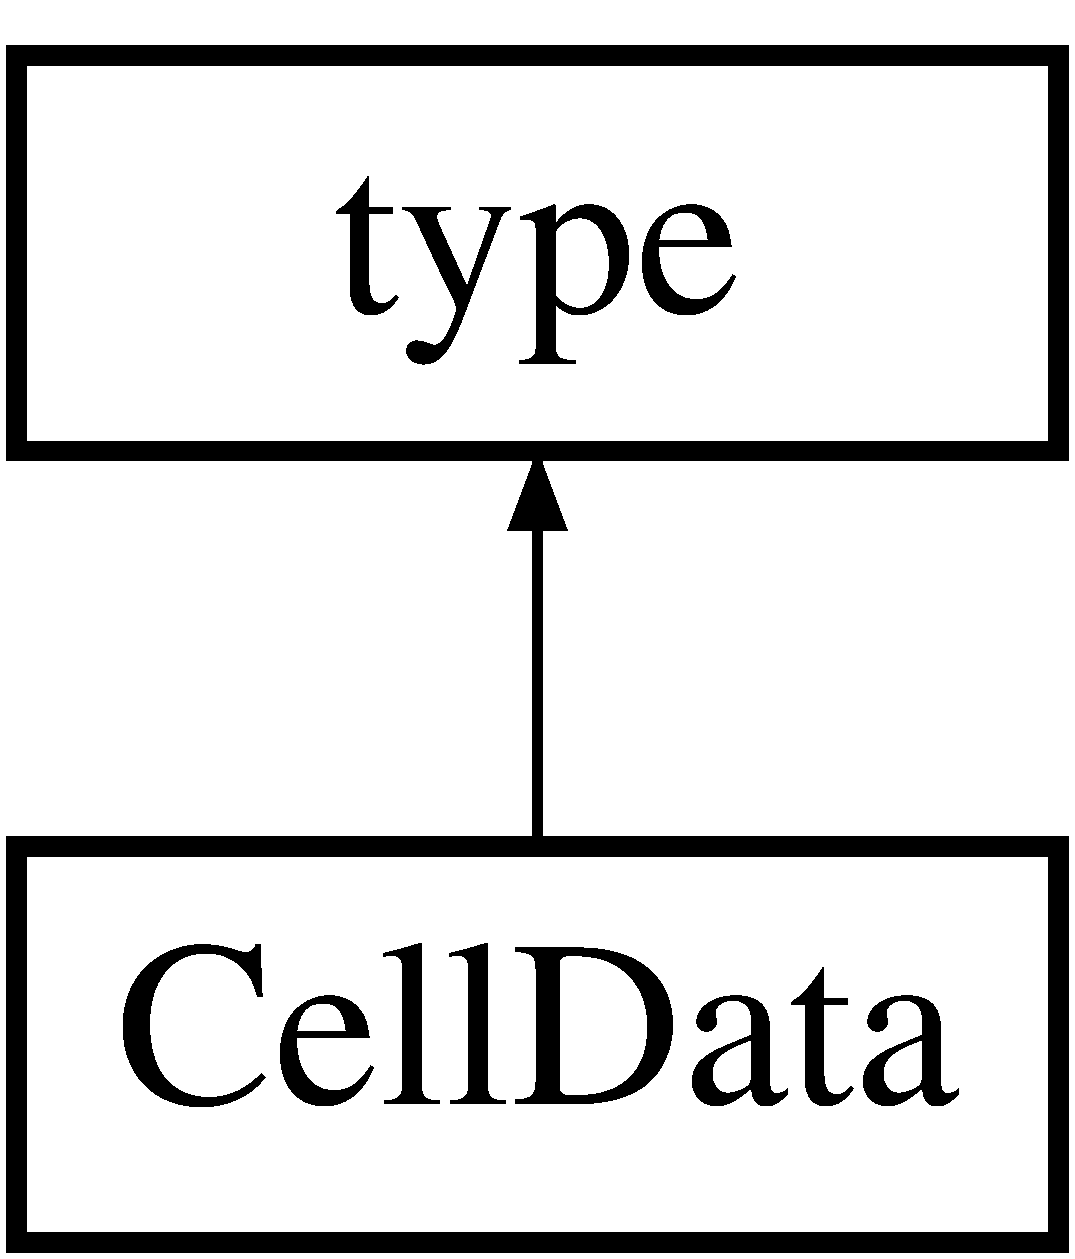
\includegraphics[height=2.000000cm]{classCellData}
\end{center}
\end{figure}
\subsection*{Public Member Functions}
\begin{DoxyCompactItemize}
\item 
virtual \hyperlink{classCellData_aaf439852120aadb5a267799e2a7bf2a3}{$\sim$\-Cell\-Data} ()
\begin{DoxyCompactList}\small\item\em Destructor. \end{DoxyCompactList}\end{DoxyCompactItemize}
\subsection*{Data\-Array}
\label{_amgrp14411195be4ee927801b68cb96397add}%
Accessor and modifier functions for the Data\-Array sequence element. \begin{DoxyCompactItemize}
\item 
typedef \-::\hyperlink{classDataArray__t}{Data\-Array\-\_\-t} \hyperlink{classCellData_a3b277b87cd25225dc944f250bd52057d}{Data\-Array\-\_\-type}
\begin{DoxyCompactList}\small\item\em Element type. \end{DoxyCompactList}\item 
typedef \\*
\-::xsd\-::cxx\-::tree\-::sequence\\*
$<$ \hyperlink{classCellData_a3b277b87cd25225dc944f250bd52057d}{Data\-Array\-\_\-type} $>$ \hyperlink{classCellData_a52b0c8e18ccdb06ed9e6ae76cd809c4a}{Data\-Array\-\_\-sequence}
\begin{DoxyCompactList}\small\item\em Element sequence container type. \end{DoxyCompactList}\item 
typedef \\*
Data\-Array\-\_\-sequence\-::iterator \hyperlink{classCellData_abe0f5b0713690cc81703132bcdccd51f}{Data\-Array\-\_\-iterator}
\begin{DoxyCompactList}\small\item\em Element iterator type. \end{DoxyCompactList}\item 
typedef \\*
Data\-Array\-\_\-sequence\-::const\-\_\-iterator \hyperlink{classCellData_a8213ea10f002fac23b5555ca0b2b2a21}{Data\-Array\-\_\-const\-\_\-iterator}
\begin{DoxyCompactList}\small\item\em Element constant iterator type. \end{DoxyCompactList}\item 
typedef \\*
\-::xsd\-::cxx\-::tree\-::traits\\*
$<$ \hyperlink{classCellData_a3b277b87cd25225dc944f250bd52057d}{Data\-Array\-\_\-type}, char $>$ \hyperlink{classCellData_a03e76eec5af05a6ac5512e9cb80300bd}{Data\-Array\-\_\-traits}
\begin{DoxyCompactList}\small\item\em Element traits type. \end{DoxyCompactList}\item 
const \hyperlink{classCellData_a52b0c8e18ccdb06ed9e6ae76cd809c4a}{Data\-Array\-\_\-sequence} \& \hyperlink{classCellData_af12d2f299905eca541a999dafba1e7e3}{Data\-Array} () const 
\begin{DoxyCompactList}\small\item\em Return a read-\/only (constant) reference to the element sequence. \end{DoxyCompactList}\item 
\hyperlink{classCellData_a52b0c8e18ccdb06ed9e6ae76cd809c4a}{Data\-Array\-\_\-sequence} \& \hyperlink{classCellData_ac40c7e291f83e3e9fabfddeef14131f5}{Data\-Array} ()
\begin{DoxyCompactList}\small\item\em Return a read-\/write reference to the element sequence. \end{DoxyCompactList}\item 
void \hyperlink{classCellData_a9ee9fc1ef295b3ad2c4dc3e9e70ac357}{Data\-Array} (const \hyperlink{classCellData_a52b0c8e18ccdb06ed9e6ae76cd809c4a}{Data\-Array\-\_\-sequence} \&s)
\begin{DoxyCompactList}\small\item\em Copy elements from a given sequence. \end{DoxyCompactList}\end{DoxyCompactItemize}
\subsection*{Constructors}
\begin{DoxyCompactItemize}
\item 
\hyperlink{classCellData_a0d89ba23195659a1fcdc714fa27697a5}{Cell\-Data} ()
\begin{DoxyCompactList}\small\item\em Create an instance from the ultimate base and initializers for required elements and attributes. \end{DoxyCompactList}\item 
\hyperlink{classCellData_ac98b30101e2448016bfa96b9fa6ee18a}{Cell\-Data} (const \-::xercesc\-::\-D\-O\-M\-Element \&e,\-::\hyperlink{namespacexml__schema_a0612287d030cb2732d31a45b258fdc87}{xml\-\_\-schema\-::flags} f=0,\-::\hyperlink{namespacexml__schema_ada9aa30dc722e93ee2ed7243085402a5}{xml\-\_\-schema\-::container} $\ast$c=0)
\begin{DoxyCompactList}\small\item\em Create an instance from a D\-O\-M element. \end{DoxyCompactList}\item 
\hyperlink{classCellData_ae93656ff9893f518c8f1cfdc611c8045}{Cell\-Data} (const \hyperlink{classCellData}{Cell\-Data} \&x,\-::\hyperlink{namespacexml__schema_a0612287d030cb2732d31a45b258fdc87}{xml\-\_\-schema\-::flags} f=0,\-::\hyperlink{namespacexml__schema_ada9aa30dc722e93ee2ed7243085402a5}{xml\-\_\-schema\-::container} $\ast$c=0)
\begin{DoxyCompactList}\small\item\em Copy constructor. \end{DoxyCompactList}\item 
virtual \hyperlink{classCellData}{Cell\-Data} $\ast$ \hyperlink{classCellData_aa17c3a153b3a7692dca562878f3fe3ad}{\-\_\-clone} (\-::\hyperlink{namespacexml__schema_a0612287d030cb2732d31a45b258fdc87}{xml\-\_\-schema\-::flags} f=0,\-::\hyperlink{namespacexml__schema_ada9aa30dc722e93ee2ed7243085402a5}{xml\-\_\-schema\-::container} $\ast$c=0) const 
\begin{DoxyCompactList}\small\item\em Copy the instance polymorphically. \end{DoxyCompactList}\end{DoxyCompactItemize}


\subsection{Detailed Description}
Class corresponding to the Cell\-Data schema type. 

\subsection{Member Typedef Documentation}
\hypertarget{classCellData_a8213ea10f002fac23b5555ca0b2b2a21}{\index{Cell\-Data@{Cell\-Data}!Data\-Array\-\_\-const\-\_\-iterator@{Data\-Array\-\_\-const\-\_\-iterator}}
\index{Data\-Array\-\_\-const\-\_\-iterator@{Data\-Array\-\_\-const\-\_\-iterator}!CellData@{Cell\-Data}}
\subsubsection[{Data\-Array\-\_\-const\-\_\-iterator}]{\setlength{\rightskip}{0pt plus 5cm}typedef Data\-Array\-\_\-sequence\-::const\-\_\-iterator {\bf Cell\-Data\-::\-Data\-Array\-\_\-const\-\_\-iterator}}}\label{classCellData_a8213ea10f002fac23b5555ca0b2b2a21}


Element constant iterator type. 

\hypertarget{classCellData_abe0f5b0713690cc81703132bcdccd51f}{\index{Cell\-Data@{Cell\-Data}!Data\-Array\-\_\-iterator@{Data\-Array\-\_\-iterator}}
\index{Data\-Array\-\_\-iterator@{Data\-Array\-\_\-iterator}!CellData@{Cell\-Data}}
\subsubsection[{Data\-Array\-\_\-iterator}]{\setlength{\rightskip}{0pt plus 5cm}typedef Data\-Array\-\_\-sequence\-::iterator {\bf Cell\-Data\-::\-Data\-Array\-\_\-iterator}}}\label{classCellData_abe0f5b0713690cc81703132bcdccd51f}


Element iterator type. 

\hypertarget{classCellData_a52b0c8e18ccdb06ed9e6ae76cd809c4a}{\index{Cell\-Data@{Cell\-Data}!Data\-Array\-\_\-sequence@{Data\-Array\-\_\-sequence}}
\index{Data\-Array\-\_\-sequence@{Data\-Array\-\_\-sequence}!CellData@{Cell\-Data}}
\subsubsection[{Data\-Array\-\_\-sequence}]{\setlength{\rightskip}{0pt plus 5cm}typedef \-::xsd\-::cxx\-::tree\-::sequence$<$ {\bf Data\-Array\-\_\-type} $>$ {\bf Cell\-Data\-::\-Data\-Array\-\_\-sequence}}}\label{classCellData_a52b0c8e18ccdb06ed9e6ae76cd809c4a}


Element sequence container type. 

\hypertarget{classCellData_a03e76eec5af05a6ac5512e9cb80300bd}{\index{Cell\-Data@{Cell\-Data}!Data\-Array\-\_\-traits@{Data\-Array\-\_\-traits}}
\index{Data\-Array\-\_\-traits@{Data\-Array\-\_\-traits}!CellData@{Cell\-Data}}
\subsubsection[{Data\-Array\-\_\-traits}]{\setlength{\rightskip}{0pt plus 5cm}typedef \-::xsd\-::cxx\-::tree\-::traits$<$ {\bf Data\-Array\-\_\-type}, char $>$ {\bf Cell\-Data\-::\-Data\-Array\-\_\-traits}}}\label{classCellData_a03e76eec5af05a6ac5512e9cb80300bd}


Element traits type. 

\hypertarget{classCellData_a3b277b87cd25225dc944f250bd52057d}{\index{Cell\-Data@{Cell\-Data}!Data\-Array\-\_\-type@{Data\-Array\-\_\-type}}
\index{Data\-Array\-\_\-type@{Data\-Array\-\_\-type}!CellData@{Cell\-Data}}
\subsubsection[{Data\-Array\-\_\-type}]{\setlength{\rightskip}{0pt plus 5cm}typedef \-::{\bf Data\-Array\-\_\-t} {\bf Cell\-Data\-::\-Data\-Array\-\_\-type}}}\label{classCellData_a3b277b87cd25225dc944f250bd52057d}


Element type. 



\subsection{Constructor \& Destructor Documentation}
\hypertarget{classCellData_a0d89ba23195659a1fcdc714fa27697a5}{\index{Cell\-Data@{Cell\-Data}!Cell\-Data@{Cell\-Data}}
\index{Cell\-Data@{Cell\-Data}!CellData@{Cell\-Data}}
\subsubsection[{Cell\-Data}]{\setlength{\rightskip}{0pt plus 5cm}Cell\-Data\-::\-Cell\-Data (
\begin{DoxyParamCaption}
{}
\end{DoxyParamCaption}
)}}\label{classCellData_a0d89ba23195659a1fcdc714fa27697a5}


Create an instance from the ultimate base and initializers for required elements and attributes. 

\hypertarget{classCellData_ac98b30101e2448016bfa96b9fa6ee18a}{\index{Cell\-Data@{Cell\-Data}!Cell\-Data@{Cell\-Data}}
\index{Cell\-Data@{Cell\-Data}!CellData@{Cell\-Data}}
\subsubsection[{Cell\-Data}]{\setlength{\rightskip}{0pt plus 5cm}Cell\-Data\-::\-Cell\-Data (
\begin{DoxyParamCaption}
\item[{const \-::xercesc\-::\-D\-O\-M\-Element \&}]{e, }
\item[{\-::{\bf xml\-\_\-schema\-::flags}}]{f = {\ttfamily 0}, }
\item[{\-::{\bf xml\-\_\-schema\-::container} $\ast$}]{c = {\ttfamily 0}}
\end{DoxyParamCaption}
)}}\label{classCellData_ac98b30101e2448016bfa96b9fa6ee18a}


Create an instance from a D\-O\-M element. 


\begin{DoxyParams}{Parameters}
{\em e} & A D\-O\-M element to extract the data from. \\
\hline
{\em f} & Flags to create the new instance with. \\
\hline
{\em c} & A pointer to the object that will contain the new instance. \\
\hline
\end{DoxyParams}
\hypertarget{classCellData_ae93656ff9893f518c8f1cfdc611c8045}{\index{Cell\-Data@{Cell\-Data}!Cell\-Data@{Cell\-Data}}
\index{Cell\-Data@{Cell\-Data}!CellData@{Cell\-Data}}
\subsubsection[{Cell\-Data}]{\setlength{\rightskip}{0pt plus 5cm}Cell\-Data\-::\-Cell\-Data (
\begin{DoxyParamCaption}
\item[{const {\bf Cell\-Data} \&}]{x, }
\item[{\-::{\bf xml\-\_\-schema\-::flags}}]{f = {\ttfamily 0}, }
\item[{\-::{\bf xml\-\_\-schema\-::container} $\ast$}]{c = {\ttfamily 0}}
\end{DoxyParamCaption}
)}}\label{classCellData_ae93656ff9893f518c8f1cfdc611c8045}


Copy constructor. 


\begin{DoxyParams}{Parameters}
{\em x} & An instance to make a copy of. \\
\hline
{\em f} & Flags to create the copy with. \\
\hline
{\em c} & A pointer to the object that will contain the copy.\\
\hline
\end{DoxyParams}
For polymorphic object models use the {\ttfamily \-\_\-clone} function instead. \hypertarget{classCellData_aaf439852120aadb5a267799e2a7bf2a3}{\index{Cell\-Data@{Cell\-Data}!$\sim$\-Cell\-Data@{$\sim$\-Cell\-Data}}
\index{$\sim$\-Cell\-Data@{$\sim$\-Cell\-Data}!CellData@{Cell\-Data}}
\subsubsection[{$\sim$\-Cell\-Data}]{\setlength{\rightskip}{0pt plus 5cm}Cell\-Data\-::$\sim$\-Cell\-Data (
\begin{DoxyParamCaption}
{}
\end{DoxyParamCaption}
)\hspace{0.3cm}{\ttfamily [virtual]}}}\label{classCellData_aaf439852120aadb5a267799e2a7bf2a3}


Destructor. 



\subsection{Member Function Documentation}
\hypertarget{classCellData_aa17c3a153b3a7692dca562878f3fe3ad}{\index{Cell\-Data@{Cell\-Data}!\-\_\-clone@{\-\_\-clone}}
\index{\-\_\-clone@{\-\_\-clone}!CellData@{Cell\-Data}}
\subsubsection[{\-\_\-clone}]{\setlength{\rightskip}{0pt plus 5cm}{\bf Cell\-Data} $\ast$ Cell\-Data\-::\-\_\-clone (
\begin{DoxyParamCaption}
\item[{\-::{\bf xml\-\_\-schema\-::flags}}]{f = {\ttfamily 0}, }
\item[{\-::{\bf xml\-\_\-schema\-::container} $\ast$}]{c = {\ttfamily 0}}
\end{DoxyParamCaption}
) const\hspace{0.3cm}{\ttfamily [virtual]}}}\label{classCellData_aa17c3a153b3a7692dca562878f3fe3ad}


Copy the instance polymorphically. 


\begin{DoxyParams}{Parameters}
{\em f} & Flags to create the copy with. \\
\hline
{\em c} & A pointer to the object that will contain the copy. \\
\hline
\end{DoxyParams}
\begin{DoxyReturn}{Returns}
A pointer to the dynamically allocated copy.
\end{DoxyReturn}
This function ensures that the dynamic type of the instance is used for copying and should be used for polymorphic object models instead of the copy constructor. \hypertarget{classCellData_af12d2f299905eca541a999dafba1e7e3}{\index{Cell\-Data@{Cell\-Data}!Data\-Array@{Data\-Array}}
\index{Data\-Array@{Data\-Array}!CellData@{Cell\-Data}}
\subsubsection[{Data\-Array}]{\setlength{\rightskip}{0pt plus 5cm}const {\bf Cell\-Data\-::\-Data\-Array\-\_\-sequence} \& Cell\-Data\-::\-Data\-Array (
\begin{DoxyParamCaption}
{}
\end{DoxyParamCaption}
) const}}\label{classCellData_af12d2f299905eca541a999dafba1e7e3}


Return a read-\/only (constant) reference to the element sequence. 

\begin{DoxyReturn}{Returns}
A constant reference to the sequence container. 
\end{DoxyReturn}
\hypertarget{classCellData_ac40c7e291f83e3e9fabfddeef14131f5}{\index{Cell\-Data@{Cell\-Data}!Data\-Array@{Data\-Array}}
\index{Data\-Array@{Data\-Array}!CellData@{Cell\-Data}}
\subsubsection[{Data\-Array}]{\setlength{\rightskip}{0pt plus 5cm}{\bf Cell\-Data\-::\-Data\-Array\-\_\-sequence} \& Cell\-Data\-::\-Data\-Array (
\begin{DoxyParamCaption}
{}
\end{DoxyParamCaption}
)}}\label{classCellData_ac40c7e291f83e3e9fabfddeef14131f5}


Return a read-\/write reference to the element sequence. 

\begin{DoxyReturn}{Returns}
A reference to the sequence container. 
\end{DoxyReturn}
\hypertarget{classCellData_a9ee9fc1ef295b3ad2c4dc3e9e70ac357}{\index{Cell\-Data@{Cell\-Data}!Data\-Array@{Data\-Array}}
\index{Data\-Array@{Data\-Array}!CellData@{Cell\-Data}}
\subsubsection[{Data\-Array}]{\setlength{\rightskip}{0pt plus 5cm}void Cell\-Data\-::\-Data\-Array (
\begin{DoxyParamCaption}
\item[{const {\bf Data\-Array\-\_\-sequence} \&}]{s}
\end{DoxyParamCaption}
)}}\label{classCellData_a9ee9fc1ef295b3ad2c4dc3e9e70ac357}


Copy elements from a given sequence. 


\begin{DoxyParams}{Parameters}
{\em s} & A sequence to copy elements from.\\
\hline
\end{DoxyParams}
For each element in {\itshape s} this function makes a copy and adds it to the sequence. Note that this operation completely changes the sequence and all old elements will be lost. 

The documentation for this class was generated from the following files\-:\begin{DoxyCompactItemize}
\item 
src/output\-Writer/\hyperlink{vtk-unstructured_8h}{vtk-\/unstructured.\-h}\item 
src/output\-Writer/\hyperlink{vtk-unstructured_8cpp}{vtk-\/unstructured.\-cpp}\end{DoxyCompactItemize}

\hypertarget{classCells}{\section{Cells Class Reference}
\label{classCells}\index{Cells@{Cells}}
}


Class corresponding to the Cells schema type.  




{\ttfamily \#include $<$vtk-\/unstructured.\-h$>$}

Inheritance diagram for Cells\-:\begin{figure}[H]
\begin{center}
\leavevmode
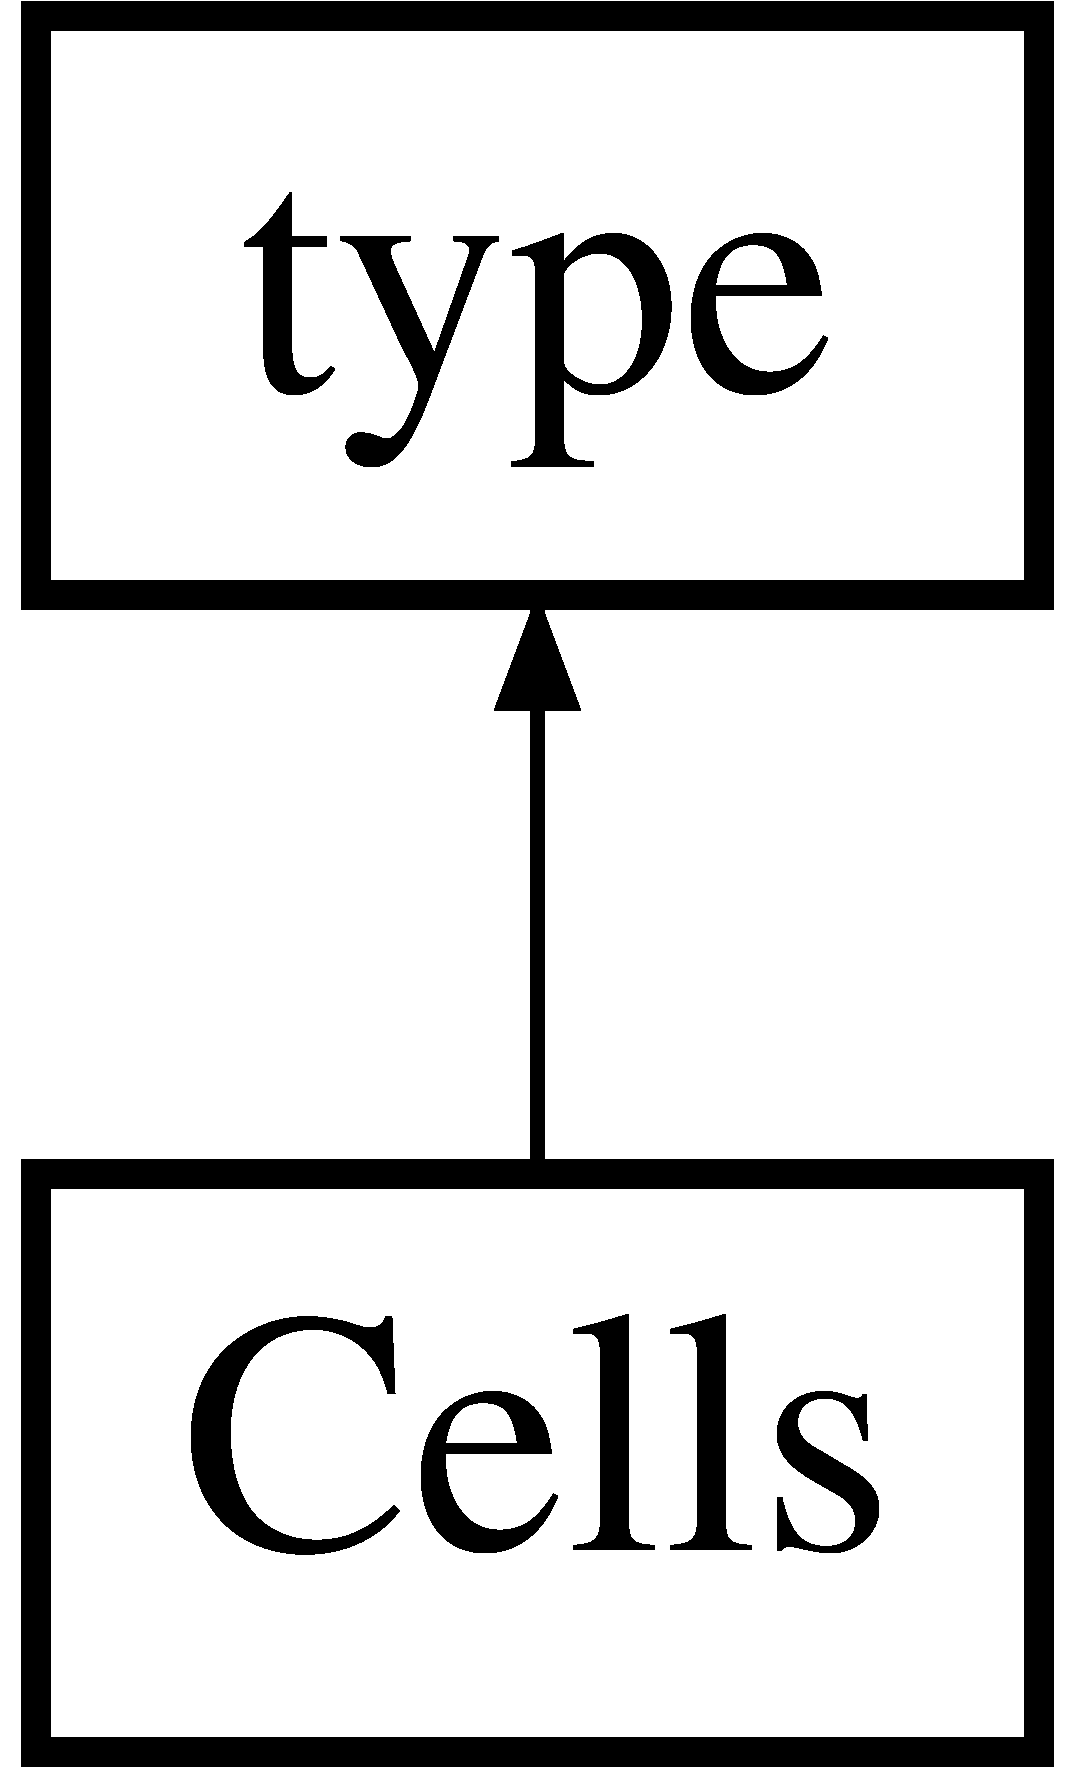
\includegraphics[height=2.000000cm]{classCells}
\end{center}
\end{figure}
\subsection*{Public Member Functions}
\begin{DoxyCompactItemize}
\item 
virtual \hyperlink{classCells_aab121634db81b439226a33fd099fb3c1}{$\sim$\-Cells} ()
\begin{DoxyCompactList}\small\item\em Destructor. \end{DoxyCompactList}\end{DoxyCompactItemize}
\subsection*{Data\-Array}
\label{_amgrp14411195be4ee927801b68cb96397add}%
Accessor and modifier functions for the Data\-Array sequence element. \begin{DoxyCompactItemize}
\item 
typedef \-::\hyperlink{classDataArray__t}{Data\-Array\-\_\-t} \hyperlink{classCells_ad69e76337c22596e70b27d93c54dd722}{Data\-Array\-\_\-type}
\begin{DoxyCompactList}\small\item\em Element type. \end{DoxyCompactList}\item 
typedef \\*
\-::xsd\-::cxx\-::tree\-::sequence\\*
$<$ \hyperlink{classCells_ad69e76337c22596e70b27d93c54dd722}{Data\-Array\-\_\-type} $>$ \hyperlink{classCells_ae2856ec1cc2c6d6a2ccac9de9a22c7b7}{Data\-Array\-\_\-sequence}
\begin{DoxyCompactList}\small\item\em Element sequence container type. \end{DoxyCompactList}\item 
typedef \\*
Data\-Array\-\_\-sequence\-::iterator \hyperlink{classCells_a1873efdee2bb668676d01a7a5010faa2}{Data\-Array\-\_\-iterator}
\begin{DoxyCompactList}\small\item\em Element iterator type. \end{DoxyCompactList}\item 
typedef \\*
Data\-Array\-\_\-sequence\-::const\-\_\-iterator \hyperlink{classCells_ad01c81703074599471cd6159cdea1ac1}{Data\-Array\-\_\-const\-\_\-iterator}
\begin{DoxyCompactList}\small\item\em Element constant iterator type. \end{DoxyCompactList}\item 
typedef \\*
\-::xsd\-::cxx\-::tree\-::traits\\*
$<$ \hyperlink{classCells_ad69e76337c22596e70b27d93c54dd722}{Data\-Array\-\_\-type}, char $>$ \hyperlink{classCells_ac35ecebe10914f3d35e85589e998462b}{Data\-Array\-\_\-traits}
\begin{DoxyCompactList}\small\item\em Element traits type. \end{DoxyCompactList}\item 
const \hyperlink{classCells_ae2856ec1cc2c6d6a2ccac9de9a22c7b7}{Data\-Array\-\_\-sequence} \& \hyperlink{classCells_a8844f4f5a352181f29e8589d72fba69f}{Data\-Array} () const 
\begin{DoxyCompactList}\small\item\em Return a read-\/only (constant) reference to the element sequence. \end{DoxyCompactList}\item 
\hyperlink{classCells_ae2856ec1cc2c6d6a2ccac9de9a22c7b7}{Data\-Array\-\_\-sequence} \& \hyperlink{classCells_a6114566d42273127f9cb92b1d0f09cb5}{Data\-Array} ()
\begin{DoxyCompactList}\small\item\em Return a read-\/write reference to the element sequence. \end{DoxyCompactList}\item 
void \hyperlink{classCells_a52c9971e15358118dd90ecf68b26601e}{Data\-Array} (const \hyperlink{classCells_ae2856ec1cc2c6d6a2ccac9de9a22c7b7}{Data\-Array\-\_\-sequence} \&s)
\begin{DoxyCompactList}\small\item\em Copy elements from a given sequence. \end{DoxyCompactList}\end{DoxyCompactItemize}
\subsection*{Constructors}
\begin{DoxyCompactItemize}
\item 
\hyperlink{classCells_a092d62bc15648a54755a413dbf9a2db0}{Cells} ()
\begin{DoxyCompactList}\small\item\em Create an instance from the ultimate base and initializers for required elements and attributes. \end{DoxyCompactList}\item 
\hyperlink{classCells_a79e3031094d928c8d275198201d44f0c}{Cells} (const \-::xercesc\-::\-D\-O\-M\-Element \&e,\-::\hyperlink{namespacexml__schema_a0612287d030cb2732d31a45b258fdc87}{xml\-\_\-schema\-::flags} f=0,\-::\hyperlink{namespacexml__schema_ada9aa30dc722e93ee2ed7243085402a5}{xml\-\_\-schema\-::container} $\ast$c=0)
\begin{DoxyCompactList}\small\item\em Create an instance from a D\-O\-M element. \end{DoxyCompactList}\item 
\hyperlink{classCells_a9322653263fb302eb7068be10b1b364f}{Cells} (const \hyperlink{classCells}{Cells} \&x,\-::\hyperlink{namespacexml__schema_a0612287d030cb2732d31a45b258fdc87}{xml\-\_\-schema\-::flags} f=0,\-::\hyperlink{namespacexml__schema_ada9aa30dc722e93ee2ed7243085402a5}{xml\-\_\-schema\-::container} $\ast$c=0)
\begin{DoxyCompactList}\small\item\em Copy constructor. \end{DoxyCompactList}\item 
virtual \hyperlink{classCells}{Cells} $\ast$ \hyperlink{classCells_a67e7fa1cc404dcc4814011ca179f8a83}{\-\_\-clone} (\-::\hyperlink{namespacexml__schema_a0612287d030cb2732d31a45b258fdc87}{xml\-\_\-schema\-::flags} f=0,\-::\hyperlink{namespacexml__schema_ada9aa30dc722e93ee2ed7243085402a5}{xml\-\_\-schema\-::container} $\ast$c=0) const 
\begin{DoxyCompactList}\small\item\em Copy the instance polymorphically. \end{DoxyCompactList}\end{DoxyCompactItemize}


\subsection{Detailed Description}
Class corresponding to the Cells schema type. 

\subsection{Member Typedef Documentation}
\hypertarget{classCells_ad01c81703074599471cd6159cdea1ac1}{\index{Cells@{Cells}!Data\-Array\-\_\-const\-\_\-iterator@{Data\-Array\-\_\-const\-\_\-iterator}}
\index{Data\-Array\-\_\-const\-\_\-iterator@{Data\-Array\-\_\-const\-\_\-iterator}!Cells@{Cells}}
\subsubsection[{Data\-Array\-\_\-const\-\_\-iterator}]{\setlength{\rightskip}{0pt plus 5cm}typedef Data\-Array\-\_\-sequence\-::const\-\_\-iterator {\bf Cells\-::\-Data\-Array\-\_\-const\-\_\-iterator}}}\label{classCells_ad01c81703074599471cd6159cdea1ac1}


Element constant iterator type. 

\hypertarget{classCells_a1873efdee2bb668676d01a7a5010faa2}{\index{Cells@{Cells}!Data\-Array\-\_\-iterator@{Data\-Array\-\_\-iterator}}
\index{Data\-Array\-\_\-iterator@{Data\-Array\-\_\-iterator}!Cells@{Cells}}
\subsubsection[{Data\-Array\-\_\-iterator}]{\setlength{\rightskip}{0pt plus 5cm}typedef Data\-Array\-\_\-sequence\-::iterator {\bf Cells\-::\-Data\-Array\-\_\-iterator}}}\label{classCells_a1873efdee2bb668676d01a7a5010faa2}


Element iterator type. 

\hypertarget{classCells_ae2856ec1cc2c6d6a2ccac9de9a22c7b7}{\index{Cells@{Cells}!Data\-Array\-\_\-sequence@{Data\-Array\-\_\-sequence}}
\index{Data\-Array\-\_\-sequence@{Data\-Array\-\_\-sequence}!Cells@{Cells}}
\subsubsection[{Data\-Array\-\_\-sequence}]{\setlength{\rightskip}{0pt plus 5cm}typedef \-::xsd\-::cxx\-::tree\-::sequence$<$ {\bf Data\-Array\-\_\-type} $>$ {\bf Cells\-::\-Data\-Array\-\_\-sequence}}}\label{classCells_ae2856ec1cc2c6d6a2ccac9de9a22c7b7}


Element sequence container type. 

\hypertarget{classCells_ac35ecebe10914f3d35e85589e998462b}{\index{Cells@{Cells}!Data\-Array\-\_\-traits@{Data\-Array\-\_\-traits}}
\index{Data\-Array\-\_\-traits@{Data\-Array\-\_\-traits}!Cells@{Cells}}
\subsubsection[{Data\-Array\-\_\-traits}]{\setlength{\rightskip}{0pt plus 5cm}typedef \-::xsd\-::cxx\-::tree\-::traits$<$ {\bf Data\-Array\-\_\-type}, char $>$ {\bf Cells\-::\-Data\-Array\-\_\-traits}}}\label{classCells_ac35ecebe10914f3d35e85589e998462b}


Element traits type. 

\hypertarget{classCells_ad69e76337c22596e70b27d93c54dd722}{\index{Cells@{Cells}!Data\-Array\-\_\-type@{Data\-Array\-\_\-type}}
\index{Data\-Array\-\_\-type@{Data\-Array\-\_\-type}!Cells@{Cells}}
\subsubsection[{Data\-Array\-\_\-type}]{\setlength{\rightskip}{0pt plus 5cm}typedef \-::{\bf Data\-Array\-\_\-t} {\bf Cells\-::\-Data\-Array\-\_\-type}}}\label{classCells_ad69e76337c22596e70b27d93c54dd722}


Element type. 



\subsection{Constructor \& Destructor Documentation}
\hypertarget{classCells_a092d62bc15648a54755a413dbf9a2db0}{\index{Cells@{Cells}!Cells@{Cells}}
\index{Cells@{Cells}!Cells@{Cells}}
\subsubsection[{Cells}]{\setlength{\rightskip}{0pt plus 5cm}Cells\-::\-Cells (
\begin{DoxyParamCaption}
{}
\end{DoxyParamCaption}
)}}\label{classCells_a092d62bc15648a54755a413dbf9a2db0}


Create an instance from the ultimate base and initializers for required elements and attributes. 

\hypertarget{classCells_a79e3031094d928c8d275198201d44f0c}{\index{Cells@{Cells}!Cells@{Cells}}
\index{Cells@{Cells}!Cells@{Cells}}
\subsubsection[{Cells}]{\setlength{\rightskip}{0pt plus 5cm}Cells\-::\-Cells (
\begin{DoxyParamCaption}
\item[{const \-::xercesc\-::\-D\-O\-M\-Element \&}]{e, }
\item[{\-::{\bf xml\-\_\-schema\-::flags}}]{f = {\ttfamily 0}, }
\item[{\-::{\bf xml\-\_\-schema\-::container} $\ast$}]{c = {\ttfamily 0}}
\end{DoxyParamCaption}
)}}\label{classCells_a79e3031094d928c8d275198201d44f0c}


Create an instance from a D\-O\-M element. 


\begin{DoxyParams}{Parameters}
{\em e} & A D\-O\-M element to extract the data from. \\
\hline
{\em f} & Flags to create the new instance with. \\
\hline
{\em c} & A pointer to the object that will contain the new instance. \\
\hline
\end{DoxyParams}
\hypertarget{classCells_a9322653263fb302eb7068be10b1b364f}{\index{Cells@{Cells}!Cells@{Cells}}
\index{Cells@{Cells}!Cells@{Cells}}
\subsubsection[{Cells}]{\setlength{\rightskip}{0pt plus 5cm}Cells\-::\-Cells (
\begin{DoxyParamCaption}
\item[{const {\bf Cells} \&}]{x, }
\item[{\-::{\bf xml\-\_\-schema\-::flags}}]{f = {\ttfamily 0}, }
\item[{\-::{\bf xml\-\_\-schema\-::container} $\ast$}]{c = {\ttfamily 0}}
\end{DoxyParamCaption}
)}}\label{classCells_a9322653263fb302eb7068be10b1b364f}


Copy constructor. 


\begin{DoxyParams}{Parameters}
{\em x} & An instance to make a copy of. \\
\hline
{\em f} & Flags to create the copy with. \\
\hline
{\em c} & A pointer to the object that will contain the copy.\\
\hline
\end{DoxyParams}
For polymorphic object models use the {\ttfamily \-\_\-clone} function instead. \hypertarget{classCells_aab121634db81b439226a33fd099fb3c1}{\index{Cells@{Cells}!$\sim$\-Cells@{$\sim$\-Cells}}
\index{$\sim$\-Cells@{$\sim$\-Cells}!Cells@{Cells}}
\subsubsection[{$\sim$\-Cells}]{\setlength{\rightskip}{0pt plus 5cm}Cells\-::$\sim$\-Cells (
\begin{DoxyParamCaption}
{}
\end{DoxyParamCaption}
)\hspace{0.3cm}{\ttfamily [virtual]}}}\label{classCells_aab121634db81b439226a33fd099fb3c1}


Destructor. 



\subsection{Member Function Documentation}
\hypertarget{classCells_a67e7fa1cc404dcc4814011ca179f8a83}{\index{Cells@{Cells}!\-\_\-clone@{\-\_\-clone}}
\index{\-\_\-clone@{\-\_\-clone}!Cells@{Cells}}
\subsubsection[{\-\_\-clone}]{\setlength{\rightskip}{0pt plus 5cm}{\bf Cells} $\ast$ Cells\-::\-\_\-clone (
\begin{DoxyParamCaption}
\item[{\-::{\bf xml\-\_\-schema\-::flags}}]{f = {\ttfamily 0}, }
\item[{\-::{\bf xml\-\_\-schema\-::container} $\ast$}]{c = {\ttfamily 0}}
\end{DoxyParamCaption}
) const\hspace{0.3cm}{\ttfamily [virtual]}}}\label{classCells_a67e7fa1cc404dcc4814011ca179f8a83}


Copy the instance polymorphically. 


\begin{DoxyParams}{Parameters}
{\em f} & Flags to create the copy with. \\
\hline
{\em c} & A pointer to the object that will contain the copy. \\
\hline
\end{DoxyParams}
\begin{DoxyReturn}{Returns}
A pointer to the dynamically allocated copy.
\end{DoxyReturn}
This function ensures that the dynamic type of the instance is used for copying and should be used for polymorphic object models instead of the copy constructor. \hypertarget{classCells_a8844f4f5a352181f29e8589d72fba69f}{\index{Cells@{Cells}!Data\-Array@{Data\-Array}}
\index{Data\-Array@{Data\-Array}!Cells@{Cells}}
\subsubsection[{Data\-Array}]{\setlength{\rightskip}{0pt plus 5cm}const {\bf Cells\-::\-Data\-Array\-\_\-sequence} \& Cells\-::\-Data\-Array (
\begin{DoxyParamCaption}
{}
\end{DoxyParamCaption}
) const}}\label{classCells_a8844f4f5a352181f29e8589d72fba69f}


Return a read-\/only (constant) reference to the element sequence. 

\begin{DoxyReturn}{Returns}
A constant reference to the sequence container. 
\end{DoxyReturn}
\hypertarget{classCells_a6114566d42273127f9cb92b1d0f09cb5}{\index{Cells@{Cells}!Data\-Array@{Data\-Array}}
\index{Data\-Array@{Data\-Array}!Cells@{Cells}}
\subsubsection[{Data\-Array}]{\setlength{\rightskip}{0pt plus 5cm}{\bf Cells\-::\-Data\-Array\-\_\-sequence} \& Cells\-::\-Data\-Array (
\begin{DoxyParamCaption}
{}
\end{DoxyParamCaption}
)}}\label{classCells_a6114566d42273127f9cb92b1d0f09cb5}


Return a read-\/write reference to the element sequence. 

\begin{DoxyReturn}{Returns}
A reference to the sequence container. 
\end{DoxyReturn}
\hypertarget{classCells_a52c9971e15358118dd90ecf68b26601e}{\index{Cells@{Cells}!Data\-Array@{Data\-Array}}
\index{Data\-Array@{Data\-Array}!Cells@{Cells}}
\subsubsection[{Data\-Array}]{\setlength{\rightskip}{0pt plus 5cm}void Cells\-::\-Data\-Array (
\begin{DoxyParamCaption}
\item[{const {\bf Data\-Array\-\_\-sequence} \&}]{s}
\end{DoxyParamCaption}
)}}\label{classCells_a52c9971e15358118dd90ecf68b26601e}


Copy elements from a given sequence. 


\begin{DoxyParams}{Parameters}
{\em s} & A sequence to copy elements from.\\
\hline
\end{DoxyParams}
For each element in {\itshape s} this function makes a copy and adds it to the sequence. Note that this operation completely changes the sequence and all old elements will be lost. 

The documentation for this class was generated from the following files\-:\begin{DoxyCompactItemize}
\item 
src/output\-Writer/\hyperlink{vtk-unstructured_8h}{vtk-\/unstructured.\-h}\item 
src/output\-Writer/\hyperlink{vtk-unstructured_8cpp}{vtk-\/unstructured.\-cpp}\end{DoxyCompactItemize}

\hypertarget{classcenterPos__t}{\section{center\-Pos\-\_\-t Class Reference}
\label{classcenterPos__t}\index{center\-Pos\-\_\-t@{center\-Pos\-\_\-t}}
}


{\ttfamily \#include $<$Input\-Spheres.\-h$>$}

Inheritance diagram for center\-Pos\-\_\-t\-:\begin{figure}[H]
\begin{center}
\leavevmode
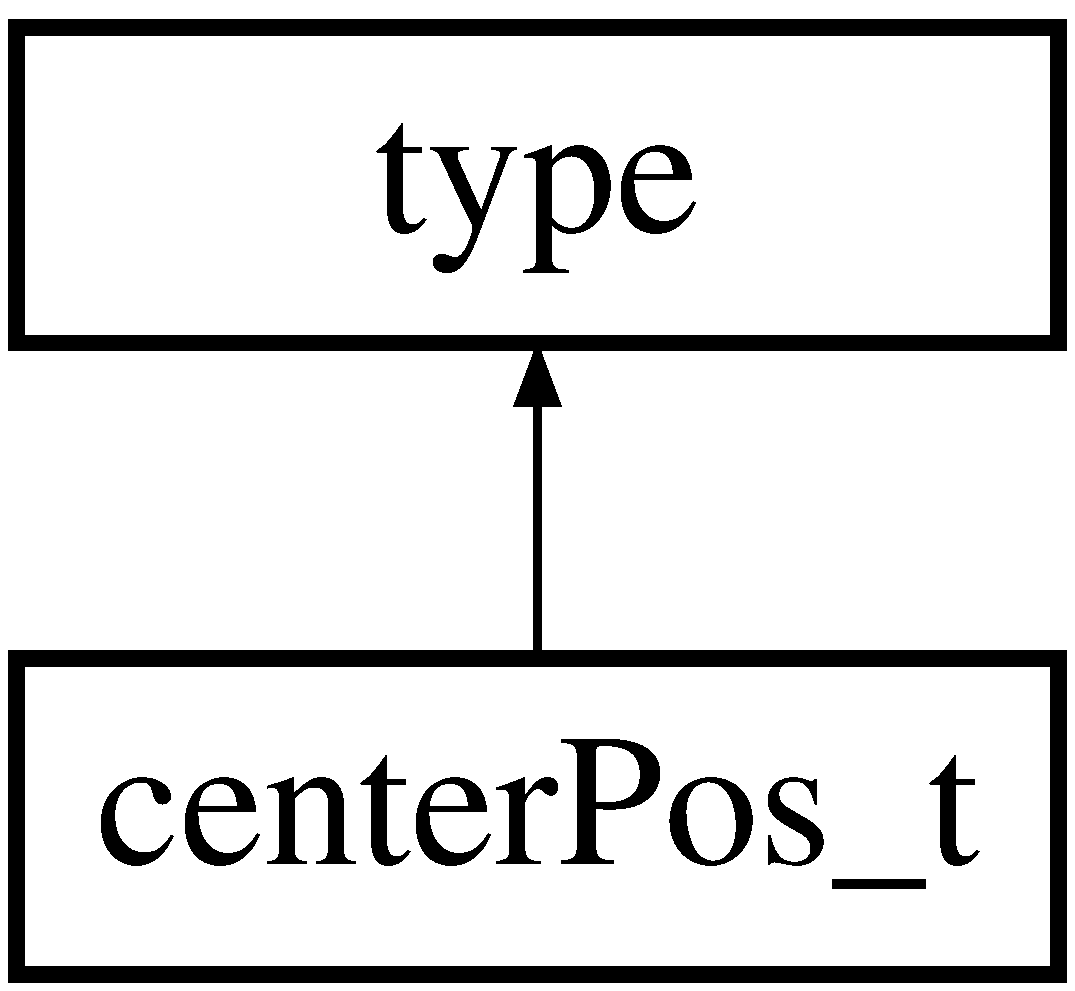
\includegraphics[height=2.000000cm]{classcenterPos__t}
\end{center}
\end{figure}
\subsection*{Public Types}
\begin{DoxyCompactItemize}
\item 
typedef \-::\hyperlink{namespacexml__schema_a69bfaf24f63a8c18ebd8e21db6b343df}{xml\-\_\-schema\-::decimal} \hyperlink{classcenterPos__t_ad9202ab9a64d0ac44ac212e2b8ad52f9}{x\-\_\-type}
\item 
typedef \\*
\-::xsd\-::cxx\-::tree\-::traits\\*
$<$ \hyperlink{classcenterPos__t_ad9202ab9a64d0ac44ac212e2b8ad52f9}{x\-\_\-type}, char,\-::xsd\-::cxx\-::tree\-::schema\-\_\-type\-::decimal $>$ \hyperlink{classcenterPos__t_ab983e22a2d65a5fd634f53910e7ee483}{x\-\_\-traits}
\item 
typedef \-::\hyperlink{namespacexml__schema_a69bfaf24f63a8c18ebd8e21db6b343df}{xml\-\_\-schema\-::decimal} \hyperlink{classcenterPos__t_a729ec04aac9d1066004b319cca2879fd}{y\-\_\-type}
\item 
typedef \\*
\-::xsd\-::cxx\-::tree\-::traits\\*
$<$ \hyperlink{classcenterPos__t_a729ec04aac9d1066004b319cca2879fd}{y\-\_\-type}, char,\-::xsd\-::cxx\-::tree\-::schema\-\_\-type\-::decimal $>$ \hyperlink{classcenterPos__t_a3a852dc42bb49f7aba36332b422e9430}{y\-\_\-traits}
\item 
typedef \-::\hyperlink{namespacexml__schema_a69bfaf24f63a8c18ebd8e21db6b343df}{xml\-\_\-schema\-::decimal} \hyperlink{classcenterPos__t_a6c424433a912263b9c8644a89ad14082}{z\-\_\-type}
\item 
typedef \\*
\-::xsd\-::cxx\-::tree\-::traits\\*
$<$ \hyperlink{classcenterPos__t_a6c424433a912263b9c8644a89ad14082}{z\-\_\-type}, char,\-::xsd\-::cxx\-::tree\-::schema\-\_\-type\-::decimal $>$ \hyperlink{classcenterPos__t_a4dd2aec563bb681d33444f495887ebb8}{z\-\_\-traits}
\end{DoxyCompactItemize}
\subsection*{Public Member Functions}
\begin{DoxyCompactItemize}
\item 
const \hyperlink{classcenterPos__t_ad9202ab9a64d0ac44ac212e2b8ad52f9}{x\-\_\-type} \& \hyperlink{classcenterPos__t_aed87cbea230ad34c4154ce268a729c61}{x} () const 
\item 
\hyperlink{classcenterPos__t_ad9202ab9a64d0ac44ac212e2b8ad52f9}{x\-\_\-type} \& \hyperlink{classcenterPos__t_af0cc4301b30b5e371f9a870332f57cee}{x} ()
\item 
void \hyperlink{classcenterPos__t_a96929b2d9933a718295f505986b7404a}{x} (const \hyperlink{classcenterPos__t_ad9202ab9a64d0ac44ac212e2b8ad52f9}{x\-\_\-type} \&x)
\item 
const \hyperlink{classcenterPos__t_a729ec04aac9d1066004b319cca2879fd}{y\-\_\-type} \& \hyperlink{classcenterPos__t_abdbdcbe58018d0aea3014ccc156beb7f}{y} () const 
\item 
\hyperlink{classcenterPos__t_a729ec04aac9d1066004b319cca2879fd}{y\-\_\-type} \& \hyperlink{classcenterPos__t_a2557e1f42e6e7a3d5e9a61dd549ca1da}{y} ()
\item 
void \hyperlink{classcenterPos__t_ad5fd4ab7ecf57c42dc5e9c1109bd2b42}{y} (const \hyperlink{classcenterPos__t_a729ec04aac9d1066004b319cca2879fd}{y\-\_\-type} \&\hyperlink{classcenterPos__t_aed87cbea230ad34c4154ce268a729c61}{x})
\item 
const \hyperlink{classcenterPos__t_a6c424433a912263b9c8644a89ad14082}{z\-\_\-type} \& \hyperlink{classcenterPos__t_acc523766223f841534ae7c497dac1282}{z} () const 
\item 
\hyperlink{classcenterPos__t_a6c424433a912263b9c8644a89ad14082}{z\-\_\-type} \& \hyperlink{classcenterPos__t_a8d413cf482c77b8798325895af33d2f1}{z} ()
\item 
void \hyperlink{classcenterPos__t_a4efe9adefd41d738075de58f1ad92cb1}{z} (const \hyperlink{classcenterPos__t_a6c424433a912263b9c8644a89ad14082}{z\-\_\-type} \&\hyperlink{classcenterPos__t_aed87cbea230ad34c4154ce268a729c61}{x})
\item 
\hyperlink{classcenterPos__t_a8ada28b759c2bf0cf3194e2fa1bd345e}{center\-Pos\-\_\-t} (const \hyperlink{classcenterPos__t_ad9202ab9a64d0ac44ac212e2b8ad52f9}{x\-\_\-type} \&, const \hyperlink{classcenterPos__t_a729ec04aac9d1066004b319cca2879fd}{y\-\_\-type} \&, const \hyperlink{classcenterPos__t_a6c424433a912263b9c8644a89ad14082}{z\-\_\-type} \&)
\item 
\hyperlink{classcenterPos__t_ac9f4d867513a4ff3f2ed8ca249818410}{center\-Pos\-\_\-t} (const \-::xercesc\-::\-D\-O\-M\-Element \&e,\-::\hyperlink{namespacexml__schema_a0612287d030cb2732d31a45b258fdc87}{xml\-\_\-schema\-::flags} f=0,\-::\hyperlink{namespacexml__schema_ada9aa30dc722e93ee2ed7243085402a5}{xml\-\_\-schema\-::container} $\ast$c=0)
\item 
\hyperlink{classcenterPos__t_a658fc6ab4eeab6a42f3ced3fc7924cbb}{center\-Pos\-\_\-t} (const \hyperlink{classcenterPos__t}{center\-Pos\-\_\-t} \&\hyperlink{classcenterPos__t_aed87cbea230ad34c4154ce268a729c61}{x},\-::\hyperlink{namespacexml__schema_a0612287d030cb2732d31a45b258fdc87}{xml\-\_\-schema\-::flags} f=0,\-::\hyperlink{namespacexml__schema_ada9aa30dc722e93ee2ed7243085402a5}{xml\-\_\-schema\-::container} $\ast$c=0)
\item 
virtual \hyperlink{classcenterPos__t}{center\-Pos\-\_\-t} $\ast$ \hyperlink{classcenterPos__t_a9758307db31e22be98e06dca83549274}{\-\_\-clone} (\-::\hyperlink{namespacexml__schema_a0612287d030cb2732d31a45b258fdc87}{xml\-\_\-schema\-::flags} f=0,\-::\hyperlink{namespacexml__schema_ada9aa30dc722e93ee2ed7243085402a5}{xml\-\_\-schema\-::container} $\ast$c=0) const 
\item 
virtual \hyperlink{classcenterPos__t_af4c8557584e72252459ddd989fa56b35}{$\sim$center\-Pos\-\_\-t} ()
\end{DoxyCompactItemize}
\subsection*{Protected Member Functions}
\begin{DoxyCompactItemize}
\item 
void \hyperlink{classcenterPos__t_a0de4ad0ae796ad49867c808a54900c9a}{parse} (\-::xsd\-::cxx\-::xml\-::dom\-::parser$<$ char $>$ \&,\-::\hyperlink{namespacexml__schema_a0612287d030cb2732d31a45b258fdc87}{xml\-\_\-schema\-::flags})
\end{DoxyCompactItemize}
\subsection*{Protected Attributes}
\begin{DoxyCompactItemize}
\item 
\-::xsd\-::cxx\-::tree\-::one$<$ \hyperlink{classcenterPos__t_ad9202ab9a64d0ac44ac212e2b8ad52f9}{x\-\_\-type} $>$ \hyperlink{classcenterPos__t_a17f007eddd609aec31759bf400c03dbb}{x\-\_\-}
\item 
\-::xsd\-::cxx\-::tree\-::one$<$ \hyperlink{classcenterPos__t_a729ec04aac9d1066004b319cca2879fd}{y\-\_\-type} $>$ \hyperlink{classcenterPos__t_a4e9b243a89175485826c3d57509fcaf8}{y\-\_\-}
\item 
\-::xsd\-::cxx\-::tree\-::one$<$ \hyperlink{classcenterPos__t_a6c424433a912263b9c8644a89ad14082}{z\-\_\-type} $>$ \hyperlink{classcenterPos__t_a51b70fc13ca57ea7638fbe292478f7de}{z\-\_\-}
\end{DoxyCompactItemize}


\subsection{Member Typedef Documentation}
\hypertarget{classcenterPos__t_ab983e22a2d65a5fd634f53910e7ee483}{\index{center\-Pos\-\_\-t@{center\-Pos\-\_\-t}!x\-\_\-traits@{x\-\_\-traits}}
\index{x\-\_\-traits@{x\-\_\-traits}!centerPos_t@{center\-Pos\-\_\-t}}
\subsubsection[{x\-\_\-traits}]{\setlength{\rightskip}{0pt plus 5cm}typedef \-::xsd\-::cxx\-::tree\-::traits$<$ {\bf x\-\_\-type}, char, \-::xsd\-::cxx\-::tree\-::schema\-\_\-type\-::decimal $>$ {\bf center\-Pos\-\_\-t\-::x\-\_\-traits}}}\label{classcenterPos__t_ab983e22a2d65a5fd634f53910e7ee483}
\hypertarget{classcenterPos__t_ad9202ab9a64d0ac44ac212e2b8ad52f9}{\index{center\-Pos\-\_\-t@{center\-Pos\-\_\-t}!x\-\_\-type@{x\-\_\-type}}
\index{x\-\_\-type@{x\-\_\-type}!centerPos_t@{center\-Pos\-\_\-t}}
\subsubsection[{x\-\_\-type}]{\setlength{\rightskip}{0pt plus 5cm}typedef \-::{\bf xml\-\_\-schema\-::decimal} {\bf center\-Pos\-\_\-t\-::x\-\_\-type}}}\label{classcenterPos__t_ad9202ab9a64d0ac44ac212e2b8ad52f9}
\hypertarget{classcenterPos__t_a3a852dc42bb49f7aba36332b422e9430}{\index{center\-Pos\-\_\-t@{center\-Pos\-\_\-t}!y\-\_\-traits@{y\-\_\-traits}}
\index{y\-\_\-traits@{y\-\_\-traits}!centerPos_t@{center\-Pos\-\_\-t}}
\subsubsection[{y\-\_\-traits}]{\setlength{\rightskip}{0pt plus 5cm}typedef \-::xsd\-::cxx\-::tree\-::traits$<$ {\bf y\-\_\-type}, char, \-::xsd\-::cxx\-::tree\-::schema\-\_\-type\-::decimal $>$ {\bf center\-Pos\-\_\-t\-::y\-\_\-traits}}}\label{classcenterPos__t_a3a852dc42bb49f7aba36332b422e9430}
\hypertarget{classcenterPos__t_a729ec04aac9d1066004b319cca2879fd}{\index{center\-Pos\-\_\-t@{center\-Pos\-\_\-t}!y\-\_\-type@{y\-\_\-type}}
\index{y\-\_\-type@{y\-\_\-type}!centerPos_t@{center\-Pos\-\_\-t}}
\subsubsection[{y\-\_\-type}]{\setlength{\rightskip}{0pt plus 5cm}typedef \-::{\bf xml\-\_\-schema\-::decimal} {\bf center\-Pos\-\_\-t\-::y\-\_\-type}}}\label{classcenterPos__t_a729ec04aac9d1066004b319cca2879fd}
\hypertarget{classcenterPos__t_a4dd2aec563bb681d33444f495887ebb8}{\index{center\-Pos\-\_\-t@{center\-Pos\-\_\-t}!z\-\_\-traits@{z\-\_\-traits}}
\index{z\-\_\-traits@{z\-\_\-traits}!centerPos_t@{center\-Pos\-\_\-t}}
\subsubsection[{z\-\_\-traits}]{\setlength{\rightskip}{0pt plus 5cm}typedef \-::xsd\-::cxx\-::tree\-::traits$<$ {\bf z\-\_\-type}, char, \-::xsd\-::cxx\-::tree\-::schema\-\_\-type\-::decimal $>$ {\bf center\-Pos\-\_\-t\-::z\-\_\-traits}}}\label{classcenterPos__t_a4dd2aec563bb681d33444f495887ebb8}
\hypertarget{classcenterPos__t_a6c424433a912263b9c8644a89ad14082}{\index{center\-Pos\-\_\-t@{center\-Pos\-\_\-t}!z\-\_\-type@{z\-\_\-type}}
\index{z\-\_\-type@{z\-\_\-type}!centerPos_t@{center\-Pos\-\_\-t}}
\subsubsection[{z\-\_\-type}]{\setlength{\rightskip}{0pt plus 5cm}typedef \-::{\bf xml\-\_\-schema\-::decimal} {\bf center\-Pos\-\_\-t\-::z\-\_\-type}}}\label{classcenterPos__t_a6c424433a912263b9c8644a89ad14082}


\subsection{Constructor \& Destructor Documentation}
\hypertarget{classcenterPos__t_a8ada28b759c2bf0cf3194e2fa1bd345e}{\index{center\-Pos\-\_\-t@{center\-Pos\-\_\-t}!center\-Pos\-\_\-t@{center\-Pos\-\_\-t}}
\index{center\-Pos\-\_\-t@{center\-Pos\-\_\-t}!centerPos_t@{center\-Pos\-\_\-t}}
\subsubsection[{center\-Pos\-\_\-t}]{\setlength{\rightskip}{0pt plus 5cm}center\-Pos\-\_\-t\-::center\-Pos\-\_\-t (
\begin{DoxyParamCaption}
\item[{const {\bf x\-\_\-type} \&}]{x, }
\item[{const {\bf y\-\_\-type} \&}]{y, }
\item[{const {\bf z\-\_\-type} \&}]{z}
\end{DoxyParamCaption}
)}}\label{classcenterPos__t_a8ada28b759c2bf0cf3194e2fa1bd345e}
\hypertarget{classcenterPos__t_ac9f4d867513a4ff3f2ed8ca249818410}{\index{center\-Pos\-\_\-t@{center\-Pos\-\_\-t}!center\-Pos\-\_\-t@{center\-Pos\-\_\-t}}
\index{center\-Pos\-\_\-t@{center\-Pos\-\_\-t}!centerPos_t@{center\-Pos\-\_\-t}}
\subsubsection[{center\-Pos\-\_\-t}]{\setlength{\rightskip}{0pt plus 5cm}center\-Pos\-\_\-t\-::center\-Pos\-\_\-t (
\begin{DoxyParamCaption}
\item[{const \-::xercesc\-::\-D\-O\-M\-Element \&}]{e, }
\item[{\-::{\bf xml\-\_\-schema\-::flags}}]{f = {\ttfamily 0}, }
\item[{\-::{\bf xml\-\_\-schema\-::container} $\ast$}]{c = {\ttfamily 0}}
\end{DoxyParamCaption}
)}}\label{classcenterPos__t_ac9f4d867513a4ff3f2ed8ca249818410}
\hypertarget{classcenterPos__t_a658fc6ab4eeab6a42f3ced3fc7924cbb}{\index{center\-Pos\-\_\-t@{center\-Pos\-\_\-t}!center\-Pos\-\_\-t@{center\-Pos\-\_\-t}}
\index{center\-Pos\-\_\-t@{center\-Pos\-\_\-t}!centerPos_t@{center\-Pos\-\_\-t}}
\subsubsection[{center\-Pos\-\_\-t}]{\setlength{\rightskip}{0pt plus 5cm}center\-Pos\-\_\-t\-::center\-Pos\-\_\-t (
\begin{DoxyParamCaption}
\item[{const {\bf center\-Pos\-\_\-t} \&}]{x, }
\item[{\-::{\bf xml\-\_\-schema\-::flags}}]{f = {\ttfamily 0}, }
\item[{\-::{\bf xml\-\_\-schema\-::container} $\ast$}]{c = {\ttfamily 0}}
\end{DoxyParamCaption}
)}}\label{classcenterPos__t_a658fc6ab4eeab6a42f3ced3fc7924cbb}
\hypertarget{classcenterPos__t_af4c8557584e72252459ddd989fa56b35}{\index{center\-Pos\-\_\-t@{center\-Pos\-\_\-t}!$\sim$center\-Pos\-\_\-t@{$\sim$center\-Pos\-\_\-t}}
\index{$\sim$center\-Pos\-\_\-t@{$\sim$center\-Pos\-\_\-t}!centerPos_t@{center\-Pos\-\_\-t}}
\subsubsection[{$\sim$center\-Pos\-\_\-t}]{\setlength{\rightskip}{0pt plus 5cm}center\-Pos\-\_\-t\-::$\sim$center\-Pos\-\_\-t (
\begin{DoxyParamCaption}
{}
\end{DoxyParamCaption}
)\hspace{0.3cm}{\ttfamily [virtual]}}}\label{classcenterPos__t_af4c8557584e72252459ddd989fa56b35}


\subsection{Member Function Documentation}
\hypertarget{classcenterPos__t_a9758307db31e22be98e06dca83549274}{\index{center\-Pos\-\_\-t@{center\-Pos\-\_\-t}!\-\_\-clone@{\-\_\-clone}}
\index{\-\_\-clone@{\-\_\-clone}!centerPos_t@{center\-Pos\-\_\-t}}
\subsubsection[{\-\_\-clone}]{\setlength{\rightskip}{0pt plus 5cm}{\bf center\-Pos\-\_\-t} $\ast$ center\-Pos\-\_\-t\-::\-\_\-clone (
\begin{DoxyParamCaption}
\item[{\-::{\bf xml\-\_\-schema\-::flags}}]{f = {\ttfamily 0}, }
\item[{\-::{\bf xml\-\_\-schema\-::container} $\ast$}]{c = {\ttfamily 0}}
\end{DoxyParamCaption}
) const\hspace{0.3cm}{\ttfamily [virtual]}}}\label{classcenterPos__t_a9758307db31e22be98e06dca83549274}
\hypertarget{classcenterPos__t_a0de4ad0ae796ad49867c808a54900c9a}{\index{center\-Pos\-\_\-t@{center\-Pos\-\_\-t}!parse@{parse}}
\index{parse@{parse}!centerPos_t@{center\-Pos\-\_\-t}}
\subsubsection[{parse}]{\setlength{\rightskip}{0pt plus 5cm}void center\-Pos\-\_\-t\-::parse (
\begin{DoxyParamCaption}
\item[{\-::xsd\-::cxx\-::xml\-::dom\-::parser$<$ char $>$ \&}]{p, }
\item[{\-::{\bf xml\-\_\-schema\-::flags}}]{f}
\end{DoxyParamCaption}
)\hspace{0.3cm}{\ttfamily [protected]}}}\label{classcenterPos__t_a0de4ad0ae796ad49867c808a54900c9a}
\hypertarget{classcenterPos__t_aed87cbea230ad34c4154ce268a729c61}{\index{center\-Pos\-\_\-t@{center\-Pos\-\_\-t}!x@{x}}
\index{x@{x}!centerPos_t@{center\-Pos\-\_\-t}}
\subsubsection[{x}]{\setlength{\rightskip}{0pt plus 5cm}const {\bf center\-Pos\-\_\-t\-::x\-\_\-type} \& center\-Pos\-\_\-t\-::x (
\begin{DoxyParamCaption}
{}
\end{DoxyParamCaption}
) const}}\label{classcenterPos__t_aed87cbea230ad34c4154ce268a729c61}
\hypertarget{classcenterPos__t_af0cc4301b30b5e371f9a870332f57cee}{\index{center\-Pos\-\_\-t@{center\-Pos\-\_\-t}!x@{x}}
\index{x@{x}!centerPos_t@{center\-Pos\-\_\-t}}
\subsubsection[{x}]{\setlength{\rightskip}{0pt plus 5cm}{\bf center\-Pos\-\_\-t\-::x\-\_\-type} \& center\-Pos\-\_\-t\-::x (
\begin{DoxyParamCaption}
{}
\end{DoxyParamCaption}
)}}\label{classcenterPos__t_af0cc4301b30b5e371f9a870332f57cee}
\hypertarget{classcenterPos__t_a96929b2d9933a718295f505986b7404a}{\index{center\-Pos\-\_\-t@{center\-Pos\-\_\-t}!x@{x}}
\index{x@{x}!centerPos_t@{center\-Pos\-\_\-t}}
\subsubsection[{x}]{\setlength{\rightskip}{0pt plus 5cm}void center\-Pos\-\_\-t\-::x (
\begin{DoxyParamCaption}
\item[{const {\bf x\-\_\-type} \&}]{x}
\end{DoxyParamCaption}
)}}\label{classcenterPos__t_a96929b2d9933a718295f505986b7404a}
\hypertarget{classcenterPos__t_abdbdcbe58018d0aea3014ccc156beb7f}{\index{center\-Pos\-\_\-t@{center\-Pos\-\_\-t}!y@{y}}
\index{y@{y}!centerPos_t@{center\-Pos\-\_\-t}}
\subsubsection[{y}]{\setlength{\rightskip}{0pt plus 5cm}const {\bf center\-Pos\-\_\-t\-::y\-\_\-type} \& center\-Pos\-\_\-t\-::y (
\begin{DoxyParamCaption}
{}
\end{DoxyParamCaption}
) const}}\label{classcenterPos__t_abdbdcbe58018d0aea3014ccc156beb7f}
\hypertarget{classcenterPos__t_a2557e1f42e6e7a3d5e9a61dd549ca1da}{\index{center\-Pos\-\_\-t@{center\-Pos\-\_\-t}!y@{y}}
\index{y@{y}!centerPos_t@{center\-Pos\-\_\-t}}
\subsubsection[{y}]{\setlength{\rightskip}{0pt plus 5cm}{\bf center\-Pos\-\_\-t\-::y\-\_\-type} \& center\-Pos\-\_\-t\-::y (
\begin{DoxyParamCaption}
{}
\end{DoxyParamCaption}
)}}\label{classcenterPos__t_a2557e1f42e6e7a3d5e9a61dd549ca1da}
\hypertarget{classcenterPos__t_ad5fd4ab7ecf57c42dc5e9c1109bd2b42}{\index{center\-Pos\-\_\-t@{center\-Pos\-\_\-t}!y@{y}}
\index{y@{y}!centerPos_t@{center\-Pos\-\_\-t}}
\subsubsection[{y}]{\setlength{\rightskip}{0pt plus 5cm}void center\-Pos\-\_\-t\-::y (
\begin{DoxyParamCaption}
\item[{const {\bf y\-\_\-type} \&}]{x}
\end{DoxyParamCaption}
)}}\label{classcenterPos__t_ad5fd4ab7ecf57c42dc5e9c1109bd2b42}
\hypertarget{classcenterPos__t_acc523766223f841534ae7c497dac1282}{\index{center\-Pos\-\_\-t@{center\-Pos\-\_\-t}!z@{z}}
\index{z@{z}!centerPos_t@{center\-Pos\-\_\-t}}
\subsubsection[{z}]{\setlength{\rightskip}{0pt plus 5cm}const {\bf center\-Pos\-\_\-t\-::z\-\_\-type} \& center\-Pos\-\_\-t\-::z (
\begin{DoxyParamCaption}
{}
\end{DoxyParamCaption}
) const}}\label{classcenterPos__t_acc523766223f841534ae7c497dac1282}
\hypertarget{classcenterPos__t_a8d413cf482c77b8798325895af33d2f1}{\index{center\-Pos\-\_\-t@{center\-Pos\-\_\-t}!z@{z}}
\index{z@{z}!centerPos_t@{center\-Pos\-\_\-t}}
\subsubsection[{z}]{\setlength{\rightskip}{0pt plus 5cm}{\bf center\-Pos\-\_\-t\-::z\-\_\-type} \& center\-Pos\-\_\-t\-::z (
\begin{DoxyParamCaption}
{}
\end{DoxyParamCaption}
)}}\label{classcenterPos__t_a8d413cf482c77b8798325895af33d2f1}
\hypertarget{classcenterPos__t_a4efe9adefd41d738075de58f1ad92cb1}{\index{center\-Pos\-\_\-t@{center\-Pos\-\_\-t}!z@{z}}
\index{z@{z}!centerPos_t@{center\-Pos\-\_\-t}}
\subsubsection[{z}]{\setlength{\rightskip}{0pt plus 5cm}void center\-Pos\-\_\-t\-::z (
\begin{DoxyParamCaption}
\item[{const {\bf z\-\_\-type} \&}]{x}
\end{DoxyParamCaption}
)}}\label{classcenterPos__t_a4efe9adefd41d738075de58f1ad92cb1}


\subsection{Member Data Documentation}
\hypertarget{classcenterPos__t_a17f007eddd609aec31759bf400c03dbb}{\index{center\-Pos\-\_\-t@{center\-Pos\-\_\-t}!x\-\_\-@{x\-\_\-}}
\index{x\-\_\-@{x\-\_\-}!centerPos_t@{center\-Pos\-\_\-t}}
\subsubsection[{x\-\_\-}]{\setlength{\rightskip}{0pt plus 5cm}\-::xsd\-::cxx\-::tree\-::one$<$ {\bf x\-\_\-type} $>$ center\-Pos\-\_\-t\-::x\-\_\-\hspace{0.3cm}{\ttfamily [protected]}}}\label{classcenterPos__t_a17f007eddd609aec31759bf400c03dbb}
\hypertarget{classcenterPos__t_a4e9b243a89175485826c3d57509fcaf8}{\index{center\-Pos\-\_\-t@{center\-Pos\-\_\-t}!y\-\_\-@{y\-\_\-}}
\index{y\-\_\-@{y\-\_\-}!centerPos_t@{center\-Pos\-\_\-t}}
\subsubsection[{y\-\_\-}]{\setlength{\rightskip}{0pt plus 5cm}\-::xsd\-::cxx\-::tree\-::one$<$ {\bf y\-\_\-type} $>$ center\-Pos\-\_\-t\-::y\-\_\-\hspace{0.3cm}{\ttfamily [protected]}}}\label{classcenterPos__t_a4e9b243a89175485826c3d57509fcaf8}
\hypertarget{classcenterPos__t_a51b70fc13ca57ea7638fbe292478f7de}{\index{center\-Pos\-\_\-t@{center\-Pos\-\_\-t}!z\-\_\-@{z\-\_\-}}
\index{z\-\_\-@{z\-\_\-}!centerPos_t@{center\-Pos\-\_\-t}}
\subsubsection[{z\-\_\-}]{\setlength{\rightskip}{0pt plus 5cm}\-::xsd\-::cxx\-::tree\-::one$<$ {\bf z\-\_\-type} $>$ center\-Pos\-\_\-t\-::z\-\_\-\hspace{0.3cm}{\ttfamily [protected]}}}\label{classcenterPos__t_a51b70fc13ca57ea7638fbe292478f7de}


The documentation for this class was generated from the following files\-:\begin{DoxyCompactItemize}
\item 
src/utils/\hyperlink{InputSpheres_8h}{Input\-Spheres.\-h}\item 
src/utils/\hyperlink{InputSpheres_8cpp}{Input\-Spheres.\-cpp}\end{DoxyCompactItemize}

\hypertarget{classcondition__t}{\section{condition\-\_\-t Class Reference}
\label{classcondition__t}\index{condition\-\_\-t@{condition\-\_\-t}}
}


{\ttfamily \#include $<$Input\-Setting.\-h$>$}

Inheritance diagram for condition\-\_\-t\-:\begin{figure}[H]
\begin{center}
\leavevmode
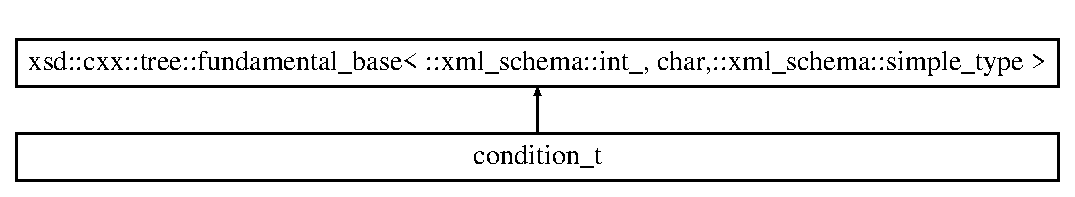
\includegraphics[height=2.000000cm]{classcondition__t}
\end{center}
\end{figure}
\subsection*{Public Member Functions}
\begin{DoxyCompactItemize}
\item 
\hyperlink{classcondition__t_a4c55f19277dbee716114fedde266660d}{condition\-\_\-t} (\-::\hyperlink{namespacexml__schema_acfa24ac68e1a188e7f44c36f7a158bf4}{xml\-\_\-schema\-::int\-\_\-} v)
\item 
\hyperlink{classcondition__t_a5d2e40caebc70537ef8f9e4fb51db4e6}{condition\-\_\-t} (const \-::xercesc\-::\-D\-O\-M\-Element \&e,\-::\hyperlink{namespacexml__schema_a0612287d030cb2732d31a45b258fdc87}{xml\-\_\-schema\-::flags} f=0,\-::\hyperlink{namespacexml__schema_ada9aa30dc722e93ee2ed7243085402a5}{xml\-\_\-schema\-::container} $\ast$c=0)
\item 
\hyperlink{classcondition__t_a804488dd639127e428efa9b953aefd68}{condition\-\_\-t} (const \-::xercesc\-::\-D\-O\-M\-Attr \&a,\-::\hyperlink{namespacexml__schema_a0612287d030cb2732d31a45b258fdc87}{xml\-\_\-schema\-::flags} f=0,\-::\hyperlink{namespacexml__schema_ada9aa30dc722e93ee2ed7243085402a5}{xml\-\_\-schema\-::container} $\ast$c=0)
\item 
\hyperlink{classcondition__t_a2bb3d5ba5abb832f78301c132f1e000d}{condition\-\_\-t} (const \-::std\-::string \&s, const \-::xercesc\-::\-D\-O\-M\-Element $\ast$e,\-::\hyperlink{namespacexml__schema_a0612287d030cb2732d31a45b258fdc87}{xml\-\_\-schema\-::flags} f=0,\-::\hyperlink{namespacexml__schema_ada9aa30dc722e93ee2ed7243085402a5}{xml\-\_\-schema\-::container} $\ast$c=0)
\item 
\hyperlink{classcondition__t_a69909b9e1c95ec62bee98ea62dac883c}{condition\-\_\-t} (const \hyperlink{classcondition__t}{condition\-\_\-t} \&x,\-::\hyperlink{namespacexml__schema_a0612287d030cb2732d31a45b258fdc87}{xml\-\_\-schema\-::flags} f=0,\-::\hyperlink{namespacexml__schema_ada9aa30dc722e93ee2ed7243085402a5}{xml\-\_\-schema\-::container} $\ast$c=0)
\item 
virtual \hyperlink{classcondition__t}{condition\-\_\-t} $\ast$ \hyperlink{classcondition__t_aa04a724a1775f464a7b8e91d3989d298}{\-\_\-clone} (\-::\hyperlink{namespacexml__schema_a0612287d030cb2732d31a45b258fdc87}{xml\-\_\-schema\-::flags} f=0,\-::\hyperlink{namespacexml__schema_ada9aa30dc722e93ee2ed7243085402a5}{xml\-\_\-schema\-::container} $\ast$c=0) const 
\end{DoxyCompactItemize}


\subsection{Constructor \& Destructor Documentation}
\hypertarget{classcondition__t_a4c55f19277dbee716114fedde266660d}{\index{condition\-\_\-t@{condition\-\_\-t}!condition\-\_\-t@{condition\-\_\-t}}
\index{condition\-\_\-t@{condition\-\_\-t}!condition_t@{condition\-\_\-t}}
\subsubsection[{condition\-\_\-t}]{\setlength{\rightskip}{0pt plus 5cm}condition\-\_\-t\-::condition\-\_\-t (
\begin{DoxyParamCaption}
\item[{\-::{\bf xml\-\_\-schema\-::int\-\_\-}}]{v}
\end{DoxyParamCaption}
)}}\label{classcondition__t_a4c55f19277dbee716114fedde266660d}
\hypertarget{classcondition__t_a5d2e40caebc70537ef8f9e4fb51db4e6}{\index{condition\-\_\-t@{condition\-\_\-t}!condition\-\_\-t@{condition\-\_\-t}}
\index{condition\-\_\-t@{condition\-\_\-t}!condition_t@{condition\-\_\-t}}
\subsubsection[{condition\-\_\-t}]{\setlength{\rightskip}{0pt plus 5cm}condition\-\_\-t\-::condition\-\_\-t (
\begin{DoxyParamCaption}
\item[{const \-::xercesc\-::\-D\-O\-M\-Element \&}]{e, }
\item[{\-::{\bf xml\-\_\-schema\-::flags}}]{f = {\ttfamily 0}, }
\item[{\-::{\bf xml\-\_\-schema\-::container} $\ast$}]{c = {\ttfamily 0}}
\end{DoxyParamCaption}
)}}\label{classcondition__t_a5d2e40caebc70537ef8f9e4fb51db4e6}
\hypertarget{classcondition__t_a804488dd639127e428efa9b953aefd68}{\index{condition\-\_\-t@{condition\-\_\-t}!condition\-\_\-t@{condition\-\_\-t}}
\index{condition\-\_\-t@{condition\-\_\-t}!condition_t@{condition\-\_\-t}}
\subsubsection[{condition\-\_\-t}]{\setlength{\rightskip}{0pt plus 5cm}condition\-\_\-t\-::condition\-\_\-t (
\begin{DoxyParamCaption}
\item[{const \-::xercesc\-::\-D\-O\-M\-Attr \&}]{a, }
\item[{\-::{\bf xml\-\_\-schema\-::flags}}]{f = {\ttfamily 0}, }
\item[{\-::{\bf xml\-\_\-schema\-::container} $\ast$}]{c = {\ttfamily 0}}
\end{DoxyParamCaption}
)}}\label{classcondition__t_a804488dd639127e428efa9b953aefd68}
\hypertarget{classcondition__t_a2bb3d5ba5abb832f78301c132f1e000d}{\index{condition\-\_\-t@{condition\-\_\-t}!condition\-\_\-t@{condition\-\_\-t}}
\index{condition\-\_\-t@{condition\-\_\-t}!condition_t@{condition\-\_\-t}}
\subsubsection[{condition\-\_\-t}]{\setlength{\rightskip}{0pt plus 5cm}condition\-\_\-t\-::condition\-\_\-t (
\begin{DoxyParamCaption}
\item[{const \-::std\-::string \&}]{s, }
\item[{const \-::xercesc\-::\-D\-O\-M\-Element $\ast$}]{e, }
\item[{\-::{\bf xml\-\_\-schema\-::flags}}]{f = {\ttfamily 0}, }
\item[{\-::{\bf xml\-\_\-schema\-::container} $\ast$}]{c = {\ttfamily 0}}
\end{DoxyParamCaption}
)}}\label{classcondition__t_a2bb3d5ba5abb832f78301c132f1e000d}
\hypertarget{classcondition__t_a69909b9e1c95ec62bee98ea62dac883c}{\index{condition\-\_\-t@{condition\-\_\-t}!condition\-\_\-t@{condition\-\_\-t}}
\index{condition\-\_\-t@{condition\-\_\-t}!condition_t@{condition\-\_\-t}}
\subsubsection[{condition\-\_\-t}]{\setlength{\rightskip}{0pt plus 5cm}condition\-\_\-t\-::condition\-\_\-t (
\begin{DoxyParamCaption}
\item[{const {\bf condition\-\_\-t} \&}]{x, }
\item[{\-::{\bf xml\-\_\-schema\-::flags}}]{f = {\ttfamily 0}, }
\item[{\-::{\bf xml\-\_\-schema\-::container} $\ast$}]{c = {\ttfamily 0}}
\end{DoxyParamCaption}
)}}\label{classcondition__t_a69909b9e1c95ec62bee98ea62dac883c}


\subsection{Member Function Documentation}
\hypertarget{classcondition__t_aa04a724a1775f464a7b8e91d3989d298}{\index{condition\-\_\-t@{condition\-\_\-t}!\-\_\-clone@{\-\_\-clone}}
\index{\-\_\-clone@{\-\_\-clone}!condition_t@{condition\-\_\-t}}
\subsubsection[{\-\_\-clone}]{\setlength{\rightskip}{0pt plus 5cm}{\bf condition\-\_\-t} $\ast$ condition\-\_\-t\-::\-\_\-clone (
\begin{DoxyParamCaption}
\item[{\-::{\bf xml\-\_\-schema\-::flags}}]{f = {\ttfamily 0}, }
\item[{\-::{\bf xml\-\_\-schema\-::container} $\ast$}]{c = {\ttfamily 0}}
\end{DoxyParamCaption}
) const\hspace{0.3cm}{\ttfamily [virtual]}}}\label{classcondition__t_aa04a724a1775f464a7b8e91d3989d298}


The documentation for this class was generated from the following files\-:\begin{DoxyCompactItemize}
\item 
src/utils/\hyperlink{InputSetting_8h}{Input\-Setting.\-h}\item 
src/utils/\hyperlink{InputSetting_8cpp}{Input\-Setting.\-cpp}\end{DoxyCompactItemize}

\hypertarget{classCuboid}{\section{Cuboid Class Reference}
\label{classCuboid}\index{Cuboid@{Cuboid}}
}


This is a class representing a 3\-D cuboid of particles.  




{\ttfamily \#include $<$Cuboid.\-h$>$}

\subsection*{Public Member Functions}
\begin{DoxyCompactItemize}
\item 
\hyperlink{classCuboid_a1abf60e93d024b7a01ee5b1a48f1f08a}{Cuboid} ()
\item 
\hyperlink{classCuboid_a0ae721afc53bc9c3cb0656a51ce78e8c}{Cuboid} (int height, int width, int \hyperlink{MolSim_8cpp_acb5ba97551079e0b072c62c21d784ac5}{depth}, double distance, double \hyperlink{MolSim_8cpp_aba71f400e3a017e824e2a70435a75542}{mass}, \hyperlink{classutils_1_1Vector}{utils\-::\-Vector}$<$ double, 3 $>$ ori, \hyperlink{classutils_1_1Vector}{utils\-::\-Vector}$<$ double, 3 $>$ start\-Velocity, double mean\-Velocity, int \hyperlink{classCuboid_acd3e5d96f6da99b24468ee9673f9daba}{par\-Type}, double \hyperlink{classCuboid_a3925eb122d69d5938939945a961dc96f}{E\-P\-S\-I\-L\-O\-N}, double \hyperlink{classCuboid_a88c7ddda07e9eb992c8b549ca1f6e827}{S\-I\-G\-M\-A})
\item 
\hyperlink{classutils_1_1Vector}{utils\-::\-Vector}$<$ double, 3 $>$ \& \hyperlink{classCuboid_af02d6e6f4f887e73eab49b2e98d67f9f}{get\-Origin} ()
\item 
\hyperlink{classutils_1_1Vector}{utils\-::\-Vector}$<$ double, 3 $>$ \& \hyperlink{classCuboid_afa1a2f414ad4203d0496779e04cd8cc0}{get\-Start\-V} ()
\item 
std\-::list$<$ \hyperlink{classParticle}{Particle} $>$ \& \hyperlink{classCuboid_ace34581c34e11d770268c653734ebbbf}{get\-Cuboid} ()
\item 
int \hyperlink{classCuboid_a9e2f0ed2b9f4e94623d36f0080c39c60}{get\-Height} ()
\item 
void \hyperlink{classCuboid_a7f18edc87842eb994ba5c4553cf1dfd5}{set\-Height} (double new\-H)
\item 
int \hyperlink{classCuboid_ac339d2ee336e723374b4ac60a008f5a4}{get\-Width} ()
\item 
void \hyperlink{classCuboid_a05ebb7b92f2cf7d99470e0ee37565204}{set\-Width} (double new\-W)
\item 
int \hyperlink{classCuboid_a8a48fe6647e1b6aaefdcdc919d1d60ca}{get\-Depth} ()
\item 
void \hyperlink{classCuboid_ab4a1117474dde7ca1bc7abb17efc60d0}{set\-Depth} (double new\-D)
\item 
double \hyperlink{classCuboid_acce74194a5322bc75176c0b0268dc99e}{get\-Distance} ()
\item 
void \hyperlink{classCuboid_a0118ee212ed9445762e4b66bd049ab29}{set\-Distance} (double new\-D)
\item 
double \hyperlink{classCuboid_a800f78fae7fd092724dc959cfa409894}{get\-Mass} ()
\item 
void \hyperlink{classCuboid_a289a3115396705a7fa2caa8bd873f20d}{set\-Mass} (double new\-M)
\item 
double \hyperlink{classCuboid_ab462bd1cd2a16a29f05b2dd677b600f4}{get\-Mean\-V} ()
\item 
void \hyperlink{classCuboid_a078822ffa44af0b079ed075ad087df26}{set\-Mean\-V} (double new\-V)
\item 
int \hyperlink{classCuboid_a2a324c6cb87afa82b9b933cd3b6bd2cf}{get\-Size} ()
\item 
int \& \hyperlink{classCuboid_ae089a8e4c5ff713c95876d9216e71f92}{get\-Type} ()
\item 
double \& \hyperlink{classCuboid_a3d13a5c0849de7c64ce0076a6f65b995}{get\-Epsilon} ()
\item 
double \& \hyperlink{classCuboid_a4b896bf3579b2b436df51c8f99b75b34}{get\-Sigma} ()
\item 
virtual \hyperlink{classCuboid_aba010c63b64540741c25b5e89b7fabbb}{$\sim$\-Cuboid} ()
\end{DoxyCompactItemize}
\subsection*{Private Attributes}
\begin{DoxyCompactItemize}
\item 
\hyperlink{classutils_1_1Vector}{utils\-::\-Vector}$<$ double, 3 $>$ \hyperlink{classCuboid_ab9fea399762342f5636ea69038606ba1}{origin}
\item 
std\-::list$<$ \hyperlink{classParticle}{Particle} $>$ \hyperlink{classCuboid_a46268af723f395a1cb00533cc8dab6c8}{cub}
\item 
int \hyperlink{classCuboid_a774275af1874294d9d12772eaa7d417a}{c\-Height}
\item 
int \hyperlink{classCuboid_a256b9679e10b33f8e280034a6a7de6e8}{c\-Width}
\item 
int \hyperlink{classCuboid_a9f6823cdaa2bbb8df9ea1a8709a3319c}{c\-Depth}
\item 
double \hyperlink{classCuboid_ad5d539f1c69b321fbbe2dcceef65faba}{h}
\item 
double \hyperlink{classCuboid_a98975bdfb1bd4bbb327167d07d1ffdd4}{m}
\item 
\hyperlink{classutils_1_1Vector}{utils\-::\-Vector}$<$ double, 3 $>$ \hyperlink{classCuboid_a7a95bfb80c884e9f96642c9f7043e9e1}{start\-V}
\item 
double \hyperlink{classCuboid_ab6bb8eb2a87d77e67acea088f6a8ba88}{mean\-V}
\item 
int \hyperlink{classCuboid_acd3e5d96f6da99b24468ee9673f9daba}{par\-Type}
\item 
double \hyperlink{classCuboid_a3925eb122d69d5938939945a961dc96f}{E\-P\-S\-I\-L\-O\-N}
\item 
double \hyperlink{classCuboid_a88c7ddda07e9eb992c8b549ca1f6e827}{S\-I\-G\-M\-A}
\end{DoxyCompactItemize}


\subsection{Detailed Description}
This is a class representing a 3\-D cuboid of particles. 

One cuboid can save a 3\-D set of particles, which are located next to each other. There is no isolated particle in one cuboid. 

\subsection{Constructor \& Destructor Documentation}
\hypertarget{classCuboid_a1abf60e93d024b7a01ee5b1a48f1f08a}{\index{Cuboid@{Cuboid}!Cuboid@{Cuboid}}
\index{Cuboid@{Cuboid}!Cuboid@{Cuboid}}
\subsubsection[{Cuboid}]{\setlength{\rightskip}{0pt plus 5cm}Cuboid\-::\-Cuboid (
\begin{DoxyParamCaption}
{}
\end{DoxyParamCaption}
)}}\label{classCuboid_a1abf60e93d024b7a01ee5b1a48f1f08a}
Default constructor. \hypertarget{classCuboid_a0ae721afc53bc9c3cb0656a51ce78e8c}{\index{Cuboid@{Cuboid}!Cuboid@{Cuboid}}
\index{Cuboid@{Cuboid}!Cuboid@{Cuboid}}
\subsubsection[{Cuboid}]{\setlength{\rightskip}{0pt plus 5cm}Cuboid\-::\-Cuboid (
\begin{DoxyParamCaption}
\item[{int}]{height, }
\item[{int}]{width, }
\item[{int}]{depth, }
\item[{double}]{distance, }
\item[{double}]{mass, }
\item[{{\bf utils\-::\-Vector}$<$ double, 3 $>$}]{ori, }
\item[{{\bf utils\-::\-Vector}$<$ double, 3 $>$}]{start\-Velocity, }
\item[{double}]{mean\-Velocity, }
\item[{int}]{par\-Type, }
\item[{double}]{E\-P\-S\-I\-L\-O\-N, }
\item[{double}]{S\-I\-G\-M\-A}
\end{DoxyParamCaption}
)}}\label{classCuboid_a0ae721afc53bc9c3cb0656a51ce78e8c}
/brief The main constructor.

Constructs a new cuboid with all information needed. 
\begin{DoxyParams}[1]{Parameters}
\mbox{\tt in}  & {\em height} & \hyperlink{classCuboid}{Cuboid}'s height in particles. \\
\hline
\mbox{\tt in}  & {\em width} & \hyperlink{classCuboid}{Cuboid}'s width in particles. \\
\hline
\mbox{\tt in}  & {\em depth} & \hyperlink{classCuboid}{Cuboid}'s depth in particles. \\
\hline
\mbox{\tt in}  & {\em distance} & \hyperlink{classCuboid}{Cuboid}'s mesh width. \\
\hline
\mbox{\tt in}  & {\em mass} & Mass of each particle in cuboid. \\
\hline
\mbox{\tt in}  & {\em ori} & \hyperlink{classCuboid}{Cuboid}'s lower left corner's 3\-D coordinate. \\
\hline
\mbox{\tt in}  & {\em start\-Velocity} & Velocity at the beginning of each particle in cuboid. \\
\hline
\mbox{\tt in}  & {\em mean\-Velocity} & Mean velocity (aka. brownian factor) of each partcile in cuboid. \\
\hline
\mbox{\tt in}  & {\em par\-Type} & \hyperlink{classParticle}{Particle} type of cuboid. \\
\hline
\mbox{\tt in}  & {\em E\-P\-S\-I\-L\-O\-N} & For Lennard Jones Force. \\
\hline
\mbox{\tt in}  & {\em S\-I\-G\-M\-A} & For Lennard Jones Force. \\
\hline
\end{DoxyParams}
\hypertarget{classCuboid_aba010c63b64540741c25b5e89b7fabbb}{\index{Cuboid@{Cuboid}!$\sim$\-Cuboid@{$\sim$\-Cuboid}}
\index{$\sim$\-Cuboid@{$\sim$\-Cuboid}!Cuboid@{Cuboid}}
\subsubsection[{$\sim$\-Cuboid}]{\setlength{\rightskip}{0pt plus 5cm}Cuboid\-::$\sim$\-Cuboid (
\begin{DoxyParamCaption}
{}
\end{DoxyParamCaption}
)\hspace{0.3cm}{\ttfamily [virtual]}}}\label{classCuboid_aba010c63b64540741c25b5e89b7fabbb}


\subsection{Member Function Documentation}
\hypertarget{classCuboid_ace34581c34e11d770268c653734ebbbf}{\index{Cuboid@{Cuboid}!get\-Cuboid@{get\-Cuboid}}
\index{get\-Cuboid@{get\-Cuboid}!Cuboid@{Cuboid}}
\subsubsection[{get\-Cuboid}]{\setlength{\rightskip}{0pt plus 5cm}std\-::list$<$ {\bf Particle} $>$ \& Cuboid\-::get\-Cuboid (
\begin{DoxyParamCaption}
{}
\end{DoxyParamCaption}
)}}\label{classCuboid_ace34581c34e11d770268c653734ebbbf}
\begin{DoxyReturn}{Returns}
\hyperlink{classCuboid}{Cuboid}'s list of particles. 
\end{DoxyReturn}
\hypertarget{classCuboid_a8a48fe6647e1b6aaefdcdc919d1d60ca}{\index{Cuboid@{Cuboid}!get\-Depth@{get\-Depth}}
\index{get\-Depth@{get\-Depth}!Cuboid@{Cuboid}}
\subsubsection[{get\-Depth}]{\setlength{\rightskip}{0pt plus 5cm}int Cuboid\-::get\-Depth (
\begin{DoxyParamCaption}
{}
\end{DoxyParamCaption}
)}}\label{classCuboid_a8a48fe6647e1b6aaefdcdc919d1d60ca}
\begin{DoxyReturn}{Returns}
\hyperlink{classCuboid}{Cuboid}'s depth in particles. 
\end{DoxyReturn}
\hypertarget{classCuboid_acce74194a5322bc75176c0b0268dc99e}{\index{Cuboid@{Cuboid}!get\-Distance@{get\-Distance}}
\index{get\-Distance@{get\-Distance}!Cuboid@{Cuboid}}
\subsubsection[{get\-Distance}]{\setlength{\rightskip}{0pt plus 5cm}double Cuboid\-::get\-Distance (
\begin{DoxyParamCaption}
{}
\end{DoxyParamCaption}
)}}\label{classCuboid_acce74194a5322bc75176c0b0268dc99e}
\begin{DoxyReturn}{Returns}
\hyperlink{classCuboid}{Cuboid}'s mesh width between every 2 particles. 
\end{DoxyReturn}
\hypertarget{classCuboid_a3d13a5c0849de7c64ce0076a6f65b995}{\index{Cuboid@{Cuboid}!get\-Epsilon@{get\-Epsilon}}
\index{get\-Epsilon@{get\-Epsilon}!Cuboid@{Cuboid}}
\subsubsection[{get\-Epsilon}]{\setlength{\rightskip}{0pt plus 5cm}double \& Cuboid\-::get\-Epsilon (
\begin{DoxyParamCaption}
{}
\end{DoxyParamCaption}
)}}\label{classCuboid_a3d13a5c0849de7c64ce0076a6f65b995}
\begin{DoxyReturn}{Returns}
\hyperlink{classCuboid}{Cuboid}'s epsilon for Lennard Jones Force. 
\end{DoxyReturn}
\hypertarget{classCuboid_a9e2f0ed2b9f4e94623d36f0080c39c60}{\index{Cuboid@{Cuboid}!get\-Height@{get\-Height}}
\index{get\-Height@{get\-Height}!Cuboid@{Cuboid}}
\subsubsection[{get\-Height}]{\setlength{\rightskip}{0pt plus 5cm}int Cuboid\-::get\-Height (
\begin{DoxyParamCaption}
{}
\end{DoxyParamCaption}
)}}\label{classCuboid_a9e2f0ed2b9f4e94623d36f0080c39c60}
\begin{DoxyReturn}{Returns}
\hyperlink{classCuboid}{Cuboid}'s height in particles. 
\end{DoxyReturn}
\hypertarget{classCuboid_a800f78fae7fd092724dc959cfa409894}{\index{Cuboid@{Cuboid}!get\-Mass@{get\-Mass}}
\index{get\-Mass@{get\-Mass}!Cuboid@{Cuboid}}
\subsubsection[{get\-Mass}]{\setlength{\rightskip}{0pt plus 5cm}double Cuboid\-::get\-Mass (
\begin{DoxyParamCaption}
{}
\end{DoxyParamCaption}
)}}\label{classCuboid_a800f78fae7fd092724dc959cfa409894}
\begin{DoxyReturn}{Returns}
\hyperlink{classCuboid}{Cuboid}'s mas of every particle. 
\end{DoxyReturn}
\hypertarget{classCuboid_ab462bd1cd2a16a29f05b2dd677b600f4}{\index{Cuboid@{Cuboid}!get\-Mean\-V@{get\-Mean\-V}}
\index{get\-Mean\-V@{get\-Mean\-V}!Cuboid@{Cuboid}}
\subsubsection[{get\-Mean\-V}]{\setlength{\rightskip}{0pt plus 5cm}double Cuboid\-::get\-Mean\-V (
\begin{DoxyParamCaption}
{}
\end{DoxyParamCaption}
)}}\label{classCuboid_ab462bd1cd2a16a29f05b2dd677b600f4}
\begin{DoxyReturn}{Returns}
\hyperlink{classCuboid}{Cuboid}'s mean velocity of every particle. 
\end{DoxyReturn}
\hypertarget{classCuboid_af02d6e6f4f887e73eab49b2e98d67f9f}{\index{Cuboid@{Cuboid}!get\-Origin@{get\-Origin}}
\index{get\-Origin@{get\-Origin}!Cuboid@{Cuboid}}
\subsubsection[{get\-Origin}]{\setlength{\rightskip}{0pt plus 5cm}{\bf utils\-::\-Vector}$<$ double, 3 $>$ \& Cuboid\-::get\-Origin (
\begin{DoxyParamCaption}
{}
\end{DoxyParamCaption}
)}}\label{classCuboid_af02d6e6f4f887e73eab49b2e98d67f9f}
\begin{DoxyReturn}{Returns}
\hyperlink{classCuboid}{Cuboid}'s lower left corner's location. 
\end{DoxyReturn}
\hypertarget{classCuboid_a4b896bf3579b2b436df51c8f99b75b34}{\index{Cuboid@{Cuboid}!get\-Sigma@{get\-Sigma}}
\index{get\-Sigma@{get\-Sigma}!Cuboid@{Cuboid}}
\subsubsection[{get\-Sigma}]{\setlength{\rightskip}{0pt plus 5cm}double \& Cuboid\-::get\-Sigma (
\begin{DoxyParamCaption}
{}
\end{DoxyParamCaption}
)}}\label{classCuboid_a4b896bf3579b2b436df51c8f99b75b34}
\begin{DoxyReturn}{Returns}
\hyperlink{classCuboid}{Cuboid}'s sigma for Lennard Jones Force. 
\end{DoxyReturn}
\hypertarget{classCuboid_a2a324c6cb87afa82b9b933cd3b6bd2cf}{\index{Cuboid@{Cuboid}!get\-Size@{get\-Size}}
\index{get\-Size@{get\-Size}!Cuboid@{Cuboid}}
\subsubsection[{get\-Size}]{\setlength{\rightskip}{0pt plus 5cm}int Cuboid\-::get\-Size (
\begin{DoxyParamCaption}
{}
\end{DoxyParamCaption}
)}}\label{classCuboid_a2a324c6cb87afa82b9b933cd3b6bd2cf}
\begin{DoxyReturn}{Returns}
\hyperlink{classCuboid}{Cuboid}'s size in particles. 
\end{DoxyReturn}
\hypertarget{classCuboid_afa1a2f414ad4203d0496779e04cd8cc0}{\index{Cuboid@{Cuboid}!get\-Start\-V@{get\-Start\-V}}
\index{get\-Start\-V@{get\-Start\-V}!Cuboid@{Cuboid}}
\subsubsection[{get\-Start\-V}]{\setlength{\rightskip}{0pt plus 5cm}{\bf utils\-::\-Vector}$<$ double, 3 $>$ \& Cuboid\-::get\-Start\-V (
\begin{DoxyParamCaption}
{}
\end{DoxyParamCaption}
)}}\label{classCuboid_afa1a2f414ad4203d0496779e04cd8cc0}
\begin{DoxyReturn}{Returns}
Velocity at the beginning of each particle in cuboid. 
\end{DoxyReturn}
\hypertarget{classCuboid_ae089a8e4c5ff713c95876d9216e71f92}{\index{Cuboid@{Cuboid}!get\-Type@{get\-Type}}
\index{get\-Type@{get\-Type}!Cuboid@{Cuboid}}
\subsubsection[{get\-Type}]{\setlength{\rightskip}{0pt plus 5cm}int \& Cuboid\-::get\-Type (
\begin{DoxyParamCaption}
{}
\end{DoxyParamCaption}
)}}\label{classCuboid_ae089a8e4c5ff713c95876d9216e71f92}
\begin{DoxyReturn}{Returns}
\hyperlink{classCuboid}{Cuboid}'s particle type. 
\end{DoxyReturn}
\hypertarget{classCuboid_ac339d2ee336e723374b4ac60a008f5a4}{\index{Cuboid@{Cuboid}!get\-Width@{get\-Width}}
\index{get\-Width@{get\-Width}!Cuboid@{Cuboid}}
\subsubsection[{get\-Width}]{\setlength{\rightskip}{0pt plus 5cm}int Cuboid\-::get\-Width (
\begin{DoxyParamCaption}
{}
\end{DoxyParamCaption}
)}}\label{classCuboid_ac339d2ee336e723374b4ac60a008f5a4}
\begin{DoxyReturn}{Returns}
\hyperlink{classCuboid}{Cuboid}'s width in particles. 
\end{DoxyReturn}
\hypertarget{classCuboid_ab4a1117474dde7ca1bc7abb17efc60d0}{\index{Cuboid@{Cuboid}!set\-Depth@{set\-Depth}}
\index{set\-Depth@{set\-Depth}!Cuboid@{Cuboid}}
\subsubsection[{set\-Depth}]{\setlength{\rightskip}{0pt plus 5cm}void Cuboid\-::set\-Depth (
\begin{DoxyParamCaption}
\item[{double}]{new\-D}
\end{DoxyParamCaption}
)}}\label{classCuboid_ab4a1117474dde7ca1bc7abb17efc60d0}
Setter for depth. 
\begin{DoxyParams}[1]{Parameters}
\mbox{\tt in}  & {\em new\-D} & The new value of width to be set. \\
\hline
\end{DoxyParams}
\hypertarget{classCuboid_a0118ee212ed9445762e4b66bd049ab29}{\index{Cuboid@{Cuboid}!set\-Distance@{set\-Distance}}
\index{set\-Distance@{set\-Distance}!Cuboid@{Cuboid}}
\subsubsection[{set\-Distance}]{\setlength{\rightskip}{0pt plus 5cm}void Cuboid\-::set\-Distance (
\begin{DoxyParamCaption}
\item[{double}]{new\-D}
\end{DoxyParamCaption}
)}}\label{classCuboid_a0118ee212ed9445762e4b66bd049ab29}
Setter for mesh width between every 2 particles. 
\begin{DoxyParams}[1]{Parameters}
\mbox{\tt in}  & {\em new\-D} & The new value of mesh width to be set. \\
\hline
\end{DoxyParams}
\hypertarget{classCuboid_a7f18edc87842eb994ba5c4553cf1dfd5}{\index{Cuboid@{Cuboid}!set\-Height@{set\-Height}}
\index{set\-Height@{set\-Height}!Cuboid@{Cuboid}}
\subsubsection[{set\-Height}]{\setlength{\rightskip}{0pt plus 5cm}void Cuboid\-::set\-Height (
\begin{DoxyParamCaption}
\item[{double}]{new\-H}
\end{DoxyParamCaption}
)}}\label{classCuboid_a7f18edc87842eb994ba5c4553cf1dfd5}
Setter for height. 
\begin{DoxyParams}[1]{Parameters}
\mbox{\tt in}  & {\em new\-H} & The new value of height to be set. \\
\hline
\end{DoxyParams}
\hypertarget{classCuboid_a289a3115396705a7fa2caa8bd873f20d}{\index{Cuboid@{Cuboid}!set\-Mass@{set\-Mass}}
\index{set\-Mass@{set\-Mass}!Cuboid@{Cuboid}}
\subsubsection[{set\-Mass}]{\setlength{\rightskip}{0pt plus 5cm}void Cuboid\-::set\-Mass (
\begin{DoxyParamCaption}
\item[{double}]{new\-M}
\end{DoxyParamCaption}
)}}\label{classCuboid_a289a3115396705a7fa2caa8bd873f20d}
Setter for mass every particle. 
\begin{DoxyParams}[1]{Parameters}
\mbox{\tt in}  & {\em new\-M} & The new value of mass to be set. \\
\hline
\end{DoxyParams}
\hypertarget{classCuboid_a078822ffa44af0b079ed075ad087df26}{\index{Cuboid@{Cuboid}!set\-Mean\-V@{set\-Mean\-V}}
\index{set\-Mean\-V@{set\-Mean\-V}!Cuboid@{Cuboid}}
\subsubsection[{set\-Mean\-V}]{\setlength{\rightskip}{0pt plus 5cm}void Cuboid\-::set\-Mean\-V (
\begin{DoxyParamCaption}
\item[{double}]{new\-V}
\end{DoxyParamCaption}
)}}\label{classCuboid_a078822ffa44af0b079ed075ad087df26}
Setter for mean velocity of every particle. 
\begin{DoxyParams}[1]{Parameters}
\mbox{\tt in}  & {\em new\-V} & The new value of mean velocity to be set. \\
\hline
\end{DoxyParams}
\hypertarget{classCuboid_a05ebb7b92f2cf7d99470e0ee37565204}{\index{Cuboid@{Cuboid}!set\-Width@{set\-Width}}
\index{set\-Width@{set\-Width}!Cuboid@{Cuboid}}
\subsubsection[{set\-Width}]{\setlength{\rightskip}{0pt plus 5cm}void Cuboid\-::set\-Width (
\begin{DoxyParamCaption}
\item[{double}]{new\-W}
\end{DoxyParamCaption}
)}}\label{classCuboid_a05ebb7b92f2cf7d99470e0ee37565204}
Setter for width. 
\begin{DoxyParams}[1]{Parameters}
\mbox{\tt in}  & {\em new\-W} & The new value of width to be set. \\
\hline
\end{DoxyParams}


\subsection{Member Data Documentation}
\hypertarget{classCuboid_a9f6823cdaa2bbb8df9ea1a8709a3319c}{\index{Cuboid@{Cuboid}!c\-Depth@{c\-Depth}}
\index{c\-Depth@{c\-Depth}!Cuboid@{Cuboid}}
\subsubsection[{c\-Depth}]{\setlength{\rightskip}{0pt plus 5cm}int Cuboid\-::c\-Depth\hspace{0.3cm}{\ttfamily [private]}}}\label{classCuboid_a9f6823cdaa2bbb8df9ea1a8709a3319c}
\hyperlink{classCuboid}{Cuboid}'s depth (measured in particles). \hypertarget{classCuboid_a774275af1874294d9d12772eaa7d417a}{\index{Cuboid@{Cuboid}!c\-Height@{c\-Height}}
\index{c\-Height@{c\-Height}!Cuboid@{Cuboid}}
\subsubsection[{c\-Height}]{\setlength{\rightskip}{0pt plus 5cm}int Cuboid\-::c\-Height\hspace{0.3cm}{\ttfamily [private]}}}\label{classCuboid_a774275af1874294d9d12772eaa7d417a}
\hyperlink{classCuboid}{Cuboid}'s height (measured in particles). \hypertarget{classCuboid_a46268af723f395a1cb00533cc8dab6c8}{\index{Cuboid@{Cuboid}!cub@{cub}}
\index{cub@{cub}!Cuboid@{Cuboid}}
\subsubsection[{cub}]{\setlength{\rightskip}{0pt plus 5cm}std\-::list$<${\bf Particle}$>$ Cuboid\-::cub\hspace{0.3cm}{\ttfamily [private]}}}\label{classCuboid_a46268af723f395a1cb00533cc8dab6c8}
The particles of a cuboid are saved in one single list. \hypertarget{classCuboid_a256b9679e10b33f8e280034a6a7de6e8}{\index{Cuboid@{Cuboid}!c\-Width@{c\-Width}}
\index{c\-Width@{c\-Width}!Cuboid@{Cuboid}}
\subsubsection[{c\-Width}]{\setlength{\rightskip}{0pt plus 5cm}int Cuboid\-::c\-Width\hspace{0.3cm}{\ttfamily [private]}}}\label{classCuboid_a256b9679e10b33f8e280034a6a7de6e8}
\hyperlink{classCuboid}{Cuboid}'s width (measured in particles). \hypertarget{classCuboid_a3925eb122d69d5938939945a961dc96f}{\index{Cuboid@{Cuboid}!E\-P\-S\-I\-L\-O\-N@{E\-P\-S\-I\-L\-O\-N}}
\index{E\-P\-S\-I\-L\-O\-N@{E\-P\-S\-I\-L\-O\-N}!Cuboid@{Cuboid}}
\subsubsection[{E\-P\-S\-I\-L\-O\-N}]{\setlength{\rightskip}{0pt plus 5cm}double Cuboid\-::\-E\-P\-S\-I\-L\-O\-N\hspace{0.3cm}{\ttfamily [private]}}}\label{classCuboid_a3925eb122d69d5938939945a961dc96f}
For Lennard Jones Force. \hypertarget{classCuboid_ad5d539f1c69b321fbbe2dcceef65faba}{\index{Cuboid@{Cuboid}!h@{h}}
\index{h@{h}!Cuboid@{Cuboid}}
\subsubsection[{h}]{\setlength{\rightskip}{0pt plus 5cm}double Cuboid\-::h\hspace{0.3cm}{\ttfamily [private]}}}\label{classCuboid_ad5d539f1c69b321fbbe2dcceef65faba}
The mesh width between every 2 particles. \hypertarget{classCuboid_a98975bdfb1bd4bbb327167d07d1ffdd4}{\index{Cuboid@{Cuboid}!m@{m}}
\index{m@{m}!Cuboid@{Cuboid}}
\subsubsection[{m}]{\setlength{\rightskip}{0pt plus 5cm}double Cuboid\-::m\hspace{0.3cm}{\ttfamily [private]}}}\label{classCuboid_a98975bdfb1bd4bbb327167d07d1ffdd4}
The mass of each particle in cuboid. \hypertarget{classCuboid_ab6bb8eb2a87d77e67acea088f6a8ba88}{\index{Cuboid@{Cuboid}!mean\-V@{mean\-V}}
\index{mean\-V@{mean\-V}!Cuboid@{Cuboid}}
\subsubsection[{mean\-V}]{\setlength{\rightskip}{0pt plus 5cm}double Cuboid\-::mean\-V\hspace{0.3cm}{\ttfamily [private]}}}\label{classCuboid_ab6bb8eb2a87d77e67acea088f6a8ba88}
The mean velocity (aka. brownian factor) of each particle. \hypertarget{classCuboid_ab9fea399762342f5636ea69038606ba1}{\index{Cuboid@{Cuboid}!origin@{origin}}
\index{origin@{origin}!Cuboid@{Cuboid}}
\subsubsection[{origin}]{\setlength{\rightskip}{0pt plus 5cm}{\bf utils\-::\-Vector}$<$double, 3$>$ Cuboid\-::origin\hspace{0.3cm}{\ttfamily [private]}}}\label{classCuboid_ab9fea399762342f5636ea69038606ba1}
A 3\-D vector indicating the location of the lower left corner of a cuboid. \hypertarget{classCuboid_acd3e5d96f6da99b24468ee9673f9daba}{\index{Cuboid@{Cuboid}!par\-Type@{par\-Type}}
\index{par\-Type@{par\-Type}!Cuboid@{Cuboid}}
\subsubsection[{par\-Type}]{\setlength{\rightskip}{0pt plus 5cm}int Cuboid\-::par\-Type\hspace{0.3cm}{\ttfamily [private]}}}\label{classCuboid_acd3e5d96f6da99b24468ee9673f9daba}
\hypertarget{classCuboid_a88c7ddda07e9eb992c8b549ca1f6e827}{\index{Cuboid@{Cuboid}!S\-I\-G\-M\-A@{S\-I\-G\-M\-A}}
\index{S\-I\-G\-M\-A@{S\-I\-G\-M\-A}!Cuboid@{Cuboid}}
\subsubsection[{S\-I\-G\-M\-A}]{\setlength{\rightskip}{0pt plus 5cm}double Cuboid\-::\-S\-I\-G\-M\-A\hspace{0.3cm}{\ttfamily [private]}}}\label{classCuboid_a88c7ddda07e9eb992c8b549ca1f6e827}
For Lennard Jones Force. \hypertarget{classCuboid_a7a95bfb80c884e9f96642c9f7043e9e1}{\index{Cuboid@{Cuboid}!start\-V@{start\-V}}
\index{start\-V@{start\-V}!Cuboid@{Cuboid}}
\subsubsection[{start\-V}]{\setlength{\rightskip}{0pt plus 5cm}{\bf utils\-::\-Vector}$<$double, 3$>$ Cuboid\-::start\-V\hspace{0.3cm}{\ttfamily [private]}}}\label{classCuboid_a7a95bfb80c884e9f96642c9f7043e9e1}
The velocity at the beginning of each particle. 

The documentation for this class was generated from the following files\-:\begin{DoxyCompactItemize}
\item 
src/\hyperlink{Cuboid_8h}{Cuboid.\-h}\item 
src/\hyperlink{Cuboid_8cpp}{Cuboid.\-cpp}\end{DoxyCompactItemize}

\hypertarget{classcuboid__t}{\section{cuboid\-\_\-t Class Reference}
\label{classcuboid__t}\index{cuboid\-\_\-t@{cuboid\-\_\-t}}
}


{\ttfamily \#include $<$Input\-Cuboids.\-h$>$}

Inheritance diagram for cuboid\-\_\-t\-:\begin{figure}[H]
\begin{center}
\leavevmode
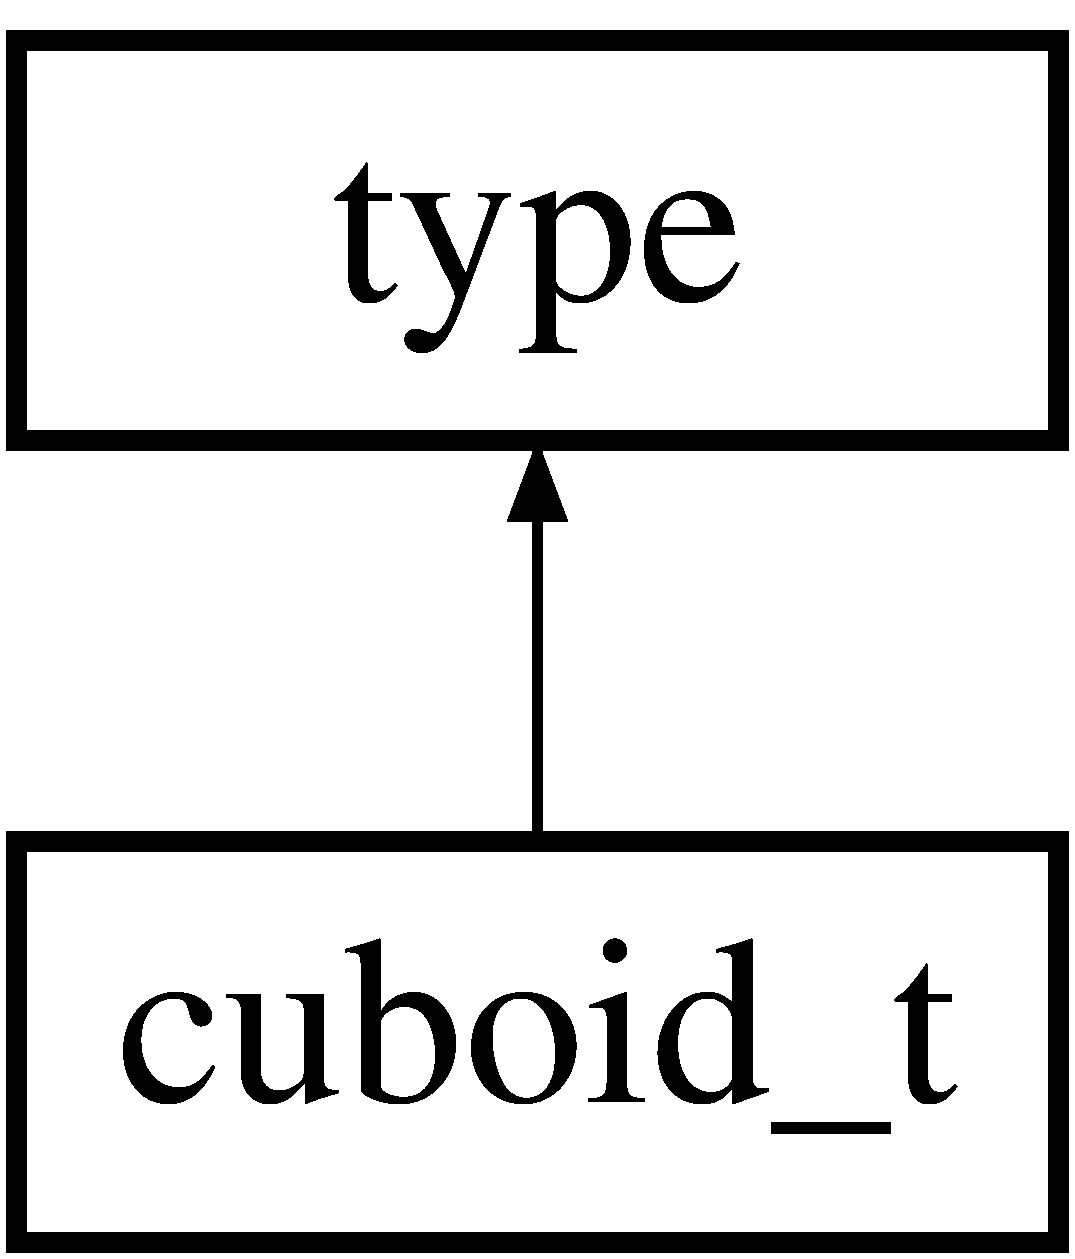
\includegraphics[height=2.000000cm]{classcuboid__t}
\end{center}
\end{figure}
\subsection*{Public Types}
\begin{DoxyCompactItemize}
\item 
typedef \-::\hyperlink{namespacexml__schema_a69bfaf24f63a8c18ebd8e21db6b343df}{xml\-\_\-schema\-::decimal} \hyperlink{classcuboid__t_a5759759b1b9e3029ff36c7f20d9213dc}{mesh\-Width\-\_\-type}
\item 
typedef \\*
\-::xsd\-::cxx\-::tree\-::traits\\*
$<$ \hyperlink{classcuboid__t_a5759759b1b9e3029ff36c7f20d9213dc}{mesh\-Width\-\_\-type}, char,\-::xsd\-::cxx\-::tree\-::schema\-\_\-type\-::decimal $>$ \hyperlink{classcuboid__t_a7407ec25461e872616716771073fdd6b}{mesh\-Width\-\_\-traits}
\item 
typedef \-::\hyperlink{namespacexml__schema_a69bfaf24f63a8c18ebd8e21db6b343df}{xml\-\_\-schema\-::decimal} \hyperlink{classcuboid__t_a365536fb1db29c6ef0da234297763d61}{mass\-\_\-type}
\item 
typedef \\*
\-::xsd\-::cxx\-::tree\-::traits\\*
$<$ \hyperlink{classcuboid__t_a365536fb1db29c6ef0da234297763d61}{mass\-\_\-type}, char,\-::xsd\-::cxx\-::tree\-::schema\-\_\-type\-::decimal $>$ \hyperlink{classcuboid__t_a3414ba3ff63f2e3abac4ec2f5ff7932d}{mass\-\_\-traits}
\item 
typedef \-::\hyperlink{namespacexml__schema_a69bfaf24f63a8c18ebd8e21db6b343df}{xml\-\_\-schema\-::decimal} \hyperlink{classcuboid__t_aea1381b8b1cca3f677ae4a28b29cbe2a}{mean\-V\-\_\-type}
\item 
typedef \\*
\-::xsd\-::cxx\-::tree\-::traits\\*
$<$ \hyperlink{classcuboid__t_aea1381b8b1cca3f677ae4a28b29cbe2a}{mean\-V\-\_\-type}, char,\-::xsd\-::cxx\-::tree\-::schema\-\_\-type\-::decimal $>$ \hyperlink{classcuboid__t_ad39df1b8bcb315153993a8993dc0828c}{mean\-V\-\_\-traits}
\item 
typedef \-::\hyperlink{namespacexml__schema_acfa24ac68e1a188e7f44c36f7a158bf4}{xml\-\_\-schema\-::int\-\_\-} \hyperlink{classcuboid__t_a162caafd069fa127809bb2d573c752c5}{par\-Type\-C\-\_\-type}
\item 
typedef \\*
\-::xsd\-::cxx\-::tree\-::traits\\*
$<$ \hyperlink{classcuboid__t_a162caafd069fa127809bb2d573c752c5}{par\-Type\-C\-\_\-type}, char $>$ \hyperlink{classcuboid__t_adc1cedef5964dbd3021fa55ee6271554}{par\-Type\-C\-\_\-traits}
\item 
typedef \-::\hyperlink{namespacexml__schema_a69bfaf24f63a8c18ebd8e21db6b343df}{xml\-\_\-schema\-::decimal} \hyperlink{classcuboid__t_ac4a981a7963b1b2105d448cf42ab1230}{epsilon\-\_\-type}
\item 
typedef \\*
\-::xsd\-::cxx\-::tree\-::traits\\*
$<$ \hyperlink{classcuboid__t_ac4a981a7963b1b2105d448cf42ab1230}{epsilon\-\_\-type}, char,\-::xsd\-::cxx\-::tree\-::schema\-\_\-type\-::decimal $>$ \hyperlink{classcuboid__t_a909ff9ef57adeb2edaa27cda6e531c44}{epsilon\-\_\-traits}
\item 
typedef \-::\hyperlink{namespacexml__schema_a69bfaf24f63a8c18ebd8e21db6b343df}{xml\-\_\-schema\-::decimal} \hyperlink{classcuboid__t_ae1de9c7b1d2b2a9098de31c546c0ff83}{sigma\-\_\-type}
\item 
typedef \\*
\-::xsd\-::cxx\-::tree\-::traits\\*
$<$ \hyperlink{classcuboid__t_ae1de9c7b1d2b2a9098de31c546c0ff83}{sigma\-\_\-type}, char,\-::xsd\-::cxx\-::tree\-::schema\-\_\-type\-::decimal $>$ \hyperlink{classcuboid__t_a40e03084467dcf27dc74ece86086b047}{sigma\-\_\-traits}
\item 
typedef \-::\hyperlink{classori__t}{ori\-\_\-t} \hyperlink{classcuboid__t_a20d67505efc00dc82947ce881aec1e76}{origin\-Vector\-\_\-type}
\item 
typedef \\*
\-::xsd\-::cxx\-::tree\-::traits\\*
$<$ \hyperlink{classcuboid__t_a20d67505efc00dc82947ce881aec1e76}{origin\-Vector\-\_\-type}, char $>$ \hyperlink{classcuboid__t_a88fa351b02759f012d3dc7cabd2097b8}{origin\-Vector\-\_\-traits}
\item 
typedef \-::\hyperlink{classstartV__t}{start\-V\-\_\-t} \hyperlink{classcuboid__t_a7b9bd2a7888abc4b08f6f4e91ac9a81f}{start\-Velocity\-\_\-type}
\item 
typedef \\*
\-::xsd\-::cxx\-::tree\-::traits\\*
$<$ \hyperlink{classcuboid__t_a7b9bd2a7888abc4b08f6f4e91ac9a81f}{start\-Velocity\-\_\-type}, char $>$ \hyperlink{classcuboid__t_a0d43837eb6423a21e59b6f36012b244a}{start\-Velocity\-\_\-traits}
\item 
typedef \-::\hyperlink{classsize3D__t}{size3\-D\-\_\-t} \hyperlink{classcuboid__t_abf130ab4ed6d70047bb193a41283ec28}{size3\-D\-\_\-type}
\item 
typedef \\*
\-::xsd\-::cxx\-::tree\-::traits\\*
$<$ \hyperlink{classcuboid__t_abf130ab4ed6d70047bb193a41283ec28}{size3\-D\-\_\-type}, char $>$ \hyperlink{classcuboid__t_a8f449274f0802c092d0abd4f45ea1cdc}{size3\-D\-\_\-traits}
\end{DoxyCompactItemize}
\subsection*{Public Member Functions}
\begin{DoxyCompactItemize}
\item 
const \hyperlink{classcuboid__t_a5759759b1b9e3029ff36c7f20d9213dc}{mesh\-Width\-\_\-type} \& \hyperlink{classcuboid__t_ad2dc45a3a6fe778095f17a48afe33dd2}{mesh\-Width} () const 
\item 
\hyperlink{classcuboid__t_a5759759b1b9e3029ff36c7f20d9213dc}{mesh\-Width\-\_\-type} \& \hyperlink{classcuboid__t_aa3f7e2375cf92229b67e10134034201d}{mesh\-Width} ()
\item 
void \hyperlink{classcuboid__t_a18109f7e2b099c9e965b8d78f02a9e02}{mesh\-Width} (const \hyperlink{classcuboid__t_a5759759b1b9e3029ff36c7f20d9213dc}{mesh\-Width\-\_\-type} \&x)
\item 
const \hyperlink{classcuboid__t_a365536fb1db29c6ef0da234297763d61}{mass\-\_\-type} \& \hyperlink{classcuboid__t_ad3c09a2fd500ca03fa5bd0a8e70de5bf}{mass} () const 
\item 
\hyperlink{classcuboid__t_a365536fb1db29c6ef0da234297763d61}{mass\-\_\-type} \& \hyperlink{classcuboid__t_a886b32175330faa8cf5b3b4a6d5f962b}{mass} ()
\item 
void \hyperlink{classcuboid__t_a819aa170a5430d8e58e8c8bd21690655}{mass} (const \hyperlink{classcuboid__t_a365536fb1db29c6ef0da234297763d61}{mass\-\_\-type} \&x)
\item 
const \hyperlink{classcuboid__t_aea1381b8b1cca3f677ae4a28b29cbe2a}{mean\-V\-\_\-type} \& \hyperlink{classcuboid__t_a91b634b6561023a36e4da1957394c3fb}{mean\-V} () const 
\item 
\hyperlink{classcuboid__t_aea1381b8b1cca3f677ae4a28b29cbe2a}{mean\-V\-\_\-type} \& \hyperlink{classcuboid__t_aa4d3de66ea96cd11a2402e8d68b49b98}{mean\-V} ()
\item 
void \hyperlink{classcuboid__t_a58ad62869916aaef7c04fe400b39e4c0}{mean\-V} (const \hyperlink{classcuboid__t_aea1381b8b1cca3f677ae4a28b29cbe2a}{mean\-V\-\_\-type} \&x)
\item 
const \hyperlink{classcuboid__t_a162caafd069fa127809bb2d573c752c5}{par\-Type\-C\-\_\-type} \& \hyperlink{classcuboid__t_a923b33f2683e0df94603c429547be912}{par\-Type\-C} () const 
\item 
\hyperlink{classcuboid__t_a162caafd069fa127809bb2d573c752c5}{par\-Type\-C\-\_\-type} \& \hyperlink{classcuboid__t_aa70a57aa669fdf89f3ed1d464c9c9cf7}{par\-Type\-C} ()
\item 
void \hyperlink{classcuboid__t_a7eac87c8db11eb19bc4873220d366831}{par\-Type\-C} (const \hyperlink{classcuboid__t_a162caafd069fa127809bb2d573c752c5}{par\-Type\-C\-\_\-type} \&x)
\item 
const \hyperlink{classcuboid__t_ac4a981a7963b1b2105d448cf42ab1230}{epsilon\-\_\-type} \& \hyperlink{classcuboid__t_acd8d400db715227486dd790cd6d94b6e}{epsilon} () const 
\item 
\hyperlink{classcuboid__t_ac4a981a7963b1b2105d448cf42ab1230}{epsilon\-\_\-type} \& \hyperlink{classcuboid__t_af1d9a282a756b593b4fa62beb59fdc82}{epsilon} ()
\item 
void \hyperlink{classcuboid__t_acdacc4d702d49a86c06cc2b1578d8bab}{epsilon} (const \hyperlink{classcuboid__t_ac4a981a7963b1b2105d448cf42ab1230}{epsilon\-\_\-type} \&x)
\item 
const \hyperlink{classcuboid__t_ae1de9c7b1d2b2a9098de31c546c0ff83}{sigma\-\_\-type} \& \hyperlink{classcuboid__t_ae13a7e732dc3c3ae94d8aaffba7ee617}{sigma} () const 
\item 
\hyperlink{classcuboid__t_ae1de9c7b1d2b2a9098de31c546c0ff83}{sigma\-\_\-type} \& \hyperlink{classcuboid__t_a0a25741d3a40cffb89c4b8f62fd5b302}{sigma} ()
\item 
void \hyperlink{classcuboid__t_aa8ad42d35fb7d27f8e3a476e75e02b40}{sigma} (const \hyperlink{classcuboid__t_ae1de9c7b1d2b2a9098de31c546c0ff83}{sigma\-\_\-type} \&x)
\item 
const \hyperlink{classcuboid__t_a20d67505efc00dc82947ce881aec1e76}{origin\-Vector\-\_\-type} \& \hyperlink{classcuboid__t_afe1995f8cfc6ba9a2297f40ff819cbf4}{origin\-Vector} () const 
\item 
\hyperlink{classcuboid__t_a20d67505efc00dc82947ce881aec1e76}{origin\-Vector\-\_\-type} \& \hyperlink{classcuboid__t_a4694704c1be9385729b17f5c5ab76c4d}{origin\-Vector} ()
\item 
void \hyperlink{classcuboid__t_a4e4a379837eb1a37609203e890977a60}{origin\-Vector} (const \hyperlink{classcuboid__t_a20d67505efc00dc82947ce881aec1e76}{origin\-Vector\-\_\-type} \&x)
\item 
void \hyperlink{classcuboid__t_a202c8b82852eed4c25905e251105079d}{origin\-Vector} (\-::std\-::auto\-\_\-ptr$<$ \hyperlink{classcuboid__t_a20d67505efc00dc82947ce881aec1e76}{origin\-Vector\-\_\-type} $>$ p)
\item 
const \hyperlink{classcuboid__t_a7b9bd2a7888abc4b08f6f4e91ac9a81f}{start\-Velocity\-\_\-type} \& \hyperlink{classcuboid__t_aa2d8956335c51c61b3d24655faaef8e9}{start\-Velocity} () const 
\item 
\hyperlink{classcuboid__t_a7b9bd2a7888abc4b08f6f4e91ac9a81f}{start\-Velocity\-\_\-type} \& \hyperlink{classcuboid__t_a985354621466cf976351d5ae91c8e54d}{start\-Velocity} ()
\item 
void \hyperlink{classcuboid__t_a7fd31641814ea206932d025a8b1c30ca}{start\-Velocity} (const \hyperlink{classcuboid__t_a7b9bd2a7888abc4b08f6f4e91ac9a81f}{start\-Velocity\-\_\-type} \&x)
\item 
void \hyperlink{classcuboid__t_a7cacb68eea7d510a128dc8428a11c13b}{start\-Velocity} (\-::std\-::auto\-\_\-ptr$<$ \hyperlink{classcuboid__t_a7b9bd2a7888abc4b08f6f4e91ac9a81f}{start\-Velocity\-\_\-type} $>$ p)
\item 
const \hyperlink{classcuboid__t_abf130ab4ed6d70047bb193a41283ec28}{size3\-D\-\_\-type} \& \hyperlink{classcuboid__t_ad814d59fb91adb1c63a17c41bd37abce}{size3\-D} () const 
\item 
\hyperlink{classcuboid__t_abf130ab4ed6d70047bb193a41283ec28}{size3\-D\-\_\-type} \& \hyperlink{classcuboid__t_ac8a91327ce480ee6c17408cced64cceb}{size3\-D} ()
\item 
void \hyperlink{classcuboid__t_a9a87bc74d77d5acb4d47993fd26bdcc2}{size3\-D} (const \hyperlink{classcuboid__t_abf130ab4ed6d70047bb193a41283ec28}{size3\-D\-\_\-type} \&x)
\item 
void \hyperlink{classcuboid__t_aa26d6df9982c5fa7ca418f577e4e8730}{size3\-D} (\-::std\-::auto\-\_\-ptr$<$ \hyperlink{classcuboid__t_abf130ab4ed6d70047bb193a41283ec28}{size3\-D\-\_\-type} $>$ p)
\item 
\hyperlink{classcuboid__t_addac6142a0729945fd67babbcac59aec}{cuboid\-\_\-t} (const \hyperlink{classcuboid__t_a5759759b1b9e3029ff36c7f20d9213dc}{mesh\-Width\-\_\-type} \&, const \hyperlink{classcuboid__t_a365536fb1db29c6ef0da234297763d61}{mass\-\_\-type} \&, const \hyperlink{classcuboid__t_aea1381b8b1cca3f677ae4a28b29cbe2a}{mean\-V\-\_\-type} \&, const \hyperlink{classcuboid__t_a162caafd069fa127809bb2d573c752c5}{par\-Type\-C\-\_\-type} \&, const \hyperlink{classcuboid__t_ac4a981a7963b1b2105d448cf42ab1230}{epsilon\-\_\-type} \&, const \hyperlink{classcuboid__t_ae1de9c7b1d2b2a9098de31c546c0ff83}{sigma\-\_\-type} \&, const \hyperlink{classcuboid__t_a20d67505efc00dc82947ce881aec1e76}{origin\-Vector\-\_\-type} \&, const \hyperlink{classcuboid__t_a7b9bd2a7888abc4b08f6f4e91ac9a81f}{start\-Velocity\-\_\-type} \&, const \hyperlink{classcuboid__t_abf130ab4ed6d70047bb193a41283ec28}{size3\-D\-\_\-type} \&)
\item 
\hyperlink{classcuboid__t_a862bcca4943b2c27a5f5edfd361bb4a1}{cuboid\-\_\-t} (const \hyperlink{classcuboid__t_a5759759b1b9e3029ff36c7f20d9213dc}{mesh\-Width\-\_\-type} \&, const \hyperlink{classcuboid__t_a365536fb1db29c6ef0da234297763d61}{mass\-\_\-type} \&, const \hyperlink{classcuboid__t_aea1381b8b1cca3f677ae4a28b29cbe2a}{mean\-V\-\_\-type} \&, const \hyperlink{classcuboid__t_a162caafd069fa127809bb2d573c752c5}{par\-Type\-C\-\_\-type} \&, const \hyperlink{classcuboid__t_ac4a981a7963b1b2105d448cf42ab1230}{epsilon\-\_\-type} \&, const \hyperlink{classcuboid__t_ae1de9c7b1d2b2a9098de31c546c0ff83}{sigma\-\_\-type} \&,\-::std\-::auto\-\_\-ptr$<$ \hyperlink{classcuboid__t_a20d67505efc00dc82947ce881aec1e76}{origin\-Vector\-\_\-type} $>$ \&,\-::std\-::auto\-\_\-ptr$<$ \hyperlink{classcuboid__t_a7b9bd2a7888abc4b08f6f4e91ac9a81f}{start\-Velocity\-\_\-type} $>$ \&,\-::std\-::auto\-\_\-ptr$<$ \hyperlink{classcuboid__t_abf130ab4ed6d70047bb193a41283ec28}{size3\-D\-\_\-type} $>$ \&)
\item 
\hyperlink{classcuboid__t_afa1b7588ca19d8c5d00fb8c5dcf92bc8}{cuboid\-\_\-t} (const \-::xercesc\-::\-D\-O\-M\-Element \&e,\-::\hyperlink{namespacexml__schema_a0612287d030cb2732d31a45b258fdc87}{xml\-\_\-schema\-::flags} f=0,\-::\hyperlink{namespacexml__schema_ada9aa30dc722e93ee2ed7243085402a5}{xml\-\_\-schema\-::container} $\ast$c=0)
\item 
\hyperlink{classcuboid__t_a1574d539277176b5fff09a374c142c90}{cuboid\-\_\-t} (const \hyperlink{classcuboid__t}{cuboid\-\_\-t} \&x,\-::\hyperlink{namespacexml__schema_a0612287d030cb2732d31a45b258fdc87}{xml\-\_\-schema\-::flags} f=0,\-::\hyperlink{namespacexml__schema_ada9aa30dc722e93ee2ed7243085402a5}{xml\-\_\-schema\-::container} $\ast$c=0)
\item 
virtual \hyperlink{classcuboid__t}{cuboid\-\_\-t} $\ast$ \hyperlink{classcuboid__t_aa31bc17c300c78f7c15b08d60bbdefbf}{\-\_\-clone} (\-::\hyperlink{namespacexml__schema_a0612287d030cb2732d31a45b258fdc87}{xml\-\_\-schema\-::flags} f=0,\-::\hyperlink{namespacexml__schema_ada9aa30dc722e93ee2ed7243085402a5}{xml\-\_\-schema\-::container} $\ast$c=0) const 
\item 
virtual \hyperlink{classcuboid__t_ad45791533f3643e2e2f565801c0ca20a}{$\sim$cuboid\-\_\-t} ()
\end{DoxyCompactItemize}
\subsection*{Protected Member Functions}
\begin{DoxyCompactItemize}
\item 
void \hyperlink{classcuboid__t_ab79e4219bf9a205aff7cbbda1207d138}{parse} (\-::xsd\-::cxx\-::xml\-::dom\-::parser$<$ char $>$ \&,\-::\hyperlink{namespacexml__schema_a0612287d030cb2732d31a45b258fdc87}{xml\-\_\-schema\-::flags})
\end{DoxyCompactItemize}
\subsection*{Protected Attributes}
\begin{DoxyCompactItemize}
\item 
\-::xsd\-::cxx\-::tree\-::one\\*
$<$ \hyperlink{classcuboid__t_a5759759b1b9e3029ff36c7f20d9213dc}{mesh\-Width\-\_\-type} $>$ \hyperlink{classcuboid__t_af31779bcbd1ff3844623c658f633a8aa}{mesh\-Width\-\_\-}
\item 
\-::xsd\-::cxx\-::tree\-::one$<$ \hyperlink{classcuboid__t_a365536fb1db29c6ef0da234297763d61}{mass\-\_\-type} $>$ \hyperlink{classcuboid__t_a9c7dd176b3732eb61362f104fe51e4b8}{mass\-\_\-}
\item 
\-::xsd\-::cxx\-::tree\-::one$<$ \hyperlink{classcuboid__t_aea1381b8b1cca3f677ae4a28b29cbe2a}{mean\-V\-\_\-type} $>$ \hyperlink{classcuboid__t_a3d83a46d242a523fb10095e9025abddf}{mean\-V\-\_\-}
\item 
\-::xsd\-::cxx\-::tree\-::one\\*
$<$ \hyperlink{classcuboid__t_a162caafd069fa127809bb2d573c752c5}{par\-Type\-C\-\_\-type} $>$ \hyperlink{classcuboid__t_a0ce3a150a7054afaab0b4cfb600b5920}{par\-Type\-C\-\_\-}
\item 
\-::xsd\-::cxx\-::tree\-::one\\*
$<$ \hyperlink{classcuboid__t_ac4a981a7963b1b2105d448cf42ab1230}{epsilon\-\_\-type} $>$ \hyperlink{classcuboid__t_a89f568a5a27be873e0f482d708e31e3d}{epsilon\-\_\-}
\item 
\-::xsd\-::cxx\-::tree\-::one$<$ \hyperlink{classcuboid__t_ae1de9c7b1d2b2a9098de31c546c0ff83}{sigma\-\_\-type} $>$ \hyperlink{classcuboid__t_ad68ee2b884c2bdec543177f9b2027021}{sigma\-\_\-}
\item 
\-::xsd\-::cxx\-::tree\-::one\\*
$<$ \hyperlink{classcuboid__t_a20d67505efc00dc82947ce881aec1e76}{origin\-Vector\-\_\-type} $>$ \hyperlink{classcuboid__t_aa74b198d17ccc0d095655adf9cfa312b}{origin\-Vector\-\_\-}
\item 
\-::xsd\-::cxx\-::tree\-::one\\*
$<$ \hyperlink{classcuboid__t_a7b9bd2a7888abc4b08f6f4e91ac9a81f}{start\-Velocity\-\_\-type} $>$ \hyperlink{classcuboid__t_a0720684b94609a0c60088e2535cc2c67}{start\-Velocity\-\_\-}
\item 
\-::xsd\-::cxx\-::tree\-::one\\*
$<$ \hyperlink{classcuboid__t_abf130ab4ed6d70047bb193a41283ec28}{size3\-D\-\_\-type} $>$ \hyperlink{classcuboid__t_afccbf21e84c29d7cc05cadf8d5945856}{size3\-D\-\_\-}
\end{DoxyCompactItemize}


\subsection{Member Typedef Documentation}
\hypertarget{classcuboid__t_a909ff9ef57adeb2edaa27cda6e531c44}{\index{cuboid\-\_\-t@{cuboid\-\_\-t}!epsilon\-\_\-traits@{epsilon\-\_\-traits}}
\index{epsilon\-\_\-traits@{epsilon\-\_\-traits}!cuboid_t@{cuboid\-\_\-t}}
\subsubsection[{epsilon\-\_\-traits}]{\setlength{\rightskip}{0pt plus 5cm}typedef \-::xsd\-::cxx\-::tree\-::traits$<$ {\bf epsilon\-\_\-type}, char, \-::xsd\-::cxx\-::tree\-::schema\-\_\-type\-::decimal $>$ {\bf cuboid\-\_\-t\-::epsilon\-\_\-traits}}}\label{classcuboid__t_a909ff9ef57adeb2edaa27cda6e531c44}
\hypertarget{classcuboid__t_ac4a981a7963b1b2105d448cf42ab1230}{\index{cuboid\-\_\-t@{cuboid\-\_\-t}!epsilon\-\_\-type@{epsilon\-\_\-type}}
\index{epsilon\-\_\-type@{epsilon\-\_\-type}!cuboid_t@{cuboid\-\_\-t}}
\subsubsection[{epsilon\-\_\-type}]{\setlength{\rightskip}{0pt plus 5cm}typedef \-::{\bf xml\-\_\-schema\-::decimal} {\bf cuboid\-\_\-t\-::epsilon\-\_\-type}}}\label{classcuboid__t_ac4a981a7963b1b2105d448cf42ab1230}
\hypertarget{classcuboid__t_a3414ba3ff63f2e3abac4ec2f5ff7932d}{\index{cuboid\-\_\-t@{cuboid\-\_\-t}!mass\-\_\-traits@{mass\-\_\-traits}}
\index{mass\-\_\-traits@{mass\-\_\-traits}!cuboid_t@{cuboid\-\_\-t}}
\subsubsection[{mass\-\_\-traits}]{\setlength{\rightskip}{0pt plus 5cm}typedef \-::xsd\-::cxx\-::tree\-::traits$<$ {\bf mass\-\_\-type}, char, \-::xsd\-::cxx\-::tree\-::schema\-\_\-type\-::decimal $>$ {\bf cuboid\-\_\-t\-::mass\-\_\-traits}}}\label{classcuboid__t_a3414ba3ff63f2e3abac4ec2f5ff7932d}
\hypertarget{classcuboid__t_a365536fb1db29c6ef0da234297763d61}{\index{cuboid\-\_\-t@{cuboid\-\_\-t}!mass\-\_\-type@{mass\-\_\-type}}
\index{mass\-\_\-type@{mass\-\_\-type}!cuboid_t@{cuboid\-\_\-t}}
\subsubsection[{mass\-\_\-type}]{\setlength{\rightskip}{0pt plus 5cm}typedef \-::{\bf xml\-\_\-schema\-::decimal} {\bf cuboid\-\_\-t\-::mass\-\_\-type}}}\label{classcuboid__t_a365536fb1db29c6ef0da234297763d61}
\hypertarget{classcuboid__t_ad39df1b8bcb315153993a8993dc0828c}{\index{cuboid\-\_\-t@{cuboid\-\_\-t}!mean\-V\-\_\-traits@{mean\-V\-\_\-traits}}
\index{mean\-V\-\_\-traits@{mean\-V\-\_\-traits}!cuboid_t@{cuboid\-\_\-t}}
\subsubsection[{mean\-V\-\_\-traits}]{\setlength{\rightskip}{0pt plus 5cm}typedef \-::xsd\-::cxx\-::tree\-::traits$<$ {\bf mean\-V\-\_\-type}, char, \-::xsd\-::cxx\-::tree\-::schema\-\_\-type\-::decimal $>$ {\bf cuboid\-\_\-t\-::mean\-V\-\_\-traits}}}\label{classcuboid__t_ad39df1b8bcb315153993a8993dc0828c}
\hypertarget{classcuboid__t_aea1381b8b1cca3f677ae4a28b29cbe2a}{\index{cuboid\-\_\-t@{cuboid\-\_\-t}!mean\-V\-\_\-type@{mean\-V\-\_\-type}}
\index{mean\-V\-\_\-type@{mean\-V\-\_\-type}!cuboid_t@{cuboid\-\_\-t}}
\subsubsection[{mean\-V\-\_\-type}]{\setlength{\rightskip}{0pt plus 5cm}typedef \-::{\bf xml\-\_\-schema\-::decimal} {\bf cuboid\-\_\-t\-::mean\-V\-\_\-type}}}\label{classcuboid__t_aea1381b8b1cca3f677ae4a28b29cbe2a}
\hypertarget{classcuboid__t_a7407ec25461e872616716771073fdd6b}{\index{cuboid\-\_\-t@{cuboid\-\_\-t}!mesh\-Width\-\_\-traits@{mesh\-Width\-\_\-traits}}
\index{mesh\-Width\-\_\-traits@{mesh\-Width\-\_\-traits}!cuboid_t@{cuboid\-\_\-t}}
\subsubsection[{mesh\-Width\-\_\-traits}]{\setlength{\rightskip}{0pt plus 5cm}typedef \-::xsd\-::cxx\-::tree\-::traits$<$ {\bf mesh\-Width\-\_\-type}, char, \-::xsd\-::cxx\-::tree\-::schema\-\_\-type\-::decimal $>$ {\bf cuboid\-\_\-t\-::mesh\-Width\-\_\-traits}}}\label{classcuboid__t_a7407ec25461e872616716771073fdd6b}
\hypertarget{classcuboid__t_a5759759b1b9e3029ff36c7f20d9213dc}{\index{cuboid\-\_\-t@{cuboid\-\_\-t}!mesh\-Width\-\_\-type@{mesh\-Width\-\_\-type}}
\index{mesh\-Width\-\_\-type@{mesh\-Width\-\_\-type}!cuboid_t@{cuboid\-\_\-t}}
\subsubsection[{mesh\-Width\-\_\-type}]{\setlength{\rightskip}{0pt plus 5cm}typedef \-::{\bf xml\-\_\-schema\-::decimal} {\bf cuboid\-\_\-t\-::mesh\-Width\-\_\-type}}}\label{classcuboid__t_a5759759b1b9e3029ff36c7f20d9213dc}
\hypertarget{classcuboid__t_a88fa351b02759f012d3dc7cabd2097b8}{\index{cuboid\-\_\-t@{cuboid\-\_\-t}!origin\-Vector\-\_\-traits@{origin\-Vector\-\_\-traits}}
\index{origin\-Vector\-\_\-traits@{origin\-Vector\-\_\-traits}!cuboid_t@{cuboid\-\_\-t}}
\subsubsection[{origin\-Vector\-\_\-traits}]{\setlength{\rightskip}{0pt plus 5cm}typedef \-::xsd\-::cxx\-::tree\-::traits$<$ {\bf origin\-Vector\-\_\-type}, char $>$ {\bf cuboid\-\_\-t\-::origin\-Vector\-\_\-traits}}}\label{classcuboid__t_a88fa351b02759f012d3dc7cabd2097b8}
\hypertarget{classcuboid__t_a20d67505efc00dc82947ce881aec1e76}{\index{cuboid\-\_\-t@{cuboid\-\_\-t}!origin\-Vector\-\_\-type@{origin\-Vector\-\_\-type}}
\index{origin\-Vector\-\_\-type@{origin\-Vector\-\_\-type}!cuboid_t@{cuboid\-\_\-t}}
\subsubsection[{origin\-Vector\-\_\-type}]{\setlength{\rightskip}{0pt plus 5cm}typedef \-::{\bf ori\-\_\-t} {\bf cuboid\-\_\-t\-::origin\-Vector\-\_\-type}}}\label{classcuboid__t_a20d67505efc00dc82947ce881aec1e76}
\hypertarget{classcuboid__t_adc1cedef5964dbd3021fa55ee6271554}{\index{cuboid\-\_\-t@{cuboid\-\_\-t}!par\-Type\-C\-\_\-traits@{par\-Type\-C\-\_\-traits}}
\index{par\-Type\-C\-\_\-traits@{par\-Type\-C\-\_\-traits}!cuboid_t@{cuboid\-\_\-t}}
\subsubsection[{par\-Type\-C\-\_\-traits}]{\setlength{\rightskip}{0pt plus 5cm}typedef \-::xsd\-::cxx\-::tree\-::traits$<$ {\bf par\-Type\-C\-\_\-type}, char $>$ {\bf cuboid\-\_\-t\-::par\-Type\-C\-\_\-traits}}}\label{classcuboid__t_adc1cedef5964dbd3021fa55ee6271554}
\hypertarget{classcuboid__t_a162caafd069fa127809bb2d573c752c5}{\index{cuboid\-\_\-t@{cuboid\-\_\-t}!par\-Type\-C\-\_\-type@{par\-Type\-C\-\_\-type}}
\index{par\-Type\-C\-\_\-type@{par\-Type\-C\-\_\-type}!cuboid_t@{cuboid\-\_\-t}}
\subsubsection[{par\-Type\-C\-\_\-type}]{\setlength{\rightskip}{0pt plus 5cm}typedef \-::{\bf xml\-\_\-schema\-::int\-\_\-} {\bf cuboid\-\_\-t\-::par\-Type\-C\-\_\-type}}}\label{classcuboid__t_a162caafd069fa127809bb2d573c752c5}
\hypertarget{classcuboid__t_a40e03084467dcf27dc74ece86086b047}{\index{cuboid\-\_\-t@{cuboid\-\_\-t}!sigma\-\_\-traits@{sigma\-\_\-traits}}
\index{sigma\-\_\-traits@{sigma\-\_\-traits}!cuboid_t@{cuboid\-\_\-t}}
\subsubsection[{sigma\-\_\-traits}]{\setlength{\rightskip}{0pt plus 5cm}typedef \-::xsd\-::cxx\-::tree\-::traits$<$ {\bf sigma\-\_\-type}, char, \-::xsd\-::cxx\-::tree\-::schema\-\_\-type\-::decimal $>$ {\bf cuboid\-\_\-t\-::sigma\-\_\-traits}}}\label{classcuboid__t_a40e03084467dcf27dc74ece86086b047}
\hypertarget{classcuboid__t_ae1de9c7b1d2b2a9098de31c546c0ff83}{\index{cuboid\-\_\-t@{cuboid\-\_\-t}!sigma\-\_\-type@{sigma\-\_\-type}}
\index{sigma\-\_\-type@{sigma\-\_\-type}!cuboid_t@{cuboid\-\_\-t}}
\subsubsection[{sigma\-\_\-type}]{\setlength{\rightskip}{0pt plus 5cm}typedef \-::{\bf xml\-\_\-schema\-::decimal} {\bf cuboid\-\_\-t\-::sigma\-\_\-type}}}\label{classcuboid__t_ae1de9c7b1d2b2a9098de31c546c0ff83}
\hypertarget{classcuboid__t_a8f449274f0802c092d0abd4f45ea1cdc}{\index{cuboid\-\_\-t@{cuboid\-\_\-t}!size3\-D\-\_\-traits@{size3\-D\-\_\-traits}}
\index{size3\-D\-\_\-traits@{size3\-D\-\_\-traits}!cuboid_t@{cuboid\-\_\-t}}
\subsubsection[{size3\-D\-\_\-traits}]{\setlength{\rightskip}{0pt plus 5cm}typedef \-::xsd\-::cxx\-::tree\-::traits$<$ {\bf size3\-D\-\_\-type}, char $>$ {\bf cuboid\-\_\-t\-::size3\-D\-\_\-traits}}}\label{classcuboid__t_a8f449274f0802c092d0abd4f45ea1cdc}
\hypertarget{classcuboid__t_abf130ab4ed6d70047bb193a41283ec28}{\index{cuboid\-\_\-t@{cuboid\-\_\-t}!size3\-D\-\_\-type@{size3\-D\-\_\-type}}
\index{size3\-D\-\_\-type@{size3\-D\-\_\-type}!cuboid_t@{cuboid\-\_\-t}}
\subsubsection[{size3\-D\-\_\-type}]{\setlength{\rightskip}{0pt plus 5cm}typedef \-::{\bf size3\-D\-\_\-t} {\bf cuboid\-\_\-t\-::size3\-D\-\_\-type}}}\label{classcuboid__t_abf130ab4ed6d70047bb193a41283ec28}
\hypertarget{classcuboid__t_a0d43837eb6423a21e59b6f36012b244a}{\index{cuboid\-\_\-t@{cuboid\-\_\-t}!start\-Velocity\-\_\-traits@{start\-Velocity\-\_\-traits}}
\index{start\-Velocity\-\_\-traits@{start\-Velocity\-\_\-traits}!cuboid_t@{cuboid\-\_\-t}}
\subsubsection[{start\-Velocity\-\_\-traits}]{\setlength{\rightskip}{0pt plus 5cm}typedef \-::xsd\-::cxx\-::tree\-::traits$<$ {\bf start\-Velocity\-\_\-type}, char $>$ {\bf cuboid\-\_\-t\-::start\-Velocity\-\_\-traits}}}\label{classcuboid__t_a0d43837eb6423a21e59b6f36012b244a}
\hypertarget{classcuboid__t_a7b9bd2a7888abc4b08f6f4e91ac9a81f}{\index{cuboid\-\_\-t@{cuboid\-\_\-t}!start\-Velocity\-\_\-type@{start\-Velocity\-\_\-type}}
\index{start\-Velocity\-\_\-type@{start\-Velocity\-\_\-type}!cuboid_t@{cuboid\-\_\-t}}
\subsubsection[{start\-Velocity\-\_\-type}]{\setlength{\rightskip}{0pt plus 5cm}typedef \-::{\bf start\-V\-\_\-t} {\bf cuboid\-\_\-t\-::start\-Velocity\-\_\-type}}}\label{classcuboid__t_a7b9bd2a7888abc4b08f6f4e91ac9a81f}


\subsection{Constructor \& Destructor Documentation}
\hypertarget{classcuboid__t_addac6142a0729945fd67babbcac59aec}{\index{cuboid\-\_\-t@{cuboid\-\_\-t}!cuboid\-\_\-t@{cuboid\-\_\-t}}
\index{cuboid\-\_\-t@{cuboid\-\_\-t}!cuboid_t@{cuboid\-\_\-t}}
\subsubsection[{cuboid\-\_\-t}]{\setlength{\rightskip}{0pt plus 5cm}cuboid\-\_\-t\-::cuboid\-\_\-t (
\begin{DoxyParamCaption}
\item[{const {\bf mesh\-Width\-\_\-type} \&}]{mesh\-Width, }
\item[{const {\bf mass\-\_\-type} \&}]{mass, }
\item[{const {\bf mean\-V\-\_\-type} \&}]{mean\-V, }
\item[{const {\bf par\-Type\-C\-\_\-type} \&}]{par\-Type\-C, }
\item[{const {\bf epsilon\-\_\-type} \&}]{epsilon, }
\item[{const {\bf sigma\-\_\-type} \&}]{sigma, }
\item[{const {\bf origin\-Vector\-\_\-type} \&}]{origin\-Vector, }
\item[{const {\bf start\-Velocity\-\_\-type} \&}]{start\-Velocity, }
\item[{const {\bf size3\-D\-\_\-type} \&}]{size3\-D}
\end{DoxyParamCaption}
)}}\label{classcuboid__t_addac6142a0729945fd67babbcac59aec}
\hypertarget{classcuboid__t_a862bcca4943b2c27a5f5edfd361bb4a1}{\index{cuboid\-\_\-t@{cuboid\-\_\-t}!cuboid\-\_\-t@{cuboid\-\_\-t}}
\index{cuboid\-\_\-t@{cuboid\-\_\-t}!cuboid_t@{cuboid\-\_\-t}}
\subsubsection[{cuboid\-\_\-t}]{\setlength{\rightskip}{0pt plus 5cm}cuboid\-\_\-t\-::cuboid\-\_\-t (
\begin{DoxyParamCaption}
\item[{const {\bf mesh\-Width\-\_\-type} \&}]{mesh\-Width, }
\item[{const {\bf mass\-\_\-type} \&}]{mass, }
\item[{const {\bf mean\-V\-\_\-type} \&}]{mean\-V, }
\item[{const {\bf par\-Type\-C\-\_\-type} \&}]{par\-Type\-C, }
\item[{const {\bf epsilon\-\_\-type} \&}]{epsilon, }
\item[{const {\bf sigma\-\_\-type} \&}]{sigma, }
\item[{\-::std\-::auto\-\_\-ptr$<$ {\bf origin\-Vector\-\_\-type} $>$ \&}]{origin\-Vector, }
\item[{\-::std\-::auto\-\_\-ptr$<$ {\bf start\-Velocity\-\_\-type} $>$ \&}]{start\-Velocity, }
\item[{\-::std\-::auto\-\_\-ptr$<$ {\bf size3\-D\-\_\-type} $>$ \&}]{size3\-D}
\end{DoxyParamCaption}
)}}\label{classcuboid__t_a862bcca4943b2c27a5f5edfd361bb4a1}
\hypertarget{classcuboid__t_afa1b7588ca19d8c5d00fb8c5dcf92bc8}{\index{cuboid\-\_\-t@{cuboid\-\_\-t}!cuboid\-\_\-t@{cuboid\-\_\-t}}
\index{cuboid\-\_\-t@{cuboid\-\_\-t}!cuboid_t@{cuboid\-\_\-t}}
\subsubsection[{cuboid\-\_\-t}]{\setlength{\rightskip}{0pt plus 5cm}cuboid\-\_\-t\-::cuboid\-\_\-t (
\begin{DoxyParamCaption}
\item[{const \-::xercesc\-::\-D\-O\-M\-Element \&}]{e, }
\item[{\-::{\bf xml\-\_\-schema\-::flags}}]{f = {\ttfamily 0}, }
\item[{\-::{\bf xml\-\_\-schema\-::container} $\ast$}]{c = {\ttfamily 0}}
\end{DoxyParamCaption}
)}}\label{classcuboid__t_afa1b7588ca19d8c5d00fb8c5dcf92bc8}
\hypertarget{classcuboid__t_a1574d539277176b5fff09a374c142c90}{\index{cuboid\-\_\-t@{cuboid\-\_\-t}!cuboid\-\_\-t@{cuboid\-\_\-t}}
\index{cuboid\-\_\-t@{cuboid\-\_\-t}!cuboid_t@{cuboid\-\_\-t}}
\subsubsection[{cuboid\-\_\-t}]{\setlength{\rightskip}{0pt plus 5cm}cuboid\-\_\-t\-::cuboid\-\_\-t (
\begin{DoxyParamCaption}
\item[{const {\bf cuboid\-\_\-t} \&}]{x, }
\item[{\-::{\bf xml\-\_\-schema\-::flags}}]{f = {\ttfamily 0}, }
\item[{\-::{\bf xml\-\_\-schema\-::container} $\ast$}]{c = {\ttfamily 0}}
\end{DoxyParamCaption}
)}}\label{classcuboid__t_a1574d539277176b5fff09a374c142c90}
\hypertarget{classcuboid__t_ad45791533f3643e2e2f565801c0ca20a}{\index{cuboid\-\_\-t@{cuboid\-\_\-t}!$\sim$cuboid\-\_\-t@{$\sim$cuboid\-\_\-t}}
\index{$\sim$cuboid\-\_\-t@{$\sim$cuboid\-\_\-t}!cuboid_t@{cuboid\-\_\-t}}
\subsubsection[{$\sim$cuboid\-\_\-t}]{\setlength{\rightskip}{0pt plus 5cm}cuboid\-\_\-t\-::$\sim$cuboid\-\_\-t (
\begin{DoxyParamCaption}
{}
\end{DoxyParamCaption}
)\hspace{0.3cm}{\ttfamily [virtual]}}}\label{classcuboid__t_ad45791533f3643e2e2f565801c0ca20a}


\subsection{Member Function Documentation}
\hypertarget{classcuboid__t_aa31bc17c300c78f7c15b08d60bbdefbf}{\index{cuboid\-\_\-t@{cuboid\-\_\-t}!\-\_\-clone@{\-\_\-clone}}
\index{\-\_\-clone@{\-\_\-clone}!cuboid_t@{cuboid\-\_\-t}}
\subsubsection[{\-\_\-clone}]{\setlength{\rightskip}{0pt plus 5cm}{\bf cuboid\-\_\-t} $\ast$ cuboid\-\_\-t\-::\-\_\-clone (
\begin{DoxyParamCaption}
\item[{\-::{\bf xml\-\_\-schema\-::flags}}]{f = {\ttfamily 0}, }
\item[{\-::{\bf xml\-\_\-schema\-::container} $\ast$}]{c = {\ttfamily 0}}
\end{DoxyParamCaption}
) const\hspace{0.3cm}{\ttfamily [virtual]}}}\label{classcuboid__t_aa31bc17c300c78f7c15b08d60bbdefbf}
\hypertarget{classcuboid__t_acd8d400db715227486dd790cd6d94b6e}{\index{cuboid\-\_\-t@{cuboid\-\_\-t}!epsilon@{epsilon}}
\index{epsilon@{epsilon}!cuboid_t@{cuboid\-\_\-t}}
\subsubsection[{epsilon}]{\setlength{\rightskip}{0pt plus 5cm}const {\bf cuboid\-\_\-t\-::epsilon\-\_\-type} \& cuboid\-\_\-t\-::epsilon (
\begin{DoxyParamCaption}
{}
\end{DoxyParamCaption}
) const}}\label{classcuboid__t_acd8d400db715227486dd790cd6d94b6e}
\hypertarget{classcuboid__t_af1d9a282a756b593b4fa62beb59fdc82}{\index{cuboid\-\_\-t@{cuboid\-\_\-t}!epsilon@{epsilon}}
\index{epsilon@{epsilon}!cuboid_t@{cuboid\-\_\-t}}
\subsubsection[{epsilon}]{\setlength{\rightskip}{0pt plus 5cm}{\bf cuboid\-\_\-t\-::epsilon\-\_\-type} \& cuboid\-\_\-t\-::epsilon (
\begin{DoxyParamCaption}
{}
\end{DoxyParamCaption}
)}}\label{classcuboid__t_af1d9a282a756b593b4fa62beb59fdc82}
\hypertarget{classcuboid__t_acdacc4d702d49a86c06cc2b1578d8bab}{\index{cuboid\-\_\-t@{cuboid\-\_\-t}!epsilon@{epsilon}}
\index{epsilon@{epsilon}!cuboid_t@{cuboid\-\_\-t}}
\subsubsection[{epsilon}]{\setlength{\rightskip}{0pt plus 5cm}void cuboid\-\_\-t\-::epsilon (
\begin{DoxyParamCaption}
\item[{const {\bf epsilon\-\_\-type} \&}]{x}
\end{DoxyParamCaption}
)}}\label{classcuboid__t_acdacc4d702d49a86c06cc2b1578d8bab}
\hypertarget{classcuboid__t_ad3c09a2fd500ca03fa5bd0a8e70de5bf}{\index{cuboid\-\_\-t@{cuboid\-\_\-t}!mass@{mass}}
\index{mass@{mass}!cuboid_t@{cuboid\-\_\-t}}
\subsubsection[{mass}]{\setlength{\rightskip}{0pt plus 5cm}const {\bf cuboid\-\_\-t\-::mass\-\_\-type} \& cuboid\-\_\-t\-::mass (
\begin{DoxyParamCaption}
{}
\end{DoxyParamCaption}
) const}}\label{classcuboid__t_ad3c09a2fd500ca03fa5bd0a8e70de5bf}
\hypertarget{classcuboid__t_a886b32175330faa8cf5b3b4a6d5f962b}{\index{cuboid\-\_\-t@{cuboid\-\_\-t}!mass@{mass}}
\index{mass@{mass}!cuboid_t@{cuboid\-\_\-t}}
\subsubsection[{mass}]{\setlength{\rightskip}{0pt plus 5cm}{\bf cuboid\-\_\-t\-::mass\-\_\-type} \& cuboid\-\_\-t\-::mass (
\begin{DoxyParamCaption}
{}
\end{DoxyParamCaption}
)}}\label{classcuboid__t_a886b32175330faa8cf5b3b4a6d5f962b}
\hypertarget{classcuboid__t_a819aa170a5430d8e58e8c8bd21690655}{\index{cuboid\-\_\-t@{cuboid\-\_\-t}!mass@{mass}}
\index{mass@{mass}!cuboid_t@{cuboid\-\_\-t}}
\subsubsection[{mass}]{\setlength{\rightskip}{0pt plus 5cm}void cuboid\-\_\-t\-::mass (
\begin{DoxyParamCaption}
\item[{const {\bf mass\-\_\-type} \&}]{x}
\end{DoxyParamCaption}
)}}\label{classcuboid__t_a819aa170a5430d8e58e8c8bd21690655}
\hypertarget{classcuboid__t_a91b634b6561023a36e4da1957394c3fb}{\index{cuboid\-\_\-t@{cuboid\-\_\-t}!mean\-V@{mean\-V}}
\index{mean\-V@{mean\-V}!cuboid_t@{cuboid\-\_\-t}}
\subsubsection[{mean\-V}]{\setlength{\rightskip}{0pt plus 5cm}const {\bf cuboid\-\_\-t\-::mean\-V\-\_\-type} \& cuboid\-\_\-t\-::mean\-V (
\begin{DoxyParamCaption}
{}
\end{DoxyParamCaption}
) const}}\label{classcuboid__t_a91b634b6561023a36e4da1957394c3fb}
\hypertarget{classcuboid__t_aa4d3de66ea96cd11a2402e8d68b49b98}{\index{cuboid\-\_\-t@{cuboid\-\_\-t}!mean\-V@{mean\-V}}
\index{mean\-V@{mean\-V}!cuboid_t@{cuboid\-\_\-t}}
\subsubsection[{mean\-V}]{\setlength{\rightskip}{0pt plus 5cm}{\bf cuboid\-\_\-t\-::mean\-V\-\_\-type} \& cuboid\-\_\-t\-::mean\-V (
\begin{DoxyParamCaption}
{}
\end{DoxyParamCaption}
)}}\label{classcuboid__t_aa4d3de66ea96cd11a2402e8d68b49b98}
\hypertarget{classcuboid__t_a58ad62869916aaef7c04fe400b39e4c0}{\index{cuboid\-\_\-t@{cuboid\-\_\-t}!mean\-V@{mean\-V}}
\index{mean\-V@{mean\-V}!cuboid_t@{cuboid\-\_\-t}}
\subsubsection[{mean\-V}]{\setlength{\rightskip}{0pt plus 5cm}void cuboid\-\_\-t\-::mean\-V (
\begin{DoxyParamCaption}
\item[{const {\bf mean\-V\-\_\-type} \&}]{x}
\end{DoxyParamCaption}
)}}\label{classcuboid__t_a58ad62869916aaef7c04fe400b39e4c0}
\hypertarget{classcuboid__t_ad2dc45a3a6fe778095f17a48afe33dd2}{\index{cuboid\-\_\-t@{cuboid\-\_\-t}!mesh\-Width@{mesh\-Width}}
\index{mesh\-Width@{mesh\-Width}!cuboid_t@{cuboid\-\_\-t}}
\subsubsection[{mesh\-Width}]{\setlength{\rightskip}{0pt plus 5cm}const {\bf cuboid\-\_\-t\-::mesh\-Width\-\_\-type} \& cuboid\-\_\-t\-::mesh\-Width (
\begin{DoxyParamCaption}
{}
\end{DoxyParamCaption}
) const}}\label{classcuboid__t_ad2dc45a3a6fe778095f17a48afe33dd2}
\hypertarget{classcuboid__t_aa3f7e2375cf92229b67e10134034201d}{\index{cuboid\-\_\-t@{cuboid\-\_\-t}!mesh\-Width@{mesh\-Width}}
\index{mesh\-Width@{mesh\-Width}!cuboid_t@{cuboid\-\_\-t}}
\subsubsection[{mesh\-Width}]{\setlength{\rightskip}{0pt plus 5cm}{\bf cuboid\-\_\-t\-::mesh\-Width\-\_\-type} \& cuboid\-\_\-t\-::mesh\-Width (
\begin{DoxyParamCaption}
{}
\end{DoxyParamCaption}
)}}\label{classcuboid__t_aa3f7e2375cf92229b67e10134034201d}
\hypertarget{classcuboid__t_a18109f7e2b099c9e965b8d78f02a9e02}{\index{cuboid\-\_\-t@{cuboid\-\_\-t}!mesh\-Width@{mesh\-Width}}
\index{mesh\-Width@{mesh\-Width}!cuboid_t@{cuboid\-\_\-t}}
\subsubsection[{mesh\-Width}]{\setlength{\rightskip}{0pt plus 5cm}void cuboid\-\_\-t\-::mesh\-Width (
\begin{DoxyParamCaption}
\item[{const {\bf mesh\-Width\-\_\-type} \&}]{x}
\end{DoxyParamCaption}
)}}\label{classcuboid__t_a18109f7e2b099c9e965b8d78f02a9e02}
\hypertarget{classcuboid__t_afe1995f8cfc6ba9a2297f40ff819cbf4}{\index{cuboid\-\_\-t@{cuboid\-\_\-t}!origin\-Vector@{origin\-Vector}}
\index{origin\-Vector@{origin\-Vector}!cuboid_t@{cuboid\-\_\-t}}
\subsubsection[{origin\-Vector}]{\setlength{\rightskip}{0pt plus 5cm}const {\bf cuboid\-\_\-t\-::origin\-Vector\-\_\-type} \& cuboid\-\_\-t\-::origin\-Vector (
\begin{DoxyParamCaption}
{}
\end{DoxyParamCaption}
) const}}\label{classcuboid__t_afe1995f8cfc6ba9a2297f40ff819cbf4}
\hypertarget{classcuboid__t_a4694704c1be9385729b17f5c5ab76c4d}{\index{cuboid\-\_\-t@{cuboid\-\_\-t}!origin\-Vector@{origin\-Vector}}
\index{origin\-Vector@{origin\-Vector}!cuboid_t@{cuboid\-\_\-t}}
\subsubsection[{origin\-Vector}]{\setlength{\rightskip}{0pt plus 5cm}{\bf cuboid\-\_\-t\-::origin\-Vector\-\_\-type} \& cuboid\-\_\-t\-::origin\-Vector (
\begin{DoxyParamCaption}
{}
\end{DoxyParamCaption}
)}}\label{classcuboid__t_a4694704c1be9385729b17f5c5ab76c4d}
\hypertarget{classcuboid__t_a4e4a379837eb1a37609203e890977a60}{\index{cuboid\-\_\-t@{cuboid\-\_\-t}!origin\-Vector@{origin\-Vector}}
\index{origin\-Vector@{origin\-Vector}!cuboid_t@{cuboid\-\_\-t}}
\subsubsection[{origin\-Vector}]{\setlength{\rightskip}{0pt plus 5cm}void cuboid\-\_\-t\-::origin\-Vector (
\begin{DoxyParamCaption}
\item[{const {\bf origin\-Vector\-\_\-type} \&}]{x}
\end{DoxyParamCaption}
)}}\label{classcuboid__t_a4e4a379837eb1a37609203e890977a60}
\hypertarget{classcuboid__t_a202c8b82852eed4c25905e251105079d}{\index{cuboid\-\_\-t@{cuboid\-\_\-t}!origin\-Vector@{origin\-Vector}}
\index{origin\-Vector@{origin\-Vector}!cuboid_t@{cuboid\-\_\-t}}
\subsubsection[{origin\-Vector}]{\setlength{\rightskip}{0pt plus 5cm}void cuboid\-\_\-t\-::origin\-Vector (
\begin{DoxyParamCaption}
\item[{\-::std\-::auto\-\_\-ptr$<$ {\bf origin\-Vector\-\_\-type} $>$}]{p}
\end{DoxyParamCaption}
)}}\label{classcuboid__t_a202c8b82852eed4c25905e251105079d}
\hypertarget{classcuboid__t_ab79e4219bf9a205aff7cbbda1207d138}{\index{cuboid\-\_\-t@{cuboid\-\_\-t}!parse@{parse}}
\index{parse@{parse}!cuboid_t@{cuboid\-\_\-t}}
\subsubsection[{parse}]{\setlength{\rightskip}{0pt plus 5cm}void cuboid\-\_\-t\-::parse (
\begin{DoxyParamCaption}
\item[{\-::xsd\-::cxx\-::xml\-::dom\-::parser$<$ char $>$ \&}]{p, }
\item[{\-::{\bf xml\-\_\-schema\-::flags}}]{f}
\end{DoxyParamCaption}
)\hspace{0.3cm}{\ttfamily [protected]}}}\label{classcuboid__t_ab79e4219bf9a205aff7cbbda1207d138}
\hypertarget{classcuboid__t_a923b33f2683e0df94603c429547be912}{\index{cuboid\-\_\-t@{cuboid\-\_\-t}!par\-Type\-C@{par\-Type\-C}}
\index{par\-Type\-C@{par\-Type\-C}!cuboid_t@{cuboid\-\_\-t}}
\subsubsection[{par\-Type\-C}]{\setlength{\rightskip}{0pt plus 5cm}const {\bf cuboid\-\_\-t\-::par\-Type\-C\-\_\-type} \& cuboid\-\_\-t\-::par\-Type\-C (
\begin{DoxyParamCaption}
{}
\end{DoxyParamCaption}
) const}}\label{classcuboid__t_a923b33f2683e0df94603c429547be912}
\hypertarget{classcuboid__t_aa70a57aa669fdf89f3ed1d464c9c9cf7}{\index{cuboid\-\_\-t@{cuboid\-\_\-t}!par\-Type\-C@{par\-Type\-C}}
\index{par\-Type\-C@{par\-Type\-C}!cuboid_t@{cuboid\-\_\-t}}
\subsubsection[{par\-Type\-C}]{\setlength{\rightskip}{0pt plus 5cm}{\bf cuboid\-\_\-t\-::par\-Type\-C\-\_\-type} \& cuboid\-\_\-t\-::par\-Type\-C (
\begin{DoxyParamCaption}
{}
\end{DoxyParamCaption}
)}}\label{classcuboid__t_aa70a57aa669fdf89f3ed1d464c9c9cf7}
\hypertarget{classcuboid__t_a7eac87c8db11eb19bc4873220d366831}{\index{cuboid\-\_\-t@{cuboid\-\_\-t}!par\-Type\-C@{par\-Type\-C}}
\index{par\-Type\-C@{par\-Type\-C}!cuboid_t@{cuboid\-\_\-t}}
\subsubsection[{par\-Type\-C}]{\setlength{\rightskip}{0pt plus 5cm}void cuboid\-\_\-t\-::par\-Type\-C (
\begin{DoxyParamCaption}
\item[{const {\bf par\-Type\-C\-\_\-type} \&}]{x}
\end{DoxyParamCaption}
)}}\label{classcuboid__t_a7eac87c8db11eb19bc4873220d366831}
\hypertarget{classcuboid__t_ae13a7e732dc3c3ae94d8aaffba7ee617}{\index{cuboid\-\_\-t@{cuboid\-\_\-t}!sigma@{sigma}}
\index{sigma@{sigma}!cuboid_t@{cuboid\-\_\-t}}
\subsubsection[{sigma}]{\setlength{\rightskip}{0pt plus 5cm}const {\bf cuboid\-\_\-t\-::sigma\-\_\-type} \& cuboid\-\_\-t\-::sigma (
\begin{DoxyParamCaption}
{}
\end{DoxyParamCaption}
) const}}\label{classcuboid__t_ae13a7e732dc3c3ae94d8aaffba7ee617}
\hypertarget{classcuboid__t_a0a25741d3a40cffb89c4b8f62fd5b302}{\index{cuboid\-\_\-t@{cuboid\-\_\-t}!sigma@{sigma}}
\index{sigma@{sigma}!cuboid_t@{cuboid\-\_\-t}}
\subsubsection[{sigma}]{\setlength{\rightskip}{0pt plus 5cm}{\bf cuboid\-\_\-t\-::sigma\-\_\-type} \& cuboid\-\_\-t\-::sigma (
\begin{DoxyParamCaption}
{}
\end{DoxyParamCaption}
)}}\label{classcuboid__t_a0a25741d3a40cffb89c4b8f62fd5b302}
\hypertarget{classcuboid__t_aa8ad42d35fb7d27f8e3a476e75e02b40}{\index{cuboid\-\_\-t@{cuboid\-\_\-t}!sigma@{sigma}}
\index{sigma@{sigma}!cuboid_t@{cuboid\-\_\-t}}
\subsubsection[{sigma}]{\setlength{\rightskip}{0pt plus 5cm}void cuboid\-\_\-t\-::sigma (
\begin{DoxyParamCaption}
\item[{const {\bf sigma\-\_\-type} \&}]{x}
\end{DoxyParamCaption}
)}}\label{classcuboid__t_aa8ad42d35fb7d27f8e3a476e75e02b40}
\hypertarget{classcuboid__t_ad814d59fb91adb1c63a17c41bd37abce}{\index{cuboid\-\_\-t@{cuboid\-\_\-t}!size3\-D@{size3\-D}}
\index{size3\-D@{size3\-D}!cuboid_t@{cuboid\-\_\-t}}
\subsubsection[{size3\-D}]{\setlength{\rightskip}{0pt plus 5cm}const {\bf cuboid\-\_\-t\-::size3\-D\-\_\-type} \& cuboid\-\_\-t\-::size3\-D (
\begin{DoxyParamCaption}
{}
\end{DoxyParamCaption}
) const}}\label{classcuboid__t_ad814d59fb91adb1c63a17c41bd37abce}
\hypertarget{classcuboid__t_ac8a91327ce480ee6c17408cced64cceb}{\index{cuboid\-\_\-t@{cuboid\-\_\-t}!size3\-D@{size3\-D}}
\index{size3\-D@{size3\-D}!cuboid_t@{cuboid\-\_\-t}}
\subsubsection[{size3\-D}]{\setlength{\rightskip}{0pt plus 5cm}{\bf cuboid\-\_\-t\-::size3\-D\-\_\-type} \& cuboid\-\_\-t\-::size3\-D (
\begin{DoxyParamCaption}
{}
\end{DoxyParamCaption}
)}}\label{classcuboid__t_ac8a91327ce480ee6c17408cced64cceb}
\hypertarget{classcuboid__t_a9a87bc74d77d5acb4d47993fd26bdcc2}{\index{cuboid\-\_\-t@{cuboid\-\_\-t}!size3\-D@{size3\-D}}
\index{size3\-D@{size3\-D}!cuboid_t@{cuboid\-\_\-t}}
\subsubsection[{size3\-D}]{\setlength{\rightskip}{0pt plus 5cm}void cuboid\-\_\-t\-::size3\-D (
\begin{DoxyParamCaption}
\item[{const {\bf size3\-D\-\_\-type} \&}]{x}
\end{DoxyParamCaption}
)}}\label{classcuboid__t_a9a87bc74d77d5acb4d47993fd26bdcc2}
\hypertarget{classcuboid__t_aa26d6df9982c5fa7ca418f577e4e8730}{\index{cuboid\-\_\-t@{cuboid\-\_\-t}!size3\-D@{size3\-D}}
\index{size3\-D@{size3\-D}!cuboid_t@{cuboid\-\_\-t}}
\subsubsection[{size3\-D}]{\setlength{\rightskip}{0pt plus 5cm}void cuboid\-\_\-t\-::size3\-D (
\begin{DoxyParamCaption}
\item[{\-::std\-::auto\-\_\-ptr$<$ {\bf size3\-D\-\_\-type} $>$}]{p}
\end{DoxyParamCaption}
)}}\label{classcuboid__t_aa26d6df9982c5fa7ca418f577e4e8730}
\hypertarget{classcuboid__t_aa2d8956335c51c61b3d24655faaef8e9}{\index{cuboid\-\_\-t@{cuboid\-\_\-t}!start\-Velocity@{start\-Velocity}}
\index{start\-Velocity@{start\-Velocity}!cuboid_t@{cuboid\-\_\-t}}
\subsubsection[{start\-Velocity}]{\setlength{\rightskip}{0pt plus 5cm}const {\bf cuboid\-\_\-t\-::start\-Velocity\-\_\-type} \& cuboid\-\_\-t\-::start\-Velocity (
\begin{DoxyParamCaption}
{}
\end{DoxyParamCaption}
) const}}\label{classcuboid__t_aa2d8956335c51c61b3d24655faaef8e9}
\hypertarget{classcuboid__t_a985354621466cf976351d5ae91c8e54d}{\index{cuboid\-\_\-t@{cuboid\-\_\-t}!start\-Velocity@{start\-Velocity}}
\index{start\-Velocity@{start\-Velocity}!cuboid_t@{cuboid\-\_\-t}}
\subsubsection[{start\-Velocity}]{\setlength{\rightskip}{0pt plus 5cm}{\bf cuboid\-\_\-t\-::start\-Velocity\-\_\-type} \& cuboid\-\_\-t\-::start\-Velocity (
\begin{DoxyParamCaption}
{}
\end{DoxyParamCaption}
)}}\label{classcuboid__t_a985354621466cf976351d5ae91c8e54d}
\hypertarget{classcuboid__t_a7fd31641814ea206932d025a8b1c30ca}{\index{cuboid\-\_\-t@{cuboid\-\_\-t}!start\-Velocity@{start\-Velocity}}
\index{start\-Velocity@{start\-Velocity}!cuboid_t@{cuboid\-\_\-t}}
\subsubsection[{start\-Velocity}]{\setlength{\rightskip}{0pt plus 5cm}void cuboid\-\_\-t\-::start\-Velocity (
\begin{DoxyParamCaption}
\item[{const {\bf start\-Velocity\-\_\-type} \&}]{x}
\end{DoxyParamCaption}
)}}\label{classcuboid__t_a7fd31641814ea206932d025a8b1c30ca}
\hypertarget{classcuboid__t_a7cacb68eea7d510a128dc8428a11c13b}{\index{cuboid\-\_\-t@{cuboid\-\_\-t}!start\-Velocity@{start\-Velocity}}
\index{start\-Velocity@{start\-Velocity}!cuboid_t@{cuboid\-\_\-t}}
\subsubsection[{start\-Velocity}]{\setlength{\rightskip}{0pt plus 5cm}void cuboid\-\_\-t\-::start\-Velocity (
\begin{DoxyParamCaption}
\item[{\-::std\-::auto\-\_\-ptr$<$ {\bf start\-Velocity\-\_\-type} $>$}]{p}
\end{DoxyParamCaption}
)}}\label{classcuboid__t_a7cacb68eea7d510a128dc8428a11c13b}


\subsection{Member Data Documentation}
\hypertarget{classcuboid__t_a89f568a5a27be873e0f482d708e31e3d}{\index{cuboid\-\_\-t@{cuboid\-\_\-t}!epsilon\-\_\-@{epsilon\-\_\-}}
\index{epsilon\-\_\-@{epsilon\-\_\-}!cuboid_t@{cuboid\-\_\-t}}
\subsubsection[{epsilon\-\_\-}]{\setlength{\rightskip}{0pt plus 5cm}\-::xsd\-::cxx\-::tree\-::one$<$ {\bf epsilon\-\_\-type} $>$ cuboid\-\_\-t\-::epsilon\-\_\-\hspace{0.3cm}{\ttfamily [protected]}}}\label{classcuboid__t_a89f568a5a27be873e0f482d708e31e3d}
\hypertarget{classcuboid__t_a9c7dd176b3732eb61362f104fe51e4b8}{\index{cuboid\-\_\-t@{cuboid\-\_\-t}!mass\-\_\-@{mass\-\_\-}}
\index{mass\-\_\-@{mass\-\_\-}!cuboid_t@{cuboid\-\_\-t}}
\subsubsection[{mass\-\_\-}]{\setlength{\rightskip}{0pt plus 5cm}\-::xsd\-::cxx\-::tree\-::one$<$ {\bf mass\-\_\-type} $>$ cuboid\-\_\-t\-::mass\-\_\-\hspace{0.3cm}{\ttfamily [protected]}}}\label{classcuboid__t_a9c7dd176b3732eb61362f104fe51e4b8}
\hypertarget{classcuboid__t_a3d83a46d242a523fb10095e9025abddf}{\index{cuboid\-\_\-t@{cuboid\-\_\-t}!mean\-V\-\_\-@{mean\-V\-\_\-}}
\index{mean\-V\-\_\-@{mean\-V\-\_\-}!cuboid_t@{cuboid\-\_\-t}}
\subsubsection[{mean\-V\-\_\-}]{\setlength{\rightskip}{0pt plus 5cm}\-::xsd\-::cxx\-::tree\-::one$<$ {\bf mean\-V\-\_\-type} $>$ cuboid\-\_\-t\-::mean\-V\-\_\-\hspace{0.3cm}{\ttfamily [protected]}}}\label{classcuboid__t_a3d83a46d242a523fb10095e9025abddf}
\hypertarget{classcuboid__t_af31779bcbd1ff3844623c658f633a8aa}{\index{cuboid\-\_\-t@{cuboid\-\_\-t}!mesh\-Width\-\_\-@{mesh\-Width\-\_\-}}
\index{mesh\-Width\-\_\-@{mesh\-Width\-\_\-}!cuboid_t@{cuboid\-\_\-t}}
\subsubsection[{mesh\-Width\-\_\-}]{\setlength{\rightskip}{0pt plus 5cm}\-::xsd\-::cxx\-::tree\-::one$<$ {\bf mesh\-Width\-\_\-type} $>$ cuboid\-\_\-t\-::mesh\-Width\-\_\-\hspace{0.3cm}{\ttfamily [protected]}}}\label{classcuboid__t_af31779bcbd1ff3844623c658f633a8aa}
\hypertarget{classcuboid__t_aa74b198d17ccc0d095655adf9cfa312b}{\index{cuboid\-\_\-t@{cuboid\-\_\-t}!origin\-Vector\-\_\-@{origin\-Vector\-\_\-}}
\index{origin\-Vector\-\_\-@{origin\-Vector\-\_\-}!cuboid_t@{cuboid\-\_\-t}}
\subsubsection[{origin\-Vector\-\_\-}]{\setlength{\rightskip}{0pt plus 5cm}\-::xsd\-::cxx\-::tree\-::one$<$ {\bf origin\-Vector\-\_\-type} $>$ cuboid\-\_\-t\-::origin\-Vector\-\_\-\hspace{0.3cm}{\ttfamily [protected]}}}\label{classcuboid__t_aa74b198d17ccc0d095655adf9cfa312b}
\hypertarget{classcuboid__t_a0ce3a150a7054afaab0b4cfb600b5920}{\index{cuboid\-\_\-t@{cuboid\-\_\-t}!par\-Type\-C\-\_\-@{par\-Type\-C\-\_\-}}
\index{par\-Type\-C\-\_\-@{par\-Type\-C\-\_\-}!cuboid_t@{cuboid\-\_\-t}}
\subsubsection[{par\-Type\-C\-\_\-}]{\setlength{\rightskip}{0pt plus 5cm}\-::xsd\-::cxx\-::tree\-::one$<$ {\bf par\-Type\-C\-\_\-type} $>$ cuboid\-\_\-t\-::par\-Type\-C\-\_\-\hspace{0.3cm}{\ttfamily [protected]}}}\label{classcuboid__t_a0ce3a150a7054afaab0b4cfb600b5920}
\hypertarget{classcuboid__t_ad68ee2b884c2bdec543177f9b2027021}{\index{cuboid\-\_\-t@{cuboid\-\_\-t}!sigma\-\_\-@{sigma\-\_\-}}
\index{sigma\-\_\-@{sigma\-\_\-}!cuboid_t@{cuboid\-\_\-t}}
\subsubsection[{sigma\-\_\-}]{\setlength{\rightskip}{0pt plus 5cm}\-::xsd\-::cxx\-::tree\-::one$<$ {\bf sigma\-\_\-type} $>$ cuboid\-\_\-t\-::sigma\-\_\-\hspace{0.3cm}{\ttfamily [protected]}}}\label{classcuboid__t_ad68ee2b884c2bdec543177f9b2027021}
\hypertarget{classcuboid__t_afccbf21e84c29d7cc05cadf8d5945856}{\index{cuboid\-\_\-t@{cuboid\-\_\-t}!size3\-D\-\_\-@{size3\-D\-\_\-}}
\index{size3\-D\-\_\-@{size3\-D\-\_\-}!cuboid_t@{cuboid\-\_\-t}}
\subsubsection[{size3\-D\-\_\-}]{\setlength{\rightskip}{0pt plus 5cm}\-::xsd\-::cxx\-::tree\-::one$<$ {\bf size3\-D\-\_\-type} $>$ cuboid\-\_\-t\-::size3\-D\-\_\-\hspace{0.3cm}{\ttfamily [protected]}}}\label{classcuboid__t_afccbf21e84c29d7cc05cadf8d5945856}
\hypertarget{classcuboid__t_a0720684b94609a0c60088e2535cc2c67}{\index{cuboid\-\_\-t@{cuboid\-\_\-t}!start\-Velocity\-\_\-@{start\-Velocity\-\_\-}}
\index{start\-Velocity\-\_\-@{start\-Velocity\-\_\-}!cuboid_t@{cuboid\-\_\-t}}
\subsubsection[{start\-Velocity\-\_\-}]{\setlength{\rightskip}{0pt plus 5cm}\-::xsd\-::cxx\-::tree\-::one$<$ {\bf start\-Velocity\-\_\-type} $>$ cuboid\-\_\-t\-::start\-Velocity\-\_\-\hspace{0.3cm}{\ttfamily [protected]}}}\label{classcuboid__t_a0720684b94609a0c60088e2535cc2c67}


The documentation for this class was generated from the following files\-:\begin{DoxyCompactItemize}
\item 
src/utils/\hyperlink{InputCuboids_8h}{Input\-Cuboids.\-h}\item 
src/utils/\hyperlink{InputCuboids_8cpp}{Input\-Cuboids.\-cpp}\end{DoxyCompactItemize}

\hypertarget{classcuboids__t}{\section{cuboids\-\_\-t Class Reference}
\label{classcuboids__t}\index{cuboids\-\_\-t@{cuboids\-\_\-t}}
}


{\ttfamily \#include $<$Input\-Cuboids.\-h$>$}

Inheritance diagram for cuboids\-\_\-t\-:\begin{figure}[H]
\begin{center}
\leavevmode
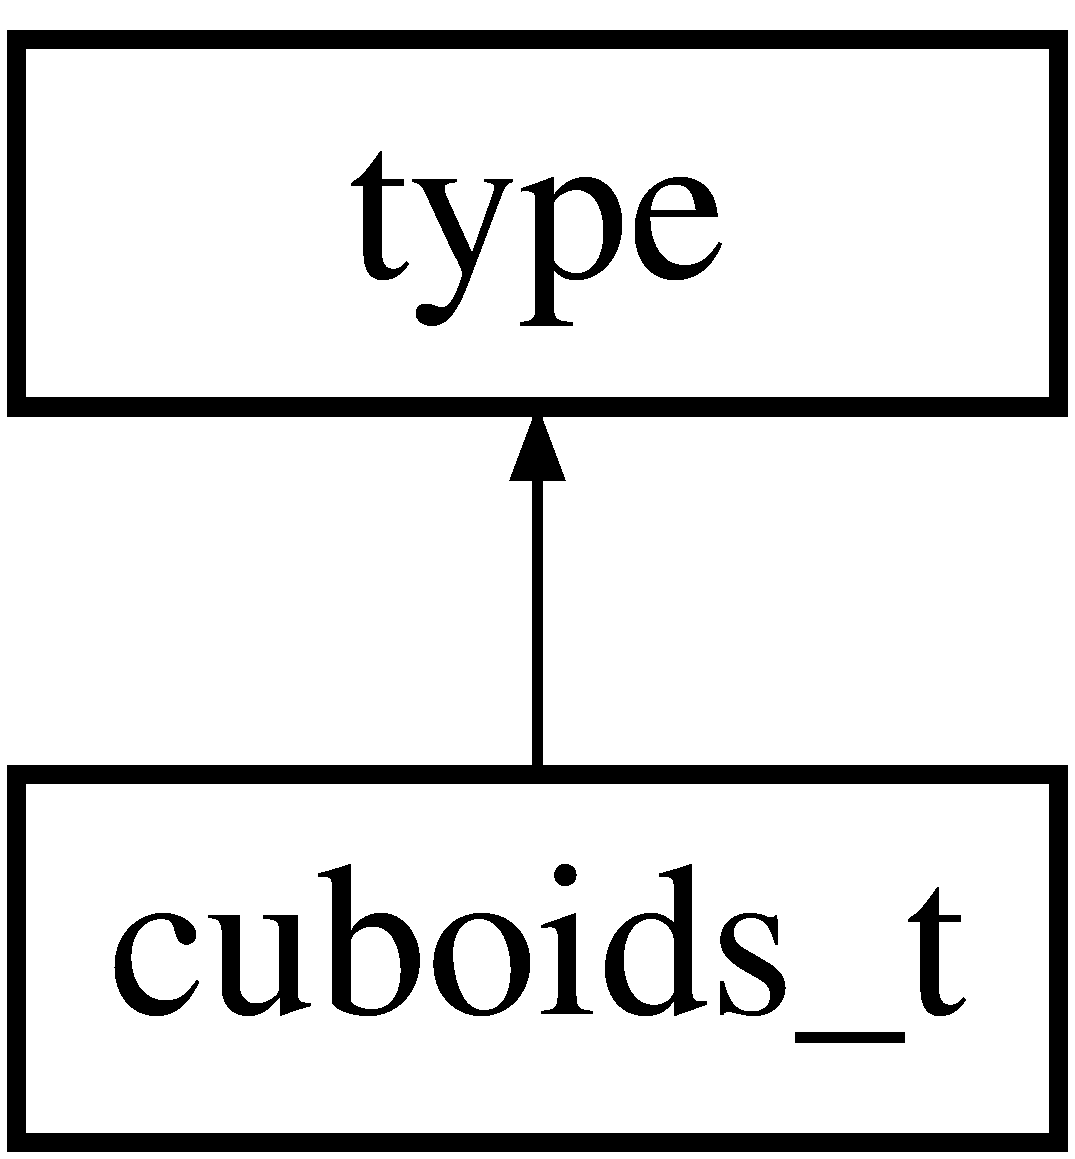
\includegraphics[height=2.000000cm]{classcuboids__t}
\end{center}
\end{figure}
\subsection*{Public Types}
\begin{DoxyCompactItemize}
\item 
typedef \-::\hyperlink{classcuboid__t}{cuboid\-\_\-t} \hyperlink{classcuboids__t_a7c920a1afd759302a5672d5ba2eb9707}{cuboid\-\_\-type}
\item 
typedef \\*
\-::xsd\-::cxx\-::tree\-::sequence\\*
$<$ \hyperlink{classcuboids__t_a7c920a1afd759302a5672d5ba2eb9707}{cuboid\-\_\-type} $>$ \hyperlink{classcuboids__t_ae3d3abd50bb0570dfe0d4d2d97485261}{cuboid\-\_\-sequence}
\item 
typedef cuboid\-\_\-sequence\-::iterator \hyperlink{classcuboids__t_a63fead1ce5b1d5d61e641a72d80349e9}{cuboid\-\_\-iterator}
\item 
typedef \\*
cuboid\-\_\-sequence\-::const\-\_\-iterator \hyperlink{classcuboids__t_a4c6feaefcda62b64615c74892b835b04}{cuboid\-\_\-const\-\_\-iterator}
\item 
typedef \\*
\-::xsd\-::cxx\-::tree\-::traits\\*
$<$ \hyperlink{classcuboids__t_a7c920a1afd759302a5672d5ba2eb9707}{cuboid\-\_\-type}, char $>$ \hyperlink{classcuboids__t_a070c3f6592d095cd861a6e1f31271ae2}{cuboid\-\_\-traits}
\end{DoxyCompactItemize}
\subsection*{Public Member Functions}
\begin{DoxyCompactItemize}
\item 
const \hyperlink{classcuboids__t_ae3d3abd50bb0570dfe0d4d2d97485261}{cuboid\-\_\-sequence} \& \hyperlink{classcuboids__t_aeb1e3d9339c27438d0b05fa28836a164}{cuboid} () const 
\item 
\hyperlink{classcuboids__t_ae3d3abd50bb0570dfe0d4d2d97485261}{cuboid\-\_\-sequence} \& \hyperlink{classcuboids__t_a91312ccc2a7af492294fa940c5b92302}{cuboid} ()
\item 
void \hyperlink{classcuboids__t_ab05aa257894ab2b0fddf4b40fab766e3}{cuboid} (const \hyperlink{classcuboids__t_ae3d3abd50bb0570dfe0d4d2d97485261}{cuboid\-\_\-sequence} \&s)
\item 
\hyperlink{classcuboids__t_a56be77bec0772d60210b3f79ecd7517a}{cuboids\-\_\-t} ()
\item 
\hyperlink{classcuboids__t_ab8bb7bb7d61bcbb5a7c424c1a352b97a}{cuboids\-\_\-t} (const \-::xercesc\-::\-D\-O\-M\-Element \&e,\-::\hyperlink{namespacexml__schema_a0612287d030cb2732d31a45b258fdc87}{xml\-\_\-schema\-::flags} f=0,\-::\hyperlink{namespacexml__schema_ada9aa30dc722e93ee2ed7243085402a5}{xml\-\_\-schema\-::container} $\ast$c=0)
\item 
\hyperlink{classcuboids__t_a47833a6b8a1a427de79a8efa8ba86dc0}{cuboids\-\_\-t} (const \hyperlink{classcuboids__t}{cuboids\-\_\-t} \&x,\-::\hyperlink{namespacexml__schema_a0612287d030cb2732d31a45b258fdc87}{xml\-\_\-schema\-::flags} f=0,\-::\hyperlink{namespacexml__schema_ada9aa30dc722e93ee2ed7243085402a5}{xml\-\_\-schema\-::container} $\ast$c=0)
\item 
virtual \hyperlink{classcuboids__t}{cuboids\-\_\-t} $\ast$ \hyperlink{classcuboids__t_a4dae998f9ea7ba9a2321d49d2f617f87}{\-\_\-clone} (\-::\hyperlink{namespacexml__schema_a0612287d030cb2732d31a45b258fdc87}{xml\-\_\-schema\-::flags} f=0,\-::\hyperlink{namespacexml__schema_ada9aa30dc722e93ee2ed7243085402a5}{xml\-\_\-schema\-::container} $\ast$c=0) const 
\item 
virtual \hyperlink{classcuboids__t_a8dcfc7aab5951518c3c28e7a0db699ee}{$\sim$cuboids\-\_\-t} ()
\end{DoxyCompactItemize}
\subsection*{Protected Member Functions}
\begin{DoxyCompactItemize}
\item 
void \hyperlink{classcuboids__t_a63261d4cd5babc19315baa9db3db4cbb}{parse} (\-::xsd\-::cxx\-::xml\-::dom\-::parser$<$ char $>$ \&,\-::\hyperlink{namespacexml__schema_a0612287d030cb2732d31a45b258fdc87}{xml\-\_\-schema\-::flags})
\end{DoxyCompactItemize}
\subsection*{Protected Attributes}
\begin{DoxyCompactItemize}
\item 
\hyperlink{classcuboids__t_ae3d3abd50bb0570dfe0d4d2d97485261}{cuboid\-\_\-sequence} \hyperlink{classcuboids__t_a82604cb9beb9bfd3620947e4729e167e}{cuboid\-\_\-}
\end{DoxyCompactItemize}


\subsection{Member Typedef Documentation}
\hypertarget{classcuboids__t_a4c6feaefcda62b64615c74892b835b04}{\index{cuboids\-\_\-t@{cuboids\-\_\-t}!cuboid\-\_\-const\-\_\-iterator@{cuboid\-\_\-const\-\_\-iterator}}
\index{cuboid\-\_\-const\-\_\-iterator@{cuboid\-\_\-const\-\_\-iterator}!cuboids_t@{cuboids\-\_\-t}}
\subsubsection[{cuboid\-\_\-const\-\_\-iterator}]{\setlength{\rightskip}{0pt plus 5cm}typedef cuboid\-\_\-sequence\-::const\-\_\-iterator {\bf cuboids\-\_\-t\-::cuboid\-\_\-const\-\_\-iterator}}}\label{classcuboids__t_a4c6feaefcda62b64615c74892b835b04}
\hypertarget{classcuboids__t_a63fead1ce5b1d5d61e641a72d80349e9}{\index{cuboids\-\_\-t@{cuboids\-\_\-t}!cuboid\-\_\-iterator@{cuboid\-\_\-iterator}}
\index{cuboid\-\_\-iterator@{cuboid\-\_\-iterator}!cuboids_t@{cuboids\-\_\-t}}
\subsubsection[{cuboid\-\_\-iterator}]{\setlength{\rightskip}{0pt plus 5cm}typedef cuboid\-\_\-sequence\-::iterator {\bf cuboids\-\_\-t\-::cuboid\-\_\-iterator}}}\label{classcuboids__t_a63fead1ce5b1d5d61e641a72d80349e9}
\hypertarget{classcuboids__t_ae3d3abd50bb0570dfe0d4d2d97485261}{\index{cuboids\-\_\-t@{cuboids\-\_\-t}!cuboid\-\_\-sequence@{cuboid\-\_\-sequence}}
\index{cuboid\-\_\-sequence@{cuboid\-\_\-sequence}!cuboids_t@{cuboids\-\_\-t}}
\subsubsection[{cuboid\-\_\-sequence}]{\setlength{\rightskip}{0pt plus 5cm}typedef \-::xsd\-::cxx\-::tree\-::sequence$<$ {\bf cuboid\-\_\-type} $>$ {\bf cuboids\-\_\-t\-::cuboid\-\_\-sequence}}}\label{classcuboids__t_ae3d3abd50bb0570dfe0d4d2d97485261}
\hypertarget{classcuboids__t_a070c3f6592d095cd861a6e1f31271ae2}{\index{cuboids\-\_\-t@{cuboids\-\_\-t}!cuboid\-\_\-traits@{cuboid\-\_\-traits}}
\index{cuboid\-\_\-traits@{cuboid\-\_\-traits}!cuboids_t@{cuboids\-\_\-t}}
\subsubsection[{cuboid\-\_\-traits}]{\setlength{\rightskip}{0pt plus 5cm}typedef \-::xsd\-::cxx\-::tree\-::traits$<$ {\bf cuboid\-\_\-type}, char $>$ {\bf cuboids\-\_\-t\-::cuboid\-\_\-traits}}}\label{classcuboids__t_a070c3f6592d095cd861a6e1f31271ae2}
\hypertarget{classcuboids__t_a7c920a1afd759302a5672d5ba2eb9707}{\index{cuboids\-\_\-t@{cuboids\-\_\-t}!cuboid\-\_\-type@{cuboid\-\_\-type}}
\index{cuboid\-\_\-type@{cuboid\-\_\-type}!cuboids_t@{cuboids\-\_\-t}}
\subsubsection[{cuboid\-\_\-type}]{\setlength{\rightskip}{0pt plus 5cm}typedef \-::{\bf cuboid\-\_\-t} {\bf cuboids\-\_\-t\-::cuboid\-\_\-type}}}\label{classcuboids__t_a7c920a1afd759302a5672d5ba2eb9707}


\subsection{Constructor \& Destructor Documentation}
\hypertarget{classcuboids__t_a56be77bec0772d60210b3f79ecd7517a}{\index{cuboids\-\_\-t@{cuboids\-\_\-t}!cuboids\-\_\-t@{cuboids\-\_\-t}}
\index{cuboids\-\_\-t@{cuboids\-\_\-t}!cuboids_t@{cuboids\-\_\-t}}
\subsubsection[{cuboids\-\_\-t}]{\setlength{\rightskip}{0pt plus 5cm}cuboids\-\_\-t\-::cuboids\-\_\-t (
\begin{DoxyParamCaption}
{}
\end{DoxyParamCaption}
)}}\label{classcuboids__t_a56be77bec0772d60210b3f79ecd7517a}
\hypertarget{classcuboids__t_ab8bb7bb7d61bcbb5a7c424c1a352b97a}{\index{cuboids\-\_\-t@{cuboids\-\_\-t}!cuboids\-\_\-t@{cuboids\-\_\-t}}
\index{cuboids\-\_\-t@{cuboids\-\_\-t}!cuboids_t@{cuboids\-\_\-t}}
\subsubsection[{cuboids\-\_\-t}]{\setlength{\rightskip}{0pt plus 5cm}cuboids\-\_\-t\-::cuboids\-\_\-t (
\begin{DoxyParamCaption}
\item[{const \-::xercesc\-::\-D\-O\-M\-Element \&}]{e, }
\item[{\-::{\bf xml\-\_\-schema\-::flags}}]{f = {\ttfamily 0}, }
\item[{\-::{\bf xml\-\_\-schema\-::container} $\ast$}]{c = {\ttfamily 0}}
\end{DoxyParamCaption}
)}}\label{classcuboids__t_ab8bb7bb7d61bcbb5a7c424c1a352b97a}
\hypertarget{classcuboids__t_a47833a6b8a1a427de79a8efa8ba86dc0}{\index{cuboids\-\_\-t@{cuboids\-\_\-t}!cuboids\-\_\-t@{cuboids\-\_\-t}}
\index{cuboids\-\_\-t@{cuboids\-\_\-t}!cuboids_t@{cuboids\-\_\-t}}
\subsubsection[{cuboids\-\_\-t}]{\setlength{\rightskip}{0pt plus 5cm}cuboids\-\_\-t\-::cuboids\-\_\-t (
\begin{DoxyParamCaption}
\item[{const {\bf cuboids\-\_\-t} \&}]{x, }
\item[{\-::{\bf xml\-\_\-schema\-::flags}}]{f = {\ttfamily 0}, }
\item[{\-::{\bf xml\-\_\-schema\-::container} $\ast$}]{c = {\ttfamily 0}}
\end{DoxyParamCaption}
)}}\label{classcuboids__t_a47833a6b8a1a427de79a8efa8ba86dc0}
\hypertarget{classcuboids__t_a8dcfc7aab5951518c3c28e7a0db699ee}{\index{cuboids\-\_\-t@{cuboids\-\_\-t}!$\sim$cuboids\-\_\-t@{$\sim$cuboids\-\_\-t}}
\index{$\sim$cuboids\-\_\-t@{$\sim$cuboids\-\_\-t}!cuboids_t@{cuboids\-\_\-t}}
\subsubsection[{$\sim$cuboids\-\_\-t}]{\setlength{\rightskip}{0pt plus 5cm}cuboids\-\_\-t\-::$\sim$cuboids\-\_\-t (
\begin{DoxyParamCaption}
{}
\end{DoxyParamCaption}
)\hspace{0.3cm}{\ttfamily [virtual]}}}\label{classcuboids__t_a8dcfc7aab5951518c3c28e7a0db699ee}


\subsection{Member Function Documentation}
\hypertarget{classcuboids__t_a4dae998f9ea7ba9a2321d49d2f617f87}{\index{cuboids\-\_\-t@{cuboids\-\_\-t}!\-\_\-clone@{\-\_\-clone}}
\index{\-\_\-clone@{\-\_\-clone}!cuboids_t@{cuboids\-\_\-t}}
\subsubsection[{\-\_\-clone}]{\setlength{\rightskip}{0pt plus 5cm}{\bf cuboids\-\_\-t} $\ast$ cuboids\-\_\-t\-::\-\_\-clone (
\begin{DoxyParamCaption}
\item[{\-::{\bf xml\-\_\-schema\-::flags}}]{f = {\ttfamily 0}, }
\item[{\-::{\bf xml\-\_\-schema\-::container} $\ast$}]{c = {\ttfamily 0}}
\end{DoxyParamCaption}
) const\hspace{0.3cm}{\ttfamily [virtual]}}}\label{classcuboids__t_a4dae998f9ea7ba9a2321d49d2f617f87}
\hypertarget{classcuboids__t_aeb1e3d9339c27438d0b05fa28836a164}{\index{cuboids\-\_\-t@{cuboids\-\_\-t}!cuboid@{cuboid}}
\index{cuboid@{cuboid}!cuboids_t@{cuboids\-\_\-t}}
\subsubsection[{cuboid}]{\setlength{\rightskip}{0pt plus 5cm}const {\bf cuboids\-\_\-t\-::cuboid\-\_\-sequence} \& cuboids\-\_\-t\-::cuboid (
\begin{DoxyParamCaption}
{}
\end{DoxyParamCaption}
) const}}\label{classcuboids__t_aeb1e3d9339c27438d0b05fa28836a164}
\hypertarget{classcuboids__t_a91312ccc2a7af492294fa940c5b92302}{\index{cuboids\-\_\-t@{cuboids\-\_\-t}!cuboid@{cuboid}}
\index{cuboid@{cuboid}!cuboids_t@{cuboids\-\_\-t}}
\subsubsection[{cuboid}]{\setlength{\rightskip}{0pt plus 5cm}{\bf cuboids\-\_\-t\-::cuboid\-\_\-sequence} \& cuboids\-\_\-t\-::cuboid (
\begin{DoxyParamCaption}
{}
\end{DoxyParamCaption}
)}}\label{classcuboids__t_a91312ccc2a7af492294fa940c5b92302}
\hypertarget{classcuboids__t_ab05aa257894ab2b0fddf4b40fab766e3}{\index{cuboids\-\_\-t@{cuboids\-\_\-t}!cuboid@{cuboid}}
\index{cuboid@{cuboid}!cuboids_t@{cuboids\-\_\-t}}
\subsubsection[{cuboid}]{\setlength{\rightskip}{0pt plus 5cm}void cuboids\-\_\-t\-::cuboid (
\begin{DoxyParamCaption}
\item[{const {\bf cuboid\-\_\-sequence} \&}]{s}
\end{DoxyParamCaption}
)}}\label{classcuboids__t_ab05aa257894ab2b0fddf4b40fab766e3}
\hypertarget{classcuboids__t_a63261d4cd5babc19315baa9db3db4cbb}{\index{cuboids\-\_\-t@{cuboids\-\_\-t}!parse@{parse}}
\index{parse@{parse}!cuboids_t@{cuboids\-\_\-t}}
\subsubsection[{parse}]{\setlength{\rightskip}{0pt plus 5cm}void cuboids\-\_\-t\-::parse (
\begin{DoxyParamCaption}
\item[{\-::xsd\-::cxx\-::xml\-::dom\-::parser$<$ char $>$ \&}]{p, }
\item[{\-::{\bf xml\-\_\-schema\-::flags}}]{f}
\end{DoxyParamCaption}
)\hspace{0.3cm}{\ttfamily [protected]}}}\label{classcuboids__t_a63261d4cd5babc19315baa9db3db4cbb}


\subsection{Member Data Documentation}
\hypertarget{classcuboids__t_a82604cb9beb9bfd3620947e4729e167e}{\index{cuboids\-\_\-t@{cuboids\-\_\-t}!cuboid\-\_\-@{cuboid\-\_\-}}
\index{cuboid\-\_\-@{cuboid\-\_\-}!cuboids_t@{cuboids\-\_\-t}}
\subsubsection[{cuboid\-\_\-}]{\setlength{\rightskip}{0pt plus 5cm}{\bf cuboid\-\_\-sequence} cuboids\-\_\-t\-::cuboid\-\_\-\hspace{0.3cm}{\ttfamily [protected]}}}\label{classcuboids__t_a82604cb9beb9bfd3620947e4729e167e}


The documentation for this class was generated from the following files\-:\begin{DoxyCompactItemize}
\item 
src/utils/\hyperlink{InputCuboids_8h}{Input\-Cuboids.\-h}\item 
src/utils/\hyperlink{InputCuboids_8cpp}{Input\-Cuboids.\-cpp}\end{DoxyCompactItemize}

\hypertarget{classDataArray__t}{\section{Data\-Array\-\_\-t Class Reference}
\label{classDataArray__t}\index{Data\-Array\-\_\-t@{Data\-Array\-\_\-t}}
}


Class corresponding to the Data\-Array\-\_\-t schema type.  




{\ttfamily \#include $<$vtk-\/unstructured.\-h$>$}

Inheritance diagram for Data\-Array\-\_\-t\-:\begin{figure}[H]
\begin{center}
\leavevmode
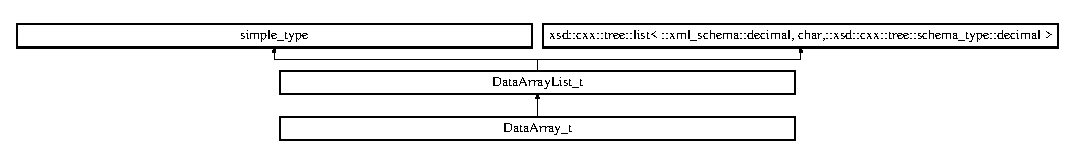
\includegraphics[height=1.660079cm]{classDataArray__t}
\end{center}
\end{figure}
\subsection*{Public Member Functions}
\begin{DoxyCompactItemize}
\item 
virtual \hyperlink{classDataArray__t_ac9806a5eedf7abecd7adf6408c8af894}{$\sim$\-Data\-Array\-\_\-t} ()
\begin{DoxyCompactList}\small\item\em Destructor. \end{DoxyCompactList}\end{DoxyCompactItemize}
\subsection*{type}
\label{_amgrp599dcce2998a6b40b1e38e8c6006cb0a}%
Accessor and modifier functions for the type required attribute. \begin{DoxyCompactItemize}
\item 
typedef \-::\hyperlink{classtype}{type} \hyperlink{classDataArray__t_a484a0509e4f141d9970d75881703a51e}{type\-\_\-type}
\begin{DoxyCompactList}\small\item\em Attribute type. \end{DoxyCompactList}\item 
typedef \\*
\-::xsd\-::cxx\-::tree\-::traits\\*
$<$ \hyperlink{classDataArray__t_a484a0509e4f141d9970d75881703a51e}{type\-\_\-type}, char $>$ \hyperlink{classDataArray__t_af1dc5f097a8645ae42b57eb3a0b10fa2}{type\-\_\-traits}
\begin{DoxyCompactList}\small\item\em Attribute traits type. \end{DoxyCompactList}\item 
const \hyperlink{classDataArray__t_a484a0509e4f141d9970d75881703a51e}{type\-\_\-type} \& \hyperlink{classDataArray__t_a6ec3c246d1a2fddc7052bcde2cb6bdf7}{type} () const 
\begin{DoxyCompactList}\small\item\em Return a read-\/only (constant) reference to the attribute. \end{DoxyCompactList}\item 
\hyperlink{classDataArray__t_a484a0509e4f141d9970d75881703a51e}{type\-\_\-type} \& \hyperlink{classDataArray__t_a29f3ed42a5bf8df9437ece5f63c02301}{type} ()
\begin{DoxyCompactList}\small\item\em Return a read-\/write reference to the attribute. \end{DoxyCompactList}\item 
void \hyperlink{classDataArray__t_ae4fd6c47e992055ec42cc1949b60da2a}{type} (const \hyperlink{classDataArray__t_a484a0509e4f141d9970d75881703a51e}{type\-\_\-type} \&x)
\begin{DoxyCompactList}\small\item\em Set the attribute value. \end{DoxyCompactList}\item 
void \hyperlink{classDataArray__t_afa90d226889ba3e7baa5c8e9dba594d2}{type} (\-::std\-::auto\-\_\-ptr$<$ \hyperlink{classDataArray__t_a484a0509e4f141d9970d75881703a51e}{type\-\_\-type} $>$ p)
\begin{DoxyCompactList}\small\item\em Set the attribute value without copying. \end{DoxyCompactList}\end{DoxyCompactItemize}
\subsection*{Name}
\label{_amgrp49ee3087348e8d44e1feda1917443987}%
Accessor and modifier functions for the Name required attribute. \begin{DoxyCompactItemize}
\item 
typedef \-::\hyperlink{namespacexml__schema_ac0cec83a330f0024e4e318b3deac5104}{xml\-\_\-schema\-::string} \hyperlink{classDataArray__t_afc6836923916c2489f91caea78ec4ad6}{Name\-\_\-type}
\begin{DoxyCompactList}\small\item\em Attribute type. \end{DoxyCompactList}\item 
typedef \\*
\-::xsd\-::cxx\-::tree\-::traits\\*
$<$ \hyperlink{classDataArray__t_afc6836923916c2489f91caea78ec4ad6}{Name\-\_\-type}, char $>$ \hyperlink{classDataArray__t_a46d0b4cf44ee9122e4cbb3bd3abe6663}{Name\-\_\-traits}
\begin{DoxyCompactList}\small\item\em Attribute traits type. \end{DoxyCompactList}\item 
const \hyperlink{classDataArray__t_afc6836923916c2489f91caea78ec4ad6}{Name\-\_\-type} \& \hyperlink{classDataArray__t_ada03ebff820f73d64d0761a0fb977527}{Name} () const 
\begin{DoxyCompactList}\small\item\em Return a read-\/only (constant) reference to the attribute. \end{DoxyCompactList}\item 
\hyperlink{classDataArray__t_afc6836923916c2489f91caea78ec4ad6}{Name\-\_\-type} \& \hyperlink{classDataArray__t_aeb126f8a8b03eea44eed5a2b606da59c}{Name} ()
\begin{DoxyCompactList}\small\item\em Return a read-\/write reference to the attribute. \end{DoxyCompactList}\item 
void \hyperlink{classDataArray__t_a95a1f49a6dd9f54fb71fb6b70240a51b}{Name} (const \hyperlink{classDataArray__t_afc6836923916c2489f91caea78ec4ad6}{Name\-\_\-type} \&x)
\begin{DoxyCompactList}\small\item\em Set the attribute value. \end{DoxyCompactList}\item 
void \hyperlink{classDataArray__t_a290f1b5702b7a623a0c9fc086a7a0d0c}{Name} (\-::std\-::auto\-\_\-ptr$<$ \hyperlink{classDataArray__t_afc6836923916c2489f91caea78ec4ad6}{Name\-\_\-type} $>$ p)
\begin{DoxyCompactList}\small\item\em Set the attribute value without copying. \end{DoxyCompactList}\end{DoxyCompactItemize}
\subsection*{Number\-Of\-Components}
\label{_amgrp2a0e258c3f78050b74e96bb0ed643748}%
Accessor and modifier functions for the Number\-Of\-Components required attribute. \begin{DoxyCompactItemize}
\item 
typedef \-::\hyperlink{namespacexml__schema_aaaea7c8ce4dfbe26cc52c91c29c97b7c}{xml\-\_\-schema\-::integer} \hyperlink{classDataArray__t_aac602cec132f6e771f7fa3be1d19c16f}{Number\-Of\-Components\-\_\-type}
\begin{DoxyCompactList}\small\item\em Attribute type. \end{DoxyCompactList}\item 
typedef \\*
\-::xsd\-::cxx\-::tree\-::traits\\*
$<$ \hyperlink{classDataArray__t_aac602cec132f6e771f7fa3be1d19c16f}{Number\-Of\-Components\-\_\-type}, \\*
char $>$ \hyperlink{classDataArray__t_a1112148f87db2c0ba05323377d9f0427}{Number\-Of\-Components\-\_\-traits}
\begin{DoxyCompactList}\small\item\em Attribute traits type. \end{DoxyCompactList}\item 
const \hyperlink{classDataArray__t_aac602cec132f6e771f7fa3be1d19c16f}{Number\-Of\-Components\-\_\-type} \& \hyperlink{classDataArray__t_a715a5b58a694d49499591bfea3a282ae}{Number\-Of\-Components} () const 
\begin{DoxyCompactList}\small\item\em Return a read-\/only (constant) reference to the attribute. \end{DoxyCompactList}\item 
\hyperlink{classDataArray__t_aac602cec132f6e771f7fa3be1d19c16f}{Number\-Of\-Components\-\_\-type} \& \hyperlink{classDataArray__t_a6f80fc5ce05d51d4292c698464d4ace3}{Number\-Of\-Components} ()
\begin{DoxyCompactList}\small\item\em Return a read-\/write reference to the attribute. \end{DoxyCompactList}\item 
void \hyperlink{classDataArray__t_a755fae9b31318f98a3d21beba16f2841}{Number\-Of\-Components} (const \hyperlink{classDataArray__t_aac602cec132f6e771f7fa3be1d19c16f}{Number\-Of\-Components\-\_\-type} \&x)
\begin{DoxyCompactList}\small\item\em Set the attribute value. \end{DoxyCompactList}\end{DoxyCompactItemize}
\subsection*{format}
\label{_amgrp1ddcb92ade31c8fbd370001f9b29a7d9}%
Accessor and modifier functions for the format optional attribute with a default value. \begin{DoxyCompactItemize}
\item 
typedef \-::\hyperlink{namespacexml__schema_ac0cec83a330f0024e4e318b3deac5104}{xml\-\_\-schema\-::string} \hyperlink{classDataArray__t_ae453ea653980baef2e3296005d70bfbd}{format\-\_\-type}
\begin{DoxyCompactList}\small\item\em Attribute type. \end{DoxyCompactList}\item 
typedef \\*
\-::xsd\-::cxx\-::tree\-::traits\\*
$<$ \hyperlink{classDataArray__t_ae453ea653980baef2e3296005d70bfbd}{format\-\_\-type}, char $>$ \hyperlink{classDataArray__t_a2a31ef3ce1dfa973843a02e17762e7a3}{format\-\_\-traits}
\begin{DoxyCompactList}\small\item\em Attribute traits type. \end{DoxyCompactList}\item 
const \hyperlink{classDataArray__t_ae453ea653980baef2e3296005d70bfbd}{format\-\_\-type} \& \hyperlink{classDataArray__t_a7a39cab4205282736e633d8a3c57bbae}{format} () const 
\begin{DoxyCompactList}\small\item\em Return a read-\/only (constant) reference to the attribute. \end{DoxyCompactList}\item 
static const \hyperlink{classDataArray__t_ae453ea653980baef2e3296005d70bfbd}{format\-\_\-type} \& \hyperlink{classDataArray__t_ade99ea2c2fdc45cc2826b6847dfb5404}{format\-\_\-default\-\_\-value} ()
\begin{DoxyCompactList}\small\item\em Return the default value for the attribute. \end{DoxyCompactList}\end{DoxyCompactItemize}
\subsection*{offset}
\label{_amgrp7a86c157ee9713c34fbd7a1ee40f0c5a}%
Accessor and modifier functions for the offset optional attribute. \begin{DoxyCompactItemize}
\item 
typedef \-::\hyperlink{namespacexml__schema_aaaea7c8ce4dfbe26cc52c91c29c97b7c}{xml\-\_\-schema\-::integer} \hyperlink{classDataArray__t_a7b840c5f08bd2c65cd3c5e24ad132cfb}{offset\-\_\-type}
\begin{DoxyCompactList}\small\item\em Attribute type. \end{DoxyCompactList}\item 
typedef \\*
\-::xsd\-::cxx\-::tree\-::optional\\*
$<$ \hyperlink{classDataArray__t_a7b840c5f08bd2c65cd3c5e24ad132cfb}{offset\-\_\-type} $>$ \hyperlink{classDataArray__t_a4bc33060e7c386b658c752347ac5f03e}{offset\-\_\-optional}
\begin{DoxyCompactList}\small\item\em Attribute optional container type. \end{DoxyCompactList}\item 
typedef \\*
\-::xsd\-::cxx\-::tree\-::traits\\*
$<$ \hyperlink{classDataArray__t_a7b840c5f08bd2c65cd3c5e24ad132cfb}{offset\-\_\-type}, char $>$ \hyperlink{classDataArray__t_a2e3e1a5de665fc64a3d86fd94bb1af0f}{offset\-\_\-traits}
\begin{DoxyCompactList}\small\item\em Attribute traits type. \end{DoxyCompactList}\item 
const \hyperlink{classDataArray__t_a4bc33060e7c386b658c752347ac5f03e}{offset\-\_\-optional} \& \hyperlink{classDataArray__t_a995d24c5c7a88929a6b0e7de154bbdf5}{offset} () const 
\begin{DoxyCompactList}\small\item\em Return a read-\/only (constant) reference to the attribute container. \end{DoxyCompactList}\item 
\hyperlink{classDataArray__t_a4bc33060e7c386b658c752347ac5f03e}{offset\-\_\-optional} \& \hyperlink{classDataArray__t_aed72cbf5f3476360f4898f487a074c26}{offset} ()
\begin{DoxyCompactList}\small\item\em Return a read-\/write reference to the attribute container. \end{DoxyCompactList}\item 
void \hyperlink{classDataArray__t_ac133def4ed8ae6c623d0144f036a18d7}{offset} (const \hyperlink{classDataArray__t_a7b840c5f08bd2c65cd3c5e24ad132cfb}{offset\-\_\-type} \&x)
\begin{DoxyCompactList}\small\item\em Set the attribute value. \end{DoxyCompactList}\item 
void \hyperlink{classDataArray__t_a5abb95d7ab6fb95015c06de57a6ccbc9}{offset} (const \hyperlink{classDataArray__t_a4bc33060e7c386b658c752347ac5f03e}{offset\-\_\-optional} \&x)
\begin{DoxyCompactList}\small\item\em Set the attribute value. \end{DoxyCompactList}\end{DoxyCompactItemize}
\subsection*{Constructors}
\begin{DoxyCompactItemize}
\item 
\hyperlink{classDataArray__t_a0700e9e63538064c2f9eb668fe3ca624}{Data\-Array\-\_\-t} (const \hyperlink{classDataArray__t_a484a0509e4f141d9970d75881703a51e}{type\-\_\-type} \&, const \hyperlink{classDataArray__t_afc6836923916c2489f91caea78ec4ad6}{Name\-\_\-type} \&, const \hyperlink{classDataArray__t_aac602cec132f6e771f7fa3be1d19c16f}{Number\-Of\-Components\-\_\-type} \&)
\begin{DoxyCompactList}\small\item\em Create an instance from initializers for required elements and attributes. \end{DoxyCompactList}\item 
\hyperlink{classDataArray__t_a3c07c46f9c607ce6da2d2e456494465a}{Data\-Array\-\_\-t} (const \-::\hyperlink{classDataArrayList__t}{Data\-Array\-List\-\_\-t} \&, const \hyperlink{classDataArray__t_a484a0509e4f141d9970d75881703a51e}{type\-\_\-type} \&, const \hyperlink{classDataArray__t_afc6836923916c2489f91caea78ec4ad6}{Name\-\_\-type} \&, const \hyperlink{classDataArray__t_aac602cec132f6e771f7fa3be1d19c16f}{Number\-Of\-Components\-\_\-type} \&)
\begin{DoxyCompactList}\small\item\em Create an instance from the ultimate base and initializers for required elements and attributes. \end{DoxyCompactList}\item 
\hyperlink{classDataArray__t_ae02d07853318c1d754e0acfc80f5c894}{Data\-Array\-\_\-t} (const \-::xercesc\-::\-D\-O\-M\-Element \&e,\-::\hyperlink{namespacexml__schema_a0612287d030cb2732d31a45b258fdc87}{xml\-\_\-schema\-::flags} f=0,\-::\hyperlink{namespacexml__schema_ada9aa30dc722e93ee2ed7243085402a5}{xml\-\_\-schema\-::container} $\ast$c=0)
\begin{DoxyCompactList}\small\item\em Create an instance from a D\-O\-M element. \end{DoxyCompactList}\item 
\hyperlink{classDataArray__t_a6f67fee4225ca87492d8496de4121de7}{Data\-Array\-\_\-t} (const \hyperlink{classDataArray__t}{Data\-Array\-\_\-t} \&x,\-::\hyperlink{namespacexml__schema_a0612287d030cb2732d31a45b258fdc87}{xml\-\_\-schema\-::flags} f=0,\-::\hyperlink{namespacexml__schema_ada9aa30dc722e93ee2ed7243085402a5}{xml\-\_\-schema\-::container} $\ast$c=0)
\begin{DoxyCompactList}\small\item\em Copy constructor. \end{DoxyCompactList}\item 
virtual \hyperlink{classDataArray__t}{Data\-Array\-\_\-t} $\ast$ \hyperlink{classDataArray__t_a0ba3569846912b9fcadbd942e914cce1}{\-\_\-clone} (\-::\hyperlink{namespacexml__schema_a0612287d030cb2732d31a45b258fdc87}{xml\-\_\-schema\-::flags} f=0,\-::\hyperlink{namespacexml__schema_ada9aa30dc722e93ee2ed7243085402a5}{xml\-\_\-schema\-::container} $\ast$c=0) const 
\begin{DoxyCompactList}\small\item\em Copy the instance polymorphically. \end{DoxyCompactList}\end{DoxyCompactItemize}


\subsection{Detailed Description}
Class corresponding to the Data\-Array\-\_\-t schema type. 

\subsection{Member Typedef Documentation}
\hypertarget{classDataArray__t_a2a31ef3ce1dfa973843a02e17762e7a3}{\index{Data\-Array\-\_\-t@{Data\-Array\-\_\-t}!format\-\_\-traits@{format\-\_\-traits}}
\index{format\-\_\-traits@{format\-\_\-traits}!DataArray_t@{Data\-Array\-\_\-t}}
\subsubsection[{format\-\_\-traits}]{\setlength{\rightskip}{0pt plus 5cm}typedef \-::xsd\-::cxx\-::tree\-::traits$<$ {\bf format\-\_\-type}, char $>$ {\bf Data\-Array\-\_\-t\-::format\-\_\-traits}}}\label{classDataArray__t_a2a31ef3ce1dfa973843a02e17762e7a3}


Attribute traits type. 

\hypertarget{classDataArray__t_ae453ea653980baef2e3296005d70bfbd}{\index{Data\-Array\-\_\-t@{Data\-Array\-\_\-t}!format\-\_\-type@{format\-\_\-type}}
\index{format\-\_\-type@{format\-\_\-type}!DataArray_t@{Data\-Array\-\_\-t}}
\subsubsection[{format\-\_\-type}]{\setlength{\rightskip}{0pt plus 5cm}typedef \-::{\bf xml\-\_\-schema\-::string} {\bf Data\-Array\-\_\-t\-::format\-\_\-type}}}\label{classDataArray__t_ae453ea653980baef2e3296005d70bfbd}


Attribute type. 

\hypertarget{classDataArray__t_a46d0b4cf44ee9122e4cbb3bd3abe6663}{\index{Data\-Array\-\_\-t@{Data\-Array\-\_\-t}!Name\-\_\-traits@{Name\-\_\-traits}}
\index{Name\-\_\-traits@{Name\-\_\-traits}!DataArray_t@{Data\-Array\-\_\-t}}
\subsubsection[{Name\-\_\-traits}]{\setlength{\rightskip}{0pt plus 5cm}typedef \-::xsd\-::cxx\-::tree\-::traits$<$ {\bf Name\-\_\-type}, char $>$ {\bf Data\-Array\-\_\-t\-::\-Name\-\_\-traits}}}\label{classDataArray__t_a46d0b4cf44ee9122e4cbb3bd3abe6663}


Attribute traits type. 

\hypertarget{classDataArray__t_afc6836923916c2489f91caea78ec4ad6}{\index{Data\-Array\-\_\-t@{Data\-Array\-\_\-t}!Name\-\_\-type@{Name\-\_\-type}}
\index{Name\-\_\-type@{Name\-\_\-type}!DataArray_t@{Data\-Array\-\_\-t}}
\subsubsection[{Name\-\_\-type}]{\setlength{\rightskip}{0pt plus 5cm}typedef \-::{\bf xml\-\_\-schema\-::string} {\bf Data\-Array\-\_\-t\-::\-Name\-\_\-type}}}\label{classDataArray__t_afc6836923916c2489f91caea78ec4ad6}


Attribute type. 

\hypertarget{classDataArray__t_a1112148f87db2c0ba05323377d9f0427}{\index{Data\-Array\-\_\-t@{Data\-Array\-\_\-t}!Number\-Of\-Components\-\_\-traits@{Number\-Of\-Components\-\_\-traits}}
\index{Number\-Of\-Components\-\_\-traits@{Number\-Of\-Components\-\_\-traits}!DataArray_t@{Data\-Array\-\_\-t}}
\subsubsection[{Number\-Of\-Components\-\_\-traits}]{\setlength{\rightskip}{0pt plus 5cm}typedef \-::xsd\-::cxx\-::tree\-::traits$<$ {\bf Number\-Of\-Components\-\_\-type}, char $>$ {\bf Data\-Array\-\_\-t\-::\-Number\-Of\-Components\-\_\-traits}}}\label{classDataArray__t_a1112148f87db2c0ba05323377d9f0427}


Attribute traits type. 

\hypertarget{classDataArray__t_aac602cec132f6e771f7fa3be1d19c16f}{\index{Data\-Array\-\_\-t@{Data\-Array\-\_\-t}!Number\-Of\-Components\-\_\-type@{Number\-Of\-Components\-\_\-type}}
\index{Number\-Of\-Components\-\_\-type@{Number\-Of\-Components\-\_\-type}!DataArray_t@{Data\-Array\-\_\-t}}
\subsubsection[{Number\-Of\-Components\-\_\-type}]{\setlength{\rightskip}{0pt plus 5cm}typedef \-::{\bf xml\-\_\-schema\-::integer} {\bf Data\-Array\-\_\-t\-::\-Number\-Of\-Components\-\_\-type}}}\label{classDataArray__t_aac602cec132f6e771f7fa3be1d19c16f}


Attribute type. 

\hypertarget{classDataArray__t_a4bc33060e7c386b658c752347ac5f03e}{\index{Data\-Array\-\_\-t@{Data\-Array\-\_\-t}!offset\-\_\-optional@{offset\-\_\-optional}}
\index{offset\-\_\-optional@{offset\-\_\-optional}!DataArray_t@{Data\-Array\-\_\-t}}
\subsubsection[{offset\-\_\-optional}]{\setlength{\rightskip}{0pt plus 5cm}typedef \-::xsd\-::cxx\-::tree\-::optional$<$ {\bf offset\-\_\-type} $>$ {\bf Data\-Array\-\_\-t\-::offset\-\_\-optional}}}\label{classDataArray__t_a4bc33060e7c386b658c752347ac5f03e}


Attribute optional container type. 

\hypertarget{classDataArray__t_a2e3e1a5de665fc64a3d86fd94bb1af0f}{\index{Data\-Array\-\_\-t@{Data\-Array\-\_\-t}!offset\-\_\-traits@{offset\-\_\-traits}}
\index{offset\-\_\-traits@{offset\-\_\-traits}!DataArray_t@{Data\-Array\-\_\-t}}
\subsubsection[{offset\-\_\-traits}]{\setlength{\rightskip}{0pt plus 5cm}typedef \-::xsd\-::cxx\-::tree\-::traits$<$ {\bf offset\-\_\-type}, char $>$ {\bf Data\-Array\-\_\-t\-::offset\-\_\-traits}}}\label{classDataArray__t_a2e3e1a5de665fc64a3d86fd94bb1af0f}


Attribute traits type. 

\hypertarget{classDataArray__t_a7b840c5f08bd2c65cd3c5e24ad132cfb}{\index{Data\-Array\-\_\-t@{Data\-Array\-\_\-t}!offset\-\_\-type@{offset\-\_\-type}}
\index{offset\-\_\-type@{offset\-\_\-type}!DataArray_t@{Data\-Array\-\_\-t}}
\subsubsection[{offset\-\_\-type}]{\setlength{\rightskip}{0pt plus 5cm}typedef \-::{\bf xml\-\_\-schema\-::integer} {\bf Data\-Array\-\_\-t\-::offset\-\_\-type}}}\label{classDataArray__t_a7b840c5f08bd2c65cd3c5e24ad132cfb}


Attribute type. 

\hypertarget{classDataArray__t_af1dc5f097a8645ae42b57eb3a0b10fa2}{\index{Data\-Array\-\_\-t@{Data\-Array\-\_\-t}!type\-\_\-traits@{type\-\_\-traits}}
\index{type\-\_\-traits@{type\-\_\-traits}!DataArray_t@{Data\-Array\-\_\-t}}
\subsubsection[{type\-\_\-traits}]{\setlength{\rightskip}{0pt plus 5cm}typedef \-::xsd\-::cxx\-::tree\-::traits$<$ {\bf type\-\_\-type}, char $>$ {\bf Data\-Array\-\_\-t\-::type\-\_\-traits}}}\label{classDataArray__t_af1dc5f097a8645ae42b57eb3a0b10fa2}


Attribute traits type. 

\hypertarget{classDataArray__t_a484a0509e4f141d9970d75881703a51e}{\index{Data\-Array\-\_\-t@{Data\-Array\-\_\-t}!type\-\_\-type@{type\-\_\-type}}
\index{type\-\_\-type@{type\-\_\-type}!DataArray_t@{Data\-Array\-\_\-t}}
\subsubsection[{type\-\_\-type}]{\setlength{\rightskip}{0pt plus 5cm}typedef \-::{\bf type} {\bf Data\-Array\-\_\-t\-::type\-\_\-type}}}\label{classDataArray__t_a484a0509e4f141d9970d75881703a51e}


Attribute type. 



\subsection{Constructor \& Destructor Documentation}
\hypertarget{classDataArray__t_a0700e9e63538064c2f9eb668fe3ca624}{\index{Data\-Array\-\_\-t@{Data\-Array\-\_\-t}!Data\-Array\-\_\-t@{Data\-Array\-\_\-t}}
\index{Data\-Array\-\_\-t@{Data\-Array\-\_\-t}!DataArray_t@{Data\-Array\-\_\-t}}
\subsubsection[{Data\-Array\-\_\-t}]{\setlength{\rightskip}{0pt plus 5cm}Data\-Array\-\_\-t\-::\-Data\-Array\-\_\-t (
\begin{DoxyParamCaption}
\item[{const {\bf type\-\_\-type} \&}]{type, }
\item[{const {\bf Name\-\_\-type} \&}]{Name, }
\item[{const {\bf Number\-Of\-Components\-\_\-type} \&}]{Number\-Of\-Components}
\end{DoxyParamCaption}
)}}\label{classDataArray__t_a0700e9e63538064c2f9eb668fe3ca624}


Create an instance from initializers for required elements and attributes. 

\hypertarget{classDataArray__t_a3c07c46f9c607ce6da2d2e456494465a}{\index{Data\-Array\-\_\-t@{Data\-Array\-\_\-t}!Data\-Array\-\_\-t@{Data\-Array\-\_\-t}}
\index{Data\-Array\-\_\-t@{Data\-Array\-\_\-t}!DataArray_t@{Data\-Array\-\_\-t}}
\subsubsection[{Data\-Array\-\_\-t}]{\setlength{\rightskip}{0pt plus 5cm}Data\-Array\-\_\-t\-::\-Data\-Array\-\_\-t (
\begin{DoxyParamCaption}
\item[{const \-::{\bf Data\-Array\-List\-\_\-t} \&}]{\-\_\-xsd\-\_\-\-Data\-Array\-List\-\_\-t\-\_\-base, }
\item[{const {\bf type\-\_\-type} \&}]{type, }
\item[{const {\bf Name\-\_\-type} \&}]{Name, }
\item[{const {\bf Number\-Of\-Components\-\_\-type} \&}]{Number\-Of\-Components}
\end{DoxyParamCaption}
)}}\label{classDataArray__t_a3c07c46f9c607ce6da2d2e456494465a}


Create an instance from the ultimate base and initializers for required elements and attributes. 

\hypertarget{classDataArray__t_ae02d07853318c1d754e0acfc80f5c894}{\index{Data\-Array\-\_\-t@{Data\-Array\-\_\-t}!Data\-Array\-\_\-t@{Data\-Array\-\_\-t}}
\index{Data\-Array\-\_\-t@{Data\-Array\-\_\-t}!DataArray_t@{Data\-Array\-\_\-t}}
\subsubsection[{Data\-Array\-\_\-t}]{\setlength{\rightskip}{0pt plus 5cm}Data\-Array\-\_\-t\-::\-Data\-Array\-\_\-t (
\begin{DoxyParamCaption}
\item[{const \-::xercesc\-::\-D\-O\-M\-Element \&}]{e, }
\item[{\-::{\bf xml\-\_\-schema\-::flags}}]{f = {\ttfamily 0}, }
\item[{\-::{\bf xml\-\_\-schema\-::container} $\ast$}]{c = {\ttfamily 0}}
\end{DoxyParamCaption}
)}}\label{classDataArray__t_ae02d07853318c1d754e0acfc80f5c894}


Create an instance from a D\-O\-M element. 


\begin{DoxyParams}{Parameters}
{\em e} & A D\-O\-M element to extract the data from. \\
\hline
{\em f} & Flags to create the new instance with. \\
\hline
{\em c} & A pointer to the object that will contain the new instance. \\
\hline
\end{DoxyParams}
\hypertarget{classDataArray__t_a6f67fee4225ca87492d8496de4121de7}{\index{Data\-Array\-\_\-t@{Data\-Array\-\_\-t}!Data\-Array\-\_\-t@{Data\-Array\-\_\-t}}
\index{Data\-Array\-\_\-t@{Data\-Array\-\_\-t}!DataArray_t@{Data\-Array\-\_\-t}}
\subsubsection[{Data\-Array\-\_\-t}]{\setlength{\rightskip}{0pt plus 5cm}Data\-Array\-\_\-t\-::\-Data\-Array\-\_\-t (
\begin{DoxyParamCaption}
\item[{const {\bf Data\-Array\-\_\-t} \&}]{x, }
\item[{\-::{\bf xml\-\_\-schema\-::flags}}]{f = {\ttfamily 0}, }
\item[{\-::{\bf xml\-\_\-schema\-::container} $\ast$}]{c = {\ttfamily 0}}
\end{DoxyParamCaption}
)}}\label{classDataArray__t_a6f67fee4225ca87492d8496de4121de7}


Copy constructor. 


\begin{DoxyParams}{Parameters}
{\em x} & An instance to make a copy of. \\
\hline
{\em f} & Flags to create the copy with. \\
\hline
{\em c} & A pointer to the object that will contain the copy.\\
\hline
\end{DoxyParams}
For polymorphic object models use the {\ttfamily \-\_\-clone} function instead. \hypertarget{classDataArray__t_ac9806a5eedf7abecd7adf6408c8af894}{\index{Data\-Array\-\_\-t@{Data\-Array\-\_\-t}!$\sim$\-Data\-Array\-\_\-t@{$\sim$\-Data\-Array\-\_\-t}}
\index{$\sim$\-Data\-Array\-\_\-t@{$\sim$\-Data\-Array\-\_\-t}!DataArray_t@{Data\-Array\-\_\-t}}
\subsubsection[{$\sim$\-Data\-Array\-\_\-t}]{\setlength{\rightskip}{0pt plus 5cm}Data\-Array\-\_\-t\-::$\sim$\-Data\-Array\-\_\-t (
\begin{DoxyParamCaption}
{}
\end{DoxyParamCaption}
)\hspace{0.3cm}{\ttfamily [virtual]}}}\label{classDataArray__t_ac9806a5eedf7abecd7adf6408c8af894}


Destructor. 



\subsection{Member Function Documentation}
\hypertarget{classDataArray__t_a0ba3569846912b9fcadbd942e914cce1}{\index{Data\-Array\-\_\-t@{Data\-Array\-\_\-t}!\-\_\-clone@{\-\_\-clone}}
\index{\-\_\-clone@{\-\_\-clone}!DataArray_t@{Data\-Array\-\_\-t}}
\subsubsection[{\-\_\-clone}]{\setlength{\rightskip}{0pt plus 5cm}{\bf Data\-Array\-\_\-t} $\ast$ Data\-Array\-\_\-t\-::\-\_\-clone (
\begin{DoxyParamCaption}
\item[{\-::{\bf xml\-\_\-schema\-::flags}}]{f = {\ttfamily 0}, }
\item[{\-::{\bf xml\-\_\-schema\-::container} $\ast$}]{c = {\ttfamily 0}}
\end{DoxyParamCaption}
) const\hspace{0.3cm}{\ttfamily [virtual]}}}\label{classDataArray__t_a0ba3569846912b9fcadbd942e914cce1}


Copy the instance polymorphically. 


\begin{DoxyParams}{Parameters}
{\em f} & Flags to create the copy with. \\
\hline
{\em c} & A pointer to the object that will contain the copy. \\
\hline
\end{DoxyParams}
\begin{DoxyReturn}{Returns}
A pointer to the dynamically allocated copy.
\end{DoxyReturn}
This function ensures that the dynamic type of the instance is used for copying and should be used for polymorphic object models instead of the copy constructor. 

Reimplemented from \hyperlink{classDataArrayList__t_acec29e88488ded1352c5b064827f5c38}{Data\-Array\-List\-\_\-t}.

\hypertarget{classDataArray__t_a7a39cab4205282736e633d8a3c57bbae}{\index{Data\-Array\-\_\-t@{Data\-Array\-\_\-t}!format@{format}}
\index{format@{format}!DataArray_t@{Data\-Array\-\_\-t}}
\subsubsection[{format}]{\setlength{\rightskip}{0pt plus 5cm}const {\bf Data\-Array\-\_\-t\-::format\-\_\-type} \& Data\-Array\-\_\-t\-::format (
\begin{DoxyParamCaption}
{}
\end{DoxyParamCaption}
) const}}\label{classDataArray__t_a7a39cab4205282736e633d8a3c57bbae}


Return a read-\/only (constant) reference to the attribute. 

\begin{DoxyReturn}{Returns}
A constant reference to the attribute. 
\end{DoxyReturn}
\hypertarget{classDataArray__t_ade99ea2c2fdc45cc2826b6847dfb5404}{\index{Data\-Array\-\_\-t@{Data\-Array\-\_\-t}!format\-\_\-default\-\_\-value@{format\-\_\-default\-\_\-value}}
\index{format\-\_\-default\-\_\-value@{format\-\_\-default\-\_\-value}!DataArray_t@{Data\-Array\-\_\-t}}
\subsubsection[{format\-\_\-default\-\_\-value}]{\setlength{\rightskip}{0pt plus 5cm}const {\bf Data\-Array\-\_\-t\-::format\-\_\-type} \& Data\-Array\-\_\-t\-::format\-\_\-default\-\_\-value (
\begin{DoxyParamCaption}
{}
\end{DoxyParamCaption}
)\hspace{0.3cm}{\ttfamily [static]}}}\label{classDataArray__t_ade99ea2c2fdc45cc2826b6847dfb5404}


Return the default value for the attribute. 

\begin{DoxyReturn}{Returns}
A read-\/only (constant) reference to the attribute's default value. 
\end{DoxyReturn}
\hypertarget{classDataArray__t_ada03ebff820f73d64d0761a0fb977527}{\index{Data\-Array\-\_\-t@{Data\-Array\-\_\-t}!Name@{Name}}
\index{Name@{Name}!DataArray_t@{Data\-Array\-\_\-t}}
\subsubsection[{Name}]{\setlength{\rightskip}{0pt plus 5cm}const {\bf Data\-Array\-\_\-t\-::\-Name\-\_\-type} \& Data\-Array\-\_\-t\-::\-Name (
\begin{DoxyParamCaption}
{}
\end{DoxyParamCaption}
) const}}\label{classDataArray__t_ada03ebff820f73d64d0761a0fb977527}


Return a read-\/only (constant) reference to the attribute. 

\begin{DoxyReturn}{Returns}
A constant reference to the attribute. 
\end{DoxyReturn}
\hypertarget{classDataArray__t_aeb126f8a8b03eea44eed5a2b606da59c}{\index{Data\-Array\-\_\-t@{Data\-Array\-\_\-t}!Name@{Name}}
\index{Name@{Name}!DataArray_t@{Data\-Array\-\_\-t}}
\subsubsection[{Name}]{\setlength{\rightskip}{0pt plus 5cm}{\bf Data\-Array\-\_\-t\-::\-Name\-\_\-type} \& Data\-Array\-\_\-t\-::\-Name (
\begin{DoxyParamCaption}
{}
\end{DoxyParamCaption}
)}}\label{classDataArray__t_aeb126f8a8b03eea44eed5a2b606da59c}


Return a read-\/write reference to the attribute. 

\begin{DoxyReturn}{Returns}
A reference to the attribute. 
\end{DoxyReturn}
\hypertarget{classDataArray__t_a95a1f49a6dd9f54fb71fb6b70240a51b}{\index{Data\-Array\-\_\-t@{Data\-Array\-\_\-t}!Name@{Name}}
\index{Name@{Name}!DataArray_t@{Data\-Array\-\_\-t}}
\subsubsection[{Name}]{\setlength{\rightskip}{0pt plus 5cm}void Data\-Array\-\_\-t\-::\-Name (
\begin{DoxyParamCaption}
\item[{const {\bf Name\-\_\-type} \&}]{x}
\end{DoxyParamCaption}
)}}\label{classDataArray__t_a95a1f49a6dd9f54fb71fb6b70240a51b}


Set the attribute value. 


\begin{DoxyParams}{Parameters}
{\em x} & A new value to set.\\
\hline
\end{DoxyParams}
This function makes a copy of its argument and sets it as the new value of the attribute. \hypertarget{classDataArray__t_a290f1b5702b7a623a0c9fc086a7a0d0c}{\index{Data\-Array\-\_\-t@{Data\-Array\-\_\-t}!Name@{Name}}
\index{Name@{Name}!DataArray_t@{Data\-Array\-\_\-t}}
\subsubsection[{Name}]{\setlength{\rightskip}{0pt plus 5cm}void Data\-Array\-\_\-t\-::\-Name (
\begin{DoxyParamCaption}
\item[{\-::std\-::auto\-\_\-ptr$<$ {\bf Name\-\_\-type} $>$}]{p}
\end{DoxyParamCaption}
)}}\label{classDataArray__t_a290f1b5702b7a623a0c9fc086a7a0d0c}


Set the attribute value without copying. 


\begin{DoxyParams}{Parameters}
{\em p} & A new value to use.\\
\hline
\end{DoxyParams}
This function will try to use the passed value directly instead of making a copy. \hypertarget{classDataArray__t_a715a5b58a694d49499591bfea3a282ae}{\index{Data\-Array\-\_\-t@{Data\-Array\-\_\-t}!Number\-Of\-Components@{Number\-Of\-Components}}
\index{Number\-Of\-Components@{Number\-Of\-Components}!DataArray_t@{Data\-Array\-\_\-t}}
\subsubsection[{Number\-Of\-Components}]{\setlength{\rightskip}{0pt plus 5cm}const {\bf Data\-Array\-\_\-t\-::\-Number\-Of\-Components\-\_\-type} \& Data\-Array\-\_\-t\-::\-Number\-Of\-Components (
\begin{DoxyParamCaption}
{}
\end{DoxyParamCaption}
) const}}\label{classDataArray__t_a715a5b58a694d49499591bfea3a282ae}


Return a read-\/only (constant) reference to the attribute. 

\begin{DoxyReturn}{Returns}
A constant reference to the attribute. 
\end{DoxyReturn}
\hypertarget{classDataArray__t_a6f80fc5ce05d51d4292c698464d4ace3}{\index{Data\-Array\-\_\-t@{Data\-Array\-\_\-t}!Number\-Of\-Components@{Number\-Of\-Components}}
\index{Number\-Of\-Components@{Number\-Of\-Components}!DataArray_t@{Data\-Array\-\_\-t}}
\subsubsection[{Number\-Of\-Components}]{\setlength{\rightskip}{0pt plus 5cm}{\bf Data\-Array\-\_\-t\-::\-Number\-Of\-Components\-\_\-type} \& Data\-Array\-\_\-t\-::\-Number\-Of\-Components (
\begin{DoxyParamCaption}
{}
\end{DoxyParamCaption}
)}}\label{classDataArray__t_a6f80fc5ce05d51d4292c698464d4ace3}


Return a read-\/write reference to the attribute. 

\begin{DoxyReturn}{Returns}
A reference to the attribute. 
\end{DoxyReturn}
\hypertarget{classDataArray__t_a755fae9b31318f98a3d21beba16f2841}{\index{Data\-Array\-\_\-t@{Data\-Array\-\_\-t}!Number\-Of\-Components@{Number\-Of\-Components}}
\index{Number\-Of\-Components@{Number\-Of\-Components}!DataArray_t@{Data\-Array\-\_\-t}}
\subsubsection[{Number\-Of\-Components}]{\setlength{\rightskip}{0pt plus 5cm}void Data\-Array\-\_\-t\-::\-Number\-Of\-Components (
\begin{DoxyParamCaption}
\item[{const {\bf Number\-Of\-Components\-\_\-type} \&}]{x}
\end{DoxyParamCaption}
)}}\label{classDataArray__t_a755fae9b31318f98a3d21beba16f2841}


Set the attribute value. 


\begin{DoxyParams}{Parameters}
{\em x} & A new value to set.\\
\hline
\end{DoxyParams}
This function makes a copy of its argument and sets it as the new value of the attribute. \hypertarget{classDataArray__t_a995d24c5c7a88929a6b0e7de154bbdf5}{\index{Data\-Array\-\_\-t@{Data\-Array\-\_\-t}!offset@{offset}}
\index{offset@{offset}!DataArray_t@{Data\-Array\-\_\-t}}
\subsubsection[{offset}]{\setlength{\rightskip}{0pt plus 5cm}const {\bf Data\-Array\-\_\-t\-::offset\-\_\-optional} \& Data\-Array\-\_\-t\-::offset (
\begin{DoxyParamCaption}
{}
\end{DoxyParamCaption}
) const}}\label{classDataArray__t_a995d24c5c7a88929a6b0e7de154bbdf5}


Return a read-\/only (constant) reference to the attribute container. 

\begin{DoxyReturn}{Returns}
A constant reference to the optional container. 
\end{DoxyReturn}
\hypertarget{classDataArray__t_aed72cbf5f3476360f4898f487a074c26}{\index{Data\-Array\-\_\-t@{Data\-Array\-\_\-t}!offset@{offset}}
\index{offset@{offset}!DataArray_t@{Data\-Array\-\_\-t}}
\subsubsection[{offset}]{\setlength{\rightskip}{0pt plus 5cm}{\bf Data\-Array\-\_\-t\-::offset\-\_\-optional} \& Data\-Array\-\_\-t\-::offset (
\begin{DoxyParamCaption}
{}
\end{DoxyParamCaption}
)}}\label{classDataArray__t_aed72cbf5f3476360f4898f487a074c26}


Return a read-\/write reference to the attribute container. 

\begin{DoxyReturn}{Returns}
A reference to the optional container. 
\end{DoxyReturn}
\hypertarget{classDataArray__t_ac133def4ed8ae6c623d0144f036a18d7}{\index{Data\-Array\-\_\-t@{Data\-Array\-\_\-t}!offset@{offset}}
\index{offset@{offset}!DataArray_t@{Data\-Array\-\_\-t}}
\subsubsection[{offset}]{\setlength{\rightskip}{0pt plus 5cm}void Data\-Array\-\_\-t\-::offset (
\begin{DoxyParamCaption}
\item[{const {\bf offset\-\_\-type} \&}]{x}
\end{DoxyParamCaption}
)}}\label{classDataArray__t_ac133def4ed8ae6c623d0144f036a18d7}


Set the attribute value. 


\begin{DoxyParams}{Parameters}
{\em x} & A new value to set.\\
\hline
\end{DoxyParams}
This function makes a copy of its argument and sets it as the new value of the attribute. \hypertarget{classDataArray__t_a5abb95d7ab6fb95015c06de57a6ccbc9}{\index{Data\-Array\-\_\-t@{Data\-Array\-\_\-t}!offset@{offset}}
\index{offset@{offset}!DataArray_t@{Data\-Array\-\_\-t}}
\subsubsection[{offset}]{\setlength{\rightskip}{0pt plus 5cm}void Data\-Array\-\_\-t\-::offset (
\begin{DoxyParamCaption}
\item[{const {\bf offset\-\_\-optional} \&}]{x}
\end{DoxyParamCaption}
)}}\label{classDataArray__t_a5abb95d7ab6fb95015c06de57a6ccbc9}


Set the attribute value. 


\begin{DoxyParams}{Parameters}
{\em x} & An optional container with the new value to set.\\
\hline
\end{DoxyParams}
If the value is present in {\itshape x} then this function makes a copy of this value and sets it as the new value of the attribute. Otherwise the attribute container is set the 'not present' state. \hypertarget{classDataArray__t_a6ec3c246d1a2fddc7052bcde2cb6bdf7}{\index{Data\-Array\-\_\-t@{Data\-Array\-\_\-t}!type@{type}}
\index{type@{type}!DataArray_t@{Data\-Array\-\_\-t}}
\subsubsection[{type}]{\setlength{\rightskip}{0pt plus 5cm}const {\bf Data\-Array\-\_\-t\-::type\-\_\-type} \& Data\-Array\-\_\-t\-::type (
\begin{DoxyParamCaption}
{}
\end{DoxyParamCaption}
) const}}\label{classDataArray__t_a6ec3c246d1a2fddc7052bcde2cb6bdf7}


Return a read-\/only (constant) reference to the attribute. 

\begin{DoxyReturn}{Returns}
A constant reference to the attribute. 
\end{DoxyReturn}
\hypertarget{classDataArray__t_a29f3ed42a5bf8df9437ece5f63c02301}{\index{Data\-Array\-\_\-t@{Data\-Array\-\_\-t}!type@{type}}
\index{type@{type}!DataArray_t@{Data\-Array\-\_\-t}}
\subsubsection[{type}]{\setlength{\rightskip}{0pt plus 5cm}{\bf Data\-Array\-\_\-t\-::type\-\_\-type} \& Data\-Array\-\_\-t\-::type (
\begin{DoxyParamCaption}
{}
\end{DoxyParamCaption}
)}}\label{classDataArray__t_a29f3ed42a5bf8df9437ece5f63c02301}


Return a read-\/write reference to the attribute. 

\begin{DoxyReturn}{Returns}
A reference to the attribute. 
\end{DoxyReturn}
\hypertarget{classDataArray__t_ae4fd6c47e992055ec42cc1949b60da2a}{\index{Data\-Array\-\_\-t@{Data\-Array\-\_\-t}!type@{type}}
\index{type@{type}!DataArray_t@{Data\-Array\-\_\-t}}
\subsubsection[{type}]{\setlength{\rightskip}{0pt plus 5cm}void Data\-Array\-\_\-t\-::type (
\begin{DoxyParamCaption}
\item[{const {\bf type\-\_\-type} \&}]{x}
\end{DoxyParamCaption}
)}}\label{classDataArray__t_ae4fd6c47e992055ec42cc1949b60da2a}


Set the attribute value. 


\begin{DoxyParams}{Parameters}
{\em x} & A new value to set.\\
\hline
\end{DoxyParams}
This function makes a copy of its argument and sets it as the new value of the attribute. \hypertarget{classDataArray__t_afa90d226889ba3e7baa5c8e9dba594d2}{\index{Data\-Array\-\_\-t@{Data\-Array\-\_\-t}!type@{type}}
\index{type@{type}!DataArray_t@{Data\-Array\-\_\-t}}
\subsubsection[{type}]{\setlength{\rightskip}{0pt plus 5cm}void Data\-Array\-\_\-t\-::type (
\begin{DoxyParamCaption}
\item[{\-::std\-::auto\-\_\-ptr$<$ {\bf type\-\_\-type} $>$}]{p}
\end{DoxyParamCaption}
)}}\label{classDataArray__t_afa90d226889ba3e7baa5c8e9dba594d2}


Set the attribute value without copying. 


\begin{DoxyParams}{Parameters}
{\em p} & A new value to use.\\
\hline
\end{DoxyParams}
This function will try to use the passed value directly instead of making a copy. 

The documentation for this class was generated from the following files\-:\begin{DoxyCompactItemize}
\item 
src/output\-Writer/\hyperlink{vtk-unstructured_8h}{vtk-\/unstructured.\-h}\item 
src/output\-Writer/\hyperlink{vtk-unstructured_8cpp}{vtk-\/unstructured.\-cpp}\end{DoxyCompactItemize}

\hypertarget{classDataArrayList__t}{\section{Data\-Array\-List\-\_\-t Class Reference}
\label{classDataArrayList__t}\index{Data\-Array\-List\-\_\-t@{Data\-Array\-List\-\_\-t}}
}


List class corresponding to the Data\-Array\-List\-\_\-t schema type.  




{\ttfamily \#include $<$vtk-\/unstructured.\-h$>$}

Inheritance diagram for Data\-Array\-List\-\_\-t\-:\begin{figure}[H]
\begin{center}
\leavevmode
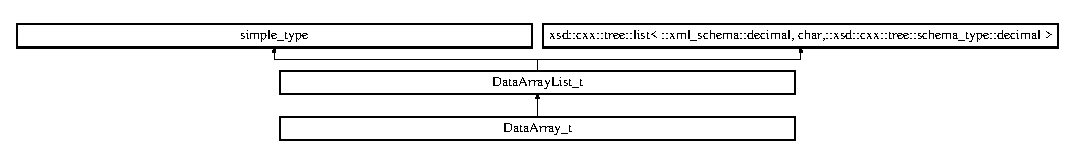
\includegraphics[height=1.660079cm]{classDataArrayList__t}
\end{center}
\end{figure}
\subsection*{Public Member Functions}
\begin{DoxyCompactItemize}
\item 
\hyperlink{classDataArrayList__t_a3ec10a5824450940e47a90c376fdb065}{Data\-Array\-List\-\_\-t} ()
\begin{DoxyCompactList}\small\item\em Default constructor. \end{DoxyCompactList}\item 
\hyperlink{classDataArrayList__t_ad821001ed5f5f94f06712f5b0acab874}{Data\-Array\-List\-\_\-t} (size\-\_\-type n, const \-::\hyperlink{namespacexml__schema_a69bfaf24f63a8c18ebd8e21db6b343df}{xml\-\_\-schema\-::decimal} \&x)
\begin{DoxyCompactList}\small\item\em Create a list with copies of the specified element. \end{DoxyCompactList}\item 
{\footnotesize template$<$typename I $>$ }\\\hyperlink{classDataArrayList__t_a7b3c40bcc5d41bafc235a30ffa1a3b8f}{Data\-Array\-List\-\_\-t} (const I \&begin, const I \&end)
\begin{DoxyCompactList}\small\item\em Create a list from an iterator range. \end{DoxyCompactList}\item 
\hyperlink{classDataArrayList__t_ab596ca97e9666c979d1db13a4e032869}{Data\-Array\-List\-\_\-t} (const \-::xercesc\-::\-D\-O\-M\-Element \&e,\-::\hyperlink{namespacexml__schema_a0612287d030cb2732d31a45b258fdc87}{xml\-\_\-schema\-::flags} f=0,\-::\hyperlink{namespacexml__schema_ada9aa30dc722e93ee2ed7243085402a5}{xml\-\_\-schema\-::container} $\ast$c=0)
\begin{DoxyCompactList}\small\item\em Create an instance from a D\-O\-M element. \end{DoxyCompactList}\item 
\hyperlink{classDataArrayList__t_a4cae1891a3ad2b9336b478fa436f4d3f}{Data\-Array\-List\-\_\-t} (const \-::xercesc\-::\-D\-O\-M\-Attr \&a,\-::\hyperlink{namespacexml__schema_a0612287d030cb2732d31a45b258fdc87}{xml\-\_\-schema\-::flags} f=0,\-::\hyperlink{namespacexml__schema_ada9aa30dc722e93ee2ed7243085402a5}{xml\-\_\-schema\-::container} $\ast$c=0)
\begin{DoxyCompactList}\small\item\em Create an instance from a D\-O\-M attribute. \end{DoxyCompactList}\item 
\hyperlink{classDataArrayList__t_a360a3281299fcb02ad34ad0b2c2d15fd}{Data\-Array\-List\-\_\-t} (const \-::std\-::string \&s, const \-::xercesc\-::\-D\-O\-M\-Element $\ast$e,\-::\hyperlink{namespacexml__schema_a0612287d030cb2732d31a45b258fdc87}{xml\-\_\-schema\-::flags} f=0,\-::\hyperlink{namespacexml__schema_ada9aa30dc722e93ee2ed7243085402a5}{xml\-\_\-schema\-::container} $\ast$c=0)
\begin{DoxyCompactList}\small\item\em Create an instance from a string fragment. \end{DoxyCompactList}\item 
\hyperlink{classDataArrayList__t_af44b66e9ba5c6f84a3a0cca1c0fc98dc}{Data\-Array\-List\-\_\-t} (const \hyperlink{classDataArrayList__t}{Data\-Array\-List\-\_\-t} \&x,\-::\hyperlink{namespacexml__schema_a0612287d030cb2732d31a45b258fdc87}{xml\-\_\-schema\-::flags} f=0,\-::\hyperlink{namespacexml__schema_ada9aa30dc722e93ee2ed7243085402a5}{xml\-\_\-schema\-::container} $\ast$c=0)
\begin{DoxyCompactList}\small\item\em Copy constructor. \end{DoxyCompactList}\item 
virtual \hyperlink{classDataArrayList__t}{Data\-Array\-List\-\_\-t} $\ast$ \hyperlink{classDataArrayList__t_acec29e88488ded1352c5b064827f5c38}{\-\_\-clone} (\-::\hyperlink{namespacexml__schema_a0612287d030cb2732d31a45b258fdc87}{xml\-\_\-schema\-::flags} f=0,\-::\hyperlink{namespacexml__schema_ada9aa30dc722e93ee2ed7243085402a5}{xml\-\_\-schema\-::container} $\ast$c=0) const 
\begin{DoxyCompactList}\small\item\em Copy the instance polymorphically. \end{DoxyCompactList}\item 
virtual \hyperlink{classDataArrayList__t_aee3c16237122c72a9c163847232d830f}{$\sim$\-Data\-Array\-List\-\_\-t} ()
\begin{DoxyCompactList}\small\item\em Destructor. \end{DoxyCompactList}\end{DoxyCompactItemize}


\subsection{Detailed Description}
List class corresponding to the Data\-Array\-List\-\_\-t schema type. 

This class has an interface of a standard C++ sequence (e.\-g., std\-::vector). 

\subsection{Constructor \& Destructor Documentation}
\hypertarget{classDataArrayList__t_a3ec10a5824450940e47a90c376fdb065}{\index{Data\-Array\-List\-\_\-t@{Data\-Array\-List\-\_\-t}!Data\-Array\-List\-\_\-t@{Data\-Array\-List\-\_\-t}}
\index{Data\-Array\-List\-\_\-t@{Data\-Array\-List\-\_\-t}!DataArrayList_t@{Data\-Array\-List\-\_\-t}}
\subsubsection[{Data\-Array\-List\-\_\-t}]{\setlength{\rightskip}{0pt plus 5cm}Data\-Array\-List\-\_\-t\-::\-Data\-Array\-List\-\_\-t (
\begin{DoxyParamCaption}
{}
\end{DoxyParamCaption}
)}}\label{classDataArrayList__t_a3ec10a5824450940e47a90c376fdb065}


Default constructor. 

Creates an empty list. \hypertarget{classDataArrayList__t_ad821001ed5f5f94f06712f5b0acab874}{\index{Data\-Array\-List\-\_\-t@{Data\-Array\-List\-\_\-t}!Data\-Array\-List\-\_\-t@{Data\-Array\-List\-\_\-t}}
\index{Data\-Array\-List\-\_\-t@{Data\-Array\-List\-\_\-t}!DataArrayList_t@{Data\-Array\-List\-\_\-t}}
\subsubsection[{Data\-Array\-List\-\_\-t}]{\setlength{\rightskip}{0pt plus 5cm}Data\-Array\-List\-\_\-t\-::\-Data\-Array\-List\-\_\-t (
\begin{DoxyParamCaption}
\item[{size\-\_\-type}]{n, }
\item[{const \-::{\bf xml\-\_\-schema\-::decimal} \&}]{x}
\end{DoxyParamCaption}
)}}\label{classDataArrayList__t_ad821001ed5f5f94f06712f5b0acab874}


Create a list with copies of the specified element. 


\begin{DoxyParams}{Parameters}
{\em n} & A number of elements to copy. \\
\hline
{\em x} & An element to copy.\\
\hline
\end{DoxyParams}
This constructor creates a list with {\itshape n} copies of {\itshape x}. \hypertarget{classDataArrayList__t_a7b3c40bcc5d41bafc235a30ffa1a3b8f}{\index{Data\-Array\-List\-\_\-t@{Data\-Array\-List\-\_\-t}!Data\-Array\-List\-\_\-t@{Data\-Array\-List\-\_\-t}}
\index{Data\-Array\-List\-\_\-t@{Data\-Array\-List\-\_\-t}!DataArrayList_t@{Data\-Array\-List\-\_\-t}}
\subsubsection[{Data\-Array\-List\-\_\-t}]{\setlength{\rightskip}{0pt plus 5cm}template$<$typename I $>$ Data\-Array\-List\-\_\-t\-::\-Data\-Array\-List\-\_\-t (
\begin{DoxyParamCaption}
\item[{const I \&}]{begin, }
\item[{const I \&}]{end}
\end{DoxyParamCaption}
)\hspace{0.3cm}{\ttfamily [inline]}}}\label{classDataArrayList__t_a7b3c40bcc5d41bafc235a30ffa1a3b8f}


Create a list from an iterator range. 


\begin{DoxyParams}{Parameters}
{\em begin} & An iterator pointing to the first element. \\
\hline
{\em end} & An iterator pointing to the one past the last element.\\
\hline
\end{DoxyParams}
This constructor creates a list consisting of copies of the elements in the range \mbox{[}begin,end). \hypertarget{classDataArrayList__t_ab596ca97e9666c979d1db13a4e032869}{\index{Data\-Array\-List\-\_\-t@{Data\-Array\-List\-\_\-t}!Data\-Array\-List\-\_\-t@{Data\-Array\-List\-\_\-t}}
\index{Data\-Array\-List\-\_\-t@{Data\-Array\-List\-\_\-t}!DataArrayList_t@{Data\-Array\-List\-\_\-t}}
\subsubsection[{Data\-Array\-List\-\_\-t}]{\setlength{\rightskip}{0pt plus 5cm}Data\-Array\-List\-\_\-t\-::\-Data\-Array\-List\-\_\-t (
\begin{DoxyParamCaption}
\item[{const \-::xercesc\-::\-D\-O\-M\-Element \&}]{e, }
\item[{\-::{\bf xml\-\_\-schema\-::flags}}]{f = {\ttfamily 0}, }
\item[{\-::{\bf xml\-\_\-schema\-::container} $\ast$}]{c = {\ttfamily 0}}
\end{DoxyParamCaption}
)}}\label{classDataArrayList__t_ab596ca97e9666c979d1db13a4e032869}


Create an instance from a D\-O\-M element. 


\begin{DoxyParams}{Parameters}
{\em e} & A D\-O\-M element to extract the data from. \\
\hline
{\em f} & Flags to create the new instance with. \\
\hline
{\em c} & A pointer to the object that will contain the new instance. \\
\hline
\end{DoxyParams}
\hypertarget{classDataArrayList__t_a4cae1891a3ad2b9336b478fa436f4d3f}{\index{Data\-Array\-List\-\_\-t@{Data\-Array\-List\-\_\-t}!Data\-Array\-List\-\_\-t@{Data\-Array\-List\-\_\-t}}
\index{Data\-Array\-List\-\_\-t@{Data\-Array\-List\-\_\-t}!DataArrayList_t@{Data\-Array\-List\-\_\-t}}
\subsubsection[{Data\-Array\-List\-\_\-t}]{\setlength{\rightskip}{0pt plus 5cm}Data\-Array\-List\-\_\-t\-::\-Data\-Array\-List\-\_\-t (
\begin{DoxyParamCaption}
\item[{const \-::xercesc\-::\-D\-O\-M\-Attr \&}]{a, }
\item[{\-::{\bf xml\-\_\-schema\-::flags}}]{f = {\ttfamily 0}, }
\item[{\-::{\bf xml\-\_\-schema\-::container} $\ast$}]{c = {\ttfamily 0}}
\end{DoxyParamCaption}
)}}\label{classDataArrayList__t_a4cae1891a3ad2b9336b478fa436f4d3f}


Create an instance from a D\-O\-M attribute. 


\begin{DoxyParams}{Parameters}
{\em a} & A D\-O\-M attribute to extract the data from. \\
\hline
{\em f} & Flags to create the new instance with. \\
\hline
{\em c} & A pointer to the object that will contain the new instance. \\
\hline
\end{DoxyParams}
\hypertarget{classDataArrayList__t_a360a3281299fcb02ad34ad0b2c2d15fd}{\index{Data\-Array\-List\-\_\-t@{Data\-Array\-List\-\_\-t}!Data\-Array\-List\-\_\-t@{Data\-Array\-List\-\_\-t}}
\index{Data\-Array\-List\-\_\-t@{Data\-Array\-List\-\_\-t}!DataArrayList_t@{Data\-Array\-List\-\_\-t}}
\subsubsection[{Data\-Array\-List\-\_\-t}]{\setlength{\rightskip}{0pt plus 5cm}Data\-Array\-List\-\_\-t\-::\-Data\-Array\-List\-\_\-t (
\begin{DoxyParamCaption}
\item[{const \-::std\-::string \&}]{s, }
\item[{const \-::xercesc\-::\-D\-O\-M\-Element $\ast$}]{e, }
\item[{\-::{\bf xml\-\_\-schema\-::flags}}]{f = {\ttfamily 0}, }
\item[{\-::{\bf xml\-\_\-schema\-::container} $\ast$}]{c = {\ttfamily 0}}
\end{DoxyParamCaption}
)}}\label{classDataArrayList__t_a360a3281299fcb02ad34ad0b2c2d15fd}


Create an instance from a string fragment. 


\begin{DoxyParams}{Parameters}
{\em s} & A string fragment to extract the data from. \\
\hline
{\em e} & A pointer to D\-O\-M element containing the string fragment. \\
\hline
{\em f} & Flags to create the new instance with. \\
\hline
{\em c} & A pointer to the object that will contain the new instance. \\
\hline
\end{DoxyParams}
\hypertarget{classDataArrayList__t_af44b66e9ba5c6f84a3a0cca1c0fc98dc}{\index{Data\-Array\-List\-\_\-t@{Data\-Array\-List\-\_\-t}!Data\-Array\-List\-\_\-t@{Data\-Array\-List\-\_\-t}}
\index{Data\-Array\-List\-\_\-t@{Data\-Array\-List\-\_\-t}!DataArrayList_t@{Data\-Array\-List\-\_\-t}}
\subsubsection[{Data\-Array\-List\-\_\-t}]{\setlength{\rightskip}{0pt plus 5cm}Data\-Array\-List\-\_\-t\-::\-Data\-Array\-List\-\_\-t (
\begin{DoxyParamCaption}
\item[{const {\bf Data\-Array\-List\-\_\-t} \&}]{x, }
\item[{\-::{\bf xml\-\_\-schema\-::flags}}]{f = {\ttfamily 0}, }
\item[{\-::{\bf xml\-\_\-schema\-::container} $\ast$}]{c = {\ttfamily 0}}
\end{DoxyParamCaption}
)}}\label{classDataArrayList__t_af44b66e9ba5c6f84a3a0cca1c0fc98dc}


Copy constructor. 


\begin{DoxyParams}{Parameters}
{\em x} & An instance to make a copy of. \\
\hline
{\em f} & Flags to create the copy with. \\
\hline
{\em c} & A pointer to the object that will contain the copy.\\
\hline
\end{DoxyParams}
For polymorphic object models use the {\ttfamily \-\_\-clone} function instead. \hypertarget{classDataArrayList__t_aee3c16237122c72a9c163847232d830f}{\index{Data\-Array\-List\-\_\-t@{Data\-Array\-List\-\_\-t}!$\sim$\-Data\-Array\-List\-\_\-t@{$\sim$\-Data\-Array\-List\-\_\-t}}
\index{$\sim$\-Data\-Array\-List\-\_\-t@{$\sim$\-Data\-Array\-List\-\_\-t}!DataArrayList_t@{Data\-Array\-List\-\_\-t}}
\subsubsection[{$\sim$\-Data\-Array\-List\-\_\-t}]{\setlength{\rightskip}{0pt plus 5cm}Data\-Array\-List\-\_\-t\-::$\sim$\-Data\-Array\-List\-\_\-t (
\begin{DoxyParamCaption}
{}
\end{DoxyParamCaption}
)\hspace{0.3cm}{\ttfamily [virtual]}}}\label{classDataArrayList__t_aee3c16237122c72a9c163847232d830f}


Destructor. 



\subsection{Member Function Documentation}
\hypertarget{classDataArrayList__t_acec29e88488ded1352c5b064827f5c38}{\index{Data\-Array\-List\-\_\-t@{Data\-Array\-List\-\_\-t}!\-\_\-clone@{\-\_\-clone}}
\index{\-\_\-clone@{\-\_\-clone}!DataArrayList_t@{Data\-Array\-List\-\_\-t}}
\subsubsection[{\-\_\-clone}]{\setlength{\rightskip}{0pt plus 5cm}{\bf Data\-Array\-List\-\_\-t} $\ast$ Data\-Array\-List\-\_\-t\-::\-\_\-clone (
\begin{DoxyParamCaption}
\item[{\-::{\bf xml\-\_\-schema\-::flags}}]{f = {\ttfamily 0}, }
\item[{\-::{\bf xml\-\_\-schema\-::container} $\ast$}]{c = {\ttfamily 0}}
\end{DoxyParamCaption}
) const\hspace{0.3cm}{\ttfamily [virtual]}}}\label{classDataArrayList__t_acec29e88488ded1352c5b064827f5c38}


Copy the instance polymorphically. 


\begin{DoxyParams}{Parameters}
{\em f} & Flags to create the copy with. \\
\hline
{\em c} & A pointer to the object that will contain the copy. \\
\hline
\end{DoxyParams}
\begin{DoxyReturn}{Returns}
A pointer to the dynamically allocated copy.
\end{DoxyReturn}
This function ensures that the dynamic type of the instance is used for copying and should be used for polymorphic object models instead of the copy constructor. 

Reimplemented in \hyperlink{classDataArray__t_a0ba3569846912b9fcadbd942e914cce1}{Data\-Array\-\_\-t}.



The documentation for this class was generated from the following files\-:\begin{DoxyCompactItemize}
\item 
src/output\-Writer/\hyperlink{vtk-unstructured_8h}{vtk-\/unstructured.\-h}\item 
src/output\-Writer/\hyperlink{vtk-unstructured_8cpp}{vtk-\/unstructured.\-cpp}\end{DoxyCompactItemize}

\hypertarget{classdomainsize__t}{\section{domainsize\-\_\-t Class Reference}
\label{classdomainsize__t}\index{domainsize\-\_\-t@{domainsize\-\_\-t}}
}


{\ttfamily \#include $<$Input\-Setting.\-h$>$}

Inheritance diagram for domainsize\-\_\-t\-:\begin{figure}[H]
\begin{center}
\leavevmode
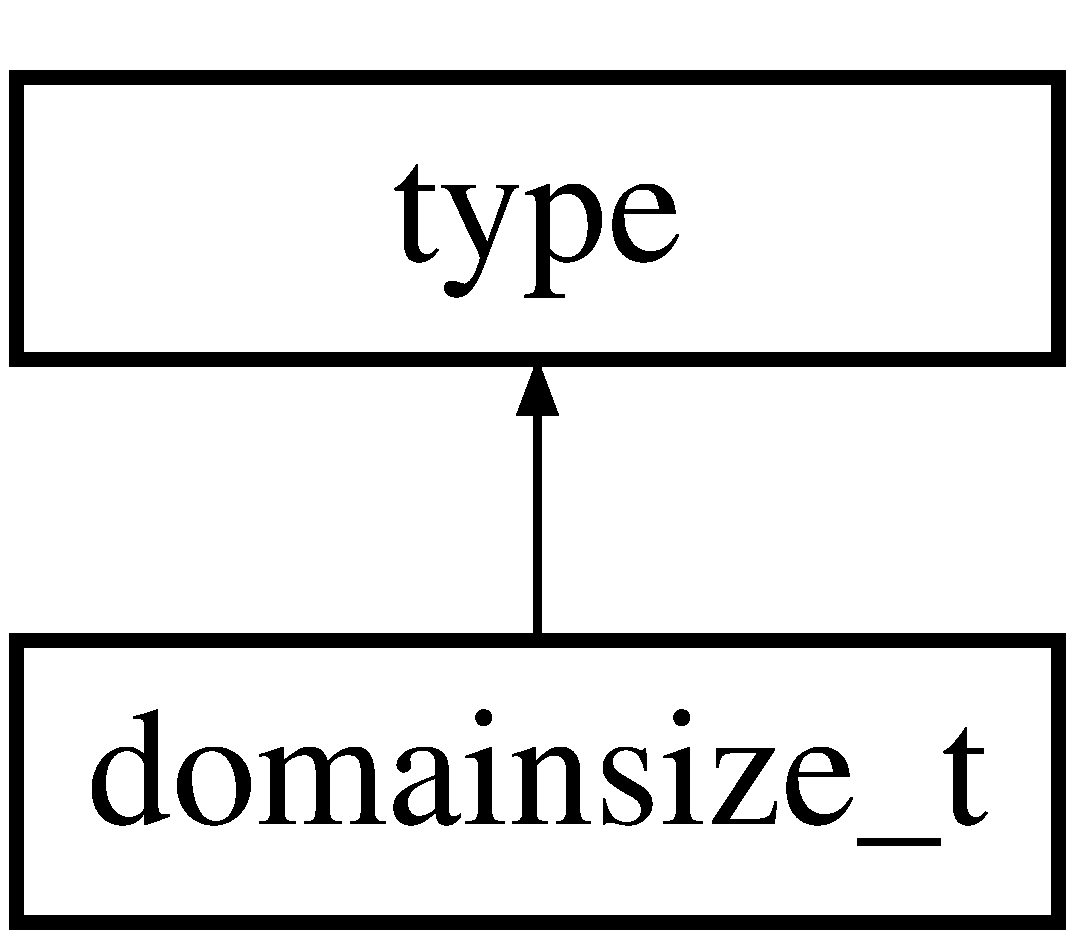
\includegraphics[height=2.000000cm]{classdomainsize__t}
\end{center}
\end{figure}
\subsection*{Public Types}
\begin{DoxyCompactItemize}
\item 
typedef \-::\hyperlink{namespacexml__schema_a69bfaf24f63a8c18ebd8e21db6b343df}{xml\-\_\-schema\-::decimal} \hyperlink{classdomainsize__t_a854a03c90869763fcf75511fadb5caef}{domain\-X\-\_\-type}
\item 
typedef \\*
\-::xsd\-::cxx\-::tree\-::traits\\*
$<$ \hyperlink{classdomainsize__t_a854a03c90869763fcf75511fadb5caef}{domain\-X\-\_\-type}, char,\-::xsd\-::cxx\-::tree\-::schema\-\_\-type\-::decimal $>$ \hyperlink{classdomainsize__t_ab85fcf810949f1a467f81f0f7f443eb4}{domain\-X\-\_\-traits}
\item 
typedef \-::\hyperlink{namespacexml__schema_a69bfaf24f63a8c18ebd8e21db6b343df}{xml\-\_\-schema\-::decimal} \hyperlink{classdomainsize__t_a668c8a71e21505b0ad029fa62f996085}{domain\-Y\-\_\-type}
\item 
typedef \\*
\-::xsd\-::cxx\-::tree\-::traits\\*
$<$ \hyperlink{classdomainsize__t_a668c8a71e21505b0ad029fa62f996085}{domain\-Y\-\_\-type}, char,\-::xsd\-::cxx\-::tree\-::schema\-\_\-type\-::decimal $>$ \hyperlink{classdomainsize__t_a4a4de85f17a3ad6f88f1ee94df83eba5}{domain\-Y\-\_\-traits}
\item 
typedef \-::\hyperlink{namespacexml__schema_a69bfaf24f63a8c18ebd8e21db6b343df}{xml\-\_\-schema\-::decimal} \hyperlink{classdomainsize__t_ab33974c39e210e214cc02d863326cf5c}{domain\-Z\-\_\-type}
\item 
typedef \\*
\-::xsd\-::cxx\-::tree\-::traits\\*
$<$ \hyperlink{classdomainsize__t_ab33974c39e210e214cc02d863326cf5c}{domain\-Z\-\_\-type}, char,\-::xsd\-::cxx\-::tree\-::schema\-\_\-type\-::decimal $>$ \hyperlink{classdomainsize__t_aaa8ff3c9add78b2aa36254ba82bf137e}{domain\-Z\-\_\-traits}
\end{DoxyCompactItemize}
\subsection*{Public Member Functions}
\begin{DoxyCompactItemize}
\item 
const \hyperlink{classdomainsize__t_a854a03c90869763fcf75511fadb5caef}{domain\-X\-\_\-type} \& \hyperlink{classdomainsize__t_af20451fc039e3472ed3e136aa7a461a5}{domain\-X} () const 
\item 
\hyperlink{classdomainsize__t_a854a03c90869763fcf75511fadb5caef}{domain\-X\-\_\-type} \& \hyperlink{classdomainsize__t_a51adb020afa231bfabfdb214748d146c}{domain\-X} ()
\item 
void \hyperlink{classdomainsize__t_a453d5f0fbfdf2a441f42a84c757efb5f}{domain\-X} (const \hyperlink{classdomainsize__t_a854a03c90869763fcf75511fadb5caef}{domain\-X\-\_\-type} \&x)
\item 
const \hyperlink{classdomainsize__t_a668c8a71e21505b0ad029fa62f996085}{domain\-Y\-\_\-type} \& \hyperlink{classdomainsize__t_a8a3e29ee2c5a8fa874fc5b8ea3279fbe}{domain\-Y} () const 
\item 
\hyperlink{classdomainsize__t_a668c8a71e21505b0ad029fa62f996085}{domain\-Y\-\_\-type} \& \hyperlink{classdomainsize__t_a02af32eae86f59729b6e470d29bdf179}{domain\-Y} ()
\item 
void \hyperlink{classdomainsize__t_acb85a302d01748db733e5abaffdfffa7}{domain\-Y} (const \hyperlink{classdomainsize__t_a668c8a71e21505b0ad029fa62f996085}{domain\-Y\-\_\-type} \&x)
\item 
const \hyperlink{classdomainsize__t_ab33974c39e210e214cc02d863326cf5c}{domain\-Z\-\_\-type} \& \hyperlink{classdomainsize__t_a080be013bdf69600372f49a007c376aa}{domain\-Z} () const 
\item 
\hyperlink{classdomainsize__t_ab33974c39e210e214cc02d863326cf5c}{domain\-Z\-\_\-type} \& \hyperlink{classdomainsize__t_a79339a29b7b8305012b25b8d852dccbc}{domain\-Z} ()
\item 
void \hyperlink{classdomainsize__t_a62ddcdb57fd557fd0f7f62df422aee46}{domain\-Z} (const \hyperlink{classdomainsize__t_ab33974c39e210e214cc02d863326cf5c}{domain\-Z\-\_\-type} \&x)
\item 
\hyperlink{classdomainsize__t_a11ff7a4d86e7d942149499f5ac0b35f0}{domainsize\-\_\-t} (const \hyperlink{classdomainsize__t_a854a03c90869763fcf75511fadb5caef}{domain\-X\-\_\-type} \&, const \hyperlink{classdomainsize__t_a668c8a71e21505b0ad029fa62f996085}{domain\-Y\-\_\-type} \&, const \hyperlink{classdomainsize__t_ab33974c39e210e214cc02d863326cf5c}{domain\-Z\-\_\-type} \&)
\item 
\hyperlink{classdomainsize__t_a1e6ae397612df63c580bc53bcd3f3f5b}{domainsize\-\_\-t} (const \-::xercesc\-::\-D\-O\-M\-Element \&e,\-::\hyperlink{namespacexml__schema_a0612287d030cb2732d31a45b258fdc87}{xml\-\_\-schema\-::flags} f=0,\-::\hyperlink{namespacexml__schema_ada9aa30dc722e93ee2ed7243085402a5}{xml\-\_\-schema\-::container} $\ast$c=0)
\item 
\hyperlink{classdomainsize__t_a89b0505c418287452627be4c17ae8438}{domainsize\-\_\-t} (const \hyperlink{classdomainsize__t}{domainsize\-\_\-t} \&x,\-::\hyperlink{namespacexml__schema_a0612287d030cb2732d31a45b258fdc87}{xml\-\_\-schema\-::flags} f=0,\-::\hyperlink{namespacexml__schema_ada9aa30dc722e93ee2ed7243085402a5}{xml\-\_\-schema\-::container} $\ast$c=0)
\item 
virtual \hyperlink{classdomainsize__t}{domainsize\-\_\-t} $\ast$ \hyperlink{classdomainsize__t_a917b20a45a8bc06b9663072c6c8a51e2}{\-\_\-clone} (\-::\hyperlink{namespacexml__schema_a0612287d030cb2732d31a45b258fdc87}{xml\-\_\-schema\-::flags} f=0,\-::\hyperlink{namespacexml__schema_ada9aa30dc722e93ee2ed7243085402a5}{xml\-\_\-schema\-::container} $\ast$c=0) const 
\item 
virtual \hyperlink{classdomainsize__t_a46a1c740a031fa2ad8d79d04a7cec4a8}{$\sim$domainsize\-\_\-t} ()
\end{DoxyCompactItemize}
\subsection*{Protected Member Functions}
\begin{DoxyCompactItemize}
\item 
void \hyperlink{classdomainsize__t_ae6d10ef7bc37fcd486f892ee188f561c}{parse} (\-::xsd\-::cxx\-::xml\-::dom\-::parser$<$ char $>$ \&,\-::\hyperlink{namespacexml__schema_a0612287d030cb2732d31a45b258fdc87}{xml\-\_\-schema\-::flags})
\end{DoxyCompactItemize}
\subsection*{Protected Attributes}
\begin{DoxyCompactItemize}
\item 
\-::xsd\-::cxx\-::tree\-::one\\*
$<$ \hyperlink{classdomainsize__t_a854a03c90869763fcf75511fadb5caef}{domain\-X\-\_\-type} $>$ \hyperlink{classdomainsize__t_ae05d2759ef53f4cd9ae6ee28947c3d57}{domain\-X\-\_\-}
\item 
\-::xsd\-::cxx\-::tree\-::one\\*
$<$ \hyperlink{classdomainsize__t_a668c8a71e21505b0ad029fa62f996085}{domain\-Y\-\_\-type} $>$ \hyperlink{classdomainsize__t_ad11c925754563db906c2a3a40d32edf5}{domain\-Y\-\_\-}
\item 
\-::xsd\-::cxx\-::tree\-::one\\*
$<$ \hyperlink{classdomainsize__t_ab33974c39e210e214cc02d863326cf5c}{domain\-Z\-\_\-type} $>$ \hyperlink{classdomainsize__t_ad4c2bab3295fbed5f23473cc0a560509}{domain\-Z\-\_\-}
\end{DoxyCompactItemize}


\subsection{Member Typedef Documentation}
\hypertarget{classdomainsize__t_ab85fcf810949f1a467f81f0f7f443eb4}{\index{domainsize\-\_\-t@{domainsize\-\_\-t}!domain\-X\-\_\-traits@{domain\-X\-\_\-traits}}
\index{domain\-X\-\_\-traits@{domain\-X\-\_\-traits}!domainsize_t@{domainsize\-\_\-t}}
\subsubsection[{domain\-X\-\_\-traits}]{\setlength{\rightskip}{0pt plus 5cm}typedef \-::xsd\-::cxx\-::tree\-::traits$<$ {\bf domain\-X\-\_\-type}, char, \-::xsd\-::cxx\-::tree\-::schema\-\_\-type\-::decimal $>$ {\bf domainsize\-\_\-t\-::domain\-X\-\_\-traits}}}\label{classdomainsize__t_ab85fcf810949f1a467f81f0f7f443eb4}
\hypertarget{classdomainsize__t_a854a03c90869763fcf75511fadb5caef}{\index{domainsize\-\_\-t@{domainsize\-\_\-t}!domain\-X\-\_\-type@{domain\-X\-\_\-type}}
\index{domain\-X\-\_\-type@{domain\-X\-\_\-type}!domainsize_t@{domainsize\-\_\-t}}
\subsubsection[{domain\-X\-\_\-type}]{\setlength{\rightskip}{0pt plus 5cm}typedef \-::{\bf xml\-\_\-schema\-::decimal} {\bf domainsize\-\_\-t\-::domain\-X\-\_\-type}}}\label{classdomainsize__t_a854a03c90869763fcf75511fadb5caef}
\hypertarget{classdomainsize__t_a4a4de85f17a3ad6f88f1ee94df83eba5}{\index{domainsize\-\_\-t@{domainsize\-\_\-t}!domain\-Y\-\_\-traits@{domain\-Y\-\_\-traits}}
\index{domain\-Y\-\_\-traits@{domain\-Y\-\_\-traits}!domainsize_t@{domainsize\-\_\-t}}
\subsubsection[{domain\-Y\-\_\-traits}]{\setlength{\rightskip}{0pt plus 5cm}typedef \-::xsd\-::cxx\-::tree\-::traits$<$ {\bf domain\-Y\-\_\-type}, char, \-::xsd\-::cxx\-::tree\-::schema\-\_\-type\-::decimal $>$ {\bf domainsize\-\_\-t\-::domain\-Y\-\_\-traits}}}\label{classdomainsize__t_a4a4de85f17a3ad6f88f1ee94df83eba5}
\hypertarget{classdomainsize__t_a668c8a71e21505b0ad029fa62f996085}{\index{domainsize\-\_\-t@{domainsize\-\_\-t}!domain\-Y\-\_\-type@{domain\-Y\-\_\-type}}
\index{domain\-Y\-\_\-type@{domain\-Y\-\_\-type}!domainsize_t@{domainsize\-\_\-t}}
\subsubsection[{domain\-Y\-\_\-type}]{\setlength{\rightskip}{0pt plus 5cm}typedef \-::{\bf xml\-\_\-schema\-::decimal} {\bf domainsize\-\_\-t\-::domain\-Y\-\_\-type}}}\label{classdomainsize__t_a668c8a71e21505b0ad029fa62f996085}
\hypertarget{classdomainsize__t_aaa8ff3c9add78b2aa36254ba82bf137e}{\index{domainsize\-\_\-t@{domainsize\-\_\-t}!domain\-Z\-\_\-traits@{domain\-Z\-\_\-traits}}
\index{domain\-Z\-\_\-traits@{domain\-Z\-\_\-traits}!domainsize_t@{domainsize\-\_\-t}}
\subsubsection[{domain\-Z\-\_\-traits}]{\setlength{\rightskip}{0pt plus 5cm}typedef \-::xsd\-::cxx\-::tree\-::traits$<$ {\bf domain\-Z\-\_\-type}, char, \-::xsd\-::cxx\-::tree\-::schema\-\_\-type\-::decimal $>$ {\bf domainsize\-\_\-t\-::domain\-Z\-\_\-traits}}}\label{classdomainsize__t_aaa8ff3c9add78b2aa36254ba82bf137e}
\hypertarget{classdomainsize__t_ab33974c39e210e214cc02d863326cf5c}{\index{domainsize\-\_\-t@{domainsize\-\_\-t}!domain\-Z\-\_\-type@{domain\-Z\-\_\-type}}
\index{domain\-Z\-\_\-type@{domain\-Z\-\_\-type}!domainsize_t@{domainsize\-\_\-t}}
\subsubsection[{domain\-Z\-\_\-type}]{\setlength{\rightskip}{0pt plus 5cm}typedef \-::{\bf xml\-\_\-schema\-::decimal} {\bf domainsize\-\_\-t\-::domain\-Z\-\_\-type}}}\label{classdomainsize__t_ab33974c39e210e214cc02d863326cf5c}


\subsection{Constructor \& Destructor Documentation}
\hypertarget{classdomainsize__t_a11ff7a4d86e7d942149499f5ac0b35f0}{\index{domainsize\-\_\-t@{domainsize\-\_\-t}!domainsize\-\_\-t@{domainsize\-\_\-t}}
\index{domainsize\-\_\-t@{domainsize\-\_\-t}!domainsize_t@{domainsize\-\_\-t}}
\subsubsection[{domainsize\-\_\-t}]{\setlength{\rightskip}{0pt plus 5cm}domainsize\-\_\-t\-::domainsize\-\_\-t (
\begin{DoxyParamCaption}
\item[{const {\bf domain\-X\-\_\-type} \&}]{domain\-X, }
\item[{const {\bf domain\-Y\-\_\-type} \&}]{domain\-Y, }
\item[{const {\bf domain\-Z\-\_\-type} \&}]{domain\-Z}
\end{DoxyParamCaption}
)}}\label{classdomainsize__t_a11ff7a4d86e7d942149499f5ac0b35f0}
\hypertarget{classdomainsize__t_a1e6ae397612df63c580bc53bcd3f3f5b}{\index{domainsize\-\_\-t@{domainsize\-\_\-t}!domainsize\-\_\-t@{domainsize\-\_\-t}}
\index{domainsize\-\_\-t@{domainsize\-\_\-t}!domainsize_t@{domainsize\-\_\-t}}
\subsubsection[{domainsize\-\_\-t}]{\setlength{\rightskip}{0pt plus 5cm}domainsize\-\_\-t\-::domainsize\-\_\-t (
\begin{DoxyParamCaption}
\item[{const \-::xercesc\-::\-D\-O\-M\-Element \&}]{e, }
\item[{\-::{\bf xml\-\_\-schema\-::flags}}]{f = {\ttfamily 0}, }
\item[{\-::{\bf xml\-\_\-schema\-::container} $\ast$}]{c = {\ttfamily 0}}
\end{DoxyParamCaption}
)}}\label{classdomainsize__t_a1e6ae397612df63c580bc53bcd3f3f5b}
\hypertarget{classdomainsize__t_a89b0505c418287452627be4c17ae8438}{\index{domainsize\-\_\-t@{domainsize\-\_\-t}!domainsize\-\_\-t@{domainsize\-\_\-t}}
\index{domainsize\-\_\-t@{domainsize\-\_\-t}!domainsize_t@{domainsize\-\_\-t}}
\subsubsection[{domainsize\-\_\-t}]{\setlength{\rightskip}{0pt plus 5cm}domainsize\-\_\-t\-::domainsize\-\_\-t (
\begin{DoxyParamCaption}
\item[{const {\bf domainsize\-\_\-t} \&}]{x, }
\item[{\-::{\bf xml\-\_\-schema\-::flags}}]{f = {\ttfamily 0}, }
\item[{\-::{\bf xml\-\_\-schema\-::container} $\ast$}]{c = {\ttfamily 0}}
\end{DoxyParamCaption}
)}}\label{classdomainsize__t_a89b0505c418287452627be4c17ae8438}
\hypertarget{classdomainsize__t_a46a1c740a031fa2ad8d79d04a7cec4a8}{\index{domainsize\-\_\-t@{domainsize\-\_\-t}!$\sim$domainsize\-\_\-t@{$\sim$domainsize\-\_\-t}}
\index{$\sim$domainsize\-\_\-t@{$\sim$domainsize\-\_\-t}!domainsize_t@{domainsize\-\_\-t}}
\subsubsection[{$\sim$domainsize\-\_\-t}]{\setlength{\rightskip}{0pt plus 5cm}domainsize\-\_\-t\-::$\sim$domainsize\-\_\-t (
\begin{DoxyParamCaption}
{}
\end{DoxyParamCaption}
)\hspace{0.3cm}{\ttfamily [virtual]}}}\label{classdomainsize__t_a46a1c740a031fa2ad8d79d04a7cec4a8}


\subsection{Member Function Documentation}
\hypertarget{classdomainsize__t_a917b20a45a8bc06b9663072c6c8a51e2}{\index{domainsize\-\_\-t@{domainsize\-\_\-t}!\-\_\-clone@{\-\_\-clone}}
\index{\-\_\-clone@{\-\_\-clone}!domainsize_t@{domainsize\-\_\-t}}
\subsubsection[{\-\_\-clone}]{\setlength{\rightskip}{0pt plus 5cm}{\bf domainsize\-\_\-t} $\ast$ domainsize\-\_\-t\-::\-\_\-clone (
\begin{DoxyParamCaption}
\item[{\-::{\bf xml\-\_\-schema\-::flags}}]{f = {\ttfamily 0}, }
\item[{\-::{\bf xml\-\_\-schema\-::container} $\ast$}]{c = {\ttfamily 0}}
\end{DoxyParamCaption}
) const\hspace{0.3cm}{\ttfamily [virtual]}}}\label{classdomainsize__t_a917b20a45a8bc06b9663072c6c8a51e2}
\hypertarget{classdomainsize__t_af20451fc039e3472ed3e136aa7a461a5}{\index{domainsize\-\_\-t@{domainsize\-\_\-t}!domain\-X@{domain\-X}}
\index{domain\-X@{domain\-X}!domainsize_t@{domainsize\-\_\-t}}
\subsubsection[{domain\-X}]{\setlength{\rightskip}{0pt plus 5cm}const {\bf domainsize\-\_\-t\-::domain\-X\-\_\-type} \& domainsize\-\_\-t\-::domain\-X (
\begin{DoxyParamCaption}
{}
\end{DoxyParamCaption}
) const}}\label{classdomainsize__t_af20451fc039e3472ed3e136aa7a461a5}
\hypertarget{classdomainsize__t_a51adb020afa231bfabfdb214748d146c}{\index{domainsize\-\_\-t@{domainsize\-\_\-t}!domain\-X@{domain\-X}}
\index{domain\-X@{domain\-X}!domainsize_t@{domainsize\-\_\-t}}
\subsubsection[{domain\-X}]{\setlength{\rightskip}{0pt plus 5cm}{\bf domainsize\-\_\-t\-::domain\-X\-\_\-type} \& domainsize\-\_\-t\-::domain\-X (
\begin{DoxyParamCaption}
{}
\end{DoxyParamCaption}
)}}\label{classdomainsize__t_a51adb020afa231bfabfdb214748d146c}
\hypertarget{classdomainsize__t_a453d5f0fbfdf2a441f42a84c757efb5f}{\index{domainsize\-\_\-t@{domainsize\-\_\-t}!domain\-X@{domain\-X}}
\index{domain\-X@{domain\-X}!domainsize_t@{domainsize\-\_\-t}}
\subsubsection[{domain\-X}]{\setlength{\rightskip}{0pt plus 5cm}void domainsize\-\_\-t\-::domain\-X (
\begin{DoxyParamCaption}
\item[{const {\bf domain\-X\-\_\-type} \&}]{x}
\end{DoxyParamCaption}
)}}\label{classdomainsize__t_a453d5f0fbfdf2a441f42a84c757efb5f}
\hypertarget{classdomainsize__t_a8a3e29ee2c5a8fa874fc5b8ea3279fbe}{\index{domainsize\-\_\-t@{domainsize\-\_\-t}!domain\-Y@{domain\-Y}}
\index{domain\-Y@{domain\-Y}!domainsize_t@{domainsize\-\_\-t}}
\subsubsection[{domain\-Y}]{\setlength{\rightskip}{0pt plus 5cm}const {\bf domainsize\-\_\-t\-::domain\-Y\-\_\-type} \& domainsize\-\_\-t\-::domain\-Y (
\begin{DoxyParamCaption}
{}
\end{DoxyParamCaption}
) const}}\label{classdomainsize__t_a8a3e29ee2c5a8fa874fc5b8ea3279fbe}
\hypertarget{classdomainsize__t_a02af32eae86f59729b6e470d29bdf179}{\index{domainsize\-\_\-t@{domainsize\-\_\-t}!domain\-Y@{domain\-Y}}
\index{domain\-Y@{domain\-Y}!domainsize_t@{domainsize\-\_\-t}}
\subsubsection[{domain\-Y}]{\setlength{\rightskip}{0pt plus 5cm}{\bf domainsize\-\_\-t\-::domain\-Y\-\_\-type} \& domainsize\-\_\-t\-::domain\-Y (
\begin{DoxyParamCaption}
{}
\end{DoxyParamCaption}
)}}\label{classdomainsize__t_a02af32eae86f59729b6e470d29bdf179}
\hypertarget{classdomainsize__t_acb85a302d01748db733e5abaffdfffa7}{\index{domainsize\-\_\-t@{domainsize\-\_\-t}!domain\-Y@{domain\-Y}}
\index{domain\-Y@{domain\-Y}!domainsize_t@{domainsize\-\_\-t}}
\subsubsection[{domain\-Y}]{\setlength{\rightskip}{0pt plus 5cm}void domainsize\-\_\-t\-::domain\-Y (
\begin{DoxyParamCaption}
\item[{const {\bf domain\-Y\-\_\-type} \&}]{x}
\end{DoxyParamCaption}
)}}\label{classdomainsize__t_acb85a302d01748db733e5abaffdfffa7}
\hypertarget{classdomainsize__t_a080be013bdf69600372f49a007c376aa}{\index{domainsize\-\_\-t@{domainsize\-\_\-t}!domain\-Z@{domain\-Z}}
\index{domain\-Z@{domain\-Z}!domainsize_t@{domainsize\-\_\-t}}
\subsubsection[{domain\-Z}]{\setlength{\rightskip}{0pt plus 5cm}const {\bf domainsize\-\_\-t\-::domain\-Z\-\_\-type} \& domainsize\-\_\-t\-::domain\-Z (
\begin{DoxyParamCaption}
{}
\end{DoxyParamCaption}
) const}}\label{classdomainsize__t_a080be013bdf69600372f49a007c376aa}
\hypertarget{classdomainsize__t_a79339a29b7b8305012b25b8d852dccbc}{\index{domainsize\-\_\-t@{domainsize\-\_\-t}!domain\-Z@{domain\-Z}}
\index{domain\-Z@{domain\-Z}!domainsize_t@{domainsize\-\_\-t}}
\subsubsection[{domain\-Z}]{\setlength{\rightskip}{0pt plus 5cm}{\bf domainsize\-\_\-t\-::domain\-Z\-\_\-type} \& domainsize\-\_\-t\-::domain\-Z (
\begin{DoxyParamCaption}
{}
\end{DoxyParamCaption}
)}}\label{classdomainsize__t_a79339a29b7b8305012b25b8d852dccbc}
\hypertarget{classdomainsize__t_a62ddcdb57fd557fd0f7f62df422aee46}{\index{domainsize\-\_\-t@{domainsize\-\_\-t}!domain\-Z@{domain\-Z}}
\index{domain\-Z@{domain\-Z}!domainsize_t@{domainsize\-\_\-t}}
\subsubsection[{domain\-Z}]{\setlength{\rightskip}{0pt plus 5cm}void domainsize\-\_\-t\-::domain\-Z (
\begin{DoxyParamCaption}
\item[{const {\bf domain\-Z\-\_\-type} \&}]{x}
\end{DoxyParamCaption}
)}}\label{classdomainsize__t_a62ddcdb57fd557fd0f7f62df422aee46}
\hypertarget{classdomainsize__t_ae6d10ef7bc37fcd486f892ee188f561c}{\index{domainsize\-\_\-t@{domainsize\-\_\-t}!parse@{parse}}
\index{parse@{parse}!domainsize_t@{domainsize\-\_\-t}}
\subsubsection[{parse}]{\setlength{\rightskip}{0pt plus 5cm}void domainsize\-\_\-t\-::parse (
\begin{DoxyParamCaption}
\item[{\-::xsd\-::cxx\-::xml\-::dom\-::parser$<$ char $>$ \&}]{p, }
\item[{\-::{\bf xml\-\_\-schema\-::flags}}]{f}
\end{DoxyParamCaption}
)\hspace{0.3cm}{\ttfamily [protected]}}}\label{classdomainsize__t_ae6d10ef7bc37fcd486f892ee188f561c}


\subsection{Member Data Documentation}
\hypertarget{classdomainsize__t_ae05d2759ef53f4cd9ae6ee28947c3d57}{\index{domainsize\-\_\-t@{domainsize\-\_\-t}!domain\-X\-\_\-@{domain\-X\-\_\-}}
\index{domain\-X\-\_\-@{domain\-X\-\_\-}!domainsize_t@{domainsize\-\_\-t}}
\subsubsection[{domain\-X\-\_\-}]{\setlength{\rightskip}{0pt plus 5cm}\-::xsd\-::cxx\-::tree\-::one$<$ {\bf domain\-X\-\_\-type} $>$ domainsize\-\_\-t\-::domain\-X\-\_\-\hspace{0.3cm}{\ttfamily [protected]}}}\label{classdomainsize__t_ae05d2759ef53f4cd9ae6ee28947c3d57}
\hypertarget{classdomainsize__t_ad11c925754563db906c2a3a40d32edf5}{\index{domainsize\-\_\-t@{domainsize\-\_\-t}!domain\-Y\-\_\-@{domain\-Y\-\_\-}}
\index{domain\-Y\-\_\-@{domain\-Y\-\_\-}!domainsize_t@{domainsize\-\_\-t}}
\subsubsection[{domain\-Y\-\_\-}]{\setlength{\rightskip}{0pt plus 5cm}\-::xsd\-::cxx\-::tree\-::one$<$ {\bf domain\-Y\-\_\-type} $>$ domainsize\-\_\-t\-::domain\-Y\-\_\-\hspace{0.3cm}{\ttfamily [protected]}}}\label{classdomainsize__t_ad11c925754563db906c2a3a40d32edf5}
\hypertarget{classdomainsize__t_ad4c2bab3295fbed5f23473cc0a560509}{\index{domainsize\-\_\-t@{domainsize\-\_\-t}!domain\-Z\-\_\-@{domain\-Z\-\_\-}}
\index{domain\-Z\-\_\-@{domain\-Z\-\_\-}!domainsize_t@{domainsize\-\_\-t}}
\subsubsection[{domain\-Z\-\_\-}]{\setlength{\rightskip}{0pt plus 5cm}\-::xsd\-::cxx\-::tree\-::one$<$ {\bf domain\-Z\-\_\-type} $>$ domainsize\-\_\-t\-::domain\-Z\-\_\-\hspace{0.3cm}{\ttfamily [protected]}}}\label{classdomainsize__t_ad4c2bab3295fbed5f23473cc0a560509}


The documentation for this class was generated from the following files\-:\begin{DoxyCompactItemize}
\item 
src/utils/\hyperlink{InputSetting_8h}{Input\-Setting.\-h}\item 
src/utils/\hyperlink{InputSetting_8cpp}{Input\-Setting.\-cpp}\end{DoxyCompactItemize}

\hypertarget{classFileReader}{\section{File\-Reader Class Reference}
\label{classFileReader}\index{File\-Reader@{File\-Reader}}
}


{\ttfamily \#include $<$File\-Reader.\-h$>$}

\subsection*{Public Member Functions}
\begin{DoxyCompactItemize}
\item 
\hyperlink{classFileReader_a615dcb2443cad1f2ca123c7c0c334480}{File\-Reader} ()
\item 
virtual \hyperlink{classFileReader_a1382969e8f1468f3b04ad4b44ab39dee}{$\sim$\-File\-Reader} ()
\item 
void \hyperlink{classFileReader_a98e0f676c498629dd005101f399f2a3c}{read\-File} (std\-::list$<$ \hyperlink{classParticle}{Particle} $>$ \&\hyperlink{InputParticles_8h_acc42f43077e01f03478dad72f0e59107}{particles}, char $\ast$filename)
\item 
void \hyperlink{classFileReader_a955bc976be71f48dd87b699c59723726}{read\-File\-Cub} (std\-::list$<$ \hyperlink{classCuboid}{Cuboid} $>$ \&\hyperlink{InputCuboids_8h_a6fbb69a9e0ce5b917daeba332607a1d9}{cuboids}, char $\ast$filename)
\item 
void \hyperlink{classFileReader_a52fabe8d8298aa7d6d3b4c34e20a25bc}{read\-Status} (std\-::list$<$ \hyperlink{classParticle}{Particle} $>$ \&\hyperlink{InputParticles_8h_acc42f43077e01f03478dad72f0e59107}{particles}, double \&eps, double \&sig, char $\ast$filename)
\end{DoxyCompactItemize}


\subsection{Constructor \& Destructor Documentation}
\hypertarget{classFileReader_a615dcb2443cad1f2ca123c7c0c334480}{\index{File\-Reader@{File\-Reader}!File\-Reader@{File\-Reader}}
\index{File\-Reader@{File\-Reader}!FileReader@{File\-Reader}}
\subsubsection[{File\-Reader}]{\setlength{\rightskip}{0pt plus 5cm}File\-Reader\-::\-File\-Reader (
\begin{DoxyParamCaption}
{}
\end{DoxyParamCaption}
)}}\label{classFileReader_a615dcb2443cad1f2ca123c7c0c334480}
\hypertarget{classFileReader_a1382969e8f1468f3b04ad4b44ab39dee}{\index{File\-Reader@{File\-Reader}!$\sim$\-File\-Reader@{$\sim$\-File\-Reader}}
\index{$\sim$\-File\-Reader@{$\sim$\-File\-Reader}!FileReader@{File\-Reader}}
\subsubsection[{$\sim$\-File\-Reader}]{\setlength{\rightskip}{0pt plus 5cm}File\-Reader\-::$\sim$\-File\-Reader (
\begin{DoxyParamCaption}
{}
\end{DoxyParamCaption}
)\hspace{0.3cm}{\ttfamily [virtual]}}}\label{classFileReader_a1382969e8f1468f3b04ad4b44ab39dee}


\subsection{Member Function Documentation}
\hypertarget{classFileReader_a98e0f676c498629dd005101f399f2a3c}{\index{File\-Reader@{File\-Reader}!read\-File@{read\-File}}
\index{read\-File@{read\-File}!FileReader@{File\-Reader}}
\subsubsection[{read\-File}]{\setlength{\rightskip}{0pt plus 5cm}void File\-Reader\-::read\-File (
\begin{DoxyParamCaption}
\item[{std\-::list$<$ {\bf Particle} $>$ \&}]{particles, }
\item[{char $\ast$}]{filename}
\end{DoxyParamCaption}
)}}\label{classFileReader_a98e0f676c498629dd005101f399f2a3c}
\hypertarget{classFileReader_a955bc976be71f48dd87b699c59723726}{\index{File\-Reader@{File\-Reader}!read\-File\-Cub@{read\-File\-Cub}}
\index{read\-File\-Cub@{read\-File\-Cub}!FileReader@{File\-Reader}}
\subsubsection[{read\-File\-Cub}]{\setlength{\rightskip}{0pt plus 5cm}void File\-Reader\-::read\-File\-Cub (
\begin{DoxyParamCaption}
\item[{std\-::list$<$ {\bf Cuboid} $>$ \&}]{cuboids, }
\item[{char $\ast$}]{filename}
\end{DoxyParamCaption}
)}}\label{classFileReader_a955bc976be71f48dd87b699c59723726}
\hypertarget{classFileReader_a52fabe8d8298aa7d6d3b4c34e20a25bc}{\index{File\-Reader@{File\-Reader}!read\-Status@{read\-Status}}
\index{read\-Status@{read\-Status}!FileReader@{File\-Reader}}
\subsubsection[{read\-Status}]{\setlength{\rightskip}{0pt plus 5cm}void File\-Reader\-::read\-Status (
\begin{DoxyParamCaption}
\item[{std\-::list$<$ {\bf Particle} $>$ \&}]{particles, }
\item[{double \&}]{eps, }
\item[{double \&}]{sig, }
\item[{char $\ast$}]{filename}
\end{DoxyParamCaption}
)}}\label{classFileReader_a52fabe8d8298aa7d6d3b4c34e20a25bc}


The documentation for this class was generated from the following files\-:\begin{DoxyCompactItemize}
\item 
src/\hyperlink{FileReader_8h}{File\-Reader.\-h}\item 
src/\hyperlink{FileReader_8cpp}{File\-Reader.\-cpp}\end{DoxyCompactItemize}

\hypertarget{classFileReaderTest}{\section{File\-Reader\-Test Class Reference}
\label{classFileReaderTest}\index{File\-Reader\-Test@{File\-Reader\-Test}}
}


{\ttfamily \#include $<$File\-Reader\-Test.\-h$>$}

Inheritance diagram for File\-Reader\-Test\-:\begin{figure}[H]
\begin{center}
\leavevmode
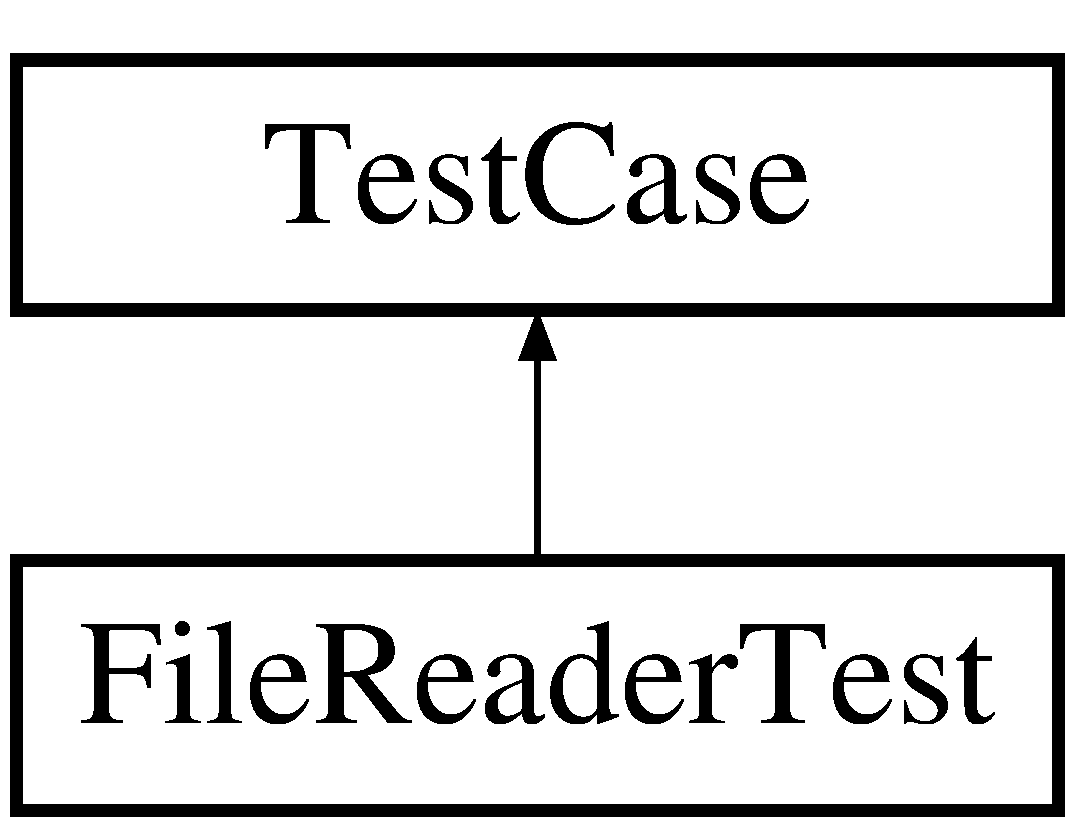
\includegraphics[height=2.000000cm]{classFileReaderTest}
\end{center}
\end{figure}
\subsection*{Public Member Functions}
\begin{DoxyCompactItemize}
\item 
\hyperlink{classFileReaderTest_ac92a30377a8218554355290cb0ae130e}{File\-Reader\-Test} ()
\item 
void \hyperlink{classFileReaderTest_a8bb8664fa4d0e49718bb9ba817fa771d}{set\-Up} ()
\item 
void \hyperlink{classFileReaderTest_ada74df1e362f734c57ee89f7bf53e521}{tear\-Down} ()
\item 
void \hyperlink{classFileReaderTest_aaf0cd61b9bd03ae16b5352510de97aa6}{test\-Read\-Status} ()
\item 
virtual \hyperlink{classFileReaderTest_aeb69bbc38884c819cfd68ac750d7fdb3}{$\sim$\-File\-Reader\-Test} ()
\end{DoxyCompactItemize}
\subsection*{Static Public Member Functions}
\begin{DoxyCompactItemize}
\item 
static Test $\ast$ \hyperlink{classFileReaderTest_ab8f863433805210e5eb463c961d3c3bc}{suite} ()
\end{DoxyCompactItemize}
\subsection*{Private Attributes}
\begin{DoxyCompactItemize}
\item 
std\-::list$<$ \hyperlink{classParticle}{Particle} $>$ \hyperlink{classFileReaderTest_a9392293a0d47f08bee440ea1b4c5925a}{test\-L}
\end{DoxyCompactItemize}


\subsection{Constructor \& Destructor Documentation}
\hypertarget{classFileReaderTest_ac92a30377a8218554355290cb0ae130e}{\index{File\-Reader\-Test@{File\-Reader\-Test}!File\-Reader\-Test@{File\-Reader\-Test}}
\index{File\-Reader\-Test@{File\-Reader\-Test}!FileReaderTest@{File\-Reader\-Test}}
\subsubsection[{File\-Reader\-Test}]{\setlength{\rightskip}{0pt plus 5cm}File\-Reader\-Test\-::\-File\-Reader\-Test (
\begin{DoxyParamCaption}
{}
\end{DoxyParamCaption}
)}}\label{classFileReaderTest_ac92a30377a8218554355290cb0ae130e}
\hypertarget{classFileReaderTest_aeb69bbc38884c819cfd68ac750d7fdb3}{\index{File\-Reader\-Test@{File\-Reader\-Test}!$\sim$\-File\-Reader\-Test@{$\sim$\-File\-Reader\-Test}}
\index{$\sim$\-File\-Reader\-Test@{$\sim$\-File\-Reader\-Test}!FileReaderTest@{File\-Reader\-Test}}
\subsubsection[{$\sim$\-File\-Reader\-Test}]{\setlength{\rightskip}{0pt plus 5cm}File\-Reader\-Test\-::$\sim$\-File\-Reader\-Test (
\begin{DoxyParamCaption}
{}
\end{DoxyParamCaption}
)\hspace{0.3cm}{\ttfamily [virtual]}}}\label{classFileReaderTest_aeb69bbc38884c819cfd68ac750d7fdb3}


\subsection{Member Function Documentation}
\hypertarget{classFileReaderTest_a8bb8664fa4d0e49718bb9ba817fa771d}{\index{File\-Reader\-Test@{File\-Reader\-Test}!set\-Up@{set\-Up}}
\index{set\-Up@{set\-Up}!FileReaderTest@{File\-Reader\-Test}}
\subsubsection[{set\-Up}]{\setlength{\rightskip}{0pt plus 5cm}void File\-Reader\-Test\-::set\-Up (
\begin{DoxyParamCaption}
{}
\end{DoxyParamCaption}
)}}\label{classFileReaderTest_a8bb8664fa4d0e49718bb9ba817fa771d}
\hypertarget{classFileReaderTest_ab8f863433805210e5eb463c961d3c3bc}{\index{File\-Reader\-Test@{File\-Reader\-Test}!suite@{suite}}
\index{suite@{suite}!FileReaderTest@{File\-Reader\-Test}}
\subsubsection[{suite}]{\setlength{\rightskip}{0pt plus 5cm}Cpp\-Unit\-::\-Test $\ast$ File\-Reader\-Test\-::suite (
\begin{DoxyParamCaption}
{}
\end{DoxyParamCaption}
)\hspace{0.3cm}{\ttfamily [static]}}}\label{classFileReaderTest_ab8f863433805210e5eb463c961d3c3bc}
\hypertarget{classFileReaderTest_ada74df1e362f734c57ee89f7bf53e521}{\index{File\-Reader\-Test@{File\-Reader\-Test}!tear\-Down@{tear\-Down}}
\index{tear\-Down@{tear\-Down}!FileReaderTest@{File\-Reader\-Test}}
\subsubsection[{tear\-Down}]{\setlength{\rightskip}{0pt plus 5cm}void File\-Reader\-Test\-::tear\-Down (
\begin{DoxyParamCaption}
{}
\end{DoxyParamCaption}
)}}\label{classFileReaderTest_ada74df1e362f734c57ee89f7bf53e521}
\hypertarget{classFileReaderTest_aaf0cd61b9bd03ae16b5352510de97aa6}{\index{File\-Reader\-Test@{File\-Reader\-Test}!test\-Read\-Status@{test\-Read\-Status}}
\index{test\-Read\-Status@{test\-Read\-Status}!FileReaderTest@{File\-Reader\-Test}}
\subsubsection[{test\-Read\-Status}]{\setlength{\rightskip}{0pt plus 5cm}void File\-Reader\-Test\-::test\-Read\-Status (
\begin{DoxyParamCaption}
{}
\end{DoxyParamCaption}
)}}\label{classFileReaderTest_aaf0cd61b9bd03ae16b5352510de97aa6}


\subsection{Member Data Documentation}
\hypertarget{classFileReaderTest_a9392293a0d47f08bee440ea1b4c5925a}{\index{File\-Reader\-Test@{File\-Reader\-Test}!test\-L@{test\-L}}
\index{test\-L@{test\-L}!FileReaderTest@{File\-Reader\-Test}}
\subsubsection[{test\-L}]{\setlength{\rightskip}{0pt plus 5cm}std\-::list$<${\bf Particle}$>$ File\-Reader\-Test\-::test\-L\hspace{0.3cm}{\ttfamily [private]}}}\label{classFileReaderTest_a9392293a0d47f08bee440ea1b4c5925a}


The documentation for this class was generated from the following files\-:\begin{DoxyCompactItemize}
\item 
src/tests/\hyperlink{FileReaderTest_8h}{File\-Reader\-Test.\-h}\item 
src/tests/\hyperlink{FileReaderTest_8cpp}{File\-Reader\-Test.\-cpp}\end{DoxyCompactItemize}

\hypertarget{classinputfile__t}{\section{inputfile\-\_\-t Class Reference}
\label{classinputfile__t}\index{inputfile\-\_\-t@{inputfile\-\_\-t}}
}


{\ttfamily \#include $<$Input\-Setting.\-h$>$}

Inheritance diagram for inputfile\-\_\-t\-:\begin{figure}[H]
\begin{center}
\leavevmode
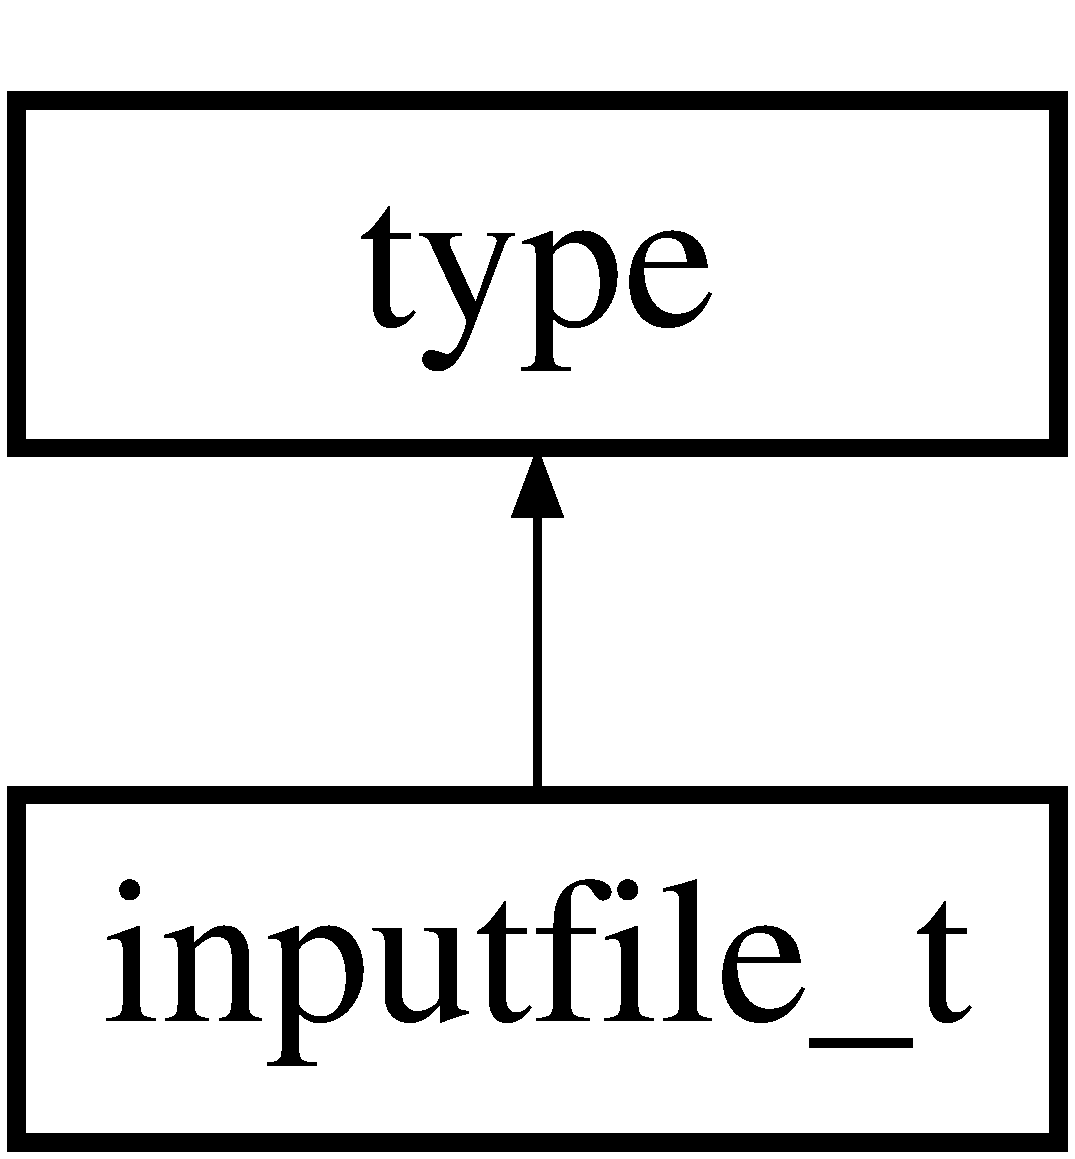
\includegraphics[height=2.000000cm]{classinputfile__t}
\end{center}
\end{figure}
\subsection*{Public Types}
\begin{DoxyCompactItemize}
\item 
typedef \-::\hyperlink{namespacexml__schema_ac0cec83a330f0024e4e318b3deac5104}{xml\-\_\-schema\-::string} \hyperlink{classinputfile__t_a78bf4131e7e2a433bfe95f85b2a5e1da}{name\-\_\-type}
\item 
typedef \\*
\-::xsd\-::cxx\-::tree\-::traits\\*
$<$ \hyperlink{classinputfile__t_a78bf4131e7e2a433bfe95f85b2a5e1da}{name\-\_\-type}, char $>$ \hyperlink{classinputfile__t_a7d5c68e89634f1ebe16b33a42d43ea50}{name\-\_\-traits}
\item 
typedef \-::\hyperlink{classtype__t}{type\-\_\-t} \hyperlink{classinputfile__t_a3f28e99146a586a8f55154818cdfe1ad}{type\-\_\-type}
\item 
typedef \\*
\-::xsd\-::cxx\-::tree\-::traits\\*
$<$ \hyperlink{classinputfile__t_a3f28e99146a586a8f55154818cdfe1ad}{type\-\_\-type}, char $>$ \hyperlink{classinputfile__t_abcbf4050c7030f43da48c567d60444ae}{type\-\_\-traits}
\end{DoxyCompactItemize}
\subsection*{Public Member Functions}
\begin{DoxyCompactItemize}
\item 
const \hyperlink{classinputfile__t_a78bf4131e7e2a433bfe95f85b2a5e1da}{name\-\_\-type} \& \hyperlink{classinputfile__t_a421b173ebce0a604ecc24e7144bebfd1}{name} () const 
\item 
\hyperlink{classinputfile__t_a78bf4131e7e2a433bfe95f85b2a5e1da}{name\-\_\-type} \& \hyperlink{classinputfile__t_af07afab2e4b5fcfded1980b068f47648}{name} ()
\item 
void \hyperlink{classinputfile__t_ab64c88264ed68fd54807a62853994662}{name} (const \hyperlink{classinputfile__t_a78bf4131e7e2a433bfe95f85b2a5e1da}{name\-\_\-type} \&x)
\item 
void \hyperlink{classinputfile__t_ab0fd338383c85ac998025f4f0c10d63f}{name} (\-::std\-::auto\-\_\-ptr$<$ \hyperlink{classinputfile__t_a78bf4131e7e2a433bfe95f85b2a5e1da}{name\-\_\-type} $>$ p)
\item 
const \hyperlink{classinputfile__t_a3f28e99146a586a8f55154818cdfe1ad}{type\-\_\-type} \& \hyperlink{classinputfile__t_a365e0471f78ac9f457471f93a44093dc}{type} () const 
\item 
\hyperlink{classinputfile__t_a3f28e99146a586a8f55154818cdfe1ad}{type\-\_\-type} \& \hyperlink{classinputfile__t_a17a37451ba128f3f05eeef4a80a84193}{type} ()
\item 
void \hyperlink{classinputfile__t_a0308f273b0ee4c4d687bbc33ccdb3b0c}{type} (const \hyperlink{classinputfile__t_a3f28e99146a586a8f55154818cdfe1ad}{type\-\_\-type} \&x)
\item 
void \hyperlink{classinputfile__t_a5f1a595db6d70d79d173a63511a45a6b}{type} (\-::std\-::auto\-\_\-ptr$<$ \hyperlink{classinputfile__t_a3f28e99146a586a8f55154818cdfe1ad}{type\-\_\-type} $>$ p)
\item 
\hyperlink{classinputfile__t_ac5caf96746fcce27a5636c2decb4979b}{inputfile\-\_\-t} (const \hyperlink{classinputfile__t_a78bf4131e7e2a433bfe95f85b2a5e1da}{name\-\_\-type} \&, const \hyperlink{classinputfile__t_a3f28e99146a586a8f55154818cdfe1ad}{type\-\_\-type} \&)
\item 
\hyperlink{classinputfile__t_a818f579ee694957e72740e373848fca5}{inputfile\-\_\-t} (const \-::xercesc\-::\-D\-O\-M\-Element \&e,\-::\hyperlink{namespacexml__schema_a0612287d030cb2732d31a45b258fdc87}{xml\-\_\-schema\-::flags} f=0,\-::\hyperlink{namespacexml__schema_ada9aa30dc722e93ee2ed7243085402a5}{xml\-\_\-schema\-::container} $\ast$c=0)
\item 
\hyperlink{classinputfile__t_a6faa9460f16ce6f4d19e5482301d21bb}{inputfile\-\_\-t} (const \hyperlink{classinputfile__t}{inputfile\-\_\-t} \&x,\-::\hyperlink{namespacexml__schema_a0612287d030cb2732d31a45b258fdc87}{xml\-\_\-schema\-::flags} f=0,\-::\hyperlink{namespacexml__schema_ada9aa30dc722e93ee2ed7243085402a5}{xml\-\_\-schema\-::container} $\ast$c=0)
\item 
virtual \hyperlink{classinputfile__t}{inputfile\-\_\-t} $\ast$ \hyperlink{classinputfile__t_ad5a888bcf78e692a206899e5fb64074c}{\-\_\-clone} (\-::\hyperlink{namespacexml__schema_a0612287d030cb2732d31a45b258fdc87}{xml\-\_\-schema\-::flags} f=0,\-::\hyperlink{namespacexml__schema_ada9aa30dc722e93ee2ed7243085402a5}{xml\-\_\-schema\-::container} $\ast$c=0) const 
\item 
virtual \hyperlink{classinputfile__t_a51d305c8e979f80d0430333b3663211d}{$\sim$inputfile\-\_\-t} ()
\end{DoxyCompactItemize}
\subsection*{Protected Member Functions}
\begin{DoxyCompactItemize}
\item 
void \hyperlink{classinputfile__t_a456996966d112692aef85483b0e388e3}{parse} (\-::xsd\-::cxx\-::xml\-::dom\-::parser$<$ char $>$ \&,\-::\hyperlink{namespacexml__schema_a0612287d030cb2732d31a45b258fdc87}{xml\-\_\-schema\-::flags})
\end{DoxyCompactItemize}
\subsection*{Protected Attributes}
\begin{DoxyCompactItemize}
\item 
\-::xsd\-::cxx\-::tree\-::one$<$ \hyperlink{classinputfile__t_a78bf4131e7e2a433bfe95f85b2a5e1da}{name\-\_\-type} $>$ \hyperlink{classinputfile__t_a511fa53cd30df30388bbb0d6667e04e5}{name\-\_\-}
\item 
\-::xsd\-::cxx\-::tree\-::one$<$ \hyperlink{classinputfile__t_a3f28e99146a586a8f55154818cdfe1ad}{type\-\_\-type} $>$ \hyperlink{classinputfile__t_aac635b58fd41459baf72cb928c4f41b1}{type\-\_\-}
\end{DoxyCompactItemize}


\subsection{Member Typedef Documentation}
\hypertarget{classinputfile__t_a7d5c68e89634f1ebe16b33a42d43ea50}{\index{inputfile\-\_\-t@{inputfile\-\_\-t}!name\-\_\-traits@{name\-\_\-traits}}
\index{name\-\_\-traits@{name\-\_\-traits}!inputfile_t@{inputfile\-\_\-t}}
\subsubsection[{name\-\_\-traits}]{\setlength{\rightskip}{0pt plus 5cm}typedef \-::xsd\-::cxx\-::tree\-::traits$<$ {\bf name\-\_\-type}, char $>$ {\bf inputfile\-\_\-t\-::name\-\_\-traits}}}\label{classinputfile__t_a7d5c68e89634f1ebe16b33a42d43ea50}
\hypertarget{classinputfile__t_a78bf4131e7e2a433bfe95f85b2a5e1da}{\index{inputfile\-\_\-t@{inputfile\-\_\-t}!name\-\_\-type@{name\-\_\-type}}
\index{name\-\_\-type@{name\-\_\-type}!inputfile_t@{inputfile\-\_\-t}}
\subsubsection[{name\-\_\-type}]{\setlength{\rightskip}{0pt plus 5cm}typedef \-::{\bf xml\-\_\-schema\-::string} {\bf inputfile\-\_\-t\-::name\-\_\-type}}}\label{classinputfile__t_a78bf4131e7e2a433bfe95f85b2a5e1da}
\hypertarget{classinputfile__t_abcbf4050c7030f43da48c567d60444ae}{\index{inputfile\-\_\-t@{inputfile\-\_\-t}!type\-\_\-traits@{type\-\_\-traits}}
\index{type\-\_\-traits@{type\-\_\-traits}!inputfile_t@{inputfile\-\_\-t}}
\subsubsection[{type\-\_\-traits}]{\setlength{\rightskip}{0pt plus 5cm}typedef \-::xsd\-::cxx\-::tree\-::traits$<$ {\bf type\-\_\-type}, char $>$ {\bf inputfile\-\_\-t\-::type\-\_\-traits}}}\label{classinputfile__t_abcbf4050c7030f43da48c567d60444ae}
\hypertarget{classinputfile__t_a3f28e99146a586a8f55154818cdfe1ad}{\index{inputfile\-\_\-t@{inputfile\-\_\-t}!type\-\_\-type@{type\-\_\-type}}
\index{type\-\_\-type@{type\-\_\-type}!inputfile_t@{inputfile\-\_\-t}}
\subsubsection[{type\-\_\-type}]{\setlength{\rightskip}{0pt plus 5cm}typedef \-::{\bf type\-\_\-t} {\bf inputfile\-\_\-t\-::type\-\_\-type}}}\label{classinputfile__t_a3f28e99146a586a8f55154818cdfe1ad}


\subsection{Constructor \& Destructor Documentation}
\hypertarget{classinputfile__t_ac5caf96746fcce27a5636c2decb4979b}{\index{inputfile\-\_\-t@{inputfile\-\_\-t}!inputfile\-\_\-t@{inputfile\-\_\-t}}
\index{inputfile\-\_\-t@{inputfile\-\_\-t}!inputfile_t@{inputfile\-\_\-t}}
\subsubsection[{inputfile\-\_\-t}]{\setlength{\rightskip}{0pt plus 5cm}inputfile\-\_\-t\-::inputfile\-\_\-t (
\begin{DoxyParamCaption}
\item[{const {\bf name\-\_\-type} \&}]{name, }
\item[{const {\bf type\-\_\-type} \&}]{type}
\end{DoxyParamCaption}
)}}\label{classinputfile__t_ac5caf96746fcce27a5636c2decb4979b}
\hypertarget{classinputfile__t_a818f579ee694957e72740e373848fca5}{\index{inputfile\-\_\-t@{inputfile\-\_\-t}!inputfile\-\_\-t@{inputfile\-\_\-t}}
\index{inputfile\-\_\-t@{inputfile\-\_\-t}!inputfile_t@{inputfile\-\_\-t}}
\subsubsection[{inputfile\-\_\-t}]{\setlength{\rightskip}{0pt plus 5cm}inputfile\-\_\-t\-::inputfile\-\_\-t (
\begin{DoxyParamCaption}
\item[{const \-::xercesc\-::\-D\-O\-M\-Element \&}]{e, }
\item[{\-::{\bf xml\-\_\-schema\-::flags}}]{f = {\ttfamily 0}, }
\item[{\-::{\bf xml\-\_\-schema\-::container} $\ast$}]{c = {\ttfamily 0}}
\end{DoxyParamCaption}
)}}\label{classinputfile__t_a818f579ee694957e72740e373848fca5}
\hypertarget{classinputfile__t_a6faa9460f16ce6f4d19e5482301d21bb}{\index{inputfile\-\_\-t@{inputfile\-\_\-t}!inputfile\-\_\-t@{inputfile\-\_\-t}}
\index{inputfile\-\_\-t@{inputfile\-\_\-t}!inputfile_t@{inputfile\-\_\-t}}
\subsubsection[{inputfile\-\_\-t}]{\setlength{\rightskip}{0pt plus 5cm}inputfile\-\_\-t\-::inputfile\-\_\-t (
\begin{DoxyParamCaption}
\item[{const {\bf inputfile\-\_\-t} \&}]{x, }
\item[{\-::{\bf xml\-\_\-schema\-::flags}}]{f = {\ttfamily 0}, }
\item[{\-::{\bf xml\-\_\-schema\-::container} $\ast$}]{c = {\ttfamily 0}}
\end{DoxyParamCaption}
)}}\label{classinputfile__t_a6faa9460f16ce6f4d19e5482301d21bb}
\hypertarget{classinputfile__t_a51d305c8e979f80d0430333b3663211d}{\index{inputfile\-\_\-t@{inputfile\-\_\-t}!$\sim$inputfile\-\_\-t@{$\sim$inputfile\-\_\-t}}
\index{$\sim$inputfile\-\_\-t@{$\sim$inputfile\-\_\-t}!inputfile_t@{inputfile\-\_\-t}}
\subsubsection[{$\sim$inputfile\-\_\-t}]{\setlength{\rightskip}{0pt plus 5cm}inputfile\-\_\-t\-::$\sim$inputfile\-\_\-t (
\begin{DoxyParamCaption}
{}
\end{DoxyParamCaption}
)\hspace{0.3cm}{\ttfamily [virtual]}}}\label{classinputfile__t_a51d305c8e979f80d0430333b3663211d}


\subsection{Member Function Documentation}
\hypertarget{classinputfile__t_ad5a888bcf78e692a206899e5fb64074c}{\index{inputfile\-\_\-t@{inputfile\-\_\-t}!\-\_\-clone@{\-\_\-clone}}
\index{\-\_\-clone@{\-\_\-clone}!inputfile_t@{inputfile\-\_\-t}}
\subsubsection[{\-\_\-clone}]{\setlength{\rightskip}{0pt plus 5cm}{\bf inputfile\-\_\-t} $\ast$ inputfile\-\_\-t\-::\-\_\-clone (
\begin{DoxyParamCaption}
\item[{\-::{\bf xml\-\_\-schema\-::flags}}]{f = {\ttfamily 0}, }
\item[{\-::{\bf xml\-\_\-schema\-::container} $\ast$}]{c = {\ttfamily 0}}
\end{DoxyParamCaption}
) const\hspace{0.3cm}{\ttfamily [virtual]}}}\label{classinputfile__t_ad5a888bcf78e692a206899e5fb64074c}
\hypertarget{classinputfile__t_a421b173ebce0a604ecc24e7144bebfd1}{\index{inputfile\-\_\-t@{inputfile\-\_\-t}!name@{name}}
\index{name@{name}!inputfile_t@{inputfile\-\_\-t}}
\subsubsection[{name}]{\setlength{\rightskip}{0pt plus 5cm}const {\bf inputfile\-\_\-t\-::name\-\_\-type} \& inputfile\-\_\-t\-::name (
\begin{DoxyParamCaption}
{}
\end{DoxyParamCaption}
) const}}\label{classinputfile__t_a421b173ebce0a604ecc24e7144bebfd1}
\hypertarget{classinputfile__t_af07afab2e4b5fcfded1980b068f47648}{\index{inputfile\-\_\-t@{inputfile\-\_\-t}!name@{name}}
\index{name@{name}!inputfile_t@{inputfile\-\_\-t}}
\subsubsection[{name}]{\setlength{\rightskip}{0pt plus 5cm}{\bf inputfile\-\_\-t\-::name\-\_\-type} \& inputfile\-\_\-t\-::name (
\begin{DoxyParamCaption}
{}
\end{DoxyParamCaption}
)}}\label{classinputfile__t_af07afab2e4b5fcfded1980b068f47648}
\hypertarget{classinputfile__t_ab64c88264ed68fd54807a62853994662}{\index{inputfile\-\_\-t@{inputfile\-\_\-t}!name@{name}}
\index{name@{name}!inputfile_t@{inputfile\-\_\-t}}
\subsubsection[{name}]{\setlength{\rightskip}{0pt plus 5cm}void inputfile\-\_\-t\-::name (
\begin{DoxyParamCaption}
\item[{const {\bf name\-\_\-type} \&}]{x}
\end{DoxyParamCaption}
)}}\label{classinputfile__t_ab64c88264ed68fd54807a62853994662}
\hypertarget{classinputfile__t_ab0fd338383c85ac998025f4f0c10d63f}{\index{inputfile\-\_\-t@{inputfile\-\_\-t}!name@{name}}
\index{name@{name}!inputfile_t@{inputfile\-\_\-t}}
\subsubsection[{name}]{\setlength{\rightskip}{0pt plus 5cm}void inputfile\-\_\-t\-::name (
\begin{DoxyParamCaption}
\item[{\-::std\-::auto\-\_\-ptr$<$ {\bf name\-\_\-type} $>$}]{p}
\end{DoxyParamCaption}
)}}\label{classinputfile__t_ab0fd338383c85ac998025f4f0c10d63f}
\hypertarget{classinputfile__t_a456996966d112692aef85483b0e388e3}{\index{inputfile\-\_\-t@{inputfile\-\_\-t}!parse@{parse}}
\index{parse@{parse}!inputfile_t@{inputfile\-\_\-t}}
\subsubsection[{parse}]{\setlength{\rightskip}{0pt plus 5cm}void inputfile\-\_\-t\-::parse (
\begin{DoxyParamCaption}
\item[{\-::xsd\-::cxx\-::xml\-::dom\-::parser$<$ char $>$ \&}]{p, }
\item[{\-::{\bf xml\-\_\-schema\-::flags}}]{f}
\end{DoxyParamCaption}
)\hspace{0.3cm}{\ttfamily [protected]}}}\label{classinputfile__t_a456996966d112692aef85483b0e388e3}
\hypertarget{classinputfile__t_a365e0471f78ac9f457471f93a44093dc}{\index{inputfile\-\_\-t@{inputfile\-\_\-t}!type@{type}}
\index{type@{type}!inputfile_t@{inputfile\-\_\-t}}
\subsubsection[{type}]{\setlength{\rightskip}{0pt plus 5cm}const {\bf inputfile\-\_\-t\-::type\-\_\-type} \& inputfile\-\_\-t\-::type (
\begin{DoxyParamCaption}
{}
\end{DoxyParamCaption}
) const}}\label{classinputfile__t_a365e0471f78ac9f457471f93a44093dc}
\hypertarget{classinputfile__t_a17a37451ba128f3f05eeef4a80a84193}{\index{inputfile\-\_\-t@{inputfile\-\_\-t}!type@{type}}
\index{type@{type}!inputfile_t@{inputfile\-\_\-t}}
\subsubsection[{type}]{\setlength{\rightskip}{0pt plus 5cm}{\bf inputfile\-\_\-t\-::type\-\_\-type} \& inputfile\-\_\-t\-::type (
\begin{DoxyParamCaption}
{}
\end{DoxyParamCaption}
)}}\label{classinputfile__t_a17a37451ba128f3f05eeef4a80a84193}
\hypertarget{classinputfile__t_a0308f273b0ee4c4d687bbc33ccdb3b0c}{\index{inputfile\-\_\-t@{inputfile\-\_\-t}!type@{type}}
\index{type@{type}!inputfile_t@{inputfile\-\_\-t}}
\subsubsection[{type}]{\setlength{\rightskip}{0pt plus 5cm}void inputfile\-\_\-t\-::type (
\begin{DoxyParamCaption}
\item[{const {\bf type\-\_\-type} \&}]{x}
\end{DoxyParamCaption}
)}}\label{classinputfile__t_a0308f273b0ee4c4d687bbc33ccdb3b0c}
\hypertarget{classinputfile__t_a5f1a595db6d70d79d173a63511a45a6b}{\index{inputfile\-\_\-t@{inputfile\-\_\-t}!type@{type}}
\index{type@{type}!inputfile_t@{inputfile\-\_\-t}}
\subsubsection[{type}]{\setlength{\rightskip}{0pt plus 5cm}void inputfile\-\_\-t\-::type (
\begin{DoxyParamCaption}
\item[{\-::std\-::auto\-\_\-ptr$<$ {\bf type\-\_\-type} $>$}]{p}
\end{DoxyParamCaption}
)}}\label{classinputfile__t_a5f1a595db6d70d79d173a63511a45a6b}


\subsection{Member Data Documentation}
\hypertarget{classinputfile__t_a511fa53cd30df30388bbb0d6667e04e5}{\index{inputfile\-\_\-t@{inputfile\-\_\-t}!name\-\_\-@{name\-\_\-}}
\index{name\-\_\-@{name\-\_\-}!inputfile_t@{inputfile\-\_\-t}}
\subsubsection[{name\-\_\-}]{\setlength{\rightskip}{0pt plus 5cm}\-::xsd\-::cxx\-::tree\-::one$<$ {\bf name\-\_\-type} $>$ inputfile\-\_\-t\-::name\-\_\-\hspace{0.3cm}{\ttfamily [protected]}}}\label{classinputfile__t_a511fa53cd30df30388bbb0d6667e04e5}
\hypertarget{classinputfile__t_aac635b58fd41459baf72cb928c4f41b1}{\index{inputfile\-\_\-t@{inputfile\-\_\-t}!type\-\_\-@{type\-\_\-}}
\index{type\-\_\-@{type\-\_\-}!inputfile_t@{inputfile\-\_\-t}}
\subsubsection[{type\-\_\-}]{\setlength{\rightskip}{0pt plus 5cm}\-::xsd\-::cxx\-::tree\-::one$<$ {\bf type\-\_\-type} $>$ inputfile\-\_\-t\-::type\-\_\-\hspace{0.3cm}{\ttfamily [protected]}}}\label{classinputfile__t_aac635b58fd41459baf72cb928c4f41b1}


The documentation for this class was generated from the following files\-:\begin{DoxyCompactItemize}
\item 
src/utils/\hyperlink{InputSetting_8h}{Input\-Setting.\-h}\item 
src/utils/\hyperlink{InputSetting_8cpp}{Input\-Setting.\-cpp}\end{DoxyCompactItemize}

\hypertarget{classlc__t}{\section{lc\-\_\-t Class Reference}
\label{classlc__t}\index{lc\-\_\-t@{lc\-\_\-t}}
}


{\ttfamily \#include $<$Input\-Setting.\-h$>$}

Inheritance diagram for lc\-\_\-t\-:\begin{figure}[H]
\begin{center}
\leavevmode
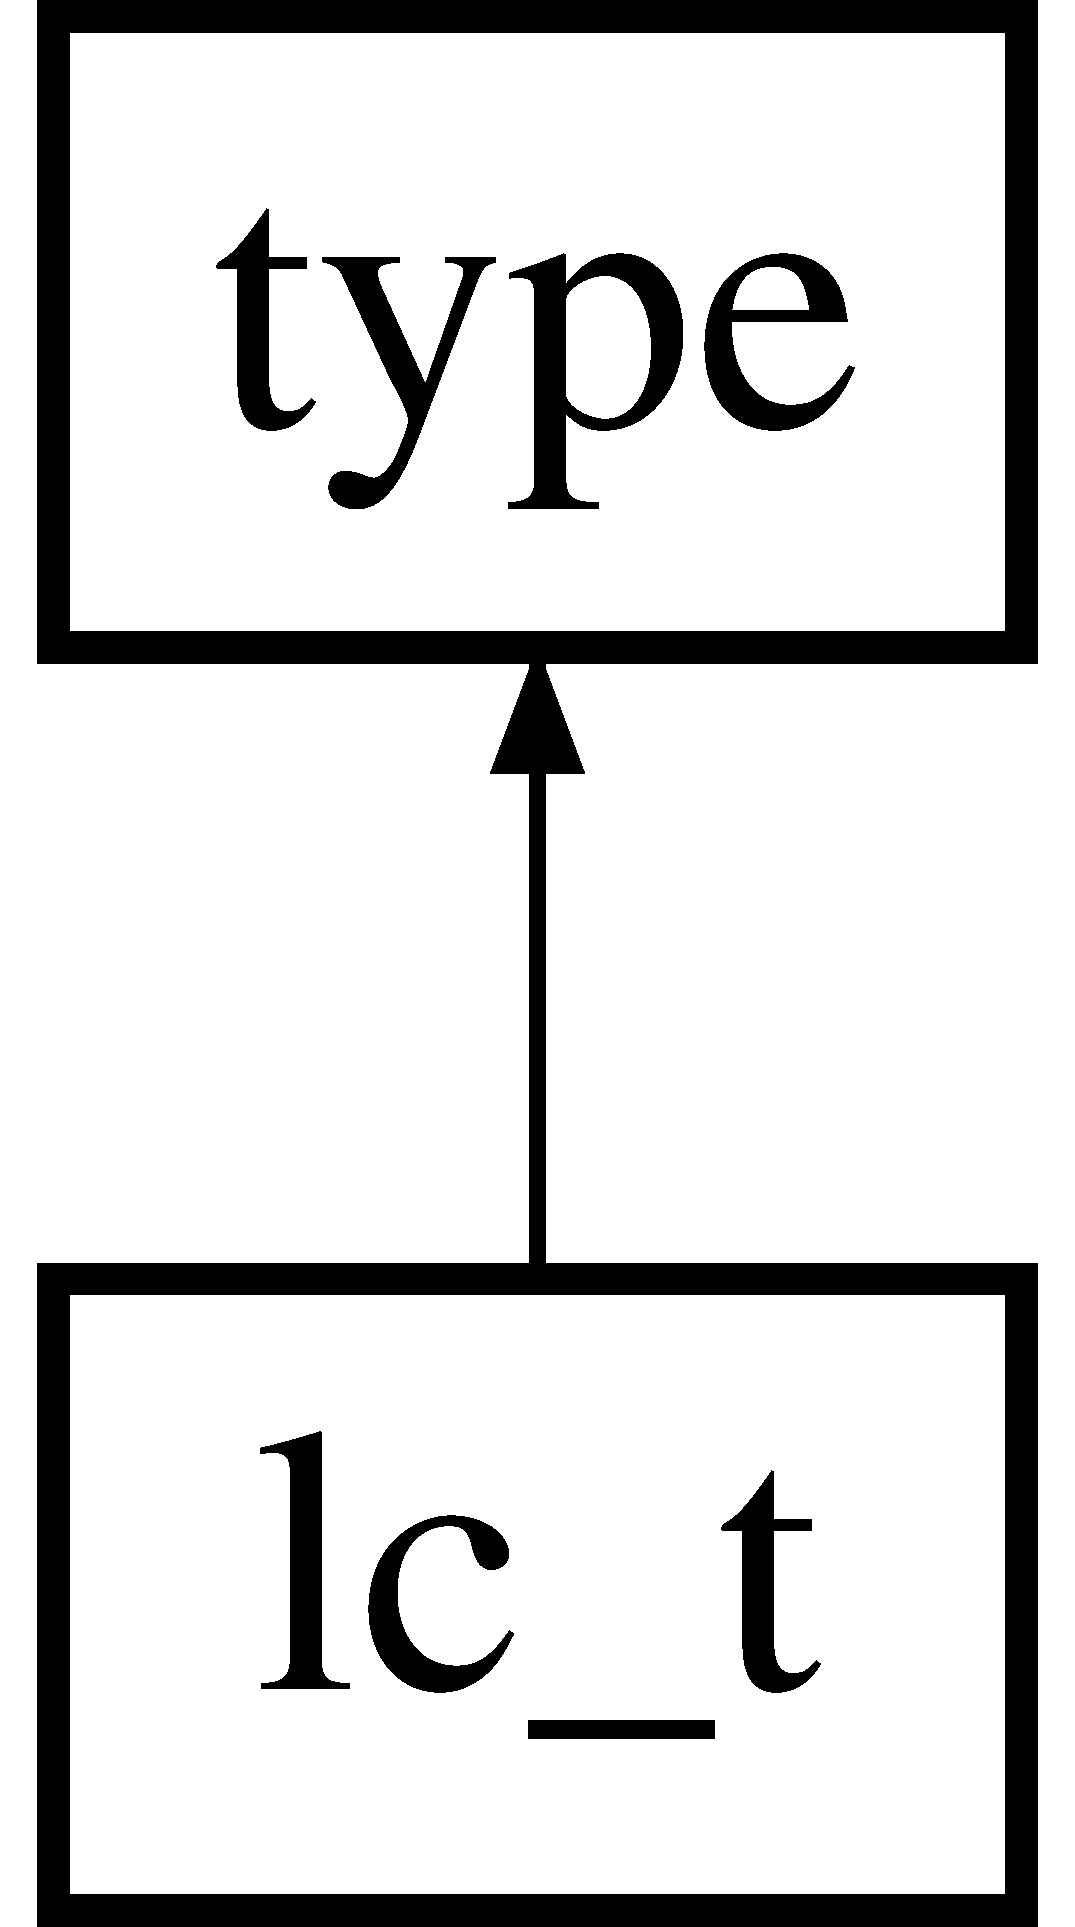
\includegraphics[height=2.000000cm]{classlc__t}
\end{center}
\end{figure}
\subsection*{Public Types}
\begin{DoxyCompactItemize}
\item 
typedef \-::\hyperlink{classdomainsize__t}{domainsize\-\_\-t} \hyperlink{classlc__t_a14e4ab30758da00bc9f186b0ef06a97e}{domainsize\-\_\-type}
\item 
typedef \\*
\-::xsd\-::cxx\-::tree\-::traits\\*
$<$ \hyperlink{classlc__t_a14e4ab30758da00bc9f186b0ef06a97e}{domainsize\-\_\-type}, char $>$ \hyperlink{classlc__t_af080ee9e8205b4e027f18eaa42a8bdfa}{domainsize\-\_\-traits}
\item 
typedef \-::\hyperlink{namespacexml__schema_a69bfaf24f63a8c18ebd8e21db6b343df}{xml\-\_\-schema\-::decimal} \hyperlink{classlc__t_aeee50e2ac6fe42996cb39a92ad78883e}{rcutoff\-\_\-type}
\item 
typedef \\*
\-::xsd\-::cxx\-::tree\-::traits\\*
$<$ \hyperlink{classlc__t_aeee50e2ac6fe42996cb39a92ad78883e}{rcutoff\-\_\-type}, char,\-::xsd\-::cxx\-::tree\-::schema\-\_\-type\-::decimal $>$ \hyperlink{classlc__t_a0e4c76efd7229ca57c957d12422c9ebc}{rcutoff\-\_\-traits}
\item 
typedef \-::\hyperlink{classcondition__t}{condition\-\_\-t} \hyperlink{classlc__t_aeb4f39b796939efd5541331610d5e28e}{condition\-\_\-type}
\item 
typedef \\*
\-::xsd\-::cxx\-::tree\-::sequence\\*
$<$ \hyperlink{classlc__t_aeb4f39b796939efd5541331610d5e28e}{condition\-\_\-type} $>$ \hyperlink{classlc__t_a0ee6b40c23baf2237388873de0c9df3f}{condition\-\_\-sequence}
\item 
typedef \\*
condition\-\_\-sequence\-::iterator \hyperlink{classlc__t_a2cd4737a0b7e2c244e6ec8ab87d99c1f}{condition\-\_\-iterator}
\item 
typedef \\*
condition\-\_\-sequence\-::const\-\_\-iterator \hyperlink{classlc__t_a8cd4fbfb140695f669c9ce89e8755f50}{condition\-\_\-const\-\_\-iterator}
\item 
typedef \\*
\-::xsd\-::cxx\-::tree\-::traits\\*
$<$ \hyperlink{classlc__t_aeb4f39b796939efd5541331610d5e28e}{condition\-\_\-type}, char $>$ \hyperlink{classlc__t_a484a730347d961f1270bdd8d61bbcda2}{condition\-\_\-traits}
\end{DoxyCompactItemize}
\subsection*{Public Member Functions}
\begin{DoxyCompactItemize}
\item 
const \hyperlink{classlc__t_a14e4ab30758da00bc9f186b0ef06a97e}{domainsize\-\_\-type} \& \hyperlink{classlc__t_ae7d80b95cc85ddd6a3461fac75cc3e5d}{domainsize} () const 
\item 
\hyperlink{classlc__t_a14e4ab30758da00bc9f186b0ef06a97e}{domainsize\-\_\-type} \& \hyperlink{classlc__t_a22daf97db73443148a86d81fdf071b46}{domainsize} ()
\item 
void \hyperlink{classlc__t_acdf9b3388324ce06b225a065a44cc693}{domainsize} (const \hyperlink{classlc__t_a14e4ab30758da00bc9f186b0ef06a97e}{domainsize\-\_\-type} \&x)
\item 
void \hyperlink{classlc__t_a58cb201bccba999cf88cd42a27ddb528}{domainsize} (\-::std\-::auto\-\_\-ptr$<$ \hyperlink{classlc__t_a14e4ab30758da00bc9f186b0ef06a97e}{domainsize\-\_\-type} $>$ p)
\item 
const \hyperlink{classlc__t_aeee50e2ac6fe42996cb39a92ad78883e}{rcutoff\-\_\-type} \& \hyperlink{classlc__t_a59976922c45ca81470b9766c08fe891e}{rcutoff} () const 
\item 
\hyperlink{classlc__t_aeee50e2ac6fe42996cb39a92ad78883e}{rcutoff\-\_\-type} \& \hyperlink{classlc__t_a646434eaec4a3ffeeedd40928eda2dfd}{rcutoff} ()
\item 
void \hyperlink{classlc__t_a36e418944e3409c2cafb07f115cf317a}{rcutoff} (const \hyperlink{classlc__t_aeee50e2ac6fe42996cb39a92ad78883e}{rcutoff\-\_\-type} \&x)
\item 
const \hyperlink{classlc__t_a0ee6b40c23baf2237388873de0c9df3f}{condition\-\_\-sequence} \& \hyperlink{classlc__t_a3ebe73f89c78475fc19ec459b40ed193}{condition} () const 
\item 
\hyperlink{classlc__t_a0ee6b40c23baf2237388873de0c9df3f}{condition\-\_\-sequence} \& \hyperlink{classlc__t_a7c7290f4578db48bba9b678a48083a61}{condition} ()
\item 
void \hyperlink{classlc__t_a03178f2b8c91b04faedcd0abd7df5aff}{condition} (const \hyperlink{classlc__t_a0ee6b40c23baf2237388873de0c9df3f}{condition\-\_\-sequence} \&s)
\item 
\hyperlink{classlc__t_ac66336f0d6a44cbe9f896ac9fd441aec}{lc\-\_\-t} (const \hyperlink{classlc__t_a14e4ab30758da00bc9f186b0ef06a97e}{domainsize\-\_\-type} \&, const \hyperlink{classlc__t_aeee50e2ac6fe42996cb39a92ad78883e}{rcutoff\-\_\-type} \&)
\item 
\hyperlink{classlc__t_a3b7b9d1fa28656ded4069a0177bf1297}{lc\-\_\-t} (\-::std\-::auto\-\_\-ptr$<$ \hyperlink{classlc__t_a14e4ab30758da00bc9f186b0ef06a97e}{domainsize\-\_\-type} $>$ \&, const \hyperlink{classlc__t_aeee50e2ac6fe42996cb39a92ad78883e}{rcutoff\-\_\-type} \&)
\item 
\hyperlink{classlc__t_afc944263c2450efa255b3b5669e62ba6}{lc\-\_\-t} (const \-::xercesc\-::\-D\-O\-M\-Element \&e,\-::\hyperlink{namespacexml__schema_a0612287d030cb2732d31a45b258fdc87}{xml\-\_\-schema\-::flags} f=0,\-::\hyperlink{namespacexml__schema_ada9aa30dc722e93ee2ed7243085402a5}{xml\-\_\-schema\-::container} $\ast$c=0)
\item 
\hyperlink{classlc__t_a87e7f3976afb8500ec97e69edd7cfac5}{lc\-\_\-t} (const \hyperlink{classlc__t}{lc\-\_\-t} \&x,\-::\hyperlink{namespacexml__schema_a0612287d030cb2732d31a45b258fdc87}{xml\-\_\-schema\-::flags} f=0,\-::\hyperlink{namespacexml__schema_ada9aa30dc722e93ee2ed7243085402a5}{xml\-\_\-schema\-::container} $\ast$c=0)
\item 
virtual \hyperlink{classlc__t}{lc\-\_\-t} $\ast$ \hyperlink{classlc__t_af8d3a68bf8d7ba42ef03c24439bbfb63}{\-\_\-clone} (\-::\hyperlink{namespacexml__schema_a0612287d030cb2732d31a45b258fdc87}{xml\-\_\-schema\-::flags} f=0,\-::\hyperlink{namespacexml__schema_ada9aa30dc722e93ee2ed7243085402a5}{xml\-\_\-schema\-::container} $\ast$c=0) const 
\item 
virtual \hyperlink{classlc__t_a40d77173a6b92f269bc4445453919fc1}{$\sim$lc\-\_\-t} ()
\end{DoxyCompactItemize}
\subsection*{Protected Member Functions}
\begin{DoxyCompactItemize}
\item 
void \hyperlink{classlc__t_a805dd25d448f39324c1b262930fe15d2}{parse} (\-::xsd\-::cxx\-::xml\-::dom\-::parser$<$ char $>$ \&,\-::\hyperlink{namespacexml__schema_a0612287d030cb2732d31a45b258fdc87}{xml\-\_\-schema\-::flags})
\end{DoxyCompactItemize}
\subsection*{Protected Attributes}
\begin{DoxyCompactItemize}
\item 
\-::xsd\-::cxx\-::tree\-::one\\*
$<$ \hyperlink{classlc__t_a14e4ab30758da00bc9f186b0ef06a97e}{domainsize\-\_\-type} $>$ \hyperlink{classlc__t_a55f74434096a0a3a65a7b6e1cc7896e1}{domainsize\-\_\-}
\item 
\-::xsd\-::cxx\-::tree\-::one\\*
$<$ \hyperlink{classlc__t_aeee50e2ac6fe42996cb39a92ad78883e}{rcutoff\-\_\-type} $>$ \hyperlink{classlc__t_a55af0ea7d58424b078f479cfa7465205}{rcutoff\-\_\-}
\item 
\hyperlink{classlc__t_a0ee6b40c23baf2237388873de0c9df3f}{condition\-\_\-sequence} \hyperlink{classlc__t_a8f977c09da602f2414c759e261795ba8}{condition\-\_\-}
\end{DoxyCompactItemize}


\subsection{Member Typedef Documentation}
\hypertarget{classlc__t_a8cd4fbfb140695f669c9ce89e8755f50}{\index{lc\-\_\-t@{lc\-\_\-t}!condition\-\_\-const\-\_\-iterator@{condition\-\_\-const\-\_\-iterator}}
\index{condition\-\_\-const\-\_\-iterator@{condition\-\_\-const\-\_\-iterator}!lc_t@{lc\-\_\-t}}
\subsubsection[{condition\-\_\-const\-\_\-iterator}]{\setlength{\rightskip}{0pt plus 5cm}typedef condition\-\_\-sequence\-::const\-\_\-iterator {\bf lc\-\_\-t\-::condition\-\_\-const\-\_\-iterator}}}\label{classlc__t_a8cd4fbfb140695f669c9ce89e8755f50}
\hypertarget{classlc__t_a2cd4737a0b7e2c244e6ec8ab87d99c1f}{\index{lc\-\_\-t@{lc\-\_\-t}!condition\-\_\-iterator@{condition\-\_\-iterator}}
\index{condition\-\_\-iterator@{condition\-\_\-iterator}!lc_t@{lc\-\_\-t}}
\subsubsection[{condition\-\_\-iterator}]{\setlength{\rightskip}{0pt plus 5cm}typedef condition\-\_\-sequence\-::iterator {\bf lc\-\_\-t\-::condition\-\_\-iterator}}}\label{classlc__t_a2cd4737a0b7e2c244e6ec8ab87d99c1f}
\hypertarget{classlc__t_a0ee6b40c23baf2237388873de0c9df3f}{\index{lc\-\_\-t@{lc\-\_\-t}!condition\-\_\-sequence@{condition\-\_\-sequence}}
\index{condition\-\_\-sequence@{condition\-\_\-sequence}!lc_t@{lc\-\_\-t}}
\subsubsection[{condition\-\_\-sequence}]{\setlength{\rightskip}{0pt plus 5cm}typedef \-::xsd\-::cxx\-::tree\-::sequence$<$ {\bf condition\-\_\-type} $>$ {\bf lc\-\_\-t\-::condition\-\_\-sequence}}}\label{classlc__t_a0ee6b40c23baf2237388873de0c9df3f}
\hypertarget{classlc__t_a484a730347d961f1270bdd8d61bbcda2}{\index{lc\-\_\-t@{lc\-\_\-t}!condition\-\_\-traits@{condition\-\_\-traits}}
\index{condition\-\_\-traits@{condition\-\_\-traits}!lc_t@{lc\-\_\-t}}
\subsubsection[{condition\-\_\-traits}]{\setlength{\rightskip}{0pt plus 5cm}typedef \-::xsd\-::cxx\-::tree\-::traits$<$ {\bf condition\-\_\-type}, char $>$ {\bf lc\-\_\-t\-::condition\-\_\-traits}}}\label{classlc__t_a484a730347d961f1270bdd8d61bbcda2}
\hypertarget{classlc__t_aeb4f39b796939efd5541331610d5e28e}{\index{lc\-\_\-t@{lc\-\_\-t}!condition\-\_\-type@{condition\-\_\-type}}
\index{condition\-\_\-type@{condition\-\_\-type}!lc_t@{lc\-\_\-t}}
\subsubsection[{condition\-\_\-type}]{\setlength{\rightskip}{0pt plus 5cm}typedef \-::{\bf condition\-\_\-t} {\bf lc\-\_\-t\-::condition\-\_\-type}}}\label{classlc__t_aeb4f39b796939efd5541331610d5e28e}
\hypertarget{classlc__t_af080ee9e8205b4e027f18eaa42a8bdfa}{\index{lc\-\_\-t@{lc\-\_\-t}!domainsize\-\_\-traits@{domainsize\-\_\-traits}}
\index{domainsize\-\_\-traits@{domainsize\-\_\-traits}!lc_t@{lc\-\_\-t}}
\subsubsection[{domainsize\-\_\-traits}]{\setlength{\rightskip}{0pt plus 5cm}typedef \-::xsd\-::cxx\-::tree\-::traits$<$ {\bf domainsize\-\_\-type}, char $>$ {\bf lc\-\_\-t\-::domainsize\-\_\-traits}}}\label{classlc__t_af080ee9e8205b4e027f18eaa42a8bdfa}
\hypertarget{classlc__t_a14e4ab30758da00bc9f186b0ef06a97e}{\index{lc\-\_\-t@{lc\-\_\-t}!domainsize\-\_\-type@{domainsize\-\_\-type}}
\index{domainsize\-\_\-type@{domainsize\-\_\-type}!lc_t@{lc\-\_\-t}}
\subsubsection[{domainsize\-\_\-type}]{\setlength{\rightskip}{0pt plus 5cm}typedef \-::{\bf domainsize\-\_\-t} {\bf lc\-\_\-t\-::domainsize\-\_\-type}}}\label{classlc__t_a14e4ab30758da00bc9f186b0ef06a97e}
\hypertarget{classlc__t_a0e4c76efd7229ca57c957d12422c9ebc}{\index{lc\-\_\-t@{lc\-\_\-t}!rcutoff\-\_\-traits@{rcutoff\-\_\-traits}}
\index{rcutoff\-\_\-traits@{rcutoff\-\_\-traits}!lc_t@{lc\-\_\-t}}
\subsubsection[{rcutoff\-\_\-traits}]{\setlength{\rightskip}{0pt plus 5cm}typedef \-::xsd\-::cxx\-::tree\-::traits$<$ {\bf rcutoff\-\_\-type}, char, \-::xsd\-::cxx\-::tree\-::schema\-\_\-type\-::decimal $>$ {\bf lc\-\_\-t\-::rcutoff\-\_\-traits}}}\label{classlc__t_a0e4c76efd7229ca57c957d12422c9ebc}
\hypertarget{classlc__t_aeee50e2ac6fe42996cb39a92ad78883e}{\index{lc\-\_\-t@{lc\-\_\-t}!rcutoff\-\_\-type@{rcutoff\-\_\-type}}
\index{rcutoff\-\_\-type@{rcutoff\-\_\-type}!lc_t@{lc\-\_\-t}}
\subsubsection[{rcutoff\-\_\-type}]{\setlength{\rightskip}{0pt plus 5cm}typedef \-::{\bf xml\-\_\-schema\-::decimal} {\bf lc\-\_\-t\-::rcutoff\-\_\-type}}}\label{classlc__t_aeee50e2ac6fe42996cb39a92ad78883e}


\subsection{Constructor \& Destructor Documentation}
\hypertarget{classlc__t_ac66336f0d6a44cbe9f896ac9fd441aec}{\index{lc\-\_\-t@{lc\-\_\-t}!lc\-\_\-t@{lc\-\_\-t}}
\index{lc\-\_\-t@{lc\-\_\-t}!lc_t@{lc\-\_\-t}}
\subsubsection[{lc\-\_\-t}]{\setlength{\rightskip}{0pt plus 5cm}lc\-\_\-t\-::lc\-\_\-t (
\begin{DoxyParamCaption}
\item[{const {\bf domainsize\-\_\-type} \&}]{domainsize, }
\item[{const {\bf rcutoff\-\_\-type} \&}]{rcutoff}
\end{DoxyParamCaption}
)}}\label{classlc__t_ac66336f0d6a44cbe9f896ac9fd441aec}
\hypertarget{classlc__t_a3b7b9d1fa28656ded4069a0177bf1297}{\index{lc\-\_\-t@{lc\-\_\-t}!lc\-\_\-t@{lc\-\_\-t}}
\index{lc\-\_\-t@{lc\-\_\-t}!lc_t@{lc\-\_\-t}}
\subsubsection[{lc\-\_\-t}]{\setlength{\rightskip}{0pt plus 5cm}lc\-\_\-t\-::lc\-\_\-t (
\begin{DoxyParamCaption}
\item[{\-::std\-::auto\-\_\-ptr$<$ {\bf domainsize\-\_\-type} $>$ \&}]{domainsize, }
\item[{const {\bf rcutoff\-\_\-type} \&}]{rcutoff}
\end{DoxyParamCaption}
)}}\label{classlc__t_a3b7b9d1fa28656ded4069a0177bf1297}
\hypertarget{classlc__t_afc944263c2450efa255b3b5669e62ba6}{\index{lc\-\_\-t@{lc\-\_\-t}!lc\-\_\-t@{lc\-\_\-t}}
\index{lc\-\_\-t@{lc\-\_\-t}!lc_t@{lc\-\_\-t}}
\subsubsection[{lc\-\_\-t}]{\setlength{\rightskip}{0pt plus 5cm}lc\-\_\-t\-::lc\-\_\-t (
\begin{DoxyParamCaption}
\item[{const \-::xercesc\-::\-D\-O\-M\-Element \&}]{e, }
\item[{\-::{\bf xml\-\_\-schema\-::flags}}]{f = {\ttfamily 0}, }
\item[{\-::{\bf xml\-\_\-schema\-::container} $\ast$}]{c = {\ttfamily 0}}
\end{DoxyParamCaption}
)}}\label{classlc__t_afc944263c2450efa255b3b5669e62ba6}
\hypertarget{classlc__t_a87e7f3976afb8500ec97e69edd7cfac5}{\index{lc\-\_\-t@{lc\-\_\-t}!lc\-\_\-t@{lc\-\_\-t}}
\index{lc\-\_\-t@{lc\-\_\-t}!lc_t@{lc\-\_\-t}}
\subsubsection[{lc\-\_\-t}]{\setlength{\rightskip}{0pt plus 5cm}lc\-\_\-t\-::lc\-\_\-t (
\begin{DoxyParamCaption}
\item[{const {\bf lc\-\_\-t} \&}]{x, }
\item[{\-::{\bf xml\-\_\-schema\-::flags}}]{f = {\ttfamily 0}, }
\item[{\-::{\bf xml\-\_\-schema\-::container} $\ast$}]{c = {\ttfamily 0}}
\end{DoxyParamCaption}
)}}\label{classlc__t_a87e7f3976afb8500ec97e69edd7cfac5}
\hypertarget{classlc__t_a40d77173a6b92f269bc4445453919fc1}{\index{lc\-\_\-t@{lc\-\_\-t}!$\sim$lc\-\_\-t@{$\sim$lc\-\_\-t}}
\index{$\sim$lc\-\_\-t@{$\sim$lc\-\_\-t}!lc_t@{lc\-\_\-t}}
\subsubsection[{$\sim$lc\-\_\-t}]{\setlength{\rightskip}{0pt plus 5cm}lc\-\_\-t\-::$\sim$lc\-\_\-t (
\begin{DoxyParamCaption}
{}
\end{DoxyParamCaption}
)\hspace{0.3cm}{\ttfamily [virtual]}}}\label{classlc__t_a40d77173a6b92f269bc4445453919fc1}


\subsection{Member Function Documentation}
\hypertarget{classlc__t_af8d3a68bf8d7ba42ef03c24439bbfb63}{\index{lc\-\_\-t@{lc\-\_\-t}!\-\_\-clone@{\-\_\-clone}}
\index{\-\_\-clone@{\-\_\-clone}!lc_t@{lc\-\_\-t}}
\subsubsection[{\-\_\-clone}]{\setlength{\rightskip}{0pt plus 5cm}{\bf lc\-\_\-t} $\ast$ lc\-\_\-t\-::\-\_\-clone (
\begin{DoxyParamCaption}
\item[{\-::{\bf xml\-\_\-schema\-::flags}}]{f = {\ttfamily 0}, }
\item[{\-::{\bf xml\-\_\-schema\-::container} $\ast$}]{c = {\ttfamily 0}}
\end{DoxyParamCaption}
) const\hspace{0.3cm}{\ttfamily [virtual]}}}\label{classlc__t_af8d3a68bf8d7ba42ef03c24439bbfb63}
\hypertarget{classlc__t_a3ebe73f89c78475fc19ec459b40ed193}{\index{lc\-\_\-t@{lc\-\_\-t}!condition@{condition}}
\index{condition@{condition}!lc_t@{lc\-\_\-t}}
\subsubsection[{condition}]{\setlength{\rightskip}{0pt plus 5cm}const {\bf lc\-\_\-t\-::condition\-\_\-sequence} \& lc\-\_\-t\-::condition (
\begin{DoxyParamCaption}
{}
\end{DoxyParamCaption}
) const}}\label{classlc__t_a3ebe73f89c78475fc19ec459b40ed193}
\hypertarget{classlc__t_a7c7290f4578db48bba9b678a48083a61}{\index{lc\-\_\-t@{lc\-\_\-t}!condition@{condition}}
\index{condition@{condition}!lc_t@{lc\-\_\-t}}
\subsubsection[{condition}]{\setlength{\rightskip}{0pt plus 5cm}{\bf lc\-\_\-t\-::condition\-\_\-sequence} \& lc\-\_\-t\-::condition (
\begin{DoxyParamCaption}
{}
\end{DoxyParamCaption}
)}}\label{classlc__t_a7c7290f4578db48bba9b678a48083a61}
\hypertarget{classlc__t_a03178f2b8c91b04faedcd0abd7df5aff}{\index{lc\-\_\-t@{lc\-\_\-t}!condition@{condition}}
\index{condition@{condition}!lc_t@{lc\-\_\-t}}
\subsubsection[{condition}]{\setlength{\rightskip}{0pt plus 5cm}void lc\-\_\-t\-::condition (
\begin{DoxyParamCaption}
\item[{const {\bf condition\-\_\-sequence} \&}]{s}
\end{DoxyParamCaption}
)}}\label{classlc__t_a03178f2b8c91b04faedcd0abd7df5aff}
\hypertarget{classlc__t_ae7d80b95cc85ddd6a3461fac75cc3e5d}{\index{lc\-\_\-t@{lc\-\_\-t}!domainsize@{domainsize}}
\index{domainsize@{domainsize}!lc_t@{lc\-\_\-t}}
\subsubsection[{domainsize}]{\setlength{\rightskip}{0pt plus 5cm}const {\bf lc\-\_\-t\-::domainsize\-\_\-type} \& lc\-\_\-t\-::domainsize (
\begin{DoxyParamCaption}
{}
\end{DoxyParamCaption}
) const}}\label{classlc__t_ae7d80b95cc85ddd6a3461fac75cc3e5d}
\hypertarget{classlc__t_a22daf97db73443148a86d81fdf071b46}{\index{lc\-\_\-t@{lc\-\_\-t}!domainsize@{domainsize}}
\index{domainsize@{domainsize}!lc_t@{lc\-\_\-t}}
\subsubsection[{domainsize}]{\setlength{\rightskip}{0pt plus 5cm}{\bf lc\-\_\-t\-::domainsize\-\_\-type} \& lc\-\_\-t\-::domainsize (
\begin{DoxyParamCaption}
{}
\end{DoxyParamCaption}
)}}\label{classlc__t_a22daf97db73443148a86d81fdf071b46}
\hypertarget{classlc__t_acdf9b3388324ce06b225a065a44cc693}{\index{lc\-\_\-t@{lc\-\_\-t}!domainsize@{domainsize}}
\index{domainsize@{domainsize}!lc_t@{lc\-\_\-t}}
\subsubsection[{domainsize}]{\setlength{\rightskip}{0pt plus 5cm}void lc\-\_\-t\-::domainsize (
\begin{DoxyParamCaption}
\item[{const {\bf domainsize\-\_\-type} \&}]{x}
\end{DoxyParamCaption}
)}}\label{classlc__t_acdf9b3388324ce06b225a065a44cc693}
\hypertarget{classlc__t_a58cb201bccba999cf88cd42a27ddb528}{\index{lc\-\_\-t@{lc\-\_\-t}!domainsize@{domainsize}}
\index{domainsize@{domainsize}!lc_t@{lc\-\_\-t}}
\subsubsection[{domainsize}]{\setlength{\rightskip}{0pt plus 5cm}void lc\-\_\-t\-::domainsize (
\begin{DoxyParamCaption}
\item[{\-::std\-::auto\-\_\-ptr$<$ {\bf domainsize\-\_\-type} $>$}]{p}
\end{DoxyParamCaption}
)}}\label{classlc__t_a58cb201bccba999cf88cd42a27ddb528}
\hypertarget{classlc__t_a805dd25d448f39324c1b262930fe15d2}{\index{lc\-\_\-t@{lc\-\_\-t}!parse@{parse}}
\index{parse@{parse}!lc_t@{lc\-\_\-t}}
\subsubsection[{parse}]{\setlength{\rightskip}{0pt plus 5cm}void lc\-\_\-t\-::parse (
\begin{DoxyParamCaption}
\item[{\-::xsd\-::cxx\-::xml\-::dom\-::parser$<$ char $>$ \&}]{p, }
\item[{\-::{\bf xml\-\_\-schema\-::flags}}]{f}
\end{DoxyParamCaption}
)\hspace{0.3cm}{\ttfamily [protected]}}}\label{classlc__t_a805dd25d448f39324c1b262930fe15d2}
\hypertarget{classlc__t_a59976922c45ca81470b9766c08fe891e}{\index{lc\-\_\-t@{lc\-\_\-t}!rcutoff@{rcutoff}}
\index{rcutoff@{rcutoff}!lc_t@{lc\-\_\-t}}
\subsubsection[{rcutoff}]{\setlength{\rightskip}{0pt plus 5cm}const {\bf lc\-\_\-t\-::rcutoff\-\_\-type} \& lc\-\_\-t\-::rcutoff (
\begin{DoxyParamCaption}
{}
\end{DoxyParamCaption}
) const}}\label{classlc__t_a59976922c45ca81470b9766c08fe891e}
\hypertarget{classlc__t_a646434eaec4a3ffeeedd40928eda2dfd}{\index{lc\-\_\-t@{lc\-\_\-t}!rcutoff@{rcutoff}}
\index{rcutoff@{rcutoff}!lc_t@{lc\-\_\-t}}
\subsubsection[{rcutoff}]{\setlength{\rightskip}{0pt plus 5cm}{\bf lc\-\_\-t\-::rcutoff\-\_\-type} \& lc\-\_\-t\-::rcutoff (
\begin{DoxyParamCaption}
{}
\end{DoxyParamCaption}
)}}\label{classlc__t_a646434eaec4a3ffeeedd40928eda2dfd}
\hypertarget{classlc__t_a36e418944e3409c2cafb07f115cf317a}{\index{lc\-\_\-t@{lc\-\_\-t}!rcutoff@{rcutoff}}
\index{rcutoff@{rcutoff}!lc_t@{lc\-\_\-t}}
\subsubsection[{rcutoff}]{\setlength{\rightskip}{0pt plus 5cm}void lc\-\_\-t\-::rcutoff (
\begin{DoxyParamCaption}
\item[{const {\bf rcutoff\-\_\-type} \&}]{x}
\end{DoxyParamCaption}
)}}\label{classlc__t_a36e418944e3409c2cafb07f115cf317a}


\subsection{Member Data Documentation}
\hypertarget{classlc__t_a8f977c09da602f2414c759e261795ba8}{\index{lc\-\_\-t@{lc\-\_\-t}!condition\-\_\-@{condition\-\_\-}}
\index{condition\-\_\-@{condition\-\_\-}!lc_t@{lc\-\_\-t}}
\subsubsection[{condition\-\_\-}]{\setlength{\rightskip}{0pt plus 5cm}{\bf condition\-\_\-sequence} lc\-\_\-t\-::condition\-\_\-\hspace{0.3cm}{\ttfamily [protected]}}}\label{classlc__t_a8f977c09da602f2414c759e261795ba8}
\hypertarget{classlc__t_a55f74434096a0a3a65a7b6e1cc7896e1}{\index{lc\-\_\-t@{lc\-\_\-t}!domainsize\-\_\-@{domainsize\-\_\-}}
\index{domainsize\-\_\-@{domainsize\-\_\-}!lc_t@{lc\-\_\-t}}
\subsubsection[{domainsize\-\_\-}]{\setlength{\rightskip}{0pt plus 5cm}\-::xsd\-::cxx\-::tree\-::one$<$ {\bf domainsize\-\_\-type} $>$ lc\-\_\-t\-::domainsize\-\_\-\hspace{0.3cm}{\ttfamily [protected]}}}\label{classlc__t_a55f74434096a0a3a65a7b6e1cc7896e1}
\hypertarget{classlc__t_a55af0ea7d58424b078f479cfa7465205}{\index{lc\-\_\-t@{lc\-\_\-t}!rcutoff\-\_\-@{rcutoff\-\_\-}}
\index{rcutoff\-\_\-@{rcutoff\-\_\-}!lc_t@{lc\-\_\-t}}
\subsubsection[{rcutoff\-\_\-}]{\setlength{\rightskip}{0pt plus 5cm}\-::xsd\-::cxx\-::tree\-::one$<$ {\bf rcutoff\-\_\-type} $>$ lc\-\_\-t\-::rcutoff\-\_\-\hspace{0.3cm}{\ttfamily [protected]}}}\label{classlc__t_a55af0ea7d58424b078f479cfa7465205}


The documentation for this class was generated from the following files\-:\begin{DoxyCompactItemize}
\item 
src/utils/\hyperlink{InputSetting_8h}{Input\-Setting.\-h}\item 
src/utils/\hyperlink{InputSetting_8cpp}{Input\-Setting.\-cpp}\end{DoxyCompactItemize}

\hypertarget{classutils_1_1LCInnerParticleIterator}{\section{utils\-:\-:L\-C\-Inner\-Particle\-Iterator Class Reference}
\label{classutils_1_1LCInnerParticleIterator}\index{utils\-::\-L\-C\-Inner\-Particle\-Iterator@{utils\-::\-L\-C\-Inner\-Particle\-Iterator}}
}


{\ttfamily \#include $<$L\-C\-Inner\-Particle\-Iterator.\-h$>$}

\subsection*{Public Member Functions}
\begin{DoxyCompactItemize}
\item 
\hyperlink{classutils_1_1LCInnerParticleIterator_a97ed0538282db641bccd20e2700c1b49}{L\-C\-Inner\-Particle\-Iterator} ()
\item 
\hyperlink{classutils_1_1LCInnerParticleIterator_aad380c74a45caefe96d125ccb02b7ecf}{L\-C\-Inner\-Particle\-Iterator} (int index\-\_\-arg, int original\-\_\-index\-\_\-arg, int cell\-\_\-size\-\_\-arg, int width\-\_\-arg, int height\-\_\-arg, int depth\-\_\-arg, std\-::list$<$ \hyperlink{classParticle}{Particle} $\ast$ $>$\-::\hyperlink{classutils_1_1LCInnerParticleIterator_a556926724858f489ff82ba151748bd4d}{iterator} iterator\-\_\-arg, std\-::vector$<$ std\-::list$<$ \hyperlink{classParticle}{Particle} $\ast$ $>$ $\ast$ $>$ $\ast$cells\-\_\-arg)
\item 
virtual \hyperlink{classutils_1_1LCInnerParticleIterator_aeb7069368fc24e7c765348aa2b9cefc9}{$\sim$\-L\-C\-Inner\-Particle\-Iterator} ()
\item 
\hyperlink{classParticle}{Particle} \& \hyperlink{classutils_1_1LCInnerParticleIterator_a3b1af69d0bfe72d9e2c3d59f8735d765}{operator$\ast$} () const 
\item 
void \hyperlink{classutils_1_1LCInnerParticleIterator_a617483a82dcbc3e47da991a6c1c628df}{operator++} ()
\item 
bool \hyperlink{classutils_1_1LCInnerParticleIterator_ac924555155c3d389612b8cf2ed1ce7af}{operator!=} (const \hyperlink{classutils_1_1LCInnerParticleIterator}{L\-C\-Inner\-Particle\-Iterator} b)
\item 
\hyperlink{classutils_1_1LCInnerParticleIterator}{L\-C\-Inner\-Particle\-Iterator} \& \hyperlink{classutils_1_1LCInnerParticleIterator_a23019e15648c8aff3f4f210d09bd3e1d}{operator=} (const \hyperlink{classutils_1_1LCInnerParticleIterator}{L\-C\-Inner\-Particle\-Iterator} \&cpy)
\item 
int \hyperlink{classutils_1_1LCInnerParticleIterator_aac709e0bd8324335cf5e261abcc462d5}{get\-Cell\-Number} ()
\item 
bool \hyperlink{classutils_1_1LCInnerParticleIterator_a3351f46c7b9cc23b8c7cfaed21a3ab21}{check\-Left} ()
\item 
bool \hyperlink{classutils_1_1LCInnerParticleIterator_a9b7095262c5822b79f2fe5b9c864bc5c}{check\-Right} ()
\item 
bool \hyperlink{classutils_1_1LCInnerParticleIterator_ac0a650efc58403e2acbf191ee25f99d5}{check\-Bottom} ()
\item 
bool \hyperlink{classutils_1_1LCInnerParticleIterator_af014915da19b22640850eb676b8e0ab0}{check\-Back} ()
\item 
bool \hyperlink{classutils_1_1LCInnerParticleIterator_a079d0a446521b35730ca4f3d6204f5e7}{check\-Top} ()
\end{DoxyCompactItemize}
\subsection*{Private Attributes}
\begin{DoxyCompactItemize}
\item 
std\-::vector$<$ std\-::list\\*
$<$ \hyperlink{classParticle}{Particle} $\ast$ $>$ $\ast$ $>$ $\ast$ \hyperlink{classutils_1_1LCInnerParticleIterator_a421358a111515986b506391956873ca8}{cells}
\item 
int \hyperlink{classutils_1_1LCInnerParticleIterator_a12d1e7f0dcc83d5ec4e09819b9e8f083}{cell\-\_\-size}
\item 
int \hyperlink{classutils_1_1LCInnerParticleIterator_a84770d6e782309bfc11ba2f965cb8f5c}{width}
\item 
int \hyperlink{classutils_1_1LCInnerParticleIterator_a1c2df47ebcba8c8c3d75ae2b7a136d7c}{height}
\item 
int \hyperlink{classutils_1_1LCInnerParticleIterator_a2a6d53e94efa6547736f66a6b0713c29}{depth}
\item 
int \hyperlink{classutils_1_1LCInnerParticleIterator_a27c807948fc9bfd2a30c94847530c39a}{index}
\item 
int \hyperlink{classutils_1_1LCInnerParticleIterator_a78f4884749444bd1ee25d874167dd582}{original\-\_\-index}
\item 
std\-::list$<$ \hyperlink{classParticle}{Particle} $\ast$ $>$\-::iterator \hyperlink{classutils_1_1LCInnerParticleIterator_a556926724858f489ff82ba151748bd4d}{iterator}
\end{DoxyCompactItemize}


\subsection{Constructor \& Destructor Documentation}
\hypertarget{classutils_1_1LCInnerParticleIterator_a97ed0538282db641bccd20e2700c1b49}{\index{utils\-::\-L\-C\-Inner\-Particle\-Iterator@{utils\-::\-L\-C\-Inner\-Particle\-Iterator}!L\-C\-Inner\-Particle\-Iterator@{L\-C\-Inner\-Particle\-Iterator}}
\index{L\-C\-Inner\-Particle\-Iterator@{L\-C\-Inner\-Particle\-Iterator}!utils::LCInnerParticleIterator@{utils\-::\-L\-C\-Inner\-Particle\-Iterator}}
\subsubsection[{L\-C\-Inner\-Particle\-Iterator}]{\setlength{\rightskip}{0pt plus 5cm}utils\-::\-L\-C\-Inner\-Particle\-Iterator\-::\-L\-C\-Inner\-Particle\-Iterator (
\begin{DoxyParamCaption}
{}
\end{DoxyParamCaption}
)}}\label{classutils_1_1LCInnerParticleIterator_a97ed0538282db641bccd20e2700c1b49}
\hypertarget{classutils_1_1LCInnerParticleIterator_aad380c74a45caefe96d125ccb02b7ecf}{\index{utils\-::\-L\-C\-Inner\-Particle\-Iterator@{utils\-::\-L\-C\-Inner\-Particle\-Iterator}!L\-C\-Inner\-Particle\-Iterator@{L\-C\-Inner\-Particle\-Iterator}}
\index{L\-C\-Inner\-Particle\-Iterator@{L\-C\-Inner\-Particle\-Iterator}!utils::LCInnerParticleIterator@{utils\-::\-L\-C\-Inner\-Particle\-Iterator}}
\subsubsection[{L\-C\-Inner\-Particle\-Iterator}]{\setlength{\rightskip}{0pt plus 5cm}utils\-::\-L\-C\-Inner\-Particle\-Iterator\-::\-L\-C\-Inner\-Particle\-Iterator (
\begin{DoxyParamCaption}
\item[{int}]{index\-\_\-arg, }
\item[{int}]{original\-\_\-index\-\_\-arg, }
\item[{int}]{cell\-\_\-size\-\_\-arg, }
\item[{int}]{width\-\_\-arg, }
\item[{int}]{height\-\_\-arg, }
\item[{int}]{depth\-\_\-arg, }
\item[{std\-::list$<$ {\bf Particle} $\ast$ $>$\-::{\bf iterator}}]{iterator\-\_\-arg, }
\item[{std\-::vector$<$ std\-::list$<$ {\bf Particle} $\ast$ $>$ $\ast$ $>$ $\ast$}]{cells\-\_\-arg}
\end{DoxyParamCaption}
)}}\label{classutils_1_1LCInnerParticleIterator_aad380c74a45caefe96d125ccb02b7ecf}
\hypertarget{classutils_1_1LCInnerParticleIterator_aeb7069368fc24e7c765348aa2b9cefc9}{\index{utils\-::\-L\-C\-Inner\-Particle\-Iterator@{utils\-::\-L\-C\-Inner\-Particle\-Iterator}!$\sim$\-L\-C\-Inner\-Particle\-Iterator@{$\sim$\-L\-C\-Inner\-Particle\-Iterator}}
\index{$\sim$\-L\-C\-Inner\-Particle\-Iterator@{$\sim$\-L\-C\-Inner\-Particle\-Iterator}!utils::LCInnerParticleIterator@{utils\-::\-L\-C\-Inner\-Particle\-Iterator}}
\subsubsection[{$\sim$\-L\-C\-Inner\-Particle\-Iterator}]{\setlength{\rightskip}{0pt plus 5cm}utils\-::\-L\-C\-Inner\-Particle\-Iterator\-::$\sim$\-L\-C\-Inner\-Particle\-Iterator (
\begin{DoxyParamCaption}
{}
\end{DoxyParamCaption}
)\hspace{0.3cm}{\ttfamily [virtual]}}}\label{classutils_1_1LCInnerParticleIterator_aeb7069368fc24e7c765348aa2b9cefc9}


\subsection{Member Function Documentation}
\hypertarget{classutils_1_1LCInnerParticleIterator_af014915da19b22640850eb676b8e0ab0}{\index{utils\-::\-L\-C\-Inner\-Particle\-Iterator@{utils\-::\-L\-C\-Inner\-Particle\-Iterator}!check\-Back@{check\-Back}}
\index{check\-Back@{check\-Back}!utils::LCInnerParticleIterator@{utils\-::\-L\-C\-Inner\-Particle\-Iterator}}
\subsubsection[{check\-Back}]{\setlength{\rightskip}{0pt plus 5cm}bool utils\-::\-L\-C\-Inner\-Particle\-Iterator\-::check\-Back (
\begin{DoxyParamCaption}
{}
\end{DoxyParamCaption}
)}}\label{classutils_1_1LCInnerParticleIterator_af014915da19b22640850eb676b8e0ab0}
checks whether the inner iterator may go to a deeper layer \hypertarget{classutils_1_1LCInnerParticleIterator_ac0a650efc58403e2acbf191ee25f99d5}{\index{utils\-::\-L\-C\-Inner\-Particle\-Iterator@{utils\-::\-L\-C\-Inner\-Particle\-Iterator}!check\-Bottom@{check\-Bottom}}
\index{check\-Bottom@{check\-Bottom}!utils::LCInnerParticleIterator@{utils\-::\-L\-C\-Inner\-Particle\-Iterator}}
\subsubsection[{check\-Bottom}]{\setlength{\rightskip}{0pt plus 5cm}bool utils\-::\-L\-C\-Inner\-Particle\-Iterator\-::check\-Bottom (
\begin{DoxyParamCaption}
{}
\end{DoxyParamCaption}
)}}\label{classutils_1_1LCInnerParticleIterator_ac0a650efc58403e2acbf191ee25f99d5}
checks whether the inner iterator may go to a lower layer \hypertarget{classutils_1_1LCInnerParticleIterator_a3351f46c7b9cc23b8c7cfaed21a3ab21}{\index{utils\-::\-L\-C\-Inner\-Particle\-Iterator@{utils\-::\-L\-C\-Inner\-Particle\-Iterator}!check\-Left@{check\-Left}}
\index{check\-Left@{check\-Left}!utils::LCInnerParticleIterator@{utils\-::\-L\-C\-Inner\-Particle\-Iterator}}
\subsubsection[{check\-Left}]{\setlength{\rightskip}{0pt plus 5cm}bool utils\-::\-L\-C\-Inner\-Particle\-Iterator\-::check\-Left (
\begin{DoxyParamCaption}
{}
\end{DoxyParamCaption}
)}}\label{classutils_1_1LCInnerParticleIterator_a3351f46c7b9cc23b8c7cfaed21a3ab21}
checks whether the inner iterator may go left \hypertarget{classutils_1_1LCInnerParticleIterator_a9b7095262c5822b79f2fe5b9c864bc5c}{\index{utils\-::\-L\-C\-Inner\-Particle\-Iterator@{utils\-::\-L\-C\-Inner\-Particle\-Iterator}!check\-Right@{check\-Right}}
\index{check\-Right@{check\-Right}!utils::LCInnerParticleIterator@{utils\-::\-L\-C\-Inner\-Particle\-Iterator}}
\subsubsection[{check\-Right}]{\setlength{\rightskip}{0pt plus 5cm}bool utils\-::\-L\-C\-Inner\-Particle\-Iterator\-::check\-Right (
\begin{DoxyParamCaption}
{}
\end{DoxyParamCaption}
)}}\label{classutils_1_1LCInnerParticleIterator_a9b7095262c5822b79f2fe5b9c864bc5c}
checks whether the inner iterator may go right \hypertarget{classutils_1_1LCInnerParticleIterator_a079d0a446521b35730ca4f3d6204f5e7}{\index{utils\-::\-L\-C\-Inner\-Particle\-Iterator@{utils\-::\-L\-C\-Inner\-Particle\-Iterator}!check\-Top@{check\-Top}}
\index{check\-Top@{check\-Top}!utils::LCInnerParticleIterator@{utils\-::\-L\-C\-Inner\-Particle\-Iterator}}
\subsubsection[{check\-Top}]{\setlength{\rightskip}{0pt plus 5cm}bool utils\-::\-L\-C\-Inner\-Particle\-Iterator\-::check\-Top (
\begin{DoxyParamCaption}
{}
\end{DoxyParamCaption}
)}}\label{classutils_1_1LCInnerParticleIterator_a079d0a446521b35730ca4f3d6204f5e7}
checks whether the inner iterator may go to a higher layer \hypertarget{classutils_1_1LCInnerParticleIterator_aac709e0bd8324335cf5e261abcc462d5}{\index{utils\-::\-L\-C\-Inner\-Particle\-Iterator@{utils\-::\-L\-C\-Inner\-Particle\-Iterator}!get\-Cell\-Number@{get\-Cell\-Number}}
\index{get\-Cell\-Number@{get\-Cell\-Number}!utils::LCInnerParticleIterator@{utils\-::\-L\-C\-Inner\-Particle\-Iterator}}
\subsubsection[{get\-Cell\-Number}]{\setlength{\rightskip}{0pt plus 5cm}int utils\-::\-L\-C\-Inner\-Particle\-Iterator\-::get\-Cell\-Number (
\begin{DoxyParamCaption}
{}
\end{DoxyParamCaption}
)}}\label{classutils_1_1LCInnerParticleIterator_aac709e0bd8324335cf5e261abcc462d5}
\begin{DoxyReturn}{Returns}
the index 
\end{DoxyReturn}
\hypertarget{classutils_1_1LCInnerParticleIterator_ac924555155c3d389612b8cf2ed1ce7af}{\index{utils\-::\-L\-C\-Inner\-Particle\-Iterator@{utils\-::\-L\-C\-Inner\-Particle\-Iterator}!operator!=@{operator!=}}
\index{operator!=@{operator!=}!utils::LCInnerParticleIterator@{utils\-::\-L\-C\-Inner\-Particle\-Iterator}}
\subsubsection[{operator!=}]{\setlength{\rightskip}{0pt plus 5cm}bool utils\-::\-L\-C\-Inner\-Particle\-Iterator\-::operator!= (
\begin{DoxyParamCaption}
\item[{const {\bf L\-C\-Inner\-Particle\-Iterator}}]{b}
\end{DoxyParamCaption}
)}}\label{classutils_1_1LCInnerParticleIterator_ac924555155c3d389612b8cf2ed1ce7af}
checks on inequality 
\begin{DoxyParams}{Parameters}
{\em b} & the Iterator to compare with \\
\hline
\end{DoxyParams}
\begin{DoxyReturn}{Returns}
returns true, if the two iterators do not match 
\end{DoxyReturn}
\hypertarget{classutils_1_1LCInnerParticleIterator_a3b1af69d0bfe72d9e2c3d59f8735d765}{\index{utils\-::\-L\-C\-Inner\-Particle\-Iterator@{utils\-::\-L\-C\-Inner\-Particle\-Iterator}!operator$\ast$@{operator$\ast$}}
\index{operator$\ast$@{operator$\ast$}!utils::LCInnerParticleIterator@{utils\-::\-L\-C\-Inner\-Particle\-Iterator}}
\subsubsection[{operator$\ast$}]{\setlength{\rightskip}{0pt plus 5cm}{\bf Particle} \& utils\-::\-L\-C\-Inner\-Particle\-Iterator\-::operator$\ast$ (
\begin{DoxyParamCaption}
{}
\end{DoxyParamCaption}
) const}}\label{classutils_1_1LCInnerParticleIterator_a3b1af69d0bfe72d9e2c3d59f8735d765}
\begin{DoxyReturn}{Returns}
returns the reference to the momentary particle 
\end{DoxyReturn}
\hypertarget{classutils_1_1LCInnerParticleIterator_a617483a82dcbc3e47da991a6c1c628df}{\index{utils\-::\-L\-C\-Inner\-Particle\-Iterator@{utils\-::\-L\-C\-Inner\-Particle\-Iterator}!operator++@{operator++}}
\index{operator++@{operator++}!utils::LCInnerParticleIterator@{utils\-::\-L\-C\-Inner\-Particle\-Iterator}}
\subsubsection[{operator++}]{\setlength{\rightskip}{0pt plus 5cm}void utils\-::\-L\-C\-Inner\-Particle\-Iterator\-::operator++ (
\begin{DoxyParamCaption}
{}
\end{DoxyParamCaption}
)}}\label{classutils_1_1LCInnerParticleIterator_a617483a82dcbc3e47da991a6c1c628df}
iterates to the next element \begin{DoxyReturn}{Returns}
the next particle in the neighborhood of the outer particle 
\end{DoxyReturn}
Checks whether the outer particle was already the last \hyperlink{classParticle}{Particle} in its cell which would mean iterator were now on the dummy end of the list.

Checks the neighoring cells of the outer particle in a predetermined order\-: right, top left, top, top right \mbox{[}for both dimensional cases\mbox{]}, Back bottom left, back bottom, back bottom right, back left, back, back right, back top left, back top and back top right \mbox{[}for the 3-\/dimensional case\mbox{]}\hypertarget{classutils_1_1LCInnerParticleIterator_a23019e15648c8aff3f4f210d09bd3e1d}{\index{utils\-::\-L\-C\-Inner\-Particle\-Iterator@{utils\-::\-L\-C\-Inner\-Particle\-Iterator}!operator=@{operator=}}
\index{operator=@{operator=}!utils::LCInnerParticleIterator@{utils\-::\-L\-C\-Inner\-Particle\-Iterator}}
\subsubsection[{operator=}]{\setlength{\rightskip}{0pt plus 5cm}{\bf L\-C\-Inner\-Particle\-Iterator} \& utils\-::\-L\-C\-Inner\-Particle\-Iterator\-::operator= (
\begin{DoxyParamCaption}
\item[{const {\bf L\-C\-Inner\-Particle\-Iterator} \&}]{cpy}
\end{DoxyParamCaption}
)}}\label{classutils_1_1LCInnerParticleIterator_a23019e15648c8aff3f4f210d09bd3e1d}
\begin{DoxyReturn}{Returns}
assignes an inner iterator with the attributes of cpy 
\end{DoxyReturn}


\subsection{Member Data Documentation}
\hypertarget{classutils_1_1LCInnerParticleIterator_a12d1e7f0dcc83d5ec4e09819b9e8f083}{\index{utils\-::\-L\-C\-Inner\-Particle\-Iterator@{utils\-::\-L\-C\-Inner\-Particle\-Iterator}!cell\-\_\-size@{cell\-\_\-size}}
\index{cell\-\_\-size@{cell\-\_\-size}!utils::LCInnerParticleIterator@{utils\-::\-L\-C\-Inner\-Particle\-Iterator}}
\subsubsection[{cell\-\_\-size}]{\setlength{\rightskip}{0pt plus 5cm}int utils\-::\-L\-C\-Inner\-Particle\-Iterator\-::cell\-\_\-size\hspace{0.3cm}{\ttfamily [private]}}}\label{classutils_1_1LCInnerParticleIterator_a12d1e7f0dcc83d5ec4e09819b9e8f083}
the total number of cells \hypertarget{classutils_1_1LCInnerParticleIterator_a421358a111515986b506391956873ca8}{\index{utils\-::\-L\-C\-Inner\-Particle\-Iterator@{utils\-::\-L\-C\-Inner\-Particle\-Iterator}!cells@{cells}}
\index{cells@{cells}!utils::LCInnerParticleIterator@{utils\-::\-L\-C\-Inner\-Particle\-Iterator}}
\subsubsection[{cells}]{\setlength{\rightskip}{0pt plus 5cm}std\-::vector$<$std\-::list$<${\bf Particle} $\ast$$>$ $\ast$$>$$\ast$ utils\-::\-L\-C\-Inner\-Particle\-Iterator\-::cells\hspace{0.3cm}{\ttfamily [private]}}}\label{classutils_1_1LCInnerParticleIterator_a421358a111515986b506391956873ca8}
the pointers to the cells with the particles inside \hypertarget{classutils_1_1LCInnerParticleIterator_a2a6d53e94efa6547736f66a6b0713c29}{\index{utils\-::\-L\-C\-Inner\-Particle\-Iterator@{utils\-::\-L\-C\-Inner\-Particle\-Iterator}!depth@{depth}}
\index{depth@{depth}!utils::LCInnerParticleIterator@{utils\-::\-L\-C\-Inner\-Particle\-Iterator}}
\subsubsection[{depth}]{\setlength{\rightskip}{0pt plus 5cm}int utils\-::\-L\-C\-Inner\-Particle\-Iterator\-::depth\hspace{0.3cm}{\ttfamily [private]}}}\label{classutils_1_1LCInnerParticleIterator_a2a6d53e94efa6547736f66a6b0713c29}
\hypertarget{classutils_1_1LCInnerParticleIterator_a1c2df47ebcba8c8c3d75ae2b7a136d7c}{\index{utils\-::\-L\-C\-Inner\-Particle\-Iterator@{utils\-::\-L\-C\-Inner\-Particle\-Iterator}!height@{height}}
\index{height@{height}!utils::LCInnerParticleIterator@{utils\-::\-L\-C\-Inner\-Particle\-Iterator}}
\subsubsection[{height}]{\setlength{\rightskip}{0pt plus 5cm}int utils\-::\-L\-C\-Inner\-Particle\-Iterator\-::height\hspace{0.3cm}{\ttfamily [private]}}}\label{classutils_1_1LCInnerParticleIterator_a1c2df47ebcba8c8c3d75ae2b7a136d7c}
\hypertarget{classutils_1_1LCInnerParticleIterator_a27c807948fc9bfd2a30c94847530c39a}{\index{utils\-::\-L\-C\-Inner\-Particle\-Iterator@{utils\-::\-L\-C\-Inner\-Particle\-Iterator}!index@{index}}
\index{index@{index}!utils::LCInnerParticleIterator@{utils\-::\-L\-C\-Inner\-Particle\-Iterator}}
\subsubsection[{index}]{\setlength{\rightskip}{0pt plus 5cm}int utils\-::\-L\-C\-Inner\-Particle\-Iterator\-::index\hspace{0.3cm}{\ttfamily [private]}}}\label{classutils_1_1LCInnerParticleIterator_a27c807948fc9bfd2a30c94847530c39a}
the cell number of the inner iterator \hypertarget{classutils_1_1LCInnerParticleIterator_a556926724858f489ff82ba151748bd4d}{\index{utils\-::\-L\-C\-Inner\-Particle\-Iterator@{utils\-::\-L\-C\-Inner\-Particle\-Iterator}!iterator@{iterator}}
\index{iterator@{iterator}!utils::LCInnerParticleIterator@{utils\-::\-L\-C\-Inner\-Particle\-Iterator}}
\subsubsection[{iterator}]{\setlength{\rightskip}{0pt plus 5cm}std\-::list$<${\bf Particle} $\ast$$>$\-::iterator utils\-::\-L\-C\-Inner\-Particle\-Iterator\-::iterator\hspace{0.3cm}{\ttfamily [private]}}}\label{classutils_1_1LCInnerParticleIterator_a556926724858f489ff82ba151748bd4d}
the iterator \hypertarget{classutils_1_1LCInnerParticleIterator_a78f4884749444bd1ee25d874167dd582}{\index{utils\-::\-L\-C\-Inner\-Particle\-Iterator@{utils\-::\-L\-C\-Inner\-Particle\-Iterator}!original\-\_\-index@{original\-\_\-index}}
\index{original\-\_\-index@{original\-\_\-index}!utils::LCInnerParticleIterator@{utils\-::\-L\-C\-Inner\-Particle\-Iterator}}
\subsubsection[{original\-\_\-index}]{\setlength{\rightskip}{0pt plus 5cm}int utils\-::\-L\-C\-Inner\-Particle\-Iterator\-::original\-\_\-index\hspace{0.3cm}{\ttfamily [private]}}}\label{classutils_1_1LCInnerParticleIterator_a78f4884749444bd1ee25d874167dd582}
the cell number of the outer iterator where the inneriterator was called from \hypertarget{classutils_1_1LCInnerParticleIterator_a84770d6e782309bfc11ba2f965cb8f5c}{\index{utils\-::\-L\-C\-Inner\-Particle\-Iterator@{utils\-::\-L\-C\-Inner\-Particle\-Iterator}!width@{width}}
\index{width@{width}!utils::LCInnerParticleIterator@{utils\-::\-L\-C\-Inner\-Particle\-Iterator}}
\subsubsection[{width}]{\setlength{\rightskip}{0pt plus 5cm}int utils\-::\-L\-C\-Inner\-Particle\-Iterator\-::width\hspace{0.3cm}{\ttfamily [private]}}}\label{classutils_1_1LCInnerParticleIterator_a84770d6e782309bfc11ba2f965cb8f5c}
the number of cells in x, y and z direction 

The documentation for this class was generated from the following files\-:\begin{DoxyCompactItemize}
\item 
src/utils/\hyperlink{LCInnerParticleIterator_8h}{L\-C\-Inner\-Particle\-Iterator.\-h}\item 
src/utils/\hyperlink{LCInnerParticleIterator_8cpp}{L\-C\-Inner\-Particle\-Iterator.\-cpp}\end{DoxyCompactItemize}

\hypertarget{classLCInnerParticleIteratorTest}{\section{L\-C\-Inner\-Particle\-Iterator\-Test Class Reference}
\label{classLCInnerParticleIteratorTest}\index{L\-C\-Inner\-Particle\-Iterator\-Test@{L\-C\-Inner\-Particle\-Iterator\-Test}}
}


{\ttfamily \#include $<$L\-C\-Inner\-Particle\-Iterator\-Test.\-h$>$}

Inheritance diagram for L\-C\-Inner\-Particle\-Iterator\-Test\-:\begin{figure}[H]
\begin{center}
\leavevmode
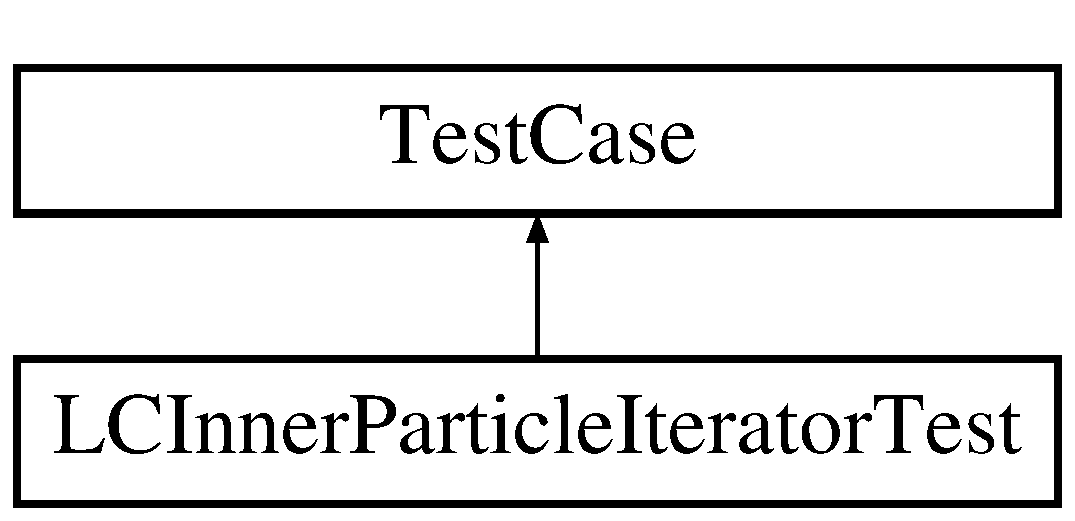
\includegraphics[height=2.000000cm]{classLCInnerParticleIteratorTest}
\end{center}
\end{figure}
\subsection*{Public Member Functions}
\begin{DoxyCompactItemize}
\item 
\hyperlink{classLCInnerParticleIteratorTest_ad3c783a3578588b75d6c973c428c84a3}{L\-C\-Inner\-Particle\-Iterator\-Test} ()
\item 
virtual \hyperlink{classLCInnerParticleIteratorTest_a4504aad35671ecb106c0987989dc8569}{$\sim$\-L\-C\-Inner\-Particle\-Iterator\-Test} ()
\item 
void \hyperlink{classLCInnerParticleIteratorTest_a1270bd9ac6d8d565b80576a21cb29787}{set\-Up} ()
\item 
void \hyperlink{classLCInnerParticleIteratorTest_a5e91e56ad97f4e9ff31a8c19192e88e0}{tear\-Down} ()
\item 
void \hyperlink{classLCInnerParticleIteratorTest_a691ec0fa8f46c909392b98bb90ded764}{test\-Particle\-Reference} ()
\item 
void \hyperlink{classLCInnerParticleIteratorTest_a36498adcccd66229a40b54acfa20ecca}{test\-Get\-Cell\-Number} ()
\item 
void \hyperlink{classLCInnerParticleIteratorTest_afd8b3239c190ef845b608d1d1ceb108c}{test\-Assignment} ()
\item 
void \hyperlink{classLCInnerParticleIteratorTest_af02554b593671d412559db8ff73ee19e}{test\-Inequality} ()
\item 
void \hyperlink{classLCInnerParticleIteratorTest_a6d1d41829ec37d5003b2cfcc48f475de}{test\-Iteration} ()
\item 
void \hyperlink{classLCInnerParticleIteratorTest_a201b0e7c640fdca8328f78ddc012abed}{test\-Check\-Left} ()
\item 
void \hyperlink{classLCInnerParticleIteratorTest_a25571212771d23d26a28028f5b643979}{test\-Check\-Right} ()
\item 
void \hyperlink{classLCInnerParticleIteratorTest_a8b2389225007973776f08a63b919653c}{test\-Check\-Bottom} ()
\item 
void \hyperlink{classLCInnerParticleIteratorTest_a23a5b0bd727f9056f764f9a548ca7916}{test\-Check\-Back} ()
\item 
void \hyperlink{classLCInnerParticleIteratorTest_ae0e5a407185c43795ca65f9f58e3a31d}{test\-Check\-Top} ()
\end{DoxyCompactItemize}
\subsection*{Static Public Member Functions}
\begin{DoxyCompactItemize}
\item 
static Test $\ast$ \hyperlink{classLCInnerParticleIteratorTest_a9426f3086943850f1b7c12d5f5276557}{suite} ()
\end{DoxyCompactItemize}
\subsection*{Private Attributes}
\begin{DoxyCompactItemize}
\item 
\hyperlink{classutils_1_1LCParticleContainer}{utils\-::\-L\-C\-Particle\-Container} \hyperlink{classLCInnerParticleIteratorTest_a8f9c568f79dbbe24bbd49a7cb5bea7f1}{container}
\item 
int \hyperlink{classLCInnerParticleIteratorTest_a05fd0158904ae918a9fa58d22fadfe98}{width}
\item 
int \hyperlink{classLCInnerParticleIteratorTest_a31a40948facb70846156b5c374e3465b}{height}
\item 
int \hyperlink{classLCInnerParticleIteratorTest_a154bfbcc8fbcaebb1a1e4a6139a0e822}{depth}
\item 
int \hyperlink{classLCInnerParticleIteratorTest_a0e1dbc80d10588e1089c689310dc6789}{num\-\_\-of\-\_\-cells}
\item 
double \hyperlink{classLCInnerParticleIteratorTest_a791b6f201aef3f978e65056980828704}{cutoff\-\_\-radius}
\item 
\hyperlink{classutils_1_1Vector}{utils\-::\-Vector}$<$ double, 3 $>$ \hyperlink{classLCInnerParticleIteratorTest_a9899df5843acade8a21c9f1b50a19fef}{domain\-\_\-size}
\item 
std\-::list$<$ \hyperlink{classParticle}{Particle} $>$ \hyperlink{classLCInnerParticleIteratorTest_a06041919ff77a8f00537ee269be27f25}{particles}
\end{DoxyCompactItemize}


\subsection{Constructor \& Destructor Documentation}
\hypertarget{classLCInnerParticleIteratorTest_ad3c783a3578588b75d6c973c428c84a3}{\index{L\-C\-Inner\-Particle\-Iterator\-Test@{L\-C\-Inner\-Particle\-Iterator\-Test}!L\-C\-Inner\-Particle\-Iterator\-Test@{L\-C\-Inner\-Particle\-Iterator\-Test}}
\index{L\-C\-Inner\-Particle\-Iterator\-Test@{L\-C\-Inner\-Particle\-Iterator\-Test}!LCInnerParticleIteratorTest@{L\-C\-Inner\-Particle\-Iterator\-Test}}
\subsubsection[{L\-C\-Inner\-Particle\-Iterator\-Test}]{\setlength{\rightskip}{0pt plus 5cm}L\-C\-Inner\-Particle\-Iterator\-Test\-::\-L\-C\-Inner\-Particle\-Iterator\-Test (
\begin{DoxyParamCaption}
{}
\end{DoxyParamCaption}
)}}\label{classLCInnerParticleIteratorTest_ad3c783a3578588b75d6c973c428c84a3}
\hypertarget{classLCInnerParticleIteratorTest_a4504aad35671ecb106c0987989dc8569}{\index{L\-C\-Inner\-Particle\-Iterator\-Test@{L\-C\-Inner\-Particle\-Iterator\-Test}!$\sim$\-L\-C\-Inner\-Particle\-Iterator\-Test@{$\sim$\-L\-C\-Inner\-Particle\-Iterator\-Test}}
\index{$\sim$\-L\-C\-Inner\-Particle\-Iterator\-Test@{$\sim$\-L\-C\-Inner\-Particle\-Iterator\-Test}!LCInnerParticleIteratorTest@{L\-C\-Inner\-Particle\-Iterator\-Test}}
\subsubsection[{$\sim$\-L\-C\-Inner\-Particle\-Iterator\-Test}]{\setlength{\rightskip}{0pt plus 5cm}L\-C\-Inner\-Particle\-Iterator\-Test\-::$\sim$\-L\-C\-Inner\-Particle\-Iterator\-Test (
\begin{DoxyParamCaption}
{}
\end{DoxyParamCaption}
)\hspace{0.3cm}{\ttfamily [virtual]}}}\label{classLCInnerParticleIteratorTest_a4504aad35671ecb106c0987989dc8569}


\subsection{Member Function Documentation}
\hypertarget{classLCInnerParticleIteratorTest_a1270bd9ac6d8d565b80576a21cb29787}{\index{L\-C\-Inner\-Particle\-Iterator\-Test@{L\-C\-Inner\-Particle\-Iterator\-Test}!set\-Up@{set\-Up}}
\index{set\-Up@{set\-Up}!LCInnerParticleIteratorTest@{L\-C\-Inner\-Particle\-Iterator\-Test}}
\subsubsection[{set\-Up}]{\setlength{\rightskip}{0pt plus 5cm}void L\-C\-Inner\-Particle\-Iterator\-Test\-::set\-Up (
\begin{DoxyParamCaption}
{}
\end{DoxyParamCaption}
)}}\label{classLCInnerParticleIteratorTest_a1270bd9ac6d8d565b80576a21cb29787}
process\-: Set up the test variables \hypertarget{classLCInnerParticleIteratorTest_a9426f3086943850f1b7c12d5f5276557}{\index{L\-C\-Inner\-Particle\-Iterator\-Test@{L\-C\-Inner\-Particle\-Iterator\-Test}!suite@{suite}}
\index{suite@{suite}!LCInnerParticleIteratorTest@{L\-C\-Inner\-Particle\-Iterator\-Test}}
\subsubsection[{suite}]{\setlength{\rightskip}{0pt plus 5cm}Cpp\-Unit\-::\-Test $\ast$ L\-C\-Inner\-Particle\-Iterator\-Test\-::suite (
\begin{DoxyParamCaption}
{}
\end{DoxyParamCaption}
)\hspace{0.3cm}{\ttfamily [static]}}}\label{classLCInnerParticleIteratorTest_a9426f3086943850f1b7c12d5f5276557}
\begin{DoxyReturn}{Returns}
the Test\-Suite for the tested methods of Particle\-Iterator 
\end{DoxyReturn}
\hypertarget{classLCInnerParticleIteratorTest_a5e91e56ad97f4e9ff31a8c19192e88e0}{\index{L\-C\-Inner\-Particle\-Iterator\-Test@{L\-C\-Inner\-Particle\-Iterator\-Test}!tear\-Down@{tear\-Down}}
\index{tear\-Down@{tear\-Down}!LCInnerParticleIteratorTest@{L\-C\-Inner\-Particle\-Iterator\-Test}}
\subsubsection[{tear\-Down}]{\setlength{\rightskip}{0pt plus 5cm}void L\-C\-Inner\-Particle\-Iterator\-Test\-::tear\-Down (
\begin{DoxyParamCaption}
{}
\end{DoxyParamCaption}
)}}\label{classLCInnerParticleIteratorTest_a5e91e56ad97f4e9ff31a8c19192e88e0}
Delete the variables \hypertarget{classLCInnerParticleIteratorTest_afd8b3239c190ef845b608d1d1ceb108c}{\index{L\-C\-Inner\-Particle\-Iterator\-Test@{L\-C\-Inner\-Particle\-Iterator\-Test}!test\-Assignment@{test\-Assignment}}
\index{test\-Assignment@{test\-Assignment}!LCInnerParticleIteratorTest@{L\-C\-Inner\-Particle\-Iterator\-Test}}
\subsubsection[{test\-Assignment}]{\setlength{\rightskip}{0pt plus 5cm}void L\-C\-Inner\-Particle\-Iterator\-Test\-::test\-Assignment (
\begin{DoxyParamCaption}
{}
\end{DoxyParamCaption}
)}}\label{classLCInnerParticleIteratorTest_afd8b3239c190ef845b608d1d1ceb108c}
\hypertarget{classLCInnerParticleIteratorTest_a23a5b0bd727f9056f764f9a548ca7916}{\index{L\-C\-Inner\-Particle\-Iterator\-Test@{L\-C\-Inner\-Particle\-Iterator\-Test}!test\-Check\-Back@{test\-Check\-Back}}
\index{test\-Check\-Back@{test\-Check\-Back}!LCInnerParticleIteratorTest@{L\-C\-Inner\-Particle\-Iterator\-Test}}
\subsubsection[{test\-Check\-Back}]{\setlength{\rightskip}{0pt plus 5cm}void L\-C\-Inner\-Particle\-Iterator\-Test\-::test\-Check\-Back (
\begin{DoxyParamCaption}
{}
\end{DoxyParamCaption}
)}}\label{classLCInnerParticleIteratorTest_a23a5b0bd727f9056f764f9a548ca7916}
\hypertarget{classLCInnerParticleIteratorTest_a8b2389225007973776f08a63b919653c}{\index{L\-C\-Inner\-Particle\-Iterator\-Test@{L\-C\-Inner\-Particle\-Iterator\-Test}!test\-Check\-Bottom@{test\-Check\-Bottom}}
\index{test\-Check\-Bottom@{test\-Check\-Bottom}!LCInnerParticleIteratorTest@{L\-C\-Inner\-Particle\-Iterator\-Test}}
\subsubsection[{test\-Check\-Bottom}]{\setlength{\rightskip}{0pt plus 5cm}void L\-C\-Inner\-Particle\-Iterator\-Test\-::test\-Check\-Bottom (
\begin{DoxyParamCaption}
{}
\end{DoxyParamCaption}
)}}\label{classLCInnerParticleIteratorTest_a8b2389225007973776f08a63b919653c}
\hypertarget{classLCInnerParticleIteratorTest_a201b0e7c640fdca8328f78ddc012abed}{\index{L\-C\-Inner\-Particle\-Iterator\-Test@{L\-C\-Inner\-Particle\-Iterator\-Test}!test\-Check\-Left@{test\-Check\-Left}}
\index{test\-Check\-Left@{test\-Check\-Left}!LCInnerParticleIteratorTest@{L\-C\-Inner\-Particle\-Iterator\-Test}}
\subsubsection[{test\-Check\-Left}]{\setlength{\rightskip}{0pt plus 5cm}void L\-C\-Inner\-Particle\-Iterator\-Test\-::test\-Check\-Left (
\begin{DoxyParamCaption}
{}
\end{DoxyParamCaption}
)}}\label{classLCInnerParticleIteratorTest_a201b0e7c640fdca8328f78ddc012abed}
\hypertarget{classLCInnerParticleIteratorTest_a25571212771d23d26a28028f5b643979}{\index{L\-C\-Inner\-Particle\-Iterator\-Test@{L\-C\-Inner\-Particle\-Iterator\-Test}!test\-Check\-Right@{test\-Check\-Right}}
\index{test\-Check\-Right@{test\-Check\-Right}!LCInnerParticleIteratorTest@{L\-C\-Inner\-Particle\-Iterator\-Test}}
\subsubsection[{test\-Check\-Right}]{\setlength{\rightskip}{0pt plus 5cm}void L\-C\-Inner\-Particle\-Iterator\-Test\-::test\-Check\-Right (
\begin{DoxyParamCaption}
{}
\end{DoxyParamCaption}
)}}\label{classLCInnerParticleIteratorTest_a25571212771d23d26a28028f5b643979}
\hypertarget{classLCInnerParticleIteratorTest_ae0e5a407185c43795ca65f9f58e3a31d}{\index{L\-C\-Inner\-Particle\-Iterator\-Test@{L\-C\-Inner\-Particle\-Iterator\-Test}!test\-Check\-Top@{test\-Check\-Top}}
\index{test\-Check\-Top@{test\-Check\-Top}!LCInnerParticleIteratorTest@{L\-C\-Inner\-Particle\-Iterator\-Test}}
\subsubsection[{test\-Check\-Top}]{\setlength{\rightskip}{0pt plus 5cm}void L\-C\-Inner\-Particle\-Iterator\-Test\-::test\-Check\-Top (
\begin{DoxyParamCaption}
{}
\end{DoxyParamCaption}
)}}\label{classLCInnerParticleIteratorTest_ae0e5a407185c43795ca65f9f58e3a31d}
\hypertarget{classLCInnerParticleIteratorTest_a36498adcccd66229a40b54acfa20ecca}{\index{L\-C\-Inner\-Particle\-Iterator\-Test@{L\-C\-Inner\-Particle\-Iterator\-Test}!test\-Get\-Cell\-Number@{test\-Get\-Cell\-Number}}
\index{test\-Get\-Cell\-Number@{test\-Get\-Cell\-Number}!LCInnerParticleIteratorTest@{L\-C\-Inner\-Particle\-Iterator\-Test}}
\subsubsection[{test\-Get\-Cell\-Number}]{\setlength{\rightskip}{0pt plus 5cm}void L\-C\-Inner\-Particle\-Iterator\-Test\-::test\-Get\-Cell\-Number (
\begin{DoxyParamCaption}
{}
\end{DoxyParamCaption}
)}}\label{classLCInnerParticleIteratorTest_a36498adcccd66229a40b54acfa20ecca}
\hypertarget{classLCInnerParticleIteratorTest_af02554b593671d412559db8ff73ee19e}{\index{L\-C\-Inner\-Particle\-Iterator\-Test@{L\-C\-Inner\-Particle\-Iterator\-Test}!test\-Inequality@{test\-Inequality}}
\index{test\-Inequality@{test\-Inequality}!LCInnerParticleIteratorTest@{L\-C\-Inner\-Particle\-Iterator\-Test}}
\subsubsection[{test\-Inequality}]{\setlength{\rightskip}{0pt plus 5cm}void L\-C\-Inner\-Particle\-Iterator\-Test\-::test\-Inequality (
\begin{DoxyParamCaption}
{}
\end{DoxyParamCaption}
)}}\label{classLCInnerParticleIteratorTest_af02554b593671d412559db8ff73ee19e}
Check the \char`\"{}!=\char`\"{} operator of the iterator \hypertarget{classLCInnerParticleIteratorTest_a6d1d41829ec37d5003b2cfcc48f475de}{\index{L\-C\-Inner\-Particle\-Iterator\-Test@{L\-C\-Inner\-Particle\-Iterator\-Test}!test\-Iteration@{test\-Iteration}}
\index{test\-Iteration@{test\-Iteration}!LCInnerParticleIteratorTest@{L\-C\-Inner\-Particle\-Iterator\-Test}}
\subsubsection[{test\-Iteration}]{\setlength{\rightskip}{0pt plus 5cm}void L\-C\-Inner\-Particle\-Iterator\-Test\-::test\-Iteration (
\begin{DoxyParamCaption}
{}
\end{DoxyParamCaption}
)}}\label{classLCInnerParticleIteratorTest_a6d1d41829ec37d5003b2cfcc48f475de}
Check the \char`\"{}++\char`\"{} operator of the iterator \hypertarget{classLCInnerParticleIteratorTest_a691ec0fa8f46c909392b98bb90ded764}{\index{L\-C\-Inner\-Particle\-Iterator\-Test@{L\-C\-Inner\-Particle\-Iterator\-Test}!test\-Particle\-Reference@{test\-Particle\-Reference}}
\index{test\-Particle\-Reference@{test\-Particle\-Reference}!LCInnerParticleIteratorTest@{L\-C\-Inner\-Particle\-Iterator\-Test}}
\subsubsection[{test\-Particle\-Reference}]{\setlength{\rightskip}{0pt plus 5cm}void L\-C\-Inner\-Particle\-Iterator\-Test\-::test\-Particle\-Reference (
\begin{DoxyParamCaption}
{}
\end{DoxyParamCaption}
)}}\label{classLCInnerParticleIteratorTest_a691ec0fa8f46c909392b98bb90ded764}
Check the \char`\"{}$\ast$\char`\"{} operator of the iterator 

\subsection{Member Data Documentation}
\hypertarget{classLCInnerParticleIteratorTest_a8f9c568f79dbbe24bbd49a7cb5bea7f1}{\index{L\-C\-Inner\-Particle\-Iterator\-Test@{L\-C\-Inner\-Particle\-Iterator\-Test}!container@{container}}
\index{container@{container}!LCInnerParticleIteratorTest@{L\-C\-Inner\-Particle\-Iterator\-Test}}
\subsubsection[{container}]{\setlength{\rightskip}{0pt plus 5cm}{\bf utils\-::\-L\-C\-Particle\-Container} L\-C\-Inner\-Particle\-Iterator\-Test\-::container\hspace{0.3cm}{\ttfamily [private]}}}\label{classLCInnerParticleIteratorTest_a8f9c568f79dbbe24bbd49a7cb5bea7f1}
The particle container to check the Iterator \hypertarget{classLCInnerParticleIteratorTest_a791b6f201aef3f978e65056980828704}{\index{L\-C\-Inner\-Particle\-Iterator\-Test@{L\-C\-Inner\-Particle\-Iterator\-Test}!cutoff\-\_\-radius@{cutoff\-\_\-radius}}
\index{cutoff\-\_\-radius@{cutoff\-\_\-radius}!LCInnerParticleIteratorTest@{L\-C\-Inner\-Particle\-Iterator\-Test}}
\subsubsection[{cutoff\-\_\-radius}]{\setlength{\rightskip}{0pt plus 5cm}double L\-C\-Inner\-Particle\-Iterator\-Test\-::cutoff\-\_\-radius\hspace{0.3cm}{\ttfamily [private]}}}\label{classLCInnerParticleIteratorTest_a791b6f201aef3f978e65056980828704}
\hypertarget{classLCInnerParticleIteratorTest_a154bfbcc8fbcaebb1a1e4a6139a0e822}{\index{L\-C\-Inner\-Particle\-Iterator\-Test@{L\-C\-Inner\-Particle\-Iterator\-Test}!depth@{depth}}
\index{depth@{depth}!LCInnerParticleIteratorTest@{L\-C\-Inner\-Particle\-Iterator\-Test}}
\subsubsection[{depth}]{\setlength{\rightskip}{0pt plus 5cm}int L\-C\-Inner\-Particle\-Iterator\-Test\-::depth\hspace{0.3cm}{\ttfamily [private]}}}\label{classLCInnerParticleIteratorTest_a154bfbcc8fbcaebb1a1e4a6139a0e822}
\hypertarget{classLCInnerParticleIteratorTest_a9899df5843acade8a21c9f1b50a19fef}{\index{L\-C\-Inner\-Particle\-Iterator\-Test@{L\-C\-Inner\-Particle\-Iterator\-Test}!domain\-\_\-size@{domain\-\_\-size}}
\index{domain\-\_\-size@{domain\-\_\-size}!LCInnerParticleIteratorTest@{L\-C\-Inner\-Particle\-Iterator\-Test}}
\subsubsection[{domain\-\_\-size}]{\setlength{\rightskip}{0pt plus 5cm}{\bf utils\-::\-Vector}$<$double, 3$>$ L\-C\-Inner\-Particle\-Iterator\-Test\-::domain\-\_\-size\hspace{0.3cm}{\ttfamily [private]}}}\label{classLCInnerParticleIteratorTest_a9899df5843acade8a21c9f1b50a19fef}
\hypertarget{classLCInnerParticleIteratorTest_a31a40948facb70846156b5c374e3465b}{\index{L\-C\-Inner\-Particle\-Iterator\-Test@{L\-C\-Inner\-Particle\-Iterator\-Test}!height@{height}}
\index{height@{height}!LCInnerParticleIteratorTest@{L\-C\-Inner\-Particle\-Iterator\-Test}}
\subsubsection[{height}]{\setlength{\rightskip}{0pt plus 5cm}int L\-C\-Inner\-Particle\-Iterator\-Test\-::height\hspace{0.3cm}{\ttfamily [private]}}}\label{classLCInnerParticleIteratorTest_a31a40948facb70846156b5c374e3465b}
\hypertarget{classLCInnerParticleIteratorTest_a0e1dbc80d10588e1089c689310dc6789}{\index{L\-C\-Inner\-Particle\-Iterator\-Test@{L\-C\-Inner\-Particle\-Iterator\-Test}!num\-\_\-of\-\_\-cells@{num\-\_\-of\-\_\-cells}}
\index{num\-\_\-of\-\_\-cells@{num\-\_\-of\-\_\-cells}!LCInnerParticleIteratorTest@{L\-C\-Inner\-Particle\-Iterator\-Test}}
\subsubsection[{num\-\_\-of\-\_\-cells}]{\setlength{\rightskip}{0pt plus 5cm}int L\-C\-Inner\-Particle\-Iterator\-Test\-::num\-\_\-of\-\_\-cells\hspace{0.3cm}{\ttfamily [private]}}}\label{classLCInnerParticleIteratorTest_a0e1dbc80d10588e1089c689310dc6789}
\hypertarget{classLCInnerParticleIteratorTest_a06041919ff77a8f00537ee269be27f25}{\index{L\-C\-Inner\-Particle\-Iterator\-Test@{L\-C\-Inner\-Particle\-Iterator\-Test}!particles@{particles}}
\index{particles@{particles}!LCInnerParticleIteratorTest@{L\-C\-Inner\-Particle\-Iterator\-Test}}
\subsubsection[{particles}]{\setlength{\rightskip}{0pt plus 5cm}std\-::list$<${\bf Particle}$>$ L\-C\-Inner\-Particle\-Iterator\-Test\-::particles\hspace{0.3cm}{\ttfamily [private]}}}\label{classLCInnerParticleIteratorTest_a06041919ff77a8f00537ee269be27f25}
The particle list, which will be used to compare to the container \hypertarget{classLCInnerParticleIteratorTest_a05fd0158904ae918a9fa58d22fadfe98}{\index{L\-C\-Inner\-Particle\-Iterator\-Test@{L\-C\-Inner\-Particle\-Iterator\-Test}!width@{width}}
\index{width@{width}!LCInnerParticleIteratorTest@{L\-C\-Inner\-Particle\-Iterator\-Test}}
\subsubsection[{width}]{\setlength{\rightskip}{0pt plus 5cm}int L\-C\-Inner\-Particle\-Iterator\-Test\-::width\hspace{0.3cm}{\ttfamily [private]}}}\label{classLCInnerParticleIteratorTest_a05fd0158904ae918a9fa58d22fadfe98}


The documentation for this class was generated from the following files\-:\begin{DoxyCompactItemize}
\item 
src/tests/\hyperlink{LCInnerParticleIteratorTest_8h}{L\-C\-Inner\-Particle\-Iterator\-Test.\-h}\item 
src/tests/\hyperlink{LCInnerParticleIteratorTest_8cpp}{L\-C\-Inner\-Particle\-Iterator\-Test.\-cpp}\end{DoxyCompactItemize}

\hypertarget{classutils_1_1LCOuterParticleIterator}{\section{utils\-:\-:L\-C\-Outer\-Particle\-Iterator Class Reference}
\label{classutils_1_1LCOuterParticleIterator}\index{utils\-::\-L\-C\-Outer\-Particle\-Iterator@{utils\-::\-L\-C\-Outer\-Particle\-Iterator}}
}


{\ttfamily \#include $<$L\-C\-Outer\-Particle\-Iterator.\-h$>$}

\subsection*{Public Member Functions}
\begin{DoxyCompactItemize}
\item 
\hyperlink{classutils_1_1LCOuterParticleIterator_a9ac0d0f665d39b1cd9ffd3e9f07e5155}{L\-C\-Outer\-Particle\-Iterator} ()
\item 
\hyperlink{classutils_1_1LCOuterParticleIterator_ab399d6d6b97cb09e53217d9654ae9a64}{L\-C\-Outer\-Particle\-Iterator} (int cell\-\_\-size\-\_\-arg, std\-::vector$<$ std\-::list$<$ \hyperlink{classParticle}{Particle} $\ast$ $>$ $\ast$ $>$ $\ast$cells\-\_\-arg, std\-::list$<$ \hyperlink{classParticle}{Particle} $\ast$ $>$\-::\hyperlink{classutils_1_1LCOuterParticleIterator_ab01cb9c518e6f5e97b4b99b8a1af88e5}{iterator} iterator\-\_\-arg, int index\-\_\-arg)
\item 
virtual \hyperlink{classutils_1_1LCOuterParticleIterator_a3a66099197abb8723e1bd546cdbdafb5}{$\sim$\-L\-C\-Outer\-Particle\-Iterator} ()
\item 
\hyperlink{classParticle}{Particle} \& \hyperlink{classutils_1_1LCOuterParticleIterator_acaf99d121ac0d78370bbc479a7c6448d}{operator$\ast$} () const 
\item 
void \hyperlink{classutils_1_1LCOuterParticleIterator_a8257913f53e484b3e544882a53571d05}{operator++} ()
\item 
int \hyperlink{classutils_1_1LCOuterParticleIterator_a31776769fce3238c1d76a442000f2b23}{get\-Cell\-Number} ()
\item 
std\-::list$<$ \hyperlink{classParticle}{Particle} $\ast$ $>$\-::\hyperlink{classutils_1_1LCOuterParticleIterator_ab01cb9c518e6f5e97b4b99b8a1af88e5}{iterator} \hyperlink{classutils_1_1LCOuterParticleIterator_add4758ecb5c0da6b60d0105b7b497b80}{get\-Iterator} ()
\item 
bool \hyperlink{classutils_1_1LCOuterParticleIterator_a8ca9661e34d7a0750544b6bc211c87be}{operator!=} (const \hyperlink{classutils_1_1LCOuterParticleIterator}{L\-C\-Outer\-Particle\-Iterator} b)
\item 
\hyperlink{classutils_1_1LCOuterParticleIterator}{L\-C\-Outer\-Particle\-Iterator} \& \hyperlink{classutils_1_1LCOuterParticleIterator_afcaf7fb20f9711329a011af367bec64c}{operator=} (const \hyperlink{classutils_1_1LCOuterParticleIterator}{L\-C\-Outer\-Particle\-Iterator} \&cpy)
\end{DoxyCompactItemize}
\subsection*{Private Attributes}
\begin{DoxyCompactItemize}
\item 
std\-::vector$<$ std\-::list\\*
$<$ \hyperlink{classParticle}{Particle} $\ast$ $>$ $\ast$ $>$ $\ast$ \hyperlink{classutils_1_1LCOuterParticleIterator_a2a9cde56a9eab6ba0dad00cfad74ff01}{cells}
\item 
int \hyperlink{classutils_1_1LCOuterParticleIterator_aa4df9b61c19d57586aa8a24433df3bb9}{cell\-\_\-size}
\item 
int \hyperlink{classutils_1_1LCOuterParticleIterator_a54059f42735afc424f37d05cb5a40a98}{index}
\item 
std\-::list$<$ \hyperlink{classParticle}{Particle} $\ast$ $>$\-::iterator \hyperlink{classutils_1_1LCOuterParticleIterator_ab01cb9c518e6f5e97b4b99b8a1af88e5}{iterator}
\end{DoxyCompactItemize}


\subsection{Constructor \& Destructor Documentation}
\hypertarget{classutils_1_1LCOuterParticleIterator_a9ac0d0f665d39b1cd9ffd3e9f07e5155}{\index{utils\-::\-L\-C\-Outer\-Particle\-Iterator@{utils\-::\-L\-C\-Outer\-Particle\-Iterator}!L\-C\-Outer\-Particle\-Iterator@{L\-C\-Outer\-Particle\-Iterator}}
\index{L\-C\-Outer\-Particle\-Iterator@{L\-C\-Outer\-Particle\-Iterator}!utils::LCOuterParticleIterator@{utils\-::\-L\-C\-Outer\-Particle\-Iterator}}
\subsubsection[{L\-C\-Outer\-Particle\-Iterator}]{\setlength{\rightskip}{0pt plus 5cm}utils\-::\-L\-C\-Outer\-Particle\-Iterator\-::\-L\-C\-Outer\-Particle\-Iterator (
\begin{DoxyParamCaption}
{}
\end{DoxyParamCaption}
)}}\label{classutils_1_1LCOuterParticleIterator_a9ac0d0f665d39b1cd9ffd3e9f07e5155}
\hypertarget{classutils_1_1LCOuterParticleIterator_ab399d6d6b97cb09e53217d9654ae9a64}{\index{utils\-::\-L\-C\-Outer\-Particle\-Iterator@{utils\-::\-L\-C\-Outer\-Particle\-Iterator}!L\-C\-Outer\-Particle\-Iterator@{L\-C\-Outer\-Particle\-Iterator}}
\index{L\-C\-Outer\-Particle\-Iterator@{L\-C\-Outer\-Particle\-Iterator}!utils::LCOuterParticleIterator@{utils\-::\-L\-C\-Outer\-Particle\-Iterator}}
\subsubsection[{L\-C\-Outer\-Particle\-Iterator}]{\setlength{\rightskip}{0pt plus 5cm}utils\-::\-L\-C\-Outer\-Particle\-Iterator\-::\-L\-C\-Outer\-Particle\-Iterator (
\begin{DoxyParamCaption}
\item[{int}]{cell\-\_\-size\-\_\-arg, }
\item[{std\-::vector$<$ std\-::list$<$ {\bf Particle} $\ast$ $>$ $\ast$ $>$ $\ast$}]{cells\-\_\-arg, }
\item[{std\-::list$<$ {\bf Particle} $\ast$ $>$\-::{\bf iterator}}]{iterator\-\_\-arg, }
\item[{int}]{index\-\_\-arg}
\end{DoxyParamCaption}
)}}\label{classutils_1_1LCOuterParticleIterator_ab399d6d6b97cb09e53217d9654ae9a64}
\hypertarget{classutils_1_1LCOuterParticleIterator_a3a66099197abb8723e1bd546cdbdafb5}{\index{utils\-::\-L\-C\-Outer\-Particle\-Iterator@{utils\-::\-L\-C\-Outer\-Particle\-Iterator}!$\sim$\-L\-C\-Outer\-Particle\-Iterator@{$\sim$\-L\-C\-Outer\-Particle\-Iterator}}
\index{$\sim$\-L\-C\-Outer\-Particle\-Iterator@{$\sim$\-L\-C\-Outer\-Particle\-Iterator}!utils::LCOuterParticleIterator@{utils\-::\-L\-C\-Outer\-Particle\-Iterator}}
\subsubsection[{$\sim$\-L\-C\-Outer\-Particle\-Iterator}]{\setlength{\rightskip}{0pt plus 5cm}utils\-::\-L\-C\-Outer\-Particle\-Iterator\-::$\sim$\-L\-C\-Outer\-Particle\-Iterator (
\begin{DoxyParamCaption}
{}
\end{DoxyParamCaption}
)\hspace{0.3cm}{\ttfamily [virtual]}}}\label{classutils_1_1LCOuterParticleIterator_a3a66099197abb8723e1bd546cdbdafb5}


\subsection{Member Function Documentation}
\hypertarget{classutils_1_1LCOuterParticleIterator_a31776769fce3238c1d76a442000f2b23}{\index{utils\-::\-L\-C\-Outer\-Particle\-Iterator@{utils\-::\-L\-C\-Outer\-Particle\-Iterator}!get\-Cell\-Number@{get\-Cell\-Number}}
\index{get\-Cell\-Number@{get\-Cell\-Number}!utils::LCOuterParticleIterator@{utils\-::\-L\-C\-Outer\-Particle\-Iterator}}
\subsubsection[{get\-Cell\-Number}]{\setlength{\rightskip}{0pt plus 5cm}int utils\-::\-L\-C\-Outer\-Particle\-Iterator\-::get\-Cell\-Number (
\begin{DoxyParamCaption}
{}
\end{DoxyParamCaption}
)}}\label{classutils_1_1LCOuterParticleIterator_a31776769fce3238c1d76a442000f2b23}
\begin{DoxyReturn}{Returns}
the cell number of the outer iterator 
\end{DoxyReturn}
\hypertarget{classutils_1_1LCOuterParticleIterator_add4758ecb5c0da6b60d0105b7b497b80}{\index{utils\-::\-L\-C\-Outer\-Particle\-Iterator@{utils\-::\-L\-C\-Outer\-Particle\-Iterator}!get\-Iterator@{get\-Iterator}}
\index{get\-Iterator@{get\-Iterator}!utils::LCOuterParticleIterator@{utils\-::\-L\-C\-Outer\-Particle\-Iterator}}
\subsubsection[{get\-Iterator}]{\setlength{\rightskip}{0pt plus 5cm}std\-::list$<$ {\bf Particle} $\ast$ $>$\-::{\bf iterator} utils\-::\-L\-C\-Outer\-Particle\-Iterator\-::get\-Iterator (
\begin{DoxyParamCaption}
{}
\end{DoxyParamCaption}
)}}\label{classutils_1_1LCOuterParticleIterator_add4758ecb5c0da6b60d0105b7b497b80}
\begin{DoxyReturn}{Returns}
the iterator 
\end{DoxyReturn}
\hypertarget{classutils_1_1LCOuterParticleIterator_a8ca9661e34d7a0750544b6bc211c87be}{\index{utils\-::\-L\-C\-Outer\-Particle\-Iterator@{utils\-::\-L\-C\-Outer\-Particle\-Iterator}!operator!=@{operator!=}}
\index{operator!=@{operator!=}!utils::LCOuterParticleIterator@{utils\-::\-L\-C\-Outer\-Particle\-Iterator}}
\subsubsection[{operator!=}]{\setlength{\rightskip}{0pt plus 5cm}bool utils\-::\-L\-C\-Outer\-Particle\-Iterator\-::operator!= (
\begin{DoxyParamCaption}
\item[{const {\bf L\-C\-Outer\-Particle\-Iterator}}]{b}
\end{DoxyParamCaption}
)}}\label{classutils_1_1LCOuterParticleIterator_a8ca9661e34d7a0750544b6bc211c87be}
checks on inequality 
\begin{DoxyParams}{Parameters}
{\em b} & the Iterator to compare with \\
\hline
\end{DoxyParams}
\begin{DoxyReturn}{Returns}
returns true, if the two iterators don't match 
\end{DoxyReturn}
\hypertarget{classutils_1_1LCOuterParticleIterator_acaf99d121ac0d78370bbc479a7c6448d}{\index{utils\-::\-L\-C\-Outer\-Particle\-Iterator@{utils\-::\-L\-C\-Outer\-Particle\-Iterator}!operator$\ast$@{operator$\ast$}}
\index{operator$\ast$@{operator$\ast$}!utils::LCOuterParticleIterator@{utils\-::\-L\-C\-Outer\-Particle\-Iterator}}
\subsubsection[{operator$\ast$}]{\setlength{\rightskip}{0pt plus 5cm}{\bf Particle} \& utils\-::\-L\-C\-Outer\-Particle\-Iterator\-::operator$\ast$ (
\begin{DoxyParamCaption}
{}
\end{DoxyParamCaption}
) const}}\label{classutils_1_1LCOuterParticleIterator_acaf99d121ac0d78370bbc479a7c6448d}
\begin{DoxyReturn}{Returns}
returns the reference to the momentary particle 
\end{DoxyReturn}
\hypertarget{classutils_1_1LCOuterParticleIterator_a8257913f53e484b3e544882a53571d05}{\index{utils\-::\-L\-C\-Outer\-Particle\-Iterator@{utils\-::\-L\-C\-Outer\-Particle\-Iterator}!operator++@{operator++}}
\index{operator++@{operator++}!utils::LCOuterParticleIterator@{utils\-::\-L\-C\-Outer\-Particle\-Iterator}}
\subsubsection[{operator++}]{\setlength{\rightskip}{0pt plus 5cm}void utils\-::\-L\-C\-Outer\-Particle\-Iterator\-::operator++ (
\begin{DoxyParamCaption}
{}
\end{DoxyParamCaption}
)}}\label{classutils_1_1LCOuterParticleIterator_a8257913f53e484b3e544882a53571d05}
iterates to the next element \hypertarget{classutils_1_1LCOuterParticleIterator_afcaf7fb20f9711329a011af367bec64c}{\index{utils\-::\-L\-C\-Outer\-Particle\-Iterator@{utils\-::\-L\-C\-Outer\-Particle\-Iterator}!operator=@{operator=}}
\index{operator=@{operator=}!utils::LCOuterParticleIterator@{utils\-::\-L\-C\-Outer\-Particle\-Iterator}}
\subsubsection[{operator=}]{\setlength{\rightskip}{0pt plus 5cm}{\bf L\-C\-Outer\-Particle\-Iterator} \& utils\-::\-L\-C\-Outer\-Particle\-Iterator\-::operator= (
\begin{DoxyParamCaption}
\item[{const {\bf L\-C\-Outer\-Particle\-Iterator} \&}]{cpy}
\end{DoxyParamCaption}
)}}\label{classutils_1_1LCOuterParticleIterator_afcaf7fb20f9711329a011af367bec64c}
\begin{DoxyReturn}{Returns}
assigns an outer iterator with the attributes of cpy 
\end{DoxyReturn}


\subsection{Member Data Documentation}
\hypertarget{classutils_1_1LCOuterParticleIterator_aa4df9b61c19d57586aa8a24433df3bb9}{\index{utils\-::\-L\-C\-Outer\-Particle\-Iterator@{utils\-::\-L\-C\-Outer\-Particle\-Iterator}!cell\-\_\-size@{cell\-\_\-size}}
\index{cell\-\_\-size@{cell\-\_\-size}!utils::LCOuterParticleIterator@{utils\-::\-L\-C\-Outer\-Particle\-Iterator}}
\subsubsection[{cell\-\_\-size}]{\setlength{\rightskip}{0pt plus 5cm}int utils\-::\-L\-C\-Outer\-Particle\-Iterator\-::cell\-\_\-size\hspace{0.3cm}{\ttfamily [private]}}}\label{classutils_1_1LCOuterParticleIterator_aa4df9b61c19d57586aa8a24433df3bb9}
the total number of cells \hypertarget{classutils_1_1LCOuterParticleIterator_a2a9cde56a9eab6ba0dad00cfad74ff01}{\index{utils\-::\-L\-C\-Outer\-Particle\-Iterator@{utils\-::\-L\-C\-Outer\-Particle\-Iterator}!cells@{cells}}
\index{cells@{cells}!utils::LCOuterParticleIterator@{utils\-::\-L\-C\-Outer\-Particle\-Iterator}}
\subsubsection[{cells}]{\setlength{\rightskip}{0pt plus 5cm}std\-::vector$<$std\-::list$<${\bf Particle} $\ast$$>$ $\ast$$>$$\ast$ utils\-::\-L\-C\-Outer\-Particle\-Iterator\-::cells\hspace{0.3cm}{\ttfamily [private]}}}\label{classutils_1_1LCOuterParticleIterator_a2a9cde56a9eab6ba0dad00cfad74ff01}
the cells of the domain \hypertarget{classutils_1_1LCOuterParticleIterator_a54059f42735afc424f37d05cb5a40a98}{\index{utils\-::\-L\-C\-Outer\-Particle\-Iterator@{utils\-::\-L\-C\-Outer\-Particle\-Iterator}!index@{index}}
\index{index@{index}!utils::LCOuterParticleIterator@{utils\-::\-L\-C\-Outer\-Particle\-Iterator}}
\subsubsection[{index}]{\setlength{\rightskip}{0pt plus 5cm}int utils\-::\-L\-C\-Outer\-Particle\-Iterator\-::index\hspace{0.3cm}{\ttfamily [private]}}}\label{classutils_1_1LCOuterParticleIterator_a54059f42735afc424f37d05cb5a40a98}
the cell number of the outer iterator \hypertarget{classutils_1_1LCOuterParticleIterator_ab01cb9c518e6f5e97b4b99b8a1af88e5}{\index{utils\-::\-L\-C\-Outer\-Particle\-Iterator@{utils\-::\-L\-C\-Outer\-Particle\-Iterator}!iterator@{iterator}}
\index{iterator@{iterator}!utils::LCOuterParticleIterator@{utils\-::\-L\-C\-Outer\-Particle\-Iterator}}
\subsubsection[{iterator}]{\setlength{\rightskip}{0pt plus 5cm}std\-::list$<${\bf Particle} $\ast$$>$\-::iterator utils\-::\-L\-C\-Outer\-Particle\-Iterator\-::iterator\hspace{0.3cm}{\ttfamily [private]}}}\label{classutils_1_1LCOuterParticleIterator_ab01cb9c518e6f5e97b4b99b8a1af88e5}
the iterator 

The documentation for this class was generated from the following files\-:\begin{DoxyCompactItemize}
\item 
src/utils/\hyperlink{LCOuterParticleIterator_8h}{L\-C\-Outer\-Particle\-Iterator.\-h}\item 
src/utils/\hyperlink{LCOuterParticleIterator_8cpp}{L\-C\-Outer\-Particle\-Iterator.\-cpp}\end{DoxyCompactItemize}

\hypertarget{classLCOuterParticleIteratorTest}{\section{L\-C\-Outer\-Particle\-Iterator\-Test Class Reference}
\label{classLCOuterParticleIteratorTest}\index{L\-C\-Outer\-Particle\-Iterator\-Test@{L\-C\-Outer\-Particle\-Iterator\-Test}}
}


{\ttfamily \#include $<$L\-C\-Outer\-Particle\-Iterator\-Test.\-h$>$}

Inheritance diagram for L\-C\-Outer\-Particle\-Iterator\-Test\-:\begin{figure}[H]
\begin{center}
\leavevmode
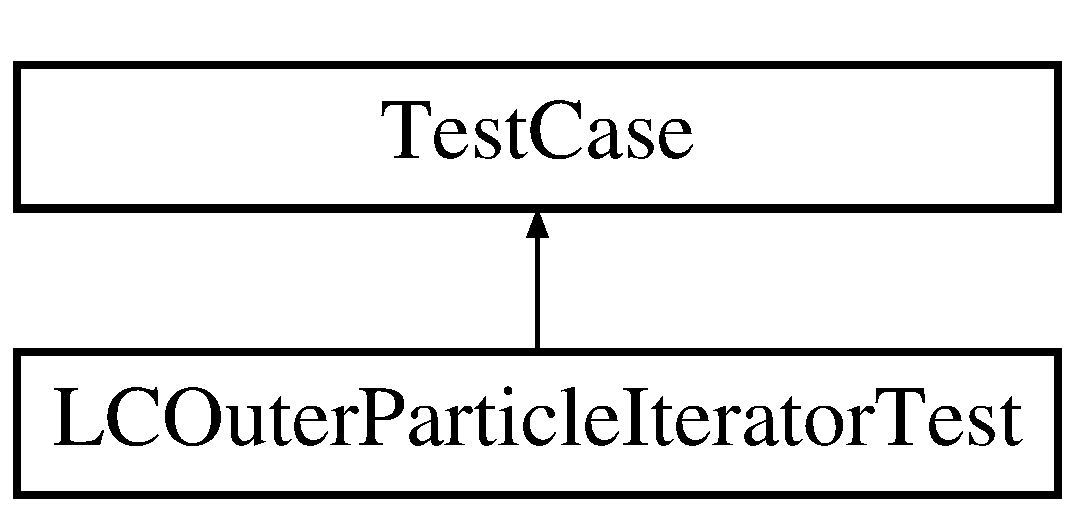
\includegraphics[height=2.000000cm]{classLCOuterParticleIteratorTest}
\end{center}
\end{figure}
\subsection*{Public Member Functions}
\begin{DoxyCompactItemize}
\item 
\hyperlink{classLCOuterParticleIteratorTest_aab7e474bcfba162d4d460d4b2018282c}{L\-C\-Outer\-Particle\-Iterator\-Test} ()
\item 
virtual \hyperlink{classLCOuterParticleIteratorTest_ad1ee78ab877c44be37b356f5c5b97854}{$\sim$\-L\-C\-Outer\-Particle\-Iterator\-Test} ()
\item 
void \hyperlink{classLCOuterParticleIteratorTest_a5a6f1dae02d5a9cab63956c4742f8831}{set\-Up} ()
\item 
void \hyperlink{classLCOuterParticleIteratorTest_a519ccd258d5d5ff815eb625865b436a0}{tear\-Down} ()
\item 
void \hyperlink{classLCOuterParticleIteratorTest_ad808d188130e9d259d18beb4cc879403}{test\-Inequality} ()
\item 
void \hyperlink{classLCOuterParticleIteratorTest_a671c0ec78e4b05aa68d4ddfa3702e72a}{test\-Assignment} ()
\item 
void \hyperlink{classLCOuterParticleIteratorTest_a9a239206cec7ee893db0ea0b084f8f4c}{test\-Particle\-Reference} ()
\item 
void \hyperlink{classLCOuterParticleIteratorTest_a6d3b51b7c2ffc2db75bdcd1fa896590f}{test\-Iteration} ()
\item 
void \hyperlink{classLCOuterParticleIteratorTest_a43cedd5dea09cb497bc214e6ebc7cf0f}{test\-Get\-Iterator} ()
\item 
void \hyperlink{classLCOuterParticleIteratorTest_a6fab4347a3aaa0d0c876055d6577332f}{test\-Get\-Cell\-Number} ()
\end{DoxyCompactItemize}
\subsection*{Static Public Member Functions}
\begin{DoxyCompactItemize}
\item 
static Test $\ast$ \hyperlink{classLCOuterParticleIteratorTest_a605097ed032fa017ae7a00025ef3c5ea}{suite} ()
\end{DoxyCompactItemize}
\subsection*{Private Attributes}
\begin{DoxyCompactItemize}
\item 
\hyperlink{classutils_1_1LCParticleContainer}{utils\-::\-L\-C\-Particle\-Container} \hyperlink{classLCOuterParticleIteratorTest_a70319a9d4b610f52fdcde19837acf4c0}{container}
\item 
int \hyperlink{classLCOuterParticleIteratorTest_a96d9f30988e98be898040163df3cad44}{width}
\item 
int \hyperlink{classLCOuterParticleIteratorTest_a35de94b14ffb7f81395cfba9fa9971f6}{height}
\item 
int \hyperlink{classLCOuterParticleIteratorTest_a5f7049990f80550d96e97ecea2da7b9f}{depth}
\item 
int \hyperlink{classLCOuterParticleIteratorTest_ac43a83d9555b5dd0c96274fa81aeb4e5}{cutoff\-\_\-radius}
\item 
int \hyperlink{classLCOuterParticleIteratorTest_aea461d3938bd39de26d5895a6cc1d133}{num\-\_\-of\-\_\-cells}
\item 
\hyperlink{classutils_1_1Vector}{utils\-::\-Vector}$<$ double, 3 $>$ \hyperlink{classLCOuterParticleIteratorTest_a74f89f909e41cd78b3d1ed13e7a71d59}{domain\-\_\-size}
\item 
std\-::list$<$ \hyperlink{classParticle}{Particle} $>$ \hyperlink{classLCOuterParticleIteratorTest_a77f1f60f85cf5d0350c8949918659b32}{particles}
\end{DoxyCompactItemize}


\subsection{Constructor \& Destructor Documentation}
\hypertarget{classLCOuterParticleIteratorTest_aab7e474bcfba162d4d460d4b2018282c}{\index{L\-C\-Outer\-Particle\-Iterator\-Test@{L\-C\-Outer\-Particle\-Iterator\-Test}!L\-C\-Outer\-Particle\-Iterator\-Test@{L\-C\-Outer\-Particle\-Iterator\-Test}}
\index{L\-C\-Outer\-Particle\-Iterator\-Test@{L\-C\-Outer\-Particle\-Iterator\-Test}!LCOuterParticleIteratorTest@{L\-C\-Outer\-Particle\-Iterator\-Test}}
\subsubsection[{L\-C\-Outer\-Particle\-Iterator\-Test}]{\setlength{\rightskip}{0pt plus 5cm}L\-C\-Outer\-Particle\-Iterator\-Test\-::\-L\-C\-Outer\-Particle\-Iterator\-Test (
\begin{DoxyParamCaption}
{}
\end{DoxyParamCaption}
)}}\label{classLCOuterParticleIteratorTest_aab7e474bcfba162d4d460d4b2018282c}
\hypertarget{classLCOuterParticleIteratorTest_ad1ee78ab877c44be37b356f5c5b97854}{\index{L\-C\-Outer\-Particle\-Iterator\-Test@{L\-C\-Outer\-Particle\-Iterator\-Test}!$\sim$\-L\-C\-Outer\-Particle\-Iterator\-Test@{$\sim$\-L\-C\-Outer\-Particle\-Iterator\-Test}}
\index{$\sim$\-L\-C\-Outer\-Particle\-Iterator\-Test@{$\sim$\-L\-C\-Outer\-Particle\-Iterator\-Test}!LCOuterParticleIteratorTest@{L\-C\-Outer\-Particle\-Iterator\-Test}}
\subsubsection[{$\sim$\-L\-C\-Outer\-Particle\-Iterator\-Test}]{\setlength{\rightskip}{0pt plus 5cm}L\-C\-Outer\-Particle\-Iterator\-Test\-::$\sim$\-L\-C\-Outer\-Particle\-Iterator\-Test (
\begin{DoxyParamCaption}
{}
\end{DoxyParamCaption}
)\hspace{0.3cm}{\ttfamily [virtual]}}}\label{classLCOuterParticleIteratorTest_ad1ee78ab877c44be37b356f5c5b97854}


\subsection{Member Function Documentation}
\hypertarget{classLCOuterParticleIteratorTest_a5a6f1dae02d5a9cab63956c4742f8831}{\index{L\-C\-Outer\-Particle\-Iterator\-Test@{L\-C\-Outer\-Particle\-Iterator\-Test}!set\-Up@{set\-Up}}
\index{set\-Up@{set\-Up}!LCOuterParticleIteratorTest@{L\-C\-Outer\-Particle\-Iterator\-Test}}
\subsubsection[{set\-Up}]{\setlength{\rightskip}{0pt plus 5cm}void L\-C\-Outer\-Particle\-Iterator\-Test\-::set\-Up (
\begin{DoxyParamCaption}
{}
\end{DoxyParamCaption}
)}}\label{classLCOuterParticleIteratorTest_a5a6f1dae02d5a9cab63956c4742f8831}
process\-: Set up the test variables \hypertarget{classLCOuterParticleIteratorTest_a605097ed032fa017ae7a00025ef3c5ea}{\index{L\-C\-Outer\-Particle\-Iterator\-Test@{L\-C\-Outer\-Particle\-Iterator\-Test}!suite@{suite}}
\index{suite@{suite}!LCOuterParticleIteratorTest@{L\-C\-Outer\-Particle\-Iterator\-Test}}
\subsubsection[{suite}]{\setlength{\rightskip}{0pt plus 5cm}Cpp\-Unit\-::\-Test $\ast$ L\-C\-Outer\-Particle\-Iterator\-Test\-::suite (
\begin{DoxyParamCaption}
{}
\end{DoxyParamCaption}
)\hspace{0.3cm}{\ttfamily [static]}}}\label{classLCOuterParticleIteratorTest_a605097ed032fa017ae7a00025ef3c5ea}
\begin{DoxyReturn}{Returns}
the Test\-Suite for the tested methods of Particle\-Iterator 
\end{DoxyReturn}
\hypertarget{classLCOuterParticleIteratorTest_a519ccd258d5d5ff815eb625865b436a0}{\index{L\-C\-Outer\-Particle\-Iterator\-Test@{L\-C\-Outer\-Particle\-Iterator\-Test}!tear\-Down@{tear\-Down}}
\index{tear\-Down@{tear\-Down}!LCOuterParticleIteratorTest@{L\-C\-Outer\-Particle\-Iterator\-Test}}
\subsubsection[{tear\-Down}]{\setlength{\rightskip}{0pt plus 5cm}void L\-C\-Outer\-Particle\-Iterator\-Test\-::tear\-Down (
\begin{DoxyParamCaption}
{}
\end{DoxyParamCaption}
)}}\label{classLCOuterParticleIteratorTest_a519ccd258d5d5ff815eb625865b436a0}
Delete the variables \hypertarget{classLCOuterParticleIteratorTest_a671c0ec78e4b05aa68d4ddfa3702e72a}{\index{L\-C\-Outer\-Particle\-Iterator\-Test@{L\-C\-Outer\-Particle\-Iterator\-Test}!test\-Assignment@{test\-Assignment}}
\index{test\-Assignment@{test\-Assignment}!LCOuterParticleIteratorTest@{L\-C\-Outer\-Particle\-Iterator\-Test}}
\subsubsection[{test\-Assignment}]{\setlength{\rightskip}{0pt plus 5cm}void L\-C\-Outer\-Particle\-Iterator\-Test\-::test\-Assignment (
\begin{DoxyParamCaption}
{}
\end{DoxyParamCaption}
)}}\label{classLCOuterParticleIteratorTest_a671c0ec78e4b05aa68d4ddfa3702e72a}
Check the \char`\"{}=\char`\"{} operator of the iterator \hypertarget{classLCOuterParticleIteratorTest_a6fab4347a3aaa0d0c876055d6577332f}{\index{L\-C\-Outer\-Particle\-Iterator\-Test@{L\-C\-Outer\-Particle\-Iterator\-Test}!test\-Get\-Cell\-Number@{test\-Get\-Cell\-Number}}
\index{test\-Get\-Cell\-Number@{test\-Get\-Cell\-Number}!LCOuterParticleIteratorTest@{L\-C\-Outer\-Particle\-Iterator\-Test}}
\subsubsection[{test\-Get\-Cell\-Number}]{\setlength{\rightskip}{0pt plus 5cm}void L\-C\-Outer\-Particle\-Iterator\-Test\-::test\-Get\-Cell\-Number (
\begin{DoxyParamCaption}
{}
\end{DoxyParamCaption}
)}}\label{classLCOuterParticleIteratorTest_a6fab4347a3aaa0d0c876055d6577332f}
Check the get\-Cell\-Number() method \hypertarget{classLCOuterParticleIteratorTest_a43cedd5dea09cb497bc214e6ebc7cf0f}{\index{L\-C\-Outer\-Particle\-Iterator\-Test@{L\-C\-Outer\-Particle\-Iterator\-Test}!test\-Get\-Iterator@{test\-Get\-Iterator}}
\index{test\-Get\-Iterator@{test\-Get\-Iterator}!LCOuterParticleIteratorTest@{L\-C\-Outer\-Particle\-Iterator\-Test}}
\subsubsection[{test\-Get\-Iterator}]{\setlength{\rightskip}{0pt plus 5cm}void L\-C\-Outer\-Particle\-Iterator\-Test\-::test\-Get\-Iterator (
\begin{DoxyParamCaption}
{}
\end{DoxyParamCaption}
)}}\label{classLCOuterParticleIteratorTest_a43cedd5dea09cb497bc214e6ebc7cf0f}
Check the get\-Iterator() method \hypertarget{classLCOuterParticleIteratorTest_ad808d188130e9d259d18beb4cc879403}{\index{L\-C\-Outer\-Particle\-Iterator\-Test@{L\-C\-Outer\-Particle\-Iterator\-Test}!test\-Inequality@{test\-Inequality}}
\index{test\-Inequality@{test\-Inequality}!LCOuterParticleIteratorTest@{L\-C\-Outer\-Particle\-Iterator\-Test}}
\subsubsection[{test\-Inequality}]{\setlength{\rightskip}{0pt plus 5cm}void L\-C\-Outer\-Particle\-Iterator\-Test\-::test\-Inequality (
\begin{DoxyParamCaption}
{}
\end{DoxyParamCaption}
)}}\label{classLCOuterParticleIteratorTest_ad808d188130e9d259d18beb4cc879403}
Check the \char`\"{}!=\char`\"{} operator of the iterator \hypertarget{classLCOuterParticleIteratorTest_a6d3b51b7c2ffc2db75bdcd1fa896590f}{\index{L\-C\-Outer\-Particle\-Iterator\-Test@{L\-C\-Outer\-Particle\-Iterator\-Test}!test\-Iteration@{test\-Iteration}}
\index{test\-Iteration@{test\-Iteration}!LCOuterParticleIteratorTest@{L\-C\-Outer\-Particle\-Iterator\-Test}}
\subsubsection[{test\-Iteration}]{\setlength{\rightskip}{0pt plus 5cm}void L\-C\-Outer\-Particle\-Iterator\-Test\-::test\-Iteration (
\begin{DoxyParamCaption}
{}
\end{DoxyParamCaption}
)}}\label{classLCOuterParticleIteratorTest_a6d3b51b7c2ffc2db75bdcd1fa896590f}
Check the \char`\"{}++\char`\"{} operator of the iterator \hypertarget{classLCOuterParticleIteratorTest_a9a239206cec7ee893db0ea0b084f8f4c}{\index{L\-C\-Outer\-Particle\-Iterator\-Test@{L\-C\-Outer\-Particle\-Iterator\-Test}!test\-Particle\-Reference@{test\-Particle\-Reference}}
\index{test\-Particle\-Reference@{test\-Particle\-Reference}!LCOuterParticleIteratorTest@{L\-C\-Outer\-Particle\-Iterator\-Test}}
\subsubsection[{test\-Particle\-Reference}]{\setlength{\rightskip}{0pt plus 5cm}void L\-C\-Outer\-Particle\-Iterator\-Test\-::test\-Particle\-Reference (
\begin{DoxyParamCaption}
{}
\end{DoxyParamCaption}
)}}\label{classLCOuterParticleIteratorTest_a9a239206cec7ee893db0ea0b084f8f4c}
Check the \char`\"{}$\ast$\char`\"{} operator of the iterator 

\subsection{Member Data Documentation}
\hypertarget{classLCOuterParticleIteratorTest_a70319a9d4b610f52fdcde19837acf4c0}{\index{L\-C\-Outer\-Particle\-Iterator\-Test@{L\-C\-Outer\-Particle\-Iterator\-Test}!container@{container}}
\index{container@{container}!LCOuterParticleIteratorTest@{L\-C\-Outer\-Particle\-Iterator\-Test}}
\subsubsection[{container}]{\setlength{\rightskip}{0pt plus 5cm}{\bf utils\-::\-L\-C\-Particle\-Container} L\-C\-Outer\-Particle\-Iterator\-Test\-::container\hspace{0.3cm}{\ttfamily [private]}}}\label{classLCOuterParticleIteratorTest_a70319a9d4b610f52fdcde19837acf4c0}
Used Container to Check the Iterator \hypertarget{classLCOuterParticleIteratorTest_ac43a83d9555b5dd0c96274fa81aeb4e5}{\index{L\-C\-Outer\-Particle\-Iterator\-Test@{L\-C\-Outer\-Particle\-Iterator\-Test}!cutoff\-\_\-radius@{cutoff\-\_\-radius}}
\index{cutoff\-\_\-radius@{cutoff\-\_\-radius}!LCOuterParticleIteratorTest@{L\-C\-Outer\-Particle\-Iterator\-Test}}
\subsubsection[{cutoff\-\_\-radius}]{\setlength{\rightskip}{0pt plus 5cm}int L\-C\-Outer\-Particle\-Iterator\-Test\-::cutoff\-\_\-radius\hspace{0.3cm}{\ttfamily [private]}}}\label{classLCOuterParticleIteratorTest_ac43a83d9555b5dd0c96274fa81aeb4e5}
\hypertarget{classLCOuterParticleIteratorTest_a5f7049990f80550d96e97ecea2da7b9f}{\index{L\-C\-Outer\-Particle\-Iterator\-Test@{L\-C\-Outer\-Particle\-Iterator\-Test}!depth@{depth}}
\index{depth@{depth}!LCOuterParticleIteratorTest@{L\-C\-Outer\-Particle\-Iterator\-Test}}
\subsubsection[{depth}]{\setlength{\rightskip}{0pt plus 5cm}int L\-C\-Outer\-Particle\-Iterator\-Test\-::depth\hspace{0.3cm}{\ttfamily [private]}}}\label{classLCOuterParticleIteratorTest_a5f7049990f80550d96e97ecea2da7b9f}
\hypertarget{classLCOuterParticleIteratorTest_a74f89f909e41cd78b3d1ed13e7a71d59}{\index{L\-C\-Outer\-Particle\-Iterator\-Test@{L\-C\-Outer\-Particle\-Iterator\-Test}!domain\-\_\-size@{domain\-\_\-size}}
\index{domain\-\_\-size@{domain\-\_\-size}!LCOuterParticleIteratorTest@{L\-C\-Outer\-Particle\-Iterator\-Test}}
\subsubsection[{domain\-\_\-size}]{\setlength{\rightskip}{0pt plus 5cm}{\bf utils\-::\-Vector}$<$double, 3$>$ L\-C\-Outer\-Particle\-Iterator\-Test\-::domain\-\_\-size\hspace{0.3cm}{\ttfamily [private]}}}\label{classLCOuterParticleIteratorTest_a74f89f909e41cd78b3d1ed13e7a71d59}
\hypertarget{classLCOuterParticleIteratorTest_a35de94b14ffb7f81395cfba9fa9971f6}{\index{L\-C\-Outer\-Particle\-Iterator\-Test@{L\-C\-Outer\-Particle\-Iterator\-Test}!height@{height}}
\index{height@{height}!LCOuterParticleIteratorTest@{L\-C\-Outer\-Particle\-Iterator\-Test}}
\subsubsection[{height}]{\setlength{\rightskip}{0pt plus 5cm}int L\-C\-Outer\-Particle\-Iterator\-Test\-::height\hspace{0.3cm}{\ttfamily [private]}}}\label{classLCOuterParticleIteratorTest_a35de94b14ffb7f81395cfba9fa9971f6}
\hypertarget{classLCOuterParticleIteratorTest_aea461d3938bd39de26d5895a6cc1d133}{\index{L\-C\-Outer\-Particle\-Iterator\-Test@{L\-C\-Outer\-Particle\-Iterator\-Test}!num\-\_\-of\-\_\-cells@{num\-\_\-of\-\_\-cells}}
\index{num\-\_\-of\-\_\-cells@{num\-\_\-of\-\_\-cells}!LCOuterParticleIteratorTest@{L\-C\-Outer\-Particle\-Iterator\-Test}}
\subsubsection[{num\-\_\-of\-\_\-cells}]{\setlength{\rightskip}{0pt plus 5cm}int L\-C\-Outer\-Particle\-Iterator\-Test\-::num\-\_\-of\-\_\-cells\hspace{0.3cm}{\ttfamily [private]}}}\label{classLCOuterParticleIteratorTest_aea461d3938bd39de26d5895a6cc1d133}
\hypertarget{classLCOuterParticleIteratorTest_a77f1f60f85cf5d0350c8949918659b32}{\index{L\-C\-Outer\-Particle\-Iterator\-Test@{L\-C\-Outer\-Particle\-Iterator\-Test}!particles@{particles}}
\index{particles@{particles}!LCOuterParticleIteratorTest@{L\-C\-Outer\-Particle\-Iterator\-Test}}
\subsubsection[{particles}]{\setlength{\rightskip}{0pt plus 5cm}std\-::list$<${\bf Particle}$>$ L\-C\-Outer\-Particle\-Iterator\-Test\-::particles\hspace{0.3cm}{\ttfamily [private]}}}\label{classLCOuterParticleIteratorTest_a77f1f60f85cf5d0350c8949918659b32}
\hypertarget{classLCOuterParticleIteratorTest_a96d9f30988e98be898040163df3cad44}{\index{L\-C\-Outer\-Particle\-Iterator\-Test@{L\-C\-Outer\-Particle\-Iterator\-Test}!width@{width}}
\index{width@{width}!LCOuterParticleIteratorTest@{L\-C\-Outer\-Particle\-Iterator\-Test}}
\subsubsection[{width}]{\setlength{\rightskip}{0pt plus 5cm}int L\-C\-Outer\-Particle\-Iterator\-Test\-::width\hspace{0.3cm}{\ttfamily [private]}}}\label{classLCOuterParticleIteratorTest_a96d9f30988e98be898040163df3cad44}


The documentation for this class was generated from the following files\-:\begin{DoxyCompactItemize}
\item 
src/tests/\hyperlink{LCOuterParticleIteratorTest_8h}{L\-C\-Outer\-Particle\-Iterator\-Test.\-h}\item 
src/tests/\hyperlink{LCOuterParticleIteratorTest_8cpp}{L\-C\-Outer\-Particle\-Iterator\-Test.\-cpp}\end{DoxyCompactItemize}

\hypertarget{classutils_1_1LCParticleContainer}{\section{utils\-:\-:L\-C\-Particle\-Container Class Reference}
\label{classutils_1_1LCParticleContainer}\index{utils\-::\-L\-C\-Particle\-Container@{utils\-::\-L\-C\-Particle\-Container}}
}


{\ttfamily \#include $<$L\-C\-Particle\-Container.\-h$>$}

\subsection*{Public Member Functions}
\begin{DoxyCompactItemize}
\item 
\hyperlink{classutils_1_1LCParticleContainer_add8756a136a83f0e0fa0f7fd36815f60}{L\-C\-Particle\-Container} ()
\item 
virtual \hyperlink{classutils_1_1LCParticleContainer_a35dfa4284f12c4c5816d98159aeef290}{$\sim$\-L\-C\-Particle\-Container} ()
\item 
void \hyperlink{classutils_1_1LCParticleContainer_a231b598290b2de8e23cd0088b615ee55}{initialize} (std\-::list$<$ \hyperlink{classParticle}{Particle} $>$ \&particles\-\_\-arg, \hyperlink{classutils_1_1Vector}{Vector}$<$ double, 3 $>$ domain\-\_\-size\-\_\-arg, double cutoff\-\_\-radius\-\_\-arg)
\item 
\hyperlink{classutils_1_1LCOuterParticleIterator}{L\-C\-Outer\-Particle\-Iterator} \hyperlink{classutils_1_1LCParticleContainer_ad7336fb3a0f3c7e2b2ee386d6cfd1492}{begin\-Outer} ()
\item 
\hyperlink{classutils_1_1LCInnerParticleIterator}{L\-C\-Inner\-Particle\-Iterator} \hyperlink{classutils_1_1LCParticleContainer_aa0b5f32b138d37acd081b11a175f41dc}{begin\-Inner} (\hyperlink{classutils_1_1LCOuterParticleIterator}{L\-C\-Outer\-Particle\-Iterator} it)
\item 
\hyperlink{classutils_1_1LCOuterParticleIterator}{L\-C\-Outer\-Particle\-Iterator} \hyperlink{classutils_1_1LCParticleContainer_a2b0f9462d24e0fd53e5de15b15025d5e}{end\-Outer} ()
\item 
void \hyperlink{classutils_1_1LCParticleContainer_aad76a2af7f28d1f7b45df77a58b3f495}{update\-Cells} ()
\item 
void \hyperlink{classutils_1_1LCParticleContainer_afe1d2d7862829f48d9050c6402850fc7}{initialize\-Cells} ()
\item 
std\-::list$<$ \hyperlink{classParticle}{Particle} $\ast$ $>$ \& \hyperlink{classutils_1_1LCParticleContainer_a50aaac556c08452c7116377e7a104ae1}{get\-List} ()
\item 
void \hyperlink{classutils_1_1LCParticleContainer_ad395a84a4a3cb2c2f5a9f646d68945ef}{initialize\-Halo\-Cells} ()
\item 
std\-::vector$<$ std\-::list\\*
$<$ \hyperlink{classParticle}{Particle} $\ast$ $>$ $\ast$ $>$ \& \hyperlink{classutils_1_1LCParticleContainer_a766d5e02899c5725fdc5a21e83147927}{get\-Left\-Halo\-Cells} ()
\item 
std\-::vector$<$ std\-::list\\*
$<$ \hyperlink{classParticle}{Particle} $\ast$ $>$ $\ast$ $>$ \& \hyperlink{classutils_1_1LCParticleContainer_ad74010f4150519e1a66b82773797c78d}{get\-Right\-Halo\-Cells} ()
\item 
std\-::vector$<$ std\-::list\\*
$<$ \hyperlink{classParticle}{Particle} $\ast$ $>$ $\ast$ $>$ \& \hyperlink{classutils_1_1LCParticleContainer_a5b2cadcc109630a0dbf42c94f57d96db}{get\-Bottom\-Halo\-Cells} ()
\item 
std\-::vector$<$ std\-::list\\*
$<$ \hyperlink{classParticle}{Particle} $\ast$ $>$ $\ast$ $>$ \& \hyperlink{classutils_1_1LCParticleContainer_adc53efc88b1d11386968a98b58397add}{get\-Top\-Halo\-Cells} ()
\item 
std\-::vector$<$ std\-::list\\*
$<$ \hyperlink{classParticle}{Particle} $\ast$ $>$ $\ast$ $>$ \& \hyperlink{classutils_1_1LCParticleContainer_a8e9274cb869e4c5623381f6508f16db1}{get\-Front\-Halo\-Cells} ()
\item 
std\-::vector$<$ std\-::list\\*
$<$ \hyperlink{classParticle}{Particle} $\ast$ $>$ $\ast$ $>$ \& \hyperlink{classutils_1_1LCParticleContainer_ad27215bf92d491180333062982e361a8}{get\-Back\-Halo\-Cells} ()
\item 
void \hyperlink{classutils_1_1LCParticleContainer_ae9b7301ab73920e1ff41e4f8ed7198c3}{initialize\-Boundary\-Cells} ()
\item 
void \hyperlink{classutils_1_1LCParticleContainer_af9141d3030bfcb0fa8e3483ccb53f6e0}{initialize\-Begin\-Outer} ()
\item 
void \hyperlink{classutils_1_1LCParticleContainer_a237632124e4c0c2c6449d0de4a0c33d0}{initialize\-End\-Outer} ()
\item 
\hyperlink{classutils_1_1LCOuterParticleIterator}{L\-C\-Outer\-Particle\-Iterator} \hyperlink{classutils_1_1LCParticleContainer_aca6588d8158b0a65b493db9b575de8f8}{begin\-Left\-Boundary} ()
\item 
\hyperlink{classutils_1_1LCOuterParticleIterator}{L\-C\-Outer\-Particle\-Iterator} \hyperlink{classutils_1_1LCParticleContainer_ac81ec31d9b9d943fcaa12b6f5180346a}{begin\-Right\-Boundary} ()
\item 
\hyperlink{classutils_1_1LCOuterParticleIterator}{L\-C\-Outer\-Particle\-Iterator} \hyperlink{classutils_1_1LCParticleContainer_ae37f1773ead38d2e360433c42d0e8212}{begin\-Bottom\-Boundary} ()
\item 
\hyperlink{classutils_1_1LCOuterParticleIterator}{L\-C\-Outer\-Particle\-Iterator} \hyperlink{classutils_1_1LCParticleContainer_ad1f146863fba5392055214dda9674458}{begin\-Top\-Boundary} ()
\item 
\hyperlink{classutils_1_1LCOuterParticleIterator}{L\-C\-Outer\-Particle\-Iterator} \hyperlink{classutils_1_1LCParticleContainer_ac65bb09975dd42fe1ca612b69c0c0ab2}{begin\-Front\-Boundary} ()
\item 
\hyperlink{classutils_1_1LCOuterParticleIterator}{L\-C\-Outer\-Particle\-Iterator} \hyperlink{classutils_1_1LCParticleContainer_a01246c970ac1fd9fd304e49ccb2e961f}{begin\-Back\-Boundary} ()
\item 
\hyperlink{classutils_1_1LCOuterParticleIterator}{L\-C\-Outer\-Particle\-Iterator} \hyperlink{classutils_1_1LCParticleContainer_a3b10115b6b8af604c09b1cf5f56d9abc}{end\-Left\-Boundary} ()
\item 
\hyperlink{classutils_1_1LCOuterParticleIterator}{L\-C\-Outer\-Particle\-Iterator} \hyperlink{classutils_1_1LCParticleContainer_a6a4a2f5ebee204235fd319ff2d3f3ee0}{end\-Right\-Boundary} ()
\item 
\hyperlink{classutils_1_1LCOuterParticleIterator}{L\-C\-Outer\-Particle\-Iterator} \hyperlink{classutils_1_1LCParticleContainer_ab90ef3504dfef56070dec3ac44bd1d44}{end\-Bottom\-Boundary} ()
\item 
\hyperlink{classutils_1_1LCOuterParticleIterator}{L\-C\-Outer\-Particle\-Iterator} \hyperlink{classutils_1_1LCParticleContainer_a378eaf969d141deafb421a72affb792b}{end\-Top\-Boundary} ()
\item 
\hyperlink{classutils_1_1LCOuterParticleIterator}{L\-C\-Outer\-Particle\-Iterator} \hyperlink{classutils_1_1LCParticleContainer_a2007d2ff431dcff0ded21167b1bbc52f}{end\-Front\-Boundary} ()
\item 
\hyperlink{classutils_1_1LCOuterParticleIterator}{L\-C\-Outer\-Particle\-Iterator} \hyperlink{classutils_1_1LCParticleContainer_a9a18d047b8b2afc2a106a75d62e281ce}{end\-Back\-Boundary} ()
\item 
\hyperlink{classutils_1_1LCOuterParticleIterator}{L\-C\-Outer\-Particle\-Iterator} \hyperlink{classutils_1_1LCParticleContainer_a119b1919b4063cf864ecbf46a2111142}{begin\-Left\-Halo} ()
\item 
\hyperlink{classutils_1_1LCOuterParticleIterator}{L\-C\-Outer\-Particle\-Iterator} \hyperlink{classutils_1_1LCParticleContainer_a91a8d704c891692b4af407548d49b9c4}{begin\-Right\-Halo} ()
\item 
\hyperlink{classutils_1_1LCOuterParticleIterator}{L\-C\-Outer\-Particle\-Iterator} \hyperlink{classutils_1_1LCParticleContainer_a5681ea605b7b2ba53fa66065194d7aa6}{begin\-Bottom\-Halo} ()
\item 
\hyperlink{classutils_1_1LCOuterParticleIterator}{L\-C\-Outer\-Particle\-Iterator} \hyperlink{classutils_1_1LCParticleContainer_ac258ad2ce42d744eff4d948fb9888520}{begin\-Top\-Halo} ()
\item 
\hyperlink{classutils_1_1LCOuterParticleIterator}{L\-C\-Outer\-Particle\-Iterator} \hyperlink{classutils_1_1LCParticleContainer_a2ad90be6c7717b814064c504740623f1}{begin\-Front\-Halo} ()
\item 
\hyperlink{classutils_1_1LCOuterParticleIterator}{L\-C\-Outer\-Particle\-Iterator} \hyperlink{classutils_1_1LCParticleContainer_ad6a8a4312ac89b99524b4017e518ba84}{begin\-Back\-Halo} ()
\item 
\hyperlink{classutils_1_1LCOuterParticleIterator}{L\-C\-Outer\-Particle\-Iterator} \hyperlink{classutils_1_1LCParticleContainer_ac44a08003d1fcdea6b089d245de78d64}{end\-Left\-Halo} ()
\item 
\hyperlink{classutils_1_1LCOuterParticleIterator}{L\-C\-Outer\-Particle\-Iterator} \hyperlink{classutils_1_1LCParticleContainer_a0108a103015ee21dbd8682454650098c}{end\-Right\-Halo} ()
\item 
\hyperlink{classutils_1_1LCOuterParticleIterator}{L\-C\-Outer\-Particle\-Iterator} \hyperlink{classutils_1_1LCParticleContainer_ab900cb9d20ae43baef0fe1cd3ffb6a67}{end\-Bottom\-Halo} ()
\item 
\hyperlink{classutils_1_1LCOuterParticleIterator}{L\-C\-Outer\-Particle\-Iterator} \hyperlink{classutils_1_1LCParticleContainer_ad9ccef38db978acd55673923f3803215}{end\-Top\-Halo} ()
\item 
\hyperlink{classutils_1_1LCOuterParticleIterator}{L\-C\-Outer\-Particle\-Iterator} \hyperlink{classutils_1_1LCParticleContainer_a894e07f4f80815f3bbc0334314d770db}{end\-Front\-Halo} ()
\item 
\hyperlink{classutils_1_1LCOuterParticleIterator}{L\-C\-Outer\-Particle\-Iterator} \hyperlink{classutils_1_1LCParticleContainer_af2c9e4698e71a312bfee46c997bb2069}{end\-Back\-Halo} ()
\item 
\hyperlink{classutils_1_1LCInnerParticleIterator}{L\-C\-Inner\-Particle\-Iterator} \& \hyperlink{classutils_1_1LCParticleContainer_a52b237920b3ba34ca9440dc65f7f0b8e}{end\-Inner} (int i)
\item 
std\-::vector$<$ std\-::list\\*
$<$ \hyperlink{classParticle}{Particle} $\ast$ $>$ $\ast$ $>$ \& \hyperlink{classutils_1_1LCParticleContainer_aaccfac2aa0fe6a72bd323f28b9cf6c8e}{get\-Left\-Boundary\-Cells} ()
\item 
std\-::vector$<$ std\-::list\\*
$<$ \hyperlink{classParticle}{Particle} $\ast$ $>$ $\ast$ $>$ \& \hyperlink{classutils_1_1LCParticleContainer_af43e89aff6045632b40382cc43fe8707}{get\-Right\-Boundary\-Cells} ()
\item 
std\-::vector$<$ std\-::list\\*
$<$ \hyperlink{classParticle}{Particle} $\ast$ $>$ $\ast$ $>$ \& \hyperlink{classutils_1_1LCParticleContainer_a6168dbdbcb34d8a1d5c8076ab689dc68}{get\-Bottom\-Boundary\-Cells} ()
\item 
std\-::vector$<$ std\-::list\\*
$<$ \hyperlink{classParticle}{Particle} $\ast$ $>$ $\ast$ $>$ \& \hyperlink{classutils_1_1LCParticleContainer_acd0f8fa70852ca80b880cf8b2dac8a0a}{get\-Top\-Boundary\-Cells} ()
\item 
std\-::vector$<$ std\-::list\\*
$<$ \hyperlink{classParticle}{Particle} $\ast$ $>$ $\ast$ $>$ \& \hyperlink{classutils_1_1LCParticleContainer_aa214fd4e05dc3aada8325a8c799bf56d}{get\-Front\-Boundary\-Cells} ()
\item 
std\-::vector$<$ std\-::list\\*
$<$ \hyperlink{classParticle}{Particle} $\ast$ $>$ $\ast$ $>$ \& \hyperlink{classutils_1_1LCParticleContainer_a737313d452e0e326099723773d03c3a9}{get\-Back\-Boundary\-Cells} ()
\item 
\hyperlink{classutils_1_1Vector}{utils\-::\-Vector}$<$ double, 3 $>$ \& \hyperlink{classutils_1_1LCParticleContainer_a3a440e308844c2b2b5b7f7d04c9062a5}{get\-Domain\-Size} ()
\item 
int \& \hyperlink{classutils_1_1LCParticleContainer_a28a86a23c70dbd794bcc19359177b2ed}{get\-Width} ()
\item 
int \& \hyperlink{classutils_1_1LCParticleContainer_afce22370e53fd52c7b8da464c0db8860}{get\-Height} ()
\item 
int \& \hyperlink{classutils_1_1LCParticleContainer_a3555fee1f288caced21710ad170b0ffa}{get\-Depth} ()
\item 
int \hyperlink{classutils_1_1LCParticleContainer_a92d4c5b7c34d6f0d1cd18013799905b7}{size} ()
\item 
void \hyperlink{classutils_1_1LCParticleContainer_ae83b3c01db08dd91958f0b4ffa37d5a2}{initialize\-End\-Inner} ()
\end{DoxyCompactItemize}
\subsection*{Private Member Functions}
\begin{DoxyCompactItemize}
\item 
bool \hyperlink{classutils_1_1LCParticleContainer_a92ff40c48019c2f351edbbbd48453d15}{check\-Right} (int i)
\item 
bool \hyperlink{classutils_1_1LCParticleContainer_a074834f260290bde46dec2d1eece32a7}{check\-Left} (int i)
\item 
bool \hyperlink{classutils_1_1LCParticleContainer_a6921ef2bf21059fe1c95d8e828025c6f}{check\-Top} (int i)
\item 
bool \hyperlink{classutils_1_1LCParticleContainer_a942e57fc18c290dbe32ec81e88209669}{check\-Back} (int i)
\item 
bool \hyperlink{classutils_1_1LCParticleContainer_a0ed1dabac97f625e5560d1199af57677}{check\-Front} (int i)
\end{DoxyCompactItemize}
\subsection*{Private Attributes}
\begin{DoxyCompactItemize}
\item 
std\-::list$<$ \hyperlink{classParticle}{Particle} $\ast$ $>$ \hyperlink{classutils_1_1LCParticleContainer_a4cf8fa8ce772044b98fadb8897cbc890}{particles}
\item 
std\-::vector$<$ std\-::list\\*
$<$ \hyperlink{classParticle}{Particle} $\ast$ $>$ $\ast$ $>$ \hyperlink{classutils_1_1LCParticleContainer_a58bb20ad90c455f1400c35379784a0ae}{cells}
\item 
\hyperlink{classutils_1_1Vector}{utils\-::\-Vector}$<$ double, 3 $>$ \hyperlink{classutils_1_1LCParticleContainer_a6d8c9f033d0045ba9cd4353f2c009486}{domain\-\_\-size}
\item 
double \hyperlink{classutils_1_1LCParticleContainer_a47cf29a8a8830ccce0f04f84f20ce740}{cutoff\-\_\-radius}
\item 
int \hyperlink{classutils_1_1LCParticleContainer_a8f0d10a0d6fb422670bc587238ef6662}{width}
\item 
int \hyperlink{classutils_1_1LCParticleContainer_a4f1ca4e9e040fc64a5e17a60673dd669}{height}
\item 
int \hyperlink{classutils_1_1LCParticleContainer_a486b4cb6c669b107a5cbc76a0a115aa8}{depth}
\item 
int \hyperlink{classutils_1_1LCParticleContainer_aaa76d8cdecdb35e4d115f483c328aa3c}{num\-\_\-of\-\_\-cells}
\item 
\hyperlink{classutils_1_1LCOuterParticleIterator}{L\-C\-Outer\-Particle\-Iterator} \hyperlink{classutils_1_1LCParticleContainer_a419381c67176cc0ad6618a0a882c414e}{begin\-Domain}
\item 
\hyperlink{classutils_1_1LCOuterParticleIterator}{L\-C\-Outer\-Particle\-Iterator} \hyperlink{classutils_1_1LCParticleContainer_ae5d7cfe4f3104c61a40f8c032e6f4ddc}{end\-Domain}
\item 
\hyperlink{classutils_1_1LCOuterParticleIterator}{L\-C\-Outer\-Particle\-Iterator} \hyperlink{classutils_1_1LCParticleContainer_ac6bc51afbdf2105ecf561d2bacf67e58}{begin\-Of\-Left\-Boundary}
\item 
\hyperlink{classutils_1_1LCOuterParticleIterator}{L\-C\-Outer\-Particle\-Iterator} \hyperlink{classutils_1_1LCParticleContainer_a2b0575ab2aa95d5a62327d1f64209cf8}{begin\-Of\-Right\-Boundary}
\item 
\hyperlink{classutils_1_1LCOuterParticleIterator}{L\-C\-Outer\-Particle\-Iterator} \hyperlink{classutils_1_1LCParticleContainer_ac93b3e1a838df7d83632505c98762490}{begin\-Of\-Bottom\-Boundary}
\item 
\hyperlink{classutils_1_1LCOuterParticleIterator}{L\-C\-Outer\-Particle\-Iterator} \hyperlink{classutils_1_1LCParticleContainer_a8a597b99eedeecacce4e5a087c942d55}{begin\-Of\-Top\-Boundary}
\item 
\hyperlink{classutils_1_1LCOuterParticleIterator}{L\-C\-Outer\-Particle\-Iterator} \hyperlink{classutils_1_1LCParticleContainer_a7d0831bee8c4edd058773b42c8912aac}{begin\-Of\-Front\-Boundary}
\item 
\hyperlink{classutils_1_1LCOuterParticleIterator}{L\-C\-Outer\-Particle\-Iterator} \hyperlink{classutils_1_1LCParticleContainer_ae6b2f4b3b425de35c0008170717c0106}{begin\-Of\-Back\-Boundary}
\item 
\hyperlink{classutils_1_1LCOuterParticleIterator}{L\-C\-Outer\-Particle\-Iterator} \hyperlink{classutils_1_1LCParticleContainer_a7883c250b606f1d1189fd9d3c20d98b0}{begin\-Of\-Left\-Halo}
\item 
\hyperlink{classutils_1_1LCOuterParticleIterator}{L\-C\-Outer\-Particle\-Iterator} \hyperlink{classutils_1_1LCParticleContainer_ac7b8beaf3c7c6db2928f7efc8a2355b3}{begin\-Of\-Right\-Halo}
\item 
\hyperlink{classutils_1_1LCOuterParticleIterator}{L\-C\-Outer\-Particle\-Iterator} \hyperlink{classutils_1_1LCParticleContainer_ad1a972864a0b4a7d7e80fef6cb40bfcf}{begin\-Of\-Bottom\-Halo}
\item 
\hyperlink{classutils_1_1LCOuterParticleIterator}{L\-C\-Outer\-Particle\-Iterator} \hyperlink{classutils_1_1LCParticleContainer_a0647df4a480715cf6cdd95f400114a3e}{begin\-Of\-Top\-Halo}
\item 
\hyperlink{classutils_1_1LCOuterParticleIterator}{L\-C\-Outer\-Particle\-Iterator} \hyperlink{classutils_1_1LCParticleContainer_ac9f32db592c1aefdc11ec9ceaaa7810e}{begin\-Of\-Front\-Halo}
\item 
\hyperlink{classutils_1_1LCOuterParticleIterator}{L\-C\-Outer\-Particle\-Iterator} \hyperlink{classutils_1_1LCParticleContainer_ad4ea11d0c0bc9a1013d51e403299c0e4}{begin\-Of\-Back\-Halo}
\item 
\hyperlink{classutils_1_1LCOuterParticleIterator}{L\-C\-Outer\-Particle\-Iterator} \hyperlink{classutils_1_1LCParticleContainer_a3d2942e316e92997c4b4eac72dcf4605}{end\-Of\-Left\-Boundary}
\item 
\hyperlink{classutils_1_1LCOuterParticleIterator}{L\-C\-Outer\-Particle\-Iterator} \hyperlink{classutils_1_1LCParticleContainer_ae069cdc78719a350f2174f3f5d461144}{end\-Of\-Right\-Boundary}
\item 
\hyperlink{classutils_1_1LCOuterParticleIterator}{L\-C\-Outer\-Particle\-Iterator} \hyperlink{classutils_1_1LCParticleContainer_a0d03390f7f466d6c4b7fcf17ad9e3bf2}{end\-Of\-Bottom\-Boundary}
\item 
\hyperlink{classutils_1_1LCOuterParticleIterator}{L\-C\-Outer\-Particle\-Iterator} \hyperlink{classutils_1_1LCParticleContainer_a9aa07f3bba36c2c40f9b3c21bd6faddd}{end\-Of\-Top\-Boundary}
\item 
\hyperlink{classutils_1_1LCOuterParticleIterator}{L\-C\-Outer\-Particle\-Iterator} \hyperlink{classutils_1_1LCParticleContainer_a517ee61378d57e081be50de7f7feade8}{end\-Of\-Front\-Boundary}
\item 
\hyperlink{classutils_1_1LCOuterParticleIterator}{L\-C\-Outer\-Particle\-Iterator} \hyperlink{classutils_1_1LCParticleContainer_a7c3ffe4e29090f2e9c15404d862a7c00}{end\-Of\-Back\-Boundary}
\item 
\hyperlink{classutils_1_1LCOuterParticleIterator}{L\-C\-Outer\-Particle\-Iterator} \hyperlink{classutils_1_1LCParticleContainer_a86ea17dc08f3a1ff1a20b85c8b39f800}{end\-Of\-Left\-Halo}
\item 
\hyperlink{classutils_1_1LCOuterParticleIterator}{L\-C\-Outer\-Particle\-Iterator} \hyperlink{classutils_1_1LCParticleContainer_aebb9ebf1fd5285b71814f76fc3b5b1da}{end\-Of\-Right\-Halo}
\item 
\hyperlink{classutils_1_1LCOuterParticleIterator}{L\-C\-Outer\-Particle\-Iterator} \hyperlink{classutils_1_1LCParticleContainer_a7ce450071fe63f6beddb5b0e7a28c1a7}{end\-Of\-Bottom\-Halo}
\item 
\hyperlink{classutils_1_1LCOuterParticleIterator}{L\-C\-Outer\-Particle\-Iterator} \hyperlink{classutils_1_1LCParticleContainer_a67adece44e79bc57ac15202d03420d32}{end\-Of\-Top\-Halo}
\item 
\hyperlink{classutils_1_1LCOuterParticleIterator}{L\-C\-Outer\-Particle\-Iterator} \hyperlink{classutils_1_1LCParticleContainer_a39d3733293da9c8b9b1b7bbcbfb072fa}{end\-Of\-Front\-Halo}
\item 
\hyperlink{classutils_1_1LCOuterParticleIterator}{L\-C\-Outer\-Particle\-Iterator} \hyperlink{classutils_1_1LCParticleContainer_ad6ea327b4bf6998984247ae23fbf7f4e}{end\-Of\-Back\-Halo}
\item 
std\-::vector$<$ std\-::list\\*
$<$ \hyperlink{classParticle}{Particle} $\ast$ $>$ $\ast$ $>$ \hyperlink{classutils_1_1LCParticleContainer_a07197daadd51dcbb52f767e2dad0f68f}{left\-Halo\-Cells}
\item 
std\-::vector$<$ std\-::list\\*
$<$ \hyperlink{classParticle}{Particle} $\ast$ $>$ $\ast$ $>$ \hyperlink{classutils_1_1LCParticleContainer_a564e78ce48736ad36753ce33935adfb6}{right\-Halo\-Cells}
\item 
std\-::vector$<$ std\-::list\\*
$<$ \hyperlink{classParticle}{Particle} $\ast$ $>$ $\ast$ $>$ \hyperlink{classutils_1_1LCParticleContainer_a7735296727ed8c14d4f6ff99c065bced}{bottom\-Halo\-Cells}
\item 
std\-::vector$<$ std\-::list\\*
$<$ \hyperlink{classParticle}{Particle} $\ast$ $>$ $\ast$ $>$ \hyperlink{classutils_1_1LCParticleContainer_a6b94126cff371182cc606c68a71e0044}{top\-Halo\-Cells}
\item 
std\-::vector$<$ std\-::list\\*
$<$ \hyperlink{classParticle}{Particle} $\ast$ $>$ $\ast$ $>$ \hyperlink{classutils_1_1LCParticleContainer_a242688f7a6578b42ee85c5c309a08a05}{front\-Halo\-Cells}
\item 
std\-::vector$<$ std\-::list\\*
$<$ \hyperlink{classParticle}{Particle} $\ast$ $>$ $\ast$ $>$ \hyperlink{classutils_1_1LCParticleContainer_a0a2c5e53ceca2200e6d18ef4ea738232}{back\-Halo\-Cells}
\item 
std\-::vector$<$ std\-::list\\*
$<$ \hyperlink{classParticle}{Particle} $\ast$ $>$ $\ast$ $>$ \hyperlink{classutils_1_1LCParticleContainer_a9ade06cd7e76d57770ad62900200a63b}{left\-Boundary\-Cells}
\item 
std\-::vector$<$ std\-::list\\*
$<$ \hyperlink{classParticle}{Particle} $\ast$ $>$ $\ast$ $>$ \hyperlink{classutils_1_1LCParticleContainer_a9ddcb12f783f403327f9c45c7fc7b69f}{right\-Boundary\-Cells}
\item 
std\-::vector$<$ std\-::list\\*
$<$ \hyperlink{classParticle}{Particle} $\ast$ $>$ $\ast$ $>$ \hyperlink{classutils_1_1LCParticleContainer_a2d7ae0438fdc4fb9f014c8465775c8d1}{bottom\-Boundary\-Cells}
\item 
std\-::vector$<$ std\-::list\\*
$<$ \hyperlink{classParticle}{Particle} $\ast$ $>$ $\ast$ $>$ \hyperlink{classutils_1_1LCParticleContainer_af4c6176f13f695f7f368630a05a4775e}{top\-Boundary\-Cells}
\item 
std\-::vector$<$ std\-::list\\*
$<$ \hyperlink{classParticle}{Particle} $\ast$ $>$ $\ast$ $>$ \hyperlink{classutils_1_1LCParticleContainer_a6c6872b4da1be4e1a5d7a5be7d9c15e1}{front\-Boundary\-Cells}
\item 
std\-::vector$<$ std\-::list\\*
$<$ \hyperlink{classParticle}{Particle} $\ast$ $>$ $\ast$ $>$ \hyperlink{classutils_1_1LCParticleContainer_aa1d24a4021ccf410d2a54edb8f8c38d6}{back\-Boundary\-Cells}
\item 
std\-::vector\\*
$<$ \hyperlink{classutils_1_1LCInnerParticleIterator}{L\-C\-Inner\-Particle\-Iterator} $>$ \hyperlink{classutils_1_1LCParticleContainer_ade99764026a9b58da86c8513d8f22121}{end\-Of\-Inners}
\end{DoxyCompactItemize}


\subsection{Constructor \& Destructor Documentation}
\hypertarget{classutils_1_1LCParticleContainer_add8756a136a83f0e0fa0f7fd36815f60}{\index{utils\-::\-L\-C\-Particle\-Container@{utils\-::\-L\-C\-Particle\-Container}!L\-C\-Particle\-Container@{L\-C\-Particle\-Container}}
\index{L\-C\-Particle\-Container@{L\-C\-Particle\-Container}!utils::LCParticleContainer@{utils\-::\-L\-C\-Particle\-Container}}
\subsubsection[{L\-C\-Particle\-Container}]{\setlength{\rightskip}{0pt plus 5cm}utils\-::\-L\-C\-Particle\-Container\-::\-L\-C\-Particle\-Container (
\begin{DoxyParamCaption}
{}
\end{DoxyParamCaption}
)}}\label{classutils_1_1LCParticleContainer_add8756a136a83f0e0fa0f7fd36815f60}
\hypertarget{classutils_1_1LCParticleContainer_a35dfa4284f12c4c5816d98159aeef290}{\index{utils\-::\-L\-C\-Particle\-Container@{utils\-::\-L\-C\-Particle\-Container}!$\sim$\-L\-C\-Particle\-Container@{$\sim$\-L\-C\-Particle\-Container}}
\index{$\sim$\-L\-C\-Particle\-Container@{$\sim$\-L\-C\-Particle\-Container}!utils::LCParticleContainer@{utils\-::\-L\-C\-Particle\-Container}}
\subsubsection[{$\sim$\-L\-C\-Particle\-Container}]{\setlength{\rightskip}{0pt plus 5cm}utils\-::\-L\-C\-Particle\-Container\-::$\sim$\-L\-C\-Particle\-Container (
\begin{DoxyParamCaption}
{}
\end{DoxyParamCaption}
)\hspace{0.3cm}{\ttfamily [virtual]}}}\label{classutils_1_1LCParticleContainer_a35dfa4284f12c4c5816d98159aeef290}


\subsection{Member Function Documentation}
\hypertarget{classutils_1_1LCParticleContainer_a01246c970ac1fd9fd304e49ccb2e961f}{\index{utils\-::\-L\-C\-Particle\-Container@{utils\-::\-L\-C\-Particle\-Container}!begin\-Back\-Boundary@{begin\-Back\-Boundary}}
\index{begin\-Back\-Boundary@{begin\-Back\-Boundary}!utils::LCParticleContainer@{utils\-::\-L\-C\-Particle\-Container}}
\subsubsection[{begin\-Back\-Boundary}]{\setlength{\rightskip}{0pt plus 5cm}{\bf L\-C\-Outer\-Particle\-Iterator} utils\-::\-L\-C\-Particle\-Container\-::begin\-Back\-Boundary (
\begin{DoxyParamCaption}
{}
\end{DoxyParamCaption}
)}}\label{classutils_1_1LCParticleContainer_a01246c970ac1fd9fd304e49ccb2e961f}
\begin{DoxyReturn}{Returns}
the begin\-Of\-Back\-Boundary 
\end{DoxyReturn}
\hypertarget{classutils_1_1LCParticleContainer_ad6a8a4312ac89b99524b4017e518ba84}{\index{utils\-::\-L\-C\-Particle\-Container@{utils\-::\-L\-C\-Particle\-Container}!begin\-Back\-Halo@{begin\-Back\-Halo}}
\index{begin\-Back\-Halo@{begin\-Back\-Halo}!utils::LCParticleContainer@{utils\-::\-L\-C\-Particle\-Container}}
\subsubsection[{begin\-Back\-Halo}]{\setlength{\rightskip}{0pt plus 5cm}{\bf L\-C\-Outer\-Particle\-Iterator} utils\-::\-L\-C\-Particle\-Container\-::begin\-Back\-Halo (
\begin{DoxyParamCaption}
{}
\end{DoxyParamCaption}
)}}\label{classutils_1_1LCParticleContainer_ad6a8a4312ac89b99524b4017e518ba84}
\begin{DoxyReturn}{Returns}
the begin\-Of\-Back\-Halo 
\end{DoxyReturn}
\hypertarget{classutils_1_1LCParticleContainer_ae37f1773ead38d2e360433c42d0e8212}{\index{utils\-::\-L\-C\-Particle\-Container@{utils\-::\-L\-C\-Particle\-Container}!begin\-Bottom\-Boundary@{begin\-Bottom\-Boundary}}
\index{begin\-Bottom\-Boundary@{begin\-Bottom\-Boundary}!utils::LCParticleContainer@{utils\-::\-L\-C\-Particle\-Container}}
\subsubsection[{begin\-Bottom\-Boundary}]{\setlength{\rightskip}{0pt plus 5cm}{\bf L\-C\-Outer\-Particle\-Iterator} utils\-::\-L\-C\-Particle\-Container\-::begin\-Bottom\-Boundary (
\begin{DoxyParamCaption}
{}
\end{DoxyParamCaption}
)}}\label{classutils_1_1LCParticleContainer_ae37f1773ead38d2e360433c42d0e8212}
\begin{DoxyReturn}{Returns}
the begin\-Of\-Bottom\-Boundary 
\end{DoxyReturn}
\hypertarget{classutils_1_1LCParticleContainer_a5681ea605b7b2ba53fa66065194d7aa6}{\index{utils\-::\-L\-C\-Particle\-Container@{utils\-::\-L\-C\-Particle\-Container}!begin\-Bottom\-Halo@{begin\-Bottom\-Halo}}
\index{begin\-Bottom\-Halo@{begin\-Bottom\-Halo}!utils::LCParticleContainer@{utils\-::\-L\-C\-Particle\-Container}}
\subsubsection[{begin\-Bottom\-Halo}]{\setlength{\rightskip}{0pt plus 5cm}{\bf L\-C\-Outer\-Particle\-Iterator} utils\-::\-L\-C\-Particle\-Container\-::begin\-Bottom\-Halo (
\begin{DoxyParamCaption}
{}
\end{DoxyParamCaption}
)}}\label{classutils_1_1LCParticleContainer_a5681ea605b7b2ba53fa66065194d7aa6}
\begin{DoxyReturn}{Returns}
the begin\-Of\-Bottom\-Halo 
\end{DoxyReturn}
\hypertarget{classutils_1_1LCParticleContainer_ac65bb09975dd42fe1ca612b69c0c0ab2}{\index{utils\-::\-L\-C\-Particle\-Container@{utils\-::\-L\-C\-Particle\-Container}!begin\-Front\-Boundary@{begin\-Front\-Boundary}}
\index{begin\-Front\-Boundary@{begin\-Front\-Boundary}!utils::LCParticleContainer@{utils\-::\-L\-C\-Particle\-Container}}
\subsubsection[{begin\-Front\-Boundary}]{\setlength{\rightskip}{0pt plus 5cm}{\bf L\-C\-Outer\-Particle\-Iterator} utils\-::\-L\-C\-Particle\-Container\-::begin\-Front\-Boundary (
\begin{DoxyParamCaption}
{}
\end{DoxyParamCaption}
)}}\label{classutils_1_1LCParticleContainer_ac65bb09975dd42fe1ca612b69c0c0ab2}
\begin{DoxyReturn}{Returns}
the begin\-Of\-Front\-Boundary 
\end{DoxyReturn}
\hypertarget{classutils_1_1LCParticleContainer_a2ad90be6c7717b814064c504740623f1}{\index{utils\-::\-L\-C\-Particle\-Container@{utils\-::\-L\-C\-Particle\-Container}!begin\-Front\-Halo@{begin\-Front\-Halo}}
\index{begin\-Front\-Halo@{begin\-Front\-Halo}!utils::LCParticleContainer@{utils\-::\-L\-C\-Particle\-Container}}
\subsubsection[{begin\-Front\-Halo}]{\setlength{\rightskip}{0pt plus 5cm}{\bf L\-C\-Outer\-Particle\-Iterator} utils\-::\-L\-C\-Particle\-Container\-::begin\-Front\-Halo (
\begin{DoxyParamCaption}
{}
\end{DoxyParamCaption}
)}}\label{classutils_1_1LCParticleContainer_a2ad90be6c7717b814064c504740623f1}
\begin{DoxyReturn}{Returns}
the begin\-Of\-Front\-Halo 
\end{DoxyReturn}
\hypertarget{classutils_1_1LCParticleContainer_aa0b5f32b138d37acd081b11a175f41dc}{\index{utils\-::\-L\-C\-Particle\-Container@{utils\-::\-L\-C\-Particle\-Container}!begin\-Inner@{begin\-Inner}}
\index{begin\-Inner@{begin\-Inner}!utils::LCParticleContainer@{utils\-::\-L\-C\-Particle\-Container}}
\subsubsection[{begin\-Inner}]{\setlength{\rightskip}{0pt plus 5cm}{\bf L\-C\-Inner\-Particle\-Iterator} utils\-::\-L\-C\-Particle\-Container\-::begin\-Inner (
\begin{DoxyParamCaption}
\item[{{\bf L\-C\-Outer\-Particle\-Iterator}}]{it}
\end{DoxyParamCaption}
)}}\label{classutils_1_1LCParticleContainer_aa0b5f32b138d37acd081b11a175f41dc}
\begin{DoxyReturn}{Returns}
the first element of the neighboring particles 
\end{DoxyReturn}

\begin{DoxyParams}{Parameters}
{\em the} & outer particle iterator \\
\hline
\end{DoxyParams}
\hypertarget{classutils_1_1LCParticleContainer_aca6588d8158b0a65b493db9b575de8f8}{\index{utils\-::\-L\-C\-Particle\-Container@{utils\-::\-L\-C\-Particle\-Container}!begin\-Left\-Boundary@{begin\-Left\-Boundary}}
\index{begin\-Left\-Boundary@{begin\-Left\-Boundary}!utils::LCParticleContainer@{utils\-::\-L\-C\-Particle\-Container}}
\subsubsection[{begin\-Left\-Boundary}]{\setlength{\rightskip}{0pt plus 5cm}{\bf L\-C\-Outer\-Particle\-Iterator} utils\-::\-L\-C\-Particle\-Container\-::begin\-Left\-Boundary (
\begin{DoxyParamCaption}
{}
\end{DoxyParamCaption}
)}}\label{classutils_1_1LCParticleContainer_aca6588d8158b0a65b493db9b575de8f8}
\begin{DoxyReturn}{Returns}
the begin\-Of\-Left\-Boundary 
\end{DoxyReturn}
\hypertarget{classutils_1_1LCParticleContainer_a119b1919b4063cf864ecbf46a2111142}{\index{utils\-::\-L\-C\-Particle\-Container@{utils\-::\-L\-C\-Particle\-Container}!begin\-Left\-Halo@{begin\-Left\-Halo}}
\index{begin\-Left\-Halo@{begin\-Left\-Halo}!utils::LCParticleContainer@{utils\-::\-L\-C\-Particle\-Container}}
\subsubsection[{begin\-Left\-Halo}]{\setlength{\rightskip}{0pt plus 5cm}{\bf L\-C\-Outer\-Particle\-Iterator} utils\-::\-L\-C\-Particle\-Container\-::begin\-Left\-Halo (
\begin{DoxyParamCaption}
{}
\end{DoxyParamCaption}
)}}\label{classutils_1_1LCParticleContainer_a119b1919b4063cf864ecbf46a2111142}
\begin{DoxyReturn}{Returns}
the begin\-Of\-Left\-Halo 
\end{DoxyReturn}
\hypertarget{classutils_1_1LCParticleContainer_ad7336fb3a0f3c7e2b2ee386d6cfd1492}{\index{utils\-::\-L\-C\-Particle\-Container@{utils\-::\-L\-C\-Particle\-Container}!begin\-Outer@{begin\-Outer}}
\index{begin\-Outer@{begin\-Outer}!utils::LCParticleContainer@{utils\-::\-L\-C\-Particle\-Container}}
\subsubsection[{begin\-Outer}]{\setlength{\rightskip}{0pt plus 5cm}{\bf L\-C\-Outer\-Particle\-Iterator} utils\-::\-L\-C\-Particle\-Container\-::begin\-Outer (
\begin{DoxyParamCaption}
{}
\end{DoxyParamCaption}
)}}\label{classutils_1_1LCParticleContainer_ad7336fb3a0f3c7e2b2ee386d6cfd1492}
\begin{DoxyReturn}{Returns}
the first element of the container 
\end{DoxyReturn}
\hypertarget{classutils_1_1LCParticleContainer_ac81ec31d9b9d943fcaa12b6f5180346a}{\index{utils\-::\-L\-C\-Particle\-Container@{utils\-::\-L\-C\-Particle\-Container}!begin\-Right\-Boundary@{begin\-Right\-Boundary}}
\index{begin\-Right\-Boundary@{begin\-Right\-Boundary}!utils::LCParticleContainer@{utils\-::\-L\-C\-Particle\-Container}}
\subsubsection[{begin\-Right\-Boundary}]{\setlength{\rightskip}{0pt plus 5cm}{\bf L\-C\-Outer\-Particle\-Iterator} utils\-::\-L\-C\-Particle\-Container\-::begin\-Right\-Boundary (
\begin{DoxyParamCaption}
{}
\end{DoxyParamCaption}
)}}\label{classutils_1_1LCParticleContainer_ac81ec31d9b9d943fcaa12b6f5180346a}
\begin{DoxyReturn}{Returns}
the begin\-Of\-Right\-Boundary 
\end{DoxyReturn}
\hypertarget{classutils_1_1LCParticleContainer_a91a8d704c891692b4af407548d49b9c4}{\index{utils\-::\-L\-C\-Particle\-Container@{utils\-::\-L\-C\-Particle\-Container}!begin\-Right\-Halo@{begin\-Right\-Halo}}
\index{begin\-Right\-Halo@{begin\-Right\-Halo}!utils::LCParticleContainer@{utils\-::\-L\-C\-Particle\-Container}}
\subsubsection[{begin\-Right\-Halo}]{\setlength{\rightskip}{0pt plus 5cm}{\bf L\-C\-Outer\-Particle\-Iterator} utils\-::\-L\-C\-Particle\-Container\-::begin\-Right\-Halo (
\begin{DoxyParamCaption}
{}
\end{DoxyParamCaption}
)}}\label{classutils_1_1LCParticleContainer_a91a8d704c891692b4af407548d49b9c4}
\begin{DoxyReturn}{Returns}
the begin\-Of\-Right\-Halo 
\end{DoxyReturn}
\hypertarget{classutils_1_1LCParticleContainer_ad1f146863fba5392055214dda9674458}{\index{utils\-::\-L\-C\-Particle\-Container@{utils\-::\-L\-C\-Particle\-Container}!begin\-Top\-Boundary@{begin\-Top\-Boundary}}
\index{begin\-Top\-Boundary@{begin\-Top\-Boundary}!utils::LCParticleContainer@{utils\-::\-L\-C\-Particle\-Container}}
\subsubsection[{begin\-Top\-Boundary}]{\setlength{\rightskip}{0pt plus 5cm}{\bf L\-C\-Outer\-Particle\-Iterator} utils\-::\-L\-C\-Particle\-Container\-::begin\-Top\-Boundary (
\begin{DoxyParamCaption}
{}
\end{DoxyParamCaption}
)}}\label{classutils_1_1LCParticleContainer_ad1f146863fba5392055214dda9674458}
\begin{DoxyReturn}{Returns}
the begin\-Of\-Top\-Boundary 
\end{DoxyReturn}
\hypertarget{classutils_1_1LCParticleContainer_ac258ad2ce42d744eff4d948fb9888520}{\index{utils\-::\-L\-C\-Particle\-Container@{utils\-::\-L\-C\-Particle\-Container}!begin\-Top\-Halo@{begin\-Top\-Halo}}
\index{begin\-Top\-Halo@{begin\-Top\-Halo}!utils::LCParticleContainer@{utils\-::\-L\-C\-Particle\-Container}}
\subsubsection[{begin\-Top\-Halo}]{\setlength{\rightskip}{0pt plus 5cm}{\bf L\-C\-Outer\-Particle\-Iterator} utils\-::\-L\-C\-Particle\-Container\-::begin\-Top\-Halo (
\begin{DoxyParamCaption}
{}
\end{DoxyParamCaption}
)}}\label{classutils_1_1LCParticleContainer_ac258ad2ce42d744eff4d948fb9888520}
\begin{DoxyReturn}{Returns}
the begin\-Of\-Top\-Halo 
\end{DoxyReturn}
\hypertarget{classutils_1_1LCParticleContainer_a942e57fc18c290dbe32ec81e88209669}{\index{utils\-::\-L\-C\-Particle\-Container@{utils\-::\-L\-C\-Particle\-Container}!check\-Back@{check\-Back}}
\index{check\-Back@{check\-Back}!utils::LCParticleContainer@{utils\-::\-L\-C\-Particle\-Container}}
\subsubsection[{check\-Back}]{\setlength{\rightskip}{0pt plus 5cm}bool utils\-::\-L\-C\-Particle\-Container\-::check\-Back (
\begin{DoxyParamCaption}
\item[{int}]{i}
\end{DoxyParamCaption}
)\hspace{0.3cm}{\ttfamily [private]}}}\label{classutils_1_1LCParticleContainer_a942e57fc18c290dbe32ec81e88209669}
checks whether the iterator is in the rear boundary 
\begin{DoxyParams}{Parameters}
{\em the} & index \\
\hline
\end{DoxyParams}
\hypertarget{classutils_1_1LCParticleContainer_a0ed1dabac97f625e5560d1199af57677}{\index{utils\-::\-L\-C\-Particle\-Container@{utils\-::\-L\-C\-Particle\-Container}!check\-Front@{check\-Front}}
\index{check\-Front@{check\-Front}!utils::LCParticleContainer@{utils\-::\-L\-C\-Particle\-Container}}
\subsubsection[{check\-Front}]{\setlength{\rightskip}{0pt plus 5cm}bool utils\-::\-L\-C\-Particle\-Container\-::check\-Front (
\begin{DoxyParamCaption}
\item[{int}]{i}
\end{DoxyParamCaption}
)\hspace{0.3cm}{\ttfamily [private]}}}\label{classutils_1_1LCParticleContainer_a0ed1dabac97f625e5560d1199af57677}
checks whether the iterator is in the front boundary 
\begin{DoxyParams}{Parameters}
{\em the} & index \\
\hline
\end{DoxyParams}
\hypertarget{classutils_1_1LCParticleContainer_a074834f260290bde46dec2d1eece32a7}{\index{utils\-::\-L\-C\-Particle\-Container@{utils\-::\-L\-C\-Particle\-Container}!check\-Left@{check\-Left}}
\index{check\-Left@{check\-Left}!utils::LCParticleContainer@{utils\-::\-L\-C\-Particle\-Container}}
\subsubsection[{check\-Left}]{\setlength{\rightskip}{0pt plus 5cm}bool utils\-::\-L\-C\-Particle\-Container\-::check\-Left (
\begin{DoxyParamCaption}
\item[{int}]{i}
\end{DoxyParamCaption}
)\hspace{0.3cm}{\ttfamily [private]}}}\label{classutils_1_1LCParticleContainer_a074834f260290bde46dec2d1eece32a7}
checks whether the iterator is in the left boundary 
\begin{DoxyParams}{Parameters}
{\em the} & index \\
\hline
\end{DoxyParams}
\hypertarget{classutils_1_1LCParticleContainer_a92ff40c48019c2f351edbbbd48453d15}{\index{utils\-::\-L\-C\-Particle\-Container@{utils\-::\-L\-C\-Particle\-Container}!check\-Right@{check\-Right}}
\index{check\-Right@{check\-Right}!utils::LCParticleContainer@{utils\-::\-L\-C\-Particle\-Container}}
\subsubsection[{check\-Right}]{\setlength{\rightskip}{0pt plus 5cm}bool utils\-::\-L\-C\-Particle\-Container\-::check\-Right (
\begin{DoxyParamCaption}
\item[{int}]{i}
\end{DoxyParamCaption}
)\hspace{0.3cm}{\ttfamily [private]}}}\label{classutils_1_1LCParticleContainer_a92ff40c48019c2f351edbbbd48453d15}
checks whether the iterator is in the right boundary 
\begin{DoxyParams}{Parameters}
{\em the} & index \\
\hline
\end{DoxyParams}
\hypertarget{classutils_1_1LCParticleContainer_a6921ef2bf21059fe1c95d8e828025c6f}{\index{utils\-::\-L\-C\-Particle\-Container@{utils\-::\-L\-C\-Particle\-Container}!check\-Top@{check\-Top}}
\index{check\-Top@{check\-Top}!utils::LCParticleContainer@{utils\-::\-L\-C\-Particle\-Container}}
\subsubsection[{check\-Top}]{\setlength{\rightskip}{0pt plus 5cm}bool utils\-::\-L\-C\-Particle\-Container\-::check\-Top (
\begin{DoxyParamCaption}
\item[{int}]{i}
\end{DoxyParamCaption}
)\hspace{0.3cm}{\ttfamily [private]}}}\label{classutils_1_1LCParticleContainer_a6921ef2bf21059fe1c95d8e828025c6f}
checks whether the iterator is in the top boundary 
\begin{DoxyParams}{Parameters}
{\em the} & index \\
\hline
\end{DoxyParams}
\hypertarget{classutils_1_1LCParticleContainer_a9a18d047b8b2afc2a106a75d62e281ce}{\index{utils\-::\-L\-C\-Particle\-Container@{utils\-::\-L\-C\-Particle\-Container}!end\-Back\-Boundary@{end\-Back\-Boundary}}
\index{end\-Back\-Boundary@{end\-Back\-Boundary}!utils::LCParticleContainer@{utils\-::\-L\-C\-Particle\-Container}}
\subsubsection[{end\-Back\-Boundary}]{\setlength{\rightskip}{0pt plus 5cm}{\bf L\-C\-Outer\-Particle\-Iterator} utils\-::\-L\-C\-Particle\-Container\-::end\-Back\-Boundary (
\begin{DoxyParamCaption}
{}
\end{DoxyParamCaption}
)}}\label{classutils_1_1LCParticleContainer_a9a18d047b8b2afc2a106a75d62e281ce}
\begin{DoxyReturn}{Returns}
end\-Of\-Back\-Boundary 
\end{DoxyReturn}
\hypertarget{classutils_1_1LCParticleContainer_af2c9e4698e71a312bfee46c997bb2069}{\index{utils\-::\-L\-C\-Particle\-Container@{utils\-::\-L\-C\-Particle\-Container}!end\-Back\-Halo@{end\-Back\-Halo}}
\index{end\-Back\-Halo@{end\-Back\-Halo}!utils::LCParticleContainer@{utils\-::\-L\-C\-Particle\-Container}}
\subsubsection[{end\-Back\-Halo}]{\setlength{\rightskip}{0pt plus 5cm}{\bf L\-C\-Outer\-Particle\-Iterator} utils\-::\-L\-C\-Particle\-Container\-::end\-Back\-Halo (
\begin{DoxyParamCaption}
{}
\end{DoxyParamCaption}
)}}\label{classutils_1_1LCParticleContainer_af2c9e4698e71a312bfee46c997bb2069}
\begin{DoxyReturn}{Returns}
the end\-Of\-Back\-Halo 
\end{DoxyReturn}
\hypertarget{classutils_1_1LCParticleContainer_ab90ef3504dfef56070dec3ac44bd1d44}{\index{utils\-::\-L\-C\-Particle\-Container@{utils\-::\-L\-C\-Particle\-Container}!end\-Bottom\-Boundary@{end\-Bottom\-Boundary}}
\index{end\-Bottom\-Boundary@{end\-Bottom\-Boundary}!utils::LCParticleContainer@{utils\-::\-L\-C\-Particle\-Container}}
\subsubsection[{end\-Bottom\-Boundary}]{\setlength{\rightskip}{0pt plus 5cm}{\bf L\-C\-Outer\-Particle\-Iterator} utils\-::\-L\-C\-Particle\-Container\-::end\-Bottom\-Boundary (
\begin{DoxyParamCaption}
{}
\end{DoxyParamCaption}
)}}\label{classutils_1_1LCParticleContainer_ab90ef3504dfef56070dec3ac44bd1d44}
\begin{DoxyReturn}{Returns}
end\-Of\-Bottom\-Boundary 
\end{DoxyReturn}
\hypertarget{classutils_1_1LCParticleContainer_ab900cb9d20ae43baef0fe1cd3ffb6a67}{\index{utils\-::\-L\-C\-Particle\-Container@{utils\-::\-L\-C\-Particle\-Container}!end\-Bottom\-Halo@{end\-Bottom\-Halo}}
\index{end\-Bottom\-Halo@{end\-Bottom\-Halo}!utils::LCParticleContainer@{utils\-::\-L\-C\-Particle\-Container}}
\subsubsection[{end\-Bottom\-Halo}]{\setlength{\rightskip}{0pt plus 5cm}{\bf L\-C\-Outer\-Particle\-Iterator} utils\-::\-L\-C\-Particle\-Container\-::end\-Bottom\-Halo (
\begin{DoxyParamCaption}
{}
\end{DoxyParamCaption}
)}}\label{classutils_1_1LCParticleContainer_ab900cb9d20ae43baef0fe1cd3ffb6a67}
\begin{DoxyReturn}{Returns}
the end\-Of\-Bottom\-Halo 
\end{DoxyReturn}
\hypertarget{classutils_1_1LCParticleContainer_a2007d2ff431dcff0ded21167b1bbc52f}{\index{utils\-::\-L\-C\-Particle\-Container@{utils\-::\-L\-C\-Particle\-Container}!end\-Front\-Boundary@{end\-Front\-Boundary}}
\index{end\-Front\-Boundary@{end\-Front\-Boundary}!utils::LCParticleContainer@{utils\-::\-L\-C\-Particle\-Container}}
\subsubsection[{end\-Front\-Boundary}]{\setlength{\rightskip}{0pt plus 5cm}{\bf L\-C\-Outer\-Particle\-Iterator} utils\-::\-L\-C\-Particle\-Container\-::end\-Front\-Boundary (
\begin{DoxyParamCaption}
{}
\end{DoxyParamCaption}
)}}\label{classutils_1_1LCParticleContainer_a2007d2ff431dcff0ded21167b1bbc52f}
\begin{DoxyReturn}{Returns}
end\-Of\-Front\-Boundary 
\end{DoxyReturn}
\hypertarget{classutils_1_1LCParticleContainer_a894e07f4f80815f3bbc0334314d770db}{\index{utils\-::\-L\-C\-Particle\-Container@{utils\-::\-L\-C\-Particle\-Container}!end\-Front\-Halo@{end\-Front\-Halo}}
\index{end\-Front\-Halo@{end\-Front\-Halo}!utils::LCParticleContainer@{utils\-::\-L\-C\-Particle\-Container}}
\subsubsection[{end\-Front\-Halo}]{\setlength{\rightskip}{0pt plus 5cm}{\bf L\-C\-Outer\-Particle\-Iterator} utils\-::\-L\-C\-Particle\-Container\-::end\-Front\-Halo (
\begin{DoxyParamCaption}
{}
\end{DoxyParamCaption}
)}}\label{classutils_1_1LCParticleContainer_a894e07f4f80815f3bbc0334314d770db}
\begin{DoxyReturn}{Returns}
the end\-Of\-Front\-Halo 
\end{DoxyReturn}
\hypertarget{classutils_1_1LCParticleContainer_a52b237920b3ba34ca9440dc65f7f0b8e}{\index{utils\-::\-L\-C\-Particle\-Container@{utils\-::\-L\-C\-Particle\-Container}!end\-Inner@{end\-Inner}}
\index{end\-Inner@{end\-Inner}!utils::LCParticleContainer@{utils\-::\-L\-C\-Particle\-Container}}
\subsubsection[{end\-Inner}]{\setlength{\rightskip}{0pt plus 5cm}{\bf L\-C\-Inner\-Particle\-Iterator} \& utils\-::\-L\-C\-Particle\-Container\-::end\-Inner (
\begin{DoxyParamCaption}
\item[{int}]{i}
\end{DoxyParamCaption}
)}}\label{classutils_1_1LCParticleContainer_a52b237920b3ba34ca9440dc65f7f0b8e}
\begin{DoxyReturn}{Returns}
the end\-Of\-Inners\mbox{[}i\mbox{]} 
\end{DoxyReturn}

\begin{DoxyParams}{Parameters}
{\em the} & index of the outer iterator \\
\hline
\end{DoxyParams}
\hypertarget{classutils_1_1LCParticleContainer_a3b10115b6b8af604c09b1cf5f56d9abc}{\index{utils\-::\-L\-C\-Particle\-Container@{utils\-::\-L\-C\-Particle\-Container}!end\-Left\-Boundary@{end\-Left\-Boundary}}
\index{end\-Left\-Boundary@{end\-Left\-Boundary}!utils::LCParticleContainer@{utils\-::\-L\-C\-Particle\-Container}}
\subsubsection[{end\-Left\-Boundary}]{\setlength{\rightskip}{0pt plus 5cm}{\bf L\-C\-Outer\-Particle\-Iterator} utils\-::\-L\-C\-Particle\-Container\-::end\-Left\-Boundary (
\begin{DoxyParamCaption}
{}
\end{DoxyParamCaption}
)}}\label{classutils_1_1LCParticleContainer_a3b10115b6b8af604c09b1cf5f56d9abc}
\begin{DoxyReturn}{Returns}
end\-Of\-Left\-Boundary 
\end{DoxyReturn}
\hypertarget{classutils_1_1LCParticleContainer_ac44a08003d1fcdea6b089d245de78d64}{\index{utils\-::\-L\-C\-Particle\-Container@{utils\-::\-L\-C\-Particle\-Container}!end\-Left\-Halo@{end\-Left\-Halo}}
\index{end\-Left\-Halo@{end\-Left\-Halo}!utils::LCParticleContainer@{utils\-::\-L\-C\-Particle\-Container}}
\subsubsection[{end\-Left\-Halo}]{\setlength{\rightskip}{0pt plus 5cm}{\bf L\-C\-Outer\-Particle\-Iterator} utils\-::\-L\-C\-Particle\-Container\-::end\-Left\-Halo (
\begin{DoxyParamCaption}
{}
\end{DoxyParamCaption}
)}}\label{classutils_1_1LCParticleContainer_ac44a08003d1fcdea6b089d245de78d64}
\begin{DoxyReturn}{Returns}
the end\-Of\-Left\-Halo 
\end{DoxyReturn}
\hypertarget{classutils_1_1LCParticleContainer_a2b0f9462d24e0fd53e5de15b15025d5e}{\index{utils\-::\-L\-C\-Particle\-Container@{utils\-::\-L\-C\-Particle\-Container}!end\-Outer@{end\-Outer}}
\index{end\-Outer@{end\-Outer}!utils::LCParticleContainer@{utils\-::\-L\-C\-Particle\-Container}}
\subsubsection[{end\-Outer}]{\setlength{\rightskip}{0pt plus 5cm}{\bf L\-C\-Outer\-Particle\-Iterator} utils\-::\-L\-C\-Particle\-Container\-::end\-Outer (
\begin{DoxyParamCaption}
{}
\end{DoxyParamCaption}
)}}\label{classutils_1_1LCParticleContainer_a2b0f9462d24e0fd53e5de15b15025d5e}
\begin{DoxyReturn}{Returns}
the last element of the container 
\end{DoxyReturn}
\hypertarget{classutils_1_1LCParticleContainer_a6a4a2f5ebee204235fd319ff2d3f3ee0}{\index{utils\-::\-L\-C\-Particle\-Container@{utils\-::\-L\-C\-Particle\-Container}!end\-Right\-Boundary@{end\-Right\-Boundary}}
\index{end\-Right\-Boundary@{end\-Right\-Boundary}!utils::LCParticleContainer@{utils\-::\-L\-C\-Particle\-Container}}
\subsubsection[{end\-Right\-Boundary}]{\setlength{\rightskip}{0pt plus 5cm}{\bf L\-C\-Outer\-Particle\-Iterator} utils\-::\-L\-C\-Particle\-Container\-::end\-Right\-Boundary (
\begin{DoxyParamCaption}
{}
\end{DoxyParamCaption}
)}}\label{classutils_1_1LCParticleContainer_a6a4a2f5ebee204235fd319ff2d3f3ee0}
\begin{DoxyReturn}{Returns}
the end\-Of\-Right\-Boundary 
\end{DoxyReturn}
\hypertarget{classutils_1_1LCParticleContainer_a0108a103015ee21dbd8682454650098c}{\index{utils\-::\-L\-C\-Particle\-Container@{utils\-::\-L\-C\-Particle\-Container}!end\-Right\-Halo@{end\-Right\-Halo}}
\index{end\-Right\-Halo@{end\-Right\-Halo}!utils::LCParticleContainer@{utils\-::\-L\-C\-Particle\-Container}}
\subsubsection[{end\-Right\-Halo}]{\setlength{\rightskip}{0pt plus 5cm}{\bf L\-C\-Outer\-Particle\-Iterator} utils\-::\-L\-C\-Particle\-Container\-::end\-Right\-Halo (
\begin{DoxyParamCaption}
{}
\end{DoxyParamCaption}
)}}\label{classutils_1_1LCParticleContainer_a0108a103015ee21dbd8682454650098c}
\begin{DoxyReturn}{Returns}
the end\-Of\-Right\-Halo 
\end{DoxyReturn}
\hypertarget{classutils_1_1LCParticleContainer_a378eaf969d141deafb421a72affb792b}{\index{utils\-::\-L\-C\-Particle\-Container@{utils\-::\-L\-C\-Particle\-Container}!end\-Top\-Boundary@{end\-Top\-Boundary}}
\index{end\-Top\-Boundary@{end\-Top\-Boundary}!utils::LCParticleContainer@{utils\-::\-L\-C\-Particle\-Container}}
\subsubsection[{end\-Top\-Boundary}]{\setlength{\rightskip}{0pt plus 5cm}{\bf L\-C\-Outer\-Particle\-Iterator} utils\-::\-L\-C\-Particle\-Container\-::end\-Top\-Boundary (
\begin{DoxyParamCaption}
{}
\end{DoxyParamCaption}
)}}\label{classutils_1_1LCParticleContainer_a378eaf969d141deafb421a72affb792b}
\begin{DoxyReturn}{Returns}
end\-Of\-Top\-Boundary 
\end{DoxyReturn}
\hypertarget{classutils_1_1LCParticleContainer_ad9ccef38db978acd55673923f3803215}{\index{utils\-::\-L\-C\-Particle\-Container@{utils\-::\-L\-C\-Particle\-Container}!end\-Top\-Halo@{end\-Top\-Halo}}
\index{end\-Top\-Halo@{end\-Top\-Halo}!utils::LCParticleContainer@{utils\-::\-L\-C\-Particle\-Container}}
\subsubsection[{end\-Top\-Halo}]{\setlength{\rightskip}{0pt plus 5cm}{\bf L\-C\-Outer\-Particle\-Iterator} utils\-::\-L\-C\-Particle\-Container\-::end\-Top\-Halo (
\begin{DoxyParamCaption}
{}
\end{DoxyParamCaption}
)}}\label{classutils_1_1LCParticleContainer_ad9ccef38db978acd55673923f3803215}
\begin{DoxyReturn}{Returns}
the end\-Of\-Top\-Halo 
\end{DoxyReturn}
\hypertarget{classutils_1_1LCParticleContainer_a737313d452e0e326099723773d03c3a9}{\index{utils\-::\-L\-C\-Particle\-Container@{utils\-::\-L\-C\-Particle\-Container}!get\-Back\-Boundary\-Cells@{get\-Back\-Boundary\-Cells}}
\index{get\-Back\-Boundary\-Cells@{get\-Back\-Boundary\-Cells}!utils::LCParticleContainer@{utils\-::\-L\-C\-Particle\-Container}}
\subsubsection[{get\-Back\-Boundary\-Cells}]{\setlength{\rightskip}{0pt plus 5cm}std\-::vector$<$ std\-::list$<$ {\bf Particle} $\ast$ $>$ $\ast$ $>$ \& utils\-::\-L\-C\-Particle\-Container\-::get\-Back\-Boundary\-Cells (
\begin{DoxyParamCaption}
{}
\end{DoxyParamCaption}
)}}\label{classutils_1_1LCParticleContainer_a737313d452e0e326099723773d03c3a9}
\begin{DoxyReturn}{Returns}
the back\-Boundary\-Cells 
\end{DoxyReturn}
\hypertarget{classutils_1_1LCParticleContainer_ad27215bf92d491180333062982e361a8}{\index{utils\-::\-L\-C\-Particle\-Container@{utils\-::\-L\-C\-Particle\-Container}!get\-Back\-Halo\-Cells@{get\-Back\-Halo\-Cells}}
\index{get\-Back\-Halo\-Cells@{get\-Back\-Halo\-Cells}!utils::LCParticleContainer@{utils\-::\-L\-C\-Particle\-Container}}
\subsubsection[{get\-Back\-Halo\-Cells}]{\setlength{\rightskip}{0pt plus 5cm}std\-::vector$<$ std\-::list$<$ {\bf Particle} $\ast$ $>$ $\ast$ $>$ \& utils\-::\-L\-C\-Particle\-Container\-::get\-Back\-Halo\-Cells (
\begin{DoxyParamCaption}
{}
\end{DoxyParamCaption}
)}}\label{classutils_1_1LCParticleContainer_ad27215bf92d491180333062982e361a8}
\begin{DoxyReturn}{Returns}
the back\-Halo\-Cells 
\end{DoxyReturn}
\hypertarget{classutils_1_1LCParticleContainer_a6168dbdbcb34d8a1d5c8076ab689dc68}{\index{utils\-::\-L\-C\-Particle\-Container@{utils\-::\-L\-C\-Particle\-Container}!get\-Bottom\-Boundary\-Cells@{get\-Bottom\-Boundary\-Cells}}
\index{get\-Bottom\-Boundary\-Cells@{get\-Bottom\-Boundary\-Cells}!utils::LCParticleContainer@{utils\-::\-L\-C\-Particle\-Container}}
\subsubsection[{get\-Bottom\-Boundary\-Cells}]{\setlength{\rightskip}{0pt plus 5cm}std\-::vector$<$ std\-::list$<$ {\bf Particle} $\ast$ $>$ $\ast$ $>$ \& utils\-::\-L\-C\-Particle\-Container\-::get\-Bottom\-Boundary\-Cells (
\begin{DoxyParamCaption}
{}
\end{DoxyParamCaption}
)}}\label{classutils_1_1LCParticleContainer_a6168dbdbcb34d8a1d5c8076ab689dc68}
\begin{DoxyReturn}{Returns}
the bottom\-Boundary\-Cells 
\end{DoxyReturn}
\hypertarget{classutils_1_1LCParticleContainer_a5b2cadcc109630a0dbf42c94f57d96db}{\index{utils\-::\-L\-C\-Particle\-Container@{utils\-::\-L\-C\-Particle\-Container}!get\-Bottom\-Halo\-Cells@{get\-Bottom\-Halo\-Cells}}
\index{get\-Bottom\-Halo\-Cells@{get\-Bottom\-Halo\-Cells}!utils::LCParticleContainer@{utils\-::\-L\-C\-Particle\-Container}}
\subsubsection[{get\-Bottom\-Halo\-Cells}]{\setlength{\rightskip}{0pt plus 5cm}std\-::vector$<$ std\-::list$<$ {\bf Particle} $\ast$ $>$ $\ast$ $>$ \& utils\-::\-L\-C\-Particle\-Container\-::get\-Bottom\-Halo\-Cells (
\begin{DoxyParamCaption}
{}
\end{DoxyParamCaption}
)}}\label{classutils_1_1LCParticleContainer_a5b2cadcc109630a0dbf42c94f57d96db}
\begin{DoxyReturn}{Returns}
the bottom\-Halo\-Cells 
\end{DoxyReturn}
\hypertarget{classutils_1_1LCParticleContainer_a3555fee1f288caced21710ad170b0ffa}{\index{utils\-::\-L\-C\-Particle\-Container@{utils\-::\-L\-C\-Particle\-Container}!get\-Depth@{get\-Depth}}
\index{get\-Depth@{get\-Depth}!utils::LCParticleContainer@{utils\-::\-L\-C\-Particle\-Container}}
\subsubsection[{get\-Depth}]{\setlength{\rightskip}{0pt plus 5cm}int \& utils\-::\-L\-C\-Particle\-Container\-::get\-Depth (
\begin{DoxyParamCaption}
{}
\end{DoxyParamCaption}
)}}\label{classutils_1_1LCParticleContainer_a3555fee1f288caced21710ad170b0ffa}
\begin{DoxyReturn}{Returns}
the depth 
\end{DoxyReturn}
\hypertarget{classutils_1_1LCParticleContainer_a3a440e308844c2b2b5b7f7d04c9062a5}{\index{utils\-::\-L\-C\-Particle\-Container@{utils\-::\-L\-C\-Particle\-Container}!get\-Domain\-Size@{get\-Domain\-Size}}
\index{get\-Domain\-Size@{get\-Domain\-Size}!utils::LCParticleContainer@{utils\-::\-L\-C\-Particle\-Container}}
\subsubsection[{get\-Domain\-Size}]{\setlength{\rightskip}{0pt plus 5cm}{\bf utils\-::\-Vector}$<$ double, 3 $>$ \& utils\-::\-L\-C\-Particle\-Container\-::get\-Domain\-Size (
\begin{DoxyParamCaption}
{}
\end{DoxyParamCaption}
)}}\label{classutils_1_1LCParticleContainer_a3a440e308844c2b2b5b7f7d04c9062a5}
\begin{DoxyReturn}{Returns}
the domain sizes 
\end{DoxyReturn}
\hypertarget{classutils_1_1LCParticleContainer_aa214fd4e05dc3aada8325a8c799bf56d}{\index{utils\-::\-L\-C\-Particle\-Container@{utils\-::\-L\-C\-Particle\-Container}!get\-Front\-Boundary\-Cells@{get\-Front\-Boundary\-Cells}}
\index{get\-Front\-Boundary\-Cells@{get\-Front\-Boundary\-Cells}!utils::LCParticleContainer@{utils\-::\-L\-C\-Particle\-Container}}
\subsubsection[{get\-Front\-Boundary\-Cells}]{\setlength{\rightskip}{0pt plus 5cm}std\-::vector$<$ std\-::list$<$ {\bf Particle} $\ast$ $>$ $\ast$ $>$ \& utils\-::\-L\-C\-Particle\-Container\-::get\-Front\-Boundary\-Cells (
\begin{DoxyParamCaption}
{}
\end{DoxyParamCaption}
)}}\label{classutils_1_1LCParticleContainer_aa214fd4e05dc3aada8325a8c799bf56d}
\begin{DoxyReturn}{Returns}
the front\-Boundary\-Cells 
\end{DoxyReturn}
\hypertarget{classutils_1_1LCParticleContainer_a8e9274cb869e4c5623381f6508f16db1}{\index{utils\-::\-L\-C\-Particle\-Container@{utils\-::\-L\-C\-Particle\-Container}!get\-Front\-Halo\-Cells@{get\-Front\-Halo\-Cells}}
\index{get\-Front\-Halo\-Cells@{get\-Front\-Halo\-Cells}!utils::LCParticleContainer@{utils\-::\-L\-C\-Particle\-Container}}
\subsubsection[{get\-Front\-Halo\-Cells}]{\setlength{\rightskip}{0pt plus 5cm}std\-::vector$<$ std\-::list$<$ {\bf Particle} $\ast$ $>$ $\ast$ $>$ \& utils\-::\-L\-C\-Particle\-Container\-::get\-Front\-Halo\-Cells (
\begin{DoxyParamCaption}
{}
\end{DoxyParamCaption}
)}}\label{classutils_1_1LCParticleContainer_a8e9274cb869e4c5623381f6508f16db1}
\begin{DoxyReturn}{Returns}
the front\-Halo\-Cells 
\end{DoxyReturn}
\hypertarget{classutils_1_1LCParticleContainer_afce22370e53fd52c7b8da464c0db8860}{\index{utils\-::\-L\-C\-Particle\-Container@{utils\-::\-L\-C\-Particle\-Container}!get\-Height@{get\-Height}}
\index{get\-Height@{get\-Height}!utils::LCParticleContainer@{utils\-::\-L\-C\-Particle\-Container}}
\subsubsection[{get\-Height}]{\setlength{\rightskip}{0pt plus 5cm}int \& utils\-::\-L\-C\-Particle\-Container\-::get\-Height (
\begin{DoxyParamCaption}
{}
\end{DoxyParamCaption}
)}}\label{classutils_1_1LCParticleContainer_afce22370e53fd52c7b8da464c0db8860}
\begin{DoxyReturn}{Returns}
the height 
\end{DoxyReturn}
\hypertarget{classutils_1_1LCParticleContainer_aaccfac2aa0fe6a72bd323f28b9cf6c8e}{\index{utils\-::\-L\-C\-Particle\-Container@{utils\-::\-L\-C\-Particle\-Container}!get\-Left\-Boundary\-Cells@{get\-Left\-Boundary\-Cells}}
\index{get\-Left\-Boundary\-Cells@{get\-Left\-Boundary\-Cells}!utils::LCParticleContainer@{utils\-::\-L\-C\-Particle\-Container}}
\subsubsection[{get\-Left\-Boundary\-Cells}]{\setlength{\rightskip}{0pt plus 5cm}std\-::vector$<$ std\-::list$<$ {\bf Particle} $\ast$ $>$ $\ast$ $>$ \& utils\-::\-L\-C\-Particle\-Container\-::get\-Left\-Boundary\-Cells (
\begin{DoxyParamCaption}
{}
\end{DoxyParamCaption}
)}}\label{classutils_1_1LCParticleContainer_aaccfac2aa0fe6a72bd323f28b9cf6c8e}
\begin{DoxyReturn}{Returns}
the left\-Boundary\-Cells 
\end{DoxyReturn}
\hypertarget{classutils_1_1LCParticleContainer_a766d5e02899c5725fdc5a21e83147927}{\index{utils\-::\-L\-C\-Particle\-Container@{utils\-::\-L\-C\-Particle\-Container}!get\-Left\-Halo\-Cells@{get\-Left\-Halo\-Cells}}
\index{get\-Left\-Halo\-Cells@{get\-Left\-Halo\-Cells}!utils::LCParticleContainer@{utils\-::\-L\-C\-Particle\-Container}}
\subsubsection[{get\-Left\-Halo\-Cells}]{\setlength{\rightskip}{0pt plus 5cm}std\-::vector$<$ std\-::list$<$ {\bf Particle} $\ast$ $>$ $\ast$ $>$ \& utils\-::\-L\-C\-Particle\-Container\-::get\-Left\-Halo\-Cells (
\begin{DoxyParamCaption}
{}
\end{DoxyParamCaption}
)}}\label{classutils_1_1LCParticleContainer_a766d5e02899c5725fdc5a21e83147927}
\begin{DoxyReturn}{Returns}
the left\-Halo\-Cells 
\end{DoxyReturn}
\hypertarget{classutils_1_1LCParticleContainer_a50aaac556c08452c7116377e7a104ae1}{\index{utils\-::\-L\-C\-Particle\-Container@{utils\-::\-L\-C\-Particle\-Container}!get\-List@{get\-List}}
\index{get\-List@{get\-List}!utils::LCParticleContainer@{utils\-::\-L\-C\-Particle\-Container}}
\subsubsection[{get\-List}]{\setlength{\rightskip}{0pt plus 5cm}std\-::list$<$ {\bf Particle} $\ast$ $>$ \& utils\-::\-L\-C\-Particle\-Container\-::get\-List (
\begin{DoxyParamCaption}
{}
\end{DoxyParamCaption}
)}}\label{classutils_1_1LCParticleContainer_a50aaac556c08452c7116377e7a104ae1}
\begin{DoxyReturn}{Returns}
the particles list 
\end{DoxyReturn}
\hypertarget{classutils_1_1LCParticleContainer_af43e89aff6045632b40382cc43fe8707}{\index{utils\-::\-L\-C\-Particle\-Container@{utils\-::\-L\-C\-Particle\-Container}!get\-Right\-Boundary\-Cells@{get\-Right\-Boundary\-Cells}}
\index{get\-Right\-Boundary\-Cells@{get\-Right\-Boundary\-Cells}!utils::LCParticleContainer@{utils\-::\-L\-C\-Particle\-Container}}
\subsubsection[{get\-Right\-Boundary\-Cells}]{\setlength{\rightskip}{0pt plus 5cm}std\-::vector$<$ std\-::list$<$ {\bf Particle} $\ast$ $>$ $\ast$ $>$ \& utils\-::\-L\-C\-Particle\-Container\-::get\-Right\-Boundary\-Cells (
\begin{DoxyParamCaption}
{}
\end{DoxyParamCaption}
)}}\label{classutils_1_1LCParticleContainer_af43e89aff6045632b40382cc43fe8707}
\begin{DoxyReturn}{Returns}
the right\-Boundary\-Cells 
\end{DoxyReturn}
\hypertarget{classutils_1_1LCParticleContainer_ad74010f4150519e1a66b82773797c78d}{\index{utils\-::\-L\-C\-Particle\-Container@{utils\-::\-L\-C\-Particle\-Container}!get\-Right\-Halo\-Cells@{get\-Right\-Halo\-Cells}}
\index{get\-Right\-Halo\-Cells@{get\-Right\-Halo\-Cells}!utils::LCParticleContainer@{utils\-::\-L\-C\-Particle\-Container}}
\subsubsection[{get\-Right\-Halo\-Cells}]{\setlength{\rightskip}{0pt plus 5cm}std\-::vector$<$ std\-::list$<$ {\bf Particle} $\ast$ $>$ $\ast$ $>$ \& utils\-::\-L\-C\-Particle\-Container\-::get\-Right\-Halo\-Cells (
\begin{DoxyParamCaption}
{}
\end{DoxyParamCaption}
)}}\label{classutils_1_1LCParticleContainer_ad74010f4150519e1a66b82773797c78d}
\begin{DoxyReturn}{Returns}
the right\-Halo\-Cells 
\end{DoxyReturn}
\hypertarget{classutils_1_1LCParticleContainer_acd0f8fa70852ca80b880cf8b2dac8a0a}{\index{utils\-::\-L\-C\-Particle\-Container@{utils\-::\-L\-C\-Particle\-Container}!get\-Top\-Boundary\-Cells@{get\-Top\-Boundary\-Cells}}
\index{get\-Top\-Boundary\-Cells@{get\-Top\-Boundary\-Cells}!utils::LCParticleContainer@{utils\-::\-L\-C\-Particle\-Container}}
\subsubsection[{get\-Top\-Boundary\-Cells}]{\setlength{\rightskip}{0pt plus 5cm}std\-::vector$<$ std\-::list$<$ {\bf Particle} $\ast$ $>$ $\ast$ $>$ \& utils\-::\-L\-C\-Particle\-Container\-::get\-Top\-Boundary\-Cells (
\begin{DoxyParamCaption}
{}
\end{DoxyParamCaption}
)}}\label{classutils_1_1LCParticleContainer_acd0f8fa70852ca80b880cf8b2dac8a0a}
\begin{DoxyReturn}{Returns}
the top\-Boundary\-Cells 
\end{DoxyReturn}
\hypertarget{classutils_1_1LCParticleContainer_adc53efc88b1d11386968a98b58397add}{\index{utils\-::\-L\-C\-Particle\-Container@{utils\-::\-L\-C\-Particle\-Container}!get\-Top\-Halo\-Cells@{get\-Top\-Halo\-Cells}}
\index{get\-Top\-Halo\-Cells@{get\-Top\-Halo\-Cells}!utils::LCParticleContainer@{utils\-::\-L\-C\-Particle\-Container}}
\subsubsection[{get\-Top\-Halo\-Cells}]{\setlength{\rightskip}{0pt plus 5cm}std\-::vector$<$ std\-::list$<$ {\bf Particle} $\ast$ $>$ $\ast$ $>$ \& utils\-::\-L\-C\-Particle\-Container\-::get\-Top\-Halo\-Cells (
\begin{DoxyParamCaption}
{}
\end{DoxyParamCaption}
)}}\label{classutils_1_1LCParticleContainer_adc53efc88b1d11386968a98b58397add}
\begin{DoxyReturn}{Returns}
the top\-Halo\-Cells 
\end{DoxyReturn}
\hypertarget{classutils_1_1LCParticleContainer_a28a86a23c70dbd794bcc19359177b2ed}{\index{utils\-::\-L\-C\-Particle\-Container@{utils\-::\-L\-C\-Particle\-Container}!get\-Width@{get\-Width}}
\index{get\-Width@{get\-Width}!utils::LCParticleContainer@{utils\-::\-L\-C\-Particle\-Container}}
\subsubsection[{get\-Width}]{\setlength{\rightskip}{0pt plus 5cm}int \& utils\-::\-L\-C\-Particle\-Container\-::get\-Width (
\begin{DoxyParamCaption}
{}
\end{DoxyParamCaption}
)}}\label{classutils_1_1LCParticleContainer_a28a86a23c70dbd794bcc19359177b2ed}
\begin{DoxyReturn}{Returns}
the width 
\end{DoxyReturn}
\hypertarget{classutils_1_1LCParticleContainer_a231b598290b2de8e23cd0088b615ee55}{\index{utils\-::\-L\-C\-Particle\-Container@{utils\-::\-L\-C\-Particle\-Container}!initialize@{initialize}}
\index{initialize@{initialize}!utils::LCParticleContainer@{utils\-::\-L\-C\-Particle\-Container}}
\subsubsection[{initialize}]{\setlength{\rightskip}{0pt plus 5cm}void utils\-::\-L\-C\-Particle\-Container\-::initialize (
\begin{DoxyParamCaption}
\item[{std\-::list$<$ {\bf Particle} $>$ \&}]{particles\-\_\-arg, }
\item[{{\bf Vector}$<$ double, 3 $>$}]{domain\-\_\-size\-\_\-arg, }
\item[{double}]{cutoff\-\_\-radius\-\_\-arg}
\end{DoxyParamCaption}
)}}\label{classutils_1_1LCParticleContainer_a231b598290b2de8e23cd0088b615ee55}
fills the particles list 
\begin{DoxyParams}{Parameters}
{\em particles\-\_\-arg} & the list containing the particles \\
\hline
{\em domain\-\_\-size\-\_\-arg} & the domain size \\
\hline
{\em cutoff\-\_\-radius\-\_\-arg} & the cutoff\-\_\-radius \\
\hline
\end{DoxyParams}
\hypertarget{classutils_1_1LCParticleContainer_af9141d3030bfcb0fa8e3483ccb53f6e0}{\index{utils\-::\-L\-C\-Particle\-Container@{utils\-::\-L\-C\-Particle\-Container}!initialize\-Begin\-Outer@{initialize\-Begin\-Outer}}
\index{initialize\-Begin\-Outer@{initialize\-Begin\-Outer}!utils::LCParticleContainer@{utils\-::\-L\-C\-Particle\-Container}}
\subsubsection[{initialize\-Begin\-Outer}]{\setlength{\rightskip}{0pt plus 5cm}void utils\-::\-L\-C\-Particle\-Container\-::initialize\-Begin\-Outer (
\begin{DoxyParamCaption}
{}
\end{DoxyParamCaption}
)}}\label{classutils_1_1LCParticleContainer_af9141d3030bfcb0fa8e3483ccb53f6e0}
initializes the first particle for the domain and all boundaries \hypertarget{classutils_1_1LCParticleContainer_ae9b7301ab73920e1ff41e4f8ed7198c3}{\index{utils\-::\-L\-C\-Particle\-Container@{utils\-::\-L\-C\-Particle\-Container}!initialize\-Boundary\-Cells@{initialize\-Boundary\-Cells}}
\index{initialize\-Boundary\-Cells@{initialize\-Boundary\-Cells}!utils::LCParticleContainer@{utils\-::\-L\-C\-Particle\-Container}}
\subsubsection[{initialize\-Boundary\-Cells}]{\setlength{\rightskip}{0pt plus 5cm}void utils\-::\-L\-C\-Particle\-Container\-::initialize\-Boundary\-Cells (
\begin{DoxyParamCaption}
{}
\end{DoxyParamCaption}
)}}\label{classutils_1_1LCParticleContainer_ae9b7301ab73920e1ff41e4f8ed7198c3}
initializes the cells in each boundary \hypertarget{classutils_1_1LCParticleContainer_afe1d2d7862829f48d9050c6402850fc7}{\index{utils\-::\-L\-C\-Particle\-Container@{utils\-::\-L\-C\-Particle\-Container}!initialize\-Cells@{initialize\-Cells}}
\index{initialize\-Cells@{initialize\-Cells}!utils::LCParticleContainer@{utils\-::\-L\-C\-Particle\-Container}}
\subsubsection[{initialize\-Cells}]{\setlength{\rightskip}{0pt plus 5cm}void utils\-::\-L\-C\-Particle\-Container\-::initialize\-Cells (
\begin{DoxyParamCaption}
{}
\end{DoxyParamCaption}
)}}\label{classutils_1_1LCParticleContainer_afe1d2d7862829f48d9050c6402850fc7}
Initializes the cells \hypertarget{classutils_1_1LCParticleContainer_ae83b3c01db08dd91958f0b4ffa37d5a2}{\index{utils\-::\-L\-C\-Particle\-Container@{utils\-::\-L\-C\-Particle\-Container}!initialize\-End\-Inner@{initialize\-End\-Inner}}
\index{initialize\-End\-Inner@{initialize\-End\-Inner}!utils::LCParticleContainer@{utils\-::\-L\-C\-Particle\-Container}}
\subsubsection[{initialize\-End\-Inner}]{\setlength{\rightskip}{0pt plus 5cm}void utils\-::\-L\-C\-Particle\-Container\-::initialize\-End\-Inner (
\begin{DoxyParamCaption}
{}
\end{DoxyParamCaption}
)}}\label{classutils_1_1LCParticleContainer_ae83b3c01db08dd91958f0b4ffa37d5a2}
initalizes the ends for the inner iterators \hypertarget{classutils_1_1LCParticleContainer_a237632124e4c0c2c6449d0de4a0c33d0}{\index{utils\-::\-L\-C\-Particle\-Container@{utils\-::\-L\-C\-Particle\-Container}!initialize\-End\-Outer@{initialize\-End\-Outer}}
\index{initialize\-End\-Outer@{initialize\-End\-Outer}!utils::LCParticleContainer@{utils\-::\-L\-C\-Particle\-Container}}
\subsubsection[{initialize\-End\-Outer}]{\setlength{\rightskip}{0pt plus 5cm}void utils\-::\-L\-C\-Particle\-Container\-::initialize\-End\-Outer (
\begin{DoxyParamCaption}
{}
\end{DoxyParamCaption}
)}}\label{classutils_1_1LCParticleContainer_a237632124e4c0c2c6449d0de4a0c33d0}
$\ast$initializes the last particle for the domain and all boundaries \hypertarget{classutils_1_1LCParticleContainer_ad395a84a4a3cb2c2f5a9f646d68945ef}{\index{utils\-::\-L\-C\-Particle\-Container@{utils\-::\-L\-C\-Particle\-Container}!initialize\-Halo\-Cells@{initialize\-Halo\-Cells}}
\index{initialize\-Halo\-Cells@{initialize\-Halo\-Cells}!utils::LCParticleContainer@{utils\-::\-L\-C\-Particle\-Container}}
\subsubsection[{initialize\-Halo\-Cells}]{\setlength{\rightskip}{0pt plus 5cm}void utils\-::\-L\-C\-Particle\-Container\-::initialize\-Halo\-Cells (
\begin{DoxyParamCaption}
{}
\end{DoxyParamCaption}
)}}\label{classutils_1_1LCParticleContainer_ad395a84a4a3cb2c2f5a9f646d68945ef}
initializes the halo cells around the domain \hypertarget{classutils_1_1LCParticleContainer_a92d4c5b7c34d6f0d1cd18013799905b7}{\index{utils\-::\-L\-C\-Particle\-Container@{utils\-::\-L\-C\-Particle\-Container}!size@{size}}
\index{size@{size}!utils::LCParticleContainer@{utils\-::\-L\-C\-Particle\-Container}}
\subsubsection[{size}]{\setlength{\rightskip}{0pt plus 5cm}int utils\-::\-L\-C\-Particle\-Container\-::size (
\begin{DoxyParamCaption}
{}
\end{DoxyParamCaption}
)}}\label{classutils_1_1LCParticleContainer_a92d4c5b7c34d6f0d1cd18013799905b7}
\begin{DoxyReturn}{Returns}
number of particles within the domain 
\end{DoxyReturn}
\hypertarget{classutils_1_1LCParticleContainer_aad76a2af7f28d1f7b45df77a58b3f495}{\index{utils\-::\-L\-C\-Particle\-Container@{utils\-::\-L\-C\-Particle\-Container}!update\-Cells@{update\-Cells}}
\index{update\-Cells@{update\-Cells}!utils::LCParticleContainer@{utils\-::\-L\-C\-Particle\-Container}}
\subsubsection[{update\-Cells}]{\setlength{\rightskip}{0pt plus 5cm}void utils\-::\-L\-C\-Particle\-Container\-::update\-Cells (
\begin{DoxyParamCaption}
{}
\end{DoxyParamCaption}
)}}\label{classutils_1_1LCParticleContainer_aad76a2af7f28d1f7b45df77a58b3f495}
updates the list of cells (also used to initialize) 

\subsection{Member Data Documentation}
\hypertarget{classutils_1_1LCParticleContainer_aa1d24a4021ccf410d2a54edb8f8c38d6}{\index{utils\-::\-L\-C\-Particle\-Container@{utils\-::\-L\-C\-Particle\-Container}!back\-Boundary\-Cells@{back\-Boundary\-Cells}}
\index{back\-Boundary\-Cells@{back\-Boundary\-Cells}!utils::LCParticleContainer@{utils\-::\-L\-C\-Particle\-Container}}
\subsubsection[{back\-Boundary\-Cells}]{\setlength{\rightskip}{0pt plus 5cm}std\-::vector$<$std\-::list$<${\bf Particle} $\ast$$>$ $\ast$$>$ utils\-::\-L\-C\-Particle\-Container\-::back\-Boundary\-Cells\hspace{0.3cm}{\ttfamily [private]}}}\label{classutils_1_1LCParticleContainer_aa1d24a4021ccf410d2a54edb8f8c38d6}
the particles in the rear boundary cells \hypertarget{classutils_1_1LCParticleContainer_a0a2c5e53ceca2200e6d18ef4ea738232}{\index{utils\-::\-L\-C\-Particle\-Container@{utils\-::\-L\-C\-Particle\-Container}!back\-Halo\-Cells@{back\-Halo\-Cells}}
\index{back\-Halo\-Cells@{back\-Halo\-Cells}!utils::LCParticleContainer@{utils\-::\-L\-C\-Particle\-Container}}
\subsubsection[{back\-Halo\-Cells}]{\setlength{\rightskip}{0pt plus 5cm}std\-::vector$<$std\-::list$<${\bf Particle} $\ast$$>$ $\ast$$>$ utils\-::\-L\-C\-Particle\-Container\-::back\-Halo\-Cells\hspace{0.3cm}{\ttfamily [private]}}}\label{classutils_1_1LCParticleContainer_a0a2c5e53ceca2200e6d18ef4ea738232}
the particles from the rear halo cells \hypertarget{classutils_1_1LCParticleContainer_a419381c67176cc0ad6618a0a882c414e}{\index{utils\-::\-L\-C\-Particle\-Container@{utils\-::\-L\-C\-Particle\-Container}!begin\-Domain@{begin\-Domain}}
\index{begin\-Domain@{begin\-Domain}!utils::LCParticleContainer@{utils\-::\-L\-C\-Particle\-Container}}
\subsubsection[{begin\-Domain}]{\setlength{\rightskip}{0pt plus 5cm}{\bf L\-C\-Outer\-Particle\-Iterator} utils\-::\-L\-C\-Particle\-Container\-::begin\-Domain\hspace{0.3cm}{\ttfamily [private]}}}\label{classutils_1_1LCParticleContainer_a419381c67176cc0ad6618a0a882c414e}
the first particle of the domain \hypertarget{classutils_1_1LCParticleContainer_ae6b2f4b3b425de35c0008170717c0106}{\index{utils\-::\-L\-C\-Particle\-Container@{utils\-::\-L\-C\-Particle\-Container}!begin\-Of\-Back\-Boundary@{begin\-Of\-Back\-Boundary}}
\index{begin\-Of\-Back\-Boundary@{begin\-Of\-Back\-Boundary}!utils::LCParticleContainer@{utils\-::\-L\-C\-Particle\-Container}}
\subsubsection[{begin\-Of\-Back\-Boundary}]{\setlength{\rightskip}{0pt plus 5cm}{\bf L\-C\-Outer\-Particle\-Iterator} utils\-::\-L\-C\-Particle\-Container\-::begin\-Of\-Back\-Boundary\hspace{0.3cm}{\ttfamily [private]}}}\label{classutils_1_1LCParticleContainer_ae6b2f4b3b425de35c0008170717c0106}
the first particle of the rear boundary cells \hypertarget{classutils_1_1LCParticleContainer_ad4ea11d0c0bc9a1013d51e403299c0e4}{\index{utils\-::\-L\-C\-Particle\-Container@{utils\-::\-L\-C\-Particle\-Container}!begin\-Of\-Back\-Halo@{begin\-Of\-Back\-Halo}}
\index{begin\-Of\-Back\-Halo@{begin\-Of\-Back\-Halo}!utils::LCParticleContainer@{utils\-::\-L\-C\-Particle\-Container}}
\subsubsection[{begin\-Of\-Back\-Halo}]{\setlength{\rightskip}{0pt plus 5cm}{\bf L\-C\-Outer\-Particle\-Iterator} utils\-::\-L\-C\-Particle\-Container\-::begin\-Of\-Back\-Halo\hspace{0.3cm}{\ttfamily [private]}}}\label{classutils_1_1LCParticleContainer_ad4ea11d0c0bc9a1013d51e403299c0e4}
the first particle of the rear halo cells \hypertarget{classutils_1_1LCParticleContainer_ac93b3e1a838df7d83632505c98762490}{\index{utils\-::\-L\-C\-Particle\-Container@{utils\-::\-L\-C\-Particle\-Container}!begin\-Of\-Bottom\-Boundary@{begin\-Of\-Bottom\-Boundary}}
\index{begin\-Of\-Bottom\-Boundary@{begin\-Of\-Bottom\-Boundary}!utils::LCParticleContainer@{utils\-::\-L\-C\-Particle\-Container}}
\subsubsection[{begin\-Of\-Bottom\-Boundary}]{\setlength{\rightskip}{0pt plus 5cm}{\bf L\-C\-Outer\-Particle\-Iterator} utils\-::\-L\-C\-Particle\-Container\-::begin\-Of\-Bottom\-Boundary\hspace{0.3cm}{\ttfamily [private]}}}\label{classutils_1_1LCParticleContainer_ac93b3e1a838df7d83632505c98762490}
the first particle of the bottom boundary cells \hypertarget{classutils_1_1LCParticleContainer_ad1a972864a0b4a7d7e80fef6cb40bfcf}{\index{utils\-::\-L\-C\-Particle\-Container@{utils\-::\-L\-C\-Particle\-Container}!begin\-Of\-Bottom\-Halo@{begin\-Of\-Bottom\-Halo}}
\index{begin\-Of\-Bottom\-Halo@{begin\-Of\-Bottom\-Halo}!utils::LCParticleContainer@{utils\-::\-L\-C\-Particle\-Container}}
\subsubsection[{begin\-Of\-Bottom\-Halo}]{\setlength{\rightskip}{0pt plus 5cm}{\bf L\-C\-Outer\-Particle\-Iterator} utils\-::\-L\-C\-Particle\-Container\-::begin\-Of\-Bottom\-Halo\hspace{0.3cm}{\ttfamily [private]}}}\label{classutils_1_1LCParticleContainer_ad1a972864a0b4a7d7e80fef6cb40bfcf}
the first particle of the bottom halo cells \hypertarget{classutils_1_1LCParticleContainer_a7d0831bee8c4edd058773b42c8912aac}{\index{utils\-::\-L\-C\-Particle\-Container@{utils\-::\-L\-C\-Particle\-Container}!begin\-Of\-Front\-Boundary@{begin\-Of\-Front\-Boundary}}
\index{begin\-Of\-Front\-Boundary@{begin\-Of\-Front\-Boundary}!utils::LCParticleContainer@{utils\-::\-L\-C\-Particle\-Container}}
\subsubsection[{begin\-Of\-Front\-Boundary}]{\setlength{\rightskip}{0pt plus 5cm}{\bf L\-C\-Outer\-Particle\-Iterator} utils\-::\-L\-C\-Particle\-Container\-::begin\-Of\-Front\-Boundary\hspace{0.3cm}{\ttfamily [private]}}}\label{classutils_1_1LCParticleContainer_a7d0831bee8c4edd058773b42c8912aac}
the first particle of the front boundary cells \hypertarget{classutils_1_1LCParticleContainer_ac9f32db592c1aefdc11ec9ceaaa7810e}{\index{utils\-::\-L\-C\-Particle\-Container@{utils\-::\-L\-C\-Particle\-Container}!begin\-Of\-Front\-Halo@{begin\-Of\-Front\-Halo}}
\index{begin\-Of\-Front\-Halo@{begin\-Of\-Front\-Halo}!utils::LCParticleContainer@{utils\-::\-L\-C\-Particle\-Container}}
\subsubsection[{begin\-Of\-Front\-Halo}]{\setlength{\rightskip}{0pt plus 5cm}{\bf L\-C\-Outer\-Particle\-Iterator} utils\-::\-L\-C\-Particle\-Container\-::begin\-Of\-Front\-Halo\hspace{0.3cm}{\ttfamily [private]}}}\label{classutils_1_1LCParticleContainer_ac9f32db592c1aefdc11ec9ceaaa7810e}
the first particle of the front halo cells \hypertarget{classutils_1_1LCParticleContainer_ac6bc51afbdf2105ecf561d2bacf67e58}{\index{utils\-::\-L\-C\-Particle\-Container@{utils\-::\-L\-C\-Particle\-Container}!begin\-Of\-Left\-Boundary@{begin\-Of\-Left\-Boundary}}
\index{begin\-Of\-Left\-Boundary@{begin\-Of\-Left\-Boundary}!utils::LCParticleContainer@{utils\-::\-L\-C\-Particle\-Container}}
\subsubsection[{begin\-Of\-Left\-Boundary}]{\setlength{\rightskip}{0pt plus 5cm}{\bf L\-C\-Outer\-Particle\-Iterator} utils\-::\-L\-C\-Particle\-Container\-::begin\-Of\-Left\-Boundary\hspace{0.3cm}{\ttfamily [private]}}}\label{classutils_1_1LCParticleContainer_ac6bc51afbdf2105ecf561d2bacf67e58}
the first particle of the right boundary cells \hypertarget{classutils_1_1LCParticleContainer_a7883c250b606f1d1189fd9d3c20d98b0}{\index{utils\-::\-L\-C\-Particle\-Container@{utils\-::\-L\-C\-Particle\-Container}!begin\-Of\-Left\-Halo@{begin\-Of\-Left\-Halo}}
\index{begin\-Of\-Left\-Halo@{begin\-Of\-Left\-Halo}!utils::LCParticleContainer@{utils\-::\-L\-C\-Particle\-Container}}
\subsubsection[{begin\-Of\-Left\-Halo}]{\setlength{\rightskip}{0pt plus 5cm}{\bf L\-C\-Outer\-Particle\-Iterator} utils\-::\-L\-C\-Particle\-Container\-::begin\-Of\-Left\-Halo\hspace{0.3cm}{\ttfamily [private]}}}\label{classutils_1_1LCParticleContainer_a7883c250b606f1d1189fd9d3c20d98b0}
the first particle of the left halo cells \hypertarget{classutils_1_1LCParticleContainer_a2b0575ab2aa95d5a62327d1f64209cf8}{\index{utils\-::\-L\-C\-Particle\-Container@{utils\-::\-L\-C\-Particle\-Container}!begin\-Of\-Right\-Boundary@{begin\-Of\-Right\-Boundary}}
\index{begin\-Of\-Right\-Boundary@{begin\-Of\-Right\-Boundary}!utils::LCParticleContainer@{utils\-::\-L\-C\-Particle\-Container}}
\subsubsection[{begin\-Of\-Right\-Boundary}]{\setlength{\rightskip}{0pt plus 5cm}{\bf L\-C\-Outer\-Particle\-Iterator} utils\-::\-L\-C\-Particle\-Container\-::begin\-Of\-Right\-Boundary\hspace{0.3cm}{\ttfamily [private]}}}\label{classutils_1_1LCParticleContainer_a2b0575ab2aa95d5a62327d1f64209cf8}
the first particle of the right boundary cells \hypertarget{classutils_1_1LCParticleContainer_ac7b8beaf3c7c6db2928f7efc8a2355b3}{\index{utils\-::\-L\-C\-Particle\-Container@{utils\-::\-L\-C\-Particle\-Container}!begin\-Of\-Right\-Halo@{begin\-Of\-Right\-Halo}}
\index{begin\-Of\-Right\-Halo@{begin\-Of\-Right\-Halo}!utils::LCParticleContainer@{utils\-::\-L\-C\-Particle\-Container}}
\subsubsection[{begin\-Of\-Right\-Halo}]{\setlength{\rightskip}{0pt plus 5cm}{\bf L\-C\-Outer\-Particle\-Iterator} utils\-::\-L\-C\-Particle\-Container\-::begin\-Of\-Right\-Halo\hspace{0.3cm}{\ttfamily [private]}}}\label{classutils_1_1LCParticleContainer_ac7b8beaf3c7c6db2928f7efc8a2355b3}
the first particle of the right halo cells \hypertarget{classutils_1_1LCParticleContainer_a8a597b99eedeecacce4e5a087c942d55}{\index{utils\-::\-L\-C\-Particle\-Container@{utils\-::\-L\-C\-Particle\-Container}!begin\-Of\-Top\-Boundary@{begin\-Of\-Top\-Boundary}}
\index{begin\-Of\-Top\-Boundary@{begin\-Of\-Top\-Boundary}!utils::LCParticleContainer@{utils\-::\-L\-C\-Particle\-Container}}
\subsubsection[{begin\-Of\-Top\-Boundary}]{\setlength{\rightskip}{0pt plus 5cm}{\bf L\-C\-Outer\-Particle\-Iterator} utils\-::\-L\-C\-Particle\-Container\-::begin\-Of\-Top\-Boundary\hspace{0.3cm}{\ttfamily [private]}}}\label{classutils_1_1LCParticleContainer_a8a597b99eedeecacce4e5a087c942d55}
the first particle of the top boundary cells \hypertarget{classutils_1_1LCParticleContainer_a0647df4a480715cf6cdd95f400114a3e}{\index{utils\-::\-L\-C\-Particle\-Container@{utils\-::\-L\-C\-Particle\-Container}!begin\-Of\-Top\-Halo@{begin\-Of\-Top\-Halo}}
\index{begin\-Of\-Top\-Halo@{begin\-Of\-Top\-Halo}!utils::LCParticleContainer@{utils\-::\-L\-C\-Particle\-Container}}
\subsubsection[{begin\-Of\-Top\-Halo}]{\setlength{\rightskip}{0pt plus 5cm}{\bf L\-C\-Outer\-Particle\-Iterator} utils\-::\-L\-C\-Particle\-Container\-::begin\-Of\-Top\-Halo\hspace{0.3cm}{\ttfamily [private]}}}\label{classutils_1_1LCParticleContainer_a0647df4a480715cf6cdd95f400114a3e}
the first particle of the top halo cells \hypertarget{classutils_1_1LCParticleContainer_a2d7ae0438fdc4fb9f014c8465775c8d1}{\index{utils\-::\-L\-C\-Particle\-Container@{utils\-::\-L\-C\-Particle\-Container}!bottom\-Boundary\-Cells@{bottom\-Boundary\-Cells}}
\index{bottom\-Boundary\-Cells@{bottom\-Boundary\-Cells}!utils::LCParticleContainer@{utils\-::\-L\-C\-Particle\-Container}}
\subsubsection[{bottom\-Boundary\-Cells}]{\setlength{\rightskip}{0pt plus 5cm}std\-::vector$<$std\-::list$<${\bf Particle} $\ast$$>$ $\ast$$>$ utils\-::\-L\-C\-Particle\-Container\-::bottom\-Boundary\-Cells\hspace{0.3cm}{\ttfamily [private]}}}\label{classutils_1_1LCParticleContainer_a2d7ae0438fdc4fb9f014c8465775c8d1}
the particles in the bottom boundary cells \hypertarget{classutils_1_1LCParticleContainer_a7735296727ed8c14d4f6ff99c065bced}{\index{utils\-::\-L\-C\-Particle\-Container@{utils\-::\-L\-C\-Particle\-Container}!bottom\-Halo\-Cells@{bottom\-Halo\-Cells}}
\index{bottom\-Halo\-Cells@{bottom\-Halo\-Cells}!utils::LCParticleContainer@{utils\-::\-L\-C\-Particle\-Container}}
\subsubsection[{bottom\-Halo\-Cells}]{\setlength{\rightskip}{0pt plus 5cm}std\-::vector$<$std\-::list$<${\bf Particle} $\ast$$>$ $\ast$$>$ utils\-::\-L\-C\-Particle\-Container\-::bottom\-Halo\-Cells\hspace{0.3cm}{\ttfamily [private]}}}\label{classutils_1_1LCParticleContainer_a7735296727ed8c14d4f6ff99c065bced}
the particles from the bottom halo cells \hypertarget{classutils_1_1LCParticleContainer_a58bb20ad90c455f1400c35379784a0ae}{\index{utils\-::\-L\-C\-Particle\-Container@{utils\-::\-L\-C\-Particle\-Container}!cells@{cells}}
\index{cells@{cells}!utils::LCParticleContainer@{utils\-::\-L\-C\-Particle\-Container}}
\subsubsection[{cells}]{\setlength{\rightskip}{0pt plus 5cm}std\-::vector$<$std\-::list$<${\bf Particle} $\ast$$>$ $\ast$$>$ utils\-::\-L\-C\-Particle\-Container\-::cells\hspace{0.3cm}{\ttfamily [private]}}}\label{classutils_1_1LCParticleContainer_a58bb20ad90c455f1400c35379784a0ae}
contains the vector of cells of the given particles \hypertarget{classutils_1_1LCParticleContainer_a47cf29a8a8830ccce0f04f84f20ce740}{\index{utils\-::\-L\-C\-Particle\-Container@{utils\-::\-L\-C\-Particle\-Container}!cutoff\-\_\-radius@{cutoff\-\_\-radius}}
\index{cutoff\-\_\-radius@{cutoff\-\_\-radius}!utils::LCParticleContainer@{utils\-::\-L\-C\-Particle\-Container}}
\subsubsection[{cutoff\-\_\-radius}]{\setlength{\rightskip}{0pt plus 5cm}double utils\-::\-L\-C\-Particle\-Container\-::cutoff\-\_\-radius\hspace{0.3cm}{\ttfamily [private]}}}\label{classutils_1_1LCParticleContainer_a47cf29a8a8830ccce0f04f84f20ce740}
length of the edges (3\-D or 2\-D) of the cells \hypertarget{classutils_1_1LCParticleContainer_a486b4cb6c669b107a5cbc76a0a115aa8}{\index{utils\-::\-L\-C\-Particle\-Container@{utils\-::\-L\-C\-Particle\-Container}!depth@{depth}}
\index{depth@{depth}!utils::LCParticleContainer@{utils\-::\-L\-C\-Particle\-Container}}
\subsubsection[{depth}]{\setlength{\rightskip}{0pt plus 5cm}int utils\-::\-L\-C\-Particle\-Container\-::depth\hspace{0.3cm}{\ttfamily [private]}}}\label{classutils_1_1LCParticleContainer_a486b4cb6c669b107a5cbc76a0a115aa8}
number of cells in the \char`\"{}z-\/axis\char`\"{} = domain\-\_\-size\mbox{[}2\mbox{]} / cutoff\-\_\-radius (rounded down) \hypertarget{classutils_1_1LCParticleContainer_a6d8c9f033d0045ba9cd4353f2c009486}{\index{utils\-::\-L\-C\-Particle\-Container@{utils\-::\-L\-C\-Particle\-Container}!domain\-\_\-size@{domain\-\_\-size}}
\index{domain\-\_\-size@{domain\-\_\-size}!utils::LCParticleContainer@{utils\-::\-L\-C\-Particle\-Container}}
\subsubsection[{domain\-\_\-size}]{\setlength{\rightskip}{0pt plus 5cm}{\bf utils\-::\-Vector}$<$double, 3$>$ utils\-::\-L\-C\-Particle\-Container\-::domain\-\_\-size\hspace{0.3cm}{\ttfamily [private]}}}\label{classutils_1_1LCParticleContainer_a6d8c9f033d0045ba9cd4353f2c009486}
contains the size of the domain. domain\-\_\-size\mbox{[}0\mbox{]} -\/ valid region of the \char`\"{}x-\/axis\char`\"{} domain\-\_\-size\mbox{[}1\mbox{]} -\/ valid region of the \char`\"{}y-\/axis\char`\"{} domain\-\_\-size\mbox{[}2\mbox{]} -\/ valid region of the \char`\"{}z-\/axis\char`\"{} \hypertarget{classutils_1_1LCParticleContainer_ae5d7cfe4f3104c61a40f8c032e6f4ddc}{\index{utils\-::\-L\-C\-Particle\-Container@{utils\-::\-L\-C\-Particle\-Container}!end\-Domain@{end\-Domain}}
\index{end\-Domain@{end\-Domain}!utils::LCParticleContainer@{utils\-::\-L\-C\-Particle\-Container}}
\subsubsection[{end\-Domain}]{\setlength{\rightskip}{0pt plus 5cm}{\bf L\-C\-Outer\-Particle\-Iterator} utils\-::\-L\-C\-Particle\-Container\-::end\-Domain\hspace{0.3cm}{\ttfamily [private]}}}\label{classutils_1_1LCParticleContainer_ae5d7cfe4f3104c61a40f8c032e6f4ddc}
the last particle of the domain \hypertarget{classutils_1_1LCParticleContainer_a7c3ffe4e29090f2e9c15404d862a7c00}{\index{utils\-::\-L\-C\-Particle\-Container@{utils\-::\-L\-C\-Particle\-Container}!end\-Of\-Back\-Boundary@{end\-Of\-Back\-Boundary}}
\index{end\-Of\-Back\-Boundary@{end\-Of\-Back\-Boundary}!utils::LCParticleContainer@{utils\-::\-L\-C\-Particle\-Container}}
\subsubsection[{end\-Of\-Back\-Boundary}]{\setlength{\rightskip}{0pt plus 5cm}{\bf L\-C\-Outer\-Particle\-Iterator} utils\-::\-L\-C\-Particle\-Container\-::end\-Of\-Back\-Boundary\hspace{0.3cm}{\ttfamily [private]}}}\label{classutils_1_1LCParticleContainer_a7c3ffe4e29090f2e9c15404d862a7c00}
the last particle of the rear boundary cells \hypertarget{classutils_1_1LCParticleContainer_ad6ea327b4bf6998984247ae23fbf7f4e}{\index{utils\-::\-L\-C\-Particle\-Container@{utils\-::\-L\-C\-Particle\-Container}!end\-Of\-Back\-Halo@{end\-Of\-Back\-Halo}}
\index{end\-Of\-Back\-Halo@{end\-Of\-Back\-Halo}!utils::LCParticleContainer@{utils\-::\-L\-C\-Particle\-Container}}
\subsubsection[{end\-Of\-Back\-Halo}]{\setlength{\rightskip}{0pt plus 5cm}{\bf L\-C\-Outer\-Particle\-Iterator} utils\-::\-L\-C\-Particle\-Container\-::end\-Of\-Back\-Halo\hspace{0.3cm}{\ttfamily [private]}}}\label{classutils_1_1LCParticleContainer_ad6ea327b4bf6998984247ae23fbf7f4e}
the last particle of the back halo cells \hypertarget{classutils_1_1LCParticleContainer_a0d03390f7f466d6c4b7fcf17ad9e3bf2}{\index{utils\-::\-L\-C\-Particle\-Container@{utils\-::\-L\-C\-Particle\-Container}!end\-Of\-Bottom\-Boundary@{end\-Of\-Bottom\-Boundary}}
\index{end\-Of\-Bottom\-Boundary@{end\-Of\-Bottom\-Boundary}!utils::LCParticleContainer@{utils\-::\-L\-C\-Particle\-Container}}
\subsubsection[{end\-Of\-Bottom\-Boundary}]{\setlength{\rightskip}{0pt plus 5cm}{\bf L\-C\-Outer\-Particle\-Iterator} utils\-::\-L\-C\-Particle\-Container\-::end\-Of\-Bottom\-Boundary\hspace{0.3cm}{\ttfamily [private]}}}\label{classutils_1_1LCParticleContainer_a0d03390f7f466d6c4b7fcf17ad9e3bf2}
the last particle of the bottom boundary cells \hypertarget{classutils_1_1LCParticleContainer_a7ce450071fe63f6beddb5b0e7a28c1a7}{\index{utils\-::\-L\-C\-Particle\-Container@{utils\-::\-L\-C\-Particle\-Container}!end\-Of\-Bottom\-Halo@{end\-Of\-Bottom\-Halo}}
\index{end\-Of\-Bottom\-Halo@{end\-Of\-Bottom\-Halo}!utils::LCParticleContainer@{utils\-::\-L\-C\-Particle\-Container}}
\subsubsection[{end\-Of\-Bottom\-Halo}]{\setlength{\rightskip}{0pt plus 5cm}{\bf L\-C\-Outer\-Particle\-Iterator} utils\-::\-L\-C\-Particle\-Container\-::end\-Of\-Bottom\-Halo\hspace{0.3cm}{\ttfamily [private]}}}\label{classutils_1_1LCParticleContainer_a7ce450071fe63f6beddb5b0e7a28c1a7}
the last particle of the bottom halo cells \hypertarget{classutils_1_1LCParticleContainer_a517ee61378d57e081be50de7f7feade8}{\index{utils\-::\-L\-C\-Particle\-Container@{utils\-::\-L\-C\-Particle\-Container}!end\-Of\-Front\-Boundary@{end\-Of\-Front\-Boundary}}
\index{end\-Of\-Front\-Boundary@{end\-Of\-Front\-Boundary}!utils::LCParticleContainer@{utils\-::\-L\-C\-Particle\-Container}}
\subsubsection[{end\-Of\-Front\-Boundary}]{\setlength{\rightskip}{0pt plus 5cm}{\bf L\-C\-Outer\-Particle\-Iterator} utils\-::\-L\-C\-Particle\-Container\-::end\-Of\-Front\-Boundary\hspace{0.3cm}{\ttfamily [private]}}}\label{classutils_1_1LCParticleContainer_a517ee61378d57e081be50de7f7feade8}
the last particle of the front boundary cells \hypertarget{classutils_1_1LCParticleContainer_a39d3733293da9c8b9b1b7bbcbfb072fa}{\index{utils\-::\-L\-C\-Particle\-Container@{utils\-::\-L\-C\-Particle\-Container}!end\-Of\-Front\-Halo@{end\-Of\-Front\-Halo}}
\index{end\-Of\-Front\-Halo@{end\-Of\-Front\-Halo}!utils::LCParticleContainer@{utils\-::\-L\-C\-Particle\-Container}}
\subsubsection[{end\-Of\-Front\-Halo}]{\setlength{\rightskip}{0pt plus 5cm}{\bf L\-C\-Outer\-Particle\-Iterator} utils\-::\-L\-C\-Particle\-Container\-::end\-Of\-Front\-Halo\hspace{0.3cm}{\ttfamily [private]}}}\label{classutils_1_1LCParticleContainer_a39d3733293da9c8b9b1b7bbcbfb072fa}
the last particle of the front halo cells \hypertarget{classutils_1_1LCParticleContainer_ade99764026a9b58da86c8513d8f22121}{\index{utils\-::\-L\-C\-Particle\-Container@{utils\-::\-L\-C\-Particle\-Container}!end\-Of\-Inners@{end\-Of\-Inners}}
\index{end\-Of\-Inners@{end\-Of\-Inners}!utils::LCParticleContainer@{utils\-::\-L\-C\-Particle\-Container}}
\subsubsection[{end\-Of\-Inners}]{\setlength{\rightskip}{0pt plus 5cm}std\-::vector$<${\bf L\-C\-Inner\-Particle\-Iterator}$>$ utils\-::\-L\-C\-Particle\-Container\-::end\-Of\-Inners\hspace{0.3cm}{\ttfamily [private]}}}\label{classutils_1_1LCParticleContainer_ade99764026a9b58da86c8513d8f22121}
the ends of the inner iterators \hypertarget{classutils_1_1LCParticleContainer_a3d2942e316e92997c4b4eac72dcf4605}{\index{utils\-::\-L\-C\-Particle\-Container@{utils\-::\-L\-C\-Particle\-Container}!end\-Of\-Left\-Boundary@{end\-Of\-Left\-Boundary}}
\index{end\-Of\-Left\-Boundary@{end\-Of\-Left\-Boundary}!utils::LCParticleContainer@{utils\-::\-L\-C\-Particle\-Container}}
\subsubsection[{end\-Of\-Left\-Boundary}]{\setlength{\rightskip}{0pt plus 5cm}{\bf L\-C\-Outer\-Particle\-Iterator} utils\-::\-L\-C\-Particle\-Container\-::end\-Of\-Left\-Boundary\hspace{0.3cm}{\ttfamily [private]}}}\label{classutils_1_1LCParticleContainer_a3d2942e316e92997c4b4eac72dcf4605}
the last particle of the left boundary cells \hypertarget{classutils_1_1LCParticleContainer_a86ea17dc08f3a1ff1a20b85c8b39f800}{\index{utils\-::\-L\-C\-Particle\-Container@{utils\-::\-L\-C\-Particle\-Container}!end\-Of\-Left\-Halo@{end\-Of\-Left\-Halo}}
\index{end\-Of\-Left\-Halo@{end\-Of\-Left\-Halo}!utils::LCParticleContainer@{utils\-::\-L\-C\-Particle\-Container}}
\subsubsection[{end\-Of\-Left\-Halo}]{\setlength{\rightskip}{0pt plus 5cm}{\bf L\-C\-Outer\-Particle\-Iterator} utils\-::\-L\-C\-Particle\-Container\-::end\-Of\-Left\-Halo\hspace{0.3cm}{\ttfamily [private]}}}\label{classutils_1_1LCParticleContainer_a86ea17dc08f3a1ff1a20b85c8b39f800}
the last particle of the left halo cells \hypertarget{classutils_1_1LCParticleContainer_ae069cdc78719a350f2174f3f5d461144}{\index{utils\-::\-L\-C\-Particle\-Container@{utils\-::\-L\-C\-Particle\-Container}!end\-Of\-Right\-Boundary@{end\-Of\-Right\-Boundary}}
\index{end\-Of\-Right\-Boundary@{end\-Of\-Right\-Boundary}!utils::LCParticleContainer@{utils\-::\-L\-C\-Particle\-Container}}
\subsubsection[{end\-Of\-Right\-Boundary}]{\setlength{\rightskip}{0pt plus 5cm}{\bf L\-C\-Outer\-Particle\-Iterator} utils\-::\-L\-C\-Particle\-Container\-::end\-Of\-Right\-Boundary\hspace{0.3cm}{\ttfamily [private]}}}\label{classutils_1_1LCParticleContainer_ae069cdc78719a350f2174f3f5d461144}
the last particle of the right boundary cells \hypertarget{classutils_1_1LCParticleContainer_aebb9ebf1fd5285b71814f76fc3b5b1da}{\index{utils\-::\-L\-C\-Particle\-Container@{utils\-::\-L\-C\-Particle\-Container}!end\-Of\-Right\-Halo@{end\-Of\-Right\-Halo}}
\index{end\-Of\-Right\-Halo@{end\-Of\-Right\-Halo}!utils::LCParticleContainer@{utils\-::\-L\-C\-Particle\-Container}}
\subsubsection[{end\-Of\-Right\-Halo}]{\setlength{\rightskip}{0pt plus 5cm}{\bf L\-C\-Outer\-Particle\-Iterator} utils\-::\-L\-C\-Particle\-Container\-::end\-Of\-Right\-Halo\hspace{0.3cm}{\ttfamily [private]}}}\label{classutils_1_1LCParticleContainer_aebb9ebf1fd5285b71814f76fc3b5b1da}
the last particle of the right halo cells \hypertarget{classutils_1_1LCParticleContainer_a9aa07f3bba36c2c40f9b3c21bd6faddd}{\index{utils\-::\-L\-C\-Particle\-Container@{utils\-::\-L\-C\-Particle\-Container}!end\-Of\-Top\-Boundary@{end\-Of\-Top\-Boundary}}
\index{end\-Of\-Top\-Boundary@{end\-Of\-Top\-Boundary}!utils::LCParticleContainer@{utils\-::\-L\-C\-Particle\-Container}}
\subsubsection[{end\-Of\-Top\-Boundary}]{\setlength{\rightskip}{0pt plus 5cm}{\bf L\-C\-Outer\-Particle\-Iterator} utils\-::\-L\-C\-Particle\-Container\-::end\-Of\-Top\-Boundary\hspace{0.3cm}{\ttfamily [private]}}}\label{classutils_1_1LCParticleContainer_a9aa07f3bba36c2c40f9b3c21bd6faddd}
the last particle of the top boundary cells \hypertarget{classutils_1_1LCParticleContainer_a67adece44e79bc57ac15202d03420d32}{\index{utils\-::\-L\-C\-Particle\-Container@{utils\-::\-L\-C\-Particle\-Container}!end\-Of\-Top\-Halo@{end\-Of\-Top\-Halo}}
\index{end\-Of\-Top\-Halo@{end\-Of\-Top\-Halo}!utils::LCParticleContainer@{utils\-::\-L\-C\-Particle\-Container}}
\subsubsection[{end\-Of\-Top\-Halo}]{\setlength{\rightskip}{0pt plus 5cm}{\bf L\-C\-Outer\-Particle\-Iterator} utils\-::\-L\-C\-Particle\-Container\-::end\-Of\-Top\-Halo\hspace{0.3cm}{\ttfamily [private]}}}\label{classutils_1_1LCParticleContainer_a67adece44e79bc57ac15202d03420d32}
the last particle of the top halo cells \hypertarget{classutils_1_1LCParticleContainer_a6c6872b4da1be4e1a5d7a5be7d9c15e1}{\index{utils\-::\-L\-C\-Particle\-Container@{utils\-::\-L\-C\-Particle\-Container}!front\-Boundary\-Cells@{front\-Boundary\-Cells}}
\index{front\-Boundary\-Cells@{front\-Boundary\-Cells}!utils::LCParticleContainer@{utils\-::\-L\-C\-Particle\-Container}}
\subsubsection[{front\-Boundary\-Cells}]{\setlength{\rightskip}{0pt plus 5cm}std\-::vector$<$std\-::list$<${\bf Particle} $\ast$$>$ $\ast$$>$ utils\-::\-L\-C\-Particle\-Container\-::front\-Boundary\-Cells\hspace{0.3cm}{\ttfamily [private]}}}\label{classutils_1_1LCParticleContainer_a6c6872b4da1be4e1a5d7a5be7d9c15e1}
the particles in the front boundary cells \hypertarget{classutils_1_1LCParticleContainer_a242688f7a6578b42ee85c5c309a08a05}{\index{utils\-::\-L\-C\-Particle\-Container@{utils\-::\-L\-C\-Particle\-Container}!front\-Halo\-Cells@{front\-Halo\-Cells}}
\index{front\-Halo\-Cells@{front\-Halo\-Cells}!utils::LCParticleContainer@{utils\-::\-L\-C\-Particle\-Container}}
\subsubsection[{front\-Halo\-Cells}]{\setlength{\rightskip}{0pt plus 5cm}std\-::vector$<$std\-::list$<${\bf Particle} $\ast$$>$ $\ast$$>$ utils\-::\-L\-C\-Particle\-Container\-::front\-Halo\-Cells\hspace{0.3cm}{\ttfamily [private]}}}\label{classutils_1_1LCParticleContainer_a242688f7a6578b42ee85c5c309a08a05}
the particles from the front halo cells \hypertarget{classutils_1_1LCParticleContainer_a4f1ca4e9e040fc64a5e17a60673dd669}{\index{utils\-::\-L\-C\-Particle\-Container@{utils\-::\-L\-C\-Particle\-Container}!height@{height}}
\index{height@{height}!utils::LCParticleContainer@{utils\-::\-L\-C\-Particle\-Container}}
\subsubsection[{height}]{\setlength{\rightskip}{0pt plus 5cm}int utils\-::\-L\-C\-Particle\-Container\-::height\hspace{0.3cm}{\ttfamily [private]}}}\label{classutils_1_1LCParticleContainer_a4f1ca4e9e040fc64a5e17a60673dd669}
number of cells in the \char`\"{}y-\/axis\char`\"{} = domain\-\_\-size\mbox{[}1\mbox{]} / cutoff\-\_\-radius (rounded down) \hypertarget{classutils_1_1LCParticleContainer_a9ade06cd7e76d57770ad62900200a63b}{\index{utils\-::\-L\-C\-Particle\-Container@{utils\-::\-L\-C\-Particle\-Container}!left\-Boundary\-Cells@{left\-Boundary\-Cells}}
\index{left\-Boundary\-Cells@{left\-Boundary\-Cells}!utils::LCParticleContainer@{utils\-::\-L\-C\-Particle\-Container}}
\subsubsection[{left\-Boundary\-Cells}]{\setlength{\rightskip}{0pt plus 5cm}std\-::vector$<$std\-::list$<${\bf Particle} $\ast$$>$ $\ast$$>$ utils\-::\-L\-C\-Particle\-Container\-::left\-Boundary\-Cells\hspace{0.3cm}{\ttfamily [private]}}}\label{classutils_1_1LCParticleContainer_a9ade06cd7e76d57770ad62900200a63b}
the particles in the left boundary cells \hypertarget{classutils_1_1LCParticleContainer_a07197daadd51dcbb52f767e2dad0f68f}{\index{utils\-::\-L\-C\-Particle\-Container@{utils\-::\-L\-C\-Particle\-Container}!left\-Halo\-Cells@{left\-Halo\-Cells}}
\index{left\-Halo\-Cells@{left\-Halo\-Cells}!utils::LCParticleContainer@{utils\-::\-L\-C\-Particle\-Container}}
\subsubsection[{left\-Halo\-Cells}]{\setlength{\rightskip}{0pt plus 5cm}std\-::vector$<$std\-::list$<${\bf Particle} $\ast$$>$ $\ast$$>$ utils\-::\-L\-C\-Particle\-Container\-::left\-Halo\-Cells\hspace{0.3cm}{\ttfamily [private]}}}\label{classutils_1_1LCParticleContainer_a07197daadd51dcbb52f767e2dad0f68f}
the particles from the left halo cells \hypertarget{classutils_1_1LCParticleContainer_aaa76d8cdecdb35e4d115f483c328aa3c}{\index{utils\-::\-L\-C\-Particle\-Container@{utils\-::\-L\-C\-Particle\-Container}!num\-\_\-of\-\_\-cells@{num\-\_\-of\-\_\-cells}}
\index{num\-\_\-of\-\_\-cells@{num\-\_\-of\-\_\-cells}!utils::LCParticleContainer@{utils\-::\-L\-C\-Particle\-Container}}
\subsubsection[{num\-\_\-of\-\_\-cells}]{\setlength{\rightskip}{0pt plus 5cm}int utils\-::\-L\-C\-Particle\-Container\-::num\-\_\-of\-\_\-cells\hspace{0.3cm}{\ttfamily [private]}}}\label{classutils_1_1LCParticleContainer_aaa76d8cdecdb35e4d115f483c328aa3c}
number of cells = width $\ast$ height $\ast$ depth (in 3\-D) or width $\ast$ height (in 2\-D) \hypertarget{classutils_1_1LCParticleContainer_a4cf8fa8ce772044b98fadb8897cbc890}{\index{utils\-::\-L\-C\-Particle\-Container@{utils\-::\-L\-C\-Particle\-Container}!particles@{particles}}
\index{particles@{particles}!utils::LCParticleContainer@{utils\-::\-L\-C\-Particle\-Container}}
\subsubsection[{particles}]{\setlength{\rightskip}{0pt plus 5cm}std\-::list$<${\bf Particle} $\ast$$>$ utils\-::\-L\-C\-Particle\-Container\-::particles\hspace{0.3cm}{\ttfamily [private]}}}\label{classutils_1_1LCParticleContainer_a4cf8fa8ce772044b98fadb8897cbc890}
contains the list of the given particles \hypertarget{classutils_1_1LCParticleContainer_a9ddcb12f783f403327f9c45c7fc7b69f}{\index{utils\-::\-L\-C\-Particle\-Container@{utils\-::\-L\-C\-Particle\-Container}!right\-Boundary\-Cells@{right\-Boundary\-Cells}}
\index{right\-Boundary\-Cells@{right\-Boundary\-Cells}!utils::LCParticleContainer@{utils\-::\-L\-C\-Particle\-Container}}
\subsubsection[{right\-Boundary\-Cells}]{\setlength{\rightskip}{0pt plus 5cm}std\-::vector$<$std\-::list$<${\bf Particle} $\ast$$>$ $\ast$$>$ utils\-::\-L\-C\-Particle\-Container\-::right\-Boundary\-Cells\hspace{0.3cm}{\ttfamily [private]}}}\label{classutils_1_1LCParticleContainer_a9ddcb12f783f403327f9c45c7fc7b69f}
the particles in the right boundary cells \hypertarget{classutils_1_1LCParticleContainer_a564e78ce48736ad36753ce33935adfb6}{\index{utils\-::\-L\-C\-Particle\-Container@{utils\-::\-L\-C\-Particle\-Container}!right\-Halo\-Cells@{right\-Halo\-Cells}}
\index{right\-Halo\-Cells@{right\-Halo\-Cells}!utils::LCParticleContainer@{utils\-::\-L\-C\-Particle\-Container}}
\subsubsection[{right\-Halo\-Cells}]{\setlength{\rightskip}{0pt plus 5cm}std\-::vector$<$std\-::list$<${\bf Particle} $\ast$$>$ $\ast$$>$ utils\-::\-L\-C\-Particle\-Container\-::right\-Halo\-Cells\hspace{0.3cm}{\ttfamily [private]}}}\label{classutils_1_1LCParticleContainer_a564e78ce48736ad36753ce33935adfb6}
the particles from the right halo cells \hypertarget{classutils_1_1LCParticleContainer_af4c6176f13f695f7f368630a05a4775e}{\index{utils\-::\-L\-C\-Particle\-Container@{utils\-::\-L\-C\-Particle\-Container}!top\-Boundary\-Cells@{top\-Boundary\-Cells}}
\index{top\-Boundary\-Cells@{top\-Boundary\-Cells}!utils::LCParticleContainer@{utils\-::\-L\-C\-Particle\-Container}}
\subsubsection[{top\-Boundary\-Cells}]{\setlength{\rightskip}{0pt plus 5cm}std\-::vector$<$std\-::list$<${\bf Particle} $\ast$$>$ $\ast$$>$ utils\-::\-L\-C\-Particle\-Container\-::top\-Boundary\-Cells\hspace{0.3cm}{\ttfamily [private]}}}\label{classutils_1_1LCParticleContainer_af4c6176f13f695f7f368630a05a4775e}
the particles in the top boundary cells \hypertarget{classutils_1_1LCParticleContainer_a6b94126cff371182cc606c68a71e0044}{\index{utils\-::\-L\-C\-Particle\-Container@{utils\-::\-L\-C\-Particle\-Container}!top\-Halo\-Cells@{top\-Halo\-Cells}}
\index{top\-Halo\-Cells@{top\-Halo\-Cells}!utils::LCParticleContainer@{utils\-::\-L\-C\-Particle\-Container}}
\subsubsection[{top\-Halo\-Cells}]{\setlength{\rightskip}{0pt plus 5cm}std\-::vector$<$std\-::list$<${\bf Particle} $\ast$$>$ $\ast$$>$ utils\-::\-L\-C\-Particle\-Container\-::top\-Halo\-Cells\hspace{0.3cm}{\ttfamily [private]}}}\label{classutils_1_1LCParticleContainer_a6b94126cff371182cc606c68a71e0044}
the particles from the top halo cells \hypertarget{classutils_1_1LCParticleContainer_a8f0d10a0d6fb422670bc587238ef6662}{\index{utils\-::\-L\-C\-Particle\-Container@{utils\-::\-L\-C\-Particle\-Container}!width@{width}}
\index{width@{width}!utils::LCParticleContainer@{utils\-::\-L\-C\-Particle\-Container}}
\subsubsection[{width}]{\setlength{\rightskip}{0pt plus 5cm}int utils\-::\-L\-C\-Particle\-Container\-::width\hspace{0.3cm}{\ttfamily [private]}}}\label{classutils_1_1LCParticleContainer_a8f0d10a0d6fb422670bc587238ef6662}
number of cells in the \char`\"{}x-\/axis\char`\"{} = domain\-\_\-size\mbox{[}0\mbox{]} / cutoff\-\_\-radius (rounded down) 

The documentation for this class was generated from the following files\-:\begin{DoxyCompactItemize}
\item 
src/utils/\hyperlink{LCParticleContainer_8h}{L\-C\-Particle\-Container.\-h}\item 
src/utils/\hyperlink{LCParticleContainer_8cpp}{L\-C\-Particle\-Container.\-cpp}\end{DoxyCompactItemize}

\hypertarget{classLCParticleContainerTest}{\section{L\-C\-Particle\-Container\-Test Class Reference}
\label{classLCParticleContainerTest}\index{L\-C\-Particle\-Container\-Test@{L\-C\-Particle\-Container\-Test}}
}


{\ttfamily \#include $<$L\-C\-Particle\-Container\-Test.\-h$>$}

Inheritance diagram for L\-C\-Particle\-Container\-Test\-:\begin{figure}[H]
\begin{center}
\leavevmode
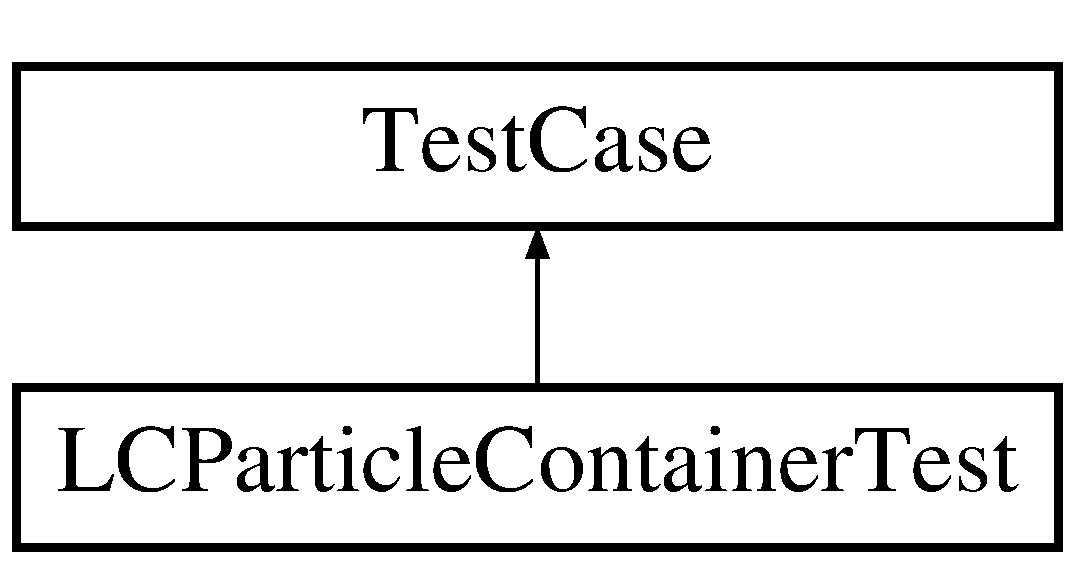
\includegraphics[height=2.000000cm]{classLCParticleContainerTest}
\end{center}
\end{figure}
\subsection*{Public Member Functions}
\begin{DoxyCompactItemize}
\item 
\hyperlink{classLCParticleContainerTest_a4380a3e7b13265e7df9c77af7a17ed5e}{L\-C\-Particle\-Container\-Test} ()
\item 
virtual \hyperlink{classLCParticleContainerTest_a505ea2563557a170d29b73efebe26e54}{$\sim$\-L\-C\-Particle\-Container\-Test} ()
\item 
void \hyperlink{classLCParticleContainerTest_ab6316e2780ff2cc8d3da231786d36e68}{set\-Up} ()
\item 
void \hyperlink{classLCParticleContainerTest_af95ad5278871f5d39305fa31def2ddc8}{tear\-Down} ()
\item 
void \hyperlink{classLCParticleContainerTest_afd02efdfde88db8256a531384bbbcfba}{test\-Initialize\-Cells} ()
\item 
void \hyperlink{classLCParticleContainerTest_a56a27be4affd57f6d765c1cde0f12e8c}{test\-Update\-Cells} ()
\item 
void \hyperlink{classLCParticleContainerTest_a334dcf062e2594cca2408c0c2713ef67}{test\-Size} ()
\item 
void \hyperlink{classLCParticleContainerTest_a29488b517572e40978e2847a7b48a64b}{test\-Begin\-Outer} ()
\item 
void \hyperlink{classLCParticleContainerTest_a46bca7862943f675190519ecb479fb16}{test\-End\-Outer} ()
\item 
void \hyperlink{classLCParticleContainerTest_a1a68785ecc6c7904ddd7d57c4184d5a8}{test\-Begin\-Inner} ()
\item 
void \hyperlink{classLCParticleContainerTest_a4c8f0fd1aac5a10fa9a6c345b3b7f15b}{test\-End\-Inner} ()
\end{DoxyCompactItemize}
\subsection*{Static Public Member Functions}
\begin{DoxyCompactItemize}
\item 
static Test $\ast$ \hyperlink{classLCParticleContainerTest_a38e97f8110510d564b91bdac41d9d9ca}{suite} ()
\end{DoxyCompactItemize}
\subsection*{Private Attributes}
\begin{DoxyCompactItemize}
\item 
\hyperlink{classutils_1_1LCParticleContainer}{utils\-::\-L\-C\-Particle\-Container} \hyperlink{classLCParticleContainerTest_aedb4bb8eb12e6079e1509ac1563c4022}{container}
\item 
int \hyperlink{classLCParticleContainerTest_a72378a90a56e81786578f90afcd41b39}{width}
\item 
int \hyperlink{classLCParticleContainerTest_a4699b4535369eb36b5d711e8b45f1da6}{height}
\item 
int \hyperlink{classLCParticleContainerTest_ab58d0d6496deca62a6452851aed96ef5}{depth}
\item 
int \hyperlink{classLCParticleContainerTest_a0d6b84232285d9630677586bb999a258}{num\-\_\-of\-\_\-cells}
\item 
double \hyperlink{classLCParticleContainerTest_a8489fd1951bb0c38acb2debd9cc5d447}{cutoff\-\_\-radius}
\item 
\hyperlink{classutils_1_1Vector}{utils\-::\-Vector}$<$ double, 3 $>$ \hyperlink{classLCParticleContainerTest_ab6450ef8318882ca6931be58e6ce58aa}{domain\-\_\-size}
\item 
std\-::list$<$ \hyperlink{classParticle}{Particle} $>$ \hyperlink{classLCParticleContainerTest_a9b0a10a86578860c76d2da5da0614e22}{particles}
\end{DoxyCompactItemize}


\subsection{Constructor \& Destructor Documentation}
\hypertarget{classLCParticleContainerTest_a4380a3e7b13265e7df9c77af7a17ed5e}{\index{L\-C\-Particle\-Container\-Test@{L\-C\-Particle\-Container\-Test}!L\-C\-Particle\-Container\-Test@{L\-C\-Particle\-Container\-Test}}
\index{L\-C\-Particle\-Container\-Test@{L\-C\-Particle\-Container\-Test}!LCParticleContainerTest@{L\-C\-Particle\-Container\-Test}}
\subsubsection[{L\-C\-Particle\-Container\-Test}]{\setlength{\rightskip}{0pt plus 5cm}L\-C\-Particle\-Container\-Test\-::\-L\-C\-Particle\-Container\-Test (
\begin{DoxyParamCaption}
{}
\end{DoxyParamCaption}
)}}\label{classLCParticleContainerTest_a4380a3e7b13265e7df9c77af7a17ed5e}
\hypertarget{classLCParticleContainerTest_a505ea2563557a170d29b73efebe26e54}{\index{L\-C\-Particle\-Container\-Test@{L\-C\-Particle\-Container\-Test}!$\sim$\-L\-C\-Particle\-Container\-Test@{$\sim$\-L\-C\-Particle\-Container\-Test}}
\index{$\sim$\-L\-C\-Particle\-Container\-Test@{$\sim$\-L\-C\-Particle\-Container\-Test}!LCParticleContainerTest@{L\-C\-Particle\-Container\-Test}}
\subsubsection[{$\sim$\-L\-C\-Particle\-Container\-Test}]{\setlength{\rightskip}{0pt plus 5cm}L\-C\-Particle\-Container\-Test\-::$\sim$\-L\-C\-Particle\-Container\-Test (
\begin{DoxyParamCaption}
{}
\end{DoxyParamCaption}
)\hspace{0.3cm}{\ttfamily [virtual]}}}\label{classLCParticleContainerTest_a505ea2563557a170d29b73efebe26e54}


\subsection{Member Function Documentation}
\hypertarget{classLCParticleContainerTest_ab6316e2780ff2cc8d3da231786d36e68}{\index{L\-C\-Particle\-Container\-Test@{L\-C\-Particle\-Container\-Test}!set\-Up@{set\-Up}}
\index{set\-Up@{set\-Up}!LCParticleContainerTest@{L\-C\-Particle\-Container\-Test}}
\subsubsection[{set\-Up}]{\setlength{\rightskip}{0pt plus 5cm}void L\-C\-Particle\-Container\-Test\-::set\-Up (
\begin{DoxyParamCaption}
{}
\end{DoxyParamCaption}
)}}\label{classLCParticleContainerTest_ab6316e2780ff2cc8d3da231786d36e68}
Set up the test variables(container, particles) \hypertarget{classLCParticleContainerTest_a38e97f8110510d564b91bdac41d9d9ca}{\index{L\-C\-Particle\-Container\-Test@{L\-C\-Particle\-Container\-Test}!suite@{suite}}
\index{suite@{suite}!LCParticleContainerTest@{L\-C\-Particle\-Container\-Test}}
\subsubsection[{suite}]{\setlength{\rightskip}{0pt plus 5cm}Cpp\-Unit\-::\-Test $\ast$ L\-C\-Particle\-Container\-Test\-::suite (
\begin{DoxyParamCaption}
{}
\end{DoxyParamCaption}
)\hspace{0.3cm}{\ttfamily [static]}}}\label{classLCParticleContainerTest_a38e97f8110510d564b91bdac41d9d9ca}
\begin{DoxyReturn}{Returns}
the Test\-Suite for the tested methods of Particle\-Container 
\end{DoxyReturn}
\hypertarget{classLCParticleContainerTest_af95ad5278871f5d39305fa31def2ddc8}{\index{L\-C\-Particle\-Container\-Test@{L\-C\-Particle\-Container\-Test}!tear\-Down@{tear\-Down}}
\index{tear\-Down@{tear\-Down}!LCParticleContainerTest@{L\-C\-Particle\-Container\-Test}}
\subsubsection[{tear\-Down}]{\setlength{\rightskip}{0pt plus 5cm}void L\-C\-Particle\-Container\-Test\-::tear\-Down (
\begin{DoxyParamCaption}
{}
\end{DoxyParamCaption}
)}}\label{classLCParticleContainerTest_af95ad5278871f5d39305fa31def2ddc8}
Tear down the test \hypertarget{classLCParticleContainerTest_a1a68785ecc6c7904ddd7d57c4184d5a8}{\index{L\-C\-Particle\-Container\-Test@{L\-C\-Particle\-Container\-Test}!test\-Begin\-Inner@{test\-Begin\-Inner}}
\index{test\-Begin\-Inner@{test\-Begin\-Inner}!LCParticleContainerTest@{L\-C\-Particle\-Container\-Test}}
\subsubsection[{test\-Begin\-Inner}]{\setlength{\rightskip}{0pt plus 5cm}void L\-C\-Particle\-Container\-Test\-::test\-Begin\-Inner (
\begin{DoxyParamCaption}
{}
\end{DoxyParamCaption}
)}}\label{classLCParticleContainerTest_a1a68785ecc6c7904ddd7d57c4184d5a8}
Check the begin\-Inner() method of the Particle\-Container \hypertarget{classLCParticleContainerTest_a29488b517572e40978e2847a7b48a64b}{\index{L\-C\-Particle\-Container\-Test@{L\-C\-Particle\-Container\-Test}!test\-Begin\-Outer@{test\-Begin\-Outer}}
\index{test\-Begin\-Outer@{test\-Begin\-Outer}!LCParticleContainerTest@{L\-C\-Particle\-Container\-Test}}
\subsubsection[{test\-Begin\-Outer}]{\setlength{\rightskip}{0pt plus 5cm}void L\-C\-Particle\-Container\-Test\-::test\-Begin\-Outer (
\begin{DoxyParamCaption}
{}
\end{DoxyParamCaption}
)}}\label{classLCParticleContainerTest_a29488b517572e40978e2847a7b48a64b}
Check the begin\-Outer() method of the Particle\-Container \hypertarget{classLCParticleContainerTest_a4c8f0fd1aac5a10fa9a6c345b3b7f15b}{\index{L\-C\-Particle\-Container\-Test@{L\-C\-Particle\-Container\-Test}!test\-End\-Inner@{test\-End\-Inner}}
\index{test\-End\-Inner@{test\-End\-Inner}!LCParticleContainerTest@{L\-C\-Particle\-Container\-Test}}
\subsubsection[{test\-End\-Inner}]{\setlength{\rightskip}{0pt plus 5cm}void L\-C\-Particle\-Container\-Test\-::test\-End\-Inner (
\begin{DoxyParamCaption}
{}
\end{DoxyParamCaption}
)}}\label{classLCParticleContainerTest_a4c8f0fd1aac5a10fa9a6c345b3b7f15b}
Check the end\-Inner() method of the Particle\-Container \hypertarget{classLCParticleContainerTest_a46bca7862943f675190519ecb479fb16}{\index{L\-C\-Particle\-Container\-Test@{L\-C\-Particle\-Container\-Test}!test\-End\-Outer@{test\-End\-Outer}}
\index{test\-End\-Outer@{test\-End\-Outer}!LCParticleContainerTest@{L\-C\-Particle\-Container\-Test}}
\subsubsection[{test\-End\-Outer}]{\setlength{\rightskip}{0pt plus 5cm}void L\-C\-Particle\-Container\-Test\-::test\-End\-Outer (
\begin{DoxyParamCaption}
{}
\end{DoxyParamCaption}
)}}\label{classLCParticleContainerTest_a46bca7862943f675190519ecb479fb16}
Check the end\-Outer() method of the Particle\-Container \hypertarget{classLCParticleContainerTest_afd02efdfde88db8256a531384bbbcfba}{\index{L\-C\-Particle\-Container\-Test@{L\-C\-Particle\-Container\-Test}!test\-Initialize\-Cells@{test\-Initialize\-Cells}}
\index{test\-Initialize\-Cells@{test\-Initialize\-Cells}!LCParticleContainerTest@{L\-C\-Particle\-Container\-Test}}
\subsubsection[{test\-Initialize\-Cells}]{\setlength{\rightskip}{0pt plus 5cm}void L\-C\-Particle\-Container\-Test\-::test\-Initialize\-Cells (
\begin{DoxyParamCaption}
{}
\end{DoxyParamCaption}
)}}\label{classLCParticleContainerTest_afd02efdfde88db8256a531384bbbcfba}
Check the initialization of the Particle\-Container \hypertarget{classLCParticleContainerTest_a334dcf062e2594cca2408c0c2713ef67}{\index{L\-C\-Particle\-Container\-Test@{L\-C\-Particle\-Container\-Test}!test\-Size@{test\-Size}}
\index{test\-Size@{test\-Size}!LCParticleContainerTest@{L\-C\-Particle\-Container\-Test}}
\subsubsection[{test\-Size}]{\setlength{\rightskip}{0pt plus 5cm}void L\-C\-Particle\-Container\-Test\-::test\-Size (
\begin{DoxyParamCaption}
{}
\end{DoxyParamCaption}
)}}\label{classLCParticleContainerTest_a334dcf062e2594cca2408c0c2713ef67}
Check the size() method of the Particle\-Container \hypertarget{classLCParticleContainerTest_a56a27be4affd57f6d765c1cde0f12e8c}{\index{L\-C\-Particle\-Container\-Test@{L\-C\-Particle\-Container\-Test}!test\-Update\-Cells@{test\-Update\-Cells}}
\index{test\-Update\-Cells@{test\-Update\-Cells}!LCParticleContainerTest@{L\-C\-Particle\-Container\-Test}}
\subsubsection[{test\-Update\-Cells}]{\setlength{\rightskip}{0pt plus 5cm}void L\-C\-Particle\-Container\-Test\-::test\-Update\-Cells (
\begin{DoxyParamCaption}
{}
\end{DoxyParamCaption}
)}}\label{classLCParticleContainerTest_a56a27be4affd57f6d765c1cde0f12e8c}
Check the update\-Cells() method of the Particle\-Container 

\subsection{Member Data Documentation}
\hypertarget{classLCParticleContainerTest_aedb4bb8eb12e6079e1509ac1563c4022}{\index{L\-C\-Particle\-Container\-Test@{L\-C\-Particle\-Container\-Test}!container@{container}}
\index{container@{container}!LCParticleContainerTest@{L\-C\-Particle\-Container\-Test}}
\subsubsection[{container}]{\setlength{\rightskip}{0pt plus 5cm}{\bf utils\-::\-L\-C\-Particle\-Container} L\-C\-Particle\-Container\-Test\-::container\hspace{0.3cm}{\ttfamily [private]}}}\label{classLCParticleContainerTest_aedb4bb8eb12e6079e1509ac1563c4022}
The particle container who will be tested \hypertarget{classLCParticleContainerTest_a8489fd1951bb0c38acb2debd9cc5d447}{\index{L\-C\-Particle\-Container\-Test@{L\-C\-Particle\-Container\-Test}!cutoff\-\_\-radius@{cutoff\-\_\-radius}}
\index{cutoff\-\_\-radius@{cutoff\-\_\-radius}!LCParticleContainerTest@{L\-C\-Particle\-Container\-Test}}
\subsubsection[{cutoff\-\_\-radius}]{\setlength{\rightskip}{0pt plus 5cm}double L\-C\-Particle\-Container\-Test\-::cutoff\-\_\-radius\hspace{0.3cm}{\ttfamily [private]}}}\label{classLCParticleContainerTest_a8489fd1951bb0c38acb2debd9cc5d447}
cutoff\-\_\-radius is the cutoff\-\_\-radius from the Lennard-\/\-Lones-\/\-Potential domain\-\_\-size is the side length of the domain \hypertarget{classLCParticleContainerTest_ab58d0d6496deca62a6452851aed96ef5}{\index{L\-C\-Particle\-Container\-Test@{L\-C\-Particle\-Container\-Test}!depth@{depth}}
\index{depth@{depth}!LCParticleContainerTest@{L\-C\-Particle\-Container\-Test}}
\subsubsection[{depth}]{\setlength{\rightskip}{0pt plus 5cm}int L\-C\-Particle\-Container\-Test\-::depth\hspace{0.3cm}{\ttfamily [private]}}}\label{classLCParticleContainerTest_ab58d0d6496deca62a6452851aed96ef5}
\hypertarget{classLCParticleContainerTest_ab6450ef8318882ca6931be58e6ce58aa}{\index{L\-C\-Particle\-Container\-Test@{L\-C\-Particle\-Container\-Test}!domain\-\_\-size@{domain\-\_\-size}}
\index{domain\-\_\-size@{domain\-\_\-size}!LCParticleContainerTest@{L\-C\-Particle\-Container\-Test}}
\subsubsection[{domain\-\_\-size}]{\setlength{\rightskip}{0pt plus 5cm}{\bf utils\-::\-Vector}$<$double, 3$>$ L\-C\-Particle\-Container\-Test\-::domain\-\_\-size\hspace{0.3cm}{\ttfamily [private]}}}\label{classLCParticleContainerTest_ab6450ef8318882ca6931be58e6ce58aa}
\hypertarget{classLCParticleContainerTest_a4699b4535369eb36b5d711e8b45f1da6}{\index{L\-C\-Particle\-Container\-Test@{L\-C\-Particle\-Container\-Test}!height@{height}}
\index{height@{height}!LCParticleContainerTest@{L\-C\-Particle\-Container\-Test}}
\subsubsection[{height}]{\setlength{\rightskip}{0pt plus 5cm}int L\-C\-Particle\-Container\-Test\-::height\hspace{0.3cm}{\ttfamily [private]}}}\label{classLCParticleContainerTest_a4699b4535369eb36b5d711e8b45f1da6}
\hypertarget{classLCParticleContainerTest_a0d6b84232285d9630677586bb999a258}{\index{L\-C\-Particle\-Container\-Test@{L\-C\-Particle\-Container\-Test}!num\-\_\-of\-\_\-cells@{num\-\_\-of\-\_\-cells}}
\index{num\-\_\-of\-\_\-cells@{num\-\_\-of\-\_\-cells}!LCParticleContainerTest@{L\-C\-Particle\-Container\-Test}}
\subsubsection[{num\-\_\-of\-\_\-cells}]{\setlength{\rightskip}{0pt plus 5cm}int L\-C\-Particle\-Container\-Test\-::num\-\_\-of\-\_\-cells\hspace{0.3cm}{\ttfamily [private]}}}\label{classLCParticleContainerTest_a0d6b84232285d9630677586bb999a258}
\hypertarget{classLCParticleContainerTest_a9b0a10a86578860c76d2da5da0614e22}{\index{L\-C\-Particle\-Container\-Test@{L\-C\-Particle\-Container\-Test}!particles@{particles}}
\index{particles@{particles}!LCParticleContainerTest@{L\-C\-Particle\-Container\-Test}}
\subsubsection[{particles}]{\setlength{\rightskip}{0pt plus 5cm}std\-::list$<${\bf Particle}$>$ L\-C\-Particle\-Container\-Test\-::particles\hspace{0.3cm}{\ttfamily [private]}}}\label{classLCParticleContainerTest_a9b0a10a86578860c76d2da5da0614e22}
The particle list, which will be used to compare to the container \hypertarget{classLCParticleContainerTest_a72378a90a56e81786578f90afcd41b39}{\index{L\-C\-Particle\-Container\-Test@{L\-C\-Particle\-Container\-Test}!width@{width}}
\index{width@{width}!LCParticleContainerTest@{L\-C\-Particle\-Container\-Test}}
\subsubsection[{width}]{\setlength{\rightskip}{0pt plus 5cm}int L\-C\-Particle\-Container\-Test\-::width\hspace{0.3cm}{\ttfamily [private]}}}\label{classLCParticleContainerTest_a72378a90a56e81786578f90afcd41b39}
width is the number of cells in x direction height is the number of cells in y direction depth is the number of cells in z direction num\-\_\-of\-\_\-cells is the total number of cells, width $\ast$ height $\ast$ depth (in case that depth is larger than 0 

The documentation for this class was generated from the following files\-:\begin{DoxyCompactItemize}
\item 
src/tests/\hyperlink{LCParticleContainerTest_8h}{L\-C\-Particle\-Container\-Test.\-h}\item 
src/tests/\hyperlink{LCParticleContainerTest_8cpp}{L\-C\-Particle\-Container\-Test.\-cpp}\end{DoxyCompactItemize}

\hypertarget{classori__t}{\section{ori\-\_\-t Class Reference}
\label{classori__t}\index{ori\-\_\-t@{ori\-\_\-t}}
}


{\ttfamily \#include $<$Input\-Cuboids.\-h$>$}

Inheritance diagram for ori\-\_\-t\-:\begin{figure}[H]
\begin{center}
\leavevmode
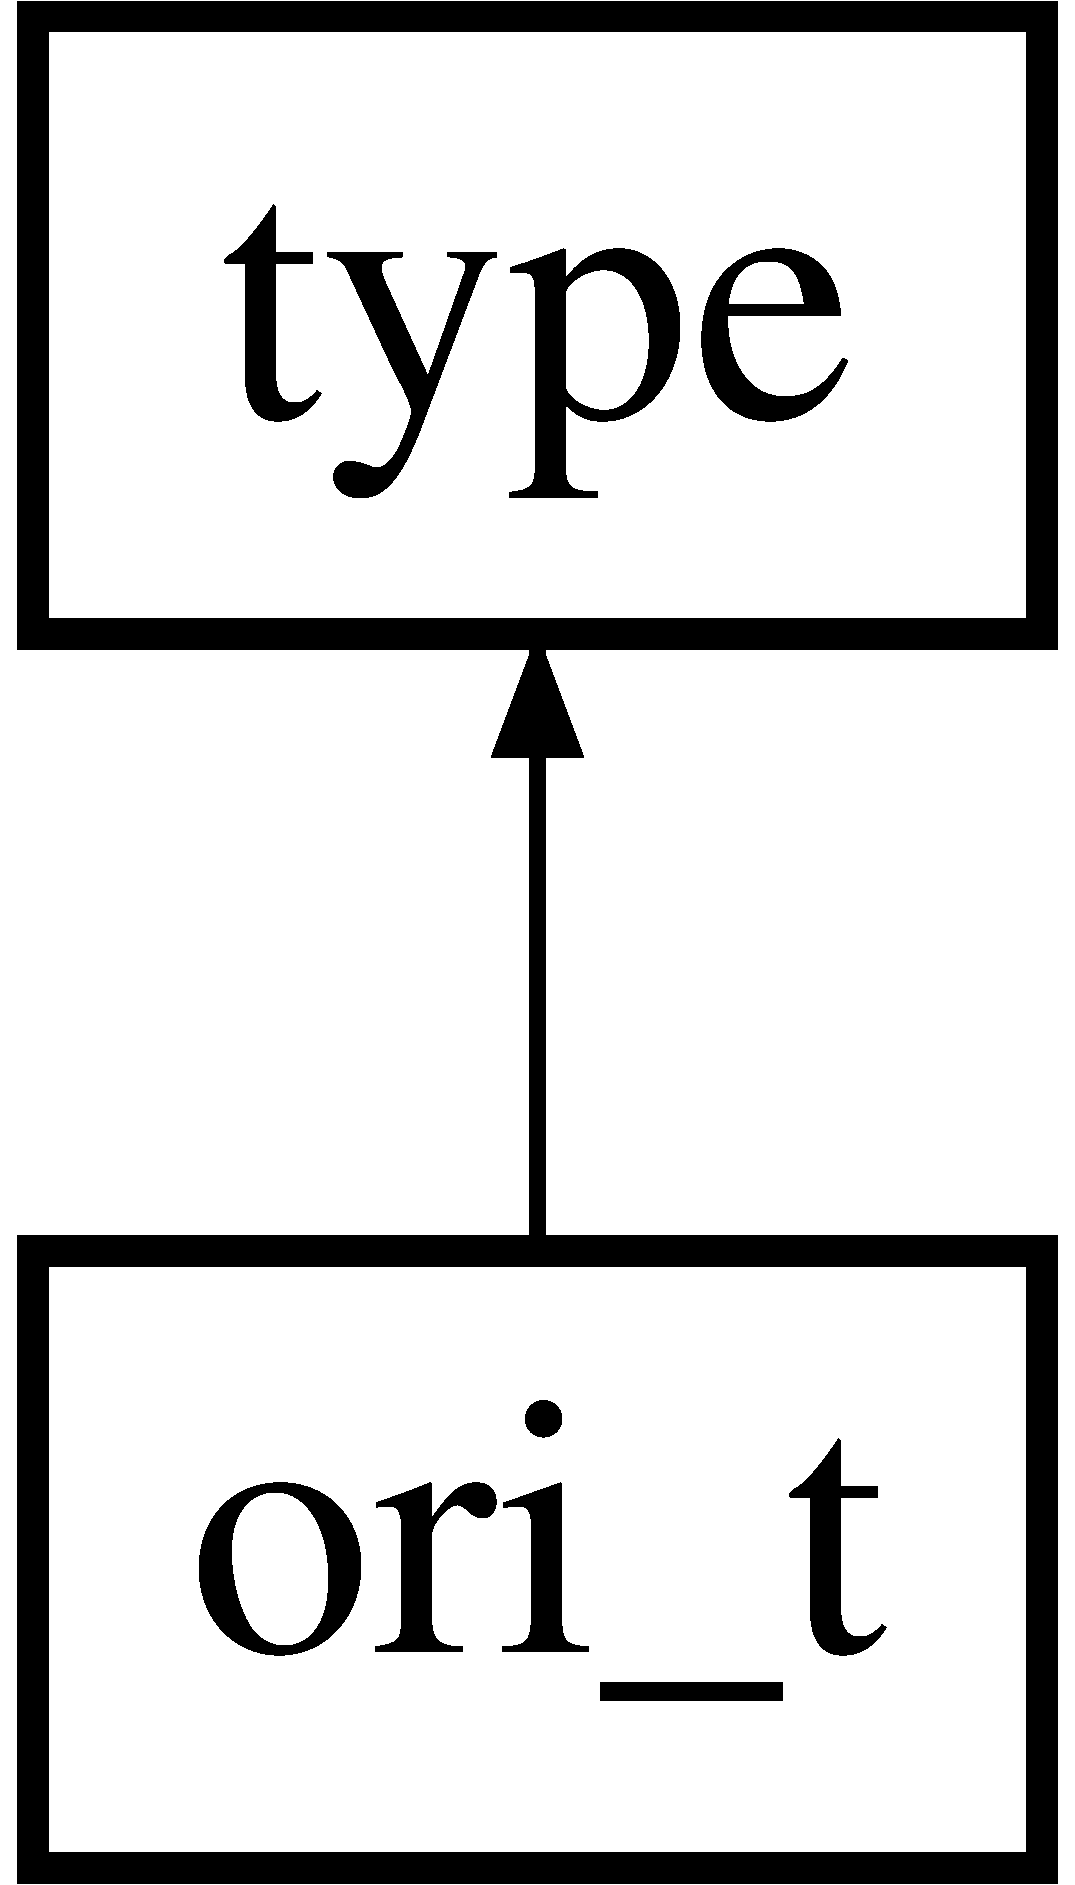
\includegraphics[height=2.000000cm]{classori__t}
\end{center}
\end{figure}
\subsection*{Public Types}
\begin{DoxyCompactItemize}
\item 
typedef \-::\hyperlink{namespacexml__schema_a69bfaf24f63a8c18ebd8e21db6b343df}{xml\-\_\-schema\-::decimal} \hyperlink{classori__t_a0d346be84e44760fbb97262b96c52110}{ori\-X\-\_\-type}
\item 
typedef \\*
\-::xsd\-::cxx\-::tree\-::traits\\*
$<$ \hyperlink{classori__t_a0d346be84e44760fbb97262b96c52110}{ori\-X\-\_\-type}, char,\-::xsd\-::cxx\-::tree\-::schema\-\_\-type\-::decimal $>$ \hyperlink{classori__t_a41d83d718921a993be9cef2cbc9b4df2}{ori\-X\-\_\-traits}
\item 
typedef \-::\hyperlink{namespacexml__schema_a69bfaf24f63a8c18ebd8e21db6b343df}{xml\-\_\-schema\-::decimal} \hyperlink{classori__t_ad04f9558bf4506128686a25e23817966}{ori\-Y\-\_\-type}
\item 
typedef \\*
\-::xsd\-::cxx\-::tree\-::traits\\*
$<$ \hyperlink{classori__t_ad04f9558bf4506128686a25e23817966}{ori\-Y\-\_\-type}, char,\-::xsd\-::cxx\-::tree\-::schema\-\_\-type\-::decimal $>$ \hyperlink{classori__t_a48bd94e6aadcf83768ddc7cf92ce5ce2}{ori\-Y\-\_\-traits}
\item 
typedef \-::\hyperlink{namespacexml__schema_a69bfaf24f63a8c18ebd8e21db6b343df}{xml\-\_\-schema\-::decimal} \hyperlink{classori__t_ade8315fb919208a45ec58303232b842b}{ori\-Z\-\_\-type}
\item 
typedef \\*
\-::xsd\-::cxx\-::tree\-::traits\\*
$<$ \hyperlink{classori__t_ade8315fb919208a45ec58303232b842b}{ori\-Z\-\_\-type}, char,\-::xsd\-::cxx\-::tree\-::schema\-\_\-type\-::decimal $>$ \hyperlink{classori__t_ad45b223f4cb199de8834bb2fcbbcbe77}{ori\-Z\-\_\-traits}
\end{DoxyCompactItemize}
\subsection*{Public Member Functions}
\begin{DoxyCompactItemize}
\item 
const \hyperlink{classori__t_a0d346be84e44760fbb97262b96c52110}{ori\-X\-\_\-type} \& \hyperlink{classori__t_ac531cde667e0a42e5142a1b6cba4d5d6}{ori\-X} () const 
\item 
\hyperlink{classori__t_a0d346be84e44760fbb97262b96c52110}{ori\-X\-\_\-type} \& \hyperlink{classori__t_aabb9fa666fe2e0c68f4f19107e31725c}{ori\-X} ()
\item 
void \hyperlink{classori__t_ad41734d912e1c04834981cbd0593736f}{ori\-X} (const \hyperlink{classori__t_a0d346be84e44760fbb97262b96c52110}{ori\-X\-\_\-type} \&x)
\item 
const \hyperlink{classori__t_ad04f9558bf4506128686a25e23817966}{ori\-Y\-\_\-type} \& \hyperlink{classori__t_a822dd139ec9b4c6fdb0dd76832cdc4b8}{ori\-Y} () const 
\item 
\hyperlink{classori__t_ad04f9558bf4506128686a25e23817966}{ori\-Y\-\_\-type} \& \hyperlink{classori__t_a570cffbf0928d39b86c715ff2e88743d}{ori\-Y} ()
\item 
void \hyperlink{classori__t_a06448162c8e97ac0373b9fc3ada36fc4}{ori\-Y} (const \hyperlink{classori__t_ad04f9558bf4506128686a25e23817966}{ori\-Y\-\_\-type} \&x)
\item 
const \hyperlink{classori__t_ade8315fb919208a45ec58303232b842b}{ori\-Z\-\_\-type} \& \hyperlink{classori__t_aa4cc5b125c6cf194c7f46f1309e9ab5c}{ori\-Z} () const 
\item 
\hyperlink{classori__t_ade8315fb919208a45ec58303232b842b}{ori\-Z\-\_\-type} \& \hyperlink{classori__t_a58e13e844f261fbd74d097377351d6ed}{ori\-Z} ()
\item 
void \hyperlink{classori__t_a3cccac2cb2c327e4cb72f2e9172a91c3}{ori\-Z} (const \hyperlink{classori__t_ade8315fb919208a45ec58303232b842b}{ori\-Z\-\_\-type} \&x)
\item 
\hyperlink{classori__t_a7005acb26895a32a12dad665fd3fd040}{ori\-\_\-t} (const \hyperlink{classori__t_a0d346be84e44760fbb97262b96c52110}{ori\-X\-\_\-type} \&, const \hyperlink{classori__t_ad04f9558bf4506128686a25e23817966}{ori\-Y\-\_\-type} \&, const \hyperlink{classori__t_ade8315fb919208a45ec58303232b842b}{ori\-Z\-\_\-type} \&)
\item 
\hyperlink{classori__t_a233c666eeeed1f06a4bf8889d0a0d790}{ori\-\_\-t} (const \-::xercesc\-::\-D\-O\-M\-Element \&e,\-::\hyperlink{namespacexml__schema_a0612287d030cb2732d31a45b258fdc87}{xml\-\_\-schema\-::flags} f=0,\-::\hyperlink{namespacexml__schema_ada9aa30dc722e93ee2ed7243085402a5}{xml\-\_\-schema\-::container} $\ast$c=0)
\item 
\hyperlink{classori__t_a72b53f599ee89c2caee595cc0966cf45}{ori\-\_\-t} (const \hyperlink{classori__t}{ori\-\_\-t} \&x,\-::\hyperlink{namespacexml__schema_a0612287d030cb2732d31a45b258fdc87}{xml\-\_\-schema\-::flags} f=0,\-::\hyperlink{namespacexml__schema_ada9aa30dc722e93ee2ed7243085402a5}{xml\-\_\-schema\-::container} $\ast$c=0)
\item 
virtual \hyperlink{classori__t}{ori\-\_\-t} $\ast$ \hyperlink{classori__t_a2d35bf90986a64146478af7232f3c72d}{\-\_\-clone} (\-::\hyperlink{namespacexml__schema_a0612287d030cb2732d31a45b258fdc87}{xml\-\_\-schema\-::flags} f=0,\-::\hyperlink{namespacexml__schema_ada9aa30dc722e93ee2ed7243085402a5}{xml\-\_\-schema\-::container} $\ast$c=0) const 
\item 
virtual \hyperlink{classori__t_a516385b1d25f706acaa19edec8a77ca3}{$\sim$ori\-\_\-t} ()
\end{DoxyCompactItemize}
\subsection*{Protected Member Functions}
\begin{DoxyCompactItemize}
\item 
void \hyperlink{classori__t_a988c7062a798e08f4c61845c0598c0c7}{parse} (\-::xsd\-::cxx\-::xml\-::dom\-::parser$<$ char $>$ \&,\-::\hyperlink{namespacexml__schema_a0612287d030cb2732d31a45b258fdc87}{xml\-\_\-schema\-::flags})
\end{DoxyCompactItemize}
\subsection*{Protected Attributes}
\begin{DoxyCompactItemize}
\item 
\-::xsd\-::cxx\-::tree\-::one$<$ \hyperlink{classori__t_a0d346be84e44760fbb97262b96c52110}{ori\-X\-\_\-type} $>$ \hyperlink{classori__t_a4b8bc23c9d2d4c4bcef1de372984b253}{ori\-X\-\_\-}
\item 
\-::xsd\-::cxx\-::tree\-::one$<$ \hyperlink{classori__t_ad04f9558bf4506128686a25e23817966}{ori\-Y\-\_\-type} $>$ \hyperlink{classori__t_a4e86990b10ec0dc34df44c3c944b30a7}{ori\-Y\-\_\-}
\item 
\-::xsd\-::cxx\-::tree\-::one$<$ \hyperlink{classori__t_ade8315fb919208a45ec58303232b842b}{ori\-Z\-\_\-type} $>$ \hyperlink{classori__t_aa9eb6ef9dc42db7707b805c8624012cb}{ori\-Z\-\_\-}
\end{DoxyCompactItemize}


\subsection{Member Typedef Documentation}
\hypertarget{classori__t_a41d83d718921a993be9cef2cbc9b4df2}{\index{ori\-\_\-t@{ori\-\_\-t}!ori\-X\-\_\-traits@{ori\-X\-\_\-traits}}
\index{ori\-X\-\_\-traits@{ori\-X\-\_\-traits}!ori_t@{ori\-\_\-t}}
\subsubsection[{ori\-X\-\_\-traits}]{\setlength{\rightskip}{0pt plus 5cm}typedef \-::xsd\-::cxx\-::tree\-::traits$<$ {\bf ori\-X\-\_\-type}, char, \-::xsd\-::cxx\-::tree\-::schema\-\_\-type\-::decimal $>$ {\bf ori\-\_\-t\-::ori\-X\-\_\-traits}}}\label{classori__t_a41d83d718921a993be9cef2cbc9b4df2}
\hypertarget{classori__t_a0d346be84e44760fbb97262b96c52110}{\index{ori\-\_\-t@{ori\-\_\-t}!ori\-X\-\_\-type@{ori\-X\-\_\-type}}
\index{ori\-X\-\_\-type@{ori\-X\-\_\-type}!ori_t@{ori\-\_\-t}}
\subsubsection[{ori\-X\-\_\-type}]{\setlength{\rightskip}{0pt plus 5cm}typedef \-::{\bf xml\-\_\-schema\-::decimal} {\bf ori\-\_\-t\-::ori\-X\-\_\-type}}}\label{classori__t_a0d346be84e44760fbb97262b96c52110}
\hypertarget{classori__t_a48bd94e6aadcf83768ddc7cf92ce5ce2}{\index{ori\-\_\-t@{ori\-\_\-t}!ori\-Y\-\_\-traits@{ori\-Y\-\_\-traits}}
\index{ori\-Y\-\_\-traits@{ori\-Y\-\_\-traits}!ori_t@{ori\-\_\-t}}
\subsubsection[{ori\-Y\-\_\-traits}]{\setlength{\rightskip}{0pt plus 5cm}typedef \-::xsd\-::cxx\-::tree\-::traits$<$ {\bf ori\-Y\-\_\-type}, char, \-::xsd\-::cxx\-::tree\-::schema\-\_\-type\-::decimal $>$ {\bf ori\-\_\-t\-::ori\-Y\-\_\-traits}}}\label{classori__t_a48bd94e6aadcf83768ddc7cf92ce5ce2}
\hypertarget{classori__t_ad04f9558bf4506128686a25e23817966}{\index{ori\-\_\-t@{ori\-\_\-t}!ori\-Y\-\_\-type@{ori\-Y\-\_\-type}}
\index{ori\-Y\-\_\-type@{ori\-Y\-\_\-type}!ori_t@{ori\-\_\-t}}
\subsubsection[{ori\-Y\-\_\-type}]{\setlength{\rightskip}{0pt plus 5cm}typedef \-::{\bf xml\-\_\-schema\-::decimal} {\bf ori\-\_\-t\-::ori\-Y\-\_\-type}}}\label{classori__t_ad04f9558bf4506128686a25e23817966}
\hypertarget{classori__t_ad45b223f4cb199de8834bb2fcbbcbe77}{\index{ori\-\_\-t@{ori\-\_\-t}!ori\-Z\-\_\-traits@{ori\-Z\-\_\-traits}}
\index{ori\-Z\-\_\-traits@{ori\-Z\-\_\-traits}!ori_t@{ori\-\_\-t}}
\subsubsection[{ori\-Z\-\_\-traits}]{\setlength{\rightskip}{0pt plus 5cm}typedef \-::xsd\-::cxx\-::tree\-::traits$<$ {\bf ori\-Z\-\_\-type}, char, \-::xsd\-::cxx\-::tree\-::schema\-\_\-type\-::decimal $>$ {\bf ori\-\_\-t\-::ori\-Z\-\_\-traits}}}\label{classori__t_ad45b223f4cb199de8834bb2fcbbcbe77}
\hypertarget{classori__t_ade8315fb919208a45ec58303232b842b}{\index{ori\-\_\-t@{ori\-\_\-t}!ori\-Z\-\_\-type@{ori\-Z\-\_\-type}}
\index{ori\-Z\-\_\-type@{ori\-Z\-\_\-type}!ori_t@{ori\-\_\-t}}
\subsubsection[{ori\-Z\-\_\-type}]{\setlength{\rightskip}{0pt plus 5cm}typedef \-::{\bf xml\-\_\-schema\-::decimal} {\bf ori\-\_\-t\-::ori\-Z\-\_\-type}}}\label{classori__t_ade8315fb919208a45ec58303232b842b}


\subsection{Constructor \& Destructor Documentation}
\hypertarget{classori__t_a7005acb26895a32a12dad665fd3fd040}{\index{ori\-\_\-t@{ori\-\_\-t}!ori\-\_\-t@{ori\-\_\-t}}
\index{ori\-\_\-t@{ori\-\_\-t}!ori_t@{ori\-\_\-t}}
\subsubsection[{ori\-\_\-t}]{\setlength{\rightskip}{0pt plus 5cm}ori\-\_\-t\-::ori\-\_\-t (
\begin{DoxyParamCaption}
\item[{const {\bf ori\-X\-\_\-type} \&}]{ori\-X, }
\item[{const {\bf ori\-Y\-\_\-type} \&}]{ori\-Y, }
\item[{const {\bf ori\-Z\-\_\-type} \&}]{ori\-Z}
\end{DoxyParamCaption}
)}}\label{classori__t_a7005acb26895a32a12dad665fd3fd040}
\hypertarget{classori__t_a233c666eeeed1f06a4bf8889d0a0d790}{\index{ori\-\_\-t@{ori\-\_\-t}!ori\-\_\-t@{ori\-\_\-t}}
\index{ori\-\_\-t@{ori\-\_\-t}!ori_t@{ori\-\_\-t}}
\subsubsection[{ori\-\_\-t}]{\setlength{\rightskip}{0pt plus 5cm}ori\-\_\-t\-::ori\-\_\-t (
\begin{DoxyParamCaption}
\item[{const \-::xercesc\-::\-D\-O\-M\-Element \&}]{e, }
\item[{\-::{\bf xml\-\_\-schema\-::flags}}]{f = {\ttfamily 0}, }
\item[{\-::{\bf xml\-\_\-schema\-::container} $\ast$}]{c = {\ttfamily 0}}
\end{DoxyParamCaption}
)}}\label{classori__t_a233c666eeeed1f06a4bf8889d0a0d790}
\hypertarget{classori__t_a72b53f599ee89c2caee595cc0966cf45}{\index{ori\-\_\-t@{ori\-\_\-t}!ori\-\_\-t@{ori\-\_\-t}}
\index{ori\-\_\-t@{ori\-\_\-t}!ori_t@{ori\-\_\-t}}
\subsubsection[{ori\-\_\-t}]{\setlength{\rightskip}{0pt plus 5cm}ori\-\_\-t\-::ori\-\_\-t (
\begin{DoxyParamCaption}
\item[{const {\bf ori\-\_\-t} \&}]{x, }
\item[{\-::{\bf xml\-\_\-schema\-::flags}}]{f = {\ttfamily 0}, }
\item[{\-::{\bf xml\-\_\-schema\-::container} $\ast$}]{c = {\ttfamily 0}}
\end{DoxyParamCaption}
)}}\label{classori__t_a72b53f599ee89c2caee595cc0966cf45}
\hypertarget{classori__t_a516385b1d25f706acaa19edec8a77ca3}{\index{ori\-\_\-t@{ori\-\_\-t}!$\sim$ori\-\_\-t@{$\sim$ori\-\_\-t}}
\index{$\sim$ori\-\_\-t@{$\sim$ori\-\_\-t}!ori_t@{ori\-\_\-t}}
\subsubsection[{$\sim$ori\-\_\-t}]{\setlength{\rightskip}{0pt plus 5cm}ori\-\_\-t\-::$\sim$ori\-\_\-t (
\begin{DoxyParamCaption}
{}
\end{DoxyParamCaption}
)\hspace{0.3cm}{\ttfamily [virtual]}}}\label{classori__t_a516385b1d25f706acaa19edec8a77ca3}


\subsection{Member Function Documentation}
\hypertarget{classori__t_a2d35bf90986a64146478af7232f3c72d}{\index{ori\-\_\-t@{ori\-\_\-t}!\-\_\-clone@{\-\_\-clone}}
\index{\-\_\-clone@{\-\_\-clone}!ori_t@{ori\-\_\-t}}
\subsubsection[{\-\_\-clone}]{\setlength{\rightskip}{0pt plus 5cm}{\bf ori\-\_\-t} $\ast$ ori\-\_\-t\-::\-\_\-clone (
\begin{DoxyParamCaption}
\item[{\-::{\bf xml\-\_\-schema\-::flags}}]{f = {\ttfamily 0}, }
\item[{\-::{\bf xml\-\_\-schema\-::container} $\ast$}]{c = {\ttfamily 0}}
\end{DoxyParamCaption}
) const\hspace{0.3cm}{\ttfamily [virtual]}}}\label{classori__t_a2d35bf90986a64146478af7232f3c72d}
\hypertarget{classori__t_ac531cde667e0a42e5142a1b6cba4d5d6}{\index{ori\-\_\-t@{ori\-\_\-t}!ori\-X@{ori\-X}}
\index{ori\-X@{ori\-X}!ori_t@{ori\-\_\-t}}
\subsubsection[{ori\-X}]{\setlength{\rightskip}{0pt plus 5cm}const {\bf ori\-\_\-t\-::ori\-X\-\_\-type} \& ori\-\_\-t\-::ori\-X (
\begin{DoxyParamCaption}
{}
\end{DoxyParamCaption}
) const}}\label{classori__t_ac531cde667e0a42e5142a1b6cba4d5d6}
\hypertarget{classori__t_aabb9fa666fe2e0c68f4f19107e31725c}{\index{ori\-\_\-t@{ori\-\_\-t}!ori\-X@{ori\-X}}
\index{ori\-X@{ori\-X}!ori_t@{ori\-\_\-t}}
\subsubsection[{ori\-X}]{\setlength{\rightskip}{0pt plus 5cm}{\bf ori\-\_\-t\-::ori\-X\-\_\-type} \& ori\-\_\-t\-::ori\-X (
\begin{DoxyParamCaption}
{}
\end{DoxyParamCaption}
)}}\label{classori__t_aabb9fa666fe2e0c68f4f19107e31725c}
\hypertarget{classori__t_ad41734d912e1c04834981cbd0593736f}{\index{ori\-\_\-t@{ori\-\_\-t}!ori\-X@{ori\-X}}
\index{ori\-X@{ori\-X}!ori_t@{ori\-\_\-t}}
\subsubsection[{ori\-X}]{\setlength{\rightskip}{0pt plus 5cm}void ori\-\_\-t\-::ori\-X (
\begin{DoxyParamCaption}
\item[{const {\bf ori\-X\-\_\-type} \&}]{x}
\end{DoxyParamCaption}
)}}\label{classori__t_ad41734d912e1c04834981cbd0593736f}
\hypertarget{classori__t_a822dd139ec9b4c6fdb0dd76832cdc4b8}{\index{ori\-\_\-t@{ori\-\_\-t}!ori\-Y@{ori\-Y}}
\index{ori\-Y@{ori\-Y}!ori_t@{ori\-\_\-t}}
\subsubsection[{ori\-Y}]{\setlength{\rightskip}{0pt plus 5cm}const {\bf ori\-\_\-t\-::ori\-Y\-\_\-type} \& ori\-\_\-t\-::ori\-Y (
\begin{DoxyParamCaption}
{}
\end{DoxyParamCaption}
) const}}\label{classori__t_a822dd139ec9b4c6fdb0dd76832cdc4b8}
\hypertarget{classori__t_a570cffbf0928d39b86c715ff2e88743d}{\index{ori\-\_\-t@{ori\-\_\-t}!ori\-Y@{ori\-Y}}
\index{ori\-Y@{ori\-Y}!ori_t@{ori\-\_\-t}}
\subsubsection[{ori\-Y}]{\setlength{\rightskip}{0pt plus 5cm}{\bf ori\-\_\-t\-::ori\-Y\-\_\-type} \& ori\-\_\-t\-::ori\-Y (
\begin{DoxyParamCaption}
{}
\end{DoxyParamCaption}
)}}\label{classori__t_a570cffbf0928d39b86c715ff2e88743d}
\hypertarget{classori__t_a06448162c8e97ac0373b9fc3ada36fc4}{\index{ori\-\_\-t@{ori\-\_\-t}!ori\-Y@{ori\-Y}}
\index{ori\-Y@{ori\-Y}!ori_t@{ori\-\_\-t}}
\subsubsection[{ori\-Y}]{\setlength{\rightskip}{0pt plus 5cm}void ori\-\_\-t\-::ori\-Y (
\begin{DoxyParamCaption}
\item[{const {\bf ori\-Y\-\_\-type} \&}]{x}
\end{DoxyParamCaption}
)}}\label{classori__t_a06448162c8e97ac0373b9fc3ada36fc4}
\hypertarget{classori__t_aa4cc5b125c6cf194c7f46f1309e9ab5c}{\index{ori\-\_\-t@{ori\-\_\-t}!ori\-Z@{ori\-Z}}
\index{ori\-Z@{ori\-Z}!ori_t@{ori\-\_\-t}}
\subsubsection[{ori\-Z}]{\setlength{\rightskip}{0pt plus 5cm}const {\bf ori\-\_\-t\-::ori\-Z\-\_\-type} \& ori\-\_\-t\-::ori\-Z (
\begin{DoxyParamCaption}
{}
\end{DoxyParamCaption}
) const}}\label{classori__t_aa4cc5b125c6cf194c7f46f1309e9ab5c}
\hypertarget{classori__t_a58e13e844f261fbd74d097377351d6ed}{\index{ori\-\_\-t@{ori\-\_\-t}!ori\-Z@{ori\-Z}}
\index{ori\-Z@{ori\-Z}!ori_t@{ori\-\_\-t}}
\subsubsection[{ori\-Z}]{\setlength{\rightskip}{0pt plus 5cm}{\bf ori\-\_\-t\-::ori\-Z\-\_\-type} \& ori\-\_\-t\-::ori\-Z (
\begin{DoxyParamCaption}
{}
\end{DoxyParamCaption}
)}}\label{classori__t_a58e13e844f261fbd74d097377351d6ed}
\hypertarget{classori__t_a3cccac2cb2c327e4cb72f2e9172a91c3}{\index{ori\-\_\-t@{ori\-\_\-t}!ori\-Z@{ori\-Z}}
\index{ori\-Z@{ori\-Z}!ori_t@{ori\-\_\-t}}
\subsubsection[{ori\-Z}]{\setlength{\rightskip}{0pt plus 5cm}void ori\-\_\-t\-::ori\-Z (
\begin{DoxyParamCaption}
\item[{const {\bf ori\-Z\-\_\-type} \&}]{x}
\end{DoxyParamCaption}
)}}\label{classori__t_a3cccac2cb2c327e4cb72f2e9172a91c3}
\hypertarget{classori__t_a988c7062a798e08f4c61845c0598c0c7}{\index{ori\-\_\-t@{ori\-\_\-t}!parse@{parse}}
\index{parse@{parse}!ori_t@{ori\-\_\-t}}
\subsubsection[{parse}]{\setlength{\rightskip}{0pt plus 5cm}void ori\-\_\-t\-::parse (
\begin{DoxyParamCaption}
\item[{\-::xsd\-::cxx\-::xml\-::dom\-::parser$<$ char $>$ \&}]{p, }
\item[{\-::{\bf xml\-\_\-schema\-::flags}}]{f}
\end{DoxyParamCaption}
)\hspace{0.3cm}{\ttfamily [protected]}}}\label{classori__t_a988c7062a798e08f4c61845c0598c0c7}


\subsection{Member Data Documentation}
\hypertarget{classori__t_a4b8bc23c9d2d4c4bcef1de372984b253}{\index{ori\-\_\-t@{ori\-\_\-t}!ori\-X\-\_\-@{ori\-X\-\_\-}}
\index{ori\-X\-\_\-@{ori\-X\-\_\-}!ori_t@{ori\-\_\-t}}
\subsubsection[{ori\-X\-\_\-}]{\setlength{\rightskip}{0pt plus 5cm}\-::xsd\-::cxx\-::tree\-::one$<$ {\bf ori\-X\-\_\-type} $>$ ori\-\_\-t\-::ori\-X\-\_\-\hspace{0.3cm}{\ttfamily [protected]}}}\label{classori__t_a4b8bc23c9d2d4c4bcef1de372984b253}
\hypertarget{classori__t_a4e86990b10ec0dc34df44c3c944b30a7}{\index{ori\-\_\-t@{ori\-\_\-t}!ori\-Y\-\_\-@{ori\-Y\-\_\-}}
\index{ori\-Y\-\_\-@{ori\-Y\-\_\-}!ori_t@{ori\-\_\-t}}
\subsubsection[{ori\-Y\-\_\-}]{\setlength{\rightskip}{0pt plus 5cm}\-::xsd\-::cxx\-::tree\-::one$<$ {\bf ori\-Y\-\_\-type} $>$ ori\-\_\-t\-::ori\-Y\-\_\-\hspace{0.3cm}{\ttfamily [protected]}}}\label{classori__t_a4e86990b10ec0dc34df44c3c944b30a7}
\hypertarget{classori__t_aa9eb6ef9dc42db7707b805c8624012cb}{\index{ori\-\_\-t@{ori\-\_\-t}!ori\-Z\-\_\-@{ori\-Z\-\_\-}}
\index{ori\-Z\-\_\-@{ori\-Z\-\_\-}!ori_t@{ori\-\_\-t}}
\subsubsection[{ori\-Z\-\_\-}]{\setlength{\rightskip}{0pt plus 5cm}\-::xsd\-::cxx\-::tree\-::one$<$ {\bf ori\-Z\-\_\-type} $>$ ori\-\_\-t\-::ori\-Z\-\_\-\hspace{0.3cm}{\ttfamily [protected]}}}\label{classori__t_aa9eb6ef9dc42db7707b805c8624012cb}


The documentation for this class was generated from the following files\-:\begin{DoxyCompactItemize}
\item 
src/utils/\hyperlink{InputCuboids_8h}{Input\-Cuboids.\-h}\item 
src/utils/\hyperlink{InputCuboids_8cpp}{Input\-Cuboids.\-cpp}\end{DoxyCompactItemize}

\hypertarget{classoutputfile__t}{\section{outputfile\-\_\-t Class Reference}
\label{classoutputfile__t}\index{outputfile\-\_\-t@{outputfile\-\_\-t}}
}


{\ttfamily \#include $<$Input\-Setting.\-h$>$}

Inheritance diagram for outputfile\-\_\-t\-:\begin{figure}[H]
\begin{center}
\leavevmode
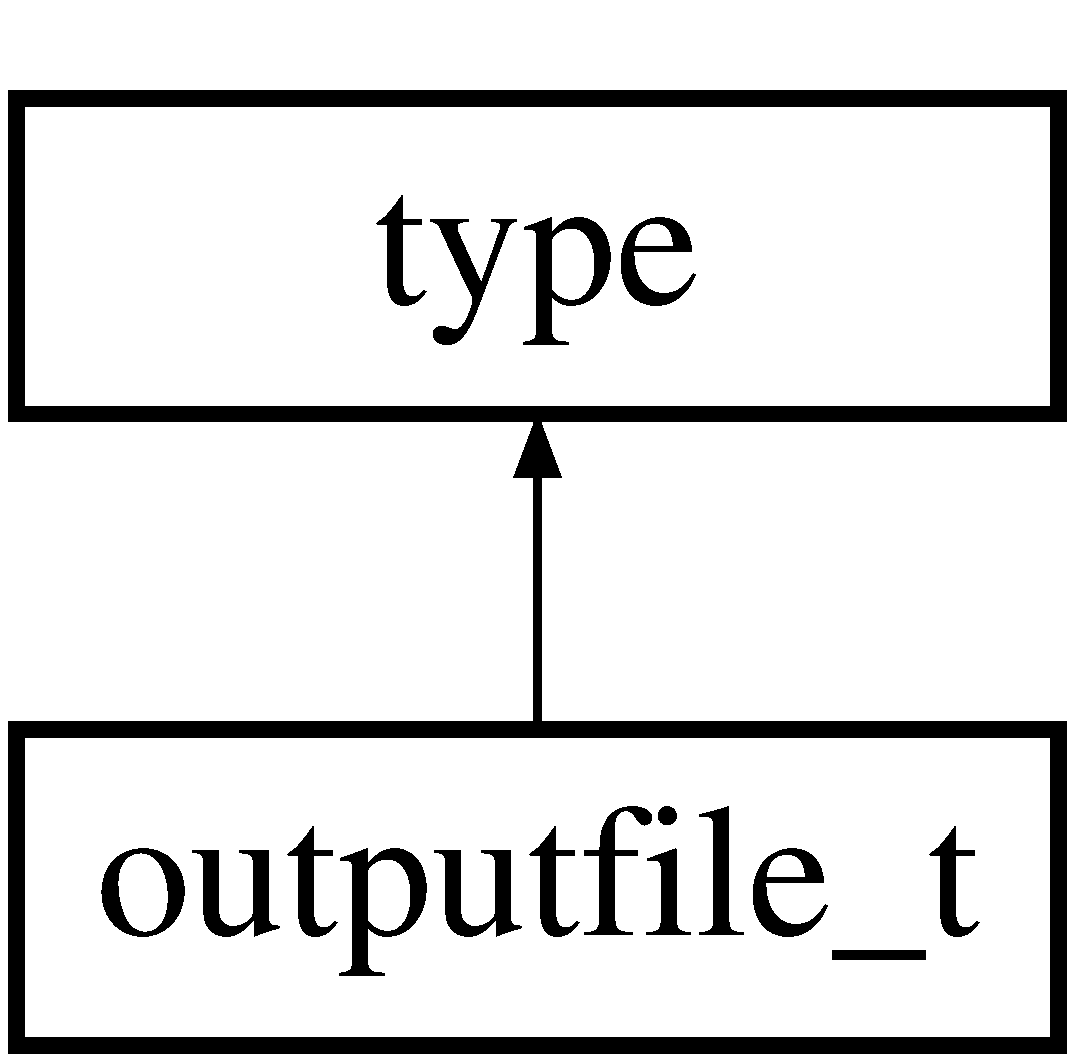
\includegraphics[height=2.000000cm]{classoutputfile__t}
\end{center}
\end{figure}
\subsection*{Public Types}
\begin{DoxyCompactItemize}
\item 
typedef \-::\hyperlink{namespacexml__schema_ac0cec83a330f0024e4e318b3deac5104}{xml\-\_\-schema\-::string} \hyperlink{classoutputfile__t_a9207f2bca21ee3d91246fae00c13d24b}{name\-\_\-type}
\item 
typedef \\*
\-::xsd\-::cxx\-::tree\-::traits\\*
$<$ \hyperlink{classoutputfile__t_a9207f2bca21ee3d91246fae00c13d24b}{name\-\_\-type}, char $>$ \hyperlink{classoutputfile__t_a8282992129b5444c95e512f7c538c1c4}{name\-\_\-traits}
\item 
typedef \-::\hyperlink{namespacexml__schema_a705720c1fed1575ccdcfd21cb7ab39ab}{xml\-\_\-schema\-::short\-\_\-} \hyperlink{classoutputfile__t_a6a45c7bbd6bb78b02c32b155fdc19dda}{freq\-\_\-type}
\item 
typedef \\*
\-::xsd\-::cxx\-::tree\-::traits\\*
$<$ \hyperlink{classoutputfile__t_a6a45c7bbd6bb78b02c32b155fdc19dda}{freq\-\_\-type}, char $>$ \hyperlink{classoutputfile__t_a04c223dc2992caa7119ac006c8ebe6d7}{freq\-\_\-traits}
\end{DoxyCompactItemize}
\subsection*{Public Member Functions}
\begin{DoxyCompactItemize}
\item 
const \hyperlink{classoutputfile__t_a9207f2bca21ee3d91246fae00c13d24b}{name\-\_\-type} \& \hyperlink{classoutputfile__t_a540932c6a4201ae883e9c699d5312c6a}{name} () const 
\item 
\hyperlink{classoutputfile__t_a9207f2bca21ee3d91246fae00c13d24b}{name\-\_\-type} \& \hyperlink{classoutputfile__t_a1247cee1df5cfbd1e9450307dd62abf2}{name} ()
\item 
void \hyperlink{classoutputfile__t_ad19c86ed66220633c4fc0392d2465ea8}{name} (const \hyperlink{classoutputfile__t_a9207f2bca21ee3d91246fae00c13d24b}{name\-\_\-type} \&x)
\item 
void \hyperlink{classoutputfile__t_a419fc94aff44d99a47412bdcba33b5b8}{name} (\-::std\-::auto\-\_\-ptr$<$ \hyperlink{classoutputfile__t_a9207f2bca21ee3d91246fae00c13d24b}{name\-\_\-type} $>$ p)
\item 
const \hyperlink{classoutputfile__t_a6a45c7bbd6bb78b02c32b155fdc19dda}{freq\-\_\-type} \& \hyperlink{classoutputfile__t_a9caa051090cab12b3c3321f33adc075d}{freq} () const 
\item 
\hyperlink{classoutputfile__t_a6a45c7bbd6bb78b02c32b155fdc19dda}{freq\-\_\-type} \& \hyperlink{classoutputfile__t_a2eb1133b18e60b957b7430839262ce0c}{freq} ()
\item 
void \hyperlink{classoutputfile__t_a39ee1f243363e6f030c652ff38483624}{freq} (const \hyperlink{classoutputfile__t_a6a45c7bbd6bb78b02c32b155fdc19dda}{freq\-\_\-type} \&x)
\item 
\hyperlink{classoutputfile__t_a920190ecdf6d02cb5fac5565b9227000}{outputfile\-\_\-t} (const \hyperlink{classoutputfile__t_a9207f2bca21ee3d91246fae00c13d24b}{name\-\_\-type} \&, const \hyperlink{classoutputfile__t_a6a45c7bbd6bb78b02c32b155fdc19dda}{freq\-\_\-type} \&)
\item 
\hyperlink{classoutputfile__t_a6b0b1fec937dd56c8adfc125c2800e95}{outputfile\-\_\-t} (const \-::xercesc\-::\-D\-O\-M\-Element \&e,\-::\hyperlink{namespacexml__schema_a0612287d030cb2732d31a45b258fdc87}{xml\-\_\-schema\-::flags} f=0,\-::\hyperlink{namespacexml__schema_ada9aa30dc722e93ee2ed7243085402a5}{xml\-\_\-schema\-::container} $\ast$c=0)
\item 
\hyperlink{classoutputfile__t_a57993b1ea7023e7aed0a37b2004a5e1c}{outputfile\-\_\-t} (const \hyperlink{classoutputfile__t}{outputfile\-\_\-t} \&x,\-::\hyperlink{namespacexml__schema_a0612287d030cb2732d31a45b258fdc87}{xml\-\_\-schema\-::flags} f=0,\-::\hyperlink{namespacexml__schema_ada9aa30dc722e93ee2ed7243085402a5}{xml\-\_\-schema\-::container} $\ast$c=0)
\item 
virtual \hyperlink{classoutputfile__t}{outputfile\-\_\-t} $\ast$ \hyperlink{classoutputfile__t_a8c602afb39c4ce44f0b7604f83e4ccb3}{\-\_\-clone} (\-::\hyperlink{namespacexml__schema_a0612287d030cb2732d31a45b258fdc87}{xml\-\_\-schema\-::flags} f=0,\-::\hyperlink{namespacexml__schema_ada9aa30dc722e93ee2ed7243085402a5}{xml\-\_\-schema\-::container} $\ast$c=0) const 
\item 
virtual \hyperlink{classoutputfile__t_a746eb3e22698d25bb5c13cb4b138fc08}{$\sim$outputfile\-\_\-t} ()
\end{DoxyCompactItemize}
\subsection*{Protected Member Functions}
\begin{DoxyCompactItemize}
\item 
void \hyperlink{classoutputfile__t_a1d428888cb0aa643c8c02865c883a595}{parse} (\-::xsd\-::cxx\-::xml\-::dom\-::parser$<$ char $>$ \&,\-::\hyperlink{namespacexml__schema_a0612287d030cb2732d31a45b258fdc87}{xml\-\_\-schema\-::flags})
\end{DoxyCompactItemize}
\subsection*{Protected Attributes}
\begin{DoxyCompactItemize}
\item 
\-::xsd\-::cxx\-::tree\-::one$<$ \hyperlink{classoutputfile__t_a9207f2bca21ee3d91246fae00c13d24b}{name\-\_\-type} $>$ \hyperlink{classoutputfile__t_a593a1f4fb1a7e2c1f9cace3a5fc9bc11}{name\-\_\-}
\item 
\-::xsd\-::cxx\-::tree\-::one$<$ \hyperlink{classoutputfile__t_a6a45c7bbd6bb78b02c32b155fdc19dda}{freq\-\_\-type} $>$ \hyperlink{classoutputfile__t_a7d4cbfeeb02491ef8dfe4df991e3e85f}{freq\-\_\-}
\end{DoxyCompactItemize}


\subsection{Member Typedef Documentation}
\hypertarget{classoutputfile__t_a04c223dc2992caa7119ac006c8ebe6d7}{\index{outputfile\-\_\-t@{outputfile\-\_\-t}!freq\-\_\-traits@{freq\-\_\-traits}}
\index{freq\-\_\-traits@{freq\-\_\-traits}!outputfile_t@{outputfile\-\_\-t}}
\subsubsection[{freq\-\_\-traits}]{\setlength{\rightskip}{0pt plus 5cm}typedef \-::xsd\-::cxx\-::tree\-::traits$<$ {\bf freq\-\_\-type}, char $>$ {\bf outputfile\-\_\-t\-::freq\-\_\-traits}}}\label{classoutputfile__t_a04c223dc2992caa7119ac006c8ebe6d7}
\hypertarget{classoutputfile__t_a6a45c7bbd6bb78b02c32b155fdc19dda}{\index{outputfile\-\_\-t@{outputfile\-\_\-t}!freq\-\_\-type@{freq\-\_\-type}}
\index{freq\-\_\-type@{freq\-\_\-type}!outputfile_t@{outputfile\-\_\-t}}
\subsubsection[{freq\-\_\-type}]{\setlength{\rightskip}{0pt plus 5cm}typedef \-::{\bf xml\-\_\-schema\-::short\-\_\-} {\bf outputfile\-\_\-t\-::freq\-\_\-type}}}\label{classoutputfile__t_a6a45c7bbd6bb78b02c32b155fdc19dda}
\hypertarget{classoutputfile__t_a8282992129b5444c95e512f7c538c1c4}{\index{outputfile\-\_\-t@{outputfile\-\_\-t}!name\-\_\-traits@{name\-\_\-traits}}
\index{name\-\_\-traits@{name\-\_\-traits}!outputfile_t@{outputfile\-\_\-t}}
\subsubsection[{name\-\_\-traits}]{\setlength{\rightskip}{0pt plus 5cm}typedef \-::xsd\-::cxx\-::tree\-::traits$<$ {\bf name\-\_\-type}, char $>$ {\bf outputfile\-\_\-t\-::name\-\_\-traits}}}\label{classoutputfile__t_a8282992129b5444c95e512f7c538c1c4}
\hypertarget{classoutputfile__t_a9207f2bca21ee3d91246fae00c13d24b}{\index{outputfile\-\_\-t@{outputfile\-\_\-t}!name\-\_\-type@{name\-\_\-type}}
\index{name\-\_\-type@{name\-\_\-type}!outputfile_t@{outputfile\-\_\-t}}
\subsubsection[{name\-\_\-type}]{\setlength{\rightskip}{0pt plus 5cm}typedef \-::{\bf xml\-\_\-schema\-::string} {\bf outputfile\-\_\-t\-::name\-\_\-type}}}\label{classoutputfile__t_a9207f2bca21ee3d91246fae00c13d24b}


\subsection{Constructor \& Destructor Documentation}
\hypertarget{classoutputfile__t_a920190ecdf6d02cb5fac5565b9227000}{\index{outputfile\-\_\-t@{outputfile\-\_\-t}!outputfile\-\_\-t@{outputfile\-\_\-t}}
\index{outputfile\-\_\-t@{outputfile\-\_\-t}!outputfile_t@{outputfile\-\_\-t}}
\subsubsection[{outputfile\-\_\-t}]{\setlength{\rightskip}{0pt plus 5cm}outputfile\-\_\-t\-::outputfile\-\_\-t (
\begin{DoxyParamCaption}
\item[{const {\bf name\-\_\-type} \&}]{name, }
\item[{const {\bf freq\-\_\-type} \&}]{freq}
\end{DoxyParamCaption}
)}}\label{classoutputfile__t_a920190ecdf6d02cb5fac5565b9227000}
\hypertarget{classoutputfile__t_a6b0b1fec937dd56c8adfc125c2800e95}{\index{outputfile\-\_\-t@{outputfile\-\_\-t}!outputfile\-\_\-t@{outputfile\-\_\-t}}
\index{outputfile\-\_\-t@{outputfile\-\_\-t}!outputfile_t@{outputfile\-\_\-t}}
\subsubsection[{outputfile\-\_\-t}]{\setlength{\rightskip}{0pt plus 5cm}outputfile\-\_\-t\-::outputfile\-\_\-t (
\begin{DoxyParamCaption}
\item[{const \-::xercesc\-::\-D\-O\-M\-Element \&}]{e, }
\item[{\-::{\bf xml\-\_\-schema\-::flags}}]{f = {\ttfamily 0}, }
\item[{\-::{\bf xml\-\_\-schema\-::container} $\ast$}]{c = {\ttfamily 0}}
\end{DoxyParamCaption}
)}}\label{classoutputfile__t_a6b0b1fec937dd56c8adfc125c2800e95}
\hypertarget{classoutputfile__t_a57993b1ea7023e7aed0a37b2004a5e1c}{\index{outputfile\-\_\-t@{outputfile\-\_\-t}!outputfile\-\_\-t@{outputfile\-\_\-t}}
\index{outputfile\-\_\-t@{outputfile\-\_\-t}!outputfile_t@{outputfile\-\_\-t}}
\subsubsection[{outputfile\-\_\-t}]{\setlength{\rightskip}{0pt plus 5cm}outputfile\-\_\-t\-::outputfile\-\_\-t (
\begin{DoxyParamCaption}
\item[{const {\bf outputfile\-\_\-t} \&}]{x, }
\item[{\-::{\bf xml\-\_\-schema\-::flags}}]{f = {\ttfamily 0}, }
\item[{\-::{\bf xml\-\_\-schema\-::container} $\ast$}]{c = {\ttfamily 0}}
\end{DoxyParamCaption}
)}}\label{classoutputfile__t_a57993b1ea7023e7aed0a37b2004a5e1c}
\hypertarget{classoutputfile__t_a746eb3e22698d25bb5c13cb4b138fc08}{\index{outputfile\-\_\-t@{outputfile\-\_\-t}!$\sim$outputfile\-\_\-t@{$\sim$outputfile\-\_\-t}}
\index{$\sim$outputfile\-\_\-t@{$\sim$outputfile\-\_\-t}!outputfile_t@{outputfile\-\_\-t}}
\subsubsection[{$\sim$outputfile\-\_\-t}]{\setlength{\rightskip}{0pt plus 5cm}outputfile\-\_\-t\-::$\sim$outputfile\-\_\-t (
\begin{DoxyParamCaption}
{}
\end{DoxyParamCaption}
)\hspace{0.3cm}{\ttfamily [virtual]}}}\label{classoutputfile__t_a746eb3e22698d25bb5c13cb4b138fc08}


\subsection{Member Function Documentation}
\hypertarget{classoutputfile__t_a8c602afb39c4ce44f0b7604f83e4ccb3}{\index{outputfile\-\_\-t@{outputfile\-\_\-t}!\-\_\-clone@{\-\_\-clone}}
\index{\-\_\-clone@{\-\_\-clone}!outputfile_t@{outputfile\-\_\-t}}
\subsubsection[{\-\_\-clone}]{\setlength{\rightskip}{0pt plus 5cm}{\bf outputfile\-\_\-t} $\ast$ outputfile\-\_\-t\-::\-\_\-clone (
\begin{DoxyParamCaption}
\item[{\-::{\bf xml\-\_\-schema\-::flags}}]{f = {\ttfamily 0}, }
\item[{\-::{\bf xml\-\_\-schema\-::container} $\ast$}]{c = {\ttfamily 0}}
\end{DoxyParamCaption}
) const\hspace{0.3cm}{\ttfamily [virtual]}}}\label{classoutputfile__t_a8c602afb39c4ce44f0b7604f83e4ccb3}
\hypertarget{classoutputfile__t_a9caa051090cab12b3c3321f33adc075d}{\index{outputfile\-\_\-t@{outputfile\-\_\-t}!freq@{freq}}
\index{freq@{freq}!outputfile_t@{outputfile\-\_\-t}}
\subsubsection[{freq}]{\setlength{\rightskip}{0pt plus 5cm}const {\bf outputfile\-\_\-t\-::freq\-\_\-type} \& outputfile\-\_\-t\-::freq (
\begin{DoxyParamCaption}
{}
\end{DoxyParamCaption}
) const}}\label{classoutputfile__t_a9caa051090cab12b3c3321f33adc075d}
\hypertarget{classoutputfile__t_a2eb1133b18e60b957b7430839262ce0c}{\index{outputfile\-\_\-t@{outputfile\-\_\-t}!freq@{freq}}
\index{freq@{freq}!outputfile_t@{outputfile\-\_\-t}}
\subsubsection[{freq}]{\setlength{\rightskip}{0pt plus 5cm}{\bf outputfile\-\_\-t\-::freq\-\_\-type} \& outputfile\-\_\-t\-::freq (
\begin{DoxyParamCaption}
{}
\end{DoxyParamCaption}
)}}\label{classoutputfile__t_a2eb1133b18e60b957b7430839262ce0c}
\hypertarget{classoutputfile__t_a39ee1f243363e6f030c652ff38483624}{\index{outputfile\-\_\-t@{outputfile\-\_\-t}!freq@{freq}}
\index{freq@{freq}!outputfile_t@{outputfile\-\_\-t}}
\subsubsection[{freq}]{\setlength{\rightskip}{0pt plus 5cm}void outputfile\-\_\-t\-::freq (
\begin{DoxyParamCaption}
\item[{const {\bf freq\-\_\-type} \&}]{x}
\end{DoxyParamCaption}
)}}\label{classoutputfile__t_a39ee1f243363e6f030c652ff38483624}
\hypertarget{classoutputfile__t_a540932c6a4201ae883e9c699d5312c6a}{\index{outputfile\-\_\-t@{outputfile\-\_\-t}!name@{name}}
\index{name@{name}!outputfile_t@{outputfile\-\_\-t}}
\subsubsection[{name}]{\setlength{\rightskip}{0pt plus 5cm}const {\bf outputfile\-\_\-t\-::name\-\_\-type} \& outputfile\-\_\-t\-::name (
\begin{DoxyParamCaption}
{}
\end{DoxyParamCaption}
) const}}\label{classoutputfile__t_a540932c6a4201ae883e9c699d5312c6a}
\hypertarget{classoutputfile__t_a1247cee1df5cfbd1e9450307dd62abf2}{\index{outputfile\-\_\-t@{outputfile\-\_\-t}!name@{name}}
\index{name@{name}!outputfile_t@{outputfile\-\_\-t}}
\subsubsection[{name}]{\setlength{\rightskip}{0pt plus 5cm}{\bf outputfile\-\_\-t\-::name\-\_\-type} \& outputfile\-\_\-t\-::name (
\begin{DoxyParamCaption}
{}
\end{DoxyParamCaption}
)}}\label{classoutputfile__t_a1247cee1df5cfbd1e9450307dd62abf2}
\hypertarget{classoutputfile__t_ad19c86ed66220633c4fc0392d2465ea8}{\index{outputfile\-\_\-t@{outputfile\-\_\-t}!name@{name}}
\index{name@{name}!outputfile_t@{outputfile\-\_\-t}}
\subsubsection[{name}]{\setlength{\rightskip}{0pt plus 5cm}void outputfile\-\_\-t\-::name (
\begin{DoxyParamCaption}
\item[{const {\bf name\-\_\-type} \&}]{x}
\end{DoxyParamCaption}
)}}\label{classoutputfile__t_ad19c86ed66220633c4fc0392d2465ea8}
\hypertarget{classoutputfile__t_a419fc94aff44d99a47412bdcba33b5b8}{\index{outputfile\-\_\-t@{outputfile\-\_\-t}!name@{name}}
\index{name@{name}!outputfile_t@{outputfile\-\_\-t}}
\subsubsection[{name}]{\setlength{\rightskip}{0pt plus 5cm}void outputfile\-\_\-t\-::name (
\begin{DoxyParamCaption}
\item[{\-::std\-::auto\-\_\-ptr$<$ {\bf name\-\_\-type} $>$}]{p}
\end{DoxyParamCaption}
)}}\label{classoutputfile__t_a419fc94aff44d99a47412bdcba33b5b8}
\hypertarget{classoutputfile__t_a1d428888cb0aa643c8c02865c883a595}{\index{outputfile\-\_\-t@{outputfile\-\_\-t}!parse@{parse}}
\index{parse@{parse}!outputfile_t@{outputfile\-\_\-t}}
\subsubsection[{parse}]{\setlength{\rightskip}{0pt plus 5cm}void outputfile\-\_\-t\-::parse (
\begin{DoxyParamCaption}
\item[{\-::xsd\-::cxx\-::xml\-::dom\-::parser$<$ char $>$ \&}]{p, }
\item[{\-::{\bf xml\-\_\-schema\-::flags}}]{f}
\end{DoxyParamCaption}
)\hspace{0.3cm}{\ttfamily [protected]}}}\label{classoutputfile__t_a1d428888cb0aa643c8c02865c883a595}


\subsection{Member Data Documentation}
\hypertarget{classoutputfile__t_a7d4cbfeeb02491ef8dfe4df991e3e85f}{\index{outputfile\-\_\-t@{outputfile\-\_\-t}!freq\-\_\-@{freq\-\_\-}}
\index{freq\-\_\-@{freq\-\_\-}!outputfile_t@{outputfile\-\_\-t}}
\subsubsection[{freq\-\_\-}]{\setlength{\rightskip}{0pt plus 5cm}\-::xsd\-::cxx\-::tree\-::one$<$ {\bf freq\-\_\-type} $>$ outputfile\-\_\-t\-::freq\-\_\-\hspace{0.3cm}{\ttfamily [protected]}}}\label{classoutputfile__t_a7d4cbfeeb02491ef8dfe4df991e3e85f}
\hypertarget{classoutputfile__t_a593a1f4fb1a7e2c1f9cace3a5fc9bc11}{\index{outputfile\-\_\-t@{outputfile\-\_\-t}!name\-\_\-@{name\-\_\-}}
\index{name\-\_\-@{name\-\_\-}!outputfile_t@{outputfile\-\_\-t}}
\subsubsection[{name\-\_\-}]{\setlength{\rightskip}{0pt plus 5cm}\-::xsd\-::cxx\-::tree\-::one$<$ {\bf name\-\_\-type} $>$ outputfile\-\_\-t\-::name\-\_\-\hspace{0.3cm}{\ttfamily [protected]}}}\label{classoutputfile__t_a593a1f4fb1a7e2c1f9cace3a5fc9bc11}


The documentation for this class was generated from the following files\-:\begin{DoxyCompactItemize}
\item 
src/utils/\hyperlink{InputSetting_8h}{Input\-Setting.\-h}\item 
src/utils/\hyperlink{InputSetting_8cpp}{Input\-Setting.\-cpp}\end{DoxyCompactItemize}

\hypertarget{classParticle}{\section{Particle Class Reference}
\label{classParticle}\index{Particle@{Particle}}
}


{\ttfamily \#include $<$Particle.\-h$>$}

\subsection*{Public Member Functions}
\begin{DoxyCompactItemize}
\item 
\hyperlink{classParticle_a866812d3dfb9c539e5e24593e596a8c9}{Particle} (int \hyperlink{classtype}{type}=0)
\item 
\hyperlink{classParticle_a24b04cb7c6f7ea4242d25c410f44ae56}{Particle} (const \hyperlink{classParticle}{Particle} \&other)
\item 
\hyperlink{classParticle_ab1cd2d4c36a52cb9ea5755340aceafe0}{Particle} (\hyperlink{classutils_1_1Vector}{utils\-::\-Vector}$<$ double, 3 $>$ x\-\_\-arg, \hyperlink{classutils_1_1Vector}{utils\-::\-Vector}$<$ double, 3 $>$ v\-\_\-arg, double m\-\_\-arg, int \hyperlink{classtype}{type})
\item 
virtual \hyperlink{classParticle_ad030d0fe7b88cf81744b127c99244ff4}{$\sim$\-Particle} ()
\item 
\hyperlink{classutils_1_1Vector}{utils\-::\-Vector}$<$ double, 3 $>$ \& \hyperlink{classParticle_ab7ade5dc156dfa0234aa0323564e46ed}{get\-X} ()
\item 
\hyperlink{classutils_1_1Vector}{utils\-::\-Vector}$<$ double, 3 $>$ \& \hyperlink{classParticle_acd84c445e2bd5f5280a00e76cfe73fe0}{get\-F} ()
\item 
\hyperlink{classutils_1_1Vector}{utils\-::\-Vector}$<$ double, 3 $>$ \& \hyperlink{classParticle_a1204435fc08c697b0fea230616d1bbdf}{get\-Old\-F} ()
\item 
\hyperlink{classutils_1_1Vector}{utils\-::\-Vector}$<$ double, 3 $>$ \& \hyperlink{classParticle_aaf3ecbc6e1e31b259fe239461ba13dbd}{get\-V} ()
\item 
\hyperlink{classutils_1_1Vector}{utils\-::\-Vector}$<$ double, 3 $>$ \hyperlink{classParticle_aab82b05d8e3be6f085430e0b8b957eaa}{get\-Temp\-F} ()
\item 
double \& \hyperlink{classParticle_a88ac76c41c96b8df6de3e0bc14edbbc8}{get\-M} ()
\item 
int \& \hyperlink{classParticle_abf02d7c78c7d9c1944a066816f9a7139}{get\-Type} ()
\item 
bool \hyperlink{classParticle_a5034babb77618a56e00927d8891afabe}{operator==} (\hyperlink{classParticle}{Particle} \&other)
\item 
std\-::string \hyperlink{classParticle_a07d071a0f91f8ce7413201a6db3afe7b}{to\-String} ()
\item 
void \hyperlink{classParticle_ae86d7fda94283bde380ea261333d8ac6}{set\-F} (\hyperlink{classutils_1_1Vector}{utils\-::\-Vector}$<$ double, 3 $>$ new\-F)
\item 
void \hyperlink{classParticle_ad467aec6031c428df7670ba5c7af9e28}{delete\-Temp\-F} ()
\item 
void \hyperlink{classParticle_ac7b9564f3f7ef87940216f9021cb5f61}{update\-Temp\-F} (\hyperlink{classutils_1_1Vector}{utils\-::\-Vector}$<$ double, 3 $>$ new\-F)
\end{DoxyCompactItemize}
\subsection*{Private Attributes}
\begin{DoxyCompactItemize}
\item 
\hyperlink{classutils_1_1Vector}{utils\-::\-Vector}$<$ double, 3 $>$ \hyperlink{classParticle_a3789900d6fe19a75d3a82cd5e9622c4c}{x}
\item 
\hyperlink{classutils_1_1Vector}{utils\-::\-Vector}$<$ double, 3 $>$ \hyperlink{classParticle_ac3669e50d83d8608d522965b9acd1d8b}{v}
\item 
\hyperlink{classutils_1_1Vector}{utils\-::\-Vector}$<$ double, 3 $>$ \hyperlink{classParticle_ad9aa3e171ea950b2cff1b4825e67845b}{f}
\item 
\hyperlink{classutils_1_1Vector}{utils\-::\-Vector}$<$ double, 3 $>$ \hyperlink{classParticle_aef8faa875660fc5da7392d577af9d419}{temp\-\_\-f}
\item 
\hyperlink{classutils_1_1Vector}{utils\-::\-Vector}$<$ double, 3 $>$ \hyperlink{classParticle_ad9281e33474f23f7261f28848affc4a4}{old\-\_\-f}
\item 
double \hyperlink{classParticle_aedcc7e1bc53b0e2b1a4a07c9a1b47563}{m}
\item 
int \hyperlink{classParticle_a2b73dd42bcd56ba2e7ffeb0a5515a866}{type}
\end{DoxyCompactItemize}


\subsection{Constructor \& Destructor Documentation}
\hypertarget{classParticle_a866812d3dfb9c539e5e24593e596a8c9}{\index{Particle@{Particle}!Particle@{Particle}}
\index{Particle@{Particle}!Particle@{Particle}}
\subsubsection[{Particle}]{\setlength{\rightskip}{0pt plus 5cm}Particle\-::\-Particle (
\begin{DoxyParamCaption}
\item[{int}]{type = {\ttfamily 0}}
\end{DoxyParamCaption}
)}}\label{classParticle_a866812d3dfb9c539e5e24593e596a8c9}
\hypertarget{classParticle_a24b04cb7c6f7ea4242d25c410f44ae56}{\index{Particle@{Particle}!Particle@{Particle}}
\index{Particle@{Particle}!Particle@{Particle}}
\subsubsection[{Particle}]{\setlength{\rightskip}{0pt plus 5cm}Particle\-::\-Particle (
\begin{DoxyParamCaption}
\item[{const {\bf Particle} \&}]{other}
\end{DoxyParamCaption}
)}}\label{classParticle_a24b04cb7c6f7ea4242d25c410f44ae56}
\hypertarget{classParticle_ab1cd2d4c36a52cb9ea5755340aceafe0}{\index{Particle@{Particle}!Particle@{Particle}}
\index{Particle@{Particle}!Particle@{Particle}}
\subsubsection[{Particle}]{\setlength{\rightskip}{0pt plus 5cm}Particle\-::\-Particle (
\begin{DoxyParamCaption}
\item[{{\bf utils\-::\-Vector}$<$ double, 3 $>$}]{x\-\_\-arg, }
\item[{{\bf utils\-::\-Vector}$<$ double, 3 $>$}]{v\-\_\-arg, }
\item[{double}]{m\-\_\-arg, }
\item[{int}]{type}
\end{DoxyParamCaption}
)}}\label{classParticle_ab1cd2d4c36a52cb9ea5755340aceafe0}
\hypertarget{classParticle_ad030d0fe7b88cf81744b127c99244ff4}{\index{Particle@{Particle}!$\sim$\-Particle@{$\sim$\-Particle}}
\index{$\sim$\-Particle@{$\sim$\-Particle}!Particle@{Particle}}
\subsubsection[{$\sim$\-Particle}]{\setlength{\rightskip}{0pt plus 5cm}Particle\-::$\sim$\-Particle (
\begin{DoxyParamCaption}
{}
\end{DoxyParamCaption}
)\hspace{0.3cm}{\ttfamily [virtual]}}}\label{classParticle_ad030d0fe7b88cf81744b127c99244ff4}


\subsection{Member Function Documentation}
\hypertarget{classParticle_ad467aec6031c428df7670ba5c7af9e28}{\index{Particle@{Particle}!delete\-Temp\-F@{delete\-Temp\-F}}
\index{delete\-Temp\-F@{delete\-Temp\-F}!Particle@{Particle}}
\subsubsection[{delete\-Temp\-F}]{\setlength{\rightskip}{0pt plus 5cm}void Particle\-::delete\-Temp\-F (
\begin{DoxyParamCaption}
{}
\end{DoxyParamCaption}
)}}\label{classParticle_ad467aec6031c428df7670ba5c7af9e28}
\hypertarget{classParticle_acd84c445e2bd5f5280a00e76cfe73fe0}{\index{Particle@{Particle}!get\-F@{get\-F}}
\index{get\-F@{get\-F}!Particle@{Particle}}
\subsubsection[{get\-F}]{\setlength{\rightskip}{0pt plus 5cm}{\bf utils\-::\-Vector}$<$ double, 3 $>$ \& Particle\-::get\-F (
\begin{DoxyParamCaption}
{}
\end{DoxyParamCaption}
)}}\label{classParticle_acd84c445e2bd5f5280a00e76cfe73fe0}
\hypertarget{classParticle_a88ac76c41c96b8df6de3e0bc14edbbc8}{\index{Particle@{Particle}!get\-M@{get\-M}}
\index{get\-M@{get\-M}!Particle@{Particle}}
\subsubsection[{get\-M}]{\setlength{\rightskip}{0pt plus 5cm}double \& Particle\-::get\-M (
\begin{DoxyParamCaption}
{}
\end{DoxyParamCaption}
)}}\label{classParticle_a88ac76c41c96b8df6de3e0bc14edbbc8}
\hypertarget{classParticle_a1204435fc08c697b0fea230616d1bbdf}{\index{Particle@{Particle}!get\-Old\-F@{get\-Old\-F}}
\index{get\-Old\-F@{get\-Old\-F}!Particle@{Particle}}
\subsubsection[{get\-Old\-F}]{\setlength{\rightskip}{0pt plus 5cm}{\bf utils\-::\-Vector}$<$ double, 3 $>$ \& Particle\-::get\-Old\-F (
\begin{DoxyParamCaption}
{}
\end{DoxyParamCaption}
)}}\label{classParticle_a1204435fc08c697b0fea230616d1bbdf}
\hypertarget{classParticle_aab82b05d8e3be6f085430e0b8b957eaa}{\index{Particle@{Particle}!get\-Temp\-F@{get\-Temp\-F}}
\index{get\-Temp\-F@{get\-Temp\-F}!Particle@{Particle}}
\subsubsection[{get\-Temp\-F}]{\setlength{\rightskip}{0pt plus 5cm}{\bf utils\-::\-Vector}$<$ double, 3 $>$ Particle\-::get\-Temp\-F (
\begin{DoxyParamCaption}
{}
\end{DoxyParamCaption}
)}}\label{classParticle_aab82b05d8e3be6f085430e0b8b957eaa}
\hypertarget{classParticle_abf02d7c78c7d9c1944a066816f9a7139}{\index{Particle@{Particle}!get\-Type@{get\-Type}}
\index{get\-Type@{get\-Type}!Particle@{Particle}}
\subsubsection[{get\-Type}]{\setlength{\rightskip}{0pt plus 5cm}int \& Particle\-::get\-Type (
\begin{DoxyParamCaption}
{}
\end{DoxyParamCaption}
)}}\label{classParticle_abf02d7c78c7d9c1944a066816f9a7139}
\hypertarget{classParticle_aaf3ecbc6e1e31b259fe239461ba13dbd}{\index{Particle@{Particle}!get\-V@{get\-V}}
\index{get\-V@{get\-V}!Particle@{Particle}}
\subsubsection[{get\-V}]{\setlength{\rightskip}{0pt plus 5cm}{\bf utils\-::\-Vector}$<$ double, 3 $>$ \& Particle\-::get\-V (
\begin{DoxyParamCaption}
{}
\end{DoxyParamCaption}
)}}\label{classParticle_aaf3ecbc6e1e31b259fe239461ba13dbd}
\hypertarget{classParticle_ab7ade5dc156dfa0234aa0323564e46ed}{\index{Particle@{Particle}!get\-X@{get\-X}}
\index{get\-X@{get\-X}!Particle@{Particle}}
\subsubsection[{get\-X}]{\setlength{\rightskip}{0pt plus 5cm}{\bf utils\-::\-Vector}$<$ double, 3 $>$ \& Particle\-::get\-X (
\begin{DoxyParamCaption}
{}
\end{DoxyParamCaption}
)}}\label{classParticle_ab7ade5dc156dfa0234aa0323564e46ed}
\hypertarget{classParticle_a5034babb77618a56e00927d8891afabe}{\index{Particle@{Particle}!operator==@{operator==}}
\index{operator==@{operator==}!Particle@{Particle}}
\subsubsection[{operator==}]{\setlength{\rightskip}{0pt plus 5cm}bool Particle\-::operator== (
\begin{DoxyParamCaption}
\item[{{\bf Particle} \&}]{other}
\end{DoxyParamCaption}
)}}\label{classParticle_a5034babb77618a56e00927d8891afabe}
\hypertarget{classParticle_ae86d7fda94283bde380ea261333d8ac6}{\index{Particle@{Particle}!set\-F@{set\-F}}
\index{set\-F@{set\-F}!Particle@{Particle}}
\subsubsection[{set\-F}]{\setlength{\rightskip}{0pt plus 5cm}void Particle\-::set\-F (
\begin{DoxyParamCaption}
\item[{{\bf utils\-::\-Vector}$<$ double, 3 $>$}]{new\-F}
\end{DoxyParamCaption}
)}}\label{classParticle_ae86d7fda94283bde380ea261333d8ac6}
\hypertarget{classParticle_a07d071a0f91f8ce7413201a6db3afe7b}{\index{Particle@{Particle}!to\-String@{to\-String}}
\index{to\-String@{to\-String}!Particle@{Particle}}
\subsubsection[{to\-String}]{\setlength{\rightskip}{0pt plus 5cm}std\-::string Particle\-::to\-String (
\begin{DoxyParamCaption}
{}
\end{DoxyParamCaption}
)}}\label{classParticle_a07d071a0f91f8ce7413201a6db3afe7b}
\hypertarget{classParticle_ac7b9564f3f7ef87940216f9021cb5f61}{\index{Particle@{Particle}!update\-Temp\-F@{update\-Temp\-F}}
\index{update\-Temp\-F@{update\-Temp\-F}!Particle@{Particle}}
\subsubsection[{update\-Temp\-F}]{\setlength{\rightskip}{0pt plus 5cm}void Particle\-::update\-Temp\-F (
\begin{DoxyParamCaption}
\item[{{\bf utils\-::\-Vector}$<$ double, 3 $>$}]{new\-F}
\end{DoxyParamCaption}
)}}\label{classParticle_ac7b9564f3f7ef87940216f9021cb5f61}


\subsection{Member Data Documentation}
\hypertarget{classParticle_ad9aa3e171ea950b2cff1b4825e67845b}{\index{Particle@{Particle}!f@{f}}
\index{f@{f}!Particle@{Particle}}
\subsubsection[{f}]{\setlength{\rightskip}{0pt plus 5cm}{\bf utils\-::\-Vector}$<$double, 3$>$ Particle\-::f\hspace{0.3cm}{\ttfamily [private]}}}\label{classParticle_ad9aa3e171ea950b2cff1b4825e67845b}
the force effective on this particle \hypertarget{classParticle_aedcc7e1bc53b0e2b1a4a07c9a1b47563}{\index{Particle@{Particle}!m@{m}}
\index{m@{m}!Particle@{Particle}}
\subsubsection[{m}]{\setlength{\rightskip}{0pt plus 5cm}double Particle\-::m\hspace{0.3cm}{\ttfamily [private]}}}\label{classParticle_aedcc7e1bc53b0e2b1a4a07c9a1b47563}
the mass of this particle \hypertarget{classParticle_ad9281e33474f23f7261f28848affc4a4}{\index{Particle@{Particle}!old\-\_\-f@{old\-\_\-f}}
\index{old\-\_\-f@{old\-\_\-f}!Particle@{Particle}}
\subsubsection[{old\-\_\-f}]{\setlength{\rightskip}{0pt plus 5cm}{\bf utils\-::\-Vector}$<$double, 3$>$ Particle\-::old\-\_\-f\hspace{0.3cm}{\ttfamily [private]}}}\label{classParticle_ad9281e33474f23f7261f28848affc4a4}
the force which W\-A\-S effective on this particle \hypertarget{classParticle_aef8faa875660fc5da7392d577af9d419}{\index{Particle@{Particle}!temp\-\_\-f@{temp\-\_\-f}}
\index{temp\-\_\-f@{temp\-\_\-f}!Particle@{Particle}}
\subsubsection[{temp\-\_\-f}]{\setlength{\rightskip}{0pt plus 5cm}{\bf utils\-::\-Vector}$<$double, 3$>$ Particle\-::temp\-\_\-f\hspace{0.3cm}{\ttfamily [private]}}}\label{classParticle_aef8faa875660fc5da7392d577af9d419}
\hypertarget{classParticle_a2b73dd42bcd56ba2e7ffeb0a5515a866}{\index{Particle@{Particle}!type@{type}}
\index{type@{type}!Particle@{Particle}}
\subsubsection[{type}]{\setlength{\rightskip}{0pt plus 5cm}int Particle\-::type\hspace{0.3cm}{\ttfamily [private]}}}\label{classParticle_a2b73dd42bcd56ba2e7ffeb0a5515a866}
type of the particle. Use it for whatever you want (e.\-g. to seperate molecules belonging to different bodies, matters, and so on) \hypertarget{classParticle_ac3669e50d83d8608d522965b9acd1d8b}{\index{Particle@{Particle}!v@{v}}
\index{v@{v}!Particle@{Particle}}
\subsubsection[{v}]{\setlength{\rightskip}{0pt plus 5cm}{\bf utils\-::\-Vector}$<$double, 3$>$ Particle\-::v\hspace{0.3cm}{\ttfamily [private]}}}\label{classParticle_ac3669e50d83d8608d522965b9acd1d8b}
the velocity of the particle \hypertarget{classParticle_a3789900d6fe19a75d3a82cd5e9622c4c}{\index{Particle@{Particle}!x@{x}}
\index{x@{x}!Particle@{Particle}}
\subsubsection[{x}]{\setlength{\rightskip}{0pt plus 5cm}{\bf utils\-::\-Vector}$<$double, 3$>$ Particle\-::x\hspace{0.3cm}{\ttfamily [private]}}}\label{classParticle_a3789900d6fe19a75d3a82cd5e9622c4c}
the position of the particle 

The documentation for this class was generated from the following files\-:\begin{DoxyCompactItemize}
\item 
src/\hyperlink{Particle_8h}{Particle.\-h}\item 
src/\hyperlink{Particle_8cpp}{Particle.\-cpp}\end{DoxyCompactItemize}

\hypertarget{classparticle__t}{\section{particle\-\_\-t Class Reference}
\label{classparticle__t}\index{particle\-\_\-t@{particle\-\_\-t}}
}


{\ttfamily \#include $<$Input\-Particles.\-h$>$}

Inheritance diagram for particle\-\_\-t\-:\begin{figure}[H]
\begin{center}
\leavevmode
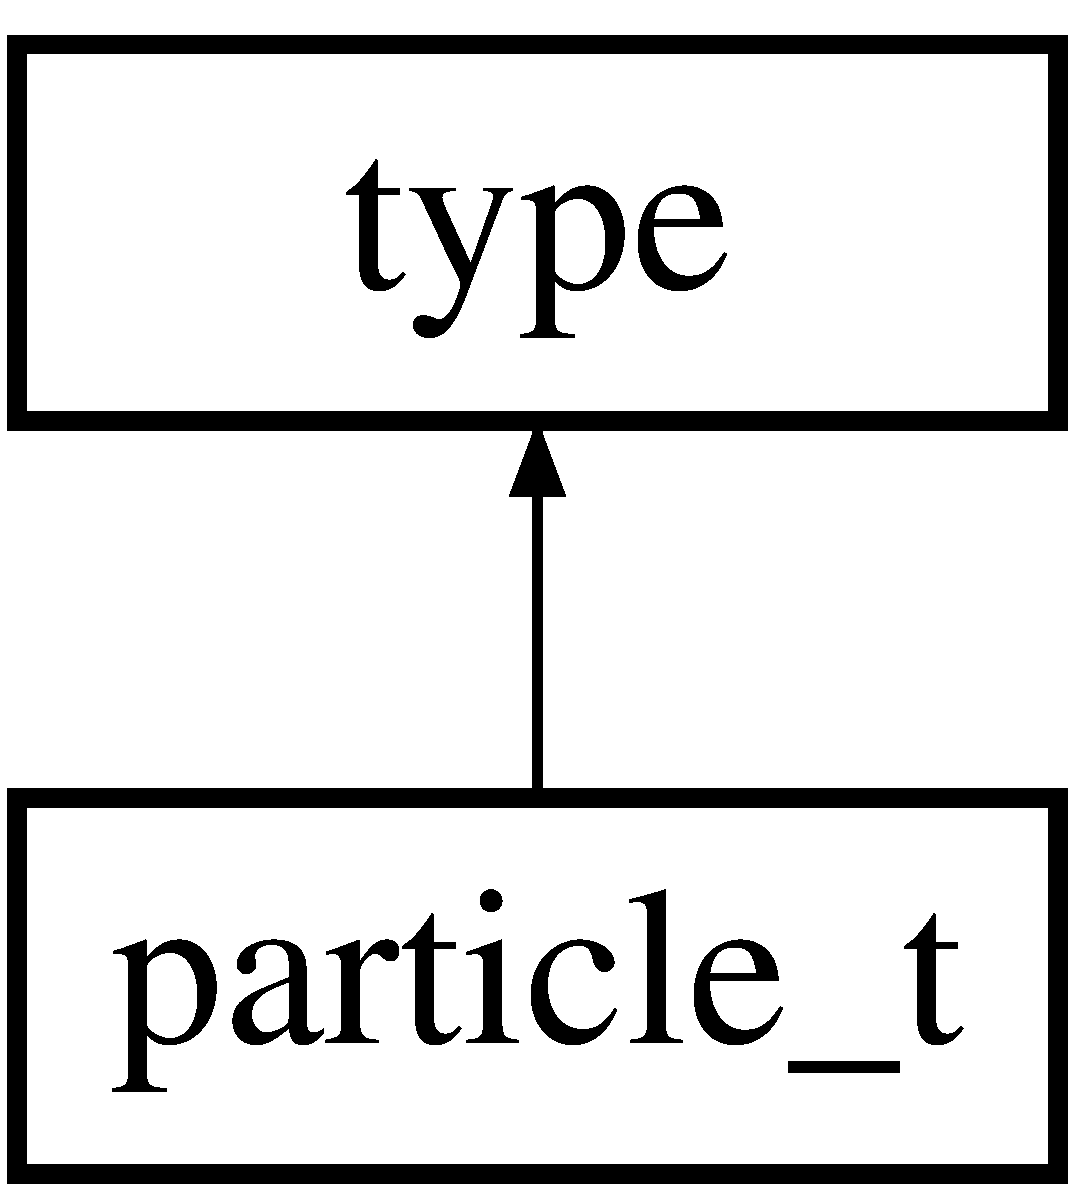
\includegraphics[height=2.000000cm]{classparticle__t}
\end{center}
\end{figure}
\subsection*{Public Types}
\begin{DoxyCompactItemize}
\item 
typedef \-::\hyperlink{namespacexml__schema_acfa24ac68e1a188e7f44c36f7a158bf4}{xml\-\_\-schema\-::int\-\_\-} \hyperlink{classparticle__t_ab30c5ebbd1c4aabb95799f34942b72b2}{par\-Type\-P\-\_\-type}
\item 
typedef \\*
\-::xsd\-::cxx\-::tree\-::traits\\*
$<$ \hyperlink{classparticle__t_ab30c5ebbd1c4aabb95799f34942b72b2}{par\-Type\-P\-\_\-type}, char $>$ \hyperlink{classparticle__t_a8c9ecdb6ceb5ee765e0eb91714ebb8c8}{par\-Type\-P\-\_\-traits}
\item 
typedef \-::\hyperlink{classposition__t}{position\-\_\-t} \hyperlink{classparticle__t_af0130f9c47a13c68332f04389a6f0d2c}{position\-\_\-type}
\item 
typedef \\*
\-::xsd\-::cxx\-::tree\-::traits\\*
$<$ \hyperlink{classparticle__t_af0130f9c47a13c68332f04389a6f0d2c}{position\-\_\-type}, char $>$ \hyperlink{classparticle__t_a3917822f8a2a24b4674e88165aa15d24}{position\-\_\-traits}
\item 
typedef \-::\hyperlink{classvelocity__t}{velocity\-\_\-t} \hyperlink{classparticle__t_a19095006cf2a2dd955fc026420b38512}{velocity\-\_\-type}
\item 
typedef \\*
\-::xsd\-::cxx\-::tree\-::traits\\*
$<$ \hyperlink{classparticle__t_a19095006cf2a2dd955fc026420b38512}{velocity\-\_\-type}, char $>$ \hyperlink{classparticle__t_a97b4645b5dfa77c95f13a142064045db}{velocity\-\_\-traits}
\item 
typedef \-::\hyperlink{namespacexml__schema_a69bfaf24f63a8c18ebd8e21db6b343df}{xml\-\_\-schema\-::decimal} \hyperlink{classparticle__t_a38e9f2cf40d61fa77b19f068d044d294}{mass\-\_\-type}
\item 
typedef \\*
\-::xsd\-::cxx\-::tree\-::traits\\*
$<$ \hyperlink{classparticle__t_a38e9f2cf40d61fa77b19f068d044d294}{mass\-\_\-type}, char,\-::xsd\-::cxx\-::tree\-::schema\-\_\-type\-::decimal $>$ \hyperlink{classparticle__t_ab9c6167e13b441bc375cdc08fa045012}{mass\-\_\-traits}
\end{DoxyCompactItemize}
\subsection*{Public Member Functions}
\begin{DoxyCompactItemize}
\item 
const \hyperlink{classparticle__t_ab30c5ebbd1c4aabb95799f34942b72b2}{par\-Type\-P\-\_\-type} \& \hyperlink{classparticle__t_ac2db0331abd5d49f5eb8b51502dcd05b}{par\-Type\-P} () const 
\item 
\hyperlink{classparticle__t_ab30c5ebbd1c4aabb95799f34942b72b2}{par\-Type\-P\-\_\-type} \& \hyperlink{classparticle__t_ac0dacfd86d82a7905dbd4ebd545d6100}{par\-Type\-P} ()
\item 
void \hyperlink{classparticle__t_afa7c5084c5d3b91017696b601f2d3c13}{par\-Type\-P} (const \hyperlink{classparticle__t_ab30c5ebbd1c4aabb95799f34942b72b2}{par\-Type\-P\-\_\-type} \&x)
\item 
const \hyperlink{classparticle__t_af0130f9c47a13c68332f04389a6f0d2c}{position\-\_\-type} \& \hyperlink{classparticle__t_a3a81b45d11c1756509ca7cf54ca2a3eb}{position} () const 
\item 
\hyperlink{classparticle__t_af0130f9c47a13c68332f04389a6f0d2c}{position\-\_\-type} \& \hyperlink{classparticle__t_ae9b1bbf223bc9fb9f3c48ad71a3b41cf}{position} ()
\item 
void \hyperlink{classparticle__t_acf73b178e4f95313f49c770c55155f9d}{position} (const \hyperlink{classparticle__t_af0130f9c47a13c68332f04389a6f0d2c}{position\-\_\-type} \&x)
\item 
void \hyperlink{classparticle__t_a6749155496ca35433c0fea5d90a4ebf5}{position} (\-::std\-::auto\-\_\-ptr$<$ \hyperlink{classparticle__t_af0130f9c47a13c68332f04389a6f0d2c}{position\-\_\-type} $>$ p)
\item 
const \hyperlink{classparticle__t_a19095006cf2a2dd955fc026420b38512}{velocity\-\_\-type} \& \hyperlink{classparticle__t_a2ebfb7ecdab965984711284cae8d53e9}{velocity} () const 
\item 
\hyperlink{classparticle__t_a19095006cf2a2dd955fc026420b38512}{velocity\-\_\-type} \& \hyperlink{classparticle__t_acf98941eb87e25f1236f86868b9152df}{velocity} ()
\item 
void \hyperlink{classparticle__t_aafc63693d909a979c9eaf360241be925}{velocity} (const \hyperlink{classparticle__t_a19095006cf2a2dd955fc026420b38512}{velocity\-\_\-type} \&x)
\item 
void \hyperlink{classparticle__t_a4ed3bfb4eb196658032b4a3d4ff1bcb1}{velocity} (\-::std\-::auto\-\_\-ptr$<$ \hyperlink{classparticle__t_a19095006cf2a2dd955fc026420b38512}{velocity\-\_\-type} $>$ p)
\item 
const \hyperlink{classparticle__t_a38e9f2cf40d61fa77b19f068d044d294}{mass\-\_\-type} \& \hyperlink{classparticle__t_af8869f0d18a953140a8edf511c314f56}{mass} () const 
\item 
\hyperlink{classparticle__t_a38e9f2cf40d61fa77b19f068d044d294}{mass\-\_\-type} \& \hyperlink{classparticle__t_a86815bfd3b0b1cc4bb133f5f2608becf}{mass} ()
\item 
void \hyperlink{classparticle__t_af1646ca7c088a79e227d62f4a535e3b4}{mass} (const \hyperlink{classparticle__t_a38e9f2cf40d61fa77b19f068d044d294}{mass\-\_\-type} \&x)
\item 
\hyperlink{classparticle__t_aed5c9af92d0ad620cfba62e40c5e9239}{particle\-\_\-t} (const \hyperlink{classparticle__t_ab30c5ebbd1c4aabb95799f34942b72b2}{par\-Type\-P\-\_\-type} \&, const \hyperlink{classparticle__t_af0130f9c47a13c68332f04389a6f0d2c}{position\-\_\-type} \&, const \hyperlink{classparticle__t_a19095006cf2a2dd955fc026420b38512}{velocity\-\_\-type} \&, const \hyperlink{classparticle__t_a38e9f2cf40d61fa77b19f068d044d294}{mass\-\_\-type} \&)
\item 
\hyperlink{classparticle__t_a07a9ce2f3386bfe065bb3af0680c1b0f}{particle\-\_\-t} (const \hyperlink{classparticle__t_ab30c5ebbd1c4aabb95799f34942b72b2}{par\-Type\-P\-\_\-type} \&,\-::std\-::auto\-\_\-ptr$<$ \hyperlink{classparticle__t_af0130f9c47a13c68332f04389a6f0d2c}{position\-\_\-type} $>$ \&,\-::std\-::auto\-\_\-ptr$<$ \hyperlink{classparticle__t_a19095006cf2a2dd955fc026420b38512}{velocity\-\_\-type} $>$ \&, const \hyperlink{classparticle__t_a38e9f2cf40d61fa77b19f068d044d294}{mass\-\_\-type} \&)
\item 
\hyperlink{classparticle__t_a7ee9d95821b0e1840f4834029fb04c3b}{particle\-\_\-t} (const \-::xercesc\-::\-D\-O\-M\-Element \&e,\-::\hyperlink{namespacexml__schema_a0612287d030cb2732d31a45b258fdc87}{xml\-\_\-schema\-::flags} f=0,\-::\hyperlink{namespacexml__schema_ada9aa30dc722e93ee2ed7243085402a5}{xml\-\_\-schema\-::container} $\ast$c=0)
\item 
\hyperlink{classparticle__t_a393bb37e0c1e50ee3e2c2d1b7aef0f1a}{particle\-\_\-t} (const \hyperlink{classparticle__t}{particle\-\_\-t} \&x,\-::\hyperlink{namespacexml__schema_a0612287d030cb2732d31a45b258fdc87}{xml\-\_\-schema\-::flags} f=0,\-::\hyperlink{namespacexml__schema_ada9aa30dc722e93ee2ed7243085402a5}{xml\-\_\-schema\-::container} $\ast$c=0)
\item 
virtual \hyperlink{classparticle__t}{particle\-\_\-t} $\ast$ \hyperlink{classparticle__t_a7f3173200bb6bc6370c5b3284b5b97eb}{\-\_\-clone} (\-::\hyperlink{namespacexml__schema_a0612287d030cb2732d31a45b258fdc87}{xml\-\_\-schema\-::flags} f=0,\-::\hyperlink{namespacexml__schema_ada9aa30dc722e93ee2ed7243085402a5}{xml\-\_\-schema\-::container} $\ast$c=0) const 
\item 
virtual \hyperlink{classparticle__t_aadfae8ce4510f63d48a4dc207f890d92}{$\sim$particle\-\_\-t} ()
\end{DoxyCompactItemize}
\subsection*{Protected Member Functions}
\begin{DoxyCompactItemize}
\item 
void \hyperlink{classparticle__t_acb15084033be62d2b49f72496e569497}{parse} (\-::xsd\-::cxx\-::xml\-::dom\-::parser$<$ char $>$ \&,\-::\hyperlink{namespacexml__schema_a0612287d030cb2732d31a45b258fdc87}{xml\-\_\-schema\-::flags})
\end{DoxyCompactItemize}
\subsection*{Protected Attributes}
\begin{DoxyCompactItemize}
\item 
\-::xsd\-::cxx\-::tree\-::one\\*
$<$ \hyperlink{classparticle__t_ab30c5ebbd1c4aabb95799f34942b72b2}{par\-Type\-P\-\_\-type} $>$ \hyperlink{classparticle__t_a766d1a1cbb2d1deb3895f4c86ee5b6d2}{par\-Type\-P\-\_\-}
\item 
\-::xsd\-::cxx\-::tree\-::one\\*
$<$ \hyperlink{classparticle__t_af0130f9c47a13c68332f04389a6f0d2c}{position\-\_\-type} $>$ \hyperlink{classparticle__t_a9617dc13afdc37ecd76d16f2abf14b60}{position\-\_\-}
\item 
\-::xsd\-::cxx\-::tree\-::one\\*
$<$ \hyperlink{classparticle__t_a19095006cf2a2dd955fc026420b38512}{velocity\-\_\-type} $>$ \hyperlink{classparticle__t_a4e8569ca9f6438eca58864d57ce73b39}{velocity\-\_\-}
\item 
\-::xsd\-::cxx\-::tree\-::one$<$ \hyperlink{classparticle__t_a38e9f2cf40d61fa77b19f068d044d294}{mass\-\_\-type} $>$ \hyperlink{classparticle__t_a5c33cbf5a5ac4b4d6ef74cfc19366f77}{mass\-\_\-}
\end{DoxyCompactItemize}


\subsection{Member Typedef Documentation}
\hypertarget{classparticle__t_ab9c6167e13b441bc375cdc08fa045012}{\index{particle\-\_\-t@{particle\-\_\-t}!mass\-\_\-traits@{mass\-\_\-traits}}
\index{mass\-\_\-traits@{mass\-\_\-traits}!particle_t@{particle\-\_\-t}}
\subsubsection[{mass\-\_\-traits}]{\setlength{\rightskip}{0pt plus 5cm}typedef \-::xsd\-::cxx\-::tree\-::traits$<$ {\bf mass\-\_\-type}, char, \-::xsd\-::cxx\-::tree\-::schema\-\_\-type\-::decimal $>$ {\bf particle\-\_\-t\-::mass\-\_\-traits}}}\label{classparticle__t_ab9c6167e13b441bc375cdc08fa045012}
\hypertarget{classparticle__t_a38e9f2cf40d61fa77b19f068d044d294}{\index{particle\-\_\-t@{particle\-\_\-t}!mass\-\_\-type@{mass\-\_\-type}}
\index{mass\-\_\-type@{mass\-\_\-type}!particle_t@{particle\-\_\-t}}
\subsubsection[{mass\-\_\-type}]{\setlength{\rightskip}{0pt plus 5cm}typedef \-::{\bf xml\-\_\-schema\-::decimal} {\bf particle\-\_\-t\-::mass\-\_\-type}}}\label{classparticle__t_a38e9f2cf40d61fa77b19f068d044d294}
\hypertarget{classparticle__t_a8c9ecdb6ceb5ee765e0eb91714ebb8c8}{\index{particle\-\_\-t@{particle\-\_\-t}!par\-Type\-P\-\_\-traits@{par\-Type\-P\-\_\-traits}}
\index{par\-Type\-P\-\_\-traits@{par\-Type\-P\-\_\-traits}!particle_t@{particle\-\_\-t}}
\subsubsection[{par\-Type\-P\-\_\-traits}]{\setlength{\rightskip}{0pt plus 5cm}typedef \-::xsd\-::cxx\-::tree\-::traits$<$ {\bf par\-Type\-P\-\_\-type}, char $>$ {\bf particle\-\_\-t\-::par\-Type\-P\-\_\-traits}}}\label{classparticle__t_a8c9ecdb6ceb5ee765e0eb91714ebb8c8}
\hypertarget{classparticle__t_ab30c5ebbd1c4aabb95799f34942b72b2}{\index{particle\-\_\-t@{particle\-\_\-t}!par\-Type\-P\-\_\-type@{par\-Type\-P\-\_\-type}}
\index{par\-Type\-P\-\_\-type@{par\-Type\-P\-\_\-type}!particle_t@{particle\-\_\-t}}
\subsubsection[{par\-Type\-P\-\_\-type}]{\setlength{\rightskip}{0pt plus 5cm}typedef \-::{\bf xml\-\_\-schema\-::int\-\_\-} {\bf particle\-\_\-t\-::par\-Type\-P\-\_\-type}}}\label{classparticle__t_ab30c5ebbd1c4aabb95799f34942b72b2}
\hypertarget{classparticle__t_a3917822f8a2a24b4674e88165aa15d24}{\index{particle\-\_\-t@{particle\-\_\-t}!position\-\_\-traits@{position\-\_\-traits}}
\index{position\-\_\-traits@{position\-\_\-traits}!particle_t@{particle\-\_\-t}}
\subsubsection[{position\-\_\-traits}]{\setlength{\rightskip}{0pt plus 5cm}typedef \-::xsd\-::cxx\-::tree\-::traits$<$ {\bf position\-\_\-type}, char $>$ {\bf particle\-\_\-t\-::position\-\_\-traits}}}\label{classparticle__t_a3917822f8a2a24b4674e88165aa15d24}
\hypertarget{classparticle__t_af0130f9c47a13c68332f04389a6f0d2c}{\index{particle\-\_\-t@{particle\-\_\-t}!position\-\_\-type@{position\-\_\-type}}
\index{position\-\_\-type@{position\-\_\-type}!particle_t@{particle\-\_\-t}}
\subsubsection[{position\-\_\-type}]{\setlength{\rightskip}{0pt plus 5cm}typedef \-::{\bf position\-\_\-t} {\bf particle\-\_\-t\-::position\-\_\-type}}}\label{classparticle__t_af0130f9c47a13c68332f04389a6f0d2c}
\hypertarget{classparticle__t_a97b4645b5dfa77c95f13a142064045db}{\index{particle\-\_\-t@{particle\-\_\-t}!velocity\-\_\-traits@{velocity\-\_\-traits}}
\index{velocity\-\_\-traits@{velocity\-\_\-traits}!particle_t@{particle\-\_\-t}}
\subsubsection[{velocity\-\_\-traits}]{\setlength{\rightskip}{0pt plus 5cm}typedef \-::xsd\-::cxx\-::tree\-::traits$<$ {\bf velocity\-\_\-type}, char $>$ {\bf particle\-\_\-t\-::velocity\-\_\-traits}}}\label{classparticle__t_a97b4645b5dfa77c95f13a142064045db}
\hypertarget{classparticle__t_a19095006cf2a2dd955fc026420b38512}{\index{particle\-\_\-t@{particle\-\_\-t}!velocity\-\_\-type@{velocity\-\_\-type}}
\index{velocity\-\_\-type@{velocity\-\_\-type}!particle_t@{particle\-\_\-t}}
\subsubsection[{velocity\-\_\-type}]{\setlength{\rightskip}{0pt plus 5cm}typedef \-::{\bf velocity\-\_\-t} {\bf particle\-\_\-t\-::velocity\-\_\-type}}}\label{classparticle__t_a19095006cf2a2dd955fc026420b38512}


\subsection{Constructor \& Destructor Documentation}
\hypertarget{classparticle__t_aed5c9af92d0ad620cfba62e40c5e9239}{\index{particle\-\_\-t@{particle\-\_\-t}!particle\-\_\-t@{particle\-\_\-t}}
\index{particle\-\_\-t@{particle\-\_\-t}!particle_t@{particle\-\_\-t}}
\subsubsection[{particle\-\_\-t}]{\setlength{\rightskip}{0pt plus 5cm}particle\-\_\-t\-::particle\-\_\-t (
\begin{DoxyParamCaption}
\item[{const {\bf par\-Type\-P\-\_\-type} \&}]{par\-Type\-P, }
\item[{const {\bf position\-\_\-type} \&}]{position, }
\item[{const {\bf velocity\-\_\-type} \&}]{velocity, }
\item[{const {\bf mass\-\_\-type} \&}]{mass}
\end{DoxyParamCaption}
)}}\label{classparticle__t_aed5c9af92d0ad620cfba62e40c5e9239}
\hypertarget{classparticle__t_a07a9ce2f3386bfe065bb3af0680c1b0f}{\index{particle\-\_\-t@{particle\-\_\-t}!particle\-\_\-t@{particle\-\_\-t}}
\index{particle\-\_\-t@{particle\-\_\-t}!particle_t@{particle\-\_\-t}}
\subsubsection[{particle\-\_\-t}]{\setlength{\rightskip}{0pt plus 5cm}particle\-\_\-t\-::particle\-\_\-t (
\begin{DoxyParamCaption}
\item[{const {\bf par\-Type\-P\-\_\-type} \&}]{par\-Type\-P, }
\item[{\-::std\-::auto\-\_\-ptr$<$ {\bf position\-\_\-type} $>$ \&}]{position, }
\item[{\-::std\-::auto\-\_\-ptr$<$ {\bf velocity\-\_\-type} $>$ \&}]{velocity, }
\item[{const {\bf mass\-\_\-type} \&}]{mass}
\end{DoxyParamCaption}
)}}\label{classparticle__t_a07a9ce2f3386bfe065bb3af0680c1b0f}
\hypertarget{classparticle__t_a7ee9d95821b0e1840f4834029fb04c3b}{\index{particle\-\_\-t@{particle\-\_\-t}!particle\-\_\-t@{particle\-\_\-t}}
\index{particle\-\_\-t@{particle\-\_\-t}!particle_t@{particle\-\_\-t}}
\subsubsection[{particle\-\_\-t}]{\setlength{\rightskip}{0pt plus 5cm}particle\-\_\-t\-::particle\-\_\-t (
\begin{DoxyParamCaption}
\item[{const \-::xercesc\-::\-D\-O\-M\-Element \&}]{e, }
\item[{\-::{\bf xml\-\_\-schema\-::flags}}]{f = {\ttfamily 0}, }
\item[{\-::{\bf xml\-\_\-schema\-::container} $\ast$}]{c = {\ttfamily 0}}
\end{DoxyParamCaption}
)}}\label{classparticle__t_a7ee9d95821b0e1840f4834029fb04c3b}
\hypertarget{classparticle__t_a393bb37e0c1e50ee3e2c2d1b7aef0f1a}{\index{particle\-\_\-t@{particle\-\_\-t}!particle\-\_\-t@{particle\-\_\-t}}
\index{particle\-\_\-t@{particle\-\_\-t}!particle_t@{particle\-\_\-t}}
\subsubsection[{particle\-\_\-t}]{\setlength{\rightskip}{0pt plus 5cm}particle\-\_\-t\-::particle\-\_\-t (
\begin{DoxyParamCaption}
\item[{const {\bf particle\-\_\-t} \&}]{x, }
\item[{\-::{\bf xml\-\_\-schema\-::flags}}]{f = {\ttfamily 0}, }
\item[{\-::{\bf xml\-\_\-schema\-::container} $\ast$}]{c = {\ttfamily 0}}
\end{DoxyParamCaption}
)}}\label{classparticle__t_a393bb37e0c1e50ee3e2c2d1b7aef0f1a}
\hypertarget{classparticle__t_aadfae8ce4510f63d48a4dc207f890d92}{\index{particle\-\_\-t@{particle\-\_\-t}!$\sim$particle\-\_\-t@{$\sim$particle\-\_\-t}}
\index{$\sim$particle\-\_\-t@{$\sim$particle\-\_\-t}!particle_t@{particle\-\_\-t}}
\subsubsection[{$\sim$particle\-\_\-t}]{\setlength{\rightskip}{0pt plus 5cm}particle\-\_\-t\-::$\sim$particle\-\_\-t (
\begin{DoxyParamCaption}
{}
\end{DoxyParamCaption}
)\hspace{0.3cm}{\ttfamily [virtual]}}}\label{classparticle__t_aadfae8ce4510f63d48a4dc207f890d92}


\subsection{Member Function Documentation}
\hypertarget{classparticle__t_a7f3173200bb6bc6370c5b3284b5b97eb}{\index{particle\-\_\-t@{particle\-\_\-t}!\-\_\-clone@{\-\_\-clone}}
\index{\-\_\-clone@{\-\_\-clone}!particle_t@{particle\-\_\-t}}
\subsubsection[{\-\_\-clone}]{\setlength{\rightskip}{0pt plus 5cm}{\bf particle\-\_\-t} $\ast$ particle\-\_\-t\-::\-\_\-clone (
\begin{DoxyParamCaption}
\item[{\-::{\bf xml\-\_\-schema\-::flags}}]{f = {\ttfamily 0}, }
\item[{\-::{\bf xml\-\_\-schema\-::container} $\ast$}]{c = {\ttfamily 0}}
\end{DoxyParamCaption}
) const\hspace{0.3cm}{\ttfamily [virtual]}}}\label{classparticle__t_a7f3173200bb6bc6370c5b3284b5b97eb}
\hypertarget{classparticle__t_af8869f0d18a953140a8edf511c314f56}{\index{particle\-\_\-t@{particle\-\_\-t}!mass@{mass}}
\index{mass@{mass}!particle_t@{particle\-\_\-t}}
\subsubsection[{mass}]{\setlength{\rightskip}{0pt plus 5cm}const {\bf particle\-\_\-t\-::mass\-\_\-type} \& particle\-\_\-t\-::mass (
\begin{DoxyParamCaption}
{}
\end{DoxyParamCaption}
) const}}\label{classparticle__t_af8869f0d18a953140a8edf511c314f56}
\hypertarget{classparticle__t_a86815bfd3b0b1cc4bb133f5f2608becf}{\index{particle\-\_\-t@{particle\-\_\-t}!mass@{mass}}
\index{mass@{mass}!particle_t@{particle\-\_\-t}}
\subsubsection[{mass}]{\setlength{\rightskip}{0pt plus 5cm}{\bf particle\-\_\-t\-::mass\-\_\-type} \& particle\-\_\-t\-::mass (
\begin{DoxyParamCaption}
{}
\end{DoxyParamCaption}
)}}\label{classparticle__t_a86815bfd3b0b1cc4bb133f5f2608becf}
\hypertarget{classparticle__t_af1646ca7c088a79e227d62f4a535e3b4}{\index{particle\-\_\-t@{particle\-\_\-t}!mass@{mass}}
\index{mass@{mass}!particle_t@{particle\-\_\-t}}
\subsubsection[{mass}]{\setlength{\rightskip}{0pt plus 5cm}void particle\-\_\-t\-::mass (
\begin{DoxyParamCaption}
\item[{const {\bf mass\-\_\-type} \&}]{x}
\end{DoxyParamCaption}
)}}\label{classparticle__t_af1646ca7c088a79e227d62f4a535e3b4}
\hypertarget{classparticle__t_acb15084033be62d2b49f72496e569497}{\index{particle\-\_\-t@{particle\-\_\-t}!parse@{parse}}
\index{parse@{parse}!particle_t@{particle\-\_\-t}}
\subsubsection[{parse}]{\setlength{\rightskip}{0pt plus 5cm}void particle\-\_\-t\-::parse (
\begin{DoxyParamCaption}
\item[{\-::xsd\-::cxx\-::xml\-::dom\-::parser$<$ char $>$ \&}]{p, }
\item[{\-::{\bf xml\-\_\-schema\-::flags}}]{f}
\end{DoxyParamCaption}
)\hspace{0.3cm}{\ttfamily [protected]}}}\label{classparticle__t_acb15084033be62d2b49f72496e569497}
\hypertarget{classparticle__t_ac2db0331abd5d49f5eb8b51502dcd05b}{\index{particle\-\_\-t@{particle\-\_\-t}!par\-Type\-P@{par\-Type\-P}}
\index{par\-Type\-P@{par\-Type\-P}!particle_t@{particle\-\_\-t}}
\subsubsection[{par\-Type\-P}]{\setlength{\rightskip}{0pt plus 5cm}const {\bf particle\-\_\-t\-::par\-Type\-P\-\_\-type} \& particle\-\_\-t\-::par\-Type\-P (
\begin{DoxyParamCaption}
{}
\end{DoxyParamCaption}
) const}}\label{classparticle__t_ac2db0331abd5d49f5eb8b51502dcd05b}
\hypertarget{classparticle__t_ac0dacfd86d82a7905dbd4ebd545d6100}{\index{particle\-\_\-t@{particle\-\_\-t}!par\-Type\-P@{par\-Type\-P}}
\index{par\-Type\-P@{par\-Type\-P}!particle_t@{particle\-\_\-t}}
\subsubsection[{par\-Type\-P}]{\setlength{\rightskip}{0pt plus 5cm}{\bf particle\-\_\-t\-::par\-Type\-P\-\_\-type} \& particle\-\_\-t\-::par\-Type\-P (
\begin{DoxyParamCaption}
{}
\end{DoxyParamCaption}
)}}\label{classparticle__t_ac0dacfd86d82a7905dbd4ebd545d6100}
\hypertarget{classparticle__t_afa7c5084c5d3b91017696b601f2d3c13}{\index{particle\-\_\-t@{particle\-\_\-t}!par\-Type\-P@{par\-Type\-P}}
\index{par\-Type\-P@{par\-Type\-P}!particle_t@{particle\-\_\-t}}
\subsubsection[{par\-Type\-P}]{\setlength{\rightskip}{0pt plus 5cm}void particle\-\_\-t\-::par\-Type\-P (
\begin{DoxyParamCaption}
\item[{const {\bf par\-Type\-P\-\_\-type} \&}]{x}
\end{DoxyParamCaption}
)}}\label{classparticle__t_afa7c5084c5d3b91017696b601f2d3c13}
\hypertarget{classparticle__t_a3a81b45d11c1756509ca7cf54ca2a3eb}{\index{particle\-\_\-t@{particle\-\_\-t}!position@{position}}
\index{position@{position}!particle_t@{particle\-\_\-t}}
\subsubsection[{position}]{\setlength{\rightskip}{0pt plus 5cm}const {\bf particle\-\_\-t\-::position\-\_\-type} \& particle\-\_\-t\-::position (
\begin{DoxyParamCaption}
{}
\end{DoxyParamCaption}
) const}}\label{classparticle__t_a3a81b45d11c1756509ca7cf54ca2a3eb}
\hypertarget{classparticle__t_ae9b1bbf223bc9fb9f3c48ad71a3b41cf}{\index{particle\-\_\-t@{particle\-\_\-t}!position@{position}}
\index{position@{position}!particle_t@{particle\-\_\-t}}
\subsubsection[{position}]{\setlength{\rightskip}{0pt plus 5cm}{\bf particle\-\_\-t\-::position\-\_\-type} \& particle\-\_\-t\-::position (
\begin{DoxyParamCaption}
{}
\end{DoxyParamCaption}
)}}\label{classparticle__t_ae9b1bbf223bc9fb9f3c48ad71a3b41cf}
\hypertarget{classparticle__t_acf73b178e4f95313f49c770c55155f9d}{\index{particle\-\_\-t@{particle\-\_\-t}!position@{position}}
\index{position@{position}!particle_t@{particle\-\_\-t}}
\subsubsection[{position}]{\setlength{\rightskip}{0pt plus 5cm}void particle\-\_\-t\-::position (
\begin{DoxyParamCaption}
\item[{const {\bf position\-\_\-type} \&}]{x}
\end{DoxyParamCaption}
)}}\label{classparticle__t_acf73b178e4f95313f49c770c55155f9d}
\hypertarget{classparticle__t_a6749155496ca35433c0fea5d90a4ebf5}{\index{particle\-\_\-t@{particle\-\_\-t}!position@{position}}
\index{position@{position}!particle_t@{particle\-\_\-t}}
\subsubsection[{position}]{\setlength{\rightskip}{0pt plus 5cm}void particle\-\_\-t\-::position (
\begin{DoxyParamCaption}
\item[{\-::std\-::auto\-\_\-ptr$<$ {\bf position\-\_\-type} $>$}]{p}
\end{DoxyParamCaption}
)}}\label{classparticle__t_a6749155496ca35433c0fea5d90a4ebf5}
\hypertarget{classparticle__t_a2ebfb7ecdab965984711284cae8d53e9}{\index{particle\-\_\-t@{particle\-\_\-t}!velocity@{velocity}}
\index{velocity@{velocity}!particle_t@{particle\-\_\-t}}
\subsubsection[{velocity}]{\setlength{\rightskip}{0pt plus 5cm}const {\bf particle\-\_\-t\-::velocity\-\_\-type} \& particle\-\_\-t\-::velocity (
\begin{DoxyParamCaption}
{}
\end{DoxyParamCaption}
) const}}\label{classparticle__t_a2ebfb7ecdab965984711284cae8d53e9}
\hypertarget{classparticle__t_acf98941eb87e25f1236f86868b9152df}{\index{particle\-\_\-t@{particle\-\_\-t}!velocity@{velocity}}
\index{velocity@{velocity}!particle_t@{particle\-\_\-t}}
\subsubsection[{velocity}]{\setlength{\rightskip}{0pt plus 5cm}{\bf particle\-\_\-t\-::velocity\-\_\-type} \& particle\-\_\-t\-::velocity (
\begin{DoxyParamCaption}
{}
\end{DoxyParamCaption}
)}}\label{classparticle__t_acf98941eb87e25f1236f86868b9152df}
\hypertarget{classparticle__t_aafc63693d909a979c9eaf360241be925}{\index{particle\-\_\-t@{particle\-\_\-t}!velocity@{velocity}}
\index{velocity@{velocity}!particle_t@{particle\-\_\-t}}
\subsubsection[{velocity}]{\setlength{\rightskip}{0pt plus 5cm}void particle\-\_\-t\-::velocity (
\begin{DoxyParamCaption}
\item[{const {\bf velocity\-\_\-type} \&}]{x}
\end{DoxyParamCaption}
)}}\label{classparticle__t_aafc63693d909a979c9eaf360241be925}
\hypertarget{classparticle__t_a4ed3bfb4eb196658032b4a3d4ff1bcb1}{\index{particle\-\_\-t@{particle\-\_\-t}!velocity@{velocity}}
\index{velocity@{velocity}!particle_t@{particle\-\_\-t}}
\subsubsection[{velocity}]{\setlength{\rightskip}{0pt plus 5cm}void particle\-\_\-t\-::velocity (
\begin{DoxyParamCaption}
\item[{\-::std\-::auto\-\_\-ptr$<$ {\bf velocity\-\_\-type} $>$}]{p}
\end{DoxyParamCaption}
)}}\label{classparticle__t_a4ed3bfb4eb196658032b4a3d4ff1bcb1}


\subsection{Member Data Documentation}
\hypertarget{classparticle__t_a5c33cbf5a5ac4b4d6ef74cfc19366f77}{\index{particle\-\_\-t@{particle\-\_\-t}!mass\-\_\-@{mass\-\_\-}}
\index{mass\-\_\-@{mass\-\_\-}!particle_t@{particle\-\_\-t}}
\subsubsection[{mass\-\_\-}]{\setlength{\rightskip}{0pt plus 5cm}\-::xsd\-::cxx\-::tree\-::one$<$ {\bf mass\-\_\-type} $>$ particle\-\_\-t\-::mass\-\_\-\hspace{0.3cm}{\ttfamily [protected]}}}\label{classparticle__t_a5c33cbf5a5ac4b4d6ef74cfc19366f77}
\hypertarget{classparticle__t_a766d1a1cbb2d1deb3895f4c86ee5b6d2}{\index{particle\-\_\-t@{particle\-\_\-t}!par\-Type\-P\-\_\-@{par\-Type\-P\-\_\-}}
\index{par\-Type\-P\-\_\-@{par\-Type\-P\-\_\-}!particle_t@{particle\-\_\-t}}
\subsubsection[{par\-Type\-P\-\_\-}]{\setlength{\rightskip}{0pt plus 5cm}\-::xsd\-::cxx\-::tree\-::one$<$ {\bf par\-Type\-P\-\_\-type} $>$ particle\-\_\-t\-::par\-Type\-P\-\_\-\hspace{0.3cm}{\ttfamily [protected]}}}\label{classparticle__t_a766d1a1cbb2d1deb3895f4c86ee5b6d2}
\hypertarget{classparticle__t_a9617dc13afdc37ecd76d16f2abf14b60}{\index{particle\-\_\-t@{particle\-\_\-t}!position\-\_\-@{position\-\_\-}}
\index{position\-\_\-@{position\-\_\-}!particle_t@{particle\-\_\-t}}
\subsubsection[{position\-\_\-}]{\setlength{\rightskip}{0pt plus 5cm}\-::xsd\-::cxx\-::tree\-::one$<$ {\bf position\-\_\-type} $>$ particle\-\_\-t\-::position\-\_\-\hspace{0.3cm}{\ttfamily [protected]}}}\label{classparticle__t_a9617dc13afdc37ecd76d16f2abf14b60}
\hypertarget{classparticle__t_a4e8569ca9f6438eca58864d57ce73b39}{\index{particle\-\_\-t@{particle\-\_\-t}!velocity\-\_\-@{velocity\-\_\-}}
\index{velocity\-\_\-@{velocity\-\_\-}!particle_t@{particle\-\_\-t}}
\subsubsection[{velocity\-\_\-}]{\setlength{\rightskip}{0pt plus 5cm}\-::xsd\-::cxx\-::tree\-::one$<$ {\bf velocity\-\_\-type} $>$ particle\-\_\-t\-::velocity\-\_\-\hspace{0.3cm}{\ttfamily [protected]}}}\label{classparticle__t_a4e8569ca9f6438eca58864d57ce73b39}


The documentation for this class was generated from the following files\-:\begin{DoxyCompactItemize}
\item 
src/utils/\hyperlink{InputParticles_8h}{Input\-Particles.\-h}\item 
src/utils/\hyperlink{InputParticles_8cpp}{Input\-Particles.\-cpp}\end{DoxyCompactItemize}

\hypertarget{classutils_1_1ParticleContainer}{\section{utils\-:\-:Particle\-Container Class Reference}
\label{classutils_1_1ParticleContainer}\index{utils\-::\-Particle\-Container@{utils\-::\-Particle\-Container}}
}


{\ttfamily \#include $<$Particle\-Container.\-h$>$}

\subsection*{Public Member Functions}
\begin{DoxyCompactItemize}
\item 
\hyperlink{classutils_1_1ParticleContainer_a76d21bdb5141158cf664d65e2d8b1db7}{Particle\-Container} ()
\item 
\hyperlink{classutils_1_1ParticleContainer_a9629a8d31a3aa8c2fe944307c1263b66}{$\sim$\-Particle\-Container} ()
\item 
void \hyperlink{classutils_1_1ParticleContainer_abc060d13bb939123fd0bf1631e0562ca}{initialize} (std\-::list$<$ \hyperlink{classParticle}{Particle} $>$ \&particles\-\_\-arg)
\item 
\hyperlink{classutils_1_1ParticleIterator}{utils\-::\-Particle\-Iterator} \hyperlink{classutils_1_1ParticleContainer_a54e64306f644d9c1d7ac47694592023f}{begin} ()
\item 
\hyperlink{classutils_1_1ParticleIterator}{utils\-::\-Particle\-Iterator} \hyperlink{classutils_1_1ParticleContainer_a9e1b338ace1db41a8f95c69e1bb0817d}{end} ()
\item 
std\-::list$<$ \hyperlink{classParticle}{Particle} $>$ \& \hyperlink{classutils_1_1ParticleContainer_ad3ab05ad52512893f4f251f3219bc11d}{get\-List} ()
\item 
int \hyperlink{classutils_1_1ParticleContainer_ae67310a062690e380c78625b1f944537}{size} ()
\end{DoxyCompactItemize}
\subsection*{Private Attributes}
\begin{DoxyCompactItemize}
\item 
std\-::list$<$ \hyperlink{classParticle}{Particle} $>$ \hyperlink{classutils_1_1ParticleContainer_a112ab237df50a570431ecce15d151e45}{particles}
\end{DoxyCompactItemize}


\subsection{Constructor \& Destructor Documentation}
\hypertarget{classutils_1_1ParticleContainer_a76d21bdb5141158cf664d65e2d8b1db7}{\index{utils\-::\-Particle\-Container@{utils\-::\-Particle\-Container}!Particle\-Container@{Particle\-Container}}
\index{Particle\-Container@{Particle\-Container}!utils::ParticleContainer@{utils\-::\-Particle\-Container}}
\subsubsection[{Particle\-Container}]{\setlength{\rightskip}{0pt plus 5cm}Particle\-Container\-::\-Particle\-Container (
\begin{DoxyParamCaption}
{}
\end{DoxyParamCaption}
)}}\label{classutils_1_1ParticleContainer_a76d21bdb5141158cf664d65e2d8b1db7}
\hypertarget{classutils_1_1ParticleContainer_a9629a8d31a3aa8c2fe944307c1263b66}{\index{utils\-::\-Particle\-Container@{utils\-::\-Particle\-Container}!$\sim$\-Particle\-Container@{$\sim$\-Particle\-Container}}
\index{$\sim$\-Particle\-Container@{$\sim$\-Particle\-Container}!utils::ParticleContainer@{utils\-::\-Particle\-Container}}
\subsubsection[{$\sim$\-Particle\-Container}]{\setlength{\rightskip}{0pt plus 5cm}Particle\-Container\-::$\sim$\-Particle\-Container (
\begin{DoxyParamCaption}
{}
\end{DoxyParamCaption}
)}}\label{classutils_1_1ParticleContainer_a9629a8d31a3aa8c2fe944307c1263b66}


\subsection{Member Function Documentation}
\hypertarget{classutils_1_1ParticleContainer_a54e64306f644d9c1d7ac47694592023f}{\index{utils\-::\-Particle\-Container@{utils\-::\-Particle\-Container}!begin@{begin}}
\index{begin@{begin}!utils::ParticleContainer@{utils\-::\-Particle\-Container}}
\subsubsection[{begin}]{\setlength{\rightskip}{0pt plus 5cm}{\bf Particle\-Iterator} Particle\-Container\-::begin (
\begin{DoxyParamCaption}
{}
\end{DoxyParamCaption}
)}}\label{classutils_1_1ParticleContainer_a54e64306f644d9c1d7ac47694592023f}
\begin{DoxyReturn}{Returns}
the first element of the container 
\end{DoxyReturn}
\hypertarget{classutils_1_1ParticleContainer_a9e1b338ace1db41a8f95c69e1bb0817d}{\index{utils\-::\-Particle\-Container@{utils\-::\-Particle\-Container}!end@{end}}
\index{end@{end}!utils::ParticleContainer@{utils\-::\-Particle\-Container}}
\subsubsection[{end}]{\setlength{\rightskip}{0pt plus 5cm}{\bf Particle\-Iterator} Particle\-Container\-::end (
\begin{DoxyParamCaption}
{}
\end{DoxyParamCaption}
)}}\label{classutils_1_1ParticleContainer_a9e1b338ace1db41a8f95c69e1bb0817d}
\begin{DoxyReturn}{Returns}
the last element of the container 
\end{DoxyReturn}
\hypertarget{classutils_1_1ParticleContainer_ad3ab05ad52512893f4f251f3219bc11d}{\index{utils\-::\-Particle\-Container@{utils\-::\-Particle\-Container}!get\-List@{get\-List}}
\index{get\-List@{get\-List}!utils::ParticleContainer@{utils\-::\-Particle\-Container}}
\subsubsection[{get\-List}]{\setlength{\rightskip}{0pt plus 5cm}std\-::list$<$ {\bf Particle} $>$ \& Particle\-Container\-::get\-List (
\begin{DoxyParamCaption}
{}
\end{DoxyParamCaption}
)}}\label{classutils_1_1ParticleContainer_ad3ab05ad52512893f4f251f3219bc11d}
@ return the particles list \hypertarget{classutils_1_1ParticleContainer_abc060d13bb939123fd0bf1631e0562ca}{\index{utils\-::\-Particle\-Container@{utils\-::\-Particle\-Container}!initialize@{initialize}}
\index{initialize@{initialize}!utils::ParticleContainer@{utils\-::\-Particle\-Container}}
\subsubsection[{initialize}]{\setlength{\rightskip}{0pt plus 5cm}void Particle\-Container\-::initialize (
\begin{DoxyParamCaption}
\item[{std\-::list$<$ {\bf Particle} $>$ \&}]{particles\-\_\-arg}
\end{DoxyParamCaption}
)}}\label{classutils_1_1ParticleContainer_abc060d13bb939123fd0bf1631e0562ca}
fills the particles list 
\begin{DoxyParams}{Parameters}
{\em the} & list \\
\hline
\end{DoxyParams}
\hypertarget{classutils_1_1ParticleContainer_ae67310a062690e380c78625b1f944537}{\index{utils\-::\-Particle\-Container@{utils\-::\-Particle\-Container}!size@{size}}
\index{size@{size}!utils::ParticleContainer@{utils\-::\-Particle\-Container}}
\subsubsection[{size}]{\setlength{\rightskip}{0pt plus 5cm}int Particle\-Container\-::size (
\begin{DoxyParamCaption}
{}
\end{DoxyParamCaption}
)}}\label{classutils_1_1ParticleContainer_ae67310a062690e380c78625b1f944537}
@ return the size of the size 

\subsection{Member Data Documentation}
\hypertarget{classutils_1_1ParticleContainer_a112ab237df50a570431ecce15d151e45}{\index{utils\-::\-Particle\-Container@{utils\-::\-Particle\-Container}!particles@{particles}}
\index{particles@{particles}!utils::ParticleContainer@{utils\-::\-Particle\-Container}}
\subsubsection[{particles}]{\setlength{\rightskip}{0pt plus 5cm}std\-::list$<${\bf Particle}$>$ utils\-::\-Particle\-Container\-::particles\hspace{0.3cm}{\ttfamily [private]}}}\label{classutils_1_1ParticleContainer_a112ab237df50a570431ecce15d151e45}
contains the list of the given particles 

The documentation for this class was generated from the following files\-:\begin{DoxyCompactItemize}
\item 
src/utils/\hyperlink{ParticleContainer_8h}{Particle\-Container.\-h}\item 
src/utils/\hyperlink{ParticleContainer_8cpp}{Particle\-Container.\-cpp}\end{DoxyCompactItemize}

\hypertarget{classParticleContainerTest}{\section{Particle\-Container\-Test Class Reference}
\label{classParticleContainerTest}\index{Particle\-Container\-Test@{Particle\-Container\-Test}}
}


{\ttfamily \#include $<$Particle\-Container\-Test.\-h$>$}

Inheritance diagram for Particle\-Container\-Test\-:\begin{figure}[H]
\begin{center}
\leavevmode
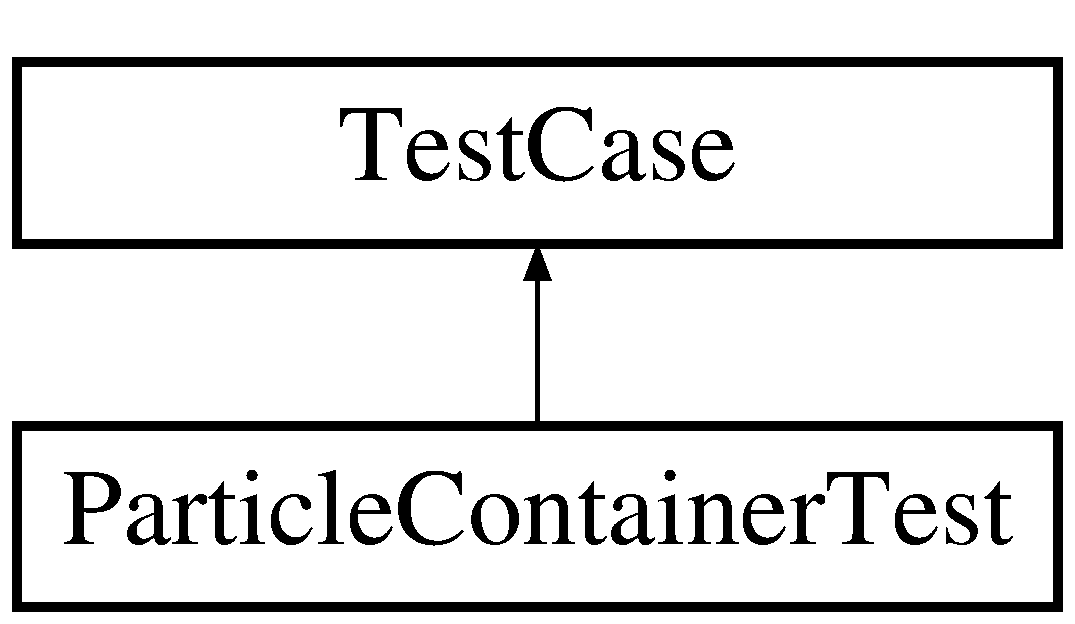
\includegraphics[height=2.000000cm]{classParticleContainerTest}
\end{center}
\end{figure}
\subsection*{Public Member Functions}
\begin{DoxyCompactItemize}
\item 
\hyperlink{classParticleContainerTest_ac9c892489b33cc0fb091eca01677f74e}{Particle\-Container\-Test} ()
\item 
virtual \hyperlink{classParticleContainerTest_a6fff30944bc8d19c2a838ac0735222fc}{$\sim$\-Particle\-Container\-Test} ()
\item 
void \hyperlink{classParticleContainerTest_a114674bf106f1237eb8e5d0afa2cead0}{set\-Up} ()
\item 
void \hyperlink{classParticleContainerTest_a3109d4eb4afad3ff4c046fc47ad4fcc4}{tear\-Down} ()
\item 
void \hyperlink{classParticleContainerTest_a4cdf950edb489d8097227db9266e7d50}{test\-Initialize} ()
\item 
void \hyperlink{classParticleContainerTest_ae720809123b33fd904ac94aa316c0614}{test\-Begin} ()
\item 
void \hyperlink{classParticleContainerTest_a2703e03485bff5309ff791701fc1c890}{test\-End} ()
\item 
void \hyperlink{classParticleContainerTest_a05b72ca03cb3f7aa141848af6710205a}{test\-Get\-List} ()
\item 
void \hyperlink{classParticleContainerTest_a51079ca20b39f6379629c6d34db08014}{test\-Size} ()
\end{DoxyCompactItemize}
\subsection*{Static Public Member Functions}
\begin{DoxyCompactItemize}
\item 
static Test $\ast$ \hyperlink{classParticleContainerTest_afd0e83c2b1690977082c11839937bcaa}{suite} ()
\end{DoxyCompactItemize}
\subsection*{Private Attributes}
\begin{DoxyCompactItemize}
\item 
\hyperlink{classutils_1_1ParticleContainer}{utils\-::\-Particle\-Container} \hyperlink{classParticleContainerTest_a609cd2f0533eb544f6e7601bbe8766dc}{container}
\item 
std\-::list$<$ \hyperlink{classParticle}{Particle} $>$ \hyperlink{classParticleContainerTest_a014875b9bbad38f13cb979be52b91e80}{particles}
\end{DoxyCompactItemize}


\subsection{Constructor \& Destructor Documentation}
\hypertarget{classParticleContainerTest_ac9c892489b33cc0fb091eca01677f74e}{\index{Particle\-Container\-Test@{Particle\-Container\-Test}!Particle\-Container\-Test@{Particle\-Container\-Test}}
\index{Particle\-Container\-Test@{Particle\-Container\-Test}!ParticleContainerTest@{Particle\-Container\-Test}}
\subsubsection[{Particle\-Container\-Test}]{\setlength{\rightskip}{0pt plus 5cm}Particle\-Container\-Test\-::\-Particle\-Container\-Test (
\begin{DoxyParamCaption}
{}
\end{DoxyParamCaption}
)}}\label{classParticleContainerTest_ac9c892489b33cc0fb091eca01677f74e}
\hypertarget{classParticleContainerTest_a6fff30944bc8d19c2a838ac0735222fc}{\index{Particle\-Container\-Test@{Particle\-Container\-Test}!$\sim$\-Particle\-Container\-Test@{$\sim$\-Particle\-Container\-Test}}
\index{$\sim$\-Particle\-Container\-Test@{$\sim$\-Particle\-Container\-Test}!ParticleContainerTest@{Particle\-Container\-Test}}
\subsubsection[{$\sim$\-Particle\-Container\-Test}]{\setlength{\rightskip}{0pt plus 5cm}Particle\-Container\-Test\-::$\sim$\-Particle\-Container\-Test (
\begin{DoxyParamCaption}
{}
\end{DoxyParamCaption}
)\hspace{0.3cm}{\ttfamily [virtual]}}}\label{classParticleContainerTest_a6fff30944bc8d19c2a838ac0735222fc}


\subsection{Member Function Documentation}
\hypertarget{classParticleContainerTest_a114674bf106f1237eb8e5d0afa2cead0}{\index{Particle\-Container\-Test@{Particle\-Container\-Test}!set\-Up@{set\-Up}}
\index{set\-Up@{set\-Up}!ParticleContainerTest@{Particle\-Container\-Test}}
\subsubsection[{set\-Up}]{\setlength{\rightskip}{0pt plus 5cm}void Particle\-Container\-Test\-::set\-Up (
\begin{DoxyParamCaption}
{}
\end{DoxyParamCaption}
)}}\label{classParticleContainerTest_a114674bf106f1237eb8e5d0afa2cead0}
Set up the test variables(container, particles) \hypertarget{classParticleContainerTest_afd0e83c2b1690977082c11839937bcaa}{\index{Particle\-Container\-Test@{Particle\-Container\-Test}!suite@{suite}}
\index{suite@{suite}!ParticleContainerTest@{Particle\-Container\-Test}}
\subsubsection[{suite}]{\setlength{\rightskip}{0pt plus 5cm}Cpp\-Unit\-::\-Test $\ast$ Particle\-Container\-Test\-::suite (
\begin{DoxyParamCaption}
{}
\end{DoxyParamCaption}
)\hspace{0.3cm}{\ttfamily [static]}}}\label{classParticleContainerTest_afd0e83c2b1690977082c11839937bcaa}
\begin{DoxyReturn}{Returns}
the Test\-Suite for the tested methods of Particle\-Container 
\end{DoxyReturn}
\hypertarget{classParticleContainerTest_a3109d4eb4afad3ff4c046fc47ad4fcc4}{\index{Particle\-Container\-Test@{Particle\-Container\-Test}!tear\-Down@{tear\-Down}}
\index{tear\-Down@{tear\-Down}!ParticleContainerTest@{Particle\-Container\-Test}}
\subsubsection[{tear\-Down}]{\setlength{\rightskip}{0pt plus 5cm}void Particle\-Container\-Test\-::tear\-Down (
\begin{DoxyParamCaption}
{}
\end{DoxyParamCaption}
)}}\label{classParticleContainerTest_a3109d4eb4afad3ff4c046fc47ad4fcc4}
\hypertarget{classParticleContainerTest_ae720809123b33fd904ac94aa316c0614}{\index{Particle\-Container\-Test@{Particle\-Container\-Test}!test\-Begin@{test\-Begin}}
\index{test\-Begin@{test\-Begin}!ParticleContainerTest@{Particle\-Container\-Test}}
\subsubsection[{test\-Begin}]{\setlength{\rightskip}{0pt plus 5cm}void Particle\-Container\-Test\-::test\-Begin (
\begin{DoxyParamCaption}
{}
\end{DoxyParamCaption}
)}}\label{classParticleContainerTest_ae720809123b33fd904ac94aa316c0614}
Check the begin() method of the Particle\-Container \hypertarget{classParticleContainerTest_a2703e03485bff5309ff791701fc1c890}{\index{Particle\-Container\-Test@{Particle\-Container\-Test}!test\-End@{test\-End}}
\index{test\-End@{test\-End}!ParticleContainerTest@{Particle\-Container\-Test}}
\subsubsection[{test\-End}]{\setlength{\rightskip}{0pt plus 5cm}void Particle\-Container\-Test\-::test\-End (
\begin{DoxyParamCaption}
{}
\end{DoxyParamCaption}
)}}\label{classParticleContainerTest_a2703e03485bff5309ff791701fc1c890}
Check the end() method of the Particle\-Container \hypertarget{classParticleContainerTest_a05b72ca03cb3f7aa141848af6710205a}{\index{Particle\-Container\-Test@{Particle\-Container\-Test}!test\-Get\-List@{test\-Get\-List}}
\index{test\-Get\-List@{test\-Get\-List}!ParticleContainerTest@{Particle\-Container\-Test}}
\subsubsection[{test\-Get\-List}]{\setlength{\rightskip}{0pt plus 5cm}void Particle\-Container\-Test\-::test\-Get\-List (
\begin{DoxyParamCaption}
{}
\end{DoxyParamCaption}
)}}\label{classParticleContainerTest_a05b72ca03cb3f7aa141848af6710205a}
Check the get\-List() method of the Particle\-Container \hypertarget{classParticleContainerTest_a4cdf950edb489d8097227db9266e7d50}{\index{Particle\-Container\-Test@{Particle\-Container\-Test}!test\-Initialize@{test\-Initialize}}
\index{test\-Initialize@{test\-Initialize}!ParticleContainerTest@{Particle\-Container\-Test}}
\subsubsection[{test\-Initialize}]{\setlength{\rightskip}{0pt plus 5cm}void Particle\-Container\-Test\-::test\-Initialize (
\begin{DoxyParamCaption}
{}
\end{DoxyParamCaption}
)}}\label{classParticleContainerTest_a4cdf950edb489d8097227db9266e7d50}
Check the initialization of the Particle\-Container \hypertarget{classParticleContainerTest_a51079ca20b39f6379629c6d34db08014}{\index{Particle\-Container\-Test@{Particle\-Container\-Test}!test\-Size@{test\-Size}}
\index{test\-Size@{test\-Size}!ParticleContainerTest@{Particle\-Container\-Test}}
\subsubsection[{test\-Size}]{\setlength{\rightskip}{0pt plus 5cm}void Particle\-Container\-Test\-::test\-Size (
\begin{DoxyParamCaption}
{}
\end{DoxyParamCaption}
)}}\label{classParticleContainerTest_a51079ca20b39f6379629c6d34db08014}
Check the size() method of the Particle\-Container 

\subsection{Member Data Documentation}
\hypertarget{classParticleContainerTest_a609cd2f0533eb544f6e7601bbe8766dc}{\index{Particle\-Container\-Test@{Particle\-Container\-Test}!container@{container}}
\index{container@{container}!ParticleContainerTest@{Particle\-Container\-Test}}
\subsubsection[{container}]{\setlength{\rightskip}{0pt plus 5cm}{\bf utils\-::\-Particle\-Container} Particle\-Container\-Test\-::container\hspace{0.3cm}{\ttfamily [private]}}}\label{classParticleContainerTest_a609cd2f0533eb544f6e7601bbe8766dc}
The particle container who will be tested \hypertarget{classParticleContainerTest_a014875b9bbad38f13cb979be52b91e80}{\index{Particle\-Container\-Test@{Particle\-Container\-Test}!particles@{particles}}
\index{particles@{particles}!ParticleContainerTest@{Particle\-Container\-Test}}
\subsubsection[{particles}]{\setlength{\rightskip}{0pt plus 5cm}std\-::list$<${\bf Particle}$>$ Particle\-Container\-Test\-::particles\hspace{0.3cm}{\ttfamily [private]}}}\label{classParticleContainerTest_a014875b9bbad38f13cb979be52b91e80}
The particle list, which will be used to compare to the container 

The documentation for this class was generated from the following files\-:\begin{DoxyCompactItemize}
\item 
src/tests/\hyperlink{ParticleContainerTest_8h}{Particle\-Container\-Test.\-h}\item 
src/tests/\hyperlink{ParticleContainerTest_8cpp}{Particle\-Container\-Test.\-cpp}\end{DoxyCompactItemize}

\hypertarget{classutils_1_1ParticleGenerator}{\section{utils\-:\-:Particle\-Generator Class Reference}
\label{classutils_1_1ParticleGenerator}\index{utils\-::\-Particle\-Generator@{utils\-::\-Particle\-Generator}}
}


This is a class capsulating (almost) all work related to cuboids and spheres.  




{\ttfamily \#include $<$Particle\-Generator.\-h$>$}

\subsection*{Public Member Functions}
\begin{DoxyCompactItemize}
\item 
\hyperlink{classutils_1_1ParticleGenerator_a66cee361b12e3294bc7a2259d401fe02}{Particle\-Generator} ()
\item 
\hyperlink{classutils_1_1ParticleGenerator_a1c12068bec5fd0df8d9a34d4bfb7f726}{Particle\-Generator} (std\-::list$<$ \hyperlink{classCuboid}{Cuboid} $>$ \&cub\-List)
\item 
\hyperlink{classutils_1_1ParticleGenerator_a0eba44befd40227a167f9f562d718515}{Particle\-Generator} (std\-::list$<$ \hyperlink{classParticle}{Particle} $>$ \&par\-List)
\item 
\hyperlink{classutils_1_1ParticleGenerator_ac9560217a90a901d9a65247028468106}{Particle\-Generator} (std\-::list$<$ \hyperlink{classSphere}{Sphere} $>$ \&sph\-List)
\item 
void \hyperlink{classutils_1_1ParticleGenerator_a405c1b60bfbd08c2c31fefb927290945}{read\-Cuboids} (char $\ast$filename)
\item 
void \hyperlink{classutils_1_1ParticleGenerator_a47095ba94d78941e9ce4f08b25fccc33}{extract\-Setting} (std\-::string filename, double \&\hyperlink{MolSim_8cpp_a00b0c9b1c3ea8bb73a7fc8b53a3961fd}{start\-\_\-time}, double \&\hyperlink{MolSim_8cpp_a8c7ea5e69ce954c1d81db1732f9f426a}{end\-\_\-time}, double \&\hyperlink{MolSim_8cpp_a4cfc079302fe9a34fe24637c4e44303a}{delta\-\_\-t}, std\-::list$<$ string $>$ \&\hyperlink{MolSim_8cpp_a448cf355949f9675fa5f3d5599923d75}{input\-Names}, std\-::list$<$ string $>$ \&\hyperlink{MolSim_8cpp_ad5280d724148f1f34eb9e36fba1e9bf1}{input\-Types}, string \&\hyperlink{MolSim_8cpp_ac7d2734291385dce3211bcb0884021c1}{output\-Mask}, int \&output\-Freq, \hyperlink{classutils_1_1Vector}{utils\-::\-Vector}$<$ double, 3 $>$ \&\hyperlink{MolSim_8cpp_a62ca172a74e96becbd5ebbae3052bbd3}{domain\-Size}, double \&r\-\_\-cutoff, std\-::vector$<$ int $>$ \&domain\-Bound\-Cond, double \&g\-\_\-const, int \&\hyperlink{MolSim_8cpp_ad255f675bdb1dcbda2160670f9912985}{input\-Size})
\item 
void \hyperlink{classutils_1_1ParticleGenerator_a5b99fee3ef17845bff2ef6ed4e8f9d04}{extract\-Particles} (const string filename)
\item 
void \hyperlink{classutils_1_1ParticleGenerator_addad87e40dc0c5d49e5df4533121771d}{extract\-Cuboids} (const string filename)
\item 
void \hyperlink{classutils_1_1ParticleGenerator_a93d2efd2781548606dc52f4a6ab3ca57}{extract\-Spheres} (const string filename)
\item 
void \hyperlink{classutils_1_1ParticleGenerator_a89a4177490575ae9486e0eaecdb52dfd}{cuboids\-To\-List} ()
\item 
void \hyperlink{classutils_1_1ParticleGenerator_a2ea629339cda550d6daae10ec339296e}{spheres\-To\-List} ()
\item 
void \hyperlink{classutils_1_1ParticleGenerator_a7048e1fc122f6e5e962f23071031a0e0}{merge\-With\-Particle\-List} (std\-::list$<$ \hyperlink{classParticle}{Particle} $>$ \&before)
\item 
std\-::list$<$ \hyperlink{classCuboid}{Cuboid} $>$ \& \hyperlink{classutils_1_1ParticleGenerator_ad8da4620c020650970252213333b939e}{get\-Cuboid\-List} ()
\item 
std\-::list$<$ \hyperlink{classSphere}{Sphere} $>$ \& \hyperlink{classutils_1_1ParticleGenerator_a50edacf6ec960526e5182aaa5e62a192}{get\-Sphere\-List} ()
\item 
std\-::list$<$ \hyperlink{classParticle}{Particle} $>$ \& \hyperlink{classutils_1_1ParticleGenerator_a59ad1749a839f3e89e58d3f92ec94b4f}{get\-Particle\-List} ()
\item 
virtual \hyperlink{classutils_1_1ParticleGenerator_a37a629906f87d7200989d6bb2dff796d}{$\sim$\-Particle\-Generator} ()
\end{DoxyCompactItemize}
\subsection*{Private Attributes}
\begin{DoxyCompactItemize}
\item 
std\-::list$<$ \hyperlink{classCuboid}{Cuboid} $>$ \hyperlink{classutils_1_1ParticleGenerator_a2b4d4491fa74e20a23f7affc96de834a}{cuboid\-List}
\item 
std\-::list$<$ \hyperlink{classSphere}{Sphere} $>$ \hyperlink{classutils_1_1ParticleGenerator_a51b9b7685b429b44bd889a9b62b25ec2}{sphere\-List}
\item 
std\-::list$<$ \hyperlink{classParticle}{Particle} $>$ \hyperlink{classutils_1_1ParticleGenerator_a83e8886303b0e6d0e1b269cb54e7d04b}{particle\-List}
\end{DoxyCompactItemize}


\subsection{Detailed Description}
This is a class capsulating (almost) all work related to cuboids and spheres. 

A particle generator contains a list of cuboids/spheres and is therefore able to initialize a set of particles into cuboids/spheres. Extracting needed information from an output file into cuboids/spheres and converting cuboids/spheres into one single list of particles are possible in this class. 

\subsection{Constructor \& Destructor Documentation}
\hypertarget{classutils_1_1ParticleGenerator_a66cee361b12e3294bc7a2259d401fe02}{\index{utils\-::\-Particle\-Generator@{utils\-::\-Particle\-Generator}!Particle\-Generator@{Particle\-Generator}}
\index{Particle\-Generator@{Particle\-Generator}!utils::ParticleGenerator@{utils\-::\-Particle\-Generator}}
\subsubsection[{Particle\-Generator}]{\setlength{\rightskip}{0pt plus 5cm}Particle\-Generator\-::\-Particle\-Generator (
\begin{DoxyParamCaption}
{}
\end{DoxyParamCaption}
)}}\label{classutils_1_1ParticleGenerator_a66cee361b12e3294bc7a2259d401fe02}
Default constructor. \hypertarget{classutils_1_1ParticleGenerator_a1c12068bec5fd0df8d9a34d4bfb7f726}{\index{utils\-::\-Particle\-Generator@{utils\-::\-Particle\-Generator}!Particle\-Generator@{Particle\-Generator}}
\index{Particle\-Generator@{Particle\-Generator}!utils::ParticleGenerator@{utils\-::\-Particle\-Generator}}
\subsubsection[{Particle\-Generator}]{\setlength{\rightskip}{0pt plus 5cm}Particle\-Generator\-::\-Particle\-Generator (
\begin{DoxyParamCaption}
\item[{std\-::list$<$ {\bf Cuboid} $>$ \&}]{cub\-List}
\end{DoxyParamCaption}
)}}\label{classutils_1_1ParticleGenerator_a1c12068bec5fd0df8d9a34d4bfb7f726}
Main cuboid constructor, which creates a particle generator from a list of cuboids. 
\begin{DoxyParams}[1]{Parameters}
\mbox{\tt in}  & {\em cub\-List} & A list of cuboids. \\
\hline
\end{DoxyParams}
\hypertarget{classutils_1_1ParticleGenerator_a0eba44befd40227a167f9f562d718515}{\index{utils\-::\-Particle\-Generator@{utils\-::\-Particle\-Generator}!Particle\-Generator@{Particle\-Generator}}
\index{Particle\-Generator@{Particle\-Generator}!utils::ParticleGenerator@{utils\-::\-Particle\-Generator}}
\subsubsection[{Particle\-Generator}]{\setlength{\rightskip}{0pt plus 5cm}Particle\-Generator\-::\-Particle\-Generator (
\begin{DoxyParamCaption}
\item[{std\-::list$<$ {\bf Particle} $>$ \&}]{par\-List}
\end{DoxyParamCaption}
)}}\label{classutils_1_1ParticleGenerator_a0eba44befd40227a167f9f562d718515}
Main particle constructor, which creates a particle generator from a list of untructered particles. 
\begin{DoxyParams}[1]{Parameters}
\mbox{\tt in}  & {\em par\-List} & A list of particles. \\
\hline
\end{DoxyParams}
\hypertarget{classutils_1_1ParticleGenerator_ac9560217a90a901d9a65247028468106}{\index{utils\-::\-Particle\-Generator@{utils\-::\-Particle\-Generator}!Particle\-Generator@{Particle\-Generator}}
\index{Particle\-Generator@{Particle\-Generator}!utils::ParticleGenerator@{utils\-::\-Particle\-Generator}}
\subsubsection[{Particle\-Generator}]{\setlength{\rightskip}{0pt plus 5cm}Particle\-Generator\-::\-Particle\-Generator (
\begin{DoxyParamCaption}
\item[{std\-::list$<$ {\bf Sphere} $>$ \&}]{sph\-List}
\end{DoxyParamCaption}
)}}\label{classutils_1_1ParticleGenerator_ac9560217a90a901d9a65247028468106}
Main sphere constructor, which creates a particle generator from a list of spheres. 
\begin{DoxyParams}[1]{Parameters}
\mbox{\tt in}  & {\em sph\-List} & A list of spheres. \\
\hline
\end{DoxyParams}
\hypertarget{classutils_1_1ParticleGenerator_a37a629906f87d7200989d6bb2dff796d}{\index{utils\-::\-Particle\-Generator@{utils\-::\-Particle\-Generator}!$\sim$\-Particle\-Generator@{$\sim$\-Particle\-Generator}}
\index{$\sim$\-Particle\-Generator@{$\sim$\-Particle\-Generator}!utils::ParticleGenerator@{utils\-::\-Particle\-Generator}}
\subsubsection[{$\sim$\-Particle\-Generator}]{\setlength{\rightskip}{0pt plus 5cm}Particle\-Generator\-::$\sim$\-Particle\-Generator (
\begin{DoxyParamCaption}
{}
\end{DoxyParamCaption}
)\hspace{0.3cm}{\ttfamily [virtual]}}}\label{classutils_1_1ParticleGenerator_a37a629906f87d7200989d6bb2dff796d}


\subsection{Member Function Documentation}
\hypertarget{classutils_1_1ParticleGenerator_a89a4177490575ae9486e0eaecdb52dfd}{\index{utils\-::\-Particle\-Generator@{utils\-::\-Particle\-Generator}!cuboids\-To\-List@{cuboids\-To\-List}}
\index{cuboids\-To\-List@{cuboids\-To\-List}!utils::ParticleGenerator@{utils\-::\-Particle\-Generator}}
\subsubsection[{cuboids\-To\-List}]{\setlength{\rightskip}{0pt plus 5cm}void Particle\-Generator\-::cuboids\-To\-List (
\begin{DoxyParamCaption}
{}
\end{DoxyParamCaption}
)}}\label{classutils_1_1ParticleGenerator_a89a4177490575ae9486e0eaecdb52dfd}
Converts particle generator's list of cuboids into one single list of particles. 
\begin{DoxyParams}[1]{Parameters}
\mbox{\tt out}  & {\em particle\-List} & The result will be stored here. \\
\hline
\end{DoxyParams}
\hypertarget{classutils_1_1ParticleGenerator_addad87e40dc0c5d49e5df4533121771d}{\index{utils\-::\-Particle\-Generator@{utils\-::\-Particle\-Generator}!extract\-Cuboids@{extract\-Cuboids}}
\index{extract\-Cuboids@{extract\-Cuboids}!utils::ParticleGenerator@{utils\-::\-Particle\-Generator}}
\subsubsection[{extract\-Cuboids}]{\setlength{\rightskip}{0pt plus 5cm}void Particle\-Generator\-::extract\-Cuboids (
\begin{DoxyParamCaption}
\item[{const string}]{filename}
\end{DoxyParamCaption}
)}}\label{classutils_1_1ParticleGenerator_addad87e40dc0c5d49e5df4533121771d}
The reading procedure, which can convert information from a given X\-M\-L input file into particle generator's list of cuboids.


\begin{DoxyParams}[1]{Parameters}
\mbox{\tt in}  & {\em filename} & Name of the input file (e.\-g\-: \char`\"{}\-Input\-Cuboids.\-xml\char`\"{}). \\
\hline
\mbox{\tt out}  & {\em cub\-List} & The cuboids will be stored here. \\
\hline
\end{DoxyParams}
\hypertarget{classutils_1_1ParticleGenerator_a5b99fee3ef17845bff2ef6ed4e8f9d04}{\index{utils\-::\-Particle\-Generator@{utils\-::\-Particle\-Generator}!extract\-Particles@{extract\-Particles}}
\index{extract\-Particles@{extract\-Particles}!utils::ParticleGenerator@{utils\-::\-Particle\-Generator}}
\subsubsection[{extract\-Particles}]{\setlength{\rightskip}{0pt plus 5cm}void Particle\-Generator\-::extract\-Particles (
\begin{DoxyParamCaption}
\item[{const string}]{filename}
\end{DoxyParamCaption}
)}}\label{classutils_1_1ParticleGenerator_a5b99fee3ef17845bff2ef6ed4e8f9d04}
The reading procedure, which can convert information from a given X\-M\-L input file into particle generator's list of unstructered particles.


\begin{DoxyParams}[1]{Parameters}
\mbox{\tt in}  & {\em filename} & Name of the input file (e.\-g\-: \char`\"{}\-Input\-Particles.\-xml\char`\"{}). \\
\hline
\mbox{\tt out}  & {\em particle\-List} & The particles will be stored here. \\
\hline
\end{DoxyParams}
\hypertarget{classutils_1_1ParticleGenerator_a47095ba94d78941e9ce4f08b25fccc33}{\index{utils\-::\-Particle\-Generator@{utils\-::\-Particle\-Generator}!extract\-Setting@{extract\-Setting}}
\index{extract\-Setting@{extract\-Setting}!utils::ParticleGenerator@{utils\-::\-Particle\-Generator}}
\subsubsection[{extract\-Setting}]{\setlength{\rightskip}{0pt plus 5cm}void Particle\-Generator\-::extract\-Setting (
\begin{DoxyParamCaption}
\item[{std\-::string}]{filename, }
\item[{double \&}]{start\-\_\-time, }
\item[{double \&}]{end\-\_\-time, }
\item[{double \&}]{delta\-\_\-t, }
\item[{std\-::list$<$ string $>$ \&}]{input\-Names, }
\item[{std\-::list$<$ string $>$ \&}]{input\-Types, }
\item[{string \&}]{output\-Mask, }
\item[{int \&}]{output\-Freq, }
\item[{{\bf utils\-::\-Vector}$<$ double, 3 $>$ \&}]{domain\-Size, }
\item[{double \&}]{r\-\_\-cutoff, }
\item[{std\-::vector$<$ int $>$ \&}]{domain\-Bound\-Cond, }
\item[{double \&}]{g\-\_\-const, }
\item[{int \&}]{input\-Size}
\end{DoxyParamCaption}
)}}\label{classutils_1_1ParticleGenerator_a47095ba94d78941e9ce4f08b25fccc33}
The reading procedure, which can extract all information needed for configuring the simulation from a given X\-M\-L input file .


\begin{DoxyParams}[1]{Parameters}
\mbox{\tt in}  & {\em filename} & Input file name. \\
\hline
\mbox{\tt out}  & {\em start\-\_\-time} & Start time of simulation will be stored here. \\
\hline
\mbox{\tt out}  & {\em end\-\_\-time} & End time of simulation will be stored here. \\
\hline
\mbox{\tt out}  & {\em delta\-\_\-t} & Delta time (between 2 iterations) of simulation will be stored here. \\
\hline
\mbox{\tt out}  & {\em input\-Names} & A list of X\-M\-L input names, which will be extracted. \\
\hline
\mbox{\tt out}  & {\em input\-Types} & A list of types each X\-M\-L input name has (\char`\"{}cuboids\char`\"{}/\char`\"{}spheres\char`\"{}). \\
\hline
\mbox{\tt out}  & {\em output\-Mask} & Output files will named after this mask. \\
\hline
\mbox{\tt out}  & {\em output\-Freq} & How many iterations it takes to write an output file. \\
\hline
\mbox{\tt out}  & {\em domain\-Size} & A 3\-D vector indicating size of the domain (Linked Cell Algorithm). \\
\hline
\mbox{\tt out}  & {\em r\-\_\-cutoff} & Cutoff radius (Short Range Algorithm). \\
\hline
\mbox{\tt out}  & {\em domain\-Bound\-Cond} & Saves boundary conditions (\char`\"{}outflow\char`\"{}/\char`\"{}reflecting\char`\"{}) for 6 sides of domain. \\
\hline
\mbox{\tt out}  & {\em g\-\_\-const} & The constant g of gravitational force \\
\hline
\mbox{\tt out}  & {\em input\-Size} & Number of particle types \\
\hline
\end{DoxyParams}
\hypertarget{classutils_1_1ParticleGenerator_a93d2efd2781548606dc52f4a6ab3ca57}{\index{utils\-::\-Particle\-Generator@{utils\-::\-Particle\-Generator}!extract\-Spheres@{extract\-Spheres}}
\index{extract\-Spheres@{extract\-Spheres}!utils::ParticleGenerator@{utils\-::\-Particle\-Generator}}
\subsubsection[{extract\-Spheres}]{\setlength{\rightskip}{0pt plus 5cm}void Particle\-Generator\-::extract\-Spheres (
\begin{DoxyParamCaption}
\item[{const string}]{filename}
\end{DoxyParamCaption}
)}}\label{classutils_1_1ParticleGenerator_a93d2efd2781548606dc52f4a6ab3ca57}
The reading procedure, which can convert information from a given X\-M\-L input file into particle generator's list of spheres.


\begin{DoxyParams}[1]{Parameters}
\mbox{\tt in}  & {\em filename} & Name of the input file (e.\-g\-: \char`\"{}\-Input\-Spheres.\-xml\char`\"{}). \\
\hline
\mbox{\tt out}  & {\em sph\-List} & The spheres will be stored here. \\
\hline
\end{DoxyParams}
\hypertarget{classutils_1_1ParticleGenerator_ad8da4620c020650970252213333b939e}{\index{utils\-::\-Particle\-Generator@{utils\-::\-Particle\-Generator}!get\-Cuboid\-List@{get\-Cuboid\-List}}
\index{get\-Cuboid\-List@{get\-Cuboid\-List}!utils::ParticleGenerator@{utils\-::\-Particle\-Generator}}
\subsubsection[{get\-Cuboid\-List}]{\setlength{\rightskip}{0pt plus 5cm}std\-::list$<$ {\bf Cuboid} $>$ \& Particle\-Generator\-::get\-Cuboid\-List (
\begin{DoxyParamCaption}
{}
\end{DoxyParamCaption}
)}}\label{classutils_1_1ParticleGenerator_ad8da4620c020650970252213333b939e}
\begin{DoxyReturn}{Returns}
\hyperlink{classParticle}{Particle} generator's list of cuboids. 
\end{DoxyReturn}
\hypertarget{classutils_1_1ParticleGenerator_a59ad1749a839f3e89e58d3f92ec94b4f}{\index{utils\-::\-Particle\-Generator@{utils\-::\-Particle\-Generator}!get\-Particle\-List@{get\-Particle\-List}}
\index{get\-Particle\-List@{get\-Particle\-List}!utils::ParticleGenerator@{utils\-::\-Particle\-Generator}}
\subsubsection[{get\-Particle\-List}]{\setlength{\rightskip}{0pt plus 5cm}std\-::list$<$ {\bf Particle} $>$ \& Particle\-Generator\-::get\-Particle\-List (
\begin{DoxyParamCaption}
{}
\end{DoxyParamCaption}
)}}\label{classutils_1_1ParticleGenerator_a59ad1749a839f3e89e58d3f92ec94b4f}
\begin{DoxyReturn}{Returns}
\hyperlink{classParticle}{Particle} generator's list of particles. 
\end{DoxyReturn}
\hypertarget{classutils_1_1ParticleGenerator_a50edacf6ec960526e5182aaa5e62a192}{\index{utils\-::\-Particle\-Generator@{utils\-::\-Particle\-Generator}!get\-Sphere\-List@{get\-Sphere\-List}}
\index{get\-Sphere\-List@{get\-Sphere\-List}!utils::ParticleGenerator@{utils\-::\-Particle\-Generator}}
\subsubsection[{get\-Sphere\-List}]{\setlength{\rightskip}{0pt plus 5cm}std\-::list$<$ {\bf Sphere} $>$ \& Particle\-Generator\-::get\-Sphere\-List (
\begin{DoxyParamCaption}
{}
\end{DoxyParamCaption}
)}}\label{classutils_1_1ParticleGenerator_a50edacf6ec960526e5182aaa5e62a192}
\begin{DoxyReturn}{Returns}
\hyperlink{classParticle}{Particle} generator's list of spheres. 
\end{DoxyReturn}
\hypertarget{classutils_1_1ParticleGenerator_a7048e1fc122f6e5e962f23071031a0e0}{\index{utils\-::\-Particle\-Generator@{utils\-::\-Particle\-Generator}!merge\-With\-Particle\-List@{merge\-With\-Particle\-List}}
\index{merge\-With\-Particle\-List@{merge\-With\-Particle\-List}!utils::ParticleGenerator@{utils\-::\-Particle\-Generator}}
\subsubsection[{merge\-With\-Particle\-List}]{\setlength{\rightskip}{0pt plus 5cm}void Particle\-Generator\-::merge\-With\-Particle\-List (
\begin{DoxyParamCaption}
\item[{std\-::list$<$ {\bf Particle} $>$ \&}]{before}
\end{DoxyParamCaption}
)}}\label{classutils_1_1ParticleGenerator_a7048e1fc122f6e5e962f23071031a0e0}
Merge with a given list, which will stand B\-E\-F\-O\-R\-E particle\-List. 
\begin{DoxyParams}[1]{Parameters}
\mbox{\tt in}  & {\em before} & This list will be merged. \\
\hline
\mbox{\tt in}  & {\em particle\-List} & All elements of this list will be added into the gear side of before. \\
\hline
\mbox{\tt out}  & {\em before} & The new elements will be pushed into before's back. \\
\hline
\end{DoxyParams}
\hypertarget{classutils_1_1ParticleGenerator_a405c1b60bfbd08c2c31fefb927290945}{\index{utils\-::\-Particle\-Generator@{utils\-::\-Particle\-Generator}!read\-Cuboids@{read\-Cuboids}}
\index{read\-Cuboids@{read\-Cuboids}!utils::ParticleGenerator@{utils\-::\-Particle\-Generator}}
\subsubsection[{read\-Cuboids}]{\setlength{\rightskip}{0pt plus 5cm}void Particle\-Generator\-::read\-Cuboids (
\begin{DoxyParamCaption}
\item[{char $\ast$}]{filename}
\end{DoxyParamCaption}
)}}\label{classutils_1_1ParticleGenerator_a405c1b60bfbd08c2c31fefb927290945}
The reading procedure, which can convert information from a given T\-X\-T input file into particle generator's list of cuboids.


\begin{DoxyParams}[1]{Parameters}
\mbox{\tt in}  & {\em filename} & Name of the input file (e.\-g\-: \char`\"{}eingabe-\/brownian.\-txt\char`\"{}). \\
\hline
\mbox{\tt out}  & {\em cub\-List} & The cuboids will be stored here. \\
\hline
\end{DoxyParams}
\hypertarget{classutils_1_1ParticleGenerator_a2ea629339cda550d6daae10ec339296e}{\index{utils\-::\-Particle\-Generator@{utils\-::\-Particle\-Generator}!spheres\-To\-List@{spheres\-To\-List}}
\index{spheres\-To\-List@{spheres\-To\-List}!utils::ParticleGenerator@{utils\-::\-Particle\-Generator}}
\subsubsection[{spheres\-To\-List}]{\setlength{\rightskip}{0pt plus 5cm}void Particle\-Generator\-::spheres\-To\-List (
\begin{DoxyParamCaption}
{}
\end{DoxyParamCaption}
)}}\label{classutils_1_1ParticleGenerator_a2ea629339cda550d6daae10ec339296e}
Converts particle generator's list of spheres into one single list of particles. 
\begin{DoxyParams}[1]{Parameters}
\mbox{\tt out}  & {\em particle\-List} & The result will be stored here. \\
\hline
\end{DoxyParams}


\subsection{Member Data Documentation}
\hypertarget{classutils_1_1ParticleGenerator_a2b4d4491fa74e20a23f7affc96de834a}{\index{utils\-::\-Particle\-Generator@{utils\-::\-Particle\-Generator}!cuboid\-List@{cuboid\-List}}
\index{cuboid\-List@{cuboid\-List}!utils::ParticleGenerator@{utils\-::\-Particle\-Generator}}
\subsubsection[{cuboid\-List}]{\setlength{\rightskip}{0pt plus 5cm}std\-::list$<${\bf Cuboid}$>$ utils\-::\-Particle\-Generator\-::cuboid\-List\hspace{0.3cm}{\ttfamily [private]}}}\label{classutils_1_1ParticleGenerator_a2b4d4491fa74e20a23f7affc96de834a}
A list of cuboids, each cuboid is an instance of class \hyperlink{classCuboid}{Cuboid}. \hypertarget{classutils_1_1ParticleGenerator_a83e8886303b0e6d0e1b269cb54e7d04b}{\index{utils\-::\-Particle\-Generator@{utils\-::\-Particle\-Generator}!particle\-List@{particle\-List}}
\index{particle\-List@{particle\-List}!utils::ParticleGenerator@{utils\-::\-Particle\-Generator}}
\subsubsection[{particle\-List}]{\setlength{\rightskip}{0pt plus 5cm}std\-::list$<${\bf Particle}$>$ utils\-::\-Particle\-Generator\-::particle\-List\hspace{0.3cm}{\ttfamily [private]}}}\label{classutils_1_1ParticleGenerator_a83e8886303b0e6d0e1b269cb54e7d04b}
The particles of either cuboids or spheres will be stored here. \hypertarget{classutils_1_1ParticleGenerator_a51b9b7685b429b44bd889a9b62b25ec2}{\index{utils\-::\-Particle\-Generator@{utils\-::\-Particle\-Generator}!sphere\-List@{sphere\-List}}
\index{sphere\-List@{sphere\-List}!utils::ParticleGenerator@{utils\-::\-Particle\-Generator}}
\subsubsection[{sphere\-List}]{\setlength{\rightskip}{0pt plus 5cm}std\-::list$<${\bf Sphere}$>$ utils\-::\-Particle\-Generator\-::sphere\-List\hspace{0.3cm}{\ttfamily [private]}}}\label{classutils_1_1ParticleGenerator_a51b9b7685b429b44bd889a9b62b25ec2}
A list of spheres, each sphere is an instance of class \hyperlink{classSphere}{Sphere}. 

The documentation for this class was generated from the following files\-:\begin{DoxyCompactItemize}
\item 
src/utils/\hyperlink{ParticleGenerator_8h}{Particle\-Generator.\-h}\item 
src/utils/\hyperlink{ParticleGenerator_8cpp}{Particle\-Generator.\-cpp}\end{DoxyCompactItemize}

\hypertarget{classParticleGeneratorTest}{\section{Particle\-Generator\-Test Class Reference}
\label{classParticleGeneratorTest}\index{Particle\-Generator\-Test@{Particle\-Generator\-Test}}
}


{\ttfamily \#include $<$Particle\-Generator\-Test.\-h$>$}

Inheritance diagram for Particle\-Generator\-Test\-:\begin{figure}[H]
\begin{center}
\leavevmode
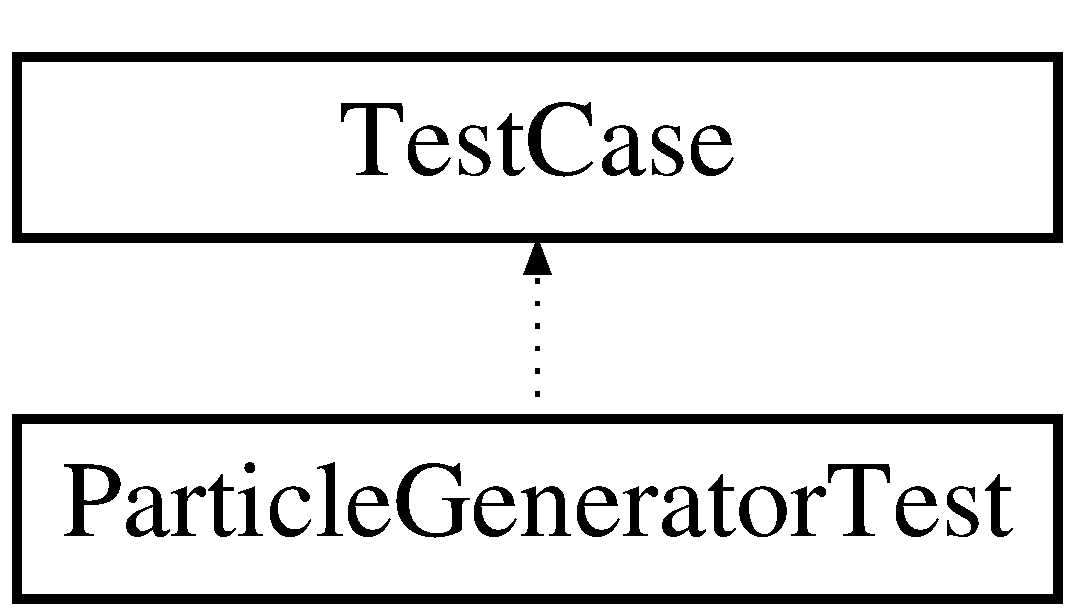
\includegraphics[height=2.000000cm]{classParticleGeneratorTest}
\end{center}
\end{figure}
\subsection*{Public Member Functions}
\begin{DoxyCompactItemize}
\item 
\hyperlink{classParticleGeneratorTest_af27d139a180f3d07501c726069abac48}{Particle\-Generator\-Test} ()
\item 
virtual \hyperlink{classParticleGeneratorTest_a2882f3ae2508ac7541649ad0445f76e6}{$\sim$\-Particle\-Generator\-Test} ()
\item 
void \hyperlink{classParticleGeneratorTest_a5c5c45fa56773e0218ba9f827f7e78ca}{set\-Up} ()
\item 
void \hyperlink{classParticleGeneratorTest_a69d4bc5f9c69e3c6f34e0c3af750aa94}{tear\-Down} ()
\item 
void \hyperlink{classParticleGeneratorTest_a4c1fd9d420494447ea32d17c36247c1e}{test\-Read\-Cuboids} ()
\item 
void \hyperlink{classParticleGeneratorTest_af39387b0fc5449917c9388333a0b4383}{test\-Extract\-Spheres} ()
\item 
void \hyperlink{classParticleGeneratorTest_a32f14ce21a6f77874bbc9de88cd86fce}{test\-Extract\-Cuboids} ()
\item 
void \hyperlink{classParticleGeneratorTest_ae29a8a4fa5da0d37a0d5aef7f695cb58}{test\-Extract\-Particles} ()
\item 
void \hyperlink{classParticleGeneratorTest_a10a24cc68339e370d55e86037383b7bc}{test\-Extract\-Setting} ()
\end{DoxyCompactItemize}
\subsection*{Static Public Member Functions}
\begin{DoxyCompactItemize}
\item 
static Test $\ast$ \hyperlink{classParticleGeneratorTest_a6e465362e2f21d140ea4503ae32b1ae0}{suite} ()
\end{DoxyCompactItemize}
\subsection*{Private Attributes}
\begin{DoxyCompactItemize}
\item 
\hyperlink{classutils_1_1ParticleGenerator}{utils\-::\-Particle\-Generator} \hyperlink{classParticleGeneratorTest_aa0fec238220560bf0b45a14cbb6d953d}{generator}
\end{DoxyCompactItemize}


\subsection{Constructor \& Destructor Documentation}
\hypertarget{classParticleGeneratorTest_af27d139a180f3d07501c726069abac48}{\index{Particle\-Generator\-Test@{Particle\-Generator\-Test}!Particle\-Generator\-Test@{Particle\-Generator\-Test}}
\index{Particle\-Generator\-Test@{Particle\-Generator\-Test}!ParticleGeneratorTest@{Particle\-Generator\-Test}}
\subsubsection[{Particle\-Generator\-Test}]{\setlength{\rightskip}{0pt plus 5cm}Particle\-Generator\-Test\-::\-Particle\-Generator\-Test (
\begin{DoxyParamCaption}
{}
\end{DoxyParamCaption}
)}}\label{classParticleGeneratorTest_af27d139a180f3d07501c726069abac48}
\hypertarget{classParticleGeneratorTest_a2882f3ae2508ac7541649ad0445f76e6}{\index{Particle\-Generator\-Test@{Particle\-Generator\-Test}!$\sim$\-Particle\-Generator\-Test@{$\sim$\-Particle\-Generator\-Test}}
\index{$\sim$\-Particle\-Generator\-Test@{$\sim$\-Particle\-Generator\-Test}!ParticleGeneratorTest@{Particle\-Generator\-Test}}
\subsubsection[{$\sim$\-Particle\-Generator\-Test}]{\setlength{\rightskip}{0pt plus 5cm}Particle\-Generator\-Test\-::$\sim$\-Particle\-Generator\-Test (
\begin{DoxyParamCaption}
{}
\end{DoxyParamCaption}
)\hspace{0.3cm}{\ttfamily [virtual]}}}\label{classParticleGeneratorTest_a2882f3ae2508ac7541649ad0445f76e6}


\subsection{Member Function Documentation}
\hypertarget{classParticleGeneratorTest_a5c5c45fa56773e0218ba9f827f7e78ca}{\index{Particle\-Generator\-Test@{Particle\-Generator\-Test}!set\-Up@{set\-Up}}
\index{set\-Up@{set\-Up}!ParticleGeneratorTest@{Particle\-Generator\-Test}}
\subsubsection[{set\-Up}]{\setlength{\rightskip}{0pt plus 5cm}void Particle\-Generator\-Test\-::set\-Up (
\begin{DoxyParamCaption}
{}
\end{DoxyParamCaption}
)}}\label{classParticleGeneratorTest_a5c5c45fa56773e0218ba9f827f7e78ca}
Set up the two cuboids and the 3 tested particles \hypertarget{classParticleGeneratorTest_a6e465362e2f21d140ea4503ae32b1ae0}{\index{Particle\-Generator\-Test@{Particle\-Generator\-Test}!suite@{suite}}
\index{suite@{suite}!ParticleGeneratorTest@{Particle\-Generator\-Test}}
\subsubsection[{suite}]{\setlength{\rightskip}{0pt plus 5cm}Cpp\-Unit\-::\-Test $\ast$ Particle\-Generator\-Test\-::suite (
\begin{DoxyParamCaption}
{}
\end{DoxyParamCaption}
)\hspace{0.3cm}{\ttfamily [static]}}}\label{classParticleGeneratorTest_a6e465362e2f21d140ea4503ae32b1ae0}
\begin{DoxyReturn}{Returns}
the Test\-Suite for the tested methods of Particle\-Generator 
\end{DoxyReturn}
\hypertarget{classParticleGeneratorTest_a69d4bc5f9c69e3c6f34e0c3af750aa94}{\index{Particle\-Generator\-Test@{Particle\-Generator\-Test}!tear\-Down@{tear\-Down}}
\index{tear\-Down@{tear\-Down}!ParticleGeneratorTest@{Particle\-Generator\-Test}}
\subsubsection[{tear\-Down}]{\setlength{\rightskip}{0pt plus 5cm}void Particle\-Generator\-Test\-::tear\-Down (
\begin{DoxyParamCaption}
{}
\end{DoxyParamCaption}
)}}\label{classParticleGeneratorTest_a69d4bc5f9c69e3c6f34e0c3af750aa94}
\hypertarget{classParticleGeneratorTest_a32f14ce21a6f77874bbc9de88cd86fce}{\index{Particle\-Generator\-Test@{Particle\-Generator\-Test}!test\-Extract\-Cuboids@{test\-Extract\-Cuboids}}
\index{test\-Extract\-Cuboids@{test\-Extract\-Cuboids}!ParticleGeneratorTest@{Particle\-Generator\-Test}}
\subsubsection[{test\-Extract\-Cuboids}]{\setlength{\rightskip}{0pt plus 5cm}void Particle\-Generator\-Test\-::test\-Extract\-Cuboids (
\begin{DoxyParamCaption}
{}
\end{DoxyParamCaption}
)}}\label{classParticleGeneratorTest_a32f14ce21a6f77874bbc9de88cd86fce}
\hypertarget{classParticleGeneratorTest_ae29a8a4fa5da0d37a0d5aef7f695cb58}{\index{Particle\-Generator\-Test@{Particle\-Generator\-Test}!test\-Extract\-Particles@{test\-Extract\-Particles}}
\index{test\-Extract\-Particles@{test\-Extract\-Particles}!ParticleGeneratorTest@{Particle\-Generator\-Test}}
\subsubsection[{test\-Extract\-Particles}]{\setlength{\rightskip}{0pt plus 5cm}void Particle\-Generator\-Test\-::test\-Extract\-Particles (
\begin{DoxyParamCaption}
{}
\end{DoxyParamCaption}
)}}\label{classParticleGeneratorTest_ae29a8a4fa5da0d37a0d5aef7f695cb58}
\hypertarget{classParticleGeneratorTest_a10a24cc68339e370d55e86037383b7bc}{\index{Particle\-Generator\-Test@{Particle\-Generator\-Test}!test\-Extract\-Setting@{test\-Extract\-Setting}}
\index{test\-Extract\-Setting@{test\-Extract\-Setting}!ParticleGeneratorTest@{Particle\-Generator\-Test}}
\subsubsection[{test\-Extract\-Setting}]{\setlength{\rightskip}{0pt plus 5cm}void Particle\-Generator\-Test\-::test\-Extract\-Setting (
\begin{DoxyParamCaption}
{}
\end{DoxyParamCaption}
)}}\label{classParticleGeneratorTest_a10a24cc68339e370d55e86037383b7bc}
\hypertarget{classParticleGeneratorTest_af39387b0fc5449917c9388333a0b4383}{\index{Particle\-Generator\-Test@{Particle\-Generator\-Test}!test\-Extract\-Spheres@{test\-Extract\-Spheres}}
\index{test\-Extract\-Spheres@{test\-Extract\-Spheres}!ParticleGeneratorTest@{Particle\-Generator\-Test}}
\subsubsection[{test\-Extract\-Spheres}]{\setlength{\rightskip}{0pt plus 5cm}void Particle\-Generator\-Test\-::test\-Extract\-Spheres (
\begin{DoxyParamCaption}
{}
\end{DoxyParamCaption}
)}}\label{classParticleGeneratorTest_af39387b0fc5449917c9388333a0b4383}
\hypertarget{classParticleGeneratorTest_a4c1fd9d420494447ea32d17c36247c1e}{\index{Particle\-Generator\-Test@{Particle\-Generator\-Test}!test\-Read\-Cuboids@{test\-Read\-Cuboids}}
\index{test\-Read\-Cuboids@{test\-Read\-Cuboids}!ParticleGeneratorTest@{Particle\-Generator\-Test}}
\subsubsection[{test\-Read\-Cuboids}]{\setlength{\rightskip}{0pt plus 5cm}void Particle\-Generator\-Test\-::test\-Read\-Cuboids (
\begin{DoxyParamCaption}
{}
\end{DoxyParamCaption}
)}}\label{classParticleGeneratorTest_a4c1fd9d420494447ea32d17c36247c1e}
Tests the read\-Cuboids() method 

\subsection{Member Data Documentation}
\hypertarget{classParticleGeneratorTest_aa0fec238220560bf0b45a14cbb6d953d}{\index{Particle\-Generator\-Test@{Particle\-Generator\-Test}!generator@{generator}}
\index{generator@{generator}!ParticleGeneratorTest@{Particle\-Generator\-Test}}
\subsubsection[{generator}]{\setlength{\rightskip}{0pt plus 5cm}{\bf utils\-::\-Particle\-Generator} Particle\-Generator\-Test\-::generator\hspace{0.3cm}{\ttfamily [private]}}}\label{classParticleGeneratorTest_aa0fec238220560bf0b45a14cbb6d953d}


The documentation for this class was generated from the following files\-:\begin{DoxyCompactItemize}
\item 
src/tests/\hyperlink{ParticleGeneratorTest_8h}{Particle\-Generator\-Test.\-h}\item 
src/tests/\hyperlink{ParticleGeneratorTest_8cpp}{Particle\-Generator\-Test.\-cpp}\end{DoxyCompactItemize}

\hypertarget{classutils_1_1ParticleIterator}{\section{utils\-:\-:Particle\-Iterator Class Reference}
\label{classutils_1_1ParticleIterator}\index{utils\-::\-Particle\-Iterator@{utils\-::\-Particle\-Iterator}}
}


{\ttfamily \#include $<$Particle\-Iterator.\-h$>$}

\subsection*{Public Member Functions}
\begin{DoxyCompactItemize}
\item 
\hyperlink{classutils_1_1ParticleIterator_a85f9b149311eccc93a879f9b464df53d}{Particle\-Iterator} ()
\item 
\hyperlink{classutils_1_1ParticleIterator_a428eeba8c1da0b9a3ff2357188e3b021}{Particle\-Iterator} (std\-::list$<$ \hyperlink{classParticle}{Particle} $>$\-::\hyperlink{classutils_1_1ParticleIterator_a2e8cdcdcf26e9a8e18e8f524d43531fc}{iterator} iterator\-\_\-arg)
\item 
virtual \hyperlink{classutils_1_1ParticleIterator_aef1f2f8efd52a310ab74a8ee36b20f69}{$\sim$\-Particle\-Iterator} ()
\item 
\hyperlink{classParticle}{Particle} \& \hyperlink{classutils_1_1ParticleIterator_a4e6db61f5439f9ce191e8c15a58c073e}{operator$\ast$} () const 
\item 
void \hyperlink{classutils_1_1ParticleIterator_a9cc01509552913bcffc4b7b6f3d3ddcd}{operator++} ()
\item 
bool \hyperlink{classutils_1_1ParticleIterator_a04170160a43b10cb35a4affd1e44c76a}{operator!=} (const \hyperlink{classutils_1_1ParticleIterator}{Particle\-Iterator} b)
\end{DoxyCompactItemize}
\subsection*{Private Attributes}
\begin{DoxyCompactItemize}
\item 
std\-::list$<$ \hyperlink{classParticle}{Particle} $>$\-::iterator \hyperlink{classutils_1_1ParticleIterator_a2e8cdcdcf26e9a8e18e8f524d43531fc}{iterator}
\end{DoxyCompactItemize}


\subsection{Constructor \& Destructor Documentation}
\hypertarget{classutils_1_1ParticleIterator_a85f9b149311eccc93a879f9b464df53d}{\index{utils\-::\-Particle\-Iterator@{utils\-::\-Particle\-Iterator}!Particle\-Iterator@{Particle\-Iterator}}
\index{Particle\-Iterator@{Particle\-Iterator}!utils::ParticleIterator@{utils\-::\-Particle\-Iterator}}
\subsubsection[{Particle\-Iterator}]{\setlength{\rightskip}{0pt plus 5cm}Particle\-Iterator\-::\-Particle\-Iterator (
\begin{DoxyParamCaption}
{}
\end{DoxyParamCaption}
)}}\label{classutils_1_1ParticleIterator_a85f9b149311eccc93a879f9b464df53d}
\hypertarget{classutils_1_1ParticleIterator_a428eeba8c1da0b9a3ff2357188e3b021}{\index{utils\-::\-Particle\-Iterator@{utils\-::\-Particle\-Iterator}!Particle\-Iterator@{Particle\-Iterator}}
\index{Particle\-Iterator@{Particle\-Iterator}!utils::ParticleIterator@{utils\-::\-Particle\-Iterator}}
\subsubsection[{Particle\-Iterator}]{\setlength{\rightskip}{0pt plus 5cm}Particle\-Iterator\-::\-Particle\-Iterator (
\begin{DoxyParamCaption}
\item[{std\-::list$<$ {\bf Particle} $>$\-::{\bf iterator}}]{iterator\-\_\-arg}
\end{DoxyParamCaption}
)}}\label{classutils_1_1ParticleIterator_a428eeba8c1da0b9a3ff2357188e3b021}
assigns the iterator to an iterator \hypertarget{classutils_1_1ParticleIterator_aef1f2f8efd52a310ab74a8ee36b20f69}{\index{utils\-::\-Particle\-Iterator@{utils\-::\-Particle\-Iterator}!$\sim$\-Particle\-Iterator@{$\sim$\-Particle\-Iterator}}
\index{$\sim$\-Particle\-Iterator@{$\sim$\-Particle\-Iterator}!utils::ParticleIterator@{utils\-::\-Particle\-Iterator}}
\subsubsection[{$\sim$\-Particle\-Iterator}]{\setlength{\rightskip}{0pt plus 5cm}Particle\-Iterator\-::$\sim$\-Particle\-Iterator (
\begin{DoxyParamCaption}
{}
\end{DoxyParamCaption}
)\hspace{0.3cm}{\ttfamily [virtual]}}}\label{classutils_1_1ParticleIterator_aef1f2f8efd52a310ab74a8ee36b20f69}


\subsection{Member Function Documentation}
\hypertarget{classutils_1_1ParticleIterator_a04170160a43b10cb35a4affd1e44c76a}{\index{utils\-::\-Particle\-Iterator@{utils\-::\-Particle\-Iterator}!operator!=@{operator!=}}
\index{operator!=@{operator!=}!utils::ParticleIterator@{utils\-::\-Particle\-Iterator}}
\subsubsection[{operator!=}]{\setlength{\rightskip}{0pt plus 5cm}bool Particle\-Iterator\-::operator!= (
\begin{DoxyParamCaption}
\item[{const {\bf Particle\-Iterator}}]{b}
\end{DoxyParamCaption}
)}}\label{classutils_1_1ParticleIterator_a04170160a43b10cb35a4affd1e44c76a}
checks on inequality 
\begin{DoxyParams}{Parameters}
{\em b} & the Iterator to compare with \\
\hline
\end{DoxyParams}
\begin{DoxyReturn}{Returns}
returns true, if the two iterators don't match 
\end{DoxyReturn}
\hypertarget{classutils_1_1ParticleIterator_a4e6db61f5439f9ce191e8c15a58c073e}{\index{utils\-::\-Particle\-Iterator@{utils\-::\-Particle\-Iterator}!operator$\ast$@{operator$\ast$}}
\index{operator$\ast$@{operator$\ast$}!utils::ParticleIterator@{utils\-::\-Particle\-Iterator}}
\subsubsection[{operator$\ast$}]{\setlength{\rightskip}{0pt plus 5cm}{\bf Particle} \& Particle\-Iterator\-::operator$\ast$ (
\begin{DoxyParamCaption}
{}
\end{DoxyParamCaption}
) const}}\label{classutils_1_1ParticleIterator_a4e6db61f5439f9ce191e8c15a58c073e}
\begin{DoxyReturn}{Returns}
returns the reference to the momentary particle 
\end{DoxyReturn}
\hypertarget{classutils_1_1ParticleIterator_a9cc01509552913bcffc4b7b6f3d3ddcd}{\index{utils\-::\-Particle\-Iterator@{utils\-::\-Particle\-Iterator}!operator++@{operator++}}
\index{operator++@{operator++}!utils::ParticleIterator@{utils\-::\-Particle\-Iterator}}
\subsubsection[{operator++}]{\setlength{\rightskip}{0pt plus 5cm}void Particle\-Iterator\-::operator++ (
\begin{DoxyParamCaption}
{}
\end{DoxyParamCaption}
)}}\label{classutils_1_1ParticleIterator_a9cc01509552913bcffc4b7b6f3d3ddcd}
iterates to the next element 

\subsection{Member Data Documentation}
\hypertarget{classutils_1_1ParticleIterator_a2e8cdcdcf26e9a8e18e8f524d43531fc}{\index{utils\-::\-Particle\-Iterator@{utils\-::\-Particle\-Iterator}!iterator@{iterator}}
\index{iterator@{iterator}!utils::ParticleIterator@{utils\-::\-Particle\-Iterator}}
\subsubsection[{iterator}]{\setlength{\rightskip}{0pt plus 5cm}std\-::list$<${\bf Particle}$>$\-::iterator utils\-::\-Particle\-Iterator\-::iterator\hspace{0.3cm}{\ttfamily [private]}}}\label{classutils_1_1ParticleIterator_a2e8cdcdcf26e9a8e18e8f524d43531fc}
the element of the iterator 

The documentation for this class was generated from the following files\-:\begin{DoxyCompactItemize}
\item 
src/utils/\hyperlink{ParticleIterator_8h}{Particle\-Iterator.\-h}\item 
src/utils/\hyperlink{ParticleIterator_8cpp}{Particle\-Iterator.\-cpp}\end{DoxyCompactItemize}

\hypertarget{classParticleIteratorTest}{\section{Particle\-Iterator\-Test Class Reference}
\label{classParticleIteratorTest}\index{Particle\-Iterator\-Test@{Particle\-Iterator\-Test}}
}


{\ttfamily \#include $<$Particle\-Iterator\-Test.\-h$>$}

Inheritance diagram for Particle\-Iterator\-Test\-:\begin{figure}[H]
\begin{center}
\leavevmode
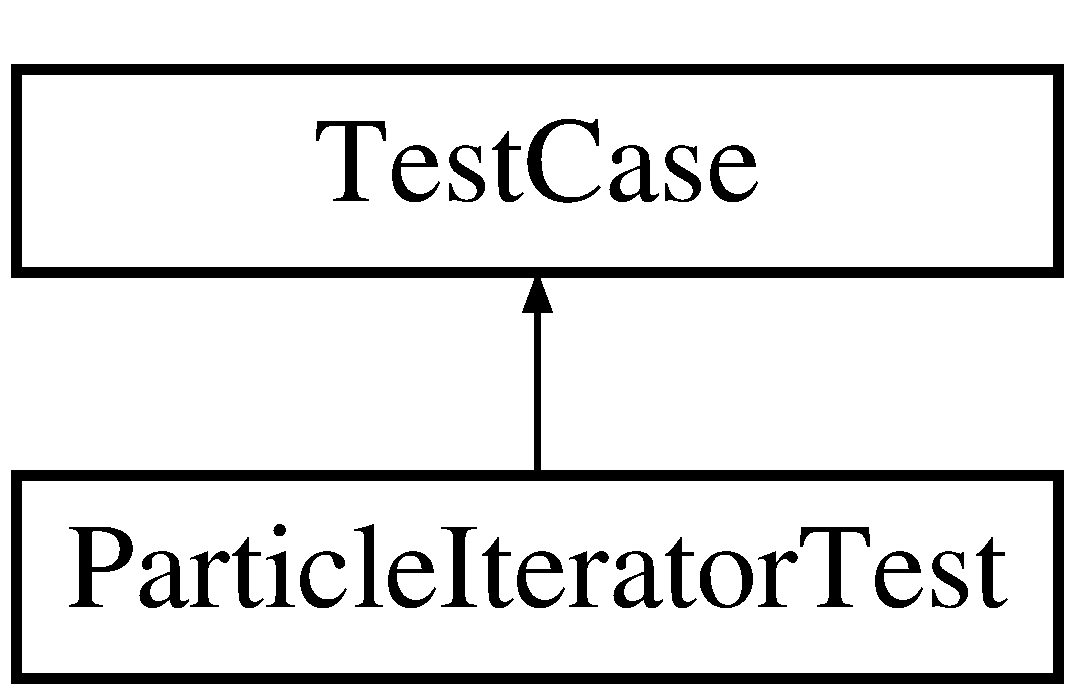
\includegraphics[height=2.000000cm]{classParticleIteratorTest}
\end{center}
\end{figure}
\subsection*{Public Member Functions}
\begin{DoxyCompactItemize}
\item 
\hyperlink{classParticleIteratorTest_a1dde0a3d917f05b50841ed9d8ea6479d}{Particle\-Iterator\-Test} ()
\item 
virtual \hyperlink{classParticleIteratorTest_acab8f6518b3738e5231fe3eb9fe4a6c3}{$\sim$\-Particle\-Iterator\-Test} ()
\item 
void \hyperlink{classParticleIteratorTest_a3955a83f802919828aa0f53f183ff0b2}{set\-Up} ()
\item 
void \hyperlink{classParticleIteratorTest_a75058ac8ad24eed571ece762eb28c5f1}{tear\-Down} ()
\item 
void \hyperlink{classParticleIteratorTest_a225ec758495ff84c6f0544744d354d56}{test\-Constructor} ()
\item 
void \hyperlink{classParticleIteratorTest_a1c35f2e945298d7767abdfa2ef888f73}{test\-Inequality} ()
\item 
void \hyperlink{classParticleIteratorTest_a6e0546482dce24998d296af47dfd07c1}{test\-Particle\-Reference} ()
\item 
void \hyperlink{classParticleIteratorTest_a115463e0363bbd4211bcc33b534e4373}{test\-Iteration} ()
\end{DoxyCompactItemize}
\subsection*{Static Public Member Functions}
\begin{DoxyCompactItemize}
\item 
static Test $\ast$ \hyperlink{classParticleIteratorTest_a75a4eb66d14bff69b51ccc4f9639c666}{suite} ()
\end{DoxyCompactItemize}
\subsection*{Private Attributes}
\begin{DoxyCompactItemize}
\item 
\hyperlink{classutils_1_1ParticleContainer}{utils\-::\-Particle\-Container} \hyperlink{classParticleIteratorTest_aed0486f4f7d7eb1cb9d0e156fc5d21c0}{container}
\item 
\hyperlink{classutils_1_1ParticleIterator}{utils\-::\-Particle\-Iterator} \hyperlink{classParticleIteratorTest_a2a0c516ec5ead4037c6eb5f0de0816cc}{particle1}
\item 
\hyperlink{classutils_1_1ParticleIterator}{utils\-::\-Particle\-Iterator} \hyperlink{classParticleIteratorTest_afb92dd60b1496e393a3c11563c4d59be}{particle2}
\item 
\hyperlink{classutils_1_1ParticleIterator}{utils\-::\-Particle\-Iterator} \hyperlink{classParticleIteratorTest_ae8a159171f6e6825c4eacd2a31b0d291}{particle3}
\end{DoxyCompactItemize}


\subsection{Constructor \& Destructor Documentation}
\hypertarget{classParticleIteratorTest_a1dde0a3d917f05b50841ed9d8ea6479d}{\index{Particle\-Iterator\-Test@{Particle\-Iterator\-Test}!Particle\-Iterator\-Test@{Particle\-Iterator\-Test}}
\index{Particle\-Iterator\-Test@{Particle\-Iterator\-Test}!ParticleIteratorTest@{Particle\-Iterator\-Test}}
\subsubsection[{Particle\-Iterator\-Test}]{\setlength{\rightskip}{0pt plus 5cm}Particle\-Iterator\-Test\-::\-Particle\-Iterator\-Test (
\begin{DoxyParamCaption}
{}
\end{DoxyParamCaption}
)}}\label{classParticleIteratorTest_a1dde0a3d917f05b50841ed9d8ea6479d}
\hypertarget{classParticleIteratorTest_acab8f6518b3738e5231fe3eb9fe4a6c3}{\index{Particle\-Iterator\-Test@{Particle\-Iterator\-Test}!$\sim$\-Particle\-Iterator\-Test@{$\sim$\-Particle\-Iterator\-Test}}
\index{$\sim$\-Particle\-Iterator\-Test@{$\sim$\-Particle\-Iterator\-Test}!ParticleIteratorTest@{Particle\-Iterator\-Test}}
\subsubsection[{$\sim$\-Particle\-Iterator\-Test}]{\setlength{\rightskip}{0pt plus 5cm}Particle\-Iterator\-Test\-::$\sim$\-Particle\-Iterator\-Test (
\begin{DoxyParamCaption}
{}
\end{DoxyParamCaption}
)\hspace{0.3cm}{\ttfamily [virtual]}}}\label{classParticleIteratorTest_acab8f6518b3738e5231fe3eb9fe4a6c3}


\subsection{Member Function Documentation}
\hypertarget{classParticleIteratorTest_a3955a83f802919828aa0f53f183ff0b2}{\index{Particle\-Iterator\-Test@{Particle\-Iterator\-Test}!set\-Up@{set\-Up}}
\index{set\-Up@{set\-Up}!ParticleIteratorTest@{Particle\-Iterator\-Test}}
\subsubsection[{set\-Up}]{\setlength{\rightskip}{0pt plus 5cm}void Particle\-Iterator\-Test\-::set\-Up (
\begin{DoxyParamCaption}
{}
\end{DoxyParamCaption}
)}}\label{classParticleIteratorTest_a3955a83f802919828aa0f53f183ff0b2}
process\-: Set up the test variables \hypertarget{classParticleIteratorTest_a75a4eb66d14bff69b51ccc4f9639c666}{\index{Particle\-Iterator\-Test@{Particle\-Iterator\-Test}!suite@{suite}}
\index{suite@{suite}!ParticleIteratorTest@{Particle\-Iterator\-Test}}
\subsubsection[{suite}]{\setlength{\rightskip}{0pt plus 5cm}Cpp\-Unit\-::\-Test $\ast$ Particle\-Iterator\-Test\-::suite (
\begin{DoxyParamCaption}
{}
\end{DoxyParamCaption}
)\hspace{0.3cm}{\ttfamily [static]}}}\label{classParticleIteratorTest_a75a4eb66d14bff69b51ccc4f9639c666}
\begin{DoxyReturn}{Returns}
the Test\-Suite for the tested methods of Particle\-Iterator 
\end{DoxyReturn}
\hypertarget{classParticleIteratorTest_a75058ac8ad24eed571ece762eb28c5f1}{\index{Particle\-Iterator\-Test@{Particle\-Iterator\-Test}!tear\-Down@{tear\-Down}}
\index{tear\-Down@{tear\-Down}!ParticleIteratorTest@{Particle\-Iterator\-Test}}
\subsubsection[{tear\-Down}]{\setlength{\rightskip}{0pt plus 5cm}void Particle\-Iterator\-Test\-::tear\-Down (
\begin{DoxyParamCaption}
{}
\end{DoxyParamCaption}
)}}\label{classParticleIteratorTest_a75058ac8ad24eed571ece762eb28c5f1}
Delete the variables \hypertarget{classParticleIteratorTest_a225ec758495ff84c6f0544744d354d56}{\index{Particle\-Iterator\-Test@{Particle\-Iterator\-Test}!test\-Constructor@{test\-Constructor}}
\index{test\-Constructor@{test\-Constructor}!ParticleIteratorTest@{Particle\-Iterator\-Test}}
\subsubsection[{test\-Constructor}]{\setlength{\rightskip}{0pt plus 5cm}void Particle\-Iterator\-Test\-::test\-Constructor (
\begin{DoxyParamCaption}
{}
\end{DoxyParamCaption}
)}}\label{classParticleIteratorTest_a225ec758495ff84c6f0544744d354d56}
Check the Constructor of the Iterator \hypertarget{classParticleIteratorTest_a1c35f2e945298d7767abdfa2ef888f73}{\index{Particle\-Iterator\-Test@{Particle\-Iterator\-Test}!test\-Inequality@{test\-Inequality}}
\index{test\-Inequality@{test\-Inequality}!ParticleIteratorTest@{Particle\-Iterator\-Test}}
\subsubsection[{test\-Inequality}]{\setlength{\rightskip}{0pt plus 5cm}void Particle\-Iterator\-Test\-::test\-Inequality (
\begin{DoxyParamCaption}
{}
\end{DoxyParamCaption}
)}}\label{classParticleIteratorTest_a1c35f2e945298d7767abdfa2ef888f73}
Check the \char`\"{}!=\char`\"{} operator of the iterator \hypertarget{classParticleIteratorTest_a115463e0363bbd4211bcc33b534e4373}{\index{Particle\-Iterator\-Test@{Particle\-Iterator\-Test}!test\-Iteration@{test\-Iteration}}
\index{test\-Iteration@{test\-Iteration}!ParticleIteratorTest@{Particle\-Iterator\-Test}}
\subsubsection[{test\-Iteration}]{\setlength{\rightskip}{0pt plus 5cm}void Particle\-Iterator\-Test\-::test\-Iteration (
\begin{DoxyParamCaption}
{}
\end{DoxyParamCaption}
)}}\label{classParticleIteratorTest_a115463e0363bbd4211bcc33b534e4373}
Check the \char`\"{}++\char`\"{} operator of the iterator \hypertarget{classParticleIteratorTest_a6e0546482dce24998d296af47dfd07c1}{\index{Particle\-Iterator\-Test@{Particle\-Iterator\-Test}!test\-Particle\-Reference@{test\-Particle\-Reference}}
\index{test\-Particle\-Reference@{test\-Particle\-Reference}!ParticleIteratorTest@{Particle\-Iterator\-Test}}
\subsubsection[{test\-Particle\-Reference}]{\setlength{\rightskip}{0pt plus 5cm}void Particle\-Iterator\-Test\-::test\-Particle\-Reference (
\begin{DoxyParamCaption}
{}
\end{DoxyParamCaption}
)}}\label{classParticleIteratorTest_a6e0546482dce24998d296af47dfd07c1}
Check the \char`\"{}$\ast$\char`\"{} operator of the iterator 

\subsection{Member Data Documentation}
\hypertarget{classParticleIteratorTest_aed0486f4f7d7eb1cb9d0e156fc5d21c0}{\index{Particle\-Iterator\-Test@{Particle\-Iterator\-Test}!container@{container}}
\index{container@{container}!ParticleIteratorTest@{Particle\-Iterator\-Test}}
\subsubsection[{container}]{\setlength{\rightskip}{0pt plus 5cm}{\bf utils\-::\-Particle\-Container} Particle\-Iterator\-Test\-::container\hspace{0.3cm}{\ttfamily [private]}}}\label{classParticleIteratorTest_aed0486f4f7d7eb1cb9d0e156fc5d21c0}
Used Container to Check the Iterator \hypertarget{classParticleIteratorTest_a2a0c516ec5ead4037c6eb5f0de0816cc}{\index{Particle\-Iterator\-Test@{Particle\-Iterator\-Test}!particle1@{particle1}}
\index{particle1@{particle1}!ParticleIteratorTest@{Particle\-Iterator\-Test}}
\subsubsection[{particle1}]{\setlength{\rightskip}{0pt plus 5cm}{\bf utils\-::\-Particle\-Iterator} Particle\-Iterator\-Test\-::particle1\hspace{0.3cm}{\ttfamily [private]}}}\label{classParticleIteratorTest_a2a0c516ec5ead4037c6eb5f0de0816cc}
Used Iterators \hypertarget{classParticleIteratorTest_afb92dd60b1496e393a3c11563c4d59be}{\index{Particle\-Iterator\-Test@{Particle\-Iterator\-Test}!particle2@{particle2}}
\index{particle2@{particle2}!ParticleIteratorTest@{Particle\-Iterator\-Test}}
\subsubsection[{particle2}]{\setlength{\rightskip}{0pt plus 5cm}{\bf utils\-::\-Particle\-Iterator} Particle\-Iterator\-Test\-::particle2\hspace{0.3cm}{\ttfamily [private]}}}\label{classParticleIteratorTest_afb92dd60b1496e393a3c11563c4d59be}
\hypertarget{classParticleIteratorTest_ae8a159171f6e6825c4eacd2a31b0d291}{\index{Particle\-Iterator\-Test@{Particle\-Iterator\-Test}!particle3@{particle3}}
\index{particle3@{particle3}!ParticleIteratorTest@{Particle\-Iterator\-Test}}
\subsubsection[{particle3}]{\setlength{\rightskip}{0pt plus 5cm}{\bf utils\-::\-Particle\-Iterator} Particle\-Iterator\-Test\-::particle3\hspace{0.3cm}{\ttfamily [private]}}}\label{classParticleIteratorTest_ae8a159171f6e6825c4eacd2a31b0d291}


The documentation for this class was generated from the following files\-:\begin{DoxyCompactItemize}
\item 
src/tests/\hyperlink{ParticleIteratorTest_8h}{Particle\-Iterator\-Test.\-h}\item 
src/tests/\hyperlink{ParticleIteratorTest_8cpp}{Particle\-Iterator\-Test.\-cpp}\end{DoxyCompactItemize}

\hypertarget{classparticles__t}{\section{particles\-\_\-t Class Reference}
\label{classparticles__t}\index{particles\-\_\-t@{particles\-\_\-t}}
}


{\ttfamily \#include $<$Input\-Particles.\-h$>$}

Inheritance diagram for particles\-\_\-t\-:\begin{figure}[H]
\begin{center}
\leavevmode
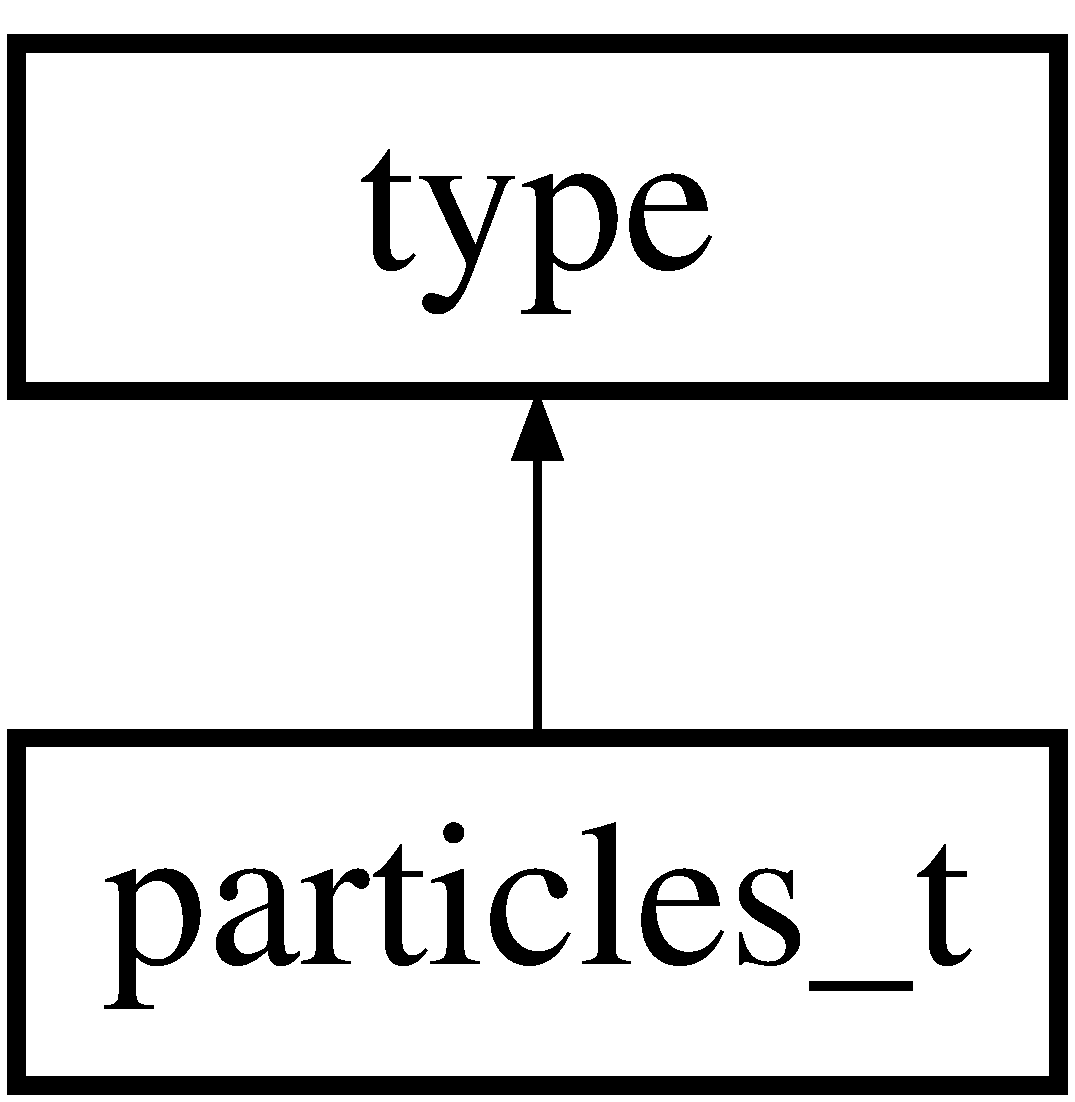
\includegraphics[height=2.000000cm]{classparticles__t}
\end{center}
\end{figure}
\subsection*{Public Types}
\begin{DoxyCompactItemize}
\item 
typedef \-::\hyperlink{classparticle__t}{particle\-\_\-t} \hyperlink{classparticles__t_af3204fae99711ad2c2e8fc73334219ef}{particle\-\_\-type}
\item 
typedef \\*
\-::xsd\-::cxx\-::tree\-::sequence\\*
$<$ \hyperlink{classparticles__t_af3204fae99711ad2c2e8fc73334219ef}{particle\-\_\-type} $>$ \hyperlink{classparticles__t_a372e39e275f0ebfb91ac53eacdb4a1f2}{particle\-\_\-sequence}
\item 
typedef particle\-\_\-sequence\-::iterator \hyperlink{classparticles__t_a876677de456e8144f2b0c51172d9dc0a}{particle\-\_\-iterator}
\item 
typedef \\*
particle\-\_\-sequence\-::const\-\_\-iterator \hyperlink{classparticles__t_a2380817b2b2e9911b8c7853d8f075ad3}{particle\-\_\-const\-\_\-iterator}
\item 
typedef \\*
\-::xsd\-::cxx\-::tree\-::traits\\*
$<$ \hyperlink{classparticles__t_af3204fae99711ad2c2e8fc73334219ef}{particle\-\_\-type}, char $>$ \hyperlink{classparticles__t_adf7984716150a259981b7f262344ee9a}{particle\-\_\-traits}
\end{DoxyCompactItemize}
\subsection*{Public Member Functions}
\begin{DoxyCompactItemize}
\item 
const \hyperlink{classparticles__t_a372e39e275f0ebfb91ac53eacdb4a1f2}{particle\-\_\-sequence} \& \hyperlink{classparticles__t_a009d0b10466f40908ac7c04372e4f23a}{particle} () const 
\item 
\hyperlink{classparticles__t_a372e39e275f0ebfb91ac53eacdb4a1f2}{particle\-\_\-sequence} \& \hyperlink{classparticles__t_a650f19bfd27cd9147cb2b0582082b1e8}{particle} ()
\item 
void \hyperlink{classparticles__t_a0cb8ecabf9a6f69ccd5fff1aed7df628}{particle} (const \hyperlink{classparticles__t_a372e39e275f0ebfb91ac53eacdb4a1f2}{particle\-\_\-sequence} \&s)
\item 
\hyperlink{classparticles__t_a9c7dcbcc9095cbb3af000a21428857e1}{particles\-\_\-t} ()
\item 
\hyperlink{classparticles__t_a9ef428228cfde19bce256f8a1f049218}{particles\-\_\-t} (const \-::xercesc\-::\-D\-O\-M\-Element \&e,\-::\hyperlink{namespacexml__schema_a0612287d030cb2732d31a45b258fdc87}{xml\-\_\-schema\-::flags} f=0,\-::\hyperlink{namespacexml__schema_ada9aa30dc722e93ee2ed7243085402a5}{xml\-\_\-schema\-::container} $\ast$c=0)
\item 
\hyperlink{classparticles__t_a514a3402a2a2b51545a1b40f1308e561}{particles\-\_\-t} (const \hyperlink{classparticles__t}{particles\-\_\-t} \&x,\-::\hyperlink{namespacexml__schema_a0612287d030cb2732d31a45b258fdc87}{xml\-\_\-schema\-::flags} f=0,\-::\hyperlink{namespacexml__schema_ada9aa30dc722e93ee2ed7243085402a5}{xml\-\_\-schema\-::container} $\ast$c=0)
\item 
virtual \hyperlink{classparticles__t}{particles\-\_\-t} $\ast$ \hyperlink{classparticles__t_a146af23d709a1d8ca6bf11b11a386850}{\-\_\-clone} (\-::\hyperlink{namespacexml__schema_a0612287d030cb2732d31a45b258fdc87}{xml\-\_\-schema\-::flags} f=0,\-::\hyperlink{namespacexml__schema_ada9aa30dc722e93ee2ed7243085402a5}{xml\-\_\-schema\-::container} $\ast$c=0) const 
\item 
virtual \hyperlink{classparticles__t_ab9b0649923ec8e2bf1cfa800560d39e4}{$\sim$particles\-\_\-t} ()
\end{DoxyCompactItemize}
\subsection*{Protected Member Functions}
\begin{DoxyCompactItemize}
\item 
void \hyperlink{classparticles__t_addce04b09439b1685fd5f09362484546}{parse} (\-::xsd\-::cxx\-::xml\-::dom\-::parser$<$ char $>$ \&,\-::\hyperlink{namespacexml__schema_a0612287d030cb2732d31a45b258fdc87}{xml\-\_\-schema\-::flags})
\end{DoxyCompactItemize}
\subsection*{Protected Attributes}
\begin{DoxyCompactItemize}
\item 
\hyperlink{classparticles__t_a372e39e275f0ebfb91ac53eacdb4a1f2}{particle\-\_\-sequence} \hyperlink{classparticles__t_adc4cfda5d19d40146fb9a640236ff2ef}{particle\-\_\-}
\end{DoxyCompactItemize}


\subsection{Member Typedef Documentation}
\hypertarget{classparticles__t_a2380817b2b2e9911b8c7853d8f075ad3}{\index{particles\-\_\-t@{particles\-\_\-t}!particle\-\_\-const\-\_\-iterator@{particle\-\_\-const\-\_\-iterator}}
\index{particle\-\_\-const\-\_\-iterator@{particle\-\_\-const\-\_\-iterator}!particles_t@{particles\-\_\-t}}
\subsubsection[{particle\-\_\-const\-\_\-iterator}]{\setlength{\rightskip}{0pt plus 5cm}typedef particle\-\_\-sequence\-::const\-\_\-iterator {\bf particles\-\_\-t\-::particle\-\_\-const\-\_\-iterator}}}\label{classparticles__t_a2380817b2b2e9911b8c7853d8f075ad3}
\hypertarget{classparticles__t_a876677de456e8144f2b0c51172d9dc0a}{\index{particles\-\_\-t@{particles\-\_\-t}!particle\-\_\-iterator@{particle\-\_\-iterator}}
\index{particle\-\_\-iterator@{particle\-\_\-iterator}!particles_t@{particles\-\_\-t}}
\subsubsection[{particle\-\_\-iterator}]{\setlength{\rightskip}{0pt plus 5cm}typedef particle\-\_\-sequence\-::iterator {\bf particles\-\_\-t\-::particle\-\_\-iterator}}}\label{classparticles__t_a876677de456e8144f2b0c51172d9dc0a}
\hypertarget{classparticles__t_a372e39e275f0ebfb91ac53eacdb4a1f2}{\index{particles\-\_\-t@{particles\-\_\-t}!particle\-\_\-sequence@{particle\-\_\-sequence}}
\index{particle\-\_\-sequence@{particle\-\_\-sequence}!particles_t@{particles\-\_\-t}}
\subsubsection[{particle\-\_\-sequence}]{\setlength{\rightskip}{0pt plus 5cm}typedef \-::xsd\-::cxx\-::tree\-::sequence$<$ {\bf particle\-\_\-type} $>$ {\bf particles\-\_\-t\-::particle\-\_\-sequence}}}\label{classparticles__t_a372e39e275f0ebfb91ac53eacdb4a1f2}
\hypertarget{classparticles__t_adf7984716150a259981b7f262344ee9a}{\index{particles\-\_\-t@{particles\-\_\-t}!particle\-\_\-traits@{particle\-\_\-traits}}
\index{particle\-\_\-traits@{particle\-\_\-traits}!particles_t@{particles\-\_\-t}}
\subsubsection[{particle\-\_\-traits}]{\setlength{\rightskip}{0pt plus 5cm}typedef \-::xsd\-::cxx\-::tree\-::traits$<$ {\bf particle\-\_\-type}, char $>$ {\bf particles\-\_\-t\-::particle\-\_\-traits}}}\label{classparticles__t_adf7984716150a259981b7f262344ee9a}
\hypertarget{classparticles__t_af3204fae99711ad2c2e8fc73334219ef}{\index{particles\-\_\-t@{particles\-\_\-t}!particle\-\_\-type@{particle\-\_\-type}}
\index{particle\-\_\-type@{particle\-\_\-type}!particles_t@{particles\-\_\-t}}
\subsubsection[{particle\-\_\-type}]{\setlength{\rightskip}{0pt plus 5cm}typedef \-::{\bf particle\-\_\-t} {\bf particles\-\_\-t\-::particle\-\_\-type}}}\label{classparticles__t_af3204fae99711ad2c2e8fc73334219ef}


\subsection{Constructor \& Destructor Documentation}
\hypertarget{classparticles__t_a9c7dcbcc9095cbb3af000a21428857e1}{\index{particles\-\_\-t@{particles\-\_\-t}!particles\-\_\-t@{particles\-\_\-t}}
\index{particles\-\_\-t@{particles\-\_\-t}!particles_t@{particles\-\_\-t}}
\subsubsection[{particles\-\_\-t}]{\setlength{\rightskip}{0pt plus 5cm}particles\-\_\-t\-::particles\-\_\-t (
\begin{DoxyParamCaption}
{}
\end{DoxyParamCaption}
)}}\label{classparticles__t_a9c7dcbcc9095cbb3af000a21428857e1}
\hypertarget{classparticles__t_a9ef428228cfde19bce256f8a1f049218}{\index{particles\-\_\-t@{particles\-\_\-t}!particles\-\_\-t@{particles\-\_\-t}}
\index{particles\-\_\-t@{particles\-\_\-t}!particles_t@{particles\-\_\-t}}
\subsubsection[{particles\-\_\-t}]{\setlength{\rightskip}{0pt plus 5cm}particles\-\_\-t\-::particles\-\_\-t (
\begin{DoxyParamCaption}
\item[{const \-::xercesc\-::\-D\-O\-M\-Element \&}]{e, }
\item[{\-::{\bf xml\-\_\-schema\-::flags}}]{f = {\ttfamily 0}, }
\item[{\-::{\bf xml\-\_\-schema\-::container} $\ast$}]{c = {\ttfamily 0}}
\end{DoxyParamCaption}
)}}\label{classparticles__t_a9ef428228cfde19bce256f8a1f049218}
\hypertarget{classparticles__t_a514a3402a2a2b51545a1b40f1308e561}{\index{particles\-\_\-t@{particles\-\_\-t}!particles\-\_\-t@{particles\-\_\-t}}
\index{particles\-\_\-t@{particles\-\_\-t}!particles_t@{particles\-\_\-t}}
\subsubsection[{particles\-\_\-t}]{\setlength{\rightskip}{0pt plus 5cm}particles\-\_\-t\-::particles\-\_\-t (
\begin{DoxyParamCaption}
\item[{const {\bf particles\-\_\-t} \&}]{x, }
\item[{\-::{\bf xml\-\_\-schema\-::flags}}]{f = {\ttfamily 0}, }
\item[{\-::{\bf xml\-\_\-schema\-::container} $\ast$}]{c = {\ttfamily 0}}
\end{DoxyParamCaption}
)}}\label{classparticles__t_a514a3402a2a2b51545a1b40f1308e561}
\hypertarget{classparticles__t_ab9b0649923ec8e2bf1cfa800560d39e4}{\index{particles\-\_\-t@{particles\-\_\-t}!$\sim$particles\-\_\-t@{$\sim$particles\-\_\-t}}
\index{$\sim$particles\-\_\-t@{$\sim$particles\-\_\-t}!particles_t@{particles\-\_\-t}}
\subsubsection[{$\sim$particles\-\_\-t}]{\setlength{\rightskip}{0pt plus 5cm}particles\-\_\-t\-::$\sim$particles\-\_\-t (
\begin{DoxyParamCaption}
{}
\end{DoxyParamCaption}
)\hspace{0.3cm}{\ttfamily [virtual]}}}\label{classparticles__t_ab9b0649923ec8e2bf1cfa800560d39e4}


\subsection{Member Function Documentation}
\hypertarget{classparticles__t_a146af23d709a1d8ca6bf11b11a386850}{\index{particles\-\_\-t@{particles\-\_\-t}!\-\_\-clone@{\-\_\-clone}}
\index{\-\_\-clone@{\-\_\-clone}!particles_t@{particles\-\_\-t}}
\subsubsection[{\-\_\-clone}]{\setlength{\rightskip}{0pt plus 5cm}{\bf particles\-\_\-t} $\ast$ particles\-\_\-t\-::\-\_\-clone (
\begin{DoxyParamCaption}
\item[{\-::{\bf xml\-\_\-schema\-::flags}}]{f = {\ttfamily 0}, }
\item[{\-::{\bf xml\-\_\-schema\-::container} $\ast$}]{c = {\ttfamily 0}}
\end{DoxyParamCaption}
) const\hspace{0.3cm}{\ttfamily [virtual]}}}\label{classparticles__t_a146af23d709a1d8ca6bf11b11a386850}
\hypertarget{classparticles__t_addce04b09439b1685fd5f09362484546}{\index{particles\-\_\-t@{particles\-\_\-t}!parse@{parse}}
\index{parse@{parse}!particles_t@{particles\-\_\-t}}
\subsubsection[{parse}]{\setlength{\rightskip}{0pt plus 5cm}void particles\-\_\-t\-::parse (
\begin{DoxyParamCaption}
\item[{\-::xsd\-::cxx\-::xml\-::dom\-::parser$<$ char $>$ \&}]{p, }
\item[{\-::{\bf xml\-\_\-schema\-::flags}}]{f}
\end{DoxyParamCaption}
)\hspace{0.3cm}{\ttfamily [protected]}}}\label{classparticles__t_addce04b09439b1685fd5f09362484546}
\hypertarget{classparticles__t_a009d0b10466f40908ac7c04372e4f23a}{\index{particles\-\_\-t@{particles\-\_\-t}!particle@{particle}}
\index{particle@{particle}!particles_t@{particles\-\_\-t}}
\subsubsection[{particle}]{\setlength{\rightskip}{0pt plus 5cm}const {\bf particles\-\_\-t\-::particle\-\_\-sequence} \& particles\-\_\-t\-::particle (
\begin{DoxyParamCaption}
{}
\end{DoxyParamCaption}
) const}}\label{classparticles__t_a009d0b10466f40908ac7c04372e4f23a}
\hypertarget{classparticles__t_a650f19bfd27cd9147cb2b0582082b1e8}{\index{particles\-\_\-t@{particles\-\_\-t}!particle@{particle}}
\index{particle@{particle}!particles_t@{particles\-\_\-t}}
\subsubsection[{particle}]{\setlength{\rightskip}{0pt plus 5cm}{\bf particles\-\_\-t\-::particle\-\_\-sequence} \& particles\-\_\-t\-::particle (
\begin{DoxyParamCaption}
{}
\end{DoxyParamCaption}
)}}\label{classparticles__t_a650f19bfd27cd9147cb2b0582082b1e8}
\hypertarget{classparticles__t_a0cb8ecabf9a6f69ccd5fff1aed7df628}{\index{particles\-\_\-t@{particles\-\_\-t}!particle@{particle}}
\index{particle@{particle}!particles_t@{particles\-\_\-t}}
\subsubsection[{particle}]{\setlength{\rightskip}{0pt plus 5cm}void particles\-\_\-t\-::particle (
\begin{DoxyParamCaption}
\item[{const {\bf particle\-\_\-sequence} \&}]{s}
\end{DoxyParamCaption}
)}}\label{classparticles__t_a0cb8ecabf9a6f69ccd5fff1aed7df628}


\subsection{Member Data Documentation}
\hypertarget{classparticles__t_adc4cfda5d19d40146fb9a640236ff2ef}{\index{particles\-\_\-t@{particles\-\_\-t}!particle\-\_\-@{particle\-\_\-}}
\index{particle\-\_\-@{particle\-\_\-}!particles_t@{particles\-\_\-t}}
\subsubsection[{particle\-\_\-}]{\setlength{\rightskip}{0pt plus 5cm}{\bf particle\-\_\-sequence} particles\-\_\-t\-::particle\-\_\-\hspace{0.3cm}{\ttfamily [protected]}}}\label{classparticles__t_adc4cfda5d19d40146fb9a640236ff2ef}


The documentation for this class was generated from the following files\-:\begin{DoxyCompactItemize}
\item 
src/utils/\hyperlink{InputParticles_8h}{Input\-Particles.\-h}\item 
src/utils/\hyperlink{InputParticles_8cpp}{Input\-Particles.\-cpp}\end{DoxyCompactItemize}

\hypertarget{classPieceUnstructuredGrid__t}{\section{Piece\-Unstructured\-Grid\-\_\-t Class Reference}
\label{classPieceUnstructuredGrid__t}\index{Piece\-Unstructured\-Grid\-\_\-t@{Piece\-Unstructured\-Grid\-\_\-t}}
}


Class corresponding to the Piece\-Unstructured\-Grid\-\_\-t schema type.  




{\ttfamily \#include $<$vtk-\/unstructured.\-h$>$}

Inheritance diagram for Piece\-Unstructured\-Grid\-\_\-t\-:\begin{figure}[H]
\begin{center}
\leavevmode
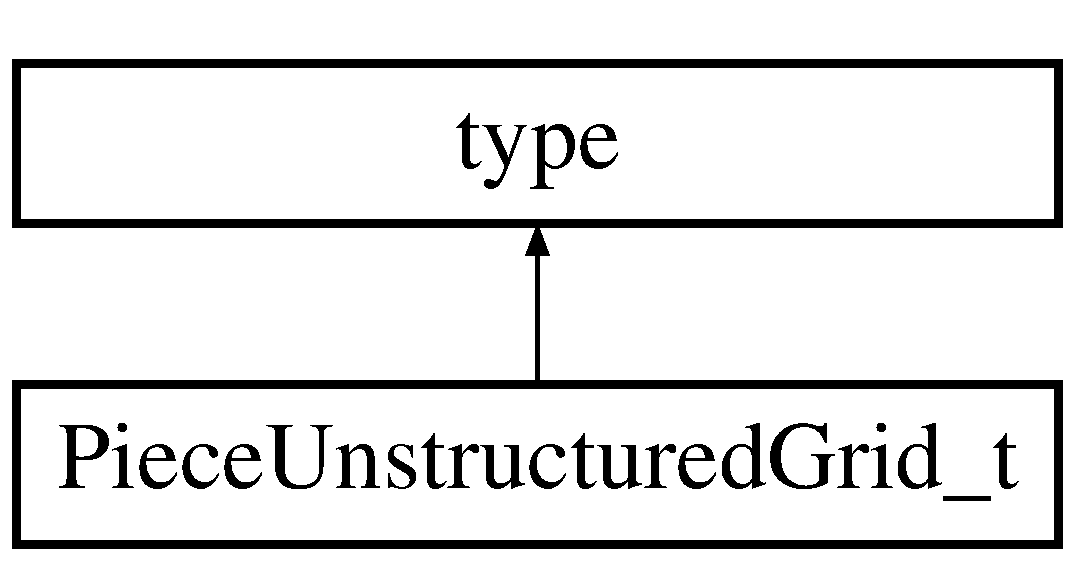
\includegraphics[height=2.000000cm]{classPieceUnstructuredGrid__t}
\end{center}
\end{figure}
\subsection*{Public Member Functions}
\begin{DoxyCompactItemize}
\item 
virtual \hyperlink{classPieceUnstructuredGrid__t_a9d1eb720775ac4e3b7778f898decc264}{$\sim$\-Piece\-Unstructured\-Grid\-\_\-t} ()
\begin{DoxyCompactList}\small\item\em Destructor. \end{DoxyCompactList}\end{DoxyCompactItemize}
\subsection*{Point\-Data}
\label{_amgrpe540450fb956cd9dbb96f979e5939d0f}%
Accessor and modifier functions for the Point\-Data required element. \begin{DoxyCompactItemize}
\item 
typedef \-::\hyperlink{classPointData}{Point\-Data} \hyperlink{classPieceUnstructuredGrid__t_a5d79d8ea03ca53f80f24e62c2175ec02}{Point\-Data\-\_\-type}
\begin{DoxyCompactList}\small\item\em Element type. \end{DoxyCompactList}\item 
typedef \\*
\-::xsd\-::cxx\-::tree\-::traits\\*
$<$ \hyperlink{classPieceUnstructuredGrid__t_a5d79d8ea03ca53f80f24e62c2175ec02}{Point\-Data\-\_\-type}, char $>$ \hyperlink{classPieceUnstructuredGrid__t_aee3c7ac7c46c4ebc9f248d31c458d300}{Point\-Data\-\_\-traits}
\begin{DoxyCompactList}\small\item\em Element traits type. \end{DoxyCompactList}\item 
const \hyperlink{classPieceUnstructuredGrid__t_a5d79d8ea03ca53f80f24e62c2175ec02}{Point\-Data\-\_\-type} \& \hyperlink{classPieceUnstructuredGrid__t_a4825627cfe05949b680c81826e9d4ea5}{Point\-Data} () const 
\begin{DoxyCompactList}\small\item\em Return a read-\/only (constant) reference to the element. \end{DoxyCompactList}\item 
\hyperlink{classPieceUnstructuredGrid__t_a5d79d8ea03ca53f80f24e62c2175ec02}{Point\-Data\-\_\-type} \& \hyperlink{classPieceUnstructuredGrid__t_af3a9955626dac2aad17bf879a77d2c0d}{Point\-Data} ()
\begin{DoxyCompactList}\small\item\em Return a read-\/write reference to the element. \end{DoxyCompactList}\item 
void \hyperlink{classPieceUnstructuredGrid__t_aee7745ad1ce39af5fc048e50acb76424}{Point\-Data} (const \hyperlink{classPieceUnstructuredGrid__t_a5d79d8ea03ca53f80f24e62c2175ec02}{Point\-Data\-\_\-type} \&x)
\begin{DoxyCompactList}\small\item\em Set the element value. \end{DoxyCompactList}\item 
void \hyperlink{classPieceUnstructuredGrid__t_a752f5abf0faba70deaab0b4990677612}{Point\-Data} (\-::std\-::auto\-\_\-ptr$<$ \hyperlink{classPieceUnstructuredGrid__t_a5d79d8ea03ca53f80f24e62c2175ec02}{Point\-Data\-\_\-type} $>$ p)
\begin{DoxyCompactList}\small\item\em Set the element value without copying. \end{DoxyCompactList}\end{DoxyCompactItemize}
\subsection*{Cell\-Data}
\label{_amgrp007b3d9997e1a909fe32a9f90c4a9977}%
Accessor and modifier functions for the Cell\-Data required element. \begin{DoxyCompactItemize}
\item 
typedef \-::\hyperlink{classCellData}{Cell\-Data} \hyperlink{classPieceUnstructuredGrid__t_a4232a7b88477ee6f692a4e5fab6a65d1}{Cell\-Data\-\_\-type}
\begin{DoxyCompactList}\small\item\em Element type. \end{DoxyCompactList}\item 
typedef \\*
\-::xsd\-::cxx\-::tree\-::traits\\*
$<$ \hyperlink{classPieceUnstructuredGrid__t_a4232a7b88477ee6f692a4e5fab6a65d1}{Cell\-Data\-\_\-type}, char $>$ \hyperlink{classPieceUnstructuredGrid__t_a0e04d369c16993da7e5e2a7152c2e518}{Cell\-Data\-\_\-traits}
\begin{DoxyCompactList}\small\item\em Element traits type. \end{DoxyCompactList}\item 
const \hyperlink{classPieceUnstructuredGrid__t_a4232a7b88477ee6f692a4e5fab6a65d1}{Cell\-Data\-\_\-type} \& \hyperlink{classPieceUnstructuredGrid__t_a7c7be2b175fa0ec2fc403bb4740865c1}{Cell\-Data} () const 
\begin{DoxyCompactList}\small\item\em Return a read-\/only (constant) reference to the element. \end{DoxyCompactList}\item 
\hyperlink{classPieceUnstructuredGrid__t_a4232a7b88477ee6f692a4e5fab6a65d1}{Cell\-Data\-\_\-type} \& \hyperlink{classPieceUnstructuredGrid__t_a679db045d830876cce6fe04767e7c611}{Cell\-Data} ()
\begin{DoxyCompactList}\small\item\em Return a read-\/write reference to the element. \end{DoxyCompactList}\item 
void \hyperlink{classPieceUnstructuredGrid__t_a6fd0984f28544ef312e860cac18e7144}{Cell\-Data} (const \hyperlink{classPieceUnstructuredGrid__t_a4232a7b88477ee6f692a4e5fab6a65d1}{Cell\-Data\-\_\-type} \&x)
\begin{DoxyCompactList}\small\item\em Set the element value. \end{DoxyCompactList}\item 
void \hyperlink{classPieceUnstructuredGrid__t_af669b0f503d52e5edc2cc0665dc64721}{Cell\-Data} (\-::std\-::auto\-\_\-ptr$<$ \hyperlink{classPieceUnstructuredGrid__t_a4232a7b88477ee6f692a4e5fab6a65d1}{Cell\-Data\-\_\-type} $>$ p)
\begin{DoxyCompactList}\small\item\em Set the element value without copying. \end{DoxyCompactList}\end{DoxyCompactItemize}
\subsection*{Points}
\label{_amgrp75dd5f1160a3f02b6fae89c54361a1b3}%
Accessor and modifier functions for the Points required element. \begin{DoxyCompactItemize}
\item 
typedef \-::\hyperlink{classPoints}{Points} \hyperlink{classPieceUnstructuredGrid__t_a7747b159a3d1eee8d02a0eefaa235711}{Points\-\_\-type}
\begin{DoxyCompactList}\small\item\em Element type. \end{DoxyCompactList}\item 
typedef \\*
\-::xsd\-::cxx\-::tree\-::traits\\*
$<$ \hyperlink{classPieceUnstructuredGrid__t_a7747b159a3d1eee8d02a0eefaa235711}{Points\-\_\-type}, char $>$ \hyperlink{classPieceUnstructuredGrid__t_abdfd9c9f9eb5f43bd4cfcb2fad6d9f63}{Points\-\_\-traits}
\begin{DoxyCompactList}\small\item\em Element traits type. \end{DoxyCompactList}\item 
const \hyperlink{classPieceUnstructuredGrid__t_a7747b159a3d1eee8d02a0eefaa235711}{Points\-\_\-type} \& \hyperlink{classPieceUnstructuredGrid__t_a53dfd670cb335d13003dc229343a0fa1}{Points} () const 
\begin{DoxyCompactList}\small\item\em Return a read-\/only (constant) reference to the element. \end{DoxyCompactList}\item 
\hyperlink{classPieceUnstructuredGrid__t_a7747b159a3d1eee8d02a0eefaa235711}{Points\-\_\-type} \& \hyperlink{classPieceUnstructuredGrid__t_aa8e21b391979e8e2e22361e3b29e0276}{Points} ()
\begin{DoxyCompactList}\small\item\em Return a read-\/write reference to the element. \end{DoxyCompactList}\item 
void \hyperlink{classPieceUnstructuredGrid__t_ab653af7be8fbe0d3458bf8cd5cdf3668}{Points} (const \hyperlink{classPieceUnstructuredGrid__t_a7747b159a3d1eee8d02a0eefaa235711}{Points\-\_\-type} \&x)
\begin{DoxyCompactList}\small\item\em Set the element value. \end{DoxyCompactList}\item 
void \hyperlink{classPieceUnstructuredGrid__t_a3a44ef2850c664e89d79075a51497b17}{Points} (\-::std\-::auto\-\_\-ptr$<$ \hyperlink{classPieceUnstructuredGrid__t_a7747b159a3d1eee8d02a0eefaa235711}{Points\-\_\-type} $>$ p)
\begin{DoxyCompactList}\small\item\em Set the element value without copying. \end{DoxyCompactList}\end{DoxyCompactItemize}
\subsection*{Cells}
\label{_amgrp56284b76007b9f31cdec47174c4de6af}%
Accessor and modifier functions for the Cells required element. \begin{DoxyCompactItemize}
\item 
typedef \-::\hyperlink{classCells}{Cells} \hyperlink{classPieceUnstructuredGrid__t_aca1ec38eff08bde0cd115c54dbb7a20f}{Cells\-\_\-type}
\begin{DoxyCompactList}\small\item\em Element type. \end{DoxyCompactList}\item 
typedef \\*
\-::xsd\-::cxx\-::tree\-::traits\\*
$<$ \hyperlink{classPieceUnstructuredGrid__t_aca1ec38eff08bde0cd115c54dbb7a20f}{Cells\-\_\-type}, char $>$ \hyperlink{classPieceUnstructuredGrid__t_a33252b6f55b5ae830ceecdf9be42cce1}{Cells\-\_\-traits}
\begin{DoxyCompactList}\small\item\em Element traits type. \end{DoxyCompactList}\item 
const \hyperlink{classPieceUnstructuredGrid__t_aca1ec38eff08bde0cd115c54dbb7a20f}{Cells\-\_\-type} \& \hyperlink{classPieceUnstructuredGrid__t_a398de7c2f319c1785810e18f6b43831e}{Cells} () const 
\begin{DoxyCompactList}\small\item\em Return a read-\/only (constant) reference to the element. \end{DoxyCompactList}\item 
\hyperlink{classPieceUnstructuredGrid__t_aca1ec38eff08bde0cd115c54dbb7a20f}{Cells\-\_\-type} \& \hyperlink{classPieceUnstructuredGrid__t_a49e65eacff6577cd353fa15a09febf86}{Cells} ()
\begin{DoxyCompactList}\small\item\em Return a read-\/write reference to the element. \end{DoxyCompactList}\item 
void \hyperlink{classPieceUnstructuredGrid__t_a366f0cff854ef350eb1be9da22df6d14}{Cells} (const \hyperlink{classPieceUnstructuredGrid__t_aca1ec38eff08bde0cd115c54dbb7a20f}{Cells\-\_\-type} \&x)
\begin{DoxyCompactList}\small\item\em Set the element value. \end{DoxyCompactList}\item 
void \hyperlink{classPieceUnstructuredGrid__t_ab90d26fbc66b1b669b7bfa7a50a6b069}{Cells} (\-::std\-::auto\-\_\-ptr$<$ \hyperlink{classPieceUnstructuredGrid__t_aca1ec38eff08bde0cd115c54dbb7a20f}{Cells\-\_\-type} $>$ p)
\begin{DoxyCompactList}\small\item\em Set the element value without copying. \end{DoxyCompactList}\end{DoxyCompactItemize}
\subsection*{Number\-Of\-Points}
\label{_amgrp38600d7fb1ccb3e7ee12b901540b4f7d}%
Accessor and modifier functions for the Number\-Of\-Points required attribute. \begin{DoxyCompactItemize}
\item 
typedef \-::\hyperlink{namespacexml__schema_aaaea7c8ce4dfbe26cc52c91c29c97b7c}{xml\-\_\-schema\-::integer} \hyperlink{classPieceUnstructuredGrid__t_a8df1cd0d138d990e166d325ceed9a660}{Number\-Of\-Points\-\_\-type}
\begin{DoxyCompactList}\small\item\em Attribute type. \end{DoxyCompactList}\item 
typedef \\*
\-::xsd\-::cxx\-::tree\-::traits\\*
$<$ \hyperlink{classPieceUnstructuredGrid__t_a8df1cd0d138d990e166d325ceed9a660}{Number\-Of\-Points\-\_\-type}, char $>$ \hyperlink{classPieceUnstructuredGrid__t_acdfbb1dc264a5a48bcc6d4aa815db003}{Number\-Of\-Points\-\_\-traits}
\begin{DoxyCompactList}\small\item\em Attribute traits type. \end{DoxyCompactList}\item 
const \hyperlink{classPieceUnstructuredGrid__t_a8df1cd0d138d990e166d325ceed9a660}{Number\-Of\-Points\-\_\-type} \& \hyperlink{classPieceUnstructuredGrid__t_a6fe4a92f59d9a837e046bf3d51e79b33}{Number\-Of\-Points} () const 
\begin{DoxyCompactList}\small\item\em Return a read-\/only (constant) reference to the attribute. \end{DoxyCompactList}\item 
\hyperlink{classPieceUnstructuredGrid__t_a8df1cd0d138d990e166d325ceed9a660}{Number\-Of\-Points\-\_\-type} \& \hyperlink{classPieceUnstructuredGrid__t_adadae535c3c291dc01dd0be3315d9dbc}{Number\-Of\-Points} ()
\begin{DoxyCompactList}\small\item\em Return a read-\/write reference to the attribute. \end{DoxyCompactList}\item 
void \hyperlink{classPieceUnstructuredGrid__t_a3e4e5defa42f9ecebb2016ca1d207700}{Number\-Of\-Points} (const \hyperlink{classPieceUnstructuredGrid__t_a8df1cd0d138d990e166d325ceed9a660}{Number\-Of\-Points\-\_\-type} \&x)
\begin{DoxyCompactList}\small\item\em Set the attribute value. \end{DoxyCompactList}\end{DoxyCompactItemize}
\subsection*{Number\-Of\-Cells}
\label{_amgrp967ac3c5aad15a640629bb3adc1fc287}%
Accessor and modifier functions for the Number\-Of\-Cells required attribute. \begin{DoxyCompactItemize}
\item 
typedef \-::\hyperlink{namespacexml__schema_aaaea7c8ce4dfbe26cc52c91c29c97b7c}{xml\-\_\-schema\-::integer} \hyperlink{classPieceUnstructuredGrid__t_aeae5546900c50a4abe9b3aea485e97d0}{Number\-Of\-Cells\-\_\-type}
\begin{DoxyCompactList}\small\item\em Attribute type. \end{DoxyCompactList}\item 
typedef \\*
\-::xsd\-::cxx\-::tree\-::traits\\*
$<$ \hyperlink{classPieceUnstructuredGrid__t_aeae5546900c50a4abe9b3aea485e97d0}{Number\-Of\-Cells\-\_\-type}, char $>$ \hyperlink{classPieceUnstructuredGrid__t_a7c7607d306bde9e187b9cb3f570d6155}{Number\-Of\-Cells\-\_\-traits}
\begin{DoxyCompactList}\small\item\em Attribute traits type. \end{DoxyCompactList}\item 
const \hyperlink{classPieceUnstructuredGrid__t_aeae5546900c50a4abe9b3aea485e97d0}{Number\-Of\-Cells\-\_\-type} \& \hyperlink{classPieceUnstructuredGrid__t_a6e395db39208cc81f9d7093c50d5d334}{Number\-Of\-Cells} () const 
\begin{DoxyCompactList}\small\item\em Return a read-\/only (constant) reference to the attribute. \end{DoxyCompactList}\item 
\hyperlink{classPieceUnstructuredGrid__t_aeae5546900c50a4abe9b3aea485e97d0}{Number\-Of\-Cells\-\_\-type} \& \hyperlink{classPieceUnstructuredGrid__t_abe5f21a859d968d4b23a9b7ad790a7b3}{Number\-Of\-Cells} ()
\begin{DoxyCompactList}\small\item\em Return a read-\/write reference to the attribute. \end{DoxyCompactList}\item 
void \hyperlink{classPieceUnstructuredGrid__t_a25296cecd9f9c30f8c75ed8b750c1ad7}{Number\-Of\-Cells} (const \hyperlink{classPieceUnstructuredGrid__t_aeae5546900c50a4abe9b3aea485e97d0}{Number\-Of\-Cells\-\_\-type} \&x)
\begin{DoxyCompactList}\small\item\em Set the attribute value. \end{DoxyCompactList}\end{DoxyCompactItemize}
\subsection*{Constructors}
\begin{DoxyCompactItemize}
\item 
\hyperlink{classPieceUnstructuredGrid__t_a9d30b76eb9efa7565011da966d5c0df7}{Piece\-Unstructured\-Grid\-\_\-t} (const \hyperlink{classPieceUnstructuredGrid__t_a5d79d8ea03ca53f80f24e62c2175ec02}{Point\-Data\-\_\-type} \&, const \hyperlink{classPieceUnstructuredGrid__t_a4232a7b88477ee6f692a4e5fab6a65d1}{Cell\-Data\-\_\-type} \&, const \hyperlink{classPieceUnstructuredGrid__t_a7747b159a3d1eee8d02a0eefaa235711}{Points\-\_\-type} \&, const \hyperlink{classPieceUnstructuredGrid__t_aca1ec38eff08bde0cd115c54dbb7a20f}{Cells\-\_\-type} \&, const \hyperlink{classPieceUnstructuredGrid__t_a8df1cd0d138d990e166d325ceed9a660}{Number\-Of\-Points\-\_\-type} \&, const \hyperlink{classPieceUnstructuredGrid__t_aeae5546900c50a4abe9b3aea485e97d0}{Number\-Of\-Cells\-\_\-type} \&)
\begin{DoxyCompactList}\small\item\em Create an instance from the ultimate base and initializers for required elements and attributes. \end{DoxyCompactList}\item 
\hyperlink{classPieceUnstructuredGrid__t_a2b90af1916dfe3153cb1d630af5af490}{Piece\-Unstructured\-Grid\-\_\-t} (\-::std\-::auto\-\_\-ptr$<$ \hyperlink{classPieceUnstructuredGrid__t_a5d79d8ea03ca53f80f24e62c2175ec02}{Point\-Data\-\_\-type} $>$ \&,\-::std\-::auto\-\_\-ptr$<$ \hyperlink{classPieceUnstructuredGrid__t_a4232a7b88477ee6f692a4e5fab6a65d1}{Cell\-Data\-\_\-type} $>$ \&,\-::std\-::auto\-\_\-ptr$<$ \hyperlink{classPieceUnstructuredGrid__t_a7747b159a3d1eee8d02a0eefaa235711}{Points\-\_\-type} $>$ \&,\-::std\-::auto\-\_\-ptr$<$ \hyperlink{classPieceUnstructuredGrid__t_aca1ec38eff08bde0cd115c54dbb7a20f}{Cells\-\_\-type} $>$ \&, const \hyperlink{classPieceUnstructuredGrid__t_a8df1cd0d138d990e166d325ceed9a660}{Number\-Of\-Points\-\_\-type} \&, const \hyperlink{classPieceUnstructuredGrid__t_aeae5546900c50a4abe9b3aea485e97d0}{Number\-Of\-Cells\-\_\-type} \&)
\begin{DoxyCompactList}\small\item\em Create an instance from the ultimate base and initializers for required elements and attributes (auto\-\_\-ptr version). \end{DoxyCompactList}\item 
\hyperlink{classPieceUnstructuredGrid__t_a56c6d065b161aa4f28789044d082c622}{Piece\-Unstructured\-Grid\-\_\-t} (const \-::xercesc\-::\-D\-O\-M\-Element \&e,\-::\hyperlink{namespacexml__schema_a0612287d030cb2732d31a45b258fdc87}{xml\-\_\-schema\-::flags} f=0,\-::\hyperlink{namespacexml__schema_ada9aa30dc722e93ee2ed7243085402a5}{xml\-\_\-schema\-::container} $\ast$c=0)
\begin{DoxyCompactList}\small\item\em Create an instance from a D\-O\-M element. \end{DoxyCompactList}\item 
\hyperlink{classPieceUnstructuredGrid__t_a6a1c61bdda2b5458715e902eae2420f9}{Piece\-Unstructured\-Grid\-\_\-t} (const \hyperlink{classPieceUnstructuredGrid__t}{Piece\-Unstructured\-Grid\-\_\-t} \&x,\-::\hyperlink{namespacexml__schema_a0612287d030cb2732d31a45b258fdc87}{xml\-\_\-schema\-::flags} f=0,\-::\hyperlink{namespacexml__schema_ada9aa30dc722e93ee2ed7243085402a5}{xml\-\_\-schema\-::container} $\ast$c=0)
\begin{DoxyCompactList}\small\item\em Copy constructor. \end{DoxyCompactList}\item 
virtual \hyperlink{classPieceUnstructuredGrid__t}{Piece\-Unstructured\-Grid\-\_\-t} $\ast$ \hyperlink{classPieceUnstructuredGrid__t_a48f6dcab2714e3f907993e1c99bcc8b2}{\-\_\-clone} (\-::\hyperlink{namespacexml__schema_a0612287d030cb2732d31a45b258fdc87}{xml\-\_\-schema\-::flags} f=0,\-::\hyperlink{namespacexml__schema_ada9aa30dc722e93ee2ed7243085402a5}{xml\-\_\-schema\-::container} $\ast$c=0) const 
\begin{DoxyCompactList}\small\item\em Copy the instance polymorphically. \end{DoxyCompactList}\end{DoxyCompactItemize}


\subsection{Detailed Description}
Class corresponding to the Piece\-Unstructured\-Grid\-\_\-t schema type. 

\subsection{Member Typedef Documentation}
\hypertarget{classPieceUnstructuredGrid__t_a0e04d369c16993da7e5e2a7152c2e518}{\index{Piece\-Unstructured\-Grid\-\_\-t@{Piece\-Unstructured\-Grid\-\_\-t}!Cell\-Data\-\_\-traits@{Cell\-Data\-\_\-traits}}
\index{Cell\-Data\-\_\-traits@{Cell\-Data\-\_\-traits}!PieceUnstructuredGrid_t@{Piece\-Unstructured\-Grid\-\_\-t}}
\subsubsection[{Cell\-Data\-\_\-traits}]{\setlength{\rightskip}{0pt plus 5cm}typedef \-::xsd\-::cxx\-::tree\-::traits$<$ {\bf Cell\-Data\-\_\-type}, char $>$ {\bf Piece\-Unstructured\-Grid\-\_\-t\-::\-Cell\-Data\-\_\-traits}}}\label{classPieceUnstructuredGrid__t_a0e04d369c16993da7e5e2a7152c2e518}


Element traits type. 

\hypertarget{classPieceUnstructuredGrid__t_a4232a7b88477ee6f692a4e5fab6a65d1}{\index{Piece\-Unstructured\-Grid\-\_\-t@{Piece\-Unstructured\-Grid\-\_\-t}!Cell\-Data\-\_\-type@{Cell\-Data\-\_\-type}}
\index{Cell\-Data\-\_\-type@{Cell\-Data\-\_\-type}!PieceUnstructuredGrid_t@{Piece\-Unstructured\-Grid\-\_\-t}}
\subsubsection[{Cell\-Data\-\_\-type}]{\setlength{\rightskip}{0pt plus 5cm}typedef \-::{\bf Cell\-Data} {\bf Piece\-Unstructured\-Grid\-\_\-t\-::\-Cell\-Data\-\_\-type}}}\label{classPieceUnstructuredGrid__t_a4232a7b88477ee6f692a4e5fab6a65d1}


Element type. 

\hypertarget{classPieceUnstructuredGrid__t_a33252b6f55b5ae830ceecdf9be42cce1}{\index{Piece\-Unstructured\-Grid\-\_\-t@{Piece\-Unstructured\-Grid\-\_\-t}!Cells\-\_\-traits@{Cells\-\_\-traits}}
\index{Cells\-\_\-traits@{Cells\-\_\-traits}!PieceUnstructuredGrid_t@{Piece\-Unstructured\-Grid\-\_\-t}}
\subsubsection[{Cells\-\_\-traits}]{\setlength{\rightskip}{0pt plus 5cm}typedef \-::xsd\-::cxx\-::tree\-::traits$<$ {\bf Cells\-\_\-type}, char $>$ {\bf Piece\-Unstructured\-Grid\-\_\-t\-::\-Cells\-\_\-traits}}}\label{classPieceUnstructuredGrid__t_a33252b6f55b5ae830ceecdf9be42cce1}


Element traits type. 

\hypertarget{classPieceUnstructuredGrid__t_aca1ec38eff08bde0cd115c54dbb7a20f}{\index{Piece\-Unstructured\-Grid\-\_\-t@{Piece\-Unstructured\-Grid\-\_\-t}!Cells\-\_\-type@{Cells\-\_\-type}}
\index{Cells\-\_\-type@{Cells\-\_\-type}!PieceUnstructuredGrid_t@{Piece\-Unstructured\-Grid\-\_\-t}}
\subsubsection[{Cells\-\_\-type}]{\setlength{\rightskip}{0pt plus 5cm}typedef \-::{\bf Cells} {\bf Piece\-Unstructured\-Grid\-\_\-t\-::\-Cells\-\_\-type}}}\label{classPieceUnstructuredGrid__t_aca1ec38eff08bde0cd115c54dbb7a20f}


Element type. 

\hypertarget{classPieceUnstructuredGrid__t_a7c7607d306bde9e187b9cb3f570d6155}{\index{Piece\-Unstructured\-Grid\-\_\-t@{Piece\-Unstructured\-Grid\-\_\-t}!Number\-Of\-Cells\-\_\-traits@{Number\-Of\-Cells\-\_\-traits}}
\index{Number\-Of\-Cells\-\_\-traits@{Number\-Of\-Cells\-\_\-traits}!PieceUnstructuredGrid_t@{Piece\-Unstructured\-Grid\-\_\-t}}
\subsubsection[{Number\-Of\-Cells\-\_\-traits}]{\setlength{\rightskip}{0pt plus 5cm}typedef \-::xsd\-::cxx\-::tree\-::traits$<$ {\bf Number\-Of\-Cells\-\_\-type}, char $>$ {\bf Piece\-Unstructured\-Grid\-\_\-t\-::\-Number\-Of\-Cells\-\_\-traits}}}\label{classPieceUnstructuredGrid__t_a7c7607d306bde9e187b9cb3f570d6155}


Attribute traits type. 

\hypertarget{classPieceUnstructuredGrid__t_aeae5546900c50a4abe9b3aea485e97d0}{\index{Piece\-Unstructured\-Grid\-\_\-t@{Piece\-Unstructured\-Grid\-\_\-t}!Number\-Of\-Cells\-\_\-type@{Number\-Of\-Cells\-\_\-type}}
\index{Number\-Of\-Cells\-\_\-type@{Number\-Of\-Cells\-\_\-type}!PieceUnstructuredGrid_t@{Piece\-Unstructured\-Grid\-\_\-t}}
\subsubsection[{Number\-Of\-Cells\-\_\-type}]{\setlength{\rightskip}{0pt plus 5cm}typedef \-::{\bf xml\-\_\-schema\-::integer} {\bf Piece\-Unstructured\-Grid\-\_\-t\-::\-Number\-Of\-Cells\-\_\-type}}}\label{classPieceUnstructuredGrid__t_aeae5546900c50a4abe9b3aea485e97d0}


Attribute type. 

\hypertarget{classPieceUnstructuredGrid__t_acdfbb1dc264a5a48bcc6d4aa815db003}{\index{Piece\-Unstructured\-Grid\-\_\-t@{Piece\-Unstructured\-Grid\-\_\-t}!Number\-Of\-Points\-\_\-traits@{Number\-Of\-Points\-\_\-traits}}
\index{Number\-Of\-Points\-\_\-traits@{Number\-Of\-Points\-\_\-traits}!PieceUnstructuredGrid_t@{Piece\-Unstructured\-Grid\-\_\-t}}
\subsubsection[{Number\-Of\-Points\-\_\-traits}]{\setlength{\rightskip}{0pt plus 5cm}typedef \-::xsd\-::cxx\-::tree\-::traits$<$ {\bf Number\-Of\-Points\-\_\-type}, char $>$ {\bf Piece\-Unstructured\-Grid\-\_\-t\-::\-Number\-Of\-Points\-\_\-traits}}}\label{classPieceUnstructuredGrid__t_acdfbb1dc264a5a48bcc6d4aa815db003}


Attribute traits type. 

\hypertarget{classPieceUnstructuredGrid__t_a8df1cd0d138d990e166d325ceed9a660}{\index{Piece\-Unstructured\-Grid\-\_\-t@{Piece\-Unstructured\-Grid\-\_\-t}!Number\-Of\-Points\-\_\-type@{Number\-Of\-Points\-\_\-type}}
\index{Number\-Of\-Points\-\_\-type@{Number\-Of\-Points\-\_\-type}!PieceUnstructuredGrid_t@{Piece\-Unstructured\-Grid\-\_\-t}}
\subsubsection[{Number\-Of\-Points\-\_\-type}]{\setlength{\rightskip}{0pt plus 5cm}typedef \-::{\bf xml\-\_\-schema\-::integer} {\bf Piece\-Unstructured\-Grid\-\_\-t\-::\-Number\-Of\-Points\-\_\-type}}}\label{classPieceUnstructuredGrid__t_a8df1cd0d138d990e166d325ceed9a660}


Attribute type. 

\hypertarget{classPieceUnstructuredGrid__t_aee3c7ac7c46c4ebc9f248d31c458d300}{\index{Piece\-Unstructured\-Grid\-\_\-t@{Piece\-Unstructured\-Grid\-\_\-t}!Point\-Data\-\_\-traits@{Point\-Data\-\_\-traits}}
\index{Point\-Data\-\_\-traits@{Point\-Data\-\_\-traits}!PieceUnstructuredGrid_t@{Piece\-Unstructured\-Grid\-\_\-t}}
\subsubsection[{Point\-Data\-\_\-traits}]{\setlength{\rightskip}{0pt plus 5cm}typedef \-::xsd\-::cxx\-::tree\-::traits$<$ {\bf Point\-Data\-\_\-type}, char $>$ {\bf Piece\-Unstructured\-Grid\-\_\-t\-::\-Point\-Data\-\_\-traits}}}\label{classPieceUnstructuredGrid__t_aee3c7ac7c46c4ebc9f248d31c458d300}


Element traits type. 

\hypertarget{classPieceUnstructuredGrid__t_a5d79d8ea03ca53f80f24e62c2175ec02}{\index{Piece\-Unstructured\-Grid\-\_\-t@{Piece\-Unstructured\-Grid\-\_\-t}!Point\-Data\-\_\-type@{Point\-Data\-\_\-type}}
\index{Point\-Data\-\_\-type@{Point\-Data\-\_\-type}!PieceUnstructuredGrid_t@{Piece\-Unstructured\-Grid\-\_\-t}}
\subsubsection[{Point\-Data\-\_\-type}]{\setlength{\rightskip}{0pt plus 5cm}typedef \-::{\bf Point\-Data} {\bf Piece\-Unstructured\-Grid\-\_\-t\-::\-Point\-Data\-\_\-type}}}\label{classPieceUnstructuredGrid__t_a5d79d8ea03ca53f80f24e62c2175ec02}


Element type. 

\hypertarget{classPieceUnstructuredGrid__t_abdfd9c9f9eb5f43bd4cfcb2fad6d9f63}{\index{Piece\-Unstructured\-Grid\-\_\-t@{Piece\-Unstructured\-Grid\-\_\-t}!Points\-\_\-traits@{Points\-\_\-traits}}
\index{Points\-\_\-traits@{Points\-\_\-traits}!PieceUnstructuredGrid_t@{Piece\-Unstructured\-Grid\-\_\-t}}
\subsubsection[{Points\-\_\-traits}]{\setlength{\rightskip}{0pt plus 5cm}typedef \-::xsd\-::cxx\-::tree\-::traits$<$ {\bf Points\-\_\-type}, char $>$ {\bf Piece\-Unstructured\-Grid\-\_\-t\-::\-Points\-\_\-traits}}}\label{classPieceUnstructuredGrid__t_abdfd9c9f9eb5f43bd4cfcb2fad6d9f63}


Element traits type. 

\hypertarget{classPieceUnstructuredGrid__t_a7747b159a3d1eee8d02a0eefaa235711}{\index{Piece\-Unstructured\-Grid\-\_\-t@{Piece\-Unstructured\-Grid\-\_\-t}!Points\-\_\-type@{Points\-\_\-type}}
\index{Points\-\_\-type@{Points\-\_\-type}!PieceUnstructuredGrid_t@{Piece\-Unstructured\-Grid\-\_\-t}}
\subsubsection[{Points\-\_\-type}]{\setlength{\rightskip}{0pt plus 5cm}typedef \-::{\bf Points} {\bf Piece\-Unstructured\-Grid\-\_\-t\-::\-Points\-\_\-type}}}\label{classPieceUnstructuredGrid__t_a7747b159a3d1eee8d02a0eefaa235711}


Element type. 



\subsection{Constructor \& Destructor Documentation}
\hypertarget{classPieceUnstructuredGrid__t_a9d30b76eb9efa7565011da966d5c0df7}{\index{Piece\-Unstructured\-Grid\-\_\-t@{Piece\-Unstructured\-Grid\-\_\-t}!Piece\-Unstructured\-Grid\-\_\-t@{Piece\-Unstructured\-Grid\-\_\-t}}
\index{Piece\-Unstructured\-Grid\-\_\-t@{Piece\-Unstructured\-Grid\-\_\-t}!PieceUnstructuredGrid_t@{Piece\-Unstructured\-Grid\-\_\-t}}
\subsubsection[{Piece\-Unstructured\-Grid\-\_\-t}]{\setlength{\rightskip}{0pt plus 5cm}Piece\-Unstructured\-Grid\-\_\-t\-::\-Piece\-Unstructured\-Grid\-\_\-t (
\begin{DoxyParamCaption}
\item[{const {\bf Point\-Data\-\_\-type} \&}]{Point\-Data, }
\item[{const {\bf Cell\-Data\-\_\-type} \&}]{Cell\-Data, }
\item[{const {\bf Points\-\_\-type} \&}]{Points, }
\item[{const {\bf Cells\-\_\-type} \&}]{Cells, }
\item[{const {\bf Number\-Of\-Points\-\_\-type} \&}]{Number\-Of\-Points, }
\item[{const {\bf Number\-Of\-Cells\-\_\-type} \&}]{Number\-Of\-Cells}
\end{DoxyParamCaption}
)}}\label{classPieceUnstructuredGrid__t_a9d30b76eb9efa7565011da966d5c0df7}


Create an instance from the ultimate base and initializers for required elements and attributes. 

\hypertarget{classPieceUnstructuredGrid__t_a2b90af1916dfe3153cb1d630af5af490}{\index{Piece\-Unstructured\-Grid\-\_\-t@{Piece\-Unstructured\-Grid\-\_\-t}!Piece\-Unstructured\-Grid\-\_\-t@{Piece\-Unstructured\-Grid\-\_\-t}}
\index{Piece\-Unstructured\-Grid\-\_\-t@{Piece\-Unstructured\-Grid\-\_\-t}!PieceUnstructuredGrid_t@{Piece\-Unstructured\-Grid\-\_\-t}}
\subsubsection[{Piece\-Unstructured\-Grid\-\_\-t}]{\setlength{\rightskip}{0pt plus 5cm}Piece\-Unstructured\-Grid\-\_\-t\-::\-Piece\-Unstructured\-Grid\-\_\-t (
\begin{DoxyParamCaption}
\item[{\-::std\-::auto\-\_\-ptr$<$ {\bf Point\-Data\-\_\-type} $>$ \&}]{Point\-Data, }
\item[{\-::std\-::auto\-\_\-ptr$<$ {\bf Cell\-Data\-\_\-type} $>$ \&}]{Cell\-Data, }
\item[{\-::std\-::auto\-\_\-ptr$<$ {\bf Points\-\_\-type} $>$ \&}]{Points, }
\item[{\-::std\-::auto\-\_\-ptr$<$ {\bf Cells\-\_\-type} $>$ \&}]{Cells, }
\item[{const {\bf Number\-Of\-Points\-\_\-type} \&}]{Number\-Of\-Points, }
\item[{const {\bf Number\-Of\-Cells\-\_\-type} \&}]{Number\-Of\-Cells}
\end{DoxyParamCaption}
)}}\label{classPieceUnstructuredGrid__t_a2b90af1916dfe3153cb1d630af5af490}


Create an instance from the ultimate base and initializers for required elements and attributes (auto\-\_\-ptr version). 

This constructor will try to use the passed values directly instead of making copies. \hypertarget{classPieceUnstructuredGrid__t_a56c6d065b161aa4f28789044d082c622}{\index{Piece\-Unstructured\-Grid\-\_\-t@{Piece\-Unstructured\-Grid\-\_\-t}!Piece\-Unstructured\-Grid\-\_\-t@{Piece\-Unstructured\-Grid\-\_\-t}}
\index{Piece\-Unstructured\-Grid\-\_\-t@{Piece\-Unstructured\-Grid\-\_\-t}!PieceUnstructuredGrid_t@{Piece\-Unstructured\-Grid\-\_\-t}}
\subsubsection[{Piece\-Unstructured\-Grid\-\_\-t}]{\setlength{\rightskip}{0pt plus 5cm}Piece\-Unstructured\-Grid\-\_\-t\-::\-Piece\-Unstructured\-Grid\-\_\-t (
\begin{DoxyParamCaption}
\item[{const \-::xercesc\-::\-D\-O\-M\-Element \&}]{e, }
\item[{\-::{\bf xml\-\_\-schema\-::flags}}]{f = {\ttfamily 0}, }
\item[{\-::{\bf xml\-\_\-schema\-::container} $\ast$}]{c = {\ttfamily 0}}
\end{DoxyParamCaption}
)}}\label{classPieceUnstructuredGrid__t_a56c6d065b161aa4f28789044d082c622}


Create an instance from a D\-O\-M element. 


\begin{DoxyParams}{Parameters}
{\em e} & A D\-O\-M element to extract the data from. \\
\hline
{\em f} & Flags to create the new instance with. \\
\hline
{\em c} & A pointer to the object that will contain the new instance. \\
\hline
\end{DoxyParams}
\hypertarget{classPieceUnstructuredGrid__t_a6a1c61bdda2b5458715e902eae2420f9}{\index{Piece\-Unstructured\-Grid\-\_\-t@{Piece\-Unstructured\-Grid\-\_\-t}!Piece\-Unstructured\-Grid\-\_\-t@{Piece\-Unstructured\-Grid\-\_\-t}}
\index{Piece\-Unstructured\-Grid\-\_\-t@{Piece\-Unstructured\-Grid\-\_\-t}!PieceUnstructuredGrid_t@{Piece\-Unstructured\-Grid\-\_\-t}}
\subsubsection[{Piece\-Unstructured\-Grid\-\_\-t}]{\setlength{\rightskip}{0pt plus 5cm}Piece\-Unstructured\-Grid\-\_\-t\-::\-Piece\-Unstructured\-Grid\-\_\-t (
\begin{DoxyParamCaption}
\item[{const {\bf Piece\-Unstructured\-Grid\-\_\-t} \&}]{x, }
\item[{\-::{\bf xml\-\_\-schema\-::flags}}]{f = {\ttfamily 0}, }
\item[{\-::{\bf xml\-\_\-schema\-::container} $\ast$}]{c = {\ttfamily 0}}
\end{DoxyParamCaption}
)}}\label{classPieceUnstructuredGrid__t_a6a1c61bdda2b5458715e902eae2420f9}


Copy constructor. 


\begin{DoxyParams}{Parameters}
{\em x} & An instance to make a copy of. \\
\hline
{\em f} & Flags to create the copy with. \\
\hline
{\em c} & A pointer to the object that will contain the copy.\\
\hline
\end{DoxyParams}
For polymorphic object models use the {\ttfamily \-\_\-clone} function instead. \hypertarget{classPieceUnstructuredGrid__t_a9d1eb720775ac4e3b7778f898decc264}{\index{Piece\-Unstructured\-Grid\-\_\-t@{Piece\-Unstructured\-Grid\-\_\-t}!$\sim$\-Piece\-Unstructured\-Grid\-\_\-t@{$\sim$\-Piece\-Unstructured\-Grid\-\_\-t}}
\index{$\sim$\-Piece\-Unstructured\-Grid\-\_\-t@{$\sim$\-Piece\-Unstructured\-Grid\-\_\-t}!PieceUnstructuredGrid_t@{Piece\-Unstructured\-Grid\-\_\-t}}
\subsubsection[{$\sim$\-Piece\-Unstructured\-Grid\-\_\-t}]{\setlength{\rightskip}{0pt plus 5cm}Piece\-Unstructured\-Grid\-\_\-t\-::$\sim$\-Piece\-Unstructured\-Grid\-\_\-t (
\begin{DoxyParamCaption}
{}
\end{DoxyParamCaption}
)\hspace{0.3cm}{\ttfamily [virtual]}}}\label{classPieceUnstructuredGrid__t_a9d1eb720775ac4e3b7778f898decc264}


Destructor. 



\subsection{Member Function Documentation}
\hypertarget{classPieceUnstructuredGrid__t_a48f6dcab2714e3f907993e1c99bcc8b2}{\index{Piece\-Unstructured\-Grid\-\_\-t@{Piece\-Unstructured\-Grid\-\_\-t}!\-\_\-clone@{\-\_\-clone}}
\index{\-\_\-clone@{\-\_\-clone}!PieceUnstructuredGrid_t@{Piece\-Unstructured\-Grid\-\_\-t}}
\subsubsection[{\-\_\-clone}]{\setlength{\rightskip}{0pt plus 5cm}{\bf Piece\-Unstructured\-Grid\-\_\-t} $\ast$ Piece\-Unstructured\-Grid\-\_\-t\-::\-\_\-clone (
\begin{DoxyParamCaption}
\item[{\-::{\bf xml\-\_\-schema\-::flags}}]{f = {\ttfamily 0}, }
\item[{\-::{\bf xml\-\_\-schema\-::container} $\ast$}]{c = {\ttfamily 0}}
\end{DoxyParamCaption}
) const\hspace{0.3cm}{\ttfamily [virtual]}}}\label{classPieceUnstructuredGrid__t_a48f6dcab2714e3f907993e1c99bcc8b2}


Copy the instance polymorphically. 


\begin{DoxyParams}{Parameters}
{\em f} & Flags to create the copy with. \\
\hline
{\em c} & A pointer to the object that will contain the copy. \\
\hline
\end{DoxyParams}
\begin{DoxyReturn}{Returns}
A pointer to the dynamically allocated copy.
\end{DoxyReturn}
This function ensures that the dynamic type of the instance is used for copying and should be used for polymorphic object models instead of the copy constructor. \hypertarget{classPieceUnstructuredGrid__t_a7c7be2b175fa0ec2fc403bb4740865c1}{\index{Piece\-Unstructured\-Grid\-\_\-t@{Piece\-Unstructured\-Grid\-\_\-t}!Cell\-Data@{Cell\-Data}}
\index{Cell\-Data@{Cell\-Data}!PieceUnstructuredGrid_t@{Piece\-Unstructured\-Grid\-\_\-t}}
\subsubsection[{Cell\-Data}]{\setlength{\rightskip}{0pt plus 5cm}const {\bf Piece\-Unstructured\-Grid\-\_\-t\-::\-Cell\-Data\-\_\-type} \& Piece\-Unstructured\-Grid\-\_\-t\-::\-Cell\-Data (
\begin{DoxyParamCaption}
{}
\end{DoxyParamCaption}
) const}}\label{classPieceUnstructuredGrid__t_a7c7be2b175fa0ec2fc403bb4740865c1}


Return a read-\/only (constant) reference to the element. 

\begin{DoxyReturn}{Returns}
A constant reference to the element. 
\end{DoxyReturn}
\hypertarget{classPieceUnstructuredGrid__t_a679db045d830876cce6fe04767e7c611}{\index{Piece\-Unstructured\-Grid\-\_\-t@{Piece\-Unstructured\-Grid\-\_\-t}!Cell\-Data@{Cell\-Data}}
\index{Cell\-Data@{Cell\-Data}!PieceUnstructuredGrid_t@{Piece\-Unstructured\-Grid\-\_\-t}}
\subsubsection[{Cell\-Data}]{\setlength{\rightskip}{0pt plus 5cm}{\bf Piece\-Unstructured\-Grid\-\_\-t\-::\-Cell\-Data\-\_\-type} \& Piece\-Unstructured\-Grid\-\_\-t\-::\-Cell\-Data (
\begin{DoxyParamCaption}
{}
\end{DoxyParamCaption}
)}}\label{classPieceUnstructuredGrid__t_a679db045d830876cce6fe04767e7c611}


Return a read-\/write reference to the element. 

\begin{DoxyReturn}{Returns}
A reference to the element. 
\end{DoxyReturn}
\hypertarget{classPieceUnstructuredGrid__t_a6fd0984f28544ef312e860cac18e7144}{\index{Piece\-Unstructured\-Grid\-\_\-t@{Piece\-Unstructured\-Grid\-\_\-t}!Cell\-Data@{Cell\-Data}}
\index{Cell\-Data@{Cell\-Data}!PieceUnstructuredGrid_t@{Piece\-Unstructured\-Grid\-\_\-t}}
\subsubsection[{Cell\-Data}]{\setlength{\rightskip}{0pt plus 5cm}void Piece\-Unstructured\-Grid\-\_\-t\-::\-Cell\-Data (
\begin{DoxyParamCaption}
\item[{const {\bf Cell\-Data\-\_\-type} \&}]{x}
\end{DoxyParamCaption}
)}}\label{classPieceUnstructuredGrid__t_a6fd0984f28544ef312e860cac18e7144}


Set the element value. 


\begin{DoxyParams}{Parameters}
{\em x} & A new value to set.\\
\hline
\end{DoxyParams}
This function makes a copy of its argument and sets it as the new value of the element. \hypertarget{classPieceUnstructuredGrid__t_af669b0f503d52e5edc2cc0665dc64721}{\index{Piece\-Unstructured\-Grid\-\_\-t@{Piece\-Unstructured\-Grid\-\_\-t}!Cell\-Data@{Cell\-Data}}
\index{Cell\-Data@{Cell\-Data}!PieceUnstructuredGrid_t@{Piece\-Unstructured\-Grid\-\_\-t}}
\subsubsection[{Cell\-Data}]{\setlength{\rightskip}{0pt plus 5cm}void Piece\-Unstructured\-Grid\-\_\-t\-::\-Cell\-Data (
\begin{DoxyParamCaption}
\item[{\-::std\-::auto\-\_\-ptr$<$ {\bf Cell\-Data\-\_\-type} $>$}]{p}
\end{DoxyParamCaption}
)}}\label{classPieceUnstructuredGrid__t_af669b0f503d52e5edc2cc0665dc64721}


Set the element value without copying. 


\begin{DoxyParams}{Parameters}
{\em p} & A new value to use.\\
\hline
\end{DoxyParams}
This function will try to use the passed value directly instead of making a copy. \hypertarget{classPieceUnstructuredGrid__t_a398de7c2f319c1785810e18f6b43831e}{\index{Piece\-Unstructured\-Grid\-\_\-t@{Piece\-Unstructured\-Grid\-\_\-t}!Cells@{Cells}}
\index{Cells@{Cells}!PieceUnstructuredGrid_t@{Piece\-Unstructured\-Grid\-\_\-t}}
\subsubsection[{Cells}]{\setlength{\rightskip}{0pt plus 5cm}const {\bf Piece\-Unstructured\-Grid\-\_\-t\-::\-Cells\-\_\-type} \& Piece\-Unstructured\-Grid\-\_\-t\-::\-Cells (
\begin{DoxyParamCaption}
{}
\end{DoxyParamCaption}
) const}}\label{classPieceUnstructuredGrid__t_a398de7c2f319c1785810e18f6b43831e}


Return a read-\/only (constant) reference to the element. 

\begin{DoxyReturn}{Returns}
A constant reference to the element. 
\end{DoxyReturn}
\hypertarget{classPieceUnstructuredGrid__t_a49e65eacff6577cd353fa15a09febf86}{\index{Piece\-Unstructured\-Grid\-\_\-t@{Piece\-Unstructured\-Grid\-\_\-t}!Cells@{Cells}}
\index{Cells@{Cells}!PieceUnstructuredGrid_t@{Piece\-Unstructured\-Grid\-\_\-t}}
\subsubsection[{Cells}]{\setlength{\rightskip}{0pt plus 5cm}{\bf Piece\-Unstructured\-Grid\-\_\-t\-::\-Cells\-\_\-type} \& Piece\-Unstructured\-Grid\-\_\-t\-::\-Cells (
\begin{DoxyParamCaption}
{}
\end{DoxyParamCaption}
)}}\label{classPieceUnstructuredGrid__t_a49e65eacff6577cd353fa15a09febf86}


Return a read-\/write reference to the element. 

\begin{DoxyReturn}{Returns}
A reference to the element. 
\end{DoxyReturn}
\hypertarget{classPieceUnstructuredGrid__t_a366f0cff854ef350eb1be9da22df6d14}{\index{Piece\-Unstructured\-Grid\-\_\-t@{Piece\-Unstructured\-Grid\-\_\-t}!Cells@{Cells}}
\index{Cells@{Cells}!PieceUnstructuredGrid_t@{Piece\-Unstructured\-Grid\-\_\-t}}
\subsubsection[{Cells}]{\setlength{\rightskip}{0pt plus 5cm}void Piece\-Unstructured\-Grid\-\_\-t\-::\-Cells (
\begin{DoxyParamCaption}
\item[{const {\bf Cells\-\_\-type} \&}]{x}
\end{DoxyParamCaption}
)}}\label{classPieceUnstructuredGrid__t_a366f0cff854ef350eb1be9da22df6d14}


Set the element value. 


\begin{DoxyParams}{Parameters}
{\em x} & A new value to set.\\
\hline
\end{DoxyParams}
This function makes a copy of its argument and sets it as the new value of the element. \hypertarget{classPieceUnstructuredGrid__t_ab90d26fbc66b1b669b7bfa7a50a6b069}{\index{Piece\-Unstructured\-Grid\-\_\-t@{Piece\-Unstructured\-Grid\-\_\-t}!Cells@{Cells}}
\index{Cells@{Cells}!PieceUnstructuredGrid_t@{Piece\-Unstructured\-Grid\-\_\-t}}
\subsubsection[{Cells}]{\setlength{\rightskip}{0pt plus 5cm}void Piece\-Unstructured\-Grid\-\_\-t\-::\-Cells (
\begin{DoxyParamCaption}
\item[{\-::std\-::auto\-\_\-ptr$<$ {\bf Cells\-\_\-type} $>$}]{p}
\end{DoxyParamCaption}
)}}\label{classPieceUnstructuredGrid__t_ab90d26fbc66b1b669b7bfa7a50a6b069}


Set the element value without copying. 


\begin{DoxyParams}{Parameters}
{\em p} & A new value to use.\\
\hline
\end{DoxyParams}
This function will try to use the passed value directly instead of making a copy. \hypertarget{classPieceUnstructuredGrid__t_a6e395db39208cc81f9d7093c50d5d334}{\index{Piece\-Unstructured\-Grid\-\_\-t@{Piece\-Unstructured\-Grid\-\_\-t}!Number\-Of\-Cells@{Number\-Of\-Cells}}
\index{Number\-Of\-Cells@{Number\-Of\-Cells}!PieceUnstructuredGrid_t@{Piece\-Unstructured\-Grid\-\_\-t}}
\subsubsection[{Number\-Of\-Cells}]{\setlength{\rightskip}{0pt plus 5cm}const {\bf Piece\-Unstructured\-Grid\-\_\-t\-::\-Number\-Of\-Cells\-\_\-type} \& Piece\-Unstructured\-Grid\-\_\-t\-::\-Number\-Of\-Cells (
\begin{DoxyParamCaption}
{}
\end{DoxyParamCaption}
) const}}\label{classPieceUnstructuredGrid__t_a6e395db39208cc81f9d7093c50d5d334}


Return a read-\/only (constant) reference to the attribute. 

\begin{DoxyReturn}{Returns}
A constant reference to the attribute. 
\end{DoxyReturn}
\hypertarget{classPieceUnstructuredGrid__t_abe5f21a859d968d4b23a9b7ad790a7b3}{\index{Piece\-Unstructured\-Grid\-\_\-t@{Piece\-Unstructured\-Grid\-\_\-t}!Number\-Of\-Cells@{Number\-Of\-Cells}}
\index{Number\-Of\-Cells@{Number\-Of\-Cells}!PieceUnstructuredGrid_t@{Piece\-Unstructured\-Grid\-\_\-t}}
\subsubsection[{Number\-Of\-Cells}]{\setlength{\rightskip}{0pt plus 5cm}{\bf Piece\-Unstructured\-Grid\-\_\-t\-::\-Number\-Of\-Cells\-\_\-type} \& Piece\-Unstructured\-Grid\-\_\-t\-::\-Number\-Of\-Cells (
\begin{DoxyParamCaption}
{}
\end{DoxyParamCaption}
)}}\label{classPieceUnstructuredGrid__t_abe5f21a859d968d4b23a9b7ad790a7b3}


Return a read-\/write reference to the attribute. 

\begin{DoxyReturn}{Returns}
A reference to the attribute. 
\end{DoxyReturn}
\hypertarget{classPieceUnstructuredGrid__t_a25296cecd9f9c30f8c75ed8b750c1ad7}{\index{Piece\-Unstructured\-Grid\-\_\-t@{Piece\-Unstructured\-Grid\-\_\-t}!Number\-Of\-Cells@{Number\-Of\-Cells}}
\index{Number\-Of\-Cells@{Number\-Of\-Cells}!PieceUnstructuredGrid_t@{Piece\-Unstructured\-Grid\-\_\-t}}
\subsubsection[{Number\-Of\-Cells}]{\setlength{\rightskip}{0pt plus 5cm}void Piece\-Unstructured\-Grid\-\_\-t\-::\-Number\-Of\-Cells (
\begin{DoxyParamCaption}
\item[{const {\bf Number\-Of\-Cells\-\_\-type} \&}]{x}
\end{DoxyParamCaption}
)}}\label{classPieceUnstructuredGrid__t_a25296cecd9f9c30f8c75ed8b750c1ad7}


Set the attribute value. 


\begin{DoxyParams}{Parameters}
{\em x} & A new value to set.\\
\hline
\end{DoxyParams}
This function makes a copy of its argument and sets it as the new value of the attribute. \hypertarget{classPieceUnstructuredGrid__t_a6fe4a92f59d9a837e046bf3d51e79b33}{\index{Piece\-Unstructured\-Grid\-\_\-t@{Piece\-Unstructured\-Grid\-\_\-t}!Number\-Of\-Points@{Number\-Of\-Points}}
\index{Number\-Of\-Points@{Number\-Of\-Points}!PieceUnstructuredGrid_t@{Piece\-Unstructured\-Grid\-\_\-t}}
\subsubsection[{Number\-Of\-Points}]{\setlength{\rightskip}{0pt plus 5cm}const {\bf Piece\-Unstructured\-Grid\-\_\-t\-::\-Number\-Of\-Points\-\_\-type} \& Piece\-Unstructured\-Grid\-\_\-t\-::\-Number\-Of\-Points (
\begin{DoxyParamCaption}
{}
\end{DoxyParamCaption}
) const}}\label{classPieceUnstructuredGrid__t_a6fe4a92f59d9a837e046bf3d51e79b33}


Return a read-\/only (constant) reference to the attribute. 

\begin{DoxyReturn}{Returns}
A constant reference to the attribute. 
\end{DoxyReturn}
\hypertarget{classPieceUnstructuredGrid__t_adadae535c3c291dc01dd0be3315d9dbc}{\index{Piece\-Unstructured\-Grid\-\_\-t@{Piece\-Unstructured\-Grid\-\_\-t}!Number\-Of\-Points@{Number\-Of\-Points}}
\index{Number\-Of\-Points@{Number\-Of\-Points}!PieceUnstructuredGrid_t@{Piece\-Unstructured\-Grid\-\_\-t}}
\subsubsection[{Number\-Of\-Points}]{\setlength{\rightskip}{0pt plus 5cm}{\bf Piece\-Unstructured\-Grid\-\_\-t\-::\-Number\-Of\-Points\-\_\-type} \& Piece\-Unstructured\-Grid\-\_\-t\-::\-Number\-Of\-Points (
\begin{DoxyParamCaption}
{}
\end{DoxyParamCaption}
)}}\label{classPieceUnstructuredGrid__t_adadae535c3c291dc01dd0be3315d9dbc}


Return a read-\/write reference to the attribute. 

\begin{DoxyReturn}{Returns}
A reference to the attribute. 
\end{DoxyReturn}
\hypertarget{classPieceUnstructuredGrid__t_a3e4e5defa42f9ecebb2016ca1d207700}{\index{Piece\-Unstructured\-Grid\-\_\-t@{Piece\-Unstructured\-Grid\-\_\-t}!Number\-Of\-Points@{Number\-Of\-Points}}
\index{Number\-Of\-Points@{Number\-Of\-Points}!PieceUnstructuredGrid_t@{Piece\-Unstructured\-Grid\-\_\-t}}
\subsubsection[{Number\-Of\-Points}]{\setlength{\rightskip}{0pt plus 5cm}void Piece\-Unstructured\-Grid\-\_\-t\-::\-Number\-Of\-Points (
\begin{DoxyParamCaption}
\item[{const {\bf Number\-Of\-Points\-\_\-type} \&}]{x}
\end{DoxyParamCaption}
)}}\label{classPieceUnstructuredGrid__t_a3e4e5defa42f9ecebb2016ca1d207700}


Set the attribute value. 


\begin{DoxyParams}{Parameters}
{\em x} & A new value to set.\\
\hline
\end{DoxyParams}
This function makes a copy of its argument and sets it as the new value of the attribute. \hypertarget{classPieceUnstructuredGrid__t_a4825627cfe05949b680c81826e9d4ea5}{\index{Piece\-Unstructured\-Grid\-\_\-t@{Piece\-Unstructured\-Grid\-\_\-t}!Point\-Data@{Point\-Data}}
\index{Point\-Data@{Point\-Data}!PieceUnstructuredGrid_t@{Piece\-Unstructured\-Grid\-\_\-t}}
\subsubsection[{Point\-Data}]{\setlength{\rightskip}{0pt plus 5cm}const {\bf Piece\-Unstructured\-Grid\-\_\-t\-::\-Point\-Data\-\_\-type} \& Piece\-Unstructured\-Grid\-\_\-t\-::\-Point\-Data (
\begin{DoxyParamCaption}
{}
\end{DoxyParamCaption}
) const}}\label{classPieceUnstructuredGrid__t_a4825627cfe05949b680c81826e9d4ea5}


Return a read-\/only (constant) reference to the element. 

\begin{DoxyReturn}{Returns}
A constant reference to the element. 
\end{DoxyReturn}
\hypertarget{classPieceUnstructuredGrid__t_af3a9955626dac2aad17bf879a77d2c0d}{\index{Piece\-Unstructured\-Grid\-\_\-t@{Piece\-Unstructured\-Grid\-\_\-t}!Point\-Data@{Point\-Data}}
\index{Point\-Data@{Point\-Data}!PieceUnstructuredGrid_t@{Piece\-Unstructured\-Grid\-\_\-t}}
\subsubsection[{Point\-Data}]{\setlength{\rightskip}{0pt plus 5cm}{\bf Piece\-Unstructured\-Grid\-\_\-t\-::\-Point\-Data\-\_\-type} \& Piece\-Unstructured\-Grid\-\_\-t\-::\-Point\-Data (
\begin{DoxyParamCaption}
{}
\end{DoxyParamCaption}
)}}\label{classPieceUnstructuredGrid__t_af3a9955626dac2aad17bf879a77d2c0d}


Return a read-\/write reference to the element. 

\begin{DoxyReturn}{Returns}
A reference to the element. 
\end{DoxyReturn}
\hypertarget{classPieceUnstructuredGrid__t_aee7745ad1ce39af5fc048e50acb76424}{\index{Piece\-Unstructured\-Grid\-\_\-t@{Piece\-Unstructured\-Grid\-\_\-t}!Point\-Data@{Point\-Data}}
\index{Point\-Data@{Point\-Data}!PieceUnstructuredGrid_t@{Piece\-Unstructured\-Grid\-\_\-t}}
\subsubsection[{Point\-Data}]{\setlength{\rightskip}{0pt plus 5cm}void Piece\-Unstructured\-Grid\-\_\-t\-::\-Point\-Data (
\begin{DoxyParamCaption}
\item[{const {\bf Point\-Data\-\_\-type} \&}]{x}
\end{DoxyParamCaption}
)}}\label{classPieceUnstructuredGrid__t_aee7745ad1ce39af5fc048e50acb76424}


Set the element value. 


\begin{DoxyParams}{Parameters}
{\em x} & A new value to set.\\
\hline
\end{DoxyParams}
This function makes a copy of its argument and sets it as the new value of the element. \hypertarget{classPieceUnstructuredGrid__t_a752f5abf0faba70deaab0b4990677612}{\index{Piece\-Unstructured\-Grid\-\_\-t@{Piece\-Unstructured\-Grid\-\_\-t}!Point\-Data@{Point\-Data}}
\index{Point\-Data@{Point\-Data}!PieceUnstructuredGrid_t@{Piece\-Unstructured\-Grid\-\_\-t}}
\subsubsection[{Point\-Data}]{\setlength{\rightskip}{0pt plus 5cm}void Piece\-Unstructured\-Grid\-\_\-t\-::\-Point\-Data (
\begin{DoxyParamCaption}
\item[{\-::std\-::auto\-\_\-ptr$<$ {\bf Point\-Data\-\_\-type} $>$}]{p}
\end{DoxyParamCaption}
)}}\label{classPieceUnstructuredGrid__t_a752f5abf0faba70deaab0b4990677612}


Set the element value without copying. 


\begin{DoxyParams}{Parameters}
{\em p} & A new value to use.\\
\hline
\end{DoxyParams}
This function will try to use the passed value directly instead of making a copy. \hypertarget{classPieceUnstructuredGrid__t_a53dfd670cb335d13003dc229343a0fa1}{\index{Piece\-Unstructured\-Grid\-\_\-t@{Piece\-Unstructured\-Grid\-\_\-t}!Points@{Points}}
\index{Points@{Points}!PieceUnstructuredGrid_t@{Piece\-Unstructured\-Grid\-\_\-t}}
\subsubsection[{Points}]{\setlength{\rightskip}{0pt plus 5cm}const {\bf Piece\-Unstructured\-Grid\-\_\-t\-::\-Points\-\_\-type} \& Piece\-Unstructured\-Grid\-\_\-t\-::\-Points (
\begin{DoxyParamCaption}
{}
\end{DoxyParamCaption}
) const}}\label{classPieceUnstructuredGrid__t_a53dfd670cb335d13003dc229343a0fa1}


Return a read-\/only (constant) reference to the element. 

\begin{DoxyReturn}{Returns}
A constant reference to the element. 
\end{DoxyReturn}
\hypertarget{classPieceUnstructuredGrid__t_aa8e21b391979e8e2e22361e3b29e0276}{\index{Piece\-Unstructured\-Grid\-\_\-t@{Piece\-Unstructured\-Grid\-\_\-t}!Points@{Points}}
\index{Points@{Points}!PieceUnstructuredGrid_t@{Piece\-Unstructured\-Grid\-\_\-t}}
\subsubsection[{Points}]{\setlength{\rightskip}{0pt plus 5cm}{\bf Piece\-Unstructured\-Grid\-\_\-t\-::\-Points\-\_\-type} \& Piece\-Unstructured\-Grid\-\_\-t\-::\-Points (
\begin{DoxyParamCaption}
{}
\end{DoxyParamCaption}
)}}\label{classPieceUnstructuredGrid__t_aa8e21b391979e8e2e22361e3b29e0276}


Return a read-\/write reference to the element. 

\begin{DoxyReturn}{Returns}
A reference to the element. 
\end{DoxyReturn}
\hypertarget{classPieceUnstructuredGrid__t_ab653af7be8fbe0d3458bf8cd5cdf3668}{\index{Piece\-Unstructured\-Grid\-\_\-t@{Piece\-Unstructured\-Grid\-\_\-t}!Points@{Points}}
\index{Points@{Points}!PieceUnstructuredGrid_t@{Piece\-Unstructured\-Grid\-\_\-t}}
\subsubsection[{Points}]{\setlength{\rightskip}{0pt plus 5cm}void Piece\-Unstructured\-Grid\-\_\-t\-::\-Points (
\begin{DoxyParamCaption}
\item[{const {\bf Points\-\_\-type} \&}]{x}
\end{DoxyParamCaption}
)}}\label{classPieceUnstructuredGrid__t_ab653af7be8fbe0d3458bf8cd5cdf3668}


Set the element value. 


\begin{DoxyParams}{Parameters}
{\em x} & A new value to set.\\
\hline
\end{DoxyParams}
This function makes a copy of its argument and sets it as the new value of the element. \hypertarget{classPieceUnstructuredGrid__t_a3a44ef2850c664e89d79075a51497b17}{\index{Piece\-Unstructured\-Grid\-\_\-t@{Piece\-Unstructured\-Grid\-\_\-t}!Points@{Points}}
\index{Points@{Points}!PieceUnstructuredGrid_t@{Piece\-Unstructured\-Grid\-\_\-t}}
\subsubsection[{Points}]{\setlength{\rightskip}{0pt plus 5cm}void Piece\-Unstructured\-Grid\-\_\-t\-::\-Points (
\begin{DoxyParamCaption}
\item[{\-::std\-::auto\-\_\-ptr$<$ {\bf Points\-\_\-type} $>$}]{p}
\end{DoxyParamCaption}
)}}\label{classPieceUnstructuredGrid__t_a3a44ef2850c664e89d79075a51497b17}


Set the element value without copying. 


\begin{DoxyParams}{Parameters}
{\em p} & A new value to use.\\
\hline
\end{DoxyParams}
This function will try to use the passed value directly instead of making a copy. 

The documentation for this class was generated from the following files\-:\begin{DoxyCompactItemize}
\item 
src/output\-Writer/\hyperlink{vtk-unstructured_8h}{vtk-\/unstructured.\-h}\item 
src/output\-Writer/\hyperlink{vtk-unstructured_8cpp}{vtk-\/unstructured.\-cpp}\end{DoxyCompactItemize}

\hypertarget{classPointData}{\section{Point\-Data Class Reference}
\label{classPointData}\index{Point\-Data@{Point\-Data}}
}


Class corresponding to the Point\-Data schema type.  




{\ttfamily \#include $<$vtk-\/unstructured.\-h$>$}

Inheritance diagram for Point\-Data\-:\begin{figure}[H]
\begin{center}
\leavevmode
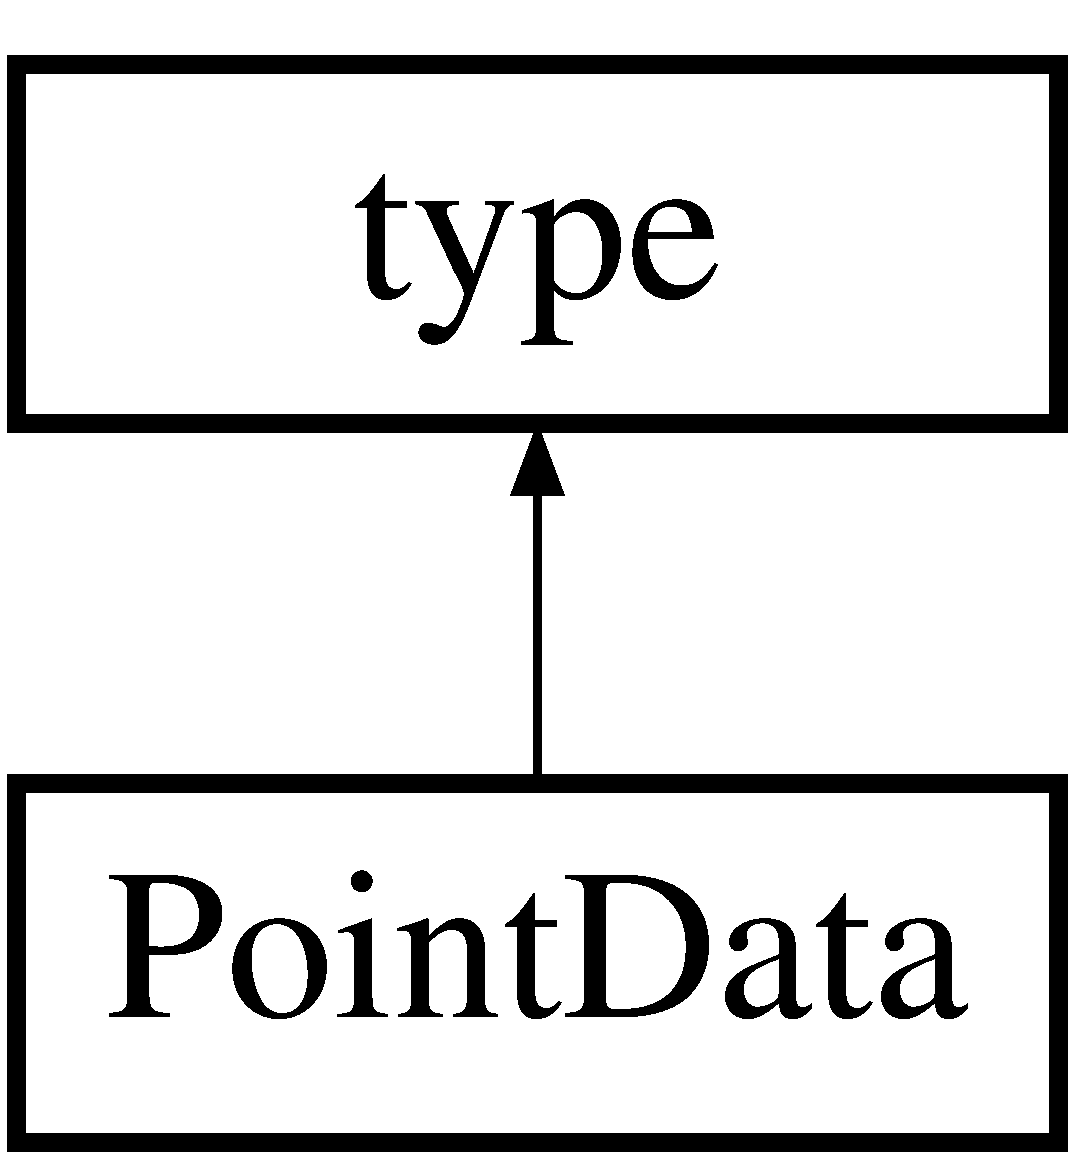
\includegraphics[height=2.000000cm]{classPointData}
\end{center}
\end{figure}
\subsection*{Public Member Functions}
\begin{DoxyCompactItemize}
\item 
virtual \hyperlink{classPointData_a53f701fd5abdb6105900c13f8282305e}{$\sim$\-Point\-Data} ()
\begin{DoxyCompactList}\small\item\em Destructor. \end{DoxyCompactList}\end{DoxyCompactItemize}
\subsection*{Data\-Array}
\label{_amgrp14411195be4ee927801b68cb96397add}%
Accessor and modifier functions for the Data\-Array sequence element. \begin{DoxyCompactItemize}
\item 
typedef \-::\hyperlink{classDataArray__t}{Data\-Array\-\_\-t} \hyperlink{classPointData_a249ad018361c7a9d61f42e1fc8af717f}{Data\-Array\-\_\-type}
\begin{DoxyCompactList}\small\item\em Element type. \end{DoxyCompactList}\item 
typedef \\*
\-::xsd\-::cxx\-::tree\-::sequence\\*
$<$ \hyperlink{classPointData_a249ad018361c7a9d61f42e1fc8af717f}{Data\-Array\-\_\-type} $>$ \hyperlink{classPointData_acd882fa412789571fcaa2599ad2b2c71}{Data\-Array\-\_\-sequence}
\begin{DoxyCompactList}\small\item\em Element sequence container type. \end{DoxyCompactList}\item 
typedef \\*
Data\-Array\-\_\-sequence\-::iterator \hyperlink{classPointData_afb66f793f2a65ca38e3cd8fa21eef701}{Data\-Array\-\_\-iterator}
\begin{DoxyCompactList}\small\item\em Element iterator type. \end{DoxyCompactList}\item 
typedef \\*
Data\-Array\-\_\-sequence\-::const\-\_\-iterator \hyperlink{classPointData_a6bd3313479b6a109e24bc9e7b306831b}{Data\-Array\-\_\-const\-\_\-iterator}
\begin{DoxyCompactList}\small\item\em Element constant iterator type. \end{DoxyCompactList}\item 
typedef \\*
\-::xsd\-::cxx\-::tree\-::traits\\*
$<$ \hyperlink{classPointData_a249ad018361c7a9d61f42e1fc8af717f}{Data\-Array\-\_\-type}, char $>$ \hyperlink{classPointData_ae9066a14984b6f7aa938ba2d58244055}{Data\-Array\-\_\-traits}
\begin{DoxyCompactList}\small\item\em Element traits type. \end{DoxyCompactList}\item 
const \hyperlink{classPointData_acd882fa412789571fcaa2599ad2b2c71}{Data\-Array\-\_\-sequence} \& \hyperlink{classPointData_ac4d75ba2976d6acdaceb0b69f574e895}{Data\-Array} () const 
\begin{DoxyCompactList}\small\item\em Return a read-\/only (constant) reference to the element sequence. \end{DoxyCompactList}\item 
\hyperlink{classPointData_acd882fa412789571fcaa2599ad2b2c71}{Data\-Array\-\_\-sequence} \& \hyperlink{classPointData_aa8ff7ad5b2c1d99794d4b96e481138d2}{Data\-Array} ()
\begin{DoxyCompactList}\small\item\em Return a read-\/write reference to the element sequence. \end{DoxyCompactList}\item 
void \hyperlink{classPointData_a207059b73203faf8b3fec8659a9104e5}{Data\-Array} (const \hyperlink{classPointData_acd882fa412789571fcaa2599ad2b2c71}{Data\-Array\-\_\-sequence} \&s)
\begin{DoxyCompactList}\small\item\em Copy elements from a given sequence. \end{DoxyCompactList}\end{DoxyCompactItemize}
\subsection*{Constructors}
\begin{DoxyCompactItemize}
\item 
\hyperlink{classPointData_add74ef42ae2c48850449cd59e216111f}{Point\-Data} ()
\begin{DoxyCompactList}\small\item\em Create an instance from the ultimate base and initializers for required elements and attributes. \end{DoxyCompactList}\item 
\hyperlink{classPointData_ae0d2a9251b2690a28a04a96105874e45}{Point\-Data} (const \-::xercesc\-::\-D\-O\-M\-Element \&e,\-::\hyperlink{namespacexml__schema_a0612287d030cb2732d31a45b258fdc87}{xml\-\_\-schema\-::flags} f=0,\-::\hyperlink{namespacexml__schema_ada9aa30dc722e93ee2ed7243085402a5}{xml\-\_\-schema\-::container} $\ast$c=0)
\begin{DoxyCompactList}\small\item\em Create an instance from a D\-O\-M element. \end{DoxyCompactList}\item 
\hyperlink{classPointData_a552557267dd3178a8e76be436b0709bc}{Point\-Data} (const \hyperlink{classPointData}{Point\-Data} \&x,\-::\hyperlink{namespacexml__schema_a0612287d030cb2732d31a45b258fdc87}{xml\-\_\-schema\-::flags} f=0,\-::\hyperlink{namespacexml__schema_ada9aa30dc722e93ee2ed7243085402a5}{xml\-\_\-schema\-::container} $\ast$c=0)
\begin{DoxyCompactList}\small\item\em Copy constructor. \end{DoxyCompactList}\item 
virtual \hyperlink{classPointData}{Point\-Data} $\ast$ \hyperlink{classPointData_aeb33ffedc35f8abc9ffd0d2f053c68ac}{\-\_\-clone} (\-::\hyperlink{namespacexml__schema_a0612287d030cb2732d31a45b258fdc87}{xml\-\_\-schema\-::flags} f=0,\-::\hyperlink{namespacexml__schema_ada9aa30dc722e93ee2ed7243085402a5}{xml\-\_\-schema\-::container} $\ast$c=0) const 
\begin{DoxyCompactList}\small\item\em Copy the instance polymorphically. \end{DoxyCompactList}\end{DoxyCompactItemize}


\subsection{Detailed Description}
Class corresponding to the Point\-Data schema type. 

\subsection{Member Typedef Documentation}
\hypertarget{classPointData_a6bd3313479b6a109e24bc9e7b306831b}{\index{Point\-Data@{Point\-Data}!Data\-Array\-\_\-const\-\_\-iterator@{Data\-Array\-\_\-const\-\_\-iterator}}
\index{Data\-Array\-\_\-const\-\_\-iterator@{Data\-Array\-\_\-const\-\_\-iterator}!PointData@{Point\-Data}}
\subsubsection[{Data\-Array\-\_\-const\-\_\-iterator}]{\setlength{\rightskip}{0pt plus 5cm}typedef Data\-Array\-\_\-sequence\-::const\-\_\-iterator {\bf Point\-Data\-::\-Data\-Array\-\_\-const\-\_\-iterator}}}\label{classPointData_a6bd3313479b6a109e24bc9e7b306831b}


Element constant iterator type. 

\hypertarget{classPointData_afb66f793f2a65ca38e3cd8fa21eef701}{\index{Point\-Data@{Point\-Data}!Data\-Array\-\_\-iterator@{Data\-Array\-\_\-iterator}}
\index{Data\-Array\-\_\-iterator@{Data\-Array\-\_\-iterator}!PointData@{Point\-Data}}
\subsubsection[{Data\-Array\-\_\-iterator}]{\setlength{\rightskip}{0pt plus 5cm}typedef Data\-Array\-\_\-sequence\-::iterator {\bf Point\-Data\-::\-Data\-Array\-\_\-iterator}}}\label{classPointData_afb66f793f2a65ca38e3cd8fa21eef701}


Element iterator type. 

\hypertarget{classPointData_acd882fa412789571fcaa2599ad2b2c71}{\index{Point\-Data@{Point\-Data}!Data\-Array\-\_\-sequence@{Data\-Array\-\_\-sequence}}
\index{Data\-Array\-\_\-sequence@{Data\-Array\-\_\-sequence}!PointData@{Point\-Data}}
\subsubsection[{Data\-Array\-\_\-sequence}]{\setlength{\rightskip}{0pt plus 5cm}typedef \-::xsd\-::cxx\-::tree\-::sequence$<$ {\bf Data\-Array\-\_\-type} $>$ {\bf Point\-Data\-::\-Data\-Array\-\_\-sequence}}}\label{classPointData_acd882fa412789571fcaa2599ad2b2c71}


Element sequence container type. 

\hypertarget{classPointData_ae9066a14984b6f7aa938ba2d58244055}{\index{Point\-Data@{Point\-Data}!Data\-Array\-\_\-traits@{Data\-Array\-\_\-traits}}
\index{Data\-Array\-\_\-traits@{Data\-Array\-\_\-traits}!PointData@{Point\-Data}}
\subsubsection[{Data\-Array\-\_\-traits}]{\setlength{\rightskip}{0pt plus 5cm}typedef \-::xsd\-::cxx\-::tree\-::traits$<$ {\bf Data\-Array\-\_\-type}, char $>$ {\bf Point\-Data\-::\-Data\-Array\-\_\-traits}}}\label{classPointData_ae9066a14984b6f7aa938ba2d58244055}


Element traits type. 

\hypertarget{classPointData_a249ad018361c7a9d61f42e1fc8af717f}{\index{Point\-Data@{Point\-Data}!Data\-Array\-\_\-type@{Data\-Array\-\_\-type}}
\index{Data\-Array\-\_\-type@{Data\-Array\-\_\-type}!PointData@{Point\-Data}}
\subsubsection[{Data\-Array\-\_\-type}]{\setlength{\rightskip}{0pt plus 5cm}typedef \-::{\bf Data\-Array\-\_\-t} {\bf Point\-Data\-::\-Data\-Array\-\_\-type}}}\label{classPointData_a249ad018361c7a9d61f42e1fc8af717f}


Element type. 



\subsection{Constructor \& Destructor Documentation}
\hypertarget{classPointData_add74ef42ae2c48850449cd59e216111f}{\index{Point\-Data@{Point\-Data}!Point\-Data@{Point\-Data}}
\index{Point\-Data@{Point\-Data}!PointData@{Point\-Data}}
\subsubsection[{Point\-Data}]{\setlength{\rightskip}{0pt plus 5cm}Point\-Data\-::\-Point\-Data (
\begin{DoxyParamCaption}
{}
\end{DoxyParamCaption}
)}}\label{classPointData_add74ef42ae2c48850449cd59e216111f}


Create an instance from the ultimate base and initializers for required elements and attributes. 

\hypertarget{classPointData_ae0d2a9251b2690a28a04a96105874e45}{\index{Point\-Data@{Point\-Data}!Point\-Data@{Point\-Data}}
\index{Point\-Data@{Point\-Data}!PointData@{Point\-Data}}
\subsubsection[{Point\-Data}]{\setlength{\rightskip}{0pt plus 5cm}Point\-Data\-::\-Point\-Data (
\begin{DoxyParamCaption}
\item[{const \-::xercesc\-::\-D\-O\-M\-Element \&}]{e, }
\item[{\-::{\bf xml\-\_\-schema\-::flags}}]{f = {\ttfamily 0}, }
\item[{\-::{\bf xml\-\_\-schema\-::container} $\ast$}]{c = {\ttfamily 0}}
\end{DoxyParamCaption}
)}}\label{classPointData_ae0d2a9251b2690a28a04a96105874e45}


Create an instance from a D\-O\-M element. 


\begin{DoxyParams}{Parameters}
{\em e} & A D\-O\-M element to extract the data from. \\
\hline
{\em f} & Flags to create the new instance with. \\
\hline
{\em c} & A pointer to the object that will contain the new instance. \\
\hline
\end{DoxyParams}
\hypertarget{classPointData_a552557267dd3178a8e76be436b0709bc}{\index{Point\-Data@{Point\-Data}!Point\-Data@{Point\-Data}}
\index{Point\-Data@{Point\-Data}!PointData@{Point\-Data}}
\subsubsection[{Point\-Data}]{\setlength{\rightskip}{0pt plus 5cm}Point\-Data\-::\-Point\-Data (
\begin{DoxyParamCaption}
\item[{const {\bf Point\-Data} \&}]{x, }
\item[{\-::{\bf xml\-\_\-schema\-::flags}}]{f = {\ttfamily 0}, }
\item[{\-::{\bf xml\-\_\-schema\-::container} $\ast$}]{c = {\ttfamily 0}}
\end{DoxyParamCaption}
)}}\label{classPointData_a552557267dd3178a8e76be436b0709bc}


Copy constructor. 


\begin{DoxyParams}{Parameters}
{\em x} & An instance to make a copy of. \\
\hline
{\em f} & Flags to create the copy with. \\
\hline
{\em c} & A pointer to the object that will contain the copy.\\
\hline
\end{DoxyParams}
For polymorphic object models use the {\ttfamily \-\_\-clone} function instead. \hypertarget{classPointData_a53f701fd5abdb6105900c13f8282305e}{\index{Point\-Data@{Point\-Data}!$\sim$\-Point\-Data@{$\sim$\-Point\-Data}}
\index{$\sim$\-Point\-Data@{$\sim$\-Point\-Data}!PointData@{Point\-Data}}
\subsubsection[{$\sim$\-Point\-Data}]{\setlength{\rightskip}{0pt plus 5cm}Point\-Data\-::$\sim$\-Point\-Data (
\begin{DoxyParamCaption}
{}
\end{DoxyParamCaption}
)\hspace{0.3cm}{\ttfamily [virtual]}}}\label{classPointData_a53f701fd5abdb6105900c13f8282305e}


Destructor. 



\subsection{Member Function Documentation}
\hypertarget{classPointData_aeb33ffedc35f8abc9ffd0d2f053c68ac}{\index{Point\-Data@{Point\-Data}!\-\_\-clone@{\-\_\-clone}}
\index{\-\_\-clone@{\-\_\-clone}!PointData@{Point\-Data}}
\subsubsection[{\-\_\-clone}]{\setlength{\rightskip}{0pt plus 5cm}{\bf Point\-Data} $\ast$ Point\-Data\-::\-\_\-clone (
\begin{DoxyParamCaption}
\item[{\-::{\bf xml\-\_\-schema\-::flags}}]{f = {\ttfamily 0}, }
\item[{\-::{\bf xml\-\_\-schema\-::container} $\ast$}]{c = {\ttfamily 0}}
\end{DoxyParamCaption}
) const\hspace{0.3cm}{\ttfamily [virtual]}}}\label{classPointData_aeb33ffedc35f8abc9ffd0d2f053c68ac}


Copy the instance polymorphically. 


\begin{DoxyParams}{Parameters}
{\em f} & Flags to create the copy with. \\
\hline
{\em c} & A pointer to the object that will contain the copy. \\
\hline
\end{DoxyParams}
\begin{DoxyReturn}{Returns}
A pointer to the dynamically allocated copy.
\end{DoxyReturn}
This function ensures that the dynamic type of the instance is used for copying and should be used for polymorphic object models instead of the copy constructor. \hypertarget{classPointData_ac4d75ba2976d6acdaceb0b69f574e895}{\index{Point\-Data@{Point\-Data}!Data\-Array@{Data\-Array}}
\index{Data\-Array@{Data\-Array}!PointData@{Point\-Data}}
\subsubsection[{Data\-Array}]{\setlength{\rightskip}{0pt plus 5cm}const {\bf Point\-Data\-::\-Data\-Array\-\_\-sequence} \& Point\-Data\-::\-Data\-Array (
\begin{DoxyParamCaption}
{}
\end{DoxyParamCaption}
) const}}\label{classPointData_ac4d75ba2976d6acdaceb0b69f574e895}


Return a read-\/only (constant) reference to the element sequence. 

\begin{DoxyReturn}{Returns}
A constant reference to the sequence container. 
\end{DoxyReturn}
\hypertarget{classPointData_aa8ff7ad5b2c1d99794d4b96e481138d2}{\index{Point\-Data@{Point\-Data}!Data\-Array@{Data\-Array}}
\index{Data\-Array@{Data\-Array}!PointData@{Point\-Data}}
\subsubsection[{Data\-Array}]{\setlength{\rightskip}{0pt plus 5cm}{\bf Point\-Data\-::\-Data\-Array\-\_\-sequence} \& Point\-Data\-::\-Data\-Array (
\begin{DoxyParamCaption}
{}
\end{DoxyParamCaption}
)}}\label{classPointData_aa8ff7ad5b2c1d99794d4b96e481138d2}


Return a read-\/write reference to the element sequence. 

\begin{DoxyReturn}{Returns}
A reference to the sequence container. 
\end{DoxyReturn}
\hypertarget{classPointData_a207059b73203faf8b3fec8659a9104e5}{\index{Point\-Data@{Point\-Data}!Data\-Array@{Data\-Array}}
\index{Data\-Array@{Data\-Array}!PointData@{Point\-Data}}
\subsubsection[{Data\-Array}]{\setlength{\rightskip}{0pt plus 5cm}void Point\-Data\-::\-Data\-Array (
\begin{DoxyParamCaption}
\item[{const {\bf Data\-Array\-\_\-sequence} \&}]{s}
\end{DoxyParamCaption}
)}}\label{classPointData_a207059b73203faf8b3fec8659a9104e5}


Copy elements from a given sequence. 


\begin{DoxyParams}{Parameters}
{\em s} & A sequence to copy elements from.\\
\hline
\end{DoxyParams}
For each element in {\itshape s} this function makes a copy and adds it to the sequence. Note that this operation completely changes the sequence and all old elements will be lost. 

The documentation for this class was generated from the following files\-:\begin{DoxyCompactItemize}
\item 
src/output\-Writer/\hyperlink{vtk-unstructured_8h}{vtk-\/unstructured.\-h}\item 
src/output\-Writer/\hyperlink{vtk-unstructured_8cpp}{vtk-\/unstructured.\-cpp}\end{DoxyCompactItemize}

\hypertarget{classPoints}{\section{Points Class Reference}
\label{classPoints}\index{Points@{Points}}
}


Class corresponding to the Points schema type.  




{\ttfamily \#include $<$vtk-\/unstructured.\-h$>$}

Inheritance diagram for Points\-:\begin{figure}[H]
\begin{center}
\leavevmode
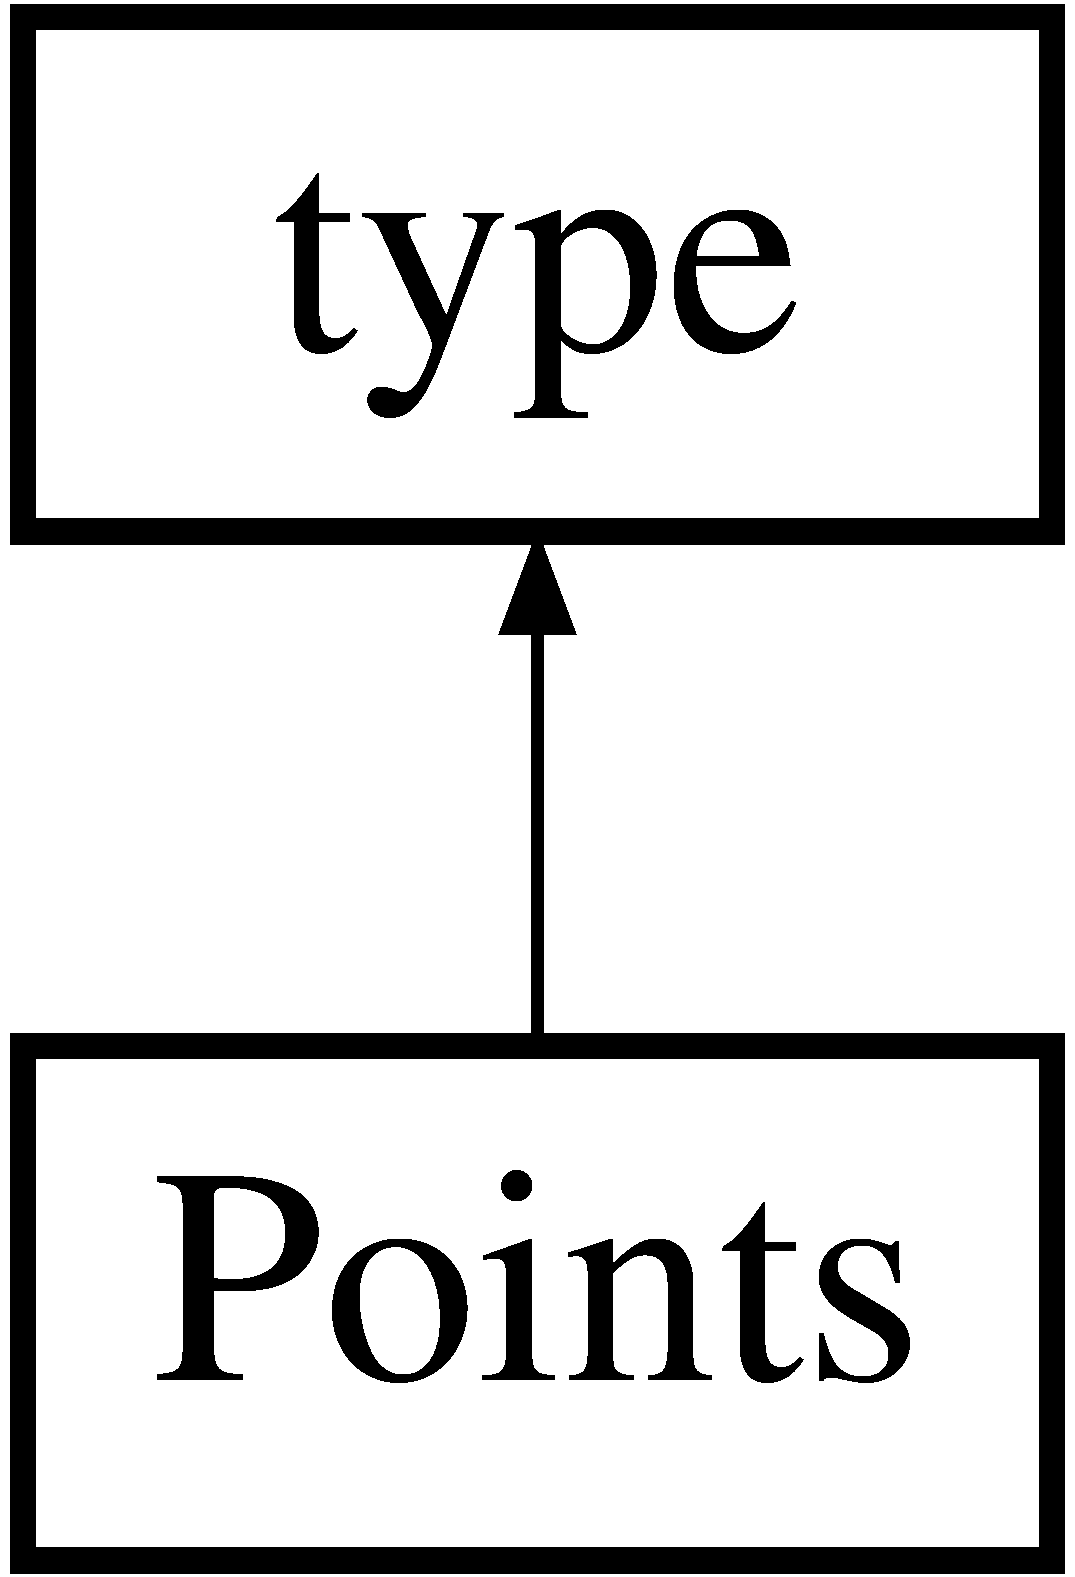
\includegraphics[height=2.000000cm]{classPoints}
\end{center}
\end{figure}
\subsection*{Public Member Functions}
\begin{DoxyCompactItemize}
\item 
virtual \hyperlink{classPoints_a9d56d7dc8b6a6f492e07d354eb379c12}{$\sim$\-Points} ()
\begin{DoxyCompactList}\small\item\em Destructor. \end{DoxyCompactList}\end{DoxyCompactItemize}
\subsection*{Data\-Array}
\label{_amgrp14411195be4ee927801b68cb96397add}%
Accessor and modifier functions for the Data\-Array sequence element. \begin{DoxyCompactItemize}
\item 
typedef \-::\hyperlink{classDataArray__t}{Data\-Array\-\_\-t} \hyperlink{classPoints_a6afedf501b722fe7d7ffeae03ece6238}{Data\-Array\-\_\-type}
\begin{DoxyCompactList}\small\item\em Element type. \end{DoxyCompactList}\item 
typedef \\*
\-::xsd\-::cxx\-::tree\-::sequence\\*
$<$ \hyperlink{classPoints_a6afedf501b722fe7d7ffeae03ece6238}{Data\-Array\-\_\-type} $>$ \hyperlink{classPoints_ac8b51dcf0e7659ca61ff9b9d24051016}{Data\-Array\-\_\-sequence}
\begin{DoxyCompactList}\small\item\em Element sequence container type. \end{DoxyCompactList}\item 
typedef \\*
Data\-Array\-\_\-sequence\-::iterator \hyperlink{classPoints_ac4cd7a177b464c1e08d493600a7e6e16}{Data\-Array\-\_\-iterator}
\begin{DoxyCompactList}\small\item\em Element iterator type. \end{DoxyCompactList}\item 
typedef \\*
Data\-Array\-\_\-sequence\-::const\-\_\-iterator \hyperlink{classPoints_a795a395909c3360569fe0e854ba6059e}{Data\-Array\-\_\-const\-\_\-iterator}
\begin{DoxyCompactList}\small\item\em Element constant iterator type. \end{DoxyCompactList}\item 
typedef \\*
\-::xsd\-::cxx\-::tree\-::traits\\*
$<$ \hyperlink{classPoints_a6afedf501b722fe7d7ffeae03ece6238}{Data\-Array\-\_\-type}, char $>$ \hyperlink{classPoints_a815b88c9204c7251f4a08c6769645ef1}{Data\-Array\-\_\-traits}
\begin{DoxyCompactList}\small\item\em Element traits type. \end{DoxyCompactList}\item 
const \hyperlink{classPoints_ac8b51dcf0e7659ca61ff9b9d24051016}{Data\-Array\-\_\-sequence} \& \hyperlink{classPoints_a86c60a0068ebdb8d3e8cbe9fa8f35f55}{Data\-Array} () const 
\begin{DoxyCompactList}\small\item\em Return a read-\/only (constant) reference to the element sequence. \end{DoxyCompactList}\item 
\hyperlink{classPoints_ac8b51dcf0e7659ca61ff9b9d24051016}{Data\-Array\-\_\-sequence} \& \hyperlink{classPoints_a3fdfb1b1b2f1221ad50ba5087826177c}{Data\-Array} ()
\begin{DoxyCompactList}\small\item\em Return a read-\/write reference to the element sequence. \end{DoxyCompactList}\item 
void \hyperlink{classPoints_aa22a86fe31d5f903be59dda3de92bb67}{Data\-Array} (const \hyperlink{classPoints_ac8b51dcf0e7659ca61ff9b9d24051016}{Data\-Array\-\_\-sequence} \&s)
\begin{DoxyCompactList}\small\item\em Copy elements from a given sequence. \end{DoxyCompactList}\end{DoxyCompactItemize}
\subsection*{Constructors}
\begin{DoxyCompactItemize}
\item 
\hyperlink{classPoints_aa4e68083d98bd04233c9753dfe1e46ab}{Points} ()
\begin{DoxyCompactList}\small\item\em Create an instance from the ultimate base and initializers for required elements and attributes. \end{DoxyCompactList}\item 
\hyperlink{classPoints_a36a1ac8ea9ac092adff2888915e81304}{Points} (const \-::xercesc\-::\-D\-O\-M\-Element \&e,\-::\hyperlink{namespacexml__schema_a0612287d030cb2732d31a45b258fdc87}{xml\-\_\-schema\-::flags} f=0,\-::\hyperlink{namespacexml__schema_ada9aa30dc722e93ee2ed7243085402a5}{xml\-\_\-schema\-::container} $\ast$c=0)
\begin{DoxyCompactList}\small\item\em Create an instance from a D\-O\-M element. \end{DoxyCompactList}\item 
\hyperlink{classPoints_ad49b51469dc53b028c244a88bd9fb08b}{Points} (const \hyperlink{classPoints}{Points} \&x,\-::\hyperlink{namespacexml__schema_a0612287d030cb2732d31a45b258fdc87}{xml\-\_\-schema\-::flags} f=0,\-::\hyperlink{namespacexml__schema_ada9aa30dc722e93ee2ed7243085402a5}{xml\-\_\-schema\-::container} $\ast$c=0)
\begin{DoxyCompactList}\small\item\em Copy constructor. \end{DoxyCompactList}\item 
virtual \hyperlink{classPoints}{Points} $\ast$ \hyperlink{classPoints_a5dff673c4b4a59465aee3ede80328ae9}{\-\_\-clone} (\-::\hyperlink{namespacexml__schema_a0612287d030cb2732d31a45b258fdc87}{xml\-\_\-schema\-::flags} f=0,\-::\hyperlink{namespacexml__schema_ada9aa30dc722e93ee2ed7243085402a5}{xml\-\_\-schema\-::container} $\ast$c=0) const 
\begin{DoxyCompactList}\small\item\em Copy the instance polymorphically. \end{DoxyCompactList}\end{DoxyCompactItemize}


\subsection{Detailed Description}
Class corresponding to the Points schema type. 

\subsection{Member Typedef Documentation}
\hypertarget{classPoints_a795a395909c3360569fe0e854ba6059e}{\index{Points@{Points}!Data\-Array\-\_\-const\-\_\-iterator@{Data\-Array\-\_\-const\-\_\-iterator}}
\index{Data\-Array\-\_\-const\-\_\-iterator@{Data\-Array\-\_\-const\-\_\-iterator}!Points@{Points}}
\subsubsection[{Data\-Array\-\_\-const\-\_\-iterator}]{\setlength{\rightskip}{0pt plus 5cm}typedef Data\-Array\-\_\-sequence\-::const\-\_\-iterator {\bf Points\-::\-Data\-Array\-\_\-const\-\_\-iterator}}}\label{classPoints_a795a395909c3360569fe0e854ba6059e}


Element constant iterator type. 

\hypertarget{classPoints_ac4cd7a177b464c1e08d493600a7e6e16}{\index{Points@{Points}!Data\-Array\-\_\-iterator@{Data\-Array\-\_\-iterator}}
\index{Data\-Array\-\_\-iterator@{Data\-Array\-\_\-iterator}!Points@{Points}}
\subsubsection[{Data\-Array\-\_\-iterator}]{\setlength{\rightskip}{0pt plus 5cm}typedef Data\-Array\-\_\-sequence\-::iterator {\bf Points\-::\-Data\-Array\-\_\-iterator}}}\label{classPoints_ac4cd7a177b464c1e08d493600a7e6e16}


Element iterator type. 

\hypertarget{classPoints_ac8b51dcf0e7659ca61ff9b9d24051016}{\index{Points@{Points}!Data\-Array\-\_\-sequence@{Data\-Array\-\_\-sequence}}
\index{Data\-Array\-\_\-sequence@{Data\-Array\-\_\-sequence}!Points@{Points}}
\subsubsection[{Data\-Array\-\_\-sequence}]{\setlength{\rightskip}{0pt plus 5cm}typedef \-::xsd\-::cxx\-::tree\-::sequence$<$ {\bf Data\-Array\-\_\-type} $>$ {\bf Points\-::\-Data\-Array\-\_\-sequence}}}\label{classPoints_ac8b51dcf0e7659ca61ff9b9d24051016}


Element sequence container type. 

\hypertarget{classPoints_a815b88c9204c7251f4a08c6769645ef1}{\index{Points@{Points}!Data\-Array\-\_\-traits@{Data\-Array\-\_\-traits}}
\index{Data\-Array\-\_\-traits@{Data\-Array\-\_\-traits}!Points@{Points}}
\subsubsection[{Data\-Array\-\_\-traits}]{\setlength{\rightskip}{0pt plus 5cm}typedef \-::xsd\-::cxx\-::tree\-::traits$<$ {\bf Data\-Array\-\_\-type}, char $>$ {\bf Points\-::\-Data\-Array\-\_\-traits}}}\label{classPoints_a815b88c9204c7251f4a08c6769645ef1}


Element traits type. 

\hypertarget{classPoints_a6afedf501b722fe7d7ffeae03ece6238}{\index{Points@{Points}!Data\-Array\-\_\-type@{Data\-Array\-\_\-type}}
\index{Data\-Array\-\_\-type@{Data\-Array\-\_\-type}!Points@{Points}}
\subsubsection[{Data\-Array\-\_\-type}]{\setlength{\rightskip}{0pt plus 5cm}typedef \-::{\bf Data\-Array\-\_\-t} {\bf Points\-::\-Data\-Array\-\_\-type}}}\label{classPoints_a6afedf501b722fe7d7ffeae03ece6238}


Element type. 



\subsection{Constructor \& Destructor Documentation}
\hypertarget{classPoints_aa4e68083d98bd04233c9753dfe1e46ab}{\index{Points@{Points}!Points@{Points}}
\index{Points@{Points}!Points@{Points}}
\subsubsection[{Points}]{\setlength{\rightskip}{0pt plus 5cm}Points\-::\-Points (
\begin{DoxyParamCaption}
{}
\end{DoxyParamCaption}
)}}\label{classPoints_aa4e68083d98bd04233c9753dfe1e46ab}


Create an instance from the ultimate base and initializers for required elements and attributes. 

\hypertarget{classPoints_a36a1ac8ea9ac092adff2888915e81304}{\index{Points@{Points}!Points@{Points}}
\index{Points@{Points}!Points@{Points}}
\subsubsection[{Points}]{\setlength{\rightskip}{0pt plus 5cm}Points\-::\-Points (
\begin{DoxyParamCaption}
\item[{const \-::xercesc\-::\-D\-O\-M\-Element \&}]{e, }
\item[{\-::{\bf xml\-\_\-schema\-::flags}}]{f = {\ttfamily 0}, }
\item[{\-::{\bf xml\-\_\-schema\-::container} $\ast$}]{c = {\ttfamily 0}}
\end{DoxyParamCaption}
)}}\label{classPoints_a36a1ac8ea9ac092adff2888915e81304}


Create an instance from a D\-O\-M element. 


\begin{DoxyParams}{Parameters}
{\em e} & A D\-O\-M element to extract the data from. \\
\hline
{\em f} & Flags to create the new instance with. \\
\hline
{\em c} & A pointer to the object that will contain the new instance. \\
\hline
\end{DoxyParams}
\hypertarget{classPoints_ad49b51469dc53b028c244a88bd9fb08b}{\index{Points@{Points}!Points@{Points}}
\index{Points@{Points}!Points@{Points}}
\subsubsection[{Points}]{\setlength{\rightskip}{0pt plus 5cm}Points\-::\-Points (
\begin{DoxyParamCaption}
\item[{const {\bf Points} \&}]{x, }
\item[{\-::{\bf xml\-\_\-schema\-::flags}}]{f = {\ttfamily 0}, }
\item[{\-::{\bf xml\-\_\-schema\-::container} $\ast$}]{c = {\ttfamily 0}}
\end{DoxyParamCaption}
)}}\label{classPoints_ad49b51469dc53b028c244a88bd9fb08b}


Copy constructor. 


\begin{DoxyParams}{Parameters}
{\em x} & An instance to make a copy of. \\
\hline
{\em f} & Flags to create the copy with. \\
\hline
{\em c} & A pointer to the object that will contain the copy.\\
\hline
\end{DoxyParams}
For polymorphic object models use the {\ttfamily \-\_\-clone} function instead. \hypertarget{classPoints_a9d56d7dc8b6a6f492e07d354eb379c12}{\index{Points@{Points}!$\sim$\-Points@{$\sim$\-Points}}
\index{$\sim$\-Points@{$\sim$\-Points}!Points@{Points}}
\subsubsection[{$\sim$\-Points}]{\setlength{\rightskip}{0pt plus 5cm}Points\-::$\sim$\-Points (
\begin{DoxyParamCaption}
{}
\end{DoxyParamCaption}
)\hspace{0.3cm}{\ttfamily [virtual]}}}\label{classPoints_a9d56d7dc8b6a6f492e07d354eb379c12}


Destructor. 



\subsection{Member Function Documentation}
\hypertarget{classPoints_a5dff673c4b4a59465aee3ede80328ae9}{\index{Points@{Points}!\-\_\-clone@{\-\_\-clone}}
\index{\-\_\-clone@{\-\_\-clone}!Points@{Points}}
\subsubsection[{\-\_\-clone}]{\setlength{\rightskip}{0pt plus 5cm}{\bf Points} $\ast$ Points\-::\-\_\-clone (
\begin{DoxyParamCaption}
\item[{\-::{\bf xml\-\_\-schema\-::flags}}]{f = {\ttfamily 0}, }
\item[{\-::{\bf xml\-\_\-schema\-::container} $\ast$}]{c = {\ttfamily 0}}
\end{DoxyParamCaption}
) const\hspace{0.3cm}{\ttfamily [virtual]}}}\label{classPoints_a5dff673c4b4a59465aee3ede80328ae9}


Copy the instance polymorphically. 


\begin{DoxyParams}{Parameters}
{\em f} & Flags to create the copy with. \\
\hline
{\em c} & A pointer to the object that will contain the copy. \\
\hline
\end{DoxyParams}
\begin{DoxyReturn}{Returns}
A pointer to the dynamically allocated copy.
\end{DoxyReturn}
This function ensures that the dynamic type of the instance is used for copying and should be used for polymorphic object models instead of the copy constructor. \hypertarget{classPoints_a86c60a0068ebdb8d3e8cbe9fa8f35f55}{\index{Points@{Points}!Data\-Array@{Data\-Array}}
\index{Data\-Array@{Data\-Array}!Points@{Points}}
\subsubsection[{Data\-Array}]{\setlength{\rightskip}{0pt plus 5cm}const {\bf Points\-::\-Data\-Array\-\_\-sequence} \& Points\-::\-Data\-Array (
\begin{DoxyParamCaption}
{}
\end{DoxyParamCaption}
) const}}\label{classPoints_a86c60a0068ebdb8d3e8cbe9fa8f35f55}


Return a read-\/only (constant) reference to the element sequence. 

\begin{DoxyReturn}{Returns}
A constant reference to the sequence container. 
\end{DoxyReturn}
\hypertarget{classPoints_a3fdfb1b1b2f1221ad50ba5087826177c}{\index{Points@{Points}!Data\-Array@{Data\-Array}}
\index{Data\-Array@{Data\-Array}!Points@{Points}}
\subsubsection[{Data\-Array}]{\setlength{\rightskip}{0pt plus 5cm}{\bf Points\-::\-Data\-Array\-\_\-sequence} \& Points\-::\-Data\-Array (
\begin{DoxyParamCaption}
{}
\end{DoxyParamCaption}
)}}\label{classPoints_a3fdfb1b1b2f1221ad50ba5087826177c}


Return a read-\/write reference to the element sequence. 

\begin{DoxyReturn}{Returns}
A reference to the sequence container. 
\end{DoxyReturn}
\hypertarget{classPoints_aa22a86fe31d5f903be59dda3de92bb67}{\index{Points@{Points}!Data\-Array@{Data\-Array}}
\index{Data\-Array@{Data\-Array}!Points@{Points}}
\subsubsection[{Data\-Array}]{\setlength{\rightskip}{0pt plus 5cm}void Points\-::\-Data\-Array (
\begin{DoxyParamCaption}
\item[{const {\bf Data\-Array\-\_\-sequence} \&}]{s}
\end{DoxyParamCaption}
)}}\label{classPoints_aa22a86fe31d5f903be59dda3de92bb67}


Copy elements from a given sequence. 


\begin{DoxyParams}{Parameters}
{\em s} & A sequence to copy elements from.\\
\hline
\end{DoxyParams}
For each element in {\itshape s} this function makes a copy and adds it to the sequence. Note that this operation completely changes the sequence and all old elements will be lost. 

The documentation for this class was generated from the following files\-:\begin{DoxyCompactItemize}
\item 
src/output\-Writer/\hyperlink{vtk-unstructured_8h}{vtk-\/unstructured.\-h}\item 
src/output\-Writer/\hyperlink{vtk-unstructured_8cpp}{vtk-\/unstructured.\-cpp}\end{DoxyCompactItemize}

\hypertarget{classPolyData__t}{\section{Poly\-Data\-\_\-t Class Reference}
\label{classPolyData__t}\index{Poly\-Data\-\_\-t@{Poly\-Data\-\_\-t}}
}


Class corresponding to the Poly\-Data\-\_\-t schema type.  




{\ttfamily \#include $<$vtk-\/unstructured.\-h$>$}

Inheritance diagram for Poly\-Data\-\_\-t\-:\begin{figure}[H]
\begin{center}
\leavevmode
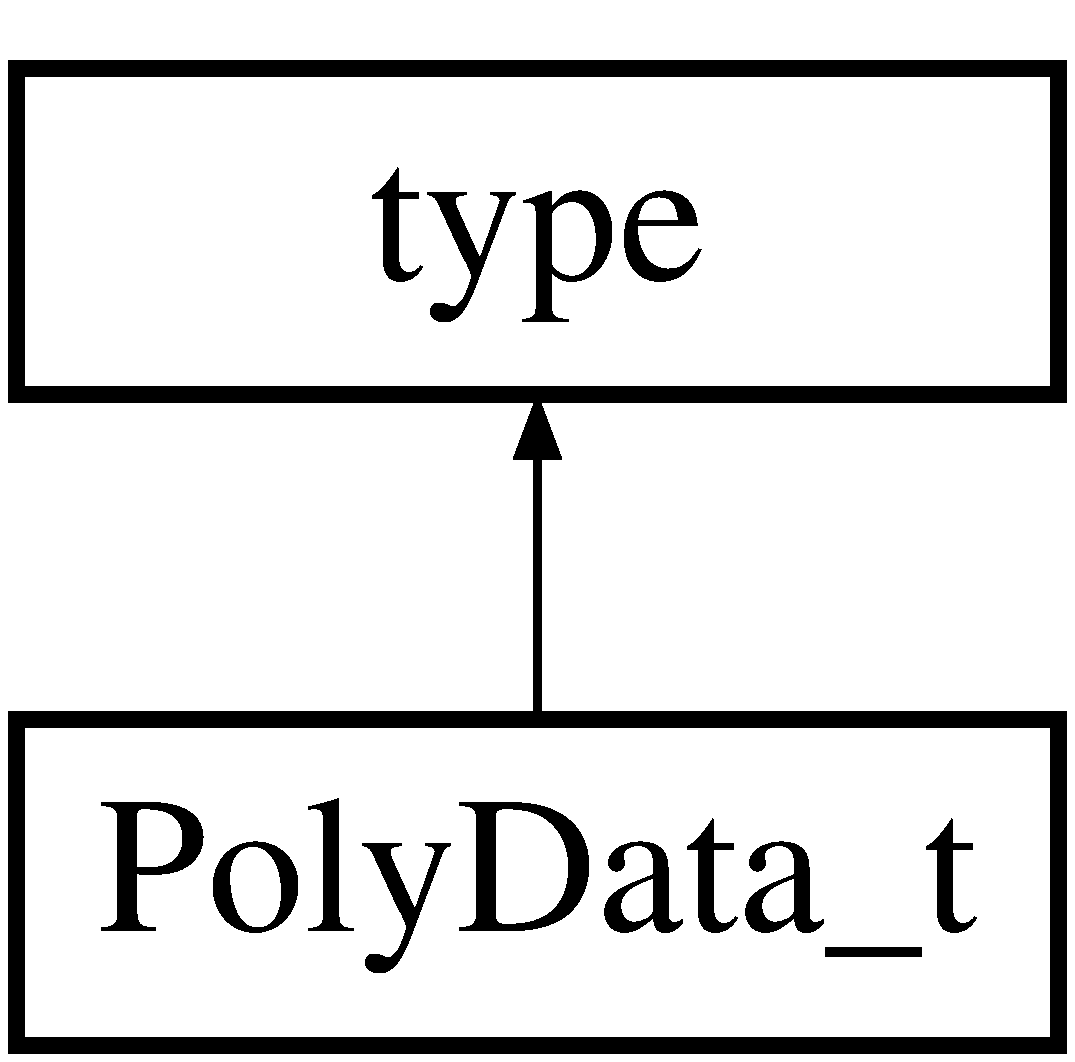
\includegraphics[height=2.000000cm]{classPolyData__t}
\end{center}
\end{figure}
\subsection*{Public Member Functions}
\begin{DoxyCompactItemize}
\item 
virtual \hyperlink{classPolyData__t_afefe18d998d21a0557e30c06b4089b99}{$\sim$\-Poly\-Data\-\_\-t} ()
\begin{DoxyCompactList}\small\item\em Destructor. \end{DoxyCompactList}\end{DoxyCompactItemize}
\subsection*{greeting}
\label{_amgrp699e0311097c48b46019dcfc07c772a1}%
Accessor and modifier functions for the greeting required element. \begin{DoxyCompactItemize}
\item 
typedef \-::\hyperlink{namespacexml__schema_ac0cec83a330f0024e4e318b3deac5104}{xml\-\_\-schema\-::string} \hyperlink{classPolyData__t_ae1f86bd7b6a37a0d0851de8a44627177}{greeting\-\_\-type}
\begin{DoxyCompactList}\small\item\em Element type. \end{DoxyCompactList}\item 
typedef \\*
\-::xsd\-::cxx\-::tree\-::traits\\*
$<$ \hyperlink{classPolyData__t_ae1f86bd7b6a37a0d0851de8a44627177}{greeting\-\_\-type}, char $>$ \hyperlink{classPolyData__t_a0825d12eafceffcedbb147730b8bf8a6}{greeting\-\_\-traits}
\begin{DoxyCompactList}\small\item\em Element traits type. \end{DoxyCompactList}\item 
const \hyperlink{classPolyData__t_ae1f86bd7b6a37a0d0851de8a44627177}{greeting\-\_\-type} \& \hyperlink{classPolyData__t_acce3e6cf99db0b383320a0ccfd62789f}{greeting} () const 
\begin{DoxyCompactList}\small\item\em Return a read-\/only (constant) reference to the element. \end{DoxyCompactList}\item 
\hyperlink{classPolyData__t_ae1f86bd7b6a37a0d0851de8a44627177}{greeting\-\_\-type} \& \hyperlink{classPolyData__t_a3879d9f3b0b8ae707f1c2465bbbcf507}{greeting} ()
\begin{DoxyCompactList}\small\item\em Return a read-\/write reference to the element. \end{DoxyCompactList}\item 
void \hyperlink{classPolyData__t_a23d6e1490860af1f76f135efb37510e1}{greeting} (const \hyperlink{classPolyData__t_ae1f86bd7b6a37a0d0851de8a44627177}{greeting\-\_\-type} \&x)
\begin{DoxyCompactList}\small\item\em Set the element value. \end{DoxyCompactList}\item 
void \hyperlink{classPolyData__t_a27c66fbcb156a64615e29b1082facd00}{greeting} (\-::std\-::auto\-\_\-ptr$<$ \hyperlink{classPolyData__t_ae1f86bd7b6a37a0d0851de8a44627177}{greeting\-\_\-type} $>$ p)
\begin{DoxyCompactList}\small\item\em Set the element value without copying. \end{DoxyCompactList}\end{DoxyCompactItemize}
\subsection*{Constructors}
\begin{DoxyCompactItemize}
\item 
\hyperlink{classPolyData__t_a4da6cc1205eee54feaebde53665f0621}{Poly\-Data\-\_\-t} (const \hyperlink{classPolyData__t_ae1f86bd7b6a37a0d0851de8a44627177}{greeting\-\_\-type} \&)
\begin{DoxyCompactList}\small\item\em Create an instance from the ultimate base and initializers for required elements and attributes. \end{DoxyCompactList}\item 
\hyperlink{classPolyData__t_a47b921cff0546cc9502c008a219d0058}{Poly\-Data\-\_\-t} (const \-::xercesc\-::\-D\-O\-M\-Element \&e,\-::\hyperlink{namespacexml__schema_a0612287d030cb2732d31a45b258fdc87}{xml\-\_\-schema\-::flags} f=0,\-::\hyperlink{namespacexml__schema_ada9aa30dc722e93ee2ed7243085402a5}{xml\-\_\-schema\-::container} $\ast$c=0)
\begin{DoxyCompactList}\small\item\em Create an instance from a D\-O\-M element. \end{DoxyCompactList}\item 
\hyperlink{classPolyData__t_a6a0cccceec7668fe2f28776a4898a009}{Poly\-Data\-\_\-t} (const \hyperlink{classPolyData__t}{Poly\-Data\-\_\-t} \&x,\-::\hyperlink{namespacexml__schema_a0612287d030cb2732d31a45b258fdc87}{xml\-\_\-schema\-::flags} f=0,\-::\hyperlink{namespacexml__schema_ada9aa30dc722e93ee2ed7243085402a5}{xml\-\_\-schema\-::container} $\ast$c=0)
\begin{DoxyCompactList}\small\item\em Copy constructor. \end{DoxyCompactList}\item 
virtual \hyperlink{classPolyData__t}{Poly\-Data\-\_\-t} $\ast$ \hyperlink{classPolyData__t_a90079722e663d849db7dec71493ddffe}{\-\_\-clone} (\-::\hyperlink{namespacexml__schema_a0612287d030cb2732d31a45b258fdc87}{xml\-\_\-schema\-::flags} f=0,\-::\hyperlink{namespacexml__schema_ada9aa30dc722e93ee2ed7243085402a5}{xml\-\_\-schema\-::container} $\ast$c=0) const 
\begin{DoxyCompactList}\small\item\em Copy the instance polymorphically. \end{DoxyCompactList}\end{DoxyCompactItemize}


\subsection{Detailed Description}
Class corresponding to the Poly\-Data\-\_\-t schema type. 

\subsection{Member Typedef Documentation}
\hypertarget{classPolyData__t_a0825d12eafceffcedbb147730b8bf8a6}{\index{Poly\-Data\-\_\-t@{Poly\-Data\-\_\-t}!greeting\-\_\-traits@{greeting\-\_\-traits}}
\index{greeting\-\_\-traits@{greeting\-\_\-traits}!PolyData_t@{Poly\-Data\-\_\-t}}
\subsubsection[{greeting\-\_\-traits}]{\setlength{\rightskip}{0pt plus 5cm}typedef \-::xsd\-::cxx\-::tree\-::traits$<$ {\bf greeting\-\_\-type}, char $>$ {\bf Poly\-Data\-\_\-t\-::greeting\-\_\-traits}}}\label{classPolyData__t_a0825d12eafceffcedbb147730b8bf8a6}


Element traits type. 

\hypertarget{classPolyData__t_ae1f86bd7b6a37a0d0851de8a44627177}{\index{Poly\-Data\-\_\-t@{Poly\-Data\-\_\-t}!greeting\-\_\-type@{greeting\-\_\-type}}
\index{greeting\-\_\-type@{greeting\-\_\-type}!PolyData_t@{Poly\-Data\-\_\-t}}
\subsubsection[{greeting\-\_\-type}]{\setlength{\rightskip}{0pt plus 5cm}typedef \-::{\bf xml\-\_\-schema\-::string} {\bf Poly\-Data\-\_\-t\-::greeting\-\_\-type}}}\label{classPolyData__t_ae1f86bd7b6a37a0d0851de8a44627177}


Element type. 



\subsection{Constructor \& Destructor Documentation}
\hypertarget{classPolyData__t_a4da6cc1205eee54feaebde53665f0621}{\index{Poly\-Data\-\_\-t@{Poly\-Data\-\_\-t}!Poly\-Data\-\_\-t@{Poly\-Data\-\_\-t}}
\index{Poly\-Data\-\_\-t@{Poly\-Data\-\_\-t}!PolyData_t@{Poly\-Data\-\_\-t}}
\subsubsection[{Poly\-Data\-\_\-t}]{\setlength{\rightskip}{0pt plus 5cm}Poly\-Data\-\_\-t\-::\-Poly\-Data\-\_\-t (
\begin{DoxyParamCaption}
\item[{const {\bf greeting\-\_\-type} \&}]{greeting}
\end{DoxyParamCaption}
)}}\label{classPolyData__t_a4da6cc1205eee54feaebde53665f0621}


Create an instance from the ultimate base and initializers for required elements and attributes. 

\hypertarget{classPolyData__t_a47b921cff0546cc9502c008a219d0058}{\index{Poly\-Data\-\_\-t@{Poly\-Data\-\_\-t}!Poly\-Data\-\_\-t@{Poly\-Data\-\_\-t}}
\index{Poly\-Data\-\_\-t@{Poly\-Data\-\_\-t}!PolyData_t@{Poly\-Data\-\_\-t}}
\subsubsection[{Poly\-Data\-\_\-t}]{\setlength{\rightskip}{0pt plus 5cm}Poly\-Data\-\_\-t\-::\-Poly\-Data\-\_\-t (
\begin{DoxyParamCaption}
\item[{const \-::xercesc\-::\-D\-O\-M\-Element \&}]{e, }
\item[{\-::{\bf xml\-\_\-schema\-::flags}}]{f = {\ttfamily 0}, }
\item[{\-::{\bf xml\-\_\-schema\-::container} $\ast$}]{c = {\ttfamily 0}}
\end{DoxyParamCaption}
)}}\label{classPolyData__t_a47b921cff0546cc9502c008a219d0058}


Create an instance from a D\-O\-M element. 


\begin{DoxyParams}{Parameters}
{\em e} & A D\-O\-M element to extract the data from. \\
\hline
{\em f} & Flags to create the new instance with. \\
\hline
{\em c} & A pointer to the object that will contain the new instance. \\
\hline
\end{DoxyParams}
\hypertarget{classPolyData__t_a6a0cccceec7668fe2f28776a4898a009}{\index{Poly\-Data\-\_\-t@{Poly\-Data\-\_\-t}!Poly\-Data\-\_\-t@{Poly\-Data\-\_\-t}}
\index{Poly\-Data\-\_\-t@{Poly\-Data\-\_\-t}!PolyData_t@{Poly\-Data\-\_\-t}}
\subsubsection[{Poly\-Data\-\_\-t}]{\setlength{\rightskip}{0pt plus 5cm}Poly\-Data\-\_\-t\-::\-Poly\-Data\-\_\-t (
\begin{DoxyParamCaption}
\item[{const {\bf Poly\-Data\-\_\-t} \&}]{x, }
\item[{\-::{\bf xml\-\_\-schema\-::flags}}]{f = {\ttfamily 0}, }
\item[{\-::{\bf xml\-\_\-schema\-::container} $\ast$}]{c = {\ttfamily 0}}
\end{DoxyParamCaption}
)}}\label{classPolyData__t_a6a0cccceec7668fe2f28776a4898a009}


Copy constructor. 


\begin{DoxyParams}{Parameters}
{\em x} & An instance to make a copy of. \\
\hline
{\em f} & Flags to create the copy with. \\
\hline
{\em c} & A pointer to the object that will contain the copy.\\
\hline
\end{DoxyParams}
For polymorphic object models use the {\ttfamily \-\_\-clone} function instead. \hypertarget{classPolyData__t_afefe18d998d21a0557e30c06b4089b99}{\index{Poly\-Data\-\_\-t@{Poly\-Data\-\_\-t}!$\sim$\-Poly\-Data\-\_\-t@{$\sim$\-Poly\-Data\-\_\-t}}
\index{$\sim$\-Poly\-Data\-\_\-t@{$\sim$\-Poly\-Data\-\_\-t}!PolyData_t@{Poly\-Data\-\_\-t}}
\subsubsection[{$\sim$\-Poly\-Data\-\_\-t}]{\setlength{\rightskip}{0pt plus 5cm}Poly\-Data\-\_\-t\-::$\sim$\-Poly\-Data\-\_\-t (
\begin{DoxyParamCaption}
{}
\end{DoxyParamCaption}
)\hspace{0.3cm}{\ttfamily [virtual]}}}\label{classPolyData__t_afefe18d998d21a0557e30c06b4089b99}


Destructor. 



\subsection{Member Function Documentation}
\hypertarget{classPolyData__t_a90079722e663d849db7dec71493ddffe}{\index{Poly\-Data\-\_\-t@{Poly\-Data\-\_\-t}!\-\_\-clone@{\-\_\-clone}}
\index{\-\_\-clone@{\-\_\-clone}!PolyData_t@{Poly\-Data\-\_\-t}}
\subsubsection[{\-\_\-clone}]{\setlength{\rightskip}{0pt plus 5cm}{\bf Poly\-Data\-\_\-t} $\ast$ Poly\-Data\-\_\-t\-::\-\_\-clone (
\begin{DoxyParamCaption}
\item[{\-::{\bf xml\-\_\-schema\-::flags}}]{f = {\ttfamily 0}, }
\item[{\-::{\bf xml\-\_\-schema\-::container} $\ast$}]{c = {\ttfamily 0}}
\end{DoxyParamCaption}
) const\hspace{0.3cm}{\ttfamily [virtual]}}}\label{classPolyData__t_a90079722e663d849db7dec71493ddffe}


Copy the instance polymorphically. 


\begin{DoxyParams}{Parameters}
{\em f} & Flags to create the copy with. \\
\hline
{\em c} & A pointer to the object that will contain the copy. \\
\hline
\end{DoxyParams}
\begin{DoxyReturn}{Returns}
A pointer to the dynamically allocated copy.
\end{DoxyReturn}
This function ensures that the dynamic type of the instance is used for copying and should be used for polymorphic object models instead of the copy constructor. \hypertarget{classPolyData__t_acce3e6cf99db0b383320a0ccfd62789f}{\index{Poly\-Data\-\_\-t@{Poly\-Data\-\_\-t}!greeting@{greeting}}
\index{greeting@{greeting}!PolyData_t@{Poly\-Data\-\_\-t}}
\subsubsection[{greeting}]{\setlength{\rightskip}{0pt plus 5cm}const {\bf Poly\-Data\-\_\-t\-::greeting\-\_\-type} \& Poly\-Data\-\_\-t\-::greeting (
\begin{DoxyParamCaption}
{}
\end{DoxyParamCaption}
) const}}\label{classPolyData__t_acce3e6cf99db0b383320a0ccfd62789f}


Return a read-\/only (constant) reference to the element. 

\begin{DoxyReturn}{Returns}
A constant reference to the element. 
\end{DoxyReturn}
\hypertarget{classPolyData__t_a3879d9f3b0b8ae707f1c2465bbbcf507}{\index{Poly\-Data\-\_\-t@{Poly\-Data\-\_\-t}!greeting@{greeting}}
\index{greeting@{greeting}!PolyData_t@{Poly\-Data\-\_\-t}}
\subsubsection[{greeting}]{\setlength{\rightskip}{0pt plus 5cm}{\bf Poly\-Data\-\_\-t\-::greeting\-\_\-type} \& Poly\-Data\-\_\-t\-::greeting (
\begin{DoxyParamCaption}
{}
\end{DoxyParamCaption}
)}}\label{classPolyData__t_a3879d9f3b0b8ae707f1c2465bbbcf507}


Return a read-\/write reference to the element. 

\begin{DoxyReturn}{Returns}
A reference to the element. 
\end{DoxyReturn}
\hypertarget{classPolyData__t_a23d6e1490860af1f76f135efb37510e1}{\index{Poly\-Data\-\_\-t@{Poly\-Data\-\_\-t}!greeting@{greeting}}
\index{greeting@{greeting}!PolyData_t@{Poly\-Data\-\_\-t}}
\subsubsection[{greeting}]{\setlength{\rightskip}{0pt plus 5cm}void Poly\-Data\-\_\-t\-::greeting (
\begin{DoxyParamCaption}
\item[{const {\bf greeting\-\_\-type} \&}]{x}
\end{DoxyParamCaption}
)}}\label{classPolyData__t_a23d6e1490860af1f76f135efb37510e1}


Set the element value. 


\begin{DoxyParams}{Parameters}
{\em x} & A new value to set.\\
\hline
\end{DoxyParams}
This function makes a copy of its argument and sets it as the new value of the element. \hypertarget{classPolyData__t_a27c66fbcb156a64615e29b1082facd00}{\index{Poly\-Data\-\_\-t@{Poly\-Data\-\_\-t}!greeting@{greeting}}
\index{greeting@{greeting}!PolyData_t@{Poly\-Data\-\_\-t}}
\subsubsection[{greeting}]{\setlength{\rightskip}{0pt plus 5cm}void Poly\-Data\-\_\-t\-::greeting (
\begin{DoxyParamCaption}
\item[{\-::std\-::auto\-\_\-ptr$<$ {\bf greeting\-\_\-type} $>$}]{p}
\end{DoxyParamCaption}
)}}\label{classPolyData__t_a27c66fbcb156a64615e29b1082facd00}


Set the element value without copying. 


\begin{DoxyParams}{Parameters}
{\em p} & A new value to use.\\
\hline
\end{DoxyParams}
This function will try to use the passed value directly instead of making a copy. 

The documentation for this class was generated from the following files\-:\begin{DoxyCompactItemize}
\item 
src/output\-Writer/\hyperlink{vtk-unstructured_8h}{vtk-\/unstructured.\-h}\item 
src/output\-Writer/\hyperlink{vtk-unstructured_8cpp}{vtk-\/unstructured.\-cpp}\end{DoxyCompactItemize}

\hypertarget{classposition__t}{\section{position\-\_\-t Class Reference}
\label{classposition__t}\index{position\-\_\-t@{position\-\_\-t}}
}


{\ttfamily \#include $<$Input\-Particles.\-h$>$}

Inheritance diagram for position\-\_\-t\-:\begin{figure}[H]
\begin{center}
\leavevmode
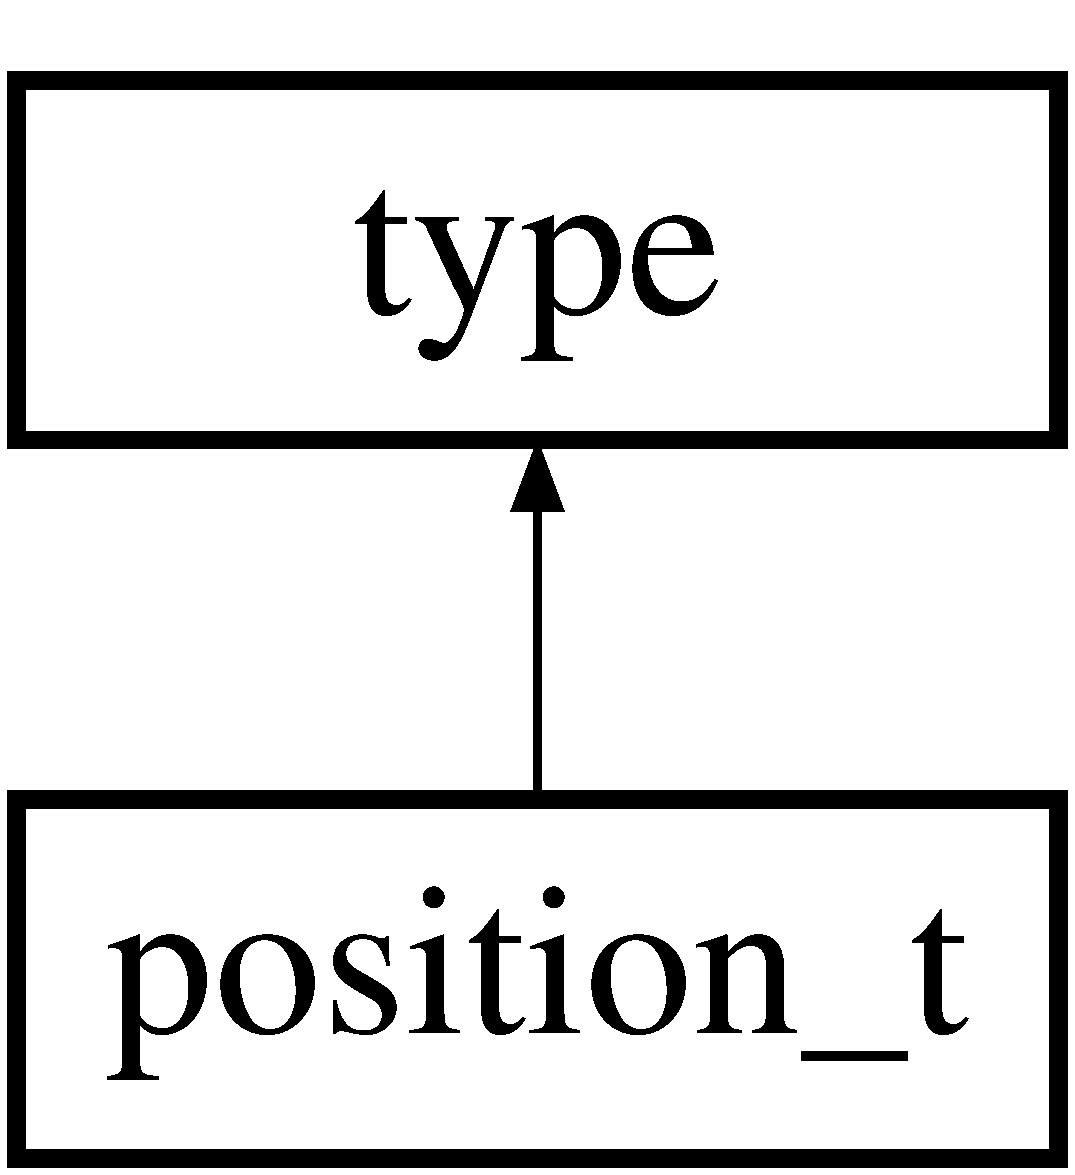
\includegraphics[height=2.000000cm]{classposition__t}
\end{center}
\end{figure}
\subsection*{Public Types}
\begin{DoxyCompactItemize}
\item 
typedef \-::\hyperlink{namespacexml__schema_a69bfaf24f63a8c18ebd8e21db6b343df}{xml\-\_\-schema\-::decimal} \hyperlink{classposition__t_a591a4bfd8546a40bc8dfca674cb54719}{x\-\_\-type}
\item 
typedef \\*
\-::xsd\-::cxx\-::tree\-::traits\\*
$<$ \hyperlink{classposition__t_a591a4bfd8546a40bc8dfca674cb54719}{x\-\_\-type}, char,\-::xsd\-::cxx\-::tree\-::schema\-\_\-type\-::decimal $>$ \hyperlink{classposition__t_a93173d63964948fabef843e84ddca444}{x\-\_\-traits}
\item 
typedef \-::\hyperlink{namespacexml__schema_a69bfaf24f63a8c18ebd8e21db6b343df}{xml\-\_\-schema\-::decimal} \hyperlink{classposition__t_afe9eaece61abab81f8ead82576de6175}{y\-\_\-type}
\item 
typedef \\*
\-::xsd\-::cxx\-::tree\-::traits\\*
$<$ \hyperlink{classposition__t_afe9eaece61abab81f8ead82576de6175}{y\-\_\-type}, char,\-::xsd\-::cxx\-::tree\-::schema\-\_\-type\-::decimal $>$ \hyperlink{classposition__t_ae9c33a2fd06ca0d9187e460c61ecb5c0}{y\-\_\-traits}
\item 
typedef \-::\hyperlink{namespacexml__schema_a69bfaf24f63a8c18ebd8e21db6b343df}{xml\-\_\-schema\-::decimal} \hyperlink{classposition__t_ab6171c246c19584481804a5e2da8561f}{z\-\_\-type}
\item 
typedef \\*
\-::xsd\-::cxx\-::tree\-::traits\\*
$<$ \hyperlink{classposition__t_ab6171c246c19584481804a5e2da8561f}{z\-\_\-type}, char,\-::xsd\-::cxx\-::tree\-::schema\-\_\-type\-::decimal $>$ \hyperlink{classposition__t_a96e8127d6eb9e048cb8f26ec77f06cd1}{z\-\_\-traits}
\end{DoxyCompactItemize}
\subsection*{Public Member Functions}
\begin{DoxyCompactItemize}
\item 
const \hyperlink{classposition__t_a591a4bfd8546a40bc8dfca674cb54719}{x\-\_\-type} \& \hyperlink{classposition__t_a3234862041a420b148df2993ed9c75b1}{x} () const 
\item 
\hyperlink{classposition__t_a591a4bfd8546a40bc8dfca674cb54719}{x\-\_\-type} \& \hyperlink{classposition__t_a258659c62b3b658406bdac021ed2a97b}{x} ()
\item 
void \hyperlink{classposition__t_a931a6a071e6849d4a1c51ae3772da0c2}{x} (const \hyperlink{classposition__t_a591a4bfd8546a40bc8dfca674cb54719}{x\-\_\-type} \&x)
\item 
const \hyperlink{classposition__t_afe9eaece61abab81f8ead82576de6175}{y\-\_\-type} \& \hyperlink{classposition__t_a44d87bd86b273e13a2dce9099a18c2f0}{y} () const 
\item 
\hyperlink{classposition__t_afe9eaece61abab81f8ead82576de6175}{y\-\_\-type} \& \hyperlink{classposition__t_ac5a4d062bbc955ef8841a4fafffede1e}{y} ()
\item 
void \hyperlink{classposition__t_a7fbc8e321a2dfa788733da0a394e76ef}{y} (const \hyperlink{classposition__t_afe9eaece61abab81f8ead82576de6175}{y\-\_\-type} \&\hyperlink{classposition__t_a3234862041a420b148df2993ed9c75b1}{x})
\item 
const \hyperlink{classposition__t_ab6171c246c19584481804a5e2da8561f}{z\-\_\-type} \& \hyperlink{classposition__t_a9bd87ff076c8148d2006032ca384f101}{z} () const 
\item 
\hyperlink{classposition__t_ab6171c246c19584481804a5e2da8561f}{z\-\_\-type} \& \hyperlink{classposition__t_acf62d9861058a8cdcb6d92b0186ceb81}{z} ()
\item 
void \hyperlink{classposition__t_a6aaf348ba089e6c78be08d551e7ff5a5}{z} (const \hyperlink{classposition__t_ab6171c246c19584481804a5e2da8561f}{z\-\_\-type} \&\hyperlink{classposition__t_a3234862041a420b148df2993ed9c75b1}{x})
\item 
\hyperlink{classposition__t_a2eba479a9a39113d71a355f87ee23a5f}{position\-\_\-t} (const \hyperlink{classposition__t_a591a4bfd8546a40bc8dfca674cb54719}{x\-\_\-type} \&, const \hyperlink{classposition__t_afe9eaece61abab81f8ead82576de6175}{y\-\_\-type} \&, const \hyperlink{classposition__t_ab6171c246c19584481804a5e2da8561f}{z\-\_\-type} \&)
\item 
\hyperlink{classposition__t_a3ca2cfedb786d6549dcc17d75ee5a8b7}{position\-\_\-t} (const \-::xercesc\-::\-D\-O\-M\-Element \&e,\-::\hyperlink{namespacexml__schema_a0612287d030cb2732d31a45b258fdc87}{xml\-\_\-schema\-::flags} f=0,\-::\hyperlink{namespacexml__schema_ada9aa30dc722e93ee2ed7243085402a5}{xml\-\_\-schema\-::container} $\ast$c=0)
\item 
\hyperlink{classposition__t_a5091933185d72e4570b86f415ff162aa}{position\-\_\-t} (const \hyperlink{classposition__t}{position\-\_\-t} \&\hyperlink{classposition__t_a3234862041a420b148df2993ed9c75b1}{x},\-::\hyperlink{namespacexml__schema_a0612287d030cb2732d31a45b258fdc87}{xml\-\_\-schema\-::flags} f=0,\-::\hyperlink{namespacexml__schema_ada9aa30dc722e93ee2ed7243085402a5}{xml\-\_\-schema\-::container} $\ast$c=0)
\item 
virtual \hyperlink{classposition__t}{position\-\_\-t} $\ast$ \hyperlink{classposition__t_adb0ccfcaf18fb57f380cc1bdbd353a82}{\-\_\-clone} (\-::\hyperlink{namespacexml__schema_a0612287d030cb2732d31a45b258fdc87}{xml\-\_\-schema\-::flags} f=0,\-::\hyperlink{namespacexml__schema_ada9aa30dc722e93ee2ed7243085402a5}{xml\-\_\-schema\-::container} $\ast$c=0) const 
\item 
virtual \hyperlink{classposition__t_a01bc521c744140617a4ee656af3e4d3a}{$\sim$position\-\_\-t} ()
\end{DoxyCompactItemize}
\subsection*{Protected Member Functions}
\begin{DoxyCompactItemize}
\item 
void \hyperlink{classposition__t_a64e519162990fff9d30d7d54c0ec48da}{parse} (\-::xsd\-::cxx\-::xml\-::dom\-::parser$<$ char $>$ \&,\-::\hyperlink{namespacexml__schema_a0612287d030cb2732d31a45b258fdc87}{xml\-\_\-schema\-::flags})
\end{DoxyCompactItemize}
\subsection*{Protected Attributes}
\begin{DoxyCompactItemize}
\item 
\-::xsd\-::cxx\-::tree\-::one$<$ \hyperlink{classposition__t_a591a4bfd8546a40bc8dfca674cb54719}{x\-\_\-type} $>$ \hyperlink{classposition__t_a60250d37007dbfaa7fa16ab2c1917db7}{x\-\_\-}
\item 
\-::xsd\-::cxx\-::tree\-::one$<$ \hyperlink{classposition__t_afe9eaece61abab81f8ead82576de6175}{y\-\_\-type} $>$ \hyperlink{classposition__t_aa907630b4c4487935e5f4f3a10835300}{y\-\_\-}
\item 
\-::xsd\-::cxx\-::tree\-::one$<$ \hyperlink{classposition__t_ab6171c246c19584481804a5e2da8561f}{z\-\_\-type} $>$ \hyperlink{classposition__t_af239aae25aff69d6f8934a737d4e4152}{z\-\_\-}
\end{DoxyCompactItemize}


\subsection{Member Typedef Documentation}
\hypertarget{classposition__t_a93173d63964948fabef843e84ddca444}{\index{position\-\_\-t@{position\-\_\-t}!x\-\_\-traits@{x\-\_\-traits}}
\index{x\-\_\-traits@{x\-\_\-traits}!position_t@{position\-\_\-t}}
\subsubsection[{x\-\_\-traits}]{\setlength{\rightskip}{0pt plus 5cm}typedef \-::xsd\-::cxx\-::tree\-::traits$<$ {\bf x\-\_\-type}, char, \-::xsd\-::cxx\-::tree\-::schema\-\_\-type\-::decimal $>$ {\bf position\-\_\-t\-::x\-\_\-traits}}}\label{classposition__t_a93173d63964948fabef843e84ddca444}
\hypertarget{classposition__t_a591a4bfd8546a40bc8dfca674cb54719}{\index{position\-\_\-t@{position\-\_\-t}!x\-\_\-type@{x\-\_\-type}}
\index{x\-\_\-type@{x\-\_\-type}!position_t@{position\-\_\-t}}
\subsubsection[{x\-\_\-type}]{\setlength{\rightskip}{0pt plus 5cm}typedef \-::{\bf xml\-\_\-schema\-::decimal} {\bf position\-\_\-t\-::x\-\_\-type}}}\label{classposition__t_a591a4bfd8546a40bc8dfca674cb54719}
\hypertarget{classposition__t_ae9c33a2fd06ca0d9187e460c61ecb5c0}{\index{position\-\_\-t@{position\-\_\-t}!y\-\_\-traits@{y\-\_\-traits}}
\index{y\-\_\-traits@{y\-\_\-traits}!position_t@{position\-\_\-t}}
\subsubsection[{y\-\_\-traits}]{\setlength{\rightskip}{0pt plus 5cm}typedef \-::xsd\-::cxx\-::tree\-::traits$<$ {\bf y\-\_\-type}, char, \-::xsd\-::cxx\-::tree\-::schema\-\_\-type\-::decimal $>$ {\bf position\-\_\-t\-::y\-\_\-traits}}}\label{classposition__t_ae9c33a2fd06ca0d9187e460c61ecb5c0}
\hypertarget{classposition__t_afe9eaece61abab81f8ead82576de6175}{\index{position\-\_\-t@{position\-\_\-t}!y\-\_\-type@{y\-\_\-type}}
\index{y\-\_\-type@{y\-\_\-type}!position_t@{position\-\_\-t}}
\subsubsection[{y\-\_\-type}]{\setlength{\rightskip}{0pt plus 5cm}typedef \-::{\bf xml\-\_\-schema\-::decimal} {\bf position\-\_\-t\-::y\-\_\-type}}}\label{classposition__t_afe9eaece61abab81f8ead82576de6175}
\hypertarget{classposition__t_a96e8127d6eb9e048cb8f26ec77f06cd1}{\index{position\-\_\-t@{position\-\_\-t}!z\-\_\-traits@{z\-\_\-traits}}
\index{z\-\_\-traits@{z\-\_\-traits}!position_t@{position\-\_\-t}}
\subsubsection[{z\-\_\-traits}]{\setlength{\rightskip}{0pt plus 5cm}typedef \-::xsd\-::cxx\-::tree\-::traits$<$ {\bf z\-\_\-type}, char, \-::xsd\-::cxx\-::tree\-::schema\-\_\-type\-::decimal $>$ {\bf position\-\_\-t\-::z\-\_\-traits}}}\label{classposition__t_a96e8127d6eb9e048cb8f26ec77f06cd1}
\hypertarget{classposition__t_ab6171c246c19584481804a5e2da8561f}{\index{position\-\_\-t@{position\-\_\-t}!z\-\_\-type@{z\-\_\-type}}
\index{z\-\_\-type@{z\-\_\-type}!position_t@{position\-\_\-t}}
\subsubsection[{z\-\_\-type}]{\setlength{\rightskip}{0pt plus 5cm}typedef \-::{\bf xml\-\_\-schema\-::decimal} {\bf position\-\_\-t\-::z\-\_\-type}}}\label{classposition__t_ab6171c246c19584481804a5e2da8561f}


\subsection{Constructor \& Destructor Documentation}
\hypertarget{classposition__t_a2eba479a9a39113d71a355f87ee23a5f}{\index{position\-\_\-t@{position\-\_\-t}!position\-\_\-t@{position\-\_\-t}}
\index{position\-\_\-t@{position\-\_\-t}!position_t@{position\-\_\-t}}
\subsubsection[{position\-\_\-t}]{\setlength{\rightskip}{0pt plus 5cm}position\-\_\-t\-::position\-\_\-t (
\begin{DoxyParamCaption}
\item[{const {\bf x\-\_\-type} \&}]{x, }
\item[{const {\bf y\-\_\-type} \&}]{y, }
\item[{const {\bf z\-\_\-type} \&}]{z}
\end{DoxyParamCaption}
)}}\label{classposition__t_a2eba479a9a39113d71a355f87ee23a5f}
\hypertarget{classposition__t_a3ca2cfedb786d6549dcc17d75ee5a8b7}{\index{position\-\_\-t@{position\-\_\-t}!position\-\_\-t@{position\-\_\-t}}
\index{position\-\_\-t@{position\-\_\-t}!position_t@{position\-\_\-t}}
\subsubsection[{position\-\_\-t}]{\setlength{\rightskip}{0pt plus 5cm}position\-\_\-t\-::position\-\_\-t (
\begin{DoxyParamCaption}
\item[{const \-::xercesc\-::\-D\-O\-M\-Element \&}]{e, }
\item[{\-::{\bf xml\-\_\-schema\-::flags}}]{f = {\ttfamily 0}, }
\item[{\-::{\bf xml\-\_\-schema\-::container} $\ast$}]{c = {\ttfamily 0}}
\end{DoxyParamCaption}
)}}\label{classposition__t_a3ca2cfedb786d6549dcc17d75ee5a8b7}
\hypertarget{classposition__t_a5091933185d72e4570b86f415ff162aa}{\index{position\-\_\-t@{position\-\_\-t}!position\-\_\-t@{position\-\_\-t}}
\index{position\-\_\-t@{position\-\_\-t}!position_t@{position\-\_\-t}}
\subsubsection[{position\-\_\-t}]{\setlength{\rightskip}{0pt plus 5cm}position\-\_\-t\-::position\-\_\-t (
\begin{DoxyParamCaption}
\item[{const {\bf position\-\_\-t} \&}]{x, }
\item[{\-::{\bf xml\-\_\-schema\-::flags}}]{f = {\ttfamily 0}, }
\item[{\-::{\bf xml\-\_\-schema\-::container} $\ast$}]{c = {\ttfamily 0}}
\end{DoxyParamCaption}
)}}\label{classposition__t_a5091933185d72e4570b86f415ff162aa}
\hypertarget{classposition__t_a01bc521c744140617a4ee656af3e4d3a}{\index{position\-\_\-t@{position\-\_\-t}!$\sim$position\-\_\-t@{$\sim$position\-\_\-t}}
\index{$\sim$position\-\_\-t@{$\sim$position\-\_\-t}!position_t@{position\-\_\-t}}
\subsubsection[{$\sim$position\-\_\-t}]{\setlength{\rightskip}{0pt plus 5cm}position\-\_\-t\-::$\sim$position\-\_\-t (
\begin{DoxyParamCaption}
{}
\end{DoxyParamCaption}
)\hspace{0.3cm}{\ttfamily [virtual]}}}\label{classposition__t_a01bc521c744140617a4ee656af3e4d3a}


\subsection{Member Function Documentation}
\hypertarget{classposition__t_adb0ccfcaf18fb57f380cc1bdbd353a82}{\index{position\-\_\-t@{position\-\_\-t}!\-\_\-clone@{\-\_\-clone}}
\index{\-\_\-clone@{\-\_\-clone}!position_t@{position\-\_\-t}}
\subsubsection[{\-\_\-clone}]{\setlength{\rightskip}{0pt plus 5cm}{\bf position\-\_\-t} $\ast$ position\-\_\-t\-::\-\_\-clone (
\begin{DoxyParamCaption}
\item[{\-::{\bf xml\-\_\-schema\-::flags}}]{f = {\ttfamily 0}, }
\item[{\-::{\bf xml\-\_\-schema\-::container} $\ast$}]{c = {\ttfamily 0}}
\end{DoxyParamCaption}
) const\hspace{0.3cm}{\ttfamily [virtual]}}}\label{classposition__t_adb0ccfcaf18fb57f380cc1bdbd353a82}
\hypertarget{classposition__t_a64e519162990fff9d30d7d54c0ec48da}{\index{position\-\_\-t@{position\-\_\-t}!parse@{parse}}
\index{parse@{parse}!position_t@{position\-\_\-t}}
\subsubsection[{parse}]{\setlength{\rightskip}{0pt plus 5cm}void position\-\_\-t\-::parse (
\begin{DoxyParamCaption}
\item[{\-::xsd\-::cxx\-::xml\-::dom\-::parser$<$ char $>$ \&}]{p, }
\item[{\-::{\bf xml\-\_\-schema\-::flags}}]{f}
\end{DoxyParamCaption}
)\hspace{0.3cm}{\ttfamily [protected]}}}\label{classposition__t_a64e519162990fff9d30d7d54c0ec48da}
\hypertarget{classposition__t_a3234862041a420b148df2993ed9c75b1}{\index{position\-\_\-t@{position\-\_\-t}!x@{x}}
\index{x@{x}!position_t@{position\-\_\-t}}
\subsubsection[{x}]{\setlength{\rightskip}{0pt plus 5cm}const {\bf position\-\_\-t\-::x\-\_\-type} \& position\-\_\-t\-::x (
\begin{DoxyParamCaption}
{}
\end{DoxyParamCaption}
) const}}\label{classposition__t_a3234862041a420b148df2993ed9c75b1}
\hypertarget{classposition__t_a258659c62b3b658406bdac021ed2a97b}{\index{position\-\_\-t@{position\-\_\-t}!x@{x}}
\index{x@{x}!position_t@{position\-\_\-t}}
\subsubsection[{x}]{\setlength{\rightskip}{0pt plus 5cm}{\bf position\-\_\-t\-::x\-\_\-type} \& position\-\_\-t\-::x (
\begin{DoxyParamCaption}
{}
\end{DoxyParamCaption}
)}}\label{classposition__t_a258659c62b3b658406bdac021ed2a97b}
\hypertarget{classposition__t_a931a6a071e6849d4a1c51ae3772da0c2}{\index{position\-\_\-t@{position\-\_\-t}!x@{x}}
\index{x@{x}!position_t@{position\-\_\-t}}
\subsubsection[{x}]{\setlength{\rightskip}{0pt plus 5cm}void position\-\_\-t\-::x (
\begin{DoxyParamCaption}
\item[{const {\bf x\-\_\-type} \&}]{x}
\end{DoxyParamCaption}
)}}\label{classposition__t_a931a6a071e6849d4a1c51ae3772da0c2}
\hypertarget{classposition__t_a44d87bd86b273e13a2dce9099a18c2f0}{\index{position\-\_\-t@{position\-\_\-t}!y@{y}}
\index{y@{y}!position_t@{position\-\_\-t}}
\subsubsection[{y}]{\setlength{\rightskip}{0pt plus 5cm}const {\bf position\-\_\-t\-::y\-\_\-type} \& position\-\_\-t\-::y (
\begin{DoxyParamCaption}
{}
\end{DoxyParamCaption}
) const}}\label{classposition__t_a44d87bd86b273e13a2dce9099a18c2f0}
\hypertarget{classposition__t_ac5a4d062bbc955ef8841a4fafffede1e}{\index{position\-\_\-t@{position\-\_\-t}!y@{y}}
\index{y@{y}!position_t@{position\-\_\-t}}
\subsubsection[{y}]{\setlength{\rightskip}{0pt plus 5cm}{\bf position\-\_\-t\-::y\-\_\-type} \& position\-\_\-t\-::y (
\begin{DoxyParamCaption}
{}
\end{DoxyParamCaption}
)}}\label{classposition__t_ac5a4d062bbc955ef8841a4fafffede1e}
\hypertarget{classposition__t_a7fbc8e321a2dfa788733da0a394e76ef}{\index{position\-\_\-t@{position\-\_\-t}!y@{y}}
\index{y@{y}!position_t@{position\-\_\-t}}
\subsubsection[{y}]{\setlength{\rightskip}{0pt plus 5cm}void position\-\_\-t\-::y (
\begin{DoxyParamCaption}
\item[{const {\bf y\-\_\-type} \&}]{x}
\end{DoxyParamCaption}
)}}\label{classposition__t_a7fbc8e321a2dfa788733da0a394e76ef}
\hypertarget{classposition__t_a9bd87ff076c8148d2006032ca384f101}{\index{position\-\_\-t@{position\-\_\-t}!z@{z}}
\index{z@{z}!position_t@{position\-\_\-t}}
\subsubsection[{z}]{\setlength{\rightskip}{0pt plus 5cm}const {\bf position\-\_\-t\-::z\-\_\-type} \& position\-\_\-t\-::z (
\begin{DoxyParamCaption}
{}
\end{DoxyParamCaption}
) const}}\label{classposition__t_a9bd87ff076c8148d2006032ca384f101}
\hypertarget{classposition__t_acf62d9861058a8cdcb6d92b0186ceb81}{\index{position\-\_\-t@{position\-\_\-t}!z@{z}}
\index{z@{z}!position_t@{position\-\_\-t}}
\subsubsection[{z}]{\setlength{\rightskip}{0pt plus 5cm}{\bf position\-\_\-t\-::z\-\_\-type} \& position\-\_\-t\-::z (
\begin{DoxyParamCaption}
{}
\end{DoxyParamCaption}
)}}\label{classposition__t_acf62d9861058a8cdcb6d92b0186ceb81}
\hypertarget{classposition__t_a6aaf348ba089e6c78be08d551e7ff5a5}{\index{position\-\_\-t@{position\-\_\-t}!z@{z}}
\index{z@{z}!position_t@{position\-\_\-t}}
\subsubsection[{z}]{\setlength{\rightskip}{0pt plus 5cm}void position\-\_\-t\-::z (
\begin{DoxyParamCaption}
\item[{const {\bf z\-\_\-type} \&}]{x}
\end{DoxyParamCaption}
)}}\label{classposition__t_a6aaf348ba089e6c78be08d551e7ff5a5}


\subsection{Member Data Documentation}
\hypertarget{classposition__t_a60250d37007dbfaa7fa16ab2c1917db7}{\index{position\-\_\-t@{position\-\_\-t}!x\-\_\-@{x\-\_\-}}
\index{x\-\_\-@{x\-\_\-}!position_t@{position\-\_\-t}}
\subsubsection[{x\-\_\-}]{\setlength{\rightskip}{0pt plus 5cm}\-::xsd\-::cxx\-::tree\-::one$<$ {\bf x\-\_\-type} $>$ position\-\_\-t\-::x\-\_\-\hspace{0.3cm}{\ttfamily [protected]}}}\label{classposition__t_a60250d37007dbfaa7fa16ab2c1917db7}
\hypertarget{classposition__t_aa907630b4c4487935e5f4f3a10835300}{\index{position\-\_\-t@{position\-\_\-t}!y\-\_\-@{y\-\_\-}}
\index{y\-\_\-@{y\-\_\-}!position_t@{position\-\_\-t}}
\subsubsection[{y\-\_\-}]{\setlength{\rightskip}{0pt plus 5cm}\-::xsd\-::cxx\-::tree\-::one$<$ {\bf y\-\_\-type} $>$ position\-\_\-t\-::y\-\_\-\hspace{0.3cm}{\ttfamily [protected]}}}\label{classposition__t_aa907630b4c4487935e5f4f3a10835300}
\hypertarget{classposition__t_af239aae25aff69d6f8934a737d4e4152}{\index{position\-\_\-t@{position\-\_\-t}!z\-\_\-@{z\-\_\-}}
\index{z\-\_\-@{z\-\_\-}!position_t@{position\-\_\-t}}
\subsubsection[{z\-\_\-}]{\setlength{\rightskip}{0pt plus 5cm}\-::xsd\-::cxx\-::tree\-::one$<$ {\bf z\-\_\-type} $>$ position\-\_\-t\-::z\-\_\-\hspace{0.3cm}{\ttfamily [protected]}}}\label{classposition__t_af239aae25aff69d6f8934a737d4e4152}


The documentation for this class was generated from the following files\-:\begin{DoxyCompactItemize}
\item 
src/utils/\hyperlink{InputParticles_8h}{Input\-Particles.\-h}\item 
src/utils/\hyperlink{InputParticles_8cpp}{Input\-Particles.\-cpp}\end{DoxyCompactItemize}

\hypertarget{classpse__t}{\section{pse\-\_\-t Class Reference}
\label{classpse__t}\index{pse\-\_\-t@{pse\-\_\-t}}
}


{\ttfamily \#include $<$Input\-Setting.\-h$>$}

Inheritance diagram for pse\-\_\-t\-:\begin{figure}[H]
\begin{center}
\leavevmode
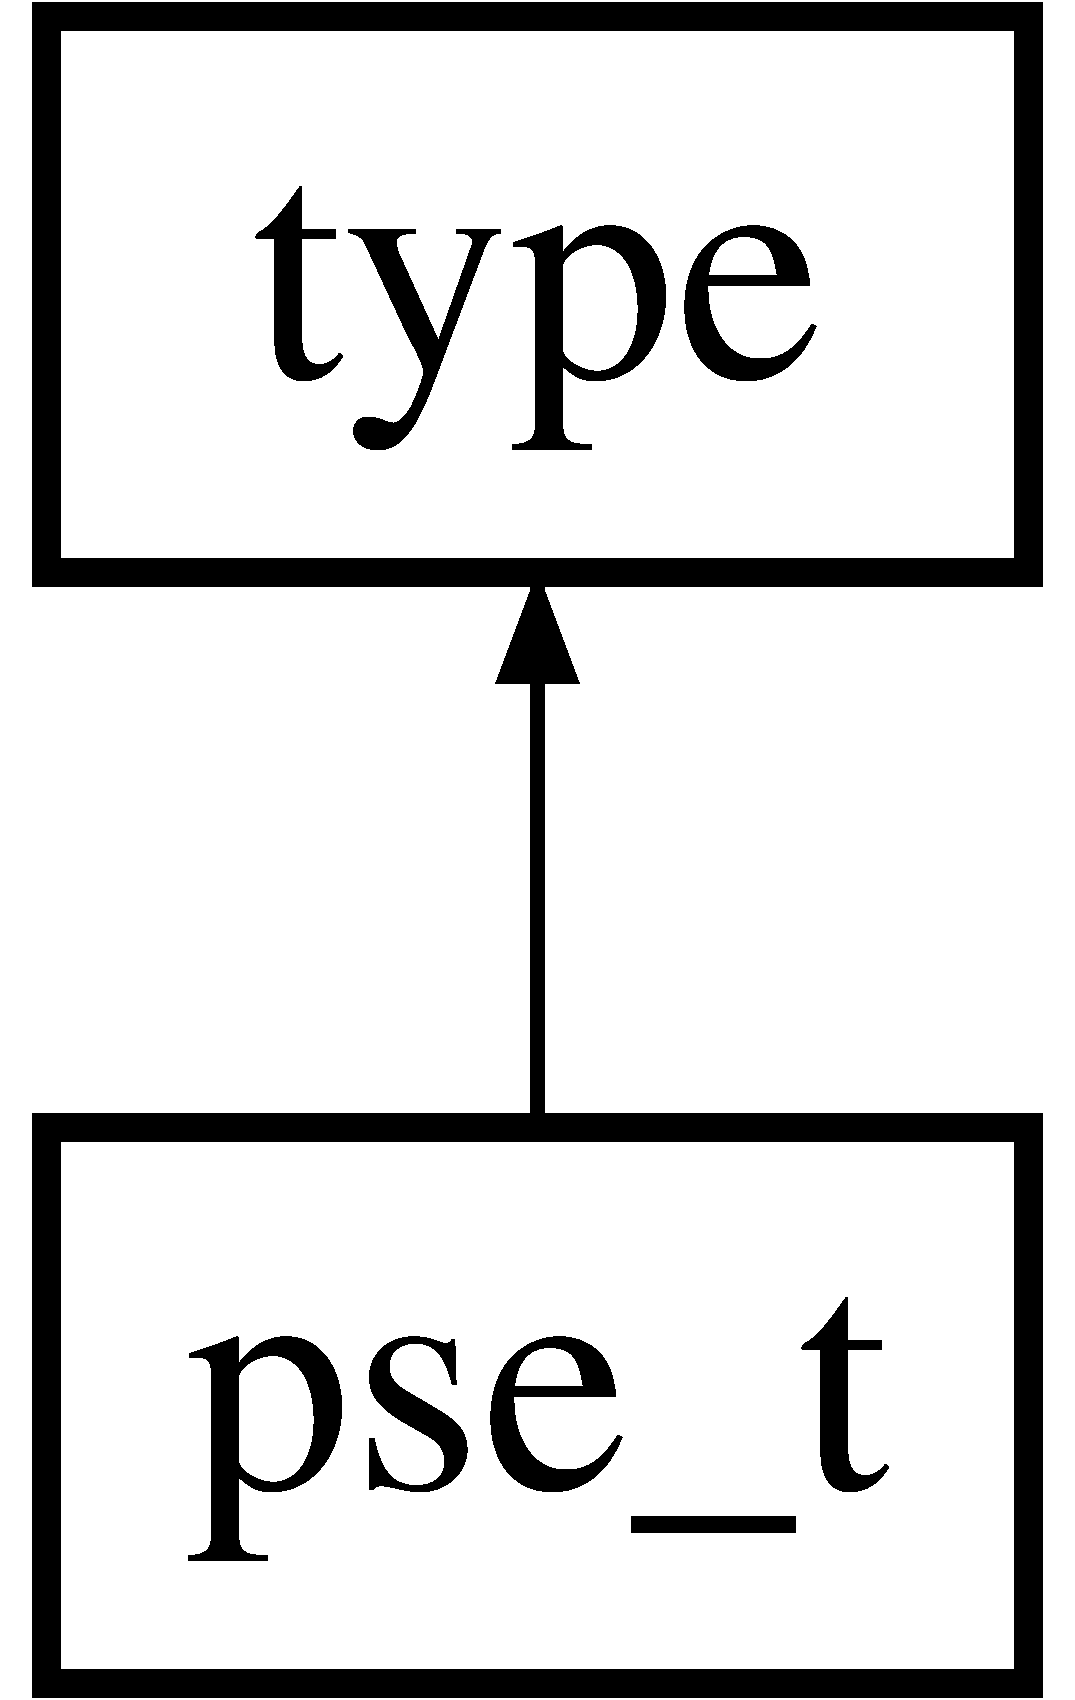
\includegraphics[height=2.000000cm]{classpse__t}
\end{center}
\end{figure}
\subsection*{Public Types}
\begin{DoxyCompactItemize}
\item 
typedef \-::\hyperlink{namespacexml__schema_a69bfaf24f63a8c18ebd8e21db6b343df}{xml\-\_\-schema\-::decimal} \hyperlink{classpse__t_a2b49c9d348499d75809e2b655582eb6f}{start\-\_\-time\-\_\-type}
\item 
typedef \\*
\-::xsd\-::cxx\-::tree\-::traits\\*
$<$ \hyperlink{classpse__t_a2b49c9d348499d75809e2b655582eb6f}{start\-\_\-time\-\_\-type}, char,\-::xsd\-::cxx\-::tree\-::schema\-\_\-type\-::decimal $>$ \hyperlink{classpse__t_ab28e5b3d2a24ea5a9b120b25dd1a27ac}{start\-\_\-time\-\_\-traits}
\item 
typedef \-::\hyperlink{namespacexml__schema_a69bfaf24f63a8c18ebd8e21db6b343df}{xml\-\_\-schema\-::decimal} \hyperlink{classpse__t_ac4239e9fa324e53f5964848e3089fef6}{t\-\_\-end\-\_\-type}
\item 
typedef \\*
\-::xsd\-::cxx\-::tree\-::traits\\*
$<$ \hyperlink{classpse__t_ac4239e9fa324e53f5964848e3089fef6}{t\-\_\-end\-\_\-type}, char,\-::xsd\-::cxx\-::tree\-::schema\-\_\-type\-::decimal $>$ \hyperlink{classpse__t_a4de32dd1347fe5653d7b6f581929e3ba}{t\-\_\-end\-\_\-traits}
\item 
typedef \-::\hyperlink{namespacexml__schema_a69bfaf24f63a8c18ebd8e21db6b343df}{xml\-\_\-schema\-::decimal} \hyperlink{classpse__t_a7af94a081ff80545fa4d069c4ba56b57}{delta\-\_\-t\-\_\-type}
\item 
typedef \\*
\-::xsd\-::cxx\-::tree\-::traits\\*
$<$ \hyperlink{classpse__t_a7af94a081ff80545fa4d069c4ba56b57}{delta\-\_\-t\-\_\-type}, char,\-::xsd\-::cxx\-::tree\-::schema\-\_\-type\-::decimal $>$ \hyperlink{classpse__t_a02b088d0313bad0fedf219ccf44ebe48}{delta\-\_\-t\-\_\-traits}
\item 
typedef \-::\hyperlink{namespacexml__schema_acfa24ac68e1a188e7f44c36f7a158bf4}{xml\-\_\-schema\-::int\-\_\-} \hyperlink{classpse__t_a3aa6a8cc1b9642304371fb935f6e1965}{number\-Of\-Types\-\_\-type}
\item 
typedef \\*
\-::xsd\-::cxx\-::tree\-::traits\\*
$<$ \hyperlink{classpse__t_a3aa6a8cc1b9642304371fb935f6e1965}{number\-Of\-Types\-\_\-type}, char $>$ \hyperlink{classpse__t_af86f3cfbbdef30f8a4a5927642e947bf}{number\-Of\-Types\-\_\-traits}
\item 
typedef \-::\hyperlink{namespacexml__schema_a69bfaf24f63a8c18ebd8e21db6b343df}{xml\-\_\-schema\-::decimal} \hyperlink{classpse__t_a86b52d56dfb0c43a023d8bda8b4a19ed}{gconst\-\_\-type}
\item 
typedef \\*
\-::xsd\-::cxx\-::tree\-::traits\\*
$<$ \hyperlink{classpse__t_a86b52d56dfb0c43a023d8bda8b4a19ed}{gconst\-\_\-type}, char,\-::xsd\-::cxx\-::tree\-::schema\-\_\-type\-::decimal $>$ \hyperlink{classpse__t_a9074dfb701a5e94c508dda07a4afe61b}{gconst\-\_\-traits}
\item 
typedef \-::\hyperlink{classlc__t}{lc\-\_\-t} \hyperlink{classpse__t_aa6a9bda12a405c1b9fb0baecbed9a1bb}{lc\-\_\-type}
\item 
typedef \\*
\-::xsd\-::cxx\-::tree\-::traits\\*
$<$ \hyperlink{classpse__t_aa6a9bda12a405c1b9fb0baecbed9a1bb}{lc\-\_\-type}, char $>$ \hyperlink{classpse__t_a3e552e037801ee7f00dbfb46a0a860f6}{lc\-\_\-traits}
\item 
typedef \-::\hyperlink{classthermo__t}{thermo\-\_\-t} \hyperlink{classpse__t_aebaae32f697fb451e7bab83078867d4e}{thermo\-\_\-type}
\item 
typedef \\*
\-::xsd\-::cxx\-::tree\-::traits\\*
$<$ \hyperlink{classpse__t_aebaae32f697fb451e7bab83078867d4e}{thermo\-\_\-type}, char $>$ \hyperlink{classpse__t_a3c730d4487efb386ba2d36da2bd1dbd0}{thermo\-\_\-traits}
\item 
typedef \-::\hyperlink{classinputfile__t}{inputfile\-\_\-t} \hyperlink{classpse__t_a86a1a849175762d6b2d8d254a694d43c}{inputfile\-\_\-type}
\item 
typedef \\*
\-::xsd\-::cxx\-::tree\-::sequence\\*
$<$ \hyperlink{classpse__t_a86a1a849175762d6b2d8d254a694d43c}{inputfile\-\_\-type} $>$ \hyperlink{classpse__t_a4256607256aa600165964a3a6d7b4a00}{inputfile\-\_\-sequence}
\item 
typedef \\*
inputfile\-\_\-sequence\-::iterator \hyperlink{classpse__t_a18cbe2015326033fa7dc6f53112daa5f}{inputfile\-\_\-iterator}
\item 
typedef \\*
inputfile\-\_\-sequence\-::const\-\_\-iterator \hyperlink{classpse__t_a56e96d807f4fb19912690b53fe95d20b}{inputfile\-\_\-const\-\_\-iterator}
\item 
typedef \\*
\-::xsd\-::cxx\-::tree\-::traits\\*
$<$ \hyperlink{classpse__t_a86a1a849175762d6b2d8d254a694d43c}{inputfile\-\_\-type}, char $>$ \hyperlink{classpse__t_aa1b26e25c5698d3db17f0d9997faec05}{inputfile\-\_\-traits}
\item 
typedef \-::\hyperlink{classoutputfile__t}{outputfile\-\_\-t} \hyperlink{classpse__t_ae86d42dbfdd42a4d53733b6b11b5f875}{outputfile\-\_\-type}
\item 
typedef \\*
\-::xsd\-::cxx\-::tree\-::traits\\*
$<$ \hyperlink{classpse__t_ae86d42dbfdd42a4d53733b6b11b5f875}{outputfile\-\_\-type}, char $>$ \hyperlink{classpse__t_a1ea902d4f686908c24a487b7a16fcb0a}{outputfile\-\_\-traits}
\end{DoxyCompactItemize}
\subsection*{Public Member Functions}
\begin{DoxyCompactItemize}
\item 
const \hyperlink{classpse__t_a2b49c9d348499d75809e2b655582eb6f}{start\-\_\-time\-\_\-type} \& \hyperlink{classpse__t_a28a55f99317bef129c37b03bf9dca7a3}{start\-\_\-time} () const 
\item 
\hyperlink{classpse__t_a2b49c9d348499d75809e2b655582eb6f}{start\-\_\-time\-\_\-type} \& \hyperlink{classpse__t_acac91424c4b53e6cf03f7730d2fdfc4e}{start\-\_\-time} ()
\item 
void \hyperlink{classpse__t_a0f2ad06174e2c781909ac48facf7ef10}{start\-\_\-time} (const \hyperlink{classpse__t_a2b49c9d348499d75809e2b655582eb6f}{start\-\_\-time\-\_\-type} \&x)
\item 
const \hyperlink{classpse__t_ac4239e9fa324e53f5964848e3089fef6}{t\-\_\-end\-\_\-type} \& \hyperlink{classpse__t_ad6ff0c1f53ea1b2aead01da2b10e67fa}{t\-\_\-end} () const 
\item 
\hyperlink{classpse__t_ac4239e9fa324e53f5964848e3089fef6}{t\-\_\-end\-\_\-type} \& \hyperlink{classpse__t_afe6617147ae653198a203a3cf1969789}{t\-\_\-end} ()
\item 
void \hyperlink{classpse__t_a6fe90c1ea798d2a805953d2b74c94050}{t\-\_\-end} (const \hyperlink{classpse__t_ac4239e9fa324e53f5964848e3089fef6}{t\-\_\-end\-\_\-type} \&x)
\item 
const \hyperlink{classpse__t_a7af94a081ff80545fa4d069c4ba56b57}{delta\-\_\-t\-\_\-type} \& \hyperlink{classpse__t_a295fda39af32ccb4903c2589c431d56a}{delta\-\_\-t} () const 
\item 
\hyperlink{classpse__t_a7af94a081ff80545fa4d069c4ba56b57}{delta\-\_\-t\-\_\-type} \& \hyperlink{classpse__t_af963897076ecce82a7cfa4e739a2c821}{delta\-\_\-t} ()
\item 
void \hyperlink{classpse__t_ab5ab165c9d30017fb0cde2b3e55c816a}{delta\-\_\-t} (const \hyperlink{classpse__t_a7af94a081ff80545fa4d069c4ba56b57}{delta\-\_\-t\-\_\-type} \&x)
\item 
const \hyperlink{classpse__t_a3aa6a8cc1b9642304371fb935f6e1965}{number\-Of\-Types\-\_\-type} \& \hyperlink{classpse__t_a26abadfd643121531b460870d6b44dbe}{number\-Of\-Types} () const 
\item 
\hyperlink{classpse__t_a3aa6a8cc1b9642304371fb935f6e1965}{number\-Of\-Types\-\_\-type} \& \hyperlink{classpse__t_a10db3efbceafc329141c4b0e6205f200}{number\-Of\-Types} ()
\item 
void \hyperlink{classpse__t_afc33f5fb9ec3a56d45965b492f1c2c74}{number\-Of\-Types} (const \hyperlink{classpse__t_a3aa6a8cc1b9642304371fb935f6e1965}{number\-Of\-Types\-\_\-type} \&x)
\item 
const \hyperlink{classpse__t_a86b52d56dfb0c43a023d8bda8b4a19ed}{gconst\-\_\-type} \& \hyperlink{classpse__t_a56275a79bb5be350e896bdb8f96e9d0f}{gconst} () const 
\item 
\hyperlink{classpse__t_a86b52d56dfb0c43a023d8bda8b4a19ed}{gconst\-\_\-type} \& \hyperlink{classpse__t_a015cbd6cae33a2cbac8dfe6de45fc21b}{gconst} ()
\item 
void \hyperlink{classpse__t_af993fd9228e70d7fd21d5e29f296c6d9}{gconst} (const \hyperlink{classpse__t_a86b52d56dfb0c43a023d8bda8b4a19ed}{gconst\-\_\-type} \&x)
\item 
const \hyperlink{classpse__t_aa6a9bda12a405c1b9fb0baecbed9a1bb}{lc\-\_\-type} \& \hyperlink{classpse__t_a655f53f51144ada990e701b11a774553}{lc} () const 
\item 
\hyperlink{classpse__t_aa6a9bda12a405c1b9fb0baecbed9a1bb}{lc\-\_\-type} \& \hyperlink{classpse__t_afe44e5cd915052e6f62606e3401715e8}{lc} ()
\item 
void \hyperlink{classpse__t_ab0cd9346111c00b628bf7c204f7b76f8}{lc} (const \hyperlink{classpse__t_aa6a9bda12a405c1b9fb0baecbed9a1bb}{lc\-\_\-type} \&x)
\item 
void \hyperlink{classpse__t_a2745fd4372fa60a11ac7e2a28ef9da58}{lc} (\-::std\-::auto\-\_\-ptr$<$ \hyperlink{classpse__t_aa6a9bda12a405c1b9fb0baecbed9a1bb}{lc\-\_\-type} $>$ p)
\item 
const \hyperlink{classpse__t_aebaae32f697fb451e7bab83078867d4e}{thermo\-\_\-type} \& \hyperlink{classpse__t_abb2d165dc54a3477fc981c259b62ace8}{thermo} () const 
\item 
\hyperlink{classpse__t_aebaae32f697fb451e7bab83078867d4e}{thermo\-\_\-type} \& \hyperlink{classpse__t_a2c201aa23372362451be0eed3399b4fc}{thermo} ()
\item 
void \hyperlink{classpse__t_a7c4f6a3d067fc6263d33c66306d5fb46}{thermo} (const \hyperlink{classpse__t_aebaae32f697fb451e7bab83078867d4e}{thermo\-\_\-type} \&x)
\item 
void \hyperlink{classpse__t_a223df3e0d39422c4bc43a573972373a4}{thermo} (\-::std\-::auto\-\_\-ptr$<$ \hyperlink{classpse__t_aebaae32f697fb451e7bab83078867d4e}{thermo\-\_\-type} $>$ p)
\item 
const \hyperlink{classpse__t_a4256607256aa600165964a3a6d7b4a00}{inputfile\-\_\-sequence} \& \hyperlink{classpse__t_aaedba73e5a7e32a7c8a09dcb53e888ac}{inputfile} () const 
\item 
\hyperlink{classpse__t_a4256607256aa600165964a3a6d7b4a00}{inputfile\-\_\-sequence} \& \hyperlink{classpse__t_ab2ad9a71f6a781c2e7fcbe42a708cd7c}{inputfile} ()
\item 
void \hyperlink{classpse__t_acf62869d9c38c6b59cb858bd82433ebc}{inputfile} (const \hyperlink{classpse__t_a4256607256aa600165964a3a6d7b4a00}{inputfile\-\_\-sequence} \&s)
\item 
const \hyperlink{classpse__t_ae86d42dbfdd42a4d53733b6b11b5f875}{outputfile\-\_\-type} \& \hyperlink{classpse__t_a422c3cc4009f845d32b4246ff34e7507}{outputfile} () const 
\item 
\hyperlink{classpse__t_ae86d42dbfdd42a4d53733b6b11b5f875}{outputfile\-\_\-type} \& \hyperlink{classpse__t_a51b629a444eb46dead05e358217580fa}{outputfile} ()
\item 
void \hyperlink{classpse__t_a9820d2ff1eb7021c87507b5dbe97569f}{outputfile} (const \hyperlink{classpse__t_ae86d42dbfdd42a4d53733b6b11b5f875}{outputfile\-\_\-type} \&x)
\item 
void \hyperlink{classpse__t_a57dce4a2d7e11de9c53dd050ca3a02ae}{outputfile} (\-::std\-::auto\-\_\-ptr$<$ \hyperlink{classpse__t_ae86d42dbfdd42a4d53733b6b11b5f875}{outputfile\-\_\-type} $>$ p)
\item 
\hyperlink{classpse__t_abf13db7637cd0458dd528641e5c0236d}{pse\-\_\-t} (const \hyperlink{classpse__t_a2b49c9d348499d75809e2b655582eb6f}{start\-\_\-time\-\_\-type} \&, const \hyperlink{classpse__t_ac4239e9fa324e53f5964848e3089fef6}{t\-\_\-end\-\_\-type} \&, const \hyperlink{classpse__t_a7af94a081ff80545fa4d069c4ba56b57}{delta\-\_\-t\-\_\-type} \&, const \hyperlink{classpse__t_a3aa6a8cc1b9642304371fb935f6e1965}{number\-Of\-Types\-\_\-type} \&, const \hyperlink{classpse__t_a86b52d56dfb0c43a023d8bda8b4a19ed}{gconst\-\_\-type} \&, const \hyperlink{classpse__t_aa6a9bda12a405c1b9fb0baecbed9a1bb}{lc\-\_\-type} \&, const \hyperlink{classpse__t_aebaae32f697fb451e7bab83078867d4e}{thermo\-\_\-type} \&, const \hyperlink{classpse__t_ae86d42dbfdd42a4d53733b6b11b5f875}{outputfile\-\_\-type} \&)
\item 
\hyperlink{classpse__t_a5a5effaf61883042a01c631c2cd32aee}{pse\-\_\-t} (const \hyperlink{classpse__t_a2b49c9d348499d75809e2b655582eb6f}{start\-\_\-time\-\_\-type} \&, const \hyperlink{classpse__t_ac4239e9fa324e53f5964848e3089fef6}{t\-\_\-end\-\_\-type} \&, const \hyperlink{classpse__t_a7af94a081ff80545fa4d069c4ba56b57}{delta\-\_\-t\-\_\-type} \&, const \hyperlink{classpse__t_a3aa6a8cc1b9642304371fb935f6e1965}{number\-Of\-Types\-\_\-type} \&, const \hyperlink{classpse__t_a86b52d56dfb0c43a023d8bda8b4a19ed}{gconst\-\_\-type} \&,\-::std\-::auto\-\_\-ptr$<$ \hyperlink{classpse__t_aa6a9bda12a405c1b9fb0baecbed9a1bb}{lc\-\_\-type} $>$ \&,\-::std\-::auto\-\_\-ptr$<$ \hyperlink{classpse__t_aebaae32f697fb451e7bab83078867d4e}{thermo\-\_\-type} $>$ \&,\-::std\-::auto\-\_\-ptr$<$ \hyperlink{classpse__t_ae86d42dbfdd42a4d53733b6b11b5f875}{outputfile\-\_\-type} $>$ \&)
\item 
\hyperlink{classpse__t_a751d788755e53441737f792453d665a2}{pse\-\_\-t} (const \-::xercesc\-::\-D\-O\-M\-Element \&e,\-::\hyperlink{namespacexml__schema_a0612287d030cb2732d31a45b258fdc87}{xml\-\_\-schema\-::flags} f=0,\-::\hyperlink{namespacexml__schema_ada9aa30dc722e93ee2ed7243085402a5}{xml\-\_\-schema\-::container} $\ast$c=0)
\item 
\hyperlink{classpse__t_adb96d77efda033d89be5625ebfd809ae}{pse\-\_\-t} (const \hyperlink{classpse__t}{pse\-\_\-t} \&x,\-::\hyperlink{namespacexml__schema_a0612287d030cb2732d31a45b258fdc87}{xml\-\_\-schema\-::flags} f=0,\-::\hyperlink{namespacexml__schema_ada9aa30dc722e93ee2ed7243085402a5}{xml\-\_\-schema\-::container} $\ast$c=0)
\item 
virtual \hyperlink{classpse__t}{pse\-\_\-t} $\ast$ \hyperlink{classpse__t_abd24942c0ca4e9438281311fd2d80515}{\-\_\-clone} (\-::\hyperlink{namespacexml__schema_a0612287d030cb2732d31a45b258fdc87}{xml\-\_\-schema\-::flags} f=0,\-::\hyperlink{namespacexml__schema_ada9aa30dc722e93ee2ed7243085402a5}{xml\-\_\-schema\-::container} $\ast$c=0) const 
\item 
virtual \hyperlink{classpse__t_a2e3550f7cfd55f1e9eeabe3b82190ca2}{$\sim$pse\-\_\-t} ()
\end{DoxyCompactItemize}
\subsection*{Protected Member Functions}
\begin{DoxyCompactItemize}
\item 
void \hyperlink{classpse__t_abfac388222d2181704d014f45e6398ee}{parse} (\-::xsd\-::cxx\-::xml\-::dom\-::parser$<$ char $>$ \&,\-::\hyperlink{namespacexml__schema_a0612287d030cb2732d31a45b258fdc87}{xml\-\_\-schema\-::flags})
\end{DoxyCompactItemize}
\subsection*{Protected Attributes}
\begin{DoxyCompactItemize}
\item 
\-::xsd\-::cxx\-::tree\-::one\\*
$<$ \hyperlink{classpse__t_a2b49c9d348499d75809e2b655582eb6f}{start\-\_\-time\-\_\-type} $>$ \hyperlink{classpse__t_a3c0371b1f824a3c8b16d1b076afd456c}{start\-\_\-time\-\_\-}
\item 
\-::xsd\-::cxx\-::tree\-::one$<$ \hyperlink{classpse__t_ac4239e9fa324e53f5964848e3089fef6}{t\-\_\-end\-\_\-type} $>$ \hyperlink{classpse__t_a751791f6389581ad98c18e14ec318325}{t\-\_\-end\-\_\-}
\item 
\-::xsd\-::cxx\-::tree\-::one\\*
$<$ \hyperlink{classpse__t_a7af94a081ff80545fa4d069c4ba56b57}{delta\-\_\-t\-\_\-type} $>$ \hyperlink{classpse__t_ab25fd51647edb6fe1f7cb87489d9fa66}{delta\-\_\-t\-\_\-}
\item 
\-::xsd\-::cxx\-::tree\-::one\\*
$<$ \hyperlink{classpse__t_a3aa6a8cc1b9642304371fb935f6e1965}{number\-Of\-Types\-\_\-type} $>$ \hyperlink{classpse__t_add66389e6101c9db5136551a05426f1f}{number\-Of\-Types\-\_\-}
\item 
\-::xsd\-::cxx\-::tree\-::one\\*
$<$ \hyperlink{classpse__t_a86b52d56dfb0c43a023d8bda8b4a19ed}{gconst\-\_\-type} $>$ \hyperlink{classpse__t_ace4fd13345230aae4ebce2010215fa43}{gconst\-\_\-}
\item 
\-::xsd\-::cxx\-::tree\-::one$<$ \hyperlink{classpse__t_aa6a9bda12a405c1b9fb0baecbed9a1bb}{lc\-\_\-type} $>$ \hyperlink{classpse__t_a9fd16cb0ce41afb6a52d300c67ab0d44}{lc\-\_\-}
\item 
\-::xsd\-::cxx\-::tree\-::one\\*
$<$ \hyperlink{classpse__t_aebaae32f697fb451e7bab83078867d4e}{thermo\-\_\-type} $>$ \hyperlink{classpse__t_aae4e2724ad2d21705a74891b90e6446c}{thermo\-\_\-}
\item 
\hyperlink{classpse__t_a4256607256aa600165964a3a6d7b4a00}{inputfile\-\_\-sequence} \hyperlink{classpse__t_a7c156cd2ed2e3501fe3f7f1e40116c60}{inputfile\-\_\-}
\item 
\-::xsd\-::cxx\-::tree\-::one\\*
$<$ \hyperlink{classpse__t_ae86d42dbfdd42a4d53733b6b11b5f875}{outputfile\-\_\-type} $>$ \hyperlink{classpse__t_a81e5b212ed8936e46720248274c67d9f}{outputfile\-\_\-}
\end{DoxyCompactItemize}


\subsection{Member Typedef Documentation}
\hypertarget{classpse__t_a02b088d0313bad0fedf219ccf44ebe48}{\index{pse\-\_\-t@{pse\-\_\-t}!delta\-\_\-t\-\_\-traits@{delta\-\_\-t\-\_\-traits}}
\index{delta\-\_\-t\-\_\-traits@{delta\-\_\-t\-\_\-traits}!pse_t@{pse\-\_\-t}}
\subsubsection[{delta\-\_\-t\-\_\-traits}]{\setlength{\rightskip}{0pt plus 5cm}typedef \-::xsd\-::cxx\-::tree\-::traits$<$ {\bf delta\-\_\-t\-\_\-type}, char, \-::xsd\-::cxx\-::tree\-::schema\-\_\-type\-::decimal $>$ {\bf pse\-\_\-t\-::delta\-\_\-t\-\_\-traits}}}\label{classpse__t_a02b088d0313bad0fedf219ccf44ebe48}
\hypertarget{classpse__t_a7af94a081ff80545fa4d069c4ba56b57}{\index{pse\-\_\-t@{pse\-\_\-t}!delta\-\_\-t\-\_\-type@{delta\-\_\-t\-\_\-type}}
\index{delta\-\_\-t\-\_\-type@{delta\-\_\-t\-\_\-type}!pse_t@{pse\-\_\-t}}
\subsubsection[{delta\-\_\-t\-\_\-type}]{\setlength{\rightskip}{0pt plus 5cm}typedef \-::{\bf xml\-\_\-schema\-::decimal} {\bf pse\-\_\-t\-::delta\-\_\-t\-\_\-type}}}\label{classpse__t_a7af94a081ff80545fa4d069c4ba56b57}
\hypertarget{classpse__t_a9074dfb701a5e94c508dda07a4afe61b}{\index{pse\-\_\-t@{pse\-\_\-t}!gconst\-\_\-traits@{gconst\-\_\-traits}}
\index{gconst\-\_\-traits@{gconst\-\_\-traits}!pse_t@{pse\-\_\-t}}
\subsubsection[{gconst\-\_\-traits}]{\setlength{\rightskip}{0pt plus 5cm}typedef \-::xsd\-::cxx\-::tree\-::traits$<$ {\bf gconst\-\_\-type}, char, \-::xsd\-::cxx\-::tree\-::schema\-\_\-type\-::decimal $>$ {\bf pse\-\_\-t\-::gconst\-\_\-traits}}}\label{classpse__t_a9074dfb701a5e94c508dda07a4afe61b}
\hypertarget{classpse__t_a86b52d56dfb0c43a023d8bda8b4a19ed}{\index{pse\-\_\-t@{pse\-\_\-t}!gconst\-\_\-type@{gconst\-\_\-type}}
\index{gconst\-\_\-type@{gconst\-\_\-type}!pse_t@{pse\-\_\-t}}
\subsubsection[{gconst\-\_\-type}]{\setlength{\rightskip}{0pt plus 5cm}typedef \-::{\bf xml\-\_\-schema\-::decimal} {\bf pse\-\_\-t\-::gconst\-\_\-type}}}\label{classpse__t_a86b52d56dfb0c43a023d8bda8b4a19ed}
\hypertarget{classpse__t_a56e96d807f4fb19912690b53fe95d20b}{\index{pse\-\_\-t@{pse\-\_\-t}!inputfile\-\_\-const\-\_\-iterator@{inputfile\-\_\-const\-\_\-iterator}}
\index{inputfile\-\_\-const\-\_\-iterator@{inputfile\-\_\-const\-\_\-iterator}!pse_t@{pse\-\_\-t}}
\subsubsection[{inputfile\-\_\-const\-\_\-iterator}]{\setlength{\rightskip}{0pt plus 5cm}typedef inputfile\-\_\-sequence\-::const\-\_\-iterator {\bf pse\-\_\-t\-::inputfile\-\_\-const\-\_\-iterator}}}\label{classpse__t_a56e96d807f4fb19912690b53fe95d20b}
\hypertarget{classpse__t_a18cbe2015326033fa7dc6f53112daa5f}{\index{pse\-\_\-t@{pse\-\_\-t}!inputfile\-\_\-iterator@{inputfile\-\_\-iterator}}
\index{inputfile\-\_\-iterator@{inputfile\-\_\-iterator}!pse_t@{pse\-\_\-t}}
\subsubsection[{inputfile\-\_\-iterator}]{\setlength{\rightskip}{0pt plus 5cm}typedef inputfile\-\_\-sequence\-::iterator {\bf pse\-\_\-t\-::inputfile\-\_\-iterator}}}\label{classpse__t_a18cbe2015326033fa7dc6f53112daa5f}
\hypertarget{classpse__t_a4256607256aa600165964a3a6d7b4a00}{\index{pse\-\_\-t@{pse\-\_\-t}!inputfile\-\_\-sequence@{inputfile\-\_\-sequence}}
\index{inputfile\-\_\-sequence@{inputfile\-\_\-sequence}!pse_t@{pse\-\_\-t}}
\subsubsection[{inputfile\-\_\-sequence}]{\setlength{\rightskip}{0pt plus 5cm}typedef \-::xsd\-::cxx\-::tree\-::sequence$<$ {\bf inputfile\-\_\-type} $>$ {\bf pse\-\_\-t\-::inputfile\-\_\-sequence}}}\label{classpse__t_a4256607256aa600165964a3a6d7b4a00}
\hypertarget{classpse__t_aa1b26e25c5698d3db17f0d9997faec05}{\index{pse\-\_\-t@{pse\-\_\-t}!inputfile\-\_\-traits@{inputfile\-\_\-traits}}
\index{inputfile\-\_\-traits@{inputfile\-\_\-traits}!pse_t@{pse\-\_\-t}}
\subsubsection[{inputfile\-\_\-traits}]{\setlength{\rightskip}{0pt plus 5cm}typedef \-::xsd\-::cxx\-::tree\-::traits$<$ {\bf inputfile\-\_\-type}, char $>$ {\bf pse\-\_\-t\-::inputfile\-\_\-traits}}}\label{classpse__t_aa1b26e25c5698d3db17f0d9997faec05}
\hypertarget{classpse__t_a86a1a849175762d6b2d8d254a694d43c}{\index{pse\-\_\-t@{pse\-\_\-t}!inputfile\-\_\-type@{inputfile\-\_\-type}}
\index{inputfile\-\_\-type@{inputfile\-\_\-type}!pse_t@{pse\-\_\-t}}
\subsubsection[{inputfile\-\_\-type}]{\setlength{\rightskip}{0pt plus 5cm}typedef \-::{\bf inputfile\-\_\-t} {\bf pse\-\_\-t\-::inputfile\-\_\-type}}}\label{classpse__t_a86a1a849175762d6b2d8d254a694d43c}
\hypertarget{classpse__t_a3e552e037801ee7f00dbfb46a0a860f6}{\index{pse\-\_\-t@{pse\-\_\-t}!lc\-\_\-traits@{lc\-\_\-traits}}
\index{lc\-\_\-traits@{lc\-\_\-traits}!pse_t@{pse\-\_\-t}}
\subsubsection[{lc\-\_\-traits}]{\setlength{\rightskip}{0pt plus 5cm}typedef \-::xsd\-::cxx\-::tree\-::traits$<$ {\bf lc\-\_\-type}, char $>$ {\bf pse\-\_\-t\-::lc\-\_\-traits}}}\label{classpse__t_a3e552e037801ee7f00dbfb46a0a860f6}
\hypertarget{classpse__t_aa6a9bda12a405c1b9fb0baecbed9a1bb}{\index{pse\-\_\-t@{pse\-\_\-t}!lc\-\_\-type@{lc\-\_\-type}}
\index{lc\-\_\-type@{lc\-\_\-type}!pse_t@{pse\-\_\-t}}
\subsubsection[{lc\-\_\-type}]{\setlength{\rightskip}{0pt plus 5cm}typedef \-::{\bf lc\-\_\-t} {\bf pse\-\_\-t\-::lc\-\_\-type}}}\label{classpse__t_aa6a9bda12a405c1b9fb0baecbed9a1bb}
\hypertarget{classpse__t_af86f3cfbbdef30f8a4a5927642e947bf}{\index{pse\-\_\-t@{pse\-\_\-t}!number\-Of\-Types\-\_\-traits@{number\-Of\-Types\-\_\-traits}}
\index{number\-Of\-Types\-\_\-traits@{number\-Of\-Types\-\_\-traits}!pse_t@{pse\-\_\-t}}
\subsubsection[{number\-Of\-Types\-\_\-traits}]{\setlength{\rightskip}{0pt plus 5cm}typedef \-::xsd\-::cxx\-::tree\-::traits$<$ {\bf number\-Of\-Types\-\_\-type}, char $>$ {\bf pse\-\_\-t\-::number\-Of\-Types\-\_\-traits}}}\label{classpse__t_af86f3cfbbdef30f8a4a5927642e947bf}
\hypertarget{classpse__t_a3aa6a8cc1b9642304371fb935f6e1965}{\index{pse\-\_\-t@{pse\-\_\-t}!number\-Of\-Types\-\_\-type@{number\-Of\-Types\-\_\-type}}
\index{number\-Of\-Types\-\_\-type@{number\-Of\-Types\-\_\-type}!pse_t@{pse\-\_\-t}}
\subsubsection[{number\-Of\-Types\-\_\-type}]{\setlength{\rightskip}{0pt plus 5cm}typedef \-::{\bf xml\-\_\-schema\-::int\-\_\-} {\bf pse\-\_\-t\-::number\-Of\-Types\-\_\-type}}}\label{classpse__t_a3aa6a8cc1b9642304371fb935f6e1965}
\hypertarget{classpse__t_a1ea902d4f686908c24a487b7a16fcb0a}{\index{pse\-\_\-t@{pse\-\_\-t}!outputfile\-\_\-traits@{outputfile\-\_\-traits}}
\index{outputfile\-\_\-traits@{outputfile\-\_\-traits}!pse_t@{pse\-\_\-t}}
\subsubsection[{outputfile\-\_\-traits}]{\setlength{\rightskip}{0pt plus 5cm}typedef \-::xsd\-::cxx\-::tree\-::traits$<$ {\bf outputfile\-\_\-type}, char $>$ {\bf pse\-\_\-t\-::outputfile\-\_\-traits}}}\label{classpse__t_a1ea902d4f686908c24a487b7a16fcb0a}
\hypertarget{classpse__t_ae86d42dbfdd42a4d53733b6b11b5f875}{\index{pse\-\_\-t@{pse\-\_\-t}!outputfile\-\_\-type@{outputfile\-\_\-type}}
\index{outputfile\-\_\-type@{outputfile\-\_\-type}!pse_t@{pse\-\_\-t}}
\subsubsection[{outputfile\-\_\-type}]{\setlength{\rightskip}{0pt plus 5cm}typedef \-::{\bf outputfile\-\_\-t} {\bf pse\-\_\-t\-::outputfile\-\_\-type}}}\label{classpse__t_ae86d42dbfdd42a4d53733b6b11b5f875}
\hypertarget{classpse__t_ab28e5b3d2a24ea5a9b120b25dd1a27ac}{\index{pse\-\_\-t@{pse\-\_\-t}!start\-\_\-time\-\_\-traits@{start\-\_\-time\-\_\-traits}}
\index{start\-\_\-time\-\_\-traits@{start\-\_\-time\-\_\-traits}!pse_t@{pse\-\_\-t}}
\subsubsection[{start\-\_\-time\-\_\-traits}]{\setlength{\rightskip}{0pt plus 5cm}typedef \-::xsd\-::cxx\-::tree\-::traits$<$ {\bf start\-\_\-time\-\_\-type}, char, \-::xsd\-::cxx\-::tree\-::schema\-\_\-type\-::decimal $>$ {\bf pse\-\_\-t\-::start\-\_\-time\-\_\-traits}}}\label{classpse__t_ab28e5b3d2a24ea5a9b120b25dd1a27ac}
\hypertarget{classpse__t_a2b49c9d348499d75809e2b655582eb6f}{\index{pse\-\_\-t@{pse\-\_\-t}!start\-\_\-time\-\_\-type@{start\-\_\-time\-\_\-type}}
\index{start\-\_\-time\-\_\-type@{start\-\_\-time\-\_\-type}!pse_t@{pse\-\_\-t}}
\subsubsection[{start\-\_\-time\-\_\-type}]{\setlength{\rightskip}{0pt plus 5cm}typedef \-::{\bf xml\-\_\-schema\-::decimal} {\bf pse\-\_\-t\-::start\-\_\-time\-\_\-type}}}\label{classpse__t_a2b49c9d348499d75809e2b655582eb6f}
\hypertarget{classpse__t_a4de32dd1347fe5653d7b6f581929e3ba}{\index{pse\-\_\-t@{pse\-\_\-t}!t\-\_\-end\-\_\-traits@{t\-\_\-end\-\_\-traits}}
\index{t\-\_\-end\-\_\-traits@{t\-\_\-end\-\_\-traits}!pse_t@{pse\-\_\-t}}
\subsubsection[{t\-\_\-end\-\_\-traits}]{\setlength{\rightskip}{0pt plus 5cm}typedef \-::xsd\-::cxx\-::tree\-::traits$<$ {\bf t\-\_\-end\-\_\-type}, char, \-::xsd\-::cxx\-::tree\-::schema\-\_\-type\-::decimal $>$ {\bf pse\-\_\-t\-::t\-\_\-end\-\_\-traits}}}\label{classpse__t_a4de32dd1347fe5653d7b6f581929e3ba}
\hypertarget{classpse__t_ac4239e9fa324e53f5964848e3089fef6}{\index{pse\-\_\-t@{pse\-\_\-t}!t\-\_\-end\-\_\-type@{t\-\_\-end\-\_\-type}}
\index{t\-\_\-end\-\_\-type@{t\-\_\-end\-\_\-type}!pse_t@{pse\-\_\-t}}
\subsubsection[{t\-\_\-end\-\_\-type}]{\setlength{\rightskip}{0pt plus 5cm}typedef \-::{\bf xml\-\_\-schema\-::decimal} {\bf pse\-\_\-t\-::t\-\_\-end\-\_\-type}}}\label{classpse__t_ac4239e9fa324e53f5964848e3089fef6}
\hypertarget{classpse__t_a3c730d4487efb386ba2d36da2bd1dbd0}{\index{pse\-\_\-t@{pse\-\_\-t}!thermo\-\_\-traits@{thermo\-\_\-traits}}
\index{thermo\-\_\-traits@{thermo\-\_\-traits}!pse_t@{pse\-\_\-t}}
\subsubsection[{thermo\-\_\-traits}]{\setlength{\rightskip}{0pt plus 5cm}typedef \-::xsd\-::cxx\-::tree\-::traits$<$ {\bf thermo\-\_\-type}, char $>$ {\bf pse\-\_\-t\-::thermo\-\_\-traits}}}\label{classpse__t_a3c730d4487efb386ba2d36da2bd1dbd0}
\hypertarget{classpse__t_aebaae32f697fb451e7bab83078867d4e}{\index{pse\-\_\-t@{pse\-\_\-t}!thermo\-\_\-type@{thermo\-\_\-type}}
\index{thermo\-\_\-type@{thermo\-\_\-type}!pse_t@{pse\-\_\-t}}
\subsubsection[{thermo\-\_\-type}]{\setlength{\rightskip}{0pt plus 5cm}typedef \-::{\bf thermo\-\_\-t} {\bf pse\-\_\-t\-::thermo\-\_\-type}}}\label{classpse__t_aebaae32f697fb451e7bab83078867d4e}


\subsection{Constructor \& Destructor Documentation}
\hypertarget{classpse__t_abf13db7637cd0458dd528641e5c0236d}{\index{pse\-\_\-t@{pse\-\_\-t}!pse\-\_\-t@{pse\-\_\-t}}
\index{pse\-\_\-t@{pse\-\_\-t}!pse_t@{pse\-\_\-t}}
\subsubsection[{pse\-\_\-t}]{\setlength{\rightskip}{0pt plus 5cm}pse\-\_\-t\-::pse\-\_\-t (
\begin{DoxyParamCaption}
\item[{const {\bf start\-\_\-time\-\_\-type} \&}]{start\-\_\-time, }
\item[{const {\bf t\-\_\-end\-\_\-type} \&}]{t\-\_\-end, }
\item[{const {\bf delta\-\_\-t\-\_\-type} \&}]{delta\-\_\-t, }
\item[{const {\bf number\-Of\-Types\-\_\-type} \&}]{number\-Of\-Types, }
\item[{const {\bf gconst\-\_\-type} \&}]{gconst, }
\item[{const {\bf lc\-\_\-type} \&}]{lc, }
\item[{const {\bf thermo\-\_\-type} \&}]{thermo, }
\item[{const {\bf outputfile\-\_\-type} \&}]{outputfile}
\end{DoxyParamCaption}
)}}\label{classpse__t_abf13db7637cd0458dd528641e5c0236d}
\hypertarget{classpse__t_a5a5effaf61883042a01c631c2cd32aee}{\index{pse\-\_\-t@{pse\-\_\-t}!pse\-\_\-t@{pse\-\_\-t}}
\index{pse\-\_\-t@{pse\-\_\-t}!pse_t@{pse\-\_\-t}}
\subsubsection[{pse\-\_\-t}]{\setlength{\rightskip}{0pt plus 5cm}pse\-\_\-t\-::pse\-\_\-t (
\begin{DoxyParamCaption}
\item[{const {\bf start\-\_\-time\-\_\-type} \&}]{start\-\_\-time, }
\item[{const {\bf t\-\_\-end\-\_\-type} \&}]{t\-\_\-end, }
\item[{const {\bf delta\-\_\-t\-\_\-type} \&}]{delta\-\_\-t, }
\item[{const {\bf number\-Of\-Types\-\_\-type} \&}]{number\-Of\-Types, }
\item[{const {\bf gconst\-\_\-type} \&}]{gconst, }
\item[{\-::std\-::auto\-\_\-ptr$<$ {\bf lc\-\_\-type} $>$ \&}]{lc, }
\item[{\-::std\-::auto\-\_\-ptr$<$ {\bf thermo\-\_\-type} $>$ \&}]{thermo, }
\item[{\-::std\-::auto\-\_\-ptr$<$ {\bf outputfile\-\_\-type} $>$ \&}]{outputfile}
\end{DoxyParamCaption}
)}}\label{classpse__t_a5a5effaf61883042a01c631c2cd32aee}
\hypertarget{classpse__t_a751d788755e53441737f792453d665a2}{\index{pse\-\_\-t@{pse\-\_\-t}!pse\-\_\-t@{pse\-\_\-t}}
\index{pse\-\_\-t@{pse\-\_\-t}!pse_t@{pse\-\_\-t}}
\subsubsection[{pse\-\_\-t}]{\setlength{\rightskip}{0pt plus 5cm}pse\-\_\-t\-::pse\-\_\-t (
\begin{DoxyParamCaption}
\item[{const \-::xercesc\-::\-D\-O\-M\-Element \&}]{e, }
\item[{\-::{\bf xml\-\_\-schema\-::flags}}]{f = {\ttfamily 0}, }
\item[{\-::{\bf xml\-\_\-schema\-::container} $\ast$}]{c = {\ttfamily 0}}
\end{DoxyParamCaption}
)}}\label{classpse__t_a751d788755e53441737f792453d665a2}
\hypertarget{classpse__t_adb96d77efda033d89be5625ebfd809ae}{\index{pse\-\_\-t@{pse\-\_\-t}!pse\-\_\-t@{pse\-\_\-t}}
\index{pse\-\_\-t@{pse\-\_\-t}!pse_t@{pse\-\_\-t}}
\subsubsection[{pse\-\_\-t}]{\setlength{\rightskip}{0pt plus 5cm}pse\-\_\-t\-::pse\-\_\-t (
\begin{DoxyParamCaption}
\item[{const {\bf pse\-\_\-t} \&}]{x, }
\item[{\-::{\bf xml\-\_\-schema\-::flags}}]{f = {\ttfamily 0}, }
\item[{\-::{\bf xml\-\_\-schema\-::container} $\ast$}]{c = {\ttfamily 0}}
\end{DoxyParamCaption}
)}}\label{classpse__t_adb96d77efda033d89be5625ebfd809ae}
\hypertarget{classpse__t_a2e3550f7cfd55f1e9eeabe3b82190ca2}{\index{pse\-\_\-t@{pse\-\_\-t}!$\sim$pse\-\_\-t@{$\sim$pse\-\_\-t}}
\index{$\sim$pse\-\_\-t@{$\sim$pse\-\_\-t}!pse_t@{pse\-\_\-t}}
\subsubsection[{$\sim$pse\-\_\-t}]{\setlength{\rightskip}{0pt plus 5cm}pse\-\_\-t\-::$\sim$pse\-\_\-t (
\begin{DoxyParamCaption}
{}
\end{DoxyParamCaption}
)\hspace{0.3cm}{\ttfamily [virtual]}}}\label{classpse__t_a2e3550f7cfd55f1e9eeabe3b82190ca2}


\subsection{Member Function Documentation}
\hypertarget{classpse__t_abd24942c0ca4e9438281311fd2d80515}{\index{pse\-\_\-t@{pse\-\_\-t}!\-\_\-clone@{\-\_\-clone}}
\index{\-\_\-clone@{\-\_\-clone}!pse_t@{pse\-\_\-t}}
\subsubsection[{\-\_\-clone}]{\setlength{\rightskip}{0pt plus 5cm}{\bf pse\-\_\-t} $\ast$ pse\-\_\-t\-::\-\_\-clone (
\begin{DoxyParamCaption}
\item[{\-::{\bf xml\-\_\-schema\-::flags}}]{f = {\ttfamily 0}, }
\item[{\-::{\bf xml\-\_\-schema\-::container} $\ast$}]{c = {\ttfamily 0}}
\end{DoxyParamCaption}
) const\hspace{0.3cm}{\ttfamily [virtual]}}}\label{classpse__t_abd24942c0ca4e9438281311fd2d80515}
\hypertarget{classpse__t_a295fda39af32ccb4903c2589c431d56a}{\index{pse\-\_\-t@{pse\-\_\-t}!delta\-\_\-t@{delta\-\_\-t}}
\index{delta\-\_\-t@{delta\-\_\-t}!pse_t@{pse\-\_\-t}}
\subsubsection[{delta\-\_\-t}]{\setlength{\rightskip}{0pt plus 5cm}const {\bf pse\-\_\-t\-::delta\-\_\-t\-\_\-type} \& pse\-\_\-t\-::delta\-\_\-t (
\begin{DoxyParamCaption}
{}
\end{DoxyParamCaption}
) const}}\label{classpse__t_a295fda39af32ccb4903c2589c431d56a}
\hypertarget{classpse__t_af963897076ecce82a7cfa4e739a2c821}{\index{pse\-\_\-t@{pse\-\_\-t}!delta\-\_\-t@{delta\-\_\-t}}
\index{delta\-\_\-t@{delta\-\_\-t}!pse_t@{pse\-\_\-t}}
\subsubsection[{delta\-\_\-t}]{\setlength{\rightskip}{0pt plus 5cm}{\bf pse\-\_\-t\-::delta\-\_\-t\-\_\-type} \& pse\-\_\-t\-::delta\-\_\-t (
\begin{DoxyParamCaption}
{}
\end{DoxyParamCaption}
)}}\label{classpse__t_af963897076ecce82a7cfa4e739a2c821}
\hypertarget{classpse__t_ab5ab165c9d30017fb0cde2b3e55c816a}{\index{pse\-\_\-t@{pse\-\_\-t}!delta\-\_\-t@{delta\-\_\-t}}
\index{delta\-\_\-t@{delta\-\_\-t}!pse_t@{pse\-\_\-t}}
\subsubsection[{delta\-\_\-t}]{\setlength{\rightskip}{0pt plus 5cm}void pse\-\_\-t\-::delta\-\_\-t (
\begin{DoxyParamCaption}
\item[{const {\bf delta\-\_\-t\-\_\-type} \&}]{x}
\end{DoxyParamCaption}
)}}\label{classpse__t_ab5ab165c9d30017fb0cde2b3e55c816a}
\hypertarget{classpse__t_a56275a79bb5be350e896bdb8f96e9d0f}{\index{pse\-\_\-t@{pse\-\_\-t}!gconst@{gconst}}
\index{gconst@{gconst}!pse_t@{pse\-\_\-t}}
\subsubsection[{gconst}]{\setlength{\rightskip}{0pt plus 5cm}const {\bf pse\-\_\-t\-::gconst\-\_\-type} \& pse\-\_\-t\-::gconst (
\begin{DoxyParamCaption}
{}
\end{DoxyParamCaption}
) const}}\label{classpse__t_a56275a79bb5be350e896bdb8f96e9d0f}
\hypertarget{classpse__t_a015cbd6cae33a2cbac8dfe6de45fc21b}{\index{pse\-\_\-t@{pse\-\_\-t}!gconst@{gconst}}
\index{gconst@{gconst}!pse_t@{pse\-\_\-t}}
\subsubsection[{gconst}]{\setlength{\rightskip}{0pt plus 5cm}{\bf pse\-\_\-t\-::gconst\-\_\-type} \& pse\-\_\-t\-::gconst (
\begin{DoxyParamCaption}
{}
\end{DoxyParamCaption}
)}}\label{classpse__t_a015cbd6cae33a2cbac8dfe6de45fc21b}
\hypertarget{classpse__t_af993fd9228e70d7fd21d5e29f296c6d9}{\index{pse\-\_\-t@{pse\-\_\-t}!gconst@{gconst}}
\index{gconst@{gconst}!pse_t@{pse\-\_\-t}}
\subsubsection[{gconst}]{\setlength{\rightskip}{0pt plus 5cm}void pse\-\_\-t\-::gconst (
\begin{DoxyParamCaption}
\item[{const {\bf gconst\-\_\-type} \&}]{x}
\end{DoxyParamCaption}
)}}\label{classpse__t_af993fd9228e70d7fd21d5e29f296c6d9}
\hypertarget{classpse__t_aaedba73e5a7e32a7c8a09dcb53e888ac}{\index{pse\-\_\-t@{pse\-\_\-t}!inputfile@{inputfile}}
\index{inputfile@{inputfile}!pse_t@{pse\-\_\-t}}
\subsubsection[{inputfile}]{\setlength{\rightskip}{0pt plus 5cm}const {\bf pse\-\_\-t\-::inputfile\-\_\-sequence} \& pse\-\_\-t\-::inputfile (
\begin{DoxyParamCaption}
{}
\end{DoxyParamCaption}
) const}}\label{classpse__t_aaedba73e5a7e32a7c8a09dcb53e888ac}
\hypertarget{classpse__t_ab2ad9a71f6a781c2e7fcbe42a708cd7c}{\index{pse\-\_\-t@{pse\-\_\-t}!inputfile@{inputfile}}
\index{inputfile@{inputfile}!pse_t@{pse\-\_\-t}}
\subsubsection[{inputfile}]{\setlength{\rightskip}{0pt plus 5cm}{\bf pse\-\_\-t\-::inputfile\-\_\-sequence} \& pse\-\_\-t\-::inputfile (
\begin{DoxyParamCaption}
{}
\end{DoxyParamCaption}
)}}\label{classpse__t_ab2ad9a71f6a781c2e7fcbe42a708cd7c}
\hypertarget{classpse__t_acf62869d9c38c6b59cb858bd82433ebc}{\index{pse\-\_\-t@{pse\-\_\-t}!inputfile@{inputfile}}
\index{inputfile@{inputfile}!pse_t@{pse\-\_\-t}}
\subsubsection[{inputfile}]{\setlength{\rightskip}{0pt plus 5cm}void pse\-\_\-t\-::inputfile (
\begin{DoxyParamCaption}
\item[{const {\bf inputfile\-\_\-sequence} \&}]{s}
\end{DoxyParamCaption}
)}}\label{classpse__t_acf62869d9c38c6b59cb858bd82433ebc}
\hypertarget{classpse__t_a655f53f51144ada990e701b11a774553}{\index{pse\-\_\-t@{pse\-\_\-t}!lc@{lc}}
\index{lc@{lc}!pse_t@{pse\-\_\-t}}
\subsubsection[{lc}]{\setlength{\rightskip}{0pt plus 5cm}const {\bf pse\-\_\-t\-::lc\-\_\-type} \& pse\-\_\-t\-::lc (
\begin{DoxyParamCaption}
{}
\end{DoxyParamCaption}
) const}}\label{classpse__t_a655f53f51144ada990e701b11a774553}
\hypertarget{classpse__t_afe44e5cd915052e6f62606e3401715e8}{\index{pse\-\_\-t@{pse\-\_\-t}!lc@{lc}}
\index{lc@{lc}!pse_t@{pse\-\_\-t}}
\subsubsection[{lc}]{\setlength{\rightskip}{0pt plus 5cm}{\bf pse\-\_\-t\-::lc\-\_\-type} \& pse\-\_\-t\-::lc (
\begin{DoxyParamCaption}
{}
\end{DoxyParamCaption}
)}}\label{classpse__t_afe44e5cd915052e6f62606e3401715e8}
\hypertarget{classpse__t_ab0cd9346111c00b628bf7c204f7b76f8}{\index{pse\-\_\-t@{pse\-\_\-t}!lc@{lc}}
\index{lc@{lc}!pse_t@{pse\-\_\-t}}
\subsubsection[{lc}]{\setlength{\rightskip}{0pt plus 5cm}void pse\-\_\-t\-::lc (
\begin{DoxyParamCaption}
\item[{const {\bf lc\-\_\-type} \&}]{x}
\end{DoxyParamCaption}
)}}\label{classpse__t_ab0cd9346111c00b628bf7c204f7b76f8}
\hypertarget{classpse__t_a2745fd4372fa60a11ac7e2a28ef9da58}{\index{pse\-\_\-t@{pse\-\_\-t}!lc@{lc}}
\index{lc@{lc}!pse_t@{pse\-\_\-t}}
\subsubsection[{lc}]{\setlength{\rightskip}{0pt plus 5cm}void pse\-\_\-t\-::lc (
\begin{DoxyParamCaption}
\item[{\-::std\-::auto\-\_\-ptr$<$ {\bf lc\-\_\-type} $>$}]{p}
\end{DoxyParamCaption}
)}}\label{classpse__t_a2745fd4372fa60a11ac7e2a28ef9da58}
\hypertarget{classpse__t_a26abadfd643121531b460870d6b44dbe}{\index{pse\-\_\-t@{pse\-\_\-t}!number\-Of\-Types@{number\-Of\-Types}}
\index{number\-Of\-Types@{number\-Of\-Types}!pse_t@{pse\-\_\-t}}
\subsubsection[{number\-Of\-Types}]{\setlength{\rightskip}{0pt plus 5cm}const {\bf pse\-\_\-t\-::number\-Of\-Types\-\_\-type} \& pse\-\_\-t\-::number\-Of\-Types (
\begin{DoxyParamCaption}
{}
\end{DoxyParamCaption}
) const}}\label{classpse__t_a26abadfd643121531b460870d6b44dbe}
\hypertarget{classpse__t_a10db3efbceafc329141c4b0e6205f200}{\index{pse\-\_\-t@{pse\-\_\-t}!number\-Of\-Types@{number\-Of\-Types}}
\index{number\-Of\-Types@{number\-Of\-Types}!pse_t@{pse\-\_\-t}}
\subsubsection[{number\-Of\-Types}]{\setlength{\rightskip}{0pt plus 5cm}{\bf pse\-\_\-t\-::number\-Of\-Types\-\_\-type} \& pse\-\_\-t\-::number\-Of\-Types (
\begin{DoxyParamCaption}
{}
\end{DoxyParamCaption}
)}}\label{classpse__t_a10db3efbceafc329141c4b0e6205f200}
\hypertarget{classpse__t_afc33f5fb9ec3a56d45965b492f1c2c74}{\index{pse\-\_\-t@{pse\-\_\-t}!number\-Of\-Types@{number\-Of\-Types}}
\index{number\-Of\-Types@{number\-Of\-Types}!pse_t@{pse\-\_\-t}}
\subsubsection[{number\-Of\-Types}]{\setlength{\rightskip}{0pt plus 5cm}void pse\-\_\-t\-::number\-Of\-Types (
\begin{DoxyParamCaption}
\item[{const {\bf number\-Of\-Types\-\_\-type} \&}]{x}
\end{DoxyParamCaption}
)}}\label{classpse__t_afc33f5fb9ec3a56d45965b492f1c2c74}
\hypertarget{classpse__t_a422c3cc4009f845d32b4246ff34e7507}{\index{pse\-\_\-t@{pse\-\_\-t}!outputfile@{outputfile}}
\index{outputfile@{outputfile}!pse_t@{pse\-\_\-t}}
\subsubsection[{outputfile}]{\setlength{\rightskip}{0pt plus 5cm}const {\bf pse\-\_\-t\-::outputfile\-\_\-type} \& pse\-\_\-t\-::outputfile (
\begin{DoxyParamCaption}
{}
\end{DoxyParamCaption}
) const}}\label{classpse__t_a422c3cc4009f845d32b4246ff34e7507}
\hypertarget{classpse__t_a51b629a444eb46dead05e358217580fa}{\index{pse\-\_\-t@{pse\-\_\-t}!outputfile@{outputfile}}
\index{outputfile@{outputfile}!pse_t@{pse\-\_\-t}}
\subsubsection[{outputfile}]{\setlength{\rightskip}{0pt plus 5cm}{\bf pse\-\_\-t\-::outputfile\-\_\-type} \& pse\-\_\-t\-::outputfile (
\begin{DoxyParamCaption}
{}
\end{DoxyParamCaption}
)}}\label{classpse__t_a51b629a444eb46dead05e358217580fa}
\hypertarget{classpse__t_a9820d2ff1eb7021c87507b5dbe97569f}{\index{pse\-\_\-t@{pse\-\_\-t}!outputfile@{outputfile}}
\index{outputfile@{outputfile}!pse_t@{pse\-\_\-t}}
\subsubsection[{outputfile}]{\setlength{\rightskip}{0pt plus 5cm}void pse\-\_\-t\-::outputfile (
\begin{DoxyParamCaption}
\item[{const {\bf outputfile\-\_\-type} \&}]{x}
\end{DoxyParamCaption}
)}}\label{classpse__t_a9820d2ff1eb7021c87507b5dbe97569f}
\hypertarget{classpse__t_a57dce4a2d7e11de9c53dd050ca3a02ae}{\index{pse\-\_\-t@{pse\-\_\-t}!outputfile@{outputfile}}
\index{outputfile@{outputfile}!pse_t@{pse\-\_\-t}}
\subsubsection[{outputfile}]{\setlength{\rightskip}{0pt plus 5cm}void pse\-\_\-t\-::outputfile (
\begin{DoxyParamCaption}
\item[{\-::std\-::auto\-\_\-ptr$<$ {\bf outputfile\-\_\-type} $>$}]{p}
\end{DoxyParamCaption}
)}}\label{classpse__t_a57dce4a2d7e11de9c53dd050ca3a02ae}
\hypertarget{classpse__t_abfac388222d2181704d014f45e6398ee}{\index{pse\-\_\-t@{pse\-\_\-t}!parse@{parse}}
\index{parse@{parse}!pse_t@{pse\-\_\-t}}
\subsubsection[{parse}]{\setlength{\rightskip}{0pt plus 5cm}void pse\-\_\-t\-::parse (
\begin{DoxyParamCaption}
\item[{\-::xsd\-::cxx\-::xml\-::dom\-::parser$<$ char $>$ \&}]{p, }
\item[{\-::{\bf xml\-\_\-schema\-::flags}}]{f}
\end{DoxyParamCaption}
)\hspace{0.3cm}{\ttfamily [protected]}}}\label{classpse__t_abfac388222d2181704d014f45e6398ee}
\hypertarget{classpse__t_a28a55f99317bef129c37b03bf9dca7a3}{\index{pse\-\_\-t@{pse\-\_\-t}!start\-\_\-time@{start\-\_\-time}}
\index{start\-\_\-time@{start\-\_\-time}!pse_t@{pse\-\_\-t}}
\subsubsection[{start\-\_\-time}]{\setlength{\rightskip}{0pt plus 5cm}const {\bf pse\-\_\-t\-::start\-\_\-time\-\_\-type} \& pse\-\_\-t\-::start\-\_\-time (
\begin{DoxyParamCaption}
{}
\end{DoxyParamCaption}
) const}}\label{classpse__t_a28a55f99317bef129c37b03bf9dca7a3}
\hypertarget{classpse__t_acac91424c4b53e6cf03f7730d2fdfc4e}{\index{pse\-\_\-t@{pse\-\_\-t}!start\-\_\-time@{start\-\_\-time}}
\index{start\-\_\-time@{start\-\_\-time}!pse_t@{pse\-\_\-t}}
\subsubsection[{start\-\_\-time}]{\setlength{\rightskip}{0pt plus 5cm}{\bf pse\-\_\-t\-::start\-\_\-time\-\_\-type} \& pse\-\_\-t\-::start\-\_\-time (
\begin{DoxyParamCaption}
{}
\end{DoxyParamCaption}
)}}\label{classpse__t_acac91424c4b53e6cf03f7730d2fdfc4e}
\hypertarget{classpse__t_a0f2ad06174e2c781909ac48facf7ef10}{\index{pse\-\_\-t@{pse\-\_\-t}!start\-\_\-time@{start\-\_\-time}}
\index{start\-\_\-time@{start\-\_\-time}!pse_t@{pse\-\_\-t}}
\subsubsection[{start\-\_\-time}]{\setlength{\rightskip}{0pt plus 5cm}void pse\-\_\-t\-::start\-\_\-time (
\begin{DoxyParamCaption}
\item[{const {\bf start\-\_\-time\-\_\-type} \&}]{x}
\end{DoxyParamCaption}
)}}\label{classpse__t_a0f2ad06174e2c781909ac48facf7ef10}
\hypertarget{classpse__t_ad6ff0c1f53ea1b2aead01da2b10e67fa}{\index{pse\-\_\-t@{pse\-\_\-t}!t\-\_\-end@{t\-\_\-end}}
\index{t\-\_\-end@{t\-\_\-end}!pse_t@{pse\-\_\-t}}
\subsubsection[{t\-\_\-end}]{\setlength{\rightskip}{0pt plus 5cm}const {\bf pse\-\_\-t\-::t\-\_\-end\-\_\-type} \& pse\-\_\-t\-::t\-\_\-end (
\begin{DoxyParamCaption}
{}
\end{DoxyParamCaption}
) const}}\label{classpse__t_ad6ff0c1f53ea1b2aead01da2b10e67fa}
\hypertarget{classpse__t_afe6617147ae653198a203a3cf1969789}{\index{pse\-\_\-t@{pse\-\_\-t}!t\-\_\-end@{t\-\_\-end}}
\index{t\-\_\-end@{t\-\_\-end}!pse_t@{pse\-\_\-t}}
\subsubsection[{t\-\_\-end}]{\setlength{\rightskip}{0pt plus 5cm}{\bf pse\-\_\-t\-::t\-\_\-end\-\_\-type} \& pse\-\_\-t\-::t\-\_\-end (
\begin{DoxyParamCaption}
{}
\end{DoxyParamCaption}
)}}\label{classpse__t_afe6617147ae653198a203a3cf1969789}
\hypertarget{classpse__t_a6fe90c1ea798d2a805953d2b74c94050}{\index{pse\-\_\-t@{pse\-\_\-t}!t\-\_\-end@{t\-\_\-end}}
\index{t\-\_\-end@{t\-\_\-end}!pse_t@{pse\-\_\-t}}
\subsubsection[{t\-\_\-end}]{\setlength{\rightskip}{0pt plus 5cm}void pse\-\_\-t\-::t\-\_\-end (
\begin{DoxyParamCaption}
\item[{const {\bf t\-\_\-end\-\_\-type} \&}]{x}
\end{DoxyParamCaption}
)}}\label{classpse__t_a6fe90c1ea798d2a805953d2b74c94050}
\hypertarget{classpse__t_abb2d165dc54a3477fc981c259b62ace8}{\index{pse\-\_\-t@{pse\-\_\-t}!thermo@{thermo}}
\index{thermo@{thermo}!pse_t@{pse\-\_\-t}}
\subsubsection[{thermo}]{\setlength{\rightskip}{0pt plus 5cm}const {\bf pse\-\_\-t\-::thermo\-\_\-type} \& pse\-\_\-t\-::thermo (
\begin{DoxyParamCaption}
{}
\end{DoxyParamCaption}
) const}}\label{classpse__t_abb2d165dc54a3477fc981c259b62ace8}
\hypertarget{classpse__t_a2c201aa23372362451be0eed3399b4fc}{\index{pse\-\_\-t@{pse\-\_\-t}!thermo@{thermo}}
\index{thermo@{thermo}!pse_t@{pse\-\_\-t}}
\subsubsection[{thermo}]{\setlength{\rightskip}{0pt plus 5cm}{\bf pse\-\_\-t\-::thermo\-\_\-type} \& pse\-\_\-t\-::thermo (
\begin{DoxyParamCaption}
{}
\end{DoxyParamCaption}
)}}\label{classpse__t_a2c201aa23372362451be0eed3399b4fc}
\hypertarget{classpse__t_a7c4f6a3d067fc6263d33c66306d5fb46}{\index{pse\-\_\-t@{pse\-\_\-t}!thermo@{thermo}}
\index{thermo@{thermo}!pse_t@{pse\-\_\-t}}
\subsubsection[{thermo}]{\setlength{\rightskip}{0pt plus 5cm}void pse\-\_\-t\-::thermo (
\begin{DoxyParamCaption}
\item[{const {\bf thermo\-\_\-type} \&}]{x}
\end{DoxyParamCaption}
)}}\label{classpse__t_a7c4f6a3d067fc6263d33c66306d5fb46}
\hypertarget{classpse__t_a223df3e0d39422c4bc43a573972373a4}{\index{pse\-\_\-t@{pse\-\_\-t}!thermo@{thermo}}
\index{thermo@{thermo}!pse_t@{pse\-\_\-t}}
\subsubsection[{thermo}]{\setlength{\rightskip}{0pt plus 5cm}void pse\-\_\-t\-::thermo (
\begin{DoxyParamCaption}
\item[{\-::std\-::auto\-\_\-ptr$<$ {\bf thermo\-\_\-type} $>$}]{p}
\end{DoxyParamCaption}
)}}\label{classpse__t_a223df3e0d39422c4bc43a573972373a4}


\subsection{Member Data Documentation}
\hypertarget{classpse__t_ab25fd51647edb6fe1f7cb87489d9fa66}{\index{pse\-\_\-t@{pse\-\_\-t}!delta\-\_\-t\-\_\-@{delta\-\_\-t\-\_\-}}
\index{delta\-\_\-t\-\_\-@{delta\-\_\-t\-\_\-}!pse_t@{pse\-\_\-t}}
\subsubsection[{delta\-\_\-t\-\_\-}]{\setlength{\rightskip}{0pt plus 5cm}\-::xsd\-::cxx\-::tree\-::one$<$ {\bf delta\-\_\-t\-\_\-type} $>$ pse\-\_\-t\-::delta\-\_\-t\-\_\-\hspace{0.3cm}{\ttfamily [protected]}}}\label{classpse__t_ab25fd51647edb6fe1f7cb87489d9fa66}
\hypertarget{classpse__t_ace4fd13345230aae4ebce2010215fa43}{\index{pse\-\_\-t@{pse\-\_\-t}!gconst\-\_\-@{gconst\-\_\-}}
\index{gconst\-\_\-@{gconst\-\_\-}!pse_t@{pse\-\_\-t}}
\subsubsection[{gconst\-\_\-}]{\setlength{\rightskip}{0pt plus 5cm}\-::xsd\-::cxx\-::tree\-::one$<$ {\bf gconst\-\_\-type} $>$ pse\-\_\-t\-::gconst\-\_\-\hspace{0.3cm}{\ttfamily [protected]}}}\label{classpse__t_ace4fd13345230aae4ebce2010215fa43}
\hypertarget{classpse__t_a7c156cd2ed2e3501fe3f7f1e40116c60}{\index{pse\-\_\-t@{pse\-\_\-t}!inputfile\-\_\-@{inputfile\-\_\-}}
\index{inputfile\-\_\-@{inputfile\-\_\-}!pse_t@{pse\-\_\-t}}
\subsubsection[{inputfile\-\_\-}]{\setlength{\rightskip}{0pt plus 5cm}{\bf inputfile\-\_\-sequence} pse\-\_\-t\-::inputfile\-\_\-\hspace{0.3cm}{\ttfamily [protected]}}}\label{classpse__t_a7c156cd2ed2e3501fe3f7f1e40116c60}
\hypertarget{classpse__t_a9fd16cb0ce41afb6a52d300c67ab0d44}{\index{pse\-\_\-t@{pse\-\_\-t}!lc\-\_\-@{lc\-\_\-}}
\index{lc\-\_\-@{lc\-\_\-}!pse_t@{pse\-\_\-t}}
\subsubsection[{lc\-\_\-}]{\setlength{\rightskip}{0pt plus 5cm}\-::xsd\-::cxx\-::tree\-::one$<$ {\bf lc\-\_\-type} $>$ pse\-\_\-t\-::lc\-\_\-\hspace{0.3cm}{\ttfamily [protected]}}}\label{classpse__t_a9fd16cb0ce41afb6a52d300c67ab0d44}
\hypertarget{classpse__t_add66389e6101c9db5136551a05426f1f}{\index{pse\-\_\-t@{pse\-\_\-t}!number\-Of\-Types\-\_\-@{number\-Of\-Types\-\_\-}}
\index{number\-Of\-Types\-\_\-@{number\-Of\-Types\-\_\-}!pse_t@{pse\-\_\-t}}
\subsubsection[{number\-Of\-Types\-\_\-}]{\setlength{\rightskip}{0pt plus 5cm}\-::xsd\-::cxx\-::tree\-::one$<$ {\bf number\-Of\-Types\-\_\-type} $>$ pse\-\_\-t\-::number\-Of\-Types\-\_\-\hspace{0.3cm}{\ttfamily [protected]}}}\label{classpse__t_add66389e6101c9db5136551a05426f1f}
\hypertarget{classpse__t_a81e5b212ed8936e46720248274c67d9f}{\index{pse\-\_\-t@{pse\-\_\-t}!outputfile\-\_\-@{outputfile\-\_\-}}
\index{outputfile\-\_\-@{outputfile\-\_\-}!pse_t@{pse\-\_\-t}}
\subsubsection[{outputfile\-\_\-}]{\setlength{\rightskip}{0pt plus 5cm}\-::xsd\-::cxx\-::tree\-::one$<$ {\bf outputfile\-\_\-type} $>$ pse\-\_\-t\-::outputfile\-\_\-\hspace{0.3cm}{\ttfamily [protected]}}}\label{classpse__t_a81e5b212ed8936e46720248274c67d9f}
\hypertarget{classpse__t_a3c0371b1f824a3c8b16d1b076afd456c}{\index{pse\-\_\-t@{pse\-\_\-t}!start\-\_\-time\-\_\-@{start\-\_\-time\-\_\-}}
\index{start\-\_\-time\-\_\-@{start\-\_\-time\-\_\-}!pse_t@{pse\-\_\-t}}
\subsubsection[{start\-\_\-time\-\_\-}]{\setlength{\rightskip}{0pt plus 5cm}\-::xsd\-::cxx\-::tree\-::one$<$ {\bf start\-\_\-time\-\_\-type} $>$ pse\-\_\-t\-::start\-\_\-time\-\_\-\hspace{0.3cm}{\ttfamily [protected]}}}\label{classpse__t_a3c0371b1f824a3c8b16d1b076afd456c}
\hypertarget{classpse__t_a751791f6389581ad98c18e14ec318325}{\index{pse\-\_\-t@{pse\-\_\-t}!t\-\_\-end\-\_\-@{t\-\_\-end\-\_\-}}
\index{t\-\_\-end\-\_\-@{t\-\_\-end\-\_\-}!pse_t@{pse\-\_\-t}}
\subsubsection[{t\-\_\-end\-\_\-}]{\setlength{\rightskip}{0pt plus 5cm}\-::xsd\-::cxx\-::tree\-::one$<$ {\bf t\-\_\-end\-\_\-type} $>$ pse\-\_\-t\-::t\-\_\-end\-\_\-\hspace{0.3cm}{\ttfamily [protected]}}}\label{classpse__t_a751791f6389581ad98c18e14ec318325}
\hypertarget{classpse__t_aae4e2724ad2d21705a74891b90e6446c}{\index{pse\-\_\-t@{pse\-\_\-t}!thermo\-\_\-@{thermo\-\_\-}}
\index{thermo\-\_\-@{thermo\-\_\-}!pse_t@{pse\-\_\-t}}
\subsubsection[{thermo\-\_\-}]{\setlength{\rightskip}{0pt plus 5cm}\-::xsd\-::cxx\-::tree\-::one$<$ {\bf thermo\-\_\-type} $>$ pse\-\_\-t\-::thermo\-\_\-\hspace{0.3cm}{\ttfamily [protected]}}}\label{classpse__t_aae4e2724ad2d21705a74891b90e6446c}


The documentation for this class was generated from the following files\-:\begin{DoxyCompactItemize}
\item 
src/utils/\hyperlink{InputSetting_8h}{Input\-Setting.\-h}\item 
src/utils/\hyperlink{InputSetting_8cpp}{Input\-Setting.\-cpp}\end{DoxyCompactItemize}

\hypertarget{classsize3D__t}{\section{size3\-D\-\_\-t Class Reference}
\label{classsize3D__t}\index{size3\-D\-\_\-t@{size3\-D\-\_\-t}}
}


{\ttfamily \#include $<$Input\-Cuboids.\-h$>$}

Inheritance diagram for size3\-D\-\_\-t\-:\begin{figure}[H]
\begin{center}
\leavevmode
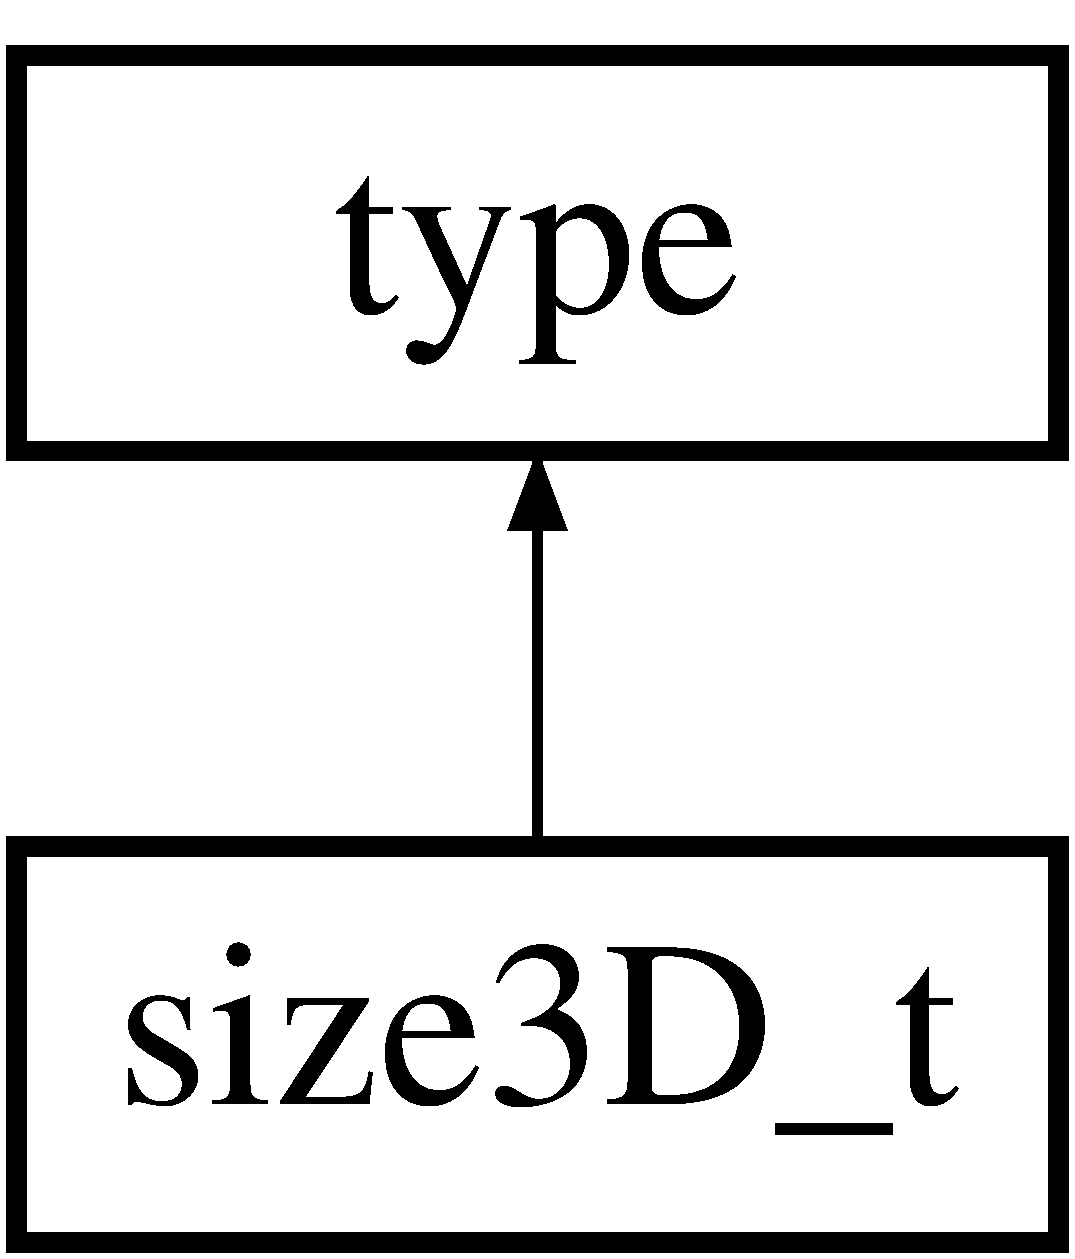
\includegraphics[height=2.000000cm]{classsize3D__t}
\end{center}
\end{figure}
\subsection*{Public Types}
\begin{DoxyCompactItemize}
\item 
typedef \-::\hyperlink{namespacexml__schema_acfa24ac68e1a188e7f44c36f7a158bf4}{xml\-\_\-schema\-::int\-\_\-} \hyperlink{classsize3D__t_a7d35a723ccd7d990ae9b91f8d8856a69}{width\-\_\-type}
\item 
typedef \\*
\-::xsd\-::cxx\-::tree\-::traits\\*
$<$ \hyperlink{classsize3D__t_a7d35a723ccd7d990ae9b91f8d8856a69}{width\-\_\-type}, char $>$ \hyperlink{classsize3D__t_a98b58b7e1830b6e07c64d7a6dd10aae5}{width\-\_\-traits}
\item 
typedef \-::\hyperlink{namespacexml__schema_acfa24ac68e1a188e7f44c36f7a158bf4}{xml\-\_\-schema\-::int\-\_\-} \hyperlink{classsize3D__t_adc8341bc222084318ef434ea22833f69}{height\-\_\-type}
\item 
typedef \\*
\-::xsd\-::cxx\-::tree\-::traits\\*
$<$ \hyperlink{classsize3D__t_adc8341bc222084318ef434ea22833f69}{height\-\_\-type}, char $>$ \hyperlink{classsize3D__t_a915f1e11ad383a66bf5263c0f71c1b45}{height\-\_\-traits}
\item 
typedef \-::\hyperlink{namespacexml__schema_acfa24ac68e1a188e7f44c36f7a158bf4}{xml\-\_\-schema\-::int\-\_\-} \hyperlink{classsize3D__t_acc72088c95989e8ecee3fef8118cb91e}{depth\-\_\-type}
\item 
typedef \\*
\-::xsd\-::cxx\-::tree\-::traits\\*
$<$ \hyperlink{classsize3D__t_acc72088c95989e8ecee3fef8118cb91e}{depth\-\_\-type}, char $>$ \hyperlink{classsize3D__t_a0d246a6f5c4afb7d912244a5226f01a0}{depth\-\_\-traits}
\end{DoxyCompactItemize}
\subsection*{Public Member Functions}
\begin{DoxyCompactItemize}
\item 
const \hyperlink{classsize3D__t_a7d35a723ccd7d990ae9b91f8d8856a69}{width\-\_\-type} \& \hyperlink{classsize3D__t_a6e1d6d6dd0e972c464485d79ac561a25}{width} () const 
\item 
\hyperlink{classsize3D__t_a7d35a723ccd7d990ae9b91f8d8856a69}{width\-\_\-type} \& \hyperlink{classsize3D__t_a858b060e5e4a413554a275ba99ed5721}{width} ()
\item 
void \hyperlink{classsize3D__t_a5af433452dea754f77aa6198cc341d1f}{width} (const \hyperlink{classsize3D__t_a7d35a723ccd7d990ae9b91f8d8856a69}{width\-\_\-type} \&x)
\item 
const \hyperlink{classsize3D__t_adc8341bc222084318ef434ea22833f69}{height\-\_\-type} \& \hyperlink{classsize3D__t_a1c8f9f2245b9aa0398a98c01b7ad4ae3}{height} () const 
\item 
\hyperlink{classsize3D__t_adc8341bc222084318ef434ea22833f69}{height\-\_\-type} \& \hyperlink{classsize3D__t_a78accf4a2dc58f58d7302596b7536857}{height} ()
\item 
void \hyperlink{classsize3D__t_ab324cb8b665c55f78c34f071df3a652c}{height} (const \hyperlink{classsize3D__t_adc8341bc222084318ef434ea22833f69}{height\-\_\-type} \&x)
\item 
const \hyperlink{classsize3D__t_acc72088c95989e8ecee3fef8118cb91e}{depth\-\_\-type} \& \hyperlink{classsize3D__t_a4c20956b2af7b52a01eb34e0c5e6d5ea}{depth} () const 
\item 
\hyperlink{classsize3D__t_acc72088c95989e8ecee3fef8118cb91e}{depth\-\_\-type} \& \hyperlink{classsize3D__t_a32b25671a5c39e9c56a2451063f00b38}{depth} ()
\item 
void \hyperlink{classsize3D__t_afe67f4b26f8c7240b6f0829ad1c90bea}{depth} (const \hyperlink{classsize3D__t_acc72088c95989e8ecee3fef8118cb91e}{depth\-\_\-type} \&x)
\item 
\hyperlink{classsize3D__t_a534bb01312bde80cc754c21b89dcba13}{size3\-D\-\_\-t} (const \hyperlink{classsize3D__t_a7d35a723ccd7d990ae9b91f8d8856a69}{width\-\_\-type} \&, const \hyperlink{classsize3D__t_adc8341bc222084318ef434ea22833f69}{height\-\_\-type} \&, const \hyperlink{classsize3D__t_acc72088c95989e8ecee3fef8118cb91e}{depth\-\_\-type} \&)
\item 
\hyperlink{classsize3D__t_a364f8c8f2f0521af3a5667e65932930d}{size3\-D\-\_\-t} (const \-::xercesc\-::\-D\-O\-M\-Element \&e,\-::\hyperlink{namespacexml__schema_a0612287d030cb2732d31a45b258fdc87}{xml\-\_\-schema\-::flags} f=0,\-::\hyperlink{namespacexml__schema_ada9aa30dc722e93ee2ed7243085402a5}{xml\-\_\-schema\-::container} $\ast$c=0)
\item 
\hyperlink{classsize3D__t_ac5393adac4c8816714a4fbbad067911d}{size3\-D\-\_\-t} (const \hyperlink{classsize3D__t}{size3\-D\-\_\-t} \&x,\-::\hyperlink{namespacexml__schema_a0612287d030cb2732d31a45b258fdc87}{xml\-\_\-schema\-::flags} f=0,\-::\hyperlink{namespacexml__schema_ada9aa30dc722e93ee2ed7243085402a5}{xml\-\_\-schema\-::container} $\ast$c=0)
\item 
virtual \hyperlink{classsize3D__t}{size3\-D\-\_\-t} $\ast$ \hyperlink{classsize3D__t_ada4e1ce7aa535c80b1325f4588ec1844}{\-\_\-clone} (\-::\hyperlink{namespacexml__schema_a0612287d030cb2732d31a45b258fdc87}{xml\-\_\-schema\-::flags} f=0,\-::\hyperlink{namespacexml__schema_ada9aa30dc722e93ee2ed7243085402a5}{xml\-\_\-schema\-::container} $\ast$c=0) const 
\item 
virtual \hyperlink{classsize3D__t_a781511a30f4c1bcd521faab5f8c14c89}{$\sim$size3\-D\-\_\-t} ()
\end{DoxyCompactItemize}
\subsection*{Protected Member Functions}
\begin{DoxyCompactItemize}
\item 
void \hyperlink{classsize3D__t_a61c9c894585f98a117ae18dec35120c7}{parse} (\-::xsd\-::cxx\-::xml\-::dom\-::parser$<$ char $>$ \&,\-::\hyperlink{namespacexml__schema_a0612287d030cb2732d31a45b258fdc87}{xml\-\_\-schema\-::flags})
\end{DoxyCompactItemize}
\subsection*{Protected Attributes}
\begin{DoxyCompactItemize}
\item 
\-::xsd\-::cxx\-::tree\-::one$<$ \hyperlink{classsize3D__t_a7d35a723ccd7d990ae9b91f8d8856a69}{width\-\_\-type} $>$ \hyperlink{classsize3D__t_ac3db384370c18bf31eb74d143c3d8c59}{width\-\_\-}
\item 
\-::xsd\-::cxx\-::tree\-::one\\*
$<$ \hyperlink{classsize3D__t_adc8341bc222084318ef434ea22833f69}{height\-\_\-type} $>$ \hyperlink{classsize3D__t_a33bd3281b2d8ba279f33620da5c43bb3}{height\-\_\-}
\item 
\-::xsd\-::cxx\-::tree\-::one$<$ \hyperlink{classsize3D__t_acc72088c95989e8ecee3fef8118cb91e}{depth\-\_\-type} $>$ \hyperlink{classsize3D__t_a5179c68787cc1fd3f001a602c1d7ea7d}{depth\-\_\-}
\end{DoxyCompactItemize}


\subsection{Member Typedef Documentation}
\hypertarget{classsize3D__t_a0d246a6f5c4afb7d912244a5226f01a0}{\index{size3\-D\-\_\-t@{size3\-D\-\_\-t}!depth\-\_\-traits@{depth\-\_\-traits}}
\index{depth\-\_\-traits@{depth\-\_\-traits}!size3D_t@{size3\-D\-\_\-t}}
\subsubsection[{depth\-\_\-traits}]{\setlength{\rightskip}{0pt plus 5cm}typedef \-::xsd\-::cxx\-::tree\-::traits$<$ {\bf depth\-\_\-type}, char $>$ {\bf size3\-D\-\_\-t\-::depth\-\_\-traits}}}\label{classsize3D__t_a0d246a6f5c4afb7d912244a5226f01a0}
\hypertarget{classsize3D__t_acc72088c95989e8ecee3fef8118cb91e}{\index{size3\-D\-\_\-t@{size3\-D\-\_\-t}!depth\-\_\-type@{depth\-\_\-type}}
\index{depth\-\_\-type@{depth\-\_\-type}!size3D_t@{size3\-D\-\_\-t}}
\subsubsection[{depth\-\_\-type}]{\setlength{\rightskip}{0pt plus 5cm}typedef \-::{\bf xml\-\_\-schema\-::int\-\_\-} {\bf size3\-D\-\_\-t\-::depth\-\_\-type}}}\label{classsize3D__t_acc72088c95989e8ecee3fef8118cb91e}
\hypertarget{classsize3D__t_a915f1e11ad383a66bf5263c0f71c1b45}{\index{size3\-D\-\_\-t@{size3\-D\-\_\-t}!height\-\_\-traits@{height\-\_\-traits}}
\index{height\-\_\-traits@{height\-\_\-traits}!size3D_t@{size3\-D\-\_\-t}}
\subsubsection[{height\-\_\-traits}]{\setlength{\rightskip}{0pt plus 5cm}typedef \-::xsd\-::cxx\-::tree\-::traits$<$ {\bf height\-\_\-type}, char $>$ {\bf size3\-D\-\_\-t\-::height\-\_\-traits}}}\label{classsize3D__t_a915f1e11ad383a66bf5263c0f71c1b45}
\hypertarget{classsize3D__t_adc8341bc222084318ef434ea22833f69}{\index{size3\-D\-\_\-t@{size3\-D\-\_\-t}!height\-\_\-type@{height\-\_\-type}}
\index{height\-\_\-type@{height\-\_\-type}!size3D_t@{size3\-D\-\_\-t}}
\subsubsection[{height\-\_\-type}]{\setlength{\rightskip}{0pt plus 5cm}typedef \-::{\bf xml\-\_\-schema\-::int\-\_\-} {\bf size3\-D\-\_\-t\-::height\-\_\-type}}}\label{classsize3D__t_adc8341bc222084318ef434ea22833f69}
\hypertarget{classsize3D__t_a98b58b7e1830b6e07c64d7a6dd10aae5}{\index{size3\-D\-\_\-t@{size3\-D\-\_\-t}!width\-\_\-traits@{width\-\_\-traits}}
\index{width\-\_\-traits@{width\-\_\-traits}!size3D_t@{size3\-D\-\_\-t}}
\subsubsection[{width\-\_\-traits}]{\setlength{\rightskip}{0pt plus 5cm}typedef \-::xsd\-::cxx\-::tree\-::traits$<$ {\bf width\-\_\-type}, char $>$ {\bf size3\-D\-\_\-t\-::width\-\_\-traits}}}\label{classsize3D__t_a98b58b7e1830b6e07c64d7a6dd10aae5}
\hypertarget{classsize3D__t_a7d35a723ccd7d990ae9b91f8d8856a69}{\index{size3\-D\-\_\-t@{size3\-D\-\_\-t}!width\-\_\-type@{width\-\_\-type}}
\index{width\-\_\-type@{width\-\_\-type}!size3D_t@{size3\-D\-\_\-t}}
\subsubsection[{width\-\_\-type}]{\setlength{\rightskip}{0pt plus 5cm}typedef \-::{\bf xml\-\_\-schema\-::int\-\_\-} {\bf size3\-D\-\_\-t\-::width\-\_\-type}}}\label{classsize3D__t_a7d35a723ccd7d990ae9b91f8d8856a69}


\subsection{Constructor \& Destructor Documentation}
\hypertarget{classsize3D__t_a534bb01312bde80cc754c21b89dcba13}{\index{size3\-D\-\_\-t@{size3\-D\-\_\-t}!size3\-D\-\_\-t@{size3\-D\-\_\-t}}
\index{size3\-D\-\_\-t@{size3\-D\-\_\-t}!size3D_t@{size3\-D\-\_\-t}}
\subsubsection[{size3\-D\-\_\-t}]{\setlength{\rightskip}{0pt plus 5cm}size3\-D\-\_\-t\-::size3\-D\-\_\-t (
\begin{DoxyParamCaption}
\item[{const {\bf width\-\_\-type} \&}]{width, }
\item[{const {\bf height\-\_\-type} \&}]{height, }
\item[{const {\bf depth\-\_\-type} \&}]{depth}
\end{DoxyParamCaption}
)}}\label{classsize3D__t_a534bb01312bde80cc754c21b89dcba13}
\hypertarget{classsize3D__t_a364f8c8f2f0521af3a5667e65932930d}{\index{size3\-D\-\_\-t@{size3\-D\-\_\-t}!size3\-D\-\_\-t@{size3\-D\-\_\-t}}
\index{size3\-D\-\_\-t@{size3\-D\-\_\-t}!size3D_t@{size3\-D\-\_\-t}}
\subsubsection[{size3\-D\-\_\-t}]{\setlength{\rightskip}{0pt plus 5cm}size3\-D\-\_\-t\-::size3\-D\-\_\-t (
\begin{DoxyParamCaption}
\item[{const \-::xercesc\-::\-D\-O\-M\-Element \&}]{e, }
\item[{\-::{\bf xml\-\_\-schema\-::flags}}]{f = {\ttfamily 0}, }
\item[{\-::{\bf xml\-\_\-schema\-::container} $\ast$}]{c = {\ttfamily 0}}
\end{DoxyParamCaption}
)}}\label{classsize3D__t_a364f8c8f2f0521af3a5667e65932930d}
\hypertarget{classsize3D__t_ac5393adac4c8816714a4fbbad067911d}{\index{size3\-D\-\_\-t@{size3\-D\-\_\-t}!size3\-D\-\_\-t@{size3\-D\-\_\-t}}
\index{size3\-D\-\_\-t@{size3\-D\-\_\-t}!size3D_t@{size3\-D\-\_\-t}}
\subsubsection[{size3\-D\-\_\-t}]{\setlength{\rightskip}{0pt plus 5cm}size3\-D\-\_\-t\-::size3\-D\-\_\-t (
\begin{DoxyParamCaption}
\item[{const {\bf size3\-D\-\_\-t} \&}]{x, }
\item[{\-::{\bf xml\-\_\-schema\-::flags}}]{f = {\ttfamily 0}, }
\item[{\-::{\bf xml\-\_\-schema\-::container} $\ast$}]{c = {\ttfamily 0}}
\end{DoxyParamCaption}
)}}\label{classsize3D__t_ac5393adac4c8816714a4fbbad067911d}
\hypertarget{classsize3D__t_a781511a30f4c1bcd521faab5f8c14c89}{\index{size3\-D\-\_\-t@{size3\-D\-\_\-t}!$\sim$size3\-D\-\_\-t@{$\sim$size3\-D\-\_\-t}}
\index{$\sim$size3\-D\-\_\-t@{$\sim$size3\-D\-\_\-t}!size3D_t@{size3\-D\-\_\-t}}
\subsubsection[{$\sim$size3\-D\-\_\-t}]{\setlength{\rightskip}{0pt plus 5cm}size3\-D\-\_\-t\-::$\sim$size3\-D\-\_\-t (
\begin{DoxyParamCaption}
{}
\end{DoxyParamCaption}
)\hspace{0.3cm}{\ttfamily [virtual]}}}\label{classsize3D__t_a781511a30f4c1bcd521faab5f8c14c89}


\subsection{Member Function Documentation}
\hypertarget{classsize3D__t_ada4e1ce7aa535c80b1325f4588ec1844}{\index{size3\-D\-\_\-t@{size3\-D\-\_\-t}!\-\_\-clone@{\-\_\-clone}}
\index{\-\_\-clone@{\-\_\-clone}!size3D_t@{size3\-D\-\_\-t}}
\subsubsection[{\-\_\-clone}]{\setlength{\rightskip}{0pt plus 5cm}{\bf size3\-D\-\_\-t} $\ast$ size3\-D\-\_\-t\-::\-\_\-clone (
\begin{DoxyParamCaption}
\item[{\-::{\bf xml\-\_\-schema\-::flags}}]{f = {\ttfamily 0}, }
\item[{\-::{\bf xml\-\_\-schema\-::container} $\ast$}]{c = {\ttfamily 0}}
\end{DoxyParamCaption}
) const\hspace{0.3cm}{\ttfamily [virtual]}}}\label{classsize3D__t_ada4e1ce7aa535c80b1325f4588ec1844}
\hypertarget{classsize3D__t_a4c20956b2af7b52a01eb34e0c5e6d5ea}{\index{size3\-D\-\_\-t@{size3\-D\-\_\-t}!depth@{depth}}
\index{depth@{depth}!size3D_t@{size3\-D\-\_\-t}}
\subsubsection[{depth}]{\setlength{\rightskip}{0pt plus 5cm}const {\bf size3\-D\-\_\-t\-::depth\-\_\-type} \& size3\-D\-\_\-t\-::depth (
\begin{DoxyParamCaption}
{}
\end{DoxyParamCaption}
) const}}\label{classsize3D__t_a4c20956b2af7b52a01eb34e0c5e6d5ea}
\hypertarget{classsize3D__t_a32b25671a5c39e9c56a2451063f00b38}{\index{size3\-D\-\_\-t@{size3\-D\-\_\-t}!depth@{depth}}
\index{depth@{depth}!size3D_t@{size3\-D\-\_\-t}}
\subsubsection[{depth}]{\setlength{\rightskip}{0pt plus 5cm}{\bf size3\-D\-\_\-t\-::depth\-\_\-type} \& size3\-D\-\_\-t\-::depth (
\begin{DoxyParamCaption}
{}
\end{DoxyParamCaption}
)}}\label{classsize3D__t_a32b25671a5c39e9c56a2451063f00b38}
\hypertarget{classsize3D__t_afe67f4b26f8c7240b6f0829ad1c90bea}{\index{size3\-D\-\_\-t@{size3\-D\-\_\-t}!depth@{depth}}
\index{depth@{depth}!size3D_t@{size3\-D\-\_\-t}}
\subsubsection[{depth}]{\setlength{\rightskip}{0pt plus 5cm}void size3\-D\-\_\-t\-::depth (
\begin{DoxyParamCaption}
\item[{const {\bf depth\-\_\-type} \&}]{x}
\end{DoxyParamCaption}
)}}\label{classsize3D__t_afe67f4b26f8c7240b6f0829ad1c90bea}
\hypertarget{classsize3D__t_a1c8f9f2245b9aa0398a98c01b7ad4ae3}{\index{size3\-D\-\_\-t@{size3\-D\-\_\-t}!height@{height}}
\index{height@{height}!size3D_t@{size3\-D\-\_\-t}}
\subsubsection[{height}]{\setlength{\rightskip}{0pt plus 5cm}const {\bf size3\-D\-\_\-t\-::height\-\_\-type} \& size3\-D\-\_\-t\-::height (
\begin{DoxyParamCaption}
{}
\end{DoxyParamCaption}
) const}}\label{classsize3D__t_a1c8f9f2245b9aa0398a98c01b7ad4ae3}
\hypertarget{classsize3D__t_a78accf4a2dc58f58d7302596b7536857}{\index{size3\-D\-\_\-t@{size3\-D\-\_\-t}!height@{height}}
\index{height@{height}!size3D_t@{size3\-D\-\_\-t}}
\subsubsection[{height}]{\setlength{\rightskip}{0pt plus 5cm}{\bf size3\-D\-\_\-t\-::height\-\_\-type} \& size3\-D\-\_\-t\-::height (
\begin{DoxyParamCaption}
{}
\end{DoxyParamCaption}
)}}\label{classsize3D__t_a78accf4a2dc58f58d7302596b7536857}
\hypertarget{classsize3D__t_ab324cb8b665c55f78c34f071df3a652c}{\index{size3\-D\-\_\-t@{size3\-D\-\_\-t}!height@{height}}
\index{height@{height}!size3D_t@{size3\-D\-\_\-t}}
\subsubsection[{height}]{\setlength{\rightskip}{0pt plus 5cm}void size3\-D\-\_\-t\-::height (
\begin{DoxyParamCaption}
\item[{const {\bf height\-\_\-type} \&}]{x}
\end{DoxyParamCaption}
)}}\label{classsize3D__t_ab324cb8b665c55f78c34f071df3a652c}
\hypertarget{classsize3D__t_a61c9c894585f98a117ae18dec35120c7}{\index{size3\-D\-\_\-t@{size3\-D\-\_\-t}!parse@{parse}}
\index{parse@{parse}!size3D_t@{size3\-D\-\_\-t}}
\subsubsection[{parse}]{\setlength{\rightskip}{0pt plus 5cm}void size3\-D\-\_\-t\-::parse (
\begin{DoxyParamCaption}
\item[{\-::xsd\-::cxx\-::xml\-::dom\-::parser$<$ char $>$ \&}]{p, }
\item[{\-::{\bf xml\-\_\-schema\-::flags}}]{f}
\end{DoxyParamCaption}
)\hspace{0.3cm}{\ttfamily [protected]}}}\label{classsize3D__t_a61c9c894585f98a117ae18dec35120c7}
\hypertarget{classsize3D__t_a6e1d6d6dd0e972c464485d79ac561a25}{\index{size3\-D\-\_\-t@{size3\-D\-\_\-t}!width@{width}}
\index{width@{width}!size3D_t@{size3\-D\-\_\-t}}
\subsubsection[{width}]{\setlength{\rightskip}{0pt plus 5cm}const {\bf size3\-D\-\_\-t\-::width\-\_\-type} \& size3\-D\-\_\-t\-::width (
\begin{DoxyParamCaption}
{}
\end{DoxyParamCaption}
) const}}\label{classsize3D__t_a6e1d6d6dd0e972c464485d79ac561a25}
\hypertarget{classsize3D__t_a858b060e5e4a413554a275ba99ed5721}{\index{size3\-D\-\_\-t@{size3\-D\-\_\-t}!width@{width}}
\index{width@{width}!size3D_t@{size3\-D\-\_\-t}}
\subsubsection[{width}]{\setlength{\rightskip}{0pt plus 5cm}{\bf size3\-D\-\_\-t\-::width\-\_\-type} \& size3\-D\-\_\-t\-::width (
\begin{DoxyParamCaption}
{}
\end{DoxyParamCaption}
)}}\label{classsize3D__t_a858b060e5e4a413554a275ba99ed5721}
\hypertarget{classsize3D__t_a5af433452dea754f77aa6198cc341d1f}{\index{size3\-D\-\_\-t@{size3\-D\-\_\-t}!width@{width}}
\index{width@{width}!size3D_t@{size3\-D\-\_\-t}}
\subsubsection[{width}]{\setlength{\rightskip}{0pt plus 5cm}void size3\-D\-\_\-t\-::width (
\begin{DoxyParamCaption}
\item[{const {\bf width\-\_\-type} \&}]{x}
\end{DoxyParamCaption}
)}}\label{classsize3D__t_a5af433452dea754f77aa6198cc341d1f}


\subsection{Member Data Documentation}
\hypertarget{classsize3D__t_a5179c68787cc1fd3f001a602c1d7ea7d}{\index{size3\-D\-\_\-t@{size3\-D\-\_\-t}!depth\-\_\-@{depth\-\_\-}}
\index{depth\-\_\-@{depth\-\_\-}!size3D_t@{size3\-D\-\_\-t}}
\subsubsection[{depth\-\_\-}]{\setlength{\rightskip}{0pt plus 5cm}\-::xsd\-::cxx\-::tree\-::one$<$ {\bf depth\-\_\-type} $>$ size3\-D\-\_\-t\-::depth\-\_\-\hspace{0.3cm}{\ttfamily [protected]}}}\label{classsize3D__t_a5179c68787cc1fd3f001a602c1d7ea7d}
\hypertarget{classsize3D__t_a33bd3281b2d8ba279f33620da5c43bb3}{\index{size3\-D\-\_\-t@{size3\-D\-\_\-t}!height\-\_\-@{height\-\_\-}}
\index{height\-\_\-@{height\-\_\-}!size3D_t@{size3\-D\-\_\-t}}
\subsubsection[{height\-\_\-}]{\setlength{\rightskip}{0pt plus 5cm}\-::xsd\-::cxx\-::tree\-::one$<$ {\bf height\-\_\-type} $>$ size3\-D\-\_\-t\-::height\-\_\-\hspace{0.3cm}{\ttfamily [protected]}}}\label{classsize3D__t_a33bd3281b2d8ba279f33620da5c43bb3}
\hypertarget{classsize3D__t_ac3db384370c18bf31eb74d143c3d8c59}{\index{size3\-D\-\_\-t@{size3\-D\-\_\-t}!width\-\_\-@{width\-\_\-}}
\index{width\-\_\-@{width\-\_\-}!size3D_t@{size3\-D\-\_\-t}}
\subsubsection[{width\-\_\-}]{\setlength{\rightskip}{0pt plus 5cm}\-::xsd\-::cxx\-::tree\-::one$<$ {\bf width\-\_\-type} $>$ size3\-D\-\_\-t\-::width\-\_\-\hspace{0.3cm}{\ttfamily [protected]}}}\label{classsize3D__t_ac3db384370c18bf31eb74d143c3d8c59}


The documentation for this class was generated from the following files\-:\begin{DoxyCompactItemize}
\item 
src/utils/\hyperlink{InputCuboids_8h}{Input\-Cuboids.\-h}\item 
src/utils/\hyperlink{InputCuboids_8cpp}{Input\-Cuboids.\-cpp}\end{DoxyCompactItemize}

\hypertarget{classSphere}{\section{Sphere Class Reference}
\label{classSphere}\index{Sphere@{Sphere}}
}


This is a class representing a 3\-D sphere of particles.  




{\ttfamily \#include $<$Sphere.\-h$>$}

\subsection*{Public Member Functions}
\begin{DoxyCompactItemize}
\item 
\hyperlink{classSphere_a890a63ff583cb88e7ec4e840b4ef5eb9}{Sphere} ()
\item 
\hyperlink{classSphere_a9644e05e957d1e94c6b49c791ced6af5}{Sphere} (\hyperlink{classutils_1_1Vector}{utils\-::\-Vector}$<$ double, 3 $>$ \hyperlink{classSphere_a23d3e7709e2cabae2608d470a1edcece}{center}, \hyperlink{classutils_1_1Vector}{utils\-::\-Vector}$<$ double, 3 $>$ \hyperlink{classSphere_a93f232ff2747403c36fbe0513155da89}{start\-V}, double \hyperlink{classSphere_a2cd2b54a44a8c48132a37bc99e9540a3}{mean\-V}, double \hyperlink{classSphere_aa98b073187155748b82f6675aa65a2d3}{m}, int \hyperlink{classSphere_ab4adc2969e56bb99f4a88fac7a390313}{radius}, double \hyperlink{classSphere_a0e2523061bbf7ebef88534efeefe91f9}{mesh\-Width}, int \hyperlink{classSphere_ae52652f5262aa5268f2442a0c598917e}{par\-Type}, double \hyperlink{classSphere_ada633ebd567ecc2c88b9e31d7de8fc31}{E\-P\-S\-I\-L\-O\-N}, double \hyperlink{classSphere_a1515a874e99244d9c4bc2bd782a4eb7f}{S\-I\-G\-M\-A})
\item 
\hyperlink{classutils_1_1Vector}{utils\-::\-Vector}$<$ double, 3 $>$ \& \hyperlink{classSphere_ae6672bb1f28f220707e0733fcd861683}{get\-Center} ()
\item 
\hyperlink{classutils_1_1Vector}{utils\-::\-Vector}$<$ double, 3 $>$ \& \hyperlink{classSphere_aff78cca177f74fb8f2d8bff01ae29ca8}{get\-Start\-V} ()
\item 
double \& \hyperlink{classSphere_ae491e83c8253a9ef35f2be41be191757}{get\-Mean\-V} ()
\item 
double \& \hyperlink{classSphere_a7364ad539afc14bea43529e6cbb5ea45}{get\-M} ()
\item 
int \& \hyperlink{classSphere_a8a7b55dc6859aeb70405176ad2669ee8}{get\-Radius} ()
\item 
double \& \hyperlink{classSphere_a8796dba65ece80813b560fefdebf3ed0}{get\-Mesh\-Width} ()
\item 
std\-::list$<$ \hyperlink{classParticle}{Particle} $>$ \& \hyperlink{classSphere_a8d8082fba50dadba0afc58877d126603}{get\-Sphere} ()
\item 
int \& \hyperlink{classSphere_a5023edd8787a02cb96bfc4ce9d6f3335}{get\-Type} ()
\item 
double \hyperlink{classSphere_a647815fa5959a710a15b3b58b1748326}{get\-Epsilon} ()
\item 
double \hyperlink{classSphere_ade101a82ae3fa2c93969f0316dc8ec9c}{get\-Sigma} ()
\item 
virtual \hyperlink{classSphere_a569c071e50a3e11f678630ee1a17737e}{$\sim$\-Sphere} ()
\end{DoxyCompactItemize}
\subsection*{Private Member Functions}
\begin{DoxyCompactItemize}
\item 
void \hyperlink{classSphere_a0c92cd51e271f64c97c96fc5f4d775a8}{init\-List\-Of\-Centers} ()
\item 
void \hyperlink{classSphere_acbe46e167b61e7b1d1fb4b80ad45f386}{init\-List\-Of\-Radii} ()
\item 
void \hyperlink{classSphere_add9cb3b5fc594012c8e0f64556db02f9}{plot} (\hyperlink{classutils_1_1Vector}{utils\-::\-Vector}$<$ double, 3 $>$ temp\-Center, int x, int y)
\item 
void \hyperlink{classSphere_a7069d3583fbb47c93d825306df9f2f4c}{draw\-Vertical\-Line} (\hyperlink{classutils_1_1Vector}{utils\-::\-Vector}$<$ double, 3 $>$ temp\-Center, int upper\-Height)
\item 
void \hyperlink{classSphere_ac81f8d066b948468d700047994934eda}{draw\-Circle\-Area} (\hyperlink{classutils_1_1Vector}{utils\-::\-Vector}$<$ double, 3 $>$ temp\-Center, int rad)
\item 
void \hyperlink{classSphere_a208034eeb2308ab02ca8ea36d23f45af}{draw\-Biggest\-Circle\-Area} ()
\end{DoxyCompactItemize}
\subsection*{Private Attributes}
\begin{DoxyCompactItemize}
\item 
\hyperlink{classutils_1_1Vector}{utils\-::\-Vector}$<$ double, 3 $>$ \hyperlink{classSphere_a23d3e7709e2cabae2608d470a1edcece}{center}
\item 
\hyperlink{classutils_1_1Vector}{utils\-::\-Vector}$<$ double, 3 $>$ \hyperlink{classSphere_a93f232ff2747403c36fbe0513155da89}{start\-V}
\item 
double \hyperlink{classSphere_a2cd2b54a44a8c48132a37bc99e9540a3}{mean\-V}
\item 
double \hyperlink{classSphere_aa98b073187155748b82f6675aa65a2d3}{m}
\item 
int \hyperlink{classSphere_ab4adc2969e56bb99f4a88fac7a390313}{radius}
\item 
double \hyperlink{classSphere_a0e2523061bbf7ebef88534efeefe91f9}{mesh\-Width}
\item 
int \hyperlink{classSphere_ae52652f5262aa5268f2442a0c598917e}{par\-Type}
\item 
double \hyperlink{classSphere_ada633ebd567ecc2c88b9e31d7de8fc31}{E\-P\-S\-I\-L\-O\-N}
\item 
double \hyperlink{classSphere_a1515a874e99244d9c4bc2bd782a4eb7f}{S\-I\-G\-M\-A}
\item 
std\-::list$<$ \hyperlink{classParticle}{Particle} $>$ \hyperlink{classSphere_a0f3aa4c3e86814bb8f7061dc83fc992c}{sph}
\item 
std\-::vector$<$ \hyperlink{classutils_1_1Vector}{utils\-::\-Vector}\\*
$<$ double, 3 $>$ $>$ \hyperlink{classSphere_a9c74234600792e31954bcbf58e692b95}{list\-Of\-Centers}
\item 
std\-::vector$<$ int $>$ \hyperlink{classSphere_a97986825b799049cdc4ffbe535e23200}{list\-Of\-Radii}
\end{DoxyCompactItemize}


\subsection{Detailed Description}
This is a class representing a 3\-D sphere of particles. 

One sphere can save a 3\-D set of particles, which are located next to each other. There is no isolated particle in one sphere. 

\subsection{Constructor \& Destructor Documentation}
\hypertarget{classSphere_a890a63ff583cb88e7ec4e840b4ef5eb9}{\index{Sphere@{Sphere}!Sphere@{Sphere}}
\index{Sphere@{Sphere}!Sphere@{Sphere}}
\subsubsection[{Sphere}]{\setlength{\rightskip}{0pt plus 5cm}Sphere\-::\-Sphere (
\begin{DoxyParamCaption}
{}
\end{DoxyParamCaption}
)}}\label{classSphere_a890a63ff583cb88e7ec4e840b4ef5eb9}
Default constructor. \hypertarget{classSphere_a9644e05e957d1e94c6b49c791ced6af5}{\index{Sphere@{Sphere}!Sphere@{Sphere}}
\index{Sphere@{Sphere}!Sphere@{Sphere}}
\subsubsection[{Sphere}]{\setlength{\rightskip}{0pt plus 5cm}Sphere\-::\-Sphere (
\begin{DoxyParamCaption}
\item[{{\bf utils\-::\-Vector}$<$ double, 3 $>$}]{center, }
\item[{{\bf utils\-::\-Vector}$<$ double, 3 $>$}]{start\-V, }
\item[{double}]{mean\-V, }
\item[{double}]{m, }
\item[{int}]{radius, }
\item[{double}]{mesh\-Width, }
\item[{int}]{par\-Type, }
\item[{double}]{E\-P\-S\-I\-L\-O\-N, }
\item[{double}]{S\-I\-G\-M\-A}
\end{DoxyParamCaption}
)}}\label{classSphere_a9644e05e957d1e94c6b49c791ced6af5}
The main constructor.

Constructs a new sphere with all information needed. 
\begin{DoxyParams}[1]{Parameters}
\mbox{\tt in}  & {\em center} & \hyperlink{classSphere}{Sphere}'s center's location. \\
\hline
\mbox{\tt in}  & {\em start\-V} & Start velocity of all particles in the beginning. \\
\hline
\mbox{\tt in}  & {\em mean\-V} & Mean velocity (aka. brownian factor) of each partcile in sphere. \\
\hline
\mbox{\tt in}  & {\em m} & Mass of each particle in sphere. \\
\hline
\mbox{\tt in}  & {\em radius} & Radius of the sphere in particles (int not double!). \\
\hline
\mbox{\tt in}  & {\em mesh\-Width} & The mesh distance between every 2 nearest particles of sphere. \\
\hline
\mbox{\tt in}  & {\em par\-Type} & \hyperlink{classParticle}{Particle} type of sphere. \\
\hline
\mbox{\tt in}  & {\em E\-P\-S\-I\-L\-O\-N} & For Lennard Jones Force. \\
\hline
\mbox{\tt in}  & {\em S\-I\-G\-M\-A} & For Lennard Jones Force. \\
\hline
\end{DoxyParams}
\hypertarget{classSphere_a569c071e50a3e11f678630ee1a17737e}{\index{Sphere@{Sphere}!$\sim$\-Sphere@{$\sim$\-Sphere}}
\index{$\sim$\-Sphere@{$\sim$\-Sphere}!Sphere@{Sphere}}
\subsubsection[{$\sim$\-Sphere}]{\setlength{\rightskip}{0pt plus 5cm}Sphere\-::$\sim$\-Sphere (
\begin{DoxyParamCaption}
{}
\end{DoxyParamCaption}
)\hspace{0.3cm}{\ttfamily [virtual]}}}\label{classSphere_a569c071e50a3e11f678630ee1a17737e}


\subsection{Member Function Documentation}
\hypertarget{classSphere_a208034eeb2308ab02ca8ea36d23f45af}{\index{Sphere@{Sphere}!draw\-Biggest\-Circle\-Area@{draw\-Biggest\-Circle\-Area}}
\index{draw\-Biggest\-Circle\-Area@{draw\-Biggest\-Circle\-Area}!Sphere@{Sphere}}
\subsubsection[{draw\-Biggest\-Circle\-Area}]{\setlength{\rightskip}{0pt plus 5cm}void Sphere\-::draw\-Biggest\-Circle\-Area (
\begin{DoxyParamCaption}
{}
\end{DoxyParamCaption}
)\hspace{0.3cm}{\ttfamily [private]}}}\label{classSphere_a208034eeb2308ab02ca8ea36d23f45af}
Draw the biggest circle of the sphere. Also fills list\-Of\-Centers and list\-Of\-Radii Is private and needed for building the sphere (Alternative 2\-: Bresenham). \hypertarget{classSphere_ac81f8d066b948468d700047994934eda}{\index{Sphere@{Sphere}!draw\-Circle\-Area@{draw\-Circle\-Area}}
\index{draw\-Circle\-Area@{draw\-Circle\-Area}!Sphere@{Sphere}}
\subsubsection[{draw\-Circle\-Area}]{\setlength{\rightskip}{0pt plus 5cm}void Sphere\-::draw\-Circle\-Area (
\begin{DoxyParamCaption}
\item[{{\bf utils\-::\-Vector}$<$ double, 3 $>$}]{temp\-Center, }
\item[{int}]{rad}
\end{DoxyParamCaption}
)\hspace{0.3cm}{\ttfamily [private]}}}\label{classSphere_ac81f8d066b948468d700047994934eda}
Draw a circle with given radius and center. Is private and needed for building the sphere (Alternative 2\-: Bresenham). To build a sphere we have to make (2$\ast$radius + 1) circles.


\begin{DoxyParams}[1]{Parameters}
\mbox{\tt in}  & {\em temp\-Center,\-:} & the coordinates of the center of the C\-U\-R\-R\-E\-N\-T circle. \\
\hline
\mbox{\tt in}  & {\em rad,\-:} & radius of the current circle. \\
\hline
\end{DoxyParams}
\hypertarget{classSphere_a7069d3583fbb47c93d825306df9f2f4c}{\index{Sphere@{Sphere}!draw\-Vertical\-Line@{draw\-Vertical\-Line}}
\index{draw\-Vertical\-Line@{draw\-Vertical\-Line}!Sphere@{Sphere}}
\subsubsection[{draw\-Vertical\-Line}]{\setlength{\rightskip}{0pt plus 5cm}void Sphere\-::draw\-Vertical\-Line (
\begin{DoxyParamCaption}
\item[{{\bf utils\-::\-Vector}$<$ double, 3 $>$}]{temp\-Center, }
\item[{int}]{upper\-Height}
\end{DoxyParamCaption}
)\hspace{0.3cm}{\ttfamily [private]}}}\label{classSphere_a7069d3583fbb47c93d825306df9f2f4c}
Draw a single vertical line in the current circle. Length = 2$\ast$upper\-Height + 1 Is private and needed for building the sphere (Alternative 2\-: Bresenham).


\begin{DoxyParams}[1]{Parameters}
\mbox{\tt in}  & {\em temp\-Center,\-:} & the coordinates of the center of the C\-U\-R\-R\-E\-N\-T vertical line. \\
\hline
\mbox{\tt in}  & {\em upper\-Height,\-:} & Since every line is symmetric, only the upper length is needed. \\
\hline
\mbox{\tt out}  & {\em sph,\-:} & the new particle will be stored here. \\
\hline
\end{DoxyParams}
\hypertarget{classSphere_ae6672bb1f28f220707e0733fcd861683}{\index{Sphere@{Sphere}!get\-Center@{get\-Center}}
\index{get\-Center@{get\-Center}!Sphere@{Sphere}}
\subsubsection[{get\-Center}]{\setlength{\rightskip}{0pt plus 5cm}{\bf utils\-::\-Vector}$<$ double, 3 $>$ \& Sphere\-::get\-Center (
\begin{DoxyParamCaption}
{}
\end{DoxyParamCaption}
)}}\label{classSphere_ae6672bb1f28f220707e0733fcd861683}
\begin{DoxyReturn}{Returns}
\hyperlink{classSphere}{Sphere}'s center's location. 
\end{DoxyReturn}
\hypertarget{classSphere_a647815fa5959a710a15b3b58b1748326}{\index{Sphere@{Sphere}!get\-Epsilon@{get\-Epsilon}}
\index{get\-Epsilon@{get\-Epsilon}!Sphere@{Sphere}}
\subsubsection[{get\-Epsilon}]{\setlength{\rightskip}{0pt plus 5cm}double Sphere\-::get\-Epsilon (
\begin{DoxyParamCaption}
{}
\end{DoxyParamCaption}
)}}\label{classSphere_a647815fa5959a710a15b3b58b1748326}
\begin{DoxyReturn}{Returns}
\hyperlink{classCuboid}{Cuboid}'s epsilon for Lennard Jones Force. 
\end{DoxyReturn}
\hypertarget{classSphere_a7364ad539afc14bea43529e6cbb5ea45}{\index{Sphere@{Sphere}!get\-M@{get\-M}}
\index{get\-M@{get\-M}!Sphere@{Sphere}}
\subsubsection[{get\-M}]{\setlength{\rightskip}{0pt plus 5cm}double \& Sphere\-::get\-M (
\begin{DoxyParamCaption}
{}
\end{DoxyParamCaption}
)}}\label{classSphere_a7364ad539afc14bea43529e6cbb5ea45}
\begin{DoxyReturn}{Returns}
Mass of each particle. 
\end{DoxyReturn}
\hypertarget{classSphere_ae491e83c8253a9ef35f2be41be191757}{\index{Sphere@{Sphere}!get\-Mean\-V@{get\-Mean\-V}}
\index{get\-Mean\-V@{get\-Mean\-V}!Sphere@{Sphere}}
\subsubsection[{get\-Mean\-V}]{\setlength{\rightskip}{0pt plus 5cm}double \& Sphere\-::get\-Mean\-V (
\begin{DoxyParamCaption}
{}
\end{DoxyParamCaption}
)}}\label{classSphere_ae491e83c8253a9ef35f2be41be191757}
\begin{DoxyReturn}{Returns}
Mean velocity of particles. 
\end{DoxyReturn}
\hypertarget{classSphere_a8796dba65ece80813b560fefdebf3ed0}{\index{Sphere@{Sphere}!get\-Mesh\-Width@{get\-Mesh\-Width}}
\index{get\-Mesh\-Width@{get\-Mesh\-Width}!Sphere@{Sphere}}
\subsubsection[{get\-Mesh\-Width}]{\setlength{\rightskip}{0pt plus 5cm}double \& Sphere\-::get\-Mesh\-Width (
\begin{DoxyParamCaption}
{}
\end{DoxyParamCaption}
)}}\label{classSphere_a8796dba65ece80813b560fefdebf3ed0}
\begin{DoxyReturn}{Returns}
Mesh distance between every 2 nearest particles. 
\end{DoxyReturn}
\hypertarget{classSphere_a8a7b55dc6859aeb70405176ad2669ee8}{\index{Sphere@{Sphere}!get\-Radius@{get\-Radius}}
\index{get\-Radius@{get\-Radius}!Sphere@{Sphere}}
\subsubsection[{get\-Radius}]{\setlength{\rightskip}{0pt plus 5cm}int \& Sphere\-::get\-Radius (
\begin{DoxyParamCaption}
{}
\end{DoxyParamCaption}
)}}\label{classSphere_a8a7b55dc6859aeb70405176ad2669ee8}
\begin{DoxyReturn}{Returns}
Radius of the sphere. 
\end{DoxyReturn}
\hypertarget{classSphere_ade101a82ae3fa2c93969f0316dc8ec9c}{\index{Sphere@{Sphere}!get\-Sigma@{get\-Sigma}}
\index{get\-Sigma@{get\-Sigma}!Sphere@{Sphere}}
\subsubsection[{get\-Sigma}]{\setlength{\rightskip}{0pt plus 5cm}double Sphere\-::get\-Sigma (
\begin{DoxyParamCaption}
{}
\end{DoxyParamCaption}
)}}\label{classSphere_ade101a82ae3fa2c93969f0316dc8ec9c}
\begin{DoxyReturn}{Returns}
\hyperlink{classCuboid}{Cuboid}'s sigma for Lennard Jones Force. 
\end{DoxyReturn}
\hypertarget{classSphere_a8d8082fba50dadba0afc58877d126603}{\index{Sphere@{Sphere}!get\-Sphere@{get\-Sphere}}
\index{get\-Sphere@{get\-Sphere}!Sphere@{Sphere}}
\subsubsection[{get\-Sphere}]{\setlength{\rightskip}{0pt plus 5cm}std\-::list$<$ {\bf Particle} $>$ \& Sphere\-::get\-Sphere (
\begin{DoxyParamCaption}
{}
\end{DoxyParamCaption}
)}}\label{classSphere_a8d8082fba50dadba0afc58877d126603}
\begin{DoxyReturn}{Returns}
List of stored particles in the sphere. 
\end{DoxyReturn}
\hypertarget{classSphere_aff78cca177f74fb8f2d8bff01ae29ca8}{\index{Sphere@{Sphere}!get\-Start\-V@{get\-Start\-V}}
\index{get\-Start\-V@{get\-Start\-V}!Sphere@{Sphere}}
\subsubsection[{get\-Start\-V}]{\setlength{\rightskip}{0pt plus 5cm}{\bf utils\-::\-Vector}$<$ double, 3 $>$ \& Sphere\-::get\-Start\-V (
\begin{DoxyParamCaption}
{}
\end{DoxyParamCaption}
)}}\label{classSphere_aff78cca177f74fb8f2d8bff01ae29ca8}
\begin{DoxyReturn}{Returns}
Velocity at the beginning of each particle in sphere. 
\end{DoxyReturn}
\hypertarget{classSphere_a5023edd8787a02cb96bfc4ce9d6f3335}{\index{Sphere@{Sphere}!get\-Type@{get\-Type}}
\index{get\-Type@{get\-Type}!Sphere@{Sphere}}
\subsubsection[{get\-Type}]{\setlength{\rightskip}{0pt plus 5cm}int \& Sphere\-::get\-Type (
\begin{DoxyParamCaption}
{}
\end{DoxyParamCaption}
)}}\label{classSphere_a5023edd8787a02cb96bfc4ce9d6f3335}
\begin{DoxyReturn}{Returns}
particle type of the sphere. 
\end{DoxyReturn}
\hypertarget{classSphere_a0c92cd51e271f64c97c96fc5f4d775a8}{\index{Sphere@{Sphere}!init\-List\-Of\-Centers@{init\-List\-Of\-Centers}}
\index{init\-List\-Of\-Centers@{init\-List\-Of\-Centers}!Sphere@{Sphere}}
\subsubsection[{init\-List\-Of\-Centers}]{\setlength{\rightskip}{0pt plus 5cm}void Sphere\-::init\-List\-Of\-Centers (
\begin{DoxyParamCaption}
{}
\end{DoxyParamCaption}
)\hspace{0.3cm}{\ttfamily [private]}}}\label{classSphere_a0c92cd51e271f64c97c96fc5f4d775a8}
Initializes list\-Of\-Centers\-: list\-Of\-Centers\mbox{[}radius\mbox{]} = center (the biggest circle) Is private and needed for building the sphere (Alternative 2\-: Bresenham). Must be called before \hyperlink{classSphere_a208034eeb2308ab02ca8ea36d23f45af}{draw\-Biggest\-Circle\-Area()}. \hypertarget{classSphere_acbe46e167b61e7b1d1fb4b80ad45f386}{\index{Sphere@{Sphere}!init\-List\-Of\-Radii@{init\-List\-Of\-Radii}}
\index{init\-List\-Of\-Radii@{init\-List\-Of\-Radii}!Sphere@{Sphere}}
\subsubsection[{init\-List\-Of\-Radii}]{\setlength{\rightskip}{0pt plus 5cm}void Sphere\-::init\-List\-Of\-Radii (
\begin{DoxyParamCaption}
{}
\end{DoxyParamCaption}
)\hspace{0.3cm}{\ttfamily [private]}}}\label{classSphere_acbe46e167b61e7b1d1fb4b80ad45f386}
Initializes list\-Of\-Radii\-: list\-Of\-Radii\mbox{[}radius\mbox{]} = radius (the biggest circle) Is private and needed for building the sphere (Alternative 2\-: Bresenham). Must be called before \hyperlink{classSphere_a208034eeb2308ab02ca8ea36d23f45af}{draw\-Biggest\-Circle\-Area()}. \hypertarget{classSphere_add9cb3b5fc594012c8e0f64556db02f9}{\index{Sphere@{Sphere}!plot@{plot}}
\index{plot@{plot}!Sphere@{Sphere}}
\subsubsection[{plot}]{\setlength{\rightskip}{0pt plus 5cm}void Sphere\-::plot (
\begin{DoxyParamCaption}
\item[{{\bf utils\-::\-Vector}$<$ double, 3 $>$}]{temp\-Center, }
\item[{int}]{x, }
\item[{int}]{y}
\end{DoxyParamCaption}
)\hspace{0.3cm}{\ttfamily [private]}}}\label{classSphere_add9cb3b5fc594012c8e0f64556db02f9}
Push a single particle with the given coordinates into sph\-: Its coordinates are\-: (x$\ast$mesh\-Width, y$\ast$mesh\-Width, temp\-Center\mbox{[}2\mbox{]}) Is private and needed for building the sphere (Alternative 2\-: Bresenham). Is elementary function for building the sphere.


\begin{DoxyParams}{Parameters}
{\em temp\-Center,\-:} & the coordinates of the center of the C\-U\-R\-R\-E\-N\-T circle. \\
\hline
{\em x,\-:} & the horizontal value in the current circle. \\
\hline
{\em y,\-:} & the vertical value in the current circle. \\
\hline
\end{DoxyParams}


\subsection{Member Data Documentation}
\hypertarget{classSphere_a23d3e7709e2cabae2608d470a1edcece}{\index{Sphere@{Sphere}!center@{center}}
\index{center@{center}!Sphere@{Sphere}}
\subsubsection[{center}]{\setlength{\rightskip}{0pt plus 5cm}{\bf utils\-::\-Vector}$<$double, 3$>$ Sphere\-::center\hspace{0.3cm}{\ttfamily [private]}}}\label{classSphere_a23d3e7709e2cabae2608d470a1edcece}
A 3\-D vector indicating the location of the center. \hypertarget{classSphere_ada633ebd567ecc2c88b9e31d7de8fc31}{\index{Sphere@{Sphere}!E\-P\-S\-I\-L\-O\-N@{E\-P\-S\-I\-L\-O\-N}}
\index{E\-P\-S\-I\-L\-O\-N@{E\-P\-S\-I\-L\-O\-N}!Sphere@{Sphere}}
\subsubsection[{E\-P\-S\-I\-L\-O\-N}]{\setlength{\rightskip}{0pt plus 5cm}double Sphere\-::\-E\-P\-S\-I\-L\-O\-N\hspace{0.3cm}{\ttfamily [private]}}}\label{classSphere_ada633ebd567ecc2c88b9e31d7de8fc31}
For Lennard Jones Force. \hypertarget{classSphere_a9c74234600792e31954bcbf58e692b95}{\index{Sphere@{Sphere}!list\-Of\-Centers@{list\-Of\-Centers}}
\index{list\-Of\-Centers@{list\-Of\-Centers}!Sphere@{Sphere}}
\subsubsection[{list\-Of\-Centers}]{\setlength{\rightskip}{0pt plus 5cm}std\-::vector$<${\bf utils\-::\-Vector}$<$double, 3$>$ $>$ Sphere\-::list\-Of\-Centers\hspace{0.3cm}{\ttfamily [private]}}}\label{classSphere_a9c74234600792e31954bcbf58e692b95}
A list of centers of parallel circles along the Oz axis. The distance between 2 nearest circles is mesh\-Width. There are (2$\ast$radius + 1) elements in this list. Is private and needed for building the sphere (Alternative 2\-: Bresenham). \hypertarget{classSphere_a97986825b799049cdc4ffbe535e23200}{\index{Sphere@{Sphere}!list\-Of\-Radii@{list\-Of\-Radii}}
\index{list\-Of\-Radii@{list\-Of\-Radii}!Sphere@{Sphere}}
\subsubsection[{list\-Of\-Radii}]{\setlength{\rightskip}{0pt plus 5cm}std\-::vector$<$int$>$ Sphere\-::list\-Of\-Radii\hspace{0.3cm}{\ttfamily [private]}}}\label{classSphere_a97986825b799049cdc4ffbe535e23200}
A list of radii of parallel circles along the Oz axis, whose centers are stored in list\-Of\-Centers. Both list\-Of\-Centers and list\-Of\-Radii synchronize with eachother. For example\-: The circle with list\-Of\-Centers\mbox{[}i\mbox{]} has radius list\-Of\-Radii\mbox{[}i\mbox{]}. There are (2$\ast$radius + 1) elements in this list. Is private and needed for building the sphere (Alternative 2\-: Bresenham). \hypertarget{classSphere_aa98b073187155748b82f6675aa65a2d3}{\index{Sphere@{Sphere}!m@{m}}
\index{m@{m}!Sphere@{Sphere}}
\subsubsection[{m}]{\setlength{\rightskip}{0pt plus 5cm}double Sphere\-::m\hspace{0.3cm}{\ttfamily [private]}}}\label{classSphere_aa98b073187155748b82f6675aa65a2d3}
Mass of each particle in the sphere. \hypertarget{classSphere_a2cd2b54a44a8c48132a37bc99e9540a3}{\index{Sphere@{Sphere}!mean\-V@{mean\-V}}
\index{mean\-V@{mean\-V}!Sphere@{Sphere}}
\subsubsection[{mean\-V}]{\setlength{\rightskip}{0pt plus 5cm}double Sphere\-::mean\-V\hspace{0.3cm}{\ttfamily [private]}}}\label{classSphere_a2cd2b54a44a8c48132a37bc99e9540a3}
Mean velocity. Used for brownian motion (aka. Brownian Factor). \hypertarget{classSphere_a0e2523061bbf7ebef88534efeefe91f9}{\index{Sphere@{Sphere}!mesh\-Width@{mesh\-Width}}
\index{mesh\-Width@{mesh\-Width}!Sphere@{Sphere}}
\subsubsection[{mesh\-Width}]{\setlength{\rightskip}{0pt plus 5cm}double Sphere\-::mesh\-Width\hspace{0.3cm}{\ttfamily [private]}}}\label{classSphere_a0e2523061bbf7ebef88534efeefe91f9}
The mesh distance between 2 particles. \hypertarget{classSphere_ae52652f5262aa5268f2442a0c598917e}{\index{Sphere@{Sphere}!par\-Type@{par\-Type}}
\index{par\-Type@{par\-Type}!Sphere@{Sphere}}
\subsubsection[{par\-Type}]{\setlength{\rightskip}{0pt plus 5cm}int Sphere\-::par\-Type\hspace{0.3cm}{\ttfamily [private]}}}\label{classSphere_ae52652f5262aa5268f2442a0c598917e}
Type of particles in sphere. \hypertarget{classSphere_ab4adc2969e56bb99f4a88fac7a390313}{\index{Sphere@{Sphere}!radius@{radius}}
\index{radius@{radius}!Sphere@{Sphere}}
\subsubsection[{radius}]{\setlength{\rightskip}{0pt plus 5cm}int Sphere\-::radius\hspace{0.3cm}{\ttfamily [private]}}}\label{classSphere_ab4adc2969e56bb99f4a88fac7a390313}
The sphere's radius in particles (an int number!). The real double radius is radius$\ast$mesh\-Width. \hypertarget{classSphere_a1515a874e99244d9c4bc2bd782a4eb7f}{\index{Sphere@{Sphere}!S\-I\-G\-M\-A@{S\-I\-G\-M\-A}}
\index{S\-I\-G\-M\-A@{S\-I\-G\-M\-A}!Sphere@{Sphere}}
\subsubsection[{S\-I\-G\-M\-A}]{\setlength{\rightskip}{0pt plus 5cm}double Sphere\-::\-S\-I\-G\-M\-A\hspace{0.3cm}{\ttfamily [private]}}}\label{classSphere_a1515a874e99244d9c4bc2bd782a4eb7f}
For Lennard Jones Force. \hypertarget{classSphere_a0f3aa4c3e86814bb8f7061dc83fc992c}{\index{Sphere@{Sphere}!sph@{sph}}
\index{sph@{sph}!Sphere@{Sphere}}
\subsubsection[{sph}]{\setlength{\rightskip}{0pt plus 5cm}std\-::list$<${\bf Particle}$>$ Sphere\-::sph\hspace{0.3cm}{\ttfamily [private]}}}\label{classSphere_a0f3aa4c3e86814bb8f7061dc83fc992c}
The list of particles stored in this sphere. \hypertarget{classSphere_a93f232ff2747403c36fbe0513155da89}{\index{Sphere@{Sphere}!start\-V@{start\-V}}
\index{start\-V@{start\-V}!Sphere@{Sphere}}
\subsubsection[{start\-V}]{\setlength{\rightskip}{0pt plus 5cm}{\bf utils\-::\-Vector}$<$double, 3$>$ Sphere\-::start\-V\hspace{0.3cm}{\ttfamily [private]}}}\label{classSphere_a93f232ff2747403c36fbe0513155da89}
A 3\-D vector indicating the start velocity. 

The documentation for this class was generated from the following files\-:\begin{DoxyCompactItemize}
\item 
src/\hyperlink{Sphere_8h}{Sphere.\-h}\item 
src/\hyperlink{Sphere_8cpp}{Sphere.\-cpp}\end{DoxyCompactItemize}

\hypertarget{classsphere__t}{\section{sphere\-\_\-t Class Reference}
\label{classsphere__t}\index{sphere\-\_\-t@{sphere\-\_\-t}}
}


{\ttfamily \#include $<$Input\-Spheres.\-h$>$}

Inheritance diagram for sphere\-\_\-t\-:\begin{figure}[H]
\begin{center}
\leavevmode
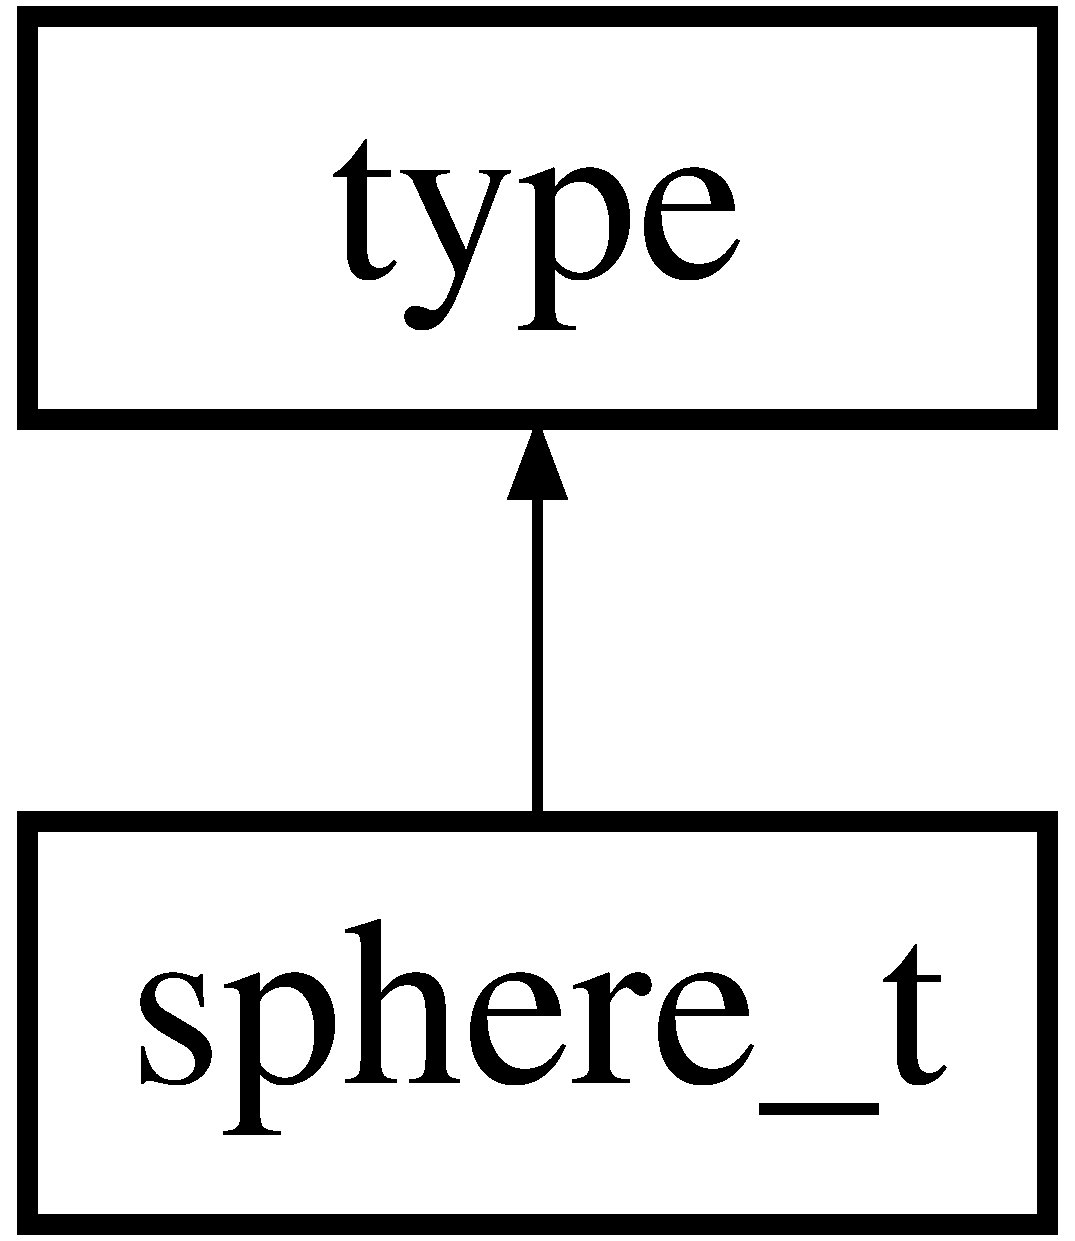
\includegraphics[height=2.000000cm]{classsphere__t}
\end{center}
\end{figure}
\subsection*{Public Types}
\begin{DoxyCompactItemize}
\item 
typedef \-::\hyperlink{namespacexml__schema_a69bfaf24f63a8c18ebd8e21db6b343df}{xml\-\_\-schema\-::decimal} \hyperlink{classsphere__t_a82740a9c5aa0437d973ee3e3caad09ea}{mesh\-Width\-S\-\_\-type}
\item 
typedef \\*
\-::xsd\-::cxx\-::tree\-::traits\\*
$<$ \hyperlink{classsphere__t_a82740a9c5aa0437d973ee3e3caad09ea}{mesh\-Width\-S\-\_\-type}, char,\-::xsd\-::cxx\-::tree\-::schema\-\_\-type\-::decimal $>$ \hyperlink{classsphere__t_a2efcf8f1a1ebfa301c88d3ffa429d1cd}{mesh\-Width\-S\-\_\-traits}
\item 
typedef \-::\hyperlink{namespacexml__schema_a69bfaf24f63a8c18ebd8e21db6b343df}{xml\-\_\-schema\-::decimal} \hyperlink{classsphere__t_a317ddc20b1a4fa225c55721bf12c67b2}{mass\-S\-\_\-type}
\item 
typedef \\*
\-::xsd\-::cxx\-::tree\-::traits\\*
$<$ \hyperlink{classsphere__t_a317ddc20b1a4fa225c55721bf12c67b2}{mass\-S\-\_\-type}, char,\-::xsd\-::cxx\-::tree\-::schema\-\_\-type\-::decimal $>$ \hyperlink{classsphere__t_a7cab3fa5c1e9b5a04581b0262c9f5e5d}{mass\-S\-\_\-traits}
\item 
typedef \-::\hyperlink{namespacexml__schema_a69bfaf24f63a8c18ebd8e21db6b343df}{xml\-\_\-schema\-::decimal} \hyperlink{classsphere__t_a351152e9b83bac409a627037b99a209b}{mean\-V\-S\-\_\-type}
\item 
typedef \\*
\-::xsd\-::cxx\-::tree\-::traits\\*
$<$ \hyperlink{classsphere__t_a351152e9b83bac409a627037b99a209b}{mean\-V\-S\-\_\-type}, char,\-::xsd\-::cxx\-::tree\-::schema\-\_\-type\-::decimal $>$ \hyperlink{classsphere__t_a1ff4a5faedc4d9d2b8f4063516997840}{mean\-V\-S\-\_\-traits}
\item 
typedef \-::\hyperlink{namespacexml__schema_acfa24ac68e1a188e7f44c36f7a158bf4}{xml\-\_\-schema\-::int\-\_\-} \hyperlink{classsphere__t_a750fe86f76f8c344ccb25e7dc73c2655}{par\-Type\-S\-\_\-type}
\item 
typedef \\*
\-::xsd\-::cxx\-::tree\-::traits\\*
$<$ \hyperlink{classsphere__t_a750fe86f76f8c344ccb25e7dc73c2655}{par\-Type\-S\-\_\-type}, char $>$ \hyperlink{classsphere__t_a29b1815b71844784d4fe00e4f5838d17}{par\-Type\-S\-\_\-traits}
\item 
typedef \-::\hyperlink{namespacexml__schema_acfa24ac68e1a188e7f44c36f7a158bf4}{xml\-\_\-schema\-::int\-\_\-} \hyperlink{classsphere__t_a81d467c00ec72dc7b9907b521744696d}{radiussph\-\_\-type}
\item 
typedef \\*
\-::xsd\-::cxx\-::tree\-::traits\\*
$<$ \hyperlink{classsphere__t_a81d467c00ec72dc7b9907b521744696d}{radiussph\-\_\-type}, char $>$ \hyperlink{classsphere__t_a75765172215aea8033266e27d5b0af1c}{radiussph\-\_\-traits}
\item 
typedef \-::\hyperlink{namespacexml__schema_a69bfaf24f63a8c18ebd8e21db6b343df}{xml\-\_\-schema\-::decimal} \hyperlink{classsphere__t_a9e61f3d5ab269b28a198f4b47519ac3f}{epsilon\-\_\-type}
\item 
typedef \\*
\-::xsd\-::cxx\-::tree\-::traits\\*
$<$ \hyperlink{classsphere__t_a9e61f3d5ab269b28a198f4b47519ac3f}{epsilon\-\_\-type}, char,\-::xsd\-::cxx\-::tree\-::schema\-\_\-type\-::decimal $>$ \hyperlink{classsphere__t_aaec867e294b5dc835b6b7b23bd6f03cb}{epsilon\-\_\-traits}
\item 
typedef \-::\hyperlink{namespacexml__schema_a69bfaf24f63a8c18ebd8e21db6b343df}{xml\-\_\-schema\-::decimal} \hyperlink{classsphere__t_a20806454a1e5e7f7fb50b22a49aef704}{sigma\-\_\-type}
\item 
typedef \\*
\-::xsd\-::cxx\-::tree\-::traits\\*
$<$ \hyperlink{classsphere__t_a20806454a1e5e7f7fb50b22a49aef704}{sigma\-\_\-type}, char,\-::xsd\-::cxx\-::tree\-::schema\-\_\-type\-::decimal $>$ \hyperlink{classsphere__t_a29db24a7516c6147929d3632d105d976}{sigma\-\_\-traits}
\item 
typedef \-::\hyperlink{classcenterPos__t}{center\-Pos\-\_\-t} \hyperlink{classsphere__t_a2786a8606da5d1dfbb50a237d6834daf}{center\-Pos\-\_\-type}
\item 
typedef \\*
\-::xsd\-::cxx\-::tree\-::traits\\*
$<$ \hyperlink{classsphere__t_a2786a8606da5d1dfbb50a237d6834daf}{center\-Pos\-\_\-type}, char $>$ \hyperlink{classsphere__t_a8519b138a55654520cb9314bbb472cfd}{center\-Pos\-\_\-traits}
\item 
typedef \-::\hyperlink{classstartVel__t}{start\-Vel\-\_\-t} \hyperlink{classsphere__t_a0235d82d12e4f91c5656e8ae64da4ca6}{start\-Vel\-\_\-type}
\item 
typedef \\*
\-::xsd\-::cxx\-::tree\-::traits\\*
$<$ \hyperlink{classsphere__t_a0235d82d12e4f91c5656e8ae64da4ca6}{start\-Vel\-\_\-type}, char $>$ \hyperlink{classsphere__t_a919a3fc37e88e6c692251a11409658c0}{start\-Vel\-\_\-traits}
\end{DoxyCompactItemize}
\subsection*{Public Member Functions}
\begin{DoxyCompactItemize}
\item 
const \hyperlink{classsphere__t_a82740a9c5aa0437d973ee3e3caad09ea}{mesh\-Width\-S\-\_\-type} \& \hyperlink{classsphere__t_a9efdb161d54810e89ef2a010ed1376f4}{mesh\-Width\-S} () const 
\item 
\hyperlink{classsphere__t_a82740a9c5aa0437d973ee3e3caad09ea}{mesh\-Width\-S\-\_\-type} \& \hyperlink{classsphere__t_a9741af55612da53eee6b11a1fec1cb16}{mesh\-Width\-S} ()
\item 
void \hyperlink{classsphere__t_ae821ba92b7006cd377cac571a048e970}{mesh\-Width\-S} (const \hyperlink{classsphere__t_a82740a9c5aa0437d973ee3e3caad09ea}{mesh\-Width\-S\-\_\-type} \&x)
\item 
const \hyperlink{classsphere__t_a317ddc20b1a4fa225c55721bf12c67b2}{mass\-S\-\_\-type} \& \hyperlink{classsphere__t_ad1d8b8b0a1ac734212813443f1e087a0}{mass\-S} () const 
\item 
\hyperlink{classsphere__t_a317ddc20b1a4fa225c55721bf12c67b2}{mass\-S\-\_\-type} \& \hyperlink{classsphere__t_a8bb8b56feb0945ced66851fd3af21ad1}{mass\-S} ()
\item 
void \hyperlink{classsphere__t_a4e110b3ef5cec4e6d7155bb7c3baf374}{mass\-S} (const \hyperlink{classsphere__t_a317ddc20b1a4fa225c55721bf12c67b2}{mass\-S\-\_\-type} \&x)
\item 
const \hyperlink{classsphere__t_a351152e9b83bac409a627037b99a209b}{mean\-V\-S\-\_\-type} \& \hyperlink{classsphere__t_af033b8cf25e864785286a1ccba31d5e0}{mean\-V\-S} () const 
\item 
\hyperlink{classsphere__t_a351152e9b83bac409a627037b99a209b}{mean\-V\-S\-\_\-type} \& \hyperlink{classsphere__t_ac7f3a00d769319887393d0aefc126345}{mean\-V\-S} ()
\item 
void \hyperlink{classsphere__t_a98b3b69c7b1ade7fbd80b45111700905}{mean\-V\-S} (const \hyperlink{classsphere__t_a351152e9b83bac409a627037b99a209b}{mean\-V\-S\-\_\-type} \&x)
\item 
const \hyperlink{classsphere__t_a750fe86f76f8c344ccb25e7dc73c2655}{par\-Type\-S\-\_\-type} \& \hyperlink{classsphere__t_a19629575da8610678cb7ffcee3ab1ad7}{par\-Type\-S} () const 
\item 
\hyperlink{classsphere__t_a750fe86f76f8c344ccb25e7dc73c2655}{par\-Type\-S\-\_\-type} \& \hyperlink{classsphere__t_a361536ba34787a6e2b028edb1b63e0e4}{par\-Type\-S} ()
\item 
void \hyperlink{classsphere__t_a8765edb9b0dc648ed0b38859e60fde66}{par\-Type\-S} (const \hyperlink{classsphere__t_a750fe86f76f8c344ccb25e7dc73c2655}{par\-Type\-S\-\_\-type} \&x)
\item 
const \hyperlink{classsphere__t_a81d467c00ec72dc7b9907b521744696d}{radiussph\-\_\-type} \& \hyperlink{classsphere__t_a8f57ae37d54babd88f05b886178628f8}{radiussph} () const 
\item 
\hyperlink{classsphere__t_a81d467c00ec72dc7b9907b521744696d}{radiussph\-\_\-type} \& \hyperlink{classsphere__t_aa33faed17d4adafd437fd3715293feff}{radiussph} ()
\item 
void \hyperlink{classsphere__t_ac667ce6d45620cb4d91b3897406c6bd3}{radiussph} (const \hyperlink{classsphere__t_a81d467c00ec72dc7b9907b521744696d}{radiussph\-\_\-type} \&x)
\item 
const \hyperlink{classsphere__t_a9e61f3d5ab269b28a198f4b47519ac3f}{epsilon\-\_\-type} \& \hyperlink{classsphere__t_a0a1e28d5e9c18dacd8240d8464c34e3e}{epsilon} () const 
\item 
\hyperlink{classsphere__t_a9e61f3d5ab269b28a198f4b47519ac3f}{epsilon\-\_\-type} \& \hyperlink{classsphere__t_ad2e3248ad556064a4f1df72448d55844}{epsilon} ()
\item 
void \hyperlink{classsphere__t_ab15625125997f476a32ae6b52bb8a8b3}{epsilon} (const \hyperlink{classsphere__t_a9e61f3d5ab269b28a198f4b47519ac3f}{epsilon\-\_\-type} \&x)
\item 
const \hyperlink{classsphere__t_a20806454a1e5e7f7fb50b22a49aef704}{sigma\-\_\-type} \& \hyperlink{classsphere__t_a51e149a9cf8c45e5cb49745839ade1c0}{sigma} () const 
\item 
\hyperlink{classsphere__t_a20806454a1e5e7f7fb50b22a49aef704}{sigma\-\_\-type} \& \hyperlink{classsphere__t_ad4e40b95e0a4aab8c3b46f67d66b87d0}{sigma} ()
\item 
void \hyperlink{classsphere__t_ac417ed1e21f39cfa1674cc6cd1eb4154}{sigma} (const \hyperlink{classsphere__t_a20806454a1e5e7f7fb50b22a49aef704}{sigma\-\_\-type} \&x)
\item 
const \hyperlink{classsphere__t_a2786a8606da5d1dfbb50a237d6834daf}{center\-Pos\-\_\-type} \& \hyperlink{classsphere__t_a35cfedf2ff4ba6c05afd6bdea5637ef7}{center\-Pos} () const 
\item 
\hyperlink{classsphere__t_a2786a8606da5d1dfbb50a237d6834daf}{center\-Pos\-\_\-type} \& \hyperlink{classsphere__t_a507022c73db22f7b6b40e72d981876db}{center\-Pos} ()
\item 
void \hyperlink{classsphere__t_a7e0811ee3fc01b1f56a5ff5d2befe2ed}{center\-Pos} (const \hyperlink{classsphere__t_a2786a8606da5d1dfbb50a237d6834daf}{center\-Pos\-\_\-type} \&x)
\item 
void \hyperlink{classsphere__t_af5325adce34c03d4129b68a157d84ff5}{center\-Pos} (\-::std\-::auto\-\_\-ptr$<$ \hyperlink{classsphere__t_a2786a8606da5d1dfbb50a237d6834daf}{center\-Pos\-\_\-type} $>$ p)
\item 
const \hyperlink{classsphere__t_a0235d82d12e4f91c5656e8ae64da4ca6}{start\-Vel\-\_\-type} \& \hyperlink{classsphere__t_a515c45cb578f2098d9b72a72d228177c}{start\-Vel} () const 
\item 
\hyperlink{classsphere__t_a0235d82d12e4f91c5656e8ae64da4ca6}{start\-Vel\-\_\-type} \& \hyperlink{classsphere__t_a9a05fb6903f3e692a147ed2f96e5366f}{start\-Vel} ()
\item 
void \hyperlink{classsphere__t_af90d096a5f304d0498b49a75db827344}{start\-Vel} (const \hyperlink{classsphere__t_a0235d82d12e4f91c5656e8ae64da4ca6}{start\-Vel\-\_\-type} \&x)
\item 
void \hyperlink{classsphere__t_a373f8ac14a2862eb64c17e89ac7c408d}{start\-Vel} (\-::std\-::auto\-\_\-ptr$<$ \hyperlink{classsphere__t_a0235d82d12e4f91c5656e8ae64da4ca6}{start\-Vel\-\_\-type} $>$ p)
\item 
\hyperlink{classsphere__t_a69bf9cbbe2c853fff09e9581ea99846e}{sphere\-\_\-t} (const \hyperlink{classsphere__t_a82740a9c5aa0437d973ee3e3caad09ea}{mesh\-Width\-S\-\_\-type} \&, const \hyperlink{classsphere__t_a317ddc20b1a4fa225c55721bf12c67b2}{mass\-S\-\_\-type} \&, const \hyperlink{classsphere__t_a351152e9b83bac409a627037b99a209b}{mean\-V\-S\-\_\-type} \&, const \hyperlink{classsphere__t_a750fe86f76f8c344ccb25e7dc73c2655}{par\-Type\-S\-\_\-type} \&, const \hyperlink{classsphere__t_a81d467c00ec72dc7b9907b521744696d}{radiussph\-\_\-type} \&, const \hyperlink{classsphere__t_a9e61f3d5ab269b28a198f4b47519ac3f}{epsilon\-\_\-type} \&, const \hyperlink{classsphere__t_a20806454a1e5e7f7fb50b22a49aef704}{sigma\-\_\-type} \&, const \hyperlink{classsphere__t_a2786a8606da5d1dfbb50a237d6834daf}{center\-Pos\-\_\-type} \&, const \hyperlink{classsphere__t_a0235d82d12e4f91c5656e8ae64da4ca6}{start\-Vel\-\_\-type} \&)
\item 
\hyperlink{classsphere__t_aef6946f51adfefdbd01c0e5787b8e9b1}{sphere\-\_\-t} (const \hyperlink{classsphere__t_a82740a9c5aa0437d973ee3e3caad09ea}{mesh\-Width\-S\-\_\-type} \&, const \hyperlink{classsphere__t_a317ddc20b1a4fa225c55721bf12c67b2}{mass\-S\-\_\-type} \&, const \hyperlink{classsphere__t_a351152e9b83bac409a627037b99a209b}{mean\-V\-S\-\_\-type} \&, const \hyperlink{classsphere__t_a750fe86f76f8c344ccb25e7dc73c2655}{par\-Type\-S\-\_\-type} \&, const \hyperlink{classsphere__t_a81d467c00ec72dc7b9907b521744696d}{radiussph\-\_\-type} \&, const \hyperlink{classsphere__t_a9e61f3d5ab269b28a198f4b47519ac3f}{epsilon\-\_\-type} \&, const \hyperlink{classsphere__t_a20806454a1e5e7f7fb50b22a49aef704}{sigma\-\_\-type} \&,\-::std\-::auto\-\_\-ptr$<$ \hyperlink{classsphere__t_a2786a8606da5d1dfbb50a237d6834daf}{center\-Pos\-\_\-type} $>$ \&,\-::std\-::auto\-\_\-ptr$<$ \hyperlink{classsphere__t_a0235d82d12e4f91c5656e8ae64da4ca6}{start\-Vel\-\_\-type} $>$ \&)
\item 
\hyperlink{classsphere__t_a9fcc000c87c32145765cd136e4f19e9a}{sphere\-\_\-t} (const \-::xercesc\-::\-D\-O\-M\-Element \&e,\-::\hyperlink{namespacexml__schema_a0612287d030cb2732d31a45b258fdc87}{xml\-\_\-schema\-::flags} f=0,\-::\hyperlink{namespacexml__schema_ada9aa30dc722e93ee2ed7243085402a5}{xml\-\_\-schema\-::container} $\ast$c=0)
\item 
\hyperlink{classsphere__t_a7a07c901e904b7662c37e609e6a505d2}{sphere\-\_\-t} (const \hyperlink{classsphere__t}{sphere\-\_\-t} \&x,\-::\hyperlink{namespacexml__schema_a0612287d030cb2732d31a45b258fdc87}{xml\-\_\-schema\-::flags} f=0,\-::\hyperlink{namespacexml__schema_ada9aa30dc722e93ee2ed7243085402a5}{xml\-\_\-schema\-::container} $\ast$c=0)
\item 
virtual \hyperlink{classsphere__t}{sphere\-\_\-t} $\ast$ \hyperlink{classsphere__t_af9cd6acbc366d507146512038a054d3f}{\-\_\-clone} (\-::\hyperlink{namespacexml__schema_a0612287d030cb2732d31a45b258fdc87}{xml\-\_\-schema\-::flags} f=0,\-::\hyperlink{namespacexml__schema_ada9aa30dc722e93ee2ed7243085402a5}{xml\-\_\-schema\-::container} $\ast$c=0) const 
\item 
virtual \hyperlink{classsphere__t_a857c5c67e4649983f9d3228131262d0e}{$\sim$sphere\-\_\-t} ()
\end{DoxyCompactItemize}
\subsection*{Protected Member Functions}
\begin{DoxyCompactItemize}
\item 
void \hyperlink{classsphere__t_a8a9b83d8906f45ca3ee33b11e54543b5}{parse} (\-::xsd\-::cxx\-::xml\-::dom\-::parser$<$ char $>$ \&,\-::\hyperlink{namespacexml__schema_a0612287d030cb2732d31a45b258fdc87}{xml\-\_\-schema\-::flags})
\end{DoxyCompactItemize}
\subsection*{Protected Attributes}
\begin{DoxyCompactItemize}
\item 
\-::xsd\-::cxx\-::tree\-::one\\*
$<$ \hyperlink{classsphere__t_a82740a9c5aa0437d973ee3e3caad09ea}{mesh\-Width\-S\-\_\-type} $>$ \hyperlink{classsphere__t_a66cbf0de688f330019fca6841df8ff8d}{mesh\-Width\-S\-\_\-}
\item 
\-::xsd\-::cxx\-::tree\-::one$<$ \hyperlink{classsphere__t_a317ddc20b1a4fa225c55721bf12c67b2}{mass\-S\-\_\-type} $>$ \hyperlink{classsphere__t_a155c503f91068e98cac6e50e162fd8e8}{mass\-S\-\_\-}
\item 
\-::xsd\-::cxx\-::tree\-::one\\*
$<$ \hyperlink{classsphere__t_a351152e9b83bac409a627037b99a209b}{mean\-V\-S\-\_\-type} $>$ \hyperlink{classsphere__t_ae69c65c02185ee644621ec5f19050092}{mean\-V\-S\-\_\-}
\item 
\-::xsd\-::cxx\-::tree\-::one\\*
$<$ \hyperlink{classsphere__t_a750fe86f76f8c344ccb25e7dc73c2655}{par\-Type\-S\-\_\-type} $>$ \hyperlink{classsphere__t_aad0691c4e88842ee6d7cbc9bdb747653}{par\-Type\-S\-\_\-}
\item 
\-::xsd\-::cxx\-::tree\-::one\\*
$<$ \hyperlink{classsphere__t_a81d467c00ec72dc7b9907b521744696d}{radiussph\-\_\-type} $>$ \hyperlink{classsphere__t_a69b68e91265646581453df0608c78eb3}{radiussph\-\_\-}
\item 
\-::xsd\-::cxx\-::tree\-::one\\*
$<$ \hyperlink{classsphere__t_a9e61f3d5ab269b28a198f4b47519ac3f}{epsilon\-\_\-type} $>$ \hyperlink{classsphere__t_afe66a61532491a5d947d917b89c94a44}{epsilon\-\_\-}
\item 
\-::xsd\-::cxx\-::tree\-::one$<$ \hyperlink{classsphere__t_a20806454a1e5e7f7fb50b22a49aef704}{sigma\-\_\-type} $>$ \hyperlink{classsphere__t_ab29451e11196d4689c16efd239a3b65d}{sigma\-\_\-}
\item 
\-::xsd\-::cxx\-::tree\-::one\\*
$<$ \hyperlink{classsphere__t_a2786a8606da5d1dfbb50a237d6834daf}{center\-Pos\-\_\-type} $>$ \hyperlink{classsphere__t_a0737ba2a8523d266f64b084f3efa9a48}{center\-Pos\-\_\-}
\item 
\-::xsd\-::cxx\-::tree\-::one\\*
$<$ \hyperlink{classsphere__t_a0235d82d12e4f91c5656e8ae64da4ca6}{start\-Vel\-\_\-type} $>$ \hyperlink{classsphere__t_a891193e6c93432b62517c06b5c1f7872}{start\-Vel\-\_\-}
\end{DoxyCompactItemize}


\subsection{Member Typedef Documentation}
\hypertarget{classsphere__t_a8519b138a55654520cb9314bbb472cfd}{\index{sphere\-\_\-t@{sphere\-\_\-t}!center\-Pos\-\_\-traits@{center\-Pos\-\_\-traits}}
\index{center\-Pos\-\_\-traits@{center\-Pos\-\_\-traits}!sphere_t@{sphere\-\_\-t}}
\subsubsection[{center\-Pos\-\_\-traits}]{\setlength{\rightskip}{0pt plus 5cm}typedef \-::xsd\-::cxx\-::tree\-::traits$<$ {\bf center\-Pos\-\_\-type}, char $>$ {\bf sphere\-\_\-t\-::center\-Pos\-\_\-traits}}}\label{classsphere__t_a8519b138a55654520cb9314bbb472cfd}
\hypertarget{classsphere__t_a2786a8606da5d1dfbb50a237d6834daf}{\index{sphere\-\_\-t@{sphere\-\_\-t}!center\-Pos\-\_\-type@{center\-Pos\-\_\-type}}
\index{center\-Pos\-\_\-type@{center\-Pos\-\_\-type}!sphere_t@{sphere\-\_\-t}}
\subsubsection[{center\-Pos\-\_\-type}]{\setlength{\rightskip}{0pt plus 5cm}typedef \-::{\bf center\-Pos\-\_\-t} {\bf sphere\-\_\-t\-::center\-Pos\-\_\-type}}}\label{classsphere__t_a2786a8606da5d1dfbb50a237d6834daf}
\hypertarget{classsphere__t_aaec867e294b5dc835b6b7b23bd6f03cb}{\index{sphere\-\_\-t@{sphere\-\_\-t}!epsilon\-\_\-traits@{epsilon\-\_\-traits}}
\index{epsilon\-\_\-traits@{epsilon\-\_\-traits}!sphere_t@{sphere\-\_\-t}}
\subsubsection[{epsilon\-\_\-traits}]{\setlength{\rightskip}{0pt plus 5cm}typedef \-::xsd\-::cxx\-::tree\-::traits$<$ {\bf epsilon\-\_\-type}, char, \-::xsd\-::cxx\-::tree\-::schema\-\_\-type\-::decimal $>$ {\bf sphere\-\_\-t\-::epsilon\-\_\-traits}}}\label{classsphere__t_aaec867e294b5dc835b6b7b23bd6f03cb}
\hypertarget{classsphere__t_a9e61f3d5ab269b28a198f4b47519ac3f}{\index{sphere\-\_\-t@{sphere\-\_\-t}!epsilon\-\_\-type@{epsilon\-\_\-type}}
\index{epsilon\-\_\-type@{epsilon\-\_\-type}!sphere_t@{sphere\-\_\-t}}
\subsubsection[{epsilon\-\_\-type}]{\setlength{\rightskip}{0pt plus 5cm}typedef \-::{\bf xml\-\_\-schema\-::decimal} {\bf sphere\-\_\-t\-::epsilon\-\_\-type}}}\label{classsphere__t_a9e61f3d5ab269b28a198f4b47519ac3f}
\hypertarget{classsphere__t_a7cab3fa5c1e9b5a04581b0262c9f5e5d}{\index{sphere\-\_\-t@{sphere\-\_\-t}!mass\-S\-\_\-traits@{mass\-S\-\_\-traits}}
\index{mass\-S\-\_\-traits@{mass\-S\-\_\-traits}!sphere_t@{sphere\-\_\-t}}
\subsubsection[{mass\-S\-\_\-traits}]{\setlength{\rightskip}{0pt plus 5cm}typedef \-::xsd\-::cxx\-::tree\-::traits$<$ {\bf mass\-S\-\_\-type}, char, \-::xsd\-::cxx\-::tree\-::schema\-\_\-type\-::decimal $>$ {\bf sphere\-\_\-t\-::mass\-S\-\_\-traits}}}\label{classsphere__t_a7cab3fa5c1e9b5a04581b0262c9f5e5d}
\hypertarget{classsphere__t_a317ddc20b1a4fa225c55721bf12c67b2}{\index{sphere\-\_\-t@{sphere\-\_\-t}!mass\-S\-\_\-type@{mass\-S\-\_\-type}}
\index{mass\-S\-\_\-type@{mass\-S\-\_\-type}!sphere_t@{sphere\-\_\-t}}
\subsubsection[{mass\-S\-\_\-type}]{\setlength{\rightskip}{0pt plus 5cm}typedef \-::{\bf xml\-\_\-schema\-::decimal} {\bf sphere\-\_\-t\-::mass\-S\-\_\-type}}}\label{classsphere__t_a317ddc20b1a4fa225c55721bf12c67b2}
\hypertarget{classsphere__t_a1ff4a5faedc4d9d2b8f4063516997840}{\index{sphere\-\_\-t@{sphere\-\_\-t}!mean\-V\-S\-\_\-traits@{mean\-V\-S\-\_\-traits}}
\index{mean\-V\-S\-\_\-traits@{mean\-V\-S\-\_\-traits}!sphere_t@{sphere\-\_\-t}}
\subsubsection[{mean\-V\-S\-\_\-traits}]{\setlength{\rightskip}{0pt plus 5cm}typedef \-::xsd\-::cxx\-::tree\-::traits$<$ {\bf mean\-V\-S\-\_\-type}, char, \-::xsd\-::cxx\-::tree\-::schema\-\_\-type\-::decimal $>$ {\bf sphere\-\_\-t\-::mean\-V\-S\-\_\-traits}}}\label{classsphere__t_a1ff4a5faedc4d9d2b8f4063516997840}
\hypertarget{classsphere__t_a351152e9b83bac409a627037b99a209b}{\index{sphere\-\_\-t@{sphere\-\_\-t}!mean\-V\-S\-\_\-type@{mean\-V\-S\-\_\-type}}
\index{mean\-V\-S\-\_\-type@{mean\-V\-S\-\_\-type}!sphere_t@{sphere\-\_\-t}}
\subsubsection[{mean\-V\-S\-\_\-type}]{\setlength{\rightskip}{0pt plus 5cm}typedef \-::{\bf xml\-\_\-schema\-::decimal} {\bf sphere\-\_\-t\-::mean\-V\-S\-\_\-type}}}\label{classsphere__t_a351152e9b83bac409a627037b99a209b}
\hypertarget{classsphere__t_a2efcf8f1a1ebfa301c88d3ffa429d1cd}{\index{sphere\-\_\-t@{sphere\-\_\-t}!mesh\-Width\-S\-\_\-traits@{mesh\-Width\-S\-\_\-traits}}
\index{mesh\-Width\-S\-\_\-traits@{mesh\-Width\-S\-\_\-traits}!sphere_t@{sphere\-\_\-t}}
\subsubsection[{mesh\-Width\-S\-\_\-traits}]{\setlength{\rightskip}{0pt plus 5cm}typedef \-::xsd\-::cxx\-::tree\-::traits$<$ {\bf mesh\-Width\-S\-\_\-type}, char, \-::xsd\-::cxx\-::tree\-::schema\-\_\-type\-::decimal $>$ {\bf sphere\-\_\-t\-::mesh\-Width\-S\-\_\-traits}}}\label{classsphere__t_a2efcf8f1a1ebfa301c88d3ffa429d1cd}
\hypertarget{classsphere__t_a82740a9c5aa0437d973ee3e3caad09ea}{\index{sphere\-\_\-t@{sphere\-\_\-t}!mesh\-Width\-S\-\_\-type@{mesh\-Width\-S\-\_\-type}}
\index{mesh\-Width\-S\-\_\-type@{mesh\-Width\-S\-\_\-type}!sphere_t@{sphere\-\_\-t}}
\subsubsection[{mesh\-Width\-S\-\_\-type}]{\setlength{\rightskip}{0pt plus 5cm}typedef \-::{\bf xml\-\_\-schema\-::decimal} {\bf sphere\-\_\-t\-::mesh\-Width\-S\-\_\-type}}}\label{classsphere__t_a82740a9c5aa0437d973ee3e3caad09ea}
\hypertarget{classsphere__t_a29b1815b71844784d4fe00e4f5838d17}{\index{sphere\-\_\-t@{sphere\-\_\-t}!par\-Type\-S\-\_\-traits@{par\-Type\-S\-\_\-traits}}
\index{par\-Type\-S\-\_\-traits@{par\-Type\-S\-\_\-traits}!sphere_t@{sphere\-\_\-t}}
\subsubsection[{par\-Type\-S\-\_\-traits}]{\setlength{\rightskip}{0pt plus 5cm}typedef \-::xsd\-::cxx\-::tree\-::traits$<$ {\bf par\-Type\-S\-\_\-type}, char $>$ {\bf sphere\-\_\-t\-::par\-Type\-S\-\_\-traits}}}\label{classsphere__t_a29b1815b71844784d4fe00e4f5838d17}
\hypertarget{classsphere__t_a750fe86f76f8c344ccb25e7dc73c2655}{\index{sphere\-\_\-t@{sphere\-\_\-t}!par\-Type\-S\-\_\-type@{par\-Type\-S\-\_\-type}}
\index{par\-Type\-S\-\_\-type@{par\-Type\-S\-\_\-type}!sphere_t@{sphere\-\_\-t}}
\subsubsection[{par\-Type\-S\-\_\-type}]{\setlength{\rightskip}{0pt plus 5cm}typedef \-::{\bf xml\-\_\-schema\-::int\-\_\-} {\bf sphere\-\_\-t\-::par\-Type\-S\-\_\-type}}}\label{classsphere__t_a750fe86f76f8c344ccb25e7dc73c2655}
\hypertarget{classsphere__t_a75765172215aea8033266e27d5b0af1c}{\index{sphere\-\_\-t@{sphere\-\_\-t}!radiussph\-\_\-traits@{radiussph\-\_\-traits}}
\index{radiussph\-\_\-traits@{radiussph\-\_\-traits}!sphere_t@{sphere\-\_\-t}}
\subsubsection[{radiussph\-\_\-traits}]{\setlength{\rightskip}{0pt plus 5cm}typedef \-::xsd\-::cxx\-::tree\-::traits$<$ {\bf radiussph\-\_\-type}, char $>$ {\bf sphere\-\_\-t\-::radiussph\-\_\-traits}}}\label{classsphere__t_a75765172215aea8033266e27d5b0af1c}
\hypertarget{classsphere__t_a81d467c00ec72dc7b9907b521744696d}{\index{sphere\-\_\-t@{sphere\-\_\-t}!radiussph\-\_\-type@{radiussph\-\_\-type}}
\index{radiussph\-\_\-type@{radiussph\-\_\-type}!sphere_t@{sphere\-\_\-t}}
\subsubsection[{radiussph\-\_\-type}]{\setlength{\rightskip}{0pt plus 5cm}typedef \-::{\bf xml\-\_\-schema\-::int\-\_\-} {\bf sphere\-\_\-t\-::radiussph\-\_\-type}}}\label{classsphere__t_a81d467c00ec72dc7b9907b521744696d}
\hypertarget{classsphere__t_a29db24a7516c6147929d3632d105d976}{\index{sphere\-\_\-t@{sphere\-\_\-t}!sigma\-\_\-traits@{sigma\-\_\-traits}}
\index{sigma\-\_\-traits@{sigma\-\_\-traits}!sphere_t@{sphere\-\_\-t}}
\subsubsection[{sigma\-\_\-traits}]{\setlength{\rightskip}{0pt plus 5cm}typedef \-::xsd\-::cxx\-::tree\-::traits$<$ {\bf sigma\-\_\-type}, char, \-::xsd\-::cxx\-::tree\-::schema\-\_\-type\-::decimal $>$ {\bf sphere\-\_\-t\-::sigma\-\_\-traits}}}\label{classsphere__t_a29db24a7516c6147929d3632d105d976}
\hypertarget{classsphere__t_a20806454a1e5e7f7fb50b22a49aef704}{\index{sphere\-\_\-t@{sphere\-\_\-t}!sigma\-\_\-type@{sigma\-\_\-type}}
\index{sigma\-\_\-type@{sigma\-\_\-type}!sphere_t@{sphere\-\_\-t}}
\subsubsection[{sigma\-\_\-type}]{\setlength{\rightskip}{0pt plus 5cm}typedef \-::{\bf xml\-\_\-schema\-::decimal} {\bf sphere\-\_\-t\-::sigma\-\_\-type}}}\label{classsphere__t_a20806454a1e5e7f7fb50b22a49aef704}
\hypertarget{classsphere__t_a919a3fc37e88e6c692251a11409658c0}{\index{sphere\-\_\-t@{sphere\-\_\-t}!start\-Vel\-\_\-traits@{start\-Vel\-\_\-traits}}
\index{start\-Vel\-\_\-traits@{start\-Vel\-\_\-traits}!sphere_t@{sphere\-\_\-t}}
\subsubsection[{start\-Vel\-\_\-traits}]{\setlength{\rightskip}{0pt plus 5cm}typedef \-::xsd\-::cxx\-::tree\-::traits$<$ {\bf start\-Vel\-\_\-type}, char $>$ {\bf sphere\-\_\-t\-::start\-Vel\-\_\-traits}}}\label{classsphere__t_a919a3fc37e88e6c692251a11409658c0}
\hypertarget{classsphere__t_a0235d82d12e4f91c5656e8ae64da4ca6}{\index{sphere\-\_\-t@{sphere\-\_\-t}!start\-Vel\-\_\-type@{start\-Vel\-\_\-type}}
\index{start\-Vel\-\_\-type@{start\-Vel\-\_\-type}!sphere_t@{sphere\-\_\-t}}
\subsubsection[{start\-Vel\-\_\-type}]{\setlength{\rightskip}{0pt plus 5cm}typedef \-::{\bf start\-Vel\-\_\-t} {\bf sphere\-\_\-t\-::start\-Vel\-\_\-type}}}\label{classsphere__t_a0235d82d12e4f91c5656e8ae64da4ca6}


\subsection{Constructor \& Destructor Documentation}
\hypertarget{classsphere__t_a69bf9cbbe2c853fff09e9581ea99846e}{\index{sphere\-\_\-t@{sphere\-\_\-t}!sphere\-\_\-t@{sphere\-\_\-t}}
\index{sphere\-\_\-t@{sphere\-\_\-t}!sphere_t@{sphere\-\_\-t}}
\subsubsection[{sphere\-\_\-t}]{\setlength{\rightskip}{0pt plus 5cm}sphere\-\_\-t\-::sphere\-\_\-t (
\begin{DoxyParamCaption}
\item[{const {\bf mesh\-Width\-S\-\_\-type} \&}]{mesh\-Width\-S, }
\item[{const {\bf mass\-S\-\_\-type} \&}]{mass\-S, }
\item[{const {\bf mean\-V\-S\-\_\-type} \&}]{mean\-V\-S, }
\item[{const {\bf par\-Type\-S\-\_\-type} \&}]{par\-Type\-S, }
\item[{const {\bf radiussph\-\_\-type} \&}]{radiussph, }
\item[{const {\bf epsilon\-\_\-type} \&}]{epsilon, }
\item[{const {\bf sigma\-\_\-type} \&}]{sigma, }
\item[{const {\bf center\-Pos\-\_\-type} \&}]{center\-Pos, }
\item[{const {\bf start\-Vel\-\_\-type} \&}]{start\-Vel}
\end{DoxyParamCaption}
)}}\label{classsphere__t_a69bf9cbbe2c853fff09e9581ea99846e}
\hypertarget{classsphere__t_aef6946f51adfefdbd01c0e5787b8e9b1}{\index{sphere\-\_\-t@{sphere\-\_\-t}!sphere\-\_\-t@{sphere\-\_\-t}}
\index{sphere\-\_\-t@{sphere\-\_\-t}!sphere_t@{sphere\-\_\-t}}
\subsubsection[{sphere\-\_\-t}]{\setlength{\rightskip}{0pt plus 5cm}sphere\-\_\-t\-::sphere\-\_\-t (
\begin{DoxyParamCaption}
\item[{const {\bf mesh\-Width\-S\-\_\-type} \&}]{mesh\-Width\-S, }
\item[{const {\bf mass\-S\-\_\-type} \&}]{mass\-S, }
\item[{const {\bf mean\-V\-S\-\_\-type} \&}]{mean\-V\-S, }
\item[{const {\bf par\-Type\-S\-\_\-type} \&}]{par\-Type\-S, }
\item[{const {\bf radiussph\-\_\-type} \&}]{radiussph, }
\item[{const {\bf epsilon\-\_\-type} \&}]{epsilon, }
\item[{const {\bf sigma\-\_\-type} \&}]{sigma, }
\item[{\-::std\-::auto\-\_\-ptr$<$ {\bf center\-Pos\-\_\-type} $>$ \&}]{center\-Pos, }
\item[{\-::std\-::auto\-\_\-ptr$<$ {\bf start\-Vel\-\_\-type} $>$ \&}]{start\-Vel}
\end{DoxyParamCaption}
)}}\label{classsphere__t_aef6946f51adfefdbd01c0e5787b8e9b1}
\hypertarget{classsphere__t_a9fcc000c87c32145765cd136e4f19e9a}{\index{sphere\-\_\-t@{sphere\-\_\-t}!sphere\-\_\-t@{sphere\-\_\-t}}
\index{sphere\-\_\-t@{sphere\-\_\-t}!sphere_t@{sphere\-\_\-t}}
\subsubsection[{sphere\-\_\-t}]{\setlength{\rightskip}{0pt plus 5cm}sphere\-\_\-t\-::sphere\-\_\-t (
\begin{DoxyParamCaption}
\item[{const \-::xercesc\-::\-D\-O\-M\-Element \&}]{e, }
\item[{\-::{\bf xml\-\_\-schema\-::flags}}]{f = {\ttfamily 0}, }
\item[{\-::{\bf xml\-\_\-schema\-::container} $\ast$}]{c = {\ttfamily 0}}
\end{DoxyParamCaption}
)}}\label{classsphere__t_a9fcc000c87c32145765cd136e4f19e9a}
\hypertarget{classsphere__t_a7a07c901e904b7662c37e609e6a505d2}{\index{sphere\-\_\-t@{sphere\-\_\-t}!sphere\-\_\-t@{sphere\-\_\-t}}
\index{sphere\-\_\-t@{sphere\-\_\-t}!sphere_t@{sphere\-\_\-t}}
\subsubsection[{sphere\-\_\-t}]{\setlength{\rightskip}{0pt plus 5cm}sphere\-\_\-t\-::sphere\-\_\-t (
\begin{DoxyParamCaption}
\item[{const {\bf sphere\-\_\-t} \&}]{x, }
\item[{\-::{\bf xml\-\_\-schema\-::flags}}]{f = {\ttfamily 0}, }
\item[{\-::{\bf xml\-\_\-schema\-::container} $\ast$}]{c = {\ttfamily 0}}
\end{DoxyParamCaption}
)}}\label{classsphere__t_a7a07c901e904b7662c37e609e6a505d2}
\hypertarget{classsphere__t_a857c5c67e4649983f9d3228131262d0e}{\index{sphere\-\_\-t@{sphere\-\_\-t}!$\sim$sphere\-\_\-t@{$\sim$sphere\-\_\-t}}
\index{$\sim$sphere\-\_\-t@{$\sim$sphere\-\_\-t}!sphere_t@{sphere\-\_\-t}}
\subsubsection[{$\sim$sphere\-\_\-t}]{\setlength{\rightskip}{0pt plus 5cm}sphere\-\_\-t\-::$\sim$sphere\-\_\-t (
\begin{DoxyParamCaption}
{}
\end{DoxyParamCaption}
)\hspace{0.3cm}{\ttfamily [virtual]}}}\label{classsphere__t_a857c5c67e4649983f9d3228131262d0e}


\subsection{Member Function Documentation}
\hypertarget{classsphere__t_af9cd6acbc366d507146512038a054d3f}{\index{sphere\-\_\-t@{sphere\-\_\-t}!\-\_\-clone@{\-\_\-clone}}
\index{\-\_\-clone@{\-\_\-clone}!sphere_t@{sphere\-\_\-t}}
\subsubsection[{\-\_\-clone}]{\setlength{\rightskip}{0pt plus 5cm}{\bf sphere\-\_\-t} $\ast$ sphere\-\_\-t\-::\-\_\-clone (
\begin{DoxyParamCaption}
\item[{\-::{\bf xml\-\_\-schema\-::flags}}]{f = {\ttfamily 0}, }
\item[{\-::{\bf xml\-\_\-schema\-::container} $\ast$}]{c = {\ttfamily 0}}
\end{DoxyParamCaption}
) const\hspace{0.3cm}{\ttfamily [virtual]}}}\label{classsphere__t_af9cd6acbc366d507146512038a054d3f}
\hypertarget{classsphere__t_a35cfedf2ff4ba6c05afd6bdea5637ef7}{\index{sphere\-\_\-t@{sphere\-\_\-t}!center\-Pos@{center\-Pos}}
\index{center\-Pos@{center\-Pos}!sphere_t@{sphere\-\_\-t}}
\subsubsection[{center\-Pos}]{\setlength{\rightskip}{0pt plus 5cm}const {\bf sphere\-\_\-t\-::center\-Pos\-\_\-type} \& sphere\-\_\-t\-::center\-Pos (
\begin{DoxyParamCaption}
{}
\end{DoxyParamCaption}
) const}}\label{classsphere__t_a35cfedf2ff4ba6c05afd6bdea5637ef7}
\hypertarget{classsphere__t_a507022c73db22f7b6b40e72d981876db}{\index{sphere\-\_\-t@{sphere\-\_\-t}!center\-Pos@{center\-Pos}}
\index{center\-Pos@{center\-Pos}!sphere_t@{sphere\-\_\-t}}
\subsubsection[{center\-Pos}]{\setlength{\rightskip}{0pt plus 5cm}{\bf sphere\-\_\-t\-::center\-Pos\-\_\-type} \& sphere\-\_\-t\-::center\-Pos (
\begin{DoxyParamCaption}
{}
\end{DoxyParamCaption}
)}}\label{classsphere__t_a507022c73db22f7b6b40e72d981876db}
\hypertarget{classsphere__t_a7e0811ee3fc01b1f56a5ff5d2befe2ed}{\index{sphere\-\_\-t@{sphere\-\_\-t}!center\-Pos@{center\-Pos}}
\index{center\-Pos@{center\-Pos}!sphere_t@{sphere\-\_\-t}}
\subsubsection[{center\-Pos}]{\setlength{\rightskip}{0pt plus 5cm}void sphere\-\_\-t\-::center\-Pos (
\begin{DoxyParamCaption}
\item[{const {\bf center\-Pos\-\_\-type} \&}]{x}
\end{DoxyParamCaption}
)}}\label{classsphere__t_a7e0811ee3fc01b1f56a5ff5d2befe2ed}
\hypertarget{classsphere__t_af5325adce34c03d4129b68a157d84ff5}{\index{sphere\-\_\-t@{sphere\-\_\-t}!center\-Pos@{center\-Pos}}
\index{center\-Pos@{center\-Pos}!sphere_t@{sphere\-\_\-t}}
\subsubsection[{center\-Pos}]{\setlength{\rightskip}{0pt plus 5cm}void sphere\-\_\-t\-::center\-Pos (
\begin{DoxyParamCaption}
\item[{\-::std\-::auto\-\_\-ptr$<$ {\bf center\-Pos\-\_\-type} $>$}]{p}
\end{DoxyParamCaption}
)}}\label{classsphere__t_af5325adce34c03d4129b68a157d84ff5}
\hypertarget{classsphere__t_a0a1e28d5e9c18dacd8240d8464c34e3e}{\index{sphere\-\_\-t@{sphere\-\_\-t}!epsilon@{epsilon}}
\index{epsilon@{epsilon}!sphere_t@{sphere\-\_\-t}}
\subsubsection[{epsilon}]{\setlength{\rightskip}{0pt plus 5cm}const {\bf sphere\-\_\-t\-::epsilon\-\_\-type} \& sphere\-\_\-t\-::epsilon (
\begin{DoxyParamCaption}
{}
\end{DoxyParamCaption}
) const}}\label{classsphere__t_a0a1e28d5e9c18dacd8240d8464c34e3e}
\hypertarget{classsphere__t_ad2e3248ad556064a4f1df72448d55844}{\index{sphere\-\_\-t@{sphere\-\_\-t}!epsilon@{epsilon}}
\index{epsilon@{epsilon}!sphere_t@{sphere\-\_\-t}}
\subsubsection[{epsilon}]{\setlength{\rightskip}{0pt plus 5cm}{\bf sphere\-\_\-t\-::epsilon\-\_\-type} \& sphere\-\_\-t\-::epsilon (
\begin{DoxyParamCaption}
{}
\end{DoxyParamCaption}
)}}\label{classsphere__t_ad2e3248ad556064a4f1df72448d55844}
\hypertarget{classsphere__t_ab15625125997f476a32ae6b52bb8a8b3}{\index{sphere\-\_\-t@{sphere\-\_\-t}!epsilon@{epsilon}}
\index{epsilon@{epsilon}!sphere_t@{sphere\-\_\-t}}
\subsubsection[{epsilon}]{\setlength{\rightskip}{0pt plus 5cm}void sphere\-\_\-t\-::epsilon (
\begin{DoxyParamCaption}
\item[{const {\bf epsilon\-\_\-type} \&}]{x}
\end{DoxyParamCaption}
)}}\label{classsphere__t_ab15625125997f476a32ae6b52bb8a8b3}
\hypertarget{classsphere__t_ad1d8b8b0a1ac734212813443f1e087a0}{\index{sphere\-\_\-t@{sphere\-\_\-t}!mass\-S@{mass\-S}}
\index{mass\-S@{mass\-S}!sphere_t@{sphere\-\_\-t}}
\subsubsection[{mass\-S}]{\setlength{\rightskip}{0pt plus 5cm}const {\bf sphere\-\_\-t\-::mass\-S\-\_\-type} \& sphere\-\_\-t\-::mass\-S (
\begin{DoxyParamCaption}
{}
\end{DoxyParamCaption}
) const}}\label{classsphere__t_ad1d8b8b0a1ac734212813443f1e087a0}
\hypertarget{classsphere__t_a8bb8b56feb0945ced66851fd3af21ad1}{\index{sphere\-\_\-t@{sphere\-\_\-t}!mass\-S@{mass\-S}}
\index{mass\-S@{mass\-S}!sphere_t@{sphere\-\_\-t}}
\subsubsection[{mass\-S}]{\setlength{\rightskip}{0pt plus 5cm}{\bf sphere\-\_\-t\-::mass\-S\-\_\-type} \& sphere\-\_\-t\-::mass\-S (
\begin{DoxyParamCaption}
{}
\end{DoxyParamCaption}
)}}\label{classsphere__t_a8bb8b56feb0945ced66851fd3af21ad1}
\hypertarget{classsphere__t_a4e110b3ef5cec4e6d7155bb7c3baf374}{\index{sphere\-\_\-t@{sphere\-\_\-t}!mass\-S@{mass\-S}}
\index{mass\-S@{mass\-S}!sphere_t@{sphere\-\_\-t}}
\subsubsection[{mass\-S}]{\setlength{\rightskip}{0pt plus 5cm}void sphere\-\_\-t\-::mass\-S (
\begin{DoxyParamCaption}
\item[{const {\bf mass\-S\-\_\-type} \&}]{x}
\end{DoxyParamCaption}
)}}\label{classsphere__t_a4e110b3ef5cec4e6d7155bb7c3baf374}
\hypertarget{classsphere__t_af033b8cf25e864785286a1ccba31d5e0}{\index{sphere\-\_\-t@{sphere\-\_\-t}!mean\-V\-S@{mean\-V\-S}}
\index{mean\-V\-S@{mean\-V\-S}!sphere_t@{sphere\-\_\-t}}
\subsubsection[{mean\-V\-S}]{\setlength{\rightskip}{0pt plus 5cm}const {\bf sphere\-\_\-t\-::mean\-V\-S\-\_\-type} \& sphere\-\_\-t\-::mean\-V\-S (
\begin{DoxyParamCaption}
{}
\end{DoxyParamCaption}
) const}}\label{classsphere__t_af033b8cf25e864785286a1ccba31d5e0}
\hypertarget{classsphere__t_ac7f3a00d769319887393d0aefc126345}{\index{sphere\-\_\-t@{sphere\-\_\-t}!mean\-V\-S@{mean\-V\-S}}
\index{mean\-V\-S@{mean\-V\-S}!sphere_t@{sphere\-\_\-t}}
\subsubsection[{mean\-V\-S}]{\setlength{\rightskip}{0pt plus 5cm}{\bf sphere\-\_\-t\-::mean\-V\-S\-\_\-type} \& sphere\-\_\-t\-::mean\-V\-S (
\begin{DoxyParamCaption}
{}
\end{DoxyParamCaption}
)}}\label{classsphere__t_ac7f3a00d769319887393d0aefc126345}
\hypertarget{classsphere__t_a98b3b69c7b1ade7fbd80b45111700905}{\index{sphere\-\_\-t@{sphere\-\_\-t}!mean\-V\-S@{mean\-V\-S}}
\index{mean\-V\-S@{mean\-V\-S}!sphere_t@{sphere\-\_\-t}}
\subsubsection[{mean\-V\-S}]{\setlength{\rightskip}{0pt plus 5cm}void sphere\-\_\-t\-::mean\-V\-S (
\begin{DoxyParamCaption}
\item[{const {\bf mean\-V\-S\-\_\-type} \&}]{x}
\end{DoxyParamCaption}
)}}\label{classsphere__t_a98b3b69c7b1ade7fbd80b45111700905}
\hypertarget{classsphere__t_a9efdb161d54810e89ef2a010ed1376f4}{\index{sphere\-\_\-t@{sphere\-\_\-t}!mesh\-Width\-S@{mesh\-Width\-S}}
\index{mesh\-Width\-S@{mesh\-Width\-S}!sphere_t@{sphere\-\_\-t}}
\subsubsection[{mesh\-Width\-S}]{\setlength{\rightskip}{0pt plus 5cm}const {\bf sphere\-\_\-t\-::mesh\-Width\-S\-\_\-type} \& sphere\-\_\-t\-::mesh\-Width\-S (
\begin{DoxyParamCaption}
{}
\end{DoxyParamCaption}
) const}}\label{classsphere__t_a9efdb161d54810e89ef2a010ed1376f4}
\hypertarget{classsphere__t_a9741af55612da53eee6b11a1fec1cb16}{\index{sphere\-\_\-t@{sphere\-\_\-t}!mesh\-Width\-S@{mesh\-Width\-S}}
\index{mesh\-Width\-S@{mesh\-Width\-S}!sphere_t@{sphere\-\_\-t}}
\subsubsection[{mesh\-Width\-S}]{\setlength{\rightskip}{0pt plus 5cm}{\bf sphere\-\_\-t\-::mesh\-Width\-S\-\_\-type} \& sphere\-\_\-t\-::mesh\-Width\-S (
\begin{DoxyParamCaption}
{}
\end{DoxyParamCaption}
)}}\label{classsphere__t_a9741af55612da53eee6b11a1fec1cb16}
\hypertarget{classsphere__t_ae821ba92b7006cd377cac571a048e970}{\index{sphere\-\_\-t@{sphere\-\_\-t}!mesh\-Width\-S@{mesh\-Width\-S}}
\index{mesh\-Width\-S@{mesh\-Width\-S}!sphere_t@{sphere\-\_\-t}}
\subsubsection[{mesh\-Width\-S}]{\setlength{\rightskip}{0pt plus 5cm}void sphere\-\_\-t\-::mesh\-Width\-S (
\begin{DoxyParamCaption}
\item[{const {\bf mesh\-Width\-S\-\_\-type} \&}]{x}
\end{DoxyParamCaption}
)}}\label{classsphere__t_ae821ba92b7006cd377cac571a048e970}
\hypertarget{classsphere__t_a8a9b83d8906f45ca3ee33b11e54543b5}{\index{sphere\-\_\-t@{sphere\-\_\-t}!parse@{parse}}
\index{parse@{parse}!sphere_t@{sphere\-\_\-t}}
\subsubsection[{parse}]{\setlength{\rightskip}{0pt plus 5cm}void sphere\-\_\-t\-::parse (
\begin{DoxyParamCaption}
\item[{\-::xsd\-::cxx\-::xml\-::dom\-::parser$<$ char $>$ \&}]{p, }
\item[{\-::{\bf xml\-\_\-schema\-::flags}}]{f}
\end{DoxyParamCaption}
)\hspace{0.3cm}{\ttfamily [protected]}}}\label{classsphere__t_a8a9b83d8906f45ca3ee33b11e54543b5}
\hypertarget{classsphere__t_a19629575da8610678cb7ffcee3ab1ad7}{\index{sphere\-\_\-t@{sphere\-\_\-t}!par\-Type\-S@{par\-Type\-S}}
\index{par\-Type\-S@{par\-Type\-S}!sphere_t@{sphere\-\_\-t}}
\subsubsection[{par\-Type\-S}]{\setlength{\rightskip}{0pt plus 5cm}const {\bf sphere\-\_\-t\-::par\-Type\-S\-\_\-type} \& sphere\-\_\-t\-::par\-Type\-S (
\begin{DoxyParamCaption}
{}
\end{DoxyParamCaption}
) const}}\label{classsphere__t_a19629575da8610678cb7ffcee3ab1ad7}
\hypertarget{classsphere__t_a361536ba34787a6e2b028edb1b63e0e4}{\index{sphere\-\_\-t@{sphere\-\_\-t}!par\-Type\-S@{par\-Type\-S}}
\index{par\-Type\-S@{par\-Type\-S}!sphere_t@{sphere\-\_\-t}}
\subsubsection[{par\-Type\-S}]{\setlength{\rightskip}{0pt plus 5cm}{\bf sphere\-\_\-t\-::par\-Type\-S\-\_\-type} \& sphere\-\_\-t\-::par\-Type\-S (
\begin{DoxyParamCaption}
{}
\end{DoxyParamCaption}
)}}\label{classsphere__t_a361536ba34787a6e2b028edb1b63e0e4}
\hypertarget{classsphere__t_a8765edb9b0dc648ed0b38859e60fde66}{\index{sphere\-\_\-t@{sphere\-\_\-t}!par\-Type\-S@{par\-Type\-S}}
\index{par\-Type\-S@{par\-Type\-S}!sphere_t@{sphere\-\_\-t}}
\subsubsection[{par\-Type\-S}]{\setlength{\rightskip}{0pt plus 5cm}void sphere\-\_\-t\-::par\-Type\-S (
\begin{DoxyParamCaption}
\item[{const {\bf par\-Type\-S\-\_\-type} \&}]{x}
\end{DoxyParamCaption}
)}}\label{classsphere__t_a8765edb9b0dc648ed0b38859e60fde66}
\hypertarget{classsphere__t_a8f57ae37d54babd88f05b886178628f8}{\index{sphere\-\_\-t@{sphere\-\_\-t}!radiussph@{radiussph}}
\index{radiussph@{radiussph}!sphere_t@{sphere\-\_\-t}}
\subsubsection[{radiussph}]{\setlength{\rightskip}{0pt plus 5cm}const {\bf sphere\-\_\-t\-::radiussph\-\_\-type} \& sphere\-\_\-t\-::radiussph (
\begin{DoxyParamCaption}
{}
\end{DoxyParamCaption}
) const}}\label{classsphere__t_a8f57ae37d54babd88f05b886178628f8}
\hypertarget{classsphere__t_aa33faed17d4adafd437fd3715293feff}{\index{sphere\-\_\-t@{sphere\-\_\-t}!radiussph@{radiussph}}
\index{radiussph@{radiussph}!sphere_t@{sphere\-\_\-t}}
\subsubsection[{radiussph}]{\setlength{\rightskip}{0pt plus 5cm}{\bf sphere\-\_\-t\-::radiussph\-\_\-type} \& sphere\-\_\-t\-::radiussph (
\begin{DoxyParamCaption}
{}
\end{DoxyParamCaption}
)}}\label{classsphere__t_aa33faed17d4adafd437fd3715293feff}
\hypertarget{classsphere__t_ac667ce6d45620cb4d91b3897406c6bd3}{\index{sphere\-\_\-t@{sphere\-\_\-t}!radiussph@{radiussph}}
\index{radiussph@{radiussph}!sphere_t@{sphere\-\_\-t}}
\subsubsection[{radiussph}]{\setlength{\rightskip}{0pt plus 5cm}void sphere\-\_\-t\-::radiussph (
\begin{DoxyParamCaption}
\item[{const {\bf radiussph\-\_\-type} \&}]{x}
\end{DoxyParamCaption}
)}}\label{classsphere__t_ac667ce6d45620cb4d91b3897406c6bd3}
\hypertarget{classsphere__t_a51e149a9cf8c45e5cb49745839ade1c0}{\index{sphere\-\_\-t@{sphere\-\_\-t}!sigma@{sigma}}
\index{sigma@{sigma}!sphere_t@{sphere\-\_\-t}}
\subsubsection[{sigma}]{\setlength{\rightskip}{0pt plus 5cm}const {\bf sphere\-\_\-t\-::sigma\-\_\-type} \& sphere\-\_\-t\-::sigma (
\begin{DoxyParamCaption}
{}
\end{DoxyParamCaption}
) const}}\label{classsphere__t_a51e149a9cf8c45e5cb49745839ade1c0}
\hypertarget{classsphere__t_ad4e40b95e0a4aab8c3b46f67d66b87d0}{\index{sphere\-\_\-t@{sphere\-\_\-t}!sigma@{sigma}}
\index{sigma@{sigma}!sphere_t@{sphere\-\_\-t}}
\subsubsection[{sigma}]{\setlength{\rightskip}{0pt plus 5cm}{\bf sphere\-\_\-t\-::sigma\-\_\-type} \& sphere\-\_\-t\-::sigma (
\begin{DoxyParamCaption}
{}
\end{DoxyParamCaption}
)}}\label{classsphere__t_ad4e40b95e0a4aab8c3b46f67d66b87d0}
\hypertarget{classsphere__t_ac417ed1e21f39cfa1674cc6cd1eb4154}{\index{sphere\-\_\-t@{sphere\-\_\-t}!sigma@{sigma}}
\index{sigma@{sigma}!sphere_t@{sphere\-\_\-t}}
\subsubsection[{sigma}]{\setlength{\rightskip}{0pt plus 5cm}void sphere\-\_\-t\-::sigma (
\begin{DoxyParamCaption}
\item[{const {\bf sigma\-\_\-type} \&}]{x}
\end{DoxyParamCaption}
)}}\label{classsphere__t_ac417ed1e21f39cfa1674cc6cd1eb4154}
\hypertarget{classsphere__t_a515c45cb578f2098d9b72a72d228177c}{\index{sphere\-\_\-t@{sphere\-\_\-t}!start\-Vel@{start\-Vel}}
\index{start\-Vel@{start\-Vel}!sphere_t@{sphere\-\_\-t}}
\subsubsection[{start\-Vel}]{\setlength{\rightskip}{0pt plus 5cm}const {\bf sphere\-\_\-t\-::start\-Vel\-\_\-type} \& sphere\-\_\-t\-::start\-Vel (
\begin{DoxyParamCaption}
{}
\end{DoxyParamCaption}
) const}}\label{classsphere__t_a515c45cb578f2098d9b72a72d228177c}
\hypertarget{classsphere__t_a9a05fb6903f3e692a147ed2f96e5366f}{\index{sphere\-\_\-t@{sphere\-\_\-t}!start\-Vel@{start\-Vel}}
\index{start\-Vel@{start\-Vel}!sphere_t@{sphere\-\_\-t}}
\subsubsection[{start\-Vel}]{\setlength{\rightskip}{0pt plus 5cm}{\bf sphere\-\_\-t\-::start\-Vel\-\_\-type} \& sphere\-\_\-t\-::start\-Vel (
\begin{DoxyParamCaption}
{}
\end{DoxyParamCaption}
)}}\label{classsphere__t_a9a05fb6903f3e692a147ed2f96e5366f}
\hypertarget{classsphere__t_af90d096a5f304d0498b49a75db827344}{\index{sphere\-\_\-t@{sphere\-\_\-t}!start\-Vel@{start\-Vel}}
\index{start\-Vel@{start\-Vel}!sphere_t@{sphere\-\_\-t}}
\subsubsection[{start\-Vel}]{\setlength{\rightskip}{0pt plus 5cm}void sphere\-\_\-t\-::start\-Vel (
\begin{DoxyParamCaption}
\item[{const {\bf start\-Vel\-\_\-type} \&}]{x}
\end{DoxyParamCaption}
)}}\label{classsphere__t_af90d096a5f304d0498b49a75db827344}
\hypertarget{classsphere__t_a373f8ac14a2862eb64c17e89ac7c408d}{\index{sphere\-\_\-t@{sphere\-\_\-t}!start\-Vel@{start\-Vel}}
\index{start\-Vel@{start\-Vel}!sphere_t@{sphere\-\_\-t}}
\subsubsection[{start\-Vel}]{\setlength{\rightskip}{0pt plus 5cm}void sphere\-\_\-t\-::start\-Vel (
\begin{DoxyParamCaption}
\item[{\-::std\-::auto\-\_\-ptr$<$ {\bf start\-Vel\-\_\-type} $>$}]{p}
\end{DoxyParamCaption}
)}}\label{classsphere__t_a373f8ac14a2862eb64c17e89ac7c408d}


\subsection{Member Data Documentation}
\hypertarget{classsphere__t_a0737ba2a8523d266f64b084f3efa9a48}{\index{sphere\-\_\-t@{sphere\-\_\-t}!center\-Pos\-\_\-@{center\-Pos\-\_\-}}
\index{center\-Pos\-\_\-@{center\-Pos\-\_\-}!sphere_t@{sphere\-\_\-t}}
\subsubsection[{center\-Pos\-\_\-}]{\setlength{\rightskip}{0pt plus 5cm}\-::xsd\-::cxx\-::tree\-::one$<$ {\bf center\-Pos\-\_\-type} $>$ sphere\-\_\-t\-::center\-Pos\-\_\-\hspace{0.3cm}{\ttfamily [protected]}}}\label{classsphere__t_a0737ba2a8523d266f64b084f3efa9a48}
\hypertarget{classsphere__t_afe66a61532491a5d947d917b89c94a44}{\index{sphere\-\_\-t@{sphere\-\_\-t}!epsilon\-\_\-@{epsilon\-\_\-}}
\index{epsilon\-\_\-@{epsilon\-\_\-}!sphere_t@{sphere\-\_\-t}}
\subsubsection[{epsilon\-\_\-}]{\setlength{\rightskip}{0pt plus 5cm}\-::xsd\-::cxx\-::tree\-::one$<$ {\bf epsilon\-\_\-type} $>$ sphere\-\_\-t\-::epsilon\-\_\-\hspace{0.3cm}{\ttfamily [protected]}}}\label{classsphere__t_afe66a61532491a5d947d917b89c94a44}
\hypertarget{classsphere__t_a155c503f91068e98cac6e50e162fd8e8}{\index{sphere\-\_\-t@{sphere\-\_\-t}!mass\-S\-\_\-@{mass\-S\-\_\-}}
\index{mass\-S\-\_\-@{mass\-S\-\_\-}!sphere_t@{sphere\-\_\-t}}
\subsubsection[{mass\-S\-\_\-}]{\setlength{\rightskip}{0pt plus 5cm}\-::xsd\-::cxx\-::tree\-::one$<$ {\bf mass\-S\-\_\-type} $>$ sphere\-\_\-t\-::mass\-S\-\_\-\hspace{0.3cm}{\ttfamily [protected]}}}\label{classsphere__t_a155c503f91068e98cac6e50e162fd8e8}
\hypertarget{classsphere__t_ae69c65c02185ee644621ec5f19050092}{\index{sphere\-\_\-t@{sphere\-\_\-t}!mean\-V\-S\-\_\-@{mean\-V\-S\-\_\-}}
\index{mean\-V\-S\-\_\-@{mean\-V\-S\-\_\-}!sphere_t@{sphere\-\_\-t}}
\subsubsection[{mean\-V\-S\-\_\-}]{\setlength{\rightskip}{0pt plus 5cm}\-::xsd\-::cxx\-::tree\-::one$<$ {\bf mean\-V\-S\-\_\-type} $>$ sphere\-\_\-t\-::mean\-V\-S\-\_\-\hspace{0.3cm}{\ttfamily [protected]}}}\label{classsphere__t_ae69c65c02185ee644621ec5f19050092}
\hypertarget{classsphere__t_a66cbf0de688f330019fca6841df8ff8d}{\index{sphere\-\_\-t@{sphere\-\_\-t}!mesh\-Width\-S\-\_\-@{mesh\-Width\-S\-\_\-}}
\index{mesh\-Width\-S\-\_\-@{mesh\-Width\-S\-\_\-}!sphere_t@{sphere\-\_\-t}}
\subsubsection[{mesh\-Width\-S\-\_\-}]{\setlength{\rightskip}{0pt plus 5cm}\-::xsd\-::cxx\-::tree\-::one$<$ {\bf mesh\-Width\-S\-\_\-type} $>$ sphere\-\_\-t\-::mesh\-Width\-S\-\_\-\hspace{0.3cm}{\ttfamily [protected]}}}\label{classsphere__t_a66cbf0de688f330019fca6841df8ff8d}
\hypertarget{classsphere__t_aad0691c4e88842ee6d7cbc9bdb747653}{\index{sphere\-\_\-t@{sphere\-\_\-t}!par\-Type\-S\-\_\-@{par\-Type\-S\-\_\-}}
\index{par\-Type\-S\-\_\-@{par\-Type\-S\-\_\-}!sphere_t@{sphere\-\_\-t}}
\subsubsection[{par\-Type\-S\-\_\-}]{\setlength{\rightskip}{0pt plus 5cm}\-::xsd\-::cxx\-::tree\-::one$<$ {\bf par\-Type\-S\-\_\-type} $>$ sphere\-\_\-t\-::par\-Type\-S\-\_\-\hspace{0.3cm}{\ttfamily [protected]}}}\label{classsphere__t_aad0691c4e88842ee6d7cbc9bdb747653}
\hypertarget{classsphere__t_a69b68e91265646581453df0608c78eb3}{\index{sphere\-\_\-t@{sphere\-\_\-t}!radiussph\-\_\-@{radiussph\-\_\-}}
\index{radiussph\-\_\-@{radiussph\-\_\-}!sphere_t@{sphere\-\_\-t}}
\subsubsection[{radiussph\-\_\-}]{\setlength{\rightskip}{0pt plus 5cm}\-::xsd\-::cxx\-::tree\-::one$<$ {\bf radiussph\-\_\-type} $>$ sphere\-\_\-t\-::radiussph\-\_\-\hspace{0.3cm}{\ttfamily [protected]}}}\label{classsphere__t_a69b68e91265646581453df0608c78eb3}
\hypertarget{classsphere__t_ab29451e11196d4689c16efd239a3b65d}{\index{sphere\-\_\-t@{sphere\-\_\-t}!sigma\-\_\-@{sigma\-\_\-}}
\index{sigma\-\_\-@{sigma\-\_\-}!sphere_t@{sphere\-\_\-t}}
\subsubsection[{sigma\-\_\-}]{\setlength{\rightskip}{0pt plus 5cm}\-::xsd\-::cxx\-::tree\-::one$<$ {\bf sigma\-\_\-type} $>$ sphere\-\_\-t\-::sigma\-\_\-\hspace{0.3cm}{\ttfamily [protected]}}}\label{classsphere__t_ab29451e11196d4689c16efd239a3b65d}
\hypertarget{classsphere__t_a891193e6c93432b62517c06b5c1f7872}{\index{sphere\-\_\-t@{sphere\-\_\-t}!start\-Vel\-\_\-@{start\-Vel\-\_\-}}
\index{start\-Vel\-\_\-@{start\-Vel\-\_\-}!sphere_t@{sphere\-\_\-t}}
\subsubsection[{start\-Vel\-\_\-}]{\setlength{\rightskip}{0pt plus 5cm}\-::xsd\-::cxx\-::tree\-::one$<$ {\bf start\-Vel\-\_\-type} $>$ sphere\-\_\-t\-::start\-Vel\-\_\-\hspace{0.3cm}{\ttfamily [protected]}}}\label{classsphere__t_a891193e6c93432b62517c06b5c1f7872}


The documentation for this class was generated from the following files\-:\begin{DoxyCompactItemize}
\item 
src/utils/\hyperlink{InputSpheres_8h}{Input\-Spheres.\-h}\item 
src/utils/\hyperlink{InputSpheres_8cpp}{Input\-Spheres.\-cpp}\end{DoxyCompactItemize}

\hypertarget{classspheres__t}{\section{spheres\-\_\-t Class Reference}
\label{classspheres__t}\index{spheres\-\_\-t@{spheres\-\_\-t}}
}


{\ttfamily \#include $<$Input\-Spheres.\-h$>$}

Inheritance diagram for spheres\-\_\-t\-:\begin{figure}[H]
\begin{center}
\leavevmode
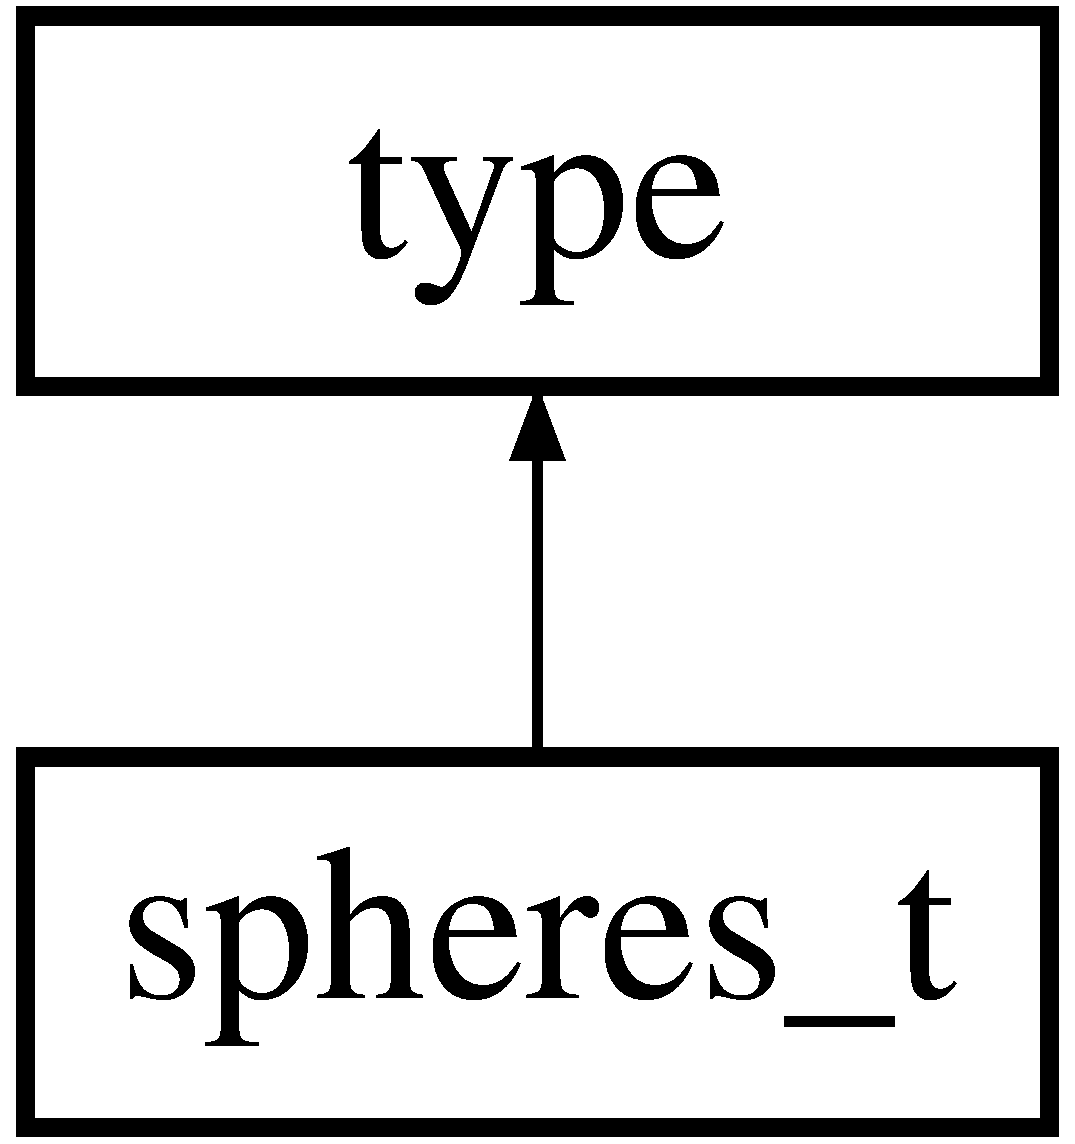
\includegraphics[height=2.000000cm]{classspheres__t}
\end{center}
\end{figure}
\subsection*{Public Types}
\begin{DoxyCompactItemize}
\item 
typedef \-::\hyperlink{classsphere__t}{sphere\-\_\-t} \hyperlink{classspheres__t_a206f1776b61d2342bf0bd21629d2a690}{sphere\-\_\-type}
\item 
typedef \\*
\-::xsd\-::cxx\-::tree\-::sequence\\*
$<$ \hyperlink{classspheres__t_a206f1776b61d2342bf0bd21629d2a690}{sphere\-\_\-type} $>$ \hyperlink{classspheres__t_ae9b4b35c1b290ab0ce8724f773d3b553}{sphere\-\_\-sequence}
\item 
typedef sphere\-\_\-sequence\-::iterator \hyperlink{classspheres__t_a9c45b4a3d0428ab6cb8e7a5d7baf06aa}{sphere\-\_\-iterator}
\item 
typedef \\*
sphere\-\_\-sequence\-::const\-\_\-iterator \hyperlink{classspheres__t_ac87f4dc7dafc3f09566e157ef3cf9985}{sphere\-\_\-const\-\_\-iterator}
\item 
typedef \\*
\-::xsd\-::cxx\-::tree\-::traits\\*
$<$ \hyperlink{classspheres__t_a206f1776b61d2342bf0bd21629d2a690}{sphere\-\_\-type}, char $>$ \hyperlink{classspheres__t_aa9e5c761af0e467b7de444613c67d826}{sphere\-\_\-traits}
\end{DoxyCompactItemize}
\subsection*{Public Member Functions}
\begin{DoxyCompactItemize}
\item 
const \hyperlink{classspheres__t_ae9b4b35c1b290ab0ce8724f773d3b553}{sphere\-\_\-sequence} \& \hyperlink{classspheres__t_a67fc4fe85acc0c7b71ebb222607e6922}{sphere} () const 
\item 
\hyperlink{classspheres__t_ae9b4b35c1b290ab0ce8724f773d3b553}{sphere\-\_\-sequence} \& \hyperlink{classspheres__t_a96c1fff53d94892c5c22e36c222735e1}{sphere} ()
\item 
void \hyperlink{classspheres__t_a798b35608f33d89d6f4cf54de932af5e}{sphere} (const \hyperlink{classspheres__t_ae9b4b35c1b290ab0ce8724f773d3b553}{sphere\-\_\-sequence} \&s)
\item 
\hyperlink{classspheres__t_a7337414c63d7510a539bcba70bba23a6}{spheres\-\_\-t} ()
\item 
\hyperlink{classspheres__t_a7110ac04fda8a3b78be4baf6ad750238}{spheres\-\_\-t} (const \-::xercesc\-::\-D\-O\-M\-Element \&e,\-::\hyperlink{namespacexml__schema_a0612287d030cb2732d31a45b258fdc87}{xml\-\_\-schema\-::flags} f=0,\-::\hyperlink{namespacexml__schema_ada9aa30dc722e93ee2ed7243085402a5}{xml\-\_\-schema\-::container} $\ast$c=0)
\item 
\hyperlink{classspheres__t_ad0379285dad67d109b42523a9a54f875}{spheres\-\_\-t} (const \hyperlink{classspheres__t}{spheres\-\_\-t} \&x,\-::\hyperlink{namespacexml__schema_a0612287d030cb2732d31a45b258fdc87}{xml\-\_\-schema\-::flags} f=0,\-::\hyperlink{namespacexml__schema_ada9aa30dc722e93ee2ed7243085402a5}{xml\-\_\-schema\-::container} $\ast$c=0)
\item 
virtual \hyperlink{classspheres__t}{spheres\-\_\-t} $\ast$ \hyperlink{classspheres__t_a0121457c1787c97cc5ac430685cb4158}{\-\_\-clone} (\-::\hyperlink{namespacexml__schema_a0612287d030cb2732d31a45b258fdc87}{xml\-\_\-schema\-::flags} f=0,\-::\hyperlink{namespacexml__schema_ada9aa30dc722e93ee2ed7243085402a5}{xml\-\_\-schema\-::container} $\ast$c=0) const 
\item 
virtual \hyperlink{classspheres__t_a92092f0b9c1862e5cfbd46d7919a8793}{$\sim$spheres\-\_\-t} ()
\end{DoxyCompactItemize}
\subsection*{Protected Member Functions}
\begin{DoxyCompactItemize}
\item 
void \hyperlink{classspheres__t_a589f664ec291de005194618d7a9cc5a2}{parse} (\-::xsd\-::cxx\-::xml\-::dom\-::parser$<$ char $>$ \&,\-::\hyperlink{namespacexml__schema_a0612287d030cb2732d31a45b258fdc87}{xml\-\_\-schema\-::flags})
\end{DoxyCompactItemize}
\subsection*{Protected Attributes}
\begin{DoxyCompactItemize}
\item 
\hyperlink{classspheres__t_ae9b4b35c1b290ab0ce8724f773d3b553}{sphere\-\_\-sequence} \hyperlink{classspheres__t_a7320f40830f4d91ea94e0ae95ccbb4e0}{sphere\-\_\-}
\end{DoxyCompactItemize}


\subsection{Member Typedef Documentation}
\hypertarget{classspheres__t_ac87f4dc7dafc3f09566e157ef3cf9985}{\index{spheres\-\_\-t@{spheres\-\_\-t}!sphere\-\_\-const\-\_\-iterator@{sphere\-\_\-const\-\_\-iterator}}
\index{sphere\-\_\-const\-\_\-iterator@{sphere\-\_\-const\-\_\-iterator}!spheres_t@{spheres\-\_\-t}}
\subsubsection[{sphere\-\_\-const\-\_\-iterator}]{\setlength{\rightskip}{0pt plus 5cm}typedef sphere\-\_\-sequence\-::const\-\_\-iterator {\bf spheres\-\_\-t\-::sphere\-\_\-const\-\_\-iterator}}}\label{classspheres__t_ac87f4dc7dafc3f09566e157ef3cf9985}
\hypertarget{classspheres__t_a9c45b4a3d0428ab6cb8e7a5d7baf06aa}{\index{spheres\-\_\-t@{spheres\-\_\-t}!sphere\-\_\-iterator@{sphere\-\_\-iterator}}
\index{sphere\-\_\-iterator@{sphere\-\_\-iterator}!spheres_t@{spheres\-\_\-t}}
\subsubsection[{sphere\-\_\-iterator}]{\setlength{\rightskip}{0pt plus 5cm}typedef sphere\-\_\-sequence\-::iterator {\bf spheres\-\_\-t\-::sphere\-\_\-iterator}}}\label{classspheres__t_a9c45b4a3d0428ab6cb8e7a5d7baf06aa}
\hypertarget{classspheres__t_ae9b4b35c1b290ab0ce8724f773d3b553}{\index{spheres\-\_\-t@{spheres\-\_\-t}!sphere\-\_\-sequence@{sphere\-\_\-sequence}}
\index{sphere\-\_\-sequence@{sphere\-\_\-sequence}!spheres_t@{spheres\-\_\-t}}
\subsubsection[{sphere\-\_\-sequence}]{\setlength{\rightskip}{0pt plus 5cm}typedef \-::xsd\-::cxx\-::tree\-::sequence$<$ {\bf sphere\-\_\-type} $>$ {\bf spheres\-\_\-t\-::sphere\-\_\-sequence}}}\label{classspheres__t_ae9b4b35c1b290ab0ce8724f773d3b553}
\hypertarget{classspheres__t_aa9e5c761af0e467b7de444613c67d826}{\index{spheres\-\_\-t@{spheres\-\_\-t}!sphere\-\_\-traits@{sphere\-\_\-traits}}
\index{sphere\-\_\-traits@{sphere\-\_\-traits}!spheres_t@{spheres\-\_\-t}}
\subsubsection[{sphere\-\_\-traits}]{\setlength{\rightskip}{0pt plus 5cm}typedef \-::xsd\-::cxx\-::tree\-::traits$<$ {\bf sphere\-\_\-type}, char $>$ {\bf spheres\-\_\-t\-::sphere\-\_\-traits}}}\label{classspheres__t_aa9e5c761af0e467b7de444613c67d826}
\hypertarget{classspheres__t_a206f1776b61d2342bf0bd21629d2a690}{\index{spheres\-\_\-t@{spheres\-\_\-t}!sphere\-\_\-type@{sphere\-\_\-type}}
\index{sphere\-\_\-type@{sphere\-\_\-type}!spheres_t@{spheres\-\_\-t}}
\subsubsection[{sphere\-\_\-type}]{\setlength{\rightskip}{0pt plus 5cm}typedef \-::{\bf sphere\-\_\-t} {\bf spheres\-\_\-t\-::sphere\-\_\-type}}}\label{classspheres__t_a206f1776b61d2342bf0bd21629d2a690}


\subsection{Constructor \& Destructor Documentation}
\hypertarget{classspheres__t_a7337414c63d7510a539bcba70bba23a6}{\index{spheres\-\_\-t@{spheres\-\_\-t}!spheres\-\_\-t@{spheres\-\_\-t}}
\index{spheres\-\_\-t@{spheres\-\_\-t}!spheres_t@{spheres\-\_\-t}}
\subsubsection[{spheres\-\_\-t}]{\setlength{\rightskip}{0pt plus 5cm}spheres\-\_\-t\-::spheres\-\_\-t (
\begin{DoxyParamCaption}
{}
\end{DoxyParamCaption}
)}}\label{classspheres__t_a7337414c63d7510a539bcba70bba23a6}
\hypertarget{classspheres__t_a7110ac04fda8a3b78be4baf6ad750238}{\index{spheres\-\_\-t@{spheres\-\_\-t}!spheres\-\_\-t@{spheres\-\_\-t}}
\index{spheres\-\_\-t@{spheres\-\_\-t}!spheres_t@{spheres\-\_\-t}}
\subsubsection[{spheres\-\_\-t}]{\setlength{\rightskip}{0pt plus 5cm}spheres\-\_\-t\-::spheres\-\_\-t (
\begin{DoxyParamCaption}
\item[{const \-::xercesc\-::\-D\-O\-M\-Element \&}]{e, }
\item[{\-::{\bf xml\-\_\-schema\-::flags}}]{f = {\ttfamily 0}, }
\item[{\-::{\bf xml\-\_\-schema\-::container} $\ast$}]{c = {\ttfamily 0}}
\end{DoxyParamCaption}
)}}\label{classspheres__t_a7110ac04fda8a3b78be4baf6ad750238}
\hypertarget{classspheres__t_ad0379285dad67d109b42523a9a54f875}{\index{spheres\-\_\-t@{spheres\-\_\-t}!spheres\-\_\-t@{spheres\-\_\-t}}
\index{spheres\-\_\-t@{spheres\-\_\-t}!spheres_t@{spheres\-\_\-t}}
\subsubsection[{spheres\-\_\-t}]{\setlength{\rightskip}{0pt plus 5cm}spheres\-\_\-t\-::spheres\-\_\-t (
\begin{DoxyParamCaption}
\item[{const {\bf spheres\-\_\-t} \&}]{x, }
\item[{\-::{\bf xml\-\_\-schema\-::flags}}]{f = {\ttfamily 0}, }
\item[{\-::{\bf xml\-\_\-schema\-::container} $\ast$}]{c = {\ttfamily 0}}
\end{DoxyParamCaption}
)}}\label{classspheres__t_ad0379285dad67d109b42523a9a54f875}
\hypertarget{classspheres__t_a92092f0b9c1862e5cfbd46d7919a8793}{\index{spheres\-\_\-t@{spheres\-\_\-t}!$\sim$spheres\-\_\-t@{$\sim$spheres\-\_\-t}}
\index{$\sim$spheres\-\_\-t@{$\sim$spheres\-\_\-t}!spheres_t@{spheres\-\_\-t}}
\subsubsection[{$\sim$spheres\-\_\-t}]{\setlength{\rightskip}{0pt plus 5cm}spheres\-\_\-t\-::$\sim$spheres\-\_\-t (
\begin{DoxyParamCaption}
{}
\end{DoxyParamCaption}
)\hspace{0.3cm}{\ttfamily [virtual]}}}\label{classspheres__t_a92092f0b9c1862e5cfbd46d7919a8793}


\subsection{Member Function Documentation}
\hypertarget{classspheres__t_a0121457c1787c97cc5ac430685cb4158}{\index{spheres\-\_\-t@{spheres\-\_\-t}!\-\_\-clone@{\-\_\-clone}}
\index{\-\_\-clone@{\-\_\-clone}!spheres_t@{spheres\-\_\-t}}
\subsubsection[{\-\_\-clone}]{\setlength{\rightskip}{0pt plus 5cm}{\bf spheres\-\_\-t} $\ast$ spheres\-\_\-t\-::\-\_\-clone (
\begin{DoxyParamCaption}
\item[{\-::{\bf xml\-\_\-schema\-::flags}}]{f = {\ttfamily 0}, }
\item[{\-::{\bf xml\-\_\-schema\-::container} $\ast$}]{c = {\ttfamily 0}}
\end{DoxyParamCaption}
) const\hspace{0.3cm}{\ttfamily [virtual]}}}\label{classspheres__t_a0121457c1787c97cc5ac430685cb4158}
\hypertarget{classspheres__t_a589f664ec291de005194618d7a9cc5a2}{\index{spheres\-\_\-t@{spheres\-\_\-t}!parse@{parse}}
\index{parse@{parse}!spheres_t@{spheres\-\_\-t}}
\subsubsection[{parse}]{\setlength{\rightskip}{0pt plus 5cm}void spheres\-\_\-t\-::parse (
\begin{DoxyParamCaption}
\item[{\-::xsd\-::cxx\-::xml\-::dom\-::parser$<$ char $>$ \&}]{p, }
\item[{\-::{\bf xml\-\_\-schema\-::flags}}]{f}
\end{DoxyParamCaption}
)\hspace{0.3cm}{\ttfamily [protected]}}}\label{classspheres__t_a589f664ec291de005194618d7a9cc5a2}
\hypertarget{classspheres__t_a67fc4fe85acc0c7b71ebb222607e6922}{\index{spheres\-\_\-t@{spheres\-\_\-t}!sphere@{sphere}}
\index{sphere@{sphere}!spheres_t@{spheres\-\_\-t}}
\subsubsection[{sphere}]{\setlength{\rightskip}{0pt plus 5cm}const {\bf spheres\-\_\-t\-::sphere\-\_\-sequence} \& spheres\-\_\-t\-::sphere (
\begin{DoxyParamCaption}
{}
\end{DoxyParamCaption}
) const}}\label{classspheres__t_a67fc4fe85acc0c7b71ebb222607e6922}
\hypertarget{classspheres__t_a96c1fff53d94892c5c22e36c222735e1}{\index{spheres\-\_\-t@{spheres\-\_\-t}!sphere@{sphere}}
\index{sphere@{sphere}!spheres_t@{spheres\-\_\-t}}
\subsubsection[{sphere}]{\setlength{\rightskip}{0pt plus 5cm}{\bf spheres\-\_\-t\-::sphere\-\_\-sequence} \& spheres\-\_\-t\-::sphere (
\begin{DoxyParamCaption}
{}
\end{DoxyParamCaption}
)}}\label{classspheres__t_a96c1fff53d94892c5c22e36c222735e1}
\hypertarget{classspheres__t_a798b35608f33d89d6f4cf54de932af5e}{\index{spheres\-\_\-t@{spheres\-\_\-t}!sphere@{sphere}}
\index{sphere@{sphere}!spheres_t@{spheres\-\_\-t}}
\subsubsection[{sphere}]{\setlength{\rightskip}{0pt plus 5cm}void spheres\-\_\-t\-::sphere (
\begin{DoxyParamCaption}
\item[{const {\bf sphere\-\_\-sequence} \&}]{s}
\end{DoxyParamCaption}
)}}\label{classspheres__t_a798b35608f33d89d6f4cf54de932af5e}


\subsection{Member Data Documentation}
\hypertarget{classspheres__t_a7320f40830f4d91ea94e0ae95ccbb4e0}{\index{spheres\-\_\-t@{spheres\-\_\-t}!sphere\-\_\-@{sphere\-\_\-}}
\index{sphere\-\_\-@{sphere\-\_\-}!spheres_t@{spheres\-\_\-t}}
\subsubsection[{sphere\-\_\-}]{\setlength{\rightskip}{0pt plus 5cm}{\bf sphere\-\_\-sequence} spheres\-\_\-t\-::sphere\-\_\-\hspace{0.3cm}{\ttfamily [protected]}}}\label{classspheres__t_a7320f40830f4d91ea94e0ae95ccbb4e0}


The documentation for this class was generated from the following files\-:\begin{DoxyCompactItemize}
\item 
src/utils/\hyperlink{InputSpheres_8h}{Input\-Spheres.\-h}\item 
src/utils/\hyperlink{InputSpheres_8cpp}{Input\-Spheres.\-cpp}\end{DoxyCompactItemize}

\hypertarget{classstartV__t}{\section{start\-V\-\_\-t Class Reference}
\label{classstartV__t}\index{start\-V\-\_\-t@{start\-V\-\_\-t}}
}


{\ttfamily \#include $<$Input\-Cuboids.\-h$>$}

Inheritance diagram for start\-V\-\_\-t\-:\begin{figure}[H]
\begin{center}
\leavevmode
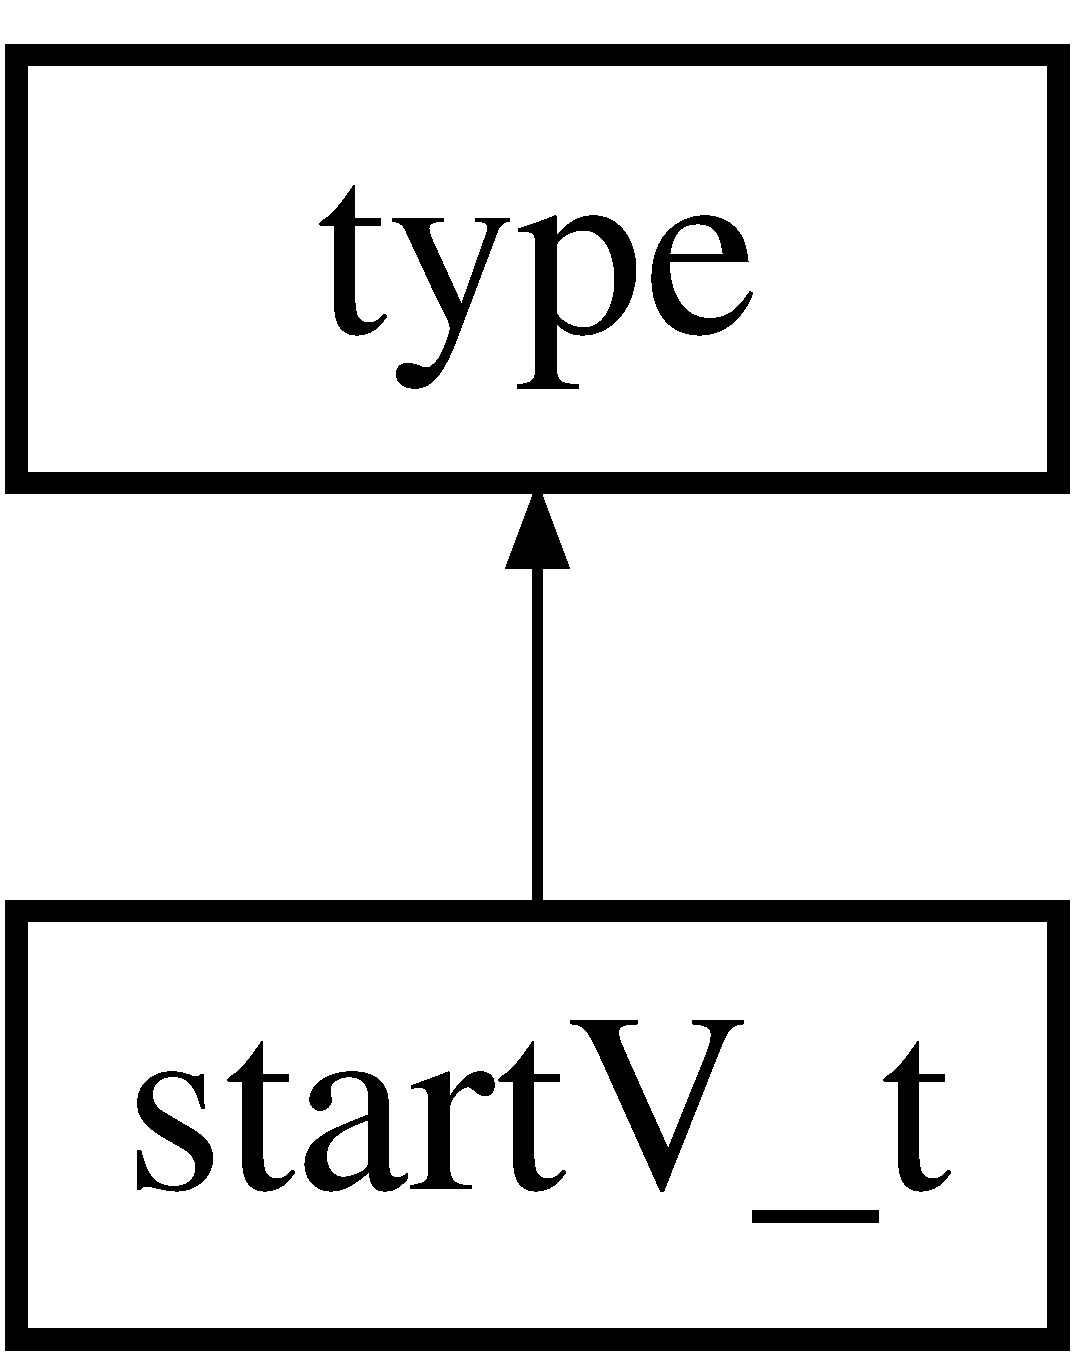
\includegraphics[height=2.000000cm]{classstartV__t}
\end{center}
\end{figure}
\subsection*{Public Types}
\begin{DoxyCompactItemize}
\item 
typedef \-::\hyperlink{namespacexml__schema_a69bfaf24f63a8c18ebd8e21db6b343df}{xml\-\_\-schema\-::decimal} \hyperlink{classstartV__t_aac8a2d74e6be7ae3248ba26d253ad3fc}{vel\-X\-\_\-type}
\item 
typedef \\*
\-::xsd\-::cxx\-::tree\-::traits\\*
$<$ \hyperlink{classstartV__t_aac8a2d74e6be7ae3248ba26d253ad3fc}{vel\-X\-\_\-type}, char,\-::xsd\-::cxx\-::tree\-::schema\-\_\-type\-::decimal $>$ \hyperlink{classstartV__t_aee57fb6e5210e3f5cdb037863d901086}{vel\-X\-\_\-traits}
\item 
typedef \-::\hyperlink{namespacexml__schema_a69bfaf24f63a8c18ebd8e21db6b343df}{xml\-\_\-schema\-::decimal} \hyperlink{classstartV__t_acfa8dd01ff687d610335845945099743}{vel\-Y\-\_\-type}
\item 
typedef \\*
\-::xsd\-::cxx\-::tree\-::traits\\*
$<$ \hyperlink{classstartV__t_acfa8dd01ff687d610335845945099743}{vel\-Y\-\_\-type}, char,\-::xsd\-::cxx\-::tree\-::schema\-\_\-type\-::decimal $>$ \hyperlink{classstartV__t_a004e9fe52571fa7204d075feb71c244e}{vel\-Y\-\_\-traits}
\item 
typedef \-::\hyperlink{namespacexml__schema_a69bfaf24f63a8c18ebd8e21db6b343df}{xml\-\_\-schema\-::decimal} \hyperlink{classstartV__t_ae49f578f0cc0d86f126691188752dfe9}{vel\-Z\-\_\-type}
\item 
typedef \\*
\-::xsd\-::cxx\-::tree\-::traits\\*
$<$ \hyperlink{classstartV__t_ae49f578f0cc0d86f126691188752dfe9}{vel\-Z\-\_\-type}, char,\-::xsd\-::cxx\-::tree\-::schema\-\_\-type\-::decimal $>$ \hyperlink{classstartV__t_ab8922309ab467a161007402cf39c89e5}{vel\-Z\-\_\-traits}
\end{DoxyCompactItemize}
\subsection*{Public Member Functions}
\begin{DoxyCompactItemize}
\item 
const \hyperlink{classstartV__t_aac8a2d74e6be7ae3248ba26d253ad3fc}{vel\-X\-\_\-type} \& \hyperlink{classstartV__t_a4340410f0380ecb35db2eafb18c5fee9}{vel\-X} () const 
\item 
\hyperlink{classstartV__t_aac8a2d74e6be7ae3248ba26d253ad3fc}{vel\-X\-\_\-type} \& \hyperlink{classstartV__t_abaf0997273c09b09572e39e3976f676d}{vel\-X} ()
\item 
void \hyperlink{classstartV__t_a9fa96a1a14b2414de3a69ad945aaf35a}{vel\-X} (const \hyperlink{classstartV__t_aac8a2d74e6be7ae3248ba26d253ad3fc}{vel\-X\-\_\-type} \&x)
\item 
const \hyperlink{classstartV__t_acfa8dd01ff687d610335845945099743}{vel\-Y\-\_\-type} \& \hyperlink{classstartV__t_a0c066d13b456db18bf5306e996e43c07}{vel\-Y} () const 
\item 
\hyperlink{classstartV__t_acfa8dd01ff687d610335845945099743}{vel\-Y\-\_\-type} \& \hyperlink{classstartV__t_a0603b086828b9023554f54ac4a071ead}{vel\-Y} ()
\item 
void \hyperlink{classstartV__t_a1e0a243dc357bd088644e62a81a59f83}{vel\-Y} (const \hyperlink{classstartV__t_acfa8dd01ff687d610335845945099743}{vel\-Y\-\_\-type} \&x)
\item 
const \hyperlink{classstartV__t_ae49f578f0cc0d86f126691188752dfe9}{vel\-Z\-\_\-type} \& \hyperlink{classstartV__t_aba04ae5938c29de72436ed303c3809bd}{vel\-Z} () const 
\item 
\hyperlink{classstartV__t_ae49f578f0cc0d86f126691188752dfe9}{vel\-Z\-\_\-type} \& \hyperlink{classstartV__t_a823df50569f539fc5c285f3879577428}{vel\-Z} ()
\item 
void \hyperlink{classstartV__t_a0b8d6e20780d58af86ce99977de5933a}{vel\-Z} (const \hyperlink{classstartV__t_ae49f578f0cc0d86f126691188752dfe9}{vel\-Z\-\_\-type} \&x)
\item 
\hyperlink{classstartV__t_a399904b82739e84b0e9dced2ee2f7590}{start\-V\-\_\-t} (const \hyperlink{classstartV__t_aac8a2d74e6be7ae3248ba26d253ad3fc}{vel\-X\-\_\-type} \&, const \hyperlink{classstartV__t_acfa8dd01ff687d610335845945099743}{vel\-Y\-\_\-type} \&, const \hyperlink{classstartV__t_ae49f578f0cc0d86f126691188752dfe9}{vel\-Z\-\_\-type} \&)
\item 
\hyperlink{classstartV__t_aba4d6f5c9f7209e5909278629e3c2229}{start\-V\-\_\-t} (const \-::xercesc\-::\-D\-O\-M\-Element \&e,\-::\hyperlink{namespacexml__schema_a0612287d030cb2732d31a45b258fdc87}{xml\-\_\-schema\-::flags} f=0,\-::\hyperlink{namespacexml__schema_ada9aa30dc722e93ee2ed7243085402a5}{xml\-\_\-schema\-::container} $\ast$c=0)
\item 
\hyperlink{classstartV__t_af6ca7294009d489477fa5d76f15254f3}{start\-V\-\_\-t} (const \hyperlink{classstartV__t}{start\-V\-\_\-t} \&x,\-::\hyperlink{namespacexml__schema_a0612287d030cb2732d31a45b258fdc87}{xml\-\_\-schema\-::flags} f=0,\-::\hyperlink{namespacexml__schema_ada9aa30dc722e93ee2ed7243085402a5}{xml\-\_\-schema\-::container} $\ast$c=0)
\item 
virtual \hyperlink{classstartV__t}{start\-V\-\_\-t} $\ast$ \hyperlink{classstartV__t_aa4a126b38cc99822434689c9ee5bf475}{\-\_\-clone} (\-::\hyperlink{namespacexml__schema_a0612287d030cb2732d31a45b258fdc87}{xml\-\_\-schema\-::flags} f=0,\-::\hyperlink{namespacexml__schema_ada9aa30dc722e93ee2ed7243085402a5}{xml\-\_\-schema\-::container} $\ast$c=0) const 
\item 
virtual \hyperlink{classstartV__t_af4c2e25f679f941f94136709ca0d2152}{$\sim$start\-V\-\_\-t} ()
\end{DoxyCompactItemize}
\subsection*{Protected Member Functions}
\begin{DoxyCompactItemize}
\item 
void \hyperlink{classstartV__t_ad78656f3c8c3d04eb97f6d6796185edc}{parse} (\-::xsd\-::cxx\-::xml\-::dom\-::parser$<$ char $>$ \&,\-::\hyperlink{namespacexml__schema_a0612287d030cb2732d31a45b258fdc87}{xml\-\_\-schema\-::flags})
\end{DoxyCompactItemize}
\subsection*{Protected Attributes}
\begin{DoxyCompactItemize}
\item 
\-::xsd\-::cxx\-::tree\-::one$<$ \hyperlink{classstartV__t_aac8a2d74e6be7ae3248ba26d253ad3fc}{vel\-X\-\_\-type} $>$ \hyperlink{classstartV__t_a0d6673157cfcb402a50d54345e1a8312}{vel\-X\-\_\-}
\item 
\-::xsd\-::cxx\-::tree\-::one$<$ \hyperlink{classstartV__t_acfa8dd01ff687d610335845945099743}{vel\-Y\-\_\-type} $>$ \hyperlink{classstartV__t_ad4eb49113a9009d4834ab3cc2cb3dca3}{vel\-Y\-\_\-}
\item 
\-::xsd\-::cxx\-::tree\-::one$<$ \hyperlink{classstartV__t_ae49f578f0cc0d86f126691188752dfe9}{vel\-Z\-\_\-type} $>$ \hyperlink{classstartV__t_a8069b315d8ad335b23e90f42c94fb3a8}{vel\-Z\-\_\-}
\end{DoxyCompactItemize}


\subsection{Member Typedef Documentation}
\hypertarget{classstartV__t_aee57fb6e5210e3f5cdb037863d901086}{\index{start\-V\-\_\-t@{start\-V\-\_\-t}!vel\-X\-\_\-traits@{vel\-X\-\_\-traits}}
\index{vel\-X\-\_\-traits@{vel\-X\-\_\-traits}!startV_t@{start\-V\-\_\-t}}
\subsubsection[{vel\-X\-\_\-traits}]{\setlength{\rightskip}{0pt plus 5cm}typedef \-::xsd\-::cxx\-::tree\-::traits$<$ {\bf vel\-X\-\_\-type}, char, \-::xsd\-::cxx\-::tree\-::schema\-\_\-type\-::decimal $>$ {\bf start\-V\-\_\-t\-::vel\-X\-\_\-traits}}}\label{classstartV__t_aee57fb6e5210e3f5cdb037863d901086}
\hypertarget{classstartV__t_aac8a2d74e6be7ae3248ba26d253ad3fc}{\index{start\-V\-\_\-t@{start\-V\-\_\-t}!vel\-X\-\_\-type@{vel\-X\-\_\-type}}
\index{vel\-X\-\_\-type@{vel\-X\-\_\-type}!startV_t@{start\-V\-\_\-t}}
\subsubsection[{vel\-X\-\_\-type}]{\setlength{\rightskip}{0pt plus 5cm}typedef \-::{\bf xml\-\_\-schema\-::decimal} {\bf start\-V\-\_\-t\-::vel\-X\-\_\-type}}}\label{classstartV__t_aac8a2d74e6be7ae3248ba26d253ad3fc}
\hypertarget{classstartV__t_a004e9fe52571fa7204d075feb71c244e}{\index{start\-V\-\_\-t@{start\-V\-\_\-t}!vel\-Y\-\_\-traits@{vel\-Y\-\_\-traits}}
\index{vel\-Y\-\_\-traits@{vel\-Y\-\_\-traits}!startV_t@{start\-V\-\_\-t}}
\subsubsection[{vel\-Y\-\_\-traits}]{\setlength{\rightskip}{0pt plus 5cm}typedef \-::xsd\-::cxx\-::tree\-::traits$<$ {\bf vel\-Y\-\_\-type}, char, \-::xsd\-::cxx\-::tree\-::schema\-\_\-type\-::decimal $>$ {\bf start\-V\-\_\-t\-::vel\-Y\-\_\-traits}}}\label{classstartV__t_a004e9fe52571fa7204d075feb71c244e}
\hypertarget{classstartV__t_acfa8dd01ff687d610335845945099743}{\index{start\-V\-\_\-t@{start\-V\-\_\-t}!vel\-Y\-\_\-type@{vel\-Y\-\_\-type}}
\index{vel\-Y\-\_\-type@{vel\-Y\-\_\-type}!startV_t@{start\-V\-\_\-t}}
\subsubsection[{vel\-Y\-\_\-type}]{\setlength{\rightskip}{0pt plus 5cm}typedef \-::{\bf xml\-\_\-schema\-::decimal} {\bf start\-V\-\_\-t\-::vel\-Y\-\_\-type}}}\label{classstartV__t_acfa8dd01ff687d610335845945099743}
\hypertarget{classstartV__t_ab8922309ab467a161007402cf39c89e5}{\index{start\-V\-\_\-t@{start\-V\-\_\-t}!vel\-Z\-\_\-traits@{vel\-Z\-\_\-traits}}
\index{vel\-Z\-\_\-traits@{vel\-Z\-\_\-traits}!startV_t@{start\-V\-\_\-t}}
\subsubsection[{vel\-Z\-\_\-traits}]{\setlength{\rightskip}{0pt plus 5cm}typedef \-::xsd\-::cxx\-::tree\-::traits$<$ {\bf vel\-Z\-\_\-type}, char, \-::xsd\-::cxx\-::tree\-::schema\-\_\-type\-::decimal $>$ {\bf start\-V\-\_\-t\-::vel\-Z\-\_\-traits}}}\label{classstartV__t_ab8922309ab467a161007402cf39c89e5}
\hypertarget{classstartV__t_ae49f578f0cc0d86f126691188752dfe9}{\index{start\-V\-\_\-t@{start\-V\-\_\-t}!vel\-Z\-\_\-type@{vel\-Z\-\_\-type}}
\index{vel\-Z\-\_\-type@{vel\-Z\-\_\-type}!startV_t@{start\-V\-\_\-t}}
\subsubsection[{vel\-Z\-\_\-type}]{\setlength{\rightskip}{0pt plus 5cm}typedef \-::{\bf xml\-\_\-schema\-::decimal} {\bf start\-V\-\_\-t\-::vel\-Z\-\_\-type}}}\label{classstartV__t_ae49f578f0cc0d86f126691188752dfe9}


\subsection{Constructor \& Destructor Documentation}
\hypertarget{classstartV__t_a399904b82739e84b0e9dced2ee2f7590}{\index{start\-V\-\_\-t@{start\-V\-\_\-t}!start\-V\-\_\-t@{start\-V\-\_\-t}}
\index{start\-V\-\_\-t@{start\-V\-\_\-t}!startV_t@{start\-V\-\_\-t}}
\subsubsection[{start\-V\-\_\-t}]{\setlength{\rightskip}{0pt plus 5cm}start\-V\-\_\-t\-::start\-V\-\_\-t (
\begin{DoxyParamCaption}
\item[{const {\bf vel\-X\-\_\-type} \&}]{vel\-X, }
\item[{const {\bf vel\-Y\-\_\-type} \&}]{vel\-Y, }
\item[{const {\bf vel\-Z\-\_\-type} \&}]{vel\-Z}
\end{DoxyParamCaption}
)}}\label{classstartV__t_a399904b82739e84b0e9dced2ee2f7590}
\hypertarget{classstartV__t_aba4d6f5c9f7209e5909278629e3c2229}{\index{start\-V\-\_\-t@{start\-V\-\_\-t}!start\-V\-\_\-t@{start\-V\-\_\-t}}
\index{start\-V\-\_\-t@{start\-V\-\_\-t}!startV_t@{start\-V\-\_\-t}}
\subsubsection[{start\-V\-\_\-t}]{\setlength{\rightskip}{0pt plus 5cm}start\-V\-\_\-t\-::start\-V\-\_\-t (
\begin{DoxyParamCaption}
\item[{const \-::xercesc\-::\-D\-O\-M\-Element \&}]{e, }
\item[{\-::{\bf xml\-\_\-schema\-::flags}}]{f = {\ttfamily 0}, }
\item[{\-::{\bf xml\-\_\-schema\-::container} $\ast$}]{c = {\ttfamily 0}}
\end{DoxyParamCaption}
)}}\label{classstartV__t_aba4d6f5c9f7209e5909278629e3c2229}
\hypertarget{classstartV__t_af6ca7294009d489477fa5d76f15254f3}{\index{start\-V\-\_\-t@{start\-V\-\_\-t}!start\-V\-\_\-t@{start\-V\-\_\-t}}
\index{start\-V\-\_\-t@{start\-V\-\_\-t}!startV_t@{start\-V\-\_\-t}}
\subsubsection[{start\-V\-\_\-t}]{\setlength{\rightskip}{0pt plus 5cm}start\-V\-\_\-t\-::start\-V\-\_\-t (
\begin{DoxyParamCaption}
\item[{const {\bf start\-V\-\_\-t} \&}]{x, }
\item[{\-::{\bf xml\-\_\-schema\-::flags}}]{f = {\ttfamily 0}, }
\item[{\-::{\bf xml\-\_\-schema\-::container} $\ast$}]{c = {\ttfamily 0}}
\end{DoxyParamCaption}
)}}\label{classstartV__t_af6ca7294009d489477fa5d76f15254f3}
\hypertarget{classstartV__t_af4c2e25f679f941f94136709ca0d2152}{\index{start\-V\-\_\-t@{start\-V\-\_\-t}!$\sim$start\-V\-\_\-t@{$\sim$start\-V\-\_\-t}}
\index{$\sim$start\-V\-\_\-t@{$\sim$start\-V\-\_\-t}!startV_t@{start\-V\-\_\-t}}
\subsubsection[{$\sim$start\-V\-\_\-t}]{\setlength{\rightskip}{0pt plus 5cm}start\-V\-\_\-t\-::$\sim$start\-V\-\_\-t (
\begin{DoxyParamCaption}
{}
\end{DoxyParamCaption}
)\hspace{0.3cm}{\ttfamily [virtual]}}}\label{classstartV__t_af4c2e25f679f941f94136709ca0d2152}


\subsection{Member Function Documentation}
\hypertarget{classstartV__t_aa4a126b38cc99822434689c9ee5bf475}{\index{start\-V\-\_\-t@{start\-V\-\_\-t}!\-\_\-clone@{\-\_\-clone}}
\index{\-\_\-clone@{\-\_\-clone}!startV_t@{start\-V\-\_\-t}}
\subsubsection[{\-\_\-clone}]{\setlength{\rightskip}{0pt plus 5cm}{\bf start\-V\-\_\-t} $\ast$ start\-V\-\_\-t\-::\-\_\-clone (
\begin{DoxyParamCaption}
\item[{\-::{\bf xml\-\_\-schema\-::flags}}]{f = {\ttfamily 0}, }
\item[{\-::{\bf xml\-\_\-schema\-::container} $\ast$}]{c = {\ttfamily 0}}
\end{DoxyParamCaption}
) const\hspace{0.3cm}{\ttfamily [virtual]}}}\label{classstartV__t_aa4a126b38cc99822434689c9ee5bf475}
\hypertarget{classstartV__t_ad78656f3c8c3d04eb97f6d6796185edc}{\index{start\-V\-\_\-t@{start\-V\-\_\-t}!parse@{parse}}
\index{parse@{parse}!startV_t@{start\-V\-\_\-t}}
\subsubsection[{parse}]{\setlength{\rightskip}{0pt plus 5cm}void start\-V\-\_\-t\-::parse (
\begin{DoxyParamCaption}
\item[{\-::xsd\-::cxx\-::xml\-::dom\-::parser$<$ char $>$ \&}]{p, }
\item[{\-::{\bf xml\-\_\-schema\-::flags}}]{f}
\end{DoxyParamCaption}
)\hspace{0.3cm}{\ttfamily [protected]}}}\label{classstartV__t_ad78656f3c8c3d04eb97f6d6796185edc}
\hypertarget{classstartV__t_a4340410f0380ecb35db2eafb18c5fee9}{\index{start\-V\-\_\-t@{start\-V\-\_\-t}!vel\-X@{vel\-X}}
\index{vel\-X@{vel\-X}!startV_t@{start\-V\-\_\-t}}
\subsubsection[{vel\-X}]{\setlength{\rightskip}{0pt plus 5cm}const {\bf start\-V\-\_\-t\-::vel\-X\-\_\-type} \& start\-V\-\_\-t\-::vel\-X (
\begin{DoxyParamCaption}
{}
\end{DoxyParamCaption}
) const}}\label{classstartV__t_a4340410f0380ecb35db2eafb18c5fee9}
\hypertarget{classstartV__t_abaf0997273c09b09572e39e3976f676d}{\index{start\-V\-\_\-t@{start\-V\-\_\-t}!vel\-X@{vel\-X}}
\index{vel\-X@{vel\-X}!startV_t@{start\-V\-\_\-t}}
\subsubsection[{vel\-X}]{\setlength{\rightskip}{0pt plus 5cm}{\bf start\-V\-\_\-t\-::vel\-X\-\_\-type} \& start\-V\-\_\-t\-::vel\-X (
\begin{DoxyParamCaption}
{}
\end{DoxyParamCaption}
)}}\label{classstartV__t_abaf0997273c09b09572e39e3976f676d}
\hypertarget{classstartV__t_a9fa96a1a14b2414de3a69ad945aaf35a}{\index{start\-V\-\_\-t@{start\-V\-\_\-t}!vel\-X@{vel\-X}}
\index{vel\-X@{vel\-X}!startV_t@{start\-V\-\_\-t}}
\subsubsection[{vel\-X}]{\setlength{\rightskip}{0pt plus 5cm}void start\-V\-\_\-t\-::vel\-X (
\begin{DoxyParamCaption}
\item[{const {\bf vel\-X\-\_\-type} \&}]{x}
\end{DoxyParamCaption}
)}}\label{classstartV__t_a9fa96a1a14b2414de3a69ad945aaf35a}
\hypertarget{classstartV__t_a0c066d13b456db18bf5306e996e43c07}{\index{start\-V\-\_\-t@{start\-V\-\_\-t}!vel\-Y@{vel\-Y}}
\index{vel\-Y@{vel\-Y}!startV_t@{start\-V\-\_\-t}}
\subsubsection[{vel\-Y}]{\setlength{\rightskip}{0pt plus 5cm}const {\bf start\-V\-\_\-t\-::vel\-Y\-\_\-type} \& start\-V\-\_\-t\-::vel\-Y (
\begin{DoxyParamCaption}
{}
\end{DoxyParamCaption}
) const}}\label{classstartV__t_a0c066d13b456db18bf5306e996e43c07}
\hypertarget{classstartV__t_a0603b086828b9023554f54ac4a071ead}{\index{start\-V\-\_\-t@{start\-V\-\_\-t}!vel\-Y@{vel\-Y}}
\index{vel\-Y@{vel\-Y}!startV_t@{start\-V\-\_\-t}}
\subsubsection[{vel\-Y}]{\setlength{\rightskip}{0pt plus 5cm}{\bf start\-V\-\_\-t\-::vel\-Y\-\_\-type} \& start\-V\-\_\-t\-::vel\-Y (
\begin{DoxyParamCaption}
{}
\end{DoxyParamCaption}
)}}\label{classstartV__t_a0603b086828b9023554f54ac4a071ead}
\hypertarget{classstartV__t_a1e0a243dc357bd088644e62a81a59f83}{\index{start\-V\-\_\-t@{start\-V\-\_\-t}!vel\-Y@{vel\-Y}}
\index{vel\-Y@{vel\-Y}!startV_t@{start\-V\-\_\-t}}
\subsubsection[{vel\-Y}]{\setlength{\rightskip}{0pt plus 5cm}void start\-V\-\_\-t\-::vel\-Y (
\begin{DoxyParamCaption}
\item[{const {\bf vel\-Y\-\_\-type} \&}]{x}
\end{DoxyParamCaption}
)}}\label{classstartV__t_a1e0a243dc357bd088644e62a81a59f83}
\hypertarget{classstartV__t_aba04ae5938c29de72436ed303c3809bd}{\index{start\-V\-\_\-t@{start\-V\-\_\-t}!vel\-Z@{vel\-Z}}
\index{vel\-Z@{vel\-Z}!startV_t@{start\-V\-\_\-t}}
\subsubsection[{vel\-Z}]{\setlength{\rightskip}{0pt plus 5cm}const {\bf start\-V\-\_\-t\-::vel\-Z\-\_\-type} \& start\-V\-\_\-t\-::vel\-Z (
\begin{DoxyParamCaption}
{}
\end{DoxyParamCaption}
) const}}\label{classstartV__t_aba04ae5938c29de72436ed303c3809bd}
\hypertarget{classstartV__t_a823df50569f539fc5c285f3879577428}{\index{start\-V\-\_\-t@{start\-V\-\_\-t}!vel\-Z@{vel\-Z}}
\index{vel\-Z@{vel\-Z}!startV_t@{start\-V\-\_\-t}}
\subsubsection[{vel\-Z}]{\setlength{\rightskip}{0pt plus 5cm}{\bf start\-V\-\_\-t\-::vel\-Z\-\_\-type} \& start\-V\-\_\-t\-::vel\-Z (
\begin{DoxyParamCaption}
{}
\end{DoxyParamCaption}
)}}\label{classstartV__t_a823df50569f539fc5c285f3879577428}
\hypertarget{classstartV__t_a0b8d6e20780d58af86ce99977de5933a}{\index{start\-V\-\_\-t@{start\-V\-\_\-t}!vel\-Z@{vel\-Z}}
\index{vel\-Z@{vel\-Z}!startV_t@{start\-V\-\_\-t}}
\subsubsection[{vel\-Z}]{\setlength{\rightskip}{0pt plus 5cm}void start\-V\-\_\-t\-::vel\-Z (
\begin{DoxyParamCaption}
\item[{const {\bf vel\-Z\-\_\-type} \&}]{x}
\end{DoxyParamCaption}
)}}\label{classstartV__t_a0b8d6e20780d58af86ce99977de5933a}


\subsection{Member Data Documentation}
\hypertarget{classstartV__t_a0d6673157cfcb402a50d54345e1a8312}{\index{start\-V\-\_\-t@{start\-V\-\_\-t}!vel\-X\-\_\-@{vel\-X\-\_\-}}
\index{vel\-X\-\_\-@{vel\-X\-\_\-}!startV_t@{start\-V\-\_\-t}}
\subsubsection[{vel\-X\-\_\-}]{\setlength{\rightskip}{0pt plus 5cm}\-::xsd\-::cxx\-::tree\-::one$<$ {\bf vel\-X\-\_\-type} $>$ start\-V\-\_\-t\-::vel\-X\-\_\-\hspace{0.3cm}{\ttfamily [protected]}}}\label{classstartV__t_a0d6673157cfcb402a50d54345e1a8312}
\hypertarget{classstartV__t_ad4eb49113a9009d4834ab3cc2cb3dca3}{\index{start\-V\-\_\-t@{start\-V\-\_\-t}!vel\-Y\-\_\-@{vel\-Y\-\_\-}}
\index{vel\-Y\-\_\-@{vel\-Y\-\_\-}!startV_t@{start\-V\-\_\-t}}
\subsubsection[{vel\-Y\-\_\-}]{\setlength{\rightskip}{0pt plus 5cm}\-::xsd\-::cxx\-::tree\-::one$<$ {\bf vel\-Y\-\_\-type} $>$ start\-V\-\_\-t\-::vel\-Y\-\_\-\hspace{0.3cm}{\ttfamily [protected]}}}\label{classstartV__t_ad4eb49113a9009d4834ab3cc2cb3dca3}
\hypertarget{classstartV__t_a8069b315d8ad335b23e90f42c94fb3a8}{\index{start\-V\-\_\-t@{start\-V\-\_\-t}!vel\-Z\-\_\-@{vel\-Z\-\_\-}}
\index{vel\-Z\-\_\-@{vel\-Z\-\_\-}!startV_t@{start\-V\-\_\-t}}
\subsubsection[{vel\-Z\-\_\-}]{\setlength{\rightskip}{0pt plus 5cm}\-::xsd\-::cxx\-::tree\-::one$<$ {\bf vel\-Z\-\_\-type} $>$ start\-V\-\_\-t\-::vel\-Z\-\_\-\hspace{0.3cm}{\ttfamily [protected]}}}\label{classstartV__t_a8069b315d8ad335b23e90f42c94fb3a8}


The documentation for this class was generated from the following files\-:\begin{DoxyCompactItemize}
\item 
src/utils/\hyperlink{InputCuboids_8h}{Input\-Cuboids.\-h}\item 
src/utils/\hyperlink{InputCuboids_8cpp}{Input\-Cuboids.\-cpp}\end{DoxyCompactItemize}

\hypertarget{classstartVel__t}{\section{start\-Vel\-\_\-t Class Reference}
\label{classstartVel__t}\index{start\-Vel\-\_\-t@{start\-Vel\-\_\-t}}
}


{\ttfamily \#include $<$Input\-Spheres.\-h$>$}

Inheritance diagram for start\-Vel\-\_\-t\-:\begin{figure}[H]
\begin{center}
\leavevmode
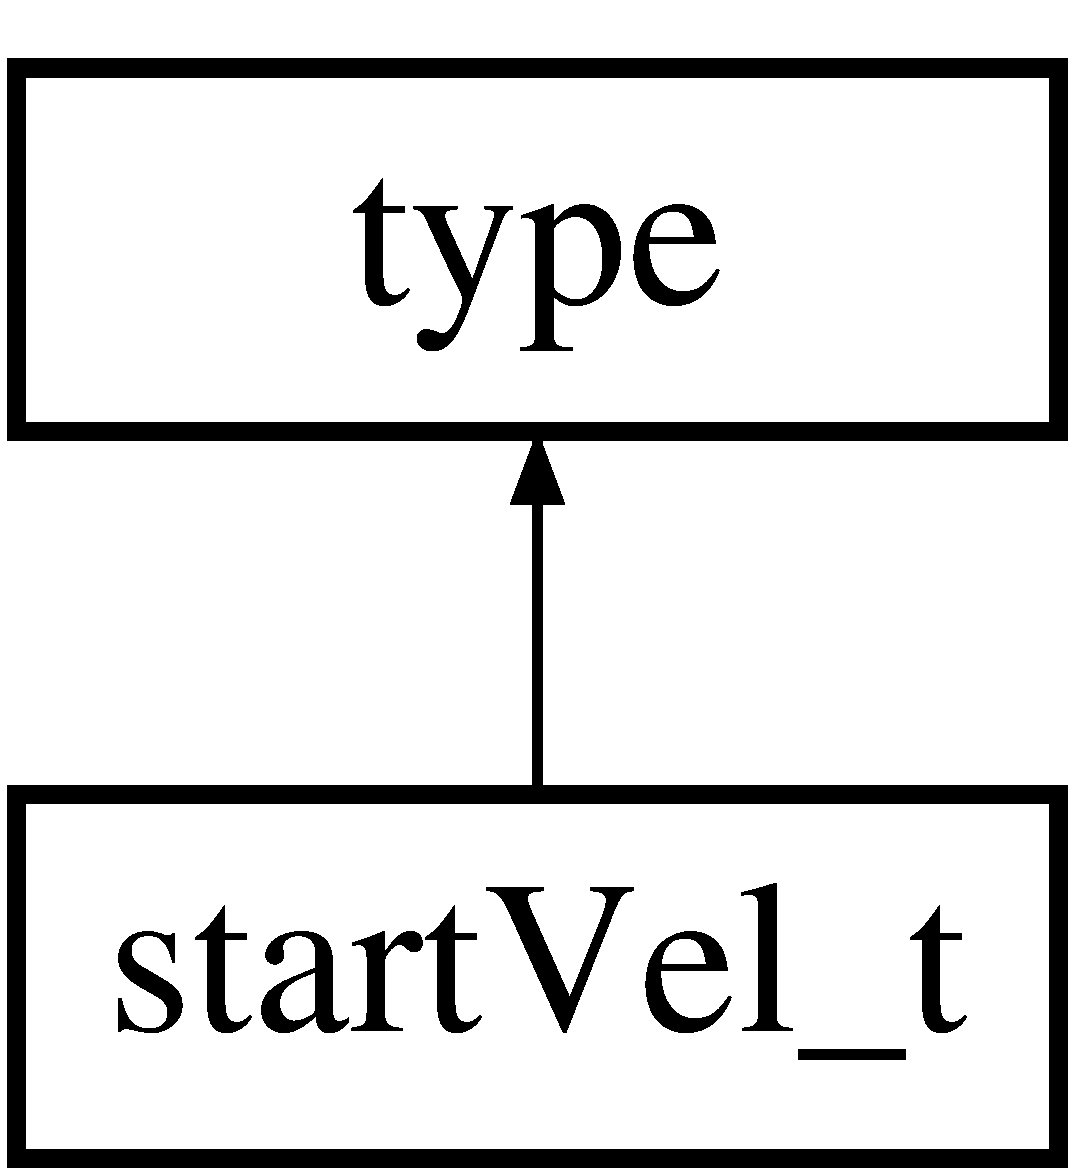
\includegraphics[height=2.000000cm]{classstartVel__t}
\end{center}
\end{figure}
\subsection*{Public Types}
\begin{DoxyCompactItemize}
\item 
typedef \-::\hyperlink{namespacexml__schema_a69bfaf24f63a8c18ebd8e21db6b343df}{xml\-\_\-schema\-::decimal} \hyperlink{classstartVel__t_a4f5683f832e22f177e3dd87c931333fb}{v\-X\-\_\-type}
\item 
typedef \\*
\-::xsd\-::cxx\-::tree\-::traits\\*
$<$ \hyperlink{classstartVel__t_a4f5683f832e22f177e3dd87c931333fb}{v\-X\-\_\-type}, char,\-::xsd\-::cxx\-::tree\-::schema\-\_\-type\-::decimal $>$ \hyperlink{classstartVel__t_aed77c2d2723441913480ac21aa2424a2}{v\-X\-\_\-traits}
\item 
typedef \-::\hyperlink{namespacexml__schema_a69bfaf24f63a8c18ebd8e21db6b343df}{xml\-\_\-schema\-::decimal} \hyperlink{classstartVel__t_ae5903806f237d8ceddf10c273a3d2002}{v\-Y\-\_\-type}
\item 
typedef \\*
\-::xsd\-::cxx\-::tree\-::traits\\*
$<$ \hyperlink{classstartVel__t_ae5903806f237d8ceddf10c273a3d2002}{v\-Y\-\_\-type}, char,\-::xsd\-::cxx\-::tree\-::schema\-\_\-type\-::decimal $>$ \hyperlink{classstartVel__t_a3048aec0781a452ce20e59c13368a62a}{v\-Y\-\_\-traits}
\item 
typedef \-::\hyperlink{namespacexml__schema_a69bfaf24f63a8c18ebd8e21db6b343df}{xml\-\_\-schema\-::decimal} \hyperlink{classstartVel__t_ae5f77efcbc29e3290d1f36cb89fbd2bf}{v\-Z\-\_\-type}
\item 
typedef \\*
\-::xsd\-::cxx\-::tree\-::traits\\*
$<$ \hyperlink{classstartVel__t_ae5f77efcbc29e3290d1f36cb89fbd2bf}{v\-Z\-\_\-type}, char,\-::xsd\-::cxx\-::tree\-::schema\-\_\-type\-::decimal $>$ \hyperlink{classstartVel__t_ad5aed7020c09d4d3eea549d4f2b34aa4}{v\-Z\-\_\-traits}
\end{DoxyCompactItemize}
\subsection*{Public Member Functions}
\begin{DoxyCompactItemize}
\item 
const \hyperlink{classstartVel__t_a4f5683f832e22f177e3dd87c931333fb}{v\-X\-\_\-type} \& \hyperlink{classstartVel__t_a2e0e855a19bf778c9cde1229bef37b3a}{v\-X} () const 
\item 
\hyperlink{classstartVel__t_a4f5683f832e22f177e3dd87c931333fb}{v\-X\-\_\-type} \& \hyperlink{classstartVel__t_ad3d45c87d3610012e06f2deead93bbbf}{v\-X} ()
\item 
void \hyperlink{classstartVel__t_a4ff02721e075f93b8fc7e0455e4a6519}{v\-X} (const \hyperlink{classstartVel__t_a4f5683f832e22f177e3dd87c931333fb}{v\-X\-\_\-type} \&x)
\item 
const \hyperlink{classstartVel__t_ae5903806f237d8ceddf10c273a3d2002}{v\-Y\-\_\-type} \& \hyperlink{classstartVel__t_a02b1baab247973fb9135d719ade4d950}{v\-Y} () const 
\item 
\hyperlink{classstartVel__t_ae5903806f237d8ceddf10c273a3d2002}{v\-Y\-\_\-type} \& \hyperlink{classstartVel__t_aa479e73253b8ae96811796d9e8dc8435}{v\-Y} ()
\item 
void \hyperlink{classstartVel__t_af3e8d9b362c5f786a4262f890ec4bce5}{v\-Y} (const \hyperlink{classstartVel__t_ae5903806f237d8ceddf10c273a3d2002}{v\-Y\-\_\-type} \&x)
\item 
const \hyperlink{classstartVel__t_ae5f77efcbc29e3290d1f36cb89fbd2bf}{v\-Z\-\_\-type} \& \hyperlink{classstartVel__t_a6d4c46e125ae7cc854b115364bddac15}{v\-Z} () const 
\item 
\hyperlink{classstartVel__t_ae5f77efcbc29e3290d1f36cb89fbd2bf}{v\-Z\-\_\-type} \& \hyperlink{classstartVel__t_a1e0414794377e90b7ac9bdebb809ca27}{v\-Z} ()
\item 
void \hyperlink{classstartVel__t_afaf5b530eef1640b63dc0e898bc3b0bc}{v\-Z} (const \hyperlink{classstartVel__t_ae5f77efcbc29e3290d1f36cb89fbd2bf}{v\-Z\-\_\-type} \&x)
\item 
\hyperlink{classstartVel__t_a174d2b2af5d886bb1cb0bca8ef8e53b2}{start\-Vel\-\_\-t} (const \hyperlink{classstartVel__t_a4f5683f832e22f177e3dd87c931333fb}{v\-X\-\_\-type} \&, const \hyperlink{classstartVel__t_ae5903806f237d8ceddf10c273a3d2002}{v\-Y\-\_\-type} \&, const \hyperlink{classstartVel__t_ae5f77efcbc29e3290d1f36cb89fbd2bf}{v\-Z\-\_\-type} \&)
\item 
\hyperlink{classstartVel__t_a83c09349ea73c7980b5dedddf8a68939}{start\-Vel\-\_\-t} (const \-::xercesc\-::\-D\-O\-M\-Element \&e,\-::\hyperlink{namespacexml__schema_a0612287d030cb2732d31a45b258fdc87}{xml\-\_\-schema\-::flags} f=0,\-::\hyperlink{namespacexml__schema_ada9aa30dc722e93ee2ed7243085402a5}{xml\-\_\-schema\-::container} $\ast$c=0)
\item 
\hyperlink{classstartVel__t_a0d6c57b67fc8159015fa7807f8f81d05}{start\-Vel\-\_\-t} (const \hyperlink{classstartVel__t}{start\-Vel\-\_\-t} \&x,\-::\hyperlink{namespacexml__schema_a0612287d030cb2732d31a45b258fdc87}{xml\-\_\-schema\-::flags} f=0,\-::\hyperlink{namespacexml__schema_ada9aa30dc722e93ee2ed7243085402a5}{xml\-\_\-schema\-::container} $\ast$c=0)
\item 
virtual \hyperlink{classstartVel__t}{start\-Vel\-\_\-t} $\ast$ \hyperlink{classstartVel__t_ac255e96e5edf2031c595e5e208d1f60d}{\-\_\-clone} (\-::\hyperlink{namespacexml__schema_a0612287d030cb2732d31a45b258fdc87}{xml\-\_\-schema\-::flags} f=0,\-::\hyperlink{namespacexml__schema_ada9aa30dc722e93ee2ed7243085402a5}{xml\-\_\-schema\-::container} $\ast$c=0) const 
\item 
virtual \hyperlink{classstartVel__t_a64d655e21bba1e5ce53ab87c0b4581c2}{$\sim$start\-Vel\-\_\-t} ()
\end{DoxyCompactItemize}
\subsection*{Protected Member Functions}
\begin{DoxyCompactItemize}
\item 
void \hyperlink{classstartVel__t_acd4c59a04a5c3ed1400ade7d2c7dc183}{parse} (\-::xsd\-::cxx\-::xml\-::dom\-::parser$<$ char $>$ \&,\-::\hyperlink{namespacexml__schema_a0612287d030cb2732d31a45b258fdc87}{xml\-\_\-schema\-::flags})
\end{DoxyCompactItemize}
\subsection*{Protected Attributes}
\begin{DoxyCompactItemize}
\item 
\-::xsd\-::cxx\-::tree\-::one$<$ \hyperlink{classstartVel__t_a4f5683f832e22f177e3dd87c931333fb}{v\-X\-\_\-type} $>$ \hyperlink{classstartVel__t_a184cae449a805c4d4d1cdbe907244de0}{v\-X\-\_\-}
\item 
\-::xsd\-::cxx\-::tree\-::one$<$ \hyperlink{classstartVel__t_ae5903806f237d8ceddf10c273a3d2002}{v\-Y\-\_\-type} $>$ \hyperlink{classstartVel__t_a4b0c39ac8d86dad52aa24ef43b44f3fb}{v\-Y\-\_\-}
\item 
\-::xsd\-::cxx\-::tree\-::one$<$ \hyperlink{classstartVel__t_ae5f77efcbc29e3290d1f36cb89fbd2bf}{v\-Z\-\_\-type} $>$ \hyperlink{classstartVel__t_a7e455032e785c56310e4f18acb650e94}{v\-Z\-\_\-}
\end{DoxyCompactItemize}


\subsection{Member Typedef Documentation}
\hypertarget{classstartVel__t_aed77c2d2723441913480ac21aa2424a2}{\index{start\-Vel\-\_\-t@{start\-Vel\-\_\-t}!v\-X\-\_\-traits@{v\-X\-\_\-traits}}
\index{v\-X\-\_\-traits@{v\-X\-\_\-traits}!startVel_t@{start\-Vel\-\_\-t}}
\subsubsection[{v\-X\-\_\-traits}]{\setlength{\rightskip}{0pt plus 5cm}typedef \-::xsd\-::cxx\-::tree\-::traits$<$ {\bf v\-X\-\_\-type}, char, \-::xsd\-::cxx\-::tree\-::schema\-\_\-type\-::decimal $>$ {\bf start\-Vel\-\_\-t\-::v\-X\-\_\-traits}}}\label{classstartVel__t_aed77c2d2723441913480ac21aa2424a2}
\hypertarget{classstartVel__t_a4f5683f832e22f177e3dd87c931333fb}{\index{start\-Vel\-\_\-t@{start\-Vel\-\_\-t}!v\-X\-\_\-type@{v\-X\-\_\-type}}
\index{v\-X\-\_\-type@{v\-X\-\_\-type}!startVel_t@{start\-Vel\-\_\-t}}
\subsubsection[{v\-X\-\_\-type}]{\setlength{\rightskip}{0pt plus 5cm}typedef \-::{\bf xml\-\_\-schema\-::decimal} {\bf start\-Vel\-\_\-t\-::v\-X\-\_\-type}}}\label{classstartVel__t_a4f5683f832e22f177e3dd87c931333fb}
\hypertarget{classstartVel__t_a3048aec0781a452ce20e59c13368a62a}{\index{start\-Vel\-\_\-t@{start\-Vel\-\_\-t}!v\-Y\-\_\-traits@{v\-Y\-\_\-traits}}
\index{v\-Y\-\_\-traits@{v\-Y\-\_\-traits}!startVel_t@{start\-Vel\-\_\-t}}
\subsubsection[{v\-Y\-\_\-traits}]{\setlength{\rightskip}{0pt plus 5cm}typedef \-::xsd\-::cxx\-::tree\-::traits$<$ {\bf v\-Y\-\_\-type}, char, \-::xsd\-::cxx\-::tree\-::schema\-\_\-type\-::decimal $>$ {\bf start\-Vel\-\_\-t\-::v\-Y\-\_\-traits}}}\label{classstartVel__t_a3048aec0781a452ce20e59c13368a62a}
\hypertarget{classstartVel__t_ae5903806f237d8ceddf10c273a3d2002}{\index{start\-Vel\-\_\-t@{start\-Vel\-\_\-t}!v\-Y\-\_\-type@{v\-Y\-\_\-type}}
\index{v\-Y\-\_\-type@{v\-Y\-\_\-type}!startVel_t@{start\-Vel\-\_\-t}}
\subsubsection[{v\-Y\-\_\-type}]{\setlength{\rightskip}{0pt plus 5cm}typedef \-::{\bf xml\-\_\-schema\-::decimal} {\bf start\-Vel\-\_\-t\-::v\-Y\-\_\-type}}}\label{classstartVel__t_ae5903806f237d8ceddf10c273a3d2002}
\hypertarget{classstartVel__t_ad5aed7020c09d4d3eea549d4f2b34aa4}{\index{start\-Vel\-\_\-t@{start\-Vel\-\_\-t}!v\-Z\-\_\-traits@{v\-Z\-\_\-traits}}
\index{v\-Z\-\_\-traits@{v\-Z\-\_\-traits}!startVel_t@{start\-Vel\-\_\-t}}
\subsubsection[{v\-Z\-\_\-traits}]{\setlength{\rightskip}{0pt plus 5cm}typedef \-::xsd\-::cxx\-::tree\-::traits$<$ {\bf v\-Z\-\_\-type}, char, \-::xsd\-::cxx\-::tree\-::schema\-\_\-type\-::decimal $>$ {\bf start\-Vel\-\_\-t\-::v\-Z\-\_\-traits}}}\label{classstartVel__t_ad5aed7020c09d4d3eea549d4f2b34aa4}
\hypertarget{classstartVel__t_ae5f77efcbc29e3290d1f36cb89fbd2bf}{\index{start\-Vel\-\_\-t@{start\-Vel\-\_\-t}!v\-Z\-\_\-type@{v\-Z\-\_\-type}}
\index{v\-Z\-\_\-type@{v\-Z\-\_\-type}!startVel_t@{start\-Vel\-\_\-t}}
\subsubsection[{v\-Z\-\_\-type}]{\setlength{\rightskip}{0pt plus 5cm}typedef \-::{\bf xml\-\_\-schema\-::decimal} {\bf start\-Vel\-\_\-t\-::v\-Z\-\_\-type}}}\label{classstartVel__t_ae5f77efcbc29e3290d1f36cb89fbd2bf}


\subsection{Constructor \& Destructor Documentation}
\hypertarget{classstartVel__t_a174d2b2af5d886bb1cb0bca8ef8e53b2}{\index{start\-Vel\-\_\-t@{start\-Vel\-\_\-t}!start\-Vel\-\_\-t@{start\-Vel\-\_\-t}}
\index{start\-Vel\-\_\-t@{start\-Vel\-\_\-t}!startVel_t@{start\-Vel\-\_\-t}}
\subsubsection[{start\-Vel\-\_\-t}]{\setlength{\rightskip}{0pt plus 5cm}start\-Vel\-\_\-t\-::start\-Vel\-\_\-t (
\begin{DoxyParamCaption}
\item[{const {\bf v\-X\-\_\-type} \&}]{v\-X, }
\item[{const {\bf v\-Y\-\_\-type} \&}]{v\-Y, }
\item[{const {\bf v\-Z\-\_\-type} \&}]{v\-Z}
\end{DoxyParamCaption}
)}}\label{classstartVel__t_a174d2b2af5d886bb1cb0bca8ef8e53b2}
\hypertarget{classstartVel__t_a83c09349ea73c7980b5dedddf8a68939}{\index{start\-Vel\-\_\-t@{start\-Vel\-\_\-t}!start\-Vel\-\_\-t@{start\-Vel\-\_\-t}}
\index{start\-Vel\-\_\-t@{start\-Vel\-\_\-t}!startVel_t@{start\-Vel\-\_\-t}}
\subsubsection[{start\-Vel\-\_\-t}]{\setlength{\rightskip}{0pt plus 5cm}start\-Vel\-\_\-t\-::start\-Vel\-\_\-t (
\begin{DoxyParamCaption}
\item[{const \-::xercesc\-::\-D\-O\-M\-Element \&}]{e, }
\item[{\-::{\bf xml\-\_\-schema\-::flags}}]{f = {\ttfamily 0}, }
\item[{\-::{\bf xml\-\_\-schema\-::container} $\ast$}]{c = {\ttfamily 0}}
\end{DoxyParamCaption}
)}}\label{classstartVel__t_a83c09349ea73c7980b5dedddf8a68939}
\hypertarget{classstartVel__t_a0d6c57b67fc8159015fa7807f8f81d05}{\index{start\-Vel\-\_\-t@{start\-Vel\-\_\-t}!start\-Vel\-\_\-t@{start\-Vel\-\_\-t}}
\index{start\-Vel\-\_\-t@{start\-Vel\-\_\-t}!startVel_t@{start\-Vel\-\_\-t}}
\subsubsection[{start\-Vel\-\_\-t}]{\setlength{\rightskip}{0pt plus 5cm}start\-Vel\-\_\-t\-::start\-Vel\-\_\-t (
\begin{DoxyParamCaption}
\item[{const {\bf start\-Vel\-\_\-t} \&}]{x, }
\item[{\-::{\bf xml\-\_\-schema\-::flags}}]{f = {\ttfamily 0}, }
\item[{\-::{\bf xml\-\_\-schema\-::container} $\ast$}]{c = {\ttfamily 0}}
\end{DoxyParamCaption}
)}}\label{classstartVel__t_a0d6c57b67fc8159015fa7807f8f81d05}
\hypertarget{classstartVel__t_a64d655e21bba1e5ce53ab87c0b4581c2}{\index{start\-Vel\-\_\-t@{start\-Vel\-\_\-t}!$\sim$start\-Vel\-\_\-t@{$\sim$start\-Vel\-\_\-t}}
\index{$\sim$start\-Vel\-\_\-t@{$\sim$start\-Vel\-\_\-t}!startVel_t@{start\-Vel\-\_\-t}}
\subsubsection[{$\sim$start\-Vel\-\_\-t}]{\setlength{\rightskip}{0pt plus 5cm}start\-Vel\-\_\-t\-::$\sim$start\-Vel\-\_\-t (
\begin{DoxyParamCaption}
{}
\end{DoxyParamCaption}
)\hspace{0.3cm}{\ttfamily [virtual]}}}\label{classstartVel__t_a64d655e21bba1e5ce53ab87c0b4581c2}


\subsection{Member Function Documentation}
\hypertarget{classstartVel__t_ac255e96e5edf2031c595e5e208d1f60d}{\index{start\-Vel\-\_\-t@{start\-Vel\-\_\-t}!\-\_\-clone@{\-\_\-clone}}
\index{\-\_\-clone@{\-\_\-clone}!startVel_t@{start\-Vel\-\_\-t}}
\subsubsection[{\-\_\-clone}]{\setlength{\rightskip}{0pt plus 5cm}{\bf start\-Vel\-\_\-t} $\ast$ start\-Vel\-\_\-t\-::\-\_\-clone (
\begin{DoxyParamCaption}
\item[{\-::{\bf xml\-\_\-schema\-::flags}}]{f = {\ttfamily 0}, }
\item[{\-::{\bf xml\-\_\-schema\-::container} $\ast$}]{c = {\ttfamily 0}}
\end{DoxyParamCaption}
) const\hspace{0.3cm}{\ttfamily [virtual]}}}\label{classstartVel__t_ac255e96e5edf2031c595e5e208d1f60d}
\hypertarget{classstartVel__t_acd4c59a04a5c3ed1400ade7d2c7dc183}{\index{start\-Vel\-\_\-t@{start\-Vel\-\_\-t}!parse@{parse}}
\index{parse@{parse}!startVel_t@{start\-Vel\-\_\-t}}
\subsubsection[{parse}]{\setlength{\rightskip}{0pt plus 5cm}void start\-Vel\-\_\-t\-::parse (
\begin{DoxyParamCaption}
\item[{\-::xsd\-::cxx\-::xml\-::dom\-::parser$<$ char $>$ \&}]{p, }
\item[{\-::{\bf xml\-\_\-schema\-::flags}}]{f}
\end{DoxyParamCaption}
)\hspace{0.3cm}{\ttfamily [protected]}}}\label{classstartVel__t_acd4c59a04a5c3ed1400ade7d2c7dc183}
\hypertarget{classstartVel__t_a2e0e855a19bf778c9cde1229bef37b3a}{\index{start\-Vel\-\_\-t@{start\-Vel\-\_\-t}!v\-X@{v\-X}}
\index{v\-X@{v\-X}!startVel_t@{start\-Vel\-\_\-t}}
\subsubsection[{v\-X}]{\setlength{\rightskip}{0pt plus 5cm}const {\bf start\-Vel\-\_\-t\-::v\-X\-\_\-type} \& start\-Vel\-\_\-t\-::v\-X (
\begin{DoxyParamCaption}
{}
\end{DoxyParamCaption}
) const}}\label{classstartVel__t_a2e0e855a19bf778c9cde1229bef37b3a}
\hypertarget{classstartVel__t_ad3d45c87d3610012e06f2deead93bbbf}{\index{start\-Vel\-\_\-t@{start\-Vel\-\_\-t}!v\-X@{v\-X}}
\index{v\-X@{v\-X}!startVel_t@{start\-Vel\-\_\-t}}
\subsubsection[{v\-X}]{\setlength{\rightskip}{0pt plus 5cm}{\bf start\-Vel\-\_\-t\-::v\-X\-\_\-type} \& start\-Vel\-\_\-t\-::v\-X (
\begin{DoxyParamCaption}
{}
\end{DoxyParamCaption}
)}}\label{classstartVel__t_ad3d45c87d3610012e06f2deead93bbbf}
\hypertarget{classstartVel__t_a4ff02721e075f93b8fc7e0455e4a6519}{\index{start\-Vel\-\_\-t@{start\-Vel\-\_\-t}!v\-X@{v\-X}}
\index{v\-X@{v\-X}!startVel_t@{start\-Vel\-\_\-t}}
\subsubsection[{v\-X}]{\setlength{\rightskip}{0pt plus 5cm}void start\-Vel\-\_\-t\-::v\-X (
\begin{DoxyParamCaption}
\item[{const {\bf v\-X\-\_\-type} \&}]{x}
\end{DoxyParamCaption}
)}}\label{classstartVel__t_a4ff02721e075f93b8fc7e0455e4a6519}
\hypertarget{classstartVel__t_a02b1baab247973fb9135d719ade4d950}{\index{start\-Vel\-\_\-t@{start\-Vel\-\_\-t}!v\-Y@{v\-Y}}
\index{v\-Y@{v\-Y}!startVel_t@{start\-Vel\-\_\-t}}
\subsubsection[{v\-Y}]{\setlength{\rightskip}{0pt plus 5cm}const {\bf start\-Vel\-\_\-t\-::v\-Y\-\_\-type} \& start\-Vel\-\_\-t\-::v\-Y (
\begin{DoxyParamCaption}
{}
\end{DoxyParamCaption}
) const}}\label{classstartVel__t_a02b1baab247973fb9135d719ade4d950}
\hypertarget{classstartVel__t_aa479e73253b8ae96811796d9e8dc8435}{\index{start\-Vel\-\_\-t@{start\-Vel\-\_\-t}!v\-Y@{v\-Y}}
\index{v\-Y@{v\-Y}!startVel_t@{start\-Vel\-\_\-t}}
\subsubsection[{v\-Y}]{\setlength{\rightskip}{0pt plus 5cm}{\bf start\-Vel\-\_\-t\-::v\-Y\-\_\-type} \& start\-Vel\-\_\-t\-::v\-Y (
\begin{DoxyParamCaption}
{}
\end{DoxyParamCaption}
)}}\label{classstartVel__t_aa479e73253b8ae96811796d9e8dc8435}
\hypertarget{classstartVel__t_af3e8d9b362c5f786a4262f890ec4bce5}{\index{start\-Vel\-\_\-t@{start\-Vel\-\_\-t}!v\-Y@{v\-Y}}
\index{v\-Y@{v\-Y}!startVel_t@{start\-Vel\-\_\-t}}
\subsubsection[{v\-Y}]{\setlength{\rightskip}{0pt plus 5cm}void start\-Vel\-\_\-t\-::v\-Y (
\begin{DoxyParamCaption}
\item[{const {\bf v\-Y\-\_\-type} \&}]{x}
\end{DoxyParamCaption}
)}}\label{classstartVel__t_af3e8d9b362c5f786a4262f890ec4bce5}
\hypertarget{classstartVel__t_a6d4c46e125ae7cc854b115364bddac15}{\index{start\-Vel\-\_\-t@{start\-Vel\-\_\-t}!v\-Z@{v\-Z}}
\index{v\-Z@{v\-Z}!startVel_t@{start\-Vel\-\_\-t}}
\subsubsection[{v\-Z}]{\setlength{\rightskip}{0pt plus 5cm}const {\bf start\-Vel\-\_\-t\-::v\-Z\-\_\-type} \& start\-Vel\-\_\-t\-::v\-Z (
\begin{DoxyParamCaption}
{}
\end{DoxyParamCaption}
) const}}\label{classstartVel__t_a6d4c46e125ae7cc854b115364bddac15}
\hypertarget{classstartVel__t_a1e0414794377e90b7ac9bdebb809ca27}{\index{start\-Vel\-\_\-t@{start\-Vel\-\_\-t}!v\-Z@{v\-Z}}
\index{v\-Z@{v\-Z}!startVel_t@{start\-Vel\-\_\-t}}
\subsubsection[{v\-Z}]{\setlength{\rightskip}{0pt plus 5cm}{\bf start\-Vel\-\_\-t\-::v\-Z\-\_\-type} \& start\-Vel\-\_\-t\-::v\-Z (
\begin{DoxyParamCaption}
{}
\end{DoxyParamCaption}
)}}\label{classstartVel__t_a1e0414794377e90b7ac9bdebb809ca27}
\hypertarget{classstartVel__t_afaf5b530eef1640b63dc0e898bc3b0bc}{\index{start\-Vel\-\_\-t@{start\-Vel\-\_\-t}!v\-Z@{v\-Z}}
\index{v\-Z@{v\-Z}!startVel_t@{start\-Vel\-\_\-t}}
\subsubsection[{v\-Z}]{\setlength{\rightskip}{0pt plus 5cm}void start\-Vel\-\_\-t\-::v\-Z (
\begin{DoxyParamCaption}
\item[{const {\bf v\-Z\-\_\-type} \&}]{x}
\end{DoxyParamCaption}
)}}\label{classstartVel__t_afaf5b530eef1640b63dc0e898bc3b0bc}


\subsection{Member Data Documentation}
\hypertarget{classstartVel__t_a184cae449a805c4d4d1cdbe907244de0}{\index{start\-Vel\-\_\-t@{start\-Vel\-\_\-t}!v\-X\-\_\-@{v\-X\-\_\-}}
\index{v\-X\-\_\-@{v\-X\-\_\-}!startVel_t@{start\-Vel\-\_\-t}}
\subsubsection[{v\-X\-\_\-}]{\setlength{\rightskip}{0pt plus 5cm}\-::xsd\-::cxx\-::tree\-::one$<$ {\bf v\-X\-\_\-type} $>$ start\-Vel\-\_\-t\-::v\-X\-\_\-\hspace{0.3cm}{\ttfamily [protected]}}}\label{classstartVel__t_a184cae449a805c4d4d1cdbe907244de0}
\hypertarget{classstartVel__t_a4b0c39ac8d86dad52aa24ef43b44f3fb}{\index{start\-Vel\-\_\-t@{start\-Vel\-\_\-t}!v\-Y\-\_\-@{v\-Y\-\_\-}}
\index{v\-Y\-\_\-@{v\-Y\-\_\-}!startVel_t@{start\-Vel\-\_\-t}}
\subsubsection[{v\-Y\-\_\-}]{\setlength{\rightskip}{0pt plus 5cm}\-::xsd\-::cxx\-::tree\-::one$<$ {\bf v\-Y\-\_\-type} $>$ start\-Vel\-\_\-t\-::v\-Y\-\_\-\hspace{0.3cm}{\ttfamily [protected]}}}\label{classstartVel__t_a4b0c39ac8d86dad52aa24ef43b44f3fb}
\hypertarget{classstartVel__t_a7e455032e785c56310e4f18acb650e94}{\index{start\-Vel\-\_\-t@{start\-Vel\-\_\-t}!v\-Z\-\_\-@{v\-Z\-\_\-}}
\index{v\-Z\-\_\-@{v\-Z\-\_\-}!startVel_t@{start\-Vel\-\_\-t}}
\subsubsection[{v\-Z\-\_\-}]{\setlength{\rightskip}{0pt plus 5cm}\-::xsd\-::cxx\-::tree\-::one$<$ {\bf v\-Z\-\_\-type} $>$ start\-Vel\-\_\-t\-::v\-Z\-\_\-\hspace{0.3cm}{\ttfamily [protected]}}}\label{classstartVel__t_a7e455032e785c56310e4f18acb650e94}


The documentation for this class was generated from the following files\-:\begin{DoxyCompactItemize}
\item 
src/utils/\hyperlink{InputSpheres_8h}{Input\-Spheres.\-h}\item 
src/utils/\hyperlink{InputSpheres_8cpp}{Input\-Spheres.\-cpp}\end{DoxyCompactItemize}

\hypertarget{classthermo__t}{\section{thermo\-\_\-t Class Reference}
\label{classthermo__t}\index{thermo\-\_\-t@{thermo\-\_\-t}}
}


{\ttfamily \#include $<$Input\-Setting.\-h$>$}

Inheritance diagram for thermo\-\_\-t\-:\begin{figure}[H]
\begin{center}
\leavevmode
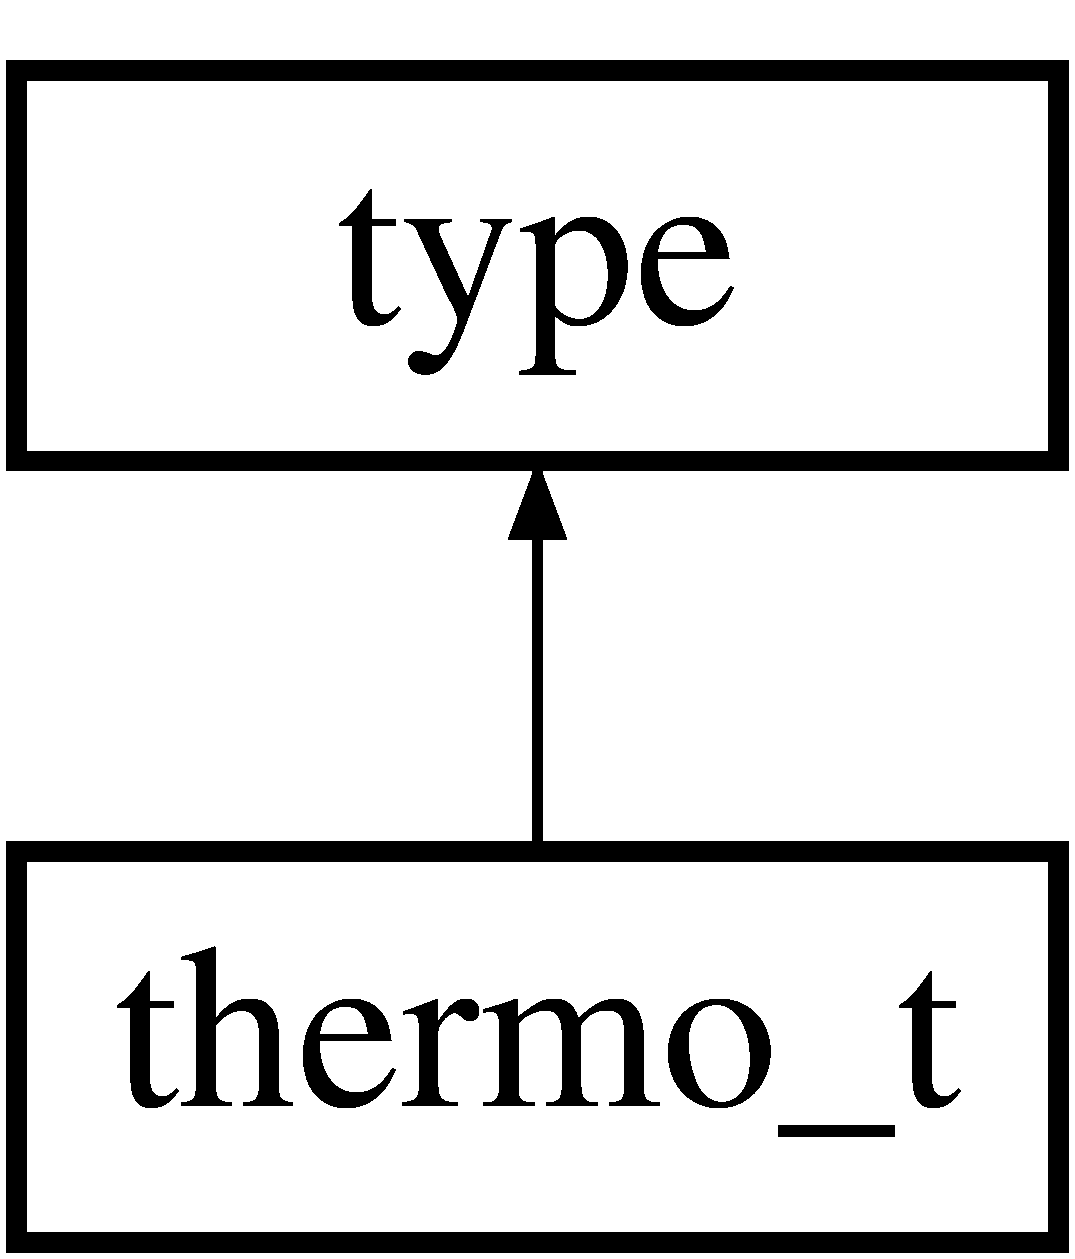
\includegraphics[height=2.000000cm]{classthermo__t}
\end{center}
\end{figure}
\subsection*{Public Types}
\begin{DoxyCompactItemize}
\item 
typedef \-::\hyperlink{namespacexml__schema_ae5ada4ec9c54b51765c3e4c0e9631bba}{xml\-\_\-schema\-::boolean} \hyperlink{classthermo__t_adf9ac04cf37c2de46153e42511aa24c2}{enabled\-\_\-type}
\item 
typedef \\*
\-::xsd\-::cxx\-::tree\-::traits\\*
$<$ \hyperlink{classthermo__t_adf9ac04cf37c2de46153e42511aa24c2}{enabled\-\_\-type}, char $>$ \hyperlink{classthermo__t_a3519860d0f767ed502e2be7b8fe6ed82}{enabled\-\_\-traits}
\item 
typedef \-::\hyperlink{namespacexml__schema_ae5ada4ec9c54b51765c3e4c0e9631bba}{xml\-\_\-schema\-::boolean} \hyperlink{classthermo__t_a124b0a16394a6c7839596d1a8ba5c35b}{brownian\-Flag\-\_\-type}
\item 
typedef \\*
\-::xsd\-::cxx\-::tree\-::traits\\*
$<$ \hyperlink{classthermo__t_a124b0a16394a6c7839596d1a8ba5c35b}{brownian\-Flag\-\_\-type}, char $>$ \hyperlink{classthermo__t_a8d99eb3bef87e3c08389e73aae1bf5d1}{brownian\-Flag\-\_\-traits}
\item 
typedef \-::\hyperlink{namespacexml__schema_a69bfaf24f63a8c18ebd8e21db6b343df}{xml\-\_\-schema\-::decimal} \hyperlink{classthermo__t_a29526c32fe31feb33a21833b0040dca7}{init\-T\-\_\-type}
\item 
typedef \\*
\-::xsd\-::cxx\-::tree\-::traits\\*
$<$ \hyperlink{classthermo__t_a29526c32fe31feb33a21833b0040dca7}{init\-T\-\_\-type}, char,\-::xsd\-::cxx\-::tree\-::schema\-\_\-type\-::decimal $>$ \hyperlink{classthermo__t_a078bc14d3b7eb9c04aa1457e24ab7c20}{init\-T\-\_\-traits}
\item 
typedef \-::\hyperlink{namespacexml__schema_a69bfaf24f63a8c18ebd8e21db6b343df}{xml\-\_\-schema\-::decimal} \hyperlink{classthermo__t_a87b71140ee6bb1936aeed1d3b79a3596}{target\-T\-\_\-type}
\item 
typedef \\*
\-::xsd\-::cxx\-::tree\-::traits\\*
$<$ \hyperlink{classthermo__t_a87b71140ee6bb1936aeed1d3b79a3596}{target\-T\-\_\-type}, char,\-::xsd\-::cxx\-::tree\-::schema\-\_\-type\-::decimal $>$ \hyperlink{classthermo__t_acf5862bbbc6795105277c01ea3797d48}{target\-T\-\_\-traits}
\item 
typedef \-::\hyperlink{namespacexml__schema_a69bfaf24f63a8c18ebd8e21db6b343df}{xml\-\_\-schema\-::decimal} \hyperlink{classthermo__t_af616f20681b799198b8c97c235092181}{delta\-T\-\_\-type}
\item 
typedef \\*
\-::xsd\-::cxx\-::tree\-::traits\\*
$<$ \hyperlink{classthermo__t_af616f20681b799198b8c97c235092181}{delta\-T\-\_\-type}, char,\-::xsd\-::cxx\-::tree\-::schema\-\_\-type\-::decimal $>$ \hyperlink{classthermo__t_a06c22e5c3354971550c96f08602ccff6}{delta\-T\-\_\-traits}
\item 
typedef \-::\hyperlink{namespacexml__schema_acfa24ac68e1a188e7f44c36f7a158bf4}{xml\-\_\-schema\-::int\-\_\-} \hyperlink{classthermo__t_a37e4458c88caf30dc0257b65e5f2af94}{n\-Thermo\-\_\-type}
\item 
typedef \\*
\-::xsd\-::cxx\-::tree\-::traits\\*
$<$ \hyperlink{classthermo__t_a37e4458c88caf30dc0257b65e5f2af94}{n\-Thermo\-\_\-type}, char $>$ \hyperlink{classthermo__t_a7733c2995c40646e0c3db3863b4a69ce}{n\-Thermo\-\_\-traits}
\item 
typedef \-::\hyperlink{namespacexml__schema_acfa24ac68e1a188e7f44c36f7a158bf4}{xml\-\_\-schema\-::int\-\_\-} \hyperlink{classthermo__t_a814f5379ac544ebfdb16162514d961c1}{n\-Delta\-\_\-type}
\item 
typedef \\*
\-::xsd\-::cxx\-::tree\-::traits\\*
$<$ \hyperlink{classthermo__t_a814f5379ac544ebfdb16162514d961c1}{n\-Delta\-\_\-type}, char $>$ \hyperlink{classthermo__t_a3e5d5b74c529cbcb267f55385bbb1088}{n\-Delta\-\_\-traits}
\end{DoxyCompactItemize}
\subsection*{Public Member Functions}
\begin{DoxyCompactItemize}
\item 
const \hyperlink{classthermo__t_adf9ac04cf37c2de46153e42511aa24c2}{enabled\-\_\-type} \& \hyperlink{classthermo__t_a3aa7ffbdb0417688a62e179a18ba7462}{enabled} () const 
\item 
\hyperlink{classthermo__t_adf9ac04cf37c2de46153e42511aa24c2}{enabled\-\_\-type} \& \hyperlink{classthermo__t_a0217614b0cde90034bd14ae06c4eec98}{enabled} ()
\item 
void \hyperlink{classthermo__t_a8a9c1776001e41905c35ae9350c1b90f}{enabled} (const \hyperlink{classthermo__t_adf9ac04cf37c2de46153e42511aa24c2}{enabled\-\_\-type} \&x)
\item 
const \hyperlink{classthermo__t_a124b0a16394a6c7839596d1a8ba5c35b}{brownian\-Flag\-\_\-type} \& \hyperlink{classthermo__t_a1be9e6c6379a040c6bc2ae7c2a170011}{brownian\-Flag} () const 
\item 
\hyperlink{classthermo__t_a124b0a16394a6c7839596d1a8ba5c35b}{brownian\-Flag\-\_\-type} \& \hyperlink{classthermo__t_a91fe0bc3623154b201d48581c8730a69}{brownian\-Flag} ()
\item 
void \hyperlink{classthermo__t_a08216f2aba58f22fbe616df2f5995ed2}{brownian\-Flag} (const \hyperlink{classthermo__t_a124b0a16394a6c7839596d1a8ba5c35b}{brownian\-Flag\-\_\-type} \&x)
\item 
const \hyperlink{classthermo__t_a29526c32fe31feb33a21833b0040dca7}{init\-T\-\_\-type} \& \hyperlink{classthermo__t_aa9c842008670ae7deb59f3a4505b282c}{init\-T} () const 
\item 
\hyperlink{classthermo__t_a29526c32fe31feb33a21833b0040dca7}{init\-T\-\_\-type} \& \hyperlink{classthermo__t_afab20b99396b34f9c656056df0d78060}{init\-T} ()
\item 
void \hyperlink{classthermo__t_a52188026af78562b9315167142ab22be}{init\-T} (const \hyperlink{classthermo__t_a29526c32fe31feb33a21833b0040dca7}{init\-T\-\_\-type} \&x)
\item 
const \hyperlink{classthermo__t_a87b71140ee6bb1936aeed1d3b79a3596}{target\-T\-\_\-type} \& \hyperlink{classthermo__t_aef84f88d4cac4cb650154f71dad6c415}{target\-T} () const 
\item 
\hyperlink{classthermo__t_a87b71140ee6bb1936aeed1d3b79a3596}{target\-T\-\_\-type} \& \hyperlink{classthermo__t_a7779b75fd22e383b11f17b05b92d98db}{target\-T} ()
\item 
void \hyperlink{classthermo__t_a0efcf3c1dae686f8c45e26148df3542b}{target\-T} (const \hyperlink{classthermo__t_a87b71140ee6bb1936aeed1d3b79a3596}{target\-T\-\_\-type} \&x)
\item 
const \hyperlink{classthermo__t_af616f20681b799198b8c97c235092181}{delta\-T\-\_\-type} \& \hyperlink{classthermo__t_afdb86658a55613b4666ffd5a48b7ebd4}{delta\-T} () const 
\item 
\hyperlink{classthermo__t_af616f20681b799198b8c97c235092181}{delta\-T\-\_\-type} \& \hyperlink{classthermo__t_a9bf5bcc2473807e26b42e211fb9bb31f}{delta\-T} ()
\item 
void \hyperlink{classthermo__t_af6e39c4c6c0140686995bb1852d05e1e}{delta\-T} (const \hyperlink{classthermo__t_af616f20681b799198b8c97c235092181}{delta\-T\-\_\-type} \&x)
\item 
const \hyperlink{classthermo__t_a37e4458c88caf30dc0257b65e5f2af94}{n\-Thermo\-\_\-type} \& \hyperlink{classthermo__t_ab9e8247db1cadc23580c27a0a1b768c2}{n\-Thermo} () const 
\item 
\hyperlink{classthermo__t_a37e4458c88caf30dc0257b65e5f2af94}{n\-Thermo\-\_\-type} \& \hyperlink{classthermo__t_a4e214b05fec430f5e6798a42261ff21f}{n\-Thermo} ()
\item 
void \hyperlink{classthermo__t_a028c387620565a248cd325753ca1def6}{n\-Thermo} (const \hyperlink{classthermo__t_a37e4458c88caf30dc0257b65e5f2af94}{n\-Thermo\-\_\-type} \&x)
\item 
const \hyperlink{classthermo__t_a814f5379ac544ebfdb16162514d961c1}{n\-Delta\-\_\-type} \& \hyperlink{classthermo__t_a8657ca0e255a05047a1fcf8d85860dd9}{n\-Delta} () const 
\item 
\hyperlink{classthermo__t_a814f5379ac544ebfdb16162514d961c1}{n\-Delta\-\_\-type} \& \hyperlink{classthermo__t_abb32968838d31fcc0fb3bdf87bf17b88}{n\-Delta} ()
\item 
void \hyperlink{classthermo__t_a7f774d8da1d510791ec3185cb3c4b23a}{n\-Delta} (const \hyperlink{classthermo__t_a814f5379ac544ebfdb16162514d961c1}{n\-Delta\-\_\-type} \&x)
\item 
\hyperlink{classthermo__t_a106c63228f15bef73116c97afc68e3e9}{thermo\-\_\-t} (const \hyperlink{classthermo__t_adf9ac04cf37c2de46153e42511aa24c2}{enabled\-\_\-type} \&, const \hyperlink{classthermo__t_a124b0a16394a6c7839596d1a8ba5c35b}{brownian\-Flag\-\_\-type} \&, const \hyperlink{classthermo__t_a29526c32fe31feb33a21833b0040dca7}{init\-T\-\_\-type} \&, const \hyperlink{classthermo__t_a87b71140ee6bb1936aeed1d3b79a3596}{target\-T\-\_\-type} \&, const \hyperlink{classthermo__t_af616f20681b799198b8c97c235092181}{delta\-T\-\_\-type} \&, const \hyperlink{classthermo__t_a37e4458c88caf30dc0257b65e5f2af94}{n\-Thermo\-\_\-type} \&, const \hyperlink{classthermo__t_a814f5379ac544ebfdb16162514d961c1}{n\-Delta\-\_\-type} \&)
\item 
\hyperlink{classthermo__t_a9d2453469c50d26154ad9126e93da768}{thermo\-\_\-t} (const \-::xercesc\-::\-D\-O\-M\-Element \&e,\-::\hyperlink{namespacexml__schema_a0612287d030cb2732d31a45b258fdc87}{xml\-\_\-schema\-::flags} f=0,\-::\hyperlink{namespacexml__schema_ada9aa30dc722e93ee2ed7243085402a5}{xml\-\_\-schema\-::container} $\ast$c=0)
\item 
\hyperlink{classthermo__t_a524ba6dfc3781a5ee2a86e674097ff00}{thermo\-\_\-t} (const \hyperlink{classthermo__t}{thermo\-\_\-t} \&x,\-::\hyperlink{namespacexml__schema_a0612287d030cb2732d31a45b258fdc87}{xml\-\_\-schema\-::flags} f=0,\-::\hyperlink{namespacexml__schema_ada9aa30dc722e93ee2ed7243085402a5}{xml\-\_\-schema\-::container} $\ast$c=0)
\item 
virtual \hyperlink{classthermo__t}{thermo\-\_\-t} $\ast$ \hyperlink{classthermo__t_a879a6032b26ce6be5227b0f9841401c2}{\-\_\-clone} (\-::\hyperlink{namespacexml__schema_a0612287d030cb2732d31a45b258fdc87}{xml\-\_\-schema\-::flags} f=0,\-::\hyperlink{namespacexml__schema_ada9aa30dc722e93ee2ed7243085402a5}{xml\-\_\-schema\-::container} $\ast$c=0) const 
\item 
virtual \hyperlink{classthermo__t_af1f580af388c6d697df6fe432928e7c3}{$\sim$thermo\-\_\-t} ()
\end{DoxyCompactItemize}
\subsection*{Protected Member Functions}
\begin{DoxyCompactItemize}
\item 
void \hyperlink{classthermo__t_ad904ca357fb42ae48a78d887fecf1f00}{parse} (\-::xsd\-::cxx\-::xml\-::dom\-::parser$<$ char $>$ \&,\-::\hyperlink{namespacexml__schema_a0612287d030cb2732d31a45b258fdc87}{xml\-\_\-schema\-::flags})
\end{DoxyCompactItemize}
\subsection*{Protected Attributes}
\begin{DoxyCompactItemize}
\item 
\-::xsd\-::cxx\-::tree\-::one\\*
$<$ \hyperlink{classthermo__t_adf9ac04cf37c2de46153e42511aa24c2}{enabled\-\_\-type} $>$ \hyperlink{classthermo__t_a943300cbe544be4d59d3962eaba464d2}{enabled\-\_\-}
\item 
\-::xsd\-::cxx\-::tree\-::one\\*
$<$ \hyperlink{classthermo__t_a124b0a16394a6c7839596d1a8ba5c35b}{brownian\-Flag\-\_\-type} $>$ \hyperlink{classthermo__t_a4e7aff42cfde2e459eae29dd08cd4335}{brownian\-Flag\-\_\-}
\item 
\-::xsd\-::cxx\-::tree\-::one$<$ \hyperlink{classthermo__t_a29526c32fe31feb33a21833b0040dca7}{init\-T\-\_\-type} $>$ \hyperlink{classthermo__t_a40762511b36c05a5923bad0cb1b49f39}{init\-T\-\_\-}
\item 
\-::xsd\-::cxx\-::tree\-::one\\*
$<$ \hyperlink{classthermo__t_a87b71140ee6bb1936aeed1d3b79a3596}{target\-T\-\_\-type} $>$ \hyperlink{classthermo__t_a1d1b8236fb2ea4426f2a83e04f8382d0}{target\-T\-\_\-}
\item 
\-::xsd\-::cxx\-::tree\-::one\\*
$<$ \hyperlink{classthermo__t_af616f20681b799198b8c97c235092181}{delta\-T\-\_\-type} $>$ \hyperlink{classthermo__t_a76fc3ddc3befeeab5226f255391a054c}{delta\-T\-\_\-}
\item 
\-::xsd\-::cxx\-::tree\-::one\\*
$<$ \hyperlink{classthermo__t_a37e4458c88caf30dc0257b65e5f2af94}{n\-Thermo\-\_\-type} $>$ \hyperlink{classthermo__t_a547f76192ba098eb94349c88427b9839}{n\-Thermo\-\_\-}
\item 
\-::xsd\-::cxx\-::tree\-::one\\*
$<$ \hyperlink{classthermo__t_a814f5379ac544ebfdb16162514d961c1}{n\-Delta\-\_\-type} $>$ \hyperlink{classthermo__t_a57e12294a2b9b189dfb9039c5d6ec8e5}{n\-Delta\-\_\-}
\end{DoxyCompactItemize}


\subsection{Member Typedef Documentation}
\hypertarget{classthermo__t_a8d99eb3bef87e3c08389e73aae1bf5d1}{\index{thermo\-\_\-t@{thermo\-\_\-t}!brownian\-Flag\-\_\-traits@{brownian\-Flag\-\_\-traits}}
\index{brownian\-Flag\-\_\-traits@{brownian\-Flag\-\_\-traits}!thermo_t@{thermo\-\_\-t}}
\subsubsection[{brownian\-Flag\-\_\-traits}]{\setlength{\rightskip}{0pt plus 5cm}typedef \-::xsd\-::cxx\-::tree\-::traits$<$ {\bf brownian\-Flag\-\_\-type}, char $>$ {\bf thermo\-\_\-t\-::brownian\-Flag\-\_\-traits}}}\label{classthermo__t_a8d99eb3bef87e3c08389e73aae1bf5d1}
\hypertarget{classthermo__t_a124b0a16394a6c7839596d1a8ba5c35b}{\index{thermo\-\_\-t@{thermo\-\_\-t}!brownian\-Flag\-\_\-type@{brownian\-Flag\-\_\-type}}
\index{brownian\-Flag\-\_\-type@{brownian\-Flag\-\_\-type}!thermo_t@{thermo\-\_\-t}}
\subsubsection[{brownian\-Flag\-\_\-type}]{\setlength{\rightskip}{0pt plus 5cm}typedef \-::{\bf xml\-\_\-schema\-::boolean} {\bf thermo\-\_\-t\-::brownian\-Flag\-\_\-type}}}\label{classthermo__t_a124b0a16394a6c7839596d1a8ba5c35b}
\hypertarget{classthermo__t_a06c22e5c3354971550c96f08602ccff6}{\index{thermo\-\_\-t@{thermo\-\_\-t}!delta\-T\-\_\-traits@{delta\-T\-\_\-traits}}
\index{delta\-T\-\_\-traits@{delta\-T\-\_\-traits}!thermo_t@{thermo\-\_\-t}}
\subsubsection[{delta\-T\-\_\-traits}]{\setlength{\rightskip}{0pt plus 5cm}typedef \-::xsd\-::cxx\-::tree\-::traits$<$ {\bf delta\-T\-\_\-type}, char, \-::xsd\-::cxx\-::tree\-::schema\-\_\-type\-::decimal $>$ {\bf thermo\-\_\-t\-::delta\-T\-\_\-traits}}}\label{classthermo__t_a06c22e5c3354971550c96f08602ccff6}
\hypertarget{classthermo__t_af616f20681b799198b8c97c235092181}{\index{thermo\-\_\-t@{thermo\-\_\-t}!delta\-T\-\_\-type@{delta\-T\-\_\-type}}
\index{delta\-T\-\_\-type@{delta\-T\-\_\-type}!thermo_t@{thermo\-\_\-t}}
\subsubsection[{delta\-T\-\_\-type}]{\setlength{\rightskip}{0pt plus 5cm}typedef \-::{\bf xml\-\_\-schema\-::decimal} {\bf thermo\-\_\-t\-::delta\-T\-\_\-type}}}\label{classthermo__t_af616f20681b799198b8c97c235092181}
\hypertarget{classthermo__t_a3519860d0f767ed502e2be7b8fe6ed82}{\index{thermo\-\_\-t@{thermo\-\_\-t}!enabled\-\_\-traits@{enabled\-\_\-traits}}
\index{enabled\-\_\-traits@{enabled\-\_\-traits}!thermo_t@{thermo\-\_\-t}}
\subsubsection[{enabled\-\_\-traits}]{\setlength{\rightskip}{0pt plus 5cm}typedef \-::xsd\-::cxx\-::tree\-::traits$<$ {\bf enabled\-\_\-type}, char $>$ {\bf thermo\-\_\-t\-::enabled\-\_\-traits}}}\label{classthermo__t_a3519860d0f767ed502e2be7b8fe6ed82}
\hypertarget{classthermo__t_adf9ac04cf37c2de46153e42511aa24c2}{\index{thermo\-\_\-t@{thermo\-\_\-t}!enabled\-\_\-type@{enabled\-\_\-type}}
\index{enabled\-\_\-type@{enabled\-\_\-type}!thermo_t@{thermo\-\_\-t}}
\subsubsection[{enabled\-\_\-type}]{\setlength{\rightskip}{0pt plus 5cm}typedef \-::{\bf xml\-\_\-schema\-::boolean} {\bf thermo\-\_\-t\-::enabled\-\_\-type}}}\label{classthermo__t_adf9ac04cf37c2de46153e42511aa24c2}
\hypertarget{classthermo__t_a078bc14d3b7eb9c04aa1457e24ab7c20}{\index{thermo\-\_\-t@{thermo\-\_\-t}!init\-T\-\_\-traits@{init\-T\-\_\-traits}}
\index{init\-T\-\_\-traits@{init\-T\-\_\-traits}!thermo_t@{thermo\-\_\-t}}
\subsubsection[{init\-T\-\_\-traits}]{\setlength{\rightskip}{0pt plus 5cm}typedef \-::xsd\-::cxx\-::tree\-::traits$<$ {\bf init\-T\-\_\-type}, char, \-::xsd\-::cxx\-::tree\-::schema\-\_\-type\-::decimal $>$ {\bf thermo\-\_\-t\-::init\-T\-\_\-traits}}}\label{classthermo__t_a078bc14d3b7eb9c04aa1457e24ab7c20}
\hypertarget{classthermo__t_a29526c32fe31feb33a21833b0040dca7}{\index{thermo\-\_\-t@{thermo\-\_\-t}!init\-T\-\_\-type@{init\-T\-\_\-type}}
\index{init\-T\-\_\-type@{init\-T\-\_\-type}!thermo_t@{thermo\-\_\-t}}
\subsubsection[{init\-T\-\_\-type}]{\setlength{\rightskip}{0pt plus 5cm}typedef \-::{\bf xml\-\_\-schema\-::decimal} {\bf thermo\-\_\-t\-::init\-T\-\_\-type}}}\label{classthermo__t_a29526c32fe31feb33a21833b0040dca7}
\hypertarget{classthermo__t_a3e5d5b74c529cbcb267f55385bbb1088}{\index{thermo\-\_\-t@{thermo\-\_\-t}!n\-Delta\-\_\-traits@{n\-Delta\-\_\-traits}}
\index{n\-Delta\-\_\-traits@{n\-Delta\-\_\-traits}!thermo_t@{thermo\-\_\-t}}
\subsubsection[{n\-Delta\-\_\-traits}]{\setlength{\rightskip}{0pt plus 5cm}typedef \-::xsd\-::cxx\-::tree\-::traits$<$ {\bf n\-Delta\-\_\-type}, char $>$ {\bf thermo\-\_\-t\-::n\-Delta\-\_\-traits}}}\label{classthermo__t_a3e5d5b74c529cbcb267f55385bbb1088}
\hypertarget{classthermo__t_a814f5379ac544ebfdb16162514d961c1}{\index{thermo\-\_\-t@{thermo\-\_\-t}!n\-Delta\-\_\-type@{n\-Delta\-\_\-type}}
\index{n\-Delta\-\_\-type@{n\-Delta\-\_\-type}!thermo_t@{thermo\-\_\-t}}
\subsubsection[{n\-Delta\-\_\-type}]{\setlength{\rightskip}{0pt plus 5cm}typedef \-::{\bf xml\-\_\-schema\-::int\-\_\-} {\bf thermo\-\_\-t\-::n\-Delta\-\_\-type}}}\label{classthermo__t_a814f5379ac544ebfdb16162514d961c1}
\hypertarget{classthermo__t_a7733c2995c40646e0c3db3863b4a69ce}{\index{thermo\-\_\-t@{thermo\-\_\-t}!n\-Thermo\-\_\-traits@{n\-Thermo\-\_\-traits}}
\index{n\-Thermo\-\_\-traits@{n\-Thermo\-\_\-traits}!thermo_t@{thermo\-\_\-t}}
\subsubsection[{n\-Thermo\-\_\-traits}]{\setlength{\rightskip}{0pt plus 5cm}typedef \-::xsd\-::cxx\-::tree\-::traits$<$ {\bf n\-Thermo\-\_\-type}, char $>$ {\bf thermo\-\_\-t\-::n\-Thermo\-\_\-traits}}}\label{classthermo__t_a7733c2995c40646e0c3db3863b4a69ce}
\hypertarget{classthermo__t_a37e4458c88caf30dc0257b65e5f2af94}{\index{thermo\-\_\-t@{thermo\-\_\-t}!n\-Thermo\-\_\-type@{n\-Thermo\-\_\-type}}
\index{n\-Thermo\-\_\-type@{n\-Thermo\-\_\-type}!thermo_t@{thermo\-\_\-t}}
\subsubsection[{n\-Thermo\-\_\-type}]{\setlength{\rightskip}{0pt plus 5cm}typedef \-::{\bf xml\-\_\-schema\-::int\-\_\-} {\bf thermo\-\_\-t\-::n\-Thermo\-\_\-type}}}\label{classthermo__t_a37e4458c88caf30dc0257b65e5f2af94}
\hypertarget{classthermo__t_acf5862bbbc6795105277c01ea3797d48}{\index{thermo\-\_\-t@{thermo\-\_\-t}!target\-T\-\_\-traits@{target\-T\-\_\-traits}}
\index{target\-T\-\_\-traits@{target\-T\-\_\-traits}!thermo_t@{thermo\-\_\-t}}
\subsubsection[{target\-T\-\_\-traits}]{\setlength{\rightskip}{0pt plus 5cm}typedef \-::xsd\-::cxx\-::tree\-::traits$<$ {\bf target\-T\-\_\-type}, char, \-::xsd\-::cxx\-::tree\-::schema\-\_\-type\-::decimal $>$ {\bf thermo\-\_\-t\-::target\-T\-\_\-traits}}}\label{classthermo__t_acf5862bbbc6795105277c01ea3797d48}
\hypertarget{classthermo__t_a87b71140ee6bb1936aeed1d3b79a3596}{\index{thermo\-\_\-t@{thermo\-\_\-t}!target\-T\-\_\-type@{target\-T\-\_\-type}}
\index{target\-T\-\_\-type@{target\-T\-\_\-type}!thermo_t@{thermo\-\_\-t}}
\subsubsection[{target\-T\-\_\-type}]{\setlength{\rightskip}{0pt plus 5cm}typedef \-::{\bf xml\-\_\-schema\-::decimal} {\bf thermo\-\_\-t\-::target\-T\-\_\-type}}}\label{classthermo__t_a87b71140ee6bb1936aeed1d3b79a3596}


\subsection{Constructor \& Destructor Documentation}
\hypertarget{classthermo__t_a106c63228f15bef73116c97afc68e3e9}{\index{thermo\-\_\-t@{thermo\-\_\-t}!thermo\-\_\-t@{thermo\-\_\-t}}
\index{thermo\-\_\-t@{thermo\-\_\-t}!thermo_t@{thermo\-\_\-t}}
\subsubsection[{thermo\-\_\-t}]{\setlength{\rightskip}{0pt plus 5cm}thermo\-\_\-t\-::thermo\-\_\-t (
\begin{DoxyParamCaption}
\item[{const {\bf enabled\-\_\-type} \&}]{enabled, }
\item[{const {\bf brownian\-Flag\-\_\-type} \&}]{brownian\-Flag, }
\item[{const {\bf init\-T\-\_\-type} \&}]{init\-T, }
\item[{const {\bf target\-T\-\_\-type} \&}]{target\-T, }
\item[{const {\bf delta\-T\-\_\-type} \&}]{delta\-T, }
\item[{const {\bf n\-Thermo\-\_\-type} \&}]{n\-Thermo, }
\item[{const {\bf n\-Delta\-\_\-type} \&}]{n\-Delta}
\end{DoxyParamCaption}
)}}\label{classthermo__t_a106c63228f15bef73116c97afc68e3e9}
\hypertarget{classthermo__t_a9d2453469c50d26154ad9126e93da768}{\index{thermo\-\_\-t@{thermo\-\_\-t}!thermo\-\_\-t@{thermo\-\_\-t}}
\index{thermo\-\_\-t@{thermo\-\_\-t}!thermo_t@{thermo\-\_\-t}}
\subsubsection[{thermo\-\_\-t}]{\setlength{\rightskip}{0pt plus 5cm}thermo\-\_\-t\-::thermo\-\_\-t (
\begin{DoxyParamCaption}
\item[{const \-::xercesc\-::\-D\-O\-M\-Element \&}]{e, }
\item[{\-::{\bf xml\-\_\-schema\-::flags}}]{f = {\ttfamily 0}, }
\item[{\-::{\bf xml\-\_\-schema\-::container} $\ast$}]{c = {\ttfamily 0}}
\end{DoxyParamCaption}
)}}\label{classthermo__t_a9d2453469c50d26154ad9126e93da768}
\hypertarget{classthermo__t_a524ba6dfc3781a5ee2a86e674097ff00}{\index{thermo\-\_\-t@{thermo\-\_\-t}!thermo\-\_\-t@{thermo\-\_\-t}}
\index{thermo\-\_\-t@{thermo\-\_\-t}!thermo_t@{thermo\-\_\-t}}
\subsubsection[{thermo\-\_\-t}]{\setlength{\rightskip}{0pt plus 5cm}thermo\-\_\-t\-::thermo\-\_\-t (
\begin{DoxyParamCaption}
\item[{const {\bf thermo\-\_\-t} \&}]{x, }
\item[{\-::{\bf xml\-\_\-schema\-::flags}}]{f = {\ttfamily 0}, }
\item[{\-::{\bf xml\-\_\-schema\-::container} $\ast$}]{c = {\ttfamily 0}}
\end{DoxyParamCaption}
)}}\label{classthermo__t_a524ba6dfc3781a5ee2a86e674097ff00}
\hypertarget{classthermo__t_af1f580af388c6d697df6fe432928e7c3}{\index{thermo\-\_\-t@{thermo\-\_\-t}!$\sim$thermo\-\_\-t@{$\sim$thermo\-\_\-t}}
\index{$\sim$thermo\-\_\-t@{$\sim$thermo\-\_\-t}!thermo_t@{thermo\-\_\-t}}
\subsubsection[{$\sim$thermo\-\_\-t}]{\setlength{\rightskip}{0pt plus 5cm}thermo\-\_\-t\-::$\sim$thermo\-\_\-t (
\begin{DoxyParamCaption}
{}
\end{DoxyParamCaption}
)\hspace{0.3cm}{\ttfamily [virtual]}}}\label{classthermo__t_af1f580af388c6d697df6fe432928e7c3}


\subsection{Member Function Documentation}
\hypertarget{classthermo__t_a879a6032b26ce6be5227b0f9841401c2}{\index{thermo\-\_\-t@{thermo\-\_\-t}!\-\_\-clone@{\-\_\-clone}}
\index{\-\_\-clone@{\-\_\-clone}!thermo_t@{thermo\-\_\-t}}
\subsubsection[{\-\_\-clone}]{\setlength{\rightskip}{0pt plus 5cm}{\bf thermo\-\_\-t} $\ast$ thermo\-\_\-t\-::\-\_\-clone (
\begin{DoxyParamCaption}
\item[{\-::{\bf xml\-\_\-schema\-::flags}}]{f = {\ttfamily 0}, }
\item[{\-::{\bf xml\-\_\-schema\-::container} $\ast$}]{c = {\ttfamily 0}}
\end{DoxyParamCaption}
) const\hspace{0.3cm}{\ttfamily [virtual]}}}\label{classthermo__t_a879a6032b26ce6be5227b0f9841401c2}
\hypertarget{classthermo__t_a1be9e6c6379a040c6bc2ae7c2a170011}{\index{thermo\-\_\-t@{thermo\-\_\-t}!brownian\-Flag@{brownian\-Flag}}
\index{brownian\-Flag@{brownian\-Flag}!thermo_t@{thermo\-\_\-t}}
\subsubsection[{brownian\-Flag}]{\setlength{\rightskip}{0pt plus 5cm}const {\bf thermo\-\_\-t\-::brownian\-Flag\-\_\-type} \& thermo\-\_\-t\-::brownian\-Flag (
\begin{DoxyParamCaption}
{}
\end{DoxyParamCaption}
) const}}\label{classthermo__t_a1be9e6c6379a040c6bc2ae7c2a170011}
\hypertarget{classthermo__t_a91fe0bc3623154b201d48581c8730a69}{\index{thermo\-\_\-t@{thermo\-\_\-t}!brownian\-Flag@{brownian\-Flag}}
\index{brownian\-Flag@{brownian\-Flag}!thermo_t@{thermo\-\_\-t}}
\subsubsection[{brownian\-Flag}]{\setlength{\rightskip}{0pt plus 5cm}{\bf thermo\-\_\-t\-::brownian\-Flag\-\_\-type} \& thermo\-\_\-t\-::brownian\-Flag (
\begin{DoxyParamCaption}
{}
\end{DoxyParamCaption}
)}}\label{classthermo__t_a91fe0bc3623154b201d48581c8730a69}
\hypertarget{classthermo__t_a08216f2aba58f22fbe616df2f5995ed2}{\index{thermo\-\_\-t@{thermo\-\_\-t}!brownian\-Flag@{brownian\-Flag}}
\index{brownian\-Flag@{brownian\-Flag}!thermo_t@{thermo\-\_\-t}}
\subsubsection[{brownian\-Flag}]{\setlength{\rightskip}{0pt plus 5cm}void thermo\-\_\-t\-::brownian\-Flag (
\begin{DoxyParamCaption}
\item[{const {\bf brownian\-Flag\-\_\-type} \&}]{x}
\end{DoxyParamCaption}
)}}\label{classthermo__t_a08216f2aba58f22fbe616df2f5995ed2}
\hypertarget{classthermo__t_afdb86658a55613b4666ffd5a48b7ebd4}{\index{thermo\-\_\-t@{thermo\-\_\-t}!delta\-T@{delta\-T}}
\index{delta\-T@{delta\-T}!thermo_t@{thermo\-\_\-t}}
\subsubsection[{delta\-T}]{\setlength{\rightskip}{0pt plus 5cm}const {\bf thermo\-\_\-t\-::delta\-T\-\_\-type} \& thermo\-\_\-t\-::delta\-T (
\begin{DoxyParamCaption}
{}
\end{DoxyParamCaption}
) const}}\label{classthermo__t_afdb86658a55613b4666ffd5a48b7ebd4}
\hypertarget{classthermo__t_a9bf5bcc2473807e26b42e211fb9bb31f}{\index{thermo\-\_\-t@{thermo\-\_\-t}!delta\-T@{delta\-T}}
\index{delta\-T@{delta\-T}!thermo_t@{thermo\-\_\-t}}
\subsubsection[{delta\-T}]{\setlength{\rightskip}{0pt plus 5cm}{\bf thermo\-\_\-t\-::delta\-T\-\_\-type} \& thermo\-\_\-t\-::delta\-T (
\begin{DoxyParamCaption}
{}
\end{DoxyParamCaption}
)}}\label{classthermo__t_a9bf5bcc2473807e26b42e211fb9bb31f}
\hypertarget{classthermo__t_af6e39c4c6c0140686995bb1852d05e1e}{\index{thermo\-\_\-t@{thermo\-\_\-t}!delta\-T@{delta\-T}}
\index{delta\-T@{delta\-T}!thermo_t@{thermo\-\_\-t}}
\subsubsection[{delta\-T}]{\setlength{\rightskip}{0pt plus 5cm}void thermo\-\_\-t\-::delta\-T (
\begin{DoxyParamCaption}
\item[{const {\bf delta\-T\-\_\-type} \&}]{x}
\end{DoxyParamCaption}
)}}\label{classthermo__t_af6e39c4c6c0140686995bb1852d05e1e}
\hypertarget{classthermo__t_a3aa7ffbdb0417688a62e179a18ba7462}{\index{thermo\-\_\-t@{thermo\-\_\-t}!enabled@{enabled}}
\index{enabled@{enabled}!thermo_t@{thermo\-\_\-t}}
\subsubsection[{enabled}]{\setlength{\rightskip}{0pt plus 5cm}const {\bf thermo\-\_\-t\-::enabled\-\_\-type} \& thermo\-\_\-t\-::enabled (
\begin{DoxyParamCaption}
{}
\end{DoxyParamCaption}
) const}}\label{classthermo__t_a3aa7ffbdb0417688a62e179a18ba7462}
\hypertarget{classthermo__t_a0217614b0cde90034bd14ae06c4eec98}{\index{thermo\-\_\-t@{thermo\-\_\-t}!enabled@{enabled}}
\index{enabled@{enabled}!thermo_t@{thermo\-\_\-t}}
\subsubsection[{enabled}]{\setlength{\rightskip}{0pt plus 5cm}{\bf thermo\-\_\-t\-::enabled\-\_\-type} \& thermo\-\_\-t\-::enabled (
\begin{DoxyParamCaption}
{}
\end{DoxyParamCaption}
)}}\label{classthermo__t_a0217614b0cde90034bd14ae06c4eec98}
\hypertarget{classthermo__t_a8a9c1776001e41905c35ae9350c1b90f}{\index{thermo\-\_\-t@{thermo\-\_\-t}!enabled@{enabled}}
\index{enabled@{enabled}!thermo_t@{thermo\-\_\-t}}
\subsubsection[{enabled}]{\setlength{\rightskip}{0pt plus 5cm}void thermo\-\_\-t\-::enabled (
\begin{DoxyParamCaption}
\item[{const {\bf enabled\-\_\-type} \&}]{x}
\end{DoxyParamCaption}
)}}\label{classthermo__t_a8a9c1776001e41905c35ae9350c1b90f}
\hypertarget{classthermo__t_aa9c842008670ae7deb59f3a4505b282c}{\index{thermo\-\_\-t@{thermo\-\_\-t}!init\-T@{init\-T}}
\index{init\-T@{init\-T}!thermo_t@{thermo\-\_\-t}}
\subsubsection[{init\-T}]{\setlength{\rightskip}{0pt plus 5cm}const {\bf thermo\-\_\-t\-::init\-T\-\_\-type} \& thermo\-\_\-t\-::init\-T (
\begin{DoxyParamCaption}
{}
\end{DoxyParamCaption}
) const}}\label{classthermo__t_aa9c842008670ae7deb59f3a4505b282c}
\hypertarget{classthermo__t_afab20b99396b34f9c656056df0d78060}{\index{thermo\-\_\-t@{thermo\-\_\-t}!init\-T@{init\-T}}
\index{init\-T@{init\-T}!thermo_t@{thermo\-\_\-t}}
\subsubsection[{init\-T}]{\setlength{\rightskip}{0pt plus 5cm}{\bf thermo\-\_\-t\-::init\-T\-\_\-type} \& thermo\-\_\-t\-::init\-T (
\begin{DoxyParamCaption}
{}
\end{DoxyParamCaption}
)}}\label{classthermo__t_afab20b99396b34f9c656056df0d78060}
\hypertarget{classthermo__t_a52188026af78562b9315167142ab22be}{\index{thermo\-\_\-t@{thermo\-\_\-t}!init\-T@{init\-T}}
\index{init\-T@{init\-T}!thermo_t@{thermo\-\_\-t}}
\subsubsection[{init\-T}]{\setlength{\rightskip}{0pt plus 5cm}void thermo\-\_\-t\-::init\-T (
\begin{DoxyParamCaption}
\item[{const {\bf init\-T\-\_\-type} \&}]{x}
\end{DoxyParamCaption}
)}}\label{classthermo__t_a52188026af78562b9315167142ab22be}
\hypertarget{classthermo__t_a8657ca0e255a05047a1fcf8d85860dd9}{\index{thermo\-\_\-t@{thermo\-\_\-t}!n\-Delta@{n\-Delta}}
\index{n\-Delta@{n\-Delta}!thermo_t@{thermo\-\_\-t}}
\subsubsection[{n\-Delta}]{\setlength{\rightskip}{0pt plus 5cm}const {\bf thermo\-\_\-t\-::n\-Delta\-\_\-type} \& thermo\-\_\-t\-::n\-Delta (
\begin{DoxyParamCaption}
{}
\end{DoxyParamCaption}
) const}}\label{classthermo__t_a8657ca0e255a05047a1fcf8d85860dd9}
\hypertarget{classthermo__t_abb32968838d31fcc0fb3bdf87bf17b88}{\index{thermo\-\_\-t@{thermo\-\_\-t}!n\-Delta@{n\-Delta}}
\index{n\-Delta@{n\-Delta}!thermo_t@{thermo\-\_\-t}}
\subsubsection[{n\-Delta}]{\setlength{\rightskip}{0pt plus 5cm}{\bf thermo\-\_\-t\-::n\-Delta\-\_\-type} \& thermo\-\_\-t\-::n\-Delta (
\begin{DoxyParamCaption}
{}
\end{DoxyParamCaption}
)}}\label{classthermo__t_abb32968838d31fcc0fb3bdf87bf17b88}
\hypertarget{classthermo__t_a7f774d8da1d510791ec3185cb3c4b23a}{\index{thermo\-\_\-t@{thermo\-\_\-t}!n\-Delta@{n\-Delta}}
\index{n\-Delta@{n\-Delta}!thermo_t@{thermo\-\_\-t}}
\subsubsection[{n\-Delta}]{\setlength{\rightskip}{0pt plus 5cm}void thermo\-\_\-t\-::n\-Delta (
\begin{DoxyParamCaption}
\item[{const {\bf n\-Delta\-\_\-type} \&}]{x}
\end{DoxyParamCaption}
)}}\label{classthermo__t_a7f774d8da1d510791ec3185cb3c4b23a}
\hypertarget{classthermo__t_ab9e8247db1cadc23580c27a0a1b768c2}{\index{thermo\-\_\-t@{thermo\-\_\-t}!n\-Thermo@{n\-Thermo}}
\index{n\-Thermo@{n\-Thermo}!thermo_t@{thermo\-\_\-t}}
\subsubsection[{n\-Thermo}]{\setlength{\rightskip}{0pt plus 5cm}const {\bf thermo\-\_\-t\-::n\-Thermo\-\_\-type} \& thermo\-\_\-t\-::n\-Thermo (
\begin{DoxyParamCaption}
{}
\end{DoxyParamCaption}
) const}}\label{classthermo__t_ab9e8247db1cadc23580c27a0a1b768c2}
\hypertarget{classthermo__t_a4e214b05fec430f5e6798a42261ff21f}{\index{thermo\-\_\-t@{thermo\-\_\-t}!n\-Thermo@{n\-Thermo}}
\index{n\-Thermo@{n\-Thermo}!thermo_t@{thermo\-\_\-t}}
\subsubsection[{n\-Thermo}]{\setlength{\rightskip}{0pt plus 5cm}{\bf thermo\-\_\-t\-::n\-Thermo\-\_\-type} \& thermo\-\_\-t\-::n\-Thermo (
\begin{DoxyParamCaption}
{}
\end{DoxyParamCaption}
)}}\label{classthermo__t_a4e214b05fec430f5e6798a42261ff21f}
\hypertarget{classthermo__t_a028c387620565a248cd325753ca1def6}{\index{thermo\-\_\-t@{thermo\-\_\-t}!n\-Thermo@{n\-Thermo}}
\index{n\-Thermo@{n\-Thermo}!thermo_t@{thermo\-\_\-t}}
\subsubsection[{n\-Thermo}]{\setlength{\rightskip}{0pt plus 5cm}void thermo\-\_\-t\-::n\-Thermo (
\begin{DoxyParamCaption}
\item[{const {\bf n\-Thermo\-\_\-type} \&}]{x}
\end{DoxyParamCaption}
)}}\label{classthermo__t_a028c387620565a248cd325753ca1def6}
\hypertarget{classthermo__t_ad904ca357fb42ae48a78d887fecf1f00}{\index{thermo\-\_\-t@{thermo\-\_\-t}!parse@{parse}}
\index{parse@{parse}!thermo_t@{thermo\-\_\-t}}
\subsubsection[{parse}]{\setlength{\rightskip}{0pt plus 5cm}void thermo\-\_\-t\-::parse (
\begin{DoxyParamCaption}
\item[{\-::xsd\-::cxx\-::xml\-::dom\-::parser$<$ char $>$ \&}]{p, }
\item[{\-::{\bf xml\-\_\-schema\-::flags}}]{f}
\end{DoxyParamCaption}
)\hspace{0.3cm}{\ttfamily [protected]}}}\label{classthermo__t_ad904ca357fb42ae48a78d887fecf1f00}
\hypertarget{classthermo__t_aef84f88d4cac4cb650154f71dad6c415}{\index{thermo\-\_\-t@{thermo\-\_\-t}!target\-T@{target\-T}}
\index{target\-T@{target\-T}!thermo_t@{thermo\-\_\-t}}
\subsubsection[{target\-T}]{\setlength{\rightskip}{0pt plus 5cm}const {\bf thermo\-\_\-t\-::target\-T\-\_\-type} \& thermo\-\_\-t\-::target\-T (
\begin{DoxyParamCaption}
{}
\end{DoxyParamCaption}
) const}}\label{classthermo__t_aef84f88d4cac4cb650154f71dad6c415}
\hypertarget{classthermo__t_a7779b75fd22e383b11f17b05b92d98db}{\index{thermo\-\_\-t@{thermo\-\_\-t}!target\-T@{target\-T}}
\index{target\-T@{target\-T}!thermo_t@{thermo\-\_\-t}}
\subsubsection[{target\-T}]{\setlength{\rightskip}{0pt plus 5cm}{\bf thermo\-\_\-t\-::target\-T\-\_\-type} \& thermo\-\_\-t\-::target\-T (
\begin{DoxyParamCaption}
{}
\end{DoxyParamCaption}
)}}\label{classthermo__t_a7779b75fd22e383b11f17b05b92d98db}
\hypertarget{classthermo__t_a0efcf3c1dae686f8c45e26148df3542b}{\index{thermo\-\_\-t@{thermo\-\_\-t}!target\-T@{target\-T}}
\index{target\-T@{target\-T}!thermo_t@{thermo\-\_\-t}}
\subsubsection[{target\-T}]{\setlength{\rightskip}{0pt plus 5cm}void thermo\-\_\-t\-::target\-T (
\begin{DoxyParamCaption}
\item[{const {\bf target\-T\-\_\-type} \&}]{x}
\end{DoxyParamCaption}
)}}\label{classthermo__t_a0efcf3c1dae686f8c45e26148df3542b}


\subsection{Member Data Documentation}
\hypertarget{classthermo__t_a4e7aff42cfde2e459eae29dd08cd4335}{\index{thermo\-\_\-t@{thermo\-\_\-t}!brownian\-Flag\-\_\-@{brownian\-Flag\-\_\-}}
\index{brownian\-Flag\-\_\-@{brownian\-Flag\-\_\-}!thermo_t@{thermo\-\_\-t}}
\subsubsection[{brownian\-Flag\-\_\-}]{\setlength{\rightskip}{0pt plus 5cm}\-::xsd\-::cxx\-::tree\-::one$<$ {\bf brownian\-Flag\-\_\-type} $>$ thermo\-\_\-t\-::brownian\-Flag\-\_\-\hspace{0.3cm}{\ttfamily [protected]}}}\label{classthermo__t_a4e7aff42cfde2e459eae29dd08cd4335}
\hypertarget{classthermo__t_a76fc3ddc3befeeab5226f255391a054c}{\index{thermo\-\_\-t@{thermo\-\_\-t}!delta\-T\-\_\-@{delta\-T\-\_\-}}
\index{delta\-T\-\_\-@{delta\-T\-\_\-}!thermo_t@{thermo\-\_\-t}}
\subsubsection[{delta\-T\-\_\-}]{\setlength{\rightskip}{0pt plus 5cm}\-::xsd\-::cxx\-::tree\-::one$<$ {\bf delta\-T\-\_\-type} $>$ thermo\-\_\-t\-::delta\-T\-\_\-\hspace{0.3cm}{\ttfamily [protected]}}}\label{classthermo__t_a76fc3ddc3befeeab5226f255391a054c}
\hypertarget{classthermo__t_a943300cbe544be4d59d3962eaba464d2}{\index{thermo\-\_\-t@{thermo\-\_\-t}!enabled\-\_\-@{enabled\-\_\-}}
\index{enabled\-\_\-@{enabled\-\_\-}!thermo_t@{thermo\-\_\-t}}
\subsubsection[{enabled\-\_\-}]{\setlength{\rightskip}{0pt plus 5cm}\-::xsd\-::cxx\-::tree\-::one$<$ {\bf enabled\-\_\-type} $>$ thermo\-\_\-t\-::enabled\-\_\-\hspace{0.3cm}{\ttfamily [protected]}}}\label{classthermo__t_a943300cbe544be4d59d3962eaba464d2}
\hypertarget{classthermo__t_a40762511b36c05a5923bad0cb1b49f39}{\index{thermo\-\_\-t@{thermo\-\_\-t}!init\-T\-\_\-@{init\-T\-\_\-}}
\index{init\-T\-\_\-@{init\-T\-\_\-}!thermo_t@{thermo\-\_\-t}}
\subsubsection[{init\-T\-\_\-}]{\setlength{\rightskip}{0pt plus 5cm}\-::xsd\-::cxx\-::tree\-::one$<$ {\bf init\-T\-\_\-type} $>$ thermo\-\_\-t\-::init\-T\-\_\-\hspace{0.3cm}{\ttfamily [protected]}}}\label{classthermo__t_a40762511b36c05a5923bad0cb1b49f39}
\hypertarget{classthermo__t_a57e12294a2b9b189dfb9039c5d6ec8e5}{\index{thermo\-\_\-t@{thermo\-\_\-t}!n\-Delta\-\_\-@{n\-Delta\-\_\-}}
\index{n\-Delta\-\_\-@{n\-Delta\-\_\-}!thermo_t@{thermo\-\_\-t}}
\subsubsection[{n\-Delta\-\_\-}]{\setlength{\rightskip}{0pt plus 5cm}\-::xsd\-::cxx\-::tree\-::one$<$ {\bf n\-Delta\-\_\-type} $>$ thermo\-\_\-t\-::n\-Delta\-\_\-\hspace{0.3cm}{\ttfamily [protected]}}}\label{classthermo__t_a57e12294a2b9b189dfb9039c5d6ec8e5}
\hypertarget{classthermo__t_a547f76192ba098eb94349c88427b9839}{\index{thermo\-\_\-t@{thermo\-\_\-t}!n\-Thermo\-\_\-@{n\-Thermo\-\_\-}}
\index{n\-Thermo\-\_\-@{n\-Thermo\-\_\-}!thermo_t@{thermo\-\_\-t}}
\subsubsection[{n\-Thermo\-\_\-}]{\setlength{\rightskip}{0pt plus 5cm}\-::xsd\-::cxx\-::tree\-::one$<$ {\bf n\-Thermo\-\_\-type} $>$ thermo\-\_\-t\-::n\-Thermo\-\_\-\hspace{0.3cm}{\ttfamily [protected]}}}\label{classthermo__t_a547f76192ba098eb94349c88427b9839}
\hypertarget{classthermo__t_a1d1b8236fb2ea4426f2a83e04f8382d0}{\index{thermo\-\_\-t@{thermo\-\_\-t}!target\-T\-\_\-@{target\-T\-\_\-}}
\index{target\-T\-\_\-@{target\-T\-\_\-}!thermo_t@{thermo\-\_\-t}}
\subsubsection[{target\-T\-\_\-}]{\setlength{\rightskip}{0pt plus 5cm}\-::xsd\-::cxx\-::tree\-::one$<$ {\bf target\-T\-\_\-type} $>$ thermo\-\_\-t\-::target\-T\-\_\-\hspace{0.3cm}{\ttfamily [protected]}}}\label{classthermo__t_a1d1b8236fb2ea4426f2a83e04f8382d0}


The documentation for this class was generated from the following files\-:\begin{DoxyCompactItemize}
\item 
src/utils/\hyperlink{InputSetting_8h}{Input\-Setting.\-h}\item 
src/utils/\hyperlink{InputSetting_8cpp}{Input\-Setting.\-cpp}\end{DoxyCompactItemize}

\hypertarget{classThermostat}{\section{Thermostat Class Reference}
\label{classThermostat}\index{Thermostat@{Thermostat}}
}


{\ttfamily \#include $<$Thermostat.\-h$>$}

\subsection*{Public Member Functions}
\begin{DoxyCompactItemize}
\item 
\hyperlink{classThermostat_a67cfc54f1cff43f4cd92c58e3be01919}{Thermostat} ()
\item 
\hyperlink{classThermostat_a363b4ca8da84980f9f8765acdc07e80d}{Thermostat} (const std\-::string filename)
\item 
virtual \hyperlink{classThermostat_a287977ba29071ae8c927d68e556c3098}{$\sim$\-Thermostat} ()
\item 
\hyperlink{classThermostat_a2151c3d615d12cd4f4d54a4e4f857142}{Thermostat} (double \hyperlink{classThermostat_a663a14e3a4b7bf439c92fbcd0ebac7a3}{T\-\_\-init}, double \hyperlink{classThermostat_a63c42ca7dee6ed5237d8be9e9c3f1228}{T\-\_\-target}, double \hyperlink{classThermostat_a1628e1ae6669caacbb02da75423cc35c}{delta\-\_\-\-T}, int \hyperlink{classThermostat_a25a5e29fbae46ffb4152655b3ba062cf}{n\-\_\-thermo}, int \hyperlink{classThermostat_a9a2715e81ed11171e530e2d22a682244}{n\-\_\-delta}, bool \hyperlink{classThermostat_a86ae25ddde5ab2ecd7d70a50c8a72823}{brownian\-\_\-flag}, bool \hyperlink{classThermostat_ae383f11c6ba111f1f14b470a17655d04}{enabled})
\item 
double \hyperlink{classThermostat_aa9f9d0b9ca412ff73124a8fef0882740}{get\-E\-Kin} (std\-::list$<$ \hyperlink{classParticle}{Particle} $\ast$ $>$ \&par\-List)
\item 
double \hyperlink{classThermostat_aa0e58f2c8b189f31c949d9cd1870aa6f}{get\-Mean\-V} (std\-::list$<$ \hyperlink{classParticle}{Particle} $\ast$ $>$ \&par\-List, int dim, double \hyperlink{MolSim_8cpp_aba71f400e3a017e824e2a70435a75542}{mass})
\item 
void \hyperlink{classThermostat_a2a3f40b013805848e2092d8e2579e100}{set\-Thermo} (std\-::list$<$ \hyperlink{classParticle}{Particle} $\ast$ $>$ \&par\-List, int dim, double temperature)
\item 
double \& \hyperlink{classThermostat_a7f5f9fb551b0a5f3dd183cd4f0cec3fa}{get\-T\-\_\-init} ()
\item 
double \& \hyperlink{classThermostat_a83b2ed651c6ef97fdb306791c056e790}{get\-T\-\_\-target} ()
\item 
double \& \hyperlink{classThermostat_a4dfa1bf0c8250109f621ca67dc4b9d21}{get\-Delta\-\_\-\-T} ()
\item 
int \& \hyperlink{classThermostat_ac88fdcd49a14f5c28fd2433274c1ee94}{getn\-\_\-thermo} ()
\item 
int \& \hyperlink{classThermostat_a4874b207620e187886359077e5928df8}{getn\-\_\-delta} ()
\item 
bool \& \hyperlink{classThermostat_a959655befa411badcfff9919c0fc9417}{get\-Brownian\-\_\-flag} ()
\item 
bool \& \hyperlink{classThermostat_a5a270ca35680c0f15cee0438e7e2c096}{get\-Enabled} ()
\end{DoxyCompactItemize}
\subsection*{Private Attributes}
\begin{DoxyCompactItemize}
\item 
bool \hyperlink{classThermostat_ae383f11c6ba111f1f14b470a17655d04}{enabled}
\item 
double \hyperlink{classThermostat_a663a14e3a4b7bf439c92fbcd0ebac7a3}{T\-\_\-init}
\item 
double \hyperlink{classThermostat_a63c42ca7dee6ed5237d8be9e9c3f1228}{T\-\_\-target}
\item 
double \hyperlink{classThermostat_a1628e1ae6669caacbb02da75423cc35c}{delta\-\_\-\-T}
\item 
int \hyperlink{classThermostat_a25a5e29fbae46ffb4152655b3ba062cf}{n\-\_\-thermo}
\item 
int \hyperlink{classThermostat_a9a2715e81ed11171e530e2d22a682244}{n\-\_\-delta}
\item 
bool \hyperlink{classThermostat_a86ae25ddde5ab2ecd7d70a50c8a72823}{brownian\-\_\-flag}
\end{DoxyCompactItemize}


\subsection{Constructor \& Destructor Documentation}
\hypertarget{classThermostat_a67cfc54f1cff43f4cd92c58e3be01919}{\index{Thermostat@{Thermostat}!Thermostat@{Thermostat}}
\index{Thermostat@{Thermostat}!Thermostat@{Thermostat}}
\subsubsection[{Thermostat}]{\setlength{\rightskip}{0pt plus 5cm}Thermostat\-::\-Thermostat (
\begin{DoxyParamCaption}
{}
\end{DoxyParamCaption}
)}}\label{classThermostat_a67cfc54f1cff43f4cd92c58e3be01919}
Default constructor. \hypertarget{classThermostat_a363b4ca8da84980f9f8765acdc07e80d}{\index{Thermostat@{Thermostat}!Thermostat@{Thermostat}}
\index{Thermostat@{Thermostat}!Thermostat@{Thermostat}}
\subsubsection[{Thermostat}]{\setlength{\rightskip}{0pt plus 5cm}Thermostat\-::\-Thermostat (
\begin{DoxyParamCaption}
\item[{const std\-::string}]{filename}
\end{DoxyParamCaption}
)}}\label{classThermostat_a363b4ca8da84980f9f8765acdc07e80d}
Main constructor, which will read information from filename and extract all needed information for thermostat. \hypertarget{classThermostat_a287977ba29071ae8c927d68e556c3098}{\index{Thermostat@{Thermostat}!$\sim$\-Thermostat@{$\sim$\-Thermostat}}
\index{$\sim$\-Thermostat@{$\sim$\-Thermostat}!Thermostat@{Thermostat}}
\subsubsection[{$\sim$\-Thermostat}]{\setlength{\rightskip}{0pt plus 5cm}Thermostat\-::$\sim$\-Thermostat (
\begin{DoxyParamCaption}
{}
\end{DoxyParamCaption}
)\hspace{0.3cm}{\ttfamily [virtual]}}}\label{classThermostat_a287977ba29071ae8c927d68e556c3098}
\hypertarget{classThermostat_a2151c3d615d12cd4f4d54a4e4f857142}{\index{Thermostat@{Thermostat}!Thermostat@{Thermostat}}
\index{Thermostat@{Thermostat}!Thermostat@{Thermostat}}
\subsubsection[{Thermostat}]{\setlength{\rightskip}{0pt plus 5cm}Thermostat\-::\-Thermostat (
\begin{DoxyParamCaption}
\item[{double}]{T\-\_\-init, }
\item[{double}]{T\-\_\-target, }
\item[{double}]{delta\-\_\-\-T, }
\item[{int}]{n\-\_\-thermo, }
\item[{int}]{n\-\_\-delta, }
\item[{bool}]{brownian\-\_\-flag, }
\item[{bool}]{enabled}
\end{DoxyParamCaption}
)}}\label{classThermostat_a2151c3d615d12cd4f4d54a4e4f857142}
Secondary constructor, which will initialize a thermostat with given parameters.


\begin{DoxyParams}[1]{Parameters}
\mbox{\tt in}  & {\em T\-\_\-init} & init temperature \\
\hline
\mbox{\tt in}  & {\em T\-\_\-target} & target temperature \\
\hline
\mbox{\tt in}  & {\em delta\-\_\-\-T} & temperature difference \\
\hline
\mbox{\tt in}  & {\em n\-\_\-thermo} & timesteps, after which thermostat will be applied \\
\hline
\mbox{\tt in}  & {\em n\-\_\-delta} & timesteps, after which temperature will be updated \\
\hline
\mbox{\tt in}  & {\em brownian\-\_\-flag} & option for Brownian Motion \\
\hline
\mbox{\tt in}  & {\em enabled} & option for switching thermostat on/off \\
\hline
\end{DoxyParams}


\subsection{Member Function Documentation}
\hypertarget{classThermostat_a959655befa411badcfff9919c0fc9417}{\index{Thermostat@{Thermostat}!get\-Brownian\-\_\-flag@{get\-Brownian\-\_\-flag}}
\index{get\-Brownian\-\_\-flag@{get\-Brownian\-\_\-flag}!Thermostat@{Thermostat}}
\subsubsection[{get\-Brownian\-\_\-flag}]{\setlength{\rightskip}{0pt plus 5cm}bool \& Thermostat\-::get\-Brownian\-\_\-flag (
\begin{DoxyParamCaption}
{}
\end{DoxyParamCaption}
)}}\label{classThermostat_a959655befa411badcfff9919c0fc9417}
\begin{DoxyReturn}{Returns}
option for Brownian Motion. 
\end{DoxyReturn}
\hypertarget{classThermostat_a4dfa1bf0c8250109f621ca67dc4b9d21}{\index{Thermostat@{Thermostat}!get\-Delta\-\_\-\-T@{get\-Delta\-\_\-\-T}}
\index{get\-Delta\-\_\-\-T@{get\-Delta\-\_\-\-T}!Thermostat@{Thermostat}}
\subsubsection[{get\-Delta\-\_\-\-T}]{\setlength{\rightskip}{0pt plus 5cm}double \& Thermostat\-::get\-Delta\-\_\-\-T (
\begin{DoxyParamCaption}
{}
\end{DoxyParamCaption}
)}}\label{classThermostat_a4dfa1bf0c8250109f621ca67dc4b9d21}
\begin{DoxyReturn}{Returns}
temperature difference, which will be added every n\-\_\-delta timesteps. 
\end{DoxyReturn}
\hypertarget{classThermostat_aa9f9d0b9ca412ff73124a8fef0882740}{\index{Thermostat@{Thermostat}!get\-E\-Kin@{get\-E\-Kin}}
\index{get\-E\-Kin@{get\-E\-Kin}!Thermostat@{Thermostat}}
\subsubsection[{get\-E\-Kin}]{\setlength{\rightskip}{0pt plus 5cm}double Thermostat\-::get\-E\-Kin (
\begin{DoxyParamCaption}
\item[{std\-::list$<$ {\bf Particle} $\ast$ $>$ \&}]{par\-List}
\end{DoxyParamCaption}
)}}\label{classThermostat_aa9f9d0b9ca412ff73124a8fef0882740}
\begin{DoxyReturn}{Returns}
kinetic energy of the system.
\end{DoxyReturn}

\begin{DoxyParams}[1]{Parameters}
\mbox{\tt in}  & {\em par\-List} & a list of pointers of particles \\
\hline
\end{DoxyParams}
\hypertarget{classThermostat_a5a270ca35680c0f15cee0438e7e2c096}{\index{Thermostat@{Thermostat}!get\-Enabled@{get\-Enabled}}
\index{get\-Enabled@{get\-Enabled}!Thermostat@{Thermostat}}
\subsubsection[{get\-Enabled}]{\setlength{\rightskip}{0pt plus 5cm}bool \& Thermostat\-::get\-Enabled (
\begin{DoxyParamCaption}
{}
\end{DoxyParamCaption}
)}}\label{classThermostat_a5a270ca35680c0f15cee0438e7e2c096}
\begin{DoxyReturn}{Returns}
option for switching thermostat on/off. 
\end{DoxyReturn}
\hypertarget{classThermostat_aa0e58f2c8b189f31c949d9cd1870aa6f}{\index{Thermostat@{Thermostat}!get\-Mean\-V@{get\-Mean\-V}}
\index{get\-Mean\-V@{get\-Mean\-V}!Thermostat@{Thermostat}}
\subsubsection[{get\-Mean\-V}]{\setlength{\rightskip}{0pt plus 5cm}double Thermostat\-::get\-Mean\-V (
\begin{DoxyParamCaption}
\item[{std\-::list$<$ {\bf Particle} $\ast$ $>$ \&}]{par\-List, }
\item[{int}]{dim, }
\item[{double}]{mass}
\end{DoxyParamCaption}
)}}\label{classThermostat_aa0e58f2c8b189f31c949d9cd1870aa6f}
\begin{DoxyReturn}{Returns}
mean velocity of the system for Brownian Motion.
\end{DoxyReturn}

\begin{DoxyParams}[1]{Parameters}
\mbox{\tt in}  & {\em par\-List} & a list of pointers of particles \\
\hline
\mbox{\tt in}  & {\em dim} & number of dimensions (2 or 3) \\
\hline
\mbox{\tt in}  & {\em mass} & mass of each particle in the system \\
\hline
\end{DoxyParams}
\hypertarget{classThermostat_a4874b207620e187886359077e5928df8}{\index{Thermostat@{Thermostat}!getn\-\_\-delta@{getn\-\_\-delta}}
\index{getn\-\_\-delta@{getn\-\_\-delta}!Thermostat@{Thermostat}}
\subsubsection[{getn\-\_\-delta}]{\setlength{\rightskip}{0pt plus 5cm}int \& Thermostat\-::getn\-\_\-delta (
\begin{DoxyParamCaption}
{}
\end{DoxyParamCaption}
)}}\label{classThermostat_a4874b207620e187886359077e5928df8}
\begin{DoxyReturn}{Returns}
timesteps, after which the temperature will be updated. 
\end{DoxyReturn}
\hypertarget{classThermostat_ac88fdcd49a14f5c28fd2433274c1ee94}{\index{Thermostat@{Thermostat}!getn\-\_\-thermo@{getn\-\_\-thermo}}
\index{getn\-\_\-thermo@{getn\-\_\-thermo}!Thermostat@{Thermostat}}
\subsubsection[{getn\-\_\-thermo}]{\setlength{\rightskip}{0pt plus 5cm}int \& Thermostat\-::getn\-\_\-thermo (
\begin{DoxyParamCaption}
{}
\end{DoxyParamCaption}
)}}\label{classThermostat_ac88fdcd49a14f5c28fd2433274c1ee94}
\begin{DoxyReturn}{Returns}
timesteps, after which thermostat will be applied. 
\end{DoxyReturn}
\hypertarget{classThermostat_a7f5f9fb551b0a5f3dd183cd4f0cec3fa}{\index{Thermostat@{Thermostat}!get\-T\-\_\-init@{get\-T\-\_\-init}}
\index{get\-T\-\_\-init@{get\-T\-\_\-init}!Thermostat@{Thermostat}}
\subsubsection[{get\-T\-\_\-init}]{\setlength{\rightskip}{0pt plus 5cm}double \& Thermostat\-::get\-T\-\_\-init (
\begin{DoxyParamCaption}
{}
\end{DoxyParamCaption}
)}}\label{classThermostat_a7f5f9fb551b0a5f3dd183cd4f0cec3fa}
\begin{DoxyReturn}{Returns}
init temperature of the system. 
\end{DoxyReturn}
\hypertarget{classThermostat_a83b2ed651c6ef97fdb306791c056e790}{\index{Thermostat@{Thermostat}!get\-T\-\_\-target@{get\-T\-\_\-target}}
\index{get\-T\-\_\-target@{get\-T\-\_\-target}!Thermostat@{Thermostat}}
\subsubsection[{get\-T\-\_\-target}]{\setlength{\rightskip}{0pt plus 5cm}double \& Thermostat\-::get\-T\-\_\-target (
\begin{DoxyParamCaption}
{}
\end{DoxyParamCaption}
)}}\label{classThermostat_a83b2ed651c6ef97fdb306791c056e790}
\begin{DoxyReturn}{Returns}
target temperature of the system. 
\end{DoxyReturn}
\hypertarget{classThermostat_a2a3f40b013805848e2092d8e2579e100}{\index{Thermostat@{Thermostat}!set\-Thermo@{set\-Thermo}}
\index{set\-Thermo@{set\-Thermo}!Thermostat@{Thermostat}}
\subsubsection[{set\-Thermo}]{\setlength{\rightskip}{0pt plus 5cm}void Thermostat\-::set\-Thermo (
\begin{DoxyParamCaption}
\item[{std\-::list$<$ {\bf Particle} $\ast$ $>$ \&}]{par\-List, }
\item[{int}]{dim, }
\item[{double}]{temperature}
\end{DoxyParamCaption}
)}}\label{classThermostat_a2a3f40b013805848e2092d8e2579e100}
Setter.


\begin{DoxyParams}[1]{Parameters}
\mbox{\tt in}  & {\em par\-List} & a list of pointers of particles \\
\hline
\mbox{\tt in}  & {\em dim} & number of dimensions (2 or 3) \\
\hline
\mbox{\tt in}  & {\em temperature} & desired temperature, which will be reached after the thermostat was set. \\
\hline
\end{DoxyParams}


\subsection{Member Data Documentation}
\hypertarget{classThermostat_a86ae25ddde5ab2ecd7d70a50c8a72823}{\index{Thermostat@{Thermostat}!brownian\-\_\-flag@{brownian\-\_\-flag}}
\index{brownian\-\_\-flag@{brownian\-\_\-flag}!Thermostat@{Thermostat}}
\subsubsection[{brownian\-\_\-flag}]{\setlength{\rightskip}{0pt plus 5cm}bool Thermostat\-::brownian\-\_\-flag\hspace{0.3cm}{\ttfamily [private]}}}\label{classThermostat_a86ae25ddde5ab2ecd7d70a50c8a72823}
True if Brownian Motion is needed, false if not. \hypertarget{classThermostat_a1628e1ae6669caacbb02da75423cc35c}{\index{Thermostat@{Thermostat}!delta\-\_\-\-T@{delta\-\_\-\-T}}
\index{delta\-\_\-\-T@{delta\-\_\-\-T}!Thermostat@{Thermostat}}
\subsubsection[{delta\-\_\-\-T}]{\setlength{\rightskip}{0pt plus 5cm}double Thermostat\-::delta\-\_\-\-T\hspace{0.3cm}{\ttfamily [private]}}}\label{classThermostat_a1628e1ae6669caacbb02da75423cc35c}
Temperature difference between two nearest n\-\_\-delta timesteps. \hypertarget{classThermostat_ae383f11c6ba111f1f14b470a17655d04}{\index{Thermostat@{Thermostat}!enabled@{enabled}}
\index{enabled@{enabled}!Thermostat@{Thermostat}}
\subsubsection[{enabled}]{\setlength{\rightskip}{0pt plus 5cm}bool Thermostat\-::enabled\hspace{0.3cm}{\ttfamily [private]}}}\label{classThermostat_ae383f11c6ba111f1f14b470a17655d04}
True if thermostat is switched on, false if switched off. \hypertarget{classThermostat_a9a2715e81ed11171e530e2d22a682244}{\index{Thermostat@{Thermostat}!n\-\_\-delta@{n\-\_\-delta}}
\index{n\-\_\-delta@{n\-\_\-delta}!Thermostat@{Thermostat}}
\subsubsection[{n\-\_\-delta}]{\setlength{\rightskip}{0pt plus 5cm}int Thermostat\-::n\-\_\-delta\hspace{0.3cm}{\ttfamily [private]}}}\label{classThermostat_a9a2715e81ed11171e530e2d22a682244}
Timesteps, after which the temperature will be updated. \hypertarget{classThermostat_a25a5e29fbae46ffb4152655b3ba062cf}{\index{Thermostat@{Thermostat}!n\-\_\-thermo@{n\-\_\-thermo}}
\index{n\-\_\-thermo@{n\-\_\-thermo}!Thermostat@{Thermostat}}
\subsubsection[{n\-\_\-thermo}]{\setlength{\rightskip}{0pt plus 5cm}int Thermostat\-::n\-\_\-thermo\hspace{0.3cm}{\ttfamily [private]}}}\label{classThermostat_a25a5e29fbae46ffb4152655b3ba062cf}
Timesteps, after which the thermostat will be applied. \hypertarget{classThermostat_a663a14e3a4b7bf439c92fbcd0ebac7a3}{\index{Thermostat@{Thermostat}!T\-\_\-init@{T\-\_\-init}}
\index{T\-\_\-init@{T\-\_\-init}!Thermostat@{Thermostat}}
\subsubsection[{T\-\_\-init}]{\setlength{\rightskip}{0pt plus 5cm}double Thermostat\-::\-T\-\_\-init\hspace{0.3cm}{\ttfamily [private]}}}\label{classThermostat_a663a14e3a4b7bf439c92fbcd0ebac7a3}
Init temperature of thermostat. \hypertarget{classThermostat_a63c42ca7dee6ed5237d8be9e9c3f1228}{\index{Thermostat@{Thermostat}!T\-\_\-target@{T\-\_\-target}}
\index{T\-\_\-target@{T\-\_\-target}!Thermostat@{Thermostat}}
\subsubsection[{T\-\_\-target}]{\setlength{\rightskip}{0pt plus 5cm}double Thermostat\-::\-T\-\_\-target\hspace{0.3cm}{\ttfamily [private]}}}\label{classThermostat_a63c42ca7dee6ed5237d8be9e9c3f1228}
Target temperature of thermostat. 

The documentation for this class was generated from the following files\-:\begin{DoxyCompactItemize}
\item 
src/utils/\hyperlink{Thermostat_8h}{Thermostat.\-h}\item 
src/utils/\hyperlink{Thermostat_8cpp}{Thermostat.\-cpp}\end{DoxyCompactItemize}

\hypertarget{classThermostatTest}{\section{Thermostat\-Test Class Reference}
\label{classThermostatTest}\index{Thermostat\-Test@{Thermostat\-Test}}
}


{\ttfamily \#include $<$Thermostat\-Test.\-h$>$}

Inheritance diagram for Thermostat\-Test\-:\begin{figure}[H]
\begin{center}
\leavevmode
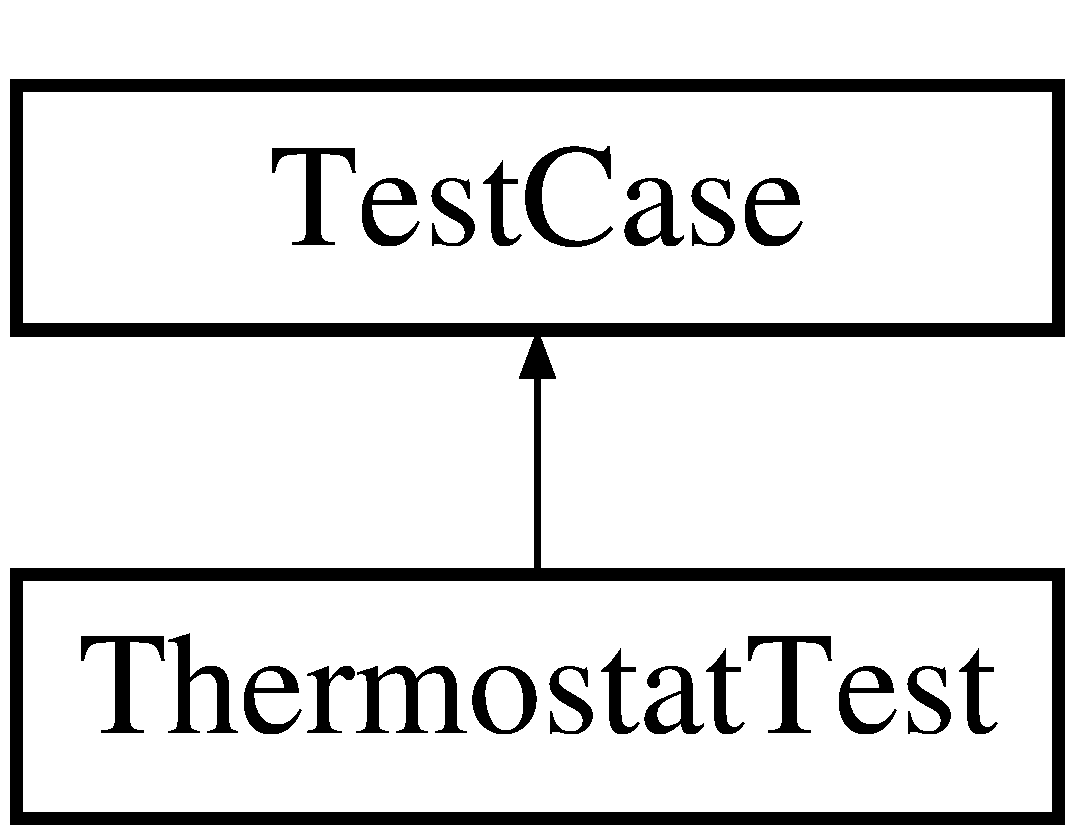
\includegraphics[height=2.000000cm]{classThermostatTest}
\end{center}
\end{figure}
\subsection*{Public Member Functions}
\begin{DoxyCompactItemize}
\item 
\hyperlink{classThermostatTest_ad94e00a85b238de4af9c2f4c5a69e5d3}{Thermostat\-Test} ()
\item 
virtual \hyperlink{classThermostatTest_a88e2ecd8828ff3594f082f76c18f8fbf}{$\sim$\-Thermostat\-Test} ()
\item 
void \hyperlink{classThermostatTest_a7976b8d7def04b6eccde6ff4736e9946}{set\-Up} ()
\item 
void \hyperlink{classThermostatTest_a435da4217dd44255d1f76cdfc1320a9f}{tear\-Down} ()
\item 
void \hyperlink{classThermostatTest_a98768aed0f99becbc3b0f1459f115626}{test\-Default\-Constructor} ()
\item 
void \hyperlink{classThermostatTest_aff27d37c404ecb05ace856389fa09c63}{test\-Get\-E\-Kin} ()
\item 
void \hyperlink{classThermostatTest_afc34add8ce998672f815fb51c34635f2}{test\-Mean\-V} ()
\item 
void \hyperlink{classThermostatTest_a0c9e9d35a6253607e2c43ac666857989}{test\-Set\-Thermo} ()
\end{DoxyCompactItemize}
\subsection*{Static Public Member Functions}
\begin{DoxyCompactItemize}
\item 
static Test $\ast$ \hyperlink{classThermostatTest_ac9e3485b6655fca945ada2eedaf3bcb3}{suite} ()
\end{DoxyCompactItemize}
\subsection*{Private Attributes}
\begin{DoxyCompactItemize}
\item 
std\-::list$<$ \hyperlink{classParticle}{Particle} $\ast$ $>$ \hyperlink{classThermostatTest_a1aff43e47cd1a702ed5116f42a146bdb}{par\-List}
\item 
\hyperlink{classThermostat}{Thermostat} \hyperlink{classThermostatTest_a5fec96185d950a0e916ebe1f399f58c6}{thermo}
\item 
double \hyperlink{classThermostatTest_aacca1bdd524961644e5dd09a6fff63d1}{e\-Kin}
\item 
bool \hyperlink{classThermostatTest_a11bb0e2c5215ea174f7dd2850fe1fdfd}{brownian\-\_\-flag}
\end{DoxyCompactItemize}


\subsection{Constructor \& Destructor Documentation}
\hypertarget{classThermostatTest_ad94e00a85b238de4af9c2f4c5a69e5d3}{\index{Thermostat\-Test@{Thermostat\-Test}!Thermostat\-Test@{Thermostat\-Test}}
\index{Thermostat\-Test@{Thermostat\-Test}!ThermostatTest@{Thermostat\-Test}}
\subsubsection[{Thermostat\-Test}]{\setlength{\rightskip}{0pt plus 5cm}Thermostat\-Test\-::\-Thermostat\-Test (
\begin{DoxyParamCaption}
{}
\end{DoxyParamCaption}
)}}\label{classThermostatTest_ad94e00a85b238de4af9c2f4c5a69e5d3}
\hypertarget{classThermostatTest_a88e2ecd8828ff3594f082f76c18f8fbf}{\index{Thermostat\-Test@{Thermostat\-Test}!$\sim$\-Thermostat\-Test@{$\sim$\-Thermostat\-Test}}
\index{$\sim$\-Thermostat\-Test@{$\sim$\-Thermostat\-Test}!ThermostatTest@{Thermostat\-Test}}
\subsubsection[{$\sim$\-Thermostat\-Test}]{\setlength{\rightskip}{0pt plus 5cm}Thermostat\-Test\-::$\sim$\-Thermostat\-Test (
\begin{DoxyParamCaption}
{}
\end{DoxyParamCaption}
)\hspace{0.3cm}{\ttfamily [virtual]}}}\label{classThermostatTest_a88e2ecd8828ff3594f082f76c18f8fbf}


\subsection{Member Function Documentation}
\hypertarget{classThermostatTest_a7976b8d7def04b6eccde6ff4736e9946}{\index{Thermostat\-Test@{Thermostat\-Test}!set\-Up@{set\-Up}}
\index{set\-Up@{set\-Up}!ThermostatTest@{Thermostat\-Test}}
\subsubsection[{set\-Up}]{\setlength{\rightskip}{0pt plus 5cm}void Thermostat\-Test\-::set\-Up (
\begin{DoxyParamCaption}
{}
\end{DoxyParamCaption}
)}}\label{classThermostatTest_a7976b8d7def04b6eccde6ff4736e9946}
\hypertarget{classThermostatTest_ac9e3485b6655fca945ada2eedaf3bcb3}{\index{Thermostat\-Test@{Thermostat\-Test}!suite@{suite}}
\index{suite@{suite}!ThermostatTest@{Thermostat\-Test}}
\subsubsection[{suite}]{\setlength{\rightskip}{0pt plus 5cm}Cpp\-Unit\-::\-Test $\ast$ Thermostat\-Test\-::suite (
\begin{DoxyParamCaption}
{}
\end{DoxyParamCaption}
)\hspace{0.3cm}{\ttfamily [static]}}}\label{classThermostatTest_ac9e3485b6655fca945ada2eedaf3bcb3}
\hypertarget{classThermostatTest_a435da4217dd44255d1f76cdfc1320a9f}{\index{Thermostat\-Test@{Thermostat\-Test}!tear\-Down@{tear\-Down}}
\index{tear\-Down@{tear\-Down}!ThermostatTest@{Thermostat\-Test}}
\subsubsection[{tear\-Down}]{\setlength{\rightskip}{0pt plus 5cm}void Thermostat\-Test\-::tear\-Down (
\begin{DoxyParamCaption}
{}
\end{DoxyParamCaption}
)}}\label{classThermostatTest_a435da4217dd44255d1f76cdfc1320a9f}
\hypertarget{classThermostatTest_a98768aed0f99becbc3b0f1459f115626}{\index{Thermostat\-Test@{Thermostat\-Test}!test\-Default\-Constructor@{test\-Default\-Constructor}}
\index{test\-Default\-Constructor@{test\-Default\-Constructor}!ThermostatTest@{Thermostat\-Test}}
\subsubsection[{test\-Default\-Constructor}]{\setlength{\rightskip}{0pt plus 5cm}void Thermostat\-Test\-::test\-Default\-Constructor (
\begin{DoxyParamCaption}
{}
\end{DoxyParamCaption}
)}}\label{classThermostatTest_a98768aed0f99becbc3b0f1459f115626}
\hypertarget{classThermostatTest_aff27d37c404ecb05ace856389fa09c63}{\index{Thermostat\-Test@{Thermostat\-Test}!test\-Get\-E\-Kin@{test\-Get\-E\-Kin}}
\index{test\-Get\-E\-Kin@{test\-Get\-E\-Kin}!ThermostatTest@{Thermostat\-Test}}
\subsubsection[{test\-Get\-E\-Kin}]{\setlength{\rightskip}{0pt plus 5cm}void Thermostat\-Test\-::test\-Get\-E\-Kin (
\begin{DoxyParamCaption}
{}
\end{DoxyParamCaption}
)}}\label{classThermostatTest_aff27d37c404ecb05ace856389fa09c63}
\hypertarget{classThermostatTest_afc34add8ce998672f815fb51c34635f2}{\index{Thermostat\-Test@{Thermostat\-Test}!test\-Mean\-V@{test\-Mean\-V}}
\index{test\-Mean\-V@{test\-Mean\-V}!ThermostatTest@{Thermostat\-Test}}
\subsubsection[{test\-Mean\-V}]{\setlength{\rightskip}{0pt plus 5cm}void Thermostat\-Test\-::test\-Mean\-V (
\begin{DoxyParamCaption}
{}
\end{DoxyParamCaption}
)}}\label{classThermostatTest_afc34add8ce998672f815fb51c34635f2}
\hypertarget{classThermostatTest_a0c9e9d35a6253607e2c43ac666857989}{\index{Thermostat\-Test@{Thermostat\-Test}!test\-Set\-Thermo@{test\-Set\-Thermo}}
\index{test\-Set\-Thermo@{test\-Set\-Thermo}!ThermostatTest@{Thermostat\-Test}}
\subsubsection[{test\-Set\-Thermo}]{\setlength{\rightskip}{0pt plus 5cm}void Thermostat\-Test\-::test\-Set\-Thermo (
\begin{DoxyParamCaption}
{}
\end{DoxyParamCaption}
)}}\label{classThermostatTest_a0c9e9d35a6253607e2c43ac666857989}


\subsection{Member Data Documentation}
\hypertarget{classThermostatTest_a11bb0e2c5215ea174f7dd2850fe1fdfd}{\index{Thermostat\-Test@{Thermostat\-Test}!brownian\-\_\-flag@{brownian\-\_\-flag}}
\index{brownian\-\_\-flag@{brownian\-\_\-flag}!ThermostatTest@{Thermostat\-Test}}
\subsubsection[{brownian\-\_\-flag}]{\setlength{\rightskip}{0pt plus 5cm}bool Thermostat\-Test\-::brownian\-\_\-flag\hspace{0.3cm}{\ttfamily [private]}}}\label{classThermostatTest_a11bb0e2c5215ea174f7dd2850fe1fdfd}
\hypertarget{classThermostatTest_aacca1bdd524961644e5dd09a6fff63d1}{\index{Thermostat\-Test@{Thermostat\-Test}!e\-Kin@{e\-Kin}}
\index{e\-Kin@{e\-Kin}!ThermostatTest@{Thermostat\-Test}}
\subsubsection[{e\-Kin}]{\setlength{\rightskip}{0pt plus 5cm}double Thermostat\-Test\-::e\-Kin\hspace{0.3cm}{\ttfamily [private]}}}\label{classThermostatTest_aacca1bdd524961644e5dd09a6fff63d1}
\hypertarget{classThermostatTest_a1aff43e47cd1a702ed5116f42a146bdb}{\index{Thermostat\-Test@{Thermostat\-Test}!par\-List@{par\-List}}
\index{par\-List@{par\-List}!ThermostatTest@{Thermostat\-Test}}
\subsubsection[{par\-List}]{\setlength{\rightskip}{0pt plus 5cm}std\-::list$<${\bf Particle}$\ast$ $>$ Thermostat\-Test\-::par\-List\hspace{0.3cm}{\ttfamily [private]}}}\label{classThermostatTest_a1aff43e47cd1a702ed5116f42a146bdb}
\hypertarget{classThermostatTest_a5fec96185d950a0e916ebe1f399f58c6}{\index{Thermostat\-Test@{Thermostat\-Test}!thermo@{thermo}}
\index{thermo@{thermo}!ThermostatTest@{Thermostat\-Test}}
\subsubsection[{thermo}]{\setlength{\rightskip}{0pt plus 5cm}{\bf Thermostat} Thermostat\-Test\-::thermo\hspace{0.3cm}{\ttfamily [private]}}}\label{classThermostatTest_a5fec96185d950a0e916ebe1f399f58c6}


The documentation for this class was generated from the following files\-:\begin{DoxyCompactItemize}
\item 
src/tests/\hyperlink{ThermostatTest_8h}{Thermostat\-Test.\-h}\item 
src/tests/\hyperlink{ThermostatTest_8cpp}{Thermostat\-Test.\-cpp}\end{DoxyCompactItemize}

\hypertarget{classtype}{\section{type Class Reference}
\label{classtype}\index{type@{type}}
}


Enumeration class corresponding to the type schema type.  




{\ttfamily \#include $<$vtk-\/unstructured.\-h$>$}

Inheritance diagram for type\-:\begin{figure}[H]
\begin{center}
\leavevmode
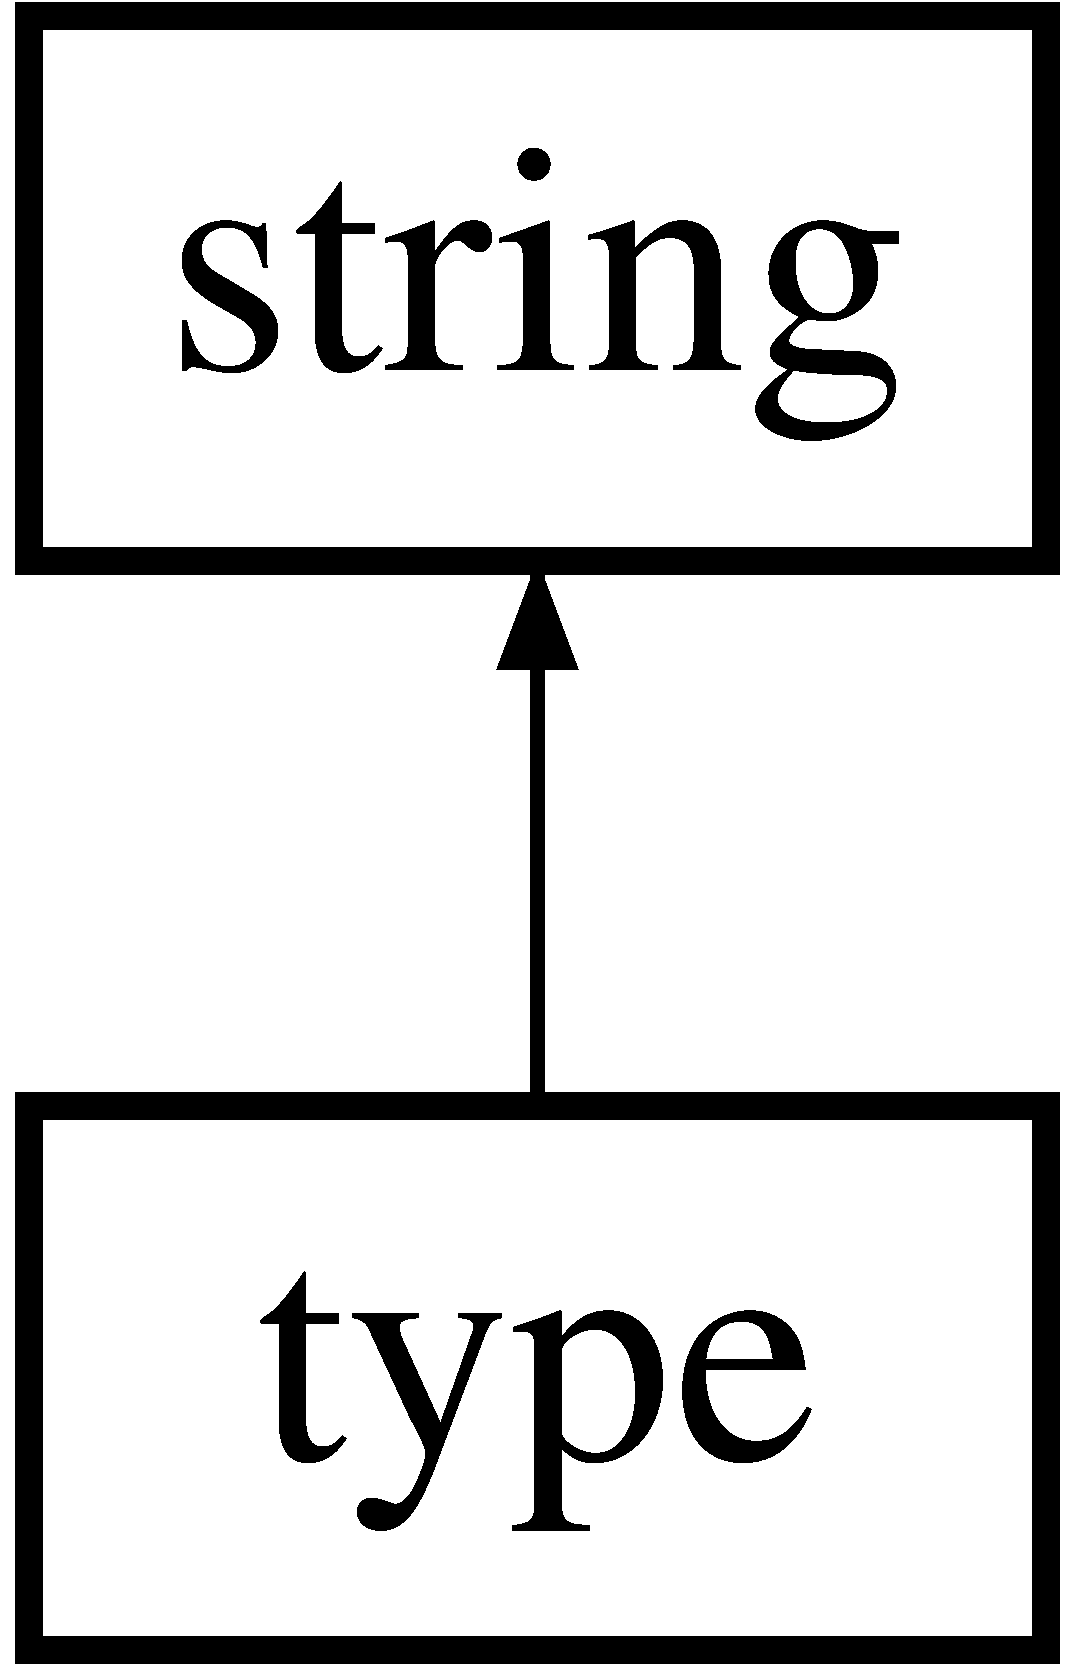
\includegraphics[height=2.000000cm]{classtype}
\end{center}
\end{figure}
\subsection*{Public Types}
\begin{DoxyCompactItemize}
\item 
enum \hyperlink{classtype_a83781d700ce124b4224c316326a5a975}{value} \{ \\*
\hyperlink{classtype_a83781d700ce124b4224c316326a5a975ad559d992c88431b0a1cb90b340929d4e}{Int8}, 
\hyperlink{classtype_a83781d700ce124b4224c316326a5a975a82bbc808c985056ed74b30bcca131fad}{U\-Int8}, 
\hyperlink{classtype_a83781d700ce124b4224c316326a5a975a8d3d044c5da17c4e92e2c61c2f0ea556}{Int16}, 
\hyperlink{classtype_a83781d700ce124b4224c316326a5a975a36b08866238b21675704f38517929e69}{U\-Int16}, 
\\*
\hyperlink{classtype_a83781d700ce124b4224c316326a5a975a62e1ad64aa38ad0b50e1a6bd9b9ae25e}{Int32}, 
\hyperlink{classtype_a83781d700ce124b4224c316326a5a975acfca6c13984dbb7ac515cff88a01826e}{U\-Int32}, 
\hyperlink{classtype_a83781d700ce124b4224c316326a5a975a2cc7bf870db9a3b5e9e580a58b6c1308}{Int64}, 
\hyperlink{classtype_a83781d700ce124b4224c316326a5a975a64538f1914f2fd739bc876253b75fe4c}{U\-Int64}, 
\\*
\hyperlink{classtype_a83781d700ce124b4224c316326a5a975a1b5e448b6fc2bafbc9b5f8e4cc582834}{Float32}, 
\hyperlink{classtype_a83781d700ce124b4224c316326a5a975a72818204734582235e144a1e64563947}{Float64}
 \}
\begin{DoxyCompactList}\small\item\em Underlying enum type. \end{DoxyCompactList}\end{DoxyCompactItemize}
\subsection*{Public Member Functions}
\begin{DoxyCompactItemize}
\item 
\hyperlink{classtype_aed51d13ee609d224084c6cf0a9903f99}{type} (\hyperlink{classtype_a83781d700ce124b4224c316326a5a975}{value} v)
\begin{DoxyCompactList}\small\item\em Create an instance from the underlying enum value. \end{DoxyCompactList}\item 
\hyperlink{classtype_aa5e87da016a56579ba0fc72de17517a5}{type} (const char $\ast$v)
\begin{DoxyCompactList}\small\item\em Create an instance from a C string. \end{DoxyCompactList}\item 
\hyperlink{classtype_ae83bd8bffd0b7251dd664efe908511e7}{type} (const \-::std\-::string \&v)
\begin{DoxyCompactList}\small\item\em Create an instance from a string. \end{DoxyCompactList}\item 
\hyperlink{classtype_a9638b8e282f51d97c9e4e8d703e1f89c}{type} (const \-::\hyperlink{namespacexml__schema_ac0cec83a330f0024e4e318b3deac5104}{xml\-\_\-schema\-::string} \&v)
\begin{DoxyCompactList}\small\item\em Create an instance from the base value. \end{DoxyCompactList}\item 
\hyperlink{classtype_aae224adcb4348cedbe90f4af5dcf1353}{type} (const \-::xercesc\-::\-D\-O\-M\-Element \&e,\-::\hyperlink{namespacexml__schema_a0612287d030cb2732d31a45b258fdc87}{xml\-\_\-schema\-::flags} f=0,\-::\hyperlink{namespacexml__schema_ada9aa30dc722e93ee2ed7243085402a5}{xml\-\_\-schema\-::container} $\ast$c=0)
\begin{DoxyCompactList}\small\item\em Create an instance from a D\-O\-M element. \end{DoxyCompactList}\item 
\hyperlink{classtype_a7018bbc02d3c782aed64822b87dda220}{type} (const \-::xercesc\-::\-D\-O\-M\-Attr \&a,\-::\hyperlink{namespacexml__schema_a0612287d030cb2732d31a45b258fdc87}{xml\-\_\-schema\-::flags} f=0,\-::\hyperlink{namespacexml__schema_ada9aa30dc722e93ee2ed7243085402a5}{xml\-\_\-schema\-::container} $\ast$c=0)
\begin{DoxyCompactList}\small\item\em Create an instance from a D\-O\-M attribute. \end{DoxyCompactList}\item 
\hyperlink{classtype_ac6751e8c63b52e22f73a1ab24d50a082}{type} (const \-::std\-::string \&s, const \-::xercesc\-::\-D\-O\-M\-Element $\ast$e,\-::\hyperlink{namespacexml__schema_a0612287d030cb2732d31a45b258fdc87}{xml\-\_\-schema\-::flags} f=0,\-::\hyperlink{namespacexml__schema_ada9aa30dc722e93ee2ed7243085402a5}{xml\-\_\-schema\-::container} $\ast$c=0)
\begin{DoxyCompactList}\small\item\em Create an instance from a string fragment. \end{DoxyCompactList}\item 
\hyperlink{classtype_aa5eaba8747f76ddbccbb88f68e3311fe}{type} (const \hyperlink{classtype}{type} \&x,\-::\hyperlink{namespacexml__schema_a0612287d030cb2732d31a45b258fdc87}{xml\-\_\-schema\-::flags} f=0,\-::\hyperlink{namespacexml__schema_ada9aa30dc722e93ee2ed7243085402a5}{xml\-\_\-schema\-::container} $\ast$c=0)
\begin{DoxyCompactList}\small\item\em Copy constructor. \end{DoxyCompactList}\item 
virtual \hyperlink{classtype}{type} $\ast$ \hyperlink{classtype_afebbdc11bbf07de7ab79f148e9cd88b6}{\-\_\-clone} (\-::\hyperlink{namespacexml__schema_a0612287d030cb2732d31a45b258fdc87}{xml\-\_\-schema\-::flags} f=0,\-::\hyperlink{namespacexml__schema_ada9aa30dc722e93ee2ed7243085402a5}{xml\-\_\-schema\-::container} $\ast$c=0) const 
\begin{DoxyCompactList}\small\item\em Copy the instance polymorphically. \end{DoxyCompactList}\item 
\hyperlink{classtype}{type} \& \hyperlink{classtype_af55f6d7e02cf92b839d842a58e2911ed}{operator=} (\hyperlink{classtype_a83781d700ce124b4224c316326a5a975}{value} v)
\begin{DoxyCompactList}\small\item\em Assign the underlying enum value. \end{DoxyCompactList}\item 
virtual \hyperlink{classtype_a5bfa60d90029d683cb4e46de45460246}{operator value} () const 
\begin{DoxyCompactList}\small\item\em Implicit conversion operator to the underlying enum value. \end{DoxyCompactList}\end{DoxyCompactItemize}


\subsection{Detailed Description}
Enumeration class corresponding to the type schema type. 

\subsection{Member Enumeration Documentation}
\hypertarget{classtype_a83781d700ce124b4224c316326a5a975}{\index{type@{type}!value@{value}}
\index{value@{value}!type@{type}}
\subsubsection[{value}]{\setlength{\rightskip}{0pt plus 5cm}enum {\bf type\-::value}}}\label{classtype_a83781d700ce124b4224c316326a5a975}


Underlying enum type. 

\begin{Desc}
\item[Enumerator]\par
\begin{description}
\index{Int8@{Int8}!type@{type}}\index{type@{type}!Int8@{Int8}}\item[{\em 
\hypertarget{classtype_a83781d700ce124b4224c316326a5a975ad559d992c88431b0a1cb90b340929d4e}{Int8}\label{classtype_a83781d700ce124b4224c316326a5a975ad559d992c88431b0a1cb90b340929d4e}
}]\index{U\-Int8@{U\-Int8}!type@{type}}\index{type@{type}!U\-Int8@{U\-Int8}}\item[{\em 
\hypertarget{classtype_a83781d700ce124b4224c316326a5a975a82bbc808c985056ed74b30bcca131fad}{U\-Int8}\label{classtype_a83781d700ce124b4224c316326a5a975a82bbc808c985056ed74b30bcca131fad}
}]\index{Int16@{Int16}!type@{type}}\index{type@{type}!Int16@{Int16}}\item[{\em 
\hypertarget{classtype_a83781d700ce124b4224c316326a5a975a8d3d044c5da17c4e92e2c61c2f0ea556}{Int16}\label{classtype_a83781d700ce124b4224c316326a5a975a8d3d044c5da17c4e92e2c61c2f0ea556}
}]\index{U\-Int16@{U\-Int16}!type@{type}}\index{type@{type}!U\-Int16@{U\-Int16}}\item[{\em 
\hypertarget{classtype_a83781d700ce124b4224c316326a5a975a36b08866238b21675704f38517929e69}{U\-Int16}\label{classtype_a83781d700ce124b4224c316326a5a975a36b08866238b21675704f38517929e69}
}]\index{Int32@{Int32}!type@{type}}\index{type@{type}!Int32@{Int32}}\item[{\em 
\hypertarget{classtype_a83781d700ce124b4224c316326a5a975a62e1ad64aa38ad0b50e1a6bd9b9ae25e}{Int32}\label{classtype_a83781d700ce124b4224c316326a5a975a62e1ad64aa38ad0b50e1a6bd9b9ae25e}
}]\index{U\-Int32@{U\-Int32}!type@{type}}\index{type@{type}!U\-Int32@{U\-Int32}}\item[{\em 
\hypertarget{classtype_a83781d700ce124b4224c316326a5a975acfca6c13984dbb7ac515cff88a01826e}{U\-Int32}\label{classtype_a83781d700ce124b4224c316326a5a975acfca6c13984dbb7ac515cff88a01826e}
}]\index{Int64@{Int64}!type@{type}}\index{type@{type}!Int64@{Int64}}\item[{\em 
\hypertarget{classtype_a83781d700ce124b4224c316326a5a975a2cc7bf870db9a3b5e9e580a58b6c1308}{Int64}\label{classtype_a83781d700ce124b4224c316326a5a975a2cc7bf870db9a3b5e9e580a58b6c1308}
}]\index{U\-Int64@{U\-Int64}!type@{type}}\index{type@{type}!U\-Int64@{U\-Int64}}\item[{\em 
\hypertarget{classtype_a83781d700ce124b4224c316326a5a975a64538f1914f2fd739bc876253b75fe4c}{U\-Int64}\label{classtype_a83781d700ce124b4224c316326a5a975a64538f1914f2fd739bc876253b75fe4c}
}]\index{Float32@{Float32}!type@{type}}\index{type@{type}!Float32@{Float32}}\item[{\em 
\hypertarget{classtype_a83781d700ce124b4224c316326a5a975a1b5e448b6fc2bafbc9b5f8e4cc582834}{Float32}\label{classtype_a83781d700ce124b4224c316326a5a975a1b5e448b6fc2bafbc9b5f8e4cc582834}
}]\index{Float64@{Float64}!type@{type}}\index{type@{type}!Float64@{Float64}}\item[{\em 
\hypertarget{classtype_a83781d700ce124b4224c316326a5a975a72818204734582235e144a1e64563947}{Float64}\label{classtype_a83781d700ce124b4224c316326a5a975a72818204734582235e144a1e64563947}
}]\end{description}
\end{Desc}


\subsection{Constructor \& Destructor Documentation}
\hypertarget{classtype_aed51d13ee609d224084c6cf0a9903f99}{\index{type@{type}!type@{type}}
\index{type@{type}!type@{type}}
\subsubsection[{type}]{\setlength{\rightskip}{0pt plus 5cm}type\-::type (
\begin{DoxyParamCaption}
\item[{{\bf value}}]{v}
\end{DoxyParamCaption}
)}}\label{classtype_aed51d13ee609d224084c6cf0a9903f99}


Create an instance from the underlying enum value. 


\begin{DoxyParams}{Parameters}
{\em v} & A enum value. \\
\hline
\end{DoxyParams}
\hypertarget{classtype_aa5e87da016a56579ba0fc72de17517a5}{\index{type@{type}!type@{type}}
\index{type@{type}!type@{type}}
\subsubsection[{type}]{\setlength{\rightskip}{0pt plus 5cm}type\-::type (
\begin{DoxyParamCaption}
\item[{const char $\ast$}]{v}
\end{DoxyParamCaption}
)}}\label{classtype_aa5e87da016a56579ba0fc72de17517a5}


Create an instance from a C string. 


\begin{DoxyParams}{Parameters}
{\em v} & A string value. \\
\hline
\end{DoxyParams}
\hypertarget{classtype_ae83bd8bffd0b7251dd664efe908511e7}{\index{type@{type}!type@{type}}
\index{type@{type}!type@{type}}
\subsubsection[{type}]{\setlength{\rightskip}{0pt plus 5cm}type\-::type (
\begin{DoxyParamCaption}
\item[{const \-::std\-::string \&}]{v}
\end{DoxyParamCaption}
)}}\label{classtype_ae83bd8bffd0b7251dd664efe908511e7}


Create an instance from a string. 


\begin{DoxyParams}{Parameters}
{\em v} & A string value. \\
\hline
\end{DoxyParams}
\hypertarget{classtype_a9638b8e282f51d97c9e4e8d703e1f89c}{\index{type@{type}!type@{type}}
\index{type@{type}!type@{type}}
\subsubsection[{type}]{\setlength{\rightskip}{0pt plus 5cm}type\-::type (
\begin{DoxyParamCaption}
\item[{const \-::{\bf xml\-\_\-schema\-::string} \&}]{v}
\end{DoxyParamCaption}
)}}\label{classtype_a9638b8e282f51d97c9e4e8d703e1f89c}


Create an instance from the base value. 


\begin{DoxyParams}{Parameters}
{\em v} & A base value. \\
\hline
\end{DoxyParams}
\hypertarget{classtype_aae224adcb4348cedbe90f4af5dcf1353}{\index{type@{type}!type@{type}}
\index{type@{type}!type@{type}}
\subsubsection[{type}]{\setlength{\rightskip}{0pt plus 5cm}type\-::type (
\begin{DoxyParamCaption}
\item[{const \-::xercesc\-::\-D\-O\-M\-Element \&}]{e, }
\item[{\-::{\bf xml\-\_\-schema\-::flags}}]{f = {\ttfamily 0}, }
\item[{\-::{\bf xml\-\_\-schema\-::container} $\ast$}]{c = {\ttfamily 0}}
\end{DoxyParamCaption}
)}}\label{classtype_aae224adcb4348cedbe90f4af5dcf1353}


Create an instance from a D\-O\-M element. 


\begin{DoxyParams}{Parameters}
{\em e} & A D\-O\-M element to extract the data from. \\
\hline
{\em f} & Flags to create the new instance with. \\
\hline
{\em c} & A pointer to the object that will contain the new instance. \\
\hline
\end{DoxyParams}
\hypertarget{classtype_a7018bbc02d3c782aed64822b87dda220}{\index{type@{type}!type@{type}}
\index{type@{type}!type@{type}}
\subsubsection[{type}]{\setlength{\rightskip}{0pt plus 5cm}type\-::type (
\begin{DoxyParamCaption}
\item[{const \-::xercesc\-::\-D\-O\-M\-Attr \&}]{a, }
\item[{\-::{\bf xml\-\_\-schema\-::flags}}]{f = {\ttfamily 0}, }
\item[{\-::{\bf xml\-\_\-schema\-::container} $\ast$}]{c = {\ttfamily 0}}
\end{DoxyParamCaption}
)}}\label{classtype_a7018bbc02d3c782aed64822b87dda220}


Create an instance from a D\-O\-M attribute. 


\begin{DoxyParams}{Parameters}
{\em a} & A D\-O\-M attribute to extract the data from. \\
\hline
{\em f} & Flags to create the new instance with. \\
\hline
{\em c} & A pointer to the object that will contain the new instance. \\
\hline
\end{DoxyParams}
\hypertarget{classtype_ac6751e8c63b52e22f73a1ab24d50a082}{\index{type@{type}!type@{type}}
\index{type@{type}!type@{type}}
\subsubsection[{type}]{\setlength{\rightskip}{0pt plus 5cm}type\-::type (
\begin{DoxyParamCaption}
\item[{const \-::std\-::string \&}]{s, }
\item[{const \-::xercesc\-::\-D\-O\-M\-Element $\ast$}]{e, }
\item[{\-::{\bf xml\-\_\-schema\-::flags}}]{f = {\ttfamily 0}, }
\item[{\-::{\bf xml\-\_\-schema\-::container} $\ast$}]{c = {\ttfamily 0}}
\end{DoxyParamCaption}
)}}\label{classtype_ac6751e8c63b52e22f73a1ab24d50a082}


Create an instance from a string fragment. 


\begin{DoxyParams}{Parameters}
{\em s} & A string fragment to extract the data from. \\
\hline
{\em e} & A pointer to D\-O\-M element containing the string fragment. \\
\hline
{\em f} & Flags to create the new instance with. \\
\hline
{\em c} & A pointer to the object that will contain the new instance. \\
\hline
\end{DoxyParams}
\hypertarget{classtype_aa5eaba8747f76ddbccbb88f68e3311fe}{\index{type@{type}!type@{type}}
\index{type@{type}!type@{type}}
\subsubsection[{type}]{\setlength{\rightskip}{0pt plus 5cm}type\-::type (
\begin{DoxyParamCaption}
\item[{const {\bf type} \&}]{x, }
\item[{\-::{\bf xml\-\_\-schema\-::flags}}]{f = {\ttfamily 0}, }
\item[{\-::{\bf xml\-\_\-schema\-::container} $\ast$}]{c = {\ttfamily 0}}
\end{DoxyParamCaption}
)}}\label{classtype_aa5eaba8747f76ddbccbb88f68e3311fe}


Copy constructor. 


\begin{DoxyParams}{Parameters}
{\em x} & An instance to make a copy of. \\
\hline
{\em f} & Flags to create the copy with. \\
\hline
{\em c} & A pointer to the object that will contain the copy.\\
\hline
\end{DoxyParams}
For polymorphic object models use the {\ttfamily \-\_\-clone} function instead. 

\subsection{Member Function Documentation}
\hypertarget{classtype_afebbdc11bbf07de7ab79f148e9cd88b6}{\index{type@{type}!\-\_\-clone@{\-\_\-clone}}
\index{\-\_\-clone@{\-\_\-clone}!type@{type}}
\subsubsection[{\-\_\-clone}]{\setlength{\rightskip}{0pt plus 5cm}{\bf type} $\ast$ type\-::\-\_\-clone (
\begin{DoxyParamCaption}
\item[{\-::{\bf xml\-\_\-schema\-::flags}}]{f = {\ttfamily 0}, }
\item[{\-::{\bf xml\-\_\-schema\-::container} $\ast$}]{c = {\ttfamily 0}}
\end{DoxyParamCaption}
) const\hspace{0.3cm}{\ttfamily [virtual]}}}\label{classtype_afebbdc11bbf07de7ab79f148e9cd88b6}


Copy the instance polymorphically. 


\begin{DoxyParams}{Parameters}
{\em f} & Flags to create the copy with. \\
\hline
{\em c} & A pointer to the object that will contain the copy. \\
\hline
\end{DoxyParams}
\begin{DoxyReturn}{Returns}
A pointer to the dynamically allocated copy.
\end{DoxyReturn}
This function ensures that the dynamic type of the instance is used for copying and should be used for polymorphic object models instead of the copy constructor. \hypertarget{classtype_a5bfa60d90029d683cb4e46de45460246}{\index{type@{type}!operator value@{operator value}}
\index{operator value@{operator value}!type@{type}}
\subsubsection[{operator value}]{\setlength{\rightskip}{0pt plus 5cm}virtual type\-::operator {\bf value} (
\begin{DoxyParamCaption}
{}
\end{DoxyParamCaption}
) const\hspace{0.3cm}{\ttfamily [inline]}, {\ttfamily [virtual]}}}\label{classtype_a5bfa60d90029d683cb4e46de45460246}


Implicit conversion operator to the underlying enum value. 

\begin{DoxyReturn}{Returns}
A enum value. 
\end{DoxyReturn}
\hypertarget{classtype_af55f6d7e02cf92b839d842a58e2911ed}{\index{type@{type}!operator=@{operator=}}
\index{operator=@{operator=}!type@{type}}
\subsubsection[{operator=}]{\setlength{\rightskip}{0pt plus 5cm}{\bf type} \& type\-::operator= (
\begin{DoxyParamCaption}
\item[{{\bf value}}]{v}
\end{DoxyParamCaption}
)}}\label{classtype_af55f6d7e02cf92b839d842a58e2911ed}


Assign the underlying enum value. 


\begin{DoxyParams}{Parameters}
{\em v} & A enum value. \\
\hline
\end{DoxyParams}
\begin{DoxyReturn}{Returns}
A refernce to the instance. 
\end{DoxyReturn}


The documentation for this class was generated from the following files\-:\begin{DoxyCompactItemize}
\item 
src/output\-Writer/\hyperlink{vtk-unstructured_8h}{vtk-\/unstructured.\-h}\item 
src/output\-Writer/\hyperlink{vtk-unstructured_8cpp}{vtk-\/unstructured.\-cpp}\end{DoxyCompactItemize}

\hypertarget{classtype__t}{\section{type\-\_\-t Class Reference}
\label{classtype__t}\index{type\-\_\-t@{type\-\_\-t}}
}


{\ttfamily \#include $<$Input\-Setting.\-h$>$}

Inheritance diagram for type\-\_\-t\-:\begin{figure}[H]
\begin{center}
\leavevmode
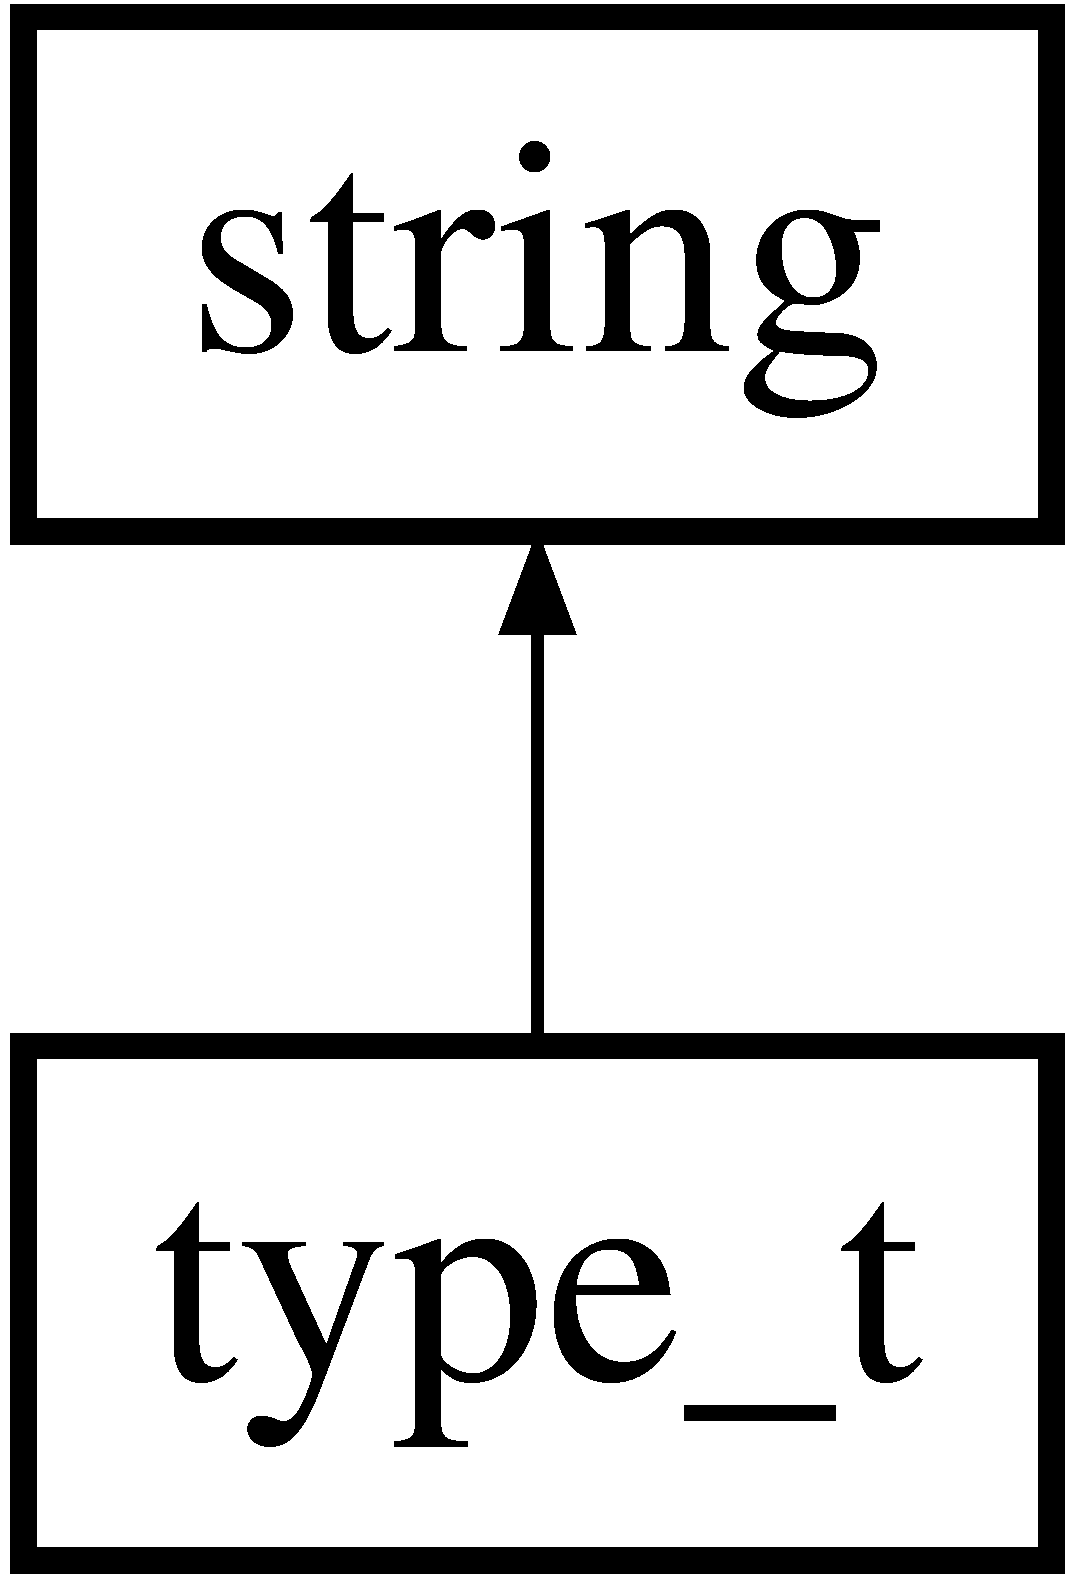
\includegraphics[height=2.000000cm]{classtype__t}
\end{center}
\end{figure}
\subsection*{Public Types}
\begin{DoxyCompactItemize}
\item 
enum \hyperlink{classtype__t_a2cd65d363cac2eb0d81f2e61f5b6bcff}{value} \{ \hyperlink{classtype__t_a2cd65d363cac2eb0d81f2e61f5b6bcffa409d3782b4f6927afcc69102658ed168}{cuboids}, 
\hyperlink{classtype__t_a2cd65d363cac2eb0d81f2e61f5b6bcffa05a7bd0ffe485d63238c8662602324fd}{particles}, 
\hyperlink{classtype__t_a2cd65d363cac2eb0d81f2e61f5b6bcffa7d69ee9ff344652e998bbe551581ab24}{spheres}
 \}
\end{DoxyCompactItemize}
\subsection*{Public Member Functions}
\begin{DoxyCompactItemize}
\item 
\hyperlink{classtype__t_aef3e1ffc719f81b6e64dfc82d3e68fb4}{type\-\_\-t} (\hyperlink{classtype__t_a2cd65d363cac2eb0d81f2e61f5b6bcff}{value} v)
\item 
\hyperlink{classtype__t_a25df0d2d77574789bf604d129d97628f}{type\-\_\-t} (const char $\ast$v)
\item 
\hyperlink{classtype__t_a9a28b05c320cda87aa8a4e983e23ab3a}{type\-\_\-t} (const \-::std\-::string \&v)
\item 
\hyperlink{classtype__t_a4e0bc111a2870ce6751bcf7853f85f77}{type\-\_\-t} (const \-::\hyperlink{namespacexml__schema_ac0cec83a330f0024e4e318b3deac5104}{xml\-\_\-schema\-::string} \&v)
\item 
\hyperlink{classtype__t_a63e1768303f3920d245c2560979c2448}{type\-\_\-t} (const \-::xercesc\-::\-D\-O\-M\-Element \&e,\-::\hyperlink{namespacexml__schema_a0612287d030cb2732d31a45b258fdc87}{xml\-\_\-schema\-::flags} f=0,\-::\hyperlink{namespacexml__schema_ada9aa30dc722e93ee2ed7243085402a5}{xml\-\_\-schema\-::container} $\ast$c=0)
\item 
\hyperlink{classtype__t_a85e514cc4d8c9aaa43fb780d4d1cdea8}{type\-\_\-t} (const \-::xercesc\-::\-D\-O\-M\-Attr \&a,\-::\hyperlink{namespacexml__schema_a0612287d030cb2732d31a45b258fdc87}{xml\-\_\-schema\-::flags} f=0,\-::\hyperlink{namespacexml__schema_ada9aa30dc722e93ee2ed7243085402a5}{xml\-\_\-schema\-::container} $\ast$c=0)
\item 
\hyperlink{classtype__t_af6fbe42125b54356daaf31ab4aff7831}{type\-\_\-t} (const \-::std\-::string \&s, const \-::xercesc\-::\-D\-O\-M\-Element $\ast$e,\-::\hyperlink{namespacexml__schema_a0612287d030cb2732d31a45b258fdc87}{xml\-\_\-schema\-::flags} f=0,\-::\hyperlink{namespacexml__schema_ada9aa30dc722e93ee2ed7243085402a5}{xml\-\_\-schema\-::container} $\ast$c=0)
\item 
\hyperlink{classtype__t_aa021e327a8ab0832078768e33cf794f9}{type\-\_\-t} (const \hyperlink{classtype__t}{type\-\_\-t} \&x,\-::\hyperlink{namespacexml__schema_a0612287d030cb2732d31a45b258fdc87}{xml\-\_\-schema\-::flags} f=0,\-::\hyperlink{namespacexml__schema_ada9aa30dc722e93ee2ed7243085402a5}{xml\-\_\-schema\-::container} $\ast$c=0)
\item 
virtual \hyperlink{classtype__t}{type\-\_\-t} $\ast$ \hyperlink{classtype__t_a0e130a014f1dec009183e9aa812db836}{\-\_\-clone} (\-::\hyperlink{namespacexml__schema_a0612287d030cb2732d31a45b258fdc87}{xml\-\_\-schema\-::flags} f=0,\-::\hyperlink{namespacexml__schema_ada9aa30dc722e93ee2ed7243085402a5}{xml\-\_\-schema\-::container} $\ast$c=0) const 
\item 
\hyperlink{classtype__t}{type\-\_\-t} \& \hyperlink{classtype__t_a891cac5504129725bbfb0930cdebae1d}{operator=} (\hyperlink{classtype__t_a2cd65d363cac2eb0d81f2e61f5b6bcff}{value} v)
\item 
virtual \hyperlink{classtype__t_ac7d7e7922ca4fd492aa55851fe8fcf17}{operator value} () const 
\end{DoxyCompactItemize}
\subsection*{Static Public Attributes}
\begin{DoxyCompactItemize}
\item 
static const char $\ast$const \hyperlink{classtype__t_a705db5b354830eabddfc3cca4f622943}{\-\_\-xsd\-\_\-type\-\_\-t\-\_\-literals\-\_\-} \mbox{[}3\mbox{]}
\item 
static const \hyperlink{classtype__t_a2cd65d363cac2eb0d81f2e61f5b6bcff}{value} \hyperlink{classtype__t_a6d98249ea91d2df2401b34eb2f0adda2}{\-\_\-xsd\-\_\-type\-\_\-t\-\_\-indexes\-\_\-} \mbox{[}3\mbox{]}
\end{DoxyCompactItemize}
\subsection*{Protected Member Functions}
\begin{DoxyCompactItemize}
\item 
\hyperlink{classtype__t_a2cd65d363cac2eb0d81f2e61f5b6bcff}{value} \hyperlink{classtype__t_a13952c06b27bc7479c1bdc24cb1a9939}{\-\_\-xsd\-\_\-type\-\_\-t\-\_\-convert} () const 
\end{DoxyCompactItemize}


\subsection{Member Enumeration Documentation}
\hypertarget{classtype__t_a2cd65d363cac2eb0d81f2e61f5b6bcff}{\index{type\-\_\-t@{type\-\_\-t}!value@{value}}
\index{value@{value}!type_t@{type\-\_\-t}}
\subsubsection[{value}]{\setlength{\rightskip}{0pt plus 5cm}enum {\bf type\-\_\-t\-::value}}}\label{classtype__t_a2cd65d363cac2eb0d81f2e61f5b6bcff}
\begin{Desc}
\item[Enumerator]\par
\begin{description}
\index{cuboids@{cuboids}!type\-\_\-t@{type\-\_\-t}}\index{type\-\_\-t@{type\-\_\-t}!cuboids@{cuboids}}\item[{\em 
\hypertarget{classtype__t_a2cd65d363cac2eb0d81f2e61f5b6bcffa409d3782b4f6927afcc69102658ed168}{cuboids}\label{classtype__t_a2cd65d363cac2eb0d81f2e61f5b6bcffa409d3782b4f6927afcc69102658ed168}
}]\index{particles@{particles}!type\-\_\-t@{type\-\_\-t}}\index{type\-\_\-t@{type\-\_\-t}!particles@{particles}}\item[{\em 
\hypertarget{classtype__t_a2cd65d363cac2eb0d81f2e61f5b6bcffa05a7bd0ffe485d63238c8662602324fd}{particles}\label{classtype__t_a2cd65d363cac2eb0d81f2e61f5b6bcffa05a7bd0ffe485d63238c8662602324fd}
}]\index{spheres@{spheres}!type\-\_\-t@{type\-\_\-t}}\index{type\-\_\-t@{type\-\_\-t}!spheres@{spheres}}\item[{\em 
\hypertarget{classtype__t_a2cd65d363cac2eb0d81f2e61f5b6bcffa7d69ee9ff344652e998bbe551581ab24}{spheres}\label{classtype__t_a2cd65d363cac2eb0d81f2e61f5b6bcffa7d69ee9ff344652e998bbe551581ab24}
}]\end{description}
\end{Desc}


\subsection{Constructor \& Destructor Documentation}
\hypertarget{classtype__t_aef3e1ffc719f81b6e64dfc82d3e68fb4}{\index{type\-\_\-t@{type\-\_\-t}!type\-\_\-t@{type\-\_\-t}}
\index{type\-\_\-t@{type\-\_\-t}!type_t@{type\-\_\-t}}
\subsubsection[{type\-\_\-t}]{\setlength{\rightskip}{0pt plus 5cm}type\-\_\-t\-::type\-\_\-t (
\begin{DoxyParamCaption}
\item[{{\bf value}}]{v}
\end{DoxyParamCaption}
)}}\label{classtype__t_aef3e1ffc719f81b6e64dfc82d3e68fb4}
\hypertarget{classtype__t_a25df0d2d77574789bf604d129d97628f}{\index{type\-\_\-t@{type\-\_\-t}!type\-\_\-t@{type\-\_\-t}}
\index{type\-\_\-t@{type\-\_\-t}!type_t@{type\-\_\-t}}
\subsubsection[{type\-\_\-t}]{\setlength{\rightskip}{0pt plus 5cm}type\-\_\-t\-::type\-\_\-t (
\begin{DoxyParamCaption}
\item[{const char $\ast$}]{v}
\end{DoxyParamCaption}
)}}\label{classtype__t_a25df0d2d77574789bf604d129d97628f}
\hypertarget{classtype__t_a9a28b05c320cda87aa8a4e983e23ab3a}{\index{type\-\_\-t@{type\-\_\-t}!type\-\_\-t@{type\-\_\-t}}
\index{type\-\_\-t@{type\-\_\-t}!type_t@{type\-\_\-t}}
\subsubsection[{type\-\_\-t}]{\setlength{\rightskip}{0pt plus 5cm}type\-\_\-t\-::type\-\_\-t (
\begin{DoxyParamCaption}
\item[{const \-::std\-::string \&}]{v}
\end{DoxyParamCaption}
)}}\label{classtype__t_a9a28b05c320cda87aa8a4e983e23ab3a}
\hypertarget{classtype__t_a4e0bc111a2870ce6751bcf7853f85f77}{\index{type\-\_\-t@{type\-\_\-t}!type\-\_\-t@{type\-\_\-t}}
\index{type\-\_\-t@{type\-\_\-t}!type_t@{type\-\_\-t}}
\subsubsection[{type\-\_\-t}]{\setlength{\rightskip}{0pt plus 5cm}type\-\_\-t\-::type\-\_\-t (
\begin{DoxyParamCaption}
\item[{const \-::{\bf xml\-\_\-schema\-::string} \&}]{v}
\end{DoxyParamCaption}
)}}\label{classtype__t_a4e0bc111a2870ce6751bcf7853f85f77}
\hypertarget{classtype__t_a63e1768303f3920d245c2560979c2448}{\index{type\-\_\-t@{type\-\_\-t}!type\-\_\-t@{type\-\_\-t}}
\index{type\-\_\-t@{type\-\_\-t}!type_t@{type\-\_\-t}}
\subsubsection[{type\-\_\-t}]{\setlength{\rightskip}{0pt plus 5cm}type\-\_\-t\-::type\-\_\-t (
\begin{DoxyParamCaption}
\item[{const \-::xercesc\-::\-D\-O\-M\-Element \&}]{e, }
\item[{\-::{\bf xml\-\_\-schema\-::flags}}]{f = {\ttfamily 0}, }
\item[{\-::{\bf xml\-\_\-schema\-::container} $\ast$}]{c = {\ttfamily 0}}
\end{DoxyParamCaption}
)}}\label{classtype__t_a63e1768303f3920d245c2560979c2448}
\hypertarget{classtype__t_a85e514cc4d8c9aaa43fb780d4d1cdea8}{\index{type\-\_\-t@{type\-\_\-t}!type\-\_\-t@{type\-\_\-t}}
\index{type\-\_\-t@{type\-\_\-t}!type_t@{type\-\_\-t}}
\subsubsection[{type\-\_\-t}]{\setlength{\rightskip}{0pt plus 5cm}type\-\_\-t\-::type\-\_\-t (
\begin{DoxyParamCaption}
\item[{const \-::xercesc\-::\-D\-O\-M\-Attr \&}]{a, }
\item[{\-::{\bf xml\-\_\-schema\-::flags}}]{f = {\ttfamily 0}, }
\item[{\-::{\bf xml\-\_\-schema\-::container} $\ast$}]{c = {\ttfamily 0}}
\end{DoxyParamCaption}
)}}\label{classtype__t_a85e514cc4d8c9aaa43fb780d4d1cdea8}
\hypertarget{classtype__t_af6fbe42125b54356daaf31ab4aff7831}{\index{type\-\_\-t@{type\-\_\-t}!type\-\_\-t@{type\-\_\-t}}
\index{type\-\_\-t@{type\-\_\-t}!type_t@{type\-\_\-t}}
\subsubsection[{type\-\_\-t}]{\setlength{\rightskip}{0pt plus 5cm}type\-\_\-t\-::type\-\_\-t (
\begin{DoxyParamCaption}
\item[{const \-::std\-::string \&}]{s, }
\item[{const \-::xercesc\-::\-D\-O\-M\-Element $\ast$}]{e, }
\item[{\-::{\bf xml\-\_\-schema\-::flags}}]{f = {\ttfamily 0}, }
\item[{\-::{\bf xml\-\_\-schema\-::container} $\ast$}]{c = {\ttfamily 0}}
\end{DoxyParamCaption}
)}}\label{classtype__t_af6fbe42125b54356daaf31ab4aff7831}
\hypertarget{classtype__t_aa021e327a8ab0832078768e33cf794f9}{\index{type\-\_\-t@{type\-\_\-t}!type\-\_\-t@{type\-\_\-t}}
\index{type\-\_\-t@{type\-\_\-t}!type_t@{type\-\_\-t}}
\subsubsection[{type\-\_\-t}]{\setlength{\rightskip}{0pt plus 5cm}type\-\_\-t\-::type\-\_\-t (
\begin{DoxyParamCaption}
\item[{const {\bf type\-\_\-t} \&}]{x, }
\item[{\-::{\bf xml\-\_\-schema\-::flags}}]{f = {\ttfamily 0}, }
\item[{\-::{\bf xml\-\_\-schema\-::container} $\ast$}]{c = {\ttfamily 0}}
\end{DoxyParamCaption}
)}}\label{classtype__t_aa021e327a8ab0832078768e33cf794f9}


\subsection{Member Function Documentation}
\hypertarget{classtype__t_a0e130a014f1dec009183e9aa812db836}{\index{type\-\_\-t@{type\-\_\-t}!\-\_\-clone@{\-\_\-clone}}
\index{\-\_\-clone@{\-\_\-clone}!type_t@{type\-\_\-t}}
\subsubsection[{\-\_\-clone}]{\setlength{\rightskip}{0pt plus 5cm}{\bf type\-\_\-t} $\ast$ type\-\_\-t\-::\-\_\-clone (
\begin{DoxyParamCaption}
\item[{\-::{\bf xml\-\_\-schema\-::flags}}]{f = {\ttfamily 0}, }
\item[{\-::{\bf xml\-\_\-schema\-::container} $\ast$}]{c = {\ttfamily 0}}
\end{DoxyParamCaption}
) const\hspace{0.3cm}{\ttfamily [virtual]}}}\label{classtype__t_a0e130a014f1dec009183e9aa812db836}
\hypertarget{classtype__t_a13952c06b27bc7479c1bdc24cb1a9939}{\index{type\-\_\-t@{type\-\_\-t}!\-\_\-xsd\-\_\-type\-\_\-t\-\_\-convert@{\-\_\-xsd\-\_\-type\-\_\-t\-\_\-convert}}
\index{\-\_\-xsd\-\_\-type\-\_\-t\-\_\-convert@{\-\_\-xsd\-\_\-type\-\_\-t\-\_\-convert}!type_t@{type\-\_\-t}}
\subsubsection[{\-\_\-xsd\-\_\-type\-\_\-t\-\_\-convert}]{\setlength{\rightskip}{0pt plus 5cm}{\bf type\-\_\-t\-::value} type\-\_\-t\-::\-\_\-xsd\-\_\-type\-\_\-t\-\_\-convert (
\begin{DoxyParamCaption}
{}
\end{DoxyParamCaption}
) const\hspace{0.3cm}{\ttfamily [protected]}}}\label{classtype__t_a13952c06b27bc7479c1bdc24cb1a9939}
\hypertarget{classtype__t_ac7d7e7922ca4fd492aa55851fe8fcf17}{\index{type\-\_\-t@{type\-\_\-t}!operator value@{operator value}}
\index{operator value@{operator value}!type_t@{type\-\_\-t}}
\subsubsection[{operator value}]{\setlength{\rightskip}{0pt plus 5cm}virtual type\-\_\-t\-::operator {\bf value} (
\begin{DoxyParamCaption}
{}
\end{DoxyParamCaption}
) const\hspace{0.3cm}{\ttfamily [inline]}, {\ttfamily [virtual]}}}\label{classtype__t_ac7d7e7922ca4fd492aa55851fe8fcf17}
\hypertarget{classtype__t_a891cac5504129725bbfb0930cdebae1d}{\index{type\-\_\-t@{type\-\_\-t}!operator=@{operator=}}
\index{operator=@{operator=}!type_t@{type\-\_\-t}}
\subsubsection[{operator=}]{\setlength{\rightskip}{0pt plus 5cm}{\bf type\-\_\-t} \& type\-\_\-t\-::operator= (
\begin{DoxyParamCaption}
\item[{{\bf value}}]{v}
\end{DoxyParamCaption}
)}}\label{classtype__t_a891cac5504129725bbfb0930cdebae1d}


\subsection{Member Data Documentation}
\hypertarget{classtype__t_a6d98249ea91d2df2401b34eb2f0adda2}{\index{type\-\_\-t@{type\-\_\-t}!\-\_\-xsd\-\_\-type\-\_\-t\-\_\-indexes\-\_\-@{\-\_\-xsd\-\_\-type\-\_\-t\-\_\-indexes\-\_\-}}
\index{\-\_\-xsd\-\_\-type\-\_\-t\-\_\-indexes\-\_\-@{\-\_\-xsd\-\_\-type\-\_\-t\-\_\-indexes\-\_\-}!type_t@{type\-\_\-t}}
\subsubsection[{\-\_\-xsd\-\_\-type\-\_\-t\-\_\-indexes\-\_\-}]{\setlength{\rightskip}{0pt plus 5cm}const {\bf type\-\_\-t\-::value} type\-\_\-t\-::\-\_\-xsd\-\_\-type\-\_\-t\-\_\-indexes\-\_\-\hspace{0.3cm}{\ttfamily [static]}}}\label{classtype__t_a6d98249ea91d2df2401b34eb2f0adda2}
{\bfseries Initial value\-:}
\begin{DoxyCode}
=
\{
  \hyperlink{classtype__t_a2cd65d363cac2eb0d81f2e61f5b6bcffa409d3782b4f6927afcc69102658ed168}{::type\_t::cuboids},
  \hyperlink{classtype__t_a2cd65d363cac2eb0d81f2e61f5b6bcffa05a7bd0ffe485d63238c8662602324fd}{::type\_t::particles},
  \hyperlink{classtype__t_a2cd65d363cac2eb0d81f2e61f5b6bcffa7d69ee9ff344652e998bbe551581ab24}{::type\_t::spheres}
\}
\end{DoxyCode}
\hypertarget{classtype__t_a705db5b354830eabddfc3cca4f622943}{\index{type\-\_\-t@{type\-\_\-t}!\-\_\-xsd\-\_\-type\-\_\-t\-\_\-literals\-\_\-@{\-\_\-xsd\-\_\-type\-\_\-t\-\_\-literals\-\_\-}}
\index{\-\_\-xsd\-\_\-type\-\_\-t\-\_\-literals\-\_\-@{\-\_\-xsd\-\_\-type\-\_\-t\-\_\-literals\-\_\-}!type_t@{type\-\_\-t}}
\subsubsection[{\-\_\-xsd\-\_\-type\-\_\-t\-\_\-literals\-\_\-}]{\setlength{\rightskip}{0pt plus 5cm}const char $\ast$const type\-\_\-t\-::\-\_\-xsd\-\_\-type\-\_\-t\-\_\-literals\-\_\-\hspace{0.3cm}{\ttfamily [static]}}}\label{classtype__t_a705db5b354830eabddfc3cca4f622943}
{\bfseries Initial value\-:}
\begin{DoxyCode}
=
\{
  \textcolor{stringliteral}{"cuboids"},
  \textcolor{stringliteral}{"particles"},
  \textcolor{stringliteral}{"spheres"}
\}
\end{DoxyCode}


The documentation for this class was generated from the following files\-:\begin{DoxyCompactItemize}
\item 
src/utils/\hyperlink{InputSetting_8h}{Input\-Setting.\-h}\item 
src/utils/\hyperlink{InputSetting_8cpp}{Input\-Setting.\-cpp}\end{DoxyCompactItemize}

\hypertarget{classUnstructuredGrid__t}{\section{Unstructured\-Grid\-\_\-t Class Reference}
\label{classUnstructuredGrid__t}\index{Unstructured\-Grid\-\_\-t@{Unstructured\-Grid\-\_\-t}}
}


Class corresponding to the Unstructured\-Grid\-\_\-t schema type.  




{\ttfamily \#include $<$vtk-\/unstructured.\-h$>$}

Inheritance diagram for Unstructured\-Grid\-\_\-t\-:\begin{figure}[H]
\begin{center}
\leavevmode
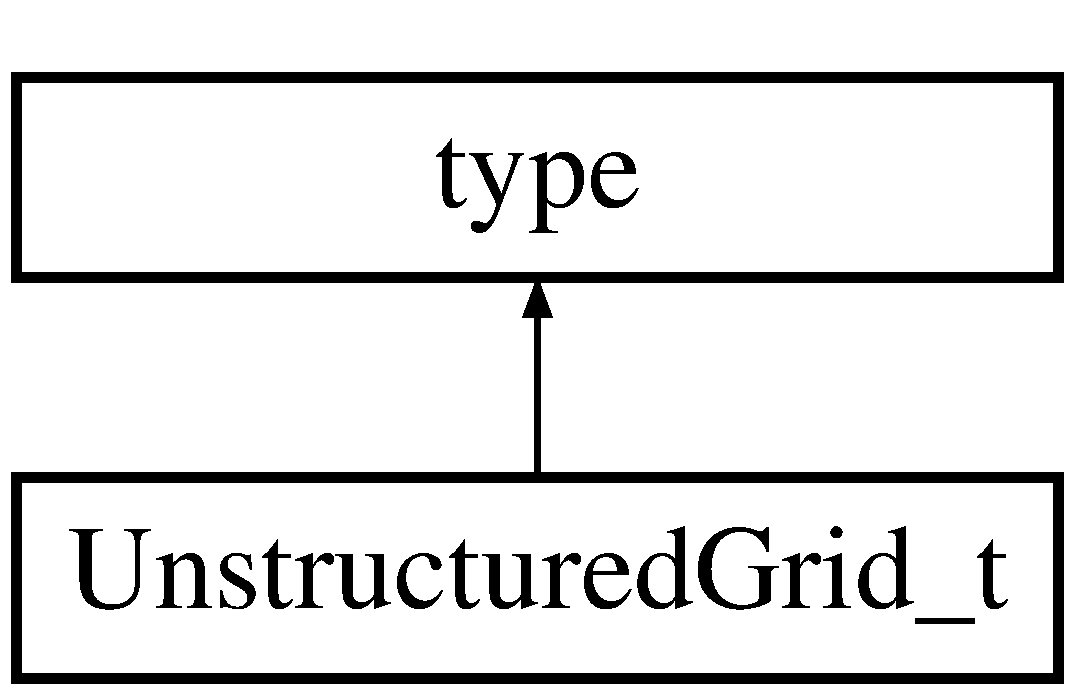
\includegraphics[height=2.000000cm]{classUnstructuredGrid__t}
\end{center}
\end{figure}
\subsection*{Public Member Functions}
\begin{DoxyCompactItemize}
\item 
virtual \hyperlink{classUnstructuredGrid__t_a6fb9239ab1215edd7e7822a66d3af53c}{$\sim$\-Unstructured\-Grid\-\_\-t} ()
\begin{DoxyCompactList}\small\item\em Destructor. \end{DoxyCompactList}\end{DoxyCompactItemize}
\subsection*{Piece}
\label{_amgrpa5d512bf83495b68d0ffa20f79804dfc}%
Accessor and modifier functions for the Piece required element. \begin{DoxyCompactItemize}
\item 
typedef \-::\hyperlink{classPieceUnstructuredGrid__t}{Piece\-Unstructured\-Grid\-\_\-t} \hyperlink{classUnstructuredGrid__t_a559913611314b34f4868027fc91e35bc}{Piece\-\_\-type}
\begin{DoxyCompactList}\small\item\em Element type. \end{DoxyCompactList}\item 
typedef \\*
\-::xsd\-::cxx\-::tree\-::traits\\*
$<$ \hyperlink{classUnstructuredGrid__t_a559913611314b34f4868027fc91e35bc}{Piece\-\_\-type}, char $>$ \hyperlink{classUnstructuredGrid__t_a8a9bf012c364a5fbb78aac9a319a4dad}{Piece\-\_\-traits}
\begin{DoxyCompactList}\small\item\em Element traits type. \end{DoxyCompactList}\item 
const \hyperlink{classUnstructuredGrid__t_a559913611314b34f4868027fc91e35bc}{Piece\-\_\-type} \& \hyperlink{classUnstructuredGrid__t_a32fdd47d79cfdd2eb071cf674b7cc9ee}{Piece} () const 
\begin{DoxyCompactList}\small\item\em Return a read-\/only (constant) reference to the element. \end{DoxyCompactList}\item 
\hyperlink{classUnstructuredGrid__t_a559913611314b34f4868027fc91e35bc}{Piece\-\_\-type} \& \hyperlink{classUnstructuredGrid__t_a66b7c6fc204fdc78b4611fd132771573}{Piece} ()
\begin{DoxyCompactList}\small\item\em Return a read-\/write reference to the element. \end{DoxyCompactList}\item 
void \hyperlink{classUnstructuredGrid__t_a97ef3f79738631a4265c4fbeb170f04d}{Piece} (const \hyperlink{classUnstructuredGrid__t_a559913611314b34f4868027fc91e35bc}{Piece\-\_\-type} \&x)
\begin{DoxyCompactList}\small\item\em Set the element value. \end{DoxyCompactList}\item 
void \hyperlink{classUnstructuredGrid__t_aadd93b1b259778a8ef49c3d6e5b0be5d}{Piece} (\-::std\-::auto\-\_\-ptr$<$ \hyperlink{classUnstructuredGrid__t_a559913611314b34f4868027fc91e35bc}{Piece\-\_\-type} $>$ p)
\begin{DoxyCompactList}\small\item\em Set the element value without copying. \end{DoxyCompactList}\end{DoxyCompactItemize}
\subsection*{Constructors}
\begin{DoxyCompactItemize}
\item 
\hyperlink{classUnstructuredGrid__t_a00bf6957ea7e3313e2890bd4c02f8981}{Unstructured\-Grid\-\_\-t} (const \hyperlink{classUnstructuredGrid__t_a559913611314b34f4868027fc91e35bc}{Piece\-\_\-type} \&)
\begin{DoxyCompactList}\small\item\em Create an instance from the ultimate base and initializers for required elements and attributes. \end{DoxyCompactList}\item 
\hyperlink{classUnstructuredGrid__t_a528c5e53cac3c45f9e5a2ff37197d1c8}{Unstructured\-Grid\-\_\-t} (\-::std\-::auto\-\_\-ptr$<$ \hyperlink{classUnstructuredGrid__t_a559913611314b34f4868027fc91e35bc}{Piece\-\_\-type} $>$ \&)
\begin{DoxyCompactList}\small\item\em Create an instance from the ultimate base and initializers for required elements and attributes (auto\-\_\-ptr version). \end{DoxyCompactList}\item 
\hyperlink{classUnstructuredGrid__t_ad6fb3d97ad8d9443d53e1152a9fa6004}{Unstructured\-Grid\-\_\-t} (const \-::xercesc\-::\-D\-O\-M\-Element \&e,\-::\hyperlink{namespacexml__schema_a0612287d030cb2732d31a45b258fdc87}{xml\-\_\-schema\-::flags} f=0,\-::\hyperlink{namespacexml__schema_ada9aa30dc722e93ee2ed7243085402a5}{xml\-\_\-schema\-::container} $\ast$c=0)
\begin{DoxyCompactList}\small\item\em Create an instance from a D\-O\-M element. \end{DoxyCompactList}\item 
\hyperlink{classUnstructuredGrid__t_a893b6debad8369f36a3cdc2aaa22b478}{Unstructured\-Grid\-\_\-t} (const \hyperlink{classUnstructuredGrid__t}{Unstructured\-Grid\-\_\-t} \&x,\-::\hyperlink{namespacexml__schema_a0612287d030cb2732d31a45b258fdc87}{xml\-\_\-schema\-::flags} f=0,\-::\hyperlink{namespacexml__schema_ada9aa30dc722e93ee2ed7243085402a5}{xml\-\_\-schema\-::container} $\ast$c=0)
\begin{DoxyCompactList}\small\item\em Copy constructor. \end{DoxyCompactList}\item 
virtual \hyperlink{classUnstructuredGrid__t}{Unstructured\-Grid\-\_\-t} $\ast$ \hyperlink{classUnstructuredGrid__t_ae51f374b8650e990f30723bdcf181f2d}{\-\_\-clone} (\-::\hyperlink{namespacexml__schema_a0612287d030cb2732d31a45b258fdc87}{xml\-\_\-schema\-::flags} f=0,\-::\hyperlink{namespacexml__schema_ada9aa30dc722e93ee2ed7243085402a5}{xml\-\_\-schema\-::container} $\ast$c=0) const 
\begin{DoxyCompactList}\small\item\em Copy the instance polymorphically. \end{DoxyCompactList}\end{DoxyCompactItemize}


\subsection{Detailed Description}
Class corresponding to the Unstructured\-Grid\-\_\-t schema type. 

\subsection{Member Typedef Documentation}
\hypertarget{classUnstructuredGrid__t_a8a9bf012c364a5fbb78aac9a319a4dad}{\index{Unstructured\-Grid\-\_\-t@{Unstructured\-Grid\-\_\-t}!Piece\-\_\-traits@{Piece\-\_\-traits}}
\index{Piece\-\_\-traits@{Piece\-\_\-traits}!UnstructuredGrid_t@{Unstructured\-Grid\-\_\-t}}
\subsubsection[{Piece\-\_\-traits}]{\setlength{\rightskip}{0pt plus 5cm}typedef \-::xsd\-::cxx\-::tree\-::traits$<$ {\bf Piece\-\_\-type}, char $>$ {\bf Unstructured\-Grid\-\_\-t\-::\-Piece\-\_\-traits}}}\label{classUnstructuredGrid__t_a8a9bf012c364a5fbb78aac9a319a4dad}


Element traits type. 

\hypertarget{classUnstructuredGrid__t_a559913611314b34f4868027fc91e35bc}{\index{Unstructured\-Grid\-\_\-t@{Unstructured\-Grid\-\_\-t}!Piece\-\_\-type@{Piece\-\_\-type}}
\index{Piece\-\_\-type@{Piece\-\_\-type}!UnstructuredGrid_t@{Unstructured\-Grid\-\_\-t}}
\subsubsection[{Piece\-\_\-type}]{\setlength{\rightskip}{0pt plus 5cm}typedef \-::{\bf Piece\-Unstructured\-Grid\-\_\-t} {\bf Unstructured\-Grid\-\_\-t\-::\-Piece\-\_\-type}}}\label{classUnstructuredGrid__t_a559913611314b34f4868027fc91e35bc}


Element type. 



\subsection{Constructor \& Destructor Documentation}
\hypertarget{classUnstructuredGrid__t_a00bf6957ea7e3313e2890bd4c02f8981}{\index{Unstructured\-Grid\-\_\-t@{Unstructured\-Grid\-\_\-t}!Unstructured\-Grid\-\_\-t@{Unstructured\-Grid\-\_\-t}}
\index{Unstructured\-Grid\-\_\-t@{Unstructured\-Grid\-\_\-t}!UnstructuredGrid_t@{Unstructured\-Grid\-\_\-t}}
\subsubsection[{Unstructured\-Grid\-\_\-t}]{\setlength{\rightskip}{0pt plus 5cm}Unstructured\-Grid\-\_\-t\-::\-Unstructured\-Grid\-\_\-t (
\begin{DoxyParamCaption}
\item[{const {\bf Piece\-\_\-type} \&}]{Piece}
\end{DoxyParamCaption}
)}}\label{classUnstructuredGrid__t_a00bf6957ea7e3313e2890bd4c02f8981}


Create an instance from the ultimate base and initializers for required elements and attributes. 

\hypertarget{classUnstructuredGrid__t_a528c5e53cac3c45f9e5a2ff37197d1c8}{\index{Unstructured\-Grid\-\_\-t@{Unstructured\-Grid\-\_\-t}!Unstructured\-Grid\-\_\-t@{Unstructured\-Grid\-\_\-t}}
\index{Unstructured\-Grid\-\_\-t@{Unstructured\-Grid\-\_\-t}!UnstructuredGrid_t@{Unstructured\-Grid\-\_\-t}}
\subsubsection[{Unstructured\-Grid\-\_\-t}]{\setlength{\rightskip}{0pt plus 5cm}Unstructured\-Grid\-\_\-t\-::\-Unstructured\-Grid\-\_\-t (
\begin{DoxyParamCaption}
\item[{\-::std\-::auto\-\_\-ptr$<$ {\bf Piece\-\_\-type} $>$ \&}]{Piece}
\end{DoxyParamCaption}
)}}\label{classUnstructuredGrid__t_a528c5e53cac3c45f9e5a2ff37197d1c8}


Create an instance from the ultimate base and initializers for required elements and attributes (auto\-\_\-ptr version). 

This constructor will try to use the passed values directly instead of making copies. \hypertarget{classUnstructuredGrid__t_ad6fb3d97ad8d9443d53e1152a9fa6004}{\index{Unstructured\-Grid\-\_\-t@{Unstructured\-Grid\-\_\-t}!Unstructured\-Grid\-\_\-t@{Unstructured\-Grid\-\_\-t}}
\index{Unstructured\-Grid\-\_\-t@{Unstructured\-Grid\-\_\-t}!UnstructuredGrid_t@{Unstructured\-Grid\-\_\-t}}
\subsubsection[{Unstructured\-Grid\-\_\-t}]{\setlength{\rightskip}{0pt plus 5cm}Unstructured\-Grid\-\_\-t\-::\-Unstructured\-Grid\-\_\-t (
\begin{DoxyParamCaption}
\item[{const \-::xercesc\-::\-D\-O\-M\-Element \&}]{e, }
\item[{\-::{\bf xml\-\_\-schema\-::flags}}]{f = {\ttfamily 0}, }
\item[{\-::{\bf xml\-\_\-schema\-::container} $\ast$}]{c = {\ttfamily 0}}
\end{DoxyParamCaption}
)}}\label{classUnstructuredGrid__t_ad6fb3d97ad8d9443d53e1152a9fa6004}


Create an instance from a D\-O\-M element. 


\begin{DoxyParams}{Parameters}
{\em e} & A D\-O\-M element to extract the data from. \\
\hline
{\em f} & Flags to create the new instance with. \\
\hline
{\em c} & A pointer to the object that will contain the new instance. \\
\hline
\end{DoxyParams}
\hypertarget{classUnstructuredGrid__t_a893b6debad8369f36a3cdc2aaa22b478}{\index{Unstructured\-Grid\-\_\-t@{Unstructured\-Grid\-\_\-t}!Unstructured\-Grid\-\_\-t@{Unstructured\-Grid\-\_\-t}}
\index{Unstructured\-Grid\-\_\-t@{Unstructured\-Grid\-\_\-t}!UnstructuredGrid_t@{Unstructured\-Grid\-\_\-t}}
\subsubsection[{Unstructured\-Grid\-\_\-t}]{\setlength{\rightskip}{0pt plus 5cm}Unstructured\-Grid\-\_\-t\-::\-Unstructured\-Grid\-\_\-t (
\begin{DoxyParamCaption}
\item[{const {\bf Unstructured\-Grid\-\_\-t} \&}]{x, }
\item[{\-::{\bf xml\-\_\-schema\-::flags}}]{f = {\ttfamily 0}, }
\item[{\-::{\bf xml\-\_\-schema\-::container} $\ast$}]{c = {\ttfamily 0}}
\end{DoxyParamCaption}
)}}\label{classUnstructuredGrid__t_a893b6debad8369f36a3cdc2aaa22b478}


Copy constructor. 


\begin{DoxyParams}{Parameters}
{\em x} & An instance to make a copy of. \\
\hline
{\em f} & Flags to create the copy with. \\
\hline
{\em c} & A pointer to the object that will contain the copy.\\
\hline
\end{DoxyParams}
For polymorphic object models use the {\ttfamily \-\_\-clone} function instead. \hypertarget{classUnstructuredGrid__t_a6fb9239ab1215edd7e7822a66d3af53c}{\index{Unstructured\-Grid\-\_\-t@{Unstructured\-Grid\-\_\-t}!$\sim$\-Unstructured\-Grid\-\_\-t@{$\sim$\-Unstructured\-Grid\-\_\-t}}
\index{$\sim$\-Unstructured\-Grid\-\_\-t@{$\sim$\-Unstructured\-Grid\-\_\-t}!UnstructuredGrid_t@{Unstructured\-Grid\-\_\-t}}
\subsubsection[{$\sim$\-Unstructured\-Grid\-\_\-t}]{\setlength{\rightskip}{0pt plus 5cm}Unstructured\-Grid\-\_\-t\-::$\sim$\-Unstructured\-Grid\-\_\-t (
\begin{DoxyParamCaption}
{}
\end{DoxyParamCaption}
)\hspace{0.3cm}{\ttfamily [virtual]}}}\label{classUnstructuredGrid__t_a6fb9239ab1215edd7e7822a66d3af53c}


Destructor. 



\subsection{Member Function Documentation}
\hypertarget{classUnstructuredGrid__t_ae51f374b8650e990f30723bdcf181f2d}{\index{Unstructured\-Grid\-\_\-t@{Unstructured\-Grid\-\_\-t}!\-\_\-clone@{\-\_\-clone}}
\index{\-\_\-clone@{\-\_\-clone}!UnstructuredGrid_t@{Unstructured\-Grid\-\_\-t}}
\subsubsection[{\-\_\-clone}]{\setlength{\rightskip}{0pt plus 5cm}{\bf Unstructured\-Grid\-\_\-t} $\ast$ Unstructured\-Grid\-\_\-t\-::\-\_\-clone (
\begin{DoxyParamCaption}
\item[{\-::{\bf xml\-\_\-schema\-::flags}}]{f = {\ttfamily 0}, }
\item[{\-::{\bf xml\-\_\-schema\-::container} $\ast$}]{c = {\ttfamily 0}}
\end{DoxyParamCaption}
) const\hspace{0.3cm}{\ttfamily [virtual]}}}\label{classUnstructuredGrid__t_ae51f374b8650e990f30723bdcf181f2d}


Copy the instance polymorphically. 


\begin{DoxyParams}{Parameters}
{\em f} & Flags to create the copy with. \\
\hline
{\em c} & A pointer to the object that will contain the copy. \\
\hline
\end{DoxyParams}
\begin{DoxyReturn}{Returns}
A pointer to the dynamically allocated copy.
\end{DoxyReturn}
This function ensures that the dynamic type of the instance is used for copying and should be used for polymorphic object models instead of the copy constructor. \hypertarget{classUnstructuredGrid__t_a32fdd47d79cfdd2eb071cf674b7cc9ee}{\index{Unstructured\-Grid\-\_\-t@{Unstructured\-Grid\-\_\-t}!Piece@{Piece}}
\index{Piece@{Piece}!UnstructuredGrid_t@{Unstructured\-Grid\-\_\-t}}
\subsubsection[{Piece}]{\setlength{\rightskip}{0pt plus 5cm}const {\bf Unstructured\-Grid\-\_\-t\-::\-Piece\-\_\-type} \& Unstructured\-Grid\-\_\-t\-::\-Piece (
\begin{DoxyParamCaption}
{}
\end{DoxyParamCaption}
) const}}\label{classUnstructuredGrid__t_a32fdd47d79cfdd2eb071cf674b7cc9ee}


Return a read-\/only (constant) reference to the element. 

\begin{DoxyReturn}{Returns}
A constant reference to the element. 
\end{DoxyReturn}
\hypertarget{classUnstructuredGrid__t_a66b7c6fc204fdc78b4611fd132771573}{\index{Unstructured\-Grid\-\_\-t@{Unstructured\-Grid\-\_\-t}!Piece@{Piece}}
\index{Piece@{Piece}!UnstructuredGrid_t@{Unstructured\-Grid\-\_\-t}}
\subsubsection[{Piece}]{\setlength{\rightskip}{0pt plus 5cm}{\bf Unstructured\-Grid\-\_\-t\-::\-Piece\-\_\-type} \& Unstructured\-Grid\-\_\-t\-::\-Piece (
\begin{DoxyParamCaption}
{}
\end{DoxyParamCaption}
)}}\label{classUnstructuredGrid__t_a66b7c6fc204fdc78b4611fd132771573}


Return a read-\/write reference to the element. 

\begin{DoxyReturn}{Returns}
A reference to the element. 
\end{DoxyReturn}
\hypertarget{classUnstructuredGrid__t_a97ef3f79738631a4265c4fbeb170f04d}{\index{Unstructured\-Grid\-\_\-t@{Unstructured\-Grid\-\_\-t}!Piece@{Piece}}
\index{Piece@{Piece}!UnstructuredGrid_t@{Unstructured\-Grid\-\_\-t}}
\subsubsection[{Piece}]{\setlength{\rightskip}{0pt plus 5cm}void Unstructured\-Grid\-\_\-t\-::\-Piece (
\begin{DoxyParamCaption}
\item[{const {\bf Piece\-\_\-type} \&}]{x}
\end{DoxyParamCaption}
)}}\label{classUnstructuredGrid__t_a97ef3f79738631a4265c4fbeb170f04d}


Set the element value. 


\begin{DoxyParams}{Parameters}
{\em x} & A new value to set.\\
\hline
\end{DoxyParams}
This function makes a copy of its argument and sets it as the new value of the element. \hypertarget{classUnstructuredGrid__t_aadd93b1b259778a8ef49c3d6e5b0be5d}{\index{Unstructured\-Grid\-\_\-t@{Unstructured\-Grid\-\_\-t}!Piece@{Piece}}
\index{Piece@{Piece}!UnstructuredGrid_t@{Unstructured\-Grid\-\_\-t}}
\subsubsection[{Piece}]{\setlength{\rightskip}{0pt plus 5cm}void Unstructured\-Grid\-\_\-t\-::\-Piece (
\begin{DoxyParamCaption}
\item[{\-::std\-::auto\-\_\-ptr$<$ {\bf Piece\-\_\-type} $>$}]{p}
\end{DoxyParamCaption}
)}}\label{classUnstructuredGrid__t_aadd93b1b259778a8ef49c3d6e5b0be5d}


Set the element value without copying. 


\begin{DoxyParams}{Parameters}
{\em p} & A new value to use.\\
\hline
\end{DoxyParams}
This function will try to use the passed value directly instead of making a copy. 

The documentation for this class was generated from the following files\-:\begin{DoxyCompactItemize}
\item 
src/output\-Writer/\hyperlink{vtk-unstructured_8h}{vtk-\/unstructured.\-h}\item 
src/output\-Writer/\hyperlink{vtk-unstructured_8cpp}{vtk-\/unstructured.\-cpp}\end{DoxyCompactItemize}

\hypertarget{classutils_1_1Vector}{\section{utils\-:\-:Vector$<$ type, length $>$ Class Template Reference}
\label{classutils_1_1Vector}\index{utils\-::\-Vector$<$ type, length $>$@{utils\-::\-Vector$<$ type, length $>$}}
}


{\ttfamily \#include $<$Vector.\-h$>$}

\subsection*{Public Member Functions}
\begin{DoxyCompactItemize}
\item 
\hyperlink{classutils_1_1Vector_a71b42b489a54eb7eae82cff54fae0e12}{Vector} ()
\item 
\hyperlink{classutils_1_1Vector_a5f7d3385f6db28e1376d16e46f1a485f}{Vector} (\hyperlink{classtype}{type} arg)
\item 
\hyperlink{classutils_1_1Vector_a61a6f07c23829b70273ab4578bbb2332}{Vector} (\hyperlink{classtype}{type} args\mbox{[}length\mbox{]})
\item 
\hyperlink{classutils_1_1Vector_abb684db142444c4b19e6cd854db1a0d8}{Vector} (const \hyperlink{classutils_1_1Vector}{Vector} \&other)
\item 
\hyperlink{classutils_1_1Vector}{Vector} \hyperlink{classutils_1_1Vector_aeb0edeaa6b74a48839892e16623b0949}{operator+} (const \hyperlink{classutils_1_1Vector}{Vector} \&rhs) const 
\item 
void \hyperlink{classutils_1_1Vector_a4d64ff224bc6721a4d195a604ee26468}{operator+=} (const \hyperlink{classutils_1_1Vector}{Vector} \&rhs)
\item 
\hyperlink{classutils_1_1Vector}{Vector} \hyperlink{classutils_1_1Vector_ad6e42a80810a58993f39e1d876eb5716}{operator-\/} (const \hyperlink{classutils_1_1Vector}{Vector} \&rhs) const 
\item 
\hyperlink{classutils_1_1Vector}{Vector} \hyperlink{classutils_1_1Vector_a655ed48c281bfb1c87901313eb1896bb}{operator$\ast$} (double scalar) const 
\item 
\hyperlink{classutils_1_1Vector}{Vector} \hyperlink{classutils_1_1Vector_acdeef6a50ab26e2135ba245d5c7c2b29}{operator$\ast$} (const \hyperlink{classutils_1_1Vector}{Vector} \&rhs) const 
\item 
\hyperlink{classutils_1_1Vector}{Vector} \hyperlink{classutils_1_1Vector_a93ec38bf43c7f738f5cd26f5edc1e27d}{operator/} (const \hyperlink{classutils_1_1Vector}{Vector} \&rhs) const 
\item 
double \hyperlink{classutils_1_1Vector_aa54009b6a76a8059de0eccbe43524d0c}{L2\-Norm} () const 
\item 
bool \hyperlink{classutils_1_1Vector_a761ff3d4c09a533535452b2a20038782}{equals} (const \hyperlink{classutils_1_1Vector}{Vector} \&rhs) const 
\item 
\hyperlink{classutils_1_1Vector}{Vector} \& \hyperlink{classutils_1_1Vector_a16812f2bf90d9e79b58fd42860c111e7}{operator=} (const \hyperlink{classutils_1_1Vector}{Vector} \&rhs)
\item 
\hyperlink{classutils_1_1Vector}{Vector} \& \hyperlink{classutils_1_1Vector_a5c1cfa1d42abdd9a90b4913892608386}{operator=} (double rhs)
\item 
\hyperlink{classtype}{type} \& \hyperlink{classutils_1_1Vector_a391fe7cbc2441879439fbc191ec4ef03}{operator\mbox{[}$\,$\mbox{]}} (int i)
\item 
const \hyperlink{classtype}{type} \& \hyperlink{classutils_1_1Vector_a3b965c400abae02fcad3751cf4b79309}{operator\mbox{[}$\,$\mbox{]}} (int i) const 
\item 
bool \hyperlink{classutils_1_1Vector_a04ceba4a8df8a367205d1c57063ec3f8}{operator==} (const \hyperlink{classutils_1_1Vector}{Vector} \&rhs) const 
\item 
std\-::string \hyperlink{classutils_1_1Vector_ab71fcfc3a0e80ee4a7d2c0fc76fed9a0}{to\-String} () const 
\end{DoxyCompactItemize}
\subsection*{Private Attributes}
\begin{DoxyCompactItemize}
\item 
\hyperlink{classtype}{type} \hyperlink{classutils_1_1Vector_ab391d67eb8f8563b4dd4b80390a4631a}{content} \mbox{[}length\mbox{]}
\end{DoxyCompactItemize}
\subsection*{Friends}
\begin{DoxyCompactItemize}
\item 
std\-::ostream \& \hyperlink{classutils_1_1Vector_a49b910c983e6c91855b55ab04d401e4f}{operator} (std\-::ostream \&stream, const \hyperlink{classutils_1_1Vector}{Vector} \&v)
\item 
\hyperlink{classutils_1_1Vector}{Vector} \hyperlink{classutils_1_1Vector_a45c43d96a8bbe774870183ff33079584}{operator$\ast$} (double scalar, const \hyperlink{classutils_1_1Vector}{Vector} \&v)
\end{DoxyCompactItemize}


\subsection{Detailed Description}
\subsubsection*{template$<$typename type, int length$>$class utils\-::\-Vector$<$ type, length $>$}

\hyperlink{classutils_1_1Vector}{Vector} class definition 

\subsection{Constructor \& Destructor Documentation}
\hypertarget{classutils_1_1Vector_a71b42b489a54eb7eae82cff54fae0e12}{\index{utils\-::\-Vector@{utils\-::\-Vector}!Vector@{Vector}}
\index{Vector@{Vector}!utils::Vector@{utils\-::\-Vector}}
\subsubsection[{Vector}]{\setlength{\rightskip}{0pt plus 5cm}template$<$typename type, int length$>$ {\bf utils\-::\-Vector}$<$ {\bf type}, length $>$\-::{\bf Vector} (
\begin{DoxyParamCaption}
{}
\end{DoxyParamCaption}
)\hspace{0.3cm}{\ttfamily [inline]}}}\label{classutils_1_1Vector_a71b42b489a54eb7eae82cff54fae0e12}
\hypertarget{classutils_1_1Vector_a5f7d3385f6db28e1376d16e46f1a485f}{\index{utils\-::\-Vector@{utils\-::\-Vector}!Vector@{Vector}}
\index{Vector@{Vector}!utils::Vector@{utils\-::\-Vector}}
\subsubsection[{Vector}]{\setlength{\rightskip}{0pt plus 5cm}template$<$typename type, int length$>$ {\bf utils\-::\-Vector}$<$ {\bf type}, length $>$\-::{\bf Vector} (
\begin{DoxyParamCaption}
\item[{{\bf type}}]{arg}
\end{DoxyParamCaption}
)\hspace{0.3cm}{\ttfamily [inline]}}}\label{classutils_1_1Vector_a5f7d3385f6db28e1376d16e46f1a485f}
\hypertarget{classutils_1_1Vector_a61a6f07c23829b70273ab4578bbb2332}{\index{utils\-::\-Vector@{utils\-::\-Vector}!Vector@{Vector}}
\index{Vector@{Vector}!utils::Vector@{utils\-::\-Vector}}
\subsubsection[{Vector}]{\setlength{\rightskip}{0pt plus 5cm}template$<$typename type, int length$>$ {\bf utils\-::\-Vector}$<$ {\bf type}, length $>$\-::{\bf Vector} (
\begin{DoxyParamCaption}
\item[{{\bf type}}]{args\mbox{[}length\mbox{]}}
\end{DoxyParamCaption}
)\hspace{0.3cm}{\ttfamily [inline]}}}\label{classutils_1_1Vector_a61a6f07c23829b70273ab4578bbb2332}
\hypertarget{classutils_1_1Vector_abb684db142444c4b19e6cd854db1a0d8}{\index{utils\-::\-Vector@{utils\-::\-Vector}!Vector@{Vector}}
\index{Vector@{Vector}!utils::Vector@{utils\-::\-Vector}}
\subsubsection[{Vector}]{\setlength{\rightskip}{0pt plus 5cm}template$<$typename type, int length$>$ {\bf utils\-::\-Vector}$<$ {\bf type}, length $>$\-::{\bf Vector} (
\begin{DoxyParamCaption}
\item[{const {\bf Vector}$<$ {\bf type}, length $>$ \&}]{other}
\end{DoxyParamCaption}
)\hspace{0.3cm}{\ttfamily [inline]}}}\label{classutils_1_1Vector_abb684db142444c4b19e6cd854db1a0d8}


\subsection{Member Function Documentation}
\hypertarget{classutils_1_1Vector_a761ff3d4c09a533535452b2a20038782}{\index{utils\-::\-Vector@{utils\-::\-Vector}!equals@{equals}}
\index{equals@{equals}!utils::Vector@{utils\-::\-Vector}}
\subsubsection[{equals}]{\setlength{\rightskip}{0pt plus 5cm}template$<$typename type, int length$>$ bool {\bf utils\-::\-Vector}$<$ {\bf type}, length $>$\-::equals (
\begin{DoxyParamCaption}
\item[{const {\bf Vector}$<$ {\bf type}, length $>$ \&}]{rhs}
\end{DoxyParamCaption}
) const\hspace{0.3cm}{\ttfamily [inline]}}}\label{classutils_1_1Vector_a761ff3d4c09a533535452b2a20038782}
\hypertarget{classutils_1_1Vector_aa54009b6a76a8059de0eccbe43524d0c}{\index{utils\-::\-Vector@{utils\-::\-Vector}!L2\-Norm@{L2\-Norm}}
\index{L2\-Norm@{L2\-Norm}!utils::Vector@{utils\-::\-Vector}}
\subsubsection[{L2\-Norm}]{\setlength{\rightskip}{0pt plus 5cm}template$<$typename type, int length$>$ double {\bf utils\-::\-Vector}$<$ {\bf type}, length $>$\-::L2\-Norm (
\begin{DoxyParamCaption}
{}
\end{DoxyParamCaption}
) const\hspace{0.3cm}{\ttfamily [inline]}}}\label{classutils_1_1Vector_aa54009b6a76a8059de0eccbe43524d0c}
\hypertarget{classutils_1_1Vector_a655ed48c281bfb1c87901313eb1896bb}{\index{utils\-::\-Vector@{utils\-::\-Vector}!operator$\ast$@{operator$\ast$}}
\index{operator$\ast$@{operator$\ast$}!utils::Vector@{utils\-::\-Vector}}
\subsubsection[{operator$\ast$}]{\setlength{\rightskip}{0pt plus 5cm}template$<$typename type, int length$>$ {\bf Vector} {\bf utils\-::\-Vector}$<$ {\bf type}, length $>$\-::{\bf operator}$\ast$ (
\begin{DoxyParamCaption}
\item[{double}]{scalar}
\end{DoxyParamCaption}
) const\hspace{0.3cm}{\ttfamily [inline]}}}\label{classutils_1_1Vector_a655ed48c281bfb1c87901313eb1896bb}
\hypertarget{classutils_1_1Vector_acdeef6a50ab26e2135ba245d5c7c2b29}{\index{utils\-::\-Vector@{utils\-::\-Vector}!operator$\ast$@{operator$\ast$}}
\index{operator$\ast$@{operator$\ast$}!utils::Vector@{utils\-::\-Vector}}
\subsubsection[{operator$\ast$}]{\setlength{\rightskip}{0pt plus 5cm}template$<$typename type, int length$>$ {\bf Vector} {\bf utils\-::\-Vector}$<$ {\bf type}, length $>$\-::{\bf operator}$\ast$ (
\begin{DoxyParamCaption}
\item[{const {\bf Vector}$<$ {\bf type}, length $>$ \&}]{rhs}
\end{DoxyParamCaption}
) const\hspace{0.3cm}{\ttfamily [inline]}}}\label{classutils_1_1Vector_acdeef6a50ab26e2135ba245d5c7c2b29}
\hypertarget{classutils_1_1Vector_aeb0edeaa6b74a48839892e16623b0949}{\index{utils\-::\-Vector@{utils\-::\-Vector}!operator+@{operator+}}
\index{operator+@{operator+}!utils::Vector@{utils\-::\-Vector}}
\subsubsection[{operator+}]{\setlength{\rightskip}{0pt plus 5cm}template$<$typename type, int length$>$ {\bf Vector} {\bf utils\-::\-Vector}$<$ {\bf type}, length $>$\-::{\bf operator}+ (
\begin{DoxyParamCaption}
\item[{const {\bf Vector}$<$ {\bf type}, length $>$ \&}]{rhs}
\end{DoxyParamCaption}
) const\hspace{0.3cm}{\ttfamily [inline]}}}\label{classutils_1_1Vector_aeb0edeaa6b74a48839892e16623b0949}
\hypertarget{classutils_1_1Vector_a4d64ff224bc6721a4d195a604ee26468}{\index{utils\-::\-Vector@{utils\-::\-Vector}!operator+=@{operator+=}}
\index{operator+=@{operator+=}!utils::Vector@{utils\-::\-Vector}}
\subsubsection[{operator+=}]{\setlength{\rightskip}{0pt plus 5cm}template$<$typename type, int length$>$ void {\bf utils\-::\-Vector}$<$ {\bf type}, length $>$\-::{\bf operator}+= (
\begin{DoxyParamCaption}
\item[{const {\bf Vector}$<$ {\bf type}, length $>$ \&}]{rhs}
\end{DoxyParamCaption}
)\hspace{0.3cm}{\ttfamily [inline]}}}\label{classutils_1_1Vector_a4d64ff224bc6721a4d195a604ee26468}
\hypertarget{classutils_1_1Vector_ad6e42a80810a58993f39e1d876eb5716}{\index{utils\-::\-Vector@{utils\-::\-Vector}!operator-\/@{operator-\/}}
\index{operator-\/@{operator-\/}!utils::Vector@{utils\-::\-Vector}}
\subsubsection[{operator-\/}]{\setlength{\rightskip}{0pt plus 5cm}template$<$typename type, int length$>$ {\bf Vector} {\bf utils\-::\-Vector}$<$ {\bf type}, length $>$\-::{\bf operator}-\/ (
\begin{DoxyParamCaption}
\item[{const {\bf Vector}$<$ {\bf type}, length $>$ \&}]{rhs}
\end{DoxyParamCaption}
) const\hspace{0.3cm}{\ttfamily [inline]}}}\label{classutils_1_1Vector_ad6e42a80810a58993f39e1d876eb5716}
\hypertarget{classutils_1_1Vector_a93ec38bf43c7f738f5cd26f5edc1e27d}{\index{utils\-::\-Vector@{utils\-::\-Vector}!operator/@{operator/}}
\index{operator/@{operator/}!utils::Vector@{utils\-::\-Vector}}
\subsubsection[{operator/}]{\setlength{\rightskip}{0pt plus 5cm}template$<$typename type, int length$>$ {\bf Vector} {\bf utils\-::\-Vector}$<$ {\bf type}, length $>$\-::{\bf operator}/ (
\begin{DoxyParamCaption}
\item[{const {\bf Vector}$<$ {\bf type}, length $>$ \&}]{rhs}
\end{DoxyParamCaption}
) const\hspace{0.3cm}{\ttfamily [inline]}}}\label{classutils_1_1Vector_a93ec38bf43c7f738f5cd26f5edc1e27d}
\hypertarget{classutils_1_1Vector_a16812f2bf90d9e79b58fd42860c111e7}{\index{utils\-::\-Vector@{utils\-::\-Vector}!operator=@{operator=}}
\index{operator=@{operator=}!utils::Vector@{utils\-::\-Vector}}
\subsubsection[{operator=}]{\setlength{\rightskip}{0pt plus 5cm}template$<$typename type, int length$>$ {\bf Vector}\& {\bf utils\-::\-Vector}$<$ {\bf type}, length $>$\-::{\bf operator}= (
\begin{DoxyParamCaption}
\item[{const {\bf Vector}$<$ {\bf type}, length $>$ \&}]{rhs}
\end{DoxyParamCaption}
)\hspace{0.3cm}{\ttfamily [inline]}}}\label{classutils_1_1Vector_a16812f2bf90d9e79b58fd42860c111e7}
\hypertarget{classutils_1_1Vector_a5c1cfa1d42abdd9a90b4913892608386}{\index{utils\-::\-Vector@{utils\-::\-Vector}!operator=@{operator=}}
\index{operator=@{operator=}!utils::Vector@{utils\-::\-Vector}}
\subsubsection[{operator=}]{\setlength{\rightskip}{0pt plus 5cm}template$<$typename type, int length$>$ {\bf Vector}\& {\bf utils\-::\-Vector}$<$ {\bf type}, length $>$\-::{\bf operator}= (
\begin{DoxyParamCaption}
\item[{double}]{rhs}
\end{DoxyParamCaption}
)\hspace{0.3cm}{\ttfamily [inline]}}}\label{classutils_1_1Vector_a5c1cfa1d42abdd9a90b4913892608386}
\hypertarget{classutils_1_1Vector_a04ceba4a8df8a367205d1c57063ec3f8}{\index{utils\-::\-Vector@{utils\-::\-Vector}!operator==@{operator==}}
\index{operator==@{operator==}!utils::Vector@{utils\-::\-Vector}}
\subsubsection[{operator==}]{\setlength{\rightskip}{0pt plus 5cm}template$<$typename type, int length$>$ bool {\bf utils\-::\-Vector}$<$ {\bf type}, length $>$\-::{\bf operator}== (
\begin{DoxyParamCaption}
\item[{const {\bf Vector}$<$ {\bf type}, length $>$ \&}]{rhs}
\end{DoxyParamCaption}
) const\hspace{0.3cm}{\ttfamily [inline]}}}\label{classutils_1_1Vector_a04ceba4a8df8a367205d1c57063ec3f8}
\hypertarget{classutils_1_1Vector_a391fe7cbc2441879439fbc191ec4ef03}{\index{utils\-::\-Vector@{utils\-::\-Vector}!operator\mbox{[}$\,$\mbox{]}@{operator[]}}
\index{operator\mbox{[}$\,$\mbox{]}@{operator[]}!utils::Vector@{utils\-::\-Vector}}
\subsubsection[{operator[]}]{\setlength{\rightskip}{0pt plus 5cm}template$<$typename type, int length$>$ {\bf type}\& {\bf utils\-::\-Vector}$<$ {\bf type}, length $>$\-::{\bf operator}\mbox{[}$\,$\mbox{]} (
\begin{DoxyParamCaption}
\item[{int}]{i}
\end{DoxyParamCaption}
)\hspace{0.3cm}{\ttfamily [inline]}}}\label{classutils_1_1Vector_a391fe7cbc2441879439fbc191ec4ef03}
\hypertarget{classutils_1_1Vector_a3b965c400abae02fcad3751cf4b79309}{\index{utils\-::\-Vector@{utils\-::\-Vector}!operator\mbox{[}$\,$\mbox{]}@{operator[]}}
\index{operator\mbox{[}$\,$\mbox{]}@{operator[]}!utils::Vector@{utils\-::\-Vector}}
\subsubsection[{operator[]}]{\setlength{\rightskip}{0pt plus 5cm}template$<$typename type, int length$>$ const {\bf type}\& {\bf utils\-::\-Vector}$<$ {\bf type}, length $>$\-::{\bf operator}\mbox{[}$\,$\mbox{]} (
\begin{DoxyParamCaption}
\item[{int}]{i}
\end{DoxyParamCaption}
) const\hspace{0.3cm}{\ttfamily [inline]}}}\label{classutils_1_1Vector_a3b965c400abae02fcad3751cf4b79309}
\hypertarget{classutils_1_1Vector_ab71fcfc3a0e80ee4a7d2c0fc76fed9a0}{\index{utils\-::\-Vector@{utils\-::\-Vector}!to\-String@{to\-String}}
\index{to\-String@{to\-String}!utils::Vector@{utils\-::\-Vector}}
\subsubsection[{to\-String}]{\setlength{\rightskip}{0pt plus 5cm}template$<$typename type, int length$>$ std\-::string {\bf utils\-::\-Vector}$<$ {\bf type}, length $>$\-::to\-String (
\begin{DoxyParamCaption}
{}
\end{DoxyParamCaption}
) const\hspace{0.3cm}{\ttfamily [inline]}}}\label{classutils_1_1Vector_ab71fcfc3a0e80ee4a7d2c0fc76fed9a0}


\subsection{Friends And Related Function Documentation}
\hypertarget{classutils_1_1Vector_a49b910c983e6c91855b55ab04d401e4f}{\index{utils\-::\-Vector@{utils\-::\-Vector}!operator@{operator}}
\index{operator@{operator}!utils::Vector@{utils\-::\-Vector}}
\subsubsection[{operator}]{\setlength{\rightskip}{0pt plus 5cm}template$<$typename type, int length$>$ std\-::ostream\& operator (
\begin{DoxyParamCaption}
\item[{std\-::ostream \&}]{stream, }
\item[{const {\bf Vector}$<$ {\bf type}, length $>$ \&}]{v}
\end{DoxyParamCaption}
)\hspace{0.3cm}{\ttfamily [friend]}}}\label{classutils_1_1Vector_a49b910c983e6c91855b55ab04d401e4f}
\hypertarget{classutils_1_1Vector_a45c43d96a8bbe774870183ff33079584}{\index{utils\-::\-Vector@{utils\-::\-Vector}!operator$\ast$@{operator$\ast$}}
\index{operator$\ast$@{operator$\ast$}!utils::Vector@{utils\-::\-Vector}}
\subsubsection[{operator$\ast$}]{\setlength{\rightskip}{0pt plus 5cm}template$<$typename type, int length$>$ {\bf Vector} {\bf operator}$\ast$ (
\begin{DoxyParamCaption}
\item[{double}]{scalar, }
\item[{const {\bf Vector}$<$ {\bf type}, length $>$ \&}]{v}
\end{DoxyParamCaption}
)\hspace{0.3cm}{\ttfamily [friend]}}}\label{classutils_1_1Vector_a45c43d96a8bbe774870183ff33079584}


\subsection{Member Data Documentation}
\hypertarget{classutils_1_1Vector_ab391d67eb8f8563b4dd4b80390a4631a}{\index{utils\-::\-Vector@{utils\-::\-Vector}!content@{content}}
\index{content@{content}!utils::Vector@{utils\-::\-Vector}}
\subsubsection[{content}]{\setlength{\rightskip}{0pt plus 5cm}template$<$typename type, int length$>$ {\bf type} {\bf utils\-::\-Vector}$<$ {\bf type}, length $>$\-::content\mbox{[}length\mbox{]}\hspace{0.3cm}{\ttfamily [private]}}}\label{classutils_1_1Vector_ab391d67eb8f8563b4dd4b80390a4631a}


The documentation for this class was generated from the following file\-:\begin{DoxyCompactItemize}
\item 
src/utils/\hyperlink{Vector_8h}{Vector.\-h}\end{DoxyCompactItemize}

\hypertarget{classvelocity__t}{\section{velocity\-\_\-t Class Reference}
\label{classvelocity__t}\index{velocity\-\_\-t@{velocity\-\_\-t}}
}


{\ttfamily \#include $<$Input\-Particles.\-h$>$}

Inheritance diagram for velocity\-\_\-t\-:\begin{figure}[H]
\begin{center}
\leavevmode
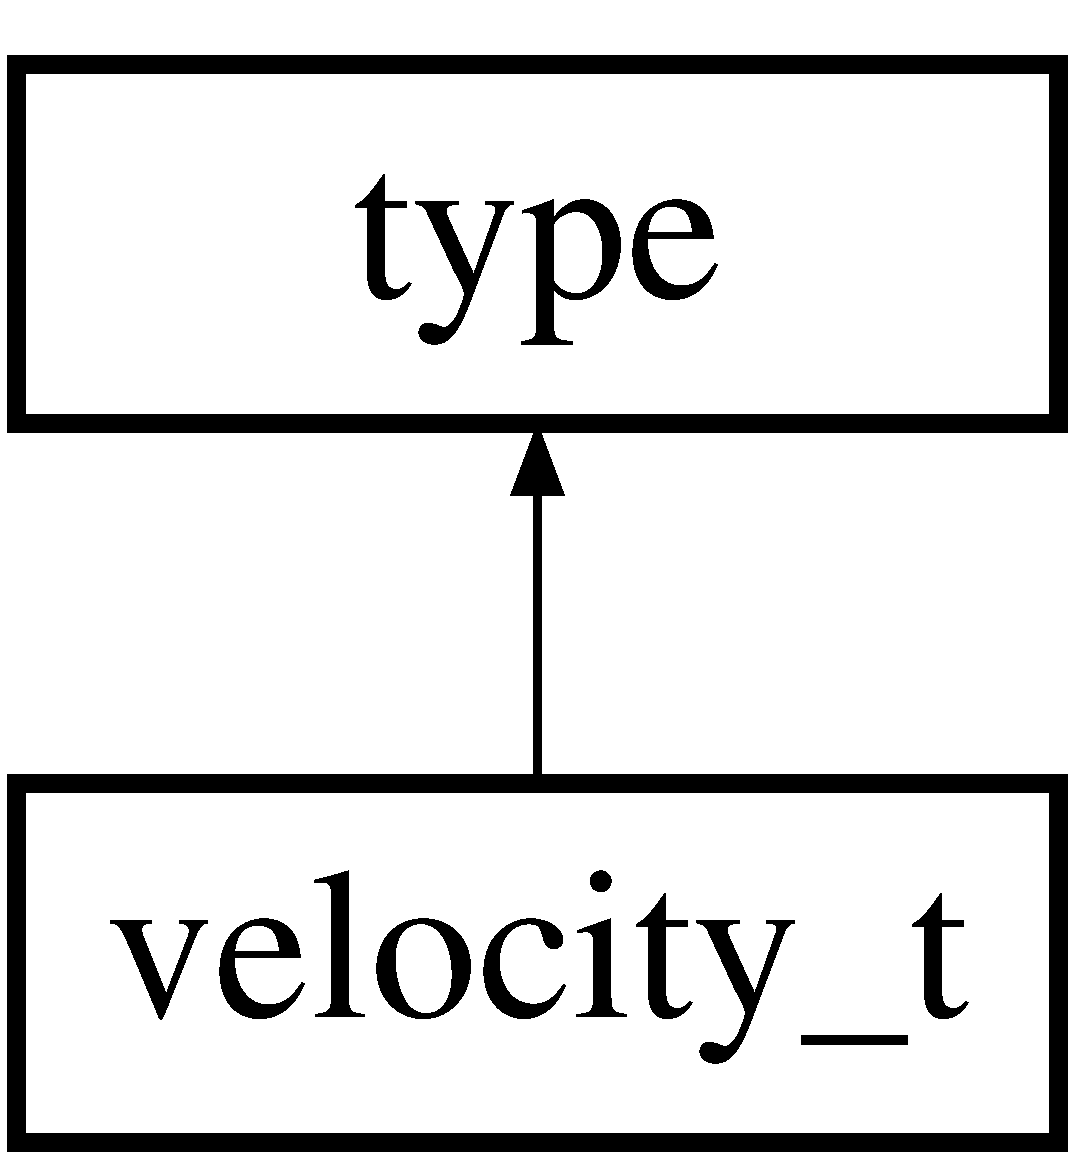
\includegraphics[height=2.000000cm]{classvelocity__t}
\end{center}
\end{figure}
\subsection*{Public Types}
\begin{DoxyCompactItemize}
\item 
typedef \-::\hyperlink{namespacexml__schema_a69bfaf24f63a8c18ebd8e21db6b343df}{xml\-\_\-schema\-::decimal} \hyperlink{classvelocity__t_a96ff8f29edf435cfe0966409d22b33c7}{x\-\_\-type}
\item 
typedef \\*
\-::xsd\-::cxx\-::tree\-::traits\\*
$<$ \hyperlink{classvelocity__t_a96ff8f29edf435cfe0966409d22b33c7}{x\-\_\-type}, char,\-::xsd\-::cxx\-::tree\-::schema\-\_\-type\-::decimal $>$ \hyperlink{classvelocity__t_a2fed2e212062cdd498a218d3c0ac8308}{x\-\_\-traits}
\item 
typedef \-::\hyperlink{namespacexml__schema_a69bfaf24f63a8c18ebd8e21db6b343df}{xml\-\_\-schema\-::decimal} \hyperlink{classvelocity__t_aab88921abbd89667cc4d293a448877f3}{y\-\_\-type}
\item 
typedef \\*
\-::xsd\-::cxx\-::tree\-::traits\\*
$<$ \hyperlink{classvelocity__t_aab88921abbd89667cc4d293a448877f3}{y\-\_\-type}, char,\-::xsd\-::cxx\-::tree\-::schema\-\_\-type\-::decimal $>$ \hyperlink{classvelocity__t_a315747a86c40ace5db31652413ae56a2}{y\-\_\-traits}
\item 
typedef \-::\hyperlink{namespacexml__schema_a69bfaf24f63a8c18ebd8e21db6b343df}{xml\-\_\-schema\-::decimal} \hyperlink{classvelocity__t_a0268003d7669eaa63abdcd4df2933316}{z\-\_\-type}
\item 
typedef \\*
\-::xsd\-::cxx\-::tree\-::traits\\*
$<$ \hyperlink{classvelocity__t_a0268003d7669eaa63abdcd4df2933316}{z\-\_\-type}, char,\-::xsd\-::cxx\-::tree\-::schema\-\_\-type\-::decimal $>$ \hyperlink{classvelocity__t_a7231515c9a7c3d2bbab96bccc8b12c6e}{z\-\_\-traits}
\end{DoxyCompactItemize}
\subsection*{Public Member Functions}
\begin{DoxyCompactItemize}
\item 
const \hyperlink{classvelocity__t_a96ff8f29edf435cfe0966409d22b33c7}{x\-\_\-type} \& \hyperlink{classvelocity__t_adc045e174c1631079cef733f987193c1}{x} () const 
\item 
\hyperlink{classvelocity__t_a96ff8f29edf435cfe0966409d22b33c7}{x\-\_\-type} \& \hyperlink{classvelocity__t_aeaea25c597e626199aa231e96df21c45}{x} ()
\item 
void \hyperlink{classvelocity__t_a51e6012bcd94ccde9169b8b38b8322bf}{x} (const \hyperlink{classvelocity__t_a96ff8f29edf435cfe0966409d22b33c7}{x\-\_\-type} \&x)
\item 
const \hyperlink{classvelocity__t_aab88921abbd89667cc4d293a448877f3}{y\-\_\-type} \& \hyperlink{classvelocity__t_a5470a18d9c20945aa0905b887fa5b19e}{y} () const 
\item 
\hyperlink{classvelocity__t_aab88921abbd89667cc4d293a448877f3}{y\-\_\-type} \& \hyperlink{classvelocity__t_a951fe39a3f18bc9057fd72ea45744914}{y} ()
\item 
void \hyperlink{classvelocity__t_a6f2874f8598611f2f3d2087cd2c6d33b}{y} (const \hyperlink{classvelocity__t_aab88921abbd89667cc4d293a448877f3}{y\-\_\-type} \&\hyperlink{classvelocity__t_adc045e174c1631079cef733f987193c1}{x})
\item 
const \hyperlink{classvelocity__t_a0268003d7669eaa63abdcd4df2933316}{z\-\_\-type} \& \hyperlink{classvelocity__t_a0ce6cb31c27de3b2e4f712a46ad40ce4}{z} () const 
\item 
\hyperlink{classvelocity__t_a0268003d7669eaa63abdcd4df2933316}{z\-\_\-type} \& \hyperlink{classvelocity__t_ae826294ca0cd396171920fad19a53c00}{z} ()
\item 
void \hyperlink{classvelocity__t_a6a25b6218ee7ca189fb6a6013b42502a}{z} (const \hyperlink{classvelocity__t_a0268003d7669eaa63abdcd4df2933316}{z\-\_\-type} \&\hyperlink{classvelocity__t_adc045e174c1631079cef733f987193c1}{x})
\item 
\hyperlink{classvelocity__t_acced6c7af3eca84743556a378e15b137}{velocity\-\_\-t} (const \hyperlink{classvelocity__t_a96ff8f29edf435cfe0966409d22b33c7}{x\-\_\-type} \&, const \hyperlink{classvelocity__t_aab88921abbd89667cc4d293a448877f3}{y\-\_\-type} \&, const \hyperlink{classvelocity__t_a0268003d7669eaa63abdcd4df2933316}{z\-\_\-type} \&)
\item 
\hyperlink{classvelocity__t_aac1f9f9123219851a0cf1bba38da4928}{velocity\-\_\-t} (const \-::xercesc\-::\-D\-O\-M\-Element \&e,\-::\hyperlink{namespacexml__schema_a0612287d030cb2732d31a45b258fdc87}{xml\-\_\-schema\-::flags} f=0,\-::\hyperlink{namespacexml__schema_ada9aa30dc722e93ee2ed7243085402a5}{xml\-\_\-schema\-::container} $\ast$c=0)
\item 
\hyperlink{classvelocity__t_ab0367cbbb5f78bb36bb7a6bb2eb1c965}{velocity\-\_\-t} (const \hyperlink{classvelocity__t}{velocity\-\_\-t} \&\hyperlink{classvelocity__t_adc045e174c1631079cef733f987193c1}{x},\-::\hyperlink{namespacexml__schema_a0612287d030cb2732d31a45b258fdc87}{xml\-\_\-schema\-::flags} f=0,\-::\hyperlink{namespacexml__schema_ada9aa30dc722e93ee2ed7243085402a5}{xml\-\_\-schema\-::container} $\ast$c=0)
\item 
virtual \hyperlink{classvelocity__t}{velocity\-\_\-t} $\ast$ \hyperlink{classvelocity__t_aaad3aac74b44916ce11b0312884a88ac}{\-\_\-clone} (\-::\hyperlink{namespacexml__schema_a0612287d030cb2732d31a45b258fdc87}{xml\-\_\-schema\-::flags} f=0,\-::\hyperlink{namespacexml__schema_ada9aa30dc722e93ee2ed7243085402a5}{xml\-\_\-schema\-::container} $\ast$c=0) const 
\item 
virtual \hyperlink{classvelocity__t_a5222577cd4e9f86f2cba6b44b8d416f8}{$\sim$velocity\-\_\-t} ()
\end{DoxyCompactItemize}
\subsection*{Protected Member Functions}
\begin{DoxyCompactItemize}
\item 
void \hyperlink{classvelocity__t_a815462c106c5ce40960f75cc331238e1}{parse} (\-::xsd\-::cxx\-::xml\-::dom\-::parser$<$ char $>$ \&,\-::\hyperlink{namespacexml__schema_a0612287d030cb2732d31a45b258fdc87}{xml\-\_\-schema\-::flags})
\end{DoxyCompactItemize}
\subsection*{Protected Attributes}
\begin{DoxyCompactItemize}
\item 
\-::xsd\-::cxx\-::tree\-::one$<$ \hyperlink{classvelocity__t_a96ff8f29edf435cfe0966409d22b33c7}{x\-\_\-type} $>$ \hyperlink{classvelocity__t_a648b432726339999caac51c3c72cb0de}{x\-\_\-}
\item 
\-::xsd\-::cxx\-::tree\-::one$<$ \hyperlink{classvelocity__t_aab88921abbd89667cc4d293a448877f3}{y\-\_\-type} $>$ \hyperlink{classvelocity__t_a6440f1e25ccd5916aff385482257ea71}{y\-\_\-}
\item 
\-::xsd\-::cxx\-::tree\-::one$<$ \hyperlink{classvelocity__t_a0268003d7669eaa63abdcd4df2933316}{z\-\_\-type} $>$ \hyperlink{classvelocity__t_a86e3de3b673d7c4f67aae4c3d866c17d}{z\-\_\-}
\end{DoxyCompactItemize}


\subsection{Member Typedef Documentation}
\hypertarget{classvelocity__t_a2fed2e212062cdd498a218d3c0ac8308}{\index{velocity\-\_\-t@{velocity\-\_\-t}!x\-\_\-traits@{x\-\_\-traits}}
\index{x\-\_\-traits@{x\-\_\-traits}!velocity_t@{velocity\-\_\-t}}
\subsubsection[{x\-\_\-traits}]{\setlength{\rightskip}{0pt plus 5cm}typedef \-::xsd\-::cxx\-::tree\-::traits$<$ {\bf x\-\_\-type}, char, \-::xsd\-::cxx\-::tree\-::schema\-\_\-type\-::decimal $>$ {\bf velocity\-\_\-t\-::x\-\_\-traits}}}\label{classvelocity__t_a2fed2e212062cdd498a218d3c0ac8308}
\hypertarget{classvelocity__t_a96ff8f29edf435cfe0966409d22b33c7}{\index{velocity\-\_\-t@{velocity\-\_\-t}!x\-\_\-type@{x\-\_\-type}}
\index{x\-\_\-type@{x\-\_\-type}!velocity_t@{velocity\-\_\-t}}
\subsubsection[{x\-\_\-type}]{\setlength{\rightskip}{0pt plus 5cm}typedef \-::{\bf xml\-\_\-schema\-::decimal} {\bf velocity\-\_\-t\-::x\-\_\-type}}}\label{classvelocity__t_a96ff8f29edf435cfe0966409d22b33c7}
\hypertarget{classvelocity__t_a315747a86c40ace5db31652413ae56a2}{\index{velocity\-\_\-t@{velocity\-\_\-t}!y\-\_\-traits@{y\-\_\-traits}}
\index{y\-\_\-traits@{y\-\_\-traits}!velocity_t@{velocity\-\_\-t}}
\subsubsection[{y\-\_\-traits}]{\setlength{\rightskip}{0pt plus 5cm}typedef \-::xsd\-::cxx\-::tree\-::traits$<$ {\bf y\-\_\-type}, char, \-::xsd\-::cxx\-::tree\-::schema\-\_\-type\-::decimal $>$ {\bf velocity\-\_\-t\-::y\-\_\-traits}}}\label{classvelocity__t_a315747a86c40ace5db31652413ae56a2}
\hypertarget{classvelocity__t_aab88921abbd89667cc4d293a448877f3}{\index{velocity\-\_\-t@{velocity\-\_\-t}!y\-\_\-type@{y\-\_\-type}}
\index{y\-\_\-type@{y\-\_\-type}!velocity_t@{velocity\-\_\-t}}
\subsubsection[{y\-\_\-type}]{\setlength{\rightskip}{0pt plus 5cm}typedef \-::{\bf xml\-\_\-schema\-::decimal} {\bf velocity\-\_\-t\-::y\-\_\-type}}}\label{classvelocity__t_aab88921abbd89667cc4d293a448877f3}
\hypertarget{classvelocity__t_a7231515c9a7c3d2bbab96bccc8b12c6e}{\index{velocity\-\_\-t@{velocity\-\_\-t}!z\-\_\-traits@{z\-\_\-traits}}
\index{z\-\_\-traits@{z\-\_\-traits}!velocity_t@{velocity\-\_\-t}}
\subsubsection[{z\-\_\-traits}]{\setlength{\rightskip}{0pt plus 5cm}typedef \-::xsd\-::cxx\-::tree\-::traits$<$ {\bf z\-\_\-type}, char, \-::xsd\-::cxx\-::tree\-::schema\-\_\-type\-::decimal $>$ {\bf velocity\-\_\-t\-::z\-\_\-traits}}}\label{classvelocity__t_a7231515c9a7c3d2bbab96bccc8b12c6e}
\hypertarget{classvelocity__t_a0268003d7669eaa63abdcd4df2933316}{\index{velocity\-\_\-t@{velocity\-\_\-t}!z\-\_\-type@{z\-\_\-type}}
\index{z\-\_\-type@{z\-\_\-type}!velocity_t@{velocity\-\_\-t}}
\subsubsection[{z\-\_\-type}]{\setlength{\rightskip}{0pt plus 5cm}typedef \-::{\bf xml\-\_\-schema\-::decimal} {\bf velocity\-\_\-t\-::z\-\_\-type}}}\label{classvelocity__t_a0268003d7669eaa63abdcd4df2933316}


\subsection{Constructor \& Destructor Documentation}
\hypertarget{classvelocity__t_acced6c7af3eca84743556a378e15b137}{\index{velocity\-\_\-t@{velocity\-\_\-t}!velocity\-\_\-t@{velocity\-\_\-t}}
\index{velocity\-\_\-t@{velocity\-\_\-t}!velocity_t@{velocity\-\_\-t}}
\subsubsection[{velocity\-\_\-t}]{\setlength{\rightskip}{0pt plus 5cm}velocity\-\_\-t\-::velocity\-\_\-t (
\begin{DoxyParamCaption}
\item[{const {\bf x\-\_\-type} \&}]{x, }
\item[{const {\bf y\-\_\-type} \&}]{y, }
\item[{const {\bf z\-\_\-type} \&}]{z}
\end{DoxyParamCaption}
)}}\label{classvelocity__t_acced6c7af3eca84743556a378e15b137}
\hypertarget{classvelocity__t_aac1f9f9123219851a0cf1bba38da4928}{\index{velocity\-\_\-t@{velocity\-\_\-t}!velocity\-\_\-t@{velocity\-\_\-t}}
\index{velocity\-\_\-t@{velocity\-\_\-t}!velocity_t@{velocity\-\_\-t}}
\subsubsection[{velocity\-\_\-t}]{\setlength{\rightskip}{0pt plus 5cm}velocity\-\_\-t\-::velocity\-\_\-t (
\begin{DoxyParamCaption}
\item[{const \-::xercesc\-::\-D\-O\-M\-Element \&}]{e, }
\item[{\-::{\bf xml\-\_\-schema\-::flags}}]{f = {\ttfamily 0}, }
\item[{\-::{\bf xml\-\_\-schema\-::container} $\ast$}]{c = {\ttfamily 0}}
\end{DoxyParamCaption}
)}}\label{classvelocity__t_aac1f9f9123219851a0cf1bba38da4928}
\hypertarget{classvelocity__t_ab0367cbbb5f78bb36bb7a6bb2eb1c965}{\index{velocity\-\_\-t@{velocity\-\_\-t}!velocity\-\_\-t@{velocity\-\_\-t}}
\index{velocity\-\_\-t@{velocity\-\_\-t}!velocity_t@{velocity\-\_\-t}}
\subsubsection[{velocity\-\_\-t}]{\setlength{\rightskip}{0pt plus 5cm}velocity\-\_\-t\-::velocity\-\_\-t (
\begin{DoxyParamCaption}
\item[{const {\bf velocity\-\_\-t} \&}]{x, }
\item[{\-::{\bf xml\-\_\-schema\-::flags}}]{f = {\ttfamily 0}, }
\item[{\-::{\bf xml\-\_\-schema\-::container} $\ast$}]{c = {\ttfamily 0}}
\end{DoxyParamCaption}
)}}\label{classvelocity__t_ab0367cbbb5f78bb36bb7a6bb2eb1c965}
\hypertarget{classvelocity__t_a5222577cd4e9f86f2cba6b44b8d416f8}{\index{velocity\-\_\-t@{velocity\-\_\-t}!$\sim$velocity\-\_\-t@{$\sim$velocity\-\_\-t}}
\index{$\sim$velocity\-\_\-t@{$\sim$velocity\-\_\-t}!velocity_t@{velocity\-\_\-t}}
\subsubsection[{$\sim$velocity\-\_\-t}]{\setlength{\rightskip}{0pt plus 5cm}velocity\-\_\-t\-::$\sim$velocity\-\_\-t (
\begin{DoxyParamCaption}
{}
\end{DoxyParamCaption}
)\hspace{0.3cm}{\ttfamily [virtual]}}}\label{classvelocity__t_a5222577cd4e9f86f2cba6b44b8d416f8}


\subsection{Member Function Documentation}
\hypertarget{classvelocity__t_aaad3aac74b44916ce11b0312884a88ac}{\index{velocity\-\_\-t@{velocity\-\_\-t}!\-\_\-clone@{\-\_\-clone}}
\index{\-\_\-clone@{\-\_\-clone}!velocity_t@{velocity\-\_\-t}}
\subsubsection[{\-\_\-clone}]{\setlength{\rightskip}{0pt plus 5cm}{\bf velocity\-\_\-t} $\ast$ velocity\-\_\-t\-::\-\_\-clone (
\begin{DoxyParamCaption}
\item[{\-::{\bf xml\-\_\-schema\-::flags}}]{f = {\ttfamily 0}, }
\item[{\-::{\bf xml\-\_\-schema\-::container} $\ast$}]{c = {\ttfamily 0}}
\end{DoxyParamCaption}
) const\hspace{0.3cm}{\ttfamily [virtual]}}}\label{classvelocity__t_aaad3aac74b44916ce11b0312884a88ac}
\hypertarget{classvelocity__t_a815462c106c5ce40960f75cc331238e1}{\index{velocity\-\_\-t@{velocity\-\_\-t}!parse@{parse}}
\index{parse@{parse}!velocity_t@{velocity\-\_\-t}}
\subsubsection[{parse}]{\setlength{\rightskip}{0pt plus 5cm}void velocity\-\_\-t\-::parse (
\begin{DoxyParamCaption}
\item[{\-::xsd\-::cxx\-::xml\-::dom\-::parser$<$ char $>$ \&}]{p, }
\item[{\-::{\bf xml\-\_\-schema\-::flags}}]{f}
\end{DoxyParamCaption}
)\hspace{0.3cm}{\ttfamily [protected]}}}\label{classvelocity__t_a815462c106c5ce40960f75cc331238e1}
\hypertarget{classvelocity__t_adc045e174c1631079cef733f987193c1}{\index{velocity\-\_\-t@{velocity\-\_\-t}!x@{x}}
\index{x@{x}!velocity_t@{velocity\-\_\-t}}
\subsubsection[{x}]{\setlength{\rightskip}{0pt plus 5cm}const {\bf velocity\-\_\-t\-::x\-\_\-type} \& velocity\-\_\-t\-::x (
\begin{DoxyParamCaption}
{}
\end{DoxyParamCaption}
) const}}\label{classvelocity__t_adc045e174c1631079cef733f987193c1}
\hypertarget{classvelocity__t_aeaea25c597e626199aa231e96df21c45}{\index{velocity\-\_\-t@{velocity\-\_\-t}!x@{x}}
\index{x@{x}!velocity_t@{velocity\-\_\-t}}
\subsubsection[{x}]{\setlength{\rightskip}{0pt plus 5cm}{\bf velocity\-\_\-t\-::x\-\_\-type} \& velocity\-\_\-t\-::x (
\begin{DoxyParamCaption}
{}
\end{DoxyParamCaption}
)}}\label{classvelocity__t_aeaea25c597e626199aa231e96df21c45}
\hypertarget{classvelocity__t_a51e6012bcd94ccde9169b8b38b8322bf}{\index{velocity\-\_\-t@{velocity\-\_\-t}!x@{x}}
\index{x@{x}!velocity_t@{velocity\-\_\-t}}
\subsubsection[{x}]{\setlength{\rightskip}{0pt plus 5cm}void velocity\-\_\-t\-::x (
\begin{DoxyParamCaption}
\item[{const {\bf x\-\_\-type} \&}]{x}
\end{DoxyParamCaption}
)}}\label{classvelocity__t_a51e6012bcd94ccde9169b8b38b8322bf}
\hypertarget{classvelocity__t_a5470a18d9c20945aa0905b887fa5b19e}{\index{velocity\-\_\-t@{velocity\-\_\-t}!y@{y}}
\index{y@{y}!velocity_t@{velocity\-\_\-t}}
\subsubsection[{y}]{\setlength{\rightskip}{0pt plus 5cm}const {\bf velocity\-\_\-t\-::y\-\_\-type} \& velocity\-\_\-t\-::y (
\begin{DoxyParamCaption}
{}
\end{DoxyParamCaption}
) const}}\label{classvelocity__t_a5470a18d9c20945aa0905b887fa5b19e}
\hypertarget{classvelocity__t_a951fe39a3f18bc9057fd72ea45744914}{\index{velocity\-\_\-t@{velocity\-\_\-t}!y@{y}}
\index{y@{y}!velocity_t@{velocity\-\_\-t}}
\subsubsection[{y}]{\setlength{\rightskip}{0pt plus 5cm}{\bf velocity\-\_\-t\-::y\-\_\-type} \& velocity\-\_\-t\-::y (
\begin{DoxyParamCaption}
{}
\end{DoxyParamCaption}
)}}\label{classvelocity__t_a951fe39a3f18bc9057fd72ea45744914}
\hypertarget{classvelocity__t_a6f2874f8598611f2f3d2087cd2c6d33b}{\index{velocity\-\_\-t@{velocity\-\_\-t}!y@{y}}
\index{y@{y}!velocity_t@{velocity\-\_\-t}}
\subsubsection[{y}]{\setlength{\rightskip}{0pt plus 5cm}void velocity\-\_\-t\-::y (
\begin{DoxyParamCaption}
\item[{const {\bf y\-\_\-type} \&}]{x}
\end{DoxyParamCaption}
)}}\label{classvelocity__t_a6f2874f8598611f2f3d2087cd2c6d33b}
\hypertarget{classvelocity__t_a0ce6cb31c27de3b2e4f712a46ad40ce4}{\index{velocity\-\_\-t@{velocity\-\_\-t}!z@{z}}
\index{z@{z}!velocity_t@{velocity\-\_\-t}}
\subsubsection[{z}]{\setlength{\rightskip}{0pt plus 5cm}const {\bf velocity\-\_\-t\-::z\-\_\-type} \& velocity\-\_\-t\-::z (
\begin{DoxyParamCaption}
{}
\end{DoxyParamCaption}
) const}}\label{classvelocity__t_a0ce6cb31c27de3b2e4f712a46ad40ce4}
\hypertarget{classvelocity__t_ae826294ca0cd396171920fad19a53c00}{\index{velocity\-\_\-t@{velocity\-\_\-t}!z@{z}}
\index{z@{z}!velocity_t@{velocity\-\_\-t}}
\subsubsection[{z}]{\setlength{\rightskip}{0pt plus 5cm}{\bf velocity\-\_\-t\-::z\-\_\-type} \& velocity\-\_\-t\-::z (
\begin{DoxyParamCaption}
{}
\end{DoxyParamCaption}
)}}\label{classvelocity__t_ae826294ca0cd396171920fad19a53c00}
\hypertarget{classvelocity__t_a6a25b6218ee7ca189fb6a6013b42502a}{\index{velocity\-\_\-t@{velocity\-\_\-t}!z@{z}}
\index{z@{z}!velocity_t@{velocity\-\_\-t}}
\subsubsection[{z}]{\setlength{\rightskip}{0pt plus 5cm}void velocity\-\_\-t\-::z (
\begin{DoxyParamCaption}
\item[{const {\bf z\-\_\-type} \&}]{x}
\end{DoxyParamCaption}
)}}\label{classvelocity__t_a6a25b6218ee7ca189fb6a6013b42502a}


\subsection{Member Data Documentation}
\hypertarget{classvelocity__t_a648b432726339999caac51c3c72cb0de}{\index{velocity\-\_\-t@{velocity\-\_\-t}!x\-\_\-@{x\-\_\-}}
\index{x\-\_\-@{x\-\_\-}!velocity_t@{velocity\-\_\-t}}
\subsubsection[{x\-\_\-}]{\setlength{\rightskip}{0pt plus 5cm}\-::xsd\-::cxx\-::tree\-::one$<$ {\bf x\-\_\-type} $>$ velocity\-\_\-t\-::x\-\_\-\hspace{0.3cm}{\ttfamily [protected]}}}\label{classvelocity__t_a648b432726339999caac51c3c72cb0de}
\hypertarget{classvelocity__t_a6440f1e25ccd5916aff385482257ea71}{\index{velocity\-\_\-t@{velocity\-\_\-t}!y\-\_\-@{y\-\_\-}}
\index{y\-\_\-@{y\-\_\-}!velocity_t@{velocity\-\_\-t}}
\subsubsection[{y\-\_\-}]{\setlength{\rightskip}{0pt plus 5cm}\-::xsd\-::cxx\-::tree\-::one$<$ {\bf y\-\_\-type} $>$ velocity\-\_\-t\-::y\-\_\-\hspace{0.3cm}{\ttfamily [protected]}}}\label{classvelocity__t_a6440f1e25ccd5916aff385482257ea71}
\hypertarget{classvelocity__t_a86e3de3b673d7c4f67aae4c3d866c17d}{\index{velocity\-\_\-t@{velocity\-\_\-t}!z\-\_\-@{z\-\_\-}}
\index{z\-\_\-@{z\-\_\-}!velocity_t@{velocity\-\_\-t}}
\subsubsection[{z\-\_\-}]{\setlength{\rightskip}{0pt plus 5cm}\-::xsd\-::cxx\-::tree\-::one$<$ {\bf z\-\_\-type} $>$ velocity\-\_\-t\-::z\-\_\-\hspace{0.3cm}{\ttfamily [protected]}}}\label{classvelocity__t_a86e3de3b673d7c4f67aae4c3d866c17d}


The documentation for this class was generated from the following files\-:\begin{DoxyCompactItemize}
\item 
src/utils/\hyperlink{InputParticles_8h}{Input\-Particles.\-h}\item 
src/utils/\hyperlink{InputParticles_8cpp}{Input\-Particles.\-cpp}\end{DoxyCompactItemize}

\hypertarget{classVTKFile__t}{\section{V\-T\-K\-File\-\_\-t Class Reference}
\label{classVTKFile__t}\index{V\-T\-K\-File\-\_\-t@{V\-T\-K\-File\-\_\-t}}
}


Class corresponding to the V\-T\-K\-File\-\_\-t schema type.  




{\ttfamily \#include $<$vtk-\/unstructured.\-h$>$}

Inheritance diagram for V\-T\-K\-File\-\_\-t\-:\begin{figure}[H]
\begin{center}
\leavevmode
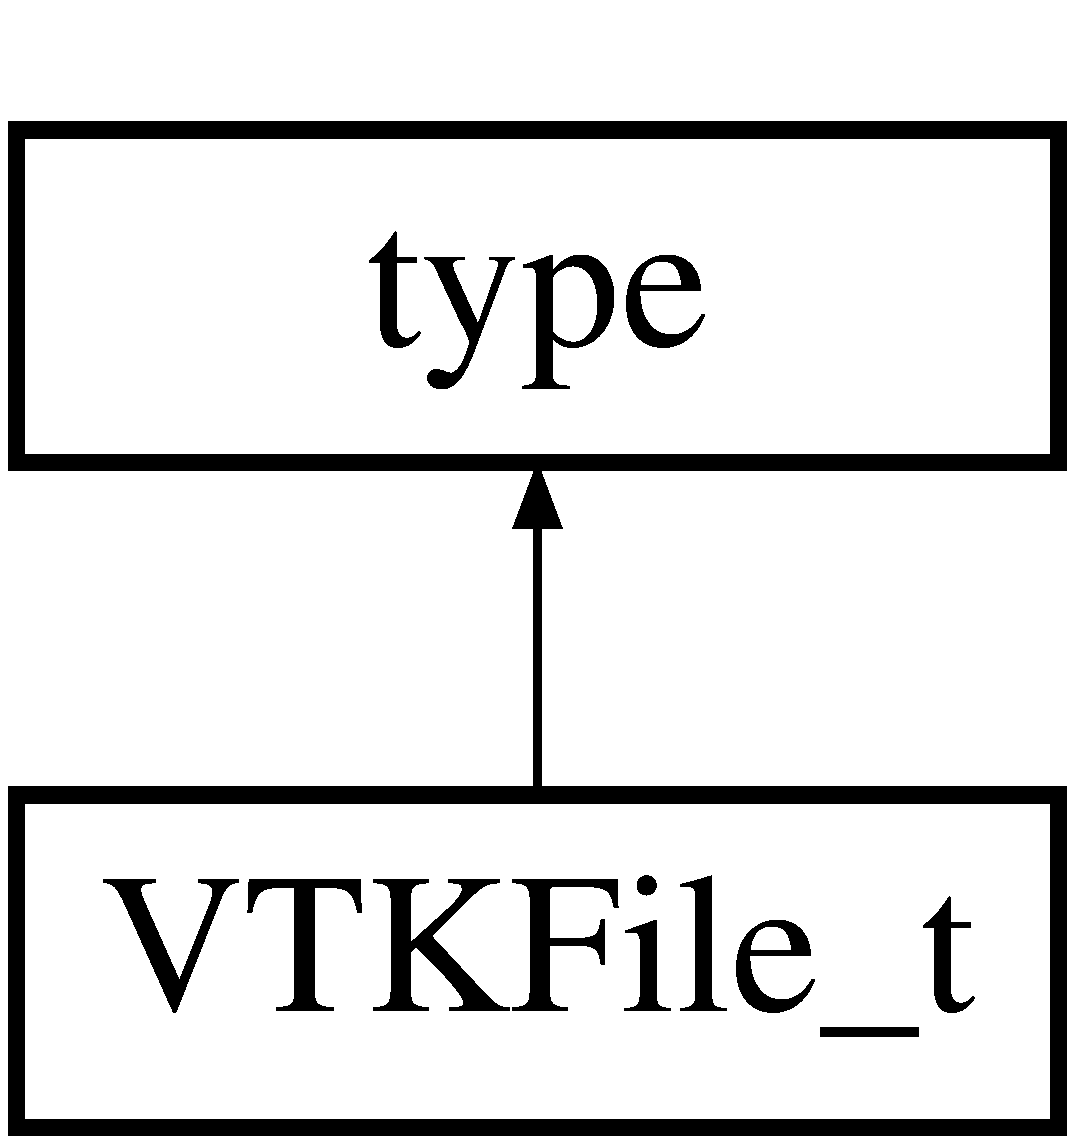
\includegraphics[height=2.000000cm]{classVTKFile__t}
\end{center}
\end{figure}
\subsection*{Public Member Functions}
\begin{DoxyCompactItemize}
\item 
virtual \hyperlink{classVTKFile__t_ac5cf95c81660088dbb3c9ab6cd78dede}{$\sim$\-V\-T\-K\-File\-\_\-t} ()
\begin{DoxyCompactList}\small\item\em Destructor. \end{DoxyCompactList}\end{DoxyCompactItemize}
\subsection*{Unstructured\-Grid}
\label{_amgrp51267337395fceec37fec7e87b9a53e5}%
Accessor and modifier functions for the Unstructured\-Grid optional element. \begin{DoxyCompactItemize}
\item 
typedef \-::\hyperlink{classUnstructuredGrid__t}{Unstructured\-Grid\-\_\-t} \hyperlink{classVTKFile__t_a34ea02f6804e701657f11a8dc3851951}{Unstructured\-Grid\-\_\-type}
\begin{DoxyCompactList}\small\item\em Element type. \end{DoxyCompactList}\item 
typedef \\*
\-::xsd\-::cxx\-::tree\-::optional\\*
$<$ \hyperlink{classVTKFile__t_a34ea02f6804e701657f11a8dc3851951}{Unstructured\-Grid\-\_\-type} $>$ \hyperlink{classVTKFile__t_ada5bb5a706e03ef1ab2ed1513ea83833}{Unstructured\-Grid\-\_\-optional}
\begin{DoxyCompactList}\small\item\em Element optional container type. \end{DoxyCompactList}\item 
typedef \\*
\-::xsd\-::cxx\-::tree\-::traits\\*
$<$ \hyperlink{classVTKFile__t_a34ea02f6804e701657f11a8dc3851951}{Unstructured\-Grid\-\_\-type}, char $>$ \hyperlink{classVTKFile__t_a02772a5f713678f02e94188d6a552528}{Unstructured\-Grid\-\_\-traits}
\begin{DoxyCompactList}\small\item\em Element traits type. \end{DoxyCompactList}\item 
const \hyperlink{classVTKFile__t_ada5bb5a706e03ef1ab2ed1513ea83833}{Unstructured\-Grid\-\_\-optional} \& \hyperlink{classVTKFile__t_a118852d8ec1f8039d1fd5c914282351a}{Unstructured\-Grid} () const 
\begin{DoxyCompactList}\small\item\em Return a read-\/only (constant) reference to the element container. \end{DoxyCompactList}\item 
\hyperlink{classVTKFile__t_ada5bb5a706e03ef1ab2ed1513ea83833}{Unstructured\-Grid\-\_\-optional} \& \hyperlink{classVTKFile__t_aa4746d4a723076d4643b8ef16a9c3890}{Unstructured\-Grid} ()
\begin{DoxyCompactList}\small\item\em Return a read-\/write reference to the element container. \end{DoxyCompactList}\item 
void \hyperlink{classVTKFile__t_a2c2b1b2ff487c7e61bcd2875db8747be}{Unstructured\-Grid} (const \hyperlink{classVTKFile__t_a34ea02f6804e701657f11a8dc3851951}{Unstructured\-Grid\-\_\-type} \&x)
\begin{DoxyCompactList}\small\item\em Set the element value. \end{DoxyCompactList}\item 
void \hyperlink{classVTKFile__t_ae33d9781bddb747f9255570b1af2dfeb}{Unstructured\-Grid} (const \hyperlink{classVTKFile__t_ada5bb5a706e03ef1ab2ed1513ea83833}{Unstructured\-Grid\-\_\-optional} \&x)
\begin{DoxyCompactList}\small\item\em Set the element value. \end{DoxyCompactList}\item 
void \hyperlink{classVTKFile__t_af19a966f55acb5f03299af922bd9dd75}{Unstructured\-Grid} (\-::std\-::auto\-\_\-ptr$<$ \hyperlink{classVTKFile__t_a34ea02f6804e701657f11a8dc3851951}{Unstructured\-Grid\-\_\-type} $>$ p)
\begin{DoxyCompactList}\small\item\em Set the element value without copying. \end{DoxyCompactList}\end{DoxyCompactItemize}
\subsection*{Poly\-Data}
\label{_amgrpf4abb74983d657d0185d4dd07cff9b2c}%
Accessor and modifier functions for the Poly\-Data optional element. \begin{DoxyCompactItemize}
\item 
typedef \-::\hyperlink{classPolyData__t}{Poly\-Data\-\_\-t} \hyperlink{classVTKFile__t_a4588b4f0e28ba09aa219bda7e1fc6c97}{Poly\-Data\-\_\-type}
\begin{DoxyCompactList}\small\item\em Element type. \end{DoxyCompactList}\item 
typedef \\*
\-::xsd\-::cxx\-::tree\-::optional\\*
$<$ \hyperlink{classVTKFile__t_a4588b4f0e28ba09aa219bda7e1fc6c97}{Poly\-Data\-\_\-type} $>$ \hyperlink{classVTKFile__t_aacb796775ae228cd61726a23b809f3e4}{Poly\-Data\-\_\-optional}
\begin{DoxyCompactList}\small\item\em Element optional container type. \end{DoxyCompactList}\item 
typedef \\*
\-::xsd\-::cxx\-::tree\-::traits\\*
$<$ \hyperlink{classVTKFile__t_a4588b4f0e28ba09aa219bda7e1fc6c97}{Poly\-Data\-\_\-type}, char $>$ \hyperlink{classVTKFile__t_aa5ad98f5709c1e9beec3804a7f42b5f6}{Poly\-Data\-\_\-traits}
\begin{DoxyCompactList}\small\item\em Element traits type. \end{DoxyCompactList}\item 
const \hyperlink{classVTKFile__t_aacb796775ae228cd61726a23b809f3e4}{Poly\-Data\-\_\-optional} \& \hyperlink{classVTKFile__t_a7d728d7f31157fc80117c2f80978344c}{Poly\-Data} () const 
\begin{DoxyCompactList}\small\item\em Return a read-\/only (constant) reference to the element container. \end{DoxyCompactList}\item 
\hyperlink{classVTKFile__t_aacb796775ae228cd61726a23b809f3e4}{Poly\-Data\-\_\-optional} \& \hyperlink{classVTKFile__t_a0f87118c1898bc43619fa0bade52e921}{Poly\-Data} ()
\begin{DoxyCompactList}\small\item\em Return a read-\/write reference to the element container. \end{DoxyCompactList}\item 
void \hyperlink{classVTKFile__t_ab0a3f2aa2894d0384a89a6e5490c9372}{Poly\-Data} (const \hyperlink{classVTKFile__t_a4588b4f0e28ba09aa219bda7e1fc6c97}{Poly\-Data\-\_\-type} \&x)
\begin{DoxyCompactList}\small\item\em Set the element value. \end{DoxyCompactList}\item 
void \hyperlink{classVTKFile__t_a1c2a800d41431c04965c863220a3b1b5}{Poly\-Data} (const \hyperlink{classVTKFile__t_aacb796775ae228cd61726a23b809f3e4}{Poly\-Data\-\_\-optional} \&x)
\begin{DoxyCompactList}\small\item\em Set the element value. \end{DoxyCompactList}\item 
void \hyperlink{classVTKFile__t_a8ae292e04bf2c955d8f50cdeb60f9369}{Poly\-Data} (\-::std\-::auto\-\_\-ptr$<$ \hyperlink{classVTKFile__t_a4588b4f0e28ba09aa219bda7e1fc6c97}{Poly\-Data\-\_\-type} $>$ p)
\begin{DoxyCompactList}\small\item\em Set the element value without copying. \end{DoxyCompactList}\end{DoxyCompactItemize}
\subsection*{type}
\label{_amgrp599dcce2998a6b40b1e38e8c6006cb0a}%
Accessor and modifier functions for the type required attribute. \begin{DoxyCompactItemize}
\item 
typedef \-::\hyperlink{namespacexml__schema_ac0cec83a330f0024e4e318b3deac5104}{xml\-\_\-schema\-::string} \hyperlink{classVTKFile__t_ac1f3484e4fde414849ede43a00955f76}{type\-\_\-type}
\begin{DoxyCompactList}\small\item\em Attribute type. \end{DoxyCompactList}\item 
typedef \\*
\-::xsd\-::cxx\-::tree\-::traits\\*
$<$ \hyperlink{classVTKFile__t_ac1f3484e4fde414849ede43a00955f76}{type\-\_\-type}, char $>$ \hyperlink{classVTKFile__t_aee4ac167e843e9def1be4f43ad930391}{type\-\_\-traits}
\begin{DoxyCompactList}\small\item\em Attribute traits type. \end{DoxyCompactList}\item 
const \hyperlink{classVTKFile__t_ac1f3484e4fde414849ede43a00955f76}{type\-\_\-type} \& \hyperlink{classVTKFile__t_a5c23301c79cc6a376fe2abce533b2cf7}{type} () const 
\begin{DoxyCompactList}\small\item\em Return a read-\/only (constant) reference to the attribute. \end{DoxyCompactList}\item 
\hyperlink{classVTKFile__t_ac1f3484e4fde414849ede43a00955f76}{type\-\_\-type} \& \hyperlink{classVTKFile__t_abcc8ab822fa4f9e5e5294f5d8cff05c2}{type} ()
\begin{DoxyCompactList}\small\item\em Return a read-\/write reference to the attribute. \end{DoxyCompactList}\item 
void \hyperlink{classVTKFile__t_a6423eb2dc7fa367417df87de4921301e}{type} (const \hyperlink{classVTKFile__t_ac1f3484e4fde414849ede43a00955f76}{type\-\_\-type} \&x)
\begin{DoxyCompactList}\small\item\em Set the attribute value. \end{DoxyCompactList}\item 
void \hyperlink{classVTKFile__t_a380c8628fd1095c88a80a1804837c213}{type} (\-::std\-::auto\-\_\-ptr$<$ \hyperlink{classVTKFile__t_ac1f3484e4fde414849ede43a00955f76}{type\-\_\-type} $>$ p)
\begin{DoxyCompactList}\small\item\em Set the attribute value without copying. \end{DoxyCompactList}\end{DoxyCompactItemize}
\subsection*{version}
\label{_amgrp2af72f100c356273d46284f6fd1dfc08}%
Accessor and modifier functions for the version required attribute. \begin{DoxyCompactItemize}
\item 
typedef \-::\hyperlink{namespacexml__schema_ac0cec83a330f0024e4e318b3deac5104}{xml\-\_\-schema\-::string} \hyperlink{classVTKFile__t_a7db6f6d11f363380d6361446f5dede7b}{version\-\_\-type}
\begin{DoxyCompactList}\small\item\em Attribute type. \end{DoxyCompactList}\item 
typedef \\*
\-::xsd\-::cxx\-::tree\-::traits\\*
$<$ \hyperlink{classVTKFile__t_a7db6f6d11f363380d6361446f5dede7b}{version\-\_\-type}, char $>$ \hyperlink{classVTKFile__t_a5a343e08417564e5db3f48859b1a0c5f}{version\-\_\-traits}
\begin{DoxyCompactList}\small\item\em Attribute traits type. \end{DoxyCompactList}\item 
const \hyperlink{classVTKFile__t_a7db6f6d11f363380d6361446f5dede7b}{version\-\_\-type} \& \hyperlink{classVTKFile__t_af0f1ed9d44019ad1fab6495b6ae71a47}{version} () const 
\begin{DoxyCompactList}\small\item\em Return a read-\/only (constant) reference to the attribute. \end{DoxyCompactList}\item 
static const \hyperlink{classVTKFile__t_a7db6f6d11f363380d6361446f5dede7b}{version\-\_\-type} \& \hyperlink{classVTKFile__t_a0eb5afa9ec6125c0519a891578f31521}{version\-\_\-default\-\_\-value} ()
\begin{DoxyCompactList}\small\item\em Return the default value for the attribute. \end{DoxyCompactList}\end{DoxyCompactItemize}
\subsection*{byte\-\_\-order}
\label{_amgrp4d85380f9aa2c7bfea4b497dbb3373af}%
Accessor and modifier functions for the byte\-\_\-order required attribute. \begin{DoxyCompactItemize}
\item 
typedef \-::\hyperlink{namespacexml__schema_ac0cec83a330f0024e4e318b3deac5104}{xml\-\_\-schema\-::string} \hyperlink{classVTKFile__t_ab08dd45c560dd0635d0e5c0a5e42d2e8}{byte\-\_\-order\-\_\-type}
\begin{DoxyCompactList}\small\item\em Attribute type. \end{DoxyCompactList}\item 
typedef \\*
\-::xsd\-::cxx\-::tree\-::traits\\*
$<$ \hyperlink{classVTKFile__t_ab08dd45c560dd0635d0e5c0a5e42d2e8}{byte\-\_\-order\-\_\-type}, char $>$ \hyperlink{classVTKFile__t_ae0b8c254bc373d9218ea9eab406b7b98}{byte\-\_\-order\-\_\-traits}
\begin{DoxyCompactList}\small\item\em Attribute traits type. \end{DoxyCompactList}\item 
const \hyperlink{classVTKFile__t_ab08dd45c560dd0635d0e5c0a5e42d2e8}{byte\-\_\-order\-\_\-type} \& \hyperlink{classVTKFile__t_ad87b4f45ca18139b1ffae8ce08dc2e27}{byte\-\_\-order} () const 
\begin{DoxyCompactList}\small\item\em Return a read-\/only (constant) reference to the attribute. \end{DoxyCompactList}\item 
static const \hyperlink{classVTKFile__t_ab08dd45c560dd0635d0e5c0a5e42d2e8}{byte\-\_\-order\-\_\-type} \& \hyperlink{classVTKFile__t_a4538fe428d79eff40025d874e200bec1}{byte\-\_\-order\-\_\-default\-\_\-value} ()
\begin{DoxyCompactList}\small\item\em Return the default value for the attribute. \end{DoxyCompactList}\end{DoxyCompactItemize}
\subsection*{Constructors}
\begin{DoxyCompactItemize}
\item 
\hyperlink{classVTKFile__t_a76547340cb91ad0019d45889ca69fda0}{V\-T\-K\-File\-\_\-t} (const \hyperlink{classVTKFile__t_ac1f3484e4fde414849ede43a00955f76}{type\-\_\-type} \&)
\begin{DoxyCompactList}\small\item\em Create an instance from the ultimate base and initializers for required elements and attributes. \end{DoxyCompactList}\item 
\hyperlink{classVTKFile__t_a5d1c8c263c9865fe6f4b6ae1446efcaf}{V\-T\-K\-File\-\_\-t} (const \-::xercesc\-::\-D\-O\-M\-Element \&e,\-::\hyperlink{namespacexml__schema_a0612287d030cb2732d31a45b258fdc87}{xml\-\_\-schema\-::flags} f=0,\-::\hyperlink{namespacexml__schema_ada9aa30dc722e93ee2ed7243085402a5}{xml\-\_\-schema\-::container} $\ast$c=0)
\begin{DoxyCompactList}\small\item\em Create an instance from a D\-O\-M element. \end{DoxyCompactList}\item 
\hyperlink{classVTKFile__t_af239970202f0aee8392cb0af61863f62}{V\-T\-K\-File\-\_\-t} (const \hyperlink{classVTKFile__t}{V\-T\-K\-File\-\_\-t} \&x,\-::\hyperlink{namespacexml__schema_a0612287d030cb2732d31a45b258fdc87}{xml\-\_\-schema\-::flags} f=0,\-::\hyperlink{namespacexml__schema_ada9aa30dc722e93ee2ed7243085402a5}{xml\-\_\-schema\-::container} $\ast$c=0)
\begin{DoxyCompactList}\small\item\em Copy constructor. \end{DoxyCompactList}\item 
virtual \hyperlink{classVTKFile__t}{V\-T\-K\-File\-\_\-t} $\ast$ \hyperlink{classVTKFile__t_ad39ce94f7390685f9717fd521bac36e3}{\-\_\-clone} (\-::\hyperlink{namespacexml__schema_a0612287d030cb2732d31a45b258fdc87}{xml\-\_\-schema\-::flags} f=0,\-::\hyperlink{namespacexml__schema_ada9aa30dc722e93ee2ed7243085402a5}{xml\-\_\-schema\-::container} $\ast$c=0) const 
\begin{DoxyCompactList}\small\item\em Copy the instance polymorphically. \end{DoxyCompactList}\end{DoxyCompactItemize}


\subsection{Detailed Description}
Class corresponding to the V\-T\-K\-File\-\_\-t schema type. 

The hello\-\_\-t type consists of a greeting phrase and a collection of names to which this greeting applies. 

\subsection{Member Typedef Documentation}
\hypertarget{classVTKFile__t_ae0b8c254bc373d9218ea9eab406b7b98}{\index{V\-T\-K\-File\-\_\-t@{V\-T\-K\-File\-\_\-t}!byte\-\_\-order\-\_\-traits@{byte\-\_\-order\-\_\-traits}}
\index{byte\-\_\-order\-\_\-traits@{byte\-\_\-order\-\_\-traits}!VTKFile_t@{V\-T\-K\-File\-\_\-t}}
\subsubsection[{byte\-\_\-order\-\_\-traits}]{\setlength{\rightskip}{0pt plus 5cm}typedef \-::xsd\-::cxx\-::tree\-::traits$<$ {\bf byte\-\_\-order\-\_\-type}, char $>$ {\bf V\-T\-K\-File\-\_\-t\-::byte\-\_\-order\-\_\-traits}}}\label{classVTKFile__t_ae0b8c254bc373d9218ea9eab406b7b98}


Attribute traits type. 

\hypertarget{classVTKFile__t_ab08dd45c560dd0635d0e5c0a5e42d2e8}{\index{V\-T\-K\-File\-\_\-t@{V\-T\-K\-File\-\_\-t}!byte\-\_\-order\-\_\-type@{byte\-\_\-order\-\_\-type}}
\index{byte\-\_\-order\-\_\-type@{byte\-\_\-order\-\_\-type}!VTKFile_t@{V\-T\-K\-File\-\_\-t}}
\subsubsection[{byte\-\_\-order\-\_\-type}]{\setlength{\rightskip}{0pt plus 5cm}typedef \-::{\bf xml\-\_\-schema\-::string} {\bf V\-T\-K\-File\-\_\-t\-::byte\-\_\-order\-\_\-type}}}\label{classVTKFile__t_ab08dd45c560dd0635d0e5c0a5e42d2e8}


Attribute type. 

\hypertarget{classVTKFile__t_aacb796775ae228cd61726a23b809f3e4}{\index{V\-T\-K\-File\-\_\-t@{V\-T\-K\-File\-\_\-t}!Poly\-Data\-\_\-optional@{Poly\-Data\-\_\-optional}}
\index{Poly\-Data\-\_\-optional@{Poly\-Data\-\_\-optional}!VTKFile_t@{V\-T\-K\-File\-\_\-t}}
\subsubsection[{Poly\-Data\-\_\-optional}]{\setlength{\rightskip}{0pt plus 5cm}typedef \-::xsd\-::cxx\-::tree\-::optional$<$ {\bf Poly\-Data\-\_\-type} $>$ {\bf V\-T\-K\-File\-\_\-t\-::\-Poly\-Data\-\_\-optional}}}\label{classVTKFile__t_aacb796775ae228cd61726a23b809f3e4}


Element optional container type. 

\hypertarget{classVTKFile__t_aa5ad98f5709c1e9beec3804a7f42b5f6}{\index{V\-T\-K\-File\-\_\-t@{V\-T\-K\-File\-\_\-t}!Poly\-Data\-\_\-traits@{Poly\-Data\-\_\-traits}}
\index{Poly\-Data\-\_\-traits@{Poly\-Data\-\_\-traits}!VTKFile_t@{V\-T\-K\-File\-\_\-t}}
\subsubsection[{Poly\-Data\-\_\-traits}]{\setlength{\rightskip}{0pt plus 5cm}typedef \-::xsd\-::cxx\-::tree\-::traits$<$ {\bf Poly\-Data\-\_\-type}, char $>$ {\bf V\-T\-K\-File\-\_\-t\-::\-Poly\-Data\-\_\-traits}}}\label{classVTKFile__t_aa5ad98f5709c1e9beec3804a7f42b5f6}


Element traits type. 

\hypertarget{classVTKFile__t_a4588b4f0e28ba09aa219bda7e1fc6c97}{\index{V\-T\-K\-File\-\_\-t@{V\-T\-K\-File\-\_\-t}!Poly\-Data\-\_\-type@{Poly\-Data\-\_\-type}}
\index{Poly\-Data\-\_\-type@{Poly\-Data\-\_\-type}!VTKFile_t@{V\-T\-K\-File\-\_\-t}}
\subsubsection[{Poly\-Data\-\_\-type}]{\setlength{\rightskip}{0pt plus 5cm}typedef \-::{\bf Poly\-Data\-\_\-t} {\bf V\-T\-K\-File\-\_\-t\-::\-Poly\-Data\-\_\-type}}}\label{classVTKFile__t_a4588b4f0e28ba09aa219bda7e1fc6c97}


Element type. 

\hypertarget{classVTKFile__t_aee4ac167e843e9def1be4f43ad930391}{\index{V\-T\-K\-File\-\_\-t@{V\-T\-K\-File\-\_\-t}!type\-\_\-traits@{type\-\_\-traits}}
\index{type\-\_\-traits@{type\-\_\-traits}!VTKFile_t@{V\-T\-K\-File\-\_\-t}}
\subsubsection[{type\-\_\-traits}]{\setlength{\rightskip}{0pt plus 5cm}typedef \-::xsd\-::cxx\-::tree\-::traits$<$ {\bf type\-\_\-type}, char $>$ {\bf V\-T\-K\-File\-\_\-t\-::type\-\_\-traits}}}\label{classVTKFile__t_aee4ac167e843e9def1be4f43ad930391}


Attribute traits type. 

\hypertarget{classVTKFile__t_ac1f3484e4fde414849ede43a00955f76}{\index{V\-T\-K\-File\-\_\-t@{V\-T\-K\-File\-\_\-t}!type\-\_\-type@{type\-\_\-type}}
\index{type\-\_\-type@{type\-\_\-type}!VTKFile_t@{V\-T\-K\-File\-\_\-t}}
\subsubsection[{type\-\_\-type}]{\setlength{\rightskip}{0pt plus 5cm}typedef \-::{\bf xml\-\_\-schema\-::string} {\bf V\-T\-K\-File\-\_\-t\-::type\-\_\-type}}}\label{classVTKFile__t_ac1f3484e4fde414849ede43a00955f76}


Attribute type. 

\hypertarget{classVTKFile__t_ada5bb5a706e03ef1ab2ed1513ea83833}{\index{V\-T\-K\-File\-\_\-t@{V\-T\-K\-File\-\_\-t}!Unstructured\-Grid\-\_\-optional@{Unstructured\-Grid\-\_\-optional}}
\index{Unstructured\-Grid\-\_\-optional@{Unstructured\-Grid\-\_\-optional}!VTKFile_t@{V\-T\-K\-File\-\_\-t}}
\subsubsection[{Unstructured\-Grid\-\_\-optional}]{\setlength{\rightskip}{0pt plus 5cm}typedef \-::xsd\-::cxx\-::tree\-::optional$<$ {\bf Unstructured\-Grid\-\_\-type} $>$ {\bf V\-T\-K\-File\-\_\-t\-::\-Unstructured\-Grid\-\_\-optional}}}\label{classVTKFile__t_ada5bb5a706e03ef1ab2ed1513ea83833}


Element optional container type. 

\hypertarget{classVTKFile__t_a02772a5f713678f02e94188d6a552528}{\index{V\-T\-K\-File\-\_\-t@{V\-T\-K\-File\-\_\-t}!Unstructured\-Grid\-\_\-traits@{Unstructured\-Grid\-\_\-traits}}
\index{Unstructured\-Grid\-\_\-traits@{Unstructured\-Grid\-\_\-traits}!VTKFile_t@{V\-T\-K\-File\-\_\-t}}
\subsubsection[{Unstructured\-Grid\-\_\-traits}]{\setlength{\rightskip}{0pt plus 5cm}typedef \-::xsd\-::cxx\-::tree\-::traits$<$ {\bf Unstructured\-Grid\-\_\-type}, char $>$ {\bf V\-T\-K\-File\-\_\-t\-::\-Unstructured\-Grid\-\_\-traits}}}\label{classVTKFile__t_a02772a5f713678f02e94188d6a552528}


Element traits type. 

\hypertarget{classVTKFile__t_a34ea02f6804e701657f11a8dc3851951}{\index{V\-T\-K\-File\-\_\-t@{V\-T\-K\-File\-\_\-t}!Unstructured\-Grid\-\_\-type@{Unstructured\-Grid\-\_\-type}}
\index{Unstructured\-Grid\-\_\-type@{Unstructured\-Grid\-\_\-type}!VTKFile_t@{V\-T\-K\-File\-\_\-t}}
\subsubsection[{Unstructured\-Grid\-\_\-type}]{\setlength{\rightskip}{0pt plus 5cm}typedef \-::{\bf Unstructured\-Grid\-\_\-t} {\bf V\-T\-K\-File\-\_\-t\-::\-Unstructured\-Grid\-\_\-type}}}\label{classVTKFile__t_a34ea02f6804e701657f11a8dc3851951}


Element type. 

\hypertarget{classVTKFile__t_a5a343e08417564e5db3f48859b1a0c5f}{\index{V\-T\-K\-File\-\_\-t@{V\-T\-K\-File\-\_\-t}!version\-\_\-traits@{version\-\_\-traits}}
\index{version\-\_\-traits@{version\-\_\-traits}!VTKFile_t@{V\-T\-K\-File\-\_\-t}}
\subsubsection[{version\-\_\-traits}]{\setlength{\rightskip}{0pt plus 5cm}typedef \-::xsd\-::cxx\-::tree\-::traits$<$ {\bf version\-\_\-type}, char $>$ {\bf V\-T\-K\-File\-\_\-t\-::version\-\_\-traits}}}\label{classVTKFile__t_a5a343e08417564e5db3f48859b1a0c5f}


Attribute traits type. 

\hypertarget{classVTKFile__t_a7db6f6d11f363380d6361446f5dede7b}{\index{V\-T\-K\-File\-\_\-t@{V\-T\-K\-File\-\_\-t}!version\-\_\-type@{version\-\_\-type}}
\index{version\-\_\-type@{version\-\_\-type}!VTKFile_t@{V\-T\-K\-File\-\_\-t}}
\subsubsection[{version\-\_\-type}]{\setlength{\rightskip}{0pt plus 5cm}typedef \-::{\bf xml\-\_\-schema\-::string} {\bf V\-T\-K\-File\-\_\-t\-::version\-\_\-type}}}\label{classVTKFile__t_a7db6f6d11f363380d6361446f5dede7b}


Attribute type. 



\subsection{Constructor \& Destructor Documentation}
\hypertarget{classVTKFile__t_a76547340cb91ad0019d45889ca69fda0}{\index{V\-T\-K\-File\-\_\-t@{V\-T\-K\-File\-\_\-t}!V\-T\-K\-File\-\_\-t@{V\-T\-K\-File\-\_\-t}}
\index{V\-T\-K\-File\-\_\-t@{V\-T\-K\-File\-\_\-t}!VTKFile_t@{V\-T\-K\-File\-\_\-t}}
\subsubsection[{V\-T\-K\-File\-\_\-t}]{\setlength{\rightskip}{0pt plus 5cm}V\-T\-K\-File\-\_\-t\-::\-V\-T\-K\-File\-\_\-t (
\begin{DoxyParamCaption}
\item[{const {\bf type\-\_\-type} \&}]{type}
\end{DoxyParamCaption}
)}}\label{classVTKFile__t_a76547340cb91ad0019d45889ca69fda0}


Create an instance from the ultimate base and initializers for required elements and attributes. 

\hypertarget{classVTKFile__t_a5d1c8c263c9865fe6f4b6ae1446efcaf}{\index{V\-T\-K\-File\-\_\-t@{V\-T\-K\-File\-\_\-t}!V\-T\-K\-File\-\_\-t@{V\-T\-K\-File\-\_\-t}}
\index{V\-T\-K\-File\-\_\-t@{V\-T\-K\-File\-\_\-t}!VTKFile_t@{V\-T\-K\-File\-\_\-t}}
\subsubsection[{V\-T\-K\-File\-\_\-t}]{\setlength{\rightskip}{0pt plus 5cm}V\-T\-K\-File\-\_\-t\-::\-V\-T\-K\-File\-\_\-t (
\begin{DoxyParamCaption}
\item[{const \-::xercesc\-::\-D\-O\-M\-Element \&}]{e, }
\item[{\-::{\bf xml\-\_\-schema\-::flags}}]{f = {\ttfamily 0}, }
\item[{\-::{\bf xml\-\_\-schema\-::container} $\ast$}]{c = {\ttfamily 0}}
\end{DoxyParamCaption}
)}}\label{classVTKFile__t_a5d1c8c263c9865fe6f4b6ae1446efcaf}


Create an instance from a D\-O\-M element. 


\begin{DoxyParams}{Parameters}
{\em e} & A D\-O\-M element to extract the data from. \\
\hline
{\em f} & Flags to create the new instance with. \\
\hline
{\em c} & A pointer to the object that will contain the new instance. \\
\hline
\end{DoxyParams}
\hypertarget{classVTKFile__t_af239970202f0aee8392cb0af61863f62}{\index{V\-T\-K\-File\-\_\-t@{V\-T\-K\-File\-\_\-t}!V\-T\-K\-File\-\_\-t@{V\-T\-K\-File\-\_\-t}}
\index{V\-T\-K\-File\-\_\-t@{V\-T\-K\-File\-\_\-t}!VTKFile_t@{V\-T\-K\-File\-\_\-t}}
\subsubsection[{V\-T\-K\-File\-\_\-t}]{\setlength{\rightskip}{0pt plus 5cm}V\-T\-K\-File\-\_\-t\-::\-V\-T\-K\-File\-\_\-t (
\begin{DoxyParamCaption}
\item[{const {\bf V\-T\-K\-File\-\_\-t} \&}]{x, }
\item[{\-::{\bf xml\-\_\-schema\-::flags}}]{f = {\ttfamily 0}, }
\item[{\-::{\bf xml\-\_\-schema\-::container} $\ast$}]{c = {\ttfamily 0}}
\end{DoxyParamCaption}
)}}\label{classVTKFile__t_af239970202f0aee8392cb0af61863f62}


Copy constructor. 


\begin{DoxyParams}{Parameters}
{\em x} & An instance to make a copy of. \\
\hline
{\em f} & Flags to create the copy with. \\
\hline
{\em c} & A pointer to the object that will contain the copy.\\
\hline
\end{DoxyParams}
For polymorphic object models use the {\ttfamily \-\_\-clone} function instead. \hypertarget{classVTKFile__t_ac5cf95c81660088dbb3c9ab6cd78dede}{\index{V\-T\-K\-File\-\_\-t@{V\-T\-K\-File\-\_\-t}!$\sim$\-V\-T\-K\-File\-\_\-t@{$\sim$\-V\-T\-K\-File\-\_\-t}}
\index{$\sim$\-V\-T\-K\-File\-\_\-t@{$\sim$\-V\-T\-K\-File\-\_\-t}!VTKFile_t@{V\-T\-K\-File\-\_\-t}}
\subsubsection[{$\sim$\-V\-T\-K\-File\-\_\-t}]{\setlength{\rightskip}{0pt plus 5cm}V\-T\-K\-File\-\_\-t\-::$\sim$\-V\-T\-K\-File\-\_\-t (
\begin{DoxyParamCaption}
{}
\end{DoxyParamCaption}
)\hspace{0.3cm}{\ttfamily [virtual]}}}\label{classVTKFile__t_ac5cf95c81660088dbb3c9ab6cd78dede}


Destructor. 



\subsection{Member Function Documentation}
\hypertarget{classVTKFile__t_ad39ce94f7390685f9717fd521bac36e3}{\index{V\-T\-K\-File\-\_\-t@{V\-T\-K\-File\-\_\-t}!\-\_\-clone@{\-\_\-clone}}
\index{\-\_\-clone@{\-\_\-clone}!VTKFile_t@{V\-T\-K\-File\-\_\-t}}
\subsubsection[{\-\_\-clone}]{\setlength{\rightskip}{0pt plus 5cm}{\bf V\-T\-K\-File\-\_\-t} $\ast$ V\-T\-K\-File\-\_\-t\-::\-\_\-clone (
\begin{DoxyParamCaption}
\item[{\-::{\bf xml\-\_\-schema\-::flags}}]{f = {\ttfamily 0}, }
\item[{\-::{\bf xml\-\_\-schema\-::container} $\ast$}]{c = {\ttfamily 0}}
\end{DoxyParamCaption}
) const\hspace{0.3cm}{\ttfamily [virtual]}}}\label{classVTKFile__t_ad39ce94f7390685f9717fd521bac36e3}


Copy the instance polymorphically. 


\begin{DoxyParams}{Parameters}
{\em f} & Flags to create the copy with. \\
\hline
{\em c} & A pointer to the object that will contain the copy. \\
\hline
\end{DoxyParams}
\begin{DoxyReturn}{Returns}
A pointer to the dynamically allocated copy.
\end{DoxyReturn}
This function ensures that the dynamic type of the instance is used for copying and should be used for polymorphic object models instead of the copy constructor. \hypertarget{classVTKFile__t_ad87b4f45ca18139b1ffae8ce08dc2e27}{\index{V\-T\-K\-File\-\_\-t@{V\-T\-K\-File\-\_\-t}!byte\-\_\-order@{byte\-\_\-order}}
\index{byte\-\_\-order@{byte\-\_\-order}!VTKFile_t@{V\-T\-K\-File\-\_\-t}}
\subsubsection[{byte\-\_\-order}]{\setlength{\rightskip}{0pt plus 5cm}const {\bf V\-T\-K\-File\-\_\-t\-::byte\-\_\-order\-\_\-type} \& V\-T\-K\-File\-\_\-t\-::byte\-\_\-order (
\begin{DoxyParamCaption}
{}
\end{DoxyParamCaption}
) const}}\label{classVTKFile__t_ad87b4f45ca18139b1ffae8ce08dc2e27}


Return a read-\/only (constant) reference to the attribute. 

\begin{DoxyReturn}{Returns}
A constant reference to the attribute. 
\end{DoxyReturn}
\hypertarget{classVTKFile__t_a4538fe428d79eff40025d874e200bec1}{\index{V\-T\-K\-File\-\_\-t@{V\-T\-K\-File\-\_\-t}!byte\-\_\-order\-\_\-default\-\_\-value@{byte\-\_\-order\-\_\-default\-\_\-value}}
\index{byte\-\_\-order\-\_\-default\-\_\-value@{byte\-\_\-order\-\_\-default\-\_\-value}!VTKFile_t@{V\-T\-K\-File\-\_\-t}}
\subsubsection[{byte\-\_\-order\-\_\-default\-\_\-value}]{\setlength{\rightskip}{0pt plus 5cm}const {\bf V\-T\-K\-File\-\_\-t\-::byte\-\_\-order\-\_\-type} \& V\-T\-K\-File\-\_\-t\-::byte\-\_\-order\-\_\-default\-\_\-value (
\begin{DoxyParamCaption}
{}
\end{DoxyParamCaption}
)\hspace{0.3cm}{\ttfamily [static]}}}\label{classVTKFile__t_a4538fe428d79eff40025d874e200bec1}


Return the default value for the attribute. 

\begin{DoxyReturn}{Returns}
A read-\/only (constant) reference to the attribute's default value. 
\end{DoxyReturn}
\hypertarget{classVTKFile__t_a7d728d7f31157fc80117c2f80978344c}{\index{V\-T\-K\-File\-\_\-t@{V\-T\-K\-File\-\_\-t}!Poly\-Data@{Poly\-Data}}
\index{Poly\-Data@{Poly\-Data}!VTKFile_t@{V\-T\-K\-File\-\_\-t}}
\subsubsection[{Poly\-Data}]{\setlength{\rightskip}{0pt plus 5cm}const {\bf V\-T\-K\-File\-\_\-t\-::\-Poly\-Data\-\_\-optional} \& V\-T\-K\-File\-\_\-t\-::\-Poly\-Data (
\begin{DoxyParamCaption}
{}
\end{DoxyParamCaption}
) const}}\label{classVTKFile__t_a7d728d7f31157fc80117c2f80978344c}


Return a read-\/only (constant) reference to the element container. 

\begin{DoxyReturn}{Returns}
A constant reference to the optional container. 
\end{DoxyReturn}
\hypertarget{classVTKFile__t_a0f87118c1898bc43619fa0bade52e921}{\index{V\-T\-K\-File\-\_\-t@{V\-T\-K\-File\-\_\-t}!Poly\-Data@{Poly\-Data}}
\index{Poly\-Data@{Poly\-Data}!VTKFile_t@{V\-T\-K\-File\-\_\-t}}
\subsubsection[{Poly\-Data}]{\setlength{\rightskip}{0pt plus 5cm}{\bf V\-T\-K\-File\-\_\-t\-::\-Poly\-Data\-\_\-optional} \& V\-T\-K\-File\-\_\-t\-::\-Poly\-Data (
\begin{DoxyParamCaption}
{}
\end{DoxyParamCaption}
)}}\label{classVTKFile__t_a0f87118c1898bc43619fa0bade52e921}


Return a read-\/write reference to the element container. 

\begin{DoxyReturn}{Returns}
A reference to the optional container. 
\end{DoxyReturn}
\hypertarget{classVTKFile__t_ab0a3f2aa2894d0384a89a6e5490c9372}{\index{V\-T\-K\-File\-\_\-t@{V\-T\-K\-File\-\_\-t}!Poly\-Data@{Poly\-Data}}
\index{Poly\-Data@{Poly\-Data}!VTKFile_t@{V\-T\-K\-File\-\_\-t}}
\subsubsection[{Poly\-Data}]{\setlength{\rightskip}{0pt plus 5cm}void V\-T\-K\-File\-\_\-t\-::\-Poly\-Data (
\begin{DoxyParamCaption}
\item[{const {\bf Poly\-Data\-\_\-type} \&}]{x}
\end{DoxyParamCaption}
)}}\label{classVTKFile__t_ab0a3f2aa2894d0384a89a6e5490c9372}


Set the element value. 


\begin{DoxyParams}{Parameters}
{\em x} & A new value to set.\\
\hline
\end{DoxyParams}
This function makes a copy of its argument and sets it as the new value of the element. \hypertarget{classVTKFile__t_a1c2a800d41431c04965c863220a3b1b5}{\index{V\-T\-K\-File\-\_\-t@{V\-T\-K\-File\-\_\-t}!Poly\-Data@{Poly\-Data}}
\index{Poly\-Data@{Poly\-Data}!VTKFile_t@{V\-T\-K\-File\-\_\-t}}
\subsubsection[{Poly\-Data}]{\setlength{\rightskip}{0pt plus 5cm}void V\-T\-K\-File\-\_\-t\-::\-Poly\-Data (
\begin{DoxyParamCaption}
\item[{const {\bf Poly\-Data\-\_\-optional} \&}]{x}
\end{DoxyParamCaption}
)}}\label{classVTKFile__t_a1c2a800d41431c04965c863220a3b1b5}


Set the element value. 


\begin{DoxyParams}{Parameters}
{\em x} & An optional container with the new value to set.\\
\hline
\end{DoxyParams}
If the value is present in {\itshape x} then this function makes a copy of this value and sets it as the new value of the element. Otherwise the element container is set the 'not present' state. \hypertarget{classVTKFile__t_a8ae292e04bf2c955d8f50cdeb60f9369}{\index{V\-T\-K\-File\-\_\-t@{V\-T\-K\-File\-\_\-t}!Poly\-Data@{Poly\-Data}}
\index{Poly\-Data@{Poly\-Data}!VTKFile_t@{V\-T\-K\-File\-\_\-t}}
\subsubsection[{Poly\-Data}]{\setlength{\rightskip}{0pt plus 5cm}void V\-T\-K\-File\-\_\-t\-::\-Poly\-Data (
\begin{DoxyParamCaption}
\item[{\-::std\-::auto\-\_\-ptr$<$ {\bf Poly\-Data\-\_\-type} $>$}]{p}
\end{DoxyParamCaption}
)}}\label{classVTKFile__t_a8ae292e04bf2c955d8f50cdeb60f9369}


Set the element value without copying. 


\begin{DoxyParams}{Parameters}
{\em p} & A new value to use.\\
\hline
\end{DoxyParams}
This function will try to use the passed value directly instead of making a copy. \hypertarget{classVTKFile__t_a5c23301c79cc6a376fe2abce533b2cf7}{\index{V\-T\-K\-File\-\_\-t@{V\-T\-K\-File\-\_\-t}!type@{type}}
\index{type@{type}!VTKFile_t@{V\-T\-K\-File\-\_\-t}}
\subsubsection[{type}]{\setlength{\rightskip}{0pt plus 5cm}const {\bf V\-T\-K\-File\-\_\-t\-::type\-\_\-type} \& V\-T\-K\-File\-\_\-t\-::type (
\begin{DoxyParamCaption}
{}
\end{DoxyParamCaption}
) const}}\label{classVTKFile__t_a5c23301c79cc6a376fe2abce533b2cf7}


Return a read-\/only (constant) reference to the attribute. 

\begin{DoxyReturn}{Returns}
A constant reference to the attribute. 
\end{DoxyReturn}
\hypertarget{classVTKFile__t_abcc8ab822fa4f9e5e5294f5d8cff05c2}{\index{V\-T\-K\-File\-\_\-t@{V\-T\-K\-File\-\_\-t}!type@{type}}
\index{type@{type}!VTKFile_t@{V\-T\-K\-File\-\_\-t}}
\subsubsection[{type}]{\setlength{\rightskip}{0pt plus 5cm}{\bf V\-T\-K\-File\-\_\-t\-::type\-\_\-type} \& V\-T\-K\-File\-\_\-t\-::type (
\begin{DoxyParamCaption}
{}
\end{DoxyParamCaption}
)}}\label{classVTKFile__t_abcc8ab822fa4f9e5e5294f5d8cff05c2}


Return a read-\/write reference to the attribute. 

\begin{DoxyReturn}{Returns}
A reference to the attribute. 
\end{DoxyReturn}
\hypertarget{classVTKFile__t_a6423eb2dc7fa367417df87de4921301e}{\index{V\-T\-K\-File\-\_\-t@{V\-T\-K\-File\-\_\-t}!type@{type}}
\index{type@{type}!VTKFile_t@{V\-T\-K\-File\-\_\-t}}
\subsubsection[{type}]{\setlength{\rightskip}{0pt plus 5cm}void V\-T\-K\-File\-\_\-t\-::type (
\begin{DoxyParamCaption}
\item[{const {\bf type\-\_\-type} \&}]{x}
\end{DoxyParamCaption}
)}}\label{classVTKFile__t_a6423eb2dc7fa367417df87de4921301e}


Set the attribute value. 


\begin{DoxyParams}{Parameters}
{\em x} & A new value to set.\\
\hline
\end{DoxyParams}
This function makes a copy of its argument and sets it as the new value of the attribute. \hypertarget{classVTKFile__t_a380c8628fd1095c88a80a1804837c213}{\index{V\-T\-K\-File\-\_\-t@{V\-T\-K\-File\-\_\-t}!type@{type}}
\index{type@{type}!VTKFile_t@{V\-T\-K\-File\-\_\-t}}
\subsubsection[{type}]{\setlength{\rightskip}{0pt plus 5cm}void V\-T\-K\-File\-\_\-t\-::type (
\begin{DoxyParamCaption}
\item[{\-::std\-::auto\-\_\-ptr$<$ {\bf type\-\_\-type} $>$}]{p}
\end{DoxyParamCaption}
)}}\label{classVTKFile__t_a380c8628fd1095c88a80a1804837c213}


Set the attribute value without copying. 


\begin{DoxyParams}{Parameters}
{\em p} & A new value to use.\\
\hline
\end{DoxyParams}
This function will try to use the passed value directly instead of making a copy. \hypertarget{classVTKFile__t_a118852d8ec1f8039d1fd5c914282351a}{\index{V\-T\-K\-File\-\_\-t@{V\-T\-K\-File\-\_\-t}!Unstructured\-Grid@{Unstructured\-Grid}}
\index{Unstructured\-Grid@{Unstructured\-Grid}!VTKFile_t@{V\-T\-K\-File\-\_\-t}}
\subsubsection[{Unstructured\-Grid}]{\setlength{\rightskip}{0pt plus 5cm}const {\bf V\-T\-K\-File\-\_\-t\-::\-Unstructured\-Grid\-\_\-optional} \& V\-T\-K\-File\-\_\-t\-::\-Unstructured\-Grid (
\begin{DoxyParamCaption}
{}
\end{DoxyParamCaption}
) const}}\label{classVTKFile__t_a118852d8ec1f8039d1fd5c914282351a}


Return a read-\/only (constant) reference to the element container. 

\begin{DoxyReturn}{Returns}
A constant reference to the optional container. 
\end{DoxyReturn}
\hypertarget{classVTKFile__t_aa4746d4a723076d4643b8ef16a9c3890}{\index{V\-T\-K\-File\-\_\-t@{V\-T\-K\-File\-\_\-t}!Unstructured\-Grid@{Unstructured\-Grid}}
\index{Unstructured\-Grid@{Unstructured\-Grid}!VTKFile_t@{V\-T\-K\-File\-\_\-t}}
\subsubsection[{Unstructured\-Grid}]{\setlength{\rightskip}{0pt plus 5cm}{\bf V\-T\-K\-File\-\_\-t\-::\-Unstructured\-Grid\-\_\-optional} \& V\-T\-K\-File\-\_\-t\-::\-Unstructured\-Grid (
\begin{DoxyParamCaption}
{}
\end{DoxyParamCaption}
)}}\label{classVTKFile__t_aa4746d4a723076d4643b8ef16a9c3890}


Return a read-\/write reference to the element container. 

\begin{DoxyReturn}{Returns}
A reference to the optional container. 
\end{DoxyReturn}
\hypertarget{classVTKFile__t_a2c2b1b2ff487c7e61bcd2875db8747be}{\index{V\-T\-K\-File\-\_\-t@{V\-T\-K\-File\-\_\-t}!Unstructured\-Grid@{Unstructured\-Grid}}
\index{Unstructured\-Grid@{Unstructured\-Grid}!VTKFile_t@{V\-T\-K\-File\-\_\-t}}
\subsubsection[{Unstructured\-Grid}]{\setlength{\rightskip}{0pt plus 5cm}void V\-T\-K\-File\-\_\-t\-::\-Unstructured\-Grid (
\begin{DoxyParamCaption}
\item[{const {\bf Unstructured\-Grid\-\_\-type} \&}]{x}
\end{DoxyParamCaption}
)}}\label{classVTKFile__t_a2c2b1b2ff487c7e61bcd2875db8747be}


Set the element value. 


\begin{DoxyParams}{Parameters}
{\em x} & A new value to set.\\
\hline
\end{DoxyParams}
This function makes a copy of its argument and sets it as the new value of the element. \hypertarget{classVTKFile__t_ae33d9781bddb747f9255570b1af2dfeb}{\index{V\-T\-K\-File\-\_\-t@{V\-T\-K\-File\-\_\-t}!Unstructured\-Grid@{Unstructured\-Grid}}
\index{Unstructured\-Grid@{Unstructured\-Grid}!VTKFile_t@{V\-T\-K\-File\-\_\-t}}
\subsubsection[{Unstructured\-Grid}]{\setlength{\rightskip}{0pt plus 5cm}void V\-T\-K\-File\-\_\-t\-::\-Unstructured\-Grid (
\begin{DoxyParamCaption}
\item[{const {\bf Unstructured\-Grid\-\_\-optional} \&}]{x}
\end{DoxyParamCaption}
)}}\label{classVTKFile__t_ae33d9781bddb747f9255570b1af2dfeb}


Set the element value. 


\begin{DoxyParams}{Parameters}
{\em x} & An optional container with the new value to set.\\
\hline
\end{DoxyParams}
If the value is present in {\itshape x} then this function makes a copy of this value and sets it as the new value of the element. Otherwise the element container is set the 'not present' state. \hypertarget{classVTKFile__t_af19a966f55acb5f03299af922bd9dd75}{\index{V\-T\-K\-File\-\_\-t@{V\-T\-K\-File\-\_\-t}!Unstructured\-Grid@{Unstructured\-Grid}}
\index{Unstructured\-Grid@{Unstructured\-Grid}!VTKFile_t@{V\-T\-K\-File\-\_\-t}}
\subsubsection[{Unstructured\-Grid}]{\setlength{\rightskip}{0pt plus 5cm}void V\-T\-K\-File\-\_\-t\-::\-Unstructured\-Grid (
\begin{DoxyParamCaption}
\item[{\-::std\-::auto\-\_\-ptr$<$ {\bf Unstructured\-Grid\-\_\-type} $>$}]{p}
\end{DoxyParamCaption}
)}}\label{classVTKFile__t_af19a966f55acb5f03299af922bd9dd75}


Set the element value without copying. 


\begin{DoxyParams}{Parameters}
{\em p} & A new value to use.\\
\hline
\end{DoxyParams}
This function will try to use the passed value directly instead of making a copy. \hypertarget{classVTKFile__t_af0f1ed9d44019ad1fab6495b6ae71a47}{\index{V\-T\-K\-File\-\_\-t@{V\-T\-K\-File\-\_\-t}!version@{version}}
\index{version@{version}!VTKFile_t@{V\-T\-K\-File\-\_\-t}}
\subsubsection[{version}]{\setlength{\rightskip}{0pt plus 5cm}const {\bf V\-T\-K\-File\-\_\-t\-::version\-\_\-type} \& V\-T\-K\-File\-\_\-t\-::version (
\begin{DoxyParamCaption}
{}
\end{DoxyParamCaption}
) const}}\label{classVTKFile__t_af0f1ed9d44019ad1fab6495b6ae71a47}


Return a read-\/only (constant) reference to the attribute. 

\begin{DoxyReturn}{Returns}
A constant reference to the attribute. 
\end{DoxyReturn}
\hypertarget{classVTKFile__t_a0eb5afa9ec6125c0519a891578f31521}{\index{V\-T\-K\-File\-\_\-t@{V\-T\-K\-File\-\_\-t}!version\-\_\-default\-\_\-value@{version\-\_\-default\-\_\-value}}
\index{version\-\_\-default\-\_\-value@{version\-\_\-default\-\_\-value}!VTKFile_t@{V\-T\-K\-File\-\_\-t}}
\subsubsection[{version\-\_\-default\-\_\-value}]{\setlength{\rightskip}{0pt plus 5cm}const {\bf V\-T\-K\-File\-\_\-t\-::version\-\_\-type} \& V\-T\-K\-File\-\_\-t\-::version\-\_\-default\-\_\-value (
\begin{DoxyParamCaption}
{}
\end{DoxyParamCaption}
)\hspace{0.3cm}{\ttfamily [static]}}}\label{classVTKFile__t_a0eb5afa9ec6125c0519a891578f31521}


Return the default value for the attribute. 

\begin{DoxyReturn}{Returns}
A read-\/only (constant) reference to the attribute's default value. 
\end{DoxyReturn}


The documentation for this class was generated from the following files\-:\begin{DoxyCompactItemize}
\item 
src/output\-Writer/\hyperlink{vtk-unstructured_8h}{vtk-\/unstructured.\-h}\item 
src/output\-Writer/\hyperlink{vtk-unstructured_8cpp}{vtk-\/unstructured.\-cpp}\end{DoxyCompactItemize}

\hypertarget{classoutputWriter_1_1VTKWriter}{\section{output\-Writer\-:\-:V\-T\-K\-Writer Class Reference}
\label{classoutputWriter_1_1VTKWriter}\index{output\-Writer\-::\-V\-T\-K\-Writer@{output\-Writer\-::\-V\-T\-K\-Writer}}
}


{\ttfamily \#include $<$V\-T\-K\-Writer.\-h$>$}

\subsection*{Public Member Functions}
\begin{DoxyCompactItemize}
\item 
\hyperlink{classoutputWriter_1_1VTKWriter_a448311c322544e40c6e0a3c158924583}{V\-T\-K\-Writer} ()
\item 
virtual \hyperlink{classoutputWriter_1_1VTKWriter_a196a54bcfa3f93638ef292c386f91b61}{$\sim$\-V\-T\-K\-Writer} ()
\item 
void \hyperlink{classoutputWriter_1_1VTKWriter_a41cfcefce4d7eb434f1dd45f5aeb3e8f}{initialize\-Output} (int num\-Particles)
\item 
void \hyperlink{classoutputWriter_1_1VTKWriter_a6d3f50ca3ae2390055d3f9cc0ed1eb4d}{plot\-Particle} (\hyperlink{classParticle}{Particle} \&p)
\item 
void \hyperlink{classoutputWriter_1_1VTKWriter_ad0d7afb78a2027d05e9a03acde3799dd}{write\-File} (const std\-::string \&filename, int iteration)
\end{DoxyCompactItemize}
\subsection*{Private Attributes}
\begin{DoxyCompactItemize}
\item 
\hyperlink{classVTKFile__t}{V\-T\-K\-File\-\_\-t} $\ast$ \hyperlink{classoutputWriter_1_1VTKWriter_ab654ea4308b92e5dbdcd9a6833d5ed30}{vtk\-File}
\end{DoxyCompactItemize}


\subsection{Detailed Description}
This class implements the functionality to generate vtk output from particles. 

\subsection{Constructor \& Destructor Documentation}
\hypertarget{classoutputWriter_1_1VTKWriter_a448311c322544e40c6e0a3c158924583}{\index{output\-Writer\-::\-V\-T\-K\-Writer@{output\-Writer\-::\-V\-T\-K\-Writer}!V\-T\-K\-Writer@{V\-T\-K\-Writer}}
\index{V\-T\-K\-Writer@{V\-T\-K\-Writer}!outputWriter::VTKWriter@{output\-Writer\-::\-V\-T\-K\-Writer}}
\subsubsection[{V\-T\-K\-Writer}]{\setlength{\rightskip}{0pt plus 5cm}output\-Writer\-::\-V\-T\-K\-Writer\-::\-V\-T\-K\-Writer (
\begin{DoxyParamCaption}
{}
\end{DoxyParamCaption}
)}}\label{classoutputWriter_1_1VTKWriter_a448311c322544e40c6e0a3c158924583}
\hypertarget{classoutputWriter_1_1VTKWriter_a196a54bcfa3f93638ef292c386f91b61}{\index{output\-Writer\-::\-V\-T\-K\-Writer@{output\-Writer\-::\-V\-T\-K\-Writer}!$\sim$\-V\-T\-K\-Writer@{$\sim$\-V\-T\-K\-Writer}}
\index{$\sim$\-V\-T\-K\-Writer@{$\sim$\-V\-T\-K\-Writer}!outputWriter::VTKWriter@{output\-Writer\-::\-V\-T\-K\-Writer}}
\subsubsection[{$\sim$\-V\-T\-K\-Writer}]{\setlength{\rightskip}{0pt plus 5cm}output\-Writer\-::\-V\-T\-K\-Writer\-::$\sim$\-V\-T\-K\-Writer (
\begin{DoxyParamCaption}
{}
\end{DoxyParamCaption}
)\hspace{0.3cm}{\ttfamily [virtual]}}}\label{classoutputWriter_1_1VTKWriter_a196a54bcfa3f93638ef292c386f91b61}


\subsection{Member Function Documentation}
\hypertarget{classoutputWriter_1_1VTKWriter_a41cfcefce4d7eb434f1dd45f5aeb3e8f}{\index{output\-Writer\-::\-V\-T\-K\-Writer@{output\-Writer\-::\-V\-T\-K\-Writer}!initialize\-Output@{initialize\-Output}}
\index{initialize\-Output@{initialize\-Output}!outputWriter::VTKWriter@{output\-Writer\-::\-V\-T\-K\-Writer}}
\subsubsection[{initialize\-Output}]{\setlength{\rightskip}{0pt plus 5cm}void output\-Writer\-::\-V\-T\-K\-Writer\-::initialize\-Output (
\begin{DoxyParamCaption}
\item[{int}]{num\-Particles}
\end{DoxyParamCaption}
)}}\label{classoutputWriter_1_1VTKWriter_a41cfcefce4d7eb434f1dd45f5aeb3e8f}
set up internal data structures and prepare to plot a particle. \hypertarget{classoutputWriter_1_1VTKWriter_a6d3f50ca3ae2390055d3f9cc0ed1eb4d}{\index{output\-Writer\-::\-V\-T\-K\-Writer@{output\-Writer\-::\-V\-T\-K\-Writer}!plot\-Particle@{plot\-Particle}}
\index{plot\-Particle@{plot\-Particle}!outputWriter::VTKWriter@{output\-Writer\-::\-V\-T\-K\-Writer}}
\subsubsection[{plot\-Particle}]{\setlength{\rightskip}{0pt plus 5cm}void output\-Writer\-::\-V\-T\-K\-Writer\-::plot\-Particle (
\begin{DoxyParamCaption}
\item[{{\bf Particle} \&}]{p}
\end{DoxyParamCaption}
)}}\label{classoutputWriter_1_1VTKWriter_a6d3f50ca3ae2390055d3f9cc0ed1eb4d}
plot type, mass, position, velocity and force of a particle.

\begin{DoxyNote}{Note}
\-: \hyperlink{classoutputWriter_1_1VTKWriter_a41cfcefce4d7eb434f1dd45f5aeb3e8f}{initialize\-Output()} must have been called before. 
\end{DoxyNote}
\hypertarget{classoutputWriter_1_1VTKWriter_ad0d7afb78a2027d05e9a03acde3799dd}{\index{output\-Writer\-::\-V\-T\-K\-Writer@{output\-Writer\-::\-V\-T\-K\-Writer}!write\-File@{write\-File}}
\index{write\-File@{write\-File}!outputWriter::VTKWriter@{output\-Writer\-::\-V\-T\-K\-Writer}}
\subsubsection[{write\-File}]{\setlength{\rightskip}{0pt plus 5cm}void output\-Writer\-::\-V\-T\-K\-Writer\-::write\-File (
\begin{DoxyParamCaption}
\item[{const std\-::string \&}]{filename, }
\item[{int}]{iteration}
\end{DoxyParamCaption}
)}}\label{classoutputWriter_1_1VTKWriter_ad0d7afb78a2027d05e9a03acde3799dd}
writes the final output file.


\begin{DoxyParams}{Parameters}
{\em filename} & the base name of the file to be written. \\
\hline
{\em iteration} & the number of the current iteration, which is used to generate an unique filename \\
\hline
\end{DoxyParams}


\subsection{Member Data Documentation}
\hypertarget{classoutputWriter_1_1VTKWriter_ab654ea4308b92e5dbdcd9a6833d5ed30}{\index{output\-Writer\-::\-V\-T\-K\-Writer@{output\-Writer\-::\-V\-T\-K\-Writer}!vtk\-File@{vtk\-File}}
\index{vtk\-File@{vtk\-File}!outputWriter::VTKWriter@{output\-Writer\-::\-V\-T\-K\-Writer}}
\subsubsection[{vtk\-File}]{\setlength{\rightskip}{0pt plus 5cm}{\bf V\-T\-K\-File\-\_\-t}$\ast$ output\-Writer\-::\-V\-T\-K\-Writer\-::vtk\-File\hspace{0.3cm}{\ttfamily [private]}}}\label{classoutputWriter_1_1VTKWriter_ab654ea4308b92e5dbdcd9a6833d5ed30}


The documentation for this class was generated from the following files\-:\begin{DoxyCompactItemize}
\item 
src/output\-Writer/\hyperlink{VTKWriter_8h}{V\-T\-K\-Writer.\-h}\item 
src/output\-Writer/\hyperlink{VTKWriter_8cpp}{V\-T\-K\-Writer.\-cpp}\end{DoxyCompactItemize}

\hypertarget{classoutputWriter_1_1XYZWriter}{\section{output\-Writer\-:\-:X\-Y\-Z\-Writer Class Reference}
\label{classoutputWriter_1_1XYZWriter}\index{output\-Writer\-::\-X\-Y\-Z\-Writer@{output\-Writer\-::\-X\-Y\-Z\-Writer}}
}


{\ttfamily \#include $<$X\-Y\-Z\-Writer.\-h$>$}

\subsection*{Public Member Functions}
\begin{DoxyCompactItemize}
\item 
\hyperlink{classoutputWriter_1_1XYZWriter_a73b1eacd622152993f2fa6c181e69c8a}{X\-Y\-Z\-Writer} ()
\item 
virtual \hyperlink{classoutputWriter_1_1XYZWriter_ad3fe6dbb5e1aa5bdeffcc9986795309b}{$\sim$\-X\-Y\-Z\-Writer} ()
\item 
void \hyperlink{classoutputWriter_1_1XYZWriter_abb2b3a4ca72c047f8ca25cc3fadffc6b}{plot\-Particles} (std\-::list$<$ \hyperlink{classParticle}{Particle} $>$ \hyperlink{InputParticles_8h_acc42f43077e01f03478dad72f0e59107}{particles}, const std\-::string \&filename, int iteration)
\end{DoxyCompactItemize}


\subsection{Constructor \& Destructor Documentation}
\hypertarget{classoutputWriter_1_1XYZWriter_a73b1eacd622152993f2fa6c181e69c8a}{\index{output\-Writer\-::\-X\-Y\-Z\-Writer@{output\-Writer\-::\-X\-Y\-Z\-Writer}!X\-Y\-Z\-Writer@{X\-Y\-Z\-Writer}}
\index{X\-Y\-Z\-Writer@{X\-Y\-Z\-Writer}!outputWriter::XYZWriter@{output\-Writer\-::\-X\-Y\-Z\-Writer}}
\subsubsection[{X\-Y\-Z\-Writer}]{\setlength{\rightskip}{0pt plus 5cm}output\-Writer\-::\-X\-Y\-Z\-Writer\-::\-X\-Y\-Z\-Writer (
\begin{DoxyParamCaption}
{}
\end{DoxyParamCaption}
)}}\label{classoutputWriter_1_1XYZWriter_a73b1eacd622152993f2fa6c181e69c8a}
\hypertarget{classoutputWriter_1_1XYZWriter_ad3fe6dbb5e1aa5bdeffcc9986795309b}{\index{output\-Writer\-::\-X\-Y\-Z\-Writer@{output\-Writer\-::\-X\-Y\-Z\-Writer}!$\sim$\-X\-Y\-Z\-Writer@{$\sim$\-X\-Y\-Z\-Writer}}
\index{$\sim$\-X\-Y\-Z\-Writer@{$\sim$\-X\-Y\-Z\-Writer}!outputWriter::XYZWriter@{output\-Writer\-::\-X\-Y\-Z\-Writer}}
\subsubsection[{$\sim$\-X\-Y\-Z\-Writer}]{\setlength{\rightskip}{0pt plus 5cm}output\-Writer\-::\-X\-Y\-Z\-Writer\-::$\sim$\-X\-Y\-Z\-Writer (
\begin{DoxyParamCaption}
{}
\end{DoxyParamCaption}
)\hspace{0.3cm}{\ttfamily [virtual]}}}\label{classoutputWriter_1_1XYZWriter_ad3fe6dbb5e1aa5bdeffcc9986795309b}


\subsection{Member Function Documentation}
\hypertarget{classoutputWriter_1_1XYZWriter_abb2b3a4ca72c047f8ca25cc3fadffc6b}{\index{output\-Writer\-::\-X\-Y\-Z\-Writer@{output\-Writer\-::\-X\-Y\-Z\-Writer}!plot\-Particles@{plot\-Particles}}
\index{plot\-Particles@{plot\-Particles}!outputWriter::XYZWriter@{output\-Writer\-::\-X\-Y\-Z\-Writer}}
\subsubsection[{plot\-Particles}]{\setlength{\rightskip}{0pt plus 5cm}void output\-Writer\-::\-X\-Y\-Z\-Writer\-::plot\-Particles (
\begin{DoxyParamCaption}
\item[{std\-::list$<$ {\bf Particle} $>$}]{particles, }
\item[{const std\-::string \&}]{filename, }
\item[{int}]{iteration}
\end{DoxyParamCaption}
)}}\label{classoutputWriter_1_1XYZWriter_abb2b3a4ca72c047f8ca25cc3fadffc6b}


The documentation for this class was generated from the following files\-:\begin{DoxyCompactItemize}
\item 
src/output\-Writer/\hyperlink{XYZWriter_8h}{X\-Y\-Z\-Writer.\-h}\item 
src/output\-Writer/\hyperlink{XYZWriter_8cpp}{X\-Y\-Z\-Writer.\-cpp}\end{DoxyCompactItemize}

\chapter{File Documentation}
\hypertarget{Cuboid_8cpp}{\section{src/\-Cuboid.cpp File Reference}
\label{Cuboid_8cpp}\index{src/\-Cuboid.\-cpp@{src/\-Cuboid.\-cpp}}
}
{\ttfamily \#include \char`\"{}Cuboid.\-h\char`\"{}}\\*
{\ttfamily \#include $<$vector$>$}\\*
{\ttfamily \#include $<$Particle.\-h$>$}\\*
{\ttfamily \#include \char`\"{}utils/\-Vector.\-h\char`\"{}}\\*
{\ttfamily \#include \char`\"{}Maxwell\-Boltzmann\-Distribution.\-h\char`\"{}}\\*

\hypertarget{Cuboid_8h}{\section{src/\-Cuboid.h File Reference}
\label{Cuboid_8h}\index{src/\-Cuboid.\-h@{src/\-Cuboid.\-h}}
}
{\ttfamily \#include $<$vector$>$}\\*
{\ttfamily \#include $<$Particle.\-h$>$}\\*
{\ttfamily \#include \char`\"{}utils/\-Vector.\-h\char`\"{}}\\*
{\ttfamily \#include $<$list$>$}\\*
\subsection*{Classes}
\begin{DoxyCompactItemize}
\item 
class \hyperlink{classCuboid}{Cuboid}
\begin{DoxyCompactList}\small\item\em This is a class representing a 3\-D cuboid of particles. \end{DoxyCompactList}\end{DoxyCompactItemize}

\hypertarget{FileReader_8cpp}{\section{src/\-File\-Reader.cpp File Reference}
\label{FileReader_8cpp}\index{src/\-File\-Reader.\-cpp@{src/\-File\-Reader.\-cpp}}
}
{\ttfamily \#include \char`\"{}File\-Reader.\-h\char`\"{}}\\*
{\ttfamily \#include \char`\"{}utils/\-Vector.\-h\char`\"{}}\\*
{\ttfamily \#include \char`\"{}Cuboid.\-h\char`\"{}}\\*
{\ttfamily \#include $<$fstream$>$}\\*
{\ttfamily \#include $<$sstream$>$}\\*
{\ttfamily \#include $<$iostream$>$}\\*
{\ttfamily \#include $<$cstdlib$>$}\\*
{\ttfamily \#include $<$log4cxx/logger.\-h$>$}\\*
{\ttfamily \#include $<$log4cxx/propertyconfigurator.\-h$>$}\\*
{\ttfamily \#include $<$log4cxx/xml/domconfigurator.\-h$>$}\\*
\subsection*{Functions}
\begin{DoxyCompactItemize}
\item 
log4cxx\-::\-Logger\-Ptr \hyperlink{FileReader_8cpp_a37d71f83d95d6b3cd64fed4949d61448}{filereaderlogger} (log4cxx\-::\-Logger\-::get\-Logger(\char`\"{}filereader\char`\"{}))
\end{DoxyCompactItemize}


\subsection{Function Documentation}
\hypertarget{FileReader_8cpp_a37d71f83d95d6b3cd64fed4949d61448}{\index{File\-Reader.\-cpp@{File\-Reader.\-cpp}!filereaderlogger@{filereaderlogger}}
\index{filereaderlogger@{filereaderlogger}!FileReader.cpp@{File\-Reader.\-cpp}}
\subsubsection[{filereaderlogger}]{\setlength{\rightskip}{0pt plus 5cm}log4cxx\-::\-Logger\-Ptr filereaderlogger (
\begin{DoxyParamCaption}
\item[{log4cxx\-::\-Logger\-::}]{get\-Logger\char`\"{}filereader\char`\"{}}
\end{DoxyParamCaption}
)}}\label{FileReader_8cpp_a37d71f83d95d6b3cd64fed4949d61448}

\hypertarget{FileReader_8h}{\section{src/\-File\-Reader.h File Reference}
\label{FileReader_8h}\index{src/\-File\-Reader.\-h@{src/\-File\-Reader.\-h}}
}
{\ttfamily \#include \char`\"{}Particle.\-h\char`\"{}}\\*
{\ttfamily \#include $<$list$>$}\\*
{\ttfamily \#include $<$Cuboid.\-h$>$}\\*
\subsection*{Classes}
\begin{DoxyCompactItemize}
\item 
class \hyperlink{classFileReader}{File\-Reader}
\end{DoxyCompactItemize}

\hypertarget{MaxwellBoltzmannDistribution_8cpp}{\section{src/\-Maxwell\-Boltzmann\-Distribution.cpp File Reference}
\label{MaxwellBoltzmannDistribution_8cpp}\index{src/\-Maxwell\-Boltzmann\-Distribution.\-cpp@{src/\-Maxwell\-Boltzmann\-Distribution.\-cpp}}
}
{\ttfamily \#include \char`\"{}Maxwell\-Boltzmann\-Distribution.\-h\char`\"{}}\\*
{\ttfamily \#include $<$cstdlib$>$}\\*
\subsection*{Functions}
\begin{DoxyCompactItemize}
\item 
static double \hyperlink{MaxwellBoltzmannDistribution_8cpp_a190ff362d45c730aede85bea9359ae2e}{Gauss\-Deviate} ()
\item 
void \hyperlink{MaxwellBoltzmannDistribution_8cpp_aa7ddddfd3f1cbe1443f6dc4ef535f493}{Maxwell\-Boltzmann\-Distribution} (\hyperlink{classParticle}{Particle} \&p, double mean\-Velocity, int dimensions)
\end{DoxyCompactItemize}


\subsection{Function Documentation}
\hypertarget{MaxwellBoltzmannDistribution_8cpp_a190ff362d45c730aede85bea9359ae2e}{\index{Maxwell\-Boltzmann\-Distribution.\-cpp@{Maxwell\-Boltzmann\-Distribution.\-cpp}!Gauss\-Deviate@{Gauss\-Deviate}}
\index{Gauss\-Deviate@{Gauss\-Deviate}!MaxwellBoltzmannDistribution.cpp@{Maxwell\-Boltzmann\-Distribution.\-cpp}}
\subsubsection[{Gauss\-Deviate}]{\setlength{\rightskip}{0pt plus 5cm}static double Gauss\-Deviate (
\begin{DoxyParamCaption}
{}
\end{DoxyParamCaption}
)\hspace{0.3cm}{\ttfamily [static]}}}\label{MaxwellBoltzmannDistribution_8cpp_a190ff362d45c730aede85bea9359ae2e}
helper function for \hyperlink{MaxwellBoltzmannDistribution_8cpp_aa7ddddfd3f1cbe1443f6dc4ef535f493}{Maxwell\-Boltzmann\-Distribution()}. Generates a gauss deviate, i.\-e. values according to the normal distribution. \hypertarget{MaxwellBoltzmannDistribution_8cpp_aa7ddddfd3f1cbe1443f6dc4ef535f493}{\index{Maxwell\-Boltzmann\-Distribution.\-cpp@{Maxwell\-Boltzmann\-Distribution.\-cpp}!Maxwell\-Boltzmann\-Distribution@{Maxwell\-Boltzmann\-Distribution}}
\index{Maxwell\-Boltzmann\-Distribution@{Maxwell\-Boltzmann\-Distribution}!MaxwellBoltzmannDistribution.cpp@{Maxwell\-Boltzmann\-Distribution.\-cpp}}
\subsubsection[{Maxwell\-Boltzmann\-Distribution}]{\setlength{\rightskip}{0pt plus 5cm}void Maxwell\-Boltzmann\-Distribution (
\begin{DoxyParamCaption}
\item[{{\bf Particle} \&}]{p, }
\item[{double}]{mean\-Velocity, }
\item[{int}]{dimensions}
\end{DoxyParamCaption}
)}}\label{MaxwellBoltzmannDistribution_8cpp_aa7ddddfd3f1cbe1443f6dc4ef535f493}
add a random velocity according to the Maxwell-\/\-Boltzmann distribution to the particles, with a given mean velocity.

{\ttfamily the} particle to initialize  the mean velocity of the brownian motion for the particle  the number of dimensions to initialize (2 or 3) 
\hypertarget{MaxwellBoltzmannDistribution_8h}{\section{src/\-Maxwell\-Boltzmann\-Distribution.h File Reference}
\label{MaxwellBoltzmannDistribution_8h}\index{src/\-Maxwell\-Boltzmann\-Distribution.\-h@{src/\-Maxwell\-Boltzmann\-Distribution.\-h}}
}
{\ttfamily \#include \char`\"{}Particle.\-h\char`\"{}}\\*
\subsection*{Functions}
\begin{DoxyCompactItemize}
\item 
void \hyperlink{MaxwellBoltzmannDistribution_8h_aa7ddddfd3f1cbe1443f6dc4ef535f493}{Maxwell\-Boltzmann\-Distribution} (\hyperlink{classParticle}{Particle} \&p, double mean\-Velocity, int dimensions)
\end{DoxyCompactItemize}


\subsection{Function Documentation}
\hypertarget{MaxwellBoltzmannDistribution_8h_aa7ddddfd3f1cbe1443f6dc4ef535f493}{\index{Maxwell\-Boltzmann\-Distribution.\-h@{Maxwell\-Boltzmann\-Distribution.\-h}!Maxwell\-Boltzmann\-Distribution@{Maxwell\-Boltzmann\-Distribution}}
\index{Maxwell\-Boltzmann\-Distribution@{Maxwell\-Boltzmann\-Distribution}!MaxwellBoltzmannDistribution.h@{Maxwell\-Boltzmann\-Distribution.\-h}}
\subsubsection[{Maxwell\-Boltzmann\-Distribution}]{\setlength{\rightskip}{0pt plus 5cm}void Maxwell\-Boltzmann\-Distribution (
\begin{DoxyParamCaption}
\item[{{\bf Particle} \&}]{p, }
\item[{double}]{mean\-Velocity, }
\item[{int}]{dimensions}
\end{DoxyParamCaption}
)}}\label{MaxwellBoltzmannDistribution_8h_aa7ddddfd3f1cbe1443f6dc4ef535f493}
add a random velocity according to the Maxwell-\/\-Boltzmann distribution to the particles, with a given mean velocity.

{\ttfamily the} particle to initialize  the mean velocity of the brownian motion for the particle  the number of dimensions to initialize (2 or 3) 
\hypertarget{MolSim_8cpp}{\section{src/\-Mol\-Sim.cpp File Reference}
\label{MolSim_8cpp}\index{src/\-Mol\-Sim.\-cpp@{src/\-Mol\-Sim.\-cpp}}
}
{\ttfamily \#include \char`\"{}output\-Writer/\-V\-T\-K\-Writer.\-h\char`\"{}}\\*
{\ttfamily \#include \char`\"{}File\-Reader.\-h\char`\"{}}\\*
{\ttfamily \#include \char`\"{}Particle.\-h\char`\"{}}\\*
{\ttfamily \#include \char`\"{}Cuboid.\-h\char`\"{}}\\*
{\ttfamily \#include \char`\"{}Sphere.\-h\char`\"{}}\\*
{\ttfamily \#include \char`\"{}utils/\-Vector.\-h\char`\"{}}\\*
{\ttfamily \#include \char`\"{}utils/\-Particle\-Container.\-h\char`\"{}}\\*
{\ttfamily \#include \char`\"{}utils/\-Particle\-Iterator.\-h\char`\"{}}\\*
{\ttfamily \#include \char`\"{}utils/\-Particle\-Generator.\-h\char`\"{}}\\*
{\ttfamily \#include \char`\"{}utils/\-L\-C\-Particle\-Container.\-h\char`\"{}}\\*
{\ttfamily \#include \char`\"{}utils/\-L\-C\-Inner\-Particle\-Iterator.\-h\char`\"{}}\\*
{\ttfamily \#include \char`\"{}utils/\-L\-C\-Outer\-Particle\-Iterator.\-h\char`\"{}}\\*
{\ttfamily \#include \char`\"{}utils/\-Thermostat.\-h\char`\"{}}\\*
{\ttfamily \#include \char`\"{}utils/\-Boundary\-Handler.\-h\char`\"{}}\\*
{\ttfamily \#include $<$log4cxx/logger.\-h$>$}\\*
{\ttfamily \#include $<$log4cxx/propertyconfigurator.\-h$>$}\\*
{\ttfamily \#include $<$log4cxx/xml/domconfigurator.\-h$>$}\\*
{\ttfamily \#include $<$cppunit/\-Test\-Case.\-h$>$}\\*
{\ttfamily \#include $<$cppunit/\-Test\-Suite.\-h$>$}\\*
{\ttfamily \#include $<$cppunit/\-Test\-Caller.\-h$>$}\\*
{\ttfamily \#include $<$cppunit/\-Test\-Runner.\-h$>$}\\*
{\ttfamily \#include $<$cppunit/ui/text/\-Test\-Runner.\-h$>$}\\*
{\ttfamily \#include $<$cppunit/\-Compiler\-Outputter.\-h$>$}\\*
{\ttfamily \#include \char`\"{}tests/\-Particle\-Iterator\-Test.\-h\char`\"{}}\\*
{\ttfamily \#include \char`\"{}tests/\-Particle\-Container\-Test.\-h\char`\"{}}\\*
{\ttfamily \#include \char`\"{}tests/\-Particle\-Generator\-Test.\-h\char`\"{}}\\*
{\ttfamily \#include \char`\"{}tests/\-L\-C\-Particle\-Container\-Test.\-h\char`\"{}}\\*
{\ttfamily \#include \char`\"{}tests/\-L\-C\-Outer\-Particle\-Iterator\-Test.\-h\char`\"{}}\\*
{\ttfamily \#include \char`\"{}tests/\-File\-Reader\-Test.\-h\char`\"{}}\\*
{\ttfamily \#include $<$list$>$}\\*
{\ttfamily \#include $<$cassert$>$}\\*
{\ttfamily \#include $<$cstring$>$}\\*
{\ttfamily \#include $<$string$>$}\\*
{\ttfamily \#include $<$cstdlib$>$}\\*
{\ttfamily \#include $<$iostream$>$}\\*
{\ttfamily \#include $<$memory$>$}\\*
{\ttfamily \#include $<$vector$>$}\\*
{\ttfamily \#include $<$time.\-h$>$}\\*
{\ttfamily \#include $<$fstream$>$}\\*
{\ttfamily \#include $<$iomanip$>$}\\*
{\ttfamily \#include $<$sys/time.\-h$>$}\\*
\subsection*{Functions}
\begin{DoxyCompactItemize}
\item 
void \hyperlink{MolSim_8cpp_a1f451daf160cbacfab1e7b495789750e}{simulate} ()
\item 
void \hyperlink{MolSim_8cpp_abc391d64680c271217bbc19e8b4ca97f}{L\-Csimulate} ()
\item 
void \hyperlink{MolSim_8cpp_a8099191676d1cbe8a4bc07dde8c2de52}{calculate\-F\-L\-J} ()
\item 
void \hyperlink{MolSim_8cpp_aab1782a4803b7eb04e436ce5cefbff8e}{L\-Ccalculate\-F\-L\-J} ()
\item 
void \hyperlink{MolSim_8cpp_a6c59c4c130c452e82f3992fd17166bed}{calculate\-X} ()
\item 
void \hyperlink{MolSim_8cpp_aa2b54a14dcf1671f722e8bd70f00ae8b}{L\-Ccalculate\-X} ()
\item 
void \hyperlink{MolSim_8cpp_a85d9ef8b7091f5cdaffa0c575eebf661}{calculate\-V} ()
\item 
void \hyperlink{MolSim_8cpp_a0a1c4f81d843417cb59ad14b5dd8ae5c}{L\-Ccalculate\-V} ()
\item 
void \hyperlink{MolSim_8cpp_a3523c1c624161fa4847266ddd06c9104}{compute\-Force} (\hyperlink{classParticle}{Particle} \&p1, \hyperlink{classParticle}{Particle} \&p2)
\item 
void \hyperlink{MolSim_8cpp_a337cb15653df19e2041fa0c44ab86caf}{get\-Integer\-Input} (string \&str, int \&input)
\item 
void \hyperlink{MolSim_8cpp_a16f90d3664c554a83660077843a32483}{get\-Double\-Input} (string \&str, double \&input)
\item 
void \hyperlink{MolSim_8cpp_a71919a501a6e07c0e65c7bff3358365b}{resize\-Eps\-Sig} (int in\-Size)
\item 
void \hyperlink{MolSim_8cpp_ac47b35fc9b0d81d1ae89b4e96d33151b}{fill\-Eps\-Sig} (int in\-Size)
\item 
void \hyperlink{MolSim_8cpp_acd36e447c72fce3e112a74be709fd484}{plot\-V\-T\-K} (int iteration)
\item 
void \hyperlink{MolSim_8cpp_a7107d72e2b25463eb7d85c6e5d6d2b82}{L\-Cplot\-V\-T\-K} (int iteration)
\item 
void \hyperlink{MolSim_8cpp_a0bf134c1c6214d0851075e38e4bfbff0}{write\-Output\-File} (list$<$ \hyperlink{classParticle}{Particle} $\ast$ $>$ par\-List)
\item 
log4cxx\-::\-Logger\-Ptr \hyperlink{MolSim_8cpp_a69ef262fc434c1201cf8a3e8e922811d}{molsimlogger} (log4cxx\-::\-Logger\-::get\-Logger(\char`\"{}molsim\char`\"{}))
\item 
int \hyperlink{MolSim_8cpp_a329c95e85f063f49b0daaed5c5b56335}{main} (int argc, char $\ast$argsv\mbox{[}$\,$\mbox{]})
\end{DoxyCompactItemize}
\subsection*{Variables}
\begin{DoxyCompactItemize}
\item 
double \hyperlink{MolSim_8cpp_a00b0c9b1c3ea8bb73a7fc8b53a3961fd}{start\-\_\-time} = 0
\item 
double \hyperlink{MolSim_8cpp_a8c7ea5e69ce954c1d81db1732f9f426a}{end\-\_\-time} = 1000
\item 
double \hyperlink{MolSim_8cpp_a4cfc079302fe9a34fe24637c4e44303a}{delta\-\_\-t} = 0.\-014
\item 
list$<$ string $>$ \hyperlink{MolSim_8cpp_a448cf355949f9675fa5f3d5599923d75}{input\-Names}
\item 
list$<$ string $>$ \hyperlink{MolSim_8cpp_ad5280d724148f1f34eb9e36fba1e9bf1}{input\-Types}
\item 
string \hyperlink{MolSim_8cpp_ac7d2734291385dce3211bcb0884021c1}{output\-Mask} = \char`\"{}M\-D\-\_\-vtk\char`\"{}
\item 
int \hyperlink{MolSim_8cpp_ae0d22272b68e75d19ac0b80c01f806b6}{freq} = 10
\item 
double \hyperlink{MolSim_8cpp_ac2322601f5ad2b479d625585ac324e99}{R\-\_\-\-C\-U\-T\-O\-F\-F} = 3.\-0
\item 
\hyperlink{classutils_1_1Vector}{utils\-::\-Vector}$<$ double, 3 $>$ \hyperlink{MolSim_8cpp_a62ca172a74e96becbd5ebbae3052bbd3}{domain\-Size}
\item 
bool \hyperlink{MolSim_8cpp_a29e20687ee48e3bbaf8f1e9ec4368e85}{outflow\-\_\-flag} = false
\item 
const double \hyperlink{MolSim_8cpp_aa6e8e201edf24007dc075bfef6e8210c}{h} = 1.\-2
\item 
int \hyperlink{MolSim_8cpp_acb5ba97551079e0b072c62c21d784ac5}{depth} = 0
\item 
bool \hyperlink{MolSim_8cpp_a9d15372f9e4f7a431bbcdead8f70b2cb}{gravity} = false
\item 
vector$<$ double $>$ \hyperlink{MolSim_8cpp_aba71f400e3a017e824e2a70435a75542}{mass}
\item 
double \hyperlink{MolSim_8cpp_a66ee1b988faaff4311692f818ee7e99a}{G\-\_\-\-C\-O\-N\-S\-T} = -\/12.\-44
\item 
double \hyperlink{MolSim_8cpp_af58890c39767e6f32056529018e0ebd4}{g\-Dir\-Mass} \mbox{[}$\,$\mbox{]} = \{ 0.\-0, 1.\-0, 0.\-0 \}
\item 
vector$<$ \hyperlink{classutils_1_1Vector}{utils\-::\-Vector}$<$ double, 3 $>$ $>$ \hyperlink{MolSim_8cpp_ad8de48e821084319972e064147a7e742}{grav\-Force}
\item 
vector$<$ vector$<$ double $>$ $>$ \hyperlink{MolSim_8cpp_a428879508d9d430590e929f2dd65d9d2}{E\-P\-S}
\item 
vector$<$ vector$<$ double $>$ $>$ \hyperlink{MolSim_8cpp_a28bfe42c554f92e0dd85927506f00d75}{S\-I\-G}
\item 
int \hyperlink{MolSim_8cpp_ad255f675bdb1dcbda2160670f9912985}{input\-Size} = 0
\item 
list$<$ \hyperlink{classParticle}{Particle} $>$ \hyperlink{MolSim_8cpp_a3dee9118935c954fd004ac11a2cf3558}{particle\-List}
\item 
\hyperlink{classutils_1_1ParticleContainer}{utils\-::\-Particle\-Container} \hyperlink{MolSim_8cpp_af675829f081b9e8423d94b11b676acad}{container}
\item 
\hyperlink{classutils_1_1ParticleGenerator}{utils\-::\-Particle\-Generator} \hyperlink{MolSim_8cpp_aac15b2252796e42d0185d28616e0d557}{pgen}
\item 
\hyperlink{classutils_1_1LCParticleContainer}{utils\-::\-L\-C\-Particle\-Container} \hyperlink{MolSim_8cpp_a9a9b22808c7bb4804dbb7d39900c853e}{lc\-Container}
\item 
vector$<$ int $>$ \hyperlink{MolSim_8cpp_adccdafecf1003323fb4fdbb4820b9017}{domain\-Condition}
\item 
string \hyperlink{MolSim_8cpp_a71f006e8d6ac2a5d94354155a0da69f8}{file\-Name}
\item 
struct timeval \hyperlink{MolSim_8cpp_aa04282a7423213e2a57a4c45707adb3f}{tim}
\item 
double \hyperlink{MolSim_8cpp_a59692051ca9586d10f35f14d574229da}{t1}
\item 
\hyperlink{classThermostat}{Thermostat} \hyperlink{MolSim_8cpp_a82324251d42e32eabb44def3701b7dae}{thermo}
\end{DoxyCompactItemize}


\subsection{Function Documentation}
\hypertarget{MolSim_8cpp_a8099191676d1cbe8a4bc07dde8c2de52}{\index{Mol\-Sim.\-cpp@{Mol\-Sim.\-cpp}!calculate\-F\-L\-J@{calculate\-F\-L\-J}}
\index{calculate\-F\-L\-J@{calculate\-F\-L\-J}!MolSim.cpp@{Mol\-Sim.\-cpp}}
\subsubsection[{calculate\-F\-L\-J}]{\setlength{\rightskip}{0pt plus 5cm}void calculate\-F\-L\-J (
\begin{DoxyParamCaption}
{}
\end{DoxyParamCaption}
)}}\label{MolSim_8cpp_a8099191676d1cbe8a4bc07dde8c2de52}
calculate the force for all particles, according to Lennard-\/\-Jones

This method calculates the forces between the particles. The calculation obeys the Lennard-\/\-Jones force between two molecules. \hypertarget{MolSim_8cpp_a85d9ef8b7091f5cdaffa0c575eebf661}{\index{Mol\-Sim.\-cpp@{Mol\-Sim.\-cpp}!calculate\-V@{calculate\-V}}
\index{calculate\-V@{calculate\-V}!MolSim.cpp@{Mol\-Sim.\-cpp}}
\subsubsection[{calculate\-V}]{\setlength{\rightskip}{0pt plus 5cm}void calculate\-V (
\begin{DoxyParamCaption}
{}
\end{DoxyParamCaption}
)}}\label{MolSim_8cpp_a85d9ef8b7091f5cdaffa0c575eebf661}
calculate the velocity for all particles

This method calculates the position of the particles. It obeys the Velocity-\/\-Stoermer-\/\-Verlet-\/\-Algorithm. \hypertarget{MolSim_8cpp_a6c59c4c130c452e82f3992fd17166bed}{\index{Mol\-Sim.\-cpp@{Mol\-Sim.\-cpp}!calculate\-X@{calculate\-X}}
\index{calculate\-X@{calculate\-X}!MolSim.cpp@{Mol\-Sim.\-cpp}}
\subsubsection[{calculate\-X}]{\setlength{\rightskip}{0pt plus 5cm}void calculate\-X (
\begin{DoxyParamCaption}
{}
\end{DoxyParamCaption}
)}}\label{MolSim_8cpp_a6c59c4c130c452e82f3992fd17166bed}
calculate the position for all particles

This method calculates the position of the particles. It obeys the Velocity-\/\-Stoermer-\/\-Verlet-\/\-Algorithm. \hypertarget{MolSim_8cpp_a3523c1c624161fa4847266ddd06c9104}{\index{Mol\-Sim.\-cpp@{Mol\-Sim.\-cpp}!compute\-Force@{compute\-Force}}
\index{compute\-Force@{compute\-Force}!MolSim.cpp@{Mol\-Sim.\-cpp}}
\subsubsection[{compute\-Force}]{\setlength{\rightskip}{0pt plus 5cm}void compute\-Force (
\begin{DoxyParamCaption}
\item[{{\bf Particle} \&}]{p1, }
\item[{{\bf Particle} \&}]{p2}
\end{DoxyParamCaption}
)}}\label{MolSim_8cpp_a3523c1c624161fa4847266ddd06c9104}

\begin{DoxyParams}{Parameters}
{\em p1} & the particle of the outer iterator \\
\hline
{\em p2} & the particle of the inner iterator \\
\hline
\end{DoxyParams}
\hypertarget{MolSim_8cpp_ac47b35fc9b0d81d1ae89b4e96d33151b}{\index{Mol\-Sim.\-cpp@{Mol\-Sim.\-cpp}!fill\-Eps\-Sig@{fill\-Eps\-Sig}}
\index{fill\-Eps\-Sig@{fill\-Eps\-Sig}!MolSim.cpp@{Mol\-Sim.\-cpp}}
\subsubsection[{fill\-Eps\-Sig}]{\setlength{\rightskip}{0pt plus 5cm}void fill\-Eps\-Sig (
\begin{DoxyParamCaption}
\item[{int}]{in\-Size}
\end{DoxyParamCaption}
)}}\label{MolSim_8cpp_ac47b35fc9b0d81d1ae89b4e96d33151b}
\hypertarget{MolSim_8cpp_a16f90d3664c554a83660077843a32483}{\index{Mol\-Sim.\-cpp@{Mol\-Sim.\-cpp}!get\-Double\-Input@{get\-Double\-Input}}
\index{get\-Double\-Input@{get\-Double\-Input}!MolSim.cpp@{Mol\-Sim.\-cpp}}
\subsubsection[{get\-Double\-Input}]{\setlength{\rightskip}{0pt plus 5cm}void get\-Double\-Input (
\begin{DoxyParamCaption}
\item[{string \&}]{str, }
\item[{double \&}]{input}
\end{DoxyParamCaption}
)}}\label{MolSim_8cpp_a16f90d3664c554a83660077843a32483}
\hypertarget{MolSim_8cpp_a337cb15653df19e2041fa0c44ab86caf}{\index{Mol\-Sim.\-cpp@{Mol\-Sim.\-cpp}!get\-Integer\-Input@{get\-Integer\-Input}}
\index{get\-Integer\-Input@{get\-Integer\-Input}!MolSim.cpp@{Mol\-Sim.\-cpp}}
\subsubsection[{get\-Integer\-Input}]{\setlength{\rightskip}{0pt plus 5cm}void get\-Integer\-Input (
\begin{DoxyParamCaption}
\item[{string \&}]{str, }
\item[{int \&}]{input}
\end{DoxyParamCaption}
)}}\label{MolSim_8cpp_a337cb15653df19e2041fa0c44ab86caf}
\hypertarget{MolSim_8cpp_aab1782a4803b7eb04e436ce5cefbff8e}{\index{Mol\-Sim.\-cpp@{Mol\-Sim.\-cpp}!L\-Ccalculate\-F\-L\-J@{L\-Ccalculate\-F\-L\-J}}
\index{L\-Ccalculate\-F\-L\-J@{L\-Ccalculate\-F\-L\-J}!MolSim.cpp@{Mol\-Sim.\-cpp}}
\subsubsection[{L\-Ccalculate\-F\-L\-J}]{\setlength{\rightskip}{0pt plus 5cm}void L\-Ccalculate\-F\-L\-J (
\begin{DoxyParamCaption}
{}
\end{DoxyParamCaption}
)}}\label{MolSim_8cpp_aab1782a4803b7eb04e436ce5cefbff8e}
\hypertarget{MolSim_8cpp_a0a1c4f81d843417cb59ad14b5dd8ae5c}{\index{Mol\-Sim.\-cpp@{Mol\-Sim.\-cpp}!L\-Ccalculate\-V@{L\-Ccalculate\-V}}
\index{L\-Ccalculate\-V@{L\-Ccalculate\-V}!MolSim.cpp@{Mol\-Sim.\-cpp}}
\subsubsection[{L\-Ccalculate\-V}]{\setlength{\rightskip}{0pt plus 5cm}void L\-Ccalculate\-V (
\begin{DoxyParamCaption}
{}
\end{DoxyParamCaption}
)}}\label{MolSim_8cpp_a0a1c4f81d843417cb59ad14b5dd8ae5c}
\hypertarget{MolSim_8cpp_aa2b54a14dcf1671f722e8bd70f00ae8b}{\index{Mol\-Sim.\-cpp@{Mol\-Sim.\-cpp}!L\-Ccalculate\-X@{L\-Ccalculate\-X}}
\index{L\-Ccalculate\-X@{L\-Ccalculate\-X}!MolSim.cpp@{Mol\-Sim.\-cpp}}
\subsubsection[{L\-Ccalculate\-X}]{\setlength{\rightskip}{0pt plus 5cm}void L\-Ccalculate\-X (
\begin{DoxyParamCaption}
{}
\end{DoxyParamCaption}
)}}\label{MolSim_8cpp_aa2b54a14dcf1671f722e8bd70f00ae8b}
\hypertarget{MolSim_8cpp_a7107d72e2b25463eb7d85c6e5d6d2b82}{\index{Mol\-Sim.\-cpp@{Mol\-Sim.\-cpp}!L\-Cplot\-V\-T\-K@{L\-Cplot\-V\-T\-K}}
\index{L\-Cplot\-V\-T\-K@{L\-Cplot\-V\-T\-K}!MolSim.cpp@{Mol\-Sim.\-cpp}}
\subsubsection[{L\-Cplot\-V\-T\-K}]{\setlength{\rightskip}{0pt plus 5cm}void L\-Cplot\-V\-T\-K (
\begin{DoxyParamCaption}
\item[{int}]{iteration}
\end{DoxyParamCaption}
)}}\label{MolSim_8cpp_a7107d72e2b25463eb7d85c6e5d6d2b82}
\hypertarget{MolSim_8cpp_abc391d64680c271217bbc19e8b4ca97f}{\index{Mol\-Sim.\-cpp@{Mol\-Sim.\-cpp}!L\-Csimulate@{L\-Csimulate}}
\index{L\-Csimulate@{L\-Csimulate}!MolSim.cpp@{Mol\-Sim.\-cpp}}
\subsubsection[{L\-Csimulate}]{\setlength{\rightskip}{0pt plus 5cm}void L\-Csimulate (
\begin{DoxyParamCaption}
{}
\end{DoxyParamCaption}
)}}\label{MolSim_8cpp_abc391d64680c271217bbc19e8b4ca97f}
To compare the execution time between naive and L\-C Algorithm\-:   \hypertarget{MolSim_8cpp_a329c95e85f063f49b0daaed5c5b56335}{\index{Mol\-Sim.\-cpp@{Mol\-Sim.\-cpp}!main@{main}}
\index{main@{main}!MolSim.cpp@{Mol\-Sim.\-cpp}}
\subsubsection[{main}]{\setlength{\rightskip}{0pt plus 5cm}int main (
\begin{DoxyParamCaption}
\item[{int}]{argc, }
\item[{char $\ast$}]{argsv\mbox{[}$\,$\mbox{]}}
\end{DoxyParamCaption}
)}}\label{MolSim_8cpp_a329c95e85f063f49b0daaed5c5b56335}

\begin{DoxyParams}{Parameters}
{\em argsv} & the first parameter is the file. ( here \char`\"{}eingabe-\/sonne.\-txt\char`\"{}) The second parameter is the end\-\_\-time. The third parameter is delta\-\_\-t. \\
\hline
\end{DoxyParams}
\hypertarget{MolSim_8cpp_a69ef262fc434c1201cf8a3e8e922811d}{\index{Mol\-Sim.\-cpp@{Mol\-Sim.\-cpp}!molsimlogger@{molsimlogger}}
\index{molsimlogger@{molsimlogger}!MolSim.cpp@{Mol\-Sim.\-cpp}}
\subsubsection[{molsimlogger}]{\setlength{\rightskip}{0pt plus 5cm}log4cxx\-::\-Logger\-Ptr molsimlogger (
\begin{DoxyParamCaption}
\item[{log4cxx\-::\-Logger\-::}]{get\-Logger\char`\"{}molsim\char`\"{}}
\end{DoxyParamCaption}
)}}\label{MolSim_8cpp_a69ef262fc434c1201cf8a3e8e922811d}
\hypertarget{MolSim_8cpp_acd36e447c72fce3e112a74be709fd484}{\index{Mol\-Sim.\-cpp@{Mol\-Sim.\-cpp}!plot\-V\-T\-K@{plot\-V\-T\-K}}
\index{plot\-V\-T\-K@{plot\-V\-T\-K}!MolSim.cpp@{Mol\-Sim.\-cpp}}
\subsubsection[{plot\-V\-T\-K}]{\setlength{\rightskip}{0pt plus 5cm}void plot\-V\-T\-K (
\begin{DoxyParamCaption}
\item[{int}]{iteration}
\end{DoxyParamCaption}
)}}\label{MolSim_8cpp_acd36e447c72fce3e112a74be709fd484}
This method writes the output V\-T\-K files. \hypertarget{MolSim_8cpp_a71919a501a6e07c0e65c7bff3358365b}{\index{Mol\-Sim.\-cpp@{Mol\-Sim.\-cpp}!resize\-Eps\-Sig@{resize\-Eps\-Sig}}
\index{resize\-Eps\-Sig@{resize\-Eps\-Sig}!MolSim.cpp@{Mol\-Sim.\-cpp}}
\subsubsection[{resize\-Eps\-Sig}]{\setlength{\rightskip}{0pt plus 5cm}void resize\-Eps\-Sig (
\begin{DoxyParamCaption}
\item[{int}]{in\-Size}
\end{DoxyParamCaption}
)}}\label{MolSim_8cpp_a71919a501a6e07c0e65c7bff3358365b}
\hypertarget{MolSim_8cpp_a1f451daf160cbacfab1e7b495789750e}{\index{Mol\-Sim.\-cpp@{Mol\-Sim.\-cpp}!simulate@{simulate}}
\index{simulate@{simulate}!MolSim.cpp@{Mol\-Sim.\-cpp}}
\subsubsection[{simulate}]{\setlength{\rightskip}{0pt plus 5cm}void simulate (
\begin{DoxyParamCaption}
{}
\end{DoxyParamCaption}
)}}\label{MolSim_8cpp_a1f451daf160cbacfab1e7b495789750e}
\hypertarget{MolSim_8cpp_a0bf134c1c6214d0851075e38e4bfbff0}{\index{Mol\-Sim.\-cpp@{Mol\-Sim.\-cpp}!write\-Output\-File@{write\-Output\-File}}
\index{write\-Output\-File@{write\-Output\-File}!MolSim.cpp@{Mol\-Sim.\-cpp}}
\subsubsection[{write\-Output\-File}]{\setlength{\rightskip}{0pt plus 5cm}void write\-Output\-File (
\begin{DoxyParamCaption}
\item[{list$<$ {\bf Particle} $\ast$ $>$}]{par\-List}
\end{DoxyParamCaption}
)}}\label{MolSim_8cpp_a0bf134c1c6214d0851075e38e4bfbff0}


\subsection{Variable Documentation}
\hypertarget{MolSim_8cpp_af675829f081b9e8423d94b11b676acad}{\index{Mol\-Sim.\-cpp@{Mol\-Sim.\-cpp}!container@{container}}
\index{container@{container}!MolSim.cpp@{Mol\-Sim.\-cpp}}
\subsubsection[{container}]{\setlength{\rightskip}{0pt plus 5cm}{\bf utils\-::\-Particle\-Container} container}}\label{MolSim_8cpp_af675829f081b9e8423d94b11b676acad}
\hypertarget{MolSim_8cpp_a4cfc079302fe9a34fe24637c4e44303a}{\index{Mol\-Sim.\-cpp@{Mol\-Sim.\-cpp}!delta\-\_\-t@{delta\-\_\-t}}
\index{delta\-\_\-t@{delta\-\_\-t}!MolSim.cpp@{Mol\-Sim.\-cpp}}
\subsubsection[{delta\-\_\-t}]{\setlength{\rightskip}{0pt plus 5cm}double delta\-\_\-t = 0.\-014}}\label{MolSim_8cpp_a4cfc079302fe9a34fe24637c4e44303a}
\hypertarget{MolSim_8cpp_acb5ba97551079e0b072c62c21d784ac5}{\index{Mol\-Sim.\-cpp@{Mol\-Sim.\-cpp}!depth@{depth}}
\index{depth@{depth}!MolSim.cpp@{Mol\-Sim.\-cpp}}
\subsubsection[{depth}]{\setlength{\rightskip}{0pt plus 5cm}int depth = 0}}\label{MolSim_8cpp_acb5ba97551079e0b072c62c21d784ac5}
\hypertarget{MolSim_8cpp_adccdafecf1003323fb4fdbb4820b9017}{\index{Mol\-Sim.\-cpp@{Mol\-Sim.\-cpp}!domain\-Condition@{domain\-Condition}}
\index{domain\-Condition@{domain\-Condition}!MolSim.cpp@{Mol\-Sim.\-cpp}}
\subsubsection[{domain\-Condition}]{\setlength{\rightskip}{0pt plus 5cm}vector$<$int$>$ domain\-Condition}}\label{MolSim_8cpp_adccdafecf1003323fb4fdbb4820b9017}
\hypertarget{MolSim_8cpp_a62ca172a74e96becbd5ebbae3052bbd3}{\index{Mol\-Sim.\-cpp@{Mol\-Sim.\-cpp}!domain\-Size@{domain\-Size}}
\index{domain\-Size@{domain\-Size}!MolSim.cpp@{Mol\-Sim.\-cpp}}
\subsubsection[{domain\-Size}]{\setlength{\rightskip}{0pt plus 5cm}{\bf utils\-::\-Vector}$<$double, 3$>$ domain\-Size}}\label{MolSim_8cpp_a62ca172a74e96becbd5ebbae3052bbd3}
\hypertarget{MolSim_8cpp_a8c7ea5e69ce954c1d81db1732f9f426a}{\index{Mol\-Sim.\-cpp@{Mol\-Sim.\-cpp}!end\-\_\-time@{end\-\_\-time}}
\index{end\-\_\-time@{end\-\_\-time}!MolSim.cpp@{Mol\-Sim.\-cpp}}
\subsubsection[{end\-\_\-time}]{\setlength{\rightskip}{0pt plus 5cm}double end\-\_\-time = 1000}}\label{MolSim_8cpp_a8c7ea5e69ce954c1d81db1732f9f426a}
\hypertarget{MolSim_8cpp_a428879508d9d430590e929f2dd65d9d2}{\index{Mol\-Sim.\-cpp@{Mol\-Sim.\-cpp}!E\-P\-S@{E\-P\-S}}
\index{E\-P\-S@{E\-P\-S}!MolSim.cpp@{Mol\-Sim.\-cpp}}
\subsubsection[{E\-P\-S}]{\setlength{\rightskip}{0pt plus 5cm}vector$<$vector$<$double$>$ $>$ E\-P\-S}}\label{MolSim_8cpp_a428879508d9d430590e929f2dd65d9d2}
\hypertarget{MolSim_8cpp_a71f006e8d6ac2a5d94354155a0da69f8}{\index{Mol\-Sim.\-cpp@{Mol\-Sim.\-cpp}!file\-Name@{file\-Name}}
\index{file\-Name@{file\-Name}!MolSim.cpp@{Mol\-Sim.\-cpp}}
\subsubsection[{file\-Name}]{\setlength{\rightskip}{0pt plus 5cm}string file\-Name}}\label{MolSim_8cpp_a71f006e8d6ac2a5d94354155a0da69f8}
\hypertarget{MolSim_8cpp_ae0d22272b68e75d19ac0b80c01f806b6}{\index{Mol\-Sim.\-cpp@{Mol\-Sim.\-cpp}!freq@{freq}}
\index{freq@{freq}!MolSim.cpp@{Mol\-Sim.\-cpp}}
\subsubsection[{freq}]{\setlength{\rightskip}{0pt plus 5cm}int freq = 10}}\label{MolSim_8cpp_ae0d22272b68e75d19ac0b80c01f806b6}
\hypertarget{MolSim_8cpp_a66ee1b988faaff4311692f818ee7e99a}{\index{Mol\-Sim.\-cpp@{Mol\-Sim.\-cpp}!G\-\_\-\-C\-O\-N\-S\-T@{G\-\_\-\-C\-O\-N\-S\-T}}
\index{G\-\_\-\-C\-O\-N\-S\-T@{G\-\_\-\-C\-O\-N\-S\-T}!MolSim.cpp@{Mol\-Sim.\-cpp}}
\subsubsection[{G\-\_\-\-C\-O\-N\-S\-T}]{\setlength{\rightskip}{0pt plus 5cm}double G\-\_\-\-C\-O\-N\-S\-T = -\/12.\-44}}\label{MolSim_8cpp_a66ee1b988faaff4311692f818ee7e99a}
\hypertarget{MolSim_8cpp_af58890c39767e6f32056529018e0ebd4}{\index{Mol\-Sim.\-cpp@{Mol\-Sim.\-cpp}!g\-Dir\-Mass@{g\-Dir\-Mass}}
\index{g\-Dir\-Mass@{g\-Dir\-Mass}!MolSim.cpp@{Mol\-Sim.\-cpp}}
\subsubsection[{g\-Dir\-Mass}]{\setlength{\rightskip}{0pt plus 5cm}double g\-Dir\-Mass\mbox{[}$\,$\mbox{]} = \{ 0.\-0, 1.\-0, 0.\-0 \}}}\label{MolSim_8cpp_af58890c39767e6f32056529018e0ebd4}
\hypertarget{MolSim_8cpp_ad8de48e821084319972e064147a7e742}{\index{Mol\-Sim.\-cpp@{Mol\-Sim.\-cpp}!grav\-Force@{grav\-Force}}
\index{grav\-Force@{grav\-Force}!MolSim.cpp@{Mol\-Sim.\-cpp}}
\subsubsection[{grav\-Force}]{\setlength{\rightskip}{0pt plus 5cm}vector$<${\bf utils\-::\-Vector}$<$double, 3$>$ $>$ grav\-Force}}\label{MolSim_8cpp_ad8de48e821084319972e064147a7e742}
\hypertarget{MolSim_8cpp_a9d15372f9e4f7a431bbcdead8f70b2cb}{\index{Mol\-Sim.\-cpp@{Mol\-Sim.\-cpp}!gravity@{gravity}}
\index{gravity@{gravity}!MolSim.cpp@{Mol\-Sim.\-cpp}}
\subsubsection[{gravity}]{\setlength{\rightskip}{0pt plus 5cm}bool gravity = false}}\label{MolSim_8cpp_a9d15372f9e4f7a431bbcdead8f70b2cb}
\hypertarget{MolSim_8cpp_aa6e8e201edf24007dc075bfef6e8210c}{\index{Mol\-Sim.\-cpp@{Mol\-Sim.\-cpp}!h@{h}}
\index{h@{h}!MolSim.cpp@{Mol\-Sim.\-cpp}}
\subsubsection[{h}]{\setlength{\rightskip}{0pt plus 5cm}const double h = 1.\-2}}\label{MolSim_8cpp_aa6e8e201edf24007dc075bfef6e8210c}
\hypertarget{MolSim_8cpp_a448cf355949f9675fa5f3d5599923d75}{\index{Mol\-Sim.\-cpp@{Mol\-Sim.\-cpp}!input\-Names@{input\-Names}}
\index{input\-Names@{input\-Names}!MolSim.cpp@{Mol\-Sim.\-cpp}}
\subsubsection[{input\-Names}]{\setlength{\rightskip}{0pt plus 5cm}list$<$string$>$ input\-Names}}\label{MolSim_8cpp_a448cf355949f9675fa5f3d5599923d75}
\hypertarget{MolSim_8cpp_ad255f675bdb1dcbda2160670f9912985}{\index{Mol\-Sim.\-cpp@{Mol\-Sim.\-cpp}!input\-Size@{input\-Size}}
\index{input\-Size@{input\-Size}!MolSim.cpp@{Mol\-Sim.\-cpp}}
\subsubsection[{input\-Size}]{\setlength{\rightskip}{0pt plus 5cm}int input\-Size = 0}}\label{MolSim_8cpp_ad255f675bdb1dcbda2160670f9912985}
\hypertarget{MolSim_8cpp_ad5280d724148f1f34eb9e36fba1e9bf1}{\index{Mol\-Sim.\-cpp@{Mol\-Sim.\-cpp}!input\-Types@{input\-Types}}
\index{input\-Types@{input\-Types}!MolSim.cpp@{Mol\-Sim.\-cpp}}
\subsubsection[{input\-Types}]{\setlength{\rightskip}{0pt plus 5cm}list$<$string$>$ input\-Types}}\label{MolSim_8cpp_ad5280d724148f1f34eb9e36fba1e9bf1}
\hypertarget{MolSim_8cpp_a9a9b22808c7bb4804dbb7d39900c853e}{\index{Mol\-Sim.\-cpp@{Mol\-Sim.\-cpp}!lc\-Container@{lc\-Container}}
\index{lc\-Container@{lc\-Container}!MolSim.cpp@{Mol\-Sim.\-cpp}}
\subsubsection[{lc\-Container}]{\setlength{\rightskip}{0pt plus 5cm}{\bf utils\-::\-L\-C\-Particle\-Container} lc\-Container}}\label{MolSim_8cpp_a9a9b22808c7bb4804dbb7d39900c853e}
\hypertarget{MolSim_8cpp_aba71f400e3a017e824e2a70435a75542}{\index{Mol\-Sim.\-cpp@{Mol\-Sim.\-cpp}!mass@{mass}}
\index{mass@{mass}!MolSim.cpp@{Mol\-Sim.\-cpp}}
\subsubsection[{mass}]{\setlength{\rightskip}{0pt plus 5cm}vector$<$double$>$ mass}}\label{MolSim_8cpp_aba71f400e3a017e824e2a70435a75542}
\hypertarget{MolSim_8cpp_a29e20687ee48e3bbaf8f1e9ec4368e85}{\index{Mol\-Sim.\-cpp@{Mol\-Sim.\-cpp}!outflow\-\_\-flag@{outflow\-\_\-flag}}
\index{outflow\-\_\-flag@{outflow\-\_\-flag}!MolSim.cpp@{Mol\-Sim.\-cpp}}
\subsubsection[{outflow\-\_\-flag}]{\setlength{\rightskip}{0pt plus 5cm}bool outflow\-\_\-flag = false}}\label{MolSim_8cpp_a29e20687ee48e3bbaf8f1e9ec4368e85}
\hypertarget{MolSim_8cpp_ac7d2734291385dce3211bcb0884021c1}{\index{Mol\-Sim.\-cpp@{Mol\-Sim.\-cpp}!output\-Mask@{output\-Mask}}
\index{output\-Mask@{output\-Mask}!MolSim.cpp@{Mol\-Sim.\-cpp}}
\subsubsection[{output\-Mask}]{\setlength{\rightskip}{0pt plus 5cm}string output\-Mask = \char`\"{}M\-D\-\_\-vtk\char`\"{}}}\label{MolSim_8cpp_ac7d2734291385dce3211bcb0884021c1}
\hypertarget{MolSim_8cpp_a3dee9118935c954fd004ac11a2cf3558}{\index{Mol\-Sim.\-cpp@{Mol\-Sim.\-cpp}!particle\-List@{particle\-List}}
\index{particle\-List@{particle\-List}!MolSim.cpp@{Mol\-Sim.\-cpp}}
\subsubsection[{particle\-List}]{\setlength{\rightskip}{0pt plus 5cm}list$<${\bf Particle}$>$ particle\-List}}\label{MolSim_8cpp_a3dee9118935c954fd004ac11a2cf3558}
\hypertarget{MolSim_8cpp_aac15b2252796e42d0185d28616e0d557}{\index{Mol\-Sim.\-cpp@{Mol\-Sim.\-cpp}!pgen@{pgen}}
\index{pgen@{pgen}!MolSim.cpp@{Mol\-Sim.\-cpp}}
\subsubsection[{pgen}]{\setlength{\rightskip}{0pt plus 5cm}{\bf utils\-::\-Particle\-Generator} pgen}}\label{MolSim_8cpp_aac15b2252796e42d0185d28616e0d557}
\hypertarget{MolSim_8cpp_ac2322601f5ad2b479d625585ac324e99}{\index{Mol\-Sim.\-cpp@{Mol\-Sim.\-cpp}!R\-\_\-\-C\-U\-T\-O\-F\-F@{R\-\_\-\-C\-U\-T\-O\-F\-F}}
\index{R\-\_\-\-C\-U\-T\-O\-F\-F@{R\-\_\-\-C\-U\-T\-O\-F\-F}!MolSim.cpp@{Mol\-Sim.\-cpp}}
\subsubsection[{R\-\_\-\-C\-U\-T\-O\-F\-F}]{\setlength{\rightskip}{0pt plus 5cm}double R\-\_\-\-C\-U\-T\-O\-F\-F = 3.\-0}}\label{MolSim_8cpp_ac2322601f5ad2b479d625585ac324e99}
\hypertarget{MolSim_8cpp_a28bfe42c554f92e0dd85927506f00d75}{\index{Mol\-Sim.\-cpp@{Mol\-Sim.\-cpp}!S\-I\-G@{S\-I\-G}}
\index{S\-I\-G@{S\-I\-G}!MolSim.cpp@{Mol\-Sim.\-cpp}}
\subsubsection[{S\-I\-G}]{\setlength{\rightskip}{0pt plus 5cm}vector$<$vector$<$double$>$ $>$ S\-I\-G}}\label{MolSim_8cpp_a28bfe42c554f92e0dd85927506f00d75}
\hypertarget{MolSim_8cpp_a00b0c9b1c3ea8bb73a7fc8b53a3961fd}{\index{Mol\-Sim.\-cpp@{Mol\-Sim.\-cpp}!start\-\_\-time@{start\-\_\-time}}
\index{start\-\_\-time@{start\-\_\-time}!MolSim.cpp@{Mol\-Sim.\-cpp}}
\subsubsection[{start\-\_\-time}]{\setlength{\rightskip}{0pt plus 5cm}double start\-\_\-time = 0}}\label{MolSim_8cpp_a00b0c9b1c3ea8bb73a7fc8b53a3961fd}
\hypertarget{MolSim_8cpp_a59692051ca9586d10f35f14d574229da}{\index{Mol\-Sim.\-cpp@{Mol\-Sim.\-cpp}!t1@{t1}}
\index{t1@{t1}!MolSim.cpp@{Mol\-Sim.\-cpp}}
\subsubsection[{t1}]{\setlength{\rightskip}{0pt plus 5cm}double t1}}\label{MolSim_8cpp_a59692051ca9586d10f35f14d574229da}
\hypertarget{MolSim_8cpp_a82324251d42e32eabb44def3701b7dae}{\index{Mol\-Sim.\-cpp@{Mol\-Sim.\-cpp}!thermo@{thermo}}
\index{thermo@{thermo}!MolSim.cpp@{Mol\-Sim.\-cpp}}
\subsubsection[{thermo}]{\setlength{\rightskip}{0pt plus 5cm}{\bf Thermostat} thermo}}\label{MolSim_8cpp_a82324251d42e32eabb44def3701b7dae}
\hypertarget{MolSim_8cpp_aa04282a7423213e2a57a4c45707adb3f}{\index{Mol\-Sim.\-cpp@{Mol\-Sim.\-cpp}!tim@{tim}}
\index{tim@{tim}!MolSim.cpp@{Mol\-Sim.\-cpp}}
\subsubsection[{tim}]{\setlength{\rightskip}{0pt plus 5cm}struct timeval tim}}\label{MolSim_8cpp_aa04282a7423213e2a57a4c45707adb3f}

\hypertarget{vtk-unstructured_8cpp}{\section{src/output\-Writer/vtk-\/unstructured.cpp File Reference}
\label{vtk-unstructured_8cpp}\index{src/output\-Writer/vtk-\/unstructured.\-cpp@{src/output\-Writer/vtk-\/unstructured.\-cpp}}
}
{\ttfamily \#include $<$xsd/cxx/pre.\-hxx$>$}\\*
{\ttfamily \#include \char`\"{}vtk-\/unstructured.\-h\char`\"{}}\\*
{\ttfamily \#include $<$xsd/cxx/xml/dom/parsing-\/source.\-hxx$>$}\\*
{\ttfamily \#include $<$istream$>$}\\*
{\ttfamily \#include $<$xsd/cxx/xml/sax/std-\/input-\/source.\-hxx$>$}\\*
{\ttfamily \#include $<$xsd/cxx/tree/error-\/handler.\-hxx$>$}\\*
{\ttfamily \#include $<$ostream$>$}\\*
{\ttfamily \#include $<$xsd/cxx/xml/dom/serialization-\/source.\-hxx$>$}\\*
{\ttfamily \#include $<$xsd/cxx/post.\-hxx$>$}\\*
\subsection*{Functions}
\begin{DoxyCompactItemize}
\item 
\-::std\-::auto\-\_\-ptr$<$ \-::\hyperlink{classVTKFile__t}{V\-T\-K\-File\-\_\-t} $>$ \hyperlink{vtk-unstructured_8cpp_a7c23f47cd1d791b22bff78904defd7eb}{V\-T\-K\-File} (const \-::std\-::string \&u,\-::\hyperlink{namespacexml__schema_a0612287d030cb2732d31a45b258fdc87}{xml\-\_\-schema\-::flags} f, const \-::\hyperlink{namespacexml__schema_a1a8ebac679580b41baebd62c7d641c1d}{xml\-\_\-schema\-::properties} \&p)
\begin{DoxyCompactList}\small\item\em Parse a U\-R\-I or a local file. \end{DoxyCompactList}\item 
\-::std\-::auto\-\_\-ptr$<$ \-::\hyperlink{classVTKFile__t}{V\-T\-K\-File\-\_\-t} $>$ \hyperlink{vtk-unstructured_8cpp_a88b6537c9daeb6b997120080b41f58e9}{V\-T\-K\-File} (const \-::std\-::string \&u,\-::\hyperlink{namespacexml__schema_a0a5d9528e9175cedf199984a8bb64d62}{xml\-\_\-schema\-::error\-\_\-handler} \&\hyperlink{MolSim_8cpp_aa6e8e201edf24007dc075bfef6e8210c}{h},\-::\hyperlink{namespacexml__schema_a0612287d030cb2732d31a45b258fdc87}{xml\-\_\-schema\-::flags} f, const \-::\hyperlink{namespacexml__schema_a1a8ebac679580b41baebd62c7d641c1d}{xml\-\_\-schema\-::properties} \&p)
\begin{DoxyCompactList}\small\item\em Parse a U\-R\-I or a local file with an error handler. \end{DoxyCompactList}\item 
\-::std\-::auto\-\_\-ptr$<$ \-::\hyperlink{classVTKFile__t}{V\-T\-K\-File\-\_\-t} $>$ \hyperlink{vtk-unstructured_8cpp_acec6a0976b0c88545964e132138b0380}{V\-T\-K\-File} (const \-::std\-::string \&u,\-::xercesc\-::\-D\-O\-M\-Error\-Handler \&\hyperlink{MolSim_8cpp_aa6e8e201edf24007dc075bfef6e8210c}{h},\-::\hyperlink{namespacexml__schema_a0612287d030cb2732d31a45b258fdc87}{xml\-\_\-schema\-::flags} f, const \-::\hyperlink{namespacexml__schema_a1a8ebac679580b41baebd62c7d641c1d}{xml\-\_\-schema\-::properties} \&p)
\begin{DoxyCompactList}\small\item\em Parse a U\-R\-I or a local file with a Xerces-\/\-C++ D\-O\-M error handler. \end{DoxyCompactList}\item 
\-::std\-::auto\-\_\-ptr$<$ \-::\hyperlink{classVTKFile__t}{V\-T\-K\-File\-\_\-t} $>$ \hyperlink{vtk-unstructured_8cpp_a614c44588111461ff8af6c4958a7f346}{V\-T\-K\-File} (\-::std\-::istream \&is,\-::\hyperlink{namespacexml__schema_a0612287d030cb2732d31a45b258fdc87}{xml\-\_\-schema\-::flags} f, const \-::\hyperlink{namespacexml__schema_a1a8ebac679580b41baebd62c7d641c1d}{xml\-\_\-schema\-::properties} \&p)
\begin{DoxyCompactList}\small\item\em Parse a standard input stream. \end{DoxyCompactList}\item 
\-::std\-::auto\-\_\-ptr$<$ \-::\hyperlink{classVTKFile__t}{V\-T\-K\-File\-\_\-t} $>$ \hyperlink{vtk-unstructured_8cpp_ae23aec4e78c9498c7c876f961fa7cf89}{V\-T\-K\-File} (\-::std\-::istream \&is,\-::\hyperlink{namespacexml__schema_a0a5d9528e9175cedf199984a8bb64d62}{xml\-\_\-schema\-::error\-\_\-handler} \&\hyperlink{MolSim_8cpp_aa6e8e201edf24007dc075bfef6e8210c}{h},\-::\hyperlink{namespacexml__schema_a0612287d030cb2732d31a45b258fdc87}{xml\-\_\-schema\-::flags} f, const \-::\hyperlink{namespacexml__schema_a1a8ebac679580b41baebd62c7d641c1d}{xml\-\_\-schema\-::properties} \&p)
\begin{DoxyCompactList}\small\item\em Parse a standard input stream with an error handler. \end{DoxyCompactList}\item 
\-::std\-::auto\-\_\-ptr$<$ \-::\hyperlink{classVTKFile__t}{V\-T\-K\-File\-\_\-t} $>$ \hyperlink{vtk-unstructured_8cpp_a973642863a68b619c0bca09536845eac}{V\-T\-K\-File} (\-::std\-::istream \&is,\-::xercesc\-::\-D\-O\-M\-Error\-Handler \&\hyperlink{MolSim_8cpp_aa6e8e201edf24007dc075bfef6e8210c}{h},\-::\hyperlink{namespacexml__schema_a0612287d030cb2732d31a45b258fdc87}{xml\-\_\-schema\-::flags} f, const \-::\hyperlink{namespacexml__schema_a1a8ebac679580b41baebd62c7d641c1d}{xml\-\_\-schema\-::properties} \&p)
\begin{DoxyCompactList}\small\item\em Parse a standard input stream with a Xerces-\/\-C++ D\-O\-M error handler. \end{DoxyCompactList}\item 
\-::std\-::auto\-\_\-ptr$<$ \-::\hyperlink{classVTKFile__t}{V\-T\-K\-File\-\_\-t} $>$ \hyperlink{vtk-unstructured_8cpp_a23832683b27b8e90f1ca393ddfe166f1}{V\-T\-K\-File} (\-::std\-::istream \&is, const \-::std\-::string \&sid,\-::\hyperlink{namespacexml__schema_a0612287d030cb2732d31a45b258fdc87}{xml\-\_\-schema\-::flags} f, const \-::\hyperlink{namespacexml__schema_a1a8ebac679580b41baebd62c7d641c1d}{xml\-\_\-schema\-::properties} \&p)
\begin{DoxyCompactList}\small\item\em Parse a standard input stream with a resource id. \end{DoxyCompactList}\item 
\-::std\-::auto\-\_\-ptr$<$ \-::\hyperlink{classVTKFile__t}{V\-T\-K\-File\-\_\-t} $>$ \hyperlink{vtk-unstructured_8cpp_a9cf7007e58e8eefb16d14eab5ee97b36}{V\-T\-K\-File} (\-::std\-::istream \&is, const \-::std\-::string \&sid,\-::\hyperlink{namespacexml__schema_a0a5d9528e9175cedf199984a8bb64d62}{xml\-\_\-schema\-::error\-\_\-handler} \&\hyperlink{MolSim_8cpp_aa6e8e201edf24007dc075bfef6e8210c}{h},\-::\hyperlink{namespacexml__schema_a0612287d030cb2732d31a45b258fdc87}{xml\-\_\-schema\-::flags} f, const \-::\hyperlink{namespacexml__schema_a1a8ebac679580b41baebd62c7d641c1d}{xml\-\_\-schema\-::properties} \&p)
\begin{DoxyCompactList}\small\item\em Parse a standard input stream with a resource id and an error handler. \end{DoxyCompactList}\item 
\-::std\-::auto\-\_\-ptr$<$ \-::\hyperlink{classVTKFile__t}{V\-T\-K\-File\-\_\-t} $>$ \hyperlink{vtk-unstructured_8cpp_a814cb20ccb515a7b632f0c321294e689}{V\-T\-K\-File} (\-::std\-::istream \&is, const \-::std\-::string \&sid,\-::xercesc\-::\-D\-O\-M\-Error\-Handler \&\hyperlink{MolSim_8cpp_aa6e8e201edf24007dc075bfef6e8210c}{h},\-::\hyperlink{namespacexml__schema_a0612287d030cb2732d31a45b258fdc87}{xml\-\_\-schema\-::flags} f, const \-::\hyperlink{namespacexml__schema_a1a8ebac679580b41baebd62c7d641c1d}{xml\-\_\-schema\-::properties} \&p)
\begin{DoxyCompactList}\small\item\em Parse a standard input stream with a resource id and a Xerces-\/\-C++ D\-O\-M error handler. \end{DoxyCompactList}\item 
\-::std\-::auto\-\_\-ptr$<$ \-::\hyperlink{classVTKFile__t}{V\-T\-K\-File\-\_\-t} $>$ \hyperlink{vtk-unstructured_8cpp_a5fced37b23830aa750d1b8d2c961ddd4}{V\-T\-K\-File} (\-::xercesc\-::\-Input\-Source \&i,\-::\hyperlink{namespacexml__schema_a0612287d030cb2732d31a45b258fdc87}{xml\-\_\-schema\-::flags} f, const \-::\hyperlink{namespacexml__schema_a1a8ebac679580b41baebd62c7d641c1d}{xml\-\_\-schema\-::properties} \&p)
\begin{DoxyCompactList}\small\item\em Parse a Xerces-\/\-C++ input source. \end{DoxyCompactList}\item 
\-::std\-::auto\-\_\-ptr$<$ \-::\hyperlink{classVTKFile__t}{V\-T\-K\-File\-\_\-t} $>$ \hyperlink{vtk-unstructured_8cpp_adf4d4d420188c2ec3cf7ecf194c0db9a}{V\-T\-K\-File} (\-::xercesc\-::\-Input\-Source \&i,\-::\hyperlink{namespacexml__schema_a0a5d9528e9175cedf199984a8bb64d62}{xml\-\_\-schema\-::error\-\_\-handler} \&\hyperlink{MolSim_8cpp_aa6e8e201edf24007dc075bfef6e8210c}{h},\-::\hyperlink{namespacexml__schema_a0612287d030cb2732d31a45b258fdc87}{xml\-\_\-schema\-::flags} f, const \-::\hyperlink{namespacexml__schema_a1a8ebac679580b41baebd62c7d641c1d}{xml\-\_\-schema\-::properties} \&p)
\begin{DoxyCompactList}\small\item\em Parse a Xerces-\/\-C++ input source with an error handler. \end{DoxyCompactList}\item 
\-::std\-::auto\-\_\-ptr$<$ \-::\hyperlink{classVTKFile__t}{V\-T\-K\-File\-\_\-t} $>$ \hyperlink{vtk-unstructured_8cpp_a05320585fc9be971c331447b76c0d14b}{V\-T\-K\-File} (\-::xercesc\-::\-Input\-Source \&i,\-::xercesc\-::\-D\-O\-M\-Error\-Handler \&\hyperlink{MolSim_8cpp_aa6e8e201edf24007dc075bfef6e8210c}{h},\-::\hyperlink{namespacexml__schema_a0612287d030cb2732d31a45b258fdc87}{xml\-\_\-schema\-::flags} f, const \-::\hyperlink{namespacexml__schema_a1a8ebac679580b41baebd62c7d641c1d}{xml\-\_\-schema\-::properties} \&p)
\begin{DoxyCompactList}\small\item\em Parse a Xerces-\/\-C++ input source with a Xerces-\/\-C++ D\-O\-M error handler. \end{DoxyCompactList}\item 
\-::std\-::auto\-\_\-ptr$<$ \-::\hyperlink{classVTKFile__t}{V\-T\-K\-File\-\_\-t} $>$ \hyperlink{vtk-unstructured_8cpp_a5cfc26d05bba2c6e23c17478e8178ddb}{V\-T\-K\-File} (const \-::xercesc\-::\-D\-O\-M\-Document \&d,\-::\hyperlink{namespacexml__schema_a0612287d030cb2732d31a45b258fdc87}{xml\-\_\-schema\-::flags} f, const \-::\hyperlink{namespacexml__schema_a1a8ebac679580b41baebd62c7d641c1d}{xml\-\_\-schema\-::properties} \&p)
\begin{DoxyCompactList}\small\item\em Parse a Xerces-\/\-C++ D\-O\-M document. \end{DoxyCompactList}\item 
\-::std\-::auto\-\_\-ptr$<$ \-::\hyperlink{classVTKFile__t}{V\-T\-K\-File\-\_\-t} $>$ \hyperlink{vtk-unstructured_8cpp_a47eb5ec0aafb0ac2a5cd332db8f6a8af}{V\-T\-K\-File} (\-::xml\-\_\-schema\-::dom\-::auto\-\_\-ptr$<$ \-::xercesc\-::\-D\-O\-M\-Document $>$ \&d,\-::\hyperlink{namespacexml__schema_a0612287d030cb2732d31a45b258fdc87}{xml\-\_\-schema\-::flags} f, const \-::\hyperlink{namespacexml__schema_a1a8ebac679580b41baebd62c7d641c1d}{xml\-\_\-schema\-::properties} \&)
\begin{DoxyCompactList}\small\item\em Parse a Xerces-\/\-C++ D\-O\-M document. \end{DoxyCompactList}\item 
void \hyperlink{vtk-unstructured_8cpp_a61ab4b44692dc25fbed88bd01294b3a6}{operator$<$$<$} (\-::xercesc\-::\-D\-O\-M\-Element \&e, const \hyperlink{classDataArrayList__t}{Data\-Array\-List\-\_\-t} \&i)
\item 
void \hyperlink{vtk-unstructured_8cpp_a7630c2ebfb09fec59ec9744ab4de05a1}{operator$<$$<$} (\-::xercesc\-::\-D\-O\-M\-Attr \&a, const \hyperlink{classDataArrayList__t}{Data\-Array\-List\-\_\-t} \&i)
\item 
void \hyperlink{vtk-unstructured_8cpp_a15e37609fa21b26bacce23662c522124}{operator$<$$<$} (\-::\hyperlink{namespacexml__schema_ab6c818ac91e70a25620375e0d000be83}{xml\-\_\-schema\-::list\-\_\-stream} \&l, const \hyperlink{classDataArrayList__t}{Data\-Array\-List\-\_\-t} \&i)
\item 
void \hyperlink{vtk-unstructured_8cpp_a90ac4d883593f3e71cc24b0c8a53f745}{operator$<$$<$} (\-::xercesc\-::\-D\-O\-M\-Element \&e, const \hyperlink{classDataArray__t}{Data\-Array\-\_\-t} \&i)
\item 
void \hyperlink{vtk-unstructured_8cpp_a145ab456a0b4837b55ff6755514fd7d4}{operator$<$$<$} (\-::xercesc\-::\-D\-O\-M\-Element \&e, const \hyperlink{classPieceUnstructuredGrid__t}{Piece\-Unstructured\-Grid\-\_\-t} \&i)
\item 
void \hyperlink{vtk-unstructured_8cpp_a53b72fe6aa7e7f479b37e10e807fe4f4}{operator$<$$<$} (\-::xercesc\-::\-D\-O\-M\-Element \&e, const \hyperlink{classUnstructuredGrid__t}{Unstructured\-Grid\-\_\-t} \&i)
\item 
void \hyperlink{vtk-unstructured_8cpp_abece001f0a506ac3847ede9a0a72d81d}{operator$<$$<$} (\-::xercesc\-::\-D\-O\-M\-Element \&e, const \hyperlink{classPolyData__t}{Poly\-Data\-\_\-t} \&i)
\item 
void \hyperlink{vtk-unstructured_8cpp_ac655f285f1cdc6fc044b7d58a7596a6a}{operator$<$$<$} (\-::xercesc\-::\-D\-O\-M\-Element \&e, const \hyperlink{classVTKFile__t}{V\-T\-K\-File\-\_\-t} \&i)
\item 
void \hyperlink{vtk-unstructured_8cpp_a60fc47cfc610f6c31dfd3b0c12892e49}{V\-T\-K\-File} (\-::std\-::ostream \&o, const \-::\hyperlink{classVTKFile__t}{V\-T\-K\-File\-\_\-t} \&s, const \-::\hyperlink{namespacexml__schema_ad52b6e3505153cb30ba3452f7868450e}{xml\-\_\-schema\-::namespace\-\_\-infomap} \&m, const \-::std\-::string \&e,\-::\hyperlink{namespacexml__schema_a0612287d030cb2732d31a45b258fdc87}{xml\-\_\-schema\-::flags} f)
\begin{DoxyCompactList}\small\item\em Serialize to a standard output stream. \end{DoxyCompactList}\item 
void \hyperlink{vtk-unstructured_8cpp_abe499904eca404dadf8429281c88a3a2}{V\-T\-K\-File} (\-::std\-::ostream \&o, const \-::\hyperlink{classVTKFile__t}{V\-T\-K\-File\-\_\-t} \&s,\-::\hyperlink{namespacexml__schema_a0a5d9528e9175cedf199984a8bb64d62}{xml\-\_\-schema\-::error\-\_\-handler} \&\hyperlink{MolSim_8cpp_aa6e8e201edf24007dc075bfef6e8210c}{h}, const \-::\hyperlink{namespacexml__schema_ad52b6e3505153cb30ba3452f7868450e}{xml\-\_\-schema\-::namespace\-\_\-infomap} \&m, const \-::std\-::string \&e,\-::\hyperlink{namespacexml__schema_a0612287d030cb2732d31a45b258fdc87}{xml\-\_\-schema\-::flags} f)
\begin{DoxyCompactList}\small\item\em Serialize to a standard output stream with an error handler. \end{DoxyCompactList}\item 
void \hyperlink{vtk-unstructured_8cpp_af6a299b24ebe8c1465bc6164376a10bc}{V\-T\-K\-File} (\-::std\-::ostream \&o, const \-::\hyperlink{classVTKFile__t}{V\-T\-K\-File\-\_\-t} \&s,\-::xercesc\-::\-D\-O\-M\-Error\-Handler \&\hyperlink{MolSim_8cpp_aa6e8e201edf24007dc075bfef6e8210c}{h}, const \-::\hyperlink{namespacexml__schema_ad52b6e3505153cb30ba3452f7868450e}{xml\-\_\-schema\-::namespace\-\_\-infomap} \&m, const \-::std\-::string \&e,\-::\hyperlink{namespacexml__schema_a0612287d030cb2732d31a45b258fdc87}{xml\-\_\-schema\-::flags} f)
\begin{DoxyCompactList}\small\item\em Serialize to a standard output stream with a Xerces-\/\-C++ D\-O\-M error handler. \end{DoxyCompactList}\item 
void \hyperlink{vtk-unstructured_8cpp_aa29105a5170680695be352fa0e00341d}{V\-T\-K\-File} (\-::xercesc\-::\-X\-M\-L\-Format\-Target \&t, const \-::\hyperlink{classVTKFile__t}{V\-T\-K\-File\-\_\-t} \&s, const \-::\hyperlink{namespacexml__schema_ad52b6e3505153cb30ba3452f7868450e}{xml\-\_\-schema\-::namespace\-\_\-infomap} \&m, const \-::std\-::string \&e,\-::\hyperlink{namespacexml__schema_a0612287d030cb2732d31a45b258fdc87}{xml\-\_\-schema\-::flags} f)
\begin{DoxyCompactList}\small\item\em Serialize to a Xerces-\/\-C++ X\-M\-L format target. \end{DoxyCompactList}\item 
void \hyperlink{vtk-unstructured_8cpp_ab09b4a244a093deff01c76e0d066b039}{V\-T\-K\-File} (\-::xercesc\-::\-X\-M\-L\-Format\-Target \&t, const \-::\hyperlink{classVTKFile__t}{V\-T\-K\-File\-\_\-t} \&s,\-::\hyperlink{namespacexml__schema_a0a5d9528e9175cedf199984a8bb64d62}{xml\-\_\-schema\-::error\-\_\-handler} \&\hyperlink{MolSim_8cpp_aa6e8e201edf24007dc075bfef6e8210c}{h}, const \-::\hyperlink{namespacexml__schema_ad52b6e3505153cb30ba3452f7868450e}{xml\-\_\-schema\-::namespace\-\_\-infomap} \&m, const \-::std\-::string \&e,\-::\hyperlink{namespacexml__schema_a0612287d030cb2732d31a45b258fdc87}{xml\-\_\-schema\-::flags} f)
\begin{DoxyCompactList}\small\item\em Serialize to a Xerces-\/\-C++ X\-M\-L format target with an error handler. \end{DoxyCompactList}\item 
void \hyperlink{vtk-unstructured_8cpp_a08394e720690e6ac839c4c06f06fe1c7}{V\-T\-K\-File} (\-::xercesc\-::\-X\-M\-L\-Format\-Target \&t, const \-::\hyperlink{classVTKFile__t}{V\-T\-K\-File\-\_\-t} \&s,\-::xercesc\-::\-D\-O\-M\-Error\-Handler \&\hyperlink{MolSim_8cpp_aa6e8e201edf24007dc075bfef6e8210c}{h}, const \-::\hyperlink{namespacexml__schema_ad52b6e3505153cb30ba3452f7868450e}{xml\-\_\-schema\-::namespace\-\_\-infomap} \&m, const \-::std\-::string \&e,\-::\hyperlink{namespacexml__schema_a0612287d030cb2732d31a45b258fdc87}{xml\-\_\-schema\-::flags} f)
\begin{DoxyCompactList}\small\item\em Serialize to a Xerces-\/\-C++ X\-M\-L format target with a Xerces-\/\-C++ D\-O\-M error handler. \end{DoxyCompactList}\item 
void \hyperlink{vtk-unstructured_8cpp_a5303826a26dc8b0981ea314365205514}{V\-T\-K\-File} (\-::xercesc\-::\-D\-O\-M\-Document \&d, const \-::\hyperlink{classVTKFile__t}{V\-T\-K\-File\-\_\-t} \&s,\-::\hyperlink{namespacexml__schema_a0612287d030cb2732d31a45b258fdc87}{xml\-\_\-schema\-::flags})
\begin{DoxyCompactList}\small\item\em Serialize to an existing Xerces-\/\-C++ D\-O\-M document. \end{DoxyCompactList}\item 
\-::xml\-\_\-schema\-::dom\-::auto\-\_\-ptr\\*
$<$ \-::xercesc\-::\-D\-O\-M\-Document $>$ \hyperlink{vtk-unstructured_8cpp_a6e2336ff7eefc4b5fd245cc8c12815c6}{V\-T\-K\-File} (const \-::\hyperlink{classVTKFile__t}{V\-T\-K\-File\-\_\-t} \&s, const \-::\hyperlink{namespacexml__schema_ad52b6e3505153cb30ba3452f7868450e}{xml\-\_\-schema\-::namespace\-\_\-infomap} \&m,\-::\hyperlink{namespacexml__schema_a0612287d030cb2732d31a45b258fdc87}{xml\-\_\-schema\-::flags} f)
\begin{DoxyCompactList}\small\item\em Serialize to a new Xerces-\/\-C++ D\-O\-M document. \end{DoxyCompactList}\item 
void \hyperlink{vtk-unstructured_8cpp_a39982a892c5c712b9ceaf5451fc6f4ad}{operator$<$$<$} (\-::xercesc\-::\-D\-O\-M\-Element \&e, const \hyperlink{classtype}{type} \&i)
\item 
void \hyperlink{vtk-unstructured_8cpp_a4fb8d54838ba8178be88528f342c8b27}{operator$<$$<$} (\-::xercesc\-::\-D\-O\-M\-Attr \&a, const \hyperlink{classtype}{type} \&i)
\item 
void \hyperlink{vtk-unstructured_8cpp_abc84c964f7011b68cb249e0dd527a052}{operator$<$$<$} (\-::\hyperlink{namespacexml__schema_ab6c818ac91e70a25620375e0d000be83}{xml\-\_\-schema\-::list\-\_\-stream} \&l, const \hyperlink{classtype}{type} \&i)
\item 
void \hyperlink{vtk-unstructured_8cpp_a03c700ca3f77780311236cfbb43b28a6}{operator$<$$<$} (\-::xercesc\-::\-D\-O\-M\-Element \&e, const \hyperlink{classPointData}{Point\-Data} \&i)
\item 
void \hyperlink{vtk-unstructured_8cpp_a9000f9f93a0e3f8c8a2d0de1ddae77c8}{operator$<$$<$} (\-::xercesc\-::\-D\-O\-M\-Element \&e, const \hyperlink{classCellData}{Cell\-Data} \&i)
\item 
void \hyperlink{vtk-unstructured_8cpp_a155fa88f0f3a3fb5f55f06539205ef01}{operator$<$$<$} (\-::xercesc\-::\-D\-O\-M\-Element \&e, const \hyperlink{classPoints}{Points} \&i)
\item 
void \hyperlink{vtk-unstructured_8cpp_a043b0bbda942e0878ce7a8f63ddefe79}{operator$<$$<$} (\-::xercesc\-::\-D\-O\-M\-Element \&e, const \hyperlink{classCells}{Cells} \&i)
\end{DoxyCompactItemize}


\subsection{Function Documentation}
\hypertarget{vtk-unstructured_8cpp_a61ab4b44692dc25fbed88bd01294b3a6}{\index{vtk-\/unstructured.\-cpp@{vtk-\/unstructured.\-cpp}!operator$<$$<$@{operator$<$$<$}}
\index{operator$<$$<$@{operator$<$$<$}!vtk-unstructured.cpp@{vtk-\/unstructured.\-cpp}}
\subsubsection[{operator$<$$<$}]{\setlength{\rightskip}{0pt plus 5cm}void operator$<$$<$ (
\begin{DoxyParamCaption}
\item[{\-::xercesc\-::\-D\-O\-M\-Element \&}]{e, }
\item[{const {\bf Data\-Array\-List\-\_\-t} \&}]{i}
\end{DoxyParamCaption}
)}}\label{vtk-unstructured_8cpp_a61ab4b44692dc25fbed88bd01294b3a6}
\hypertarget{vtk-unstructured_8cpp_a7630c2ebfb09fec59ec9744ab4de05a1}{\index{vtk-\/unstructured.\-cpp@{vtk-\/unstructured.\-cpp}!operator$<$$<$@{operator$<$$<$}}
\index{operator$<$$<$@{operator$<$$<$}!vtk-unstructured.cpp@{vtk-\/unstructured.\-cpp}}
\subsubsection[{operator$<$$<$}]{\setlength{\rightskip}{0pt plus 5cm}void operator$<$$<$ (
\begin{DoxyParamCaption}
\item[{\-::xercesc\-::\-D\-O\-M\-Attr \&}]{a, }
\item[{const {\bf Data\-Array\-List\-\_\-t} \&}]{i}
\end{DoxyParamCaption}
)}}\label{vtk-unstructured_8cpp_a7630c2ebfb09fec59ec9744ab4de05a1}
\hypertarget{vtk-unstructured_8cpp_a15e37609fa21b26bacce23662c522124}{\index{vtk-\/unstructured.\-cpp@{vtk-\/unstructured.\-cpp}!operator$<$$<$@{operator$<$$<$}}
\index{operator$<$$<$@{operator$<$$<$}!vtk-unstructured.cpp@{vtk-\/unstructured.\-cpp}}
\subsubsection[{operator$<$$<$}]{\setlength{\rightskip}{0pt plus 5cm}void operator$<$$<$ (
\begin{DoxyParamCaption}
\item[{\-::{\bf xml\-\_\-schema\-::list\-\_\-stream} \&}]{l, }
\item[{const {\bf Data\-Array\-List\-\_\-t} \&}]{i}
\end{DoxyParamCaption}
)}}\label{vtk-unstructured_8cpp_a15e37609fa21b26bacce23662c522124}
\hypertarget{vtk-unstructured_8cpp_a90ac4d883593f3e71cc24b0c8a53f745}{\index{vtk-\/unstructured.\-cpp@{vtk-\/unstructured.\-cpp}!operator$<$$<$@{operator$<$$<$}}
\index{operator$<$$<$@{operator$<$$<$}!vtk-unstructured.cpp@{vtk-\/unstructured.\-cpp}}
\subsubsection[{operator$<$$<$}]{\setlength{\rightskip}{0pt plus 5cm}void operator$<$$<$ (
\begin{DoxyParamCaption}
\item[{\-::xercesc\-::\-D\-O\-M\-Element \&}]{e, }
\item[{const {\bf Data\-Array\-\_\-t} \&}]{i}
\end{DoxyParamCaption}
)}}\label{vtk-unstructured_8cpp_a90ac4d883593f3e71cc24b0c8a53f745}
\hypertarget{vtk-unstructured_8cpp_a145ab456a0b4837b55ff6755514fd7d4}{\index{vtk-\/unstructured.\-cpp@{vtk-\/unstructured.\-cpp}!operator$<$$<$@{operator$<$$<$}}
\index{operator$<$$<$@{operator$<$$<$}!vtk-unstructured.cpp@{vtk-\/unstructured.\-cpp}}
\subsubsection[{operator$<$$<$}]{\setlength{\rightskip}{0pt plus 5cm}void operator$<$$<$ (
\begin{DoxyParamCaption}
\item[{\-::xercesc\-::\-D\-O\-M\-Element \&}]{e, }
\item[{const {\bf Piece\-Unstructured\-Grid\-\_\-t} \&}]{i}
\end{DoxyParamCaption}
)}}\label{vtk-unstructured_8cpp_a145ab456a0b4837b55ff6755514fd7d4}
\hypertarget{vtk-unstructured_8cpp_a53b72fe6aa7e7f479b37e10e807fe4f4}{\index{vtk-\/unstructured.\-cpp@{vtk-\/unstructured.\-cpp}!operator$<$$<$@{operator$<$$<$}}
\index{operator$<$$<$@{operator$<$$<$}!vtk-unstructured.cpp@{vtk-\/unstructured.\-cpp}}
\subsubsection[{operator$<$$<$}]{\setlength{\rightskip}{0pt plus 5cm}void operator$<$$<$ (
\begin{DoxyParamCaption}
\item[{\-::xercesc\-::\-D\-O\-M\-Element \&}]{e, }
\item[{const {\bf Unstructured\-Grid\-\_\-t} \&}]{i}
\end{DoxyParamCaption}
)}}\label{vtk-unstructured_8cpp_a53b72fe6aa7e7f479b37e10e807fe4f4}
\hypertarget{vtk-unstructured_8cpp_abece001f0a506ac3847ede9a0a72d81d}{\index{vtk-\/unstructured.\-cpp@{vtk-\/unstructured.\-cpp}!operator$<$$<$@{operator$<$$<$}}
\index{operator$<$$<$@{operator$<$$<$}!vtk-unstructured.cpp@{vtk-\/unstructured.\-cpp}}
\subsubsection[{operator$<$$<$}]{\setlength{\rightskip}{0pt plus 5cm}void operator$<$$<$ (
\begin{DoxyParamCaption}
\item[{\-::xercesc\-::\-D\-O\-M\-Element \&}]{e, }
\item[{const {\bf Poly\-Data\-\_\-t} \&}]{i}
\end{DoxyParamCaption}
)}}\label{vtk-unstructured_8cpp_abece001f0a506ac3847ede9a0a72d81d}
\hypertarget{vtk-unstructured_8cpp_ac655f285f1cdc6fc044b7d58a7596a6a}{\index{vtk-\/unstructured.\-cpp@{vtk-\/unstructured.\-cpp}!operator$<$$<$@{operator$<$$<$}}
\index{operator$<$$<$@{operator$<$$<$}!vtk-unstructured.cpp@{vtk-\/unstructured.\-cpp}}
\subsubsection[{operator$<$$<$}]{\setlength{\rightskip}{0pt plus 5cm}void operator$<$$<$ (
\begin{DoxyParamCaption}
\item[{\-::xercesc\-::\-D\-O\-M\-Element \&}]{e, }
\item[{const {\bf V\-T\-K\-File\-\_\-t} \&}]{i}
\end{DoxyParamCaption}
)}}\label{vtk-unstructured_8cpp_ac655f285f1cdc6fc044b7d58a7596a6a}
\hypertarget{vtk-unstructured_8cpp_a39982a892c5c712b9ceaf5451fc6f4ad}{\index{vtk-\/unstructured.\-cpp@{vtk-\/unstructured.\-cpp}!operator$<$$<$@{operator$<$$<$}}
\index{operator$<$$<$@{operator$<$$<$}!vtk-unstructured.cpp@{vtk-\/unstructured.\-cpp}}
\subsubsection[{operator$<$$<$}]{\setlength{\rightskip}{0pt plus 5cm}void operator$<$$<$ (
\begin{DoxyParamCaption}
\item[{\-::xercesc\-::\-D\-O\-M\-Element \&}]{e, }
\item[{const {\bf type} \&}]{i}
\end{DoxyParamCaption}
)}}\label{vtk-unstructured_8cpp_a39982a892c5c712b9ceaf5451fc6f4ad}
\hypertarget{vtk-unstructured_8cpp_a4fb8d54838ba8178be88528f342c8b27}{\index{vtk-\/unstructured.\-cpp@{vtk-\/unstructured.\-cpp}!operator$<$$<$@{operator$<$$<$}}
\index{operator$<$$<$@{operator$<$$<$}!vtk-unstructured.cpp@{vtk-\/unstructured.\-cpp}}
\subsubsection[{operator$<$$<$}]{\setlength{\rightskip}{0pt plus 5cm}void operator$<$$<$ (
\begin{DoxyParamCaption}
\item[{\-::xercesc\-::\-D\-O\-M\-Attr \&}]{a, }
\item[{const {\bf type} \&}]{i}
\end{DoxyParamCaption}
)}}\label{vtk-unstructured_8cpp_a4fb8d54838ba8178be88528f342c8b27}
\hypertarget{vtk-unstructured_8cpp_abc84c964f7011b68cb249e0dd527a052}{\index{vtk-\/unstructured.\-cpp@{vtk-\/unstructured.\-cpp}!operator$<$$<$@{operator$<$$<$}}
\index{operator$<$$<$@{operator$<$$<$}!vtk-unstructured.cpp@{vtk-\/unstructured.\-cpp}}
\subsubsection[{operator$<$$<$}]{\setlength{\rightskip}{0pt plus 5cm}void operator$<$$<$ (
\begin{DoxyParamCaption}
\item[{\-::{\bf xml\-\_\-schema\-::list\-\_\-stream} \&}]{l, }
\item[{const {\bf type} \&}]{i}
\end{DoxyParamCaption}
)}}\label{vtk-unstructured_8cpp_abc84c964f7011b68cb249e0dd527a052}
\hypertarget{vtk-unstructured_8cpp_a03c700ca3f77780311236cfbb43b28a6}{\index{vtk-\/unstructured.\-cpp@{vtk-\/unstructured.\-cpp}!operator$<$$<$@{operator$<$$<$}}
\index{operator$<$$<$@{operator$<$$<$}!vtk-unstructured.cpp@{vtk-\/unstructured.\-cpp}}
\subsubsection[{operator$<$$<$}]{\setlength{\rightskip}{0pt plus 5cm}void operator$<$$<$ (
\begin{DoxyParamCaption}
\item[{\-::xercesc\-::\-D\-O\-M\-Element \&}]{e, }
\item[{const {\bf Point\-Data} \&}]{i}
\end{DoxyParamCaption}
)}}\label{vtk-unstructured_8cpp_a03c700ca3f77780311236cfbb43b28a6}
\hypertarget{vtk-unstructured_8cpp_a9000f9f93a0e3f8c8a2d0de1ddae77c8}{\index{vtk-\/unstructured.\-cpp@{vtk-\/unstructured.\-cpp}!operator$<$$<$@{operator$<$$<$}}
\index{operator$<$$<$@{operator$<$$<$}!vtk-unstructured.cpp@{vtk-\/unstructured.\-cpp}}
\subsubsection[{operator$<$$<$}]{\setlength{\rightskip}{0pt plus 5cm}void operator$<$$<$ (
\begin{DoxyParamCaption}
\item[{\-::xercesc\-::\-D\-O\-M\-Element \&}]{e, }
\item[{const {\bf Cell\-Data} \&}]{i}
\end{DoxyParamCaption}
)}}\label{vtk-unstructured_8cpp_a9000f9f93a0e3f8c8a2d0de1ddae77c8}
\hypertarget{vtk-unstructured_8cpp_a155fa88f0f3a3fb5f55f06539205ef01}{\index{vtk-\/unstructured.\-cpp@{vtk-\/unstructured.\-cpp}!operator$<$$<$@{operator$<$$<$}}
\index{operator$<$$<$@{operator$<$$<$}!vtk-unstructured.cpp@{vtk-\/unstructured.\-cpp}}
\subsubsection[{operator$<$$<$}]{\setlength{\rightskip}{0pt plus 5cm}void operator$<$$<$ (
\begin{DoxyParamCaption}
\item[{\-::xercesc\-::\-D\-O\-M\-Element \&}]{e, }
\item[{const {\bf Points} \&}]{i}
\end{DoxyParamCaption}
)}}\label{vtk-unstructured_8cpp_a155fa88f0f3a3fb5f55f06539205ef01}
\hypertarget{vtk-unstructured_8cpp_a043b0bbda942e0878ce7a8f63ddefe79}{\index{vtk-\/unstructured.\-cpp@{vtk-\/unstructured.\-cpp}!operator$<$$<$@{operator$<$$<$}}
\index{operator$<$$<$@{operator$<$$<$}!vtk-unstructured.cpp@{vtk-\/unstructured.\-cpp}}
\subsubsection[{operator$<$$<$}]{\setlength{\rightskip}{0pt plus 5cm}void operator$<$$<$ (
\begin{DoxyParamCaption}
\item[{\-::xercesc\-::\-D\-O\-M\-Element \&}]{e, }
\item[{const {\bf Cells} \&}]{i}
\end{DoxyParamCaption}
)}}\label{vtk-unstructured_8cpp_a043b0bbda942e0878ce7a8f63ddefe79}
\hypertarget{vtk-unstructured_8cpp_a7c23f47cd1d791b22bff78904defd7eb}{\index{vtk-\/unstructured.\-cpp@{vtk-\/unstructured.\-cpp}!V\-T\-K\-File@{V\-T\-K\-File}}
\index{V\-T\-K\-File@{V\-T\-K\-File}!vtk-unstructured.cpp@{vtk-\/unstructured.\-cpp}}
\subsubsection[{V\-T\-K\-File}]{\setlength{\rightskip}{0pt plus 5cm}\-::std\-::auto\-\_\-ptr$<$ \-::{\bf V\-T\-K\-File\-\_\-t} $>$ V\-T\-K\-File (
\begin{DoxyParamCaption}
\item[{const \-::std\-::string \&}]{uri, }
\item[{\-::{\bf xml\-\_\-schema\-::flags}}]{f = {\ttfamily 0}, }
\item[{const \-::{\bf xml\-\_\-schema\-::properties} \&}]{p = {\ttfamily \-:\-:{\bf xml\-\_\-schema\-::properties}()}}
\end{DoxyParamCaption}
)}}\label{vtk-unstructured_8cpp_a7c23f47cd1d791b22bff78904defd7eb}


Parse a U\-R\-I or a local file. 


\begin{DoxyParams}{Parameters}
{\em uri} & A U\-R\-I or a local file name. \\
\hline
{\em f} & Parsing flags. \\
\hline
{\em p} & Parsing properties. \\
\hline
\end{DoxyParams}
\begin{DoxyReturn}{Returns}
A pointer to the root of the object model.
\end{DoxyReturn}
This function uses exceptions to report parsing errors. \hypertarget{vtk-unstructured_8cpp_a88b6537c9daeb6b997120080b41f58e9}{\index{vtk-\/unstructured.\-cpp@{vtk-\/unstructured.\-cpp}!V\-T\-K\-File@{V\-T\-K\-File}}
\index{V\-T\-K\-File@{V\-T\-K\-File}!vtk-unstructured.cpp@{vtk-\/unstructured.\-cpp}}
\subsubsection[{V\-T\-K\-File}]{\setlength{\rightskip}{0pt plus 5cm}\-::std\-::auto\-\_\-ptr$<$ \-::{\bf V\-T\-K\-File\-\_\-t} $>$ V\-T\-K\-File (
\begin{DoxyParamCaption}
\item[{const \-::std\-::string \&}]{uri, }
\item[{\-::{\bf xml\-\_\-schema\-::error\-\_\-handler} \&}]{eh, }
\item[{\-::{\bf xml\-\_\-schema\-::flags}}]{f = {\ttfamily 0}, }
\item[{const \-::{\bf xml\-\_\-schema\-::properties} \&}]{p = {\ttfamily \-:\-:{\bf xml\-\_\-schema\-::properties}()}}
\end{DoxyParamCaption}
)}}\label{vtk-unstructured_8cpp_a88b6537c9daeb6b997120080b41f58e9}


Parse a U\-R\-I or a local file with an error handler. 


\begin{DoxyParams}{Parameters}
{\em uri} & A U\-R\-I or a local file name. \\
\hline
{\em eh} & An error handler. \\
\hline
{\em f} & Parsing flags. \\
\hline
{\em p} & Parsing properties. \\
\hline
\end{DoxyParams}
\begin{DoxyReturn}{Returns}
A pointer to the root of the object model.
\end{DoxyReturn}
This function reports parsing errors by calling the error handler. \hypertarget{vtk-unstructured_8cpp_acec6a0976b0c88545964e132138b0380}{\index{vtk-\/unstructured.\-cpp@{vtk-\/unstructured.\-cpp}!V\-T\-K\-File@{V\-T\-K\-File}}
\index{V\-T\-K\-File@{V\-T\-K\-File}!vtk-unstructured.cpp@{vtk-\/unstructured.\-cpp}}
\subsubsection[{V\-T\-K\-File}]{\setlength{\rightskip}{0pt plus 5cm}\-::std\-::auto\-\_\-ptr$<$ \-::{\bf V\-T\-K\-File\-\_\-t} $>$ V\-T\-K\-File (
\begin{DoxyParamCaption}
\item[{const \-::std\-::string \&}]{uri, }
\item[{\-::xercesc\-::\-D\-O\-M\-Error\-Handler \&}]{eh, }
\item[{\-::{\bf xml\-\_\-schema\-::flags}}]{f = {\ttfamily 0}, }
\item[{const \-::{\bf xml\-\_\-schema\-::properties} \&}]{p = {\ttfamily \-:\-:{\bf xml\-\_\-schema\-::properties}()}}
\end{DoxyParamCaption}
)}}\label{vtk-unstructured_8cpp_acec6a0976b0c88545964e132138b0380}


Parse a U\-R\-I or a local file with a Xerces-\/\-C++ D\-O\-M error handler. 


\begin{DoxyParams}{Parameters}
{\em uri} & A U\-R\-I or a local file name. \\
\hline
{\em eh} & A Xerces-\/\-C++ D\-O\-M error handler. \\
\hline
{\em f} & Parsing flags. \\
\hline
{\em p} & Parsing properties. \\
\hline
\end{DoxyParams}
\begin{DoxyReturn}{Returns}
A pointer to the root of the object model.
\end{DoxyReturn}
This function reports parsing errors by calling the error handler. \hypertarget{vtk-unstructured_8cpp_a614c44588111461ff8af6c4958a7f346}{\index{vtk-\/unstructured.\-cpp@{vtk-\/unstructured.\-cpp}!V\-T\-K\-File@{V\-T\-K\-File}}
\index{V\-T\-K\-File@{V\-T\-K\-File}!vtk-unstructured.cpp@{vtk-\/unstructured.\-cpp}}
\subsubsection[{V\-T\-K\-File}]{\setlength{\rightskip}{0pt plus 5cm}\-::std\-::auto\-\_\-ptr$<$ \-::{\bf V\-T\-K\-File\-\_\-t} $>$ V\-T\-K\-File (
\begin{DoxyParamCaption}
\item[{\-::std\-::istream \&}]{is, }
\item[{\-::{\bf xml\-\_\-schema\-::flags}}]{f = {\ttfamily 0}, }
\item[{const \-::{\bf xml\-\_\-schema\-::properties} \&}]{p = {\ttfamily \-:\-:{\bf xml\-\_\-schema\-::properties}()}}
\end{DoxyParamCaption}
)}}\label{vtk-unstructured_8cpp_a614c44588111461ff8af6c4958a7f346}


Parse a standard input stream. 


\begin{DoxyParams}{Parameters}
{\em is} & A standrad input stream. \\
\hline
{\em f} & Parsing flags. \\
\hline
{\em p} & Parsing properties. \\
\hline
\end{DoxyParams}
\begin{DoxyReturn}{Returns}
A pointer to the root of the object model.
\end{DoxyReturn}
This function uses exceptions to report parsing errors. \hypertarget{vtk-unstructured_8cpp_ae23aec4e78c9498c7c876f961fa7cf89}{\index{vtk-\/unstructured.\-cpp@{vtk-\/unstructured.\-cpp}!V\-T\-K\-File@{V\-T\-K\-File}}
\index{V\-T\-K\-File@{V\-T\-K\-File}!vtk-unstructured.cpp@{vtk-\/unstructured.\-cpp}}
\subsubsection[{V\-T\-K\-File}]{\setlength{\rightskip}{0pt plus 5cm}\-::std\-::auto\-\_\-ptr$<$ \-::{\bf V\-T\-K\-File\-\_\-t} $>$ V\-T\-K\-File (
\begin{DoxyParamCaption}
\item[{\-::std\-::istream \&}]{is, }
\item[{\-::{\bf xml\-\_\-schema\-::error\-\_\-handler} \&}]{eh, }
\item[{\-::{\bf xml\-\_\-schema\-::flags}}]{f = {\ttfamily 0}, }
\item[{const \-::{\bf xml\-\_\-schema\-::properties} \&}]{p = {\ttfamily \-:\-:{\bf xml\-\_\-schema\-::properties}()}}
\end{DoxyParamCaption}
)}}\label{vtk-unstructured_8cpp_ae23aec4e78c9498c7c876f961fa7cf89}


Parse a standard input stream with an error handler. 


\begin{DoxyParams}{Parameters}
{\em is} & A standrad input stream. \\
\hline
{\em eh} & An error handler. \\
\hline
{\em f} & Parsing flags. \\
\hline
{\em p} & Parsing properties. \\
\hline
\end{DoxyParams}
\begin{DoxyReturn}{Returns}
A pointer to the root of the object model.
\end{DoxyReturn}
This function reports parsing errors by calling the error handler. \hypertarget{vtk-unstructured_8cpp_a973642863a68b619c0bca09536845eac}{\index{vtk-\/unstructured.\-cpp@{vtk-\/unstructured.\-cpp}!V\-T\-K\-File@{V\-T\-K\-File}}
\index{V\-T\-K\-File@{V\-T\-K\-File}!vtk-unstructured.cpp@{vtk-\/unstructured.\-cpp}}
\subsubsection[{V\-T\-K\-File}]{\setlength{\rightskip}{0pt plus 5cm}\-::std\-::auto\-\_\-ptr$<$ \-::{\bf V\-T\-K\-File\-\_\-t} $>$ V\-T\-K\-File (
\begin{DoxyParamCaption}
\item[{\-::std\-::istream \&}]{is, }
\item[{\-::xercesc\-::\-D\-O\-M\-Error\-Handler \&}]{eh, }
\item[{\-::{\bf xml\-\_\-schema\-::flags}}]{f = {\ttfamily 0}, }
\item[{const \-::{\bf xml\-\_\-schema\-::properties} \&}]{p = {\ttfamily \-:\-:{\bf xml\-\_\-schema\-::properties}()}}
\end{DoxyParamCaption}
)}}\label{vtk-unstructured_8cpp_a973642863a68b619c0bca09536845eac}


Parse a standard input stream with a Xerces-\/\-C++ D\-O\-M error handler. 


\begin{DoxyParams}{Parameters}
{\em is} & A standrad input stream. \\
\hline
{\em eh} & A Xerces-\/\-C++ D\-O\-M error handler. \\
\hline
{\em f} & Parsing flags. \\
\hline
{\em p} & Parsing properties. \\
\hline
\end{DoxyParams}
\begin{DoxyReturn}{Returns}
A pointer to the root of the object model.
\end{DoxyReturn}
This function reports parsing errors by calling the error handler. \hypertarget{vtk-unstructured_8cpp_a23832683b27b8e90f1ca393ddfe166f1}{\index{vtk-\/unstructured.\-cpp@{vtk-\/unstructured.\-cpp}!V\-T\-K\-File@{V\-T\-K\-File}}
\index{V\-T\-K\-File@{V\-T\-K\-File}!vtk-unstructured.cpp@{vtk-\/unstructured.\-cpp}}
\subsubsection[{V\-T\-K\-File}]{\setlength{\rightskip}{0pt plus 5cm}\-::std\-::auto\-\_\-ptr$<$ \-::{\bf V\-T\-K\-File\-\_\-t} $>$ V\-T\-K\-File (
\begin{DoxyParamCaption}
\item[{\-::std\-::istream \&}]{is, }
\item[{const \-::std\-::string \&}]{id, }
\item[{\-::{\bf xml\-\_\-schema\-::flags}}]{f = {\ttfamily 0}, }
\item[{const \-::{\bf xml\-\_\-schema\-::properties} \&}]{p = {\ttfamily \-:\-:{\bf xml\-\_\-schema\-::properties}()}}
\end{DoxyParamCaption}
)}}\label{vtk-unstructured_8cpp_a23832683b27b8e90f1ca393ddfe166f1}


Parse a standard input stream with a resource id. 


\begin{DoxyParams}{Parameters}
{\em is} & A standrad input stream. \\
\hline
{\em id} & A resource id. \\
\hline
{\em f} & Parsing flags. \\
\hline
{\em p} & Parsing properties. \\
\hline
\end{DoxyParams}
\begin{DoxyReturn}{Returns}
A pointer to the root of the object model.
\end{DoxyReturn}
The resource id is used to identify the document being parsed in diagnostics as well as to resolve relative paths.

This function uses exceptions to report parsing errors. \hypertarget{vtk-unstructured_8cpp_a9cf7007e58e8eefb16d14eab5ee97b36}{\index{vtk-\/unstructured.\-cpp@{vtk-\/unstructured.\-cpp}!V\-T\-K\-File@{V\-T\-K\-File}}
\index{V\-T\-K\-File@{V\-T\-K\-File}!vtk-unstructured.cpp@{vtk-\/unstructured.\-cpp}}
\subsubsection[{V\-T\-K\-File}]{\setlength{\rightskip}{0pt plus 5cm}\-::std\-::auto\-\_\-ptr$<$ \-::{\bf V\-T\-K\-File\-\_\-t} $>$ V\-T\-K\-File (
\begin{DoxyParamCaption}
\item[{\-::std\-::istream \&}]{is, }
\item[{const \-::std\-::string \&}]{id, }
\item[{\-::{\bf xml\-\_\-schema\-::error\-\_\-handler} \&}]{eh, }
\item[{\-::{\bf xml\-\_\-schema\-::flags}}]{f = {\ttfamily 0}, }
\item[{const \-::{\bf xml\-\_\-schema\-::properties} \&}]{p = {\ttfamily \-:\-:{\bf xml\-\_\-schema\-::properties}()}}
\end{DoxyParamCaption}
)}}\label{vtk-unstructured_8cpp_a9cf7007e58e8eefb16d14eab5ee97b36}


Parse a standard input stream with a resource id and an error handler. 


\begin{DoxyParams}{Parameters}
{\em is} & A standrad input stream. \\
\hline
{\em id} & A resource id. \\
\hline
{\em eh} & An error handler. \\
\hline
{\em f} & Parsing flags. \\
\hline
{\em p} & Parsing properties. \\
\hline
\end{DoxyParams}
\begin{DoxyReturn}{Returns}
A pointer to the root of the object model.
\end{DoxyReturn}
The resource id is used to identify the document being parsed in diagnostics as well as to resolve relative paths.

This function reports parsing errors by calling the error handler. \hypertarget{vtk-unstructured_8cpp_a814cb20ccb515a7b632f0c321294e689}{\index{vtk-\/unstructured.\-cpp@{vtk-\/unstructured.\-cpp}!V\-T\-K\-File@{V\-T\-K\-File}}
\index{V\-T\-K\-File@{V\-T\-K\-File}!vtk-unstructured.cpp@{vtk-\/unstructured.\-cpp}}
\subsubsection[{V\-T\-K\-File}]{\setlength{\rightskip}{0pt plus 5cm}\-::std\-::auto\-\_\-ptr$<$ \-::{\bf V\-T\-K\-File\-\_\-t} $>$ V\-T\-K\-File (
\begin{DoxyParamCaption}
\item[{\-::std\-::istream \&}]{is, }
\item[{const \-::std\-::string \&}]{id, }
\item[{\-::xercesc\-::\-D\-O\-M\-Error\-Handler \&}]{eh, }
\item[{\-::{\bf xml\-\_\-schema\-::flags}}]{f = {\ttfamily 0}, }
\item[{const \-::{\bf xml\-\_\-schema\-::properties} \&}]{p = {\ttfamily \-:\-:{\bf xml\-\_\-schema\-::properties}()}}
\end{DoxyParamCaption}
)}}\label{vtk-unstructured_8cpp_a814cb20ccb515a7b632f0c321294e689}


Parse a standard input stream with a resource id and a Xerces-\/\-C++ D\-O\-M error handler. 


\begin{DoxyParams}{Parameters}
{\em is} & A standrad input stream. \\
\hline
{\em id} & A resource id. \\
\hline
{\em eh} & A Xerces-\/\-C++ D\-O\-M error handler. \\
\hline
{\em f} & Parsing flags. \\
\hline
{\em p} & Parsing properties. \\
\hline
\end{DoxyParams}
\begin{DoxyReturn}{Returns}
A pointer to the root of the object model.
\end{DoxyReturn}
The resource id is used to identify the document being parsed in diagnostics as well as to resolve relative paths.

This function reports parsing errors by calling the error handler. \hypertarget{vtk-unstructured_8cpp_a5fced37b23830aa750d1b8d2c961ddd4}{\index{vtk-\/unstructured.\-cpp@{vtk-\/unstructured.\-cpp}!V\-T\-K\-File@{V\-T\-K\-File}}
\index{V\-T\-K\-File@{V\-T\-K\-File}!vtk-unstructured.cpp@{vtk-\/unstructured.\-cpp}}
\subsubsection[{V\-T\-K\-File}]{\setlength{\rightskip}{0pt plus 5cm}\-::std\-::auto\-\_\-ptr$<$ \-::{\bf V\-T\-K\-File\-\_\-t} $>$ V\-T\-K\-File (
\begin{DoxyParamCaption}
\item[{\-::xercesc\-::\-Input\-Source \&}]{is, }
\item[{\-::{\bf xml\-\_\-schema\-::flags}}]{f = {\ttfamily 0}, }
\item[{const \-::{\bf xml\-\_\-schema\-::properties} \&}]{p = {\ttfamily \-:\-:{\bf xml\-\_\-schema\-::properties}()}}
\end{DoxyParamCaption}
)}}\label{vtk-unstructured_8cpp_a5fced37b23830aa750d1b8d2c961ddd4}


Parse a Xerces-\/\-C++ input source. 


\begin{DoxyParams}{Parameters}
{\em is} & A Xerces-\/\-C++ input source. \\
\hline
{\em f} & Parsing flags. \\
\hline
{\em p} & Parsing properties. \\
\hline
\end{DoxyParams}
\begin{DoxyReturn}{Returns}
A pointer to the root of the object model.
\end{DoxyReturn}
This function uses exceptions to report parsing errors. \hypertarget{vtk-unstructured_8cpp_adf4d4d420188c2ec3cf7ecf194c0db9a}{\index{vtk-\/unstructured.\-cpp@{vtk-\/unstructured.\-cpp}!V\-T\-K\-File@{V\-T\-K\-File}}
\index{V\-T\-K\-File@{V\-T\-K\-File}!vtk-unstructured.cpp@{vtk-\/unstructured.\-cpp}}
\subsubsection[{V\-T\-K\-File}]{\setlength{\rightskip}{0pt plus 5cm}\-::std\-::auto\-\_\-ptr$<$ \-::{\bf V\-T\-K\-File\-\_\-t} $>$ V\-T\-K\-File (
\begin{DoxyParamCaption}
\item[{\-::xercesc\-::\-Input\-Source \&}]{is, }
\item[{\-::{\bf xml\-\_\-schema\-::error\-\_\-handler} \&}]{eh, }
\item[{\-::{\bf xml\-\_\-schema\-::flags}}]{f = {\ttfamily 0}, }
\item[{const \-::{\bf xml\-\_\-schema\-::properties} \&}]{p = {\ttfamily \-:\-:{\bf xml\-\_\-schema\-::properties}()}}
\end{DoxyParamCaption}
)}}\label{vtk-unstructured_8cpp_adf4d4d420188c2ec3cf7ecf194c0db9a}


Parse a Xerces-\/\-C++ input source with an error handler. 


\begin{DoxyParams}{Parameters}
{\em is} & A Xerces-\/\-C++ input source. \\
\hline
{\em eh} & An error handler. \\
\hline
{\em f} & Parsing flags. \\
\hline
{\em p} & Parsing properties. \\
\hline
\end{DoxyParams}
\begin{DoxyReturn}{Returns}
A pointer to the root of the object model.
\end{DoxyReturn}
This function reports parsing errors by calling the error handler. \hypertarget{vtk-unstructured_8cpp_a05320585fc9be971c331447b76c0d14b}{\index{vtk-\/unstructured.\-cpp@{vtk-\/unstructured.\-cpp}!V\-T\-K\-File@{V\-T\-K\-File}}
\index{V\-T\-K\-File@{V\-T\-K\-File}!vtk-unstructured.cpp@{vtk-\/unstructured.\-cpp}}
\subsubsection[{V\-T\-K\-File}]{\setlength{\rightskip}{0pt plus 5cm}\-::std\-::auto\-\_\-ptr$<$ \-::{\bf V\-T\-K\-File\-\_\-t} $>$ V\-T\-K\-File (
\begin{DoxyParamCaption}
\item[{\-::xercesc\-::\-Input\-Source \&}]{is, }
\item[{\-::xercesc\-::\-D\-O\-M\-Error\-Handler \&}]{eh, }
\item[{\-::{\bf xml\-\_\-schema\-::flags}}]{f = {\ttfamily 0}, }
\item[{const \-::{\bf xml\-\_\-schema\-::properties} \&}]{p = {\ttfamily \-:\-:{\bf xml\-\_\-schema\-::properties}()}}
\end{DoxyParamCaption}
)}}\label{vtk-unstructured_8cpp_a05320585fc9be971c331447b76c0d14b}


Parse a Xerces-\/\-C++ input source with a Xerces-\/\-C++ D\-O\-M error handler. 


\begin{DoxyParams}{Parameters}
{\em is} & A Xerces-\/\-C++ input source. \\
\hline
{\em eh} & A Xerces-\/\-C++ D\-O\-M error handler. \\
\hline
{\em f} & Parsing flags. \\
\hline
{\em p} & Parsing properties. \\
\hline
\end{DoxyParams}
\begin{DoxyReturn}{Returns}
A pointer to the root of the object model.
\end{DoxyReturn}
This function reports parsing errors by calling the error handler. \hypertarget{vtk-unstructured_8cpp_a5cfc26d05bba2c6e23c17478e8178ddb}{\index{vtk-\/unstructured.\-cpp@{vtk-\/unstructured.\-cpp}!V\-T\-K\-File@{V\-T\-K\-File}}
\index{V\-T\-K\-File@{V\-T\-K\-File}!vtk-unstructured.cpp@{vtk-\/unstructured.\-cpp}}
\subsubsection[{V\-T\-K\-File}]{\setlength{\rightskip}{0pt plus 5cm}\-::std\-::auto\-\_\-ptr$<$ \-::{\bf V\-T\-K\-File\-\_\-t} $>$ V\-T\-K\-File (
\begin{DoxyParamCaption}
\item[{const \-::xercesc\-::\-D\-O\-M\-Document \&}]{d, }
\item[{\-::{\bf xml\-\_\-schema\-::flags}}]{f = {\ttfamily 0}, }
\item[{const \-::{\bf xml\-\_\-schema\-::properties} \&}]{p = {\ttfamily \-:\-:{\bf xml\-\_\-schema\-::properties}()}}
\end{DoxyParamCaption}
)}}\label{vtk-unstructured_8cpp_a5cfc26d05bba2c6e23c17478e8178ddb}


Parse a Xerces-\/\-C++ D\-O\-M document. 


\begin{DoxyParams}{Parameters}
{\em d} & A Xerces-\/\-C++ D\-O\-M document. \\
\hline
{\em f} & Parsing flags. \\
\hline
{\em p} & Parsing properties. \\
\hline
\end{DoxyParams}
\begin{DoxyReturn}{Returns}
A pointer to the root of the object model. 
\end{DoxyReturn}
\hypertarget{vtk-unstructured_8cpp_a47eb5ec0aafb0ac2a5cd332db8f6a8af}{\index{vtk-\/unstructured.\-cpp@{vtk-\/unstructured.\-cpp}!V\-T\-K\-File@{V\-T\-K\-File}}
\index{V\-T\-K\-File@{V\-T\-K\-File}!vtk-unstructured.cpp@{vtk-\/unstructured.\-cpp}}
\subsubsection[{V\-T\-K\-File}]{\setlength{\rightskip}{0pt plus 5cm}\-::std\-::auto\-\_\-ptr$<$ \-::{\bf V\-T\-K\-File\-\_\-t} $>$ V\-T\-K\-File (
\begin{DoxyParamCaption}
\item[{\-::xml\-\_\-schema\-::dom\-::auto\-\_\-ptr$<$ \-::xercesc\-::\-D\-O\-M\-Document $>$ \&}]{d, }
\item[{\-::{\bf xml\-\_\-schema\-::flags}}]{f = {\ttfamily 0}, }
\item[{const \-::{\bf xml\-\_\-schema\-::properties} \&}]{p = {\ttfamily \-:\-:{\bf xml\-\_\-schema\-::properties}()}}
\end{DoxyParamCaption}
)}}\label{vtk-unstructured_8cpp_a47eb5ec0aafb0ac2a5cd332db8f6a8af}


Parse a Xerces-\/\-C++ D\-O\-M document. 


\begin{DoxyParams}{Parameters}
{\em d} & A pointer to the Xerces-\/\-C++ D\-O\-M document. \\
\hline
{\em f} & Parsing flags. \\
\hline
{\em p} & Parsing properties. \\
\hline
\end{DoxyParams}
\begin{DoxyReturn}{Returns}
A pointer to the root of the object model.
\end{DoxyReturn}
This function is normally used together with the keep\-\_\-dom and own\-\_\-dom parsing flags to assign ownership of the D\-O\-M document to the object model. \hypertarget{vtk-unstructured_8cpp_a60fc47cfc610f6c31dfd3b0c12892e49}{\index{vtk-\/unstructured.\-cpp@{vtk-\/unstructured.\-cpp}!V\-T\-K\-File@{V\-T\-K\-File}}
\index{V\-T\-K\-File@{V\-T\-K\-File}!vtk-unstructured.cpp@{vtk-\/unstructured.\-cpp}}
\subsubsection[{V\-T\-K\-File}]{\setlength{\rightskip}{0pt plus 5cm}void V\-T\-K\-File (
\begin{DoxyParamCaption}
\item[{\-::std\-::ostream \&}]{os, }
\item[{const \-::{\bf V\-T\-K\-File\-\_\-t} \&}]{x, }
\item[{const \-::{\bf xml\-\_\-schema\-::namespace\-\_\-infomap} \&}]{m = {\ttfamily \-:\-:{\bf xml\-\_\-schema\-::namespace\-\_\-infomap}()}, }
\item[{const \-::std\-::string \&}]{e = {\ttfamily \char`\"{}UTF-\/8\char`\"{}}, }
\item[{\-::{\bf xml\-\_\-schema\-::flags}}]{f = {\ttfamily 0}}
\end{DoxyParamCaption}
)}}\label{vtk-unstructured_8cpp_a60fc47cfc610f6c31dfd3b0c12892e49}


Serialize to a standard output stream. 


\begin{DoxyParams}{Parameters}
{\em os} & A standrad output stream. \\
\hline
{\em x} & An object model to serialize. \\
\hline
{\em m} & A namespace information map. \\
\hline
{\em e} & A character encoding to produce X\-M\-L in. \\
\hline
{\em f} & Serialization flags.\\
\hline
\end{DoxyParams}
This function uses exceptions to report serialization errors. \hypertarget{vtk-unstructured_8cpp_abe499904eca404dadf8429281c88a3a2}{\index{vtk-\/unstructured.\-cpp@{vtk-\/unstructured.\-cpp}!V\-T\-K\-File@{V\-T\-K\-File}}
\index{V\-T\-K\-File@{V\-T\-K\-File}!vtk-unstructured.cpp@{vtk-\/unstructured.\-cpp}}
\subsubsection[{V\-T\-K\-File}]{\setlength{\rightskip}{0pt plus 5cm}void V\-T\-K\-File (
\begin{DoxyParamCaption}
\item[{\-::std\-::ostream \&}]{os, }
\item[{const \-::{\bf V\-T\-K\-File\-\_\-t} \&}]{x, }
\item[{\-::{\bf xml\-\_\-schema\-::error\-\_\-handler} \&}]{eh, }
\item[{const \-::{\bf xml\-\_\-schema\-::namespace\-\_\-infomap} \&}]{m = {\ttfamily \-:\-:{\bf xml\-\_\-schema\-::namespace\-\_\-infomap}()}, }
\item[{const \-::std\-::string \&}]{e = {\ttfamily \char`\"{}UTF-\/8\char`\"{}}, }
\item[{\-::{\bf xml\-\_\-schema\-::flags}}]{f = {\ttfamily 0}}
\end{DoxyParamCaption}
)}}\label{vtk-unstructured_8cpp_abe499904eca404dadf8429281c88a3a2}


Serialize to a standard output stream with an error handler. 


\begin{DoxyParams}{Parameters}
{\em os} & A standrad output stream. \\
\hline
{\em x} & An object model to serialize. \\
\hline
{\em eh} & An error handler. \\
\hline
{\em m} & A namespace information map. \\
\hline
{\em e} & A character encoding to produce X\-M\-L in. \\
\hline
{\em f} & Serialization flags.\\
\hline
\end{DoxyParams}
This function reports serialization errors by calling the error handler. \hypertarget{vtk-unstructured_8cpp_af6a299b24ebe8c1465bc6164376a10bc}{\index{vtk-\/unstructured.\-cpp@{vtk-\/unstructured.\-cpp}!V\-T\-K\-File@{V\-T\-K\-File}}
\index{V\-T\-K\-File@{V\-T\-K\-File}!vtk-unstructured.cpp@{vtk-\/unstructured.\-cpp}}
\subsubsection[{V\-T\-K\-File}]{\setlength{\rightskip}{0pt plus 5cm}void V\-T\-K\-File (
\begin{DoxyParamCaption}
\item[{\-::std\-::ostream \&}]{os, }
\item[{const \-::{\bf V\-T\-K\-File\-\_\-t} \&}]{x, }
\item[{\-::xercesc\-::\-D\-O\-M\-Error\-Handler \&}]{eh, }
\item[{const \-::{\bf xml\-\_\-schema\-::namespace\-\_\-infomap} \&}]{m = {\ttfamily \-:\-:{\bf xml\-\_\-schema\-::namespace\-\_\-infomap}()}, }
\item[{const \-::std\-::string \&}]{e = {\ttfamily \char`\"{}UTF-\/8\char`\"{}}, }
\item[{\-::{\bf xml\-\_\-schema\-::flags}}]{f = {\ttfamily 0}}
\end{DoxyParamCaption}
)}}\label{vtk-unstructured_8cpp_af6a299b24ebe8c1465bc6164376a10bc}


Serialize to a standard output stream with a Xerces-\/\-C++ D\-O\-M error handler. 


\begin{DoxyParams}{Parameters}
{\em os} & A standrad output stream. \\
\hline
{\em x} & An object model to serialize. \\
\hline
{\em eh} & A Xerces-\/\-C++ D\-O\-M error handler. \\
\hline
{\em m} & A namespace information map. \\
\hline
{\em e} & A character encoding to produce X\-M\-L in. \\
\hline
{\em f} & Serialization flags.\\
\hline
\end{DoxyParams}
This function reports serialization errors by calling the error handler. \hypertarget{vtk-unstructured_8cpp_aa29105a5170680695be352fa0e00341d}{\index{vtk-\/unstructured.\-cpp@{vtk-\/unstructured.\-cpp}!V\-T\-K\-File@{V\-T\-K\-File}}
\index{V\-T\-K\-File@{V\-T\-K\-File}!vtk-unstructured.cpp@{vtk-\/unstructured.\-cpp}}
\subsubsection[{V\-T\-K\-File}]{\setlength{\rightskip}{0pt plus 5cm}void V\-T\-K\-File (
\begin{DoxyParamCaption}
\item[{\-::xercesc\-::\-X\-M\-L\-Format\-Target \&}]{ft, }
\item[{const \-::{\bf V\-T\-K\-File\-\_\-t} \&}]{x, }
\item[{const \-::{\bf xml\-\_\-schema\-::namespace\-\_\-infomap} \&}]{m = {\ttfamily \-:\-:{\bf xml\-\_\-schema\-::namespace\-\_\-infomap}()}, }
\item[{const \-::std\-::string \&}]{e = {\ttfamily \char`\"{}UTF-\/8\char`\"{}}, }
\item[{\-::{\bf xml\-\_\-schema\-::flags}}]{f = {\ttfamily 0}}
\end{DoxyParamCaption}
)}}\label{vtk-unstructured_8cpp_aa29105a5170680695be352fa0e00341d}


Serialize to a Xerces-\/\-C++ X\-M\-L format target. 


\begin{DoxyParams}{Parameters}
{\em ft} & A Xerces-\/\-C++ X\-M\-L format target. \\
\hline
{\em x} & An object model to serialize. \\
\hline
{\em m} & A namespace information map. \\
\hline
{\em e} & A character encoding to produce X\-M\-L in. \\
\hline
{\em f} & Serialization flags.\\
\hline
\end{DoxyParams}
This function uses exceptions to report serialization errors. \hypertarget{vtk-unstructured_8cpp_ab09b4a244a093deff01c76e0d066b039}{\index{vtk-\/unstructured.\-cpp@{vtk-\/unstructured.\-cpp}!V\-T\-K\-File@{V\-T\-K\-File}}
\index{V\-T\-K\-File@{V\-T\-K\-File}!vtk-unstructured.cpp@{vtk-\/unstructured.\-cpp}}
\subsubsection[{V\-T\-K\-File}]{\setlength{\rightskip}{0pt plus 5cm}void V\-T\-K\-File (
\begin{DoxyParamCaption}
\item[{\-::xercesc\-::\-X\-M\-L\-Format\-Target \&}]{ft, }
\item[{const \-::{\bf V\-T\-K\-File\-\_\-t} \&}]{x, }
\item[{\-::{\bf xml\-\_\-schema\-::error\-\_\-handler} \&}]{eh, }
\item[{const \-::{\bf xml\-\_\-schema\-::namespace\-\_\-infomap} \&}]{m = {\ttfamily \-:\-:{\bf xml\-\_\-schema\-::namespace\-\_\-infomap}()}, }
\item[{const \-::std\-::string \&}]{e = {\ttfamily \char`\"{}UTF-\/8\char`\"{}}, }
\item[{\-::{\bf xml\-\_\-schema\-::flags}}]{f = {\ttfamily 0}}
\end{DoxyParamCaption}
)}}\label{vtk-unstructured_8cpp_ab09b4a244a093deff01c76e0d066b039}


Serialize to a Xerces-\/\-C++ X\-M\-L format target with an error handler. 


\begin{DoxyParams}{Parameters}
{\em ft} & A Xerces-\/\-C++ X\-M\-L format target. \\
\hline
{\em x} & An object model to serialize. \\
\hline
{\em eh} & An error handler. \\
\hline
{\em m} & A namespace information map. \\
\hline
{\em e} & A character encoding to produce X\-M\-L in. \\
\hline
{\em f} & Serialization flags.\\
\hline
\end{DoxyParams}
This function reports serialization errors by calling the error handler. \hypertarget{vtk-unstructured_8cpp_a08394e720690e6ac839c4c06f06fe1c7}{\index{vtk-\/unstructured.\-cpp@{vtk-\/unstructured.\-cpp}!V\-T\-K\-File@{V\-T\-K\-File}}
\index{V\-T\-K\-File@{V\-T\-K\-File}!vtk-unstructured.cpp@{vtk-\/unstructured.\-cpp}}
\subsubsection[{V\-T\-K\-File}]{\setlength{\rightskip}{0pt plus 5cm}void V\-T\-K\-File (
\begin{DoxyParamCaption}
\item[{\-::xercesc\-::\-X\-M\-L\-Format\-Target \&}]{ft, }
\item[{const \-::{\bf V\-T\-K\-File\-\_\-t} \&}]{x, }
\item[{\-::xercesc\-::\-D\-O\-M\-Error\-Handler \&}]{eh, }
\item[{const \-::{\bf xml\-\_\-schema\-::namespace\-\_\-infomap} \&}]{m = {\ttfamily \-:\-:{\bf xml\-\_\-schema\-::namespace\-\_\-infomap}()}, }
\item[{const \-::std\-::string \&}]{e = {\ttfamily \char`\"{}UTF-\/8\char`\"{}}, }
\item[{\-::{\bf xml\-\_\-schema\-::flags}}]{f = {\ttfamily 0}}
\end{DoxyParamCaption}
)}}\label{vtk-unstructured_8cpp_a08394e720690e6ac839c4c06f06fe1c7}


Serialize to a Xerces-\/\-C++ X\-M\-L format target with a Xerces-\/\-C++ D\-O\-M error handler. 


\begin{DoxyParams}{Parameters}
{\em ft} & A Xerces-\/\-C++ X\-M\-L format target. \\
\hline
{\em x} & An object model to serialize. \\
\hline
{\em eh} & A Xerces-\/\-C++ D\-O\-M error handler. \\
\hline
{\em m} & A namespace information map. \\
\hline
{\em e} & A character encoding to produce X\-M\-L in. \\
\hline
{\em f} & Serialization flags.\\
\hline
\end{DoxyParams}
This function reports serialization errors by calling the error handler. \hypertarget{vtk-unstructured_8cpp_a5303826a26dc8b0981ea314365205514}{\index{vtk-\/unstructured.\-cpp@{vtk-\/unstructured.\-cpp}!V\-T\-K\-File@{V\-T\-K\-File}}
\index{V\-T\-K\-File@{V\-T\-K\-File}!vtk-unstructured.cpp@{vtk-\/unstructured.\-cpp}}
\subsubsection[{V\-T\-K\-File}]{\setlength{\rightskip}{0pt plus 5cm}void V\-T\-K\-File (
\begin{DoxyParamCaption}
\item[{\-::xercesc\-::\-D\-O\-M\-Document \&}]{d, }
\item[{const \-::{\bf V\-T\-K\-File\-\_\-t} \&}]{x, }
\item[{\-::{\bf xml\-\_\-schema\-::flags}}]{f = {\ttfamily 0}}
\end{DoxyParamCaption}
)}}\label{vtk-unstructured_8cpp_a5303826a26dc8b0981ea314365205514}


Serialize to an existing Xerces-\/\-C++ D\-O\-M document. 


\begin{DoxyParams}{Parameters}
{\em d} & A Xerces-\/\-C++ D\-O\-M document. \\
\hline
{\em x} & An object model to serialize. \\
\hline
{\em f} & Serialization flags.\\
\hline
\end{DoxyParams}
Note that it is your responsibility to create the D\-O\-M document with the correct root element as well as set the necessary namespace mapping attributes. \hypertarget{vtk-unstructured_8cpp_a6e2336ff7eefc4b5fd245cc8c12815c6}{\index{vtk-\/unstructured.\-cpp@{vtk-\/unstructured.\-cpp}!V\-T\-K\-File@{V\-T\-K\-File}}
\index{V\-T\-K\-File@{V\-T\-K\-File}!vtk-unstructured.cpp@{vtk-\/unstructured.\-cpp}}
\subsubsection[{V\-T\-K\-File}]{\setlength{\rightskip}{0pt plus 5cm}\-::xml\-\_\-schema\-::dom\-::auto\-\_\-ptr$<$ \-::xercesc\-::\-D\-O\-M\-Document $>$ V\-T\-K\-File (
\begin{DoxyParamCaption}
\item[{const \-::{\bf V\-T\-K\-File\-\_\-t} \&}]{x, }
\item[{const \-::{\bf xml\-\_\-schema\-::namespace\-\_\-infomap} \&}]{m = {\ttfamily \-:\-:{\bf xml\-\_\-schema\-::namespace\-\_\-infomap}()}, }
\item[{\-::{\bf xml\-\_\-schema\-::flags}}]{f = {\ttfamily 0}}
\end{DoxyParamCaption}
)}}\label{vtk-unstructured_8cpp_a6e2336ff7eefc4b5fd245cc8c12815c6}


Serialize to a new Xerces-\/\-C++ D\-O\-M document. 


\begin{DoxyParams}{Parameters}
{\em x} & An object model to serialize. \\
\hline
{\em m} & A namespace information map. \\
\hline
{\em f} & Serialization flags. \\
\hline
\end{DoxyParams}
\begin{DoxyReturn}{Returns}
A pointer to the new Xerces-\/\-C++ D\-O\-M document. 
\end{DoxyReturn}

\hypertarget{vtk-unstructured_8h}{\section{src/output\-Writer/vtk-\/unstructured.h File Reference}
\label{vtk-unstructured_8h}\index{src/output\-Writer/vtk-\/unstructured.\-h@{src/output\-Writer/vtk-\/unstructured.\-h}}
}


Generated from vtk-\/unstructured.\-xsd.  


{\ttfamily \#include $<$xsd/cxx/config.\-hxx$>$}\\*
{\ttfamily \#include $<$xsd/cxx/pre.\-hxx$>$}\\*
{\ttfamily \#include $<$xsd/cxx/xml/char-\/utf8.\-hxx$>$}\\*
{\ttfamily \#include $<$xsd/cxx/tree/exceptions.\-hxx$>$}\\*
{\ttfamily \#include $<$xsd/cxx/tree/elements.\-hxx$>$}\\*
{\ttfamily \#include $<$xsd/cxx/tree/types.\-hxx$>$}\\*
{\ttfamily \#include $<$xsd/cxx/xml/error-\/handler.\-hxx$>$}\\*
{\ttfamily \#include $<$xsd/cxx/xml/dom/auto-\/ptr.\-hxx$>$}\\*
{\ttfamily \#include $<$xsd/cxx/tree/parsing.\-hxx$>$}\\*
{\ttfamily \#include $<$xsd/cxx/tree/parsing/byte.\-hxx$>$}\\*
{\ttfamily \#include $<$xsd/cxx/tree/parsing/unsigned-\/byte.\-hxx$>$}\\*
{\ttfamily \#include $<$xsd/cxx/tree/parsing/short.\-hxx$>$}\\*
{\ttfamily \#include $<$xsd/cxx/tree/parsing/unsigned-\/short.\-hxx$>$}\\*
{\ttfamily \#include $<$xsd/cxx/tree/parsing/int.\-hxx$>$}\\*
{\ttfamily \#include $<$xsd/cxx/tree/parsing/unsigned-\/int.\-hxx$>$}\\*
{\ttfamily \#include $<$xsd/cxx/tree/parsing/long.\-hxx$>$}\\*
{\ttfamily \#include $<$xsd/cxx/tree/parsing/unsigned-\/long.\-hxx$>$}\\*
{\ttfamily \#include $<$xsd/cxx/tree/parsing/boolean.\-hxx$>$}\\*
{\ttfamily \#include $<$xsd/cxx/tree/parsing/float.\-hxx$>$}\\*
{\ttfamily \#include $<$xsd/cxx/tree/parsing/double.\-hxx$>$}\\*
{\ttfamily \#include $<$xsd/cxx/tree/parsing/decimal.\-hxx$>$}\\*
{\ttfamily \#include $<$xsd/cxx/xml/dom/serialization-\/header.\-hxx$>$}\\*
{\ttfamily \#include $<$xsd/cxx/tree/serialization.\-hxx$>$}\\*
{\ttfamily \#include $<$xsd/cxx/tree/serialization/byte.\-hxx$>$}\\*
{\ttfamily \#include $<$xsd/cxx/tree/serialization/unsigned-\/byte.\-hxx$>$}\\*
{\ttfamily \#include $<$xsd/cxx/tree/serialization/short.\-hxx$>$}\\*
{\ttfamily \#include $<$xsd/cxx/tree/serialization/unsigned-\/short.\-hxx$>$}\\*
{\ttfamily \#include $<$xsd/cxx/tree/serialization/int.\-hxx$>$}\\*
{\ttfamily \#include $<$xsd/cxx/tree/serialization/unsigned-\/int.\-hxx$>$}\\*
{\ttfamily \#include $<$xsd/cxx/tree/serialization/long.\-hxx$>$}\\*
{\ttfamily \#include $<$xsd/cxx/tree/serialization/unsigned-\/long.\-hxx$>$}\\*
{\ttfamily \#include $<$xsd/cxx/tree/serialization/boolean.\-hxx$>$}\\*
{\ttfamily \#include $<$xsd/cxx/tree/serialization/float.\-hxx$>$}\\*
{\ttfamily \#include $<$xsd/cxx/tree/serialization/double.\-hxx$>$}\\*
{\ttfamily \#include $<$xsd/cxx/tree/serialization/decimal.\-hxx$>$}\\*
{\ttfamily \#include $<$memory$>$}\\*
{\ttfamily \#include $<$limits$>$}\\*
{\ttfamily \#include $<$algorithm$>$}\\*
{\ttfamily \#include $<$xsd/cxx/tree/containers.\-hxx$>$}\\*
{\ttfamily \#include $<$xsd/cxx/tree/list.\-hxx$>$}\\*
{\ttfamily \#include $<$xsd/cxx/xml/dom/parsing-\/header.\-hxx$>$}\\*
{\ttfamily \#include $<$iosfwd$>$}\\*
{\ttfamily \#include $<$xercesc/sax/\-Input\-Source.\-hpp$>$}\\*
{\ttfamily \#include $<$xercesc/dom/\-D\-O\-M\-Document.\-hpp$>$}\\*
{\ttfamily \#include $<$xercesc/dom/\-D\-O\-M\-Error\-Handler.\-hpp$>$}\\*
{\ttfamily \#include $<$xercesc/framework/\-X\-M\-L\-Formatter.\-hpp$>$}\\*
{\ttfamily \#include $<$xsd/cxx/post.\-hxx$>$}\\*
\subsection*{Classes}
\begin{DoxyCompactItemize}
\item 
class \hyperlink{classDataArrayList__t}{Data\-Array\-List\-\_\-t}
\begin{DoxyCompactList}\small\item\em List class corresponding to the Data\-Array\-List\-\_\-t schema type. \end{DoxyCompactList}\item 
class \hyperlink{classDataArray__t}{Data\-Array\-\_\-t}
\begin{DoxyCompactList}\small\item\em Class corresponding to the Data\-Array\-\_\-t schema type. \end{DoxyCompactList}\item 
class \hyperlink{classPieceUnstructuredGrid__t}{Piece\-Unstructured\-Grid\-\_\-t}
\begin{DoxyCompactList}\small\item\em Class corresponding to the Piece\-Unstructured\-Grid\-\_\-t schema type. \end{DoxyCompactList}\item 
class \hyperlink{classUnstructuredGrid__t}{Unstructured\-Grid\-\_\-t}
\begin{DoxyCompactList}\small\item\em Class corresponding to the Unstructured\-Grid\-\_\-t schema type. \end{DoxyCompactList}\item 
class \hyperlink{classPolyData__t}{Poly\-Data\-\_\-t}
\begin{DoxyCompactList}\small\item\em Class corresponding to the Poly\-Data\-\_\-t schema type. \end{DoxyCompactList}\item 
class \hyperlink{classVTKFile__t}{V\-T\-K\-File\-\_\-t}
\begin{DoxyCompactList}\small\item\em Class corresponding to the V\-T\-K\-File\-\_\-t schema type. \end{DoxyCompactList}\item 
class \hyperlink{classtype}{type}
\begin{DoxyCompactList}\small\item\em Enumeration class corresponding to the type schema type. \end{DoxyCompactList}\item 
class \hyperlink{classPointData}{Point\-Data}
\begin{DoxyCompactList}\small\item\em Class corresponding to the Point\-Data schema type. \end{DoxyCompactList}\item 
class \hyperlink{classCellData}{Cell\-Data}
\begin{DoxyCompactList}\small\item\em Class corresponding to the Cell\-Data schema type. \end{DoxyCompactList}\item 
class \hyperlink{classPoints}{Points}
\begin{DoxyCompactList}\small\item\em Class corresponding to the Points schema type. \end{DoxyCompactList}\item 
class \hyperlink{classCells}{Cells}
\begin{DoxyCompactList}\small\item\em Class corresponding to the Cells schema type. \end{DoxyCompactList}\end{DoxyCompactItemize}
\subsection*{Namespaces}
\begin{DoxyCompactItemize}
\item 
namespace \hyperlink{namespacexml__schema}{xml\-\_\-schema}
\begin{DoxyCompactList}\small\item\em C++ namespace for the http\-://www.w3.\-org/2001/\-X\-M\-L\-Schema schema namespace. \end{DoxyCompactList}\item 
namespace \hyperlink{namespacexml__schema_1_1dom}{xml\-\_\-schema\-::dom}
\begin{DoxyCompactList}\small\item\em D\-O\-M interaction. \end{DoxyCompactList}\end{DoxyCompactItemize}
\subsection*{Macros}
\begin{DoxyCompactItemize}
\item 
\#define \hyperlink{vtk-unstructured_8h_aee0a950eb1ff2461391d858c0cd254b7}{X\-S\-D\-\_\-\-U\-S\-E\-\_\-\-C\-H\-A\-R}
\item 
\#define \hyperlink{vtk-unstructured_8h_acef724a52414642ad3c9b7209702daf5}{X\-S\-D\-\_\-\-C\-X\-X\-\_\-\-T\-R\-E\-E\-\_\-\-U\-S\-E\-\_\-\-C\-H\-A\-R}
\item 
\#define \hyperlink{vtk-unstructured_8h_ab727c6f10de580ac0bb8f7395fa68895}{X\-S\-D\-\_\-\-C\-X\-X\-\_\-\-T\-R\-E\-E\-\_\-\-T\-R\-E\-E\-\_\-\-N\-O\-D\-E\-\_\-\-K\-E\-Y\-\_\-\-\_\-\-X\-M\-L\-\_\-\-S\-C\-H\-E\-M\-A}
\end{DoxyCompactItemize}
\subsection*{Typedefs}
\begin{DoxyCompactItemize}
\item 
typedef \-::xsd\-::cxx\-::tree\-::type \hyperlink{namespacexml__schema_a4bf7f144ce936a6a393de26f4cb707f0}{xml\-\_\-schema\-::type}
\begin{DoxyCompactList}\small\item\em C++ type corresponding to the any\-Type X\-M\-L Schema built-\/in type. \end{DoxyCompactList}\item 
typedef \\*
\-::xsd\-::cxx\-::tree\-::simple\-\_\-type\\*
$<$ \hyperlink{classtype}{type} $>$ \hyperlink{namespacexml__schema_ab0835e08cd73a2d842f597be0bdecafc}{xml\-\_\-schema\-::simple\-\_\-type}
\begin{DoxyCompactList}\small\item\em C++ type corresponding to the any\-Simple\-Type X\-M\-L Schema built-\/in type. \end{DoxyCompactList}\item 
typedef \-::xsd\-::cxx\-::tree\-::type \hyperlink{namespacexml__schema_ada9aa30dc722e93ee2ed7243085402a5}{xml\-\_\-schema\-::container}
\begin{DoxyCompactList}\small\item\em Alias for the any\-Type type. \end{DoxyCompactList}\item 
typedef signed char \hyperlink{namespacexml__schema_a2a462724b41fb68016d13b34f9a84b7d}{xml\-\_\-schema\-::byte}
\begin{DoxyCompactList}\small\item\em C++ type corresponding to the byte X\-M\-L Schema built-\/in type. \end{DoxyCompactList}\item 
typedef unsigned char \hyperlink{namespacexml__schema_a876b68656d976c6343512f3d44fe8ca2}{xml\-\_\-schema\-::unsigned\-\_\-byte}
\begin{DoxyCompactList}\small\item\em C++ type corresponding to the unsigned\-Byte X\-M\-L Schema built-\/in type. \end{DoxyCompactList}\item 
typedef short \hyperlink{namespacexml__schema_a705720c1fed1575ccdcfd21cb7ab39ab}{xml\-\_\-schema\-::short\-\_\-}
\begin{DoxyCompactList}\small\item\em C++ type corresponding to the short X\-M\-L Schema built-\/in type. \end{DoxyCompactList}\item 
typedef unsigned short \hyperlink{namespacexml__schema_a7fc7b4a846c512c370346e15dfdcecaa}{xml\-\_\-schema\-::unsigned\-\_\-short}
\begin{DoxyCompactList}\small\item\em C++ type corresponding to the unsigned\-Short X\-M\-L Schema built-\/in type. \end{DoxyCompactList}\item 
typedef int \hyperlink{namespacexml__schema_acfa24ac68e1a188e7f44c36f7a158bf4}{xml\-\_\-schema\-::int\-\_\-}
\begin{DoxyCompactList}\small\item\em C++ type corresponding to the int X\-M\-L Schema built-\/in type. \end{DoxyCompactList}\item 
typedef unsigned int \hyperlink{namespacexml__schema_a85ca3205d8af287e149aac54535f57e7}{xml\-\_\-schema\-::unsigned\-\_\-int}
\begin{DoxyCompactList}\small\item\em C++ type corresponding to the unsigned\-Int X\-M\-L Schema built-\/in type. \end{DoxyCompactList}\item 
typedef long long \hyperlink{namespacexml__schema_a1d78aacee49e26cb7a69d5aa97df1268}{xml\-\_\-schema\-::long\-\_\-}
\begin{DoxyCompactList}\small\item\em C++ type corresponding to the long X\-M\-L Schema built-\/in type. \end{DoxyCompactList}\item 
typedef unsigned long long \hyperlink{namespacexml__schema_a4413fbcf4c65ffc7aaafe465d72fcb33}{xml\-\_\-schema\-::unsigned\-\_\-long}
\begin{DoxyCompactList}\small\item\em C++ type corresponding to the unsigned\-Long X\-M\-L Schema built-\/in type. \end{DoxyCompactList}\item 
typedef long long \hyperlink{namespacexml__schema_aaaea7c8ce4dfbe26cc52c91c29c97b7c}{xml\-\_\-schema\-::integer}
\begin{DoxyCompactList}\small\item\em C++ type corresponding to the integer X\-M\-L Schema built-\/in type. \end{DoxyCompactList}\item 
typedef long long \hyperlink{namespacexml__schema_a3de6073e510eb8edd71ddc6e0256e2f9}{xml\-\_\-schema\-::non\-\_\-positive\-\_\-integer}
\begin{DoxyCompactList}\small\item\em C++ type corresponding to the non\-Positive\-Integer X\-M\-L Schema built-\/in type. \end{DoxyCompactList}\item 
typedef unsigned long long \hyperlink{namespacexml__schema_af42ef5911d65f41a0a03598b056f05aa}{xml\-\_\-schema\-::non\-\_\-negative\-\_\-integer}
\begin{DoxyCompactList}\small\item\em C++ type corresponding to the non\-Negative\-Integer X\-M\-L Schema built-\/in type. \end{DoxyCompactList}\item 
typedef unsigned long long \hyperlink{namespacexml__schema_abe9d639a15a121d2868ae2f9c974ca24}{xml\-\_\-schema\-::positive\-\_\-integer}
\begin{DoxyCompactList}\small\item\em C++ type corresponding to the positive\-Integer X\-M\-L Schema built-\/in type. \end{DoxyCompactList}\item 
typedef long long \hyperlink{namespacexml__schema_acf9528a84381d07f2802785c947bf441}{xml\-\_\-schema\-::negative\-\_\-integer}
\begin{DoxyCompactList}\small\item\em C++ type corresponding to the negative\-Integer X\-M\-L Schema built-\/in type. \end{DoxyCompactList}\item 
typedef bool \hyperlink{namespacexml__schema_ae5ada4ec9c54b51765c3e4c0e9631bba}{xml\-\_\-schema\-::boolean}
\begin{DoxyCompactList}\small\item\em C++ type corresponding to the boolean X\-M\-L Schema built-\/in type. \end{DoxyCompactList}\item 
typedef float \hyperlink{namespacexml__schema_ad7e04ab17bba0b3fdde43fb79ef6ed87}{xml\-\_\-schema\-::float\-\_\-}
\begin{DoxyCompactList}\small\item\em C++ type corresponding to the float X\-M\-L Schema built-\/in type. \end{DoxyCompactList}\item 
typedef double \hyperlink{namespacexml__schema_aac2d3d3483d3a20e8d96d2e8e5b3a470}{xml\-\_\-schema\-::double\-\_\-}
\begin{DoxyCompactList}\small\item\em C++ type corresponding to the double X\-M\-L Schema built-\/in type. \end{DoxyCompactList}\item 
typedef double \hyperlink{namespacexml__schema_a69bfaf24f63a8c18ebd8e21db6b343df}{xml\-\_\-schema\-::decimal}
\begin{DoxyCompactList}\small\item\em C++ type corresponding to the decimal X\-M\-L Schema built-\/in type. \end{DoxyCompactList}\item 
typedef \\*
\-::xsd\-::cxx\-::tree\-::string$<$ char, \\*
simple\-\_\-type $>$ \hyperlink{namespacexml__schema_ac0cec83a330f0024e4e318b3deac5104}{xml\-\_\-schema\-::string}
\begin{DoxyCompactList}\small\item\em C++ type corresponding to the string X\-M\-L Schema built-\/in type. \end{DoxyCompactList}\item 
typedef \\*
\-::xsd\-::cxx\-::tree\-::normalized\-\_\-string\\*
$<$ char, string $>$ \hyperlink{namespacexml__schema_a72078e45c15d8879c64071dea056f60c}{xml\-\_\-schema\-::normalized\-\_\-string}
\begin{DoxyCompactList}\small\item\em C++ type corresponding to the normalized\-String X\-M\-L Schema built-\/in type. \end{DoxyCompactList}\item 
typedef \\*
\-::xsd\-::cxx\-::tree\-::token$<$ char, \\*
normalized\-\_\-string $>$ \hyperlink{namespacexml__schema_aac8666db04b41e8b19afa60d8ecb1e89}{xml\-\_\-schema\-::token}
\begin{DoxyCompactList}\small\item\em C++ type corresponding to the token X\-M\-L Schema built-\/in type. \end{DoxyCompactList}\item 
typedef \-::xsd\-::cxx\-::tree\-::name\\*
$<$ char, token $>$ \hyperlink{namespacexml__schema_a2f1617231643eded4c3b9aa5f1ed6c08}{xml\-\_\-schema\-::name}
\begin{DoxyCompactList}\small\item\em C++ type corresponding to the Name X\-M\-L Schema built-\/in type. \end{DoxyCompactList}\item 
typedef \\*
\-::xsd\-::cxx\-::tree\-::nmtoken\\*
$<$ char, token $>$ \hyperlink{namespacexml__schema_af60189e21a69b126898eb625992ff730}{xml\-\_\-schema\-::nmtoken}
\begin{DoxyCompactList}\small\item\em C++ type corresponding to the N\-M\-T\-O\-K\-E\-N X\-M\-L Schema built-\/in type. \end{DoxyCompactList}\item 
typedef \\*
\-::xsd\-::cxx\-::tree\-::nmtokens\\*
$<$ char, simple\-\_\-type, nmtoken $>$ \hyperlink{namespacexml__schema_ab2ece9a172d690c8276a27fa696a3b43}{xml\-\_\-schema\-::nmtokens}
\begin{DoxyCompactList}\small\item\em C++ type corresponding to the N\-M\-T\-O\-K\-E\-N\-S X\-M\-L Schema built-\/in type. \end{DoxyCompactList}\item 
typedef \\*
\-::xsd\-::cxx\-::tree\-::ncname$<$ char, \\*
name $>$ \hyperlink{namespacexml__schema_adb64d7469eb27804ae649fbaccba54d6}{xml\-\_\-schema\-::ncname}
\begin{DoxyCompactList}\small\item\em C++ type corresponding to the N\-C\-Name X\-M\-L Schema built-\/in type. \end{DoxyCompactList}\item 
typedef \\*
\-::xsd\-::cxx\-::tree\-::language\\*
$<$ char, token $>$ \hyperlink{namespacexml__schema_a9ccaf8d8efb41ea5331f512f381fc6ce}{xml\-\_\-schema\-::language}
\begin{DoxyCompactList}\small\item\em C++ type corresponding to the language X\-M\-L Schema built-\/in type. \end{DoxyCompactList}\item 
typedef \-::xsd\-::cxx\-::tree\-::id\\*
$<$ char, ncname $>$ \hyperlink{namespacexml__schema_a551698f0c4c57e5e194dc1f2892da3ef}{xml\-\_\-schema\-::id}
\begin{DoxyCompactList}\small\item\em C++ type corresponding to the I\-D X\-M\-L Schema built-\/in type. \end{DoxyCompactList}\item 
typedef \\*
\-::xsd\-::cxx\-::tree\-::idref$<$ char, \\*
ncname, \hyperlink{classtype}{type} $>$ \hyperlink{namespacexml__schema_a50fe7403f3e6be3634976c84c1ea1f8c}{xml\-\_\-schema\-::idref}
\begin{DoxyCompactList}\small\item\em C++ type corresponding to the I\-D\-R\-E\-F X\-M\-L Schema built-\/in type. \end{DoxyCompactList}\item 
typedef \\*
\-::xsd\-::cxx\-::tree\-::idrefs$<$ char, \\*
simple\-\_\-type, idref $>$ \hyperlink{namespacexml__schema_aac27fe5af9a5b2ee009fd3c9abe3abe9}{xml\-\_\-schema\-::idrefs}
\begin{DoxyCompactList}\small\item\em C++ type corresponding to the I\-D\-R\-E\-F\-S X\-M\-L Schema built-\/in type. \end{DoxyCompactList}\item 
typedef \-::xsd\-::cxx\-::tree\-::uri\\*
$<$ char, simple\-\_\-type $>$ \hyperlink{namespacexml__schema_aad28b7e5769e04950db7f4bd15c163be}{xml\-\_\-schema\-::uri}
\begin{DoxyCompactList}\small\item\em C++ type corresponding to the any\-U\-R\-I X\-M\-L Schema built-\/in type. \end{DoxyCompactList}\item 
typedef \\*
\-::xsd\-::cxx\-::tree\-::qname$<$ char, \\*
simple\-\_\-type, uri, ncname $>$ \hyperlink{namespacexml__schema_a5343b1a86a36b809f1acf953a2497af2}{xml\-\_\-schema\-::qname}
\begin{DoxyCompactList}\small\item\em C++ type corresponding to the Q\-Name X\-M\-L Schema built-\/in type. \end{DoxyCompactList}\item 
typedef \\*
\-::xsd\-::cxx\-::tree\-::buffer$<$ char $>$ \hyperlink{namespacexml__schema_a3a1af5d598f84fcd6707cc9f84880533}{xml\-\_\-schema\-::buffer}
\begin{DoxyCompactList}\small\item\em Binary buffer type. \end{DoxyCompactList}\item 
typedef \\*
\-::xsd\-::cxx\-::tree\-::base64\-\_\-binary\\*
$<$ char, simple\-\_\-type $>$ \hyperlink{namespacexml__schema_a6a44de5a5883b8a6377178c988a87b93}{xml\-\_\-schema\-::base64\-\_\-binary}
\begin{DoxyCompactList}\small\item\em C++ type corresponding to the base64\-Binary X\-M\-L Schema built-\/in type. \end{DoxyCompactList}\item 
typedef \\*
\-::xsd\-::cxx\-::tree\-::hex\-\_\-binary\\*
$<$ char, simple\-\_\-type $>$ \hyperlink{namespacexml__schema_ac9db22d87610e02355669749770fac89}{xml\-\_\-schema\-::hex\-\_\-binary}
\begin{DoxyCompactList}\small\item\em C++ type corresponding to the hex\-Binary X\-M\-L Schema built-\/in type. \end{DoxyCompactList}\item 
typedef \-::xsd\-::cxx\-::tree\-::time\-\_\-zone \hyperlink{namespacexml__schema_ab32f228c8863c36bf48dbb7356c50c0e}{xml\-\_\-schema\-::time\-\_\-zone}
\begin{DoxyCompactList}\small\item\em Time zone type. \end{DoxyCompactList}\item 
typedef \-::xsd\-::cxx\-::tree\-::date\\*
$<$ char, simple\-\_\-type $>$ \hyperlink{namespacexml__schema_abc702b2b5f66618b0fdbbbe484492b4d}{xml\-\_\-schema\-::date}
\begin{DoxyCompactList}\small\item\em C++ type corresponding to the date X\-M\-L Schema built-\/in type. \end{DoxyCompactList}\item 
typedef \\*
\-::xsd\-::cxx\-::tree\-::date\-\_\-time\\*
$<$ char, simple\-\_\-type $>$ \hyperlink{namespacexml__schema_a94af98c4870fb2715706678639c97224}{xml\-\_\-schema\-::date\-\_\-time}
\begin{DoxyCompactList}\small\item\em C++ type corresponding to the date\-Time X\-M\-L Schema built-\/in type. \end{DoxyCompactList}\item 
typedef \\*
\-::xsd\-::cxx\-::tree\-::duration\\*
$<$ char, simple\-\_\-type $>$ \hyperlink{namespacexml__schema_a1acfdda85b50d50b1718ab6917a8f993}{xml\-\_\-schema\-::duration}
\begin{DoxyCompactList}\small\item\em C++ type corresponding to the duration X\-M\-L Schema built-\/in type. \end{DoxyCompactList}\item 
typedef \-::xsd\-::cxx\-::tree\-::gday\\*
$<$ char, simple\-\_\-type $>$ \hyperlink{namespacexml__schema_a80cbdd05209953df8c443ba8d81d4c25}{xml\-\_\-schema\-::gday}
\begin{DoxyCompactList}\small\item\em C++ type corresponding to the g\-Day X\-M\-L Schema built-\/in type. \end{DoxyCompactList}\item 
typedef \\*
\-::xsd\-::cxx\-::tree\-::gmonth$<$ char, \\*
simple\-\_\-type $>$ \hyperlink{namespacexml__schema_afe97b9ae1d131c601ce16f8bb4cdc022}{xml\-\_\-schema\-::gmonth}
\begin{DoxyCompactList}\small\item\em C++ type corresponding to the g\-Month X\-M\-L Schema built-\/in type. \end{DoxyCompactList}\item 
typedef \\*
\-::xsd\-::cxx\-::tree\-::gmonth\-\_\-day\\*
$<$ char, simple\-\_\-type $>$ \hyperlink{namespacexml__schema_a61e87eff200c80a4fce76244d6d01296}{xml\-\_\-schema\-::gmonth\-\_\-day}
\begin{DoxyCompactList}\small\item\em C++ type corresponding to the g\-Month\-Day X\-M\-L Schema built-\/in type. \end{DoxyCompactList}\item 
typedef \\*
\-::xsd\-::cxx\-::tree\-::gyear$<$ char, \\*
simple\-\_\-type $>$ \hyperlink{namespacexml__schema_a180526e3ae3592e56a0037c1f2ec8e5b}{xml\-\_\-schema\-::gyear}
\begin{DoxyCompactList}\small\item\em C++ type corresponding to the g\-Year X\-M\-L Schema built-\/in type. \end{DoxyCompactList}\item 
typedef \\*
\-::xsd\-::cxx\-::tree\-::gyear\-\_\-month\\*
$<$ char, simple\-\_\-type $>$ \hyperlink{namespacexml__schema_a8da9330a638589b1ef456991753a2804}{xml\-\_\-schema\-::gyear\-\_\-month}
\begin{DoxyCompactList}\small\item\em C++ type corresponding to the g\-Year\-Month X\-M\-L Schema built-\/in type. \end{DoxyCompactList}\item 
typedef \-::xsd\-::cxx\-::tree\-::time\\*
$<$ char, simple\-\_\-type $>$ \hyperlink{namespacexml__schema_a59aaa57bb5452c1f6c6111f1501277d4}{xml\-\_\-schema\-::time}
\begin{DoxyCompactList}\small\item\em C++ type corresponding to the time X\-M\-L Schema built-\/in type. \end{DoxyCompactList}\item 
typedef \\*
\-::xsd\-::cxx\-::tree\-::entity$<$ char, \\*
ncname $>$ \hyperlink{namespacexml__schema_acbf59a94b42e0d01cdfc56b93465912a}{xml\-\_\-schema\-::entity}
\begin{DoxyCompactList}\small\item\em C++ type corresponding to the E\-N\-T\-I\-T\-Y X\-M\-L Schema built-\/in type. \end{DoxyCompactList}\item 
typedef \\*
\-::xsd\-::cxx\-::tree\-::entities\\*
$<$ char, simple\-\_\-type, entity $>$ \hyperlink{namespacexml__schema_a27645dad916b7c154cfa441c84cfb8f8}{xml\-\_\-schema\-::entities}
\begin{DoxyCompactList}\small\item\em C++ type corresponding to the E\-N\-T\-I\-T\-I\-E\-S X\-M\-L Schema built-\/in type. \end{DoxyCompactList}\item 
typedef \\*
\-::xsd\-::cxx\-::xml\-::dom\-::namespace\-\_\-info\\*
$<$ char $>$ \hyperlink{namespacexml__schema_a21061cbf10bfd5a1c98489f10429786e}{xml\-\_\-schema\-::namespace\-\_\-info}
\begin{DoxyCompactList}\small\item\em Namespace serialization information. \end{DoxyCompactList}\item 
typedef \\*
\-::xsd\-::cxx\-::xml\-::dom\-::namespace\-\_\-infomap\\*
$<$ char $>$ \hyperlink{namespacexml__schema_ad52b6e3505153cb30ba3452f7868450e}{xml\-\_\-schema\-::namespace\-\_\-infomap}
\begin{DoxyCompactList}\small\item\em Namespace serialization information map. \end{DoxyCompactList}\item 
typedef \\*
\-::xsd\-::cxx\-::tree\-::list\-\_\-stream\\*
$<$ char $>$ \hyperlink{namespacexml__schema_ab6c818ac91e70a25620375e0d000be83}{xml\-\_\-schema\-::list\-\_\-stream}
\begin{DoxyCompactList}\small\item\em List serialization stream. \end{DoxyCompactList}\item 
typedef \\*
\-::xsd\-::cxx\-::tree\-::as\-\_\-double\\*
$<$ double\-\_\- $>$ \hyperlink{namespacexml__schema_ae0eab1db5641db3b286a63a0ebe40351}{xml\-\_\-schema\-::as\-\_\-double}
\begin{DoxyCompactList}\small\item\em Serialization wrapper for the double type. \end{DoxyCompactList}\item 
typedef \\*
\-::xsd\-::cxx\-::tree\-::as\-\_\-decimal\\*
$<$ decimal $>$ \hyperlink{namespacexml__schema_a60dfdca63dedf12d8a524c0496def693}{xml\-\_\-schema\-::as\-\_\-decimal}
\begin{DoxyCompactList}\small\item\em Serialization wrapper for the decimal type. \end{DoxyCompactList}\item 
typedef \-::xsd\-::cxx\-::tree\-::facet \hyperlink{namespacexml__schema_ae447ddf0dd2470b5a095774e0b359a86}{xml\-\_\-schema\-::facet}
\begin{DoxyCompactList}\small\item\em Simple type facet. \end{DoxyCompactList}\item 
typedef \-::xsd\-::cxx\-::tree\-::flags \hyperlink{namespacexml__schema_a0612287d030cb2732d31a45b258fdc87}{xml\-\_\-schema\-::flags}
\begin{DoxyCompactList}\small\item\em Parsing and serialization flags. \end{DoxyCompactList}\item 
typedef \\*
\-::xsd\-::cxx\-::tree\-::properties\\*
$<$ char $>$ \hyperlink{namespacexml__schema_a1a8ebac679580b41baebd62c7d641c1d}{xml\-\_\-schema\-::properties}
\begin{DoxyCompactList}\small\item\em Parsing properties. \end{DoxyCompactList}\item 
typedef \-::xsd\-::cxx\-::tree\-::severity \hyperlink{namespacexml__schema_a7d2d246dda9239f18f1866a1cdb4022e}{xml\-\_\-schema\-::severity}
\begin{DoxyCompactList}\small\item\em Error severity. \end{DoxyCompactList}\item 
typedef \\*
\-::xsd\-::cxx\-::tree\-::error$<$ char $>$ \hyperlink{namespacexml__schema_a25204746dcf5a00a92e68d214a894b84}{xml\-\_\-schema\-::error}
\begin{DoxyCompactList}\small\item\em Error condition. \end{DoxyCompactList}\item 
typedef \\*
\-::xsd\-::cxx\-::tree\-::diagnostics\\*
$<$ char $>$ \hyperlink{namespacexml__schema_a0d9a5a38c30964872464e338625301d8}{xml\-\_\-schema\-::diagnostics}
\begin{DoxyCompactList}\small\item\em List of error conditions. \end{DoxyCompactList}\item 
typedef \\*
\-::xsd\-::cxx\-::tree\-::exception\\*
$<$ char $>$ \hyperlink{namespacexml__schema_a1e9265f27587f794fe1b02f5cefb447f}{xml\-\_\-schema\-::exception}
\begin{DoxyCompactList}\small\item\em Root of the C++/\-Tree exception hierarchy. \end{DoxyCompactList}\item 
typedef \\*
\-::xsd\-::cxx\-::tree\-::bounds$<$ char $>$ \hyperlink{namespacexml__schema_a0130942a2c58fd1fda434722d42ede1d}{xml\-\_\-schema\-::bounds}
\begin{DoxyCompactList}\small\item\em Exception indicating that the size argument exceeds the capacity argument. \end{DoxyCompactList}\item 
typedef \\*
\-::xsd\-::cxx\-::tree\-::duplicate\-\_\-id\\*
$<$ char $>$ \hyperlink{namespacexml__schema_a6dc417261c18af4fcce090133dd605f8}{xml\-\_\-schema\-::duplicate\-\_\-id}
\begin{DoxyCompactList}\small\item\em Exception indicating that a duplicate I\-D value was encountered in the object model. \end{DoxyCompactList}\item 
typedef \\*
\-::xsd\-::cxx\-::tree\-::parsing\\*
$<$ char $>$ \hyperlink{namespacexml__schema_afbb8ed049be1751901785a29a6d13942}{xml\-\_\-schema\-::parsing}
\begin{DoxyCompactList}\small\item\em Exception indicating a parsing failure. \end{DoxyCompactList}\item 
typedef \\*
\-::xsd\-::cxx\-::tree\-::expected\-\_\-element\\*
$<$ char $>$ \hyperlink{namespacexml__schema_a8deca57d1e322d97eea32518a7237a49}{xml\-\_\-schema\-::expected\-\_\-element}
\begin{DoxyCompactList}\small\item\em Exception indicating that an expected element was not encountered. \end{DoxyCompactList}\item 
typedef \\*
\-::xsd\-::cxx\-::tree\-::unexpected\-\_\-element\\*
$<$ char $>$ \hyperlink{namespacexml__schema_a381b3f3410f9f6ba1f44c5500d90345b}{xml\-\_\-schema\-::unexpected\-\_\-element}
\begin{DoxyCompactList}\small\item\em Exception indicating that an unexpected element was encountered. \end{DoxyCompactList}\item 
typedef \\*
\-::xsd\-::cxx\-::tree\-::expected\-\_\-attribute\\*
$<$ char $>$ \hyperlink{namespacexml__schema_af16d098ecb2b5ba96a0734aa34bd8a5b}{xml\-\_\-schema\-::expected\-\_\-attribute}
\begin{DoxyCompactList}\small\item\em Exception indicating that an expected attribute was not encountered. \end{DoxyCompactList}\item 
typedef \\*
\-::xsd\-::cxx\-::tree\-::unexpected\-\_\-enumerator\\*
$<$ char $>$ \hyperlink{namespacexml__schema_a7601f5d15eeb816df6a0e1cb2b0f379b}{xml\-\_\-schema\-::unexpected\-\_\-enumerator}
\begin{DoxyCompactList}\small\item\em Exception indicating that an unexpected enumerator was encountered. \end{DoxyCompactList}\item 
typedef \\*
\-::xsd\-::cxx\-::tree\-::expected\-\_\-text\-\_\-content\\*
$<$ char $>$ \hyperlink{namespacexml__schema_ad0938777db5685ea04372a964518e87b}{xml\-\_\-schema\-::expected\-\_\-text\-\_\-content}
\begin{DoxyCompactList}\small\item\em Exception indicating that the text content was expected for an element. \end{DoxyCompactList}\item 
typedef \\*
\-::xsd\-::cxx\-::tree\-::no\-\_\-prefix\-\_\-mapping\\*
$<$ char $>$ \hyperlink{namespacexml__schema_a103914036487a85ba84743f0e65b1d96}{xml\-\_\-schema\-::no\-\_\-prefix\-\_\-mapping}
\begin{DoxyCompactList}\small\item\em Exception indicating that a prefix-\/namespace mapping was not provided. \end{DoxyCompactList}\item 
typedef \\*
\-::xsd\-::cxx\-::tree\-::serialization\\*
$<$ char $>$ \hyperlink{namespacexml__schema_a40e04a11c9e6204762591b4de3755899}{xml\-\_\-schema\-::serialization}
\begin{DoxyCompactList}\small\item\em Exception indicating a serialization failure. \end{DoxyCompactList}\item 
typedef \\*
\-::xsd\-::cxx\-::xml\-::error\-\_\-handler\\*
$<$ char $>$ \hyperlink{namespacexml__schema_a0a5d9528e9175cedf199984a8bb64d62}{xml\-\_\-schema\-::error\-\_\-handler}
\begin{DoxyCompactList}\small\item\em Error handler callback interface. \end{DoxyCompactList}\end{DoxyCompactItemize}
\subsection*{Functions}
\begin{DoxyCompactItemize}
\item 
void \hyperlink{vtk-unstructured_8h_a2721bf53923d5c5970c933ae5921f4dc}{operator$<$$<$} (\-::xercesc\-::\-D\-O\-M\-Element \&, const \hyperlink{classDataArrayList__t}{Data\-Array\-List\-\_\-t} \&)
\item 
void \hyperlink{vtk-unstructured_8h_a24556fd48a78f322cb82d7bcdc9c4ab9}{operator$<$$<$} (\-::xercesc\-::\-D\-O\-M\-Attr \&, const \hyperlink{classDataArrayList__t}{Data\-Array\-List\-\_\-t} \&)
\item 
void \hyperlink{vtk-unstructured_8h_a50f994a7e4e7766ad192e07d443a14e5}{operator$<$$<$} (\-::\hyperlink{namespacexml__schema_ab6c818ac91e70a25620375e0d000be83}{xml\-\_\-schema\-::list\-\_\-stream} \&, const \hyperlink{classDataArrayList__t}{Data\-Array\-List\-\_\-t} \&)
\item 
void \hyperlink{vtk-unstructured_8h_a1ef510bc9917a229ea37ca7045a47099}{operator$<$$<$} (\-::xercesc\-::\-D\-O\-M\-Element \&, const \hyperlink{classDataArray__t}{Data\-Array\-\_\-t} \&)
\item 
void \hyperlink{vtk-unstructured_8h_a126131a4ada1026f6eb13998253e4800}{operator$<$$<$} (\-::xercesc\-::\-D\-O\-M\-Element \&, const \hyperlink{classPieceUnstructuredGrid__t}{Piece\-Unstructured\-Grid\-\_\-t} \&)
\item 
void \hyperlink{vtk-unstructured_8h_a4f19051c77ec836cb7beb9b68906631c}{operator$<$$<$} (\-::xercesc\-::\-D\-O\-M\-Element \&, const \hyperlink{classUnstructuredGrid__t}{Unstructured\-Grid\-\_\-t} \&)
\item 
void \hyperlink{vtk-unstructured_8h_a3c9c02d91057a8a29257177e90534c59}{operator$<$$<$} (\-::xercesc\-::\-D\-O\-M\-Element \&, const \hyperlink{classPolyData__t}{Poly\-Data\-\_\-t} \&)
\item 
void \hyperlink{vtk-unstructured_8h_a845f3985ea7fa7ecc6e7c7d77d1f8050}{operator$<$$<$} (\-::xercesc\-::\-D\-O\-M\-Element \&, const \hyperlink{classVTKFile__t}{V\-T\-K\-File\-\_\-t} \&)
\item 
void \hyperlink{vtk-unstructured_8h_af854f7b8e374accb10ab81c733522d94}{operator$<$$<$} (\-::xercesc\-::\-D\-O\-M\-Element \&, const \hyperlink{classtype}{type} \&)
\item 
void \hyperlink{vtk-unstructured_8h_a2be5209924ae2f707167fe61b493efe7}{operator$<$$<$} (\-::xercesc\-::\-D\-O\-M\-Attr \&, const \hyperlink{classtype}{type} \&)
\item 
void \hyperlink{vtk-unstructured_8h_a592b2e850332ad8580bb7fbdbdf3405b}{operator$<$$<$} (\-::\hyperlink{namespacexml__schema_ab6c818ac91e70a25620375e0d000be83}{xml\-\_\-schema\-::list\-\_\-stream} \&, const \hyperlink{classtype}{type} \&)
\item 
void \hyperlink{vtk-unstructured_8h_adcc12b50e7eec96e51069960ff490aec}{operator$<$$<$} (\-::xercesc\-::\-D\-O\-M\-Element \&, const \hyperlink{classPointData}{Point\-Data} \&)
\item 
void \hyperlink{vtk-unstructured_8h_ad7d5540bd93e9ed92be18cb521501e0a}{operator$<$$<$} (\-::xercesc\-::\-D\-O\-M\-Element \&, const \hyperlink{classCellData}{Cell\-Data} \&)
\item 
void \hyperlink{vtk-unstructured_8h_ad157bfbf3a7da32268c50c8133d349f7}{operator$<$$<$} (\-::xercesc\-::\-D\-O\-M\-Element \&, const \hyperlink{classPoints}{Points} \&)
\item 
void \hyperlink{vtk-unstructured_8h_a71c62a435e60069931c8d51f1eaed6db}{operator$<$$<$} (\-::xercesc\-::\-D\-O\-M\-Element \&, const \hyperlink{classCells}{Cells} \&)
\end{DoxyCompactItemize}
\begin{Indent}{\bf Parsing functions for the V\-T\-K\-File document root.}\par
{\em The hello element is a root of the Hello X\-M\-L vocabulary. Every conforming document should start with this element. }\begin{DoxyCompactItemize}
\item 
\-::std\-::auto\-\_\-ptr$<$ \-::\hyperlink{classVTKFile__t}{V\-T\-K\-File\-\_\-t} $>$ \hyperlink{vtk-unstructured_8h_a14983d00097be31af5eb9da27a45db4f}{V\-T\-K\-File} (const \-::std\-::string \&uri,\-::\hyperlink{namespacexml__schema_a0612287d030cb2732d31a45b258fdc87}{xml\-\_\-schema\-::flags} f=0, const \-::\hyperlink{namespacexml__schema_a1a8ebac679580b41baebd62c7d641c1d}{xml\-\_\-schema\-::properties} \&p=\-::\hyperlink{namespacexml__schema_a1a8ebac679580b41baebd62c7d641c1d}{xml\-\_\-schema\-::properties}())
\begin{DoxyCompactList}\small\item\em Parse a U\-R\-I or a local file. \end{DoxyCompactList}\item 
\-::std\-::auto\-\_\-ptr$<$ \-::\hyperlink{classVTKFile__t}{V\-T\-K\-File\-\_\-t} $>$ \hyperlink{vtk-unstructured_8h_acfa3302e3fe7e9fce0981fc6a6f90373}{V\-T\-K\-File} (const \-::std\-::string \&uri,\-::\hyperlink{namespacexml__schema_a0a5d9528e9175cedf199984a8bb64d62}{xml\-\_\-schema\-::error\-\_\-handler} \&eh,\-::\hyperlink{namespacexml__schema_a0612287d030cb2732d31a45b258fdc87}{xml\-\_\-schema\-::flags} f=0, const \-::\hyperlink{namespacexml__schema_a1a8ebac679580b41baebd62c7d641c1d}{xml\-\_\-schema\-::properties} \&p=\-::\hyperlink{namespacexml__schema_a1a8ebac679580b41baebd62c7d641c1d}{xml\-\_\-schema\-::properties}())
\begin{DoxyCompactList}\small\item\em Parse a U\-R\-I or a local file with an error handler. \end{DoxyCompactList}\item 
\-::std\-::auto\-\_\-ptr$<$ \-::\hyperlink{classVTKFile__t}{V\-T\-K\-File\-\_\-t} $>$ \hyperlink{vtk-unstructured_8h_ae63ad3a95692e3aa5a8132d330763248}{V\-T\-K\-File} (const \-::std\-::string \&uri,\-::xercesc\-::\-D\-O\-M\-Error\-Handler \&eh,\-::\hyperlink{namespacexml__schema_a0612287d030cb2732d31a45b258fdc87}{xml\-\_\-schema\-::flags} f=0, const \-::\hyperlink{namespacexml__schema_a1a8ebac679580b41baebd62c7d641c1d}{xml\-\_\-schema\-::properties} \&p=\-::\hyperlink{namespacexml__schema_a1a8ebac679580b41baebd62c7d641c1d}{xml\-\_\-schema\-::properties}())
\begin{DoxyCompactList}\small\item\em Parse a U\-R\-I or a local file with a Xerces-\/\-C++ D\-O\-M error handler. \end{DoxyCompactList}\item 
\-::std\-::auto\-\_\-ptr$<$ \-::\hyperlink{classVTKFile__t}{V\-T\-K\-File\-\_\-t} $>$ \hyperlink{vtk-unstructured_8h_a7cff357bb9078a097bd645e0314b24db}{V\-T\-K\-File} (\-::std\-::istream \&is,\-::\hyperlink{namespacexml__schema_a0612287d030cb2732d31a45b258fdc87}{xml\-\_\-schema\-::flags} f=0, const \-::\hyperlink{namespacexml__schema_a1a8ebac679580b41baebd62c7d641c1d}{xml\-\_\-schema\-::properties} \&p=\-::\hyperlink{namespacexml__schema_a1a8ebac679580b41baebd62c7d641c1d}{xml\-\_\-schema\-::properties}())
\begin{DoxyCompactList}\small\item\em Parse a standard input stream. \end{DoxyCompactList}\item 
\-::std\-::auto\-\_\-ptr$<$ \-::\hyperlink{classVTKFile__t}{V\-T\-K\-File\-\_\-t} $>$ \hyperlink{vtk-unstructured_8h_a10918c53b4625e706727b4adef9cb5a3}{V\-T\-K\-File} (\-::std\-::istream \&is,\-::\hyperlink{namespacexml__schema_a0a5d9528e9175cedf199984a8bb64d62}{xml\-\_\-schema\-::error\-\_\-handler} \&eh,\-::\hyperlink{namespacexml__schema_a0612287d030cb2732d31a45b258fdc87}{xml\-\_\-schema\-::flags} f=0, const \-::\hyperlink{namespacexml__schema_a1a8ebac679580b41baebd62c7d641c1d}{xml\-\_\-schema\-::properties} \&p=\-::\hyperlink{namespacexml__schema_a1a8ebac679580b41baebd62c7d641c1d}{xml\-\_\-schema\-::properties}())
\begin{DoxyCompactList}\small\item\em Parse a standard input stream with an error handler. \end{DoxyCompactList}\item 
\-::std\-::auto\-\_\-ptr$<$ \-::\hyperlink{classVTKFile__t}{V\-T\-K\-File\-\_\-t} $>$ \hyperlink{vtk-unstructured_8h_acca9949eb4f784beb216e6cfc9c2f9d2}{V\-T\-K\-File} (\-::std\-::istream \&is,\-::xercesc\-::\-D\-O\-M\-Error\-Handler \&eh,\-::\hyperlink{namespacexml__schema_a0612287d030cb2732d31a45b258fdc87}{xml\-\_\-schema\-::flags} f=0, const \-::\hyperlink{namespacexml__schema_a1a8ebac679580b41baebd62c7d641c1d}{xml\-\_\-schema\-::properties} \&p=\-::\hyperlink{namespacexml__schema_a1a8ebac679580b41baebd62c7d641c1d}{xml\-\_\-schema\-::properties}())
\begin{DoxyCompactList}\small\item\em Parse a standard input stream with a Xerces-\/\-C++ D\-O\-M error handler. \end{DoxyCompactList}\item 
\-::std\-::auto\-\_\-ptr$<$ \-::\hyperlink{classVTKFile__t}{V\-T\-K\-File\-\_\-t} $>$ \hyperlink{vtk-unstructured_8h_a7a60b7aecbedcff1bacd18efb1167106}{V\-T\-K\-File} (\-::std\-::istream \&is, const \-::std\-::string \&id,\-::\hyperlink{namespacexml__schema_a0612287d030cb2732d31a45b258fdc87}{xml\-\_\-schema\-::flags} f=0, const \-::\hyperlink{namespacexml__schema_a1a8ebac679580b41baebd62c7d641c1d}{xml\-\_\-schema\-::properties} \&p=\-::\hyperlink{namespacexml__schema_a1a8ebac679580b41baebd62c7d641c1d}{xml\-\_\-schema\-::properties}())
\begin{DoxyCompactList}\small\item\em Parse a standard input stream with a resource id. \end{DoxyCompactList}\item 
\-::std\-::auto\-\_\-ptr$<$ \-::\hyperlink{classVTKFile__t}{V\-T\-K\-File\-\_\-t} $>$ \hyperlink{vtk-unstructured_8h_afc8306bef87d6c976035bf6caab477d0}{V\-T\-K\-File} (\-::std\-::istream \&is, const \-::std\-::string \&id,\-::\hyperlink{namespacexml__schema_a0a5d9528e9175cedf199984a8bb64d62}{xml\-\_\-schema\-::error\-\_\-handler} \&eh,\-::\hyperlink{namespacexml__schema_a0612287d030cb2732d31a45b258fdc87}{xml\-\_\-schema\-::flags} f=0, const \-::\hyperlink{namespacexml__schema_a1a8ebac679580b41baebd62c7d641c1d}{xml\-\_\-schema\-::properties} \&p=\-::\hyperlink{namespacexml__schema_a1a8ebac679580b41baebd62c7d641c1d}{xml\-\_\-schema\-::properties}())
\begin{DoxyCompactList}\small\item\em Parse a standard input stream with a resource id and an error handler. \end{DoxyCompactList}\item 
\-::std\-::auto\-\_\-ptr$<$ \-::\hyperlink{classVTKFile__t}{V\-T\-K\-File\-\_\-t} $>$ \hyperlink{vtk-unstructured_8h_ad6939593bd00e3d493bf7946b011bb04}{V\-T\-K\-File} (\-::std\-::istream \&is, const \-::std\-::string \&id,\-::xercesc\-::\-D\-O\-M\-Error\-Handler \&eh,\-::\hyperlink{namespacexml__schema_a0612287d030cb2732d31a45b258fdc87}{xml\-\_\-schema\-::flags} f=0, const \-::\hyperlink{namespacexml__schema_a1a8ebac679580b41baebd62c7d641c1d}{xml\-\_\-schema\-::properties} \&p=\-::\hyperlink{namespacexml__schema_a1a8ebac679580b41baebd62c7d641c1d}{xml\-\_\-schema\-::properties}())
\begin{DoxyCompactList}\small\item\em Parse a standard input stream with a resource id and a Xerces-\/\-C++ D\-O\-M error handler. \end{DoxyCompactList}\item 
\-::std\-::auto\-\_\-ptr$<$ \-::\hyperlink{classVTKFile__t}{V\-T\-K\-File\-\_\-t} $>$ \hyperlink{vtk-unstructured_8h_a1e8a85edb65f7f7f091ac0cab170c193}{V\-T\-K\-File} (\-::xercesc\-::\-Input\-Source \&is,\-::\hyperlink{namespacexml__schema_a0612287d030cb2732d31a45b258fdc87}{xml\-\_\-schema\-::flags} f=0, const \-::\hyperlink{namespacexml__schema_a1a8ebac679580b41baebd62c7d641c1d}{xml\-\_\-schema\-::properties} \&p=\-::\hyperlink{namespacexml__schema_a1a8ebac679580b41baebd62c7d641c1d}{xml\-\_\-schema\-::properties}())
\begin{DoxyCompactList}\small\item\em Parse a Xerces-\/\-C++ input source. \end{DoxyCompactList}\item 
\-::std\-::auto\-\_\-ptr$<$ \-::\hyperlink{classVTKFile__t}{V\-T\-K\-File\-\_\-t} $>$ \hyperlink{vtk-unstructured_8h_a130162e35d61ae61e5c6ac41e677cf4b}{V\-T\-K\-File} (\-::xercesc\-::\-Input\-Source \&is,\-::\hyperlink{namespacexml__schema_a0a5d9528e9175cedf199984a8bb64d62}{xml\-\_\-schema\-::error\-\_\-handler} \&eh,\-::\hyperlink{namespacexml__schema_a0612287d030cb2732d31a45b258fdc87}{xml\-\_\-schema\-::flags} f=0, const \-::\hyperlink{namespacexml__schema_a1a8ebac679580b41baebd62c7d641c1d}{xml\-\_\-schema\-::properties} \&p=\-::\hyperlink{namespacexml__schema_a1a8ebac679580b41baebd62c7d641c1d}{xml\-\_\-schema\-::properties}())
\begin{DoxyCompactList}\small\item\em Parse a Xerces-\/\-C++ input source with an error handler. \end{DoxyCompactList}\item 
\-::std\-::auto\-\_\-ptr$<$ \-::\hyperlink{classVTKFile__t}{V\-T\-K\-File\-\_\-t} $>$ \hyperlink{vtk-unstructured_8h_ae83d0a93cba262dbc217ec1a7ad78810}{V\-T\-K\-File} (\-::xercesc\-::\-Input\-Source \&is,\-::xercesc\-::\-D\-O\-M\-Error\-Handler \&eh,\-::\hyperlink{namespacexml__schema_a0612287d030cb2732d31a45b258fdc87}{xml\-\_\-schema\-::flags} f=0, const \-::\hyperlink{namespacexml__schema_a1a8ebac679580b41baebd62c7d641c1d}{xml\-\_\-schema\-::properties} \&p=\-::\hyperlink{namespacexml__schema_a1a8ebac679580b41baebd62c7d641c1d}{xml\-\_\-schema\-::properties}())
\begin{DoxyCompactList}\small\item\em Parse a Xerces-\/\-C++ input source with a Xerces-\/\-C++ D\-O\-M error handler. \end{DoxyCompactList}\item 
\-::std\-::auto\-\_\-ptr$<$ \-::\hyperlink{classVTKFile__t}{V\-T\-K\-File\-\_\-t} $>$ \hyperlink{vtk-unstructured_8h_a38e0a15f64c138e93730aaa5c31d9d9c}{V\-T\-K\-File} (const \-::xercesc\-::\-D\-O\-M\-Document \&d,\-::\hyperlink{namespacexml__schema_a0612287d030cb2732d31a45b258fdc87}{xml\-\_\-schema\-::flags} f=0, const \-::\hyperlink{namespacexml__schema_a1a8ebac679580b41baebd62c7d641c1d}{xml\-\_\-schema\-::properties} \&p=\-::\hyperlink{namespacexml__schema_a1a8ebac679580b41baebd62c7d641c1d}{xml\-\_\-schema\-::properties}())
\begin{DoxyCompactList}\small\item\em Parse a Xerces-\/\-C++ D\-O\-M document. \end{DoxyCompactList}\item 
\-::std\-::auto\-\_\-ptr$<$ \-::\hyperlink{classVTKFile__t}{V\-T\-K\-File\-\_\-t} $>$ \hyperlink{vtk-unstructured_8h_a1b5ebde086d2493cf970105edbb0ed22}{V\-T\-K\-File} (\-::xml\-\_\-schema\-::dom\-::auto\-\_\-ptr$<$ \-::xercesc\-::\-D\-O\-M\-Document $>$ \&d,\-::\hyperlink{namespacexml__schema_a0612287d030cb2732d31a45b258fdc87}{xml\-\_\-schema\-::flags} f=0, const \-::\hyperlink{namespacexml__schema_a1a8ebac679580b41baebd62c7d641c1d}{xml\-\_\-schema\-::properties} \&p=\-::\hyperlink{namespacexml__schema_a1a8ebac679580b41baebd62c7d641c1d}{xml\-\_\-schema\-::properties}())
\begin{DoxyCompactList}\small\item\em Parse a Xerces-\/\-C++ D\-O\-M document. \end{DoxyCompactList}\end{DoxyCompactItemize}
\end{Indent}
\begin{Indent}{\bf Serialization functions for the V\-T\-K\-File document root.}\par
{\em The hello element is a root of the Hello X\-M\-L vocabulary. Every conforming document should start with this element. }\begin{DoxyCompactItemize}
\item 
void \hyperlink{vtk-unstructured_8h_ac90f18d155cf97a104dbaa3d35a9deb8}{V\-T\-K\-File} (\-::std\-::ostream \&os, const \-::\hyperlink{classVTKFile__t}{V\-T\-K\-File\-\_\-t} \&x, const \-::\hyperlink{namespacexml__schema_ad52b6e3505153cb30ba3452f7868450e}{xml\-\_\-schema\-::namespace\-\_\-infomap} \&m=\-::\hyperlink{namespacexml__schema_ad52b6e3505153cb30ba3452f7868450e}{xml\-\_\-schema\-::namespace\-\_\-infomap}(), const \-::std\-::string \&e=\char`\"{}U\-T\-F-\/8\char`\"{},\-::xml\-\_\-schema\-::flags f=0)
\begin{DoxyCompactList}\small\item\em Serialize to a standard output stream. \end{DoxyCompactList}\item 
void \hyperlink{vtk-unstructured_8h_abcc755db539e4a67f8b049fc2e7dd553}{V\-T\-K\-File} (\-::std\-::ostream \&os, const \-::\hyperlink{classVTKFile__t}{V\-T\-K\-File\-\_\-t} \&x,\-::\hyperlink{namespacexml__schema_a0a5d9528e9175cedf199984a8bb64d62}{xml\-\_\-schema\-::error\-\_\-handler} \&eh, const \-::\hyperlink{namespacexml__schema_ad52b6e3505153cb30ba3452f7868450e}{xml\-\_\-schema\-::namespace\-\_\-infomap} \&m=\-::\hyperlink{namespacexml__schema_ad52b6e3505153cb30ba3452f7868450e}{xml\-\_\-schema\-::namespace\-\_\-infomap}(), const \-::std\-::string \&e=\char`\"{}U\-T\-F-\/8\char`\"{},\-::xml\-\_\-schema\-::flags f=0)
\begin{DoxyCompactList}\small\item\em Serialize to a standard output stream with an error handler. \end{DoxyCompactList}\item 
void \hyperlink{vtk-unstructured_8h_af502d85cce2ef4abe04e726753740f80}{V\-T\-K\-File} (\-::std\-::ostream \&os, const \-::\hyperlink{classVTKFile__t}{V\-T\-K\-File\-\_\-t} \&x,\-::xercesc\-::\-D\-O\-M\-Error\-Handler \&eh, const \-::\hyperlink{namespacexml__schema_ad52b6e3505153cb30ba3452f7868450e}{xml\-\_\-schema\-::namespace\-\_\-infomap} \&m=\-::\hyperlink{namespacexml__schema_ad52b6e3505153cb30ba3452f7868450e}{xml\-\_\-schema\-::namespace\-\_\-infomap}(), const \-::std\-::string \&e=\char`\"{}U\-T\-F-\/8\char`\"{},\-::xml\-\_\-schema\-::flags f=0)
\begin{DoxyCompactList}\small\item\em Serialize to a standard output stream with a Xerces-\/\-C++ D\-O\-M error handler. \end{DoxyCompactList}\item 
void \hyperlink{vtk-unstructured_8h_aa50999f203f54769dfc839c818f24588}{V\-T\-K\-File} (\-::xercesc\-::\-X\-M\-L\-Format\-Target \&ft, const \-::\hyperlink{classVTKFile__t}{V\-T\-K\-File\-\_\-t} \&x, const \-::\hyperlink{namespacexml__schema_ad52b6e3505153cb30ba3452f7868450e}{xml\-\_\-schema\-::namespace\-\_\-infomap} \&m=\-::\hyperlink{namespacexml__schema_ad52b6e3505153cb30ba3452f7868450e}{xml\-\_\-schema\-::namespace\-\_\-infomap}(), const \-::std\-::string \&e=\char`\"{}U\-T\-F-\/8\char`\"{},\-::xml\-\_\-schema\-::flags f=0)
\begin{DoxyCompactList}\small\item\em Serialize to a Xerces-\/\-C++ X\-M\-L format target. \end{DoxyCompactList}\item 
void \hyperlink{vtk-unstructured_8h_aa6813b97cd4aaadfcd013597e2cd2f82}{V\-T\-K\-File} (\-::xercesc\-::\-X\-M\-L\-Format\-Target \&ft, const \-::\hyperlink{classVTKFile__t}{V\-T\-K\-File\-\_\-t} \&x,\-::\hyperlink{namespacexml__schema_a0a5d9528e9175cedf199984a8bb64d62}{xml\-\_\-schema\-::error\-\_\-handler} \&eh, const \-::\hyperlink{namespacexml__schema_ad52b6e3505153cb30ba3452f7868450e}{xml\-\_\-schema\-::namespace\-\_\-infomap} \&m=\-::\hyperlink{namespacexml__schema_ad52b6e3505153cb30ba3452f7868450e}{xml\-\_\-schema\-::namespace\-\_\-infomap}(), const \-::std\-::string \&e=\char`\"{}U\-T\-F-\/8\char`\"{},\-::xml\-\_\-schema\-::flags f=0)
\begin{DoxyCompactList}\small\item\em Serialize to a Xerces-\/\-C++ X\-M\-L format target with an error handler. \end{DoxyCompactList}\item 
void \hyperlink{vtk-unstructured_8h_a17e56f868a66a9d51965eb2697b37ca0}{V\-T\-K\-File} (\-::xercesc\-::\-X\-M\-L\-Format\-Target \&ft, const \-::\hyperlink{classVTKFile__t}{V\-T\-K\-File\-\_\-t} \&x,\-::xercesc\-::\-D\-O\-M\-Error\-Handler \&eh, const \-::\hyperlink{namespacexml__schema_ad52b6e3505153cb30ba3452f7868450e}{xml\-\_\-schema\-::namespace\-\_\-infomap} \&m=\-::\hyperlink{namespacexml__schema_ad52b6e3505153cb30ba3452f7868450e}{xml\-\_\-schema\-::namespace\-\_\-infomap}(), const \-::std\-::string \&e=\char`\"{}U\-T\-F-\/8\char`\"{},\-::xml\-\_\-schema\-::flags f=0)
\begin{DoxyCompactList}\small\item\em Serialize to a Xerces-\/\-C++ X\-M\-L format target with a Xerces-\/\-C++ D\-O\-M error handler. \end{DoxyCompactList}\item 
void \hyperlink{vtk-unstructured_8h_a565e24ae1c887b385f78f07e149688fc}{V\-T\-K\-File} (\-::xercesc\-::\-D\-O\-M\-Document \&d, const \-::\hyperlink{classVTKFile__t}{V\-T\-K\-File\-\_\-t} \&x,\-::\hyperlink{namespacexml__schema_a0612287d030cb2732d31a45b258fdc87}{xml\-\_\-schema\-::flags} f=0)
\begin{DoxyCompactList}\small\item\em Serialize to an existing Xerces-\/\-C++ D\-O\-M document. \end{DoxyCompactList}\item 
\-::xml\-\_\-schema\-::dom\-::auto\-\_\-ptr\\*
$<$ \-::xercesc\-::\-D\-O\-M\-Document $>$ \hyperlink{vtk-unstructured_8h_a1e13b8cfd8e9321c56a75ae2414b6f34}{V\-T\-K\-File} (const \-::\hyperlink{classVTKFile__t}{V\-T\-K\-File\-\_\-t} \&x, const \-::\hyperlink{namespacexml__schema_ad52b6e3505153cb30ba3452f7868450e}{xml\-\_\-schema\-::namespace\-\_\-infomap} \&m=\-::\hyperlink{namespacexml__schema_ad52b6e3505153cb30ba3452f7868450e}{xml\-\_\-schema\-::namespace\-\_\-infomap}(),\-::\hyperlink{namespacexml__schema_a0612287d030cb2732d31a45b258fdc87}{xml\-\_\-schema\-::flags} f=0)
\begin{DoxyCompactList}\small\item\em Serialize to a new Xerces-\/\-C++ D\-O\-M document. \end{DoxyCompactList}\end{DoxyCompactItemize}
\end{Indent}
\subsection*{Variables}
\begin{DoxyCompactItemize}
\item 
const X\-M\-L\-Ch $\ast$const \hyperlink{namespacexml__schema_1_1dom_a825af74d328c3a1cb72aa9a61ddde150}{xml\-\_\-schema\-::dom\-::tree\-\_\-node\-\_\-key} = \-::xsd\-::cxx\-::tree\-::user\-\_\-data\-\_\-keys\-::node
\begin{DoxyCompactList}\small\item\em D\-O\-M user data key for back pointers to tree nodes. \end{DoxyCompactList}\end{DoxyCompactItemize}


\subsection{Detailed Description}
Generated from vtk-\/unstructured.\-xsd. 

\subsection{Macro Definition Documentation}
\hypertarget{vtk-unstructured_8h_ab727c6f10de580ac0bb8f7395fa68895}{\index{vtk-\/unstructured.\-h@{vtk-\/unstructured.\-h}!X\-S\-D\-\_\-\-C\-X\-X\-\_\-\-T\-R\-E\-E\-\_\-\-T\-R\-E\-E\-\_\-\-N\-O\-D\-E\-\_\-\-K\-E\-Y\-\_\-\-\_\-\-X\-M\-L\-\_\-\-S\-C\-H\-E\-M\-A@{X\-S\-D\-\_\-\-C\-X\-X\-\_\-\-T\-R\-E\-E\-\_\-\-T\-R\-E\-E\-\_\-\-N\-O\-D\-E\-\_\-\-K\-E\-Y\-\_\-\-\_\-\-X\-M\-L\-\_\-\-S\-C\-H\-E\-M\-A}}
\index{X\-S\-D\-\_\-\-C\-X\-X\-\_\-\-T\-R\-E\-E\-\_\-\-T\-R\-E\-E\-\_\-\-N\-O\-D\-E\-\_\-\-K\-E\-Y\-\_\-\-\_\-\-X\-M\-L\-\_\-\-S\-C\-H\-E\-M\-A@{X\-S\-D\-\_\-\-C\-X\-X\-\_\-\-T\-R\-E\-E\-\_\-\-T\-R\-E\-E\-\_\-\-N\-O\-D\-E\-\_\-\-K\-E\-Y\-\_\-\-\_\-\-X\-M\-L\-\_\-\-S\-C\-H\-E\-M\-A}!vtk-unstructured.h@{vtk-\/unstructured.\-h}}
\subsubsection[{X\-S\-D\-\_\-\-C\-X\-X\-\_\-\-T\-R\-E\-E\-\_\-\-T\-R\-E\-E\-\_\-\-N\-O\-D\-E\-\_\-\-K\-E\-Y\-\_\-\-\_\-\-X\-M\-L\-\_\-\-S\-C\-H\-E\-M\-A}]{\setlength{\rightskip}{0pt plus 5cm}\#define X\-S\-D\-\_\-\-C\-X\-X\-\_\-\-T\-R\-E\-E\-\_\-\-T\-R\-E\-E\-\_\-\-N\-O\-D\-E\-\_\-\-K\-E\-Y\-\_\-\-\_\-\-X\-M\-L\-\_\-\-S\-C\-H\-E\-M\-A}}\label{vtk-unstructured_8h_ab727c6f10de580ac0bb8f7395fa68895}
\hypertarget{vtk-unstructured_8h_acef724a52414642ad3c9b7209702daf5}{\index{vtk-\/unstructured.\-h@{vtk-\/unstructured.\-h}!X\-S\-D\-\_\-\-C\-X\-X\-\_\-\-T\-R\-E\-E\-\_\-\-U\-S\-E\-\_\-\-C\-H\-A\-R@{X\-S\-D\-\_\-\-C\-X\-X\-\_\-\-T\-R\-E\-E\-\_\-\-U\-S\-E\-\_\-\-C\-H\-A\-R}}
\index{X\-S\-D\-\_\-\-C\-X\-X\-\_\-\-T\-R\-E\-E\-\_\-\-U\-S\-E\-\_\-\-C\-H\-A\-R@{X\-S\-D\-\_\-\-C\-X\-X\-\_\-\-T\-R\-E\-E\-\_\-\-U\-S\-E\-\_\-\-C\-H\-A\-R}!vtk-unstructured.h@{vtk-\/unstructured.\-h}}
\subsubsection[{X\-S\-D\-\_\-\-C\-X\-X\-\_\-\-T\-R\-E\-E\-\_\-\-U\-S\-E\-\_\-\-C\-H\-A\-R}]{\setlength{\rightskip}{0pt plus 5cm}\#define X\-S\-D\-\_\-\-C\-X\-X\-\_\-\-T\-R\-E\-E\-\_\-\-U\-S\-E\-\_\-\-C\-H\-A\-R}}\label{vtk-unstructured_8h_acef724a52414642ad3c9b7209702daf5}
\hypertarget{vtk-unstructured_8h_aee0a950eb1ff2461391d858c0cd254b7}{\index{vtk-\/unstructured.\-h@{vtk-\/unstructured.\-h}!X\-S\-D\-\_\-\-U\-S\-E\-\_\-\-C\-H\-A\-R@{X\-S\-D\-\_\-\-U\-S\-E\-\_\-\-C\-H\-A\-R}}
\index{X\-S\-D\-\_\-\-U\-S\-E\-\_\-\-C\-H\-A\-R@{X\-S\-D\-\_\-\-U\-S\-E\-\_\-\-C\-H\-A\-R}!vtk-unstructured.h@{vtk-\/unstructured.\-h}}
\subsubsection[{X\-S\-D\-\_\-\-U\-S\-E\-\_\-\-C\-H\-A\-R}]{\setlength{\rightskip}{0pt plus 5cm}\#define X\-S\-D\-\_\-\-U\-S\-E\-\_\-\-C\-H\-A\-R}}\label{vtk-unstructured_8h_aee0a950eb1ff2461391d858c0cd254b7}


\subsection{Function Documentation}
\hypertarget{vtk-unstructured_8h_a2721bf53923d5c5970c933ae5921f4dc}{\index{vtk-\/unstructured.\-h@{vtk-\/unstructured.\-h}!operator$<$$<$@{operator$<$$<$}}
\index{operator$<$$<$@{operator$<$$<$}!vtk-unstructured.h@{vtk-\/unstructured.\-h}}
\subsubsection[{operator$<$$<$}]{\setlength{\rightskip}{0pt plus 5cm}void operator$<$$<$ (
\begin{DoxyParamCaption}
\item[{\-::xercesc\-::\-D\-O\-M\-Element \&}]{, }
\item[{const {\bf Data\-Array\-List\-\_\-t} \&}]{}
\end{DoxyParamCaption}
)}}\label{vtk-unstructured_8h_a2721bf53923d5c5970c933ae5921f4dc}
\hypertarget{vtk-unstructured_8h_a24556fd48a78f322cb82d7bcdc9c4ab9}{\index{vtk-\/unstructured.\-h@{vtk-\/unstructured.\-h}!operator$<$$<$@{operator$<$$<$}}
\index{operator$<$$<$@{operator$<$$<$}!vtk-unstructured.h@{vtk-\/unstructured.\-h}}
\subsubsection[{operator$<$$<$}]{\setlength{\rightskip}{0pt plus 5cm}void operator$<$$<$ (
\begin{DoxyParamCaption}
\item[{\-::xercesc\-::\-D\-O\-M\-Attr \&}]{, }
\item[{const {\bf Data\-Array\-List\-\_\-t} \&}]{}
\end{DoxyParamCaption}
)}}\label{vtk-unstructured_8h_a24556fd48a78f322cb82d7bcdc9c4ab9}
\hypertarget{vtk-unstructured_8h_a50f994a7e4e7766ad192e07d443a14e5}{\index{vtk-\/unstructured.\-h@{vtk-\/unstructured.\-h}!operator$<$$<$@{operator$<$$<$}}
\index{operator$<$$<$@{operator$<$$<$}!vtk-unstructured.h@{vtk-\/unstructured.\-h}}
\subsubsection[{operator$<$$<$}]{\setlength{\rightskip}{0pt plus 5cm}void operator$<$$<$ (
\begin{DoxyParamCaption}
\item[{\-::{\bf xml\-\_\-schema\-::list\-\_\-stream} \&}]{, }
\item[{const {\bf Data\-Array\-List\-\_\-t} \&}]{}
\end{DoxyParamCaption}
)}}\label{vtk-unstructured_8h_a50f994a7e4e7766ad192e07d443a14e5}
\hypertarget{vtk-unstructured_8h_a1ef510bc9917a229ea37ca7045a47099}{\index{vtk-\/unstructured.\-h@{vtk-\/unstructured.\-h}!operator$<$$<$@{operator$<$$<$}}
\index{operator$<$$<$@{operator$<$$<$}!vtk-unstructured.h@{vtk-\/unstructured.\-h}}
\subsubsection[{operator$<$$<$}]{\setlength{\rightskip}{0pt plus 5cm}void operator$<$$<$ (
\begin{DoxyParamCaption}
\item[{\-::xercesc\-::\-D\-O\-M\-Element \&}]{, }
\item[{const {\bf Data\-Array\-\_\-t} \&}]{}
\end{DoxyParamCaption}
)}}\label{vtk-unstructured_8h_a1ef510bc9917a229ea37ca7045a47099}
\hypertarget{vtk-unstructured_8h_a126131a4ada1026f6eb13998253e4800}{\index{vtk-\/unstructured.\-h@{vtk-\/unstructured.\-h}!operator$<$$<$@{operator$<$$<$}}
\index{operator$<$$<$@{operator$<$$<$}!vtk-unstructured.h@{vtk-\/unstructured.\-h}}
\subsubsection[{operator$<$$<$}]{\setlength{\rightskip}{0pt plus 5cm}void operator$<$$<$ (
\begin{DoxyParamCaption}
\item[{\-::xercesc\-::\-D\-O\-M\-Element \&}]{, }
\item[{const {\bf Piece\-Unstructured\-Grid\-\_\-t} \&}]{}
\end{DoxyParamCaption}
)}}\label{vtk-unstructured_8h_a126131a4ada1026f6eb13998253e4800}
\hypertarget{vtk-unstructured_8h_a4f19051c77ec836cb7beb9b68906631c}{\index{vtk-\/unstructured.\-h@{vtk-\/unstructured.\-h}!operator$<$$<$@{operator$<$$<$}}
\index{operator$<$$<$@{operator$<$$<$}!vtk-unstructured.h@{vtk-\/unstructured.\-h}}
\subsubsection[{operator$<$$<$}]{\setlength{\rightskip}{0pt plus 5cm}void operator$<$$<$ (
\begin{DoxyParamCaption}
\item[{\-::xercesc\-::\-D\-O\-M\-Element \&}]{, }
\item[{const {\bf Unstructured\-Grid\-\_\-t} \&}]{}
\end{DoxyParamCaption}
)}}\label{vtk-unstructured_8h_a4f19051c77ec836cb7beb9b68906631c}
\hypertarget{vtk-unstructured_8h_a3c9c02d91057a8a29257177e90534c59}{\index{vtk-\/unstructured.\-h@{vtk-\/unstructured.\-h}!operator$<$$<$@{operator$<$$<$}}
\index{operator$<$$<$@{operator$<$$<$}!vtk-unstructured.h@{vtk-\/unstructured.\-h}}
\subsubsection[{operator$<$$<$}]{\setlength{\rightskip}{0pt plus 5cm}void operator$<$$<$ (
\begin{DoxyParamCaption}
\item[{\-::xercesc\-::\-D\-O\-M\-Element \&}]{, }
\item[{const {\bf Poly\-Data\-\_\-t} \&}]{}
\end{DoxyParamCaption}
)}}\label{vtk-unstructured_8h_a3c9c02d91057a8a29257177e90534c59}
\hypertarget{vtk-unstructured_8h_a845f3985ea7fa7ecc6e7c7d77d1f8050}{\index{vtk-\/unstructured.\-h@{vtk-\/unstructured.\-h}!operator$<$$<$@{operator$<$$<$}}
\index{operator$<$$<$@{operator$<$$<$}!vtk-unstructured.h@{vtk-\/unstructured.\-h}}
\subsubsection[{operator$<$$<$}]{\setlength{\rightskip}{0pt plus 5cm}void operator$<$$<$ (
\begin{DoxyParamCaption}
\item[{\-::xercesc\-::\-D\-O\-M\-Element \&}]{, }
\item[{const {\bf V\-T\-K\-File\-\_\-t} \&}]{}
\end{DoxyParamCaption}
)}}\label{vtk-unstructured_8h_a845f3985ea7fa7ecc6e7c7d77d1f8050}
\hypertarget{vtk-unstructured_8h_af854f7b8e374accb10ab81c733522d94}{\index{vtk-\/unstructured.\-h@{vtk-\/unstructured.\-h}!operator$<$$<$@{operator$<$$<$}}
\index{operator$<$$<$@{operator$<$$<$}!vtk-unstructured.h@{vtk-\/unstructured.\-h}}
\subsubsection[{operator$<$$<$}]{\setlength{\rightskip}{0pt plus 5cm}void operator$<$$<$ (
\begin{DoxyParamCaption}
\item[{\-::xercesc\-::\-D\-O\-M\-Element \&}]{, }
\item[{const {\bf type} \&}]{}
\end{DoxyParamCaption}
)}}\label{vtk-unstructured_8h_af854f7b8e374accb10ab81c733522d94}
\hypertarget{vtk-unstructured_8h_a2be5209924ae2f707167fe61b493efe7}{\index{vtk-\/unstructured.\-h@{vtk-\/unstructured.\-h}!operator$<$$<$@{operator$<$$<$}}
\index{operator$<$$<$@{operator$<$$<$}!vtk-unstructured.h@{vtk-\/unstructured.\-h}}
\subsubsection[{operator$<$$<$}]{\setlength{\rightskip}{0pt plus 5cm}void operator$<$$<$ (
\begin{DoxyParamCaption}
\item[{\-::xercesc\-::\-D\-O\-M\-Attr \&}]{, }
\item[{const {\bf type} \&}]{}
\end{DoxyParamCaption}
)}}\label{vtk-unstructured_8h_a2be5209924ae2f707167fe61b493efe7}
\hypertarget{vtk-unstructured_8h_a592b2e850332ad8580bb7fbdbdf3405b}{\index{vtk-\/unstructured.\-h@{vtk-\/unstructured.\-h}!operator$<$$<$@{operator$<$$<$}}
\index{operator$<$$<$@{operator$<$$<$}!vtk-unstructured.h@{vtk-\/unstructured.\-h}}
\subsubsection[{operator$<$$<$}]{\setlength{\rightskip}{0pt plus 5cm}void operator$<$$<$ (
\begin{DoxyParamCaption}
\item[{\-::{\bf xml\-\_\-schema\-::list\-\_\-stream} \&}]{, }
\item[{const {\bf type} \&}]{}
\end{DoxyParamCaption}
)}}\label{vtk-unstructured_8h_a592b2e850332ad8580bb7fbdbdf3405b}
\hypertarget{vtk-unstructured_8h_adcc12b50e7eec96e51069960ff490aec}{\index{vtk-\/unstructured.\-h@{vtk-\/unstructured.\-h}!operator$<$$<$@{operator$<$$<$}}
\index{operator$<$$<$@{operator$<$$<$}!vtk-unstructured.h@{vtk-\/unstructured.\-h}}
\subsubsection[{operator$<$$<$}]{\setlength{\rightskip}{0pt plus 5cm}void operator$<$$<$ (
\begin{DoxyParamCaption}
\item[{\-::xercesc\-::\-D\-O\-M\-Element \&}]{, }
\item[{const {\bf Point\-Data} \&}]{}
\end{DoxyParamCaption}
)}}\label{vtk-unstructured_8h_adcc12b50e7eec96e51069960ff490aec}
\hypertarget{vtk-unstructured_8h_ad7d5540bd93e9ed92be18cb521501e0a}{\index{vtk-\/unstructured.\-h@{vtk-\/unstructured.\-h}!operator$<$$<$@{operator$<$$<$}}
\index{operator$<$$<$@{operator$<$$<$}!vtk-unstructured.h@{vtk-\/unstructured.\-h}}
\subsubsection[{operator$<$$<$}]{\setlength{\rightskip}{0pt plus 5cm}void operator$<$$<$ (
\begin{DoxyParamCaption}
\item[{\-::xercesc\-::\-D\-O\-M\-Element \&}]{, }
\item[{const {\bf Cell\-Data} \&}]{}
\end{DoxyParamCaption}
)}}\label{vtk-unstructured_8h_ad7d5540bd93e9ed92be18cb521501e0a}
\hypertarget{vtk-unstructured_8h_ad157bfbf3a7da32268c50c8133d349f7}{\index{vtk-\/unstructured.\-h@{vtk-\/unstructured.\-h}!operator$<$$<$@{operator$<$$<$}}
\index{operator$<$$<$@{operator$<$$<$}!vtk-unstructured.h@{vtk-\/unstructured.\-h}}
\subsubsection[{operator$<$$<$}]{\setlength{\rightskip}{0pt plus 5cm}void operator$<$$<$ (
\begin{DoxyParamCaption}
\item[{\-::xercesc\-::\-D\-O\-M\-Element \&}]{, }
\item[{const {\bf Points} \&}]{}
\end{DoxyParamCaption}
)}}\label{vtk-unstructured_8h_ad157bfbf3a7da32268c50c8133d349f7}
\hypertarget{vtk-unstructured_8h_a71c62a435e60069931c8d51f1eaed6db}{\index{vtk-\/unstructured.\-h@{vtk-\/unstructured.\-h}!operator$<$$<$@{operator$<$$<$}}
\index{operator$<$$<$@{operator$<$$<$}!vtk-unstructured.h@{vtk-\/unstructured.\-h}}
\subsubsection[{operator$<$$<$}]{\setlength{\rightskip}{0pt plus 5cm}void operator$<$$<$ (
\begin{DoxyParamCaption}
\item[{\-::xercesc\-::\-D\-O\-M\-Element \&}]{, }
\item[{const {\bf Cells} \&}]{}
\end{DoxyParamCaption}
)}}\label{vtk-unstructured_8h_a71c62a435e60069931c8d51f1eaed6db}
\hypertarget{vtk-unstructured_8h_a14983d00097be31af5eb9da27a45db4f}{\index{vtk-\/unstructured.\-h@{vtk-\/unstructured.\-h}!V\-T\-K\-File@{V\-T\-K\-File}}
\index{V\-T\-K\-File@{V\-T\-K\-File}!vtk-unstructured.h@{vtk-\/unstructured.\-h}}
\subsubsection[{V\-T\-K\-File}]{\setlength{\rightskip}{0pt plus 5cm}\-::std\-::auto\-\_\-ptr$<$ \-::{\bf V\-T\-K\-File\-\_\-t} $>$ V\-T\-K\-File (
\begin{DoxyParamCaption}
\item[{const \-::std\-::string \&}]{uri, }
\item[{\-::{\bf xml\-\_\-schema\-::flags}}]{f = {\ttfamily 0}, }
\item[{const \-::{\bf xml\-\_\-schema\-::properties} \&}]{p = {\ttfamily \-:\-:{\bf xml\-\_\-schema\-::properties}()}}
\end{DoxyParamCaption}
)}}\label{vtk-unstructured_8h_a14983d00097be31af5eb9da27a45db4f}


Parse a U\-R\-I or a local file. 


\begin{DoxyParams}{Parameters}
{\em uri} & A U\-R\-I or a local file name. \\
\hline
{\em f} & Parsing flags. \\
\hline
{\em p} & Parsing properties. \\
\hline
\end{DoxyParams}
\begin{DoxyReturn}{Returns}
A pointer to the root of the object model.
\end{DoxyReturn}
This function uses exceptions to report parsing errors. \hypertarget{vtk-unstructured_8h_acfa3302e3fe7e9fce0981fc6a6f90373}{\index{vtk-\/unstructured.\-h@{vtk-\/unstructured.\-h}!V\-T\-K\-File@{V\-T\-K\-File}}
\index{V\-T\-K\-File@{V\-T\-K\-File}!vtk-unstructured.h@{vtk-\/unstructured.\-h}}
\subsubsection[{V\-T\-K\-File}]{\setlength{\rightskip}{0pt plus 5cm}\-::std\-::auto\-\_\-ptr$<$ \-::{\bf V\-T\-K\-File\-\_\-t} $>$ V\-T\-K\-File (
\begin{DoxyParamCaption}
\item[{const \-::std\-::string \&}]{uri, }
\item[{\-::{\bf xml\-\_\-schema\-::error\-\_\-handler} \&}]{eh, }
\item[{\-::{\bf xml\-\_\-schema\-::flags}}]{f = {\ttfamily 0}, }
\item[{const \-::{\bf xml\-\_\-schema\-::properties} \&}]{p = {\ttfamily \-:\-:{\bf xml\-\_\-schema\-::properties}()}}
\end{DoxyParamCaption}
)}}\label{vtk-unstructured_8h_acfa3302e3fe7e9fce0981fc6a6f90373}


Parse a U\-R\-I or a local file with an error handler. 


\begin{DoxyParams}{Parameters}
{\em uri} & A U\-R\-I or a local file name. \\
\hline
{\em eh} & An error handler. \\
\hline
{\em f} & Parsing flags. \\
\hline
{\em p} & Parsing properties. \\
\hline
\end{DoxyParams}
\begin{DoxyReturn}{Returns}
A pointer to the root of the object model.
\end{DoxyReturn}
This function reports parsing errors by calling the error handler. \hypertarget{vtk-unstructured_8h_ae63ad3a95692e3aa5a8132d330763248}{\index{vtk-\/unstructured.\-h@{vtk-\/unstructured.\-h}!V\-T\-K\-File@{V\-T\-K\-File}}
\index{V\-T\-K\-File@{V\-T\-K\-File}!vtk-unstructured.h@{vtk-\/unstructured.\-h}}
\subsubsection[{V\-T\-K\-File}]{\setlength{\rightskip}{0pt plus 5cm}\-::std\-::auto\-\_\-ptr$<$ \-::{\bf V\-T\-K\-File\-\_\-t} $>$ V\-T\-K\-File (
\begin{DoxyParamCaption}
\item[{const \-::std\-::string \&}]{uri, }
\item[{\-::xercesc\-::\-D\-O\-M\-Error\-Handler \&}]{eh, }
\item[{\-::{\bf xml\-\_\-schema\-::flags}}]{f = {\ttfamily 0}, }
\item[{const \-::{\bf xml\-\_\-schema\-::properties} \&}]{p = {\ttfamily \-:\-:{\bf xml\-\_\-schema\-::properties}()}}
\end{DoxyParamCaption}
)}}\label{vtk-unstructured_8h_ae63ad3a95692e3aa5a8132d330763248}


Parse a U\-R\-I or a local file with a Xerces-\/\-C++ D\-O\-M error handler. 


\begin{DoxyParams}{Parameters}
{\em uri} & A U\-R\-I or a local file name. \\
\hline
{\em eh} & A Xerces-\/\-C++ D\-O\-M error handler. \\
\hline
{\em f} & Parsing flags. \\
\hline
{\em p} & Parsing properties. \\
\hline
\end{DoxyParams}
\begin{DoxyReturn}{Returns}
A pointer to the root of the object model.
\end{DoxyReturn}
This function reports parsing errors by calling the error handler. \hypertarget{vtk-unstructured_8h_a7cff357bb9078a097bd645e0314b24db}{\index{vtk-\/unstructured.\-h@{vtk-\/unstructured.\-h}!V\-T\-K\-File@{V\-T\-K\-File}}
\index{V\-T\-K\-File@{V\-T\-K\-File}!vtk-unstructured.h@{vtk-\/unstructured.\-h}}
\subsubsection[{V\-T\-K\-File}]{\setlength{\rightskip}{0pt plus 5cm}\-::std\-::auto\-\_\-ptr$<$ \-::{\bf V\-T\-K\-File\-\_\-t} $>$ V\-T\-K\-File (
\begin{DoxyParamCaption}
\item[{\-::std\-::istream \&}]{is, }
\item[{\-::{\bf xml\-\_\-schema\-::flags}}]{f = {\ttfamily 0}, }
\item[{const \-::{\bf xml\-\_\-schema\-::properties} \&}]{p = {\ttfamily \-:\-:{\bf xml\-\_\-schema\-::properties}()}}
\end{DoxyParamCaption}
)}}\label{vtk-unstructured_8h_a7cff357bb9078a097bd645e0314b24db}


Parse a standard input stream. 


\begin{DoxyParams}{Parameters}
{\em is} & A standrad input stream. \\
\hline
{\em f} & Parsing flags. \\
\hline
{\em p} & Parsing properties. \\
\hline
\end{DoxyParams}
\begin{DoxyReturn}{Returns}
A pointer to the root of the object model.
\end{DoxyReturn}
This function uses exceptions to report parsing errors. \hypertarget{vtk-unstructured_8h_a10918c53b4625e706727b4adef9cb5a3}{\index{vtk-\/unstructured.\-h@{vtk-\/unstructured.\-h}!V\-T\-K\-File@{V\-T\-K\-File}}
\index{V\-T\-K\-File@{V\-T\-K\-File}!vtk-unstructured.h@{vtk-\/unstructured.\-h}}
\subsubsection[{V\-T\-K\-File}]{\setlength{\rightskip}{0pt plus 5cm}\-::std\-::auto\-\_\-ptr$<$ \-::{\bf V\-T\-K\-File\-\_\-t} $>$ V\-T\-K\-File (
\begin{DoxyParamCaption}
\item[{\-::std\-::istream \&}]{is, }
\item[{\-::{\bf xml\-\_\-schema\-::error\-\_\-handler} \&}]{eh, }
\item[{\-::{\bf xml\-\_\-schema\-::flags}}]{f = {\ttfamily 0}, }
\item[{const \-::{\bf xml\-\_\-schema\-::properties} \&}]{p = {\ttfamily \-:\-:{\bf xml\-\_\-schema\-::properties}()}}
\end{DoxyParamCaption}
)}}\label{vtk-unstructured_8h_a10918c53b4625e706727b4adef9cb5a3}


Parse a standard input stream with an error handler. 


\begin{DoxyParams}{Parameters}
{\em is} & A standrad input stream. \\
\hline
{\em eh} & An error handler. \\
\hline
{\em f} & Parsing flags. \\
\hline
{\em p} & Parsing properties. \\
\hline
\end{DoxyParams}
\begin{DoxyReturn}{Returns}
A pointer to the root of the object model.
\end{DoxyReturn}
This function reports parsing errors by calling the error handler. \hypertarget{vtk-unstructured_8h_acca9949eb4f784beb216e6cfc9c2f9d2}{\index{vtk-\/unstructured.\-h@{vtk-\/unstructured.\-h}!V\-T\-K\-File@{V\-T\-K\-File}}
\index{V\-T\-K\-File@{V\-T\-K\-File}!vtk-unstructured.h@{vtk-\/unstructured.\-h}}
\subsubsection[{V\-T\-K\-File}]{\setlength{\rightskip}{0pt plus 5cm}\-::std\-::auto\-\_\-ptr$<$ \-::{\bf V\-T\-K\-File\-\_\-t} $>$ V\-T\-K\-File (
\begin{DoxyParamCaption}
\item[{\-::std\-::istream \&}]{is, }
\item[{\-::xercesc\-::\-D\-O\-M\-Error\-Handler \&}]{eh, }
\item[{\-::{\bf xml\-\_\-schema\-::flags}}]{f = {\ttfamily 0}, }
\item[{const \-::{\bf xml\-\_\-schema\-::properties} \&}]{p = {\ttfamily \-:\-:{\bf xml\-\_\-schema\-::properties}()}}
\end{DoxyParamCaption}
)}}\label{vtk-unstructured_8h_acca9949eb4f784beb216e6cfc9c2f9d2}


Parse a standard input stream with a Xerces-\/\-C++ D\-O\-M error handler. 


\begin{DoxyParams}{Parameters}
{\em is} & A standrad input stream. \\
\hline
{\em eh} & A Xerces-\/\-C++ D\-O\-M error handler. \\
\hline
{\em f} & Parsing flags. \\
\hline
{\em p} & Parsing properties. \\
\hline
\end{DoxyParams}
\begin{DoxyReturn}{Returns}
A pointer to the root of the object model.
\end{DoxyReturn}
This function reports parsing errors by calling the error handler. \hypertarget{vtk-unstructured_8h_a7a60b7aecbedcff1bacd18efb1167106}{\index{vtk-\/unstructured.\-h@{vtk-\/unstructured.\-h}!V\-T\-K\-File@{V\-T\-K\-File}}
\index{V\-T\-K\-File@{V\-T\-K\-File}!vtk-unstructured.h@{vtk-\/unstructured.\-h}}
\subsubsection[{V\-T\-K\-File}]{\setlength{\rightskip}{0pt plus 5cm}\-::std\-::auto\-\_\-ptr$<$ \-::{\bf V\-T\-K\-File\-\_\-t} $>$ V\-T\-K\-File (
\begin{DoxyParamCaption}
\item[{\-::std\-::istream \&}]{is, }
\item[{const \-::std\-::string \&}]{id, }
\item[{\-::{\bf xml\-\_\-schema\-::flags}}]{f = {\ttfamily 0}, }
\item[{const \-::{\bf xml\-\_\-schema\-::properties} \&}]{p = {\ttfamily \-:\-:{\bf xml\-\_\-schema\-::properties}()}}
\end{DoxyParamCaption}
)}}\label{vtk-unstructured_8h_a7a60b7aecbedcff1bacd18efb1167106}


Parse a standard input stream with a resource id. 


\begin{DoxyParams}{Parameters}
{\em is} & A standrad input stream. \\
\hline
{\em id} & A resource id. \\
\hline
{\em f} & Parsing flags. \\
\hline
{\em p} & Parsing properties. \\
\hline
\end{DoxyParams}
\begin{DoxyReturn}{Returns}
A pointer to the root of the object model.
\end{DoxyReturn}
The resource id is used to identify the document being parsed in diagnostics as well as to resolve relative paths.

This function uses exceptions to report parsing errors. \hypertarget{vtk-unstructured_8h_afc8306bef87d6c976035bf6caab477d0}{\index{vtk-\/unstructured.\-h@{vtk-\/unstructured.\-h}!V\-T\-K\-File@{V\-T\-K\-File}}
\index{V\-T\-K\-File@{V\-T\-K\-File}!vtk-unstructured.h@{vtk-\/unstructured.\-h}}
\subsubsection[{V\-T\-K\-File}]{\setlength{\rightskip}{0pt plus 5cm}\-::std\-::auto\-\_\-ptr$<$ \-::{\bf V\-T\-K\-File\-\_\-t} $>$ V\-T\-K\-File (
\begin{DoxyParamCaption}
\item[{\-::std\-::istream \&}]{is, }
\item[{const \-::std\-::string \&}]{id, }
\item[{\-::{\bf xml\-\_\-schema\-::error\-\_\-handler} \&}]{eh, }
\item[{\-::{\bf xml\-\_\-schema\-::flags}}]{f = {\ttfamily 0}, }
\item[{const \-::{\bf xml\-\_\-schema\-::properties} \&}]{p = {\ttfamily \-:\-:{\bf xml\-\_\-schema\-::properties}()}}
\end{DoxyParamCaption}
)}}\label{vtk-unstructured_8h_afc8306bef87d6c976035bf6caab477d0}


Parse a standard input stream with a resource id and an error handler. 


\begin{DoxyParams}{Parameters}
{\em is} & A standrad input stream. \\
\hline
{\em id} & A resource id. \\
\hline
{\em eh} & An error handler. \\
\hline
{\em f} & Parsing flags. \\
\hline
{\em p} & Parsing properties. \\
\hline
\end{DoxyParams}
\begin{DoxyReturn}{Returns}
A pointer to the root of the object model.
\end{DoxyReturn}
The resource id is used to identify the document being parsed in diagnostics as well as to resolve relative paths.

This function reports parsing errors by calling the error handler. \hypertarget{vtk-unstructured_8h_ad6939593bd00e3d493bf7946b011bb04}{\index{vtk-\/unstructured.\-h@{vtk-\/unstructured.\-h}!V\-T\-K\-File@{V\-T\-K\-File}}
\index{V\-T\-K\-File@{V\-T\-K\-File}!vtk-unstructured.h@{vtk-\/unstructured.\-h}}
\subsubsection[{V\-T\-K\-File}]{\setlength{\rightskip}{0pt plus 5cm}\-::std\-::auto\-\_\-ptr$<$ \-::{\bf V\-T\-K\-File\-\_\-t} $>$ V\-T\-K\-File (
\begin{DoxyParamCaption}
\item[{\-::std\-::istream \&}]{is, }
\item[{const \-::std\-::string \&}]{id, }
\item[{\-::xercesc\-::\-D\-O\-M\-Error\-Handler \&}]{eh, }
\item[{\-::{\bf xml\-\_\-schema\-::flags}}]{f = {\ttfamily 0}, }
\item[{const \-::{\bf xml\-\_\-schema\-::properties} \&}]{p = {\ttfamily \-:\-:{\bf xml\-\_\-schema\-::properties}()}}
\end{DoxyParamCaption}
)}}\label{vtk-unstructured_8h_ad6939593bd00e3d493bf7946b011bb04}


Parse a standard input stream with a resource id and a Xerces-\/\-C++ D\-O\-M error handler. 


\begin{DoxyParams}{Parameters}
{\em is} & A standrad input stream. \\
\hline
{\em id} & A resource id. \\
\hline
{\em eh} & A Xerces-\/\-C++ D\-O\-M error handler. \\
\hline
{\em f} & Parsing flags. \\
\hline
{\em p} & Parsing properties. \\
\hline
\end{DoxyParams}
\begin{DoxyReturn}{Returns}
A pointer to the root of the object model.
\end{DoxyReturn}
The resource id is used to identify the document being parsed in diagnostics as well as to resolve relative paths.

This function reports parsing errors by calling the error handler. \hypertarget{vtk-unstructured_8h_a1e8a85edb65f7f7f091ac0cab170c193}{\index{vtk-\/unstructured.\-h@{vtk-\/unstructured.\-h}!V\-T\-K\-File@{V\-T\-K\-File}}
\index{V\-T\-K\-File@{V\-T\-K\-File}!vtk-unstructured.h@{vtk-\/unstructured.\-h}}
\subsubsection[{V\-T\-K\-File}]{\setlength{\rightskip}{0pt plus 5cm}\-::std\-::auto\-\_\-ptr$<$ \-::{\bf V\-T\-K\-File\-\_\-t} $>$ V\-T\-K\-File (
\begin{DoxyParamCaption}
\item[{\-::xercesc\-::\-Input\-Source \&}]{is, }
\item[{\-::{\bf xml\-\_\-schema\-::flags}}]{f = {\ttfamily 0}, }
\item[{const \-::{\bf xml\-\_\-schema\-::properties} \&}]{p = {\ttfamily \-:\-:{\bf xml\-\_\-schema\-::properties}()}}
\end{DoxyParamCaption}
)}}\label{vtk-unstructured_8h_a1e8a85edb65f7f7f091ac0cab170c193}


Parse a Xerces-\/\-C++ input source. 


\begin{DoxyParams}{Parameters}
{\em is} & A Xerces-\/\-C++ input source. \\
\hline
{\em f} & Parsing flags. \\
\hline
{\em p} & Parsing properties. \\
\hline
\end{DoxyParams}
\begin{DoxyReturn}{Returns}
A pointer to the root of the object model.
\end{DoxyReturn}
This function uses exceptions to report parsing errors. \hypertarget{vtk-unstructured_8h_a130162e35d61ae61e5c6ac41e677cf4b}{\index{vtk-\/unstructured.\-h@{vtk-\/unstructured.\-h}!V\-T\-K\-File@{V\-T\-K\-File}}
\index{V\-T\-K\-File@{V\-T\-K\-File}!vtk-unstructured.h@{vtk-\/unstructured.\-h}}
\subsubsection[{V\-T\-K\-File}]{\setlength{\rightskip}{0pt plus 5cm}\-::std\-::auto\-\_\-ptr$<$ \-::{\bf V\-T\-K\-File\-\_\-t} $>$ V\-T\-K\-File (
\begin{DoxyParamCaption}
\item[{\-::xercesc\-::\-Input\-Source \&}]{is, }
\item[{\-::{\bf xml\-\_\-schema\-::error\-\_\-handler} \&}]{eh, }
\item[{\-::{\bf xml\-\_\-schema\-::flags}}]{f = {\ttfamily 0}, }
\item[{const \-::{\bf xml\-\_\-schema\-::properties} \&}]{p = {\ttfamily \-:\-:{\bf xml\-\_\-schema\-::properties}()}}
\end{DoxyParamCaption}
)}}\label{vtk-unstructured_8h_a130162e35d61ae61e5c6ac41e677cf4b}


Parse a Xerces-\/\-C++ input source with an error handler. 


\begin{DoxyParams}{Parameters}
{\em is} & A Xerces-\/\-C++ input source. \\
\hline
{\em eh} & An error handler. \\
\hline
{\em f} & Parsing flags. \\
\hline
{\em p} & Parsing properties. \\
\hline
\end{DoxyParams}
\begin{DoxyReturn}{Returns}
A pointer to the root of the object model.
\end{DoxyReturn}
This function reports parsing errors by calling the error handler. \hypertarget{vtk-unstructured_8h_ae83d0a93cba262dbc217ec1a7ad78810}{\index{vtk-\/unstructured.\-h@{vtk-\/unstructured.\-h}!V\-T\-K\-File@{V\-T\-K\-File}}
\index{V\-T\-K\-File@{V\-T\-K\-File}!vtk-unstructured.h@{vtk-\/unstructured.\-h}}
\subsubsection[{V\-T\-K\-File}]{\setlength{\rightskip}{0pt plus 5cm}\-::std\-::auto\-\_\-ptr$<$ \-::{\bf V\-T\-K\-File\-\_\-t} $>$ V\-T\-K\-File (
\begin{DoxyParamCaption}
\item[{\-::xercesc\-::\-Input\-Source \&}]{is, }
\item[{\-::xercesc\-::\-D\-O\-M\-Error\-Handler \&}]{eh, }
\item[{\-::{\bf xml\-\_\-schema\-::flags}}]{f = {\ttfamily 0}, }
\item[{const \-::{\bf xml\-\_\-schema\-::properties} \&}]{p = {\ttfamily \-:\-:{\bf xml\-\_\-schema\-::properties}()}}
\end{DoxyParamCaption}
)}}\label{vtk-unstructured_8h_ae83d0a93cba262dbc217ec1a7ad78810}


Parse a Xerces-\/\-C++ input source with a Xerces-\/\-C++ D\-O\-M error handler. 


\begin{DoxyParams}{Parameters}
{\em is} & A Xerces-\/\-C++ input source. \\
\hline
{\em eh} & A Xerces-\/\-C++ D\-O\-M error handler. \\
\hline
{\em f} & Parsing flags. \\
\hline
{\em p} & Parsing properties. \\
\hline
\end{DoxyParams}
\begin{DoxyReturn}{Returns}
A pointer to the root of the object model.
\end{DoxyReturn}
This function reports parsing errors by calling the error handler. \hypertarget{vtk-unstructured_8h_a38e0a15f64c138e93730aaa5c31d9d9c}{\index{vtk-\/unstructured.\-h@{vtk-\/unstructured.\-h}!V\-T\-K\-File@{V\-T\-K\-File}}
\index{V\-T\-K\-File@{V\-T\-K\-File}!vtk-unstructured.h@{vtk-\/unstructured.\-h}}
\subsubsection[{V\-T\-K\-File}]{\setlength{\rightskip}{0pt plus 5cm}\-::std\-::auto\-\_\-ptr$<$ \-::{\bf V\-T\-K\-File\-\_\-t} $>$ V\-T\-K\-File (
\begin{DoxyParamCaption}
\item[{const \-::xercesc\-::\-D\-O\-M\-Document \&}]{d, }
\item[{\-::{\bf xml\-\_\-schema\-::flags}}]{f = {\ttfamily 0}, }
\item[{const \-::{\bf xml\-\_\-schema\-::properties} \&}]{p = {\ttfamily \-:\-:{\bf xml\-\_\-schema\-::properties}()}}
\end{DoxyParamCaption}
)}}\label{vtk-unstructured_8h_a38e0a15f64c138e93730aaa5c31d9d9c}


Parse a Xerces-\/\-C++ D\-O\-M document. 


\begin{DoxyParams}{Parameters}
{\em d} & A Xerces-\/\-C++ D\-O\-M document. \\
\hline
{\em f} & Parsing flags. \\
\hline
{\em p} & Parsing properties. \\
\hline
\end{DoxyParams}
\begin{DoxyReturn}{Returns}
A pointer to the root of the object model. 
\end{DoxyReturn}
\hypertarget{vtk-unstructured_8h_a1b5ebde086d2493cf970105edbb0ed22}{\index{vtk-\/unstructured.\-h@{vtk-\/unstructured.\-h}!V\-T\-K\-File@{V\-T\-K\-File}}
\index{V\-T\-K\-File@{V\-T\-K\-File}!vtk-unstructured.h@{vtk-\/unstructured.\-h}}
\subsubsection[{V\-T\-K\-File}]{\setlength{\rightskip}{0pt plus 5cm}\-::std\-::auto\-\_\-ptr$<$ \-::{\bf V\-T\-K\-File\-\_\-t} $>$ V\-T\-K\-File (
\begin{DoxyParamCaption}
\item[{\-::xml\-\_\-schema\-::dom\-::auto\-\_\-ptr$<$ \-::xercesc\-::\-D\-O\-M\-Document $>$ \&}]{d, }
\item[{\-::{\bf xml\-\_\-schema\-::flags}}]{f = {\ttfamily 0}, }
\item[{const \-::{\bf xml\-\_\-schema\-::properties} \&}]{p = {\ttfamily \-:\-:{\bf xml\-\_\-schema\-::properties}()}}
\end{DoxyParamCaption}
)}}\label{vtk-unstructured_8h_a1b5ebde086d2493cf970105edbb0ed22}


Parse a Xerces-\/\-C++ D\-O\-M document. 


\begin{DoxyParams}{Parameters}
{\em d} & A pointer to the Xerces-\/\-C++ D\-O\-M document. \\
\hline
{\em f} & Parsing flags. \\
\hline
{\em p} & Parsing properties. \\
\hline
\end{DoxyParams}
\begin{DoxyReturn}{Returns}
A pointer to the root of the object model.
\end{DoxyReturn}
This function is normally used together with the keep\-\_\-dom and own\-\_\-dom parsing flags to assign ownership of the D\-O\-M document to the object model. \hypertarget{vtk-unstructured_8h_ac90f18d155cf97a104dbaa3d35a9deb8}{\index{vtk-\/unstructured.\-h@{vtk-\/unstructured.\-h}!V\-T\-K\-File@{V\-T\-K\-File}}
\index{V\-T\-K\-File@{V\-T\-K\-File}!vtk-unstructured.h@{vtk-\/unstructured.\-h}}
\subsubsection[{V\-T\-K\-File}]{\setlength{\rightskip}{0pt plus 5cm}void V\-T\-K\-File (
\begin{DoxyParamCaption}
\item[{\-::std\-::ostream \&}]{os, }
\item[{const \-::{\bf V\-T\-K\-File\-\_\-t} \&}]{x, }
\item[{const \-::{\bf xml\-\_\-schema\-::namespace\-\_\-infomap} \&}]{m = {\ttfamily \-:\-:{\bf xml\-\_\-schema\-::namespace\-\_\-infomap}()}, }
\item[{const \-::std\-::string \&}]{e = {\ttfamily \char`\"{}UTF-\/8\char`\"{}}, }
\item[{\-::{\bf xml\-\_\-schema\-::flags}}]{f = {\ttfamily 0}}
\end{DoxyParamCaption}
)}}\label{vtk-unstructured_8h_ac90f18d155cf97a104dbaa3d35a9deb8}


Serialize to a standard output stream. 


\begin{DoxyParams}{Parameters}
{\em os} & A standrad output stream. \\
\hline
{\em x} & An object model to serialize. \\
\hline
{\em m} & A namespace information map. \\
\hline
{\em e} & A character encoding to produce X\-M\-L in. \\
\hline
{\em f} & Serialization flags.\\
\hline
\end{DoxyParams}
This function uses exceptions to report serialization errors. \hypertarget{vtk-unstructured_8h_abcc755db539e4a67f8b049fc2e7dd553}{\index{vtk-\/unstructured.\-h@{vtk-\/unstructured.\-h}!V\-T\-K\-File@{V\-T\-K\-File}}
\index{V\-T\-K\-File@{V\-T\-K\-File}!vtk-unstructured.h@{vtk-\/unstructured.\-h}}
\subsubsection[{V\-T\-K\-File}]{\setlength{\rightskip}{0pt plus 5cm}void V\-T\-K\-File (
\begin{DoxyParamCaption}
\item[{\-::std\-::ostream \&}]{os, }
\item[{const \-::{\bf V\-T\-K\-File\-\_\-t} \&}]{x, }
\item[{\-::{\bf xml\-\_\-schema\-::error\-\_\-handler} \&}]{eh, }
\item[{const \-::{\bf xml\-\_\-schema\-::namespace\-\_\-infomap} \&}]{m = {\ttfamily \-:\-:{\bf xml\-\_\-schema\-::namespace\-\_\-infomap}()}, }
\item[{const \-::std\-::string \&}]{e = {\ttfamily \char`\"{}UTF-\/8\char`\"{}}, }
\item[{\-::{\bf xml\-\_\-schema\-::flags}}]{f = {\ttfamily 0}}
\end{DoxyParamCaption}
)}}\label{vtk-unstructured_8h_abcc755db539e4a67f8b049fc2e7dd553}


Serialize to a standard output stream with an error handler. 


\begin{DoxyParams}{Parameters}
{\em os} & A standrad output stream. \\
\hline
{\em x} & An object model to serialize. \\
\hline
{\em eh} & An error handler. \\
\hline
{\em m} & A namespace information map. \\
\hline
{\em e} & A character encoding to produce X\-M\-L in. \\
\hline
{\em f} & Serialization flags.\\
\hline
\end{DoxyParams}
This function reports serialization errors by calling the error handler. \hypertarget{vtk-unstructured_8h_af502d85cce2ef4abe04e726753740f80}{\index{vtk-\/unstructured.\-h@{vtk-\/unstructured.\-h}!V\-T\-K\-File@{V\-T\-K\-File}}
\index{V\-T\-K\-File@{V\-T\-K\-File}!vtk-unstructured.h@{vtk-\/unstructured.\-h}}
\subsubsection[{V\-T\-K\-File}]{\setlength{\rightskip}{0pt plus 5cm}void V\-T\-K\-File (
\begin{DoxyParamCaption}
\item[{\-::std\-::ostream \&}]{os, }
\item[{const \-::{\bf V\-T\-K\-File\-\_\-t} \&}]{x, }
\item[{\-::xercesc\-::\-D\-O\-M\-Error\-Handler \&}]{eh, }
\item[{const \-::{\bf xml\-\_\-schema\-::namespace\-\_\-infomap} \&}]{m = {\ttfamily \-:\-:{\bf xml\-\_\-schema\-::namespace\-\_\-infomap}()}, }
\item[{const \-::std\-::string \&}]{e = {\ttfamily \char`\"{}UTF-\/8\char`\"{}}, }
\item[{\-::{\bf xml\-\_\-schema\-::flags}}]{f = {\ttfamily 0}}
\end{DoxyParamCaption}
)}}\label{vtk-unstructured_8h_af502d85cce2ef4abe04e726753740f80}


Serialize to a standard output stream with a Xerces-\/\-C++ D\-O\-M error handler. 


\begin{DoxyParams}{Parameters}
{\em os} & A standrad output stream. \\
\hline
{\em x} & An object model to serialize. \\
\hline
{\em eh} & A Xerces-\/\-C++ D\-O\-M error handler. \\
\hline
{\em m} & A namespace information map. \\
\hline
{\em e} & A character encoding to produce X\-M\-L in. \\
\hline
{\em f} & Serialization flags.\\
\hline
\end{DoxyParams}
This function reports serialization errors by calling the error handler. \hypertarget{vtk-unstructured_8h_aa50999f203f54769dfc839c818f24588}{\index{vtk-\/unstructured.\-h@{vtk-\/unstructured.\-h}!V\-T\-K\-File@{V\-T\-K\-File}}
\index{V\-T\-K\-File@{V\-T\-K\-File}!vtk-unstructured.h@{vtk-\/unstructured.\-h}}
\subsubsection[{V\-T\-K\-File}]{\setlength{\rightskip}{0pt plus 5cm}void V\-T\-K\-File (
\begin{DoxyParamCaption}
\item[{\-::xercesc\-::\-X\-M\-L\-Format\-Target \&}]{ft, }
\item[{const \-::{\bf V\-T\-K\-File\-\_\-t} \&}]{x, }
\item[{const \-::{\bf xml\-\_\-schema\-::namespace\-\_\-infomap} \&}]{m = {\ttfamily \-:\-:{\bf xml\-\_\-schema\-::namespace\-\_\-infomap}()}, }
\item[{const \-::std\-::string \&}]{e = {\ttfamily \char`\"{}UTF-\/8\char`\"{}}, }
\item[{\-::{\bf xml\-\_\-schema\-::flags}}]{f = {\ttfamily 0}}
\end{DoxyParamCaption}
)}}\label{vtk-unstructured_8h_aa50999f203f54769dfc839c818f24588}


Serialize to a Xerces-\/\-C++ X\-M\-L format target. 


\begin{DoxyParams}{Parameters}
{\em ft} & A Xerces-\/\-C++ X\-M\-L format target. \\
\hline
{\em x} & An object model to serialize. \\
\hline
{\em m} & A namespace information map. \\
\hline
{\em e} & A character encoding to produce X\-M\-L in. \\
\hline
{\em f} & Serialization flags.\\
\hline
\end{DoxyParams}
This function uses exceptions to report serialization errors. \hypertarget{vtk-unstructured_8h_aa6813b97cd4aaadfcd013597e2cd2f82}{\index{vtk-\/unstructured.\-h@{vtk-\/unstructured.\-h}!V\-T\-K\-File@{V\-T\-K\-File}}
\index{V\-T\-K\-File@{V\-T\-K\-File}!vtk-unstructured.h@{vtk-\/unstructured.\-h}}
\subsubsection[{V\-T\-K\-File}]{\setlength{\rightskip}{0pt plus 5cm}void V\-T\-K\-File (
\begin{DoxyParamCaption}
\item[{\-::xercesc\-::\-X\-M\-L\-Format\-Target \&}]{ft, }
\item[{const \-::{\bf V\-T\-K\-File\-\_\-t} \&}]{x, }
\item[{\-::{\bf xml\-\_\-schema\-::error\-\_\-handler} \&}]{eh, }
\item[{const \-::{\bf xml\-\_\-schema\-::namespace\-\_\-infomap} \&}]{m = {\ttfamily \-:\-:{\bf xml\-\_\-schema\-::namespace\-\_\-infomap}()}, }
\item[{const \-::std\-::string \&}]{e = {\ttfamily \char`\"{}UTF-\/8\char`\"{}}, }
\item[{\-::{\bf xml\-\_\-schema\-::flags}}]{f = {\ttfamily 0}}
\end{DoxyParamCaption}
)}}\label{vtk-unstructured_8h_aa6813b97cd4aaadfcd013597e2cd2f82}


Serialize to a Xerces-\/\-C++ X\-M\-L format target with an error handler. 


\begin{DoxyParams}{Parameters}
{\em ft} & A Xerces-\/\-C++ X\-M\-L format target. \\
\hline
{\em x} & An object model to serialize. \\
\hline
{\em eh} & An error handler. \\
\hline
{\em m} & A namespace information map. \\
\hline
{\em e} & A character encoding to produce X\-M\-L in. \\
\hline
{\em f} & Serialization flags.\\
\hline
\end{DoxyParams}
This function reports serialization errors by calling the error handler. \hypertarget{vtk-unstructured_8h_a17e56f868a66a9d51965eb2697b37ca0}{\index{vtk-\/unstructured.\-h@{vtk-\/unstructured.\-h}!V\-T\-K\-File@{V\-T\-K\-File}}
\index{V\-T\-K\-File@{V\-T\-K\-File}!vtk-unstructured.h@{vtk-\/unstructured.\-h}}
\subsubsection[{V\-T\-K\-File}]{\setlength{\rightskip}{0pt plus 5cm}void V\-T\-K\-File (
\begin{DoxyParamCaption}
\item[{\-::xercesc\-::\-X\-M\-L\-Format\-Target \&}]{ft, }
\item[{const \-::{\bf V\-T\-K\-File\-\_\-t} \&}]{x, }
\item[{\-::xercesc\-::\-D\-O\-M\-Error\-Handler \&}]{eh, }
\item[{const \-::{\bf xml\-\_\-schema\-::namespace\-\_\-infomap} \&}]{m = {\ttfamily \-:\-:{\bf xml\-\_\-schema\-::namespace\-\_\-infomap}()}, }
\item[{const \-::std\-::string \&}]{e = {\ttfamily \char`\"{}UTF-\/8\char`\"{}}, }
\item[{\-::{\bf xml\-\_\-schema\-::flags}}]{f = {\ttfamily 0}}
\end{DoxyParamCaption}
)}}\label{vtk-unstructured_8h_a17e56f868a66a9d51965eb2697b37ca0}


Serialize to a Xerces-\/\-C++ X\-M\-L format target with a Xerces-\/\-C++ D\-O\-M error handler. 


\begin{DoxyParams}{Parameters}
{\em ft} & A Xerces-\/\-C++ X\-M\-L format target. \\
\hline
{\em x} & An object model to serialize. \\
\hline
{\em eh} & A Xerces-\/\-C++ D\-O\-M error handler. \\
\hline
{\em m} & A namespace information map. \\
\hline
{\em e} & A character encoding to produce X\-M\-L in. \\
\hline
{\em f} & Serialization flags.\\
\hline
\end{DoxyParams}
This function reports serialization errors by calling the error handler. \hypertarget{vtk-unstructured_8h_a565e24ae1c887b385f78f07e149688fc}{\index{vtk-\/unstructured.\-h@{vtk-\/unstructured.\-h}!V\-T\-K\-File@{V\-T\-K\-File}}
\index{V\-T\-K\-File@{V\-T\-K\-File}!vtk-unstructured.h@{vtk-\/unstructured.\-h}}
\subsubsection[{V\-T\-K\-File}]{\setlength{\rightskip}{0pt plus 5cm}void V\-T\-K\-File (
\begin{DoxyParamCaption}
\item[{\-::xercesc\-::\-D\-O\-M\-Document \&}]{d, }
\item[{const \-::{\bf V\-T\-K\-File\-\_\-t} \&}]{x, }
\item[{\-::{\bf xml\-\_\-schema\-::flags}}]{f = {\ttfamily 0}}
\end{DoxyParamCaption}
)}}\label{vtk-unstructured_8h_a565e24ae1c887b385f78f07e149688fc}


Serialize to an existing Xerces-\/\-C++ D\-O\-M document. 


\begin{DoxyParams}{Parameters}
{\em d} & A Xerces-\/\-C++ D\-O\-M document. \\
\hline
{\em x} & An object model to serialize. \\
\hline
{\em f} & Serialization flags.\\
\hline
\end{DoxyParams}
Note that it is your responsibility to create the D\-O\-M document with the correct root element as well as set the necessary namespace mapping attributes. \hypertarget{vtk-unstructured_8h_a1e13b8cfd8e9321c56a75ae2414b6f34}{\index{vtk-\/unstructured.\-h@{vtk-\/unstructured.\-h}!V\-T\-K\-File@{V\-T\-K\-File}}
\index{V\-T\-K\-File@{V\-T\-K\-File}!vtk-unstructured.h@{vtk-\/unstructured.\-h}}
\subsubsection[{V\-T\-K\-File}]{\setlength{\rightskip}{0pt plus 5cm}\-::xml\-\_\-schema\-::dom\-::auto\-\_\-ptr$<$ \-::xercesc\-::\-D\-O\-M\-Document $>$ V\-T\-K\-File (
\begin{DoxyParamCaption}
\item[{const \-::{\bf V\-T\-K\-File\-\_\-t} \&}]{x, }
\item[{const \-::{\bf xml\-\_\-schema\-::namespace\-\_\-infomap} \&}]{m = {\ttfamily \-:\-:{\bf xml\-\_\-schema\-::namespace\-\_\-infomap}()}, }
\item[{\-::{\bf xml\-\_\-schema\-::flags}}]{f = {\ttfamily 0}}
\end{DoxyParamCaption}
)}}\label{vtk-unstructured_8h_a1e13b8cfd8e9321c56a75ae2414b6f34}


Serialize to a new Xerces-\/\-C++ D\-O\-M document. 


\begin{DoxyParams}{Parameters}
{\em x} & An object model to serialize. \\
\hline
{\em m} & A namespace information map. \\
\hline
{\em f} & Serialization flags. \\
\hline
\end{DoxyParams}
\begin{DoxyReturn}{Returns}
A pointer to the new Xerces-\/\-C++ D\-O\-M document. 
\end{DoxyReturn}

\hypertarget{VTKWriter_8cpp}{\section{src/output\-Writer/\-V\-T\-K\-Writer.cpp File Reference}
\label{VTKWriter_8cpp}\index{src/output\-Writer/\-V\-T\-K\-Writer.\-cpp@{src/output\-Writer/\-V\-T\-K\-Writer.\-cpp}}
}
{\ttfamily \#include \char`\"{}V\-T\-K\-Writer.\-h\char`\"{}}\\*
{\ttfamily \#include $<$cstdlib$>$}\\*
{\ttfamily \#include $<$iostream$>$}\\*
{\ttfamily \#include $<$fstream$>$}\\*
{\ttfamily \#include $<$string$>$}\\*
{\ttfamily \#include $<$log4cxx/logger.\-h$>$}\\*
{\ttfamily \#include $<$log4cxx/propertyconfigurator.\-h$>$}\\*
{\ttfamily \#include $<$log4cxx/xml/domconfigurator.\-h$>$}\\*
\subsection*{Namespaces}
\begin{DoxyCompactItemize}
\item 
namespace \hyperlink{namespaceoutputWriter}{output\-Writer}
\end{DoxyCompactItemize}
\subsection*{Functions}
\begin{DoxyCompactItemize}
\item 
log4cxx\-::\-Logger\-Ptr \hyperlink{VTKWriter_8cpp_a36a488397ef742ccbd24861f3e4331b7}{vtkwriterlogger} (log4cxx\-::\-Logger\-::get\-Logger(\char`\"{}vtkwriter\char`\"{}))
\end{DoxyCompactItemize}


\subsection{Function Documentation}
\hypertarget{VTKWriter_8cpp_a36a488397ef742ccbd24861f3e4331b7}{\index{V\-T\-K\-Writer.\-cpp@{V\-T\-K\-Writer.\-cpp}!vtkwriterlogger@{vtkwriterlogger}}
\index{vtkwriterlogger@{vtkwriterlogger}!VTKWriter.cpp@{V\-T\-K\-Writer.\-cpp}}
\subsubsection[{vtkwriterlogger}]{\setlength{\rightskip}{0pt plus 5cm}log4cxx\-::\-Logger\-Ptr vtkwriterlogger (
\begin{DoxyParamCaption}
\item[{log4cxx\-::\-Logger\-::}]{get\-Logger\char`\"{}vtkwriter\char`\"{}}
\end{DoxyParamCaption}
)}}\label{VTKWriter_8cpp_a36a488397ef742ccbd24861f3e4331b7}

\hypertarget{VTKWriter_8h}{\section{src/output\-Writer/\-V\-T\-K\-Writer.h File Reference}
\label{VTKWriter_8h}\index{src/output\-Writer/\-V\-T\-K\-Writer.\-h@{src/output\-Writer/\-V\-T\-K\-Writer.\-h}}
}
{\ttfamily \#include \char`\"{}Particle.\-h\char`\"{}}\\*
{\ttfamily \#include \char`\"{}output\-Writer/vtk-\/unstructured.\-h\char`\"{}}\\*
{\ttfamily \#include $<$list$>$}\\*
\subsection*{Classes}
\begin{DoxyCompactItemize}
\item 
class \hyperlink{classoutputWriter_1_1VTKWriter}{output\-Writer\-::\-V\-T\-K\-Writer}
\end{DoxyCompactItemize}
\subsection*{Namespaces}
\begin{DoxyCompactItemize}
\item 
namespace \hyperlink{namespaceoutputWriter}{output\-Writer}
\end{DoxyCompactItemize}

\hypertarget{XYZWriter_8cpp}{\section{src/output\-Writer/\-X\-Y\-Z\-Writer.cpp File Reference}
\label{XYZWriter_8cpp}\index{src/output\-Writer/\-X\-Y\-Z\-Writer.\-cpp@{src/output\-Writer/\-X\-Y\-Z\-Writer.\-cpp}}
}
{\ttfamily \#include \char`\"{}output\-Writer/\-X\-Y\-Z\-Writer.\-h\char`\"{}}\\*
{\ttfamily \#include \char`\"{}utils/\-Vector.\-h\char`\"{}}\\*
{\ttfamily \#include $<$cstdlib$>$}\\*
{\ttfamily \#include $<$sstream$>$}\\*
\subsection*{Namespaces}
\begin{DoxyCompactItemize}
\item 
namespace \hyperlink{namespaceoutputWriter}{output\-Writer}
\end{DoxyCompactItemize}

\hypertarget{XYZWriter_8h}{\section{src/output\-Writer/\-X\-Y\-Z\-Writer.h File Reference}
\label{XYZWriter_8h}\index{src/output\-Writer/\-X\-Y\-Z\-Writer.\-h@{src/output\-Writer/\-X\-Y\-Z\-Writer.\-h}}
}
{\ttfamily \#include \char`\"{}Particle.\-h\char`\"{}}\\*
{\ttfamily \#include $<$fstream$>$}\\*
{\ttfamily \#include $<$list$>$}\\*
\subsection*{Classes}
\begin{DoxyCompactItemize}
\item 
class \hyperlink{classoutputWriter_1_1XYZWriter}{output\-Writer\-::\-X\-Y\-Z\-Writer}
\end{DoxyCompactItemize}
\subsection*{Namespaces}
\begin{DoxyCompactItemize}
\item 
namespace \hyperlink{namespaceoutputWriter}{output\-Writer}
\end{DoxyCompactItemize}

\hypertarget{Particle_8cpp}{\section{src/\-Particle.cpp File Reference}
\label{Particle_8cpp}\index{src/\-Particle.\-cpp@{src/\-Particle.\-cpp}}
}
{\ttfamily \#include \char`\"{}Particle.\-h\char`\"{}}\\*
{\ttfamily \#include $<$sstream$>$}\\*
{\ttfamily \#include $<$iostream$>$}\\*
{\ttfamily \#include $<$log4cxx/logger.\-h$>$}\\*
{\ttfamily \#include $<$log4cxx/propertyconfigurator.\-h$>$}\\*
{\ttfamily \#include $<$log4cxx/xml/domconfigurator.\-h$>$}\\*
\subsection*{Functions}
\begin{DoxyCompactItemize}
\item 
log4cxx\-::\-Logger\-Ptr \hyperlink{Particle_8cpp_a2ec53f536db8d13db4138576a938e50d}{particlelogger} (log4cxx\-::\-Logger\-::get\-Logger(\char`\"{}particle\char`\"{}))
\item 
std\-::ostream \& \hyperlink{Particle_8cpp_a0a421e41c0d4c59eb91d526f57fcff89}{operator$<$$<$} (std\-::ostream \&stream, \hyperlink{classParticle}{Particle} \&p)
\end{DoxyCompactItemize}


\subsection{Function Documentation}
\hypertarget{Particle_8cpp_a0a421e41c0d4c59eb91d526f57fcff89}{\index{Particle.\-cpp@{Particle.\-cpp}!operator$<$$<$@{operator$<$$<$}}
\index{operator$<$$<$@{operator$<$$<$}!Particle.cpp@{Particle.\-cpp}}
\subsubsection[{operator$<$$<$}]{\setlength{\rightskip}{0pt plus 5cm}std\-::ostream\& operator$<$$<$ (
\begin{DoxyParamCaption}
\item[{std\-::ostream \&}]{stream, }
\item[{{\bf Particle} \&}]{p}
\end{DoxyParamCaption}
)}}\label{Particle_8cpp_a0a421e41c0d4c59eb91d526f57fcff89}
\hypertarget{Particle_8cpp_a2ec53f536db8d13db4138576a938e50d}{\index{Particle.\-cpp@{Particle.\-cpp}!particlelogger@{particlelogger}}
\index{particlelogger@{particlelogger}!Particle.cpp@{Particle.\-cpp}}
\subsubsection[{particlelogger}]{\setlength{\rightskip}{0pt plus 5cm}log4cxx\-::\-Logger\-Ptr particlelogger (
\begin{DoxyParamCaption}
\item[{log4cxx\-::\-Logger\-::}]{get\-Logger\char`\"{}particle\char`\"{}}
\end{DoxyParamCaption}
)}}\label{Particle_8cpp_a2ec53f536db8d13db4138576a938e50d}

\hypertarget{Particle_8h}{\section{src/\-Particle.h File Reference}
\label{Particle_8h}\index{src/\-Particle.\-h@{src/\-Particle.\-h}}
}
{\ttfamily \#include \char`\"{}utils/\-Vector.\-h\char`\"{}}\\*
\subsection*{Classes}
\begin{DoxyCompactItemize}
\item 
class \hyperlink{classParticle}{Particle}
\end{DoxyCompactItemize}
\subsection*{Functions}
\begin{DoxyCompactItemize}
\item 
std\-::ostream \& \hyperlink{Particle_8h_a0a421e41c0d4c59eb91d526f57fcff89}{operator$<$$<$} (std\-::ostream \&stream, \hyperlink{classParticle}{Particle} \&p)
\end{DoxyCompactItemize}


\subsection{Function Documentation}
\hypertarget{Particle_8h_a0a421e41c0d4c59eb91d526f57fcff89}{\index{Particle.\-h@{Particle.\-h}!operator$<$$<$@{operator$<$$<$}}
\index{operator$<$$<$@{operator$<$$<$}!Particle.h@{Particle.\-h}}
\subsubsection[{operator$<$$<$}]{\setlength{\rightskip}{0pt plus 5cm}std\-::ostream\& operator$<$$<$ (
\begin{DoxyParamCaption}
\item[{std\-::ostream \&}]{stream, }
\item[{{\bf Particle} \&}]{p}
\end{DoxyParamCaption}
)}}\label{Particle_8h_a0a421e41c0d4c59eb91d526f57fcff89}

\hypertarget{Sphere_8cpp}{\section{src/\-Sphere.cpp File Reference}
\label{Sphere_8cpp}\index{src/\-Sphere.\-cpp@{src/\-Sphere.\-cpp}}
}
{\ttfamily \#include \char`\"{}Sphere.\-h\char`\"{}}\\*
{\ttfamily \#include \char`\"{}Cuboid.\-h\char`\"{}}\\*
{\ttfamily \#include \char`\"{}utils/\-Vector.\-h\char`\"{}}\\*
{\ttfamily \#include \char`\"{}Maxwell\-Boltzmann\-Distribution.\-h\char`\"{}}\\*
{\ttfamily \#include $<$iostream$>$}\\*

\hypertarget{Sphere_8h}{\section{src/\-Sphere.h File Reference}
\label{Sphere_8h}\index{src/\-Sphere.\-h@{src/\-Sphere.\-h}}
}
{\ttfamily \#include \char`\"{}utils/\-Vector.\-h\char`\"{}}\\*
{\ttfamily \#include \char`\"{}Particle.\-h\char`\"{}}\\*
{\ttfamily \#include $<$list$>$}\\*
{\ttfamily \#include $<$vector$>$}\\*
\subsection*{Classes}
\begin{DoxyCompactItemize}
\item 
class \hyperlink{classSphere}{Sphere}
\begin{DoxyCompactList}\small\item\em This is a class representing a 3\-D sphere of particles. \end{DoxyCompactList}\end{DoxyCompactItemize}

\hypertarget{FileReaderTest_8cpp}{\section{src/tests/\-File\-Reader\-Test.cpp File Reference}
\label{FileReaderTest_8cpp}\index{src/tests/\-File\-Reader\-Test.\-cpp@{src/tests/\-File\-Reader\-Test.\-cpp}}
}
{\ttfamily \#include \char`\"{}File\-Reader\-Test.\-h\char`\"{}}\\*
{\ttfamily \#include \char`\"{}Particle.\-h\char`\"{}}\\*
{\ttfamily \#include \char`\"{}utils/\-Vector.\-h\char`\"{}}\\*
{\ttfamily \#include \char`\"{}File\-Reader.\-h\char`\"{}}\\*
{\ttfamily \#include $<$string.\-h$>$}\\*

\hypertarget{FileReaderTest_8h}{\section{src/tests/\-File\-Reader\-Test.h File Reference}
\label{FileReaderTest_8h}\index{src/tests/\-File\-Reader\-Test.\-h@{src/tests/\-File\-Reader\-Test.\-h}}
}
{\ttfamily \#include \char`\"{}Particle.\-h\char`\"{}}\\*
{\ttfamily \#include $<$list$>$}\\*
{\ttfamily \#include $<$cppunit/\-Test\-Case.\-h$>$}\\*
{\ttfamily \#include $<$cppunit/\-Test\-Suite.\-h$>$}\\*
{\ttfamily \#include $<$cppunit/\-Test\-Caller.\-h$>$}\\*
{\ttfamily \#include $<$cppunit/\-Test\-Runner.\-h$>$}\\*
{\ttfamily \#include $<$cppunit/extensions/\-Helper\-Macros.\-h$>$}\\*
\subsection*{Classes}
\begin{DoxyCompactItemize}
\item 
class \hyperlink{classFileReaderTest}{File\-Reader\-Test}
\end{DoxyCompactItemize}

\hypertarget{LCInnerParticleIteratorTest_8cpp}{\section{src/tests/\-L\-C\-Inner\-Particle\-Iterator\-Test.cpp File Reference}
\label{LCInnerParticleIteratorTest_8cpp}\index{src/tests/\-L\-C\-Inner\-Particle\-Iterator\-Test.\-cpp@{src/tests/\-L\-C\-Inner\-Particle\-Iterator\-Test.\-cpp}}
}
{\ttfamily \#include \char`\"{}L\-C\-Inner\-Particle\-Iterator\-Test.\-h\char`\"{}}\\*

\hypertarget{LCInnerParticleIteratorTest_8h}{\section{src/tests/\-L\-C\-Inner\-Particle\-Iterator\-Test.h File Reference}
\label{LCInnerParticleIteratorTest_8h}\index{src/tests/\-L\-C\-Inner\-Particle\-Iterator\-Test.\-h@{src/tests/\-L\-C\-Inner\-Particle\-Iterator\-Test.\-h}}
}
{\ttfamily \#include $<$cppunit/\-Test\-Case.\-h$>$}\\*
{\ttfamily \#include $<$cppunit/\-Test\-Suite.\-h$>$}\\*
{\ttfamily \#include $<$cppunit/\-Test\-Caller.\-h$>$}\\*
{\ttfamily \#include $<$cppunit/\-Test\-Runner.\-h$>$}\\*
{\ttfamily \#include $<$cppunit/extensions/\-Helper\-Macros.\-h$>$}\\*
{\ttfamily \#include $<$string.\-h$>$}\\*
{\ttfamily \#include $<$utils/\-L\-C\-Particle\-Container.\-h$>$}\\*
{\ttfamily \#include $<$utils/\-L\-C\-Inner\-Particle\-Iterator.\-h$>$}\\*
{\ttfamily \#include $<$utils/\-L\-C\-Outer\-Particle\-Iterator.\-h$>$}\\*
{\ttfamily \#include $<$utils/\-Particle\-Generator.\-h$>$}\\*
{\ttfamily \#include $<$Particle.\-h$>$}\\*
{\ttfamily \#include $<$File\-Reader.\-h$>$}\\*
\subsection*{Classes}
\begin{DoxyCompactItemize}
\item 
class \hyperlink{classLCInnerParticleIteratorTest}{L\-C\-Inner\-Particle\-Iterator\-Test}
\end{DoxyCompactItemize}

\hypertarget{LCOuterParticleIteratorTest_8cpp}{\section{src/tests/\-L\-C\-Outer\-Particle\-Iterator\-Test.cpp File Reference}
\label{LCOuterParticleIteratorTest_8cpp}\index{src/tests/\-L\-C\-Outer\-Particle\-Iterator\-Test.\-cpp@{src/tests/\-L\-C\-Outer\-Particle\-Iterator\-Test.\-cpp}}
}
{\ttfamily \#include \char`\"{}utils/\-L\-C\-Outer\-Particle\-Iterator.\-h\char`\"{}}\\*
{\ttfamily \#include \char`\"{}L\-C\-Outer\-Particle\-Iterator\-Test.\-h\char`\"{}}\\*

\hypertarget{LCOuterParticleIteratorTest_8h}{\section{src/tests/\-L\-C\-Outer\-Particle\-Iterator\-Test.h File Reference}
\label{LCOuterParticleIteratorTest_8h}\index{src/tests/\-L\-C\-Outer\-Particle\-Iterator\-Test.\-h@{src/tests/\-L\-C\-Outer\-Particle\-Iterator\-Test.\-h}}
}
{\ttfamily \#include $<$cppunit/\-Test\-Case.\-h$>$}\\*
{\ttfamily \#include $<$cppunit/\-Test\-Suite.\-h$>$}\\*
{\ttfamily \#include $<$cppunit/\-Test\-Caller.\-h$>$}\\*
{\ttfamily \#include $<$cppunit/\-Test\-Runner.\-h$>$}\\*
{\ttfamily \#include $<$cppunit/extensions/\-Helper\-Macros.\-h$>$}\\*
{\ttfamily \#include $<$string.\-h$>$}\\*
{\ttfamily \#include $<$utils/\-L\-C\-Particle\-Container.\-h$>$}\\*
{\ttfamily \#include $<$utils/\-L\-C\-Inner\-Particle\-Iterator.\-h$>$}\\*
{\ttfamily \#include $<$utils/\-L\-C\-Outer\-Particle\-Iterator.\-h$>$}\\*
{\ttfamily \#include $<$utils/\-Particle\-Generator.\-h$>$}\\*
{\ttfamily \#include $<$Particle.\-h$>$}\\*
{\ttfamily \#include $<$File\-Reader.\-h$>$}\\*
\subsection*{Classes}
\begin{DoxyCompactItemize}
\item 
class \hyperlink{classLCOuterParticleIteratorTest}{L\-C\-Outer\-Particle\-Iterator\-Test}
\end{DoxyCompactItemize}

\hypertarget{LCParticleContainerTest_8cpp}{\section{src/tests/\-L\-C\-Particle\-Container\-Test.cpp File Reference}
\label{LCParticleContainerTest_8cpp}\index{src/tests/\-L\-C\-Particle\-Container\-Test.\-cpp@{src/tests/\-L\-C\-Particle\-Container\-Test.\-cpp}}
}
{\ttfamily \#include \char`\"{}../utils/\-L\-C\-Particle\-Container.\-h\char`\"{}}\\*
{\ttfamily \#include \char`\"{}L\-C\-Particle\-Container\-Test.\-h\char`\"{}}\\*
{\ttfamily \#include $<$cppunit/\-Asserter.\-h$>$}\\*
{\ttfamily \#include $<$cppunit/\-Message.\-h$>$}\\*
{\ttfamily \#include $<$cppunit/\-Source\-Line.\-h$>$}\\*
{\ttfamily \#include $<$cppunit/\-Test\-Assert.\-h$>$}\\*
{\ttfamily \#include $<$string$>$}\\*
{\ttfamily \#include \char`\"{}../utils/\-Particle\-Generator.\-h\char`\"{}}\\*

\hypertarget{LCParticleContainerTest_8h}{\section{src/tests/\-L\-C\-Particle\-Container\-Test.h File Reference}
\label{LCParticleContainerTest_8h}\index{src/tests/\-L\-C\-Particle\-Container\-Test.\-h@{src/tests/\-L\-C\-Particle\-Container\-Test.\-h}}
}
{\ttfamily \#include $<$cppunit/\-Test\-Case.\-h$>$}\\*
{\ttfamily \#include $<$cppunit/\-Test\-Suite.\-h$>$}\\*
{\ttfamily \#include $<$cppunit/\-Test\-Caller.\-h$>$}\\*
{\ttfamily \#include $<$cppunit/\-Test\-Runner.\-h$>$}\\*
{\ttfamily \#include $<$cppunit/extensions/\-Helper\-Macros.\-h$>$}\\*
{\ttfamily \#include $<$string.\-h$>$}\\*
{\ttfamily \#include $<$list$>$}\\*
{\ttfamily \#include $<$Particle.\-h$>$}\\*
{\ttfamily \#include $<$utils/\-L\-C\-Particle\-Container.\-h$>$}\\*
{\ttfamily \#include $<$File\-Reader.\-h$>$}\\*
{\ttfamily \#include $<$utils/\-Particle\-Generator.\-h$>$}\\*
\subsection*{Classes}
\begin{DoxyCompactItemize}
\item 
class \hyperlink{classLCParticleContainerTest}{L\-C\-Particle\-Container\-Test}
\end{DoxyCompactItemize}

\hypertarget{ParticleContainerTest_8cpp}{\section{src/tests/\-Particle\-Container\-Test.cpp File Reference}
\label{ParticleContainerTest_8cpp}\index{src/tests/\-Particle\-Container\-Test.\-cpp@{src/tests/\-Particle\-Container\-Test.\-cpp}}
}
{\ttfamily \#include \char`\"{}Particle\-Container\-Test.\-h\char`\"{}}\\*

\hypertarget{ParticleContainerTest_8h}{\section{src/tests/\-Particle\-Container\-Test.h File Reference}
\label{ParticleContainerTest_8h}\index{src/tests/\-Particle\-Container\-Test.\-h@{src/tests/\-Particle\-Container\-Test.\-h}}
}
{\ttfamily \#include $<$cppunit/\-Test\-Case.\-h$>$}\\*
{\ttfamily \#include $<$cppunit/\-Test\-Suite.\-h$>$}\\*
{\ttfamily \#include $<$cppunit/\-Test\-Caller.\-h$>$}\\*
{\ttfamily \#include $<$cppunit/\-Test\-Runner.\-h$>$}\\*
{\ttfamily \#include $<$cppunit/extensions/\-Helper\-Macros.\-h$>$}\\*
{\ttfamily \#include $<$string.\-h$>$}\\*
{\ttfamily \#include $<$list$>$}\\*
{\ttfamily \#include $<$Particle.\-h$>$}\\*
{\ttfamily \#include $<$utils/\-Particle\-Container.\-h$>$}\\*
{\ttfamily \#include $<$File\-Reader.\-h$>$}\\*
\subsection*{Classes}
\begin{DoxyCompactItemize}
\item 
class \hyperlink{classParticleContainerTest}{Particle\-Container\-Test}
\end{DoxyCompactItemize}

\hypertarget{ParticleGeneratorTest_8cpp}{\section{src/tests/\-Particle\-Generator\-Test.cpp File Reference}
\label{ParticleGeneratorTest_8cpp}\index{src/tests/\-Particle\-Generator\-Test.\-cpp@{src/tests/\-Particle\-Generator\-Test.\-cpp}}
}
{\ttfamily \#include \char`\"{}Particle\-Generator\-Test.\-h\char`\"{}}\\*
{\ttfamily \#include $<$iostream$>$}\\*
{\ttfamily \#include $<$string$>$}\\*
{\ttfamily \#include $<$vector$>$}\\*

\hypertarget{ParticleGeneratorTest_8h}{\section{src/tests/\-Particle\-Generator\-Test.h File Reference}
\label{ParticleGeneratorTest_8h}\index{src/tests/\-Particle\-Generator\-Test.\-h@{src/tests/\-Particle\-Generator\-Test.\-h}}
}
{\ttfamily \#include $<$cppunit/\-Test\-Case.\-h$>$}\\*
{\ttfamily \#include $<$cppunit/\-Test\-Suite.\-h$>$}\\*
{\ttfamily \#include $<$cppunit/\-Test\-Caller.\-h$>$}\\*
{\ttfamily \#include $<$cppunit/\-Test\-Runner.\-h$>$}\\*
{\ttfamily \#include $<$cppunit/extensions/\-Helper\-Macros.\-h$>$}\\*
{\ttfamily \#include $<$string.\-h$>$}\\*
{\ttfamily \#include $<$list$>$}\\*
{\ttfamily \#include $<$Cuboid.\-h$>$}\\*
{\ttfamily \#include $<$utils/\-Particle\-Generator.\-h$>$}\\*
{\ttfamily \#include $<$utils/\-Vector.\-h$>$}\\*
{\ttfamily \#include $<$File\-Reader.\-h$>$}\\*
{\ttfamily \#include \char`\"{}Particle.\-h\char`\"{}}\\*
{\ttfamily \#include \char`\"{}Sphere.\-h\char`\"{}}\\*
\subsection*{Classes}
\begin{DoxyCompactItemize}
\item 
class \hyperlink{classParticleGeneratorTest}{Particle\-Generator\-Test}
\end{DoxyCompactItemize}

\hypertarget{ParticleIteratorTest_8cpp}{\section{src/tests/\-Particle\-Iterator\-Test.cpp File Reference}
\label{ParticleIteratorTest_8cpp}\index{src/tests/\-Particle\-Iterator\-Test.\-cpp@{src/tests/\-Particle\-Iterator\-Test.\-cpp}}
}
{\ttfamily \#include \char`\"{}Particle\-Iterator\-Test.\-h\char`\"{}}\\*

\hypertarget{ParticleIteratorTest_8h}{\section{src/tests/\-Particle\-Iterator\-Test.h File Reference}
\label{ParticleIteratorTest_8h}\index{src/tests/\-Particle\-Iterator\-Test.\-h@{src/tests/\-Particle\-Iterator\-Test.\-h}}
}
{\ttfamily \#include $<$cppunit/\-Test\-Case.\-h$>$}\\*
{\ttfamily \#include $<$cppunit/\-Test\-Suite.\-h$>$}\\*
{\ttfamily \#include $<$cppunit/\-Test\-Caller.\-h$>$}\\*
{\ttfamily \#include $<$cppunit/\-Test\-Runner.\-h$>$}\\*
{\ttfamily \#include $<$cppunit/extensions/\-Helper\-Macros.\-h$>$}\\*
{\ttfamily \#include $<$string.\-h$>$}\\*
{\ttfamily \#include $<$utils/\-Particle\-Container.\-h$>$}\\*
{\ttfamily \#include $<$utils/\-Particle\-Iterator.\-h$>$}\\*
{\ttfamily \#include $<$Particle.\-h$>$}\\*
{\ttfamily \#include $<$File\-Reader.\-h$>$}\\*
\subsection*{Classes}
\begin{DoxyCompactItemize}
\item 
class \hyperlink{classParticleIteratorTest}{Particle\-Iterator\-Test}
\end{DoxyCompactItemize}

\hypertarget{ThermostatTest_8cpp}{\section{src/tests/\-Thermostat\-Test.cpp File Reference}
\label{ThermostatTest_8cpp}\index{src/tests/\-Thermostat\-Test.\-cpp@{src/tests/\-Thermostat\-Test.\-cpp}}
}
{\ttfamily \#include \char`\"{}Thermostat\-Test.\-h\char`\"{}}\\*
{\ttfamily \#include \char`\"{}File\-Reader.\-h\char`\"{}}\\*
{\ttfamily \#include $<$string.\-h$>$}\\*
{\ttfamily \#include $<$cmath$>$}\\*

\hypertarget{ThermostatTest_8h}{\section{src/tests/\-Thermostat\-Test.h File Reference}
\label{ThermostatTest_8h}\index{src/tests/\-Thermostat\-Test.\-h@{src/tests/\-Thermostat\-Test.\-h}}
}
{\ttfamily \#include \char`\"{}Particle.\-h\char`\"{}}\\*
{\ttfamily \#include \char`\"{}utils/\-Thermostat.\-h\char`\"{}}\\*
{\ttfamily \#include $<$list$>$}\\*
{\ttfamily \#include $<$cppunit/\-Test\-Case.\-h$>$}\\*
{\ttfamily \#include $<$cppunit/\-Test\-Suite.\-h$>$}\\*
{\ttfamily \#include $<$cppunit/\-Test\-Caller.\-h$>$}\\*
{\ttfamily \#include $<$cppunit/\-Test\-Runner.\-h$>$}\\*
{\ttfamily \#include $<$cppunit/extensions/\-Helper\-Macros.\-h$>$}\\*
\subsection*{Classes}
\begin{DoxyCompactItemize}
\item 
class \hyperlink{classThermostatTest}{Thermostat\-Test}
\end{DoxyCompactItemize}

\hypertarget{BoundaryHandler_8cpp}{\section{src/utils/\-Boundary\-Handler.cpp File Reference}
\label{BoundaryHandler_8cpp}\index{src/utils/\-Boundary\-Handler.\-cpp@{src/utils/\-Boundary\-Handler.\-cpp}}
}
{\ttfamily \#include \char`\"{}Boundary\-Handler.\-h\char`\"{}}\\*
\subsection*{Namespaces}
\begin{DoxyCompactItemize}
\item 
namespace \hyperlink{namespaceutils}{utils}
\end{DoxyCompactItemize}

\hypertarget{BoundaryHandler_8h}{\section{src/utils/\-Boundary\-Handler.h File Reference}
\label{BoundaryHandler_8h}\index{src/utils/\-Boundary\-Handler.\-h@{src/utils/\-Boundary\-Handler.\-h}}
}
{\ttfamily \#include \char`\"{}Vector.\-h\char`\"{}}\\*
{\ttfamily \#include $<$list$>$}\\*
{\ttfamily \#include \char`\"{}L\-C\-Outer\-Particle\-Iterator.\-h\char`\"{}}\\*
{\ttfamily \#include \char`\"{}L\-C\-Particle\-Container.\-h\char`\"{}}\\*
{\ttfamily \#include $<$Particle.\-h$>$}\\*
\subsection*{Classes}
\begin{DoxyCompactItemize}
\item 
class \hyperlink{classutils_1_1BoundaryHandler}{utils\-::\-Boundary\-Handler}
\end{DoxyCompactItemize}
\subsection*{Namespaces}
\begin{DoxyCompactItemize}
\item 
namespace \hyperlink{namespaceutils}{utils}
\end{DoxyCompactItemize}

\hypertarget{InputCuboids_8cpp}{\section{src/utils/\-Input\-Cuboids.cpp File Reference}
\label{InputCuboids_8cpp}\index{src/utils/\-Input\-Cuboids.\-cpp@{src/utils/\-Input\-Cuboids.\-cpp}}
}
{\ttfamily \#include $<$xsd/cxx/pre.\-hxx$>$}\\*
{\ttfamily \#include \char`\"{}Input\-Cuboids.\-h\char`\"{}}\\*
{\ttfamily \#include $<$xsd/cxx/xml/dom/parsing-\/source.\-hxx$>$}\\*
{\ttfamily \#include $<$istream$>$}\\*
{\ttfamily \#include $<$xsd/cxx/xml/sax/std-\/input-\/source.\-hxx$>$}\\*
{\ttfamily \#include $<$xsd/cxx/tree/error-\/handler.\-hxx$>$}\\*
{\ttfamily \#include $<$xsd/cxx/post.\-hxx$>$}\\*
\subsection*{Functions}
\begin{DoxyCompactItemize}
\item 
\-::std\-::auto\-\_\-ptr$<$ \-::\hyperlink{classcuboids__t}{cuboids\-\_\-t} $>$ \hyperlink{InputCuboids_8cpp_adb15a3e837e55a547f3210703b67d423}{cuboids} (const \-::std\-::string \&u,\-::\hyperlink{namespacexml__schema_a0612287d030cb2732d31a45b258fdc87}{xml\-\_\-schema\-::flags} f, const \-::\hyperlink{namespacexml__schema_a1a8ebac679580b41baebd62c7d641c1d}{xml\-\_\-schema\-::properties} \&p)
\item 
\-::std\-::auto\-\_\-ptr$<$ \-::\hyperlink{classcuboids__t}{cuboids\-\_\-t} $>$ \hyperlink{InputCuboids_8cpp_af5d3a0822bf64ad6e03f0c8128de82d9}{cuboids} (const \-::std\-::string \&u,\-::\hyperlink{namespacexml__schema_a0a5d9528e9175cedf199984a8bb64d62}{xml\-\_\-schema\-::error\-\_\-handler} \&\hyperlink{MolSim_8cpp_aa6e8e201edf24007dc075bfef6e8210c}{h},\-::\hyperlink{namespacexml__schema_a0612287d030cb2732d31a45b258fdc87}{xml\-\_\-schema\-::flags} f, const \-::\hyperlink{namespacexml__schema_a1a8ebac679580b41baebd62c7d641c1d}{xml\-\_\-schema\-::properties} \&p)
\item 
\-::std\-::auto\-\_\-ptr$<$ \-::\hyperlink{classcuboids__t}{cuboids\-\_\-t} $>$ \hyperlink{InputCuboids_8cpp_af5a89976c90293b0e6137f27ce8fcddf}{cuboids} (const \-::std\-::string \&u,\-::xercesc\-::\-D\-O\-M\-Error\-Handler \&\hyperlink{MolSim_8cpp_aa6e8e201edf24007dc075bfef6e8210c}{h},\-::\hyperlink{namespacexml__schema_a0612287d030cb2732d31a45b258fdc87}{xml\-\_\-schema\-::flags} f, const \-::\hyperlink{namespacexml__schema_a1a8ebac679580b41baebd62c7d641c1d}{xml\-\_\-schema\-::properties} \&p)
\item 
\-::std\-::auto\-\_\-ptr$<$ \-::\hyperlink{classcuboids__t}{cuboids\-\_\-t} $>$ \hyperlink{InputCuboids_8cpp_afabbb2232be4fd694863c36fe4be31de}{cuboids} (\-::std\-::istream \&is,\-::\hyperlink{namespacexml__schema_a0612287d030cb2732d31a45b258fdc87}{xml\-\_\-schema\-::flags} f, const \-::\hyperlink{namespacexml__schema_a1a8ebac679580b41baebd62c7d641c1d}{xml\-\_\-schema\-::properties} \&p)
\item 
\-::std\-::auto\-\_\-ptr$<$ \-::\hyperlink{classcuboids__t}{cuboids\-\_\-t} $>$ \hyperlink{InputCuboids_8cpp_a9cc52ad33a76aeb4005a6799a0440174}{cuboids} (\-::std\-::istream \&is,\-::\hyperlink{namespacexml__schema_a0a5d9528e9175cedf199984a8bb64d62}{xml\-\_\-schema\-::error\-\_\-handler} \&\hyperlink{MolSim_8cpp_aa6e8e201edf24007dc075bfef6e8210c}{h},\-::\hyperlink{namespacexml__schema_a0612287d030cb2732d31a45b258fdc87}{xml\-\_\-schema\-::flags} f, const \-::\hyperlink{namespacexml__schema_a1a8ebac679580b41baebd62c7d641c1d}{xml\-\_\-schema\-::properties} \&p)
\item 
\-::std\-::auto\-\_\-ptr$<$ \-::\hyperlink{classcuboids__t}{cuboids\-\_\-t} $>$ \hyperlink{InputCuboids_8cpp_a7da235de45232d51f986bb55268a22c3}{cuboids} (\-::std\-::istream \&is,\-::xercesc\-::\-D\-O\-M\-Error\-Handler \&\hyperlink{MolSim_8cpp_aa6e8e201edf24007dc075bfef6e8210c}{h},\-::\hyperlink{namespacexml__schema_a0612287d030cb2732d31a45b258fdc87}{xml\-\_\-schema\-::flags} f, const \-::\hyperlink{namespacexml__schema_a1a8ebac679580b41baebd62c7d641c1d}{xml\-\_\-schema\-::properties} \&p)
\item 
\-::std\-::auto\-\_\-ptr$<$ \-::\hyperlink{classcuboids__t}{cuboids\-\_\-t} $>$ \hyperlink{InputCuboids_8cpp_ad757a5b8c777a7dafc4e3aedac23866e}{cuboids} (\-::std\-::istream \&is, const \-::std\-::string \&sid,\-::\hyperlink{namespacexml__schema_a0612287d030cb2732d31a45b258fdc87}{xml\-\_\-schema\-::flags} f, const \-::\hyperlink{namespacexml__schema_a1a8ebac679580b41baebd62c7d641c1d}{xml\-\_\-schema\-::properties} \&p)
\item 
\-::std\-::auto\-\_\-ptr$<$ \-::\hyperlink{classcuboids__t}{cuboids\-\_\-t} $>$ \hyperlink{InputCuboids_8cpp_aea5d73800d97df6b4cc3ce79c3c8a65c}{cuboids} (\-::std\-::istream \&is, const \-::std\-::string \&sid,\-::\hyperlink{namespacexml__schema_a0a5d9528e9175cedf199984a8bb64d62}{xml\-\_\-schema\-::error\-\_\-handler} \&\hyperlink{MolSim_8cpp_aa6e8e201edf24007dc075bfef6e8210c}{h},\-::\hyperlink{namespacexml__schema_a0612287d030cb2732d31a45b258fdc87}{xml\-\_\-schema\-::flags} f, const \-::\hyperlink{namespacexml__schema_a1a8ebac679580b41baebd62c7d641c1d}{xml\-\_\-schema\-::properties} \&p)
\item 
\-::std\-::auto\-\_\-ptr$<$ \-::\hyperlink{classcuboids__t}{cuboids\-\_\-t} $>$ \hyperlink{InputCuboids_8cpp_ab3e8a73aea771469684f43795f002ed1}{cuboids} (\-::std\-::istream \&is, const \-::std\-::string \&sid,\-::xercesc\-::\-D\-O\-M\-Error\-Handler \&\hyperlink{MolSim_8cpp_aa6e8e201edf24007dc075bfef6e8210c}{h},\-::\hyperlink{namespacexml__schema_a0612287d030cb2732d31a45b258fdc87}{xml\-\_\-schema\-::flags} f, const \-::\hyperlink{namespacexml__schema_a1a8ebac679580b41baebd62c7d641c1d}{xml\-\_\-schema\-::properties} \&p)
\item 
\-::std\-::auto\-\_\-ptr$<$ \-::\hyperlink{classcuboids__t}{cuboids\-\_\-t} $>$ \hyperlink{InputCuboids_8cpp_ab8d5b0a8f16d00ef0200c4844c419b30}{cuboids} (\-::xercesc\-::\-Input\-Source \&i,\-::\hyperlink{namespacexml__schema_a0612287d030cb2732d31a45b258fdc87}{xml\-\_\-schema\-::flags} f, const \-::\hyperlink{namespacexml__schema_a1a8ebac679580b41baebd62c7d641c1d}{xml\-\_\-schema\-::properties} \&p)
\item 
\-::std\-::auto\-\_\-ptr$<$ \-::\hyperlink{classcuboids__t}{cuboids\-\_\-t} $>$ \hyperlink{InputCuboids_8cpp_aa664a31d83f7a10fffcf6adf864fddf6}{cuboids} (\-::xercesc\-::\-Input\-Source \&i,\-::\hyperlink{namespacexml__schema_a0a5d9528e9175cedf199984a8bb64d62}{xml\-\_\-schema\-::error\-\_\-handler} \&\hyperlink{MolSim_8cpp_aa6e8e201edf24007dc075bfef6e8210c}{h},\-::\hyperlink{namespacexml__schema_a0612287d030cb2732d31a45b258fdc87}{xml\-\_\-schema\-::flags} f, const \-::\hyperlink{namespacexml__schema_a1a8ebac679580b41baebd62c7d641c1d}{xml\-\_\-schema\-::properties} \&p)
\item 
\-::std\-::auto\-\_\-ptr$<$ \-::\hyperlink{classcuboids__t}{cuboids\-\_\-t} $>$ \hyperlink{InputCuboids_8cpp_afc893196b2d95e4bb83733dc1122e58b}{cuboids} (\-::xercesc\-::\-Input\-Source \&i,\-::xercesc\-::\-D\-O\-M\-Error\-Handler \&\hyperlink{MolSim_8cpp_aa6e8e201edf24007dc075bfef6e8210c}{h},\-::\hyperlink{namespacexml__schema_a0612287d030cb2732d31a45b258fdc87}{xml\-\_\-schema\-::flags} f, const \-::\hyperlink{namespacexml__schema_a1a8ebac679580b41baebd62c7d641c1d}{xml\-\_\-schema\-::properties} \&p)
\item 
\-::std\-::auto\-\_\-ptr$<$ \-::\hyperlink{classcuboids__t}{cuboids\-\_\-t} $>$ \hyperlink{InputCuboids_8cpp_a7308d0302a611c73fcf51fcf82b71c32}{cuboids} (const \-::xercesc\-::\-D\-O\-M\-Document \&d,\-::\hyperlink{namespacexml__schema_a0612287d030cb2732d31a45b258fdc87}{xml\-\_\-schema\-::flags} f, const \-::\hyperlink{namespacexml__schema_a1a8ebac679580b41baebd62c7d641c1d}{xml\-\_\-schema\-::properties} \&p)
\item 
\-::std\-::auto\-\_\-ptr$<$ \-::\hyperlink{classcuboids__t}{cuboids\-\_\-t} $>$ \hyperlink{InputCuboids_8cpp_a2a13ce76bc222ee7e55d93e6f5637676}{cuboids} (\-::xml\-\_\-schema\-::dom\-::auto\-\_\-ptr$<$ \-::xercesc\-::\-D\-O\-M\-Document $>$ \&d,\-::\hyperlink{namespacexml__schema_a0612287d030cb2732d31a45b258fdc87}{xml\-\_\-schema\-::flags} f, const \-::\hyperlink{namespacexml__schema_a1a8ebac679580b41baebd62c7d641c1d}{xml\-\_\-schema\-::properties} \&)
\end{DoxyCompactItemize}


\subsection{Function Documentation}
\hypertarget{InputCuboids_8cpp_adb15a3e837e55a547f3210703b67d423}{\index{Input\-Cuboids.\-cpp@{Input\-Cuboids.\-cpp}!cuboids@{cuboids}}
\index{cuboids@{cuboids}!InputCuboids.cpp@{Input\-Cuboids.\-cpp}}
\subsubsection[{cuboids}]{\setlength{\rightskip}{0pt plus 5cm}\-::std\-::auto\-\_\-ptr$<$ \-::{\bf cuboids\-\_\-t} $>$ cuboids (
\begin{DoxyParamCaption}
\item[{const \-::std\-::string \&}]{u, }
\item[{\-::{\bf xml\-\_\-schema\-::flags}}]{f, }
\item[{const \-::{\bf xml\-\_\-schema\-::properties} \&}]{p}
\end{DoxyParamCaption}
)}}\label{InputCuboids_8cpp_adb15a3e837e55a547f3210703b67d423}
\hypertarget{InputCuboids_8cpp_af5d3a0822bf64ad6e03f0c8128de82d9}{\index{Input\-Cuboids.\-cpp@{Input\-Cuboids.\-cpp}!cuboids@{cuboids}}
\index{cuboids@{cuboids}!InputCuboids.cpp@{Input\-Cuboids.\-cpp}}
\subsubsection[{cuboids}]{\setlength{\rightskip}{0pt plus 5cm}\-::std\-::auto\-\_\-ptr$<$ \-::{\bf cuboids\-\_\-t} $>$ cuboids (
\begin{DoxyParamCaption}
\item[{const \-::std\-::string \&}]{u, }
\item[{\-::{\bf xml\-\_\-schema\-::error\-\_\-handler} \&}]{h, }
\item[{\-::{\bf xml\-\_\-schema\-::flags}}]{f, }
\item[{const \-::{\bf xml\-\_\-schema\-::properties} \&}]{p}
\end{DoxyParamCaption}
)}}\label{InputCuboids_8cpp_af5d3a0822bf64ad6e03f0c8128de82d9}
\hypertarget{InputCuboids_8cpp_af5a89976c90293b0e6137f27ce8fcddf}{\index{Input\-Cuboids.\-cpp@{Input\-Cuboids.\-cpp}!cuboids@{cuboids}}
\index{cuboids@{cuboids}!InputCuboids.cpp@{Input\-Cuboids.\-cpp}}
\subsubsection[{cuboids}]{\setlength{\rightskip}{0pt plus 5cm}\-::std\-::auto\-\_\-ptr$<$ \-::{\bf cuboids\-\_\-t} $>$ cuboids (
\begin{DoxyParamCaption}
\item[{const \-::std\-::string \&}]{u, }
\item[{\-::xercesc\-::\-D\-O\-M\-Error\-Handler \&}]{h, }
\item[{\-::{\bf xml\-\_\-schema\-::flags}}]{f, }
\item[{const \-::{\bf xml\-\_\-schema\-::properties} \&}]{p}
\end{DoxyParamCaption}
)}}\label{InputCuboids_8cpp_af5a89976c90293b0e6137f27ce8fcddf}
\hypertarget{InputCuboids_8cpp_afabbb2232be4fd694863c36fe4be31de}{\index{Input\-Cuboids.\-cpp@{Input\-Cuboids.\-cpp}!cuboids@{cuboids}}
\index{cuboids@{cuboids}!InputCuboids.cpp@{Input\-Cuboids.\-cpp}}
\subsubsection[{cuboids}]{\setlength{\rightskip}{0pt plus 5cm}\-::std\-::auto\-\_\-ptr$<$ \-::{\bf cuboids\-\_\-t} $>$ cuboids (
\begin{DoxyParamCaption}
\item[{\-::std\-::istream \&}]{is, }
\item[{\-::{\bf xml\-\_\-schema\-::flags}}]{f, }
\item[{const \-::{\bf xml\-\_\-schema\-::properties} \&}]{p}
\end{DoxyParamCaption}
)}}\label{InputCuboids_8cpp_afabbb2232be4fd694863c36fe4be31de}
\hypertarget{InputCuboids_8cpp_a9cc52ad33a76aeb4005a6799a0440174}{\index{Input\-Cuboids.\-cpp@{Input\-Cuboids.\-cpp}!cuboids@{cuboids}}
\index{cuboids@{cuboids}!InputCuboids.cpp@{Input\-Cuboids.\-cpp}}
\subsubsection[{cuboids}]{\setlength{\rightskip}{0pt plus 5cm}\-::std\-::auto\-\_\-ptr$<$ \-::{\bf cuboids\-\_\-t} $>$ cuboids (
\begin{DoxyParamCaption}
\item[{\-::std\-::istream \&}]{is, }
\item[{\-::{\bf xml\-\_\-schema\-::error\-\_\-handler} \&}]{h, }
\item[{\-::{\bf xml\-\_\-schema\-::flags}}]{f, }
\item[{const \-::{\bf xml\-\_\-schema\-::properties} \&}]{p}
\end{DoxyParamCaption}
)}}\label{InputCuboids_8cpp_a9cc52ad33a76aeb4005a6799a0440174}
\hypertarget{InputCuboids_8cpp_a7da235de45232d51f986bb55268a22c3}{\index{Input\-Cuboids.\-cpp@{Input\-Cuboids.\-cpp}!cuboids@{cuboids}}
\index{cuboids@{cuboids}!InputCuboids.cpp@{Input\-Cuboids.\-cpp}}
\subsubsection[{cuboids}]{\setlength{\rightskip}{0pt plus 5cm}\-::std\-::auto\-\_\-ptr$<$ \-::{\bf cuboids\-\_\-t} $>$ cuboids (
\begin{DoxyParamCaption}
\item[{\-::std\-::istream \&}]{is, }
\item[{\-::xercesc\-::\-D\-O\-M\-Error\-Handler \&}]{h, }
\item[{\-::{\bf xml\-\_\-schema\-::flags}}]{f, }
\item[{const \-::{\bf xml\-\_\-schema\-::properties} \&}]{p}
\end{DoxyParamCaption}
)}}\label{InputCuboids_8cpp_a7da235de45232d51f986bb55268a22c3}
\hypertarget{InputCuboids_8cpp_ad757a5b8c777a7dafc4e3aedac23866e}{\index{Input\-Cuboids.\-cpp@{Input\-Cuboids.\-cpp}!cuboids@{cuboids}}
\index{cuboids@{cuboids}!InputCuboids.cpp@{Input\-Cuboids.\-cpp}}
\subsubsection[{cuboids}]{\setlength{\rightskip}{0pt plus 5cm}\-::std\-::auto\-\_\-ptr$<$ \-::{\bf cuboids\-\_\-t} $>$ cuboids (
\begin{DoxyParamCaption}
\item[{\-::std\-::istream \&}]{is, }
\item[{const \-::std\-::string \&}]{sid, }
\item[{\-::{\bf xml\-\_\-schema\-::flags}}]{f, }
\item[{const \-::{\bf xml\-\_\-schema\-::properties} \&}]{p}
\end{DoxyParamCaption}
)}}\label{InputCuboids_8cpp_ad757a5b8c777a7dafc4e3aedac23866e}
\hypertarget{InputCuboids_8cpp_aea5d73800d97df6b4cc3ce79c3c8a65c}{\index{Input\-Cuboids.\-cpp@{Input\-Cuboids.\-cpp}!cuboids@{cuboids}}
\index{cuboids@{cuboids}!InputCuboids.cpp@{Input\-Cuboids.\-cpp}}
\subsubsection[{cuboids}]{\setlength{\rightskip}{0pt plus 5cm}\-::std\-::auto\-\_\-ptr$<$ \-::{\bf cuboids\-\_\-t} $>$ cuboids (
\begin{DoxyParamCaption}
\item[{\-::std\-::istream \&}]{is, }
\item[{const \-::std\-::string \&}]{sid, }
\item[{\-::{\bf xml\-\_\-schema\-::error\-\_\-handler} \&}]{h, }
\item[{\-::{\bf xml\-\_\-schema\-::flags}}]{f, }
\item[{const \-::{\bf xml\-\_\-schema\-::properties} \&}]{p}
\end{DoxyParamCaption}
)}}\label{InputCuboids_8cpp_aea5d73800d97df6b4cc3ce79c3c8a65c}
\hypertarget{InputCuboids_8cpp_ab3e8a73aea771469684f43795f002ed1}{\index{Input\-Cuboids.\-cpp@{Input\-Cuboids.\-cpp}!cuboids@{cuboids}}
\index{cuboids@{cuboids}!InputCuboids.cpp@{Input\-Cuboids.\-cpp}}
\subsubsection[{cuboids}]{\setlength{\rightskip}{0pt plus 5cm}\-::std\-::auto\-\_\-ptr$<$ \-::{\bf cuboids\-\_\-t} $>$ cuboids (
\begin{DoxyParamCaption}
\item[{\-::std\-::istream \&}]{is, }
\item[{const \-::std\-::string \&}]{sid, }
\item[{\-::xercesc\-::\-D\-O\-M\-Error\-Handler \&}]{h, }
\item[{\-::{\bf xml\-\_\-schema\-::flags}}]{f, }
\item[{const \-::{\bf xml\-\_\-schema\-::properties} \&}]{p}
\end{DoxyParamCaption}
)}}\label{InputCuboids_8cpp_ab3e8a73aea771469684f43795f002ed1}
\hypertarget{InputCuboids_8cpp_ab8d5b0a8f16d00ef0200c4844c419b30}{\index{Input\-Cuboids.\-cpp@{Input\-Cuboids.\-cpp}!cuboids@{cuboids}}
\index{cuboids@{cuboids}!InputCuboids.cpp@{Input\-Cuboids.\-cpp}}
\subsubsection[{cuboids}]{\setlength{\rightskip}{0pt plus 5cm}\-::std\-::auto\-\_\-ptr$<$ \-::{\bf cuboids\-\_\-t} $>$ cuboids (
\begin{DoxyParamCaption}
\item[{\-::xercesc\-::\-Input\-Source \&}]{i, }
\item[{\-::{\bf xml\-\_\-schema\-::flags}}]{f, }
\item[{const \-::{\bf xml\-\_\-schema\-::properties} \&}]{p}
\end{DoxyParamCaption}
)}}\label{InputCuboids_8cpp_ab8d5b0a8f16d00ef0200c4844c419b30}
\hypertarget{InputCuboids_8cpp_aa664a31d83f7a10fffcf6adf864fddf6}{\index{Input\-Cuboids.\-cpp@{Input\-Cuboids.\-cpp}!cuboids@{cuboids}}
\index{cuboids@{cuboids}!InputCuboids.cpp@{Input\-Cuboids.\-cpp}}
\subsubsection[{cuboids}]{\setlength{\rightskip}{0pt plus 5cm}\-::std\-::auto\-\_\-ptr$<$ \-::{\bf cuboids\-\_\-t} $>$ cuboids (
\begin{DoxyParamCaption}
\item[{\-::xercesc\-::\-Input\-Source \&}]{i, }
\item[{\-::{\bf xml\-\_\-schema\-::error\-\_\-handler} \&}]{h, }
\item[{\-::{\bf xml\-\_\-schema\-::flags}}]{f, }
\item[{const \-::{\bf xml\-\_\-schema\-::properties} \&}]{p}
\end{DoxyParamCaption}
)}}\label{InputCuboids_8cpp_aa664a31d83f7a10fffcf6adf864fddf6}
\hypertarget{InputCuboids_8cpp_afc893196b2d95e4bb83733dc1122e58b}{\index{Input\-Cuboids.\-cpp@{Input\-Cuboids.\-cpp}!cuboids@{cuboids}}
\index{cuboids@{cuboids}!InputCuboids.cpp@{Input\-Cuboids.\-cpp}}
\subsubsection[{cuboids}]{\setlength{\rightskip}{0pt plus 5cm}\-::std\-::auto\-\_\-ptr$<$ \-::{\bf cuboids\-\_\-t} $>$ cuboids (
\begin{DoxyParamCaption}
\item[{\-::xercesc\-::\-Input\-Source \&}]{i, }
\item[{\-::xercesc\-::\-D\-O\-M\-Error\-Handler \&}]{h, }
\item[{\-::{\bf xml\-\_\-schema\-::flags}}]{f, }
\item[{const \-::{\bf xml\-\_\-schema\-::properties} \&}]{p}
\end{DoxyParamCaption}
)}}\label{InputCuboids_8cpp_afc893196b2d95e4bb83733dc1122e58b}
\hypertarget{InputCuboids_8cpp_a7308d0302a611c73fcf51fcf82b71c32}{\index{Input\-Cuboids.\-cpp@{Input\-Cuboids.\-cpp}!cuboids@{cuboids}}
\index{cuboids@{cuboids}!InputCuboids.cpp@{Input\-Cuboids.\-cpp}}
\subsubsection[{cuboids}]{\setlength{\rightskip}{0pt plus 5cm}\-::std\-::auto\-\_\-ptr$<$ \-::{\bf cuboids\-\_\-t} $>$ cuboids (
\begin{DoxyParamCaption}
\item[{const \-::xercesc\-::\-D\-O\-M\-Document \&}]{d, }
\item[{\-::{\bf xml\-\_\-schema\-::flags}}]{f, }
\item[{const \-::{\bf xml\-\_\-schema\-::properties} \&}]{p}
\end{DoxyParamCaption}
)}}\label{InputCuboids_8cpp_a7308d0302a611c73fcf51fcf82b71c32}
\hypertarget{InputCuboids_8cpp_a2a13ce76bc222ee7e55d93e6f5637676}{\index{Input\-Cuboids.\-cpp@{Input\-Cuboids.\-cpp}!cuboids@{cuboids}}
\index{cuboids@{cuboids}!InputCuboids.cpp@{Input\-Cuboids.\-cpp}}
\subsubsection[{cuboids}]{\setlength{\rightskip}{0pt plus 5cm}\-::std\-::auto\-\_\-ptr$<$ \-::{\bf cuboids\-\_\-t} $>$ cuboids (
\begin{DoxyParamCaption}
\item[{\-::xml\-\_\-schema\-::dom\-::auto\-\_\-ptr$<$ \-::xercesc\-::\-D\-O\-M\-Document $>$ \&}]{d, }
\item[{\-::{\bf xml\-\_\-schema\-::flags}}]{f, }
\item[{const \-::{\bf xml\-\_\-schema\-::properties} \&}]{}
\end{DoxyParamCaption}
)}}\label{InputCuboids_8cpp_a2a13ce76bc222ee7e55d93e6f5637676}

\hypertarget{InputCuboids_8h}{\section{src/utils/\-Input\-Cuboids.h File Reference}
\label{InputCuboids_8h}\index{src/utils/\-Input\-Cuboids.\-h@{src/utils/\-Input\-Cuboids.\-h}}
}
{\ttfamily \#include $<$xsd/cxx/config.\-hxx$>$}\\*
{\ttfamily \#include $<$xsd/cxx/pre.\-hxx$>$}\\*
{\ttfamily \#include $<$xsd/cxx/xml/char-\/utf8.\-hxx$>$}\\*
{\ttfamily \#include $<$xsd/cxx/tree/exceptions.\-hxx$>$}\\*
{\ttfamily \#include $<$xsd/cxx/tree/elements.\-hxx$>$}\\*
{\ttfamily \#include $<$xsd/cxx/tree/types.\-hxx$>$}\\*
{\ttfamily \#include $<$xsd/cxx/xml/error-\/handler.\-hxx$>$}\\*
{\ttfamily \#include $<$xsd/cxx/xml/dom/auto-\/ptr.\-hxx$>$}\\*
{\ttfamily \#include $<$xsd/cxx/tree/parsing.\-hxx$>$}\\*
{\ttfamily \#include $<$xsd/cxx/tree/parsing/byte.\-hxx$>$}\\*
{\ttfamily \#include $<$xsd/cxx/tree/parsing/unsigned-\/byte.\-hxx$>$}\\*
{\ttfamily \#include $<$xsd/cxx/tree/parsing/short.\-hxx$>$}\\*
{\ttfamily \#include $<$xsd/cxx/tree/parsing/unsigned-\/short.\-hxx$>$}\\*
{\ttfamily \#include $<$xsd/cxx/tree/parsing/int.\-hxx$>$}\\*
{\ttfamily \#include $<$xsd/cxx/tree/parsing/unsigned-\/int.\-hxx$>$}\\*
{\ttfamily \#include $<$xsd/cxx/tree/parsing/long.\-hxx$>$}\\*
{\ttfamily \#include $<$xsd/cxx/tree/parsing/unsigned-\/long.\-hxx$>$}\\*
{\ttfamily \#include $<$xsd/cxx/tree/parsing/boolean.\-hxx$>$}\\*
{\ttfamily \#include $<$xsd/cxx/tree/parsing/float.\-hxx$>$}\\*
{\ttfamily \#include $<$xsd/cxx/tree/parsing/double.\-hxx$>$}\\*
{\ttfamily \#include $<$xsd/cxx/tree/parsing/decimal.\-hxx$>$}\\*
{\ttfamily \#include $<$memory$>$}\\*
{\ttfamily \#include $<$limits$>$}\\*
{\ttfamily \#include $<$algorithm$>$}\\*
{\ttfamily \#include $<$xsd/cxx/tree/containers.\-hxx$>$}\\*
{\ttfamily \#include $<$xsd/cxx/tree/list.\-hxx$>$}\\*
{\ttfamily \#include $<$xsd/cxx/xml/dom/parsing-\/header.\-hxx$>$}\\*
{\ttfamily \#include $<$iosfwd$>$}\\*
{\ttfamily \#include $<$xercesc/sax/\-Input\-Source.\-hpp$>$}\\*
{\ttfamily \#include $<$xercesc/dom/\-D\-O\-M\-Document.\-hpp$>$}\\*
{\ttfamily \#include $<$xercesc/dom/\-D\-O\-M\-Error\-Handler.\-hpp$>$}\\*
{\ttfamily \#include $<$xsd/cxx/post.\-hxx$>$}\\*
\subsection*{Classes}
\begin{DoxyCompactItemize}
\item 
class \hyperlink{classori__t}{ori\-\_\-t}
\item 
class \hyperlink{classstartV__t}{start\-V\-\_\-t}
\item 
class \hyperlink{classsize3D__t}{size3\-D\-\_\-t}
\item 
class \hyperlink{classcuboid__t}{cuboid\-\_\-t}
\item 
class \hyperlink{classcuboids__t}{cuboids\-\_\-t}
\end{DoxyCompactItemize}
\subsection*{Namespaces}
\begin{DoxyCompactItemize}
\item 
namespace \hyperlink{namespacexml__schema}{xml\-\_\-schema}
\begin{DoxyCompactList}\small\item\em C++ namespace for the http\-://www.w3.\-org/2001/\-X\-M\-L\-Schema schema namespace. \end{DoxyCompactList}\item 
namespace \hyperlink{namespacexml__schema_1_1dom}{xml\-\_\-schema\-::dom}
\begin{DoxyCompactList}\small\item\em D\-O\-M interaction. \end{DoxyCompactList}\end{DoxyCompactItemize}
\subsection*{Macros}
\begin{DoxyCompactItemize}
\item 
\#define \hyperlink{InputCuboids_8h_aee0a950eb1ff2461391d858c0cd254b7}{X\-S\-D\-\_\-\-U\-S\-E\-\_\-\-C\-H\-A\-R}
\item 
\#define \hyperlink{InputCuboids_8h_acef724a52414642ad3c9b7209702daf5}{X\-S\-D\-\_\-\-C\-X\-X\-\_\-\-T\-R\-E\-E\-\_\-\-U\-S\-E\-\_\-\-C\-H\-A\-R}
\item 
\#define \hyperlink{InputCuboids_8h_ab727c6f10de580ac0bb8f7395fa68895}{X\-S\-D\-\_\-\-C\-X\-X\-\_\-\-T\-R\-E\-E\-\_\-\-T\-R\-E\-E\-\_\-\-N\-O\-D\-E\-\_\-\-K\-E\-Y\-\_\-\-\_\-\-X\-M\-L\-\_\-\-S\-C\-H\-E\-M\-A}
\end{DoxyCompactItemize}
\subsection*{Functions}
\begin{DoxyCompactItemize}
\item 
\-::std\-::auto\-\_\-ptr$<$ \-::\hyperlink{classcuboids__t}{cuboids\-\_\-t} $>$ \hyperlink{InputCuboids_8h_ab28a44b9a5a1a6fbd6950b74d0be794d}{cuboids} (const \-::std\-::string \&uri,\-::\hyperlink{namespacexml__schema_a0612287d030cb2732d31a45b258fdc87}{xml\-\_\-schema\-::flags} f=0, const \-::\hyperlink{namespacexml__schema_a1a8ebac679580b41baebd62c7d641c1d}{xml\-\_\-schema\-::properties} \&p=\-::\hyperlink{namespacexml__schema_a1a8ebac679580b41baebd62c7d641c1d}{xml\-\_\-schema\-::properties}())
\item 
\-::std\-::auto\-\_\-ptr$<$ \-::\hyperlink{classcuboids__t}{cuboids\-\_\-t} $>$ \hyperlink{InputCuboids_8h_a1ffbe2a250e9f00e6b5e31b77f42fa53}{cuboids} (const \-::std\-::string \&uri,\-::\hyperlink{namespacexml__schema_a0a5d9528e9175cedf199984a8bb64d62}{xml\-\_\-schema\-::error\-\_\-handler} \&eh,\-::\hyperlink{namespacexml__schema_a0612287d030cb2732d31a45b258fdc87}{xml\-\_\-schema\-::flags} f=0, const \-::\hyperlink{namespacexml__schema_a1a8ebac679580b41baebd62c7d641c1d}{xml\-\_\-schema\-::properties} \&p=\-::\hyperlink{namespacexml__schema_a1a8ebac679580b41baebd62c7d641c1d}{xml\-\_\-schema\-::properties}())
\item 
\-::std\-::auto\-\_\-ptr$<$ \-::\hyperlink{classcuboids__t}{cuboids\-\_\-t} $>$ \hyperlink{InputCuboids_8h_a46d36be525850fd94771ec181b3b8742}{cuboids} (const \-::std\-::string \&uri,\-::xercesc\-::\-D\-O\-M\-Error\-Handler \&eh,\-::\hyperlink{namespacexml__schema_a0612287d030cb2732d31a45b258fdc87}{xml\-\_\-schema\-::flags} f=0, const \-::\hyperlink{namespacexml__schema_a1a8ebac679580b41baebd62c7d641c1d}{xml\-\_\-schema\-::properties} \&p=\-::\hyperlink{namespacexml__schema_a1a8ebac679580b41baebd62c7d641c1d}{xml\-\_\-schema\-::properties}())
\item 
\-::std\-::auto\-\_\-ptr$<$ \-::\hyperlink{classcuboids__t}{cuboids\-\_\-t} $>$ \hyperlink{InputCuboids_8h_a37c9b56a3c275abab84234e44fde804e}{cuboids} (\-::std\-::istream \&is,\-::\hyperlink{namespacexml__schema_a0612287d030cb2732d31a45b258fdc87}{xml\-\_\-schema\-::flags} f=0, const \-::\hyperlink{namespacexml__schema_a1a8ebac679580b41baebd62c7d641c1d}{xml\-\_\-schema\-::properties} \&p=\-::\hyperlink{namespacexml__schema_a1a8ebac679580b41baebd62c7d641c1d}{xml\-\_\-schema\-::properties}())
\item 
\-::std\-::auto\-\_\-ptr$<$ \-::\hyperlink{classcuboids__t}{cuboids\-\_\-t} $>$ \hyperlink{InputCuboids_8h_a3c01f5e2c3470f9d621c6039355eaf63}{cuboids} (\-::std\-::istream \&is,\-::\hyperlink{namespacexml__schema_a0a5d9528e9175cedf199984a8bb64d62}{xml\-\_\-schema\-::error\-\_\-handler} \&eh,\-::\hyperlink{namespacexml__schema_a0612287d030cb2732d31a45b258fdc87}{xml\-\_\-schema\-::flags} f=0, const \-::\hyperlink{namespacexml__schema_a1a8ebac679580b41baebd62c7d641c1d}{xml\-\_\-schema\-::properties} \&p=\-::\hyperlink{namespacexml__schema_a1a8ebac679580b41baebd62c7d641c1d}{xml\-\_\-schema\-::properties}())
\item 
\-::std\-::auto\-\_\-ptr$<$ \-::\hyperlink{classcuboids__t}{cuboids\-\_\-t} $>$ \hyperlink{InputCuboids_8h_a53d192ef57e389d54fa44a0bc4d48779}{cuboids} (\-::std\-::istream \&is,\-::xercesc\-::\-D\-O\-M\-Error\-Handler \&eh,\-::\hyperlink{namespacexml__schema_a0612287d030cb2732d31a45b258fdc87}{xml\-\_\-schema\-::flags} f=0, const \-::\hyperlink{namespacexml__schema_a1a8ebac679580b41baebd62c7d641c1d}{xml\-\_\-schema\-::properties} \&p=\-::\hyperlink{namespacexml__schema_a1a8ebac679580b41baebd62c7d641c1d}{xml\-\_\-schema\-::properties}())
\item 
\-::std\-::auto\-\_\-ptr$<$ \-::\hyperlink{classcuboids__t}{cuboids\-\_\-t} $>$ \hyperlink{InputCuboids_8h_a91a7840e4324546afa6520ce10ae0061}{cuboids} (\-::std\-::istream \&is, const \-::std\-::string \&id,\-::\hyperlink{namespacexml__schema_a0612287d030cb2732d31a45b258fdc87}{xml\-\_\-schema\-::flags} f=0, const \-::\hyperlink{namespacexml__schema_a1a8ebac679580b41baebd62c7d641c1d}{xml\-\_\-schema\-::properties} \&p=\-::\hyperlink{namespacexml__schema_a1a8ebac679580b41baebd62c7d641c1d}{xml\-\_\-schema\-::properties}())
\item 
\-::std\-::auto\-\_\-ptr$<$ \-::\hyperlink{classcuboids__t}{cuboids\-\_\-t} $>$ \hyperlink{InputCuboids_8h_a317c93827e3647d99835a9a7bac44094}{cuboids} (\-::std\-::istream \&is, const \-::std\-::string \&id,\-::\hyperlink{namespacexml__schema_a0a5d9528e9175cedf199984a8bb64d62}{xml\-\_\-schema\-::error\-\_\-handler} \&eh,\-::\hyperlink{namespacexml__schema_a0612287d030cb2732d31a45b258fdc87}{xml\-\_\-schema\-::flags} f=0, const \-::\hyperlink{namespacexml__schema_a1a8ebac679580b41baebd62c7d641c1d}{xml\-\_\-schema\-::properties} \&p=\-::\hyperlink{namespacexml__schema_a1a8ebac679580b41baebd62c7d641c1d}{xml\-\_\-schema\-::properties}())
\item 
\-::std\-::auto\-\_\-ptr$<$ \-::\hyperlink{classcuboids__t}{cuboids\-\_\-t} $>$ \hyperlink{InputCuboids_8h_a86efb212029f7ca801600fe17339acd1}{cuboids} (\-::std\-::istream \&is, const \-::std\-::string \&id,\-::xercesc\-::\-D\-O\-M\-Error\-Handler \&eh,\-::\hyperlink{namespacexml__schema_a0612287d030cb2732d31a45b258fdc87}{xml\-\_\-schema\-::flags} f=0, const \-::\hyperlink{namespacexml__schema_a1a8ebac679580b41baebd62c7d641c1d}{xml\-\_\-schema\-::properties} \&p=\-::\hyperlink{namespacexml__schema_a1a8ebac679580b41baebd62c7d641c1d}{xml\-\_\-schema\-::properties}())
\item 
\-::std\-::auto\-\_\-ptr$<$ \-::\hyperlink{classcuboids__t}{cuboids\-\_\-t} $>$ \hyperlink{InputCuboids_8h_acd085491db0ed0ee1ba0d2a39a922410}{cuboids} (\-::xercesc\-::\-Input\-Source \&is,\-::\hyperlink{namespacexml__schema_a0612287d030cb2732d31a45b258fdc87}{xml\-\_\-schema\-::flags} f=0, const \-::\hyperlink{namespacexml__schema_a1a8ebac679580b41baebd62c7d641c1d}{xml\-\_\-schema\-::properties} \&p=\-::\hyperlink{namespacexml__schema_a1a8ebac679580b41baebd62c7d641c1d}{xml\-\_\-schema\-::properties}())
\item 
\-::std\-::auto\-\_\-ptr$<$ \-::\hyperlink{classcuboids__t}{cuboids\-\_\-t} $>$ \hyperlink{InputCuboids_8h_aa494a770241477b5603d4ebf4fcf4d2c}{cuboids} (\-::xercesc\-::\-Input\-Source \&is,\-::\hyperlink{namespacexml__schema_a0a5d9528e9175cedf199984a8bb64d62}{xml\-\_\-schema\-::error\-\_\-handler} \&eh,\-::\hyperlink{namespacexml__schema_a0612287d030cb2732d31a45b258fdc87}{xml\-\_\-schema\-::flags} f=0, const \-::\hyperlink{namespacexml__schema_a1a8ebac679580b41baebd62c7d641c1d}{xml\-\_\-schema\-::properties} \&p=\-::\hyperlink{namespacexml__schema_a1a8ebac679580b41baebd62c7d641c1d}{xml\-\_\-schema\-::properties}())
\item 
\-::std\-::auto\-\_\-ptr$<$ \-::\hyperlink{classcuboids__t}{cuboids\-\_\-t} $>$ \hyperlink{InputCuboids_8h_aa7973df84338f56353efad1827c45568}{cuboids} (\-::xercesc\-::\-Input\-Source \&is,\-::xercesc\-::\-D\-O\-M\-Error\-Handler \&eh,\-::\hyperlink{namespacexml__schema_a0612287d030cb2732d31a45b258fdc87}{xml\-\_\-schema\-::flags} f=0, const \-::\hyperlink{namespacexml__schema_a1a8ebac679580b41baebd62c7d641c1d}{xml\-\_\-schema\-::properties} \&p=\-::\hyperlink{namespacexml__schema_a1a8ebac679580b41baebd62c7d641c1d}{xml\-\_\-schema\-::properties}())
\item 
\-::std\-::auto\-\_\-ptr$<$ \-::\hyperlink{classcuboids__t}{cuboids\-\_\-t} $>$ \hyperlink{InputCuboids_8h_a436629e2288a4246ac38aff4fa765921}{cuboids} (const \-::xercesc\-::\-D\-O\-M\-Document \&d,\-::\hyperlink{namespacexml__schema_a0612287d030cb2732d31a45b258fdc87}{xml\-\_\-schema\-::flags} f=0, const \-::\hyperlink{namespacexml__schema_a1a8ebac679580b41baebd62c7d641c1d}{xml\-\_\-schema\-::properties} \&p=\-::\hyperlink{namespacexml__schema_a1a8ebac679580b41baebd62c7d641c1d}{xml\-\_\-schema\-::properties}())
\item 
\-::std\-::auto\-\_\-ptr$<$ \-::\hyperlink{classcuboids__t}{cuboids\-\_\-t} $>$ \hyperlink{InputCuboids_8h_a6fbb69a9e0ce5b917daeba332607a1d9}{cuboids} (\-::xml\-\_\-schema\-::dom\-::auto\-\_\-ptr$<$ \-::xercesc\-::\-D\-O\-M\-Document $>$ \&d,\-::\hyperlink{namespacexml__schema_a0612287d030cb2732d31a45b258fdc87}{xml\-\_\-schema\-::flags} f=0, const \-::\hyperlink{namespacexml__schema_a1a8ebac679580b41baebd62c7d641c1d}{xml\-\_\-schema\-::properties} \&p=\-::\hyperlink{namespacexml__schema_a1a8ebac679580b41baebd62c7d641c1d}{xml\-\_\-schema\-::properties}())
\end{DoxyCompactItemize}


\subsection{Macro Definition Documentation}
\hypertarget{InputCuboids_8h_ab727c6f10de580ac0bb8f7395fa68895}{\index{Input\-Cuboids.\-h@{Input\-Cuboids.\-h}!X\-S\-D\-\_\-\-C\-X\-X\-\_\-\-T\-R\-E\-E\-\_\-\-T\-R\-E\-E\-\_\-\-N\-O\-D\-E\-\_\-\-K\-E\-Y\-\_\-\-\_\-\-X\-M\-L\-\_\-\-S\-C\-H\-E\-M\-A@{X\-S\-D\-\_\-\-C\-X\-X\-\_\-\-T\-R\-E\-E\-\_\-\-T\-R\-E\-E\-\_\-\-N\-O\-D\-E\-\_\-\-K\-E\-Y\-\_\-\-\_\-\-X\-M\-L\-\_\-\-S\-C\-H\-E\-M\-A}}
\index{X\-S\-D\-\_\-\-C\-X\-X\-\_\-\-T\-R\-E\-E\-\_\-\-T\-R\-E\-E\-\_\-\-N\-O\-D\-E\-\_\-\-K\-E\-Y\-\_\-\-\_\-\-X\-M\-L\-\_\-\-S\-C\-H\-E\-M\-A@{X\-S\-D\-\_\-\-C\-X\-X\-\_\-\-T\-R\-E\-E\-\_\-\-T\-R\-E\-E\-\_\-\-N\-O\-D\-E\-\_\-\-K\-E\-Y\-\_\-\-\_\-\-X\-M\-L\-\_\-\-S\-C\-H\-E\-M\-A}!InputCuboids.h@{Input\-Cuboids.\-h}}
\subsubsection[{X\-S\-D\-\_\-\-C\-X\-X\-\_\-\-T\-R\-E\-E\-\_\-\-T\-R\-E\-E\-\_\-\-N\-O\-D\-E\-\_\-\-K\-E\-Y\-\_\-\-\_\-\-X\-M\-L\-\_\-\-S\-C\-H\-E\-M\-A}]{\setlength{\rightskip}{0pt plus 5cm}\#define X\-S\-D\-\_\-\-C\-X\-X\-\_\-\-T\-R\-E\-E\-\_\-\-T\-R\-E\-E\-\_\-\-N\-O\-D\-E\-\_\-\-K\-E\-Y\-\_\-\-\_\-\-X\-M\-L\-\_\-\-S\-C\-H\-E\-M\-A}}\label{InputCuboids_8h_ab727c6f10de580ac0bb8f7395fa68895}
\hypertarget{InputCuboids_8h_acef724a52414642ad3c9b7209702daf5}{\index{Input\-Cuboids.\-h@{Input\-Cuboids.\-h}!X\-S\-D\-\_\-\-C\-X\-X\-\_\-\-T\-R\-E\-E\-\_\-\-U\-S\-E\-\_\-\-C\-H\-A\-R@{X\-S\-D\-\_\-\-C\-X\-X\-\_\-\-T\-R\-E\-E\-\_\-\-U\-S\-E\-\_\-\-C\-H\-A\-R}}
\index{X\-S\-D\-\_\-\-C\-X\-X\-\_\-\-T\-R\-E\-E\-\_\-\-U\-S\-E\-\_\-\-C\-H\-A\-R@{X\-S\-D\-\_\-\-C\-X\-X\-\_\-\-T\-R\-E\-E\-\_\-\-U\-S\-E\-\_\-\-C\-H\-A\-R}!InputCuboids.h@{Input\-Cuboids.\-h}}
\subsubsection[{X\-S\-D\-\_\-\-C\-X\-X\-\_\-\-T\-R\-E\-E\-\_\-\-U\-S\-E\-\_\-\-C\-H\-A\-R}]{\setlength{\rightskip}{0pt plus 5cm}\#define X\-S\-D\-\_\-\-C\-X\-X\-\_\-\-T\-R\-E\-E\-\_\-\-U\-S\-E\-\_\-\-C\-H\-A\-R}}\label{InputCuboids_8h_acef724a52414642ad3c9b7209702daf5}
\hypertarget{InputCuboids_8h_aee0a950eb1ff2461391d858c0cd254b7}{\index{Input\-Cuboids.\-h@{Input\-Cuboids.\-h}!X\-S\-D\-\_\-\-U\-S\-E\-\_\-\-C\-H\-A\-R@{X\-S\-D\-\_\-\-U\-S\-E\-\_\-\-C\-H\-A\-R}}
\index{X\-S\-D\-\_\-\-U\-S\-E\-\_\-\-C\-H\-A\-R@{X\-S\-D\-\_\-\-U\-S\-E\-\_\-\-C\-H\-A\-R}!InputCuboids.h@{Input\-Cuboids.\-h}}
\subsubsection[{X\-S\-D\-\_\-\-U\-S\-E\-\_\-\-C\-H\-A\-R}]{\setlength{\rightskip}{0pt plus 5cm}\#define X\-S\-D\-\_\-\-U\-S\-E\-\_\-\-C\-H\-A\-R}}\label{InputCuboids_8h_aee0a950eb1ff2461391d858c0cd254b7}


\subsection{Function Documentation}
\hypertarget{InputCuboids_8h_ab28a44b9a5a1a6fbd6950b74d0be794d}{\index{Input\-Cuboids.\-h@{Input\-Cuboids.\-h}!cuboids@{cuboids}}
\index{cuboids@{cuboids}!InputCuboids.h@{Input\-Cuboids.\-h}}
\subsubsection[{cuboids}]{\setlength{\rightskip}{0pt plus 5cm}\-::std\-::auto\-\_\-ptr$<$ \-::{\bf cuboids\-\_\-t} $>$ cuboids (
\begin{DoxyParamCaption}
\item[{const \-::std\-::string \&}]{uri, }
\item[{\-::{\bf xml\-\_\-schema\-::flags}}]{f = {\ttfamily 0}, }
\item[{const \-::{\bf xml\-\_\-schema\-::properties} \&}]{p = {\ttfamily \-:\-:{\bf xml\-\_\-schema\-::properties}()}}
\end{DoxyParamCaption}
)}}\label{InputCuboids_8h_ab28a44b9a5a1a6fbd6950b74d0be794d}
\hypertarget{InputCuboids_8h_a1ffbe2a250e9f00e6b5e31b77f42fa53}{\index{Input\-Cuboids.\-h@{Input\-Cuboids.\-h}!cuboids@{cuboids}}
\index{cuboids@{cuboids}!InputCuboids.h@{Input\-Cuboids.\-h}}
\subsubsection[{cuboids}]{\setlength{\rightskip}{0pt plus 5cm}\-::std\-::auto\-\_\-ptr$<$ \-::{\bf cuboids\-\_\-t} $>$ cuboids (
\begin{DoxyParamCaption}
\item[{const \-::std\-::string \&}]{uri, }
\item[{\-::{\bf xml\-\_\-schema\-::error\-\_\-handler} \&}]{eh, }
\item[{\-::{\bf xml\-\_\-schema\-::flags}}]{f = {\ttfamily 0}, }
\item[{const \-::{\bf xml\-\_\-schema\-::properties} \&}]{p = {\ttfamily \-:\-:{\bf xml\-\_\-schema\-::properties}()}}
\end{DoxyParamCaption}
)}}\label{InputCuboids_8h_a1ffbe2a250e9f00e6b5e31b77f42fa53}
\hypertarget{InputCuboids_8h_a46d36be525850fd94771ec181b3b8742}{\index{Input\-Cuboids.\-h@{Input\-Cuboids.\-h}!cuboids@{cuboids}}
\index{cuboids@{cuboids}!InputCuboids.h@{Input\-Cuboids.\-h}}
\subsubsection[{cuboids}]{\setlength{\rightskip}{0pt plus 5cm}\-::std\-::auto\-\_\-ptr$<$ \-::{\bf cuboids\-\_\-t} $>$ cuboids (
\begin{DoxyParamCaption}
\item[{const \-::std\-::string \&}]{uri, }
\item[{\-::xercesc\-::\-D\-O\-M\-Error\-Handler \&}]{eh, }
\item[{\-::{\bf xml\-\_\-schema\-::flags}}]{f = {\ttfamily 0}, }
\item[{const \-::{\bf xml\-\_\-schema\-::properties} \&}]{p = {\ttfamily \-:\-:{\bf xml\-\_\-schema\-::properties}()}}
\end{DoxyParamCaption}
)}}\label{InputCuboids_8h_a46d36be525850fd94771ec181b3b8742}
\hypertarget{InputCuboids_8h_a37c9b56a3c275abab84234e44fde804e}{\index{Input\-Cuboids.\-h@{Input\-Cuboids.\-h}!cuboids@{cuboids}}
\index{cuboids@{cuboids}!InputCuboids.h@{Input\-Cuboids.\-h}}
\subsubsection[{cuboids}]{\setlength{\rightskip}{0pt plus 5cm}\-::std\-::auto\-\_\-ptr$<$ \-::{\bf cuboids\-\_\-t} $>$ cuboids (
\begin{DoxyParamCaption}
\item[{\-::std\-::istream \&}]{is, }
\item[{\-::{\bf xml\-\_\-schema\-::flags}}]{f = {\ttfamily 0}, }
\item[{const \-::{\bf xml\-\_\-schema\-::properties} \&}]{p = {\ttfamily \-:\-:{\bf xml\-\_\-schema\-::properties}()}}
\end{DoxyParamCaption}
)}}\label{InputCuboids_8h_a37c9b56a3c275abab84234e44fde804e}
\hypertarget{InputCuboids_8h_a3c01f5e2c3470f9d621c6039355eaf63}{\index{Input\-Cuboids.\-h@{Input\-Cuboids.\-h}!cuboids@{cuboids}}
\index{cuboids@{cuboids}!InputCuboids.h@{Input\-Cuboids.\-h}}
\subsubsection[{cuboids}]{\setlength{\rightskip}{0pt plus 5cm}\-::std\-::auto\-\_\-ptr$<$ \-::{\bf cuboids\-\_\-t} $>$ cuboids (
\begin{DoxyParamCaption}
\item[{\-::std\-::istream \&}]{is, }
\item[{\-::{\bf xml\-\_\-schema\-::error\-\_\-handler} \&}]{eh, }
\item[{\-::{\bf xml\-\_\-schema\-::flags}}]{f = {\ttfamily 0}, }
\item[{const \-::{\bf xml\-\_\-schema\-::properties} \&}]{p = {\ttfamily \-:\-:{\bf xml\-\_\-schema\-::properties}()}}
\end{DoxyParamCaption}
)}}\label{InputCuboids_8h_a3c01f5e2c3470f9d621c6039355eaf63}
\hypertarget{InputCuboids_8h_a53d192ef57e389d54fa44a0bc4d48779}{\index{Input\-Cuboids.\-h@{Input\-Cuboids.\-h}!cuboids@{cuboids}}
\index{cuboids@{cuboids}!InputCuboids.h@{Input\-Cuboids.\-h}}
\subsubsection[{cuboids}]{\setlength{\rightskip}{0pt plus 5cm}\-::std\-::auto\-\_\-ptr$<$ \-::{\bf cuboids\-\_\-t} $>$ cuboids (
\begin{DoxyParamCaption}
\item[{\-::std\-::istream \&}]{is, }
\item[{\-::xercesc\-::\-D\-O\-M\-Error\-Handler \&}]{eh, }
\item[{\-::{\bf xml\-\_\-schema\-::flags}}]{f = {\ttfamily 0}, }
\item[{const \-::{\bf xml\-\_\-schema\-::properties} \&}]{p = {\ttfamily \-:\-:{\bf xml\-\_\-schema\-::properties}()}}
\end{DoxyParamCaption}
)}}\label{InputCuboids_8h_a53d192ef57e389d54fa44a0bc4d48779}
\hypertarget{InputCuboids_8h_a91a7840e4324546afa6520ce10ae0061}{\index{Input\-Cuboids.\-h@{Input\-Cuboids.\-h}!cuboids@{cuboids}}
\index{cuboids@{cuboids}!InputCuboids.h@{Input\-Cuboids.\-h}}
\subsubsection[{cuboids}]{\setlength{\rightskip}{0pt plus 5cm}\-::std\-::auto\-\_\-ptr$<$ \-::{\bf cuboids\-\_\-t} $>$ cuboids (
\begin{DoxyParamCaption}
\item[{\-::std\-::istream \&}]{is, }
\item[{const \-::std\-::string \&}]{id, }
\item[{\-::{\bf xml\-\_\-schema\-::flags}}]{f = {\ttfamily 0}, }
\item[{const \-::{\bf xml\-\_\-schema\-::properties} \&}]{p = {\ttfamily \-:\-:{\bf xml\-\_\-schema\-::properties}()}}
\end{DoxyParamCaption}
)}}\label{InputCuboids_8h_a91a7840e4324546afa6520ce10ae0061}
\hypertarget{InputCuboids_8h_a317c93827e3647d99835a9a7bac44094}{\index{Input\-Cuboids.\-h@{Input\-Cuboids.\-h}!cuboids@{cuboids}}
\index{cuboids@{cuboids}!InputCuboids.h@{Input\-Cuboids.\-h}}
\subsubsection[{cuboids}]{\setlength{\rightskip}{0pt plus 5cm}\-::std\-::auto\-\_\-ptr$<$ \-::{\bf cuboids\-\_\-t} $>$ cuboids (
\begin{DoxyParamCaption}
\item[{\-::std\-::istream \&}]{is, }
\item[{const \-::std\-::string \&}]{id, }
\item[{\-::{\bf xml\-\_\-schema\-::error\-\_\-handler} \&}]{eh, }
\item[{\-::{\bf xml\-\_\-schema\-::flags}}]{f = {\ttfamily 0}, }
\item[{const \-::{\bf xml\-\_\-schema\-::properties} \&}]{p = {\ttfamily \-:\-:{\bf xml\-\_\-schema\-::properties}()}}
\end{DoxyParamCaption}
)}}\label{InputCuboids_8h_a317c93827e3647d99835a9a7bac44094}
\hypertarget{InputCuboids_8h_a86efb212029f7ca801600fe17339acd1}{\index{Input\-Cuboids.\-h@{Input\-Cuboids.\-h}!cuboids@{cuboids}}
\index{cuboids@{cuboids}!InputCuboids.h@{Input\-Cuboids.\-h}}
\subsubsection[{cuboids}]{\setlength{\rightskip}{0pt plus 5cm}\-::std\-::auto\-\_\-ptr$<$ \-::{\bf cuboids\-\_\-t} $>$ cuboids (
\begin{DoxyParamCaption}
\item[{\-::std\-::istream \&}]{is, }
\item[{const \-::std\-::string \&}]{id, }
\item[{\-::xercesc\-::\-D\-O\-M\-Error\-Handler \&}]{eh, }
\item[{\-::{\bf xml\-\_\-schema\-::flags}}]{f = {\ttfamily 0}, }
\item[{const \-::{\bf xml\-\_\-schema\-::properties} \&}]{p = {\ttfamily \-:\-:{\bf xml\-\_\-schema\-::properties}()}}
\end{DoxyParamCaption}
)}}\label{InputCuboids_8h_a86efb212029f7ca801600fe17339acd1}
\hypertarget{InputCuboids_8h_acd085491db0ed0ee1ba0d2a39a922410}{\index{Input\-Cuboids.\-h@{Input\-Cuboids.\-h}!cuboids@{cuboids}}
\index{cuboids@{cuboids}!InputCuboids.h@{Input\-Cuboids.\-h}}
\subsubsection[{cuboids}]{\setlength{\rightskip}{0pt plus 5cm}\-::std\-::auto\-\_\-ptr$<$ \-::{\bf cuboids\-\_\-t} $>$ cuboids (
\begin{DoxyParamCaption}
\item[{\-::xercesc\-::\-Input\-Source \&}]{is, }
\item[{\-::{\bf xml\-\_\-schema\-::flags}}]{f = {\ttfamily 0}, }
\item[{const \-::{\bf xml\-\_\-schema\-::properties} \&}]{p = {\ttfamily \-:\-:{\bf xml\-\_\-schema\-::properties}()}}
\end{DoxyParamCaption}
)}}\label{InputCuboids_8h_acd085491db0ed0ee1ba0d2a39a922410}
\hypertarget{InputCuboids_8h_aa494a770241477b5603d4ebf4fcf4d2c}{\index{Input\-Cuboids.\-h@{Input\-Cuboids.\-h}!cuboids@{cuboids}}
\index{cuboids@{cuboids}!InputCuboids.h@{Input\-Cuboids.\-h}}
\subsubsection[{cuboids}]{\setlength{\rightskip}{0pt plus 5cm}\-::std\-::auto\-\_\-ptr$<$ \-::{\bf cuboids\-\_\-t} $>$ cuboids (
\begin{DoxyParamCaption}
\item[{\-::xercesc\-::\-Input\-Source \&}]{is, }
\item[{\-::{\bf xml\-\_\-schema\-::error\-\_\-handler} \&}]{eh, }
\item[{\-::{\bf xml\-\_\-schema\-::flags}}]{f = {\ttfamily 0}, }
\item[{const \-::{\bf xml\-\_\-schema\-::properties} \&}]{p = {\ttfamily \-:\-:{\bf xml\-\_\-schema\-::properties}()}}
\end{DoxyParamCaption}
)}}\label{InputCuboids_8h_aa494a770241477b5603d4ebf4fcf4d2c}
\hypertarget{InputCuboids_8h_aa7973df84338f56353efad1827c45568}{\index{Input\-Cuboids.\-h@{Input\-Cuboids.\-h}!cuboids@{cuboids}}
\index{cuboids@{cuboids}!InputCuboids.h@{Input\-Cuboids.\-h}}
\subsubsection[{cuboids}]{\setlength{\rightskip}{0pt plus 5cm}\-::std\-::auto\-\_\-ptr$<$ \-::{\bf cuboids\-\_\-t} $>$ cuboids (
\begin{DoxyParamCaption}
\item[{\-::xercesc\-::\-Input\-Source \&}]{is, }
\item[{\-::xercesc\-::\-D\-O\-M\-Error\-Handler \&}]{eh, }
\item[{\-::{\bf xml\-\_\-schema\-::flags}}]{f = {\ttfamily 0}, }
\item[{const \-::{\bf xml\-\_\-schema\-::properties} \&}]{p = {\ttfamily \-:\-:{\bf xml\-\_\-schema\-::properties}()}}
\end{DoxyParamCaption}
)}}\label{InputCuboids_8h_aa7973df84338f56353efad1827c45568}
\hypertarget{InputCuboids_8h_a436629e2288a4246ac38aff4fa765921}{\index{Input\-Cuboids.\-h@{Input\-Cuboids.\-h}!cuboids@{cuboids}}
\index{cuboids@{cuboids}!InputCuboids.h@{Input\-Cuboids.\-h}}
\subsubsection[{cuboids}]{\setlength{\rightskip}{0pt plus 5cm}\-::std\-::auto\-\_\-ptr$<$ \-::{\bf cuboids\-\_\-t} $>$ cuboids (
\begin{DoxyParamCaption}
\item[{const \-::xercesc\-::\-D\-O\-M\-Document \&}]{d, }
\item[{\-::{\bf xml\-\_\-schema\-::flags}}]{f = {\ttfamily 0}, }
\item[{const \-::{\bf xml\-\_\-schema\-::properties} \&}]{p = {\ttfamily \-:\-:{\bf xml\-\_\-schema\-::properties}()}}
\end{DoxyParamCaption}
)}}\label{InputCuboids_8h_a436629e2288a4246ac38aff4fa765921}
\hypertarget{InputCuboids_8h_a6fbb69a9e0ce5b917daeba332607a1d9}{\index{Input\-Cuboids.\-h@{Input\-Cuboids.\-h}!cuboids@{cuboids}}
\index{cuboids@{cuboids}!InputCuboids.h@{Input\-Cuboids.\-h}}
\subsubsection[{cuboids}]{\setlength{\rightskip}{0pt plus 5cm}\-::std\-::auto\-\_\-ptr$<$ \-::{\bf cuboids\-\_\-t} $>$ cuboids (
\begin{DoxyParamCaption}
\item[{\-::xml\-\_\-schema\-::dom\-::auto\-\_\-ptr$<$ \-::xercesc\-::\-D\-O\-M\-Document $>$ \&}]{d, }
\item[{\-::{\bf xml\-\_\-schema\-::flags}}]{f = {\ttfamily 0}, }
\item[{const \-::{\bf xml\-\_\-schema\-::properties} \&}]{p = {\ttfamily \-:\-:{\bf xml\-\_\-schema\-::properties}()}}
\end{DoxyParamCaption}
)}}\label{InputCuboids_8h_a6fbb69a9e0ce5b917daeba332607a1d9}

\hypertarget{InputParticles_8cpp}{\section{src/utils/\-Input\-Particles.cpp File Reference}
\label{InputParticles_8cpp}\index{src/utils/\-Input\-Particles.\-cpp@{src/utils/\-Input\-Particles.\-cpp}}
}
{\ttfamily \#include $<$xsd/cxx/pre.\-hxx$>$}\\*
{\ttfamily \#include \char`\"{}Input\-Particles.\-h\char`\"{}}\\*
{\ttfamily \#include $<$xsd/cxx/xml/dom/parsing-\/source.\-hxx$>$}\\*
{\ttfamily \#include $<$istream$>$}\\*
{\ttfamily \#include $<$xsd/cxx/xml/sax/std-\/input-\/source.\-hxx$>$}\\*
{\ttfamily \#include $<$xsd/cxx/tree/error-\/handler.\-hxx$>$}\\*
{\ttfamily \#include $<$xsd/cxx/post.\-hxx$>$}\\*
\subsection*{Functions}
\begin{DoxyCompactItemize}
\item 
\-::std\-::auto\-\_\-ptr$<$ \-::\hyperlink{classparticles__t}{particles\-\_\-t} $>$ \hyperlink{InputParticles_8cpp_a58b4243a34d4b2c39c8245f6178f620a}{particles} (const \-::std\-::string \&u,\-::\hyperlink{namespacexml__schema_a0612287d030cb2732d31a45b258fdc87}{xml\-\_\-schema\-::flags} f, const \-::\hyperlink{namespacexml__schema_a1a8ebac679580b41baebd62c7d641c1d}{xml\-\_\-schema\-::properties} \&p)
\item 
\-::std\-::auto\-\_\-ptr$<$ \-::\hyperlink{classparticles__t}{particles\-\_\-t} $>$ \hyperlink{InputParticles_8cpp_a29b08e4dd065e1f8a6ce3a2daadda7f2}{particles} (const \-::std\-::string \&u,\-::\hyperlink{namespacexml__schema_a0a5d9528e9175cedf199984a8bb64d62}{xml\-\_\-schema\-::error\-\_\-handler} \&\hyperlink{MolSim_8cpp_aa6e8e201edf24007dc075bfef6e8210c}{h},\-::\hyperlink{namespacexml__schema_a0612287d030cb2732d31a45b258fdc87}{xml\-\_\-schema\-::flags} f, const \-::\hyperlink{namespacexml__schema_a1a8ebac679580b41baebd62c7d641c1d}{xml\-\_\-schema\-::properties} \&p)
\item 
\-::std\-::auto\-\_\-ptr$<$ \-::\hyperlink{classparticles__t}{particles\-\_\-t} $>$ \hyperlink{InputParticles_8cpp_aea056d77755e90a4160875a45964f61c}{particles} (const \-::std\-::string \&u,\-::xercesc\-::\-D\-O\-M\-Error\-Handler \&\hyperlink{MolSim_8cpp_aa6e8e201edf24007dc075bfef6e8210c}{h},\-::\hyperlink{namespacexml__schema_a0612287d030cb2732d31a45b258fdc87}{xml\-\_\-schema\-::flags} f, const \-::\hyperlink{namespacexml__schema_a1a8ebac679580b41baebd62c7d641c1d}{xml\-\_\-schema\-::properties} \&p)
\item 
\-::std\-::auto\-\_\-ptr$<$ \-::\hyperlink{classparticles__t}{particles\-\_\-t} $>$ \hyperlink{InputParticles_8cpp_a3c35dcefbd642242fdc197e9361b2d10}{particles} (\-::std\-::istream \&is,\-::\hyperlink{namespacexml__schema_a0612287d030cb2732d31a45b258fdc87}{xml\-\_\-schema\-::flags} f, const \-::\hyperlink{namespacexml__schema_a1a8ebac679580b41baebd62c7d641c1d}{xml\-\_\-schema\-::properties} \&p)
\item 
\-::std\-::auto\-\_\-ptr$<$ \-::\hyperlink{classparticles__t}{particles\-\_\-t} $>$ \hyperlink{InputParticles_8cpp_aae7d1cbf2fd9affc33b4dc61ce550fc8}{particles} (\-::std\-::istream \&is,\-::\hyperlink{namespacexml__schema_a0a5d9528e9175cedf199984a8bb64d62}{xml\-\_\-schema\-::error\-\_\-handler} \&\hyperlink{MolSim_8cpp_aa6e8e201edf24007dc075bfef6e8210c}{h},\-::\hyperlink{namespacexml__schema_a0612287d030cb2732d31a45b258fdc87}{xml\-\_\-schema\-::flags} f, const \-::\hyperlink{namespacexml__schema_a1a8ebac679580b41baebd62c7d641c1d}{xml\-\_\-schema\-::properties} \&p)
\item 
\-::std\-::auto\-\_\-ptr$<$ \-::\hyperlink{classparticles__t}{particles\-\_\-t} $>$ \hyperlink{InputParticles_8cpp_ab3d1a3a0d8b557e1f0bdc1cc05d67f64}{particles} (\-::std\-::istream \&is,\-::xercesc\-::\-D\-O\-M\-Error\-Handler \&\hyperlink{MolSim_8cpp_aa6e8e201edf24007dc075bfef6e8210c}{h},\-::\hyperlink{namespacexml__schema_a0612287d030cb2732d31a45b258fdc87}{xml\-\_\-schema\-::flags} f, const \-::\hyperlink{namespacexml__schema_a1a8ebac679580b41baebd62c7d641c1d}{xml\-\_\-schema\-::properties} \&p)
\item 
\-::std\-::auto\-\_\-ptr$<$ \-::\hyperlink{classparticles__t}{particles\-\_\-t} $>$ \hyperlink{InputParticles_8cpp_aac0605785b09b8e5fcb4af4177626de9}{particles} (\-::std\-::istream \&is, const \-::std\-::string \&sid,\-::\hyperlink{namespacexml__schema_a0612287d030cb2732d31a45b258fdc87}{xml\-\_\-schema\-::flags} f, const \-::\hyperlink{namespacexml__schema_a1a8ebac679580b41baebd62c7d641c1d}{xml\-\_\-schema\-::properties} \&p)
\item 
\-::std\-::auto\-\_\-ptr$<$ \-::\hyperlink{classparticles__t}{particles\-\_\-t} $>$ \hyperlink{InputParticles_8cpp_a4b583d0535912ea1ac478b1a41957215}{particles} (\-::std\-::istream \&is, const \-::std\-::string \&sid,\-::\hyperlink{namespacexml__schema_a0a5d9528e9175cedf199984a8bb64d62}{xml\-\_\-schema\-::error\-\_\-handler} \&\hyperlink{MolSim_8cpp_aa6e8e201edf24007dc075bfef6e8210c}{h},\-::\hyperlink{namespacexml__schema_a0612287d030cb2732d31a45b258fdc87}{xml\-\_\-schema\-::flags} f, const \-::\hyperlink{namespacexml__schema_a1a8ebac679580b41baebd62c7d641c1d}{xml\-\_\-schema\-::properties} \&p)
\item 
\-::std\-::auto\-\_\-ptr$<$ \-::\hyperlink{classparticles__t}{particles\-\_\-t} $>$ \hyperlink{InputParticles_8cpp_ae8ca80c0e8490a8cda7edab981a5406b}{particles} (\-::std\-::istream \&is, const \-::std\-::string \&sid,\-::xercesc\-::\-D\-O\-M\-Error\-Handler \&\hyperlink{MolSim_8cpp_aa6e8e201edf24007dc075bfef6e8210c}{h},\-::\hyperlink{namespacexml__schema_a0612287d030cb2732d31a45b258fdc87}{xml\-\_\-schema\-::flags} f, const \-::\hyperlink{namespacexml__schema_a1a8ebac679580b41baebd62c7d641c1d}{xml\-\_\-schema\-::properties} \&p)
\item 
\-::std\-::auto\-\_\-ptr$<$ \-::\hyperlink{classparticles__t}{particles\-\_\-t} $>$ \hyperlink{InputParticles_8cpp_a7e67db1bdf47a8987112444b2c7edbdb}{particles} (\-::xercesc\-::\-Input\-Source \&i,\-::\hyperlink{namespacexml__schema_a0612287d030cb2732d31a45b258fdc87}{xml\-\_\-schema\-::flags} f, const \-::\hyperlink{namespacexml__schema_a1a8ebac679580b41baebd62c7d641c1d}{xml\-\_\-schema\-::properties} \&p)
\item 
\-::std\-::auto\-\_\-ptr$<$ \-::\hyperlink{classparticles__t}{particles\-\_\-t} $>$ \hyperlink{InputParticles_8cpp_abb525b49d1be7c3836af4ba50d88c0cf}{particles} (\-::xercesc\-::\-Input\-Source \&i,\-::\hyperlink{namespacexml__schema_a0a5d9528e9175cedf199984a8bb64d62}{xml\-\_\-schema\-::error\-\_\-handler} \&\hyperlink{MolSim_8cpp_aa6e8e201edf24007dc075bfef6e8210c}{h},\-::\hyperlink{namespacexml__schema_a0612287d030cb2732d31a45b258fdc87}{xml\-\_\-schema\-::flags} f, const \-::\hyperlink{namespacexml__schema_a1a8ebac679580b41baebd62c7d641c1d}{xml\-\_\-schema\-::properties} \&p)
\item 
\-::std\-::auto\-\_\-ptr$<$ \-::\hyperlink{classparticles__t}{particles\-\_\-t} $>$ \hyperlink{InputParticles_8cpp_af3d654acc6d7f6d88990c1049ea7b884}{particles} (\-::xercesc\-::\-Input\-Source \&i,\-::xercesc\-::\-D\-O\-M\-Error\-Handler \&\hyperlink{MolSim_8cpp_aa6e8e201edf24007dc075bfef6e8210c}{h},\-::\hyperlink{namespacexml__schema_a0612287d030cb2732d31a45b258fdc87}{xml\-\_\-schema\-::flags} f, const \-::\hyperlink{namespacexml__schema_a1a8ebac679580b41baebd62c7d641c1d}{xml\-\_\-schema\-::properties} \&p)
\item 
\-::std\-::auto\-\_\-ptr$<$ \-::\hyperlink{classparticles__t}{particles\-\_\-t} $>$ \hyperlink{InputParticles_8cpp_aeaf82409b8ba21e90a069f2748cfb4a2}{particles} (const \-::xercesc\-::\-D\-O\-M\-Document \&d,\-::\hyperlink{namespacexml__schema_a0612287d030cb2732d31a45b258fdc87}{xml\-\_\-schema\-::flags} f, const \-::\hyperlink{namespacexml__schema_a1a8ebac679580b41baebd62c7d641c1d}{xml\-\_\-schema\-::properties} \&p)
\item 
\-::std\-::auto\-\_\-ptr$<$ \-::\hyperlink{classparticles__t}{particles\-\_\-t} $>$ \hyperlink{InputParticles_8cpp_a44e5a095e1e860af013ec8cf72e68ec9}{particles} (\-::xml\-\_\-schema\-::dom\-::auto\-\_\-ptr$<$ \-::xercesc\-::\-D\-O\-M\-Document $>$ \&d,\-::\hyperlink{namespacexml__schema_a0612287d030cb2732d31a45b258fdc87}{xml\-\_\-schema\-::flags} f, const \-::\hyperlink{namespacexml__schema_a1a8ebac679580b41baebd62c7d641c1d}{xml\-\_\-schema\-::properties} \&)
\end{DoxyCompactItemize}


\subsection{Function Documentation}
\hypertarget{InputParticles_8cpp_a58b4243a34d4b2c39c8245f6178f620a}{\index{Input\-Particles.\-cpp@{Input\-Particles.\-cpp}!particles@{particles}}
\index{particles@{particles}!InputParticles.cpp@{Input\-Particles.\-cpp}}
\subsubsection[{particles}]{\setlength{\rightskip}{0pt plus 5cm}\-::std\-::auto\-\_\-ptr$<$ \-::{\bf particles\-\_\-t} $>$ particles (
\begin{DoxyParamCaption}
\item[{const \-::std\-::string \&}]{u, }
\item[{\-::{\bf xml\-\_\-schema\-::flags}}]{f, }
\item[{const \-::{\bf xml\-\_\-schema\-::properties} \&}]{p}
\end{DoxyParamCaption}
)}}\label{InputParticles_8cpp_a58b4243a34d4b2c39c8245f6178f620a}
\hypertarget{InputParticles_8cpp_a29b08e4dd065e1f8a6ce3a2daadda7f2}{\index{Input\-Particles.\-cpp@{Input\-Particles.\-cpp}!particles@{particles}}
\index{particles@{particles}!InputParticles.cpp@{Input\-Particles.\-cpp}}
\subsubsection[{particles}]{\setlength{\rightskip}{0pt plus 5cm}\-::std\-::auto\-\_\-ptr$<$ \-::{\bf particles\-\_\-t} $>$ particles (
\begin{DoxyParamCaption}
\item[{const \-::std\-::string \&}]{u, }
\item[{\-::{\bf xml\-\_\-schema\-::error\-\_\-handler} \&}]{h, }
\item[{\-::{\bf xml\-\_\-schema\-::flags}}]{f, }
\item[{const \-::{\bf xml\-\_\-schema\-::properties} \&}]{p}
\end{DoxyParamCaption}
)}}\label{InputParticles_8cpp_a29b08e4dd065e1f8a6ce3a2daadda7f2}
\hypertarget{InputParticles_8cpp_aea056d77755e90a4160875a45964f61c}{\index{Input\-Particles.\-cpp@{Input\-Particles.\-cpp}!particles@{particles}}
\index{particles@{particles}!InputParticles.cpp@{Input\-Particles.\-cpp}}
\subsubsection[{particles}]{\setlength{\rightskip}{0pt plus 5cm}\-::std\-::auto\-\_\-ptr$<$ \-::{\bf particles\-\_\-t} $>$ particles (
\begin{DoxyParamCaption}
\item[{const \-::std\-::string \&}]{u, }
\item[{\-::xercesc\-::\-D\-O\-M\-Error\-Handler \&}]{h, }
\item[{\-::{\bf xml\-\_\-schema\-::flags}}]{f, }
\item[{const \-::{\bf xml\-\_\-schema\-::properties} \&}]{p}
\end{DoxyParamCaption}
)}}\label{InputParticles_8cpp_aea056d77755e90a4160875a45964f61c}
\hypertarget{InputParticles_8cpp_a3c35dcefbd642242fdc197e9361b2d10}{\index{Input\-Particles.\-cpp@{Input\-Particles.\-cpp}!particles@{particles}}
\index{particles@{particles}!InputParticles.cpp@{Input\-Particles.\-cpp}}
\subsubsection[{particles}]{\setlength{\rightskip}{0pt plus 5cm}\-::std\-::auto\-\_\-ptr$<$ \-::{\bf particles\-\_\-t} $>$ particles (
\begin{DoxyParamCaption}
\item[{\-::std\-::istream \&}]{is, }
\item[{\-::{\bf xml\-\_\-schema\-::flags}}]{f, }
\item[{const \-::{\bf xml\-\_\-schema\-::properties} \&}]{p}
\end{DoxyParamCaption}
)}}\label{InputParticles_8cpp_a3c35dcefbd642242fdc197e9361b2d10}
\hypertarget{InputParticles_8cpp_aae7d1cbf2fd9affc33b4dc61ce550fc8}{\index{Input\-Particles.\-cpp@{Input\-Particles.\-cpp}!particles@{particles}}
\index{particles@{particles}!InputParticles.cpp@{Input\-Particles.\-cpp}}
\subsubsection[{particles}]{\setlength{\rightskip}{0pt plus 5cm}\-::std\-::auto\-\_\-ptr$<$ \-::{\bf particles\-\_\-t} $>$ particles (
\begin{DoxyParamCaption}
\item[{\-::std\-::istream \&}]{is, }
\item[{\-::{\bf xml\-\_\-schema\-::error\-\_\-handler} \&}]{h, }
\item[{\-::{\bf xml\-\_\-schema\-::flags}}]{f, }
\item[{const \-::{\bf xml\-\_\-schema\-::properties} \&}]{p}
\end{DoxyParamCaption}
)}}\label{InputParticles_8cpp_aae7d1cbf2fd9affc33b4dc61ce550fc8}
\hypertarget{InputParticles_8cpp_ab3d1a3a0d8b557e1f0bdc1cc05d67f64}{\index{Input\-Particles.\-cpp@{Input\-Particles.\-cpp}!particles@{particles}}
\index{particles@{particles}!InputParticles.cpp@{Input\-Particles.\-cpp}}
\subsubsection[{particles}]{\setlength{\rightskip}{0pt plus 5cm}\-::std\-::auto\-\_\-ptr$<$ \-::{\bf particles\-\_\-t} $>$ particles (
\begin{DoxyParamCaption}
\item[{\-::std\-::istream \&}]{is, }
\item[{\-::xercesc\-::\-D\-O\-M\-Error\-Handler \&}]{h, }
\item[{\-::{\bf xml\-\_\-schema\-::flags}}]{f, }
\item[{const \-::{\bf xml\-\_\-schema\-::properties} \&}]{p}
\end{DoxyParamCaption}
)}}\label{InputParticles_8cpp_ab3d1a3a0d8b557e1f0bdc1cc05d67f64}
\hypertarget{InputParticles_8cpp_aac0605785b09b8e5fcb4af4177626de9}{\index{Input\-Particles.\-cpp@{Input\-Particles.\-cpp}!particles@{particles}}
\index{particles@{particles}!InputParticles.cpp@{Input\-Particles.\-cpp}}
\subsubsection[{particles}]{\setlength{\rightskip}{0pt plus 5cm}\-::std\-::auto\-\_\-ptr$<$ \-::{\bf particles\-\_\-t} $>$ particles (
\begin{DoxyParamCaption}
\item[{\-::std\-::istream \&}]{is, }
\item[{const \-::std\-::string \&}]{sid, }
\item[{\-::{\bf xml\-\_\-schema\-::flags}}]{f, }
\item[{const \-::{\bf xml\-\_\-schema\-::properties} \&}]{p}
\end{DoxyParamCaption}
)}}\label{InputParticles_8cpp_aac0605785b09b8e5fcb4af4177626de9}
\hypertarget{InputParticles_8cpp_a4b583d0535912ea1ac478b1a41957215}{\index{Input\-Particles.\-cpp@{Input\-Particles.\-cpp}!particles@{particles}}
\index{particles@{particles}!InputParticles.cpp@{Input\-Particles.\-cpp}}
\subsubsection[{particles}]{\setlength{\rightskip}{0pt plus 5cm}\-::std\-::auto\-\_\-ptr$<$ \-::{\bf particles\-\_\-t} $>$ particles (
\begin{DoxyParamCaption}
\item[{\-::std\-::istream \&}]{is, }
\item[{const \-::std\-::string \&}]{sid, }
\item[{\-::{\bf xml\-\_\-schema\-::error\-\_\-handler} \&}]{h, }
\item[{\-::{\bf xml\-\_\-schema\-::flags}}]{f, }
\item[{const \-::{\bf xml\-\_\-schema\-::properties} \&}]{p}
\end{DoxyParamCaption}
)}}\label{InputParticles_8cpp_a4b583d0535912ea1ac478b1a41957215}
\hypertarget{InputParticles_8cpp_ae8ca80c0e8490a8cda7edab981a5406b}{\index{Input\-Particles.\-cpp@{Input\-Particles.\-cpp}!particles@{particles}}
\index{particles@{particles}!InputParticles.cpp@{Input\-Particles.\-cpp}}
\subsubsection[{particles}]{\setlength{\rightskip}{0pt plus 5cm}\-::std\-::auto\-\_\-ptr$<$ \-::{\bf particles\-\_\-t} $>$ particles (
\begin{DoxyParamCaption}
\item[{\-::std\-::istream \&}]{is, }
\item[{const \-::std\-::string \&}]{sid, }
\item[{\-::xercesc\-::\-D\-O\-M\-Error\-Handler \&}]{h, }
\item[{\-::{\bf xml\-\_\-schema\-::flags}}]{f, }
\item[{const \-::{\bf xml\-\_\-schema\-::properties} \&}]{p}
\end{DoxyParamCaption}
)}}\label{InputParticles_8cpp_ae8ca80c0e8490a8cda7edab981a5406b}
\hypertarget{InputParticles_8cpp_a7e67db1bdf47a8987112444b2c7edbdb}{\index{Input\-Particles.\-cpp@{Input\-Particles.\-cpp}!particles@{particles}}
\index{particles@{particles}!InputParticles.cpp@{Input\-Particles.\-cpp}}
\subsubsection[{particles}]{\setlength{\rightskip}{0pt plus 5cm}\-::std\-::auto\-\_\-ptr$<$ \-::{\bf particles\-\_\-t} $>$ particles (
\begin{DoxyParamCaption}
\item[{\-::xercesc\-::\-Input\-Source \&}]{i, }
\item[{\-::{\bf xml\-\_\-schema\-::flags}}]{f, }
\item[{const \-::{\bf xml\-\_\-schema\-::properties} \&}]{p}
\end{DoxyParamCaption}
)}}\label{InputParticles_8cpp_a7e67db1bdf47a8987112444b2c7edbdb}
\hypertarget{InputParticles_8cpp_abb525b49d1be7c3836af4ba50d88c0cf}{\index{Input\-Particles.\-cpp@{Input\-Particles.\-cpp}!particles@{particles}}
\index{particles@{particles}!InputParticles.cpp@{Input\-Particles.\-cpp}}
\subsubsection[{particles}]{\setlength{\rightskip}{0pt plus 5cm}\-::std\-::auto\-\_\-ptr$<$ \-::{\bf particles\-\_\-t} $>$ particles (
\begin{DoxyParamCaption}
\item[{\-::xercesc\-::\-Input\-Source \&}]{i, }
\item[{\-::{\bf xml\-\_\-schema\-::error\-\_\-handler} \&}]{h, }
\item[{\-::{\bf xml\-\_\-schema\-::flags}}]{f, }
\item[{const \-::{\bf xml\-\_\-schema\-::properties} \&}]{p}
\end{DoxyParamCaption}
)}}\label{InputParticles_8cpp_abb525b49d1be7c3836af4ba50d88c0cf}
\hypertarget{InputParticles_8cpp_af3d654acc6d7f6d88990c1049ea7b884}{\index{Input\-Particles.\-cpp@{Input\-Particles.\-cpp}!particles@{particles}}
\index{particles@{particles}!InputParticles.cpp@{Input\-Particles.\-cpp}}
\subsubsection[{particles}]{\setlength{\rightskip}{0pt plus 5cm}\-::std\-::auto\-\_\-ptr$<$ \-::{\bf particles\-\_\-t} $>$ particles (
\begin{DoxyParamCaption}
\item[{\-::xercesc\-::\-Input\-Source \&}]{i, }
\item[{\-::xercesc\-::\-D\-O\-M\-Error\-Handler \&}]{h, }
\item[{\-::{\bf xml\-\_\-schema\-::flags}}]{f, }
\item[{const \-::{\bf xml\-\_\-schema\-::properties} \&}]{p}
\end{DoxyParamCaption}
)}}\label{InputParticles_8cpp_af3d654acc6d7f6d88990c1049ea7b884}
\hypertarget{InputParticles_8cpp_aeaf82409b8ba21e90a069f2748cfb4a2}{\index{Input\-Particles.\-cpp@{Input\-Particles.\-cpp}!particles@{particles}}
\index{particles@{particles}!InputParticles.cpp@{Input\-Particles.\-cpp}}
\subsubsection[{particles}]{\setlength{\rightskip}{0pt plus 5cm}\-::std\-::auto\-\_\-ptr$<$ \-::{\bf particles\-\_\-t} $>$ particles (
\begin{DoxyParamCaption}
\item[{const \-::xercesc\-::\-D\-O\-M\-Document \&}]{d, }
\item[{\-::{\bf xml\-\_\-schema\-::flags}}]{f, }
\item[{const \-::{\bf xml\-\_\-schema\-::properties} \&}]{p}
\end{DoxyParamCaption}
)}}\label{InputParticles_8cpp_aeaf82409b8ba21e90a069f2748cfb4a2}
\hypertarget{InputParticles_8cpp_a44e5a095e1e860af013ec8cf72e68ec9}{\index{Input\-Particles.\-cpp@{Input\-Particles.\-cpp}!particles@{particles}}
\index{particles@{particles}!InputParticles.cpp@{Input\-Particles.\-cpp}}
\subsubsection[{particles}]{\setlength{\rightskip}{0pt plus 5cm}\-::std\-::auto\-\_\-ptr$<$ \-::{\bf particles\-\_\-t} $>$ particles (
\begin{DoxyParamCaption}
\item[{\-::xml\-\_\-schema\-::dom\-::auto\-\_\-ptr$<$ \-::xercesc\-::\-D\-O\-M\-Document $>$ \&}]{d, }
\item[{\-::{\bf xml\-\_\-schema\-::flags}}]{f, }
\item[{const \-::{\bf xml\-\_\-schema\-::properties} \&}]{}
\end{DoxyParamCaption}
)}}\label{InputParticles_8cpp_a44e5a095e1e860af013ec8cf72e68ec9}

\hypertarget{InputParticles_8h}{\section{src/utils/\-Input\-Particles.h File Reference}
\label{InputParticles_8h}\index{src/utils/\-Input\-Particles.\-h@{src/utils/\-Input\-Particles.\-h}}
}
{\ttfamily \#include $<$xsd/cxx/config.\-hxx$>$}\\*
{\ttfamily \#include $<$xsd/cxx/pre.\-hxx$>$}\\*
{\ttfamily \#include $<$xsd/cxx/xml/char-\/utf8.\-hxx$>$}\\*
{\ttfamily \#include $<$xsd/cxx/tree/exceptions.\-hxx$>$}\\*
{\ttfamily \#include $<$xsd/cxx/tree/elements.\-hxx$>$}\\*
{\ttfamily \#include $<$xsd/cxx/tree/types.\-hxx$>$}\\*
{\ttfamily \#include $<$xsd/cxx/xml/error-\/handler.\-hxx$>$}\\*
{\ttfamily \#include $<$xsd/cxx/xml/dom/auto-\/ptr.\-hxx$>$}\\*
{\ttfamily \#include $<$xsd/cxx/tree/parsing.\-hxx$>$}\\*
{\ttfamily \#include $<$xsd/cxx/tree/parsing/byte.\-hxx$>$}\\*
{\ttfamily \#include $<$xsd/cxx/tree/parsing/unsigned-\/byte.\-hxx$>$}\\*
{\ttfamily \#include $<$xsd/cxx/tree/parsing/short.\-hxx$>$}\\*
{\ttfamily \#include $<$xsd/cxx/tree/parsing/unsigned-\/short.\-hxx$>$}\\*
{\ttfamily \#include $<$xsd/cxx/tree/parsing/int.\-hxx$>$}\\*
{\ttfamily \#include $<$xsd/cxx/tree/parsing/unsigned-\/int.\-hxx$>$}\\*
{\ttfamily \#include $<$xsd/cxx/tree/parsing/long.\-hxx$>$}\\*
{\ttfamily \#include $<$xsd/cxx/tree/parsing/unsigned-\/long.\-hxx$>$}\\*
{\ttfamily \#include $<$xsd/cxx/tree/parsing/boolean.\-hxx$>$}\\*
{\ttfamily \#include $<$xsd/cxx/tree/parsing/float.\-hxx$>$}\\*
{\ttfamily \#include $<$xsd/cxx/tree/parsing/double.\-hxx$>$}\\*
{\ttfamily \#include $<$xsd/cxx/tree/parsing/decimal.\-hxx$>$}\\*
{\ttfamily \#include $<$memory$>$}\\*
{\ttfamily \#include $<$limits$>$}\\*
{\ttfamily \#include $<$algorithm$>$}\\*
{\ttfamily \#include $<$xsd/cxx/tree/containers.\-hxx$>$}\\*
{\ttfamily \#include $<$xsd/cxx/tree/list.\-hxx$>$}\\*
{\ttfamily \#include $<$xsd/cxx/xml/dom/parsing-\/header.\-hxx$>$}\\*
{\ttfamily \#include $<$iosfwd$>$}\\*
{\ttfamily \#include $<$xercesc/sax/\-Input\-Source.\-hpp$>$}\\*
{\ttfamily \#include $<$xercesc/dom/\-D\-O\-M\-Document.\-hpp$>$}\\*
{\ttfamily \#include $<$xercesc/dom/\-D\-O\-M\-Error\-Handler.\-hpp$>$}\\*
{\ttfamily \#include $<$xsd/cxx/post.\-hxx$>$}\\*
\subsection*{Classes}
\begin{DoxyCompactItemize}
\item 
class \hyperlink{classposition__t}{position\-\_\-t}
\item 
class \hyperlink{classvelocity__t}{velocity\-\_\-t}
\item 
class \hyperlink{classparticle__t}{particle\-\_\-t}
\item 
class \hyperlink{classparticles__t}{particles\-\_\-t}
\end{DoxyCompactItemize}
\subsection*{Namespaces}
\begin{DoxyCompactItemize}
\item 
namespace \hyperlink{namespacexml__schema}{xml\-\_\-schema}
\begin{DoxyCompactList}\small\item\em C++ namespace for the http\-://www.w3.\-org/2001/\-X\-M\-L\-Schema schema namespace. \end{DoxyCompactList}\item 
namespace \hyperlink{namespacexml__schema_1_1dom}{xml\-\_\-schema\-::dom}
\begin{DoxyCompactList}\small\item\em D\-O\-M interaction. \end{DoxyCompactList}\end{DoxyCompactItemize}
\subsection*{Macros}
\begin{DoxyCompactItemize}
\item 
\#define \hyperlink{InputParticles_8h_aee0a950eb1ff2461391d858c0cd254b7}{X\-S\-D\-\_\-\-U\-S\-E\-\_\-\-C\-H\-A\-R}
\item 
\#define \hyperlink{InputParticles_8h_acef724a52414642ad3c9b7209702daf5}{X\-S\-D\-\_\-\-C\-X\-X\-\_\-\-T\-R\-E\-E\-\_\-\-U\-S\-E\-\_\-\-C\-H\-A\-R}
\item 
\#define \hyperlink{InputParticles_8h_ab727c6f10de580ac0bb8f7395fa68895}{X\-S\-D\-\_\-\-C\-X\-X\-\_\-\-T\-R\-E\-E\-\_\-\-T\-R\-E\-E\-\_\-\-N\-O\-D\-E\-\_\-\-K\-E\-Y\-\_\-\-\_\-\-X\-M\-L\-\_\-\-S\-C\-H\-E\-M\-A}
\end{DoxyCompactItemize}
\subsection*{Functions}
\begin{DoxyCompactItemize}
\item 
\-::std\-::auto\-\_\-ptr$<$ \-::\hyperlink{classparticles__t}{particles\-\_\-t} $>$ \hyperlink{InputParticles_8h_a8c8f3ace8e109ece1b93a6e0165cc97b}{particles} (const \-::std\-::string \&uri,\-::\hyperlink{namespacexml__schema_a0612287d030cb2732d31a45b258fdc87}{xml\-\_\-schema\-::flags} f=0, const \-::\hyperlink{namespacexml__schema_a1a8ebac679580b41baebd62c7d641c1d}{xml\-\_\-schema\-::properties} \&p=\-::\hyperlink{namespacexml__schema_a1a8ebac679580b41baebd62c7d641c1d}{xml\-\_\-schema\-::properties}())
\item 
\-::std\-::auto\-\_\-ptr$<$ \-::\hyperlink{classparticles__t}{particles\-\_\-t} $>$ \hyperlink{InputParticles_8h_a46660b091cf31a8c7108fa5201de7e65}{particles} (const \-::std\-::string \&uri,\-::\hyperlink{namespacexml__schema_a0a5d9528e9175cedf199984a8bb64d62}{xml\-\_\-schema\-::error\-\_\-handler} \&eh,\-::\hyperlink{namespacexml__schema_a0612287d030cb2732d31a45b258fdc87}{xml\-\_\-schema\-::flags} f=0, const \-::\hyperlink{namespacexml__schema_a1a8ebac679580b41baebd62c7d641c1d}{xml\-\_\-schema\-::properties} \&p=\-::\hyperlink{namespacexml__schema_a1a8ebac679580b41baebd62c7d641c1d}{xml\-\_\-schema\-::properties}())
\item 
\-::std\-::auto\-\_\-ptr$<$ \-::\hyperlink{classparticles__t}{particles\-\_\-t} $>$ \hyperlink{InputParticles_8h_ae6a1ef8e51f0b38f10dededd4e651945}{particles} (const \-::std\-::string \&uri,\-::xercesc\-::\-D\-O\-M\-Error\-Handler \&eh,\-::\hyperlink{namespacexml__schema_a0612287d030cb2732d31a45b258fdc87}{xml\-\_\-schema\-::flags} f=0, const \-::\hyperlink{namespacexml__schema_a1a8ebac679580b41baebd62c7d641c1d}{xml\-\_\-schema\-::properties} \&p=\-::\hyperlink{namespacexml__schema_a1a8ebac679580b41baebd62c7d641c1d}{xml\-\_\-schema\-::properties}())
\item 
\-::std\-::auto\-\_\-ptr$<$ \-::\hyperlink{classparticles__t}{particles\-\_\-t} $>$ \hyperlink{InputParticles_8h_a14a18d075d6def10e8865880c281e931}{particles} (\-::std\-::istream \&is,\-::\hyperlink{namespacexml__schema_a0612287d030cb2732d31a45b258fdc87}{xml\-\_\-schema\-::flags} f=0, const \-::\hyperlink{namespacexml__schema_a1a8ebac679580b41baebd62c7d641c1d}{xml\-\_\-schema\-::properties} \&p=\-::\hyperlink{namespacexml__schema_a1a8ebac679580b41baebd62c7d641c1d}{xml\-\_\-schema\-::properties}())
\item 
\-::std\-::auto\-\_\-ptr$<$ \-::\hyperlink{classparticles__t}{particles\-\_\-t} $>$ \hyperlink{InputParticles_8h_a995a4ef3d75cf0692c12cd7ab20134f7}{particles} (\-::std\-::istream \&is,\-::\hyperlink{namespacexml__schema_a0a5d9528e9175cedf199984a8bb64d62}{xml\-\_\-schema\-::error\-\_\-handler} \&eh,\-::\hyperlink{namespacexml__schema_a0612287d030cb2732d31a45b258fdc87}{xml\-\_\-schema\-::flags} f=0, const \-::\hyperlink{namespacexml__schema_a1a8ebac679580b41baebd62c7d641c1d}{xml\-\_\-schema\-::properties} \&p=\-::\hyperlink{namespacexml__schema_a1a8ebac679580b41baebd62c7d641c1d}{xml\-\_\-schema\-::properties}())
\item 
\-::std\-::auto\-\_\-ptr$<$ \-::\hyperlink{classparticles__t}{particles\-\_\-t} $>$ \hyperlink{InputParticles_8h_a85c3d2765f5d06bb138d28de1d884867}{particles} (\-::std\-::istream \&is,\-::xercesc\-::\-D\-O\-M\-Error\-Handler \&eh,\-::\hyperlink{namespacexml__schema_a0612287d030cb2732d31a45b258fdc87}{xml\-\_\-schema\-::flags} f=0, const \-::\hyperlink{namespacexml__schema_a1a8ebac679580b41baebd62c7d641c1d}{xml\-\_\-schema\-::properties} \&p=\-::\hyperlink{namespacexml__schema_a1a8ebac679580b41baebd62c7d641c1d}{xml\-\_\-schema\-::properties}())
\item 
\-::std\-::auto\-\_\-ptr$<$ \-::\hyperlink{classparticles__t}{particles\-\_\-t} $>$ \hyperlink{InputParticles_8h_a1707ac4f833fc770e41b8719a7433ada}{particles} (\-::std\-::istream \&is, const \-::std\-::string \&id,\-::\hyperlink{namespacexml__schema_a0612287d030cb2732d31a45b258fdc87}{xml\-\_\-schema\-::flags} f=0, const \-::\hyperlink{namespacexml__schema_a1a8ebac679580b41baebd62c7d641c1d}{xml\-\_\-schema\-::properties} \&p=\-::\hyperlink{namespacexml__schema_a1a8ebac679580b41baebd62c7d641c1d}{xml\-\_\-schema\-::properties}())
\item 
\-::std\-::auto\-\_\-ptr$<$ \-::\hyperlink{classparticles__t}{particles\-\_\-t} $>$ \hyperlink{InputParticles_8h_aaa2f63697fa5766310d94a6891a3b66c}{particles} (\-::std\-::istream \&is, const \-::std\-::string \&id,\-::\hyperlink{namespacexml__schema_a0a5d9528e9175cedf199984a8bb64d62}{xml\-\_\-schema\-::error\-\_\-handler} \&eh,\-::\hyperlink{namespacexml__schema_a0612287d030cb2732d31a45b258fdc87}{xml\-\_\-schema\-::flags} f=0, const \-::\hyperlink{namespacexml__schema_a1a8ebac679580b41baebd62c7d641c1d}{xml\-\_\-schema\-::properties} \&p=\-::\hyperlink{namespacexml__schema_a1a8ebac679580b41baebd62c7d641c1d}{xml\-\_\-schema\-::properties}())
\item 
\-::std\-::auto\-\_\-ptr$<$ \-::\hyperlink{classparticles__t}{particles\-\_\-t} $>$ \hyperlink{InputParticles_8h_af23040506f1f569adf38c6b1829d6490}{particles} (\-::std\-::istream \&is, const \-::std\-::string \&id,\-::xercesc\-::\-D\-O\-M\-Error\-Handler \&eh,\-::\hyperlink{namespacexml__schema_a0612287d030cb2732d31a45b258fdc87}{xml\-\_\-schema\-::flags} f=0, const \-::\hyperlink{namespacexml__schema_a1a8ebac679580b41baebd62c7d641c1d}{xml\-\_\-schema\-::properties} \&p=\-::\hyperlink{namespacexml__schema_a1a8ebac679580b41baebd62c7d641c1d}{xml\-\_\-schema\-::properties}())
\item 
\-::std\-::auto\-\_\-ptr$<$ \-::\hyperlink{classparticles__t}{particles\-\_\-t} $>$ \hyperlink{InputParticles_8h_a7562acdfbce3d3a5363de666b3b8ec0d}{particles} (\-::xercesc\-::\-Input\-Source \&is,\-::\hyperlink{namespacexml__schema_a0612287d030cb2732d31a45b258fdc87}{xml\-\_\-schema\-::flags} f=0, const \-::\hyperlink{namespacexml__schema_a1a8ebac679580b41baebd62c7d641c1d}{xml\-\_\-schema\-::properties} \&p=\-::\hyperlink{namespacexml__schema_a1a8ebac679580b41baebd62c7d641c1d}{xml\-\_\-schema\-::properties}())
\item 
\-::std\-::auto\-\_\-ptr$<$ \-::\hyperlink{classparticles__t}{particles\-\_\-t} $>$ \hyperlink{InputParticles_8h_a907211c5fb56e419169d04ec8f7b5ee1}{particles} (\-::xercesc\-::\-Input\-Source \&is,\-::\hyperlink{namespacexml__schema_a0a5d9528e9175cedf199984a8bb64d62}{xml\-\_\-schema\-::error\-\_\-handler} \&eh,\-::\hyperlink{namespacexml__schema_a0612287d030cb2732d31a45b258fdc87}{xml\-\_\-schema\-::flags} f=0, const \-::\hyperlink{namespacexml__schema_a1a8ebac679580b41baebd62c7d641c1d}{xml\-\_\-schema\-::properties} \&p=\-::\hyperlink{namespacexml__schema_a1a8ebac679580b41baebd62c7d641c1d}{xml\-\_\-schema\-::properties}())
\item 
\-::std\-::auto\-\_\-ptr$<$ \-::\hyperlink{classparticles__t}{particles\-\_\-t} $>$ \hyperlink{InputParticles_8h_a38de77eeca9ea93251304e50f5144eed}{particles} (\-::xercesc\-::\-Input\-Source \&is,\-::xercesc\-::\-D\-O\-M\-Error\-Handler \&eh,\-::\hyperlink{namespacexml__schema_a0612287d030cb2732d31a45b258fdc87}{xml\-\_\-schema\-::flags} f=0, const \-::\hyperlink{namespacexml__schema_a1a8ebac679580b41baebd62c7d641c1d}{xml\-\_\-schema\-::properties} \&p=\-::\hyperlink{namespacexml__schema_a1a8ebac679580b41baebd62c7d641c1d}{xml\-\_\-schema\-::properties}())
\item 
\-::std\-::auto\-\_\-ptr$<$ \-::\hyperlink{classparticles__t}{particles\-\_\-t} $>$ \hyperlink{InputParticles_8h_a7caeb9e7119d4e84cf544b24d5b8c468}{particles} (const \-::xercesc\-::\-D\-O\-M\-Document \&d,\-::\hyperlink{namespacexml__schema_a0612287d030cb2732d31a45b258fdc87}{xml\-\_\-schema\-::flags} f=0, const \-::\hyperlink{namespacexml__schema_a1a8ebac679580b41baebd62c7d641c1d}{xml\-\_\-schema\-::properties} \&p=\-::\hyperlink{namespacexml__schema_a1a8ebac679580b41baebd62c7d641c1d}{xml\-\_\-schema\-::properties}())
\item 
\-::std\-::auto\-\_\-ptr$<$ \-::\hyperlink{classparticles__t}{particles\-\_\-t} $>$ \hyperlink{InputParticles_8h_acc42f43077e01f03478dad72f0e59107}{particles} (\-::xml\-\_\-schema\-::dom\-::auto\-\_\-ptr$<$ \-::xercesc\-::\-D\-O\-M\-Document $>$ \&d,\-::\hyperlink{namespacexml__schema_a0612287d030cb2732d31a45b258fdc87}{xml\-\_\-schema\-::flags} f=0, const \-::\hyperlink{namespacexml__schema_a1a8ebac679580b41baebd62c7d641c1d}{xml\-\_\-schema\-::properties} \&p=\-::\hyperlink{namespacexml__schema_a1a8ebac679580b41baebd62c7d641c1d}{xml\-\_\-schema\-::properties}())
\end{DoxyCompactItemize}


\subsection{Macro Definition Documentation}
\hypertarget{InputParticles_8h_ab727c6f10de580ac0bb8f7395fa68895}{\index{Input\-Particles.\-h@{Input\-Particles.\-h}!X\-S\-D\-\_\-\-C\-X\-X\-\_\-\-T\-R\-E\-E\-\_\-\-T\-R\-E\-E\-\_\-\-N\-O\-D\-E\-\_\-\-K\-E\-Y\-\_\-\-\_\-\-X\-M\-L\-\_\-\-S\-C\-H\-E\-M\-A@{X\-S\-D\-\_\-\-C\-X\-X\-\_\-\-T\-R\-E\-E\-\_\-\-T\-R\-E\-E\-\_\-\-N\-O\-D\-E\-\_\-\-K\-E\-Y\-\_\-\-\_\-\-X\-M\-L\-\_\-\-S\-C\-H\-E\-M\-A}}
\index{X\-S\-D\-\_\-\-C\-X\-X\-\_\-\-T\-R\-E\-E\-\_\-\-T\-R\-E\-E\-\_\-\-N\-O\-D\-E\-\_\-\-K\-E\-Y\-\_\-\-\_\-\-X\-M\-L\-\_\-\-S\-C\-H\-E\-M\-A@{X\-S\-D\-\_\-\-C\-X\-X\-\_\-\-T\-R\-E\-E\-\_\-\-T\-R\-E\-E\-\_\-\-N\-O\-D\-E\-\_\-\-K\-E\-Y\-\_\-\-\_\-\-X\-M\-L\-\_\-\-S\-C\-H\-E\-M\-A}!InputParticles.h@{Input\-Particles.\-h}}
\subsubsection[{X\-S\-D\-\_\-\-C\-X\-X\-\_\-\-T\-R\-E\-E\-\_\-\-T\-R\-E\-E\-\_\-\-N\-O\-D\-E\-\_\-\-K\-E\-Y\-\_\-\-\_\-\-X\-M\-L\-\_\-\-S\-C\-H\-E\-M\-A}]{\setlength{\rightskip}{0pt plus 5cm}\#define X\-S\-D\-\_\-\-C\-X\-X\-\_\-\-T\-R\-E\-E\-\_\-\-T\-R\-E\-E\-\_\-\-N\-O\-D\-E\-\_\-\-K\-E\-Y\-\_\-\-\_\-\-X\-M\-L\-\_\-\-S\-C\-H\-E\-M\-A}}\label{InputParticles_8h_ab727c6f10de580ac0bb8f7395fa68895}
\hypertarget{InputParticles_8h_acef724a52414642ad3c9b7209702daf5}{\index{Input\-Particles.\-h@{Input\-Particles.\-h}!X\-S\-D\-\_\-\-C\-X\-X\-\_\-\-T\-R\-E\-E\-\_\-\-U\-S\-E\-\_\-\-C\-H\-A\-R@{X\-S\-D\-\_\-\-C\-X\-X\-\_\-\-T\-R\-E\-E\-\_\-\-U\-S\-E\-\_\-\-C\-H\-A\-R}}
\index{X\-S\-D\-\_\-\-C\-X\-X\-\_\-\-T\-R\-E\-E\-\_\-\-U\-S\-E\-\_\-\-C\-H\-A\-R@{X\-S\-D\-\_\-\-C\-X\-X\-\_\-\-T\-R\-E\-E\-\_\-\-U\-S\-E\-\_\-\-C\-H\-A\-R}!InputParticles.h@{Input\-Particles.\-h}}
\subsubsection[{X\-S\-D\-\_\-\-C\-X\-X\-\_\-\-T\-R\-E\-E\-\_\-\-U\-S\-E\-\_\-\-C\-H\-A\-R}]{\setlength{\rightskip}{0pt plus 5cm}\#define X\-S\-D\-\_\-\-C\-X\-X\-\_\-\-T\-R\-E\-E\-\_\-\-U\-S\-E\-\_\-\-C\-H\-A\-R}}\label{InputParticles_8h_acef724a52414642ad3c9b7209702daf5}
\hypertarget{InputParticles_8h_aee0a950eb1ff2461391d858c0cd254b7}{\index{Input\-Particles.\-h@{Input\-Particles.\-h}!X\-S\-D\-\_\-\-U\-S\-E\-\_\-\-C\-H\-A\-R@{X\-S\-D\-\_\-\-U\-S\-E\-\_\-\-C\-H\-A\-R}}
\index{X\-S\-D\-\_\-\-U\-S\-E\-\_\-\-C\-H\-A\-R@{X\-S\-D\-\_\-\-U\-S\-E\-\_\-\-C\-H\-A\-R}!InputParticles.h@{Input\-Particles.\-h}}
\subsubsection[{X\-S\-D\-\_\-\-U\-S\-E\-\_\-\-C\-H\-A\-R}]{\setlength{\rightskip}{0pt plus 5cm}\#define X\-S\-D\-\_\-\-U\-S\-E\-\_\-\-C\-H\-A\-R}}\label{InputParticles_8h_aee0a950eb1ff2461391d858c0cd254b7}


\subsection{Function Documentation}
\hypertarget{InputParticles_8h_a8c8f3ace8e109ece1b93a6e0165cc97b}{\index{Input\-Particles.\-h@{Input\-Particles.\-h}!particles@{particles}}
\index{particles@{particles}!InputParticles.h@{Input\-Particles.\-h}}
\subsubsection[{particles}]{\setlength{\rightskip}{0pt plus 5cm}\-::std\-::auto\-\_\-ptr$<$ \-::{\bf particles\-\_\-t} $>$ particles (
\begin{DoxyParamCaption}
\item[{const \-::std\-::string \&}]{uri, }
\item[{\-::{\bf xml\-\_\-schema\-::flags}}]{f = {\ttfamily 0}, }
\item[{const \-::{\bf xml\-\_\-schema\-::properties} \&}]{p = {\ttfamily \-:\-:{\bf xml\-\_\-schema\-::properties}()}}
\end{DoxyParamCaption}
)}}\label{InputParticles_8h_a8c8f3ace8e109ece1b93a6e0165cc97b}
\hypertarget{InputParticles_8h_a46660b091cf31a8c7108fa5201de7e65}{\index{Input\-Particles.\-h@{Input\-Particles.\-h}!particles@{particles}}
\index{particles@{particles}!InputParticles.h@{Input\-Particles.\-h}}
\subsubsection[{particles}]{\setlength{\rightskip}{0pt plus 5cm}\-::std\-::auto\-\_\-ptr$<$ \-::{\bf particles\-\_\-t} $>$ particles (
\begin{DoxyParamCaption}
\item[{const \-::std\-::string \&}]{uri, }
\item[{\-::{\bf xml\-\_\-schema\-::error\-\_\-handler} \&}]{eh, }
\item[{\-::{\bf xml\-\_\-schema\-::flags}}]{f = {\ttfamily 0}, }
\item[{const \-::{\bf xml\-\_\-schema\-::properties} \&}]{p = {\ttfamily \-:\-:{\bf xml\-\_\-schema\-::properties}()}}
\end{DoxyParamCaption}
)}}\label{InputParticles_8h_a46660b091cf31a8c7108fa5201de7e65}
\hypertarget{InputParticles_8h_ae6a1ef8e51f0b38f10dededd4e651945}{\index{Input\-Particles.\-h@{Input\-Particles.\-h}!particles@{particles}}
\index{particles@{particles}!InputParticles.h@{Input\-Particles.\-h}}
\subsubsection[{particles}]{\setlength{\rightskip}{0pt plus 5cm}\-::std\-::auto\-\_\-ptr$<$ \-::{\bf particles\-\_\-t} $>$ particles (
\begin{DoxyParamCaption}
\item[{const \-::std\-::string \&}]{uri, }
\item[{\-::xercesc\-::\-D\-O\-M\-Error\-Handler \&}]{eh, }
\item[{\-::{\bf xml\-\_\-schema\-::flags}}]{f = {\ttfamily 0}, }
\item[{const \-::{\bf xml\-\_\-schema\-::properties} \&}]{p = {\ttfamily \-:\-:{\bf xml\-\_\-schema\-::properties}()}}
\end{DoxyParamCaption}
)}}\label{InputParticles_8h_ae6a1ef8e51f0b38f10dededd4e651945}
\hypertarget{InputParticles_8h_a14a18d075d6def10e8865880c281e931}{\index{Input\-Particles.\-h@{Input\-Particles.\-h}!particles@{particles}}
\index{particles@{particles}!InputParticles.h@{Input\-Particles.\-h}}
\subsubsection[{particles}]{\setlength{\rightskip}{0pt plus 5cm}\-::std\-::auto\-\_\-ptr$<$ \-::{\bf particles\-\_\-t} $>$ particles (
\begin{DoxyParamCaption}
\item[{\-::std\-::istream \&}]{is, }
\item[{\-::{\bf xml\-\_\-schema\-::flags}}]{f = {\ttfamily 0}, }
\item[{const \-::{\bf xml\-\_\-schema\-::properties} \&}]{p = {\ttfamily \-:\-:{\bf xml\-\_\-schema\-::properties}()}}
\end{DoxyParamCaption}
)}}\label{InputParticles_8h_a14a18d075d6def10e8865880c281e931}
\hypertarget{InputParticles_8h_a995a4ef3d75cf0692c12cd7ab20134f7}{\index{Input\-Particles.\-h@{Input\-Particles.\-h}!particles@{particles}}
\index{particles@{particles}!InputParticles.h@{Input\-Particles.\-h}}
\subsubsection[{particles}]{\setlength{\rightskip}{0pt plus 5cm}\-::std\-::auto\-\_\-ptr$<$ \-::{\bf particles\-\_\-t} $>$ particles (
\begin{DoxyParamCaption}
\item[{\-::std\-::istream \&}]{is, }
\item[{\-::{\bf xml\-\_\-schema\-::error\-\_\-handler} \&}]{eh, }
\item[{\-::{\bf xml\-\_\-schema\-::flags}}]{f = {\ttfamily 0}, }
\item[{const \-::{\bf xml\-\_\-schema\-::properties} \&}]{p = {\ttfamily \-:\-:{\bf xml\-\_\-schema\-::properties}()}}
\end{DoxyParamCaption}
)}}\label{InputParticles_8h_a995a4ef3d75cf0692c12cd7ab20134f7}
\hypertarget{InputParticles_8h_a85c3d2765f5d06bb138d28de1d884867}{\index{Input\-Particles.\-h@{Input\-Particles.\-h}!particles@{particles}}
\index{particles@{particles}!InputParticles.h@{Input\-Particles.\-h}}
\subsubsection[{particles}]{\setlength{\rightskip}{0pt plus 5cm}\-::std\-::auto\-\_\-ptr$<$ \-::{\bf particles\-\_\-t} $>$ particles (
\begin{DoxyParamCaption}
\item[{\-::std\-::istream \&}]{is, }
\item[{\-::xercesc\-::\-D\-O\-M\-Error\-Handler \&}]{eh, }
\item[{\-::{\bf xml\-\_\-schema\-::flags}}]{f = {\ttfamily 0}, }
\item[{const \-::{\bf xml\-\_\-schema\-::properties} \&}]{p = {\ttfamily \-:\-:{\bf xml\-\_\-schema\-::properties}()}}
\end{DoxyParamCaption}
)}}\label{InputParticles_8h_a85c3d2765f5d06bb138d28de1d884867}
\hypertarget{InputParticles_8h_a1707ac4f833fc770e41b8719a7433ada}{\index{Input\-Particles.\-h@{Input\-Particles.\-h}!particles@{particles}}
\index{particles@{particles}!InputParticles.h@{Input\-Particles.\-h}}
\subsubsection[{particles}]{\setlength{\rightskip}{0pt plus 5cm}\-::std\-::auto\-\_\-ptr$<$ \-::{\bf particles\-\_\-t} $>$ particles (
\begin{DoxyParamCaption}
\item[{\-::std\-::istream \&}]{is, }
\item[{const \-::std\-::string \&}]{id, }
\item[{\-::{\bf xml\-\_\-schema\-::flags}}]{f = {\ttfamily 0}, }
\item[{const \-::{\bf xml\-\_\-schema\-::properties} \&}]{p = {\ttfamily \-:\-:{\bf xml\-\_\-schema\-::properties}()}}
\end{DoxyParamCaption}
)}}\label{InputParticles_8h_a1707ac4f833fc770e41b8719a7433ada}
\hypertarget{InputParticles_8h_aaa2f63697fa5766310d94a6891a3b66c}{\index{Input\-Particles.\-h@{Input\-Particles.\-h}!particles@{particles}}
\index{particles@{particles}!InputParticles.h@{Input\-Particles.\-h}}
\subsubsection[{particles}]{\setlength{\rightskip}{0pt plus 5cm}\-::std\-::auto\-\_\-ptr$<$ \-::{\bf particles\-\_\-t} $>$ particles (
\begin{DoxyParamCaption}
\item[{\-::std\-::istream \&}]{is, }
\item[{const \-::std\-::string \&}]{id, }
\item[{\-::{\bf xml\-\_\-schema\-::error\-\_\-handler} \&}]{eh, }
\item[{\-::{\bf xml\-\_\-schema\-::flags}}]{f = {\ttfamily 0}, }
\item[{const \-::{\bf xml\-\_\-schema\-::properties} \&}]{p = {\ttfamily \-:\-:{\bf xml\-\_\-schema\-::properties}()}}
\end{DoxyParamCaption}
)}}\label{InputParticles_8h_aaa2f63697fa5766310d94a6891a3b66c}
\hypertarget{InputParticles_8h_af23040506f1f569adf38c6b1829d6490}{\index{Input\-Particles.\-h@{Input\-Particles.\-h}!particles@{particles}}
\index{particles@{particles}!InputParticles.h@{Input\-Particles.\-h}}
\subsubsection[{particles}]{\setlength{\rightskip}{0pt plus 5cm}\-::std\-::auto\-\_\-ptr$<$ \-::{\bf particles\-\_\-t} $>$ particles (
\begin{DoxyParamCaption}
\item[{\-::std\-::istream \&}]{is, }
\item[{const \-::std\-::string \&}]{id, }
\item[{\-::xercesc\-::\-D\-O\-M\-Error\-Handler \&}]{eh, }
\item[{\-::{\bf xml\-\_\-schema\-::flags}}]{f = {\ttfamily 0}, }
\item[{const \-::{\bf xml\-\_\-schema\-::properties} \&}]{p = {\ttfamily \-:\-:{\bf xml\-\_\-schema\-::properties}()}}
\end{DoxyParamCaption}
)}}\label{InputParticles_8h_af23040506f1f569adf38c6b1829d6490}
\hypertarget{InputParticles_8h_a7562acdfbce3d3a5363de666b3b8ec0d}{\index{Input\-Particles.\-h@{Input\-Particles.\-h}!particles@{particles}}
\index{particles@{particles}!InputParticles.h@{Input\-Particles.\-h}}
\subsubsection[{particles}]{\setlength{\rightskip}{0pt plus 5cm}\-::std\-::auto\-\_\-ptr$<$ \-::{\bf particles\-\_\-t} $>$ particles (
\begin{DoxyParamCaption}
\item[{\-::xercesc\-::\-Input\-Source \&}]{is, }
\item[{\-::{\bf xml\-\_\-schema\-::flags}}]{f = {\ttfamily 0}, }
\item[{const \-::{\bf xml\-\_\-schema\-::properties} \&}]{p = {\ttfamily \-:\-:{\bf xml\-\_\-schema\-::properties}()}}
\end{DoxyParamCaption}
)}}\label{InputParticles_8h_a7562acdfbce3d3a5363de666b3b8ec0d}
\hypertarget{InputParticles_8h_a907211c5fb56e419169d04ec8f7b5ee1}{\index{Input\-Particles.\-h@{Input\-Particles.\-h}!particles@{particles}}
\index{particles@{particles}!InputParticles.h@{Input\-Particles.\-h}}
\subsubsection[{particles}]{\setlength{\rightskip}{0pt plus 5cm}\-::std\-::auto\-\_\-ptr$<$ \-::{\bf particles\-\_\-t} $>$ particles (
\begin{DoxyParamCaption}
\item[{\-::xercesc\-::\-Input\-Source \&}]{is, }
\item[{\-::{\bf xml\-\_\-schema\-::error\-\_\-handler} \&}]{eh, }
\item[{\-::{\bf xml\-\_\-schema\-::flags}}]{f = {\ttfamily 0}, }
\item[{const \-::{\bf xml\-\_\-schema\-::properties} \&}]{p = {\ttfamily \-:\-:{\bf xml\-\_\-schema\-::properties}()}}
\end{DoxyParamCaption}
)}}\label{InputParticles_8h_a907211c5fb56e419169d04ec8f7b5ee1}
\hypertarget{InputParticles_8h_a38de77eeca9ea93251304e50f5144eed}{\index{Input\-Particles.\-h@{Input\-Particles.\-h}!particles@{particles}}
\index{particles@{particles}!InputParticles.h@{Input\-Particles.\-h}}
\subsubsection[{particles}]{\setlength{\rightskip}{0pt plus 5cm}\-::std\-::auto\-\_\-ptr$<$ \-::{\bf particles\-\_\-t} $>$ particles (
\begin{DoxyParamCaption}
\item[{\-::xercesc\-::\-Input\-Source \&}]{is, }
\item[{\-::xercesc\-::\-D\-O\-M\-Error\-Handler \&}]{eh, }
\item[{\-::{\bf xml\-\_\-schema\-::flags}}]{f = {\ttfamily 0}, }
\item[{const \-::{\bf xml\-\_\-schema\-::properties} \&}]{p = {\ttfamily \-:\-:{\bf xml\-\_\-schema\-::properties}()}}
\end{DoxyParamCaption}
)}}\label{InputParticles_8h_a38de77eeca9ea93251304e50f5144eed}
\hypertarget{InputParticles_8h_a7caeb9e7119d4e84cf544b24d5b8c468}{\index{Input\-Particles.\-h@{Input\-Particles.\-h}!particles@{particles}}
\index{particles@{particles}!InputParticles.h@{Input\-Particles.\-h}}
\subsubsection[{particles}]{\setlength{\rightskip}{0pt plus 5cm}\-::std\-::auto\-\_\-ptr$<$ \-::{\bf particles\-\_\-t} $>$ particles (
\begin{DoxyParamCaption}
\item[{const \-::xercesc\-::\-D\-O\-M\-Document \&}]{d, }
\item[{\-::{\bf xml\-\_\-schema\-::flags}}]{f = {\ttfamily 0}, }
\item[{const \-::{\bf xml\-\_\-schema\-::properties} \&}]{p = {\ttfamily \-:\-:{\bf xml\-\_\-schema\-::properties}()}}
\end{DoxyParamCaption}
)}}\label{InputParticles_8h_a7caeb9e7119d4e84cf544b24d5b8c468}
\hypertarget{InputParticles_8h_acc42f43077e01f03478dad72f0e59107}{\index{Input\-Particles.\-h@{Input\-Particles.\-h}!particles@{particles}}
\index{particles@{particles}!InputParticles.h@{Input\-Particles.\-h}}
\subsubsection[{particles}]{\setlength{\rightskip}{0pt plus 5cm}\-::std\-::auto\-\_\-ptr$<$ \-::{\bf particles\-\_\-t} $>$ particles (
\begin{DoxyParamCaption}
\item[{\-::xml\-\_\-schema\-::dom\-::auto\-\_\-ptr$<$ \-::xercesc\-::\-D\-O\-M\-Document $>$ \&}]{d, }
\item[{\-::{\bf xml\-\_\-schema\-::flags}}]{f = {\ttfamily 0}, }
\item[{const \-::{\bf xml\-\_\-schema\-::properties} \&}]{p = {\ttfamily \-:\-:{\bf xml\-\_\-schema\-::properties}()}}
\end{DoxyParamCaption}
)}}\label{InputParticles_8h_acc42f43077e01f03478dad72f0e59107}

\hypertarget{InputSetting_8cpp}{\section{src/utils/\-Input\-Setting.cpp File Reference}
\label{InputSetting_8cpp}\index{src/utils/\-Input\-Setting.\-cpp@{src/utils/\-Input\-Setting.\-cpp}}
}
{\ttfamily \#include $<$xsd/cxx/pre.\-hxx$>$}\\*
{\ttfamily \#include \char`\"{}Input\-Setting.\-h\char`\"{}}\\*
{\ttfamily \#include $<$xsd/cxx/xml/dom/parsing-\/source.\-hxx$>$}\\*
{\ttfamily \#include $<$istream$>$}\\*
{\ttfamily \#include $<$xsd/cxx/xml/sax/std-\/input-\/source.\-hxx$>$}\\*
{\ttfamily \#include $<$xsd/cxx/tree/error-\/handler.\-hxx$>$}\\*
{\ttfamily \#include $<$xsd/cxx/post.\-hxx$>$}\\*
\subsection*{Functions}
\begin{DoxyCompactItemize}
\item 
\-::std\-::auto\-\_\-ptr$<$ \-::\hyperlink{classpse__t}{pse\-\_\-t} $>$ \hyperlink{InputSetting_8cpp_afb889f8753870d856c5b17c0640c5361}{pse} (const \-::std\-::string \&u,\-::\hyperlink{namespacexml__schema_a0612287d030cb2732d31a45b258fdc87}{xml\-\_\-schema\-::flags} f, const \-::\hyperlink{namespacexml__schema_a1a8ebac679580b41baebd62c7d641c1d}{xml\-\_\-schema\-::properties} \&p)
\item 
\-::std\-::auto\-\_\-ptr$<$ \-::\hyperlink{classpse__t}{pse\-\_\-t} $>$ \hyperlink{InputSetting_8cpp_a8a5cada0ebf3d0ddb7f87ec129f4fcf5}{pse} (const \-::std\-::string \&u,\-::\hyperlink{namespacexml__schema_a0a5d9528e9175cedf199984a8bb64d62}{xml\-\_\-schema\-::error\-\_\-handler} \&\hyperlink{MolSim_8cpp_aa6e8e201edf24007dc075bfef6e8210c}{h},\-::\hyperlink{namespacexml__schema_a0612287d030cb2732d31a45b258fdc87}{xml\-\_\-schema\-::flags} f, const \-::\hyperlink{namespacexml__schema_a1a8ebac679580b41baebd62c7d641c1d}{xml\-\_\-schema\-::properties} \&p)
\item 
\-::std\-::auto\-\_\-ptr$<$ \-::\hyperlink{classpse__t}{pse\-\_\-t} $>$ \hyperlink{InputSetting_8cpp_ad66a42e25e8279f13f60a497b46e459d}{pse} (const \-::std\-::string \&u,\-::xercesc\-::\-D\-O\-M\-Error\-Handler \&\hyperlink{MolSim_8cpp_aa6e8e201edf24007dc075bfef6e8210c}{h},\-::\hyperlink{namespacexml__schema_a0612287d030cb2732d31a45b258fdc87}{xml\-\_\-schema\-::flags} f, const \-::\hyperlink{namespacexml__schema_a1a8ebac679580b41baebd62c7d641c1d}{xml\-\_\-schema\-::properties} \&p)
\item 
\-::std\-::auto\-\_\-ptr$<$ \-::\hyperlink{classpse__t}{pse\-\_\-t} $>$ \hyperlink{InputSetting_8cpp_a78bab8f1137d2fb167ae10a278acd336}{pse} (\-::std\-::istream \&is,\-::\hyperlink{namespacexml__schema_a0612287d030cb2732d31a45b258fdc87}{xml\-\_\-schema\-::flags} f, const \-::\hyperlink{namespacexml__schema_a1a8ebac679580b41baebd62c7d641c1d}{xml\-\_\-schema\-::properties} \&p)
\item 
\-::std\-::auto\-\_\-ptr$<$ \-::\hyperlink{classpse__t}{pse\-\_\-t} $>$ \hyperlink{InputSetting_8cpp_a954d10bda20e583f1b145d1a4b48d3e2}{pse} (\-::std\-::istream \&is,\-::\hyperlink{namespacexml__schema_a0a5d9528e9175cedf199984a8bb64d62}{xml\-\_\-schema\-::error\-\_\-handler} \&\hyperlink{MolSim_8cpp_aa6e8e201edf24007dc075bfef6e8210c}{h},\-::\hyperlink{namespacexml__schema_a0612287d030cb2732d31a45b258fdc87}{xml\-\_\-schema\-::flags} f, const \-::\hyperlink{namespacexml__schema_a1a8ebac679580b41baebd62c7d641c1d}{xml\-\_\-schema\-::properties} \&p)
\item 
\-::std\-::auto\-\_\-ptr$<$ \-::\hyperlink{classpse__t}{pse\-\_\-t} $>$ \hyperlink{InputSetting_8cpp_a2eb0ba4de88fff610bf60ca5632f8cd3}{pse} (\-::std\-::istream \&is,\-::xercesc\-::\-D\-O\-M\-Error\-Handler \&\hyperlink{MolSim_8cpp_aa6e8e201edf24007dc075bfef6e8210c}{h},\-::\hyperlink{namespacexml__schema_a0612287d030cb2732d31a45b258fdc87}{xml\-\_\-schema\-::flags} f, const \-::\hyperlink{namespacexml__schema_a1a8ebac679580b41baebd62c7d641c1d}{xml\-\_\-schema\-::properties} \&p)
\item 
\-::std\-::auto\-\_\-ptr$<$ \-::\hyperlink{classpse__t}{pse\-\_\-t} $>$ \hyperlink{InputSetting_8cpp_a038cf3b640c794c7ea818a8afe1b67b7}{pse} (\-::std\-::istream \&is, const \-::std\-::string \&sid,\-::\hyperlink{namespacexml__schema_a0612287d030cb2732d31a45b258fdc87}{xml\-\_\-schema\-::flags} f, const \-::\hyperlink{namespacexml__schema_a1a8ebac679580b41baebd62c7d641c1d}{xml\-\_\-schema\-::properties} \&p)
\item 
\-::std\-::auto\-\_\-ptr$<$ \-::\hyperlink{classpse__t}{pse\-\_\-t} $>$ \hyperlink{InputSetting_8cpp_a6a74dae0b31885cd3d82d4ceec780838}{pse} (\-::std\-::istream \&is, const \-::std\-::string \&sid,\-::\hyperlink{namespacexml__schema_a0a5d9528e9175cedf199984a8bb64d62}{xml\-\_\-schema\-::error\-\_\-handler} \&\hyperlink{MolSim_8cpp_aa6e8e201edf24007dc075bfef6e8210c}{h},\-::\hyperlink{namespacexml__schema_a0612287d030cb2732d31a45b258fdc87}{xml\-\_\-schema\-::flags} f, const \-::\hyperlink{namespacexml__schema_a1a8ebac679580b41baebd62c7d641c1d}{xml\-\_\-schema\-::properties} \&p)
\item 
\-::std\-::auto\-\_\-ptr$<$ \-::\hyperlink{classpse__t}{pse\-\_\-t} $>$ \hyperlink{InputSetting_8cpp_a83dcdbc367f1702c6a0a4fdb421ffa30}{pse} (\-::std\-::istream \&is, const \-::std\-::string \&sid,\-::xercesc\-::\-D\-O\-M\-Error\-Handler \&\hyperlink{MolSim_8cpp_aa6e8e201edf24007dc075bfef6e8210c}{h},\-::\hyperlink{namespacexml__schema_a0612287d030cb2732d31a45b258fdc87}{xml\-\_\-schema\-::flags} f, const \-::\hyperlink{namespacexml__schema_a1a8ebac679580b41baebd62c7d641c1d}{xml\-\_\-schema\-::properties} \&p)
\item 
\-::std\-::auto\-\_\-ptr$<$ \-::\hyperlink{classpse__t}{pse\-\_\-t} $>$ \hyperlink{InputSetting_8cpp_a001cb465ba583b1d9d9eecc0af765180}{pse} (\-::xercesc\-::\-Input\-Source \&i,\-::\hyperlink{namespacexml__schema_a0612287d030cb2732d31a45b258fdc87}{xml\-\_\-schema\-::flags} f, const \-::\hyperlink{namespacexml__schema_a1a8ebac679580b41baebd62c7d641c1d}{xml\-\_\-schema\-::properties} \&p)
\item 
\-::std\-::auto\-\_\-ptr$<$ \-::\hyperlink{classpse__t}{pse\-\_\-t} $>$ \hyperlink{InputSetting_8cpp_a5f8f7903a892000ce796e93648bceac0}{pse} (\-::xercesc\-::\-Input\-Source \&i,\-::\hyperlink{namespacexml__schema_a0a5d9528e9175cedf199984a8bb64d62}{xml\-\_\-schema\-::error\-\_\-handler} \&\hyperlink{MolSim_8cpp_aa6e8e201edf24007dc075bfef6e8210c}{h},\-::\hyperlink{namespacexml__schema_a0612287d030cb2732d31a45b258fdc87}{xml\-\_\-schema\-::flags} f, const \-::\hyperlink{namespacexml__schema_a1a8ebac679580b41baebd62c7d641c1d}{xml\-\_\-schema\-::properties} \&p)
\item 
\-::std\-::auto\-\_\-ptr$<$ \-::\hyperlink{classpse__t}{pse\-\_\-t} $>$ \hyperlink{InputSetting_8cpp_a26fd98476965d3b14a8d358b134e73f7}{pse} (\-::xercesc\-::\-Input\-Source \&i,\-::xercesc\-::\-D\-O\-M\-Error\-Handler \&\hyperlink{MolSim_8cpp_aa6e8e201edf24007dc075bfef6e8210c}{h},\-::\hyperlink{namespacexml__schema_a0612287d030cb2732d31a45b258fdc87}{xml\-\_\-schema\-::flags} f, const \-::\hyperlink{namespacexml__schema_a1a8ebac679580b41baebd62c7d641c1d}{xml\-\_\-schema\-::properties} \&p)
\item 
\-::std\-::auto\-\_\-ptr$<$ \-::\hyperlink{classpse__t}{pse\-\_\-t} $>$ \hyperlink{InputSetting_8cpp_a1c5825829e8c2926f6e8ecde1aed2254}{pse} (const \-::xercesc\-::\-D\-O\-M\-Document \&d,\-::\hyperlink{namespacexml__schema_a0612287d030cb2732d31a45b258fdc87}{xml\-\_\-schema\-::flags} f, const \-::\hyperlink{namespacexml__schema_a1a8ebac679580b41baebd62c7d641c1d}{xml\-\_\-schema\-::properties} \&p)
\item 
\-::std\-::auto\-\_\-ptr$<$ \-::\hyperlink{classpse__t}{pse\-\_\-t} $>$ \hyperlink{InputSetting_8cpp_abfa2ab5038716ec305992fd0fc45acda}{pse} (\-::xml\-\_\-schema\-::dom\-::auto\-\_\-ptr$<$ \-::xercesc\-::\-D\-O\-M\-Document $>$ \&d,\-::\hyperlink{namespacexml__schema_a0612287d030cb2732d31a45b258fdc87}{xml\-\_\-schema\-::flags} f, const \-::\hyperlink{namespacexml__schema_a1a8ebac679580b41baebd62c7d641c1d}{xml\-\_\-schema\-::properties} \&)
\end{DoxyCompactItemize}


\subsection{Function Documentation}
\hypertarget{InputSetting_8cpp_afb889f8753870d856c5b17c0640c5361}{\index{Input\-Setting.\-cpp@{Input\-Setting.\-cpp}!pse@{pse}}
\index{pse@{pse}!InputSetting.cpp@{Input\-Setting.\-cpp}}
\subsubsection[{pse}]{\setlength{\rightskip}{0pt plus 5cm}\-::std\-::auto\-\_\-ptr$<$ \-::{\bf pse\-\_\-t} $>$ pse (
\begin{DoxyParamCaption}
\item[{const \-::std\-::string \&}]{u, }
\item[{\-::{\bf xml\-\_\-schema\-::flags}}]{f, }
\item[{const \-::{\bf xml\-\_\-schema\-::properties} \&}]{p}
\end{DoxyParamCaption}
)}}\label{InputSetting_8cpp_afb889f8753870d856c5b17c0640c5361}
\hypertarget{InputSetting_8cpp_a8a5cada0ebf3d0ddb7f87ec129f4fcf5}{\index{Input\-Setting.\-cpp@{Input\-Setting.\-cpp}!pse@{pse}}
\index{pse@{pse}!InputSetting.cpp@{Input\-Setting.\-cpp}}
\subsubsection[{pse}]{\setlength{\rightskip}{0pt plus 5cm}\-::std\-::auto\-\_\-ptr$<$ \-::{\bf pse\-\_\-t} $>$ pse (
\begin{DoxyParamCaption}
\item[{const \-::std\-::string \&}]{u, }
\item[{\-::{\bf xml\-\_\-schema\-::error\-\_\-handler} \&}]{h, }
\item[{\-::{\bf xml\-\_\-schema\-::flags}}]{f, }
\item[{const \-::{\bf xml\-\_\-schema\-::properties} \&}]{p}
\end{DoxyParamCaption}
)}}\label{InputSetting_8cpp_a8a5cada0ebf3d0ddb7f87ec129f4fcf5}
\hypertarget{InputSetting_8cpp_ad66a42e25e8279f13f60a497b46e459d}{\index{Input\-Setting.\-cpp@{Input\-Setting.\-cpp}!pse@{pse}}
\index{pse@{pse}!InputSetting.cpp@{Input\-Setting.\-cpp}}
\subsubsection[{pse}]{\setlength{\rightskip}{0pt plus 5cm}\-::std\-::auto\-\_\-ptr$<$ \-::{\bf pse\-\_\-t} $>$ pse (
\begin{DoxyParamCaption}
\item[{const \-::std\-::string \&}]{u, }
\item[{\-::xercesc\-::\-D\-O\-M\-Error\-Handler \&}]{h, }
\item[{\-::{\bf xml\-\_\-schema\-::flags}}]{f, }
\item[{const \-::{\bf xml\-\_\-schema\-::properties} \&}]{p}
\end{DoxyParamCaption}
)}}\label{InputSetting_8cpp_ad66a42e25e8279f13f60a497b46e459d}
\hypertarget{InputSetting_8cpp_a78bab8f1137d2fb167ae10a278acd336}{\index{Input\-Setting.\-cpp@{Input\-Setting.\-cpp}!pse@{pse}}
\index{pse@{pse}!InputSetting.cpp@{Input\-Setting.\-cpp}}
\subsubsection[{pse}]{\setlength{\rightskip}{0pt plus 5cm}\-::std\-::auto\-\_\-ptr$<$ \-::{\bf pse\-\_\-t} $>$ pse (
\begin{DoxyParamCaption}
\item[{\-::std\-::istream \&}]{is, }
\item[{\-::{\bf xml\-\_\-schema\-::flags}}]{f, }
\item[{const \-::{\bf xml\-\_\-schema\-::properties} \&}]{p}
\end{DoxyParamCaption}
)}}\label{InputSetting_8cpp_a78bab8f1137d2fb167ae10a278acd336}
\hypertarget{InputSetting_8cpp_a954d10bda20e583f1b145d1a4b48d3e2}{\index{Input\-Setting.\-cpp@{Input\-Setting.\-cpp}!pse@{pse}}
\index{pse@{pse}!InputSetting.cpp@{Input\-Setting.\-cpp}}
\subsubsection[{pse}]{\setlength{\rightskip}{0pt plus 5cm}\-::std\-::auto\-\_\-ptr$<$ \-::{\bf pse\-\_\-t} $>$ pse (
\begin{DoxyParamCaption}
\item[{\-::std\-::istream \&}]{is, }
\item[{\-::{\bf xml\-\_\-schema\-::error\-\_\-handler} \&}]{h, }
\item[{\-::{\bf xml\-\_\-schema\-::flags}}]{f, }
\item[{const \-::{\bf xml\-\_\-schema\-::properties} \&}]{p}
\end{DoxyParamCaption}
)}}\label{InputSetting_8cpp_a954d10bda20e583f1b145d1a4b48d3e2}
\hypertarget{InputSetting_8cpp_a2eb0ba4de88fff610bf60ca5632f8cd3}{\index{Input\-Setting.\-cpp@{Input\-Setting.\-cpp}!pse@{pse}}
\index{pse@{pse}!InputSetting.cpp@{Input\-Setting.\-cpp}}
\subsubsection[{pse}]{\setlength{\rightskip}{0pt plus 5cm}\-::std\-::auto\-\_\-ptr$<$ \-::{\bf pse\-\_\-t} $>$ pse (
\begin{DoxyParamCaption}
\item[{\-::std\-::istream \&}]{is, }
\item[{\-::xercesc\-::\-D\-O\-M\-Error\-Handler \&}]{h, }
\item[{\-::{\bf xml\-\_\-schema\-::flags}}]{f, }
\item[{const \-::{\bf xml\-\_\-schema\-::properties} \&}]{p}
\end{DoxyParamCaption}
)}}\label{InputSetting_8cpp_a2eb0ba4de88fff610bf60ca5632f8cd3}
\hypertarget{InputSetting_8cpp_a038cf3b640c794c7ea818a8afe1b67b7}{\index{Input\-Setting.\-cpp@{Input\-Setting.\-cpp}!pse@{pse}}
\index{pse@{pse}!InputSetting.cpp@{Input\-Setting.\-cpp}}
\subsubsection[{pse}]{\setlength{\rightskip}{0pt plus 5cm}\-::std\-::auto\-\_\-ptr$<$ \-::{\bf pse\-\_\-t} $>$ pse (
\begin{DoxyParamCaption}
\item[{\-::std\-::istream \&}]{is, }
\item[{const \-::std\-::string \&}]{sid, }
\item[{\-::{\bf xml\-\_\-schema\-::flags}}]{f, }
\item[{const \-::{\bf xml\-\_\-schema\-::properties} \&}]{p}
\end{DoxyParamCaption}
)}}\label{InputSetting_8cpp_a038cf3b640c794c7ea818a8afe1b67b7}
\hypertarget{InputSetting_8cpp_a6a74dae0b31885cd3d82d4ceec780838}{\index{Input\-Setting.\-cpp@{Input\-Setting.\-cpp}!pse@{pse}}
\index{pse@{pse}!InputSetting.cpp@{Input\-Setting.\-cpp}}
\subsubsection[{pse}]{\setlength{\rightskip}{0pt plus 5cm}\-::std\-::auto\-\_\-ptr$<$ \-::{\bf pse\-\_\-t} $>$ pse (
\begin{DoxyParamCaption}
\item[{\-::std\-::istream \&}]{is, }
\item[{const \-::std\-::string \&}]{sid, }
\item[{\-::{\bf xml\-\_\-schema\-::error\-\_\-handler} \&}]{h, }
\item[{\-::{\bf xml\-\_\-schema\-::flags}}]{f, }
\item[{const \-::{\bf xml\-\_\-schema\-::properties} \&}]{p}
\end{DoxyParamCaption}
)}}\label{InputSetting_8cpp_a6a74dae0b31885cd3d82d4ceec780838}
\hypertarget{InputSetting_8cpp_a83dcdbc367f1702c6a0a4fdb421ffa30}{\index{Input\-Setting.\-cpp@{Input\-Setting.\-cpp}!pse@{pse}}
\index{pse@{pse}!InputSetting.cpp@{Input\-Setting.\-cpp}}
\subsubsection[{pse}]{\setlength{\rightskip}{0pt plus 5cm}\-::std\-::auto\-\_\-ptr$<$ \-::{\bf pse\-\_\-t} $>$ pse (
\begin{DoxyParamCaption}
\item[{\-::std\-::istream \&}]{is, }
\item[{const \-::std\-::string \&}]{sid, }
\item[{\-::xercesc\-::\-D\-O\-M\-Error\-Handler \&}]{h, }
\item[{\-::{\bf xml\-\_\-schema\-::flags}}]{f, }
\item[{const \-::{\bf xml\-\_\-schema\-::properties} \&}]{p}
\end{DoxyParamCaption}
)}}\label{InputSetting_8cpp_a83dcdbc367f1702c6a0a4fdb421ffa30}
\hypertarget{InputSetting_8cpp_a001cb465ba583b1d9d9eecc0af765180}{\index{Input\-Setting.\-cpp@{Input\-Setting.\-cpp}!pse@{pse}}
\index{pse@{pse}!InputSetting.cpp@{Input\-Setting.\-cpp}}
\subsubsection[{pse}]{\setlength{\rightskip}{0pt plus 5cm}\-::std\-::auto\-\_\-ptr$<$ \-::{\bf pse\-\_\-t} $>$ pse (
\begin{DoxyParamCaption}
\item[{\-::xercesc\-::\-Input\-Source \&}]{i, }
\item[{\-::{\bf xml\-\_\-schema\-::flags}}]{f, }
\item[{const \-::{\bf xml\-\_\-schema\-::properties} \&}]{p}
\end{DoxyParamCaption}
)}}\label{InputSetting_8cpp_a001cb465ba583b1d9d9eecc0af765180}
\hypertarget{InputSetting_8cpp_a5f8f7903a892000ce796e93648bceac0}{\index{Input\-Setting.\-cpp@{Input\-Setting.\-cpp}!pse@{pse}}
\index{pse@{pse}!InputSetting.cpp@{Input\-Setting.\-cpp}}
\subsubsection[{pse}]{\setlength{\rightskip}{0pt plus 5cm}\-::std\-::auto\-\_\-ptr$<$ \-::{\bf pse\-\_\-t} $>$ pse (
\begin{DoxyParamCaption}
\item[{\-::xercesc\-::\-Input\-Source \&}]{i, }
\item[{\-::{\bf xml\-\_\-schema\-::error\-\_\-handler} \&}]{h, }
\item[{\-::{\bf xml\-\_\-schema\-::flags}}]{f, }
\item[{const \-::{\bf xml\-\_\-schema\-::properties} \&}]{p}
\end{DoxyParamCaption}
)}}\label{InputSetting_8cpp_a5f8f7903a892000ce796e93648bceac0}
\hypertarget{InputSetting_8cpp_a26fd98476965d3b14a8d358b134e73f7}{\index{Input\-Setting.\-cpp@{Input\-Setting.\-cpp}!pse@{pse}}
\index{pse@{pse}!InputSetting.cpp@{Input\-Setting.\-cpp}}
\subsubsection[{pse}]{\setlength{\rightskip}{0pt plus 5cm}\-::std\-::auto\-\_\-ptr$<$ \-::{\bf pse\-\_\-t} $>$ pse (
\begin{DoxyParamCaption}
\item[{\-::xercesc\-::\-Input\-Source \&}]{i, }
\item[{\-::xercesc\-::\-D\-O\-M\-Error\-Handler \&}]{h, }
\item[{\-::{\bf xml\-\_\-schema\-::flags}}]{f, }
\item[{const \-::{\bf xml\-\_\-schema\-::properties} \&}]{p}
\end{DoxyParamCaption}
)}}\label{InputSetting_8cpp_a26fd98476965d3b14a8d358b134e73f7}
\hypertarget{InputSetting_8cpp_a1c5825829e8c2926f6e8ecde1aed2254}{\index{Input\-Setting.\-cpp@{Input\-Setting.\-cpp}!pse@{pse}}
\index{pse@{pse}!InputSetting.cpp@{Input\-Setting.\-cpp}}
\subsubsection[{pse}]{\setlength{\rightskip}{0pt plus 5cm}\-::std\-::auto\-\_\-ptr$<$ \-::{\bf pse\-\_\-t} $>$ pse (
\begin{DoxyParamCaption}
\item[{const \-::xercesc\-::\-D\-O\-M\-Document \&}]{d, }
\item[{\-::{\bf xml\-\_\-schema\-::flags}}]{f, }
\item[{const \-::{\bf xml\-\_\-schema\-::properties} \&}]{p}
\end{DoxyParamCaption}
)}}\label{InputSetting_8cpp_a1c5825829e8c2926f6e8ecde1aed2254}
\hypertarget{InputSetting_8cpp_abfa2ab5038716ec305992fd0fc45acda}{\index{Input\-Setting.\-cpp@{Input\-Setting.\-cpp}!pse@{pse}}
\index{pse@{pse}!InputSetting.cpp@{Input\-Setting.\-cpp}}
\subsubsection[{pse}]{\setlength{\rightskip}{0pt plus 5cm}\-::std\-::auto\-\_\-ptr$<$ \-::{\bf pse\-\_\-t} $>$ pse (
\begin{DoxyParamCaption}
\item[{\-::xml\-\_\-schema\-::dom\-::auto\-\_\-ptr$<$ \-::xercesc\-::\-D\-O\-M\-Document $>$ \&}]{d, }
\item[{\-::{\bf xml\-\_\-schema\-::flags}}]{f, }
\item[{const \-::{\bf xml\-\_\-schema\-::properties} \&}]{}
\end{DoxyParamCaption}
)}}\label{InputSetting_8cpp_abfa2ab5038716ec305992fd0fc45acda}

\hypertarget{InputSetting_8h}{\section{src/utils/\-Input\-Setting.h File Reference}
\label{InputSetting_8h}\index{src/utils/\-Input\-Setting.\-h@{src/utils/\-Input\-Setting.\-h}}
}
{\ttfamily \#include $<$xsd/cxx/config.\-hxx$>$}\\*
{\ttfamily \#include $<$xsd/cxx/pre.\-hxx$>$}\\*
{\ttfamily \#include $<$xsd/cxx/xml/char-\/utf8.\-hxx$>$}\\*
{\ttfamily \#include $<$xsd/cxx/tree/exceptions.\-hxx$>$}\\*
{\ttfamily \#include $<$xsd/cxx/tree/elements.\-hxx$>$}\\*
{\ttfamily \#include $<$xsd/cxx/tree/types.\-hxx$>$}\\*
{\ttfamily \#include $<$xsd/cxx/xml/error-\/handler.\-hxx$>$}\\*
{\ttfamily \#include $<$xsd/cxx/xml/dom/auto-\/ptr.\-hxx$>$}\\*
{\ttfamily \#include $<$xsd/cxx/tree/parsing.\-hxx$>$}\\*
{\ttfamily \#include $<$xsd/cxx/tree/parsing/byte.\-hxx$>$}\\*
{\ttfamily \#include $<$xsd/cxx/tree/parsing/unsigned-\/byte.\-hxx$>$}\\*
{\ttfamily \#include $<$xsd/cxx/tree/parsing/short.\-hxx$>$}\\*
{\ttfamily \#include $<$xsd/cxx/tree/parsing/unsigned-\/short.\-hxx$>$}\\*
{\ttfamily \#include $<$xsd/cxx/tree/parsing/int.\-hxx$>$}\\*
{\ttfamily \#include $<$xsd/cxx/tree/parsing/unsigned-\/int.\-hxx$>$}\\*
{\ttfamily \#include $<$xsd/cxx/tree/parsing/long.\-hxx$>$}\\*
{\ttfamily \#include $<$xsd/cxx/tree/parsing/unsigned-\/long.\-hxx$>$}\\*
{\ttfamily \#include $<$xsd/cxx/tree/parsing/boolean.\-hxx$>$}\\*
{\ttfamily \#include $<$xsd/cxx/tree/parsing/float.\-hxx$>$}\\*
{\ttfamily \#include $<$xsd/cxx/tree/parsing/double.\-hxx$>$}\\*
{\ttfamily \#include $<$xsd/cxx/tree/parsing/decimal.\-hxx$>$}\\*
{\ttfamily \#include $<$memory$>$}\\*
{\ttfamily \#include $<$limits$>$}\\*
{\ttfamily \#include $<$algorithm$>$}\\*
{\ttfamily \#include $<$xsd/cxx/tree/containers.\-hxx$>$}\\*
{\ttfamily \#include $<$xsd/cxx/tree/list.\-hxx$>$}\\*
{\ttfamily \#include $<$xsd/cxx/xml/dom/parsing-\/header.\-hxx$>$}\\*
{\ttfamily \#include $<$iosfwd$>$}\\*
{\ttfamily \#include $<$xercesc/sax/\-Input\-Source.\-hpp$>$}\\*
{\ttfamily \#include $<$xercesc/dom/\-D\-O\-M\-Document.\-hpp$>$}\\*
{\ttfamily \#include $<$xercesc/dom/\-D\-O\-M\-Error\-Handler.\-hpp$>$}\\*
{\ttfamily \#include $<$xsd/cxx/post.\-hxx$>$}\\*
\subsection*{Classes}
\begin{DoxyCompactItemize}
\item 
class \hyperlink{classlc__t}{lc\-\_\-t}
\item 
class \hyperlink{classdomainsize__t}{domainsize\-\_\-t}
\item 
class \hyperlink{classcondition__t}{condition\-\_\-t}
\item 
class \hyperlink{classinputfile__t}{inputfile\-\_\-t}
\item 
class \hyperlink{classtype__t}{type\-\_\-t}
\item 
class \hyperlink{classoutputfile__t}{outputfile\-\_\-t}
\item 
class \hyperlink{classthermo__t}{thermo\-\_\-t}
\item 
class \hyperlink{classpse__t}{pse\-\_\-t}
\end{DoxyCompactItemize}
\subsection*{Namespaces}
\begin{DoxyCompactItemize}
\item 
namespace \hyperlink{namespacexml__schema}{xml\-\_\-schema}
\begin{DoxyCompactList}\small\item\em C++ namespace for the http\-://www.w3.\-org/2001/\-X\-M\-L\-Schema schema namespace. \end{DoxyCompactList}\item 
namespace \hyperlink{namespacexml__schema_1_1dom}{xml\-\_\-schema\-::dom}
\begin{DoxyCompactList}\small\item\em D\-O\-M interaction. \end{DoxyCompactList}\end{DoxyCompactItemize}
\subsection*{Macros}
\begin{DoxyCompactItemize}
\item 
\#define \hyperlink{InputSetting_8h_aee0a950eb1ff2461391d858c0cd254b7}{X\-S\-D\-\_\-\-U\-S\-E\-\_\-\-C\-H\-A\-R}
\item 
\#define \hyperlink{InputSetting_8h_acef724a52414642ad3c9b7209702daf5}{X\-S\-D\-\_\-\-C\-X\-X\-\_\-\-T\-R\-E\-E\-\_\-\-U\-S\-E\-\_\-\-C\-H\-A\-R}
\item 
\#define \hyperlink{InputSetting_8h_ab727c6f10de580ac0bb8f7395fa68895}{X\-S\-D\-\_\-\-C\-X\-X\-\_\-\-T\-R\-E\-E\-\_\-\-T\-R\-E\-E\-\_\-\-N\-O\-D\-E\-\_\-\-K\-E\-Y\-\_\-\-\_\-\-X\-M\-L\-\_\-\-S\-C\-H\-E\-M\-A}
\end{DoxyCompactItemize}
\subsection*{Functions}
\begin{DoxyCompactItemize}
\item 
\-::std\-::auto\-\_\-ptr$<$ \-::\hyperlink{classpse__t}{pse\-\_\-t} $>$ \hyperlink{InputSetting_8h_a620350d520610828ca2f75e062a5e70f}{pse} (const \-::std\-::string \&uri,\-::\hyperlink{namespacexml__schema_a0612287d030cb2732d31a45b258fdc87}{xml\-\_\-schema\-::flags} f=0, const \-::\hyperlink{namespacexml__schema_a1a8ebac679580b41baebd62c7d641c1d}{xml\-\_\-schema\-::properties} \&p=\-::\hyperlink{namespacexml__schema_a1a8ebac679580b41baebd62c7d641c1d}{xml\-\_\-schema\-::properties}())
\item 
\-::std\-::auto\-\_\-ptr$<$ \-::\hyperlink{classpse__t}{pse\-\_\-t} $>$ \hyperlink{InputSetting_8h_afc4bddd09e4e3c91e42ef4cc17271941}{pse} (const \-::std\-::string \&uri,\-::\hyperlink{namespacexml__schema_a0a5d9528e9175cedf199984a8bb64d62}{xml\-\_\-schema\-::error\-\_\-handler} \&eh,\-::\hyperlink{namespacexml__schema_a0612287d030cb2732d31a45b258fdc87}{xml\-\_\-schema\-::flags} f=0, const \-::\hyperlink{namespacexml__schema_a1a8ebac679580b41baebd62c7d641c1d}{xml\-\_\-schema\-::properties} \&p=\-::\hyperlink{namespacexml__schema_a1a8ebac679580b41baebd62c7d641c1d}{xml\-\_\-schema\-::properties}())
\item 
\-::std\-::auto\-\_\-ptr$<$ \-::\hyperlink{classpse__t}{pse\-\_\-t} $>$ \hyperlink{InputSetting_8h_ab7a8cce9cdcc984d1840c3148cee8528}{pse} (const \-::std\-::string \&uri,\-::xercesc\-::\-D\-O\-M\-Error\-Handler \&eh,\-::\hyperlink{namespacexml__schema_a0612287d030cb2732d31a45b258fdc87}{xml\-\_\-schema\-::flags} f=0, const \-::\hyperlink{namespacexml__schema_a1a8ebac679580b41baebd62c7d641c1d}{xml\-\_\-schema\-::properties} \&p=\-::\hyperlink{namespacexml__schema_a1a8ebac679580b41baebd62c7d641c1d}{xml\-\_\-schema\-::properties}())
\item 
\-::std\-::auto\-\_\-ptr$<$ \-::\hyperlink{classpse__t}{pse\-\_\-t} $>$ \hyperlink{InputSetting_8h_aaede96cec85393e4587a9cfffa3d5c23}{pse} (\-::std\-::istream \&is,\-::\hyperlink{namespacexml__schema_a0612287d030cb2732d31a45b258fdc87}{xml\-\_\-schema\-::flags} f=0, const \-::\hyperlink{namespacexml__schema_a1a8ebac679580b41baebd62c7d641c1d}{xml\-\_\-schema\-::properties} \&p=\-::\hyperlink{namespacexml__schema_a1a8ebac679580b41baebd62c7d641c1d}{xml\-\_\-schema\-::properties}())
\item 
\-::std\-::auto\-\_\-ptr$<$ \-::\hyperlink{classpse__t}{pse\-\_\-t} $>$ \hyperlink{InputSetting_8h_af5a9d2da83ef29ae3485f188e1b44e6b}{pse} (\-::std\-::istream \&is,\-::\hyperlink{namespacexml__schema_a0a5d9528e9175cedf199984a8bb64d62}{xml\-\_\-schema\-::error\-\_\-handler} \&eh,\-::\hyperlink{namespacexml__schema_a0612287d030cb2732d31a45b258fdc87}{xml\-\_\-schema\-::flags} f=0, const \-::\hyperlink{namespacexml__schema_a1a8ebac679580b41baebd62c7d641c1d}{xml\-\_\-schema\-::properties} \&p=\-::\hyperlink{namespacexml__schema_a1a8ebac679580b41baebd62c7d641c1d}{xml\-\_\-schema\-::properties}())
\item 
\-::std\-::auto\-\_\-ptr$<$ \-::\hyperlink{classpse__t}{pse\-\_\-t} $>$ \hyperlink{InputSetting_8h_a6e96cdcecdad87bf6864a955595fb6d0}{pse} (\-::std\-::istream \&is,\-::xercesc\-::\-D\-O\-M\-Error\-Handler \&eh,\-::\hyperlink{namespacexml__schema_a0612287d030cb2732d31a45b258fdc87}{xml\-\_\-schema\-::flags} f=0, const \-::\hyperlink{namespacexml__schema_a1a8ebac679580b41baebd62c7d641c1d}{xml\-\_\-schema\-::properties} \&p=\-::\hyperlink{namespacexml__schema_a1a8ebac679580b41baebd62c7d641c1d}{xml\-\_\-schema\-::properties}())
\item 
\-::std\-::auto\-\_\-ptr$<$ \-::\hyperlink{classpse__t}{pse\-\_\-t} $>$ \hyperlink{InputSetting_8h_a663e7b6019cbeea4825efd830f46d562}{pse} (\-::std\-::istream \&is, const \-::std\-::string \&id,\-::\hyperlink{namespacexml__schema_a0612287d030cb2732d31a45b258fdc87}{xml\-\_\-schema\-::flags} f=0, const \-::\hyperlink{namespacexml__schema_a1a8ebac679580b41baebd62c7d641c1d}{xml\-\_\-schema\-::properties} \&p=\-::\hyperlink{namespacexml__schema_a1a8ebac679580b41baebd62c7d641c1d}{xml\-\_\-schema\-::properties}())
\item 
\-::std\-::auto\-\_\-ptr$<$ \-::\hyperlink{classpse__t}{pse\-\_\-t} $>$ \hyperlink{InputSetting_8h_a7fd14b8a3ce54a6c76b2e67d8d12e79d}{pse} (\-::std\-::istream \&is, const \-::std\-::string \&id,\-::\hyperlink{namespacexml__schema_a0a5d9528e9175cedf199984a8bb64d62}{xml\-\_\-schema\-::error\-\_\-handler} \&eh,\-::\hyperlink{namespacexml__schema_a0612287d030cb2732d31a45b258fdc87}{xml\-\_\-schema\-::flags} f=0, const \-::\hyperlink{namespacexml__schema_a1a8ebac679580b41baebd62c7d641c1d}{xml\-\_\-schema\-::properties} \&p=\-::\hyperlink{namespacexml__schema_a1a8ebac679580b41baebd62c7d641c1d}{xml\-\_\-schema\-::properties}())
\item 
\-::std\-::auto\-\_\-ptr$<$ \-::\hyperlink{classpse__t}{pse\-\_\-t} $>$ \hyperlink{InputSetting_8h_a861d25caf599980a66eabf85b985d3b8}{pse} (\-::std\-::istream \&is, const \-::std\-::string \&id,\-::xercesc\-::\-D\-O\-M\-Error\-Handler \&eh,\-::\hyperlink{namespacexml__schema_a0612287d030cb2732d31a45b258fdc87}{xml\-\_\-schema\-::flags} f=0, const \-::\hyperlink{namespacexml__schema_a1a8ebac679580b41baebd62c7d641c1d}{xml\-\_\-schema\-::properties} \&p=\-::\hyperlink{namespacexml__schema_a1a8ebac679580b41baebd62c7d641c1d}{xml\-\_\-schema\-::properties}())
\item 
\-::std\-::auto\-\_\-ptr$<$ \-::\hyperlink{classpse__t}{pse\-\_\-t} $>$ \hyperlink{InputSetting_8h_ae3727780191194e1678f73284b97392c}{pse} (\-::xercesc\-::\-Input\-Source \&is,\-::\hyperlink{namespacexml__schema_a0612287d030cb2732d31a45b258fdc87}{xml\-\_\-schema\-::flags} f=0, const \-::\hyperlink{namespacexml__schema_a1a8ebac679580b41baebd62c7d641c1d}{xml\-\_\-schema\-::properties} \&p=\-::\hyperlink{namespacexml__schema_a1a8ebac679580b41baebd62c7d641c1d}{xml\-\_\-schema\-::properties}())
\item 
\-::std\-::auto\-\_\-ptr$<$ \-::\hyperlink{classpse__t}{pse\-\_\-t} $>$ \hyperlink{InputSetting_8h_ac68e7420796bf633ee8ceffb17b39217}{pse} (\-::xercesc\-::\-Input\-Source \&is,\-::\hyperlink{namespacexml__schema_a0a5d9528e9175cedf199984a8bb64d62}{xml\-\_\-schema\-::error\-\_\-handler} \&eh,\-::\hyperlink{namespacexml__schema_a0612287d030cb2732d31a45b258fdc87}{xml\-\_\-schema\-::flags} f=0, const \-::\hyperlink{namespacexml__schema_a1a8ebac679580b41baebd62c7d641c1d}{xml\-\_\-schema\-::properties} \&p=\-::\hyperlink{namespacexml__schema_a1a8ebac679580b41baebd62c7d641c1d}{xml\-\_\-schema\-::properties}())
\item 
\-::std\-::auto\-\_\-ptr$<$ \-::\hyperlink{classpse__t}{pse\-\_\-t} $>$ \hyperlink{InputSetting_8h_a9f4a1c0826007a6bf23b988d64daedb7}{pse} (\-::xercesc\-::\-Input\-Source \&is,\-::xercesc\-::\-D\-O\-M\-Error\-Handler \&eh,\-::\hyperlink{namespacexml__schema_a0612287d030cb2732d31a45b258fdc87}{xml\-\_\-schema\-::flags} f=0, const \-::\hyperlink{namespacexml__schema_a1a8ebac679580b41baebd62c7d641c1d}{xml\-\_\-schema\-::properties} \&p=\-::\hyperlink{namespacexml__schema_a1a8ebac679580b41baebd62c7d641c1d}{xml\-\_\-schema\-::properties}())
\item 
\-::std\-::auto\-\_\-ptr$<$ \-::\hyperlink{classpse__t}{pse\-\_\-t} $>$ \hyperlink{InputSetting_8h_a0eaa6a9f7d619d295933340b116ef2a6}{pse} (const \-::xercesc\-::\-D\-O\-M\-Document \&d,\-::\hyperlink{namespacexml__schema_a0612287d030cb2732d31a45b258fdc87}{xml\-\_\-schema\-::flags} f=0, const \-::\hyperlink{namespacexml__schema_a1a8ebac679580b41baebd62c7d641c1d}{xml\-\_\-schema\-::properties} \&p=\-::\hyperlink{namespacexml__schema_a1a8ebac679580b41baebd62c7d641c1d}{xml\-\_\-schema\-::properties}())
\item 
\-::std\-::auto\-\_\-ptr$<$ \-::\hyperlink{classpse__t}{pse\-\_\-t} $>$ \hyperlink{InputSetting_8h_a1b1fc8712457f77a5f525460bc92bfa8}{pse} (\-::xml\-\_\-schema\-::dom\-::auto\-\_\-ptr$<$ \-::xercesc\-::\-D\-O\-M\-Document $>$ \&d,\-::\hyperlink{namespacexml__schema_a0612287d030cb2732d31a45b258fdc87}{xml\-\_\-schema\-::flags} f=0, const \-::\hyperlink{namespacexml__schema_a1a8ebac679580b41baebd62c7d641c1d}{xml\-\_\-schema\-::properties} \&p=\-::\hyperlink{namespacexml__schema_a1a8ebac679580b41baebd62c7d641c1d}{xml\-\_\-schema\-::properties}())
\end{DoxyCompactItemize}


\subsection{Macro Definition Documentation}
\hypertarget{InputSetting_8h_ab727c6f10de580ac0bb8f7395fa68895}{\index{Input\-Setting.\-h@{Input\-Setting.\-h}!X\-S\-D\-\_\-\-C\-X\-X\-\_\-\-T\-R\-E\-E\-\_\-\-T\-R\-E\-E\-\_\-\-N\-O\-D\-E\-\_\-\-K\-E\-Y\-\_\-\-\_\-\-X\-M\-L\-\_\-\-S\-C\-H\-E\-M\-A@{X\-S\-D\-\_\-\-C\-X\-X\-\_\-\-T\-R\-E\-E\-\_\-\-T\-R\-E\-E\-\_\-\-N\-O\-D\-E\-\_\-\-K\-E\-Y\-\_\-\-\_\-\-X\-M\-L\-\_\-\-S\-C\-H\-E\-M\-A}}
\index{X\-S\-D\-\_\-\-C\-X\-X\-\_\-\-T\-R\-E\-E\-\_\-\-T\-R\-E\-E\-\_\-\-N\-O\-D\-E\-\_\-\-K\-E\-Y\-\_\-\-\_\-\-X\-M\-L\-\_\-\-S\-C\-H\-E\-M\-A@{X\-S\-D\-\_\-\-C\-X\-X\-\_\-\-T\-R\-E\-E\-\_\-\-T\-R\-E\-E\-\_\-\-N\-O\-D\-E\-\_\-\-K\-E\-Y\-\_\-\-\_\-\-X\-M\-L\-\_\-\-S\-C\-H\-E\-M\-A}!InputSetting.h@{Input\-Setting.\-h}}
\subsubsection[{X\-S\-D\-\_\-\-C\-X\-X\-\_\-\-T\-R\-E\-E\-\_\-\-T\-R\-E\-E\-\_\-\-N\-O\-D\-E\-\_\-\-K\-E\-Y\-\_\-\-\_\-\-X\-M\-L\-\_\-\-S\-C\-H\-E\-M\-A}]{\setlength{\rightskip}{0pt plus 5cm}\#define X\-S\-D\-\_\-\-C\-X\-X\-\_\-\-T\-R\-E\-E\-\_\-\-T\-R\-E\-E\-\_\-\-N\-O\-D\-E\-\_\-\-K\-E\-Y\-\_\-\-\_\-\-X\-M\-L\-\_\-\-S\-C\-H\-E\-M\-A}}\label{InputSetting_8h_ab727c6f10de580ac0bb8f7395fa68895}
\hypertarget{InputSetting_8h_acef724a52414642ad3c9b7209702daf5}{\index{Input\-Setting.\-h@{Input\-Setting.\-h}!X\-S\-D\-\_\-\-C\-X\-X\-\_\-\-T\-R\-E\-E\-\_\-\-U\-S\-E\-\_\-\-C\-H\-A\-R@{X\-S\-D\-\_\-\-C\-X\-X\-\_\-\-T\-R\-E\-E\-\_\-\-U\-S\-E\-\_\-\-C\-H\-A\-R}}
\index{X\-S\-D\-\_\-\-C\-X\-X\-\_\-\-T\-R\-E\-E\-\_\-\-U\-S\-E\-\_\-\-C\-H\-A\-R@{X\-S\-D\-\_\-\-C\-X\-X\-\_\-\-T\-R\-E\-E\-\_\-\-U\-S\-E\-\_\-\-C\-H\-A\-R}!InputSetting.h@{Input\-Setting.\-h}}
\subsubsection[{X\-S\-D\-\_\-\-C\-X\-X\-\_\-\-T\-R\-E\-E\-\_\-\-U\-S\-E\-\_\-\-C\-H\-A\-R}]{\setlength{\rightskip}{0pt plus 5cm}\#define X\-S\-D\-\_\-\-C\-X\-X\-\_\-\-T\-R\-E\-E\-\_\-\-U\-S\-E\-\_\-\-C\-H\-A\-R}}\label{InputSetting_8h_acef724a52414642ad3c9b7209702daf5}
\hypertarget{InputSetting_8h_aee0a950eb1ff2461391d858c0cd254b7}{\index{Input\-Setting.\-h@{Input\-Setting.\-h}!X\-S\-D\-\_\-\-U\-S\-E\-\_\-\-C\-H\-A\-R@{X\-S\-D\-\_\-\-U\-S\-E\-\_\-\-C\-H\-A\-R}}
\index{X\-S\-D\-\_\-\-U\-S\-E\-\_\-\-C\-H\-A\-R@{X\-S\-D\-\_\-\-U\-S\-E\-\_\-\-C\-H\-A\-R}!InputSetting.h@{Input\-Setting.\-h}}
\subsubsection[{X\-S\-D\-\_\-\-U\-S\-E\-\_\-\-C\-H\-A\-R}]{\setlength{\rightskip}{0pt plus 5cm}\#define X\-S\-D\-\_\-\-U\-S\-E\-\_\-\-C\-H\-A\-R}}\label{InputSetting_8h_aee0a950eb1ff2461391d858c0cd254b7}


\subsection{Function Documentation}
\hypertarget{InputSetting_8h_a620350d520610828ca2f75e062a5e70f}{\index{Input\-Setting.\-h@{Input\-Setting.\-h}!pse@{pse}}
\index{pse@{pse}!InputSetting.h@{Input\-Setting.\-h}}
\subsubsection[{pse}]{\setlength{\rightskip}{0pt plus 5cm}\-::std\-::auto\-\_\-ptr$<$ \-::{\bf pse\-\_\-t} $>$ pse (
\begin{DoxyParamCaption}
\item[{const \-::std\-::string \&}]{uri, }
\item[{\-::{\bf xml\-\_\-schema\-::flags}}]{f = {\ttfamily 0}, }
\item[{const \-::{\bf xml\-\_\-schema\-::properties} \&}]{p = {\ttfamily \-:\-:{\bf xml\-\_\-schema\-::properties}()}}
\end{DoxyParamCaption}
)}}\label{InputSetting_8h_a620350d520610828ca2f75e062a5e70f}
\hypertarget{InputSetting_8h_afc4bddd09e4e3c91e42ef4cc17271941}{\index{Input\-Setting.\-h@{Input\-Setting.\-h}!pse@{pse}}
\index{pse@{pse}!InputSetting.h@{Input\-Setting.\-h}}
\subsubsection[{pse}]{\setlength{\rightskip}{0pt plus 5cm}\-::std\-::auto\-\_\-ptr$<$ \-::{\bf pse\-\_\-t} $>$ pse (
\begin{DoxyParamCaption}
\item[{const \-::std\-::string \&}]{uri, }
\item[{\-::{\bf xml\-\_\-schema\-::error\-\_\-handler} \&}]{eh, }
\item[{\-::{\bf xml\-\_\-schema\-::flags}}]{f = {\ttfamily 0}, }
\item[{const \-::{\bf xml\-\_\-schema\-::properties} \&}]{p = {\ttfamily \-:\-:{\bf xml\-\_\-schema\-::properties}()}}
\end{DoxyParamCaption}
)}}\label{InputSetting_8h_afc4bddd09e4e3c91e42ef4cc17271941}
\hypertarget{InputSetting_8h_ab7a8cce9cdcc984d1840c3148cee8528}{\index{Input\-Setting.\-h@{Input\-Setting.\-h}!pse@{pse}}
\index{pse@{pse}!InputSetting.h@{Input\-Setting.\-h}}
\subsubsection[{pse}]{\setlength{\rightskip}{0pt plus 5cm}\-::std\-::auto\-\_\-ptr$<$ \-::{\bf pse\-\_\-t} $>$ pse (
\begin{DoxyParamCaption}
\item[{const \-::std\-::string \&}]{uri, }
\item[{\-::xercesc\-::\-D\-O\-M\-Error\-Handler \&}]{eh, }
\item[{\-::{\bf xml\-\_\-schema\-::flags}}]{f = {\ttfamily 0}, }
\item[{const \-::{\bf xml\-\_\-schema\-::properties} \&}]{p = {\ttfamily \-:\-:{\bf xml\-\_\-schema\-::properties}()}}
\end{DoxyParamCaption}
)}}\label{InputSetting_8h_ab7a8cce9cdcc984d1840c3148cee8528}
\hypertarget{InputSetting_8h_aaede96cec85393e4587a9cfffa3d5c23}{\index{Input\-Setting.\-h@{Input\-Setting.\-h}!pse@{pse}}
\index{pse@{pse}!InputSetting.h@{Input\-Setting.\-h}}
\subsubsection[{pse}]{\setlength{\rightskip}{0pt plus 5cm}\-::std\-::auto\-\_\-ptr$<$ \-::{\bf pse\-\_\-t} $>$ pse (
\begin{DoxyParamCaption}
\item[{\-::std\-::istream \&}]{is, }
\item[{\-::{\bf xml\-\_\-schema\-::flags}}]{f = {\ttfamily 0}, }
\item[{const \-::{\bf xml\-\_\-schema\-::properties} \&}]{p = {\ttfamily \-:\-:{\bf xml\-\_\-schema\-::properties}()}}
\end{DoxyParamCaption}
)}}\label{InputSetting_8h_aaede96cec85393e4587a9cfffa3d5c23}
\hypertarget{InputSetting_8h_af5a9d2da83ef29ae3485f188e1b44e6b}{\index{Input\-Setting.\-h@{Input\-Setting.\-h}!pse@{pse}}
\index{pse@{pse}!InputSetting.h@{Input\-Setting.\-h}}
\subsubsection[{pse}]{\setlength{\rightskip}{0pt plus 5cm}\-::std\-::auto\-\_\-ptr$<$ \-::{\bf pse\-\_\-t} $>$ pse (
\begin{DoxyParamCaption}
\item[{\-::std\-::istream \&}]{is, }
\item[{\-::{\bf xml\-\_\-schema\-::error\-\_\-handler} \&}]{eh, }
\item[{\-::{\bf xml\-\_\-schema\-::flags}}]{f = {\ttfamily 0}, }
\item[{const \-::{\bf xml\-\_\-schema\-::properties} \&}]{p = {\ttfamily \-:\-:{\bf xml\-\_\-schema\-::properties}()}}
\end{DoxyParamCaption}
)}}\label{InputSetting_8h_af5a9d2da83ef29ae3485f188e1b44e6b}
\hypertarget{InputSetting_8h_a6e96cdcecdad87bf6864a955595fb6d0}{\index{Input\-Setting.\-h@{Input\-Setting.\-h}!pse@{pse}}
\index{pse@{pse}!InputSetting.h@{Input\-Setting.\-h}}
\subsubsection[{pse}]{\setlength{\rightskip}{0pt plus 5cm}\-::std\-::auto\-\_\-ptr$<$ \-::{\bf pse\-\_\-t} $>$ pse (
\begin{DoxyParamCaption}
\item[{\-::std\-::istream \&}]{is, }
\item[{\-::xercesc\-::\-D\-O\-M\-Error\-Handler \&}]{eh, }
\item[{\-::{\bf xml\-\_\-schema\-::flags}}]{f = {\ttfamily 0}, }
\item[{const \-::{\bf xml\-\_\-schema\-::properties} \&}]{p = {\ttfamily \-:\-:{\bf xml\-\_\-schema\-::properties}()}}
\end{DoxyParamCaption}
)}}\label{InputSetting_8h_a6e96cdcecdad87bf6864a955595fb6d0}
\hypertarget{InputSetting_8h_a663e7b6019cbeea4825efd830f46d562}{\index{Input\-Setting.\-h@{Input\-Setting.\-h}!pse@{pse}}
\index{pse@{pse}!InputSetting.h@{Input\-Setting.\-h}}
\subsubsection[{pse}]{\setlength{\rightskip}{0pt plus 5cm}\-::std\-::auto\-\_\-ptr$<$ \-::{\bf pse\-\_\-t} $>$ pse (
\begin{DoxyParamCaption}
\item[{\-::std\-::istream \&}]{is, }
\item[{const \-::std\-::string \&}]{id, }
\item[{\-::{\bf xml\-\_\-schema\-::flags}}]{f = {\ttfamily 0}, }
\item[{const \-::{\bf xml\-\_\-schema\-::properties} \&}]{p = {\ttfamily \-:\-:{\bf xml\-\_\-schema\-::properties}()}}
\end{DoxyParamCaption}
)}}\label{InputSetting_8h_a663e7b6019cbeea4825efd830f46d562}
\hypertarget{InputSetting_8h_a7fd14b8a3ce54a6c76b2e67d8d12e79d}{\index{Input\-Setting.\-h@{Input\-Setting.\-h}!pse@{pse}}
\index{pse@{pse}!InputSetting.h@{Input\-Setting.\-h}}
\subsubsection[{pse}]{\setlength{\rightskip}{0pt plus 5cm}\-::std\-::auto\-\_\-ptr$<$ \-::{\bf pse\-\_\-t} $>$ pse (
\begin{DoxyParamCaption}
\item[{\-::std\-::istream \&}]{is, }
\item[{const \-::std\-::string \&}]{id, }
\item[{\-::{\bf xml\-\_\-schema\-::error\-\_\-handler} \&}]{eh, }
\item[{\-::{\bf xml\-\_\-schema\-::flags}}]{f = {\ttfamily 0}, }
\item[{const \-::{\bf xml\-\_\-schema\-::properties} \&}]{p = {\ttfamily \-:\-:{\bf xml\-\_\-schema\-::properties}()}}
\end{DoxyParamCaption}
)}}\label{InputSetting_8h_a7fd14b8a3ce54a6c76b2e67d8d12e79d}
\hypertarget{InputSetting_8h_a861d25caf599980a66eabf85b985d3b8}{\index{Input\-Setting.\-h@{Input\-Setting.\-h}!pse@{pse}}
\index{pse@{pse}!InputSetting.h@{Input\-Setting.\-h}}
\subsubsection[{pse}]{\setlength{\rightskip}{0pt plus 5cm}\-::std\-::auto\-\_\-ptr$<$ \-::{\bf pse\-\_\-t} $>$ pse (
\begin{DoxyParamCaption}
\item[{\-::std\-::istream \&}]{is, }
\item[{const \-::std\-::string \&}]{id, }
\item[{\-::xercesc\-::\-D\-O\-M\-Error\-Handler \&}]{eh, }
\item[{\-::{\bf xml\-\_\-schema\-::flags}}]{f = {\ttfamily 0}, }
\item[{const \-::{\bf xml\-\_\-schema\-::properties} \&}]{p = {\ttfamily \-:\-:{\bf xml\-\_\-schema\-::properties}()}}
\end{DoxyParamCaption}
)}}\label{InputSetting_8h_a861d25caf599980a66eabf85b985d3b8}
\hypertarget{InputSetting_8h_ae3727780191194e1678f73284b97392c}{\index{Input\-Setting.\-h@{Input\-Setting.\-h}!pse@{pse}}
\index{pse@{pse}!InputSetting.h@{Input\-Setting.\-h}}
\subsubsection[{pse}]{\setlength{\rightskip}{0pt plus 5cm}\-::std\-::auto\-\_\-ptr$<$ \-::{\bf pse\-\_\-t} $>$ pse (
\begin{DoxyParamCaption}
\item[{\-::xercesc\-::\-Input\-Source \&}]{is, }
\item[{\-::{\bf xml\-\_\-schema\-::flags}}]{f = {\ttfamily 0}, }
\item[{const \-::{\bf xml\-\_\-schema\-::properties} \&}]{p = {\ttfamily \-:\-:{\bf xml\-\_\-schema\-::properties}()}}
\end{DoxyParamCaption}
)}}\label{InputSetting_8h_ae3727780191194e1678f73284b97392c}
\hypertarget{InputSetting_8h_ac68e7420796bf633ee8ceffb17b39217}{\index{Input\-Setting.\-h@{Input\-Setting.\-h}!pse@{pse}}
\index{pse@{pse}!InputSetting.h@{Input\-Setting.\-h}}
\subsubsection[{pse}]{\setlength{\rightskip}{0pt plus 5cm}\-::std\-::auto\-\_\-ptr$<$ \-::{\bf pse\-\_\-t} $>$ pse (
\begin{DoxyParamCaption}
\item[{\-::xercesc\-::\-Input\-Source \&}]{is, }
\item[{\-::{\bf xml\-\_\-schema\-::error\-\_\-handler} \&}]{eh, }
\item[{\-::{\bf xml\-\_\-schema\-::flags}}]{f = {\ttfamily 0}, }
\item[{const \-::{\bf xml\-\_\-schema\-::properties} \&}]{p = {\ttfamily \-:\-:{\bf xml\-\_\-schema\-::properties}()}}
\end{DoxyParamCaption}
)}}\label{InputSetting_8h_ac68e7420796bf633ee8ceffb17b39217}
\hypertarget{InputSetting_8h_a9f4a1c0826007a6bf23b988d64daedb7}{\index{Input\-Setting.\-h@{Input\-Setting.\-h}!pse@{pse}}
\index{pse@{pse}!InputSetting.h@{Input\-Setting.\-h}}
\subsubsection[{pse}]{\setlength{\rightskip}{0pt plus 5cm}\-::std\-::auto\-\_\-ptr$<$ \-::{\bf pse\-\_\-t} $>$ pse (
\begin{DoxyParamCaption}
\item[{\-::xercesc\-::\-Input\-Source \&}]{is, }
\item[{\-::xercesc\-::\-D\-O\-M\-Error\-Handler \&}]{eh, }
\item[{\-::{\bf xml\-\_\-schema\-::flags}}]{f = {\ttfamily 0}, }
\item[{const \-::{\bf xml\-\_\-schema\-::properties} \&}]{p = {\ttfamily \-:\-:{\bf xml\-\_\-schema\-::properties}()}}
\end{DoxyParamCaption}
)}}\label{InputSetting_8h_a9f4a1c0826007a6bf23b988d64daedb7}
\hypertarget{InputSetting_8h_a0eaa6a9f7d619d295933340b116ef2a6}{\index{Input\-Setting.\-h@{Input\-Setting.\-h}!pse@{pse}}
\index{pse@{pse}!InputSetting.h@{Input\-Setting.\-h}}
\subsubsection[{pse}]{\setlength{\rightskip}{0pt plus 5cm}\-::std\-::auto\-\_\-ptr$<$ \-::{\bf pse\-\_\-t} $>$ pse (
\begin{DoxyParamCaption}
\item[{const \-::xercesc\-::\-D\-O\-M\-Document \&}]{d, }
\item[{\-::{\bf xml\-\_\-schema\-::flags}}]{f = {\ttfamily 0}, }
\item[{const \-::{\bf xml\-\_\-schema\-::properties} \&}]{p = {\ttfamily \-:\-:{\bf xml\-\_\-schema\-::properties}()}}
\end{DoxyParamCaption}
)}}\label{InputSetting_8h_a0eaa6a9f7d619d295933340b116ef2a6}
\hypertarget{InputSetting_8h_a1b1fc8712457f77a5f525460bc92bfa8}{\index{Input\-Setting.\-h@{Input\-Setting.\-h}!pse@{pse}}
\index{pse@{pse}!InputSetting.h@{Input\-Setting.\-h}}
\subsubsection[{pse}]{\setlength{\rightskip}{0pt plus 5cm}\-::std\-::auto\-\_\-ptr$<$ \-::{\bf pse\-\_\-t} $>$ pse (
\begin{DoxyParamCaption}
\item[{\-::xml\-\_\-schema\-::dom\-::auto\-\_\-ptr$<$ \-::xercesc\-::\-D\-O\-M\-Document $>$ \&}]{d, }
\item[{\-::{\bf xml\-\_\-schema\-::flags}}]{f = {\ttfamily 0}, }
\item[{const \-::{\bf xml\-\_\-schema\-::properties} \&}]{p = {\ttfamily \-:\-:{\bf xml\-\_\-schema\-::properties}()}}
\end{DoxyParamCaption}
)}}\label{InputSetting_8h_a1b1fc8712457f77a5f525460bc92bfa8}

\hypertarget{InputSpheres_8cpp}{\section{src/utils/\-Input\-Spheres.cpp File Reference}
\label{InputSpheres_8cpp}\index{src/utils/\-Input\-Spheres.\-cpp@{src/utils/\-Input\-Spheres.\-cpp}}
}
{\ttfamily \#include $<$xsd/cxx/pre.\-hxx$>$}\\*
{\ttfamily \#include \char`\"{}Input\-Spheres.\-h\char`\"{}}\\*
{\ttfamily \#include $<$xsd/cxx/xml/dom/parsing-\/source.\-hxx$>$}\\*
{\ttfamily \#include $<$istream$>$}\\*
{\ttfamily \#include $<$xsd/cxx/xml/sax/std-\/input-\/source.\-hxx$>$}\\*
{\ttfamily \#include $<$xsd/cxx/tree/error-\/handler.\-hxx$>$}\\*
{\ttfamily \#include $<$xsd/cxx/post.\-hxx$>$}\\*
\subsection*{Functions}
\begin{DoxyCompactItemize}
\item 
\-::std\-::auto\-\_\-ptr$<$ \-::\hyperlink{classspheres__t}{spheres\-\_\-t} $>$ \hyperlink{InputSpheres_8cpp_a9d0c1f19c00fdee4c88f1e3174baf34b}{spheres} (const \-::std\-::string \&u,\-::\hyperlink{namespacexml__schema_a0612287d030cb2732d31a45b258fdc87}{xml\-\_\-schema\-::flags} f, const \-::\hyperlink{namespacexml__schema_a1a8ebac679580b41baebd62c7d641c1d}{xml\-\_\-schema\-::properties} \&p)
\item 
\-::std\-::auto\-\_\-ptr$<$ \-::\hyperlink{classspheres__t}{spheres\-\_\-t} $>$ \hyperlink{InputSpheres_8cpp_a58606be98cdb63c3a57f612e27db101c}{spheres} (const \-::std\-::string \&u,\-::\hyperlink{namespacexml__schema_a0a5d9528e9175cedf199984a8bb64d62}{xml\-\_\-schema\-::error\-\_\-handler} \&\hyperlink{MolSim_8cpp_aa6e8e201edf24007dc075bfef6e8210c}{h},\-::\hyperlink{namespacexml__schema_a0612287d030cb2732d31a45b258fdc87}{xml\-\_\-schema\-::flags} f, const \-::\hyperlink{namespacexml__schema_a1a8ebac679580b41baebd62c7d641c1d}{xml\-\_\-schema\-::properties} \&p)
\item 
\-::std\-::auto\-\_\-ptr$<$ \-::\hyperlink{classspheres__t}{spheres\-\_\-t} $>$ \hyperlink{InputSpheres_8cpp_ae3515c84a3819b7498093732008a8f25}{spheres} (const \-::std\-::string \&u,\-::xercesc\-::\-D\-O\-M\-Error\-Handler \&\hyperlink{MolSim_8cpp_aa6e8e201edf24007dc075bfef6e8210c}{h},\-::\hyperlink{namespacexml__schema_a0612287d030cb2732d31a45b258fdc87}{xml\-\_\-schema\-::flags} f, const \-::\hyperlink{namespacexml__schema_a1a8ebac679580b41baebd62c7d641c1d}{xml\-\_\-schema\-::properties} \&p)
\item 
\-::std\-::auto\-\_\-ptr$<$ \-::\hyperlink{classspheres__t}{spheres\-\_\-t} $>$ \hyperlink{InputSpheres_8cpp_a7006d03ae7afe8f67d439fdf0487a949}{spheres} (\-::std\-::istream \&is,\-::\hyperlink{namespacexml__schema_a0612287d030cb2732d31a45b258fdc87}{xml\-\_\-schema\-::flags} f, const \-::\hyperlink{namespacexml__schema_a1a8ebac679580b41baebd62c7d641c1d}{xml\-\_\-schema\-::properties} \&p)
\item 
\-::std\-::auto\-\_\-ptr$<$ \-::\hyperlink{classspheres__t}{spheres\-\_\-t} $>$ \hyperlink{InputSpheres_8cpp_a9711ee3541703fb1dd612c828de49b17}{spheres} (\-::std\-::istream \&is,\-::\hyperlink{namespacexml__schema_a0a5d9528e9175cedf199984a8bb64d62}{xml\-\_\-schema\-::error\-\_\-handler} \&\hyperlink{MolSim_8cpp_aa6e8e201edf24007dc075bfef6e8210c}{h},\-::\hyperlink{namespacexml__schema_a0612287d030cb2732d31a45b258fdc87}{xml\-\_\-schema\-::flags} f, const \-::\hyperlink{namespacexml__schema_a1a8ebac679580b41baebd62c7d641c1d}{xml\-\_\-schema\-::properties} \&p)
\item 
\-::std\-::auto\-\_\-ptr$<$ \-::\hyperlink{classspheres__t}{spheres\-\_\-t} $>$ \hyperlink{InputSpheres_8cpp_ad6c0b0b2cbbf9f577ef0c2c6b539037c}{spheres} (\-::std\-::istream \&is,\-::xercesc\-::\-D\-O\-M\-Error\-Handler \&\hyperlink{MolSim_8cpp_aa6e8e201edf24007dc075bfef6e8210c}{h},\-::\hyperlink{namespacexml__schema_a0612287d030cb2732d31a45b258fdc87}{xml\-\_\-schema\-::flags} f, const \-::\hyperlink{namespacexml__schema_a1a8ebac679580b41baebd62c7d641c1d}{xml\-\_\-schema\-::properties} \&p)
\item 
\-::std\-::auto\-\_\-ptr$<$ \-::\hyperlink{classspheres__t}{spheres\-\_\-t} $>$ \hyperlink{InputSpheres_8cpp_aff053f3de7520cf340da8f60c3b49de0}{spheres} (\-::std\-::istream \&is, const \-::std\-::string \&sid,\-::\hyperlink{namespacexml__schema_a0612287d030cb2732d31a45b258fdc87}{xml\-\_\-schema\-::flags} f, const \-::\hyperlink{namespacexml__schema_a1a8ebac679580b41baebd62c7d641c1d}{xml\-\_\-schema\-::properties} \&p)
\item 
\-::std\-::auto\-\_\-ptr$<$ \-::\hyperlink{classspheres__t}{spheres\-\_\-t} $>$ \hyperlink{InputSpheres_8cpp_ad42b794dc86e329aa8dadadeb5309793}{spheres} (\-::std\-::istream \&is, const \-::std\-::string \&sid,\-::\hyperlink{namespacexml__schema_a0a5d9528e9175cedf199984a8bb64d62}{xml\-\_\-schema\-::error\-\_\-handler} \&\hyperlink{MolSim_8cpp_aa6e8e201edf24007dc075bfef6e8210c}{h},\-::\hyperlink{namespacexml__schema_a0612287d030cb2732d31a45b258fdc87}{xml\-\_\-schema\-::flags} f, const \-::\hyperlink{namespacexml__schema_a1a8ebac679580b41baebd62c7d641c1d}{xml\-\_\-schema\-::properties} \&p)
\item 
\-::std\-::auto\-\_\-ptr$<$ \-::\hyperlink{classspheres__t}{spheres\-\_\-t} $>$ \hyperlink{InputSpheres_8cpp_a5fea2373c468c68eb5215c3a204a423a}{spheres} (\-::std\-::istream \&is, const \-::std\-::string \&sid,\-::xercesc\-::\-D\-O\-M\-Error\-Handler \&\hyperlink{MolSim_8cpp_aa6e8e201edf24007dc075bfef6e8210c}{h},\-::\hyperlink{namespacexml__schema_a0612287d030cb2732d31a45b258fdc87}{xml\-\_\-schema\-::flags} f, const \-::\hyperlink{namespacexml__schema_a1a8ebac679580b41baebd62c7d641c1d}{xml\-\_\-schema\-::properties} \&p)
\item 
\-::std\-::auto\-\_\-ptr$<$ \-::\hyperlink{classspheres__t}{spheres\-\_\-t} $>$ \hyperlink{InputSpheres_8cpp_aa2b8283d8616fa6cd876442eab0c43aa}{spheres} (\-::xercesc\-::\-Input\-Source \&i,\-::\hyperlink{namespacexml__schema_a0612287d030cb2732d31a45b258fdc87}{xml\-\_\-schema\-::flags} f, const \-::\hyperlink{namespacexml__schema_a1a8ebac679580b41baebd62c7d641c1d}{xml\-\_\-schema\-::properties} \&p)
\item 
\-::std\-::auto\-\_\-ptr$<$ \-::\hyperlink{classspheres__t}{spheres\-\_\-t} $>$ \hyperlink{InputSpheres_8cpp_a70ab2c25fd85a99269b3b14a72dcab5f}{spheres} (\-::xercesc\-::\-Input\-Source \&i,\-::\hyperlink{namespacexml__schema_a0a5d9528e9175cedf199984a8bb64d62}{xml\-\_\-schema\-::error\-\_\-handler} \&\hyperlink{MolSim_8cpp_aa6e8e201edf24007dc075bfef6e8210c}{h},\-::\hyperlink{namespacexml__schema_a0612287d030cb2732d31a45b258fdc87}{xml\-\_\-schema\-::flags} f, const \-::\hyperlink{namespacexml__schema_a1a8ebac679580b41baebd62c7d641c1d}{xml\-\_\-schema\-::properties} \&p)
\item 
\-::std\-::auto\-\_\-ptr$<$ \-::\hyperlink{classspheres__t}{spheres\-\_\-t} $>$ \hyperlink{InputSpheres_8cpp_a4e1dde3abe45d623dfcdbf6cd5827c97}{spheres} (\-::xercesc\-::\-Input\-Source \&i,\-::xercesc\-::\-D\-O\-M\-Error\-Handler \&\hyperlink{MolSim_8cpp_aa6e8e201edf24007dc075bfef6e8210c}{h},\-::\hyperlink{namespacexml__schema_a0612287d030cb2732d31a45b258fdc87}{xml\-\_\-schema\-::flags} f, const \-::\hyperlink{namespacexml__schema_a1a8ebac679580b41baebd62c7d641c1d}{xml\-\_\-schema\-::properties} \&p)
\item 
\-::std\-::auto\-\_\-ptr$<$ \-::\hyperlink{classspheres__t}{spheres\-\_\-t} $>$ \hyperlink{InputSpheres_8cpp_a26787153917ec90f46c3a9abfe175947}{spheres} (const \-::xercesc\-::\-D\-O\-M\-Document \&d,\-::\hyperlink{namespacexml__schema_a0612287d030cb2732d31a45b258fdc87}{xml\-\_\-schema\-::flags} f, const \-::\hyperlink{namespacexml__schema_a1a8ebac679580b41baebd62c7d641c1d}{xml\-\_\-schema\-::properties} \&p)
\item 
\-::std\-::auto\-\_\-ptr$<$ \-::\hyperlink{classspheres__t}{spheres\-\_\-t} $>$ \hyperlink{InputSpheres_8cpp_a08213fe32f534d8e81b26e3734d590a9}{spheres} (\-::xml\-\_\-schema\-::dom\-::auto\-\_\-ptr$<$ \-::xercesc\-::\-D\-O\-M\-Document $>$ \&d,\-::\hyperlink{namespacexml__schema_a0612287d030cb2732d31a45b258fdc87}{xml\-\_\-schema\-::flags} f, const \-::\hyperlink{namespacexml__schema_a1a8ebac679580b41baebd62c7d641c1d}{xml\-\_\-schema\-::properties} \&)
\end{DoxyCompactItemize}


\subsection{Function Documentation}
\hypertarget{InputSpheres_8cpp_a9d0c1f19c00fdee4c88f1e3174baf34b}{\index{Input\-Spheres.\-cpp@{Input\-Spheres.\-cpp}!spheres@{spheres}}
\index{spheres@{spheres}!InputSpheres.cpp@{Input\-Spheres.\-cpp}}
\subsubsection[{spheres}]{\setlength{\rightskip}{0pt plus 5cm}\-::std\-::auto\-\_\-ptr$<$ \-::{\bf spheres\-\_\-t} $>$ spheres (
\begin{DoxyParamCaption}
\item[{const \-::std\-::string \&}]{u, }
\item[{\-::{\bf xml\-\_\-schema\-::flags}}]{f, }
\item[{const \-::{\bf xml\-\_\-schema\-::properties} \&}]{p}
\end{DoxyParamCaption}
)}}\label{InputSpheres_8cpp_a9d0c1f19c00fdee4c88f1e3174baf34b}
\hypertarget{InputSpheres_8cpp_a58606be98cdb63c3a57f612e27db101c}{\index{Input\-Spheres.\-cpp@{Input\-Spheres.\-cpp}!spheres@{spheres}}
\index{spheres@{spheres}!InputSpheres.cpp@{Input\-Spheres.\-cpp}}
\subsubsection[{spheres}]{\setlength{\rightskip}{0pt plus 5cm}\-::std\-::auto\-\_\-ptr$<$ \-::{\bf spheres\-\_\-t} $>$ spheres (
\begin{DoxyParamCaption}
\item[{const \-::std\-::string \&}]{u, }
\item[{\-::{\bf xml\-\_\-schema\-::error\-\_\-handler} \&}]{h, }
\item[{\-::{\bf xml\-\_\-schema\-::flags}}]{f, }
\item[{const \-::{\bf xml\-\_\-schema\-::properties} \&}]{p}
\end{DoxyParamCaption}
)}}\label{InputSpheres_8cpp_a58606be98cdb63c3a57f612e27db101c}
\hypertarget{InputSpheres_8cpp_ae3515c84a3819b7498093732008a8f25}{\index{Input\-Spheres.\-cpp@{Input\-Spheres.\-cpp}!spheres@{spheres}}
\index{spheres@{spheres}!InputSpheres.cpp@{Input\-Spheres.\-cpp}}
\subsubsection[{spheres}]{\setlength{\rightskip}{0pt plus 5cm}\-::std\-::auto\-\_\-ptr$<$ \-::{\bf spheres\-\_\-t} $>$ spheres (
\begin{DoxyParamCaption}
\item[{const \-::std\-::string \&}]{u, }
\item[{\-::xercesc\-::\-D\-O\-M\-Error\-Handler \&}]{h, }
\item[{\-::{\bf xml\-\_\-schema\-::flags}}]{f, }
\item[{const \-::{\bf xml\-\_\-schema\-::properties} \&}]{p}
\end{DoxyParamCaption}
)}}\label{InputSpheres_8cpp_ae3515c84a3819b7498093732008a8f25}
\hypertarget{InputSpheres_8cpp_a7006d03ae7afe8f67d439fdf0487a949}{\index{Input\-Spheres.\-cpp@{Input\-Spheres.\-cpp}!spheres@{spheres}}
\index{spheres@{spheres}!InputSpheres.cpp@{Input\-Spheres.\-cpp}}
\subsubsection[{spheres}]{\setlength{\rightskip}{0pt plus 5cm}\-::std\-::auto\-\_\-ptr$<$ \-::{\bf spheres\-\_\-t} $>$ spheres (
\begin{DoxyParamCaption}
\item[{\-::std\-::istream \&}]{is, }
\item[{\-::{\bf xml\-\_\-schema\-::flags}}]{f, }
\item[{const \-::{\bf xml\-\_\-schema\-::properties} \&}]{p}
\end{DoxyParamCaption}
)}}\label{InputSpheres_8cpp_a7006d03ae7afe8f67d439fdf0487a949}
\hypertarget{InputSpheres_8cpp_a9711ee3541703fb1dd612c828de49b17}{\index{Input\-Spheres.\-cpp@{Input\-Spheres.\-cpp}!spheres@{spheres}}
\index{spheres@{spheres}!InputSpheres.cpp@{Input\-Spheres.\-cpp}}
\subsubsection[{spheres}]{\setlength{\rightskip}{0pt plus 5cm}\-::std\-::auto\-\_\-ptr$<$ \-::{\bf spheres\-\_\-t} $>$ spheres (
\begin{DoxyParamCaption}
\item[{\-::std\-::istream \&}]{is, }
\item[{\-::{\bf xml\-\_\-schema\-::error\-\_\-handler} \&}]{h, }
\item[{\-::{\bf xml\-\_\-schema\-::flags}}]{f, }
\item[{const \-::{\bf xml\-\_\-schema\-::properties} \&}]{p}
\end{DoxyParamCaption}
)}}\label{InputSpheres_8cpp_a9711ee3541703fb1dd612c828de49b17}
\hypertarget{InputSpheres_8cpp_ad6c0b0b2cbbf9f577ef0c2c6b539037c}{\index{Input\-Spheres.\-cpp@{Input\-Spheres.\-cpp}!spheres@{spheres}}
\index{spheres@{spheres}!InputSpheres.cpp@{Input\-Spheres.\-cpp}}
\subsubsection[{spheres}]{\setlength{\rightskip}{0pt plus 5cm}\-::std\-::auto\-\_\-ptr$<$ \-::{\bf spheres\-\_\-t} $>$ spheres (
\begin{DoxyParamCaption}
\item[{\-::std\-::istream \&}]{is, }
\item[{\-::xercesc\-::\-D\-O\-M\-Error\-Handler \&}]{h, }
\item[{\-::{\bf xml\-\_\-schema\-::flags}}]{f, }
\item[{const \-::{\bf xml\-\_\-schema\-::properties} \&}]{p}
\end{DoxyParamCaption}
)}}\label{InputSpheres_8cpp_ad6c0b0b2cbbf9f577ef0c2c6b539037c}
\hypertarget{InputSpheres_8cpp_aff053f3de7520cf340da8f60c3b49de0}{\index{Input\-Spheres.\-cpp@{Input\-Spheres.\-cpp}!spheres@{spheres}}
\index{spheres@{spheres}!InputSpheres.cpp@{Input\-Spheres.\-cpp}}
\subsubsection[{spheres}]{\setlength{\rightskip}{0pt plus 5cm}\-::std\-::auto\-\_\-ptr$<$ \-::{\bf spheres\-\_\-t} $>$ spheres (
\begin{DoxyParamCaption}
\item[{\-::std\-::istream \&}]{is, }
\item[{const \-::std\-::string \&}]{sid, }
\item[{\-::{\bf xml\-\_\-schema\-::flags}}]{f, }
\item[{const \-::{\bf xml\-\_\-schema\-::properties} \&}]{p}
\end{DoxyParamCaption}
)}}\label{InputSpheres_8cpp_aff053f3de7520cf340da8f60c3b49de0}
\hypertarget{InputSpheres_8cpp_ad42b794dc86e329aa8dadadeb5309793}{\index{Input\-Spheres.\-cpp@{Input\-Spheres.\-cpp}!spheres@{spheres}}
\index{spheres@{spheres}!InputSpheres.cpp@{Input\-Spheres.\-cpp}}
\subsubsection[{spheres}]{\setlength{\rightskip}{0pt plus 5cm}\-::std\-::auto\-\_\-ptr$<$ \-::{\bf spheres\-\_\-t} $>$ spheres (
\begin{DoxyParamCaption}
\item[{\-::std\-::istream \&}]{is, }
\item[{const \-::std\-::string \&}]{sid, }
\item[{\-::{\bf xml\-\_\-schema\-::error\-\_\-handler} \&}]{h, }
\item[{\-::{\bf xml\-\_\-schema\-::flags}}]{f, }
\item[{const \-::{\bf xml\-\_\-schema\-::properties} \&}]{p}
\end{DoxyParamCaption}
)}}\label{InputSpheres_8cpp_ad42b794dc86e329aa8dadadeb5309793}
\hypertarget{InputSpheres_8cpp_a5fea2373c468c68eb5215c3a204a423a}{\index{Input\-Spheres.\-cpp@{Input\-Spheres.\-cpp}!spheres@{spheres}}
\index{spheres@{spheres}!InputSpheres.cpp@{Input\-Spheres.\-cpp}}
\subsubsection[{spheres}]{\setlength{\rightskip}{0pt plus 5cm}\-::std\-::auto\-\_\-ptr$<$ \-::{\bf spheres\-\_\-t} $>$ spheres (
\begin{DoxyParamCaption}
\item[{\-::std\-::istream \&}]{is, }
\item[{const \-::std\-::string \&}]{sid, }
\item[{\-::xercesc\-::\-D\-O\-M\-Error\-Handler \&}]{h, }
\item[{\-::{\bf xml\-\_\-schema\-::flags}}]{f, }
\item[{const \-::{\bf xml\-\_\-schema\-::properties} \&}]{p}
\end{DoxyParamCaption}
)}}\label{InputSpheres_8cpp_a5fea2373c468c68eb5215c3a204a423a}
\hypertarget{InputSpheres_8cpp_aa2b8283d8616fa6cd876442eab0c43aa}{\index{Input\-Spheres.\-cpp@{Input\-Spheres.\-cpp}!spheres@{spheres}}
\index{spheres@{spheres}!InputSpheres.cpp@{Input\-Spheres.\-cpp}}
\subsubsection[{spheres}]{\setlength{\rightskip}{0pt plus 5cm}\-::std\-::auto\-\_\-ptr$<$ \-::{\bf spheres\-\_\-t} $>$ spheres (
\begin{DoxyParamCaption}
\item[{\-::xercesc\-::\-Input\-Source \&}]{i, }
\item[{\-::{\bf xml\-\_\-schema\-::flags}}]{f, }
\item[{const \-::{\bf xml\-\_\-schema\-::properties} \&}]{p}
\end{DoxyParamCaption}
)}}\label{InputSpheres_8cpp_aa2b8283d8616fa6cd876442eab0c43aa}
\hypertarget{InputSpheres_8cpp_a70ab2c25fd85a99269b3b14a72dcab5f}{\index{Input\-Spheres.\-cpp@{Input\-Spheres.\-cpp}!spheres@{spheres}}
\index{spheres@{spheres}!InputSpheres.cpp@{Input\-Spheres.\-cpp}}
\subsubsection[{spheres}]{\setlength{\rightskip}{0pt plus 5cm}\-::std\-::auto\-\_\-ptr$<$ \-::{\bf spheres\-\_\-t} $>$ spheres (
\begin{DoxyParamCaption}
\item[{\-::xercesc\-::\-Input\-Source \&}]{i, }
\item[{\-::{\bf xml\-\_\-schema\-::error\-\_\-handler} \&}]{h, }
\item[{\-::{\bf xml\-\_\-schema\-::flags}}]{f, }
\item[{const \-::{\bf xml\-\_\-schema\-::properties} \&}]{p}
\end{DoxyParamCaption}
)}}\label{InputSpheres_8cpp_a70ab2c25fd85a99269b3b14a72dcab5f}
\hypertarget{InputSpheres_8cpp_a4e1dde3abe45d623dfcdbf6cd5827c97}{\index{Input\-Spheres.\-cpp@{Input\-Spheres.\-cpp}!spheres@{spheres}}
\index{spheres@{spheres}!InputSpheres.cpp@{Input\-Spheres.\-cpp}}
\subsubsection[{spheres}]{\setlength{\rightskip}{0pt plus 5cm}\-::std\-::auto\-\_\-ptr$<$ \-::{\bf spheres\-\_\-t} $>$ spheres (
\begin{DoxyParamCaption}
\item[{\-::xercesc\-::\-Input\-Source \&}]{i, }
\item[{\-::xercesc\-::\-D\-O\-M\-Error\-Handler \&}]{h, }
\item[{\-::{\bf xml\-\_\-schema\-::flags}}]{f, }
\item[{const \-::{\bf xml\-\_\-schema\-::properties} \&}]{p}
\end{DoxyParamCaption}
)}}\label{InputSpheres_8cpp_a4e1dde3abe45d623dfcdbf6cd5827c97}
\hypertarget{InputSpheres_8cpp_a26787153917ec90f46c3a9abfe175947}{\index{Input\-Spheres.\-cpp@{Input\-Spheres.\-cpp}!spheres@{spheres}}
\index{spheres@{spheres}!InputSpheres.cpp@{Input\-Spheres.\-cpp}}
\subsubsection[{spheres}]{\setlength{\rightskip}{0pt plus 5cm}\-::std\-::auto\-\_\-ptr$<$ \-::{\bf spheres\-\_\-t} $>$ spheres (
\begin{DoxyParamCaption}
\item[{const \-::xercesc\-::\-D\-O\-M\-Document \&}]{d, }
\item[{\-::{\bf xml\-\_\-schema\-::flags}}]{f, }
\item[{const \-::{\bf xml\-\_\-schema\-::properties} \&}]{p}
\end{DoxyParamCaption}
)}}\label{InputSpheres_8cpp_a26787153917ec90f46c3a9abfe175947}
\hypertarget{InputSpheres_8cpp_a08213fe32f534d8e81b26e3734d590a9}{\index{Input\-Spheres.\-cpp@{Input\-Spheres.\-cpp}!spheres@{spheres}}
\index{spheres@{spheres}!InputSpheres.cpp@{Input\-Spheres.\-cpp}}
\subsubsection[{spheres}]{\setlength{\rightskip}{0pt plus 5cm}\-::std\-::auto\-\_\-ptr$<$ \-::{\bf spheres\-\_\-t} $>$ spheres (
\begin{DoxyParamCaption}
\item[{\-::xml\-\_\-schema\-::dom\-::auto\-\_\-ptr$<$ \-::xercesc\-::\-D\-O\-M\-Document $>$ \&}]{d, }
\item[{\-::{\bf xml\-\_\-schema\-::flags}}]{f, }
\item[{const \-::{\bf xml\-\_\-schema\-::properties} \&}]{}
\end{DoxyParamCaption}
)}}\label{InputSpheres_8cpp_a08213fe32f534d8e81b26e3734d590a9}

\hypertarget{InputSpheres_8h}{\section{src/utils/\-Input\-Spheres.h File Reference}
\label{InputSpheres_8h}\index{src/utils/\-Input\-Spheres.\-h@{src/utils/\-Input\-Spheres.\-h}}
}
{\ttfamily \#include $<$xsd/cxx/config.\-hxx$>$}\\*
{\ttfamily \#include $<$xsd/cxx/pre.\-hxx$>$}\\*
{\ttfamily \#include $<$xsd/cxx/xml/char-\/utf8.\-hxx$>$}\\*
{\ttfamily \#include $<$xsd/cxx/tree/exceptions.\-hxx$>$}\\*
{\ttfamily \#include $<$xsd/cxx/tree/elements.\-hxx$>$}\\*
{\ttfamily \#include $<$xsd/cxx/tree/types.\-hxx$>$}\\*
{\ttfamily \#include $<$xsd/cxx/xml/error-\/handler.\-hxx$>$}\\*
{\ttfamily \#include $<$xsd/cxx/xml/dom/auto-\/ptr.\-hxx$>$}\\*
{\ttfamily \#include $<$xsd/cxx/tree/parsing.\-hxx$>$}\\*
{\ttfamily \#include $<$xsd/cxx/tree/parsing/byte.\-hxx$>$}\\*
{\ttfamily \#include $<$xsd/cxx/tree/parsing/unsigned-\/byte.\-hxx$>$}\\*
{\ttfamily \#include $<$xsd/cxx/tree/parsing/short.\-hxx$>$}\\*
{\ttfamily \#include $<$xsd/cxx/tree/parsing/unsigned-\/short.\-hxx$>$}\\*
{\ttfamily \#include $<$xsd/cxx/tree/parsing/int.\-hxx$>$}\\*
{\ttfamily \#include $<$xsd/cxx/tree/parsing/unsigned-\/int.\-hxx$>$}\\*
{\ttfamily \#include $<$xsd/cxx/tree/parsing/long.\-hxx$>$}\\*
{\ttfamily \#include $<$xsd/cxx/tree/parsing/unsigned-\/long.\-hxx$>$}\\*
{\ttfamily \#include $<$xsd/cxx/tree/parsing/boolean.\-hxx$>$}\\*
{\ttfamily \#include $<$xsd/cxx/tree/parsing/float.\-hxx$>$}\\*
{\ttfamily \#include $<$xsd/cxx/tree/parsing/double.\-hxx$>$}\\*
{\ttfamily \#include $<$xsd/cxx/tree/parsing/decimal.\-hxx$>$}\\*
{\ttfamily \#include $<$memory$>$}\\*
{\ttfamily \#include $<$limits$>$}\\*
{\ttfamily \#include $<$algorithm$>$}\\*
{\ttfamily \#include $<$xsd/cxx/tree/containers.\-hxx$>$}\\*
{\ttfamily \#include $<$xsd/cxx/tree/list.\-hxx$>$}\\*
{\ttfamily \#include $<$xsd/cxx/xml/dom/parsing-\/header.\-hxx$>$}\\*
{\ttfamily \#include $<$iosfwd$>$}\\*
{\ttfamily \#include $<$xercesc/sax/\-Input\-Source.\-hpp$>$}\\*
{\ttfamily \#include $<$xercesc/dom/\-D\-O\-M\-Document.\-hpp$>$}\\*
{\ttfamily \#include $<$xercesc/dom/\-D\-O\-M\-Error\-Handler.\-hpp$>$}\\*
{\ttfamily \#include $<$xsd/cxx/post.\-hxx$>$}\\*
\subsection*{Classes}
\begin{DoxyCompactItemize}
\item 
class \hyperlink{classcenterPos__t}{center\-Pos\-\_\-t}
\item 
class \hyperlink{classstartVel__t}{start\-Vel\-\_\-t}
\item 
class \hyperlink{classsphere__t}{sphere\-\_\-t}
\item 
class \hyperlink{classspheres__t}{spheres\-\_\-t}
\end{DoxyCompactItemize}
\subsection*{Namespaces}
\begin{DoxyCompactItemize}
\item 
namespace \hyperlink{namespacexml__schema}{xml\-\_\-schema}
\begin{DoxyCompactList}\small\item\em C++ namespace for the http\-://www.w3.\-org/2001/\-X\-M\-L\-Schema schema namespace. \end{DoxyCompactList}\item 
namespace \hyperlink{namespacexml__schema_1_1dom}{xml\-\_\-schema\-::dom}
\begin{DoxyCompactList}\small\item\em D\-O\-M interaction. \end{DoxyCompactList}\end{DoxyCompactItemize}
\subsection*{Macros}
\begin{DoxyCompactItemize}
\item 
\#define \hyperlink{InputSpheres_8h_aee0a950eb1ff2461391d858c0cd254b7}{X\-S\-D\-\_\-\-U\-S\-E\-\_\-\-C\-H\-A\-R}
\item 
\#define \hyperlink{InputSpheres_8h_acef724a52414642ad3c9b7209702daf5}{X\-S\-D\-\_\-\-C\-X\-X\-\_\-\-T\-R\-E\-E\-\_\-\-U\-S\-E\-\_\-\-C\-H\-A\-R}
\item 
\#define \hyperlink{InputSpheres_8h_ab727c6f10de580ac0bb8f7395fa68895}{X\-S\-D\-\_\-\-C\-X\-X\-\_\-\-T\-R\-E\-E\-\_\-\-T\-R\-E\-E\-\_\-\-N\-O\-D\-E\-\_\-\-K\-E\-Y\-\_\-\-\_\-\-X\-M\-L\-\_\-\-S\-C\-H\-E\-M\-A}
\end{DoxyCompactItemize}
\subsection*{Functions}
\begin{DoxyCompactItemize}
\item 
\-::std\-::auto\-\_\-ptr$<$ \-::\hyperlink{classspheres__t}{spheres\-\_\-t} $>$ \hyperlink{InputSpheres_8h_a9abdf38d62f167eb43b803bbabb98640}{spheres} (const \-::std\-::string \&uri,\-::\hyperlink{namespacexml__schema_a0612287d030cb2732d31a45b258fdc87}{xml\-\_\-schema\-::flags} f=0, const \-::\hyperlink{namespacexml__schema_a1a8ebac679580b41baebd62c7d641c1d}{xml\-\_\-schema\-::properties} \&p=\-::\hyperlink{namespacexml__schema_a1a8ebac679580b41baebd62c7d641c1d}{xml\-\_\-schema\-::properties}())
\item 
\-::std\-::auto\-\_\-ptr$<$ \-::\hyperlink{classspheres__t}{spheres\-\_\-t} $>$ \hyperlink{InputSpheres_8h_aa9a22366938014eed95e3d6fed03577f}{spheres} (const \-::std\-::string \&uri,\-::\hyperlink{namespacexml__schema_a0a5d9528e9175cedf199984a8bb64d62}{xml\-\_\-schema\-::error\-\_\-handler} \&eh,\-::\hyperlink{namespacexml__schema_a0612287d030cb2732d31a45b258fdc87}{xml\-\_\-schema\-::flags} f=0, const \-::\hyperlink{namespacexml__schema_a1a8ebac679580b41baebd62c7d641c1d}{xml\-\_\-schema\-::properties} \&p=\-::\hyperlink{namespacexml__schema_a1a8ebac679580b41baebd62c7d641c1d}{xml\-\_\-schema\-::properties}())
\item 
\-::std\-::auto\-\_\-ptr$<$ \-::\hyperlink{classspheres__t}{spheres\-\_\-t} $>$ \hyperlink{InputSpheres_8h_a4846281aa77c6a674a1c445d83cc1d69}{spheres} (const \-::std\-::string \&uri,\-::xercesc\-::\-D\-O\-M\-Error\-Handler \&eh,\-::\hyperlink{namespacexml__schema_a0612287d030cb2732d31a45b258fdc87}{xml\-\_\-schema\-::flags} f=0, const \-::\hyperlink{namespacexml__schema_a1a8ebac679580b41baebd62c7d641c1d}{xml\-\_\-schema\-::properties} \&p=\-::\hyperlink{namespacexml__schema_a1a8ebac679580b41baebd62c7d641c1d}{xml\-\_\-schema\-::properties}())
\item 
\-::std\-::auto\-\_\-ptr$<$ \-::\hyperlink{classspheres__t}{spheres\-\_\-t} $>$ \hyperlink{InputSpheres_8h_a2d1c3f081157773eca33ec4f4aa48c55}{spheres} (\-::std\-::istream \&is,\-::\hyperlink{namespacexml__schema_a0612287d030cb2732d31a45b258fdc87}{xml\-\_\-schema\-::flags} f=0, const \-::\hyperlink{namespacexml__schema_a1a8ebac679580b41baebd62c7d641c1d}{xml\-\_\-schema\-::properties} \&p=\-::\hyperlink{namespacexml__schema_a1a8ebac679580b41baebd62c7d641c1d}{xml\-\_\-schema\-::properties}())
\item 
\-::std\-::auto\-\_\-ptr$<$ \-::\hyperlink{classspheres__t}{spheres\-\_\-t} $>$ \hyperlink{InputSpheres_8h_aa15cbc9c0aa9d8df8191f48b7351c290}{spheres} (\-::std\-::istream \&is,\-::\hyperlink{namespacexml__schema_a0a5d9528e9175cedf199984a8bb64d62}{xml\-\_\-schema\-::error\-\_\-handler} \&eh,\-::\hyperlink{namespacexml__schema_a0612287d030cb2732d31a45b258fdc87}{xml\-\_\-schema\-::flags} f=0, const \-::\hyperlink{namespacexml__schema_a1a8ebac679580b41baebd62c7d641c1d}{xml\-\_\-schema\-::properties} \&p=\-::\hyperlink{namespacexml__schema_a1a8ebac679580b41baebd62c7d641c1d}{xml\-\_\-schema\-::properties}())
\item 
\-::std\-::auto\-\_\-ptr$<$ \-::\hyperlink{classspheres__t}{spheres\-\_\-t} $>$ \hyperlink{InputSpheres_8h_a33bb29e998a73da42b4b5620409e013c}{spheres} (\-::std\-::istream \&is,\-::xercesc\-::\-D\-O\-M\-Error\-Handler \&eh,\-::\hyperlink{namespacexml__schema_a0612287d030cb2732d31a45b258fdc87}{xml\-\_\-schema\-::flags} f=0, const \-::\hyperlink{namespacexml__schema_a1a8ebac679580b41baebd62c7d641c1d}{xml\-\_\-schema\-::properties} \&p=\-::\hyperlink{namespacexml__schema_a1a8ebac679580b41baebd62c7d641c1d}{xml\-\_\-schema\-::properties}())
\item 
\-::std\-::auto\-\_\-ptr$<$ \-::\hyperlink{classspheres__t}{spheres\-\_\-t} $>$ \hyperlink{InputSpheres_8h_a8cd9bca1edb9ccc15780620d7c1b85f0}{spheres} (\-::std\-::istream \&is, const \-::std\-::string \&id,\-::\hyperlink{namespacexml__schema_a0612287d030cb2732d31a45b258fdc87}{xml\-\_\-schema\-::flags} f=0, const \-::\hyperlink{namespacexml__schema_a1a8ebac679580b41baebd62c7d641c1d}{xml\-\_\-schema\-::properties} \&p=\-::\hyperlink{namespacexml__schema_a1a8ebac679580b41baebd62c7d641c1d}{xml\-\_\-schema\-::properties}())
\item 
\-::std\-::auto\-\_\-ptr$<$ \-::\hyperlink{classspheres__t}{spheres\-\_\-t} $>$ \hyperlink{InputSpheres_8h_ada8300d7c477dd68d370ad1b8c823e29}{spheres} (\-::std\-::istream \&is, const \-::std\-::string \&id,\-::\hyperlink{namespacexml__schema_a0a5d9528e9175cedf199984a8bb64d62}{xml\-\_\-schema\-::error\-\_\-handler} \&eh,\-::\hyperlink{namespacexml__schema_a0612287d030cb2732d31a45b258fdc87}{xml\-\_\-schema\-::flags} f=0, const \-::\hyperlink{namespacexml__schema_a1a8ebac679580b41baebd62c7d641c1d}{xml\-\_\-schema\-::properties} \&p=\-::\hyperlink{namespacexml__schema_a1a8ebac679580b41baebd62c7d641c1d}{xml\-\_\-schema\-::properties}())
\item 
\-::std\-::auto\-\_\-ptr$<$ \-::\hyperlink{classspheres__t}{spheres\-\_\-t} $>$ \hyperlink{InputSpheres_8h_aae5cc137a8c15885d796417e67ae4e20}{spheres} (\-::std\-::istream \&is, const \-::std\-::string \&id,\-::xercesc\-::\-D\-O\-M\-Error\-Handler \&eh,\-::\hyperlink{namespacexml__schema_a0612287d030cb2732d31a45b258fdc87}{xml\-\_\-schema\-::flags} f=0, const \-::\hyperlink{namespacexml__schema_a1a8ebac679580b41baebd62c7d641c1d}{xml\-\_\-schema\-::properties} \&p=\-::\hyperlink{namespacexml__schema_a1a8ebac679580b41baebd62c7d641c1d}{xml\-\_\-schema\-::properties}())
\item 
\-::std\-::auto\-\_\-ptr$<$ \-::\hyperlink{classspheres__t}{spheres\-\_\-t} $>$ \hyperlink{InputSpheres_8h_a217336f14e9669dd99f15ed388cd004f}{spheres} (\-::xercesc\-::\-Input\-Source \&is,\-::\hyperlink{namespacexml__schema_a0612287d030cb2732d31a45b258fdc87}{xml\-\_\-schema\-::flags} f=0, const \-::\hyperlink{namespacexml__schema_a1a8ebac679580b41baebd62c7d641c1d}{xml\-\_\-schema\-::properties} \&p=\-::\hyperlink{namespacexml__schema_a1a8ebac679580b41baebd62c7d641c1d}{xml\-\_\-schema\-::properties}())
\item 
\-::std\-::auto\-\_\-ptr$<$ \-::\hyperlink{classspheres__t}{spheres\-\_\-t} $>$ \hyperlink{InputSpheres_8h_aecbd5e90910fd3c82cc6777398869b46}{spheres} (\-::xercesc\-::\-Input\-Source \&is,\-::\hyperlink{namespacexml__schema_a0a5d9528e9175cedf199984a8bb64d62}{xml\-\_\-schema\-::error\-\_\-handler} \&eh,\-::\hyperlink{namespacexml__schema_a0612287d030cb2732d31a45b258fdc87}{xml\-\_\-schema\-::flags} f=0, const \-::\hyperlink{namespacexml__schema_a1a8ebac679580b41baebd62c7d641c1d}{xml\-\_\-schema\-::properties} \&p=\-::\hyperlink{namespacexml__schema_a1a8ebac679580b41baebd62c7d641c1d}{xml\-\_\-schema\-::properties}())
\item 
\-::std\-::auto\-\_\-ptr$<$ \-::\hyperlink{classspheres__t}{spheres\-\_\-t} $>$ \hyperlink{InputSpheres_8h_a9d57737834bd71332ebe3ba8d3ae9d66}{spheres} (\-::xercesc\-::\-Input\-Source \&is,\-::xercesc\-::\-D\-O\-M\-Error\-Handler \&eh,\-::\hyperlink{namespacexml__schema_a0612287d030cb2732d31a45b258fdc87}{xml\-\_\-schema\-::flags} f=0, const \-::\hyperlink{namespacexml__schema_a1a8ebac679580b41baebd62c7d641c1d}{xml\-\_\-schema\-::properties} \&p=\-::\hyperlink{namespacexml__schema_a1a8ebac679580b41baebd62c7d641c1d}{xml\-\_\-schema\-::properties}())
\item 
\-::std\-::auto\-\_\-ptr$<$ \-::\hyperlink{classspheres__t}{spheres\-\_\-t} $>$ \hyperlink{InputSpheres_8h_a1b2c933fcbf28c5a27ab71cc46b0ac61}{spheres} (const \-::xercesc\-::\-D\-O\-M\-Document \&d,\-::\hyperlink{namespacexml__schema_a0612287d030cb2732d31a45b258fdc87}{xml\-\_\-schema\-::flags} f=0, const \-::\hyperlink{namespacexml__schema_a1a8ebac679580b41baebd62c7d641c1d}{xml\-\_\-schema\-::properties} \&p=\-::\hyperlink{namespacexml__schema_a1a8ebac679580b41baebd62c7d641c1d}{xml\-\_\-schema\-::properties}())
\item 
\-::std\-::auto\-\_\-ptr$<$ \-::\hyperlink{classspheres__t}{spheres\-\_\-t} $>$ \hyperlink{InputSpheres_8h_ac063f883bd9dc1de409aa0b2741e92b9}{spheres} (\-::xml\-\_\-schema\-::dom\-::auto\-\_\-ptr$<$ \-::xercesc\-::\-D\-O\-M\-Document $>$ \&d,\-::\hyperlink{namespacexml__schema_a0612287d030cb2732d31a45b258fdc87}{xml\-\_\-schema\-::flags} f=0, const \-::\hyperlink{namespacexml__schema_a1a8ebac679580b41baebd62c7d641c1d}{xml\-\_\-schema\-::properties} \&p=\-::\hyperlink{namespacexml__schema_a1a8ebac679580b41baebd62c7d641c1d}{xml\-\_\-schema\-::properties}())
\end{DoxyCompactItemize}


\subsection{Macro Definition Documentation}
\hypertarget{InputSpheres_8h_ab727c6f10de580ac0bb8f7395fa68895}{\index{Input\-Spheres.\-h@{Input\-Spheres.\-h}!X\-S\-D\-\_\-\-C\-X\-X\-\_\-\-T\-R\-E\-E\-\_\-\-T\-R\-E\-E\-\_\-\-N\-O\-D\-E\-\_\-\-K\-E\-Y\-\_\-\-\_\-\-X\-M\-L\-\_\-\-S\-C\-H\-E\-M\-A@{X\-S\-D\-\_\-\-C\-X\-X\-\_\-\-T\-R\-E\-E\-\_\-\-T\-R\-E\-E\-\_\-\-N\-O\-D\-E\-\_\-\-K\-E\-Y\-\_\-\-\_\-\-X\-M\-L\-\_\-\-S\-C\-H\-E\-M\-A}}
\index{X\-S\-D\-\_\-\-C\-X\-X\-\_\-\-T\-R\-E\-E\-\_\-\-T\-R\-E\-E\-\_\-\-N\-O\-D\-E\-\_\-\-K\-E\-Y\-\_\-\-\_\-\-X\-M\-L\-\_\-\-S\-C\-H\-E\-M\-A@{X\-S\-D\-\_\-\-C\-X\-X\-\_\-\-T\-R\-E\-E\-\_\-\-T\-R\-E\-E\-\_\-\-N\-O\-D\-E\-\_\-\-K\-E\-Y\-\_\-\-\_\-\-X\-M\-L\-\_\-\-S\-C\-H\-E\-M\-A}!InputSpheres.h@{Input\-Spheres.\-h}}
\subsubsection[{X\-S\-D\-\_\-\-C\-X\-X\-\_\-\-T\-R\-E\-E\-\_\-\-T\-R\-E\-E\-\_\-\-N\-O\-D\-E\-\_\-\-K\-E\-Y\-\_\-\-\_\-\-X\-M\-L\-\_\-\-S\-C\-H\-E\-M\-A}]{\setlength{\rightskip}{0pt plus 5cm}\#define X\-S\-D\-\_\-\-C\-X\-X\-\_\-\-T\-R\-E\-E\-\_\-\-T\-R\-E\-E\-\_\-\-N\-O\-D\-E\-\_\-\-K\-E\-Y\-\_\-\-\_\-\-X\-M\-L\-\_\-\-S\-C\-H\-E\-M\-A}}\label{InputSpheres_8h_ab727c6f10de580ac0bb8f7395fa68895}
\hypertarget{InputSpheres_8h_acef724a52414642ad3c9b7209702daf5}{\index{Input\-Spheres.\-h@{Input\-Spheres.\-h}!X\-S\-D\-\_\-\-C\-X\-X\-\_\-\-T\-R\-E\-E\-\_\-\-U\-S\-E\-\_\-\-C\-H\-A\-R@{X\-S\-D\-\_\-\-C\-X\-X\-\_\-\-T\-R\-E\-E\-\_\-\-U\-S\-E\-\_\-\-C\-H\-A\-R}}
\index{X\-S\-D\-\_\-\-C\-X\-X\-\_\-\-T\-R\-E\-E\-\_\-\-U\-S\-E\-\_\-\-C\-H\-A\-R@{X\-S\-D\-\_\-\-C\-X\-X\-\_\-\-T\-R\-E\-E\-\_\-\-U\-S\-E\-\_\-\-C\-H\-A\-R}!InputSpheres.h@{Input\-Spheres.\-h}}
\subsubsection[{X\-S\-D\-\_\-\-C\-X\-X\-\_\-\-T\-R\-E\-E\-\_\-\-U\-S\-E\-\_\-\-C\-H\-A\-R}]{\setlength{\rightskip}{0pt plus 5cm}\#define X\-S\-D\-\_\-\-C\-X\-X\-\_\-\-T\-R\-E\-E\-\_\-\-U\-S\-E\-\_\-\-C\-H\-A\-R}}\label{InputSpheres_8h_acef724a52414642ad3c9b7209702daf5}
\hypertarget{InputSpheres_8h_aee0a950eb1ff2461391d858c0cd254b7}{\index{Input\-Spheres.\-h@{Input\-Spheres.\-h}!X\-S\-D\-\_\-\-U\-S\-E\-\_\-\-C\-H\-A\-R@{X\-S\-D\-\_\-\-U\-S\-E\-\_\-\-C\-H\-A\-R}}
\index{X\-S\-D\-\_\-\-U\-S\-E\-\_\-\-C\-H\-A\-R@{X\-S\-D\-\_\-\-U\-S\-E\-\_\-\-C\-H\-A\-R}!InputSpheres.h@{Input\-Spheres.\-h}}
\subsubsection[{X\-S\-D\-\_\-\-U\-S\-E\-\_\-\-C\-H\-A\-R}]{\setlength{\rightskip}{0pt plus 5cm}\#define X\-S\-D\-\_\-\-U\-S\-E\-\_\-\-C\-H\-A\-R}}\label{InputSpheres_8h_aee0a950eb1ff2461391d858c0cd254b7}


\subsection{Function Documentation}
\hypertarget{InputSpheres_8h_a9abdf38d62f167eb43b803bbabb98640}{\index{Input\-Spheres.\-h@{Input\-Spheres.\-h}!spheres@{spheres}}
\index{spheres@{spheres}!InputSpheres.h@{Input\-Spheres.\-h}}
\subsubsection[{spheres}]{\setlength{\rightskip}{0pt plus 5cm}\-::std\-::auto\-\_\-ptr$<$ \-::{\bf spheres\-\_\-t} $>$ spheres (
\begin{DoxyParamCaption}
\item[{const \-::std\-::string \&}]{uri, }
\item[{\-::{\bf xml\-\_\-schema\-::flags}}]{f = {\ttfamily 0}, }
\item[{const \-::{\bf xml\-\_\-schema\-::properties} \&}]{p = {\ttfamily \-:\-:{\bf xml\-\_\-schema\-::properties}()}}
\end{DoxyParamCaption}
)}}\label{InputSpheres_8h_a9abdf38d62f167eb43b803bbabb98640}
\hypertarget{InputSpheres_8h_aa9a22366938014eed95e3d6fed03577f}{\index{Input\-Spheres.\-h@{Input\-Spheres.\-h}!spheres@{spheres}}
\index{spheres@{spheres}!InputSpheres.h@{Input\-Spheres.\-h}}
\subsubsection[{spheres}]{\setlength{\rightskip}{0pt plus 5cm}\-::std\-::auto\-\_\-ptr$<$ \-::{\bf spheres\-\_\-t} $>$ spheres (
\begin{DoxyParamCaption}
\item[{const \-::std\-::string \&}]{uri, }
\item[{\-::{\bf xml\-\_\-schema\-::error\-\_\-handler} \&}]{eh, }
\item[{\-::{\bf xml\-\_\-schema\-::flags}}]{f = {\ttfamily 0}, }
\item[{const \-::{\bf xml\-\_\-schema\-::properties} \&}]{p = {\ttfamily \-:\-:{\bf xml\-\_\-schema\-::properties}()}}
\end{DoxyParamCaption}
)}}\label{InputSpheres_8h_aa9a22366938014eed95e3d6fed03577f}
\hypertarget{InputSpheres_8h_a4846281aa77c6a674a1c445d83cc1d69}{\index{Input\-Spheres.\-h@{Input\-Spheres.\-h}!spheres@{spheres}}
\index{spheres@{spheres}!InputSpheres.h@{Input\-Spheres.\-h}}
\subsubsection[{spheres}]{\setlength{\rightskip}{0pt plus 5cm}\-::std\-::auto\-\_\-ptr$<$ \-::{\bf spheres\-\_\-t} $>$ spheres (
\begin{DoxyParamCaption}
\item[{const \-::std\-::string \&}]{uri, }
\item[{\-::xercesc\-::\-D\-O\-M\-Error\-Handler \&}]{eh, }
\item[{\-::{\bf xml\-\_\-schema\-::flags}}]{f = {\ttfamily 0}, }
\item[{const \-::{\bf xml\-\_\-schema\-::properties} \&}]{p = {\ttfamily \-:\-:{\bf xml\-\_\-schema\-::properties}()}}
\end{DoxyParamCaption}
)}}\label{InputSpheres_8h_a4846281aa77c6a674a1c445d83cc1d69}
\hypertarget{InputSpheres_8h_a2d1c3f081157773eca33ec4f4aa48c55}{\index{Input\-Spheres.\-h@{Input\-Spheres.\-h}!spheres@{spheres}}
\index{spheres@{spheres}!InputSpheres.h@{Input\-Spheres.\-h}}
\subsubsection[{spheres}]{\setlength{\rightskip}{0pt plus 5cm}\-::std\-::auto\-\_\-ptr$<$ \-::{\bf spheres\-\_\-t} $>$ spheres (
\begin{DoxyParamCaption}
\item[{\-::std\-::istream \&}]{is, }
\item[{\-::{\bf xml\-\_\-schema\-::flags}}]{f = {\ttfamily 0}, }
\item[{const \-::{\bf xml\-\_\-schema\-::properties} \&}]{p = {\ttfamily \-:\-:{\bf xml\-\_\-schema\-::properties}()}}
\end{DoxyParamCaption}
)}}\label{InputSpheres_8h_a2d1c3f081157773eca33ec4f4aa48c55}
\hypertarget{InputSpheres_8h_aa15cbc9c0aa9d8df8191f48b7351c290}{\index{Input\-Spheres.\-h@{Input\-Spheres.\-h}!spheres@{spheres}}
\index{spheres@{spheres}!InputSpheres.h@{Input\-Spheres.\-h}}
\subsubsection[{spheres}]{\setlength{\rightskip}{0pt plus 5cm}\-::std\-::auto\-\_\-ptr$<$ \-::{\bf spheres\-\_\-t} $>$ spheres (
\begin{DoxyParamCaption}
\item[{\-::std\-::istream \&}]{is, }
\item[{\-::{\bf xml\-\_\-schema\-::error\-\_\-handler} \&}]{eh, }
\item[{\-::{\bf xml\-\_\-schema\-::flags}}]{f = {\ttfamily 0}, }
\item[{const \-::{\bf xml\-\_\-schema\-::properties} \&}]{p = {\ttfamily \-:\-:{\bf xml\-\_\-schema\-::properties}()}}
\end{DoxyParamCaption}
)}}\label{InputSpheres_8h_aa15cbc9c0aa9d8df8191f48b7351c290}
\hypertarget{InputSpheres_8h_a33bb29e998a73da42b4b5620409e013c}{\index{Input\-Spheres.\-h@{Input\-Spheres.\-h}!spheres@{spheres}}
\index{spheres@{spheres}!InputSpheres.h@{Input\-Spheres.\-h}}
\subsubsection[{spheres}]{\setlength{\rightskip}{0pt plus 5cm}\-::std\-::auto\-\_\-ptr$<$ \-::{\bf spheres\-\_\-t} $>$ spheres (
\begin{DoxyParamCaption}
\item[{\-::std\-::istream \&}]{is, }
\item[{\-::xercesc\-::\-D\-O\-M\-Error\-Handler \&}]{eh, }
\item[{\-::{\bf xml\-\_\-schema\-::flags}}]{f = {\ttfamily 0}, }
\item[{const \-::{\bf xml\-\_\-schema\-::properties} \&}]{p = {\ttfamily \-:\-:{\bf xml\-\_\-schema\-::properties}()}}
\end{DoxyParamCaption}
)}}\label{InputSpheres_8h_a33bb29e998a73da42b4b5620409e013c}
\hypertarget{InputSpheres_8h_a8cd9bca1edb9ccc15780620d7c1b85f0}{\index{Input\-Spheres.\-h@{Input\-Spheres.\-h}!spheres@{spheres}}
\index{spheres@{spheres}!InputSpheres.h@{Input\-Spheres.\-h}}
\subsubsection[{spheres}]{\setlength{\rightskip}{0pt plus 5cm}\-::std\-::auto\-\_\-ptr$<$ \-::{\bf spheres\-\_\-t} $>$ spheres (
\begin{DoxyParamCaption}
\item[{\-::std\-::istream \&}]{is, }
\item[{const \-::std\-::string \&}]{id, }
\item[{\-::{\bf xml\-\_\-schema\-::flags}}]{f = {\ttfamily 0}, }
\item[{const \-::{\bf xml\-\_\-schema\-::properties} \&}]{p = {\ttfamily \-:\-:{\bf xml\-\_\-schema\-::properties}()}}
\end{DoxyParamCaption}
)}}\label{InputSpheres_8h_a8cd9bca1edb9ccc15780620d7c1b85f0}
\hypertarget{InputSpheres_8h_ada8300d7c477dd68d370ad1b8c823e29}{\index{Input\-Spheres.\-h@{Input\-Spheres.\-h}!spheres@{spheres}}
\index{spheres@{spheres}!InputSpheres.h@{Input\-Spheres.\-h}}
\subsubsection[{spheres}]{\setlength{\rightskip}{0pt plus 5cm}\-::std\-::auto\-\_\-ptr$<$ \-::{\bf spheres\-\_\-t} $>$ spheres (
\begin{DoxyParamCaption}
\item[{\-::std\-::istream \&}]{is, }
\item[{const \-::std\-::string \&}]{id, }
\item[{\-::{\bf xml\-\_\-schema\-::error\-\_\-handler} \&}]{eh, }
\item[{\-::{\bf xml\-\_\-schema\-::flags}}]{f = {\ttfamily 0}, }
\item[{const \-::{\bf xml\-\_\-schema\-::properties} \&}]{p = {\ttfamily \-:\-:{\bf xml\-\_\-schema\-::properties}()}}
\end{DoxyParamCaption}
)}}\label{InputSpheres_8h_ada8300d7c477dd68d370ad1b8c823e29}
\hypertarget{InputSpheres_8h_aae5cc137a8c15885d796417e67ae4e20}{\index{Input\-Spheres.\-h@{Input\-Spheres.\-h}!spheres@{spheres}}
\index{spheres@{spheres}!InputSpheres.h@{Input\-Spheres.\-h}}
\subsubsection[{spheres}]{\setlength{\rightskip}{0pt plus 5cm}\-::std\-::auto\-\_\-ptr$<$ \-::{\bf spheres\-\_\-t} $>$ spheres (
\begin{DoxyParamCaption}
\item[{\-::std\-::istream \&}]{is, }
\item[{const \-::std\-::string \&}]{id, }
\item[{\-::xercesc\-::\-D\-O\-M\-Error\-Handler \&}]{eh, }
\item[{\-::{\bf xml\-\_\-schema\-::flags}}]{f = {\ttfamily 0}, }
\item[{const \-::{\bf xml\-\_\-schema\-::properties} \&}]{p = {\ttfamily \-:\-:{\bf xml\-\_\-schema\-::properties}()}}
\end{DoxyParamCaption}
)}}\label{InputSpheres_8h_aae5cc137a8c15885d796417e67ae4e20}
\hypertarget{InputSpheres_8h_a217336f14e9669dd99f15ed388cd004f}{\index{Input\-Spheres.\-h@{Input\-Spheres.\-h}!spheres@{spheres}}
\index{spheres@{spheres}!InputSpheres.h@{Input\-Spheres.\-h}}
\subsubsection[{spheres}]{\setlength{\rightskip}{0pt plus 5cm}\-::std\-::auto\-\_\-ptr$<$ \-::{\bf spheres\-\_\-t} $>$ spheres (
\begin{DoxyParamCaption}
\item[{\-::xercesc\-::\-Input\-Source \&}]{is, }
\item[{\-::{\bf xml\-\_\-schema\-::flags}}]{f = {\ttfamily 0}, }
\item[{const \-::{\bf xml\-\_\-schema\-::properties} \&}]{p = {\ttfamily \-:\-:{\bf xml\-\_\-schema\-::properties}()}}
\end{DoxyParamCaption}
)}}\label{InputSpheres_8h_a217336f14e9669dd99f15ed388cd004f}
\hypertarget{InputSpheres_8h_aecbd5e90910fd3c82cc6777398869b46}{\index{Input\-Spheres.\-h@{Input\-Spheres.\-h}!spheres@{spheres}}
\index{spheres@{spheres}!InputSpheres.h@{Input\-Spheres.\-h}}
\subsubsection[{spheres}]{\setlength{\rightskip}{0pt plus 5cm}\-::std\-::auto\-\_\-ptr$<$ \-::{\bf spheres\-\_\-t} $>$ spheres (
\begin{DoxyParamCaption}
\item[{\-::xercesc\-::\-Input\-Source \&}]{is, }
\item[{\-::{\bf xml\-\_\-schema\-::error\-\_\-handler} \&}]{eh, }
\item[{\-::{\bf xml\-\_\-schema\-::flags}}]{f = {\ttfamily 0}, }
\item[{const \-::{\bf xml\-\_\-schema\-::properties} \&}]{p = {\ttfamily \-:\-:{\bf xml\-\_\-schema\-::properties}()}}
\end{DoxyParamCaption}
)}}\label{InputSpheres_8h_aecbd5e90910fd3c82cc6777398869b46}
\hypertarget{InputSpheres_8h_a9d57737834bd71332ebe3ba8d3ae9d66}{\index{Input\-Spheres.\-h@{Input\-Spheres.\-h}!spheres@{spheres}}
\index{spheres@{spheres}!InputSpheres.h@{Input\-Spheres.\-h}}
\subsubsection[{spheres}]{\setlength{\rightskip}{0pt plus 5cm}\-::std\-::auto\-\_\-ptr$<$ \-::{\bf spheres\-\_\-t} $>$ spheres (
\begin{DoxyParamCaption}
\item[{\-::xercesc\-::\-Input\-Source \&}]{is, }
\item[{\-::xercesc\-::\-D\-O\-M\-Error\-Handler \&}]{eh, }
\item[{\-::{\bf xml\-\_\-schema\-::flags}}]{f = {\ttfamily 0}, }
\item[{const \-::{\bf xml\-\_\-schema\-::properties} \&}]{p = {\ttfamily \-:\-:{\bf xml\-\_\-schema\-::properties}()}}
\end{DoxyParamCaption}
)}}\label{InputSpheres_8h_a9d57737834bd71332ebe3ba8d3ae9d66}
\hypertarget{InputSpheres_8h_a1b2c933fcbf28c5a27ab71cc46b0ac61}{\index{Input\-Spheres.\-h@{Input\-Spheres.\-h}!spheres@{spheres}}
\index{spheres@{spheres}!InputSpheres.h@{Input\-Spheres.\-h}}
\subsubsection[{spheres}]{\setlength{\rightskip}{0pt plus 5cm}\-::std\-::auto\-\_\-ptr$<$ \-::{\bf spheres\-\_\-t} $>$ spheres (
\begin{DoxyParamCaption}
\item[{const \-::xercesc\-::\-D\-O\-M\-Document \&}]{d, }
\item[{\-::{\bf xml\-\_\-schema\-::flags}}]{f = {\ttfamily 0}, }
\item[{const \-::{\bf xml\-\_\-schema\-::properties} \&}]{p = {\ttfamily \-:\-:{\bf xml\-\_\-schema\-::properties}()}}
\end{DoxyParamCaption}
)}}\label{InputSpheres_8h_a1b2c933fcbf28c5a27ab71cc46b0ac61}
\hypertarget{InputSpheres_8h_ac063f883bd9dc1de409aa0b2741e92b9}{\index{Input\-Spheres.\-h@{Input\-Spheres.\-h}!spheres@{spheres}}
\index{spheres@{spheres}!InputSpheres.h@{Input\-Spheres.\-h}}
\subsubsection[{spheres}]{\setlength{\rightskip}{0pt plus 5cm}\-::std\-::auto\-\_\-ptr$<$ \-::{\bf spheres\-\_\-t} $>$ spheres (
\begin{DoxyParamCaption}
\item[{\-::xml\-\_\-schema\-::dom\-::auto\-\_\-ptr$<$ \-::xercesc\-::\-D\-O\-M\-Document $>$ \&}]{d, }
\item[{\-::{\bf xml\-\_\-schema\-::flags}}]{f = {\ttfamily 0}, }
\item[{const \-::{\bf xml\-\_\-schema\-::properties} \&}]{p = {\ttfamily \-:\-:{\bf xml\-\_\-schema\-::properties}()}}
\end{DoxyParamCaption}
)}}\label{InputSpheres_8h_ac063f883bd9dc1de409aa0b2741e92b9}

\hypertarget{LCInnerParticleIterator_8cpp}{\section{src/utils/\-L\-C\-Inner\-Particle\-Iterator.cpp File Reference}
\label{LCInnerParticleIterator_8cpp}\index{src/utils/\-L\-C\-Inner\-Particle\-Iterator.\-cpp@{src/utils/\-L\-C\-Inner\-Particle\-Iterator.\-cpp}}
}
{\ttfamily \#include \char`\"{}L\-C\-Inner\-Particle\-Iterator.\-h\char`\"{}}\\*
\subsection*{Namespaces}
\begin{DoxyCompactItemize}
\item 
namespace \hyperlink{namespaceutils}{utils}
\end{DoxyCompactItemize}

\hypertarget{LCInnerParticleIterator_8h}{\section{src/utils/\-L\-C\-Inner\-Particle\-Iterator.h File Reference}
\label{LCInnerParticleIterator_8h}\index{src/utils/\-L\-C\-Inner\-Particle\-Iterator.\-h@{src/utils/\-L\-C\-Inner\-Particle\-Iterator.\-h}}
}
{\ttfamily \#include $<$list$>$}\\*
{\ttfamily \#include $<$Particle.\-h$>$}\\*
{\ttfamily \#include $<$vector$>$}\\*
{\ttfamily \#include \char`\"{}L\-C\-Outer\-Particle\-Iterator.\-h\char`\"{}}\\*
{\ttfamily \#include $<$cassert$>$}\\*
\subsection*{Classes}
\begin{DoxyCompactItemize}
\item 
class \hyperlink{classutils_1_1LCInnerParticleIterator}{utils\-::\-L\-C\-Inner\-Particle\-Iterator}
\end{DoxyCompactItemize}
\subsection*{Namespaces}
\begin{DoxyCompactItemize}
\item 
namespace \hyperlink{namespaceutils}{utils}
\end{DoxyCompactItemize}

\hypertarget{LCOuterParticleIterator_8cpp}{\section{src/utils/\-L\-C\-Outer\-Particle\-Iterator.cpp File Reference}
\label{LCOuterParticleIterator_8cpp}\index{src/utils/\-L\-C\-Outer\-Particle\-Iterator.\-cpp@{src/utils/\-L\-C\-Outer\-Particle\-Iterator.\-cpp}}
}
{\ttfamily \#include \char`\"{}L\-C\-Outer\-Particle\-Iterator.\-h\char`\"{}}\\*
{\ttfamily \#include $<$log4cxx/logger.\-h$>$}\\*
\subsection*{Namespaces}
\begin{DoxyCompactItemize}
\item 
namespace \hyperlink{namespaceutils}{utils}
\end{DoxyCompactItemize}
\subsection*{Functions}
\begin{DoxyCompactItemize}
\item 
log4cxx\-::\-Logger\-Ptr \hyperlink{LCOuterParticleIterator_8cpp_a3ff58c7d371b5cecf883c4a9b7ccac3c}{lcouterparticleiteratorlogger} (log4cxx\-::\-Logger\-::get\-Logger(\char`\"{}utils.\-lcouterparticleiterator\char`\"{}))
\end{DoxyCompactItemize}


\subsection{Function Documentation}
\hypertarget{LCOuterParticleIterator_8cpp_a3ff58c7d371b5cecf883c4a9b7ccac3c}{\index{L\-C\-Outer\-Particle\-Iterator.\-cpp@{L\-C\-Outer\-Particle\-Iterator.\-cpp}!lcouterparticleiteratorlogger@{lcouterparticleiteratorlogger}}
\index{lcouterparticleiteratorlogger@{lcouterparticleiteratorlogger}!LCOuterParticleIterator.cpp@{L\-C\-Outer\-Particle\-Iterator.\-cpp}}
\subsubsection[{lcouterparticleiteratorlogger}]{\setlength{\rightskip}{0pt plus 5cm}log4cxx\-::\-Logger\-Ptr lcouterparticleiteratorlogger (
\begin{DoxyParamCaption}
\item[{log4cxx\-::\-Logger\-::}]{get\-Logger\char`\"{}utils.\-lcouterparticleiterator\char`\"{}}
\end{DoxyParamCaption}
)}}\label{LCOuterParticleIterator_8cpp_a3ff58c7d371b5cecf883c4a9b7ccac3c}

\hypertarget{LCOuterParticleIterator_8h}{\section{src/utils/\-L\-C\-Outer\-Particle\-Iterator.h File Reference}
\label{LCOuterParticleIterator_8h}\index{src/utils/\-L\-C\-Outer\-Particle\-Iterator.\-h@{src/utils/\-L\-C\-Outer\-Particle\-Iterator.\-h}}
}
{\ttfamily \#include $<$list$>$}\\*
{\ttfamily \#include $<$Particle.\-h$>$}\\*
{\ttfamily \#include $<$vector$>$}\\*
{\ttfamily \#include \char`\"{}L\-C\-Inner\-Particle\-Iterator.\-h\char`\"{}}\\*
\subsection*{Classes}
\begin{DoxyCompactItemize}
\item 
class \hyperlink{classutils_1_1LCOuterParticleIterator}{utils\-::\-L\-C\-Outer\-Particle\-Iterator}
\end{DoxyCompactItemize}
\subsection*{Namespaces}
\begin{DoxyCompactItemize}
\item 
namespace \hyperlink{namespaceutils}{utils}
\end{DoxyCompactItemize}

\hypertarget{LCParticleContainer_8cpp}{\section{src/utils/\-L\-C\-Particle\-Container.cpp File Reference}
\label{LCParticleContainer_8cpp}\index{src/utils/\-L\-C\-Particle\-Container.\-cpp@{src/utils/\-L\-C\-Particle\-Container.\-cpp}}
}
{\ttfamily \#include \char`\"{}L\-C\-Particle\-Container.\-h\char`\"{}}\\*
{\ttfamily \#include $<$log4cxx/logger.\-h$>$}\\*
\subsection*{Namespaces}
\begin{DoxyCompactItemize}
\item 
namespace \hyperlink{namespaceutils}{utils}
\end{DoxyCompactItemize}
\subsection*{Functions}
\begin{DoxyCompactItemize}
\item 
log4cxx\-::\-Logger\-Ptr \hyperlink{LCParticleContainer_8cpp_acd3baf9d73f843169518c4fc879a0ffd}{lcparticlecontainerlogger} (log4cxx\-::\-Logger\-::get\-Logger(\char`\"{}utils.\-lcparticlecontainer\char`\"{}))
\end{DoxyCompactItemize}


\subsection{Function Documentation}
\hypertarget{LCParticleContainer_8cpp_acd3baf9d73f843169518c4fc879a0ffd}{\index{L\-C\-Particle\-Container.\-cpp@{L\-C\-Particle\-Container.\-cpp}!lcparticlecontainerlogger@{lcparticlecontainerlogger}}
\index{lcparticlecontainerlogger@{lcparticlecontainerlogger}!LCParticleContainer.cpp@{L\-C\-Particle\-Container.\-cpp}}
\subsubsection[{lcparticlecontainerlogger}]{\setlength{\rightskip}{0pt plus 5cm}log4cxx\-::\-Logger\-Ptr lcparticlecontainerlogger (
\begin{DoxyParamCaption}
\item[{log4cxx\-::\-Logger\-::}]{get\-Logger\char`\"{}utils.\-lcparticlecontainer\char`\"{}}
\end{DoxyParamCaption}
)}}\label{LCParticleContainer_8cpp_acd3baf9d73f843169518c4fc879a0ffd}

\hypertarget{LCParticleContainer_8h}{\section{src/utils/\-L\-C\-Particle\-Container.h File Reference}
\label{LCParticleContainer_8h}\index{src/utils/\-L\-C\-Particle\-Container.\-h@{src/utils/\-L\-C\-Particle\-Container.\-h}}
}
{\ttfamily \#include $<$list$>$}\\*
{\ttfamily \#include $<$vector$>$}\\*
{\ttfamily \#include $<$Particle.\-h$>$}\\*
{\ttfamily \#include \char`\"{}Vector.\-h\char`\"{}}\\*
{\ttfamily \#include \char`\"{}Particle\-Iterator.\-h\char`\"{}}\\*
{\ttfamily \#include \char`\"{}L\-C\-Inner\-Particle\-Iterator.\-h\char`\"{}}\\*
{\ttfamily \#include \char`\"{}L\-C\-Outer\-Particle\-Iterator.\-h\char`\"{}}\\*
\subsection*{Classes}
\begin{DoxyCompactItemize}
\item 
class \hyperlink{classutils_1_1LCParticleContainer}{utils\-::\-L\-C\-Particle\-Container}
\end{DoxyCompactItemize}
\subsection*{Namespaces}
\begin{DoxyCompactItemize}
\item 
namespace \hyperlink{namespaceutils}{utils}
\end{DoxyCompactItemize}

\hypertarget{ParticleContainer_8cpp}{\section{src/utils/\-Particle\-Container.cpp File Reference}
\label{ParticleContainer_8cpp}\index{src/utils/\-Particle\-Container.\-cpp@{src/utils/\-Particle\-Container.\-cpp}}
}
{\ttfamily \#include \char`\"{}Particle\-Container.\-h\char`\"{}}\\*

\hypertarget{ParticleContainer_8h}{\section{src/utils/\-Particle\-Container.h File Reference}
\label{ParticleContainer_8h}\index{src/utils/\-Particle\-Container.\-h@{src/utils/\-Particle\-Container.\-h}}
}
{\ttfamily \#include $<$list$>$}\\*
{\ttfamily \#include $<$Particle.\-h$>$}\\*
{\ttfamily \#include \char`\"{}Vector.\-h\char`\"{}}\\*
{\ttfamily \#include \char`\"{}Particle\-Iterator.\-h\char`\"{}}\\*
\subsection*{Classes}
\begin{DoxyCompactItemize}
\item 
class \hyperlink{classutils_1_1ParticleContainer}{utils\-::\-Particle\-Container}
\end{DoxyCompactItemize}
\subsection*{Namespaces}
\begin{DoxyCompactItemize}
\item 
namespace \hyperlink{namespaceutils}{utils}
\end{DoxyCompactItemize}

\hypertarget{ParticleGenerator_8cpp}{\section{src/utils/\-Particle\-Generator.cpp File Reference}
\label{ParticleGenerator_8cpp}\index{src/utils/\-Particle\-Generator.\-cpp@{src/utils/\-Particle\-Generator.\-cpp}}
}
{\ttfamily \#include \char`\"{}Particle\-Generator.\-h\char`\"{}}\\*
{\ttfamily \#include \char`\"{}File\-Reader.\-h\char`\"{}}\\*
{\ttfamily \#include \char`\"{}Cuboid.\-h\char`\"{}}\\*
{\ttfamily \#include \char`\"{}Input\-Spheres.\-h\char`\"{}}\\*
{\ttfamily \#include \char`\"{}Input\-Cuboids.\-h\char`\"{}}\\*
{\ttfamily \#include \char`\"{}Input\-Particles.\-h\char`\"{}}\\*
{\ttfamily \#include \char`\"{}Input\-Setting.\-h\char`\"{}}\\*
{\ttfamily \#include $<$memory$>$}\\*
{\ttfamily \#include $<$string$>$}\\*
{\ttfamily \#include $<$log4cxx/logger.\-h$>$}\\*
{\ttfamily \#include $<$log4cxx/propertyconfigurator.\-h$>$}\\*
{\ttfamily \#include $<$log4cxx/xml/domconfigurator.\-h$>$}\\*
\subsection*{Functions}
\begin{DoxyCompactItemize}
\item 
log4cxx\-::\-Logger\-Ptr \hyperlink{ParticleGenerator_8cpp_a0315b31348bcdec3358d2496e82ae7cb}{particlegeneratorlogger} (log4cxx\-::\-Logger\-::get\-Logger(\char`\"{}utils.\-particlegenerator\char`\"{}))
\end{DoxyCompactItemize}


\subsection{Function Documentation}
\hypertarget{ParticleGenerator_8cpp_a0315b31348bcdec3358d2496e82ae7cb}{\index{Particle\-Generator.\-cpp@{Particle\-Generator.\-cpp}!particlegeneratorlogger@{particlegeneratorlogger}}
\index{particlegeneratorlogger@{particlegeneratorlogger}!ParticleGenerator.cpp@{Particle\-Generator.\-cpp}}
\subsubsection[{particlegeneratorlogger}]{\setlength{\rightskip}{0pt plus 5cm}log4cxx\-::\-Logger\-Ptr particlegeneratorlogger (
\begin{DoxyParamCaption}
\item[{log4cxx\-::\-Logger\-::}]{get\-Logger\char`\"{}utils.\-particlegenerator\char`\"{}}
\end{DoxyParamCaption}
)}}\label{ParticleGenerator_8cpp_a0315b31348bcdec3358d2496e82ae7cb}

\hypertarget{ParticleGenerator_8h}{\section{src/utils/\-Particle\-Generator.h File Reference}
\label{ParticleGenerator_8h}\index{src/utils/\-Particle\-Generator.\-h@{src/utils/\-Particle\-Generator.\-h}}
}
{\ttfamily \#include \char`\"{}Cuboid.\-h\char`\"{}}\\*
{\ttfamily \#include \char`\"{}Particle.\-h\char`\"{}}\\*
{\ttfamily \#include \char`\"{}Sphere.\-h\char`\"{}}\\*
{\ttfamily \#include $<$list$>$}\\*
{\ttfamily \#include $<$vector$>$}\\*
{\ttfamily \#include $<$string$>$}\\*
\subsection*{Classes}
\begin{DoxyCompactItemize}
\item 
class \hyperlink{classutils_1_1ParticleGenerator}{utils\-::\-Particle\-Generator}
\begin{DoxyCompactList}\small\item\em This is a class capsulating (almost) all work related to cuboids and spheres. \end{DoxyCompactList}\end{DoxyCompactItemize}
\subsection*{Namespaces}
\begin{DoxyCompactItemize}
\item 
namespace \hyperlink{namespaceutils}{utils}
\end{DoxyCompactItemize}

\hypertarget{ParticleIterator_8cpp}{\section{src/utils/\-Particle\-Iterator.cpp File Reference}
\label{ParticleIterator_8cpp}\index{src/utils/\-Particle\-Iterator.\-cpp@{src/utils/\-Particle\-Iterator.\-cpp}}
}
{\ttfamily \#include \char`\"{}Particle\-Iterator.\-h\char`\"{}}\\*

\hypertarget{ParticleIterator_8h}{\section{src/utils/\-Particle\-Iterator.h File Reference}
\label{ParticleIterator_8h}\index{src/utils/\-Particle\-Iterator.\-h@{src/utils/\-Particle\-Iterator.\-h}}
}
{\ttfamily \#include $<$list$>$}\\*
{\ttfamily \#include $<$Particle.\-h$>$}\\*
\subsection*{Classes}
\begin{DoxyCompactItemize}
\item 
class \hyperlink{classutils_1_1ParticleIterator}{utils\-::\-Particle\-Iterator}
\end{DoxyCompactItemize}
\subsection*{Namespaces}
\begin{DoxyCompactItemize}
\item 
namespace \hyperlink{namespaceutils}{utils}
\end{DoxyCompactItemize}

\hypertarget{Thermostat_8cpp}{\section{src/utils/\-Thermostat.cpp File Reference}
\label{Thermostat_8cpp}\index{src/utils/\-Thermostat.\-cpp@{src/utils/\-Thermostat.\-cpp}}
}
{\ttfamily \#include \char`\"{}Thermostat.\-h\char`\"{}}\\*
{\ttfamily \#include \char`\"{}Input\-Setting.\-h\char`\"{}}\\*
{\ttfamily \#include \char`\"{}Maxwell\-Boltzmann\-Distribution.\-h\char`\"{}}\\*
{\ttfamily \#include $<$memory$>$}\\*
{\ttfamily \#include $<$iostream$>$}\\*

\hypertarget{Thermostat_8h}{\section{src/utils/\-Thermostat.h File Reference}
\label{Thermostat_8h}\index{src/utils/\-Thermostat.\-h@{src/utils/\-Thermostat.\-h}}
}
{\ttfamily \#include \char`\"{}Particle.\-h\char`\"{}}\\*
{\ttfamily \#include $<$list$>$}\\*
{\ttfamily \#include $<$string$>$}\\*
\subsection*{Classes}
\begin{DoxyCompactItemize}
\item 
class \hyperlink{classThermostat}{Thermostat}
\end{DoxyCompactItemize}

\hypertarget{Vector_8h}{\section{src/utils/\-Vector.h File Reference}
\label{Vector_8h}\index{src/utils/\-Vector.\-h@{src/utils/\-Vector.\-h}}
}
{\ttfamily \#include $<$cmath$>$}\\*
{\ttfamily \#include $<$sstream$>$}\\*
{\ttfamily \#include $<$iostream$>$}\\*
\subsection*{Classes}
\begin{DoxyCompactItemize}
\item 
class \hyperlink{classutils_1_1Vector}{utils\-::\-Vector$<$ type, length $>$}
\item 
class \hyperlink{classutils_1_1Vector}{utils\-::\-Vector$<$ type, length $>$}
\end{DoxyCompactItemize}
\subsection*{Namespaces}
\begin{DoxyCompactItemize}
\item 
namespace \hyperlink{namespaceutils}{utils}
\end{DoxyCompactItemize}
\subsection*{Functions}
\begin{DoxyCompactItemize}
\item 
{\footnotesize template$<$typename type , int length$>$ }\\std\-::ostream \& \hyperlink{Vector_8h_a7e86748c491528fd8005aa230203d7e4}{operator$<$$<$} (std\-::ostream \&stream, const \hyperlink{classutils_1_1Vector}{utils\-::\-Vector}$<$ \hyperlink{classtype}{type}, length $>$ \&v)
\item 
{\footnotesize template$<$typename type , int length$>$ }\\\hyperlink{classutils_1_1Vector}{utils\-::\-Vector}$<$ \hyperlink{classtype}{type}, length $>$ \hyperlink{Vector_8h_afda25e1a1a50d5a1c65f5f1427fc3a99}{operator$\ast$} (double scalar, const \hyperlink{classutils_1_1Vector}{utils\-::\-Vector}$<$ \hyperlink{classtype}{type}, length $>$ \&v)
\end{DoxyCompactItemize}


\subsection{Function Documentation}
\hypertarget{Vector_8h_afda25e1a1a50d5a1c65f5f1427fc3a99}{\index{Vector.\-h@{Vector.\-h}!operator$\ast$@{operator$\ast$}}
\index{operator$\ast$@{operator$\ast$}!Vector.h@{Vector.\-h}}
\subsubsection[{operator$\ast$}]{\setlength{\rightskip}{0pt plus 5cm}template$<$typename type , int length$>$ {\bf utils\-::\-Vector}$<${\bf type}, length$>$ operator$\ast$ (
\begin{DoxyParamCaption}
\item[{double}]{scalar, }
\item[{const {\bf utils\-::\-Vector}$<$ {\bf type}, length $>$ \&}]{v}
\end{DoxyParamCaption}
)}}\label{Vector_8h_afda25e1a1a50d5a1c65f5f1427fc3a99}
\hypertarget{Vector_8h_a7e86748c491528fd8005aa230203d7e4}{\index{Vector.\-h@{Vector.\-h}!operator$<$$<$@{operator$<$$<$}}
\index{operator$<$$<$@{operator$<$$<$}!Vector.h@{Vector.\-h}}
\subsubsection[{operator$<$$<$}]{\setlength{\rightskip}{0pt plus 5cm}template$<$typename type , int length$>$ std\-::ostream\& operator$<$$<$ (
\begin{DoxyParamCaption}
\item[{std\-::ostream \&}]{stream, }
\item[{const {\bf utils\-::\-Vector}$<$ {\bf type}, length $>$ \&}]{v}
\end{DoxyParamCaption}
)}}\label{Vector_8h_a7e86748c491528fd8005aa230203d7e4}
Global operators first 
\addcontentsline{toc}{part}{Index}
\printindex
\end{document}
